\documentclass[twoside]{article}

% Packages required by doxygen
\usepackage{fixltx2e}
\usepackage{calc}
\usepackage{doxygen}
%\usepackage[export]{adjustbox} % also loads graphicx
\usepackage{graphicx}
\usepackage[utf8]{inputenc}
\usepackage{makeidx}
\usepackage{multicol}
\usepackage{multirow}
\PassOptionsToPackage{warn}{textcomp}
\usepackage{textcomp}
\usepackage[nointegrals]{wasysym}
\usepackage[table]{xcolor}

% Font selection
\usepackage[T1]{fontenc}
\usepackage[scaled=.90]{helvet}
\usepackage{courier}
\usepackage{amssymb}
\usepackage{sectsty}
\renewcommand{\familydefault}{\sfdefault}
\allsectionsfont{%
  \fontseries{bc}\selectfont%
  \color{darkgray}%
}
\renewcommand{\DoxyLabelFont}{%
  \fontseries{bc}\selectfont%
  \color{darkgray}%
}
\newcommand{\+}{\discretionary{\mbox{\scriptsize$\hookleftarrow$}}{}{}}

% Page & text layout
\usepackage{geometry}
\geometry{%
  a4paper,%
  top=2.5cm,%
  bottom=2.5cm,%
  left=2.5cm,%
  right=2.5cm%
}
\tolerance=750
\hfuzz=15pt
\hbadness=750
\setlength{\emergencystretch}{15pt}
\setlength{\parindent}{0cm}
\setlength{\parskip}{3ex plus 2ex minus 2ex}
\makeatletter
\renewcommand{\paragraph}{%
  \@startsection{paragraph}{4}{0ex}{-1.0ex}{1.0ex}{%
    \normalfont\normalsize\bfseries\SS@parafont%
  }%
}
\renewcommand{\subparagraph}{%
  \@startsection{subparagraph}{5}{0ex}{-1.0ex}{1.0ex}{%
    \normalfont\normalsize\bfseries\SS@subparafont%
  }%
}
\makeatother

% Headers & footers
\usepackage{fancyhdr}
\pagestyle{fancyplain}
\fancyhead[LE]{\fancyplain{}{\bfseries\thepage}}
\fancyhead[CE]{\fancyplain{}{}}
\fancyhead[RE]{\fancyplain{}{\bfseries\leftmark}}
\fancyhead[LO]{\fancyplain{}{\bfseries\rightmark}}
\fancyhead[CO]{\fancyplain{}{}}
\fancyhead[RO]{\fancyplain{}{\bfseries\thepage}}
\fancyfoot[LE]{\fancyplain{}{}}
\fancyfoot[CE]{\fancyplain{}{}}
\fancyfoot[RE]{\fancyplain{}{\bfseries\scriptsize Generated by Doxygen }}
\fancyfoot[LO]{\fancyplain{}{\bfseries\scriptsize Generated by Doxygen }}
\fancyfoot[CO]{\fancyplain{}{}}
\fancyfoot[RO]{\fancyplain{}{}}
\renewcommand{\footrulewidth}{0.4pt}
\renewcommand{\sectionmark}[1]{%
  \markright{\thesection\ #1}%
}

% Indices & bibliography
\usepackage{natbib}
\usepackage[titles]{tocloft}
\setcounter{tocdepth}{3}
\setcounter{secnumdepth}{5}
\makeindex

% Hyperlinks (required, but should be loaded last)
\usepackage{ifpdf}
\ifpdf
  \usepackage[pdftex,pagebackref=true]{hyperref}
\else
  \usepackage[ps2pdf,pagebackref=true]{hyperref}
\fi
\hypersetup{%
  colorlinks=true,%
  linkcolor=blue,%
  citecolor=blue,%
  unicode%
}

% Custom commands
\newcommand{\clearemptydoublepage}{%
  \newpage{\pagestyle{empty}\cleardoublepage}%
}

\usepackage{caption}
\captionsetup{labelsep=space,justification=centering,font={bf},singlelinecheck=off,skip=4pt,position=top}

%===== C O N T E N T S =====

\begin{document}

% Titlepage & ToC
\hypersetup{pageanchor=false,
             bookmarksnumbered=true,
             pdfencoding=unicode
            }
\pagenumbering{roman}
\begin{titlepage}
\vspace*{7cm}
\begin{center}%
{\Large Li\+Qt interface \\[1ex]\large 0 }\\
\vspace*{1cm}
{\large Generated by Doxygen 1.8.11}\\
I am not completely sure that someone will need this documentation, but hope that it will be helpful for programmer which will continue work on this project.
\end{center}
\end{titlepage}
\tableofcontents
\pagenumbering{arabic}
\hypersetup{pageanchor=true}

%--- Begin generated contents ---
\section{R\+E\+A\+D\+ME}
\label{md__home_mishko_Temp_test0_README}
\hypertarget{md__home_mishko_Temp_test0_README}{}
test0 \subsection*{L\+\_\+\+Aries-\/progect}
\section{Namespace Index}
\subsection{Namespace List}
Here is a list of all namespaces with brief descriptions\+:\begin{DoxyCompactList}
\item\contentsline{section}{\mbox{\hyperlink{namespaceUi}{Ui}} }{\pageref{namespaceUi}}{}
\end{DoxyCompactList}

\section{Hierarchical Index}
\subsection{Class Hierarchy}
Structures, enums, lists and specific functions\+:\begin{DoxyCompactList}
\item Registers\+:\begin{DoxyCompactList}
	\item \contentsline{section}{Register\+:\+:Master\+Reg\+\_\+}{\pageref{unionRegister_1_1MasterReg__}}{}
	\item \contentsline{section}{Register\+:\+:Indexer\+Reg\+\_\+}{\pageref{unionRegister_1_1IndexerReg__}}{}
	\item \contentsline{section}{Register\+:\+:Lift\+Reg\+\_\+}{\pageref{unionRegister_1_1LiftReg__}}{}
	\item \contentsline{section}{Register\+:\+:Head\+Reg\+\_\+}{\pageref{unionRegister_1_1HeadReg__}}{}
	\end{DoxyCompactList}

\item Indexer and lift settings\+:\begin{DoxyCompactList}
	\item \contentsline{section}{Indexer\+Lift\+Settings}{\pageref{classIndexerLiftSettings}}{}
	\item \contentsline{section}{Indexer\+Lift\+Settings\+:\+:Index\+Parameters\+\_\+}{\pageref{structIndexerLiftSettings_1_1IndexParameters__}}{}
	\item \contentsline{section}{Indexer\+Lift\+Settings\+:\+:Lift\+Parameters\+\_\+}{\pageref{structIndexerLiftSettings_1_1LiftParameters__}}{}
	\end{DoxyCompactList}

\item Machine settings\+:\begin{DoxyCompactList}
	\item \contentsline{section}{Machine\+Settings\+:\+:Machine\+Head\+Type\+\_\+}{\pageref{unionMachineSettings_1_1MachineHeadType__}}{}
	\item \contentsline{section}{Machine\+Settings\+:\+:Machine\+Index\+Lift\+Type\+\_\+}{\pageref{unionMachineSettings_1_1MachineIndexLiftType__}}{}
	\item \contentsline{section}{Machine\+Settings\+:\+:Machine\+Parameters\+\_\+}{\pageref{structMachineSettings_1_1MachineParameters__}}{}
	\item \contentsline{section}{Machine\+Settings}{\pageref{classMachineSettings}}{}
	\item \contentsline{section}{Machine\+Settings\+:\+:Machine\+State\+\_\+}{\pageref{unionMachineSettings_1_1MachineState__}}{}
	\item \contentsline{section}{Machine\+Settings\+:\+:Last\+Revolver\+Warm\+\_\+}{\pageref{unionMachineSettings_1_1LastRevolverWarm__}}{}
	\item \contentsline{section}{Maintance\+Element}{\pageref{classMaintanceElement}}{}
	\end{DoxyCompactList}

\item Head settings\+:\begin{DoxyCompactList}
	\item \contentsline{section}{Head\+Setting}{\pageref{classHeadSetting}}{}
	\item \contentsline{section}{Head\+Setting\+:\+:Head\+Comands\+\_\+}{\pageref{structHeadSetting_1_1HeadComands__}}{}
	\item \contentsline{section}{Head\+Setting\+:\+:Head\+Parameters\+\_\+}{\pageref{structHeadSetting_1_1HeadParameters__}}{}
	\end{DoxyCompactList}

\item Other\+:\begin{DoxyCompactList}
	\item \contentsline{section}{Mod\+Data\+\_\+}{\pageref{unionModData__}}{}
	\item \contentsline{section}{Com\+Settings}{\pageref{structComSettings}}{}
	\item \contentsline{section}{Crc\+Calc}{\pageref{classCrcCalc}}{}
	\end{DoxyCompactList}

\item Q\+Dialog\+ items\begin{DoxyCompactList}
	\item \contentsline{section}{Cycles\+Dialog}{\pageref{classCyclesDialog}}{}
	\item \contentsline{section}{Exit\+Dialog}{\pageref{classExitDialog}}{}
	\item \contentsline{section}{General\+Setting\+Dialog}{\pageref{classGeneralSettingDialog}}{}
	\item \contentsline{section}{Head\+Activation\+Dialog}{\pageref{classHeadActivationDialog}}{}
	\item \contentsline{section}{Keyboard\+Dialog}{\pageref{classKeyboardDialog}}{}
	\item \contentsline{section}{Login\+Dialog}{\pageref{classLoginDialog}}{}
	\item \contentsline{section}{Logo\+Dialog}{\pageref{classLogoDialog}}{}
	\item \contentsline{section}{Maintance\+Dialog}{\pageref{classMaintanceDialog}}{}
	\item \contentsline{section}{Maintance\+Widget}{\pageref{classMaintanceWidget}}{}
	\item \contentsline{section}{Numpad\+Dialog}{\pageref{classNumpadDialog}}{}
	\item \contentsline{section}{Reprogram\+Dialog}{\pageref{classReprogramDialog}}{}
	\item \contentsline{section}{Serial\+Settings\+Dialog}{\pageref{classSerialSettingsDialog}}{}
	\item \contentsline{section}{User\+Setting\+Dialog}{\pageref{classUserSettingDialog}}{}
	\end{DoxyCompactList}
\item Q\+Frame items\begin{DoxyCompactList}
	\item \contentsline{section}{Info\+Widget}{\pageref{classInfoWidget}}{}
	\end{DoxyCompactList}
\item Q\+Main\+Window items\begin{DoxyCompactList}
	\item \contentsline{section}{Main\+Window}{\pageref{classMainWindow}}{}
	\end{DoxyCompactList}
\item Q\+Object items\begin{DoxyCompactList}
	\item \contentsline{section}{Mail\+Sender}{\pageref{classMailSender}}{}
	\item \contentsline{section}{Serial\+Port}{\pageref{classSerialPort}}{}
	\end{DoxyCompactList}
\item Q\+Push\+Button items\begin{DoxyCompactList}
	\item \contentsline{section}{Head\+Setting\+Button}{\pageref{classHeadSettingButton}}{}
	\item \contentsline{section}{Keyboard\+Button}{\pageref{classKeyboardButton}}{}
	\item \contentsline{section}{Numpad\+Button}{\pageref{classNumpadButton}}{}
	\end{DoxyCompactList}
\item Q\+Widget items\begin{DoxyCompactList}
	\item \contentsline{section}{Head\+Form}{\pageref{classHeadForm}}{}
	\item \contentsline{section}{Indexer\+Setting\+Dialog}{\pageref{classIndexerSettingDialog}}{}
	\item \contentsline{section}{Indexer\+Widget}{\pageref{classIndexerWidget}}{}
	\item \contentsline{section}{Setting\+Dialog}{\pageref{classSettingDialog}}{}
	\item \contentsline{section}{Udp\+Socket}{\pageref{classUdpSocket}}{}
\end{DoxyCompactList}

\item \contentsline{section}{Register\+:\+:Lift\+Reg\+\_\+\+:\+:reg}{\pageref{structRegister_1_1LiftReg___1_1reg}}{}
\item \contentsline{section}{Register\+:\+:Indexer\+Reg\+\_\+\+:\+:reg}{\pageref{structRegister_1_1IndexerReg___1_1reg}}{}
\item \contentsline{section}{Register\+:\+:Master\+Reg\+\_\+\+:\+:reg}{\pageref{structRegister_1_1MasterReg___1_1reg}}{}
\item \contentsline{section}{Register\+:\+:Head\+Reg\+\_\+\+:\+:reg}{\pageref{structRegister_1_1HeadReg___1_1reg}}{}
\item \contentsline{section}{Register}{\pageref{classRegister}}{}
\end{DoxyCompactList}

\section{Class Index}
\subsection{Class List}
Here are the classes, structs, unions and interfaces with brief descriptions\+:\begin{DoxyCompactList}
\item\contentsline{section}{\mbox{\hyperlink{classCheckBoxIndexed}{Check\+Box\+Indexed}} }{\pageref{classCheckBoxIndexed}}{}
\item\contentsline{section}{\mbox{\hyperlink{structComSettings}{Com\+Settings}} }{\pageref{structComSettings}}{}
\item\contentsline{section}{\mbox{\hyperlink{classCrcCalc}{Crc\+Calc}} }{\pageref{classCrcCalc}}{}
\item\contentsline{section}{\mbox{\hyperlink{classCyclesDialog}{Cycles\+Dialog}} }{\pageref{classCyclesDialog}}{}
\item\contentsline{section}{\mbox{\hyperlink{structEmailSettings}{Email\+Settings}} }{\pageref{structEmailSettings}}{}
\item\contentsline{section}{\mbox{\hyperlink{classExitDialog}{Exit\+Dialog}} }{\pageref{classExitDialog}}{}
\item\contentsline{section}{\mbox{\hyperlink{classGeneralSettingDialog}{General\+Setting\+Dialog}} }{\pageref{classGeneralSettingDialog}}{}
\item\contentsline{section}{\mbox{\hyperlink{classHeadActivationDialog}{Head\+Activation\+Dialog}} }{\pageref{classHeadActivationDialog}}{}
\item\contentsline{section}{\mbox{\hyperlink{structHeadSetting_1_1HeadComands__}{Head\+Setting\+::\+Head\+Comands\+\_\+}} }{\pageref{structHeadSetting_1_1HeadComands__}}{}
\item\contentsline{section}{\mbox{\hyperlink{classHeadForm}{Head\+Form}} }{\pageref{classHeadForm}}{}
\item\contentsline{section}{\mbox{\hyperlink{structHeadSetting_1_1HeadParameters__}{Head\+Setting\+::\+Head\+Parameters\+\_\+}} }{\pageref{structHeadSetting_1_1HeadParameters__}}{}
\item\contentsline{section}{\mbox{\hyperlink{unionRegister_1_1HeadReg__}{Register\+::\+Head\+Reg\+\_\+}} }{\pageref{unionRegister_1_1HeadReg__}}{}
\item\contentsline{section}{\mbox{\hyperlink{classHeadSetting}{Head\+Setting}} }{\pageref{classHeadSetting}}{}
\item\contentsline{section}{\mbox{\hyperlink{classHeadSettingButton}{Head\+Setting\+Button}} }{\pageref{classHeadSettingButton}}{}
\item\contentsline{section}{\mbox{\hyperlink{classIndexerLiftSettings}{Indexer\+Lift\+Settings}} }{\pageref{classIndexerLiftSettings}}{}
\item\contentsline{section}{\mbox{\hyperlink{unionRegister_1_1IndexerReg__}{Register\+::\+Indexer\+Reg\+\_\+}} }{\pageref{unionRegister_1_1IndexerReg__}}{}
\item\contentsline{section}{\mbox{\hyperlink{classIndexerSettingDialog}{Indexer\+Setting\+Dialog}} }{\pageref{classIndexerSettingDialog}}{}
\item\contentsline{section}{\mbox{\hyperlink{classIndexerWidget}{Indexer\+Widget}} }{\pageref{classIndexerWidget}}{}
\item\contentsline{section}{\mbox{\hyperlink{structIndexerLiftSettings_1_1IndexParameters__}{Indexer\+Lift\+Settings\+::\+Index\+Parameters\+\_\+}} }{\pageref{structIndexerLiftSettings_1_1IndexParameters__}}{}
\item\contentsline{section}{\mbox{\hyperlink{classInfoWidget}{Info\+Widget}} }{\pageref{classInfoWidget}}{}
\item\contentsline{section}{\mbox{\hyperlink{classKeyboardButton}{Keyboard\+Button}} }{\pageref{classKeyboardButton}}{}
\item\contentsline{section}{\mbox{\hyperlink{classKeyboardDialog}{Keyboard\+Dialog}} }{\pageref{classKeyboardDialog}}{}
\item\contentsline{section}{\mbox{\hyperlink{unionMachineSettings_1_1LastRevolverWarm__}{Machine\+Settings\+::\+Last\+Revolver\+Warm\+\_\+}} }{\pageref{unionMachineSettings_1_1LastRevolverWarm__}}{}
\item\contentsline{section}{\mbox{\hyperlink{structIndexerLiftSettings_1_1LiftParameters__}{Indexer\+Lift\+Settings\+::\+Lift\+Parameters\+\_\+}} }{\pageref{structIndexerLiftSettings_1_1LiftParameters__}}{}
\item\contentsline{section}{\mbox{\hyperlink{unionRegister_1_1LiftReg__}{Register\+::\+Lift\+Reg\+\_\+}} }{\pageref{unionRegister_1_1LiftReg__}}{}
\item\contentsline{section}{\mbox{\hyperlink{classLoginDialog}{Login\+Dialog}} }{\pageref{classLoginDialog}}{}
\item\contentsline{section}{\mbox{\hyperlink{classLogoDialog}{Logo\+Dialog}} }{\pageref{classLogoDialog}}{}
\item\contentsline{section}{\mbox{\hyperlink{unionMachineSettings_1_1MachineHeadType__}{Machine\+Settings\+::\+Machine\+Head\+Type\+\_\+}} }{\pageref{unionMachineSettings_1_1MachineHeadType__}}{}
\item\contentsline{section}{\mbox{\hyperlink{unionMachineSettings_1_1MachineIndexLiftType__}{Machine\+Settings\+::\+Machine\+Index\+Lift\+Type\+\_\+}} }{\pageref{unionMachineSettings_1_1MachineIndexLiftType__}}{}
\item\contentsline{section}{\mbox{\hyperlink{structMachineSettings_1_1MachineParameters__}{Machine\+Settings\+::\+Machine\+Parameters\+\_\+}} }{\pageref{structMachineSettings_1_1MachineParameters__}}{}
\item\contentsline{section}{\mbox{\hyperlink{classMachineSettings}{Machine\+Settings}} }{\pageref{classMachineSettings}}{}
\item\contentsline{section}{\mbox{\hyperlink{unionMachineSettings_1_1MachineState__}{Machine\+Settings\+::\+Machine\+State\+\_\+}} }{\pageref{unionMachineSettings_1_1MachineState__}}{}
\item\contentsline{section}{\mbox{\hyperlink{classMailSender}{Mail\+Sender}} }{\pageref{classMailSender}}{}
\item\contentsline{section}{\mbox{\hyperlink{classMaintanceDialog}{Maintance\+Dialog}} }{\pageref{classMaintanceDialog}}{}
\item\contentsline{section}{\mbox{\hyperlink{classMaintanceElement}{Maintance\+Element}} }{\pageref{classMaintanceElement}}{}
\item\contentsline{section}{\mbox{\hyperlink{classMaintanceWidget}{Maintance\+Widget}} }{\pageref{classMaintanceWidget}}{}
\item\contentsline{section}{\mbox{\hyperlink{classMainWindow}{Main\+Window}} }{\pageref{classMainWindow}}{}
\item\contentsline{section}{\mbox{\hyperlink{unionRegister_1_1MasterReg__}{Register\+::\+Master\+Reg\+\_\+}} }{\pageref{unionRegister_1_1MasterReg__}}{}
\item\contentsline{section}{\mbox{\hyperlink{unionModData__}{Mod\+Data\+\_\+}} }{\pageref{unionModData__}}{}
\item\contentsline{section}{\mbox{\hyperlink{classNumpadButton}{Numpad\+Button}} }{\pageref{classNumpadButton}}{}
\item\contentsline{section}{\mbox{\hyperlink{classNumpadDialog}{Numpad\+Dialog}} }{\pageref{classNumpadDialog}}{}
\item\contentsline{section}{\mbox{\hyperlink{classPasswordDialog}{Password\+Dialog}} }{\pageref{classPasswordDialog}}{}
\item\contentsline{section}{\mbox{\hyperlink{structRegister_1_1LiftReg___1_1reg}{Register\+::\+Lift\+Reg\+\_\+\+::reg}} }{\pageref{structRegister_1_1LiftReg___1_1reg}}{}
\item\contentsline{section}{\mbox{\hyperlink{structRegister_1_1IndexerReg___1_1reg}{Register\+::\+Indexer\+Reg\+\_\+\+::reg}} }{\pageref{structRegister_1_1IndexerReg___1_1reg}}{}
\item\contentsline{section}{\mbox{\hyperlink{structRegister_1_1MasterReg___1_1reg}{Register\+::\+Master\+Reg\+\_\+\+::reg}} }{\pageref{structRegister_1_1MasterReg___1_1reg}}{}
\item\contentsline{section}{\mbox{\hyperlink{structRegister_1_1HeadReg___1_1reg}{Register\+::\+Head\+Reg\+\_\+\+::reg}} }{\pageref{structRegister_1_1HeadReg___1_1reg}}{}
\item\contentsline{section}{\mbox{\hyperlink{classRegister}{Register}} }{\pageref{classRegister}}{}
\item\contentsline{section}{\mbox{\hyperlink{classReprogramDialog}{Reprogram\+Dialog}} }{\pageref{classReprogramDialog}}{}
\item\contentsline{section}{\mbox{\hyperlink{classSerialPort}{Serial\+Port}} }{\pageref{classSerialPort}}{}
\item\contentsline{section}{\mbox{\hyperlink{classSerialSettingsDialog}{Serial\+Settings\+Dialog}} }{\pageref{classSerialSettingsDialog}}{}
\item\contentsline{section}{\mbox{\hyperlink{classSettingDialog}{Setting\+Dialog}} }{\pageref{classSettingDialog}}{}
\item\contentsline{section}{\mbox{\hyperlink{classUdpSocket}{Udp\+Socket}} }{\pageref{classUdpSocket}}{}
\item\contentsline{section}{\mbox{\hyperlink{classUserSettingDialog}{User\+Setting\+Dialog}} }{\pageref{classUserSettingDialog}}{}
\end{DoxyCompactList}

\section{File Index}
\subsection{File List}
Here is a list of all files with brief descriptions\+:\begin{DoxyCompactList}
\item\contentsline{section}{\mbox{\hyperlink{crc16_8h}{crc16.\+h}} }{\pageref{crc16_8h}}{}
\item\contentsline{section}{\mbox{\hyperlink{cyclesdialog_8cpp}{cyclesdialog.\+cpp}} }{\pageref{cyclesdialog_8cpp}}{}
\item\contentsline{section}{\mbox{\hyperlink{cyclesdialog_8h}{cyclesdialog.\+h}} }{\pageref{cyclesdialog_8h}}{}
\item\contentsline{section}{\mbox{\hyperlink{exitdialog_8cpp}{exitdialog.\+cpp}} }{\pageref{exitdialog_8cpp}}{}
\item\contentsline{section}{\mbox{\hyperlink{exitdialog_8h}{exitdialog.\+h}} }{\pageref{exitdialog_8h}}{}
\item\contentsline{section}{\mbox{\hyperlink{generalsettingdialog_8cpp}{generalsettingdialog.\+cpp}} }{\pageref{generalsettingdialog_8cpp}}{}
\item\contentsline{section}{\mbox{\hyperlink{generalsettingdialog_8h}{generalsettingdialog.\+h}} }{\pageref{generalsettingdialog_8h}}{}
\item\contentsline{section}{\mbox{\hyperlink{headactivationdialog_8cpp}{headactivationdialog.\+cpp}} }{\pageref{headactivationdialog_8cpp}}{}
\item\contentsline{section}{\mbox{\hyperlink{headactivationdialog_8h}{headactivationdialog.\+h}} }{\pageref{headactivationdialog_8h}}{}
\item\contentsline{section}{\mbox{\hyperlink{headform_8cpp}{headform.\+cpp}} }{\pageref{headform_8cpp}}{}
\item\contentsline{section}{\mbox{\hyperlink{headform_8h}{headform.\+h}} }{\pageref{headform_8h}}{}
\item\contentsline{section}{\mbox{\hyperlink{headsettingdialog_8cpp}{headsettingdialog.\+cpp}} }{\pageref{headsettingdialog_8cpp}}{}
\item\contentsline{section}{\mbox{\hyperlink{headsettingdialog_8h}{headsettingdialog.\+h}} }{\pageref{headsettingdialog_8h}}{}
\item\contentsline{section}{\mbox{\hyperlink{indexersettingdialog_8cpp}{indexersettingdialog.\+cpp}} }{\pageref{indexersettingdialog_8cpp}}{}
\item\contentsline{section}{\mbox{\hyperlink{indexersettingdialog_8h}{indexersettingdialog.\+h}} }{\pageref{indexersettingdialog_8h}}{}
\item\contentsline{section}{\mbox{\hyperlink{indexerwidget_8cpp}{indexerwidget.\+cpp}} }{\pageref{indexerwidget_8cpp}}{}
\item\contentsline{section}{\mbox{\hyperlink{indexerwidget_8h}{indexerwidget.\+h}} }{\pageref{indexerwidget_8h}}{}
\item\contentsline{section}{\mbox{\hyperlink{infowidget_8cpp}{infowidget.\+cpp}} }{\pageref{infowidget_8cpp}}{}
\item\contentsline{section}{\mbox{\hyperlink{infowidget_8h}{infowidget.\+h}} }{\pageref{infowidget_8h}}{}
\item\contentsline{section}{\mbox{\hyperlink{keyboarddialog_8cpp}{keyboarddialog.\+cpp}} }{\pageref{keyboarddialog_8cpp}}{}
\item\contentsline{section}{\mbox{\hyperlink{keyboarddialog_8h}{keyboarddialog.\+h}} }{\pageref{keyboarddialog_8h}}{}
\item\contentsline{section}{\mbox{\hyperlink{logindialog_8cpp}{logindialog.\+cpp}} }{\pageref{logindialog_8cpp}}{}
\item\contentsline{section}{\mbox{\hyperlink{logindialog_8h}{logindialog.\+h}} }{\pageref{logindialog_8h}}{}
\item\contentsline{section}{\mbox{\hyperlink{logodialog_8cpp}{logodialog.\+cpp}} }{\pageref{logodialog_8cpp}}{}
\item\contentsline{section}{\mbox{\hyperlink{logodialog_8h}{logodialog.\+h}} }{\pageref{logodialog_8h}}{}
\item\contentsline{section}{\mbox{\hyperlink{mailsender_8cpp}{mailsender.\+cpp}} }{\pageref{mailsender_8cpp}}{}
\item\contentsline{section}{\mbox{\hyperlink{mailsender_8h}{mailsender.\+h}} }{\pageref{mailsender_8h}}{}
\item\contentsline{section}{\mbox{\hyperlink{main_8cpp}{main.\+cpp}} }{\pageref{main_8cpp}}{}
\item\contentsline{section}{\mbox{\hyperlink{maintancedialog_8cpp}{maintancedialog.\+cpp}} }{\pageref{maintancedialog_8cpp}}{}
\item\contentsline{section}{\mbox{\hyperlink{maintancedialog_8h}{maintancedialog.\+h}} }{\pageref{maintancedialog_8h}}{}
\item\contentsline{section}{\mbox{\hyperlink{maintancewidget_8cpp}{maintancewidget.\+cpp}} }{\pageref{maintancewidget_8cpp}}{}
\item\contentsline{section}{\mbox{\hyperlink{maintancewidget_8h}{maintancewidget.\+h}} }{\pageref{maintancewidget_8h}}{}
\item\contentsline{section}{\mbox{\hyperlink{mainwindow_8cpp}{mainwindow.\+cpp}} }{\pageref{mainwindow_8cpp}}{}
\item\contentsline{section}{\mbox{\hyperlink{mainwindow_8h}{mainwindow.\+h}} }{\pageref{mainwindow_8h}}{}
\item\contentsline{section}{\mbox{\hyperlink{numpaddialog_8cpp}{numpaddialog.\+cpp}} }{\pageref{numpaddialog_8cpp}}{}
\item\contentsline{section}{\mbox{\hyperlink{numpaddialog_8h}{numpaddialog.\+h}} }{\pageref{numpaddialog_8h}}{}
\item\contentsline{section}{\mbox{\hyperlink{reprogramdialog_8cpp}{reprogramdialog.\+cpp}} }{\pageref{reprogramdialog_8cpp}}{}
\item\contentsline{section}{\mbox{\hyperlink{reprogramdialog_8h}{reprogramdialog.\+h}} }{\pageref{reprogramdialog_8h}}{}
\item\contentsline{section}{\mbox{\hyperlink{serialport_8cpp}{serialport.\+cpp}} }{\pageref{serialport_8cpp}}{}
\item\contentsline{section}{\mbox{\hyperlink{serialport_8h}{serialport.\+h}} }{\pageref{serialport_8h}}{}
\item\contentsline{section}{\mbox{\hyperlink{serialsettingsdialog_8cpp}{serialsettingsdialog.\+cpp}} }{\pageref{serialsettingsdialog_8cpp}}{}
\item\contentsline{section}{\mbox{\hyperlink{serialsettingsdialog_8h}{serialsettingsdialog.\+h}} }{\pageref{serialsettingsdialog_8h}}{}
\item\contentsline{section}{\mbox{\hyperlink{settings_8cpp}{settings.\+cpp}} }{\pageref{settings_8cpp}}{}
\item\contentsline{section}{\mbox{\hyperlink{settings_8h}{settings.\+h}} }{\pageref{settings_8h}}{}
\item\contentsline{section}{\mbox{\hyperlink{udpsocket_8cpp}{udpsocket.\+cpp}} }{\pageref{udpsocket_8cpp}}{}
\item\contentsline{section}{\mbox{\hyperlink{udpsocket_8h}{udpsocket.\+h}} }{\pageref{udpsocket_8h}}{}
\item\contentsline{section}{\mbox{\hyperlink{usersetting_8cpp}{usersetting.\+cpp}} }{\pageref{usersetting_8cpp}}{}
\item\contentsline{section}{\mbox{\hyperlink{usersetting_8h}{usersetting.\+h}} }{\pageref{usersetting_8h}}{}
\end{DoxyCompactList}

\section{Namespace Documentation}
\hypertarget{namespaceUi}{}\subsection{Ui Namespace Reference}
\label{namespaceUi}\index{Ui@{Ui}}

\section{Class Documentation}
\hypertarget{classCheckBoxIndexed}{}\subsection{Check\+Box\+Indexed Class Reference}
\label{classCheckBoxIndexed}\index{Check\+Box\+Indexed@{Check\+Box\+Indexed}}


{\ttfamily \#include $<$headactivationdialog.\+h$>$}

Inheritance diagram for Check\+Box\+Indexed\+:\begin{figure}[H]
\begin{center}
\leavevmode
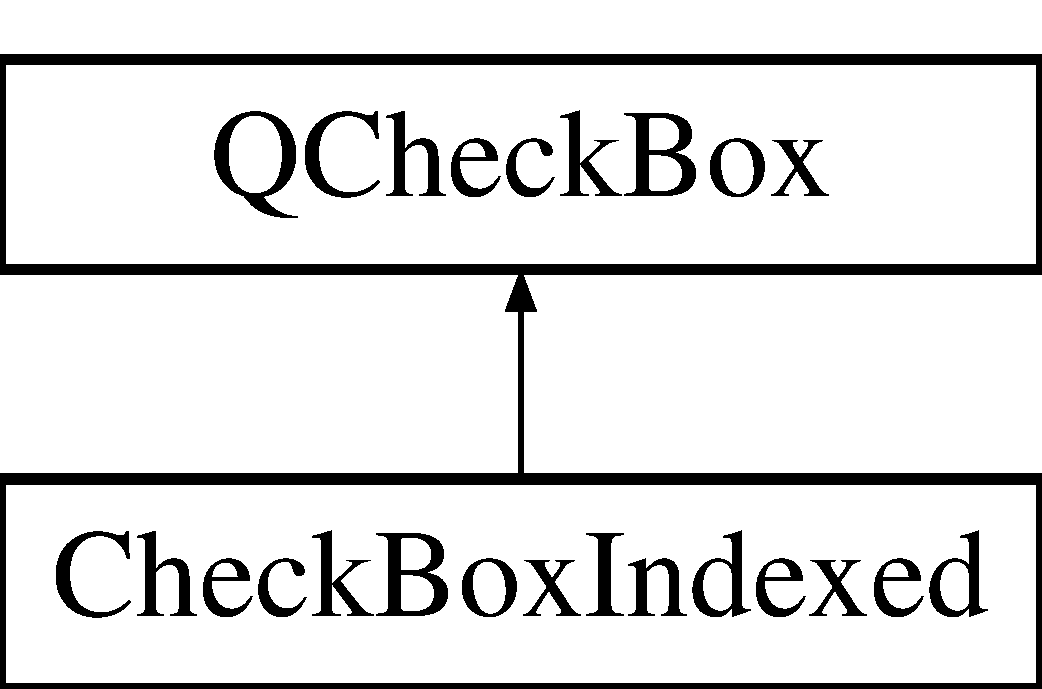
\includegraphics[height=2.000000cm]{classCheckBoxIndexed}
\end{center}
\end{figure}
\subsubsection*{Signals}
\begin{DoxyCompactItemize}
\item 
void \mbox{\hyperlink{classCheckBoxIndexed_a47301b2594e820c3ecf73c83e2ed0838}{clicked}} (int \mbox{\hyperlink{classCheckBoxIndexed_a044019936afecec6b18af69da0bf7c41}{index}})
\end{DoxyCompactItemize}
\subsubsection*{Public Member Functions}
\begin{DoxyCompactItemize}
\item 
\mbox{\hyperlink{classCheckBoxIndexed_a05d9d0ecbdfd394db281bdcfe256fb46}{Check\+Box\+Indexed}} (int \mbox{\hyperlink{classCheckBoxIndexed_a044019936afecec6b18af69da0bf7c41}{index}}, Q\+String text, Q\+Widget $\ast$parent=0)
\item 
virtual \mbox{\hyperlink{classCheckBoxIndexed_a2966a555ec25ced314dcc10b54ca6c54}{$\sim$\+Check\+Box\+Indexed}} ()
\end{DoxyCompactItemize}
\subsubsection*{Private Slots}
\begin{DoxyCompactItemize}
\item 
void \mbox{\hyperlink{classCheckBoxIndexed_a103f5e490ee87326b823c6ccab56d83c}{ch\+Clicked}} (bool)
\end{DoxyCompactItemize}
\subsubsection*{Private Attributes}
\begin{DoxyCompactItemize}
\item 
int \mbox{\hyperlink{classCheckBoxIndexed_a044019936afecec6b18af69da0bf7c41}{index}}
\end{DoxyCompactItemize}


\subsubsection{Constructor \& Destructor Documentation}
\mbox{\Hypertarget{classCheckBoxIndexed_a05d9d0ecbdfd394db281bdcfe256fb46}\label{classCheckBoxIndexed_a05d9d0ecbdfd394db281bdcfe256fb46}} 
\index{Check\+Box\+Indexed@{Check\+Box\+Indexed}!Check\+Box\+Indexed@{Check\+Box\+Indexed}}
\index{Check\+Box\+Indexed@{Check\+Box\+Indexed}!Check\+Box\+Indexed@{Check\+Box\+Indexed}}
\paragraph{\texorpdfstring{Check\+Box\+Indexed()}{CheckBoxIndexed()}}
{\footnotesize\ttfamily Check\+Box\+Indexed\+::\+Check\+Box\+Indexed (\begin{DoxyParamCaption}\item[{int}]{index,  }\item[{Q\+String}]{text,  }\item[{Q\+Widget $\ast$}]{parent = {\ttfamily 0} }\end{DoxyParamCaption})\hspace{0.3cm}{\ttfamily [inline]}}

\mbox{\Hypertarget{classCheckBoxIndexed_a2966a555ec25ced314dcc10b54ca6c54}\label{classCheckBoxIndexed_a2966a555ec25ced314dcc10b54ca6c54}} 
\index{Check\+Box\+Indexed@{Check\+Box\+Indexed}!````~Check\+Box\+Indexed@{$\sim$\+Check\+Box\+Indexed}}
\index{````~Check\+Box\+Indexed@{$\sim$\+Check\+Box\+Indexed}!Check\+Box\+Indexed@{Check\+Box\+Indexed}}
\paragraph{\texorpdfstring{$\sim$\+Check\+Box\+Indexed()}{~CheckBoxIndexed()}}
{\footnotesize\ttfamily virtual Check\+Box\+Indexed\+::$\sim$\+Check\+Box\+Indexed (\begin{DoxyParamCaption}{ }\end{DoxyParamCaption})\hspace{0.3cm}{\ttfamily [inline]}, {\ttfamily [virtual]}}



\subsubsection{Member Function Documentation}
\mbox{\Hypertarget{classCheckBoxIndexed_a103f5e490ee87326b823c6ccab56d83c}\label{classCheckBoxIndexed_a103f5e490ee87326b823c6ccab56d83c}} 
\index{Check\+Box\+Indexed@{Check\+Box\+Indexed}!ch\+Clicked@{ch\+Clicked}}
\index{ch\+Clicked@{ch\+Clicked}!Check\+Box\+Indexed@{Check\+Box\+Indexed}}
\paragraph{\texorpdfstring{ch\+Clicked}{chClicked}}
{\footnotesize\ttfamily void Check\+Box\+Indexed\+::ch\+Clicked (\begin{DoxyParamCaption}\item[{bool}]{ }\end{DoxyParamCaption})\hspace{0.3cm}{\ttfamily [inline]}, {\ttfamily [private]}, {\ttfamily [slot]}}

\mbox{\Hypertarget{classCheckBoxIndexed_a47301b2594e820c3ecf73c83e2ed0838}\label{classCheckBoxIndexed_a47301b2594e820c3ecf73c83e2ed0838}} 
\index{Check\+Box\+Indexed@{Check\+Box\+Indexed}!clicked@{clicked}}
\index{clicked@{clicked}!Check\+Box\+Indexed@{Check\+Box\+Indexed}}
\paragraph{\texorpdfstring{clicked}{clicked}}
{\footnotesize\ttfamily void Check\+Box\+Indexed\+::clicked (\begin{DoxyParamCaption}\item[{int}]{index }\end{DoxyParamCaption})\hspace{0.3cm}{\ttfamily [signal]}}



\subsubsection{Member Data Documentation}
\mbox{\Hypertarget{classCheckBoxIndexed_a044019936afecec6b18af69da0bf7c41}\label{classCheckBoxIndexed_a044019936afecec6b18af69da0bf7c41}} 
\index{Check\+Box\+Indexed@{Check\+Box\+Indexed}!index@{index}}
\index{index@{index}!Check\+Box\+Indexed@{Check\+Box\+Indexed}}
\paragraph{\texorpdfstring{index}{index}}
{\footnotesize\ttfamily int Check\+Box\+Indexed\+::index\hspace{0.3cm}{\ttfamily [private]}}



The documentation for this class was generated from the following file\+:\begin{DoxyCompactItemize}
\item 
\mbox{\hyperlink{headactivationdialog_8h}{headactivationdialog.\+h}}\end{DoxyCompactItemize}

\hypertarget{structComSettings}{}\subsection{Com\+Settings Struct Reference}
\label{structComSettings}\index{Com\+Settings@{Com\+Settings}}


{\ttfamily \#include $<$serialsettingsdialog.\+h$>$}

\subsubsection*{Public Member Functions}
\begin{DoxyCompactItemize}
\item 
\mbox{\hyperlink{structComSettings}{Com\+Settings}} \mbox{\hyperlink{structComSettings_ab648b02bb8d54eaa75afde8af0bb4218}{operator=}} (\mbox{\hyperlink{structComSettings}{Com\+Settings}} n\+Sett)
\end{DoxyCompactItemize}
\subsubsection*{Public Attributes}
Class of serial port setting. Class constructor have standard values of parameters to allow start program without setting file.
\begin{DoxyCompactItemize}
\item 
Q\+String \mbox{\hyperlink{structComSettings_aa21bef90f0730ae8f8f9f1ac612b4df0}{name}} = \char`\"{}/dev/tty\+S0\char`\"{}
\item 
qint32 \mbox{\hyperlink{structComSettings_ac34ef26d447e9053d85a3903f03f0f7e}{baud\+Rate}} = 38400
\item 
Q\+String \mbox{\hyperlink{structComSettings_a9d5a88e240b19b863c419d5cc05a4dec}{string\+Baud\+Rate}} = \char`\"{}38400\char`\"{}
\item 
Q\+Serial\+Port\+::\+Data\+Bits \mbox{\hyperlink{structComSettings_ac8eaec9f8e7a2951da30d16eff34c168}{data\+Bits}} = Q\+Serial\+Port\+::\+Data8
\item 
Q\+String \mbox{\hyperlink{structComSettings_a25ee68c643918b6c13f8e4e64a788c38}{string\+Data\+Bits}} = \char`\"{}8\char`\"{}
\item 
Q\+Serial\+Port\+::\+Parity \mbox{\hyperlink{structComSettings_a942d958bcaa7273d5b6589f92c922340}{parity}} = Q\+Serial\+Port\+::\+Odd\+Parity
\item 
Q\+String \mbox{\hyperlink{structComSettings_a21ad6c84428128867457f1e706500bcb}{string\+Parity}} = \char`\"{}Odd\char`\"{}
\item 
Q\+Serial\+Port\+::\+Stop\+Bits \mbox{\hyperlink{structComSettings_a3af1f4b81a956d46593badf8ea8a95ea}{stop\+Bits}} = Q\+Serial\+Port\+::\+One\+Stop
\item 
Q\+String \mbox{\hyperlink{structComSettings_a54ce036a24023acdd4b9f6460c7686c8}{string\+Stop\+Bits}} = \char`\"{}1\char`\"{}
\item 
Q\+Serial\+Port\+::\+Flow\+Control \mbox{\hyperlink{structComSettings_af719ceaf041eb31db53b2e5c189e0253}{flow\+Control}} = Q\+Serial\+Port\+::\+No\+Flow\+Control
\item 
Q\+String \mbox{\hyperlink{structComSettings_a23a3960bb4a476e74b49d1369352e7cc}{string\+Flow\+Control}} = \char`\"{}None\char`\"{}
\item 
bool \mbox{\hyperlink{structComSettings_ad276c73c919360c5bc5ff7996a2b6424}{local\+Echo\+Enabled}}
\end{DoxyCompactItemize}

\subsubsection{Member Function Documentation}
\index{Com\+Settings@{Com\+Settings}!operator=@{operator=}}
\index{operator=@{operator=}!Com\+Settings@{Com\+Settings}}
{\footnotesize\ttfamily \mbox{\hyperlink{structComSettings}{Com\+Settings}} Com\+Settings\+::\texorpdfstring{operator=()}{operator=()} (\begin{DoxyParamCaption}\item[{\mbox{\hyperlink{structComSettings}{Com\+Settings}}}]{n\+Sett }\end{DoxyParamCaption})} - Reimplemented standard operator. Allow copy parameters between two class object in simply way.

The documentation for this struct was generated from the following files\+:\begin{DoxyCompactItemize}
\item 
\mbox{\hyperlink{serialsettingsdialog_8h}{serialsettingsdialog.\+h}}\item 
\mbox{\hyperlink{serialsettingsdialog_8cpp}{serialsettingsdialog.\+cpp}}\end{DoxyCompactItemize}
\newpage
\hypertarget{classCountersDialog}{}\subsection{Counters\+Dialog Class Reference}
\label{classCountersDialog}\index{Counters\+Dialog@{Counters\+Dialog}}


{\ttfamily \#include $<$countersdialog.\+h$>$}

Inheritance diagram for Counters\+Dialog\+:\begin{figure}[H]
\begin{center}
\leavevmode
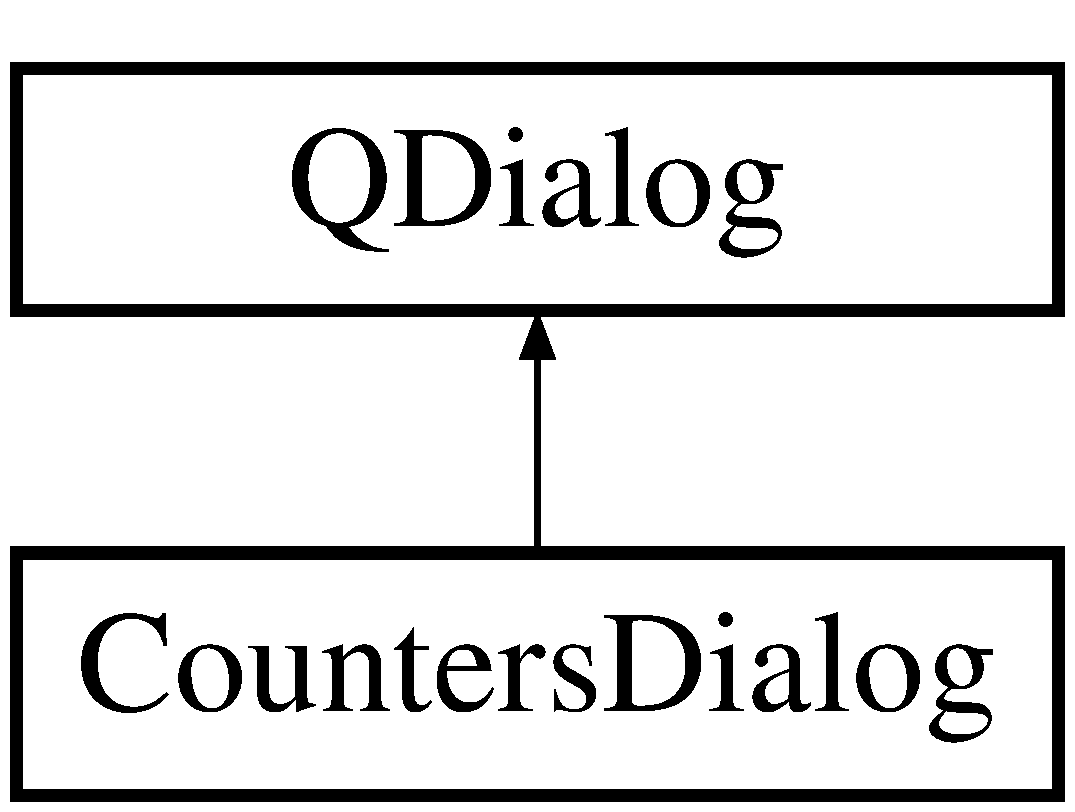
\includegraphics[height=2.000000cm]{classCountersDialog}
\end{center}
\end{figure}
\subsubsection*{Signals}
\begin{DoxyCompactItemize}
\item 
void \hyperlink{classCountersDialog_a721b63086592a577a17fada2c35fa8fa}{reset\+Skipped} ()
\item 
void \hyperlink{classCountersDialog_ad1642b578abe20a5a2bcb0ab8ecbd1cb}{reset\+Remaining} ()
\item 
void \hyperlink{classCountersDialog_a95672788db9b68ef07b0c251d6c1f0c8}{remaining\+Val\+Changed} (int val)
\end{DoxyCompactItemize}
\subsubsection*{Public Member Functions}
\begin{DoxyCompactItemize}
\item 
\hyperlink{classCountersDialog_a92f8263f1080effc36182051fdd06b72}{Counters\+Dialog} (Q\+Widget $\ast$parent=0)
\item 
\hyperlink{classCountersDialog_ab32b098f7b560b2fa550f51e0bba5863}{$\sim$\+Counters\+Dialog} ()
\item 
void \hyperlink{classCountersDialog_a40b2c28d1a33c2818ec9dea7063d0319}{set\+Remaining} (int val)
\end{DoxyCompactItemize}
\subsubsection*{Protected Member Functions}
\begin{DoxyCompactItemize}
\item 
bool \hyperlink{classCountersDialog_a4b3aca52961cf93da2b17a3266b27a12}{event} (Q\+Event $\ast$e)
\item 
void \hyperlink{classCountersDialog_af1e07b5f6ecf796c44a88cf3f58698e4}{show\+Event} (Q\+Show\+Event $\ast$ev)
\item 
bool \hyperlink{classCountersDialog_a93cf3132061916efd64757d22d4298a8}{event\+Filter} (Q\+Object $\ast$watched, Q\+Event $\ast$\hyperlink{classCountersDialog_a4b3aca52961cf93da2b17a3266b27a12}{event})
\item 
void \hyperlink{classCountersDialog_acc7e903ec5ff5b25631c7b1c810a123b}{change\+Event} (Q\+Event $\ast$\hyperlink{classCountersDialog_a4b3aca52961cf93da2b17a3266b27a12}{event})
\end{DoxyCompactItemize}
\subsubsection*{Private Slots}
\begin{DoxyCompactItemize}
\item 
void \hyperlink{classCountersDialog_a8e6ebaa6a437926644028d4fbf255a2d}{on\+\_\+push\+Button\+Remain\+Reset\+\_\+clicked} ()
\item 
void \hyperlink{classCountersDialog_aaa042f36e6a251055f135e67cfe711d6}{on\+\_\+push\+Button\+Skipped\+Reset\+\_\+clicked} ()
\item 
void \hyperlink{classCountersDialog_ac5e601c868667428b7cea2b53bfd674a}{on\+\_\+push\+Button\+Hide\+\_\+clicked} ()
\item 
void \hyperlink{classCountersDialog_ac3004e3c734190e156718361cf848394}{double\+Spin\+Box\+Remain\+\_\+value\+Changed} (double arg1)
\end{DoxyCompactItemize}
\subsubsection*{Private Attributes}
\begin{DoxyCompactItemize}
\item 
Ui\+::\+Counters\+Dialog $\ast$ \hyperlink{classCountersDialog_a6ca843a970b365e531602347eb2e231f}{ui}
\item 
bool \hyperlink{classCountersDialog_ad08acae2aa8655ed9956795b54f3b862}{accept\+On\+Deactilation\+En}
\end{DoxyCompactItemize}


\subsubsection{Constructor \& Destructor Documentation}
\index{Counters\+Dialog@{Counters\+Dialog}!Counters\+Dialog@{Counters\+Dialog}}
\index{Counters\+Dialog@{Counters\+Dialog}!Counters\+Dialog@{Counters\+Dialog}}
\paragraph[{\texorpdfstring{Counters\+Dialog(\+Q\+Widget $\ast$parent=0)}{CountersDialog(QWidget *parent=0)}}]{\setlength{\rightskip}{0pt plus 5cm}Counters\+Dialog\+::\+Counters\+Dialog (
\begin{DoxyParamCaption}
\item[{Q\+Widget $\ast$}]{parent = {\ttfamily 0}}
\end{DoxyParamCaption}
)\hspace{0.3cm}{\ttfamily [explicit]}}\hypertarget{classCountersDialog_a92f8263f1080effc36182051fdd06b72}{}\label{classCountersDialog_a92f8263f1080effc36182051fdd06b72}
\index{Counters\+Dialog@{Counters\+Dialog}!````~Counters\+Dialog@{$\sim$\+Counters\+Dialog}}
\index{````~Counters\+Dialog@{$\sim$\+Counters\+Dialog}!Counters\+Dialog@{Counters\+Dialog}}
\paragraph[{\texorpdfstring{$\sim$\+Counters\+Dialog()}{~CountersDialog()}}]{\setlength{\rightskip}{0pt plus 5cm}Counters\+Dialog\+::$\sim$\+Counters\+Dialog (
\begin{DoxyParamCaption}
{}
\end{DoxyParamCaption}
)}\hypertarget{classCountersDialog_ab32b098f7b560b2fa550f51e0bba5863}{}\label{classCountersDialog_ab32b098f7b560b2fa550f51e0bba5863}


\subsubsection{Member Function Documentation}
\index{Counters\+Dialog@{Counters\+Dialog}!change\+Event@{change\+Event}}
\index{change\+Event@{change\+Event}!Counters\+Dialog@{Counters\+Dialog}}
\paragraph[{\texorpdfstring{change\+Event(\+Q\+Event $\ast$event)}{changeEvent(QEvent *event)}}]{\setlength{\rightskip}{0pt plus 5cm}void Counters\+Dialog\+::change\+Event (
\begin{DoxyParamCaption}
\item[{Q\+Event $\ast$}]{event}
\end{DoxyParamCaption}
)\hspace{0.3cm}{\ttfamily [protected]}}\hypertarget{classCountersDialog_acc7e903ec5ff5b25631c7b1c810a123b}{}\label{classCountersDialog_acc7e903ec5ff5b25631c7b1c810a123b}
\index{Counters\+Dialog@{Counters\+Dialog}!double\+Spin\+Box\+Remain\+\_\+value\+Changed@{double\+Spin\+Box\+Remain\+\_\+value\+Changed}}
\index{double\+Spin\+Box\+Remain\+\_\+value\+Changed@{double\+Spin\+Box\+Remain\+\_\+value\+Changed}!Counters\+Dialog@{Counters\+Dialog}}
\paragraph[{\texorpdfstring{double\+Spin\+Box\+Remain\+\_\+value\+Changed}{doubleSpinBoxRemain_valueChanged}}]{\setlength{\rightskip}{0pt plus 5cm}void Counters\+Dialog\+::double\+Spin\+Box\+Remain\+\_\+value\+Changed (
\begin{DoxyParamCaption}
\item[{double}]{arg1}
\end{DoxyParamCaption}
)\hspace{0.3cm}{\ttfamily [private]}, {\ttfamily [slot]}}\hypertarget{classCountersDialog_ac3004e3c734190e156718361cf848394}{}\label{classCountersDialog_ac3004e3c734190e156718361cf848394}
\index{Counters\+Dialog@{Counters\+Dialog}!event@{event}}
\index{event@{event}!Counters\+Dialog@{Counters\+Dialog}}
\paragraph[{\texorpdfstring{event(\+Q\+Event $\ast$e)}{event(QEvent *e)}}]{\setlength{\rightskip}{0pt plus 5cm}bool Counters\+Dialog\+::event (
\begin{DoxyParamCaption}
\item[{Q\+Event $\ast$}]{e}
\end{DoxyParamCaption}
)\hspace{0.3cm}{\ttfamily [protected]}}\hypertarget{classCountersDialog_a4b3aca52961cf93da2b17a3266b27a12}{}\label{classCountersDialog_a4b3aca52961cf93da2b17a3266b27a12}
\index{Counters\+Dialog@{Counters\+Dialog}!event\+Filter@{event\+Filter}}
\index{event\+Filter@{event\+Filter}!Counters\+Dialog@{Counters\+Dialog}}
\paragraph[{\texorpdfstring{event\+Filter(\+Q\+Object $\ast$watched, Q\+Event $\ast$event)}{eventFilter(QObject *watched, QEvent *event)}}]{\setlength{\rightskip}{0pt plus 5cm}bool Counters\+Dialog\+::event\+Filter (
\begin{DoxyParamCaption}
\item[{Q\+Object $\ast$}]{watched, }
\item[{Q\+Event $\ast$}]{event}
\end{DoxyParamCaption}
)\hspace{0.3cm}{\ttfamily [protected]}}\hypertarget{classCountersDialog_a93cf3132061916efd64757d22d4298a8}{}\label{classCountersDialog_a93cf3132061916efd64757d22d4298a8}
\index{Counters\+Dialog@{Counters\+Dialog}!on\+\_\+push\+Button\+Hide\+\_\+clicked@{on\+\_\+push\+Button\+Hide\+\_\+clicked}}
\index{on\+\_\+push\+Button\+Hide\+\_\+clicked@{on\+\_\+push\+Button\+Hide\+\_\+clicked}!Counters\+Dialog@{Counters\+Dialog}}
\paragraph[{\texorpdfstring{on\+\_\+push\+Button\+Hide\+\_\+clicked}{on_pushButtonHide_clicked}}]{\setlength{\rightskip}{0pt plus 5cm}void Counters\+Dialog\+::on\+\_\+push\+Button\+Hide\+\_\+clicked (
\begin{DoxyParamCaption}
{}
\end{DoxyParamCaption}
)\hspace{0.3cm}{\ttfamily [private]}, {\ttfamily [slot]}}\hypertarget{classCountersDialog_ac5e601c868667428b7cea2b53bfd674a}{}\label{classCountersDialog_ac5e601c868667428b7cea2b53bfd674a}
\index{Counters\+Dialog@{Counters\+Dialog}!on\+\_\+push\+Button\+Remain\+Reset\+\_\+clicked@{on\+\_\+push\+Button\+Remain\+Reset\+\_\+clicked}}
\index{on\+\_\+push\+Button\+Remain\+Reset\+\_\+clicked@{on\+\_\+push\+Button\+Remain\+Reset\+\_\+clicked}!Counters\+Dialog@{Counters\+Dialog}}
\paragraph[{\texorpdfstring{on\+\_\+push\+Button\+Remain\+Reset\+\_\+clicked}{on_pushButtonRemainReset_clicked}}]{\setlength{\rightskip}{0pt plus 5cm}void Counters\+Dialog\+::on\+\_\+push\+Button\+Remain\+Reset\+\_\+clicked (
\begin{DoxyParamCaption}
{}
\end{DoxyParamCaption}
)\hspace{0.3cm}{\ttfamily [private]}, {\ttfamily [slot]}}\hypertarget{classCountersDialog_a8e6ebaa6a437926644028d4fbf255a2d}{}\label{classCountersDialog_a8e6ebaa6a437926644028d4fbf255a2d}
\index{Counters\+Dialog@{Counters\+Dialog}!on\+\_\+push\+Button\+Skipped\+Reset\+\_\+clicked@{on\+\_\+push\+Button\+Skipped\+Reset\+\_\+clicked}}
\index{on\+\_\+push\+Button\+Skipped\+Reset\+\_\+clicked@{on\+\_\+push\+Button\+Skipped\+Reset\+\_\+clicked}!Counters\+Dialog@{Counters\+Dialog}}
\paragraph[{\texorpdfstring{on\+\_\+push\+Button\+Skipped\+Reset\+\_\+clicked}{on_pushButtonSkippedReset_clicked}}]{\setlength{\rightskip}{0pt plus 5cm}void Counters\+Dialog\+::on\+\_\+push\+Button\+Skipped\+Reset\+\_\+clicked (
\begin{DoxyParamCaption}
{}
\end{DoxyParamCaption}
)\hspace{0.3cm}{\ttfamily [private]}, {\ttfamily [slot]}}\hypertarget{classCountersDialog_aaa042f36e6a251055f135e67cfe711d6}{}\label{classCountersDialog_aaa042f36e6a251055f135e67cfe711d6}
\index{Counters\+Dialog@{Counters\+Dialog}!remaining\+Val\+Changed@{remaining\+Val\+Changed}}
\index{remaining\+Val\+Changed@{remaining\+Val\+Changed}!Counters\+Dialog@{Counters\+Dialog}}
\paragraph[{\texorpdfstring{remaining\+Val\+Changed}{remainingValChanged}}]{\setlength{\rightskip}{0pt plus 5cm}void Counters\+Dialog\+::remaining\+Val\+Changed (
\begin{DoxyParamCaption}
\item[{int}]{val}
\end{DoxyParamCaption}
)\hspace{0.3cm}{\ttfamily [signal]}}\hypertarget{classCountersDialog_a95672788db9b68ef07b0c251d6c1f0c8}{}\label{classCountersDialog_a95672788db9b68ef07b0c251d6c1f0c8}
\index{Counters\+Dialog@{Counters\+Dialog}!reset\+Remaining@{reset\+Remaining}}
\index{reset\+Remaining@{reset\+Remaining}!Counters\+Dialog@{Counters\+Dialog}}
\paragraph[{\texorpdfstring{reset\+Remaining}{resetRemaining}}]{\setlength{\rightskip}{0pt plus 5cm}void Counters\+Dialog\+::reset\+Remaining (
\begin{DoxyParamCaption}
{}
\end{DoxyParamCaption}
)\hspace{0.3cm}{\ttfamily [signal]}}\hypertarget{classCountersDialog_ad1642b578abe20a5a2bcb0ab8ecbd1cb}{}\label{classCountersDialog_ad1642b578abe20a5a2bcb0ab8ecbd1cb}
\index{Counters\+Dialog@{Counters\+Dialog}!reset\+Skipped@{reset\+Skipped}}
\index{reset\+Skipped@{reset\+Skipped}!Counters\+Dialog@{Counters\+Dialog}}
\paragraph[{\texorpdfstring{reset\+Skipped}{resetSkipped}}]{\setlength{\rightskip}{0pt plus 5cm}void Counters\+Dialog\+::reset\+Skipped (
\begin{DoxyParamCaption}
{}
\end{DoxyParamCaption}
)\hspace{0.3cm}{\ttfamily [signal]}}\hypertarget{classCountersDialog_a721b63086592a577a17fada2c35fa8fa}{}\label{classCountersDialog_a721b63086592a577a17fada2c35fa8fa}
\index{Counters\+Dialog@{Counters\+Dialog}!set\+Remaining@{set\+Remaining}}
\index{set\+Remaining@{set\+Remaining}!Counters\+Dialog@{Counters\+Dialog}}
\paragraph[{\texorpdfstring{set\+Remaining(int val)}{setRemaining(int val)}}]{\setlength{\rightskip}{0pt plus 5cm}void Counters\+Dialog\+::set\+Remaining (
\begin{DoxyParamCaption}
\item[{int}]{val}
\end{DoxyParamCaption}
)}\hypertarget{classCountersDialog_a40b2c28d1a33c2818ec9dea7063d0319}{}\label{classCountersDialog_a40b2c28d1a33c2818ec9dea7063d0319}
\index{Counters\+Dialog@{Counters\+Dialog}!show\+Event@{show\+Event}}
\index{show\+Event@{show\+Event}!Counters\+Dialog@{Counters\+Dialog}}
\paragraph[{\texorpdfstring{show\+Event(\+Q\+Show\+Event $\ast$ev)}{showEvent(QShowEvent *ev)}}]{\setlength{\rightskip}{0pt plus 5cm}void Counters\+Dialog\+::show\+Event (
\begin{DoxyParamCaption}
\item[{Q\+Show\+Event $\ast$}]{ev}
\end{DoxyParamCaption}
)\hspace{0.3cm}{\ttfamily [protected]}}\hypertarget{classCountersDialog_af1e07b5f6ecf796c44a88cf3f58698e4}{}\label{classCountersDialog_af1e07b5f6ecf796c44a88cf3f58698e4}


\subsubsection{Member Data Documentation}
\index{Counters\+Dialog@{Counters\+Dialog}!accept\+On\+Deactilation\+En@{accept\+On\+Deactilation\+En}}
\index{accept\+On\+Deactilation\+En@{accept\+On\+Deactilation\+En}!Counters\+Dialog@{Counters\+Dialog}}
\paragraph[{\texorpdfstring{accept\+On\+Deactilation\+En}{acceptOnDeactilationEn}}]{\setlength{\rightskip}{0pt plus 5cm}bool Counters\+Dialog\+::accept\+On\+Deactilation\+En\hspace{0.3cm}{\ttfamily [private]}}\hypertarget{classCountersDialog_ad08acae2aa8655ed9956795b54f3b862}{}\label{classCountersDialog_ad08acae2aa8655ed9956795b54f3b862}
\index{Counters\+Dialog@{Counters\+Dialog}!ui@{ui}}
\index{ui@{ui}!Counters\+Dialog@{Counters\+Dialog}}
\paragraph[{\texorpdfstring{ui}{ui}}]{\setlength{\rightskip}{0pt plus 5cm}Ui\+::\+Counters\+Dialog$\ast$ Counters\+Dialog\+::ui\hspace{0.3cm}{\ttfamily [private]}}\hypertarget{classCountersDialog_a6ca843a970b365e531602347eb2e231f}{}\label{classCountersDialog_a6ca843a970b365e531602347eb2e231f}


The documentation for this class was generated from the following files\+:\begin{DoxyCompactItemize}
\item 
\hyperlink{countersdialog_8h}{countersdialog.\+h}\item 
\hyperlink{countersdialog_8cpp}{countersdialog.\+cpp}\end{DoxyCompactItemize}

\hypertarget{classCrcCalc}{}\subsection{Crc\+Calc Class Reference}
\label{classCrcCalc}\index{Crc\+Calc@{Crc\+Calc}}
{\ttfamily \#include $<$crc16.\+h$>$}\\
Class contain two static function to calculate CRC16 value in two way: with or without CRC table.\\
Functions are used without creating class object and are inline to optimize program.

\subsubsection*{Public Member Functions}
\begin{DoxyCompactItemize}
\item 
\mbox{\hyperlink{classCrcCalc_a9e3d8fbe834f69aeb8a21a16e26bfa1f}{Crc\+Calc}} ()
\end{DoxyCompactItemize}
\subsubsection*{Static Public Member Functions}
\begin{DoxyCompactItemize}
\item 
static \mbox{\hyperlink{settings_8h_a017dd44e68049ffdd31500a8cd01ba68}{uint16\+\_\+t}} \mbox{\hyperlink{classCrcCalc_af903157f70d448ef1dd660f8580ba0c6}{Calculate\+C\+R\+C16}} (\mbox{\hyperlink{settings_8h_a017dd44e68049ffdd31500a8cd01ba68}{uint16\+\_\+t}} crc, Q\+Byte\+Array c\+\_\+ptr)
\item 
static \mbox{\hyperlink{settings_8h_a017dd44e68049ffdd31500a8cd01ba68}{uint16\+\_\+t}} \mbox{\hyperlink{classCrcCalc_aa4d7542b130a13fb3d675b885cfadbbd}{Calculate\+C\+R\+C16}} (Q\+Byte\+Array inp\+Arr)
\end{DoxyCompactItemize}

\subsubsection{Member Function Documentation}
\mbox{\Hypertarget{classCrcCalc_af903157f70d448ef1dd660f8580ba0c6}\label{classCrcCalc_af903157f70d448ef1dd660f8580ba0c6}} 
\index{Crc\+Calc@{Crc\+Calc}!Calculate\+C\+R\+C16@{Calculate\+C\+R\+C16}}
\index{Calculate\+C\+R\+C16@{Calculate\+C\+R\+C16}!Crc\+Calc@{Crc\+Calc}}
\paragraph{\texorpdfstring{Calculate\+C\+R\+C16()}{CalculateCRC16()}{\footnotesize\ttfamily [1/2]}}
Calculate CRC without table. Used for communication between PC and machine master board.\\
{\footnotesize\ttfamily static \mbox{\hyperlink{settings_8h_a017dd44e68049ffdd31500a8cd01ba68}{uint16\+\_\+t}} Crc\+Calc\+::\+Calculate\+C\+R\+C16 (\begin{DoxyParamCaption}\item[{\mbox{\hyperlink{settings_8h_a017dd44e68049ffdd31500a8cd01ba68}{uint16\+\_\+t}}}]{crc,  }\item[{Q\+Byte\+Array}]{c\+\_\+ptr }\end{DoxyParamCaption}){\ttfamily [inline]}, {\ttfamily [static]}}

\mbox{\Hypertarget{classCrcCalc_aa4d7542b130a13fb3d675b885cfadbbd}\label{classCrcCalc_aa4d7542b130a13fb3d675b885cfadbbd}} 
\index{Crc\+Calc@{Crc\+Calc}!Calculate\+C\+R\+C16@{Calculate\+C\+R\+C16}}
\index{Calculate\+C\+R\+C16@{Calculate\+C\+R\+C16}!Crc\+Calc@{Crc\+Calc}}
\paragraph{\texorpdfstring{Calculate\+C\+R\+C16()}{CalculateCRC16()}{\footnotesize\ttfamily [2/2]}}
Calculate CRC with written table. Can be used to communicate with HMI or other similar devices.\\
{\footnotesize\ttfamily static \mbox{\hyperlink{settings_8h_a017dd44e68049ffdd31500a8cd01ba68}{uint16\+\_\+t}} Crc\+Calc\+::\+Calculate\+C\+R\+C16 (\begin{DoxyParamCaption}\item[{Q\+Byte\+Array}]{inp\+Arr }\end{DoxyParamCaption})\hspace{0.3cm}{\ttfamily [inline]}, {\ttfamily [static]}}

The documentation for this class was generated from the following file\+:\begin{DoxyCompactItemize}
\item 
\mbox{\hyperlink{crc16_8h}{crc16.\+h}}\end{DoxyCompactItemize}
\newpage
\hypertarget{classCyclesDialog}{}\subsection{Cycles\+Dialog Class Reference}
\label{classCyclesDialog}\index{Cycles\+Dialog@{Cycles\+Dialog}}
{\ttfamily \#include $<$cyclesdialog.\+h$>$}

Inheritance diagram for Cycles\+Dialog\+:\begin{figure}[H]
\begin{center}
\leavevmode
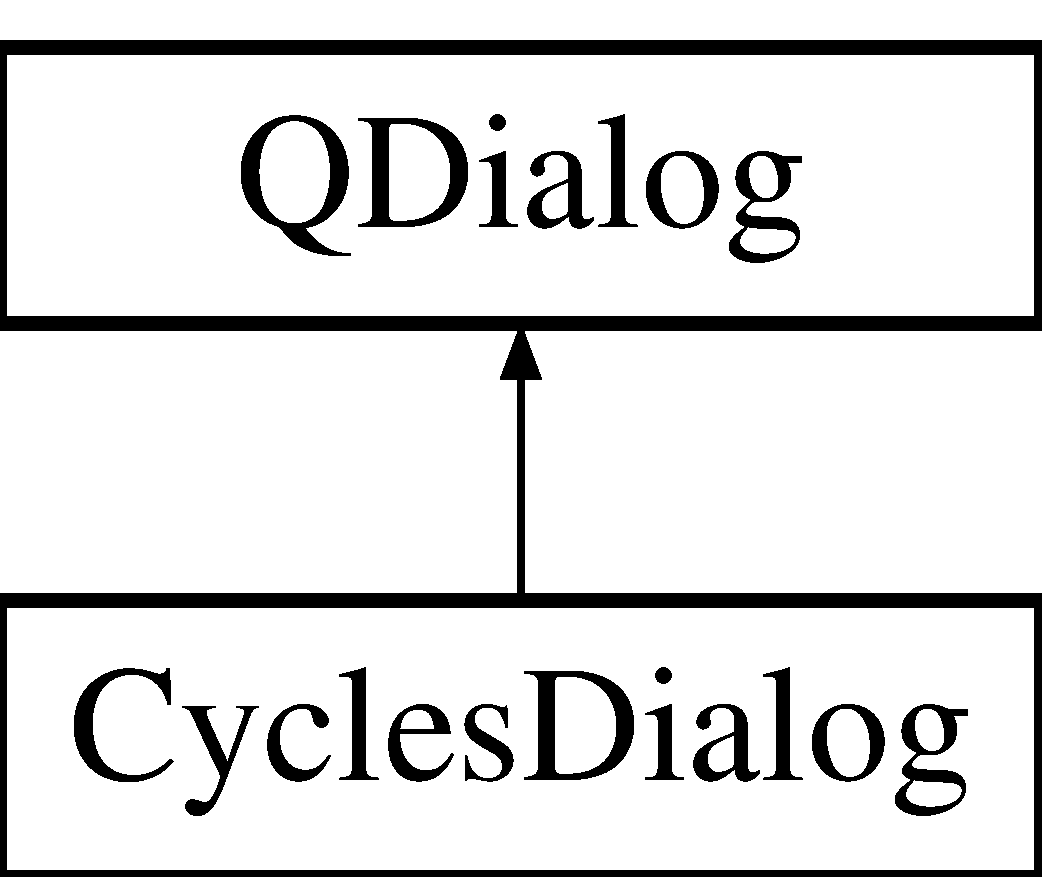
\includegraphics[height=2.000000cm]{classCyclesDialog}
\end{center}
\end{figure}
\subsubsection*{Signals}
\begin{DoxyCompactItemize}
\item 
void \mbox{\hyperlink{classCyclesDialog_a6dabe9aeecfb9264a4b6014d74241432}{send\+Command}} (Q\+Byte\+Array cnd\+Arr)
\end{DoxyCompactItemize}
\subsubsection*{Public Member Functions}
\begin{DoxyCompactItemize}
\item 
\mbox{\hyperlink{classCyclesDialog_a0fa891942095d90fef41ec6aa8fa3860}{Cycles\+Dialog}} (Q\+Widget $\ast$parent=0)
\item 
\mbox{\hyperlink{classCyclesDialog_a3eeb8a5c3baba2d43c604981cb3eceaa}{Cycles\+Dialog}} (int \mbox{\hyperlink{classCyclesDialog_aaa0b334934a65c2bf2ef231a31199779}{head\+Count}}, Q\+Widget $\ast$parent=0)
\item 
\mbox{\hyperlink{classCyclesDialog_ad4da02e07b34c1d7e4aaad3bffab2246}{$\sim$\+Cycles\+Dialog}} ()
\end{DoxyCompactItemize}
\subsubsection*{Protected Member Functions}
\begin{DoxyCompactItemize}
\item 
void \mbox{\hyperlink{classCyclesDialog_a43494fe7c65472212974a7be28a31d3d}{show\+Event}} (Q\+Show\+Event $\ast$ev)
\item 
bool \mbox{\hyperlink{classCyclesDialog_a5a20052e29f7530886dded1e06bc5afd}{event\+Filter}} (Q\+Object $\ast$watched, Q\+Event $\ast$event)
\item 
void \mbox{\hyperlink{classCyclesDialog_a3d1b7bb4af1e286adadf2483cb0e4dfe}{change\+Event}} (Q\+Event $\ast$event)
\end{DoxyCompactItemize}
\subsubsection*{Private Slots}
\begin{DoxyCompactItemize}
\item 
void \mbox{\hyperlink{classCyclesDialog_a5e6a1c6ccd9ad82de8f0ecdc8b3e064a}{on\+\_\+p\+Button\+O\+K\+\_\+clicked}} ()
\item 
void \mbox{\hyperlink{classCyclesDialog_a6f7d5b5e90af9ba725ac2432f5490d92}{on\+\_\+p\+Button\+O\+N\+\_\+clicked}} ()
\item 
void \mbox{\hyperlink{classCyclesDialog_a1e4ad2ee11ec162987d24e2071c3f5c4}{on\+\_\+p\+Button\+Prev\+\_\+clicked}} ()
\item 
void \mbox{\hyperlink{classCyclesDialog_a2f918e498a7c5cd77b12edb6923fb78d}{on\+\_\+p\+Button\+Next\+\_\+clicked}} ()
\item 
void \mbox{\hyperlink{classCyclesDialog_a0ce26519321c0a05a2829861468575b8}{on\+\_\+p\+Button\+C1\+\_\+clicked}} ()
\item 
void \mbox{\hyperlink{classCyclesDialog_ab71f6eda48eafb78e6c57ad91855b2ae}{on\+\_\+p\+Button\+C2\+\_\+clicked}} ()
\item 
void \mbox{\hyperlink{classCyclesDialog_a85b601531f06911a6e3ebacafdfd44cf}{on\+\_\+p\+Button\+C3\+\_\+clicked}} ()
\item 
void \mbox{\hyperlink{classCyclesDialog_a46d7c69940f9359064611b836c39e09c}{on\+\_\+p\+Button\+C4\+\_\+clicked}} ()
\item 
void \mbox{\hyperlink{classCyclesDialog_ab25cdb8d2757b90a2a041e132a8f62fe}{on\+\_\+p\+Button\+C5\+\_\+clicked}} ()
\item 
void \mbox{\hyperlink{classCyclesDialog_a261ffb4571e95cc74ad443d38edf4194}{on\+\_\+p\+Button\+C6\+\_\+clicked}} ()
\item 
void \mbox{\hyperlink{classCyclesDialog_a84f771b37567f71fc3012dbcd2bd56e5}{on\+\_\+p\+Button\+C7\+\_\+clicked}} ()
\item 
void \mbox{\hyperlink{classCyclesDialog_aca041160847e154ae7ad73a8dc90501d}{on\+\_\+p\+Button\+C8\+\_\+clicked}} ()
\item 
void \mbox{\hyperlink{classCyclesDialog_ad25bef71c8a2219252c1458fa333a376}{load\+Values}} (int $\ast$vals)
\item 
void \mbox{\hyperlink{classCyclesDialog_a26c86ed543a9345f230fb8925ccae5d9}{save\+Values}} (void)
\end{DoxyCompactItemize}
\subsubsection*{Private Attributes}
\begin{DoxyCompactItemize}
\item 
Ui\+::\+Cycles\+Dialog $\ast$ \mbox{\hyperlink{classCyclesDialog_a40d0b1d840144ae10ec8269fafc77ea1}{ui}}
\item 
int \mbox{\hyperlink{classCyclesDialog_aaa0b334934a65c2bf2ef231a31199779}{head\+Count}}
\item 
Q\+List$<$ Q\+Double\+Spin\+Box $\ast$ $>$ \mbox{\hyperlink{classCyclesDialog_a322448cc7948ab1d5fce41291fbfab5a}{spin\+Box\+List}}
\item 
Q\+List$<$ Q\+Label $\ast$ $>$ \mbox{\hyperlink{classCyclesDialog_a3c6c74691e32ce18a38b8002917b6734}{label\+List}}
\item 
int \mbox{\hyperlink{classCyclesDialog_a1b608c6d6ebf52a902645ee910f91ffa}{last\+Cycle\+Sel}}
\item 
Q\+List$<$ int $\ast$ $>$ \mbox{\hyperlink{classCyclesDialog_a6c5035971ebd473201fa9c62e58fee3a}{cycle\+Values}}
\item 
int \mbox{\hyperlink{classCyclesDialog_a0296f0dc0b57b44f6d69e1a9b5cc00ad}{cycle\+State}}
\item 
Q\+Settings $\ast$ \mbox{\hyperlink{classCyclesDialog_aaf91e761bb72e2603988719a671aab3b}{cycle\+Settings}}
\item 
Q\+List$<$ \mbox{\hyperlink{settings_8h_a4196118492a3b1493c81f250e90af775}{uint32\+\_\+t}} $>$ \mbox{\hyperlink{classCyclesDialog_aa847f1b8721dff01575a9600da120a3a}{head\+State\+List}}
\item 
Q\+List$<$ \mbox{\hyperlink{settings_8h_a4196118492a3b1493c81f250e90af775}{uint32\+\_\+t}} $>$ \mbox{\hyperlink{classCyclesDialog_a1f87902a8d3b08aadc86fe1ef83ccca9}{head\+Strok\+List}}
\end{DoxyCompactItemize}


\subsubsection{Constructor \& Destructor Documentation}
\mbox{\Hypertarget{classCyclesDialog_a0fa891942095d90fef41ec6aa8fa3860}\label{classCyclesDialog_a0fa891942095d90fef41ec6aa8fa3860}} 
\index{Cycles\+Dialog@{Cycles\+Dialog}!Cycles\+Dialog@{Cycles\+Dialog}}
\index{Cycles\+Dialog@{Cycles\+Dialog}!Cycles\+Dialog@{Cycles\+Dialog}}
\paragraph{\texorpdfstring{Cycles\+Dialog()}{CyclesDialog()}{\footnotesize\ttfamily [1/2]}}
Empty constructor (default). Not used in project.\\
{\footnotesize\ttfamily Cycles\+Dialog\+::\+Cycles\+Dialog (\begin{DoxyParamCaption}\item[{Q\+Widget $\ast$}]{parent = {\ttfamily 0} }\end{DoxyParamCaption}){\ttfamily [explicit]}}
\mbox{\Hypertarget{classCyclesDialog_a3eeb8a5c3baba2d43c604981cb3eceaa}\label{classCyclesDialog_a3eeb8a5c3baba2d43c604981cb3eceaa}} 
\index{Cycles\+Dialog@{Cycles\+Dialog}!Cycles\+Dialog@{Cycles\+Dialog}}
\index{Cycles\+Dialog@{Cycles\+Dialog}!Cycles\+Dialog@{Cycles\+Dialog}}
\paragraph{\texorpdfstring{Cycles\+Dialog()}{CyclesDialog()}{\footnotesize\ttfamily [2/2]}}
Class constructor. Sets count of heads of machine to create and layout widget of dialog.\\
{\footnotesize\ttfamily Cycles\+Dialog\+::\+Cycles\+Dialog (\begin{DoxyParamCaption}\item[{int}]{head\+Count,  }\item[{Q\+Widget $\ast$}]{parent = {\ttfamily 0} }\end{DoxyParamCaption}){\ttfamily [explicit]}}

\mbox{\Hypertarget{classCyclesDialog_ad4da02e07b34c1d7e4aaad3bffab2246}\label{classCyclesDialog_ad4da02e07b34c1d7e4aaad3bffab2246}} 
\index{Cycles\+Dialog@{Cycles\+Dialog}!````~Cycles\+Dialog@{$\sim$\+Cycles\+Dialog}}
\index{````~Cycles\+Dialog@{$\sim$\+Cycles\+Dialog}!Cycles\+Dialog@{Cycles\+Dialog}}
\paragraph{\texorpdfstring{$\sim$\+Cycles\+Dialog()}{~CyclesDialog()}}
{\footnotesize\ttfamily Cycles\+Dialog\+::$\sim$\+Cycles\+Dialog (\begin{DoxyParamCaption}{ }\end{DoxyParamCaption})}

\subsubsection{Member Function Documentation}
\mbox{\Hypertarget{classCyclesDialog_a3d1b7bb4af1e286adadf2483cb0e4dfe}\label{classCyclesDialog_a3d1b7bb4af1e286adadf2483cb0e4dfe}} 
\index{Cycles\+Dialog@{Cycles\+Dialog}!change\+Event@{change\+Event}}
\index{change\+Event@{change\+Event}!Cycles\+Dialog@{Cycles\+Dialog}}
{\footnotesize\ttfamily void Cycles\+Dialog\+::\texorpdfstring{change\+Event()}{changeEvent()} (\begin{DoxyParamCaption}\item[{Q\+Event $\ast$}]{event }\end{DoxyParamCaption}){\ttfamily [protected]}} - reimplementation of default event for QDialog to enable user interface translation. Function called automatically.

\mbox{\Hypertarget{classCyclesDialog_a5a20052e29f7530886dded1e06bc5afd}\label{classCyclesDialog_a5a20052e29f7530886dded1e06bc5afd}} 
\index{Cycles\+Dialog@{Cycles\+Dialog}!event\+Filter@{event\+Filter}}
\index{event\+Filter@{event\+Filter}!Cycles\+Dialog@{Cycles\+Dialog}}
\paragraph{\texorpdfstring{event\+Filter()}{eventFilter()}}
Mouse event filter to call on-screen numeric key to enter values to appropriate QSpinBoxes. Function called automatically.\\
{\footnotesize\ttfamily bool Cycles\+Dialog\+::event\+Filter (\begin{DoxyParamCaption}\item[{Q\+Object $\ast$}]{watched,  }\item[{Q\+Event $\ast$}]{event }\end{DoxyParamCaption}){\ttfamily [protected]}}

\mbox{\Hypertarget{classCyclesDialog_ad25bef71c8a2219252c1458fa333a376}\label{classCyclesDialog_ad25bef71c8a2219252c1458fa333a376}} 
\index{Cycles\+Dialog@{Cycles\+Dialog}!load\+Values@{load\+Values}}
\index{load\+Values@{load\+Values}!Cycles\+Dialog@{Cycles\+Dialog}}
\paragraph{\texorpdfstring{load\+Values}{loadValues}}
Function load values to appropriate QSpinBoxes form Q\+List$<$int$\ast$ $>$ \mbox{\hyperlink{classCyclesDialog_a6c5035971ebd473201fa9c62e58fee3a}{cycle\+Values}} list with consideration of selected cycle by variable \mbox{\hyperlink{classCyclesDialog_a1b608c6d6ebf52a902645ee910f91ffa}{last\+Cycle\+Sel}}.\\
{\footnotesize\ttfamily void Cycles\+Dialog\+::load\+Values (\begin{DoxyParamCaption}\item[{int $\ast$}]{vals }\end{DoxyParamCaption}){\ttfamily [private]}, {\ttfamily [slot]}}
\mbox{\Hypertarget{classCyclesDialog_a0ce26519321c0a05a2829861468575b8}\label{classCyclesDialog_a0ce26519321c0a05a2829861468575b8}} 
\index{Cycles\+Dialog@{Cycles\+Dialog}!on\+\_\+p\+Button\+C1\+\_\+clicked@{on\+\_\+p\+Button\+C1\+\_\+clicked}}
\index{on\+\_\+p\+Button\+C1\+\_\+clicked@{on\+\_\+p\+Button\+C1\+\_\+clicked}!Cycles\+Dialog@{Cycles\+Dialog}}
\mbox{\Hypertarget{classCyclesDialog_ab71f6eda48eafb78e6c57ad91855b2ae}\label{classCyclesDialog_ab71f6eda48eafb78e6c57ad91855b2ae}} 
\index{Cycles\+Dialog@{Cycles\+Dialog}!on\+\_\+p\+Button\+C2\+\_\+clicked@{on\+\_\+p\+Button\+C2\+\_\+clicked}}
\index{on\+\_\+p\+Button\+C2\+\_\+clicked@{on\+\_\+p\+Button\+C2\+\_\+clicked}!Cycles\+Dialog@{Cycles\+Dialog}}
\mbox{\Hypertarget{classCyclesDialog_a85b601531f06911a6e3ebacafdfd44cf}\label{classCyclesDialog_a85b601531f06911a6e3ebacafdfd44cf}} 
\index{Cycles\+Dialog@{Cycles\+Dialog}!on\+\_\+p\+Button\+C3\+\_\+clicked@{on\+\_\+p\+Button\+C3\+\_\+clicked}}
\index{on\+\_\+p\+Button\+C3\+\_\+clicked@{on\+\_\+p\+Button\+C3\+\_\+clicked}!Cycles\+Dialog@{Cycles\+Dialog}}
\mbox{\Hypertarget{classCyclesDialog_a46d7c69940f9359064611b836c39e09c}\label{classCyclesDialog_a46d7c69940f9359064611b836c39e09c}} 
\index{Cycles\+Dialog@{Cycles\+Dialog}!on\+\_\+p\+Button\+C4\+\_\+clicked@{on\+\_\+p\+Button\+C4\+\_\+clicked}}
\index{on\+\_\+p\+Button\+C4\+\_\+clicked@{on\+\_\+p\+Button\+C4\+\_\+clicked}!Cycles\+Dialog@{Cycles\+Dialog}}
\mbox{\Hypertarget{classCyclesDialog_ab25cdb8d2757b90a2a041e132a8f62fe}\label{classCyclesDialog_ab25cdb8d2757b90a2a041e132a8f62fe}} 
\index{Cycles\+Dialog@{Cycles\+Dialog}!on\+\_\+p\+Button\+C5\+\_\+clicked@{on\+\_\+p\+Button\+C5\+\_\+clicked}}
\index{on\+\_\+p\+Button\+C5\+\_\+clicked@{on\+\_\+p\+Button\+C5\+\_\+clicked}!Cycles\+Dialog@{Cycles\+Dialog}}
\mbox{\Hypertarget{classCyclesDialog_a261ffb4571e95cc74ad443d38edf4194}\label{classCyclesDialog_a261ffb4571e95cc74ad443d38edf4194}} 
\index{Cycles\+Dialog@{Cycles\+Dialog}!on\+\_\+p\+Button\+C6\+\_\+clicked@{on\+\_\+p\+Button\+C6\+\_\+clicked}}
\index{on\+\_\+p\+Button\+C6\+\_\+clicked@{on\+\_\+p\+Button\+C6\+\_\+clicked}!Cycles\+Dialog@{Cycles\+Dialog}}
\mbox{\Hypertarget{classCyclesDialog_a84f771b37567f71fc3012dbcd2bd56e5}\label{classCyclesDialog_a84f771b37567f71fc3012dbcd2bd56e5}} 
\index{Cycles\+Dialog@{Cycles\+Dialog}!on\+\_\+p\+Button\+C7\+\_\+clicked@{on\+\_\+p\+Button\+C7\+\_\+clicked}}
\index{on\+\_\+p\+Button\+C7\+\_\+clicked@{on\+\_\+p\+Button\+C7\+\_\+clicked}!Cycles\+Dialog@{Cycles\+Dialog}}
\mbox{\Hypertarget{classCyclesDialog_aca041160847e154ae7ad73a8dc90501d}\label{classCyclesDialog_aca041160847e154ae7ad73a8dc90501d}} 
\index{Cycles\+Dialog@{Cycles\+Dialog}!on\+\_\+p\+Button\+C8\+\_\+clicked@{on\+\_\+p\+Button\+C8\+\_\+clicked}}
\index{on\+\_\+p\+Button\+C8\+\_\+clicked@{on\+\_\+p\+Button\+C8\+\_\+clicked}!Cycles\+Dialog@{Cycles\+Dialog}}

\paragraph{A set of {set of on\_pButtonCX\_clicked}() functions where number under 'C' X = 1..8 }
Functions which are invoked by push buttons (pButtonC(1..8)) to select number of cycle to set it parameters. Invoke any of that functions call \mbox{\hyperlink{classCyclesDialog_ad25bef71c8a2219252c1458fa333a376}{load\+Values}} (int $\ast$vals) after set \mbox{\hyperlink{classCyclesDialog_a1b608c6d6ebf52a902645ee910f91ffa}{last\+Cycle\+Sel}} to fill QSpinBox with previous (saved) values and set pButtonOn to appropriate state. \\
\\
{\footnotesize\ttfamily void Cycles\+Dialog\+::{\texorpdfstring{on\+\_\+p\+Button\+C1\+\_\+clicked}{}()} {\ttfamily [private]}, {\ttfamily [slot]}}\\
{\footnotesize\ttfamily void Cycles\+Dialog\+::{\texorpdfstring{on\+\_\+p\+Button\+C2\+\_\+clicked}{}()} {\ttfamily [private]}, {\ttfamily [slot]}}\\
{\footnotesize\ttfamily void Cycles\+Dialog\+::{\texorpdfstring{on\+\_\+p\+Button\+C3\+\_\+clicked}{}()} {\ttfamily [private]}, {\ttfamily [slot]}}\\
{\footnotesize\ttfamily void Cycles\+Dialog\+::{\texorpdfstring{on\+\_\+p\+Button\+C4\+\_\+clicked}{}()} {\ttfamily [private]}, {\ttfamily [slot]}}\\
{\footnotesize\ttfamily void Cycles\+Dialog\+::{\texorpdfstring{on\+\_\+p\+Button\+C5\+\_\+clicked}{}()} {\ttfamily [private]}, {\ttfamily [slot]}}\\
{\footnotesize\ttfamily void Cycles\+Dialog\+::{\texorpdfstring{on\+\_\+p\+Button\+C6\+\_\+clicked}{}()} {\ttfamily [private]}, {\ttfamily [slot]}}\\
{\footnotesize\ttfamily void Cycles\+Dialog\+::{\texorpdfstring{on\+\_\+p\+Button\+C7\+\_\+clicked}{}()} {\ttfamily [private]}, {\ttfamily [slot]}}\\
{\footnotesize\ttfamily void Cycles\+Dialog\+::{\texorpdfstring{on\+\_\+p\+Button\+C8\+\_\+clicked}{}()} {\ttfamily [private]}, {\ttfamily [slot]}}
\mbox{\Hypertarget{classCyclesDialog_a2f918e498a7c5cd77b12edb6923fb78d}\label{classCyclesDialog_a2f918e498a7c5cd77b12edb6923fb78d}} 
\index{Cycles\+Dialog@{Cycles\+Dialog}!on\+\_\+p\+Button\+Next\+\_\+clicked@{on\+\_\+p\+Button\+Next\+\_\+clicked}}
\index{on\+\_\+p\+Button\+Next\+\_\+clicked@{on\+\_\+p\+Button\+Next\+\_\+clicked}!Cycles\+Dialog@{Cycles\+Dialog}}
\mbox{\Hypertarget{classCyclesDialog_a1e4ad2ee11ec162987d24e2071c3f5c4}\label{classCyclesDialog_a1e4ad2ee11ec162987d24e2071c3f5c4}} 
\index{Cycles\+Dialog@{Cycles\+Dialog}!on\+\_\+p\+Button\+Prev\+\_\+clicked@{on\+\_\+p\+Button\+Prev\+\_\+clicked}}
\index{on\+\_\+p\+Button\+Prev\+\_\+clicked@{on\+\_\+p\+Button\+Prev\+\_\+clicked}!Cycles\+Dialog@{Cycles\+Dialog}}
\paragraph{\texorpdfstring{on\+\_\+p\+Button\+Next\+\_\+clicked}{on\_pButtonNext\_clicked}() and \texorpdfstring{on\+\_\+p\+Button\+Prev\+\_\+clicked}{on\_pButtonPrev\_clicked}()}
Functions to change number of selected cycle. Invoke any of that functions call \mbox{\hyperlink{classCyclesDialog_ad25bef71c8a2219252c1458fa333a376}{load\+Values}} (int $\ast$vals) after set \mbox{\hyperlink{classCyclesDialog_a1b608c6d6ebf52a902645ee910f91ffa}{last\+Cycle\+Sel}} to fill QSpinBox with previous (saved) values.\\
Changing numbers work in cycle: call 'Next' at last select first and call 'Prev' at first select last data list.\\ \\
{\footnotesize\ttfamily void Cycles\+Dialog\+::on\+\_\+p\+Button\+Next\+\_\+clicked(\begin{DoxyParamCaption}{}\end{DoxyParamCaption}) {\ttfamily [private]}, {\ttfamily [slot]}}\\
{\footnotesize\ttfamily void Cycles\+Dialog\+::on\+\_\+p\+Button\+Prev\+\_\+clicked(\begin{DoxyParamCaption}{}\end{DoxyParamCaption}) {\ttfamily [private]}, {\ttfamily [slot]}}
\mbox{\Hypertarget{classCyclesDialog_a6f7d5b5e90af9ba725ac2432f5490d92}\label{classCyclesDialog_a6f7d5b5e90af9ba725ac2432f5490d92}} 
\index{Cycles\+Dialog@{Cycles\+Dialog}!on\+\_\+p\+Button\+O\+N\+\_\+clicked@{on\+\_\+p\+Button\+O\+N\+\_\+clicked}}
\index{on\+\_\+p\+Button\+O\+N\+\_\+clicked@{on\+\_\+p\+Button\+O\+N\+\_\+clicked}!Cycles\+Dialog@{Cycles\+Dialog}}
\paragraph{\texorpdfstring{on\+\_\+p\+Button\+O\+N\+\_\+clicked}{on\_pButtonON\_clicked}}
Function which invoke by push button pButtonON. pButtonON is two-state button which allow user turn on (or turn off) selected cycle. State of cycle (enabled or disabled) is displayed on this button and on appropriate button from top buttons menu.\\
{\footnotesize\ttfamily void Cycles\+Dialog\+::on\+\_\+p\+Button\+O\+N\+\_\+clicked (\begin{DoxyParamCaption}{ }\end{DoxyParamCaption}){\ttfamily [private]}, {\ttfamily [slot]}}

\mbox{\Hypertarget{classCyclesDialog_a26c86ed543a9345f230fb8925ccae5d9}\label{classCyclesDialog_a26c86ed543a9345f230fb8925ccae5d9}} 
\index{Cycles\+Dialog@{Cycles\+Dialog}!save\+Values@{save\+Values}}
\index{save\+Values@{save\+Values}!Cycles\+Dialog@{Cycles\+Dialog}}
\paragraph{\texorpdfstring{save\+Values}{saveValues}}
Function invoke by every \mbox{\hyperlink{classCyclesDialog_a0ce26519321c0a05a2829861468575b8}{on\+\_\+p\+Button\+CX\+\_\+clicked}}() function, functions \mbox{\hyperlink{classCyclesDialog_a1e4ad2ee11ec162987d24e2071c3f5c4}{on\+\_\+p\+Button\+Prev\+\_\+clicked}}() and \mbox{\hyperlink{classCyclesDialog_a2f918e498a7c5cd77b12edb6923fb78d}{on\+\_\+p\+Button\+Next\+\_\+clicked}}(). It used to save spinBox values to Q\+List$<$int$\ast$ $>$ \mbox{\hyperlink{classCyclesDialog_a6c5035971ebd473201fa9c62e58fee3a}{cycle\+Values}} and write to "cycles.ini" setting file to appropriate section which are determinate by cycle number.\\
{\footnotesize\ttfamily void Cycles\+Dialog\+::save\+Values (\begin{DoxyParamCaption}\item[{void}]{ }\end{DoxyParamCaption}){\ttfamily [private]}, {\ttfamily [slot]}}

\mbox{\Hypertarget{classCyclesDialog_a6dabe9aeecfb9264a4b6014d74241432}\label{classCyclesDialog_a6dabe9aeecfb9264a4b6014d74241432}} 
\index{Cycles\+Dialog@{Cycles\+Dialog}!send\+Command@{send\+Command}}
\index{send\+Command@{send\+Command}!Cycles\+Dialog@{Cycles\+Dialog}}
\paragraph{\texorpdfstring{send\+Command}{sendCommand}}
Signal contain QByteArray type variable to transmit it to serial port. Signal receive by class parent.\\
{\footnotesize\ttfamily void Cycles\+Dialog\+::send\+Command (\begin{DoxyParamCaption}\item[{Q\+Byte\+Array}]{cnd\+Arr }\end{DoxyParamCaption}){\ttfamily [signal]}}

\mbox{\Hypertarget{classCyclesDialog_a5e6a1c6ccd9ad82de8f0ecdc8b3e064a}\label{classCyclesDialog_a5e6a1c6ccd9ad82de8f0ecdc8b3e064a}} 
\index{Cycles\+Dialog@{Cycles\+Dialog}!on\+\_\+p\+Button\+O\+K\+\_\+clicked@{on\+\_\+p\+Button\+O\+K\+\_\+clicked}}
\index{on\+\_\+p\+Button\+O\+K\+\_\+clicked@{on\+\_\+p\+Button\+O\+K\+\_\+clicked}!Cycles\+Dialog@{Cycles\+Dialog}}
\paragraph{\texorpdfstring{on\+\_\+p\+Button\+O\+K\+\_\+clicked}{on\_pButtonOK\_clicked}}
Main function of class \hypertarget{classCyclesDialog}{}. This function used for gathering information from spinBoxes from all cycles and about cycles state, save parameters to file and send to serial port.\\
Data gather to two different combinations. 
\begin{DoxyCompactItemize}{ }
	\item First is state of heads in format 0bIIIIIIIIIIIIIIIIIIIIIIIIIIIIIIII (32bit), where every bit means state of head: 1 to enable and 0 to disable head in sequence; position of bit means number of head.\\ 
	This info sends to \hyperlink{structRegister_1_1LiftReg___1_1reg}{Register\+::\+Lift\+Reg\+\_\+\+::reg} to set of registers began from  \mbox{\hyperlink{structRegister_1_1LiftReg___1_1reg_a648684417d8dc08e4dc3b47c76a5079e}{lift\+Reg\+\_\+\+S\+E\+Q\+U1\+\_\+L}} and end at \mbox{\hyperlink{structRegister_1_1LiftReg___1_1reg_ab449e1df8be6232b89c3c938830e2b10}{lift\+Reg\+\_\+\+S\+E\+Q\+U8\+\_\+H}}.
	\item Second combination used to head configuration. Format of data is 0x87654321 (8 half-bytes); every half-byte contain count of strokes which head must make in sequence, number of half-byte determinate sequence number. \\
	Data are write to  \mbox{\hyperlink{structRegister_1_1HeadReg___1_1reg}{Register\+::\+Head\+Reg\+\_\+\+::reg}} at \mbox{\hyperlink{structRegister_1_1HeadReg___1_1reg_aba8016656488d0408a6230a7849f3720}{head\+Reg\+\_\+\+R\+E\+V\+O\+L\+V\+E\+R\+\_\+\+S\+T\+R\+\_\+L}} and \mbox{\hyperlink{structRegister_1_1HeadReg___1_1reg_ac641be5b0b57efa13ba8a575497693c9}{head\+Reg\+\_\+\+R\+E\+V\+O\+L\+V\+E\+R\+\_\+\+S\+T\+R\+\_\+H}}. \\
\end{DoxyCompactItemize}
After saving and send data dialog will close using standard for Q\+Dialog function \textit{accept()}\\
{\footnotesize\ttfamily void Cycles\+Dialog\+::on\+\_\+p\+Button\+O\+K\+\_\+clicked (\begin{DoxyParamCaption}{ }\end{DoxyParamCaption}){\ttfamily [private]}, {\ttfamily [slot]}}

\mbox{\Hypertarget{classCyclesDialog_a43494fe7c65472212974a7be28a31d3d}\label{classCyclesDialog_a43494fe7c65472212974a7be28a31d3d}} 
\index{Cycles\+Dialog@{Cycles\+Dialog}!show\+Event@{show\+Event}}
\index{show\+Event@{show\+Event}!Cycles\+Dialog@{Cycles\+Dialog}}
\paragraph{\texorpdfstring{show\+Event()}{showEvent()}}
Reimplementation of default event for Q\+Dialog layout \textit{Q\+Spin\+Box} -es on window in circular form.\\ For layout is used as follows formulas:\\
$ sinCoef = sin(2.*\pi*i/headCount+\pi/2.+\pi/headCount); $\\
$ cosCoef = cos(2.*\pi*i/headCount+\pi/2.+\pi/headCount); $\\
$ spinBoxList[i]->move(x0_{hb}+(R)*cosCoef, y0_{hb}+(R)*sinCoef); $\\

Parameter {Q\+Show\+Event *ev} is ignored and don't use in this function.\\
{\footnotesize\ttfamily void Cycles\+Dialog\+::show\+Event (\begin{DoxyParamCaption}\item[{Q\+Show\+Event $\ast$}]{ev }\end{DoxyParamCaption}){\ttfamily [protected]}}


\subsubsection{Member Data Documentation}
\begin{DoxyCompactItemize}
\item \mbox{\Hypertarget{classCyclesDialog_aaf91e761bb72e2603988719a671aab3b}\label{classCyclesDialog_aaf91e761bb72e2603988719a671aab3b}} 
\index{Cycles\+Dialog@{Cycles\+Dialog}!cycle\+Settings@{cycle\+Settings}}
\index{cycle\+Settings@{cycle\+Settings}!Cycles\+Dialog@{Cycles\+Dialog}}
{\footnotesize\ttfamily Q\+Settings$\ast$ Cycles\+Dialog\+::\texorpdfstring{cycle\+Settings}{cycleSettings}{\ttfamily [private]}}
 - Q\+Setting class object. Used to save and restore data from file.

\item \mbox{\Hypertarget{classCyclesDialog_a0296f0dc0b57b44f6d69e1a9b5cc00ad}\label{classCyclesDialog_a0296f0dc0b57b44f6d69e1a9b5cc00ad}} 
\index{Cycles\+Dialog@{Cycles\+Dialog}!cycle\+State@{cycle\+State}}
\index{cycle\+State@{cycle\+State}!Cycles\+Dialog@{Cycles\+Dialog}}
{\footnotesize\ttfamily int Cycles\+Dialog\+::\texorpdfstring{cycle\+State}{cycleState}{\ttfamily [private]}}
 - Variable for containing temporary data with state of sequences (enable or disable). 

\item \mbox{\Hypertarget{classCyclesDialog_a6c5035971ebd473201fa9c62e58fee3a}\label{classCyclesDialog_a6c5035971ebd473201fa9c62e58fee3a}} 
\index{Cycles\+Dialog@{Cycles\+Dialog}!cycle\+Values@{cycle\+Values}}
\index{cycle\+Values@{cycle\+Values}!Cycles\+Dialog@{Cycles\+Dialog}}
{\footnotesize\ttfamily Q\+List$<$int$\ast$$>$ Cycles\+Dialog\+::\texorpdfstring{cycle\+Values}{cycleValues}{\ttfamily [private]}}
 - List of 32bit variables for containing data with head state of sequences

\item \mbox{\Hypertarget{classCyclesDialog_aaa0b334934a65c2bf2ef231a31199779}\label{classCyclesDialog_aaa0b334934a65c2bf2ef231a31199779}} 
\index{Cycles\+Dialog@{Cycles\+Dialog}!head\+Count@{head\+Count}}
\index{head\+Count@{head\+Count}!Cycles\+Dialog@{Cycles\+Dialog}}
{\footnotesize\ttfamily int Cycles\+Dialog\+::\texorpdfstring{head\+Count}{headCount}{\ttfamily [private]}}
 - Variable to contain count of heads of machine. Used to create list of Q\+List$<$\mbox{\hyperlink{settings_8h_a4196118492a3b1493c81f250e90af775}{uint32\+\_\+t}}$>$ \mbox{\hyperlink{classCyclesDialog_aa847f1b8721dff01575a9600da120a3a}{head\+State\+List}}, Q\+List$<$\mbox{\hyperlink{settings_8h_a4196118492a3b1493c81f250e90af775}{uint32\+\_\+t}}$>$ \mbox{\hyperlink{classCyclesDialog_a1f87902a8d3b08aadc86fe1ef83ccca9}{head\+Strok\+List}}, Q\+List$<$Q\+Double\+Spin\+Box$\ast$$>$ \mbox{\hyperlink{classCyclesDialog_a322448cc7948ab1d5fce41291fbfab5a}{spin\+Box\+List}} and Q\+List$<$Q\+Label$\ast$$>$ \mbox{\hyperlink{classCyclesDialog_a3c6c74691e32ce18a38b8002917b6734}{label\+List}}; and in layout in function void \mbox{\hyperlink{classCyclesDialog_a43494fe7c65472212974a7be28a31d3d}{show\+Event}} (Q\+Show\+Event $\ast$ev). 
\item \mbox{\Hypertarget{classCyclesDialog_aa847f1b8721dff01575a9600da120a3a}\label{classCyclesDialog_aa847f1b8721dff01575a9600da120a3a}} 
\index{Cycles\+Dialog@{Cycles\+Dialog}!head\+State\+List@{head\+State\+List}}
\index{head\+State\+List@{head\+State\+List}!Cycles\+Dialog@{Cycles\+Dialog}}
{\footnotesize\ttfamily Q\+List$<$\mbox{\hyperlink{settings_8h_a4196118492a3b1493c81f250e90af775}{uint32\+\_\+t}}$>$ Cycles\+Dialog\+::\texorpdfstring{head\+State\+List}{headStateList}{\ttfamily [private]}}
- List of 32bit variables for containing data with head state of sequences (enable or disable).
\item \mbox{\Hypertarget{classCyclesDialog_a1f87902a8d3b08aadc86fe1ef83ccca9}\label{classCyclesDialog_a1f87902a8d3b08aadc86fe1ef83ccca9}} 
\index{Cycles\+Dialog@{Cycles\+Dialog}!head\+Strok\+List@{head\+Strok\+List}}
\index{head\+Strok\+List@{head\+Strok\+List}!Cycles\+Dialog@{Cycles\+Dialog}}
{\footnotesize\ttfamily Q\+List$<$\mbox{\hyperlink{settings_8h_a4196118492a3b1493c81f250e90af775}{uint32\+\_\+t}}$>$ Cycles\+Dialog\+::\texorpdfstring{head\+Strok\+List}{headStrokList}{\ttfamily [private]}}
- List of 32bit variables for containing data with strokes count for head.
\item \mbox{\Hypertarget{classCyclesDialog_a3c6c74691e32ce18a38b8002917b6734}\label{classCyclesDialog_a3c6c74691e32ce18a38b8002917b6734}} 
\index{Cycles\+Dialog@{Cycles\+Dialog}!label\+List@{label\+List}}
\index{label\+List@{label\+List}!Cycles\+Dialog@{Cycles\+Dialog}}
{\footnotesize\ttfamily Q\+List$<$Q\+Label$\ast$$>$ Cycles\+Dialog\+::\texorpdfstring{label\+List}{labelList}{\ttfamily [private]}}
 - List of Q\+Label class objects. Used for numeration of \mbox{\hyperlink{classCyclesDialog_a1f87902a8d3b08aadc86fe1ef83ccca9}{head\+Strok\+List}}, Q\+List$<$Q\+Double\+Spin\+Box$\ast$$>$ on user interface. 
\item \mbox{\Hypertarget{classCyclesDialog_a1b608c6d6ebf52a902645ee910f91ffa}\label{classCyclesDialog_a1b608c6d6ebf52a902645ee910f91ffa}} 
\index{Cycles\+Dialog@{Cycles\+Dialog}!last\+Cycle\+Sel@{last\+Cycle\+Sel}}
\index{last\+Cycle\+Sel@{last\+Cycle\+Sel}!Cycles\+Dialog@{Cycles\+Dialog}}
{\footnotesize\ttfamily int Cycles\+Dialog\+::\texorpdfstring{\texorpdfstring{last\+Cycle\+Sel}{lastCycleSel}}{lastCycleSel}{\ttfamily [private]}}
- Variable which contain last selected sequence of cycle. At constructor of class sets to 0, changed by every \mbox{\hyperlink{classCyclesDialog_a0ce26519321c0a05a2829861468575b8}{on\+\_\+p\+Button\+C1\+\_\+clicked}} () functions, and functions \mbox{\hyperlink{classCyclesDialog_a1e4ad2ee11ec162987d24e2071c3f5c4}{on\+\_\+p\+Button\+Prev\+\_\+clicked}} () and \mbox{\hyperlink{classCyclesDialog_a2f918e498a7c5cd77b12edb6923fb78d}{on\+\_\+p\+Button\+Next\+\_\+clicked}} ()
\item \mbox{\Hypertarget{classCyclesDialog_a322448cc7948ab1d5fce41291fbfab5a}\label{classCyclesDialog_a322448cc7948ab1d5fce41291fbfab5a}} 
\index{Cycles\+Dialog@{Cycles\+Dialog}!spin\+Box\+List@{spin\+Box\+List}}
\index{spin\+Box\+List@{spin\+Box\+List}!Cycles\+Dialog@{Cycles\+Dialog}}
{\footnotesize\ttfamily Q\+List$<$Q\+Double\+Spin\+Box$\ast$$>$ Cycles\+Dialog\+::\texorpdfstring{spin\+Box\+List}{spinBoxList}{\ttfamily [private]}}
 - List of Q\+Double\+Spin\+Box class objects. Used for set strokes count for heads in selected sequence. Fill in \mbox{\hyperlink{classCyclesDialog_ad25bef71c8a2219252c1458fa333a376}{load\+Values}} (int $\ast$vals) function for every sequence when variable \mbox{\hyperlink{classCyclesDialog_a1b608c6d6ebf52a902645ee910f91ffa}{last\+Cycle\+Sel}} changed.
\end{DoxyCompactItemize}

The documentation for this class was generated from the following files\+:\begin{DoxyCompactItemize}
\item 
\mbox{\hyperlink{cyclesdialog_8h}{cyclesdialog.\+h}}\item 
\mbox{\hyperlink{cyclesdialog_8cpp}{cyclesdialog.\+cpp}}\end{DoxyCompactItemize}
\newpage
\hypertarget{structEmailSettings}{}\subsection{Email\+Settings Struct Reference}
\label{structEmailSettings}\index{Email\+Settings@{Email\+Settings}}

{\ttfamily \#include $<$generalsettingdialog.\+h$>$}

\subsubsection*{Public Attributes}
\begin{DoxyCompactItemize}
\item 
Q\+String \mbox{\hyperlink{structEmailSettings_a4822e2b6d8b205ee6da166d0e59401bb}{sender\+Adress}} = \char`\"{}sender@server.\+com\char`\"{}
\item 
Q\+String \mbox{\hyperlink{structEmailSettings_a7b1aeb6be785ede7976f820e44826441}{sender\+Password}} = \char`\"{}sender\+\_\+\+P\+SW\char`\"{}
\item 
Q\+String \mbox{\hyperlink{structEmailSettings_ab9270460446fa9329d7408b7c4755c85}{receiver\+Adress}} = \char`\"{}receiver@server.\+com\char`\"{}
\item 
Q\+String \mbox{\hyperlink{structEmailSettings_a99652b4dac6fae84c217cc4b7f88bc0e}{email\+Subject}} = \char`\"{}Subject\char`\"{}
\item 
bool \mbox{\hyperlink{structEmailSettings_abaf7163e9419cd940d67ad54a588cbb0}{mail\+Enable}} = false
\end{DoxyCompactItemize}

\subsubsection{Member Data Documentation} \mbox{\Hypertarget{structEmailSettings_a99652b4dac6fae84c217cc4b7f88bc0e}\label{structEmailSettings_a99652b4dac6fae84c217cc4b7f88bc0e}} \index{Email\+Settings@{Email\+Settings}!email\+Subject@{email\+Subject}}\index{email\+Subject@{email\+Subject}!Email\+Settings@{Email\+Settings}}
All variables contain data appropriate that names.
\begin{DoxyCompactItemize}
\item {\footnotesize\ttfamily Q\+String Email\+Settings\+::\texorpdfstring{email\+Subject}{emailSubject} = \char`\"{}Subject\char`\"{}}
\mbox{\Hypertarget{structEmailSettings_abaf7163e9419cd940d67ad54a588cbb0}\label{structEmailSettings_abaf7163e9419cd940d67ad54a588cbb0}} 
\index{Email\+Settings@{Email\+Settings}!mail\+Enable@{mail\+Enable}}
\index{mail\+Enable@{mail\+Enable}!Email\+Settings@{Email\+Settings}}\\
\item {\footnotesize\ttfamily bool Email\+Settings\+::\texorpdfstring{mail\+Enable}{mailEnable} = false}
\mbox{\Hypertarget{structEmailSettings_ab9270460446fa9329d7408b7c4755c85}\label{structEmailSettings_ab9270460446fa9329d7408b7c4755c85}} 
\index{Email\+Settings@{Email\+Settings}!receiver\+Adress@{receiver\+Adress}}
\index{receiver\+Adress@{receiver\+Adress}!Email\+Settings@{Email\+Settings}}\\
\item {\footnotesize\ttfamily Q\+String Email\+Settings\+::\texorpdfstring{receiver\+Adress}{receiverAdress} = \char`\"{}receiver@server.\+com\char`\"{}}
\mbox{\Hypertarget{structEmailSettings_a4822e2b6d8b205ee6da166d0e59401bb}\label{structEmailSettings_a4822e2b6d8b205ee6da166d0e59401bb}} 
\index{Email\+Settings@{Email\+Settings}!sender\+Adress@{sender\+Adress}}
\index{sender\+Adress@{sender\+Adress}!Email\+Settings@{Email\+Settings}}\\
\item {\footnotesize\ttfamily Q\+String Email\+Settings\+::\texorpdfstring{sender\+Adress}{senderAdress} = \char`\"{}sender@server.\+com\char`\"{}}
\mbox{\Hypertarget{structEmailSettings_a7b1aeb6be785ede7976f820e44826441}\label{structEmailSettings_a7b1aeb6be785ede7976f820e44826441}} 
\index{Email\+Settings@{Email\+Settings}!sender\+Password@{sender\+Password}}
\index{sender\+Password@{sender\+Password}!Email\+Settings@{Email\+Settings}}\\
\item {\footnotesize\ttfamily Q\+String Email\+Settings\+::\texorpdfstring{sender\+Password}{senderPassword} = \char`\"{}sender\+\_\+\+P\+SW\char`\"{}}\\
\end{DoxyCompactItemize}


The documentation for this struct was generated from the following file\+:\begin{DoxyCompactItemize}
\item 
\mbox{\hyperlink{generalsettingdialog_8h}{generalsettingdialog.\+h}}\end{DoxyCompactItemize}
\newpage
\hypertarget{classExitDialog}{}\subsection{Exit\+Dialog Class Reference}
\label{classExitDialog}\index{Exit\+Dialog@{Exit\+Dialog}}


{\ttfamily \#include $<$exitdialog.\+h$>$}

Inheritance diagram for Exit\+Dialog\+:\begin{figure}[H]
\begin{center}
\leavevmode
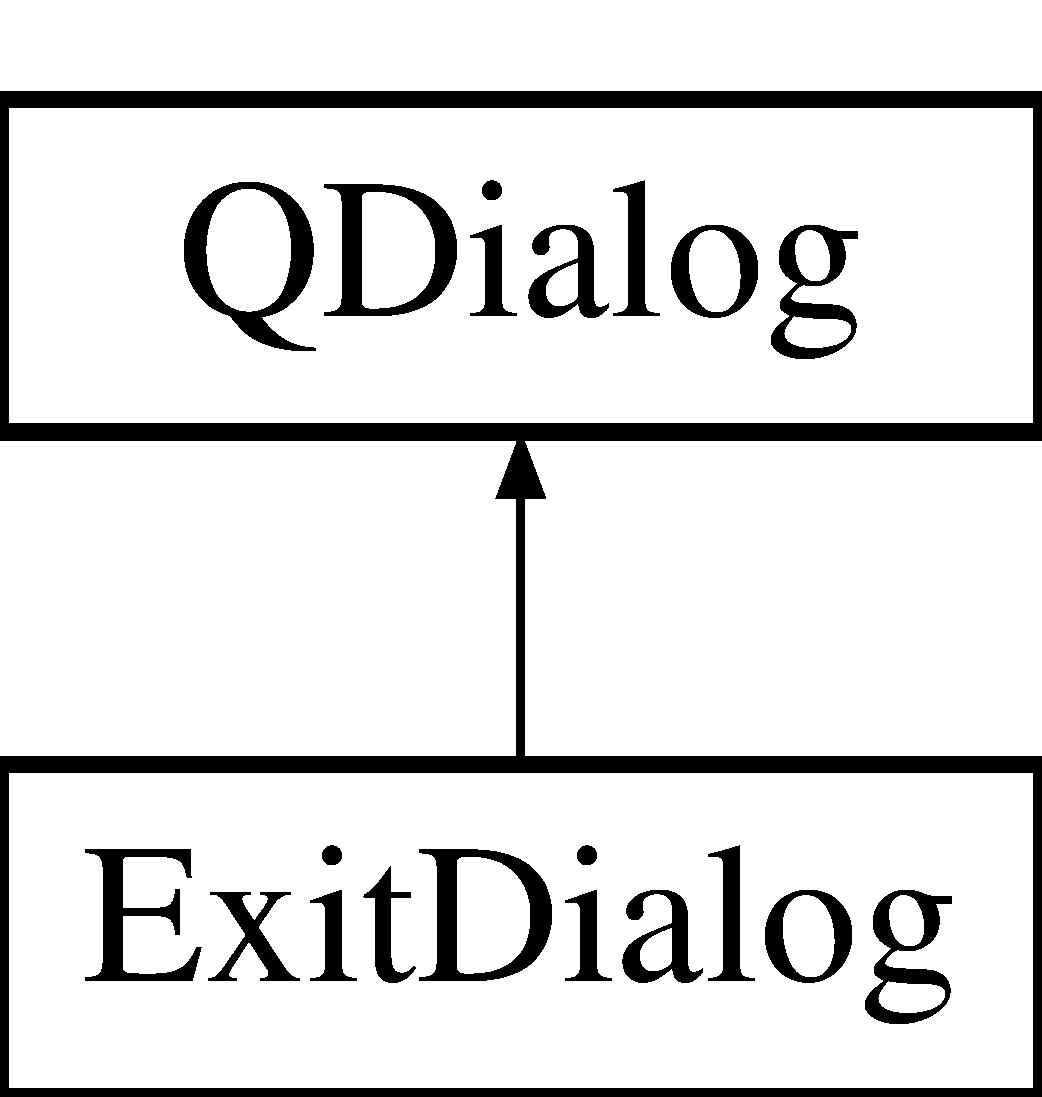
\includegraphics[height=2.000000cm]{classExitDialog}
\end{center}
\end{figure}
\subsubsection*{Public Types}
\begin{DoxyCompactItemize}
\item 
enum \mbox{\hyperlink{classExitDialog_ad0d825dce42ecd6e8827f1b6f7167dcb}{Exit\+Code\+\_\+}} \{ \begin{DoxyParamCaption}
\item{ \mbox{\hyperlink{classExitDialog_ad0d825dce42ecd6e8827f1b6f7167dcba518a5489dfa28d18da63778459d52422}{Continue}}, }
\item{ \mbox{\hyperlink{classExitDialog_ad0d825dce42ecd6e8827f1b6f7167dcba0a0f0dc1154f9163e8ce72beea39ff29}{Log\+Out}}, }
\item{ \mbox{\hyperlink{classExitDialog_ad0d825dce42ecd6e8827f1b6f7167dcba2f33cdc04de1ce7953f7aa2abf1be566}{Shutdown}}, }
\item{ \mbox{\hyperlink{classExitDialog_ad0d825dce42ecd6e8827f1b6f7167dcbacd982ca18a78d15196869e96823cd28d}{Exit\+From\+Program}}, }
\item{ \mbox{\hyperlink{classExitDialog_ad0d825dce42ecd6e8827f1b6f7167dcba7be72257e0efaee3c5e707be33bf2399}{Reprogram\+Machine}}, }
\item{ \mbox{\hyperlink{classExitDialog_ad0d825dce42ecd6e8827f1b6f7167dcbae5cc24226e0defe8868759aa87d8c11f}{Service\+Mode}}, }
\item{ \mbox{\hyperlink{classExitDialog_ad0d825dce42ecd6e8827f1b6f7167dcba5232255eabee8632a156274e921ceb69}{Restart\+Program}}, }
\item{ \mbox{\hyperlink{classExitDialog_ad0d825dce42ecd6e8827f1b6f7167dcba6237a611a5ea7749a7f7a6d7b72a1906}{Restart\+Machine}}}
\end{DoxyParamCaption}\}

\item 
typedef enum \mbox{\hyperlink{classExitDialog_ad0d825dce42ecd6e8827f1b6f7167dcb}{Exit\+Dialog\+::\+Exit\+Code\+\_\+}} \mbox{\hyperlink{classExitDialog_a750dfbbef3dec32bec821122ee7b910c}{Exit\+Code}}
\end{DoxyCompactItemize}
\subsubsection*{Public Member Functions}
\begin{DoxyCompactItemize}
\item 
\mbox{\hyperlink{classExitDialog_aa1b3d3b53b599a47b2c7d70d04ec4668}{Exit\+Dialog}} (Q\+Widget $\ast$parent=0)
\item 
\mbox{\hyperlink{classExitDialog_ae009cbdbc1b06410845a1afe2d518149}{$\sim$\+Exit\+Dialog}} ()
\item 
void \mbox{\hyperlink{classExitDialog_ab44c70526c323e87ee0b3e9e3daad41a}{set\+Log\+Out\+En}} (bool en)
\end{DoxyCompactItemize}
\subsubsection*{Static Public Member Functions}
\begin{DoxyCompactItemize}
\item 
static \mbox{\hyperlink{classExitDialog_a750dfbbef3dec32bec821122ee7b910c}{Exit\+Code}} \mbox{\hyperlink{classExitDialog_a8c287b8910a1e54c9fed6dd172fbd134}{try\+Exit}} (Q\+Widget $\ast$parent, bool log\+Out\+En=false)
\end{DoxyCompactItemize}
\subsubsection*{Protected Member Functions}
\begin{DoxyCompactItemize}
\item 
void \mbox{\hyperlink{classExitDialog_ad39269ff91b1b949ab12c8ecbcefa6f6}{show\+Event}} (Q\+Show\+Event $\ast$ev)
\item 
void \mbox{\hyperlink{classExitDialog_a460c6fce45208626b1ec54f7ed9e0629}{change\+Event}} (Q\+Event $\ast$event)
\end{DoxyCompactItemize}
\subsubsection*{Private Slots}
\begin{DoxyCompactItemize}
\item 
void \mbox{\hyperlink{classExitDialog_a007aae536da00aa771afecec4222d54e}{on\+\_\+p\+Button\+Turn\+Off\+\_\+clicked}} ()
\item 
void \mbox{\hyperlink{classExitDialog_a113e0571b5d73536f9d2c339963959f3}{on\+\_\+p\+Button\+Restart\+App\+\_\+clicked}} ()
\item 
void \mbox{\hyperlink{classExitDialog_a6c464f98d852bc55a7c088b7e3da9d07}{on\+\_\+p\+Button\+Rastart\+All\+\_\+clicked}} ()
\item 
void \mbox{\hyperlink{classExitDialog_a19cd3597771722ecdca6ce177c3d5406}{on\+\_\+p\+Button\+Service\+Mode\+\_\+clicked}} ()
\item 
void \mbox{\hyperlink{classExitDialog_a57bfa16aefc0c094bb04f2fa5a1882c6}{on\+\_\+p\+Button\+Exit\+App\+\_\+clicked}} ()
\item 
void \mbox{\hyperlink{classExitDialog_ab63b993dd9bc432cf549dd854050aa75}{on\+\_\+p\+Button\+Reprogram\+\_\+clicked}} ()
\item 
void \mbox{\hyperlink{classExitDialog_a8032c8cae9a0c12dd976fa30426bb629}{on\+\_\+p\+Button\+Log\+Out\+\_\+clicked}} ()
\item 
void \mbox{\hyperlink{classExitDialog_ad869a166c6bc6746f49b7ad311d7023a}{on\+\_\+push\+Button\+Cancel\+\_\+clicked}} ()
\end{DoxyCompactItemize}
\subsubsection*{Private Attributes}
\begin{DoxyCompactItemize}
\item 
\mbox{\hyperlink{classExitDialog_a750dfbbef3dec32bec821122ee7b910c}{Exit\+Code}} \mbox{\hyperlink{classExitDialog_adff4059e3ad467576437361b8f8518c0}{exit\+Code}}
\item 
Ui\+::\+Exit\+Dialog $\ast$ \mbox{\hyperlink{classExitDialog_a2d2914db33580192188032e15348594e}{ui}}
\end{DoxyCompactItemize}


\subsubsection{Member Typedef Documentation} \mbox{\Hypertarget{classExitDialog_a750dfbbef3dec32bec821122ee7b910c}\label{classExitDialog_a750dfbbef3dec32bec821122ee7b910c}}  \index{Exit\+Dialog@{Exit\+Dialog}!Exit\+Code@{Exit\+Code}} \index{Exit\+Code@{Exit\+Code}!Exit\+Dialog@{Exit\+Dialog}}
\paragraph{\texorpdfstring{Exit\+Code}{ExitCode}}
{\footnotesize\ttfamily typedef enum \mbox{\hyperlink{classExitDialog_ad0d825dce42ecd6e8827f1b6f7167dcb}{Exit\+Dialog\+::\+Exit\+Code\+\_\+}} \mbox{\hyperlink{classExitDialog_a750dfbbef3dec32bec821122ee7b910c}{Exit\+Dialog\+::\+Exit\+Code}}} - type of variable which will be returned from function \mbox{\hyperlink{classExitDialog_a8c287b8910a1e54c9fed6dd172fbd134}{try\+Exit}}. Created just for good code look.

\subsubsection{Member Enumeration Documentation}
\mbox{\Hypertarget{classExitDialog_ad0d825dce42ecd6e8827f1b6f7167dcb}\label{classExitDialog_ad0d825dce42ecd6e8827f1b6f7167dcb}} 
\index{Exit\+Dialog@{Exit\+Dialog}!Exit\+Code\+\_\+@{Exit\+Code\+\_\+}}
\index{Exit\+Code\+\_\+@{Exit\+Code\+\_\+}!Exit\+Dialog@{Exit\+Dialog}}
\paragraph{\texorpdfstring{Exit\+Code\+\_\+}{ExitCode\_}}
{\footnotesize\ttfamily enum \mbox{\hyperlink{classExitDialog_ad0d825dce42ecd6e8827f1b6f7167dcb}{Exit\+Dialog\+::\+Exit\+Code\+\_\+}}} - created for \mbox{\hyperlink{classExitDialog_ad0d825dce42ecd6e8827f1b6f7167dcb}{Exit\+Dialog\+::\+Exit\+Code\+\_\+}}

\begin{DoxyEnumFields}{Enumerator}
\raisebox{\heightof{T}}[0pt][0pt]{\index{Continue@{Continue}!Exit\+Dialog@{Exit\+Dialog}}\index{Exit\+Dialog@{Exit\+Dialog}!Continue@{Continue}}}\mbox{\Hypertarget{classExitDialog_ad0d825dce42ecd6e8827f1b6f7167dcba518a5489dfa28d18da63778459d52422}\label{classExitDialog_ad0d825dce42ecd6e8827f1b6f7167dcba518a5489dfa28d18da63778459d52422}} 
Continue&Flag to continue work without any changes. \mbox{\hyperlink{classExitDialog_a750dfbbef3dec32bec821122ee7b910c}{Exit\+Code}}\\
\hline

\raisebox{\heightof{T}}[0pt][0pt]{\index{Log\+Out@{Log\+Out}!Exit\+Dialog@{Exit\+Dialog}}\index{Exit\+Dialog@{Exit\+Dialog}!Log\+Out@{Log\+Out}}}\mbox{\Hypertarget{classExitDialog_ad0d825dce42ecd6e8827f1b6f7167dcba0a0f0dc1154f9163e8ce72beea39ff29}\label{classExitDialog_ad0d825dce42ecd6e8827f1b6f7167dcba0a0f0dc1154f9163e8ce72beea39ff29}} 
Log\+Out&Flag to change user.\\
\hline

\raisebox{\heightof{T}}[0pt][0pt]{\index{Shutdown@{Shutdown}!Exit\+Dialog@{Exit\+Dialog}}\index{Exit\+Dialog@{Exit\+Dialog}!Shutdown@{Shutdown}}}\mbox{\Hypertarget{classExitDialog_ad0d825dce42ecd6e8827f1b6f7167dcba2f33cdc04de1ce7953f7aa2abf1be566}\label{classExitDialog_ad0d825dce42ecd6e8827f1b6f7167dcba2f33cdc04de1ce7953f7aa2abf1be566}} 
Shutdown& Flag to exit from program and send shutdown signal to operating system.\\
\hline

\raisebox{\heightof{T}}[0pt][0pt]{\index{Exit\+From\+Program@{Exit\+From\+Program}!Exit\+Dialog@{Exit\+Dialog}}\index{Exit\+Dialog@{Exit\+Dialog}!Exit\+From\+Program@{Exit\+From\+Program}}}\mbox{\Hypertarget{classExitDialog_ad0d825dce42ecd6e8827f1b6f7167dcbacd982ca18a78d15196869e96823cd28d}\label{classExitDialog_ad0d825dce42ecd6e8827f1b6f7167dcbacd982ca18a78d15196869e96823cd28d}} 
Exit\+From\+Program&Flag to exit from program and go to graphical user interface of operating system.\\
\hline

\raisebox{\heightof{T}}[0pt][0pt]{\index{Reprogram\+Machine@{Reprogram\+Machine}!Exit\+Dialog@{Exit\+Dialog}}\index{Exit\+Dialog@{Exit\+Dialog}!Reprogram\+Machine@{Reprogram\+Machine}}}\mbox{\Hypertarget{classExitDialog_ad0d825dce42ecd6e8827f1b6f7167dcba7be72257e0efaee3c5e707be33bf2399}\label{classExitDialog_ad0d825dce42ecd6e8827f1b6f7167dcba7be72257e0efaee3c5e707be33bf2399}} 
Reprogram\+Machine&Send signal disconnect serial port and connect with other parameters.
After that open {\mbox{\hyperlink{classReprogramDialog}{Reprogram\+Dialog}} class object (or create and open it).}\\
\hline

\raisebox{\heightof{T}}[0pt][0pt]{\index{Service\+Mode@{Service\+Mode}!Exit\+Dialog@{Exit\+Dialog}}\index{Exit\+Dialog@{Exit\+Dialog}!Service\+Mode@{Service\+Mode}}}\mbox{\Hypertarget{classExitDialog_ad0d825dce42ecd6e8827f1b6f7167dcbae5cc24226e0defe8868759aa87d8c11f}\label{classExitDialog_ad0d825dce42ecd6e8827f1b6f7167dcbae5cc24226e0defe8868759aa87d8c11f}} 
Service\+Mode&Flag to disconnect serial port connection (break data line between PC and master board) to give possibility press buttons without machine moving. \\
\hline

\raisebox{\heightof{T}}[0pt][0pt]{\index{Restart\+Program@{Restart\+Program}!Exit\+Dialog@{Exit\+Dialog}}\index{Exit\+Dialog@{Exit\+Dialog}!Restart\+Program@{Restart\+Program}}}\mbox{\Hypertarget{classExitDialog_ad0d825dce42ecd6e8827f1b6f7167dcba5232255eabee8632a156274e921ceb69}\label{classExitDialog_ad0d825dce42ecd6e8827f1b6f7167dcba5232255eabee8632a156274e921ceb69}} 
Restart\+Program&Flag to re-initialization of program.\\
\hline

\raisebox{\heightof{T}}[0pt][0pt]{\index{Restart\+Machine@{Restart\+Machine}!Exit\+Dialog@{Exit\+Dialog}}\index{Exit\+Dialog@{Exit\+Dialog}!Restart\+Machine@{Restart\+Machine}}}\mbox{\Hypertarget{classExitDialog_ad0d825dce42ecd6e8827f1b6f7167dcba6237a611a5ea7749a7f7a6d7b72a1906}\label{classExitDialog_ad0d825dce42ecd6e8827f1b6f7167dcba6237a611a5ea7749a7f7a6d7b72a1906}} 
Restart\+Machine&Flag to exit from program and send restart signal to operating system. After system restart program will start in usual mode.\\
\hline

\end{DoxyEnumFields}

\subsubsection{Constructor \& Destructor Documentation}
\mbox{\Hypertarget{classExitDialog_aa1b3d3b53b599a47b2c7d70d04ec4668}\label{classExitDialog_aa1b3d3b53b599a47b2c7d70d04ec4668}} \index{Exit\+Dialog@{Exit\+Dialog}!Exit\+Dialog@{Exit\+Dialog}} \index{Exit\+Dialog@{Exit\+Dialog}!Exit\+Dialog@{Exit\+Dialog}}
\paragraph{\texorpdfstring{Exit\+Dialog()}{ExitDialog()}}
{\footnotesize\ttfamily Exit\+Dialog\+::\+Exit\+Dialog (\begin{DoxyParamCaption}\item[{Q\+Widget $\ast$}]{parent = {\ttfamily 0} }\end{DoxyParamCaption}){\ttfamily [explicit]}}
\mbox{\Hypertarget{classExitDialog_ae009cbdbc1b06410845a1afe2d518149}\label{classExitDialog_ae009cbdbc1b06410845a1afe2d518149}} 
\index{Exit\+Dialog@{Exit\+Dialog}!````~Exit\+Dialog@{$\sim$\+Exit\+Dialog}}
\index{````~Exit\+Dialog@{$\sim$\+Exit\+Dialog}!Exit\+Dialog@{Exit\+Dialog}}
\paragraph{\texorpdfstring{$\sim$\+Exit\+Dialog()}{~ExitDialog()}}
{\footnotesize\ttfamily Exit\+Dialog\+::$\sim$\+Exit\+Dialog (\begin{DoxyParamCaption}{ }\end{DoxyParamCaption})}\\

\subsubsection{Member Function Documentation}
\mbox{\Hypertarget{classExitDialog_a460c6fce45208626b1ec54f7ed9e0629}\label{classExitDialog_a460c6fce45208626b1ec54f7ed9e0629}} 
\index{Exit\+Dialog@{Exit\+Dialog}!change\+Event@{change\+Event}}
\index{change\+Event@{change\+Event}!Exit\+Dialog@{Exit\+Dialog}}
{\footnotesize\ttfamily void Exit\+Dialog\+::\texorpdfstring{change\+Event()}{changeEvent()} (\begin{DoxyParamCaption}\item[{Q\+Event $\ast$}]{event }\end{DoxyParamCaption}){\ttfamily [protected]}} - Reimplementation of default event for Q\+Dialog to enable user interface translation. Function called automatically.
\begin{center}	\line(1,0){450} \end{center}
All function in itemizer are called by click signals of appropriate buttons and assigns appropriate to button (function) name value (from \hyperlink{classExitDialog_ad0d825dce42ecd6e8827f1b6f7167dcb}{Exit\+Code\+\_\+} enumerator) to \hyperlink{classExitDialog_adff4059e3ad467576437361b8f8518c0}{exit\+Code} variable. That variable will return by \hyperlink{classExitDialog_a8c287b8910a1e54c9fed6dd172fbd134}{try\+Exit}(...) function.
\begin{DoxyCompactItemize}
\item \mbox{\Hypertarget{classExitDialog_a57bfa16aefc0c094bb04f2fa5a1882c6}\label{classExitDialog_a57bfa16aefc0c094bb04f2fa5a1882c6}} 
\index{Exit\+Dialog@{Exit\+Dialog}!on\+\_\+p\+Button\+Exit\+App\+\_\+clicked@{on\+\_\+p\+Button\+Exit\+App\+\_\+clicked}}
\index{on\+\_\+p\+Button\+Exit\+App\+\_\+clicked@{on\+\_\+p\+Button\+Exit\+App\+\_\+clicked}!Exit\+Dialog@{Exit\+Dialog}}
{\footnotesize\ttfamily void Exit\+Dialog\+::on\+\_\+p\+Button\+Exit\+App\+\_\+clicked (\begin{DoxyParamCaption}{ }\end{DoxyParamCaption}){\ttfamily [private]}, {\ttfamily [slot]}}
\item \mbox{\Hypertarget{classExitDialog_a8032c8cae9a0c12dd976fa30426bb629}\label{classExitDialog_a8032c8cae9a0c12dd976fa30426bb629}} 
\index{Exit\+Dialog@{Exit\+Dialog}!on\+\_\+p\+Button\+Log\+Out\+\_\+clicked@{on\+\_\+p\+Button\+Log\+Out\+\_\+clicked}}
\index{on\+\_\+p\+Button\+Log\+Out\+\_\+clicked@{on\+\_\+p\+Button\+Log\+Out\+\_\+clicked}!Exit\+Dialog@{Exit\+Dialog}}
{\footnotesize\ttfamily void Exit\+Dialog\+::\texorpdfstring{on\+\_\+p\+Button\+Log\+Out\+\_\+clicked}{on\_pButtonLogOut\_clicked} (\begin{DoxyParamCaption}{ }\end{DoxyParamCaption}){\ttfamily [private]}, {\ttfamily [slot]}}
\item \mbox{\Hypertarget{classExitDialog_a6c464f98d852bc55a7c088b7e3da9d07}\label{classExitDialog_a6c464f98d852bc55a7c088b7e3da9d07}} 
\index{Exit\+Dialog@{Exit\+Dialog}!on\+\_\+p\+Button\+Rastart\+All\+\_\+clicked@{on\+\_\+p\+Button\+Rastart\+All\+\_\+clicked}}
\index{on\+\_\+p\+Button\+Rastart\+All\+\_\+clicked@{on\+\_\+p\+Button\+Rastart\+All\+\_\+clicked}!Exit\+Dialog@{Exit\+Dialog}}
{\footnotesize\ttfamily void Exit\+Dialog\+::\texorpdfstring{on\+\_\+p\+Button\+Rastart\+All\+\_\+clicked}{on\_pButtonRastartAll\_clicked} (\begin{DoxyParamCaption}{ }\end{DoxyParamCaption}){\ttfamily [private]}, {\ttfamily [slot]}}
\item \mbox{\Hypertarget{classExitDialog_ab63b993dd9bc432cf549dd854050aa75}\label{classExitDialog_ab63b993dd9bc432cf549dd854050aa75}} 
\index{Exit\+Dialog@{Exit\+Dialog}!on\+\_\+p\+Button\+Reprogram\+\_\+clicked@{on\+\_\+p\+Button\+Reprogram\+\_\+clicked}}
\index{on\+\_\+p\+Button\+Reprogram\+\_\+clicked@{on\+\_\+p\+Button\+Reprogram\+\_\+clicked}!Exit\+Dialog@{Exit\+Dialog}}
{\footnotesize\ttfamily void Exit\+Dialog\+::\texorpdfstring{on\+\_\+p\+Button\+Reprogram\+\_\+clicked}{on\_pButtonReprogram\_clicked} (\begin{DoxyParamCaption}{ }\end{DoxyParamCaption}){\ttfamily [private]}, {\ttfamily [slot]}}
\item \mbox{\Hypertarget{classExitDialog_a113e0571b5d73536f9d2c339963959f3}\label{classExitDialog_a113e0571b5d73536f9d2c339963959f3}} 
\index{Exit\+Dialog@{Exit\+Dialog}!on\+\_\+p\+Button\+Restart\+App\+\_\+clicked@{on\+\_\+p\+Button\+Restart\+App\+\_\+clicked}}
\index{on\+\_\+p\+Button\+Restart\+App\+\_\+clicked@{on\+\_\+p\+Button\+Restart\+App\+\_\+clicked}!Exit\+Dialog@{Exit\+Dialog}}
{\footnotesize\ttfamily void Exit\+Dialog\+::\texorpdfstring{on\+\_\+p\+Button\+Restart\+App\+\_\+clicked}{on\_pButtonRestartApp\_clicked} (\begin{DoxyParamCaption}{ }\end{DoxyParamCaption}){\ttfamily [private]}, {\ttfamily [slot]}}
\item \mbox{\Hypertarget{classExitDialog_a19cd3597771722ecdca6ce177c3d5406}\label{classExitDialog_a19cd3597771722ecdca6ce177c3d5406}} 
\index{Exit\+Dialog@{Exit\+Dialog}!on\+\_\+p\+Button\+Service\+Mode\+\_\+clicked@{on\+\_\+p\+Button\+Service\+Mode\+\_\+clicked}}
\index{on\+\_\+p\+Button\+Service\+Mode\+\_\+clicked@{on\+\_\+p\+Button\+Service\+Mode\+\_\+clicked}!Exit\+Dialog@{Exit\+Dialog}}
{\footnotesize\ttfamily void Exit\+Dialog\+::\texorpdfstring{on\+\_\+p\+Button\+Service\+Mode\+\_\+clicked}{on\_pButtonServiceMode\_clicked} (\begin{DoxyParamCaption}{ }\end{DoxyParamCaption}){\ttfamily [private]}, {\ttfamily [slot]}}
\item \mbox{\Hypertarget{classExitDialog_a007aae536da00aa771afecec4222d54e}\label{classExitDialog_a007aae536da00aa771afecec4222d54e}} 
\index{Exit\+Dialog@{Exit\+Dialog}!on\+\_\+p\+Button\+Turn\+Off\+\_\+clicked@{on\+\_\+p\+Button\+Turn\+Off\+\_\+clicked}}
\index{on\+\_\+p\+Button\+Turn\+Off\+\_\+clicked@{on\+\_\+p\+Button\+Turn\+Off\+\_\+clicked}!Exit\+Dialog@{Exit\+Dialog}}
{\footnotesize\ttfamily void Exit\+Dialog\+::\texorpdfstring{on\+\_\+p\+Button\+Turn\+Off\+\_\+clicked}{on\_pButtonTurnOff\_clicked} (\begin{DoxyParamCaption}{ }\end{DoxyParamCaption}){\ttfamily [private]}, {\ttfamily [slot]}}
\item \mbox{\Hypertarget{classExitDialog_ad869a166c6bc6746f49b7ad311d7023a}\label{classExitDialog_ad869a166c6bc6746f49b7ad311d7023a}} 
\index{Exit\+Dialog@{Exit\+Dialog}!on\+\_\+push\+Button\+Cancel\+\_\+clicked@{on\+\_\+push\+Button\+Cancel\+\_\+clicked}}
\index{on\+\_\+push\+Button\+Cancel\+\_\+clicked@{on\+\_\+push\+Button\+Cancel\+\_\+clicked}!Exit\+Dialog@{Exit\+Dialog}}
{\footnotesize\ttfamily void Exit\+Dialog\+::\texorpdfstring{on\+\_\+push\+Button\+Cancel\+\_\+clicked}{on\_pushButtonCancel\_clicked} (\begin{DoxyParamCaption}{ }\end{DoxyParamCaption}){\ttfamily [private]}, {\ttfamily [slot]}}
\end{DoxyCompactItemize}
\begin{center}	\line(1,0){450} \end{center}
\mbox{\Hypertarget{classExitDialog_ab44c70526c323e87ee0b3e9e3daad41a}\label{classExitDialog_ab44c70526c323e87ee0b3e9e3daad41a}} 
\index{Exit\+Dialog@{Exit\+Dialog}!set\+Log\+Out\+En@{set\+Log\+Out\+En}}
\index{set\+Log\+Out\+En@{set\+Log\+Out\+En}!Exit\+Dialog@{Exit\+Dialog}}
{\footnotesize\ttfamily void Exit\+Dialog\+::\texorpdfstring{set\+Log\+Out\+En()}{setLogOutEn()} (\begin{DoxyParamCaption}\item[{bool}]{en }\end{DoxyParamCaption})}
 - Function to enable or disable \textit{pButtonLogOut} at exit dialog. Call with \textit{true} value to show button and with \textit{false} to hide it.

\mbox{\Hypertarget{classExitDialog_ad39269ff91b1b949ab12c8ecbcefa6f6}\label{classExitDialog_ad39269ff91b1b949ab12c8ecbcefa6f6}} 
\index{Exit\+Dialog@{Exit\+Dialog}!show\+Event@{show\+Event}}
\index{show\+Event@{show\+Event}!Exit\+Dialog@{Exit\+Dialog}}
{\footnotesize\ttfamily void Exit\+Dialog\+::\texorpdfstring{show\+Event()}{showEvent()} (\begin{DoxyParamCaption}\item[{Q\+Show\+Event $\ast$}]{ev }\end{DoxyParamCaption}){\ttfamily [protected]}} - Reimplementation of default event for Q\+Dialog. In this reimplementation added hiding (or showing) buttons, which are not available for all users. Function called automatically on every window call.

\mbox{\Hypertarget{classExitDialog_a8c287b8910a1e54c9fed6dd172fbd134}\label{classExitDialog_a8c287b8910a1e54c9fed6dd172fbd134}} 
\index{Exit\+Dialog@{Exit\+Dialog}!try\+Exit@{try\+Exit}}
\index{try\+Exit@{try\+Exit}!Exit\+Dialog@{Exit\+Dialog}}
{\footnotesize\ttfamily \mbox{\hyperlink{classExitDialog_a750dfbbef3dec32bec821122ee7b910c}{Exit\+Dialog\+::\+Exit\+Code}} Exit\+Dialog\+::\texorpdfstring{try\+Exit}{tryExit} (\begin{DoxyParamCaption}\item[{Q\+Widget $\ast$}]{parent,  }\item[{bool}]{log\+Out\+En = {\ttfamily false} }\end{DoxyParamCaption}){\ttfamily [static]}} - static function to call exit dialog end get \hyperlink{classExitDialog_a750dfbbef3dec32bec821122ee7b910c}{Exit\+Dialog\+::\+Exit\+Code}.


\subsubsection{Member Data Documentation}
\mbox{\Hypertarget{classExitDialog_adff4059e3ad467576437361b8f8518c0}\label{classExitDialog_adff4059e3ad467576437361b8f8518c0}} 
\index{Exit\+Dialog@{Exit\+Dialog}!exit\+Code@{exit\+Code}}
\index{exit\+Code@{exit\+Code}!Exit\+Dialog@{Exit\+Dialog}}
{\footnotesize\ttfamily \mbox{\hyperlink{classExitDialog_a750dfbbef3dec32bec821122ee7b910c}{\texorpdfstring{exit\+Code}{exitCode}}} Exit\+Dialog\+::exit\+Code{\ttfamily [private]}} 

The documentation for this class was generated from the following files\+:\begin{DoxyCompactItemize}
\item 
\mbox{\hyperlink{exitdialog_8h}{exitdialog.\+h}}\item 
\mbox{\hyperlink{exitdialog_8cpp}{exitdialog.\+cpp}}\end{DoxyCompactItemize}
\newpage
\hypertarget{classGeneralSettingDialog}{}\subsection{General\+Setting\+Dialog Class Reference}
\label{classGeneralSettingDialog}\index{General\+Setting\+Dialog@{General\+Setting\+Dialog}}


{\ttfamily \#include $<$generalsettingdialog.\+h$>$}

Inheritance diagram for General\+Setting\+Dialog\+:\begin{figure}[H]
\begin{center}
\leavevmode
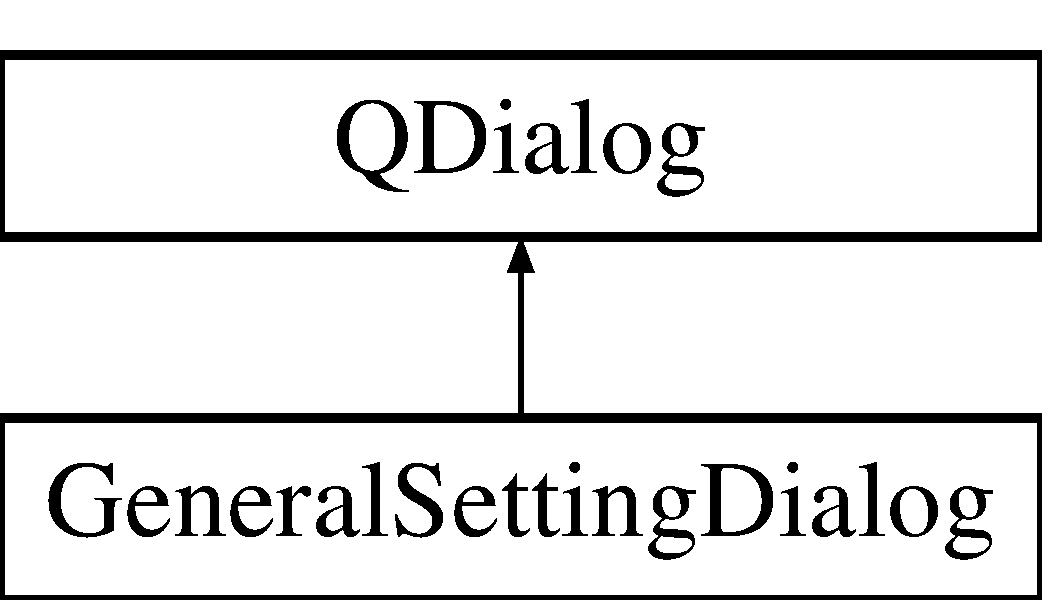
\includegraphics[height=2.000000cm]{classGeneralSettingDialog}
\end{center}
\end{figure}
\subsubsection*{Signals}
\begin{DoxyCompactItemize}
\item 
void \mbox{\hyperlink{classGeneralSettingDialog_a825854c03817dfdb5b7c6185008ab620}{email\+Settings\+Changed}} (\mbox{\hyperlink{structEmailSettings}{Email\+Settings}})
\item 
void \mbox{\hyperlink{classGeneralSettingDialog_a02019fb6d81fc0e83ed6ae0ef7ef68b4}{machine\+Param\+Changed}} (Q\+Byte\+Array machine\+Pararm\+Arr)
\item 
void \mbox{\hyperlink{classGeneralSettingDialog_aef493e3f166d3bd7cb982f854f29617e}{serial\+Port\+Settings\+Dialog\+Requested}} ()
\item 
void \mbox{\hyperlink{classGeneralSettingDialog_ab651d47f726e1049c0bf34e6ebcb8cf1}{style\+Changed\+Index}} (int index)
\item 
void \mbox{\hyperlink{classGeneralSettingDialog_aa0b2ee80957f63f302aa9a6ac6e13f5d}{icons\+Changed\+Index}} (int index)
\item 
void \mbox{\hyperlink{classGeneralSettingDialog_ac3d2f3477274bedf08848cc24eaece06}{lang\+Changed\+Index}} (int index)
\item 
void \mbox{\hyperlink{classGeneralSettingDialog_a8ac7f5a379cd6ec270bc98050e4c7765}{service\+Setting\+Request}} ()
\item 
void \mbox{\hyperlink{classGeneralSettingDialog_a386763acc4545a1c03542ef71601c23c}{head\+Activation\+Request}} ()
\item 
void \mbox{\hyperlink{classGeneralSettingDialog_a9bc417a43ff037b30e281e38fbc98744}{users\+Setting\+Request}} ()
\item 
void \mbox{\hyperlink{classGeneralSettingDialog_aa4bc1d43246c829906a530b5a127a417}{direction\+Changed}} (int dir)
\item 
void \mbox{\hyperlink{classGeneralSettingDialog_a3ec05b9d5bf741008ba575d408af6c04}{unload\+State\+Changed}} (bool state)
\item 
void \mbox{\hyperlink{classGeneralSettingDialog_aa381596bc44cfcaeb85a8d906b877b86}{send\+Command}} (Q\+Byte\+Array command)
\item 
void \mbox{\hyperlink{classGeneralSettingDialog_a1c6ff8e8d7b1ad5f4399942ea48dc9d8}{image\+Request}} (bool enable, bool req=false)
\end{DoxyCompactItemize}
\subsubsection*{Public Member Functions}
\begin{DoxyCompactItemize}
\item 
\mbox{\hyperlink{classGeneralSettingDialog_a04717ff5a0b42fb1ebeb5dcfc934cd83}{General\+Setting\+Dialog}} (Q\+Widget $\ast$parent=0)
\item 
\mbox{\hyperlink{classGeneralSettingDialog_a6e45c39d066344fdc3fd8556bed18cd3}{$\sim$\+General\+Setting\+Dialog}} ()
\item 
void \mbox{\hyperlink{classGeneralSettingDialog_ab9ca0f722e745c5cbf9d35c0307a2740}{set\+Icon\+Folder}} (Q\+String path)
\item 
void \mbox{\hyperlink{classGeneralSettingDialog_a418a131dbac78536218003bafc7988ae}{set\+Email\+Settings}} (\mbox{\hyperlink{structEmailSettings}{Email\+Settings}} email\+Sett)
\item 
void \mbox{\hyperlink{classGeneralSettingDialog_a62392d2454fdaf652f789792b50f9c6c}{set\+Machine\+Setting}} (\mbox{\hyperlink{classMachineSettings_a87879e13793dbc7c10d4fa18e1236751}{Machine\+Settings\+::\+Machine\+Parameters}} machine\+Param)
\item 
void \mbox{\hyperlink{classGeneralSettingDialog_a43d51bbc0d1681b933c9c630c08e88fa}{set\+Focus\+Loss\+Accept}} (bool flag)
\item 
void \mbox{\hyperlink{classGeneralSettingDialog_a73e0c08d830948be4ec0f8d3d155c5ca}{set\+Passwords}} (\mbox{\hyperlink{settings_8h_a017dd44e68049ffdd31500a8cd01ba68}{uint16\+\_\+t}} serial\+Pass, \mbox{\hyperlink{settings_8h_a017dd44e68049ffdd31500a8cd01ba68}{uint16\+\_\+t}} mail\+Pass, \mbox{\hyperlink{settings_8h_a017dd44e68049ffdd31500a8cd01ba68}{uint16\+\_\+t}} user\+Pass)
\item 
void \mbox{\hyperlink{classGeneralSettingDialog_a1746ad8d326d2adff1e8297f48119835}{set\+Style}} (Q\+String\+List st\+List, int cur\+Select, Q\+String\+List icon\+List, int icon\+Sel, bool back\+Gr\+En)
\item 
void \mbox{\hyperlink{classGeneralSettingDialog_a6ba230057e081886f781539e4464ba99}{set\+Lang\+List}} (Q\+String\+List lang\+List, int cur\+Select)
\item 
void \mbox{\hyperlink{classGeneralSettingDialog_a947b14b03ff390dc93d9d3d5cc8ef962}{show\+Port\+Info}} (\mbox{\hyperlink{structComSettings}{Com\+Settings}} com\+Sett)
\end{DoxyCompactItemize}
\subsubsection*{Protected Member Functions}
\begin{DoxyCompactItemize}
\item 
bool \mbox{\hyperlink{classGeneralSettingDialog_ab8a8c443ea722ca23024025efbcfa768}{event}} (Q\+Event $\ast$e)
\item 
bool \mbox{\hyperlink{classGeneralSettingDialog_a2e5fc0aa0ac5f04fcfb032d65c1893a4}{event\+Filter}} (Q\+Object $\ast$watched, Q\+Event $\ast$\mbox{\hyperlink{classGeneralSettingDialog_ab8a8c443ea722ca23024025efbcfa768}{event}})
\item 
void \mbox{\hyperlink{classGeneralSettingDialog_a023c0f13fee36afb784b0ac7507f0fd2}{show\+Event}} (Q\+Show\+Event $\ast$ev)
\item 
void \mbox{\hyperlink{classGeneralSettingDialog_aecac66d55350cfbe21c6bac6f5476099}{change\+Event}} (Q\+Event $\ast$\mbox{\hyperlink{classGeneralSettingDialog_ab8a8c443ea722ca23024025efbcfa768}{event}})
\end{DoxyCompactItemize}
\subsubsection*{Private Slots}
\begin{DoxyCompactItemize}
\item 
void \mbox{\hyperlink{classGeneralSettingDialog_a8f189ce9494b6c5488f8a2be4c792f6a}{accept}} ()
\item 
void \mbox{\hyperlink{classGeneralSettingDialog_a2f4495a0f2911e41d3eaeec00949bde8}{reject}} ()
\item 
void \mbox{\hyperlink{classGeneralSettingDialog_a53e28908636048d815628b85dcaaca4c}{lock\+Unlock\+Email}} ()
\item 
void \mbox{\hyperlink{classGeneralSettingDialog_a15e7d8a20dbb83ea3ee46dd57446ec36}{hide\+Show\+Password}} ()
\item 
void \mbox{\hyperlink{classGeneralSettingDialog_aafd1047488eb1f024f0b572a95c454ad}{event\+Filter\+Setup}} ()
\item 
void \mbox{\hyperlink{classGeneralSettingDialog_afd7ce89c9dde6f411472da4e413475ec}{change\+Serial\+Port\+Settings\+Clicked}} ()
\item 
void \mbox{\hyperlink{classGeneralSettingDialog_ad5275b9ede5252e57d4b6a44eb771a04}{change\+Service\+State\+Clicked}} ()
\item 
void \mbox{\hyperlink{classGeneralSettingDialog_abfa33957c880ab0172b2ee30e848f6bd}{user\+Setting\+Clicked}} ()
\item 
void \mbox{\hyperlink{classGeneralSettingDialog_ac250bc3aba6c2e247d26f5ece4b32af7}{style\+Changed}} (int index)
\item 
void \mbox{\hyperlink{classGeneralSettingDialog_a6907e319fa3cedb66f4645cd0f3ad676}{icon\+Changed}} (int index)
\item 
void \mbox{\hyperlink{classGeneralSettingDialog_a80bce87bcafdf14692465fc5ae181a4c}{lang\+Changed}} (int index)
\item 
void \mbox{\hyperlink{classGeneralSettingDialog_a67274a86c828985ee88c055de4d2bce5}{change\+Direction}} ()
\item 
void \mbox{\hyperlink{classGeneralSettingDialog_aada0bfc2b43de3d88d705194362a769d}{change\+Cycles\+State}} ()
\item 
void \mbox{\hyperlink{classGeneralSettingDialog_acfb5eb53ac65d1aa5f037e88d91fa7e8}{use\+Unload\+State\+Changed}} ()
\item 
void \mbox{\hyperlink{classGeneralSettingDialog_ab986e75742799d02b8268d9743a422d6}{head\+Count\+Changed}} (double arg1)
\item 
void \mbox{\hyperlink{classGeneralSettingDialog_a30243bd5ab4a0e2016b8a481504ccb62}{machine\+Type\+Changet}} (int index)
\item 
void \mbox{\hyperlink{classGeneralSettingDialog_a9b1d7ada4c3dccc4c3a516b69dd714b9}{warning\+Time\+Changed}} (double arg1)
\item 
void \mbox{\hyperlink{classGeneralSettingDialog_a8b72a332c8c98096b1f15cf1fd6b01be}{on\+\_\+p\+Button\+Heads\+Activation\+\_\+clicked}} ()
\item 
void \mbox{\hyperlink{classGeneralSettingDialog_a2fbe72c63737ff21b4780013a0cbe35a}{on\+\_\+check\+Box\+Use\+Backgr\+\_\+clicked}} ()
\item 
void \mbox{\hyperlink{classGeneralSettingDialog_a28115db3d9b5197703e789ac6cac8c9a}{on\+\_\+p\+Button\+Select\+Img\+\_\+clicked}} ()
\end{DoxyCompactItemize}
\subsubsection*{Private Attributes}
\begin{DoxyCompactItemize}
\item 
Ui\+::\+General\+Setting\+Dialog $\ast$ \mbox{\hyperlink{classGeneralSettingDialog_a2985b76397645d9f6d0cd00bccb337dc}{ui}}
\item 
\mbox{\hyperlink{classMachineSettings_a87879e13793dbc7c10d4fa18e1236751}{Machine\+Settings\+::\+Machine\+Parameters}} \mbox{\hyperlink{classGeneralSettingDialog_a61add6dfb9616d6309206cda8af09899}{machine\+Param\+Gl}}
\item 
bool \mbox{\hyperlink{classGeneralSettingDialog_a73bdef0f355634453cce0f75ccf0c173}{accept\+On\+Deactilation\+En}}
\item 
bool \mbox{\hyperlink{classGeneralSettingDialog_a63cb4068f4e5f307a5c09bc0806d0345}{accept\+Enable}}
\item 
bool \mbox{\hyperlink{classGeneralSettingDialog_acc7b6201adba8b9e35dc675d212047cc}{loged\+In\+Serial}}
\item 
bool \mbox{\hyperlink{classGeneralSettingDialog_aed1425f6474086f9fc89cbe24e6f3409}{loged\+In\+Mail}}
\item 
bool \mbox{\hyperlink{classGeneralSettingDialog_a21fbb6d0ad1c22a90032d3fed66a247f}{loged\+In\+User\+Sett}}
\item 
\mbox{\hyperlink{settings_8h_a017dd44e68049ffdd31500a8cd01ba68}{uint16\+\_\+t}} \mbox{\hyperlink{classGeneralSettingDialog_abaef63e383cc4c45581e16f85fd88a77}{serial\+Password}}
\item 
\mbox{\hyperlink{settings_8h_a017dd44e68049ffdd31500a8cd01ba68}{uint16\+\_\+t}} \mbox{\hyperlink{classGeneralSettingDialog_a214b0ddac5d79aee98e6c6e81fb45380}{mail\+Password}}
\item 
\mbox{\hyperlink{settings_8h_a017dd44e68049ffdd31500a8cd01ba68}{uint16\+\_\+t}} \mbox{\hyperlink{classGeneralSettingDialog_a365c466e185f88bad08aeb6ff036c403}{users\+Password}}
\item 
Q\+Icon \mbox{\hyperlink{classGeneralSettingDialog_ab4b216b0182add4c144d933694556f40}{direction\+Icon}}
\item 
Q\+String \mbox{\hyperlink{classGeneralSettingDialog_a17784de076ae5cfae6e150736d81a9a6}{path\+Icon}}
\end{DoxyCompactItemize}


\subsubsection{Constructor \& Destructor Documentation}
\mbox{\Hypertarget{classGeneralSettingDialog_a04717ff5a0b42fb1ebeb5dcfc934cd83}\label{classGeneralSettingDialog_a04717ff5a0b42fb1ebeb5dcfc934cd83}} \index{General\+Setting\+Dialog@{General\+Setting\+Dialog}!General\+Setting\+Dialog@{General\+Setting\+Dialog}} \index{General\+Setting\+Dialog@{General\+Setting\+Dialog}!General\+Setting\+Dialog@{General\+Setting\+Dialog}}
{\footnotesize\ttfamily General\+Setting\+Dialog\+::\texorpdfstring{General\+Setting\+Dialog()}{GeneralSettingDialog()} (\begin{DoxyParamCaption}\item[{Q\+Widget $\ast$}]{parent = {\ttfamily 0} }\end{DoxyParamCaption})}{\ttfamily [explicit]} - constructor of class. Connect signals to clots, fill combo\+Boxes with data and initialize variables to zero values.

\mbox{\Hypertarget{classGeneralSettingDialog_a6e45c39d066344fdc3fd8556bed18cd3}\label{classGeneralSettingDialog_a6e45c39d066344fdc3fd8556bed18cd3}} 
\index{General\+Setting\+Dialog@{General\+Setting\+Dialog}!````~General\+Setting\+Dialog@{$\sim$\+General\+Setting\+Dialog}}
\index{````~General\+Setting\+Dialog@{$\sim$\+General\+Setting\+Dialog}!General\+Setting\+Dialog@{General\+Setting\+Dialog}}
\paragraph{\texorpdfstring{$\sim$\+General\+Setting\+Dialog()}{~GeneralSettingDialog()}}
{\footnotesize\ttfamily General\+Setting\+Dialog\+::$\sim$\+General\+Setting\+Dialog (\begin{DoxyParamCaption}{ }\end{DoxyParamCaption})} - standard destructor function.

\subsubsection{Member Function Documentation}
\mbox{\Hypertarget{classGeneralSettingDialog_a8f189ce9494b6c5488f8a2be4c792f6a}\label{classGeneralSettingDialog_a8f189ce9494b6c5488f8a2be4c792f6a}} 
\index{General\+Setting\+Dialog@{General\+Setting\+Dialog}!accept@{accept}}
\index{accept@{accept}!General\+Setting\+Dialog@{General\+Setting\+Dialog}}
{\footnotesize\ttfamily void General\+Setting\+Dialog\+::\texorpdfstring{accept}{accept} (\begin{DoxyParamCaption}{ }\end{DoxyParamCaption}){\ttfamily [private]}, {\ttfamily [slot]}} - gather \hyperlink{structEmailSettings}{Email\+Settings} and \hyperlink{classMachineSettings_a87879e13793dbc7c10d4fa18e1236751}{Machine\+Settings\+::\+Machine\+Parameters} to appropriate structures. After that function generate signals \hyperlink{classGeneralSettingDialog_a825854c03817dfdb5b7c6185008ab620}{email\+Settings\+Changed}(...) and \hyperlink{classGeneralSettingDialog_a02019fb6d81fc0e83ed6ae0ef7ef68b4}{machine\+Param\+Changed}(...) which are call appropriate function in parent object (\hyperlink{classMainWindow_a5782e86aacd3c157412821fae13c85fb}{get\+Email\+Settings}(...) and \hyperlink{classMainWindow_a2dc63192aa7ff54dfc64e8308712c287}{get\+Machine\+Param}(...)).

\mbox{\Hypertarget{classGeneralSettingDialog_aada0bfc2b43de3d88d705194362a769d}\label{classGeneralSettingDialog_aada0bfc2b43de3d88d705194362a769d}} 
\index{General\+Setting\+Dialog@{General\+Setting\+Dialog}!change\+Cycles\+State@{change\+Cycles\+State}}
\index{change\+Cycles\+State@{change\+Cycles\+State}!General\+Setting\+Dialog@{General\+Setting\+Dialog}}
{\footnotesize\ttfamily void General\+Setting\+Dialog\+::\texorpdfstring{change\+Cycles\+State}{changeCyclesState} (\begin{DoxyParamCaption}{ }\end{DoxyParamCaption}){\ttfamily [private]}, {\ttfamily [slot]}} - send command with \hyperlink{classGeneralSettingDialog_aa381596bc44cfcaeb85a8d906b877b86}{send\+Command}(...) function to turn on/off revolver function of machine and show/hide button "Cycles" on main interface (That button call \hyperlink{classCyclesDialog}{Cycles\+Dialog} class object).

\mbox{\Hypertarget{classGeneralSettingDialog_a67274a86c828985ee88c055de4d2bce5}\label{classGeneralSettingDialog_a67274a86c828985ee88c055de4d2bce5}} 
\index{General\+Setting\+Dialog@{General\+Setting\+Dialog}!change\+Direction@{change\+Direction}}
\index{change\+Direction@{change\+Direction}!General\+Setting\+Dialog@{General\+Setting\+Dialog}}
{\footnotesize\ttfamily void General\+Setting\+Dialog\+::\texorpdfstring{change\+Direction}{changeDirection} (\begin{DoxyParamCaption}{ }\end{DoxyParamCaption}){\ttfamily [private]}, {\ttfamily [slot]}} - send command with \hyperlink{classGeneralSettingDialog_aa381596bc44cfcaeb85a8d906b877b86}{send\+Command}(...) function to change rotate direction. Also function generate signal \hyperlink{classGeneralSettingDialog_aa4bc1d43246c829906a530b5a127a417}{direction\+Changed}(...).

\mbox{\Hypertarget{classGeneralSettingDialog_aecac66d55350cfbe21c6bac6f5476099}\label{classGeneralSettingDialog_aecac66d55350cfbe21c6bac6f5476099}} 
\index{General\+Setting\+Dialog@{General\+Setting\+Dialog}!change\+Event@{change\+Event}}
\index{change\+Event@{change\+Event}!General\+Setting\+Dialog@{General\+Setting\+Dialog}}
{\footnotesize\ttfamily void General\+Setting\+Dialog\+::\texorpdfstring{change\+Event}{changeEvent} (\begin{DoxyParamCaption}\item[{Q\+Event $\ast$}]{event }\end{DoxyParamCaption}){\ttfamily [protected]}} - Reimplementation of default event for QDialog to enable user interface translation. Function called automatically.

\mbox{\Hypertarget{classGeneralSettingDialog_afd7ce89c9dde6f411472da4e413475ec}\label{classGeneralSettingDialog_afd7ce89c9dde6f411472da4e413475ec}} 
\index{General\+Setting\+Dialog@{General\+Setting\+Dialog}!change\+Serial\+Port\+Settings\+Clicked@{change\+Serial\+Port\+Settings\+Clicked}}
\index{change\+Serial\+Port\+Settings\+Clicked@{change\+Serial\+Port\+Settings\+Clicked}!General\+Setting\+Dialog@{General\+Setting\+Dialog}}
{\footnotesize\ttfamily void General\+Setting\+Dialog\+::\texorpdfstring{change\+Serial\+Port\+Settings\+Clicked}{changeSerialPortSettingsClicked} (\begin{DoxyParamCaption}{ }\end{DoxyParamCaption}){\ttfamily [private]}, {\ttfamily [slot]}} - function to call \hyperlink{classSerialSettingsDialog}{Serial\+Settings\+Dialog} class object to setup serial port. Function ask password to call setting dialog.

\mbox{\Hypertarget{classGeneralSettingDialog_ad5275b9ede5252e57d4b6a44eb771a04}\label{classGeneralSettingDialog_ad5275b9ede5252e57d4b6a44eb771a04}} 
\index{General\+Setting\+Dialog@{General\+Setting\+Dialog}!change\+Service\+State\+Clicked@{change\+Service\+State\+Clicked}}
\index{change\+Service\+State\+Clicked@{change\+Service\+State\+Clicked}!General\+Setting\+Dialog@{General\+Setting\+Dialog}}
{\footnotesize\ttfamily void General\+Setting\+Dialog\+::\texorpdfstring{change\+Service\+State\+Clicked}{changeServiceStateClicked} (\begin{DoxyParamCaption}{ }\end{DoxyParamCaption}){\ttfamily [private]}, {\ttfamily [slot]}} - function to generate signal which are call appropriate function in parent object (\hyperlink{classMainWindow_a6390c39f77f17e86c59a4c8f8bf0e607}{service\+State\+Change}(...)).

\mbox{\Hypertarget{classGeneralSettingDialog_aa4bc1d43246c829906a530b5a127a417}\label{classGeneralSettingDialog_aa4bc1d43246c829906a530b5a127a417}} 
\index{General\+Setting\+Dialog@{General\+Setting\+Dialog}!direction\+Changed@{direction\+Changed}}
\index{direction\+Changed@{direction\+Changed}!General\+Setting\+Dialog@{General\+Setting\+Dialog}}
{\footnotesize\ttfamily void General\+Setting\+Dialog\+::\texorpdfstring{direction\+Changed}{directionChanged} (\begin{DoxyParamCaption}\item[{int}]{dir }\end{DoxyParamCaption}){\ttfamily [signal]}} - signal what are generated by \hyperlink{classGeneralSettingDialog_a67274a86c828985ee88c055de4d2bce5}{change\+Direction}(...) and call appropriate function (\hyperlink{classMainWindow_a98097440e933cbc9a5080320e230c124}{get\+Direction}(...)) in parent object.

\mbox{\Hypertarget{classGeneralSettingDialog_a825854c03817dfdb5b7c6185008ab620}\label{classGeneralSettingDialog_a825854c03817dfdb5b7c6185008ab620}} 
\index{General\+Setting\+Dialog@{General\+Setting\+Dialog}!email\+Settings\+Changed@{email\+Settings\+Changed}}
\index{email\+Settings\+Changed@{email\+Settings\+Changed}!General\+Setting\+Dialog@{General\+Setting\+Dialog}}
{\footnotesize\ttfamily void General\+Setting\+Dialog\+::\texorpdfstring{email\+Settings\+Changed}{emailSettingsChanged} (\begin{DoxyParamCaption}\item[{\mbox{\hyperlink{structEmailSettings}{Email\+Settings}}}]{ }\end{DoxyParamCaption}){\ttfamily [signal]}} - signal what are generated by \hyperlink{classGeneralSettingDialog_a8f189ce9494b6c5488f8a2be4c792f6a}{accept}(...) and call appropriate function (\hyperlink{classMainWindow_a5782e86aacd3c157412821fae13c85fb}{get\+Email\+Settings}(...)) in parent object.

\mbox{\Hypertarget{classGeneralSettingDialog_ab8a8c443ea722ca23024025efbcfa768}\label{classGeneralSettingDialog_ab8a8c443ea722ca23024025efbcfa768}} 
\index{General\+Setting\+Dialog@{General\+Setting\+Dialog}!event@{event}}
\index{event@{event}!General\+Setting\+Dialog@{General\+Setting\+Dialog}}
{\footnotesize\ttfamily bool General\+Setting\+Dialog\+::\texorpdfstring{event()}{event()} (\begin{DoxyParamCaption}\item[{Q\+Event $\ast$}]{e }\end{DoxyParamCaption}){\ttfamily [protected]}} - reimplementation of standard function to handle \textit{QEvent::WindowDeactivate} or \textit{QEvent::Leave} for automatic invoke of \hyperlink{classGeneralSettingDialog_a8f189ce9494b6c5488f8a2be4c792f6a}{accept}(...) function on window deactivation.

\mbox{\Hypertarget{classGeneralSettingDialog_a2e5fc0aa0ac5f04fcfb032d65c1893a4}\label{classGeneralSettingDialog_a2e5fc0aa0ac5f04fcfb032d65c1893a4}} 
\index{General\+Setting\+Dialog@{General\+Setting\+Dialog}!event\+Filter@{event\+Filter}}
\index{event\+Filter@{event\+Filter}!General\+Setting\+Dialog@{General\+Setting\+Dialog}}
{\footnotesize\ttfamily bool General\+Setting\+Dialog\+::\texorpdfstring{event\+Filter()}{eventFilter()} (\begin{DoxyParamCaption}\item[{Q\+Object $\ast$}]{watched,  }\item[{Q\+Event $\ast$}]{event }\end{DoxyParamCaption}){\ttfamily [protected]}} - reimplementation of standard function to handle \textit{QEvent:: MouseButtonDblClick} or \textit{QEvent::MouseButtonRelease} events to call \hyperlink{classNumpadDialog}{Numpad\+Dialog} or \hyperlink{classKeyboardDialog}{Keyboard\+Dialog} to enter data to appropriate widgets. Widgets which will call this function are defined in \hyperlink{classGeneralSettingDialog_aafd1047488eb1f024f0b572a95c454ad}{event\+Filter\+Setup}(...) function. In this function checked is {Q\+Object $\ast$} watched object of Q\+Line\+Edit class or Q\+Double\+Spin\+Box class and call appropriate dialog to enter data.

\mbox{\Hypertarget{classGeneralSettingDialog_aafd1047488eb1f024f0b572a95c454ad}\label{classGeneralSettingDialog_aafd1047488eb1f024f0b572a95c454ad}} 
\index{General\+Setting\+Dialog@{General\+Setting\+Dialog}!event\+Filter\+Setup@{event\+Filter\+Setup}}
\index{event\+Filter\+Setup@{event\+Filter\+Setup}!General\+Setting\+Dialog@{General\+Setting\+Dialog}}
{\footnotesize\ttfamily void General\+Setting\+Dialog\+::\texorpdfstring{event\+Filter\+Setup}{eventFilterSetup} (\begin{DoxyParamCaption}{ }\end{DoxyParamCaption}){\ttfamily [private]}, {\ttfamily [slot]}} - function to configure widgets on dialog to use \hyperlink{classGeneralSettingDialog_a2e5fc0aa0ac5f04fcfb032d65c1893a4}{event\+Filter} (...).  

\mbox{\Hypertarget{classGeneralSettingDialog_a386763acc4545a1c03542ef71601c23c}\label{classGeneralSettingDialog_a386763acc4545a1c03542ef71601c23c}} 
\index{General\+Setting\+Dialog@{General\+Setting\+Dialog}!head\+Activation\+Request@{head\+Activation\+Request}}
\index{head\+Activation\+Request@{head\+Activation\+Request}!General\+Setting\+Dialog@{General\+Setting\+Dialog}}
{\footnotesize\ttfamily void General\+Setting\+Dialog\+::\texorpdfstring{head\+Activation\+Request}{headActivationRequest} (\begin{DoxyParamCaption}{ }\end{DoxyParamCaption}){\ttfamily [signal]}} - signal what are generated by \hyperlink{classGeneralSettingDialog_a8b72a332c8c98096b1f15cf1fd6b01be}{on\+\_\+p\+Button\+Heads\+Activation\+\_\+clicked}(...) and call \hyperlink{classHeadActivationDialog}{Head\+Activation\+Dialog} class object. Connection is made in parent class.

\mbox{\Hypertarget{classGeneralSettingDialog_ab986e75742799d02b8268d9743a422d6}\label{classGeneralSettingDialog_ab986e75742799d02b8268d9743a422d6}} 
\index{General\+Setting\+Dialog@{General\+Setting\+Dialog}!head\+Count\+Changed@{head\+Count\+Changed}}
\index{head\+Count\+Changed@{head\+Count\+Changed}!General\+Setting\+Dialog@{General\+Setting\+Dialog}}
{\footnotesize\ttfamily void General\+Setting\+Dialog\+::\texorpdfstring{head\+Count\+Changed}{headCountChanged} (\begin{DoxyParamCaption}\item[{double}]{arg1 }\end{DoxyParamCaption}){\ttfamily [private]}, {\ttfamily [slot]}} - function to set up heads count on machine. Send appropriate data to master board with \hyperlink{classGeneralSettingDialog_aa381596bc44cfcaeb85a8d906b877b86}{send\+Command}(...) function.

\mbox{\Hypertarget{classGeneralSettingDialog_a15e7d8a20dbb83ea3ee46dd57446ec36}\label{classGeneralSettingDialog_a15e7d8a20dbb83ea3ee46dd57446ec36}} 
\index{General\+Setting\+Dialog@{General\+Setting\+Dialog}!hide\+Show\+Password@{hide\+Show\+Password}}
\index{hide\+Show\+Password@{hide\+Show\+Password}!General\+Setting\+Dialog@{General\+Setting\+Dialog}}
{\footnotesize\ttfamily void General\+Setting\+Dialog\+::\texorpdfstring{hide\+Show\+Password}{hideShowPassword} (\begin{DoxyParamCaption}{ }\end{DoxyParamCaption}){\ttfamily [private]}, {\ttfamily [slot]}} - function to show or hide symbols line edit for sender password on mail setup tab.

\mbox{\Hypertarget{classGeneralSettingDialog_a6907e319fa3cedb66f4645cd0f3ad676}\label{classGeneralSettingDialog_a6907e319fa3cedb66f4645cd0f3ad676}} 
\index{General\+Setting\+Dialog@{General\+Setting\+Dialog}!icon\+Changed@{icon\+Changed}}
\index{icon\+Changed@{icon\+Changed}!General\+Setting\+Dialog@{General\+Setting\+Dialog}}
{\footnotesize\ttfamily void General\+Setting\+Dialog\+::\texorpdfstring{icon\+Changed}{iconChanged} (\begin{DoxyParamCaption}\item[{int}]{index }\end{DoxyParamCaption}){\ttfamily [private]}, {\ttfamily [slot]}} - function invoked by Q\+List\+View widget on changing selected item and emit signal \hyperlink{classGeneralSettingDialog_aa0b2ee80957f63f302aa9a6ac6e13f5d}{icons\+Changed\+Index}(...) to call appropriate function in parent object (\hyperlink{classMainWindow_a1c07847e8f3adb976aa52cea3f032d7d}{set\+Icon\+Folder}(...)) to load other icons to interface.

\mbox{\Hypertarget{classGeneralSettingDialog_aa0b2ee80957f63f302aa9a6ac6e13f5d}\label{classGeneralSettingDialog_aa0b2ee80957f63f302aa9a6ac6e13f5d}} 
\index{General\+Setting\+Dialog@{General\+Setting\+Dialog}!icons\+Changed\+Index@{icons\+Changed\+Index}}
\index{icons\+Changed\+Index@{icons\+Changed\+Index}!General\+Setting\+Dialog@{General\+Setting\+Dialog}}
{\footnotesize\ttfamily void General\+Setting\+Dialog\+::\texorpdfstring{icons\+Changed\+Index}{iconsChangedIndex} (\begin{DoxyParamCaption}\item[{int}]{index }\end{DoxyParamCaption}){\ttfamily [signal]}} - signal which are invoked by \hyperlink{classGeneralSettingDialog_a6907e319fa3cedb66f4645cd0f3ad676}{icon\+Changed}(...) function to call appropriate function in parent object (\hyperlink{classMainWindow_a1c07847e8f3adb976aa52cea3f032d7d}{set\+Icon\+Folder}(...)) to load other icons to interface.

\mbox{\Hypertarget{classGeneralSettingDialog_a1c6ff8e8d7b1ad5f4399942ea48dc9d8}\label{classGeneralSettingDialog_a1c6ff8e8d7b1ad5f4399942ea48dc9d8}} 
\index{General\+Setting\+Dialog@{General\+Setting\+Dialog}!image\+Request@{image\+Request}}
\index{image\+Request@{image\+Request}!General\+Setting\+Dialog@{General\+Setting\+Dialog}}
{\footnotesize\ttfamily void General\+Setting\+Dialog\+::\texorpdfstring{image\+Request}{imageRequest} (\begin{DoxyParamCaption}\item[{bool}]{enable,  }\item[{bool}]{req = {\ttfamily false} }\end{DoxyParamCaption}){\ttfamily [signal]}} - signal what can be generated by \textit{check\+Box\+Use\+Backgr} and \textit{p\+Button\+Select\+Img}. Parameter \textit{bool enable} used to enable or disable background on a main interface, and parameter \textit{bool req} used to invoke (or not if \textit{false}) Q\+File\+Dialog to get background image file name. Handled in parent object with \hyperlink{classMainWindow_aa08c1cb3f9e678d6af8f79dc2cc486d5}{set\+Back\+Ground}(...) function.

\mbox{\Hypertarget{classGeneralSettingDialog_a80bce87bcafdf14692465fc5ae181a4c}\label{classGeneralSettingDialog_a80bce87bcafdf14692465fc5ae181a4c}} 
\index{General\+Setting\+Dialog@{General\+Setting\+Dialog}!lang\+Changed@{lang\+Changed}}
\index{lang\+Changed@{lang\+Changed}!General\+Setting\+Dialog@{General\+Setting\+Dialog}}
{\footnotesize\ttfamily void General\+Setting\+Dialog\+::\texorpdfstring{lang\+Changed}{langChanged} (\begin{DoxyParamCaption}\item[{int}]{index }\end{DoxyParamCaption}){\ttfamily [private]}, {\ttfamily [slot]}}  - function invoked by Q\+List\+View widget on changing selected item and emit signal \hyperlink{classGeneralSettingDialog_ac3d2f3477274bedf08848cc24eaece06}{lang\+Changed\+Index}(...) to call appropriate function in parent object (\hyperlink{classMainWindow_a96b56bd09db03ada451752dbbf993f12}{get\+Lang\+File}(...)) to change interface language.

\mbox{\Hypertarget{classGeneralSettingDialog_ac3d2f3477274bedf08848cc24eaece06}\label{classGeneralSettingDialog_ac3d2f3477274bedf08848cc24eaece06}} 
\index{General\+Setting\+Dialog@{General\+Setting\+Dialog}!lang\+Changed\+Index@{lang\+Changed\+Index}}
\index{lang\+Changed\+Index@{lang\+Changed\+Index}!General\+Setting\+Dialog@{General\+Setting\+Dialog}}
{\footnotesize\ttfamily void General\+Setting\+Dialog\+::\texorpdfstring{lang\+Changed\+Index}{langChangedIndex} (\begin{DoxyParamCaption}\item[{int}]{index }\end{DoxyParamCaption}){\ttfamily [signal]}} - signal which invoked by \hyperlink{classGeneralSettingDialog_a80bce87bcafdf14692465fc5ae181a4c}{lang\+Changed}(...) function to call appropriate function in parent object (\hyperlink{classMainWindow_a96b56bd09db03ada451752dbbf993f12}{get\+Lang\+File}(...)) to change interface language.

\mbox{\Hypertarget{classGeneralSettingDialog_a53e28908636048d815628b85dcaaca4c}\label{classGeneralSettingDialog_a53e28908636048d815628b85dcaaca4c}} 
\index{General\+Setting\+Dialog@{General\+Setting\+Dialog}!lock\+Unlock\+Email@{lock\+Unlock\+Email}}
\index{lock\+Unlock\+Email@{lock\+Unlock\+Email}!General\+Setting\+Dialog@{General\+Setting\+Dialog}}
{\footnotesize\ttfamily void General\+Setting\+Dialog\+::\texorpdfstring{lock\+Unlock\+Email}{lockUnlockEmail} (\begin{DoxyParamCaption}{ }\end{DoxyParamCaption}){\ttfamily [private]}, {\ttfamily [slot]}} - function called by Q\+Push\+Button on mail setting tab and used to unlock (or lock) mail settings.

\mbox{\Hypertarget{classGeneralSettingDialog_a02019fb6d81fc0e83ed6ae0ef7ef68b4}\label{classGeneralSettingDialog_a02019fb6d81fc0e83ed6ae0ef7ef68b4}} 
\index{General\+Setting\+Dialog@{General\+Setting\+Dialog}!machine\+Param\+Changed@{machine\+Param\+Changed}}
\index{machine\+Param\+Changed@{machine\+Param\+Changed}!General\+Setting\+Dialog@{General\+Setting\+Dialog}}
{\footnotesize\ttfamily void General\+Setting\+Dialog\+::\texorpdfstring{machine\+Param\+Changed}{machineParamChanged} (\begin{DoxyParamCaption}\item[{Q\+Byte\+Array}]{machine\+Pararm\+Arr }\end{DoxyParamCaption}){\ttfamily [signal]}} - signal which is emitted by function \hyperlink{classGeneralSettingDialog_a8f189ce9494b6c5488f8a2be4c792f6a}{accept}(...) and handle by \hyperlink{classMainWindow_a2dc63192aa7ff54dfc64e8308712c287}{get\+Machine\+Param}(...) in parent object.

\mbox{\Hypertarget{classGeneralSettingDialog_a30243bd5ab4a0e2016b8a481504ccb62}\label{classGeneralSettingDialog_a30243bd5ab4a0e2016b8a481504ccb62}} 
\index{General\+Setting\+Dialog@{General\+Setting\+Dialog}!machine\+Type\+Changet@{machine\+Type\+Changet}}
\index{machine\+Type\+Changet@{machine\+Type\+Changet}!General\+Setting\+Dialog@{General\+Setting\+Dialog}}
{\footnotesize\ttfamily void General\+Setting\+Dialog\+::\texorpdfstring{machine\+Type\+Changet}{machineTypeChanget} (\begin{DoxyParamCaption}\item[{int}]{index }\end{DoxyParamCaption}){\ttfamily [private]}, {\ttfamily [slot]}} - empty function. 

\mbox{\Hypertarget{classGeneralSettingDialog_a2fbe72c63737ff21b4780013a0cbe35a}\label{classGeneralSettingDialog_a2fbe72c63737ff21b4780013a0cbe35a}} 
\index{General\+Setting\+Dialog@{General\+Setting\+Dialog}!on\+\_\+check\+Box\+Use\+Backgr\+\_\+clicked@{on\+\_\+check\+Box\+Use\+Backgr\+\_\+clicked}}
\index{on\+\_\+check\+Box\+Use\+Backgr\+\_\+clicked@{on\+\_\+check\+Box\+Use\+Backgr\+\_\+clicked}!General\+Setting\+Dialog@{General\+Setting\+Dialog}}
{\footnotesize\ttfamily void General\+Setting\+Dialog\+::\texorpdfstring{on\+\_\+check\+Box\+Use\+Backgr\+\_\+clicked}{on\_checkBoxUseBackgr\_clicked} (\begin{DoxyParamCaption}{ }\end{DoxyParamCaption}){\ttfamily [private]}, {\ttfamily [slot]}} - function connected to \textit{cliced()} signal of check box to send signal \hyperlink{classGeneralSettingDialog_a1c6ff8e8d7b1ad5f4399942ea48dc9d8}{image\+Request}(...) with appropriate parameters.

\mbox{\Hypertarget{classGeneralSettingDialog_a8b72a332c8c98096b1f15cf1fd6b01be}\label{classGeneralSettingDialog_a8b72a332c8c98096b1f15cf1fd6b01be}} 
\index{General\+Setting\+Dialog@{General\+Setting\+Dialog}!on\+\_\+p\+Button\+Heads\+Activation\+\_\+clicked@{on\+\_\+p\+Button\+Heads\+Activation\+\_\+clicked}}
\index{on\+\_\+p\+Button\+Heads\+Activation\+\_\+clicked@{on\+\_\+p\+Button\+Heads\+Activation\+\_\+clicked}!General\+Setting\+Dialog@{General\+Setting\+Dialog}}
{\footnotesize\ttfamily void General\+Setting\+Dialog\+::\texorpdfstring{on\+\_\+p\+Button\+Heads\+Activation\+\_\+clicked}{on\_pButtonHeadsActivation\_clicked} (\begin{DoxyParamCaption}{ }\end{DoxyParamCaption}){\ttfamily [private]}, {\ttfamily [slot]}} - function to emit signal \hyperlink{classGeneralSettingDialog_a386763acc4545a1c03542ef71601c23c}{head\+Activation\+Request}(...) which handle in parent object and call \hyperlink{classHeadActivationDialog}{Head\+Activation\+Dialog} class object.

\mbox{\Hypertarget{classGeneralSettingDialog_a28115db3d9b5197703e789ac6cac8c9a}\label{classGeneralSettingDialog_a28115db3d9b5197703e789ac6cac8c9a}} 
\index{General\+Setting\+Dialog@{General\+Setting\+Dialog}!on\+\_\+p\+Button\+Select\+Img\+\_\+clicked@{on\+\_\+p\+Button\+Select\+Img\+\_\+clicked}}
\index{on\+\_\+p\+Button\+Select\+Img\+\_\+clicked@{on\+\_\+p\+Button\+Select\+Img\+\_\+clicked}!General\+Setting\+Dialog@{General\+Setting\+Dialog}}
{\footnotesize\ttfamily void General\+Setting\+Dialog\+::\texorpdfstring{on\+\_\+p\+Button\+Select\+Img\+\_\+clicked}{on\_pButtonSelectImg\_clicked} (\begin{DoxyParamCaption}{ }\end{DoxyParamCaption}){\ttfamily [private]}, {\ttfamily [slot]}} - function connected to \textit{cliced()} signal of button to send signal \hyperlink{classGeneralSettingDialog_a1c6ff8e8d7b1ad5f4399942ea48dc9d8}{image\+Request}(...) with appropriate parameters.

\mbox{\Hypertarget{classGeneralSettingDialog_a2f4495a0f2911e41d3eaeec00949bde8}\label{classGeneralSettingDialog_a2f4495a0f2911e41d3eaeec00949bde8}} 
\index{General\+Setting\+Dialog@{General\+Setting\+Dialog}!reject@{reject}}
\index{reject@{reject}!General\+Setting\+Dialog@{General\+Setting\+Dialog}}
{\footnotesize\ttfamily void General\+Setting\+Dialog\+::\texorpdfstring{reject}{reject} (\begin{DoxyParamCaption}{ }\end{DoxyParamCaption}){\ttfamily [private]}, {\ttfamily [slot]}} - function to hide dialog without saving settings. Invoked by \textit{Cancel} button.

\mbox{\Hypertarget{classGeneralSettingDialog_aa381596bc44cfcaeb85a8d906b877b86}\label{classGeneralSettingDialog_aa381596bc44cfcaeb85a8d906b877b86}} 
\index{General\+Setting\+Dialog@{General\+Setting\+Dialog}!send\+Command@{send\+Command}}
\index{send\+Command@{send\+Command}!General\+Setting\+Dialog@{General\+Setting\+Dialog}}
{\footnotesize\ttfamily void General\+Setting\+Dialog\+::\texorpdfstring{send\+Command}{sendCommand} (\begin{DoxyParamCaption}\item[{Q\+Byte\+Array}]{command }\end{DoxyParamCaption}){\ttfamily [signal]}} - signal to send data in \textit{Q\+Byte\+Array} format to handle in parent object and send it to serial port.

\mbox{\Hypertarget{classGeneralSettingDialog_aef493e3f166d3bd7cb982f854f29617e}\label{classGeneralSettingDialog_aef493e3f166d3bd7cb982f854f29617e}} 
\index{General\+Setting\+Dialog@{General\+Setting\+Dialog}!serial\+Port\+Settings\+Dialog\+Requested@{serial\+Port\+Settings\+Dialog\+Requested}}
\index{serial\+Port\+Settings\+Dialog\+Requested@{serial\+Port\+Settings\+Dialog\+Requested}!General\+Setting\+Dialog@{General\+Setting\+Dialog}}
{\footnotesize\ttfamily void General\+Setting\+Dialog\+::\texorpdfstring{serial\+Port\+Settings\+Dialog\+Requested}{serialPortSettingsDialogRequested} (\begin{DoxyParamCaption}{ }\end{DoxyParamCaption}){\ttfamily [signal]}} - signal which handle in parent object and call \hyperlink{classSerialSettingsDialog}{Serial\+Settings\+Dialog} class object.

\mbox{\Hypertarget{classGeneralSettingDialog_a8ac7f5a379cd6ec270bc98050e4c7765}\label{classGeneralSettingDialog_a8ac7f5a379cd6ec270bc98050e4c7765}} 
\index{General\+Setting\+Dialog@{General\+Setting\+Dialog}!service\+Setting\+Request@{service\+Setting\+Request}}
\index{service\+Setting\+Request@{service\+Setting\+Request}!General\+Setting\+Dialog@{General\+Setting\+Dialog}}
{\footnotesize\ttfamily void General\+Setting\+Dialog\+::\texorpdfstring{service\+Setting\+Request}{serviceSettingRequest} (\begin{DoxyParamCaption}{ }\end{DoxyParamCaption}){\ttfamily [signal]}} - signal emit by \hyperlink{classGeneralSettingDialog_ad5275b9ede5252e57d4b6a44eb771a04}{change\+Service\+State\+Clicked}(...) function and handle in parent object (\hyperlink{classMainWindow_a6390c39f77f17e86c59a4c8f8bf0e607}{service\+State\+Change}(...)).

\mbox{\Hypertarget{classGeneralSettingDialog_a418a131dbac78536218003bafc7988ae}\label{classGeneralSettingDialog_a418a131dbac78536218003bafc7988ae}} 
\index{General\+Setting\+Dialog@{General\+Setting\+Dialog}!set\+Email\+Settings@{set\+Email\+Settings}}
\index{set\+Email\+Settings@{set\+Email\+Settings}!General\+Setting\+Dialog@{General\+Setting\+Dialog}}
{\footnotesize\ttfamily void General\+Setting\+Dialog\+::\texorpdfstring{set\+Email\+Settings()}{setEmailSettings()} (\begin{DoxyParamCaption}\item[{\mbox{\hyperlink{structEmailSettings}{Email\+Settings}}}]{email\+Sett }\end{DoxyParamCaption})} - function to set mail parameters and fill appropriate field at dialog.

\mbox{\Hypertarget{classGeneralSettingDialog_a43d51bbc0d1681b933c9c630c08e88fa}\label{classGeneralSettingDialog_a43d51bbc0d1681b933c9c630c08e88fa}} 
\index{General\+Setting\+Dialog@{General\+Setting\+Dialog}!set\+Focus\+Loss\+Accept@{set\+Focus\+Loss\+Accept}}
\index{set\+Focus\+Loss\+Accept@{set\+Focus\+Loss\+Accept}!General\+Setting\+Dialog@{General\+Setting\+Dialog}}
{\footnotesize\ttfamily void General\+Setting\+Dialog\+::\texorpdfstring{set\+Focus\+Loss\+Accept()}{setFocusLossAccept()} (\begin{DoxyParamCaption}\item[{bool}]{flag }\end{DoxyParamCaption})} - function to enable (or disable) hiding widget when user click beside widget.

\mbox{\Hypertarget{classGeneralSettingDialog_ab9ca0f722e745c5cbf9d35c0307a2740}\label{classGeneralSettingDialog_ab9ca0f722e745c5cbf9d35c0307a2740}} 
\index{General\+Setting\+Dialog@{General\+Setting\+Dialog}!set\+Icon\+Folder@{set\+Icon\+Folder}}
\index{set\+Icon\+Folder@{set\+Icon\+Folder}!General\+Setting\+Dialog@{General\+Setting\+Dialog}}
{\footnotesize\ttfamily void General\+Setting\+Dialog\+::\texorpdfstring{set\+Icon\+Folder()}{setIconFolder()} (\begin{DoxyParamCaption}\item[{Q\+String}]{path }\end{DoxyParamCaption})} - function set folder with icons to change icons theme of current dialog.

\mbox{\Hypertarget{classGeneralSettingDialog_a6ba230057e081886f781539e4464ba99}\label{classGeneralSettingDialog_a6ba230057e081886f781539e4464ba99}} 
\index{General\+Setting\+Dialog@{General\+Setting\+Dialog}!set\+Lang\+List@{set\+Lang\+List}}
\index{set\+Lang\+List@{set\+Lang\+List}!General\+Setting\+Dialog@{General\+Setting\+Dialog}}
{\footnotesize\ttfamily void General\+Setting\+Dialog\+::\texorpdfstring{set\+Lang\+List()}{setLangList()} (\begin{DoxyParamCaption}\item[{Q\+String\+List}]{lang\+List,  }\item[{int}]{cur\+Select }\end{DoxyParamCaption})} - function to set language list to appropriate field (Q\+List\+View) and select item which are used in present moment.

\mbox{\Hypertarget{classGeneralSettingDialog_a62392d2454fdaf652f789792b50f9c6c}\label{classGeneralSettingDialog_a62392d2454fdaf652f789792b50f9c6c}} 
\index{General\+Setting\+Dialog@{General\+Setting\+Dialog}!set\+Machine\+Setting@{set\+Machine\+Setting}}
\index{set\+Machine\+Setting@{set\+Machine\+Setting}!General\+Setting\+Dialog@{General\+Setting\+Dialog}}
{\footnotesize\ttfamily void General\+Setting\+Dialog\+::\texorpdfstring{set\+Machine\+Setting()}{setMachineSetting()} (\begin{DoxyParamCaption}\item[{\mbox{\hyperlink{classMachineSettings_a87879e13793dbc7c10d4fa18e1236751}{Machine\+Settings\+::\+Machine\+Parameters}}}]{machine\+Param }\end{DoxyParamCaption})} - function to set machine parameters to appropriate fields and set two-state buttons to appropriate state which are used in present moment.

\mbox{\Hypertarget{classGeneralSettingDialog_a73e0c08d830948be4ec0f8d3d155c5ca}\label{classGeneralSettingDialog_a73e0c08d830948be4ec0f8d3d155c5ca}} 
\index{General\+Setting\+Dialog@{General\+Setting\+Dialog}!set\+Passwords@{set\+Passwords}}
\index{set\+Passwords@{set\+Passwords}!General\+Setting\+Dialog@{General\+Setting\+Dialog}}
{\footnotesize\ttfamily void General\+Setting\+Dialog\+::\texorpdfstring{set\+Passwords()}{setPasswords()} (\begin{DoxyParamCaption}\item[{\mbox{\hyperlink{settings_8h_a017dd44e68049ffdd31500a8cd01ba68}{uint16\+\_\+t}}}]{serial\+Pass,  }\item[{\mbox{\hyperlink{settings_8h_a017dd44e68049ffdd31500a8cd01ba68}{uint16\+\_\+t}}}]{mail\+Pass,  }\item[{\mbox{\hyperlink{settings_8h_a017dd44e68049ffdd31500a8cd01ba68}{uint16\+\_\+t}}}]{user\+Pass }\end{DoxyParamCaption})} - function to set system passwords to private variables, which are used to confirm password what user enter to access to some specific functions. 

\mbox{\Hypertarget{classGeneralSettingDialog_a1746ad8d326d2adff1e8297f48119835}\label{classGeneralSettingDialog_a1746ad8d326d2adff1e8297f48119835}} 
\index{General\+Setting\+Dialog@{General\+Setting\+Dialog}!set\+Style@{set\+Style}}
\index{set\+Style@{set\+Style}!General\+Setting\+Dialog@{General\+Setting\+Dialog}}
{\footnotesize\ttfamily void General\+Setting\+Dialog\+::\texorpdfstring{set\+Style()}{setStyle()} (\begin{DoxyParamCaption}\item[{Q\+String\+List}]{st\+List,  }\item[{int}]{cur\+Select,  }\item[{Q\+String\+List}]{icon\+List,  }\item[{int}]{icon\+Sel,  }\item[{bool}]{back\+Gr\+En }\end{DoxyParamCaption})}  - function to fill widgets for selecting icons and style (Q\+List\+View) and select item which are used in present moment.

\mbox{\Hypertarget{classGeneralSettingDialog_a023c0f13fee36afb784b0ac7507f0fd2}\label{classGeneralSettingDialog_a023c0f13fee36afb784b0ac7507f0fd2}} 
\index{General\+Setting\+Dialog@{General\+Setting\+Dialog}!show\+Event@{show\+Event}}
\index{show\+Event@{show\+Event}!General\+Setting\+Dialog@{General\+Setting\+Dialog}}
{\footnotesize\ttfamily void General\+Setting\+Dialog\+::\texorpdfstring{show\+Event()}{showEvent()} (\begin{DoxyParamCaption}\item[{Q\+Show\+Event $\ast$}]{ev }\end{DoxyParamCaption}){\ttfamily [protected]}} - reimplementation of standard function. Used to hide or show some widgets which are not available for user.

\mbox{\Hypertarget{classGeneralSettingDialog_a947b14b03ff390dc93d9d3d5cc8ef962}\label{classGeneralSettingDialog_a947b14b03ff390dc93d9d3d5cc8ef962}} 
\index{General\+Setting\+Dialog@{General\+Setting\+Dialog}!show\+Port\+Info@{show\+Port\+Info}}
\index{show\+Port\+Info@{show\+Port\+Info}!General\+Setting\+Dialog@{General\+Setting\+Dialog}}
{\footnotesize\ttfamily void General\+Setting\+Dialog\+::\texorpdfstring{show\+Port\+Info()}{showPortInfo()} (\begin{DoxyParamCaption}\item[{\mbox{\hyperlink{structComSettings}{Com\+Settings}}}]{com\+Sett }\end{DoxyParamCaption})} - function to set serial port parameters to appropriate fields at Serial Port tab.

\mbox{\Hypertarget{classGeneralSettingDialog_ac250bc3aba6c2e247d26f5ece4b32af7}\label{classGeneralSettingDialog_ac250bc3aba6c2e247d26f5ece4b32af7}} 
\index{General\+Setting\+Dialog@{General\+Setting\+Dialog}!style\+Changed@{style\+Changed}}
\index{style\+Changed@{style\+Changed}!General\+Setting\+Dialog@{General\+Setting\+Dialog}}
{\footnotesize\ttfamily void General\+Setting\+Dialog\+::\texorpdfstring{style\+Changed}{styleChanged} (\begin{DoxyParamCaption}\item[{int}]{index }\end{DoxyParamCaption}){\ttfamily [private]}, {\ttfamily [slot]}} - function which are called by Q\+List\+View \textit{currentRowChanged(int)} signal and emit \hyperlink{classGeneralSettingDialog_ab651d47f726e1049c0bf34e6ebcb8cf1}{style\+Changed\+Index}(...) signal.

\mbox{\Hypertarget{classGeneralSettingDialog_ab651d47f726e1049c0bf34e6ebcb8cf1}\label{classGeneralSettingDialog_ab651d47f726e1049c0bf34e6ebcb8cf1}} 
\index{General\+Setting\+Dialog@{General\+Setting\+Dialog}!style\+Changed\+Index@{style\+Changed\+Index}}
\index{style\+Changed\+Index@{style\+Changed\+Index}!General\+Setting\+Dialog@{General\+Setting\+Dialog}}
{\footnotesize\ttfamily void General\+Setting\+Dialog\+::\texorpdfstring{style\+Changed\+Index}{styleChangedIndex} (\begin{DoxyParamCaption}\item[{int}]{index }\end{DoxyParamCaption}){\ttfamily [signal]}}  - signal which invoked by \hyperlink{classGeneralSettingDialog_ac250bc3aba6c2e247d26f5ece4b32af7}{style\+Changed}(...) function to call appropriate function in parent object (\hyperlink{classMainWindow_ace96362adad45fba8ba98fa834ddb7f2}{get\+Veiw\+Settings}(...)) to change interface colors and style.

\mbox{\Hypertarget{classGeneralSettingDialog_a3ec05b9d5bf741008ba575d408af6c04}\label{classGeneralSettingDialog_a3ec05b9d5bf741008ba575d408af6c04}} 
\index{General\+Setting\+Dialog@{General\+Setting\+Dialog}!unload\+State\+Changed@{unload\+State\+Changed}}
\index{unload\+State\+Changed@{unload\+State\+Changed}!General\+Setting\+Dialog@{General\+Setting\+Dialog}}
{\footnotesize\ttfamily void General\+Setting\+Dialog\+::\texorpdfstring{unload\+State\+Changed}{unloadStateChanged} (\begin{DoxyParamCaption}\item[{bool}]{state }\end{DoxyParamCaption}){\ttfamily [signal]}} - signal emitted by \hyperlink{classGeneralSettingDialog_acfb5eb53ac65d1aa5f037e88d91fa7e8}{use\+Unload\+State\+Changed}(...) function and handle in parent object by \hyperlink{classMainWindow_a7c2d999fc817728b31dccaaa1e72bd43}{get\+Load\+State}(...) function.

\mbox{\Hypertarget{classGeneralSettingDialog_abfa33957c880ab0172b2ee30e848f6bd}\label{classGeneralSettingDialog_abfa33957c880ab0172b2ee30e848f6bd}} 
\index{General\+Setting\+Dialog@{General\+Setting\+Dialog}!user\+Setting\+Clicked@{user\+Setting\+Clicked}}
\index{user\+Setting\+Clicked@{user\+Setting\+Clicked}!General\+Setting\+Dialog@{General\+Setting\+Dialog}}
{\footnotesize\ttfamily void General\+Setting\+Dialog\+::\texorpdfstring{user\+Setting\+Clicked}{userSettingClicked} (\begin{DoxyParamCaption}{ }\end{DoxyParamCaption}){\ttfamily [private]}, {\ttfamily [slot]}} - function to emit \hyperlink{classGeneralSettingDialog_a9bc417a43ff037b30e281e38fbc98744}{users\+Setting\+Request}(...) signal which are handle in parent object to show \hyperlink{classUserSettingDialog}{User\+Setting\+Dialog} class object.

\mbox{\Hypertarget{classGeneralSettingDialog_a9bc417a43ff037b30e281e38fbc98744}\label{classGeneralSettingDialog_a9bc417a43ff037b30e281e38fbc98744}} 
\index{General\+Setting\+Dialog@{General\+Setting\+Dialog}!users\+Setting\+Request@{users\+Setting\+Request}}
\index{users\+Setting\+Request@{users\+Setting\+Request}!General\+Setting\+Dialog@{General\+Setting\+Dialog}}
{\footnotesize\ttfamily void General\+Setting\+Dialog\+::\texorpdfstring{users\+Setting\+Request}{usersSettingRequest} (\begin{DoxyParamCaption}{ }\end{DoxyParamCaption}){\ttfamily [signal]}} - signal invoked by \hyperlink{classGeneralSettingDialog_acfb5eb53ac65d1aa5f037e88d91fa7e8}{use\+Unload\+State\+Changed}(...) function which are handle in parent object to show \hyperlink{classUserSettingDialog}{User\+Setting\+Dialog} class object.

\mbox{\Hypertarget{classGeneralSettingDialog_acfb5eb53ac65d1aa5f037e88d91fa7e8}\label{classGeneralSettingDialog_acfb5eb53ac65d1aa5f037e88d91fa7e8}} 
\index{General\+Setting\+Dialog@{General\+Setting\+Dialog}!use\+Unload\+State\+Changed@{use\+Unload\+State\+Changed}}
\index{use\+Unload\+State\+Changed@{use\+Unload\+State\+Changed}!General\+Setting\+Dialog@{General\+Setting\+Dialog}}
{\footnotesize\ttfamily void General\+Setting\+Dialog\+::\texorpdfstring{use\+Unload\+State\+Changed}{useUnloadStateChanged} (\begin{DoxyParamCaption}{ }\end{DoxyParamCaption}){\ttfamily [private]}, {\ttfamily [slot]}} - function to emit \hyperlink{classGeneralSettingDialog_a3ec05b9d5bf741008ba575d408af6c04}{unload\+State\+Changed}(...) signal which are handle in parent object.

\mbox{\Hypertarget{classGeneralSettingDialog_a9b1d7ada4c3dccc4c3a516b69dd714b9}\label{classGeneralSettingDialog_a9b1d7ada4c3dccc4c3a516b69dd714b9}} 
\index{General\+Setting\+Dialog@{General\+Setting\+Dialog}!warning\+Time\+Changed@{warning\+Time\+Changed}}
\index{warning\+Time\+Changed@{warning\+Time\+Changed}!General\+Setting\+Dialog@{General\+Setting\+Dialog}}
{\footnotesize\ttfamily void General\+Setting\+Dialog\+::\texorpdfstring{warning\+Time\+Changed}{warningTimeChanged} (\begin{DoxyParamCaption}\item[{double}]{arg1 }\end{DoxyParamCaption}){\ttfamily [private]}, {\ttfamily [slot]}} - function to send warning time to machine using \hyperlink{classGeneralSettingDialog_a02019fb6d81fc0e83ed6ae0ef7ef68b4}{machine\+Param\+Changed}(...) function.

\subsubsection{Member Data Documentation}
\mbox{\Hypertarget{classGeneralSettingDialog_a63cb4068f4e5f307a5c09bc0806d0345}\label{classGeneralSettingDialog_a63cb4068f4e5f307a5c09bc0806d0345}} 
\index{General\+Setting\+Dialog@{General\+Setting\+Dialog}!accept\+Enable@{accept\+Enable}}
\index{accept\+Enable@{accept\+Enable}!General\+Setting\+Dialog@{General\+Setting\+Dialog}}
{\footnotesize\ttfamily bool General\+Setting\+Dialog\+::\texorpdfstring{accept\+Enable}{acceptEnable}{\ttfamily [private]}}

\mbox{\Hypertarget{classGeneralSettingDialog_a73bdef0f355634453cce0f75ccf0c173}\label{classGeneralSettingDialog_a73bdef0f355634453cce0f75ccf0c173}} 
\index{General\+Setting\+Dialog@{General\+Setting\+Dialog}!accept\+On\+Deactilation\+En@{accept\+On\+Deactilation\+En}}
\index{accept\+On\+Deactilation\+En@{accept\+On\+Deactilation\+En}!General\+Setting\+Dialog@{General\+Setting\+Dialog}}
{\footnotesize\ttfamily bool General\+Setting\+Dialog\+::\texorpdfstring{accept\+On\+Deactilation\+En}{acceptOnDeactilationEn}{\ttfamily [private]}}

\mbox{\Hypertarget{classGeneralSettingDialog_ab4b216b0182add4c144d933694556f40}\label{classGeneralSettingDialog_ab4b216b0182add4c144d933694556f40}} 
\index{General\+Setting\+Dialog@{General\+Setting\+Dialog}!direction\+Icon@{direction\+Icon}}
\index{direction\+Icon@{direction\+Icon}!General\+Setting\+Dialog@{General\+Setting\+Dialog}}
{\footnotesize\ttfamily Q\+Icon General\+Setting\+Dialog\+::\texorpdfstring{direction\+Icon}{directionIcon}{\ttfamily [private]}}

\mbox{\Hypertarget{classGeneralSettingDialog_aed1425f6474086f9fc89cbe24e6f3409}\label{classGeneralSettingDialog_aed1425f6474086f9fc89cbe24e6f3409}} 
\index{General\+Setting\+Dialog@{General\+Setting\+Dialog}!loged\+In\+Mail@{loged\+In\+Mail}}
\index{loged\+In\+Mail@{loged\+In\+Mail}!General\+Setting\+Dialog@{General\+Setting\+Dialog}}
{\footnotesize\ttfamily bool General\+Setting\+Dialog\+::\texorpdfstring{loged\+In\+Mail}{logedInMail}{\ttfamily [private]}}

\mbox{\Hypertarget{classGeneralSettingDialog_acc7b6201adba8b9e35dc675d212047cc}\label{classGeneralSettingDialog_acc7b6201adba8b9e35dc675d212047cc}} 
\index{General\+Setting\+Dialog@{General\+Setting\+Dialog}!loged\+In\+Serial@{loged\+In\+Serial}}
\index{loged\+In\+Serial@{loged\+In\+Serial}!General\+Setting\+Dialog@{General\+Setting\+Dialog}}
{\footnotesize\ttfamily bool General\+Setting\+Dialog\+::\texorpdfstring{loged\+In\+Serial}{logedInSerial}{\ttfamily [private]}}

\mbox{\Hypertarget{classGeneralSettingDialog_a21fbb6d0ad1c22a90032d3fed66a247f}\label{classGeneralSettingDialog_a21fbb6d0ad1c22a90032d3fed66a247f}} 
\index{General\+Setting\+Dialog@{General\+Setting\+Dialog}!loged\+In\+User\+Sett@{loged\+In\+User\+Sett}}
\index{loged\+In\+User\+Sett@{loged\+In\+User\+Sett}!General\+Setting\+Dialog@{General\+Setting\+Dialog}}
{\footnotesize\ttfamily bool General\+Setting\+Dialog\+::\texorpdfstring{loged\+In\+User\+Sett}{logedInUserSett}{\ttfamily [private]}}

\mbox{\Hypertarget{classGeneralSettingDialog_a61add6dfb9616d6309206cda8af09899}\label{classGeneralSettingDialog_a61add6dfb9616d6309206cda8af09899}} 
\index{General\+Setting\+Dialog@{General\+Setting\+Dialog}!machine\+Param\+Gl@{machine\+Param\+Gl}}
\index{machine\+Param\+Gl@{machine\+Param\+Gl}!General\+Setting\+Dialog@{General\+Setting\+Dialog}}
{\footnotesize\ttfamily \mbox{\hyperlink{classMachineSettings_a87879e13793dbc7c10d4fa18e1236751}{Machine\+Settings\+::\+Machine\+Parameters}} General\+Setting\+Dialog\+::\texorpdfstring{machine\+Param\+Gl}{machineParamGl}{\ttfamily [private]}}

\mbox{\Hypertarget{classGeneralSettingDialog_a214b0ddac5d79aee98e6c6e81fb45380}\label{classGeneralSettingDialog_a214b0ddac5d79aee98e6c6e81fb45380}} 
\index{General\+Setting\+Dialog@{General\+Setting\+Dialog}!mail\+Password@{mail\+Password}}
\index{mail\+Password@{mail\+Password}!General\+Setting\+Dialog@{General\+Setting\+Dialog}}
{\footnotesize\ttfamily \mbox{\hyperlink{settings_8h_a017dd44e68049ffdd31500a8cd01ba68}{uint16\+\_\+t}} General\+Setting\+Dialog\+::\texorpdfstring{mail\+Password}{mailPassword}{\ttfamily [private]}}

\mbox{\Hypertarget{classGeneralSettingDialog_a17784de076ae5cfae6e150736d81a9a6}\label{classGeneralSettingDialog_a17784de076ae5cfae6e150736d81a9a6}} 
\index{General\+Setting\+Dialog@{General\+Setting\+Dialog}!path\+Icon@{path\+Icon}}
\index{path\+Icon@{path\+Icon}!General\+Setting\+Dialog@{General\+Setting\+Dialog}}
{\footnotesize\ttfamily Q\+String General\+Setting\+Dialog\+::\texorpdfstring{path\+Icon}{pathIcon}{\ttfamily [private]}}

\mbox{\Hypertarget{classGeneralSettingDialog_abaef63e383cc4c45581e16f85fd88a77}\label{classGeneralSettingDialog_abaef63e383cc4c45581e16f85fd88a77}} 
\index{General\+Setting\+Dialog@{General\+Setting\+Dialog}!serial\+Password@{serial\+Password}}
\index{serial\+Password@{serial\+Password}!General\+Setting\+Dialog@{General\+Setting\+Dialog}}
{\footnotesize\ttfamily \mbox{\hyperlink{settings_8h_a017dd44e68049ffdd31500a8cd01ba68}{uint16\+\_\+t}} General\+Setting\+Dialog\+::\texorpdfstring{serial\+Password}{serialPassword}{\ttfamily [private]}}

\mbox{\Hypertarget{classGeneralSettingDialog_a365c466e185f88bad08aeb6ff036c403}\label{classGeneralSettingDialog_a365c466e185f88bad08aeb6ff036c403}} 
\index{General\+Setting\+Dialog@{General\+Setting\+Dialog}!users\+Password@{users\+Password}}
\index{users\+Password@{users\+Password}!General\+Setting\+Dialog@{General\+Setting\+Dialog}}
{\footnotesize\ttfamily \mbox{\hyperlink{settings_8h_a017dd44e68049ffdd31500a8cd01ba68}{uint16\+\_\+t}} General\+Setting\+Dialog\+::\texorpdfstring{users\+Password}{usersPassword}{\ttfamily [private]}}

The documentation for this class was generated from the following files\+:\begin{DoxyCompactItemize}
\item 
\mbox{\hyperlink{generalsettingdialog_8h}{generalsettingdialog.\+h}}\item 
\mbox{\hyperlink{generalsettingdialog_8cpp}{generalsettingdialog.\+cpp}}\end{DoxyCompactItemize}
\newpage
\hypertarget{classHeadActivationDialog}{}\subsection{Head\+Activation\+Dialog Class Reference}
\label{classHeadActivationDialog}\index{Head\+Activation\+Dialog@{Head\+Activation\+Dialog}}


{\ttfamily \#include $<$headactivationdialog.\+h$>$}

Inheritance diagram for Head\+Activation\+Dialog\+:\begin{figure}[H]
\begin{center}
\leavevmode
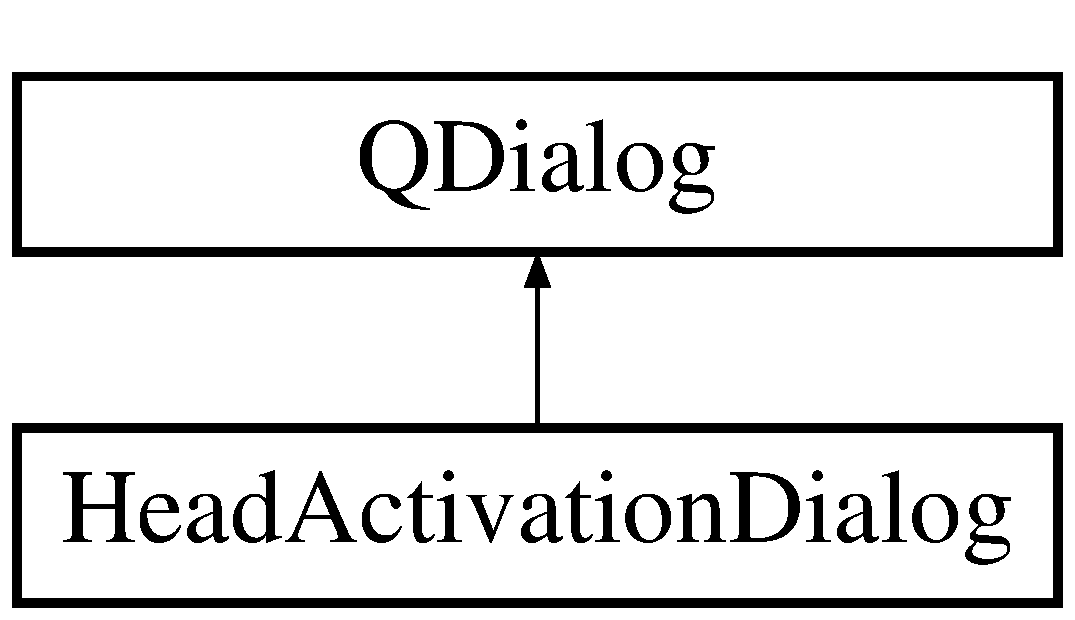
\includegraphics[height=2.000000cm]{classHeadActivationDialog}
\end{center}
\end{figure}
\subsubsection*{Signals}
\begin{DoxyCompactItemize}
\item 
void \mbox{\hyperlink{classHeadActivationDialog_ae76f8ea5faecab0d161904b14d925bda}{send\+Command}} (Q\+Byte\+Array cmd)
\end{DoxyCompactItemize}
\subsubsection*{Public Member Functions}
\begin{DoxyCompactItemize}
\item 
\mbox{\hyperlink{classHeadActivationDialog_aa8af7af33f3feac8547580e4c9bac577}{Head\+Activation\+Dialog}} (int \mbox{\hyperlink{classHeadActivationDialog_a0403b31877ebf58f738b9bfa68d31434}{head\+Count}}, Q\+Widget $\ast$parent=0)
\item 
\mbox{\hyperlink{classHeadActivationDialog_a277a05013a9304f1fc07ea89576e7b3d}{$\sim$\+Head\+Activation\+Dialog}} ()
\item 
void \mbox{\hyperlink{classHeadActivationDialog_a471339dee05798a94de85a2ee2cd43c4}{set\+Head\+Activ\+State}} (\mbox{\hyperlink{settings_8h_a4196118492a3b1493c81f250e90af775}{uint32\+\_\+t}} state)
\item 
\mbox{\hyperlink{settings_8h_a4196118492a3b1493c81f250e90af775}{uint32\+\_\+t}} \mbox{\hyperlink{classHeadActivationDialog_aa96f7a5383ade62d5bdf21fd2defac75}{get\+Head\+Activ\+State}} ()
\item 
bool \mbox{\hyperlink{classHeadActivationDialog_a1a6004ae7f92565dbf3bc42ff2f8cf5c}{get\+Head\+Activ\+At\+Index}} (int index)
\end{DoxyCompactItemize}
\subsubsection*{Protected Member Functions}
\begin{DoxyCompactItemize}
\item 
bool \mbox{\hyperlink{classHeadActivationDialog_aff7339cd3040bfcdc4e86d6e83a2e2da}{event}} (Q\+Event $\ast$e)
\item 
void \mbox{\hyperlink{classHeadActivationDialog_ae61da7b66bf8a351a83667e518455a5b}{show\+Event}} (Q\+Show\+Event $\ast$ev)
\item 
void \mbox{\hyperlink{classHeadActivationDialog_a7ffe0f22086377330bbea7117ff404e0}{change\+Event}} (Q\+Event $\ast$\mbox{\hyperlink{classHeadActivationDialog_aff7339cd3040bfcdc4e86d6e83a2e2da}{event}})
\end{DoxyCompactItemize}
\subsubsection*{Private Slots}
\begin{DoxyCompactItemize}
\item 
void \mbox{\hyperlink{classHeadActivationDialog_a544834488f3b17daa84f2f126cd405b1}{push\+Button\+O\+K\+\_\+clicked}} ()
\item 
void \mbox{\hyperlink{classHeadActivationDialog_af75039537fd16f02263e12343f7655c6}{push\+Button\+Cancel\+\_\+clicked}} ()
\item 
void \mbox{\hyperlink{classHeadActivationDialog_a2a6c18f85c6e70dcd242f29b14b44219}{head\+State\+Changed}} (int index)
\end{DoxyCompactItemize}
\subsubsection*{Private Attributes}
\begin{DoxyCompactItemize}
\item 
Ui\+::\+Head\+Activation\+Dialog $\ast$ \mbox{\hyperlink{classHeadActivationDialog_a2099e5d65b57cda6318d5d88b06157f6}{ui}}
\item 
Q\+List$<$ \mbox{\hyperlink{classCheckBoxIndexed}{Check\+Box\+Indexed}} $\ast$ $>$ \mbox{\hyperlink{classHeadActivationDialog_ae6fb828d26fda5b86510b5e427f24d06}{check\+Box\+List}}
\item 
int \mbox{\hyperlink{classHeadActivationDialog_a0403b31877ebf58f738b9bfa68d31434}{head\+Count}}
\item 
\mbox{\hyperlink{settings_8h_a4196118492a3b1493c81f250e90af775}{uint32\+\_\+t}} \mbox{\hyperlink{classHeadActivationDialog_a720bae08173514106fd2bdfda9a8e902}{head\+Activ\+State}}
\item 
bool \mbox{\hyperlink{classHeadActivationDialog_ab86719bd4a08237cba25753be6f831e9}{need\+Send\+Reset}}
\end{DoxyCompactItemize}


\subsubsection{Constructor \& Destructor Documentation}
\mbox{\Hypertarget{classHeadActivationDialog_aa8af7af33f3feac8547580e4c9bac577}\label{classHeadActivationDialog_aa8af7af33f3feac8547580e4c9bac577}} 
\index{Head\+Activation\+Dialog@{Head\+Activation\+Dialog}!Head\+Activation\+Dialog@{Head\+Activation\+Dialog}}
\index{Head\+Activation\+Dialog@{Head\+Activation\+Dialog}!Head\+Activation\+Dialog@{Head\+Activation\+Dialog}}
\paragraph{\texorpdfstring{Head\+Activation\+Dialog()}{HeadActivationDialog()}}
{\footnotesize\ttfamily Head\+Activation\+Dialog\+::\+Head\+Activation\+Dialog (\begin{DoxyParamCaption}\item[{int}]{head\+Count,  }\item[{Q\+Widget $\ast$}]{parent = {\ttfamily 0} }\end{DoxyParamCaption}){\ttfamily [explicit]}} - class constructor. Used to create widget with \hyperlink{classHeadActivationDialog_a0403b31877ebf58f738b9bfa68d31434}{head\+Count} Q\+Check\+Box widgets to allow user activate (or deactivate) heads.

\mbox{\Hypertarget{classHeadActivationDialog_a277a05013a9304f1fc07ea89576e7b3d}\label{classHeadActivationDialog_a277a05013a9304f1fc07ea89576e7b3d}} 
\index{Head\+Activation\+Dialog@{Head\+Activation\+Dialog}!````~Head\+Activation\+Dialog@{$\sim$\+Head\+Activation\+Dialog}}
\index{````~Head\+Activation\+Dialog@{$\sim$\+Head\+Activation\+Dialog}!Head\+Activation\+Dialog@{Head\+Activation\+Dialog}}
\paragraph{\texorpdfstring{$\sim$\+Head\+Activation\+Dialog()}{~HeadActivationDialog()}}
{\footnotesize\ttfamily Head\+Activation\+Dialog\+::$\sim$\+Head\+Activation\+Dialog (\begin{DoxyParamCaption}{ }\end{DoxyParamCaption})} - standard class destructor.



\subsubsection{Member Function Documentation}
\mbox{\Hypertarget{classHeadActivationDialog_a7ffe0f22086377330bbea7117ff404e0}\label{classHeadActivationDialog_a7ffe0f22086377330bbea7117ff404e0}} 
\index{Head\+Activation\+Dialog@{Head\+Activation\+Dialog}!change\+Event@{change\+Event}}
\index{change\+Event@{change\+Event}!Head\+Activation\+Dialog@{Head\+Activation\+Dialog}}
{\footnotesize\ttfamily void Head\+Activation\+Dialog\+::\texorpdfstring{change\+Event()}{changeEvent} (\begin{DoxyParamCaption}\item[{Q\+Event $\ast$}]{event }\end{DoxyParamCaption}){\ttfamily [protected]}} - reimplementation of default event for Q\+Dialog to enable user interface translation. Function called automatically.

\mbox{\Hypertarget{classHeadActivationDialog_aff7339cd3040bfcdc4e86d6e83a2e2da}\label{classHeadActivationDialog_aff7339cd3040bfcdc4e86d6e83a2e2da}} 
\index{Head\+Activation\+Dialog@{Head\+Activation\+Dialog}!event@{event}}
\index{event@{event}!Head\+Activation\+Dialog@{Head\+Activation\+Dialog}}
{\footnotesize\ttfamily bool Head\+Activation\+Dialog\+::\texorpdfstring{event()}{event} (\begin{DoxyParamCaption}\item[{Q\+Event $\ast$}]{e }\end{DoxyParamCaption}){\ttfamily [protected]}}- reimplementation of standard function to handle QEvent::WindowDeactivate or QEvent::Leave for automatic invoke \hyperlink{classHeadActivationDialog_a544834488f3b17daa84f2f126cd405b1}{push\+Button\+O\+K\+\_\+clicked}(...) function on window deactivation.

\mbox{\Hypertarget{classHeadActivationDialog_a1a6004ae7f92565dbf3bc42ff2f8cf5c}\label{classHeadActivationDialog_a1a6004ae7f92565dbf3bc42ff2f8cf5c}} 
\index{Head\+Activation\+Dialog@{Head\+Activation\+Dialog}!get\+Head\+Activ\+At\+Index@{get\+Head\+Activ\+At\+Index}}
\index{get\+Head\+Activ\+At\+Index@{get\+Head\+Activ\+At\+Index}!Head\+Activation\+Dialog@{Head\+Activation\+Dialog}}
{\footnotesize\ttfamily bool Head\+Activation\+Dialog\+::\texorpdfstring{get\+Head\+Activ\+At\+Index()}{getHeadActivAtIndex} (\begin{DoxyParamCaption}\item[{int}]{index }\end{DoxyParamCaption})} - function to get state of head according to given index. Return \textit{bool} value: \textit{true} if head active and \textit{false} if it is not.

\mbox{\Hypertarget{classHeadActivationDialog_aa96f7a5383ade62d5bdf21fd2defac75}\label{classHeadActivationDialog_aa96f7a5383ade62d5bdf21fd2defac75}} 
\index{Head\+Activation\+Dialog@{Head\+Activation\+Dialog}!get\+Head\+Activ\+State@{get\+Head\+Activ\+State}}
\index{get\+Head\+Activ\+State@{get\+Head\+Activ\+State}!Head\+Activation\+Dialog@{Head\+Activation\+Dialog}}
{\footnotesize\ttfamily \mbox{\hyperlink{settings_8h_a4196118492a3b1493c81f250e90af775}{uint32\+\_\+t}} Head\+Activation\+Dialog\+::\texorpdfstring{get\+Head\+Activ\+State()}{getHeadActivState}(\begin{DoxyParamCaption}{ }\end{DoxyParamCaption})} - function return state of heads in 32-bit variable. Position of bit describe head number.

\mbox{\Hypertarget{classHeadActivationDialog_a2a6c18f85c6e70dcd242f29b14b44219}\label{classHeadActivationDialog_a2a6c18f85c6e70dcd242f29b14b44219}} 
\index{Head\+Activation\+Dialog@{Head\+Activation\+Dialog}!head\+State\+Changed@{head\+State\+Changed}}
\index{head\+State\+Changed@{head\+State\+Changed}!Head\+Activation\+Dialog@{Head\+Activation\+Dialog}}
{\footnotesize\ttfamily void Head\+Activation\+Dialog\+::\texorpdfstring{head\+State\+Changed}{headStateChanged} (\begin{DoxyParamCaption}\item[{int}]{index }\end{DoxyParamCaption}){\ttfamily [private]}, {\ttfamily [slot]}} - function which called by check\+Boxes on window (from \hyperlink{classHeadActivationDialog_ae6fb828d26fda5b86510b5e427f24d06}{check\+Box\+List}). Function update \hyperlink{classHeadActivationDialog_a720bae08173514106fd2bdfda9a8e902}{head\+Activ\+State} value and send command to activate (or deactivate) heads to master board with \hyperlink{classHeadActivationDialog_ae76f8ea5faecab0d161904b14d925bda}{send\+Command} (Q\+Byte\+Array cmd) signal. 

\mbox{\Hypertarget{classHeadActivationDialog_af75039537fd16f02263e12343f7655c6}\label{classHeadActivationDialog_af75039537fd16f02263e12343f7655c6}} 
\index{Head\+Activation\+Dialog@{Head\+Activation\+Dialog}!push\+Button\+Cancel\+\_\+clicked@{push\+Button\+Cancel\+\_\+clicked}}
\index{push\+Button\+Cancel\+\_\+clicked@{push\+Button\+Cancel\+\_\+clicked}!Head\+Activation\+Dialog@{Head\+Activation\+Dialog}}
{\footnotesize\ttfamily void Head\+Activation\+Dialog\+::\texorpdfstring{push\+Button\+Cancel\+\_\+clicked}{pushButtonCancel\_clicked} (\begin{DoxyParamCaption}{ }\end{DoxyParamCaption}){\ttfamily [private]}, {\ttfamily [slot]}} - function call by \textit{'Cancel'} button and used to hide window. Button, which call function, can be disabled if user must apply changes in settings.

\mbox{\Hypertarget{classHeadActivationDialog_a544834488f3b17daa84f2f126cd405b1}\label{classHeadActivationDialog_a544834488f3b17daa84f2f126cd405b1}} 
\index{Head\+Activation\+Dialog@{Head\+Activation\+Dialog}!push\+Button\+O\+K\+\_\+clicked@{push\+Button\+O\+K\+\_\+clicked}}
\index{push\+Button\+O\+K\+\_\+clicked@{push\+Button\+O\+K\+\_\+clicked}!Head\+Activation\+Dialog@{Head\+Activation\+Dialog}}
{\footnotesize\ttfamily void Head\+Activation\+Dialog\+::\texorpdfstring{push\+Button\+O\+K\+\_\+clicked}{pushButtonOK\_clicked} (\begin{DoxyParamCaption}{ }\end{DoxyParamCaption}){\ttfamily [private]}, {\ttfamily [slot]}} - function call by \textit{'OK'} button and used to gather data and hide window.

\mbox{\Hypertarget{classHeadActivationDialog_ae76f8ea5faecab0d161904b14d925bda}\label{classHeadActivationDialog_ae76f8ea5faecab0d161904b14d925bda}} 
\index{Head\+Activation\+Dialog@{Head\+Activation\+Dialog}!send\+Command@{send\+Command}}
\index{send\+Command@{send\+Command}!Head\+Activation\+Dialog@{Head\+Activation\+Dialog}}
{\footnotesize\ttfamily void Head\+Activation\+Dialog\+::\texorpdfstring{send\+Command}{sendCommand} (\begin{DoxyParamCaption}\item[{Q\+Byte\+Array}]{cmd }\end{DoxyParamCaption}){\ttfamily [signal]}} - signal to send data in \textit{Q\+Byte\+Array} format to handle in parent object and send it to serial port.

\mbox{\Hypertarget{classHeadActivationDialog_a471339dee05798a94de85a2ee2cd43c4}\label{classHeadActivationDialog_a471339dee05798a94de85a2ee2cd43c4}} 
\index{Head\+Activation\+Dialog@{Head\+Activation\+Dialog}!set\+Head\+Activ\+State@{set\+Head\+Activ\+State}}
\index{set\+Head\+Activ\+State@{set\+Head\+Activ\+State}!Head\+Activation\+Dialog@{Head\+Activation\+Dialog}}
{\footnotesize\ttfamily void Head\+Activation\+Dialog\+::\texorpdfstring{set\+Head\+Activ\+State()}{setHeadActivState()} (\begin{DoxyParamCaption}\item[{\mbox{\hyperlink{settings_8h_a4196118492a3b1493c81f250e90af775}{uint32\+\_\+t}}}]{state }\end{DoxyParamCaption})} - function to set \hyperlink{classHeadActivationDialog_a720bae08173514106fd2bdfda9a8e902}{head\+Activ\+State} value and set check\+Boxes on window (from \hyperlink{classHeadActivationDialog_ae6fb828d26fda5b86510b5e427f24d06}{check\+Box\+List}) to appropriate state.

\mbox{\Hypertarget{classHeadActivationDialog_ae61da7b66bf8a351a83667e518455a5b}\label{classHeadActivationDialog_ae61da7b66bf8a351a83667e518455a5b}} 
\index{Head\+Activation\+Dialog@{Head\+Activation\+Dialog}!show\+Event@{show\+Event}}
\index{show\+Event@{show\+Event}!Head\+Activation\+Dialog@{Head\+Activation\+Dialog}}
{\footnotesize\ttfamily void Head\+Activation\+Dialog\+::\texorpdfstring{show\+Event()}{showEvent} (\begin{DoxyParamCaption}\item[{Q\+Show\+Event $\ast$}]{ev }\end{DoxyParamCaption}){\ttfamily [protected]}} - reimplementation of standard event handler; used for update state of \hyperlink{classHeadActivationDialog_ae6fb828d26fda5b86510b5e427f24d06}{check\+Box\+List} items.



\subsubsection{Member Data Documentation}
\mbox{\Hypertarget{classHeadActivationDialog_ae6fb828d26fda5b86510b5e427f24d06}\label{classHeadActivationDialog_ae6fb828d26fda5b86510b5e427f24d06}} 
\index{Head\+Activation\+Dialog@{Head\+Activation\+Dialog}!check\+Box\+List@{check\+Box\+List}}
\index{check\+Box\+List@{check\+Box\+List}!Head\+Activation\+Dialog@{Head\+Activation\+Dialog}}
{\footnotesize\ttfamily Q\+List$<$\mbox{\hyperlink{classCheckBoxIndexed}{Check\+Box\+Indexed}}$\ast$$>$ Head\+Activation\+Dialog\+::\texorpdfstring{check\+Box\+List}{checkBoxList}{\ttfamily [private]}} - list of redefined Q\+Check\+Box class objects. All list items are showed on dialog and used to activate (or deactivate) heads. 

\mbox{\Hypertarget{classHeadActivationDialog_a720bae08173514106fd2bdfda9a8e902}\label{classHeadActivationDialog_a720bae08173514106fd2bdfda9a8e902}} 
\index{Head\+Activation\+Dialog@{Head\+Activation\+Dialog}!head\+Activ\+State@{head\+Activ\+State}}
\index{head\+Activ\+State@{head\+Activ\+State}!Head\+Activation\+Dialog@{Head\+Activation\+Dialog}}
{\footnotesize\ttfamily \mbox{\hyperlink{settings_8h_a4196118492a3b1493c81f250e90af775}{uint32\+\_\+t}} Head\+Activation\+Dialog\+::\texorpdfstring{head\+Activ\+State}{headActivState}{\ttfamily [private]}}

\mbox{\Hypertarget{classHeadActivationDialog_a0403b31877ebf58f738b9bfa68d31434}\label{classHeadActivationDialog_a0403b31877ebf58f738b9bfa68d31434}} 
\index{Head\+Activation\+Dialog@{Head\+Activation\+Dialog}!head\+Count@{head\+Count}}
\index{head\+Count@{head\+Count}!Head\+Activation\+Dialog@{Head\+Activation\+Dialog}}
{\footnotesize\ttfamily int Head\+Activation\+Dialog\+::\texorpdfstring{head\+Count}{headCount}{\ttfamily [private]}}

\mbox{\Hypertarget{classHeadActivationDialog_ab86719bd4a08237cba25753be6f831e9}\label{classHeadActivationDialog_ab86719bd4a08237cba25753be6f831e9}} 
\index{Head\+Activation\+Dialog@{Head\+Activation\+Dialog}!need\+Send\+Reset@{need\+Send\+Reset}}
\index{need\+Send\+Reset@{need\+Send\+Reset}!Head\+Activation\+Dialog@{Head\+Activation\+Dialog}}
{\footnotesize\ttfamily bool Head\+Activation\+Dialog\+::\texorpdfstring{need\+Send\+Reset}{needSendReset}{\ttfamily [private]}}

The documentation for this class was generated from the following files\+:\begin{DoxyCompactItemize}
\item 
\mbox{\hyperlink{headactivationdialog_8h}{headactivationdialog.\+h}}\item 
\mbox{\hyperlink{headactivationdialog_8cpp}{headactivationdialog.\+cpp}}\end{DoxyCompactItemize}
\newpage
\hypertarget{structHeadSetting_1_1HeadComands__}{}\subsection{Head\+Setting\+:\+:Head\+Comands\+\_\+ Struct Reference}
\label{structHeadSetting_1_1HeadComands__}\index{Head\+Setting\+::\+Head\+Comands\+\_\+@{Head\+Setting\+::\+Head\+Comands\+\_\+}}


{\ttfamily \#include $<$settings.\+h$>$}

\subsubsection*{Public Attributes}
\begin{DoxyCompactItemize}
\item 
\mbox{\hyperlink{classHeadSetting_afe9523cb7fbbae2db026b1fca4a02be3}{Head\+Commands\+En}} \mbox{\hyperlink{structHeadSetting_1_1HeadComands___a7811619ec45cfc46a55b679f43e3aac3}{head\+Cmd}}
\end{DoxyCompactItemize}


\subsubsection{Member Data Documentation}
\mbox{\Hypertarget{structHeadSetting_1_1HeadComands___a7811619ec45cfc46a55b679f43e3aac3}\label{structHeadSetting_1_1HeadComands___a7811619ec45cfc46a55b679f43e3aac3}} 
\index{Head\+Setting\+::\+Head\+Comands\+\_\+@{Head\+Setting\+::\+Head\+Comands\+\_\+}!head\+Cmd@{head\+Cmd}}
\index{head\+Cmd@{head\+Cmd}!Head\+Setting\+::\+Head\+Comands\+\_\+@{Head\+Setting\+::\+Head\+Comands\+\_\+}}
{\footnotesize\ttfamily \mbox{\hyperlink{classHeadSetting_afe9523cb7fbbae2db026b1fca4a02be3}{Head\+Commands\+En}} Head\+Setting\+::\+Head\+Comands\+\_\+\+::\texorpdfstring{head\+Cmd}{headCmd}} - enumerator of commands which are send to head PCB's 



The documentation for this struct was generated from the following file\+:\begin{DoxyCompactItemize}
\item 
\mbox{\hyperlink{settings_8h}{settings.\+h}}\end{DoxyCompactItemize}
\newpage
\hypertarget{classHeadForm}{}\subsection{Head\+Form Class Reference}
\label{classHeadForm}\index{Head\+Form@{Head\+Form}}


{\ttfamily \#include $<$headform.\+h$>$}

Inheritance diagram for Head\+Form\+:\begin{figure}[H]
\begin{center}
\leavevmode
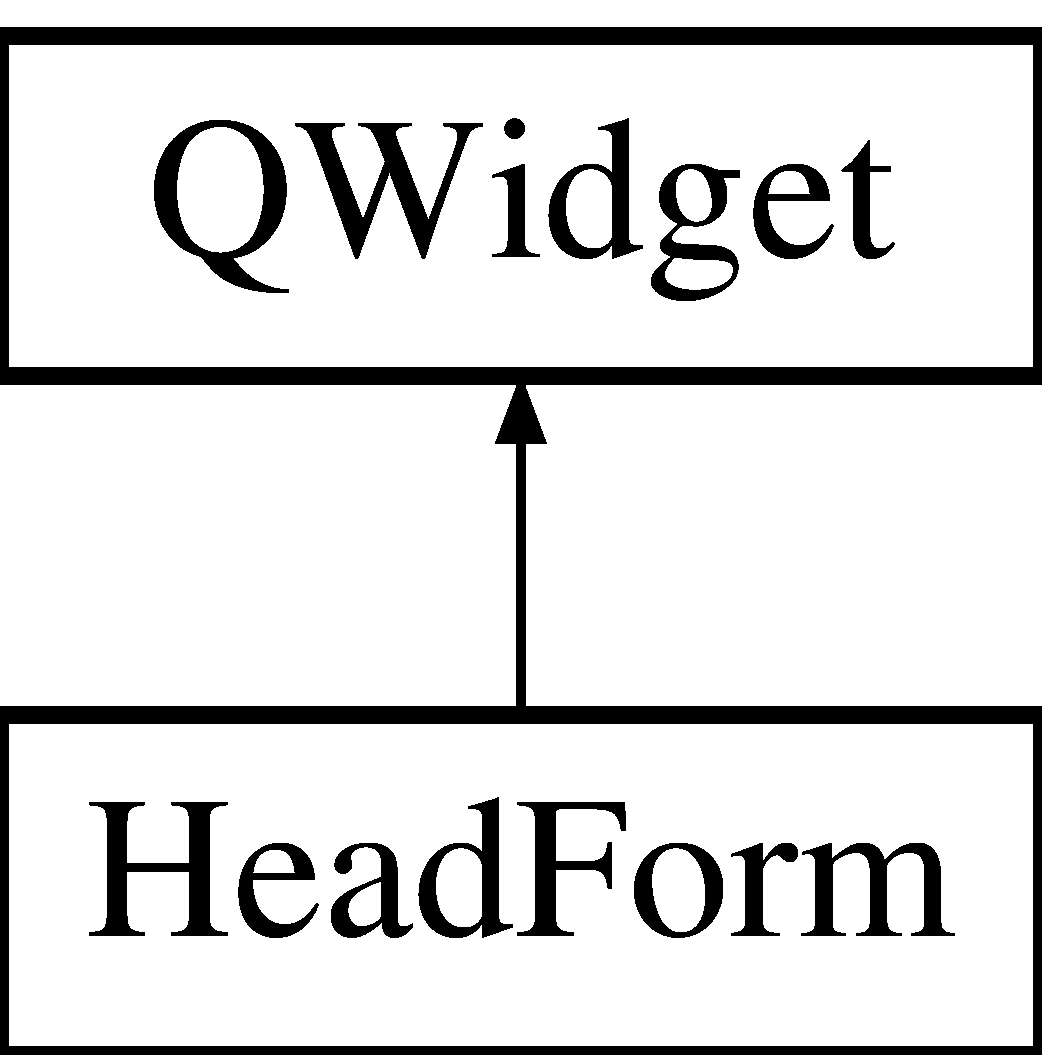
\includegraphics[height=2.000000cm]{classHeadForm}
\end{center}
\end{figure}
\subsubsection*{Public Types}
\begin{DoxyCompactItemize}
\item 
enum \mbox{\hyperlink{classHeadForm_ae17d4f6887245f37b3f7c002dd226dd0}{Headform\+Type\+\_\+}} \{ \mbox{\hyperlink{classHeadForm_ae17d4f6887245f37b3f7c002dd226dd0a4652ee386f0507081c73c94e23406355}{Head\+Puting\+On}}, 
\mbox{\hyperlink{classHeadForm_ae17d4f6887245f37b3f7c002dd226dd0ae0daafb321b4253abd5c15a5bee4073d}{Head\+Removing}}, 
\mbox{\hyperlink{classHeadForm_ae17d4f6887245f37b3f7c002dd226dd0a1aa31669b6be4f549f4635ab9bedf87c}{Head\+Processing}}
 \}
\item 
enum \mbox{\hyperlink{classHeadForm_ad43012a40fdd353f422cc70c37dd61f8}{Headform\+State\+\_\+}} \{ \mbox{\hyperlink{classHeadForm_ad43012a40fdd353f422cc70c37dd61f8ab400a883c6b3712cb04d90d43fc90574}{shirt\+On}}, 
\mbox{\hyperlink{classHeadForm_ad43012a40fdd353f422cc70c37dd61f8a4602d887a83fe4055d613fbe3ecb9dbc}{shirt\+Off}}, 
\mbox{\hyperlink{classHeadForm_ad43012a40fdd353f422cc70c37dd61f8af061092a97b564b96638af440f6c8e3c}{shirt\+Processing}}
 \}
\item 
enum \mbox{\hyperlink{classHeadForm_a26cd2569dd333f30e239f5ce00a267c5}{Sett\+Btn\+Pos\+\_\+}} \{ \mbox{\hyperlink{classHeadForm_a26cd2569dd333f30e239f5ce00a267c5a8964ad65c812d4a1fdd515a043281dc8}{At\+Left\+Up}}, 
\mbox{\hyperlink{classHeadForm_a26cd2569dd333f30e239f5ce00a267c5ac8f51999e1bc4dc81f2a5362246ab8cb}{At\+Left\+Down}}, 
\mbox{\hyperlink{classHeadForm_a26cd2569dd333f30e239f5ce00a267c5a50f633b215328280784cf90a9d66bf6f}{At\+Right\+Up}}, 
\mbox{\hyperlink{classHeadForm_a26cd2569dd333f30e239f5ce00a267c5ade80fd3660fc8764b6fc9a9d311b3d47}{At\+Right\+Down}}
 \}
\item typedef enum \mbox{\hyperlink{classHeadForm_ae17d4f6887245f37b3f7c002dd226dd0}{Head\+Form\+::\+Headform\+Type\+\_\+}} \mbox{\hyperlink{classHeadForm_a15bfe98cd74c9677947211a02313f7d1}{Headform\+Type}}
\item 
typedef enum \mbox{\hyperlink{classHeadForm_ad43012a40fdd353f422cc70c37dd61f8}{Head\+Form\+::\+Headform\+State\+\_\+}} \mbox{\hyperlink{classHeadForm_ae7f8ba0c9db5a5140ac4e3417dc1d9b2}{Headform\+State}}
\item 
typedef enum \mbox{\hyperlink{classHeadForm_a26cd2569dd333f30e239f5ce00a267c5}{Head\+Form\+::\+Sett\+Btn\+Pos\+\_\+}} \mbox{\hyperlink{classHeadForm_ae0ae43de172739d43f503ff0a03aad1a}{Sett\+Btn\+Pos}}
\end{DoxyCompactItemize}
\subsubsection*{Signals}
\begin{DoxyCompactItemize}
\item 
void \mbox{\hyperlink{classHeadForm_ad5033138e38409217e1ae343c71afc64}{setting\+Button\+Cliced}} (int \mbox{\hyperlink{classHeadForm_a5e01a73f3b47bdc85ea85f5650cdf0d0}{index}})
\item 
void \mbox{\hyperlink{classHeadForm_a6e4fb0f70f7571685094e53836bcbe21}{load\+State\+Changed}} (int \mbox{\hyperlink{classHeadForm_a5e01a73f3b47bdc85ea85f5650cdf0d0}{index}}, \mbox{\hyperlink{headform_8h_a56d194976643934b3332b3f99d82490d}{Load\+State}} state)
\end{DoxyCompactItemize}
\subsubsection*{Public Member Functions}
\begin{DoxyCompactItemize}
\item 
\mbox{\hyperlink{classHeadForm_a9474e3d5af0aad57f847d1a38eba8591}{Head\+Form}} (Q\+Widget $\ast$parent=0)
\item 
\mbox{\hyperlink{classHeadForm_ac4a0350cd62ed18740505fe61ba75d80}{$\sim$\+Head\+Form}} ()
\item 
void \mbox{\hyperlink{classHeadForm_acd6d67e3691918b0e4c6716b079e67d0}{set\+Index}} (int i)
\item 
void \mbox{\hyperlink{classHeadForm_af74e0d29b259aa4f2e9529346237207a}{set\+Index\+Label\+Position}} (\mbox{\hyperlink{classHeadForm_ae0ae43de172739d43f503ff0a03aad1a}{Sett\+Btn\+Pos}} position)
\item 
void \mbox{\hyperlink{classHeadForm_ac2845f30dc7686178380c9c108b4c5bf}{set\+Pixmap}} (\mbox{\hyperlink{classHeadForm_ae7f8ba0c9db5a5140ac4e3417dc1d9b2}{Headform\+State}} state, Q\+String st\+Str)
\item 
void \mbox{\hyperlink{classHeadForm_a934e12ca808cb22f74734df9852e7146}{set\+Pixmap}} (\mbox{\hyperlink{classHeadForm_ae7f8ba0c9db5a5140ac4e3417dc1d9b2}{Headform\+State}} state)
\item 
void \mbox{\hyperlink{classHeadForm_aaa15b61ff5f3bdbf8c3e7a329fb6b0cb}{set\+Rag\+On}} (bool state)
\item 
void \mbox{\hyperlink{classHeadForm_acb2b064f0453aeed4a5bea49cc33be47}{set\+Icon\+Path}} (Q\+String path)
\item 
void \mbox{\hyperlink{classHeadForm_a69a9f3ad37ba31a3c1f8a5c491b6272d}{set\+Rag\+Color}} (Q\+Color color)
\item 
void \mbox{\hyperlink{classHeadForm_a8e86ad0f2d29ec594c62dbfd253b5fee}{set\+Strok\+Count}} (int val)
\item 
void \mbox{\hyperlink{classHeadForm_a6b5082ea42b171300a105d6a35d52c91}{set\+Step\+Bk\+Str\+Cnt}} (int val)
\item 
void \mbox{\hyperlink{classHeadForm_afd37ba9a460ed5bf74c5b0b40394feb5}{set\+Dry\+Power}} (int val)
\item 
void \mbox{\hyperlink{classHeadForm_a75d114050b779cd5793a4968b06e8178}{set\+Off}} ()
\item 
\mbox{\hyperlink{classHeadForm_ae7f8ba0c9db5a5140ac4e3417dc1d9b2}{Headform\+State}} \mbox{\hyperlink{classHeadForm_a35de102780fe0011543c31d62f8bd72e}{get\+Rag\+State}} ()
\item 
void \mbox{\hyperlink{classHeadForm_aa61be1b4d88c7afbfff172190d40cc07}{set\+Headform\+Type}} (\mbox{\hyperlink{classHeadForm_a15bfe98cd74c9677947211a02313f7d1}{Headform\+Type}} type)
\item 
\mbox{\hyperlink{classHeadForm_a15bfe98cd74c9677947211a02313f7d1}{Headform\+Type}} \mbox{\hyperlink{classHeadForm_a8e521c0edb67751bebcc8f82e9176a16}{get\+Headform\+Type}} ()
\item 
Q\+Size \mbox{\hyperlink{classHeadForm_a138f7ab8bf3996a036e587b0ea7f4237}{get\+Label\+Size}} ()
\end{DoxyCompactItemize}
\subsubsection*{Protected Member Functions}
\begin{DoxyCompactItemize}
\item 
void \mbox{\hyperlink{classHeadForm_a922c24b7eb4d084712d0ec4e9a084e90}{mouse\+Press\+Event}} (Q\+Mouse\+Event $\ast$event)
\end{DoxyCompactItemize}
\subsubsection*{Private Attributes}
\begin{DoxyCompactItemize}
\item 
Ui\+::\+Head\+Form $\ast$ \mbox{\hyperlink{classHeadForm_afd952edd2f6b6e9ccd02f18ddf694ad1}{ui}}
\item 
Q\+Label $\ast$ \mbox{\hyperlink{classHeadForm_adbc068754f789e1a63c113f1ce7caf38}{label\+Index}}
\item 
Q\+Label $\ast$ \mbox{\hyperlink{classHeadForm_a591efe6e830fd170cb549bca142d2759}{label\+Strok\+Cnt}}
\item 
Q\+Label $\ast$ \mbox{\hyperlink{classHeadForm_a1a7f706cff05b5644d3eae9ab21b2caf}{label\+St\+Bk\+Str}}
\item 
Q\+Image \mbox{\hyperlink{classHeadForm_a30f30561d242211ed827ffaf627e0839}{pix\+Shirt\+Show}}
\item 
Q\+Image \mbox{\hyperlink{classHeadForm_a54d7609f912aa7b0edd6850e1f57f0a0}{pix\+Shirt\+Hide}}
\item 
Q\+Image \mbox{\hyperlink{classHeadForm_aa44a452750fe6db786814ec502f0d655}{pix\+Shirt\+Animate}}
\item 
Q\+Graphics\+Colorize\+Effect $\ast$ \mbox{\hyperlink{classHeadForm_a65805e9d52c18a00fd2bece0f560f26a}{graph\+Effect}}
\item 
Q\+String \mbox{\hyperlink{classHeadForm_a88124373bcbdb5679ea11608362e485b}{path\+Image}}
\item 
int \mbox{\hyperlink{classHeadForm_a5e01a73f3b47bdc85ea85f5650cdf0d0}{index}}
\item 
\mbox{\hyperlink{classHeadForm_ae7f8ba0c9db5a5140ac4e3417dc1d9b2}{Headform\+State}} \mbox{\hyperlink{classHeadForm_a0ffd2cf8eea50202d72c4bf286a11916}{headform\+State}}
\item 
\mbox{\hyperlink{classHeadForm_a15bfe98cd74c9677947211a02313f7d1}{Headform\+Type}} \mbox{\hyperlink{classHeadForm_a5f448e8b1081f12332f699d029fa8433}{headform\+Type}}
\item 
Q\+Graphics\+Scene $\ast$ \mbox{\hyperlink{classHeadForm_ac4615e0489c20f6753a1804bfb9d188a}{gr\+Scene}}
\item 
Q\+Graphics\+Pixmap\+Item $\ast$ \mbox{\hyperlink{classHeadForm_a974e25ac4edb0f0a25da108c0b4da4a1}{gr\+Pix\+Logo\+Item}}
\item 
Q\+Graphics\+Rect\+Item $\ast$ \mbox{\hyperlink{classHeadForm_acc0cb81dc7cb95b72af6f44ebcc90f4e}{gr\+Rect\+Bkgr\+Item}}
\item 
Q\+Rect \mbox{\hyperlink{classHeadForm_a472b95713a709b727b84af2572f0f4f6}{gr\+Size}}
\item 
\mbox{\hyperlink{classHeadForm_ae0ae43de172739d43f503ff0a03aad1a}{Head\+Form\+::\+Sett\+Btn\+Pos}} \mbox{\hyperlink{classHeadForm_a3f9306937e89ae7a306034c875efc48e}{label\+Pos}}
\end{DoxyCompactItemize}


\subsubsection{Member Typedef Documentation}
\mbox{\Hypertarget{classHeadForm_ae7f8ba0c9db5a5140ac4e3417dc1d9b2}\label{classHeadForm_ae7f8ba0c9db5a5140ac4e3417dc1d9b2}} 
\index{Head\+Form@{Head\+Form}!Headform\+State@{Headform\+State}}
\index{Headform\+State@{Headform\+State}!Head\+Form@{Head\+Form}}
{\footnotesize\ttfamily typedef enum \mbox{\hyperlink{classHeadForm_ad43012a40fdd353f422cc70c37dd61f8}{Head\+Form\+::\+Headform\+State\+\_\+}} \mbox{\hyperlink{classHeadForm_ae7f8ba0c9db5a5140ac4e3417dc1d9b2}{Head\+Form\+::\+\texorpdfstring{Headform\+State}{HeadformState}}}}

\mbox{\Hypertarget{classHeadForm_a15bfe98cd74c9677947211a02313f7d1}\label{classHeadForm_a15bfe98cd74c9677947211a02313f7d1}} 
\index{Head\+Form@{Head\+Form}!Headform\+Type@{Headform\+Type}}
\index{Headform\+Type@{Headform\+Type}!Head\+Form@{Head\+Form}}
{\footnotesize\ttfamily typedef enum \mbox{\hyperlink{classHeadForm_ae17d4f6887245f37b3f7c002dd226dd0}{Head\+Form\+::\+Headform\+Type\+\_\+}} \mbox{\hyperlink{classHeadForm_a15bfe98cd74c9677947211a02313f7d1}{Head\+Form\+::\+\texorpdfstring{Headform\+Type}{HeadformType}}}}

\mbox{\Hypertarget{classHeadForm_ae0ae43de172739d43f503ff0a03aad1a}\label{classHeadForm_ae0ae43de172739d43f503ff0a03aad1a}} 
\index{Head\+Form@{Head\+Form}!Sett\+Btn\+Pos@{Sett\+Btn\+Pos}}
\index{Sett\+Btn\+Pos@{Sett\+Btn\+Pos}!Head\+Form@{Head\+Form}}
{\footnotesize\ttfamily typedef enum \mbox{\hyperlink{classHeadForm_a26cd2569dd333f30e239f5ce00a267c5}{Head\+Form\+::\+Sett\+Btn\+Pos\+\_\+}} \mbox{\hyperlink{classHeadForm_ae0ae43de172739d43f503ff0a03aad1a}{Head\+Form\+::\+\texorpdfstring{Sett\+Btn\+Pos}{SettBtnPos}}}}

\subsubsection{Member Enumeration Documentation}
\mbox{\Hypertarget{classHeadForm_ad43012a40fdd353f422cc70c37dd61f8}\label{classHeadForm_ad43012a40fdd353f422cc70c37dd61f8}} 
\index{Head\+Form@{Head\+Form}!Headform\+State\+\_\+@{Headform\+State\+\_\+}}
\index{Headform\+State\+\_\+@{Headform\+State\+\_\+}!Head\+Form@{Head\+Form}}
{\footnotesize\ttfamily enum \mbox{\hyperlink{classHeadForm_ad43012a40fdd353f422cc70c37dd61f8}{Head\+Form\+::\texorpdfstring{Headform\+State\+\_\+}{HeadformState\_}}}}

\begin{DoxyEnumFields}{Enumerator}
\raisebox{\heightof{T}}[0pt][0pt]{\index{shirt\+On@{shirt\+On}!Head\+Form@{Head\+Form}}\index{Head\+Form@{Head\+Form}!shirt\+On@{shirt\+On}}}\mbox{\Hypertarget{classHeadForm_ad43012a40fdd353f422cc70c37dd61f8ab400a883c6b3712cb04d90d43fc90574}\label{classHeadForm_ad43012a40fdd353f422cc70c37dd61f8ab400a883c6b3712cb04d90d43fc90574}} 
shirt\+On&show rag image on form.\\
\hline

\raisebox{\heightof{T}}[0pt][0pt]{\index{shirt\+Off@{shirt\+Off}!Head\+Form@{Head\+Form}}\index{Head\+Form@{Head\+Form}!shirt\+Off@{shirt\+Off}}}\mbox{\Hypertarget{classHeadForm_ad43012a40fdd353f422cc70c37dd61f8a4602d887a83fe4055d613fbe3ecb9dbc}\label{classHeadForm_ad43012a40fdd353f422cc70c37dd61f8a4602d887a83fe4055d613fbe3ecb9dbc}} 
shirt\+Off&hide rag image on form.\\
\hline

\raisebox{\heightof{T}}[0pt][0pt]{\index{shirt\+Processing@{shirt\+Processing}!Head\+Form@{Head\+Form}}\index{Head\+Form@{Head\+Form}!shirt\+Processing@{shirt\+Processing}}}\mbox{\Hypertarget{classHeadForm_ad43012a40fdd353f422cc70c37dd61f8af061092a97b564b96638af440f6c8e3c}\label{classHeadForm_ad43012a40fdd353f422cc70c37dd61f8af061092a97b564b96638af440f6c8e3c}} 
shirt\+Processing&show rag image animation on form.\\
\hline

\end{DoxyEnumFields}
\mbox{\Hypertarget{classHeadForm_ae17d4f6887245f37b3f7c002dd226dd0}\label{classHeadForm_ae17d4f6887245f37b3f7c002dd226dd0}} 
\index{Head\+Form@{Head\+Form}!Headform\+Type\+\_\+@{Headform\+Type\+\_\+}}
\index{Headform\+Type\+\_\+@{Headform\+Type\+\_\+}!Head\+Form@{Head\+Form}}
{\footnotesize\ttfamily enum \mbox{\hyperlink{classHeadForm_ae17d4f6887245f37b3f7c002dd226dd0}{Head\+Form\+::\+\texorpdfstring{Headform\+Type\+\_\+}{HeadformType\_}}}}

\begin{DoxyEnumFields}{Enumerator}
\raisebox{\heightof{T}}[0pt][0pt]{\index{Head\+Puting\+On@{Head\+Puting\+On}!Head\+Form@{Head\+Form}}\index{Head\+Form@{Head\+Form}!Head\+Puting\+On@{Head\+Puting\+On}}}\mbox{\Hypertarget{classHeadForm_ae17d4f6887245f37b3f7c002dd226dd0a4652ee386f0507081c73c94e23406355}\label{classHeadForm_ae17d4f6887245f37b3f7c002dd226dd0a4652ee386f0507081c73c94e23406355}} 
Head\+Puting\+On&paint load pallet to appropriate color.\\
\hline

\raisebox{\heightof{T}}[0pt][0pt]{\index{Head\+Removing@{Head\+Removing}!Head\+Form@{Head\+Form}}\index{Head\+Form@{Head\+Form}!Head\+Removing@{Head\+Removing}}}\mbox{\Hypertarget{classHeadForm_ae17d4f6887245f37b3f7c002dd226dd0ae0daafb321b4253abd5c15a5bee4073d}\label{classHeadForm_ae17d4f6887245f37b3f7c002dd226dd0ae0daafb321b4253abd5c15a5bee4073d}} 
Head\+Removing&paint unload pallet to appropriate color.\\
\hline

\raisebox{\heightof{T}}[0pt][0pt]{\index{Head\+Processing@{Head\+Processing}!Head\+Form@{Head\+Form}}\index{Head\+Form@{Head\+Form}!Head\+Processing@{Head\+Processing}}}\mbox{\Hypertarget{classHeadForm_ae17d4f6887245f37b3f7c002dd226dd0a1aa31669b6be4f549f4635ab9bedf87c}\label{classHeadForm_ae17d4f6887245f37b3f7c002dd226dd0a1aa31669b6be4f549f4635ab9bedf87c}} 
Head\+Processing&paint processing pallet to appropriate color.\\
\hline

\end{DoxyEnumFields}
\mbox{\Hypertarget{classHeadForm_a26cd2569dd333f30e239f5ce00a267c5}\label{classHeadForm_a26cd2569dd333f30e239f5ce00a267c5}} 
\index{Head\+Form@{Head\+Form}!Sett\+Btn\+Pos\+\_\+@{Sett\+Btn\+Pos\+\_\+}}
\index{Sett\+Btn\+Pos\+\_\+@{Sett\+Btn\+Pos\+\_\+}!Head\+Form@{Head\+Form}}
{\footnotesize\ttfamily enum \mbox{\hyperlink{classHeadForm_a26cd2569dd333f30e239f5ce00a267c5}{Head\+Form\+::\texorpdfstring{Sett\+Btn\+Pos\+\_\+}{SettBtnPos\_}}}} - describe position of \hyperlink{classHeadForm_adbc068754f789e1a63c113f1ce7caf38}{label\+Index}, \hyperlink{classHeadForm_a591efe6e830fd170cb549bca142d2759}{label\+Strok\+Cnt} and \hyperlink{classHeadForm_a1a7f706cff05b5644d3eae9ab21b2caf}{label\+St\+Bk\+Str}

\begin{DoxyEnumFields}{Enumerator}
\raisebox{\heightof{T}}[0pt][0pt]{\index{At\+Left\+Up@{At\+Left\+Up}!Head\+Form@{Head\+Form}}\index{Head\+Form@{Head\+Form}!At\+Left\+Up@{At\+Left\+Up}}}\mbox{\Hypertarget{classHeadForm_a26cd2569dd333f30e239f5ce00a267c5a8964ad65c812d4a1fdd515a043281dc8}\label{classHeadForm_a26cd2569dd333f30e239f5ce00a267c5a8964ad65c812d4a1fdd515a043281dc8}} 
At\+Left\+Up&\\
\hline

\raisebox{\heightof{T}}[0pt][0pt]{\index{At\+Left\+Down@{At\+Left\+Down}!Head\+Form@{Head\+Form}}\index{Head\+Form@{Head\+Form}!At\+Left\+Down@{At\+Left\+Down}}}\mbox{\Hypertarget{classHeadForm_a26cd2569dd333f30e239f5ce00a267c5ac8f51999e1bc4dc81f2a5362246ab8cb}\label{classHeadForm_a26cd2569dd333f30e239f5ce00a267c5ac8f51999e1bc4dc81f2a5362246ab8cb}} 
At\+Left\+Down&\\
\hline

\raisebox{\heightof{T}}[0pt][0pt]{\index{At\+Right\+Up@{At\+Right\+Up}!Head\+Form@{Head\+Form}}\index{Head\+Form@{Head\+Form}!At\+Right\+Up@{At\+Right\+Up}}}\mbox{\Hypertarget{classHeadForm_a26cd2569dd333f30e239f5ce00a267c5a50f633b215328280784cf90a9d66bf6f}\label{classHeadForm_a26cd2569dd333f30e239f5ce00a267c5a50f633b215328280784cf90a9d66bf6f}} 
At\+Right\+Up&\\
\hline

\raisebox{\heightof{T}}[0pt][0pt]{\index{At\+Right\+Down@{At\+Right\+Down}!Head\+Form@{Head\+Form}}\index{Head\+Form@{Head\+Form}!At\+Right\+Down@{At\+Right\+Down}}}\mbox{\Hypertarget{classHeadForm_a26cd2569dd333f30e239f5ce00a267c5ade80fd3660fc8764b6fc9a9d311b3d47}\label{classHeadForm_a26cd2569dd333f30e239f5ce00a267c5ade80fd3660fc8764b6fc9a9d311b3d47}} 
At\+Right\+Down&\\
\hline

\end{DoxyEnumFields}


\subsubsection{Constructor \& Destructor Documentation}
\mbox{\Hypertarget{classHeadForm_a9474e3d5af0aad57f847d1a38eba8591}\label{classHeadForm_a9474e3d5af0aad57f847d1a38eba8591}} 
\index{Head\+Form@{Head\+Form}!Head\+Form@{Head\+Form}}
\index{Head\+Form@{Head\+Form}!Head\+Form@{Head\+Form}}
\paragraph{\texorpdfstring{Head\+Form()}{HeadForm()}}
{\footnotesize\ttfamily Head\+Form\+::\+Head\+Form (\begin{DoxyParamCaption}\item[{Q\+Widget $\ast$}]{parent = {\ttfamily 0} }\end{DoxyParamCaption})} - constructor of class. Create Q\+Widget class object, initialize Q\+Label 's, Q\+Graphic\+Scene etc.

\mbox{\Hypertarget{classHeadForm_ac4a0350cd62ed18740505fe61ba75d80}\label{classHeadForm_ac4a0350cd62ed18740505fe61ba75d80}} 
\index{Head\+Form@{Head\+Form}!````~Head\+Form@{$\sim$\+Head\+Form}}
\index{````~Head\+Form@{$\sim$\+Head\+Form}!Head\+Form@{Head\+Form}}
\paragraph{\texorpdfstring{$\sim$\+Head\+Form()}{~HeadForm()}}
{\footnotesize\ttfamily Head\+Form\+::$\sim$\+Head\+Form (\begin{DoxyParamCaption}{ }\end{DoxyParamCaption})} - standard class destructor.



\subsubsection{Member Function Documentation}
\mbox{\Hypertarget{classHeadForm_a8e521c0edb67751bebcc8f82e9176a16}\label{classHeadForm_a8e521c0edb67751bebcc8f82e9176a16}} 
\index{Head\+Form@{Head\+Form}!get\+Headform\+Type@{get\+Headform\+Type}}
\index{get\+Headform\+Type@{get\+Headform\+Type}!Head\+Form@{Head\+Form}}
{\footnotesize\ttfamily \mbox{\hyperlink{classHeadForm_a15bfe98cd74c9677947211a02313f7d1}{Head\+Form\+::\+Headform\+Type}} Head\+Form\+::\texorpdfstring{get\+Headform\+Type}{getHeadformType} (\begin{DoxyParamCaption}{ }\end{DoxyParamCaption})} - function to get head type. Return one of \hyperlink{classHeadForm_ae17d4f6887245f37b3f7c002dd226dd0}{Headform\+Type\+\_\+} values.

\mbox{\Hypertarget{classHeadForm_a138f7ab8bf3996a036e587b0ea7f4237}\label{classHeadForm_a138f7ab8bf3996a036e587b0ea7f4237}} 
\index{Head\+Form@{Head\+Form}!get\+Label\+Size@{get\+Label\+Size}}
\index{get\+Label\+Size@{get\+Label\+Size}!Head\+Form@{Head\+Form}}
{\footnotesize\ttfamily Q\+Size Head\+Form\+::\texorpdfstring{get\+Label\+Size}{getLabelSize} (\begin{DoxyParamCaption}{ }\end{DoxyParamCaption})} - return size of Q\+Graphic\+View object in pixels.

\mbox{\Hypertarget{classHeadForm_a35de102780fe0011543c31d62f8bd72e}\label{classHeadForm_a35de102780fe0011543c31d62f8bd72e}} 
\index{Head\+Form@{Head\+Form}!get\+Rag\+State@{get\+Rag\+State}}
\index{get\+Rag\+State@{get\+Rag\+State}!Head\+Form@{Head\+Form}}
{\footnotesize\ttfamily \mbox{\hyperlink{classHeadForm_ae7f8ba0c9db5a5140ac4e3417dc1d9b2}{Head\+Form\+::\+Headform\+State}} Head\+Form\+::\texorpdfstring{get\+Rag\+State}{getRagState} (\begin{DoxyParamCaption}{ }\end{DoxyParamCaption})} - return state of pallet (\hyperlink{classHeadForm_ad43012a40fdd353f422cc70c37dd61f8}{Headform\+State\+\_\+} value). 

\mbox{\Hypertarget{classHeadForm_a6e4fb0f70f7571685094e53836bcbe21}\label{classHeadForm_a6e4fb0f70f7571685094e53836bcbe21}} 
\index{Head\+Form@{Head\+Form}!load\+State\+Changed@{load\+State\+Changed}}
\index{load\+State\+Changed@{load\+State\+Changed}!Head\+Form@{Head\+Form}}
{\footnotesize\ttfamily void Head\+Form\+::\texorpdfstring{load\+State\+Changed}{loadStateChanged} (\begin{DoxyParamCaption}\item[{int}]{index,  }\item[{\mbox{\hyperlink{headform_8h_a56d194976643934b3332b3f99d82490d}{Load\+State}}}]{state }\end{DoxyParamCaption}){\ttfamily [signal]}} - signal what emit by \hyperlink{classHeadForm_a922c24b7eb4d084712d0ec4e9a084e90}{mouse\+Press\+Event} function if \hyperlink{classHeadForm_a5f448e8b1081f12332f699d029fa8433}{headform\+Type} is \hyperlink{classHeadForm_ae17d4f6887245f37b3f7c002dd226dd0a1aa31669b6be4f549f4635ab9bedf87c}{Head\+Processing} on mouse click. Signal handle in parent object.

\mbox{\Hypertarget{classHeadForm_a922c24b7eb4d084712d0ec4e9a084e90}\label{classHeadForm_a922c24b7eb4d084712d0ec4e9a084e90}} 
\index{Head\+Form@{Head\+Form}!mouse\+Press\+Event@{mouse\+Press\+Event}}
\index{mouse\+Press\+Event@{mouse\+Press\+Event}!Head\+Form@{Head\+Form}}
{\footnotesize\ttfamily void Head\+Form\+::\texorpdfstring{mouse\+Press\+Event}{mousePressEvent} (\begin{DoxyParamCaption}\item[{Q\+Mouse\+Event $\ast$}]{event }\end{DoxyParamCaption}){\ttfamily [protected]}} - reimplementation of standard mouse event handler. Used to change state of pallet with \hyperlink{classHeadForm_ac2845f30dc7686178380c9c108b4c5bf}{set\+Pixmap}(...) function and emit \hyperlink{classHeadForm_a6e4fb0f70f7571685094e53836bcbe21}{load\+State\+Changed}(...) signal to handle in parent object by \hyperlink{classMainWindow_a7c2d999fc817728b31dccaaa1e72bd43}{get\+Load\+State}(...) function.

\mbox{\Hypertarget{classHeadForm_afd37ba9a460ed5bf74c5b0b40394feb5}\label{classHeadForm_afd37ba9a460ed5bf74c5b0b40394feb5}} 
\index{Head\+Form@{Head\+Form}!set\+Dry\+Power@{set\+Dry\+Power}}
\index{set\+Dry\+Power@{set\+Dry\+Power}!Head\+Form@{Head\+Form}}
{\footnotesize\ttfamily void Head\+Form\+::\texorpdfstring{set\+Dry\+Power}{setDryPower} (\begin{DoxyParamCaption}\item[{int}]{val }\end{DoxyParamCaption})} - set text to \textit{labelStrokCnt} to display on screen.

\mbox{\Hypertarget{classHeadForm_aa61be1b4d88c7afbfff172190d40cc07}\label{classHeadForm_aa61be1b4d88c7afbfff172190d40cc07}} 
\index{Head\+Form@{Head\+Form}!set\+Headform\+Type@{set\+Headform\+Type}}
\index{set\+Headform\+Type@{set\+Headform\+Type}!Head\+Form@{Head\+Form}}
{\footnotesize\ttfamily void Head\+Form\+::\texorpdfstring{set\+Headform\+Type}{setHeadformType} (\begin{DoxyParamCaption}\item[{\mbox{\hyperlink{classHeadForm_a15bfe98cd74c9677947211a02313f7d1}{Head\+Form\+::\+Headform\+Type}}}]{type }\end{DoxyParamCaption})} - set variable \hyperlink{classHeadForm_a5f448e8b1081f12332f699d029fa8433}{headform\+Type} value to paint form to appropriate style and use it in future work.

\mbox{\Hypertarget{classHeadForm_acb2b064f0453aeed4a5bea49cc33be47}\label{classHeadForm_acb2b064f0453aeed4a5bea49cc33be47}} 
\index{Head\+Form@{Head\+Form}!set\+Icon\+Path@{set\+Icon\+Path}}
\index{set\+Icon\+Path@{set\+Icon\+Path}!Head\+Form@{Head\+Form}}
{\footnotesize\ttfamily void Head\+Form\+::\texorpdfstring{set\+Icon\+Path}{setIconPath} (\begin{DoxyParamCaption}\item[{Q\+String}]{path }\end{DoxyParamCaption})} - function to change folder with icons which used on view and update icons.

\mbox{\Hypertarget{classHeadForm_acd6d67e3691918b0e4c6716b079e67d0}\label{classHeadForm_acd6d67e3691918b0e4c6716b079e67d0}} 
\index{Head\+Form@{Head\+Form}!set\+Index@{set\+Index}}
\index{set\+Index@{set\+Index}!Head\+Form@{Head\+Form}}
{\footnotesize\ttfamily void Head\+Form\+::\texorpdfstring{set\+Index}{setIndex} (\begin{DoxyParamCaption}\item[{int}]{i }\end{DoxyParamCaption})} - function to set \hyperlink{classHeadForm_a5e01a73f3b47bdc85ea85f5650cdf0d0}{index} value and put number on \hyperlink{classHeadForm_adbc068754f789e1a63c113f1ce7caf38}{label\+Index}. Used in future.

\mbox{\Hypertarget{classHeadForm_af74e0d29b259aa4f2e9529346237207a}\label{classHeadForm_af74e0d29b259aa4f2e9529346237207a}} 
\index{Head\+Form@{Head\+Form}!set\+Index\+Label\+Position@{set\+Index\+Label\+Position}}
\index{set\+Index\+Label\+Position@{set\+Index\+Label\+Position}!Head\+Form@{Head\+Form}}
{\footnotesize\ttfamily void Head\+Form\+::\texorpdfstring{set\+Index\+Label\+Position}{setIndexLabelPosition} (\begin{DoxyParamCaption}\item[{\mbox{\hyperlink{classHeadForm_ae0ae43de172739d43f503ff0a03aad1a}{Head\+Form\+::\+Sett\+Btn\+Pos}}}]{position }\end{DoxyParamCaption})} - function to set \hyperlink{classHeadForm_a3f9306937e89ae7a306034c875efc48e}{label\+Pos} and set \hyperlink{classHeadForm_adbc068754f789e1a63c113f1ce7caf38}{label\+Index}, \hyperlink{classHeadForm_a591efe6e830fd170cb549bca142d2759}{label\+Strok\+Cnt} and \hyperlink{classHeadForm_a1a7f706cff05b5644d3eae9ab21b2caf}{label\+St\+Bk\+Str} labels positions.

\mbox{\Hypertarget{classHeadForm_a75d114050b779cd5793a4968b06e8178}\label{classHeadForm_a75d114050b779cd5793a4968b06e8178}} 
\index{Head\+Form@{Head\+Form}!set\+Off@{set\+Off}}
\index{set\+Off@{set\+Off}!Head\+Form@{Head\+Form}}
{\footnotesize\ttfamily void Head\+Form\+::\texorpdfstring{set\+Off}{setOff} (\begin{DoxyParamCaption}{ }\end{DoxyParamCaption})} - print \textit{"OFF"} text on \hyperlink{classHeadForm_a591efe6e830fd170cb549bca142d2759}{label\+Strok\+Cnt} to indicate that head is turned off.

\mbox{\Hypertarget{classHeadForm_ac2845f30dc7686178380c9c108b4c5bf}\label{classHeadForm_ac2845f30dc7686178380c9c108b4c5bf}} 
\index{Head\+Form@{Head\+Form}!set\+Pixmap@{set\+Pixmap}}
\index{set\+Pixmap@{set\+Pixmap}!Head\+Form@{Head\+Form}}
{\footnotesize\ttfamily void Head\+Form\+::\texorpdfstring{set\+Pixmap()}{setPixmap()}{\footnotesize\ttfamily [1/2]} (\begin{DoxyParamCaption}\item[{\mbox{\hyperlink{classHeadForm_ae7f8ba0c9db5a5140ac4e3417dc1d9b2}{Headform\+State}}}]{state,  }\item[{Q\+String}]{st\+Str }\end{DoxyParamCaption})} - set value \textit{state} to \hyperlink{classHeadForm_a0ffd2cf8eea50202d72c4bf286a11916}{headform\+State} variable and style of widget with \textit{st\+Str}.

\mbox{\Hypertarget{classHeadForm_a934e12ca808cb22f74734df9852e7146}\label{classHeadForm_a934e12ca808cb22f74734df9852e7146}} 
\index{Head\+Form@{Head\+Form}!set\+Pixmap@{set\+Pixmap}}
\index{set\+Pixmap@{set\+Pixmap}!Head\+Form@{Head\+Form}}
{\footnotesize\ttfamily void Head\+Form\+::\texorpdfstring{set\+Pixmap()}{setPixmap()}{\footnotesize\ttfamily [2/2]} (\begin{DoxyParamCaption}\item[{\mbox{\hyperlink{classHeadForm_ae7f8ba0c9db5a5140ac4e3417dc1d9b2}{Head\+Form\+::\+Headform\+State}}}]{state }\end{DoxyParamCaption})} - polymorphic function. Call \hyperlink{classHeadForm_ac2845f30dc7686178380c9c108b4c5bf}{set\+Pixmap}(\hyperlink{classHeadForm_ae7f8ba0c9db5a5140ac4e3417dc1d9b2}{Headform\+State} state, Q\+String st\+Str) with \textit{state} and current style.

\mbox{\Hypertarget{classHeadForm_a69a9f3ad37ba31a3c1f8a5c491b6272d}\label{classHeadForm_a69a9f3ad37ba31a3c1f8a5c491b6272d}} 
\index{Head\+Form@{Head\+Form}!set\+Rag\+Color@{set\+Rag\+Color}}
\index{set\+Rag\+Color@{set\+Rag\+Color}!Head\+Form@{Head\+Form}}
{\footnotesize\ttfamily void Head\+Form\+::\texorpdfstring{set\+Rag\+Color()}{setRagColor} (\begin{DoxyParamCaption}\item[{Q\+Color}]{color }\end{DoxyParamCaption})} - set Q\+Graphics\+Colorize\+Effect to rag image.

\mbox{\Hypertarget{classHeadForm_aaa15b61ff5f3bdbf8c3e7a329fb6b0cb}\label{classHeadForm_aaa15b61ff5f3bdbf8c3e7a329fb6b0cb}} 
\index{Head\+Form@{Head\+Form}!set\+Rag\+On@{set\+Rag\+On}}
\index{set\+Rag\+On@{set\+Rag\+On}!Head\+Form@{Head\+Form}}
{\footnotesize\ttfamily void Head\+Form\+::\texorpdfstring{set\+Rag\+On()}{setRagOn} (\begin{DoxyParamCaption}\item[{bool}]{state }\end{DoxyParamCaption})} - function to set or remove rag image from pallet using \hyperlink{classHeadForm_a934e12ca808cb22f74734df9852e7146}{set\+Pixmap} (...) function.

\mbox{\Hypertarget{classHeadForm_a6b5082ea42b171300a105d6a35d52c91}\label{classHeadForm_a6b5082ea42b171300a105d6a35d52c91}} 
\index{Head\+Form@{Head\+Form}!set\+Step\+Bk\+Str\+Cnt@{set\+Step\+Bk\+Str\+Cnt}}
\index{set\+Step\+Bk\+Str\+Cnt@{set\+Step\+Bk\+Str\+Cnt}!Head\+Form@{Head\+Form}}
{\footnotesize\ttfamily void Head\+Form\+::\texorpdfstring{set\+Step\+Bk\+Str\+Cnt()}{setStepBkStrCnt} (\begin{DoxyParamCaption}\item[{int}]{val }\end{DoxyParamCaption})} - function to set text on \hyperlink{classHeadForm_a1a7f706cff05b5644d3eae9ab21b2caf}{label\+St\+Bk\+Str} or hide it if \textit{val} = 0.

\mbox{\Hypertarget{classHeadForm_a8e86ad0f2d29ec594c62dbfd253b5fee}\label{classHeadForm_a8e86ad0f2d29ec594c62dbfd253b5fee}} 
\index{Head\+Form@{Head\+Form}!set\+Strok\+Count@{set\+Strok\+Count}}
\index{set\+Strok\+Count@{set\+Strok\+Count}!Head\+Form@{Head\+Form}}
{\footnotesize\ttfamily void Head\+Form\+::\texorpdfstring{set\+Strok\+Count()}{setStrokCount} (\begin{DoxyParamCaption}\item[{int}]{val }\end{DoxyParamCaption})} - function to set text on \hyperlink{classHeadForm_a591efe6e830fd170cb549bca142d2759}{label\+Strok\+Cnt} or hide it if \textit{val} = 0.

\mbox{\Hypertarget{classHeadForm_ad5033138e38409217e1ae343c71afc64}\label{classHeadForm_ad5033138e38409217e1ae343c71afc64}} 
\index{Head\+Form@{Head\+Form}!setting\+Button\+Cliced@{setting\+Button\+Cliced}}
\index{setting\+Button\+Cliced@{setting\+Button\+Cliced}!Head\+Form@{Head\+Form}}
{\footnotesize\ttfamily void Head\+Form\+::\texorpdfstring{setting\+Button\+Cliced}{settingButtonCliced} (\begin{DoxyParamCaption}\item[{int}]{index }\end{DoxyParamCaption}){\ttfamily [signal]}} - unused signal.



\subsubsection{Member Data Documentation}
\mbox{\Hypertarget{classHeadForm_a65805e9d52c18a00fd2bece0f560f26a}\label{classHeadForm_a65805e9d52c18a00fd2bece0f560f26a}} 
\index{Head\+Form@{Head\+Form}!graph\+Effect@{graph\+Effect}}
\index{graph\+Effect@{graph\+Effect}!Head\+Form@{Head\+Form}}
{\footnotesize\ttfamily Q\+Graphics\+Colorize\+Effect$\ast$ Head\+Form\+::\texorpdfstring{graph\+Effect}{graphEffect}{\ttfamily [private]}} - object of Q\+Graphics\+Colorize\+Effect class effect. Allow user to colorize items. Used under \hyperlink{classHeadForm_a974e25ac4edb0f0a25da108c0b4da4a1}{gr\+Pix\+Logo\+Item} object.

\mbox{\Hypertarget{classHeadForm_a974e25ac4edb0f0a25da108c0b4da4a1}\label{classHeadForm_a974e25ac4edb0f0a25da108c0b4da4a1}} 
\index{Head\+Form@{Head\+Form}!gr\+Pix\+Logo\+Item@{gr\+Pix\+Logo\+Item}}
\index{gr\+Pix\+Logo\+Item@{gr\+Pix\+Logo\+Item}!Head\+Form@{Head\+Form}}
{\footnotesize\ttfamily Q\+Graphics\+Pixmap\+Item$\ast$ Head\+Form\+::\texorpdfstring{gr\+Pix\+Logo\+Item}{grPixLogoItem}{\ttfamily [private]}} - object of Q\+Graphics\+Pixmap\+Item which are used to display image on \hyperlink{classHeadForm_ac4615e0489c20f6753a1804bfb9d188a}{gr\+Scene}.

\mbox{\Hypertarget{classHeadForm_acc0cb81dc7cb95b72af6f44ebcc90f4e}\label{classHeadForm_acc0cb81dc7cb95b72af6f44ebcc90f4e}} 
\index{Head\+Form@{Head\+Form}!gr\+Rect\+Bkgr\+Item@{gr\+Rect\+Bkgr\+Item}}
\index{gr\+Rect\+Bkgr\+Item@{gr\+Rect\+Bkgr\+Item}!Head\+Form@{Head\+Form}}
{\footnotesize\ttfamily Q\+Graphics\+Rect\+Item$\ast$ Head\+Form\+::\texorpdfstring{gr\+Rect\+Bkgr\+Item}{grRectBkgrItem}{\ttfamily [private]}} - object of Q\+Graphics\+Rect\+Item contained by \hyperlink{classHeadForm_ac4615e0489c20f6753a1804bfb9d188a}{gr\+Scene} to allow put background color (or color gradient) to graphic scene.

\mbox{\Hypertarget{classHeadForm_ac4615e0489c20f6753a1804bfb9d188a}\label{classHeadForm_ac4615e0489c20f6753a1804bfb9d188a}} 
\index{Head\+Form@{Head\+Form}!gr\+Scene@{gr\+Scene}}
\index{gr\+Scene@{gr\+Scene}!Head\+Form@{Head\+Form}}
{\footnotesize\ttfamily Q\+Graphics\+Scene$\ast$ Head\+Form\+::\texorpdfstring{gr\+Scene}{grScene}{\ttfamily [private]}} - main graphic object on widget contained by graphicsView (graphicsView created in Qt\+Designer). Allow add all graphic object to widget, colorize them and change styles.

\mbox{\Hypertarget{classHeadForm_a472b95713a709b727b84af2572f0f4f6}\label{classHeadForm_a472b95713a709b727b84af2572f0f4f6}} 
\index{Head\+Form@{Head\+Form}!gr\+Size@{gr\+Size}}
\index{gr\+Size@{gr\+Size}!Head\+Form@{Head\+Form}}
{\footnotesize\ttfamily Q\+Rect Head\+Form\+::\texorpdfstring{gr\+Size}{grSize}{\ttfamily [private]}} - Q\+Rect class object which to create \hyperlink{classHeadForm_acc0cb81dc7cb95b72af6f44ebcc90f4e}{gr\+Rect\+Bkgr\+Item} object in constructor \hyperlink{classHeadForm_a9474e3d5af0aad57f847d1a38eba8591}{Head\+Form}(...)

\mbox{\Hypertarget{classHeadForm_a0ffd2cf8eea50202d72c4bf286a11916}\label{classHeadForm_a0ffd2cf8eea50202d72c4bf286a11916}} 
\index{Head\+Form@{Head\+Form}!headform\+State@{headform\+State}}
\index{headform\+State@{headform\+State}!Head\+Form@{Head\+Form}}
{\footnotesize\ttfamily \mbox{\hyperlink{classHeadForm_ae7f8ba0c9db5a5140ac4e3417dc1d9b2}{Headform\+State}} Head\+Form\+::\texorpdfstring{headform\+State}{headformState}{\ttfamily [private]}} - variable to contain state of head\+Form. Sets by \hyperlink{classHeadForm_a934e12ca808cb22f74734df9852e7146}{set\+Pixmap}(...) polymorphic function, get by \hyperlink{classHeadForm_a35de102780fe0011543c31d62f8bd72e}{get\+Rag\+State} function.

\mbox{\Hypertarget{classHeadForm_a5f448e8b1081f12332f699d029fa8433}\label{classHeadForm_a5f448e8b1081f12332f699d029fa8433}} 
\index{Head\+Form@{Head\+Form}!headform\+Type@{headform\+Type}}
\index{headform\+Type@{headform\+Type}!Head\+Form@{Head\+Form}}
{\footnotesize\ttfamily \mbox{\hyperlink{classHeadForm_a15bfe98cd74c9677947211a02313f7d1}{Headform\+Type}} Head\+Form\+::\texorpdfstring{headform\+Type}{headformType}{\ttfamily [private]}} - variable to contain type of head\+Form. Sets by \hyperlink{classHeadForm_aa61be1b4d88c7afbfff172190d40cc07}{set\+Headform\+Type}(...) function, get by \hyperlink{classHeadForm_a8e521c0edb67751bebcc8f82e9176a16}{get\+Headform\+Type} function.

\mbox{\Hypertarget{classHeadForm_a5e01a73f3b47bdc85ea85f5650cdf0d0}\label{classHeadForm_a5e01a73f3b47bdc85ea85f5650cdf0d0}} 
\index{Head\+Form@{Head\+Form}!index@{index}}
\index{index@{index}!Head\+Form@{Head\+Form}}
{\footnotesize\ttfamily int Head\+Form\+::\texorpdfstring{index}{index}{\ttfamily [private]}} - variable to contain number of head\+Form. Used in \hyperlink{classHeadForm_a6e4fb0f70f7571685094e53836bcbe21}{load\+State\+Changed} (...) to send it to parent object. Sets by \hyperlink{classHeadForm_acd6d67e3691918b0e4c6716b079e67d0}{set\+Index} function.

\mbox{\Hypertarget{classHeadForm_adbc068754f789e1a63c113f1ce7caf38}\label{classHeadForm_adbc068754f789e1a63c113f1ce7caf38}} 
\index{Head\+Form@{Head\+Form}!label\+Index@{label\+Index}}
\index{label\+Index@{label\+Index}!Head\+Form@{Head\+Form}}
{\footnotesize\ttfamily Q\+Label$\ast$ Head\+Form\+::\texorpdfstring{label\+Index}{labelIndex}{\ttfamily [private]}} - Q\+Label class object. Used to display number of head\+Form (\hyperlink{classHeadForm_a5e01a73f3b47bdc85ea85f5650cdf0d0}{index} variable).

\mbox{\Hypertarget{classHeadForm_a3f9306937e89ae7a306034c875efc48e}\label{classHeadForm_a3f9306937e89ae7a306034c875efc48e}} 
\index{Head\+Form@{Head\+Form}!label\+Pos@{label\+Pos}}
\index{label\+Pos@{label\+Pos}!Head\+Form@{Head\+Form}}
{\footnotesize\ttfamily \mbox{\hyperlink{classHeadForm_ae0ae43de172739d43f503ff0a03aad1a}{Head\+Form\+::\+Sett\+Btn\+Pos}} Head\+Form\+::\texorpdfstring{label\+Pos}{labelPos}{\ttfamily [private]}} - variable to contain position of \hyperlink{classHeadForm_adbc068754f789e1a63c113f1ce7caf38}{label\+Index}, \hyperlink{classHeadForm_a591efe6e830fd170cb549bca142d2759}{label\+Strok\+Cnt} and \hyperlink{classHeadForm_a1a7f706cff05b5644d3eae9ab21b2caf}{label\+St\+Bk\+Str} labels positions. Sets by \hyperlink{classHeadForm_af74e0d29b259aa4f2e9529346237207a}{set\+Index\+Label\+Position}(...) function.

\mbox{\Hypertarget{classHeadForm_a1a7f706cff05b5644d3eae9ab21b2caf}\label{classHeadForm_a1a7f706cff05b5644d3eae9ab21b2caf}} 
\index{Head\+Form@{Head\+Form}!label\+St\+Bk\+Str@{label\+St\+Bk\+Str}}
\index{label\+St\+Bk\+Str@{label\+St\+Bk\+Str}!Head\+Form@{Head\+Form}}
{\footnotesize\ttfamily Q\+Label $\ast$ Head\+Form\+::\texorpdfstring{label\+St\+Bk\+Str}{labelStBkStr}{\ttfamily [private]}} - Q\+Label class object. Used to display strokes count in step back mode for current head. 

\mbox{\Hypertarget{classHeadForm_a591efe6e830fd170cb549bca142d2759}\label{classHeadForm_a591efe6e830fd170cb549bca142d2759}} 
\index{Head\+Form@{Head\+Form}!label\+Strok\+Cnt@{label\+Strok\+Cnt}}
\index{label\+Strok\+Cnt@{label\+Strok\+Cnt}!Head\+Form@{Head\+Form}}
{\footnotesize\ttfamily Q\+Label $\ast$ Head\+Form\+::\texorpdfstring{label\+Strok\+Cnt}{labelStrokCnt}{\ttfamily [private]}} -  - Q\+Label class object. Used to display strokes count for current head.

\mbox{\Hypertarget{classHeadForm_a88124373bcbdb5679ea11608362e485b}\label{classHeadForm_a88124373bcbdb5679ea11608362e485b}} 
\index{Head\+Form@{Head\+Form}!path\+Image@{path\+Image}}
\index{path\+Image@{path\+Image}!Head\+Form@{Head\+Form}}
{\footnotesize\ttfamily Q\+String Head\+Form\+::\texorpdfstring{path\+Image}{pathImage}{\ttfamily [private]}} - variable to contain path to image which are load to \hyperlink{classHeadForm_a30f30561d242211ed827ffaf627e0839}{pix\+Shirt\+Show}, \hyperlink{classHeadForm_a54d7609f912aa7b0edd6850e1f57f0a0}{pix\+Shirt\+Hide} and \hyperlink{classHeadForm_aa44a452750fe6db786814ec502f0d655}{pix\+Shirt\+Animate}. Sets by \hyperlink{classHeadForm_acb2b064f0453aeed4a5bea49cc33be47}{set\+Icon\+Path}(...) function.

\begin{DoxyCompactItemize}
\item\mbox{\Hypertarget{classHeadForm_aa44a452750fe6db786814ec502f0d655}\label{classHeadForm_aa44a452750fe6db786814ec502f0d655}} 
\index{Head\+Form@{Head\+Form}!pix\+Shirt\+Animate@{pix\+Shirt\+Animate}}
\index{pix\+Shirt\+Animate@{pix\+Shirt\+Animate}!Head\+Form@{Head\+Form}}
{\footnotesize\ttfamily Q\+Image Head\+Form\+::\texorpdfstring{pix\+Shirt\+Animate}{pixShirtAnimate}{\ttfamily [private]}} 

\item\mbox{\Hypertarget{classHeadForm_a54d7609f912aa7b0edd6850e1f57f0a0}\label{classHeadForm_a54d7609f912aa7b0edd6850e1f57f0a0}} 
\index{Head\+Form@{Head\+Form}!pix\+Shirt\+Hide@{pix\+Shirt\+Hide}}
\index{pix\+Shirt\+Hide@{pix\+Shirt\+Hide}!Head\+Form@{Head\+Form}}
{\footnotesize\ttfamily Q\+Image Head\+Form\+::\texorpdfstring{pix\+Shirt\+Hide}{pixShirtHide}{\ttfamily [private]}}

\item\mbox{\Hypertarget{classHeadForm_a30f30561d242211ed827ffaf627e0839}\label{classHeadForm_a30f30561d242211ed827ffaf627e0839}} 
\index{Head\+Form@{Head\+Form}!pix\+Shirt\+Show@{pix\+Shirt\+Show}}
\index{pix\+Shirt\+Show@{pix\+Shirt\+Show}!Head\+Form@{Head\+Form}}
{\footnotesize\ttfamily Q\+Image Head\+Form\+::\texorpdfstring{pix\+Shirt\+Show}{pixShirtShow}{\ttfamily [private]}}

Q\+Image objects. Contain images to set it to \hyperlink{classHeadForm_a974e25ac4edb0f0a25da108c0b4da4a1}{gr\+Pix\+Logo\+Item}
\end{DoxyCompactItemize}

The documentation for this class was generated from the following files\+:\begin{DoxyCompactItemize}
\item 
\mbox{\hyperlink{headform_8h}{headform.\+h}}\item 
\mbox{\hyperlink{headform_8cpp}{headform.\+cpp}}\end{DoxyCompactItemize}
\newpage
\hypertarget{structHeadSetting_1_1HeadParameters__}{}\subsection{Head\+Setting\+:\+:Head\+Parameters\+\_\+ Struct Reference}
\label{structHeadSetting_1_1HeadParameters__}\index{Head\+Setting\+::\+Head\+Parameters\+\_\+@{Head\+Setting\+::\+Head\+Parameters\+\_\+}}


{\ttfamily \#include $<$settings.\+h$>$}

\subsubsection*{Public Member Functions}
\begin{DoxyCompactItemize}
\item 
Q\+Byte\+Array \mbox{\hyperlink{structHeadSetting_1_1HeadParameters___aaf3a8c897bc5b98a9f174e9b605afe27}{to\+Byte\+Array}} ()
\end{DoxyCompactItemize}
\subsubsection*{Public Attributes}
\begin{DoxyCompactItemize}
\item 
\mbox{\hyperlink{settings_8h_a017dd44e68049ffdd31500a8cd01ba68}{uint16\+\_\+t}} \mbox{\hyperlink{structHeadSetting_1_1HeadParameters___a1b4168f23638650bed9e7f529933a934}{head\+On\+Type}}
\item 
\mbox{\hyperlink{settings_8h_a017dd44e68049ffdd31500a8cd01ba68}{uint16\+\_\+t}} \mbox{\hyperlink{structHeadSetting_1_1HeadParameters___afa2ebeb353c9b1dd9767f351ad3fc98a}{power\+On}}
\item 
\mbox{\hyperlink{settings_8h_a017dd44e68049ffdd31500a8cd01ba68}{uint16\+\_\+t}} \mbox{\hyperlink{structHeadSetting_1_1HeadParameters___a4104acc8e5b2ec20c56dbf50e126868c}{speed\+Rear}}
\item 
\mbox{\hyperlink{settings_8h_a017dd44e68049ffdd31500a8cd01ba68}{uint16\+\_\+t}} \mbox{\hyperlink{structHeadSetting_1_1HeadParameters___a4a4927418a7ed90ab448327f5364d27d}{speed\+Front}}
\item 
\mbox{\hyperlink{settings_8h_a017dd44e68049ffdd31500a8cd01ba68}{uint16\+\_\+t}} \mbox{\hyperlink{structHeadSetting_1_1HeadParameters___ae1036615ab3a6b237f843d3113216792}{stroks\+Count}}
\item 
\mbox{\hyperlink{settings_8h_a017dd44e68049ffdd31500a8cd01ba68}{uint16\+\_\+t}} \mbox{\hyperlink{structHeadSetting_1_1HeadParameters___a0ee6c8b4b1d3d515114f5832e7f34809}{stroks\+S\+B\+Count}}
\item 
\mbox{\hyperlink{settings_8h_a017dd44e68049ffdd31500a8cd01ba68}{uint16\+\_\+t}} \mbox{\hyperlink{structHeadSetting_1_1HeadParameters___a228ece609b18a0d47c0650324afc6268}{limit\+Rear}}
\item 
\mbox{\hyperlink{settings_8h_a017dd44e68049ffdd31500a8cd01ba68}{uint16\+\_\+t}} \mbox{\hyperlink{structHeadSetting_1_1HeadParameters___a62dd90cb6300cae6bf4d23752bb8576c}{limit\+Front}}
\item 
\mbox{\hyperlink{settings_8h_a017dd44e68049ffdd31500a8cd01ba68}{uint16\+\_\+t}} \mbox{\hyperlink{structHeadSetting_1_1HeadParameters___a3477821b3e416fcf46367b72ce7e5c50}{dwell\+F\+L\+Time}}
\item 
\mbox{\hyperlink{settings_8h_a017dd44e68049ffdd31500a8cd01ba68}{uint16\+\_\+t}} \mbox{\hyperlink{structHeadSetting_1_1HeadParameters___a3904f2d3a5a88f0e57e66cd68231ff25}{dwell\+S\+Q\+Time}}
\item 
\mbox{\hyperlink{settings_8h_a017dd44e68049ffdd31500a8cd01ba68}{uint16\+\_\+t}} \mbox{\hyperlink{structHeadSetting_1_1HeadParameters___a68b52b6f000695fcbe64510c6666cfb9}{heat\+Time1}}
\item 
\mbox{\hyperlink{settings_8h_a017dd44e68049ffdd31500a8cd01ba68}{uint16\+\_\+t}} \mbox{\hyperlink{structHeadSetting_1_1HeadParameters___a3b3201542647b5966605857c0e6e238f}{heat\+Time2}}
\item 
\mbox{\hyperlink{settings_8h_a017dd44e68049ffdd31500a8cd01ba68}{uint16\+\_\+t}} \mbox{\hyperlink{structHeadSetting_1_1HeadParameters___a63dcb4083954798c7812793bb4a3d294}{heat\+Power}}
\item 
\mbox{\hyperlink{settings_8h_a017dd44e68049ffdd31500a8cd01ba68}{uint16\+\_\+t}} \mbox{\hyperlink{structHeadSetting_1_1HeadParameters___af40d67db4071fd49f6dbfe0a0f72cac3}{heat\+Limit}}
\item 
\mbox{\hyperlink{settings_8h_a017dd44e68049ffdd31500a8cd01ba68}{uint16\+\_\+t}} \mbox{\hyperlink{structHeadSetting_1_1HeadParameters___a8a51f86f7357b340f75758bb8aad49ad}{heat\+Time1Q}}
\item 
\mbox{\hyperlink{settings_8h_a017dd44e68049ffdd31500a8cd01ba68}{uint16\+\_\+t}} \mbox{\hyperlink{structHeadSetting_1_1HeadParameters___af83fe87c7ed599fe408d4248819e530f}{heat\+Time2Q}}
\item 
\mbox{\hyperlink{settings_8h_a017dd44e68049ffdd31500a8cd01ba68}{uint16\+\_\+t}} \mbox{\hyperlink{structHeadSetting_1_1HeadParameters___a24d5bf0232c6c71e0140c468ef9dd94f}{dry\+PowerQ}}
\item 
\mbox{\hyperlink{settings_8h_a017dd44e68049ffdd31500a8cd01ba68}{uint16\+\_\+t}} \mbox{\hyperlink{structHeadSetting_1_1HeadParameters___ae914dbf8c8dc5b4d40b7996b7bc02d48}{stepback\+Dry\+TimeQ}}
\item 
\mbox{\hyperlink{settings_8h_a017dd44e68049ffdd31500a8cd01ba68}{uint16\+\_\+t}} \mbox{\hyperlink{structHeadSetting_1_1HeadParameters___aecec487f9c3f1ad92635004f5ad8f71a}{temperature\+SetQ}}
\item 
\mbox{\hyperlink{settings_8h_a017dd44e68049ffdd31500a8cd01ba68}{uint16\+\_\+t}} \mbox{\hyperlink{structHeadSetting_1_1HeadParameters___abe3287c1d2687cb71e8bc6f9d9c30995}{dry\+TimeQ}}
\item 
\mbox{\hyperlink{settings_8h_a017dd44e68049ffdd31500a8cd01ba68}{uint16\+\_\+t}} \mbox{\hyperlink{structHeadSetting_1_1HeadParameters___af6b969884fa34afb80d25c1ca04f7ff1}{standby\+TimeQ}}
\item 
\mbox{\hyperlink{settings_8h_a017dd44e68049ffdd31500a8cd01ba68}{uint16\+\_\+t}} \mbox{\hyperlink{structHeadSetting_1_1HeadParameters___ada3d625f686c2c262cac28cba4f77788}{standby\+PowerQ}}
\item 
\mbox{\hyperlink{settings_8h_a017dd44e68049ffdd31500a8cd01ba68}{uint16\+\_\+t}} \mbox{\hyperlink{structHeadSetting_1_1HeadParameters___a7a812e73698f7c04a22ca9df8e867d13}{warm\+Flash\+TimeQ}}
\item 
\mbox{\hyperlink{settings_8h_a4196118492a3b1493c81f250e90af775}{uint32\+\_\+t}} \mbox{\hyperlink{structHeadSetting_1_1HeadParameters___a6cb62a144f8c1c64d4cc0898acca5e1f}{ink\+Color}}
\end{DoxyCompactItemize}

\subsubsection{Member Function Documentation}
\mbox{\Hypertarget{structHeadSetting_1_1HeadParameters___aaf3a8c897bc5b98a9f174e9b605afe27}\label{structHeadSetting_1_1HeadParameters___aaf3a8c897bc5b98a9f174e9b605afe27}} 
\index{Head\+Setting\+::\+Head\+Parameters\+\_\+@{Head\+Setting\+::\+Head\+Parameters\+\_\+}!to\+Byte\+Array@{to\+Byte\+Array}}
\index{to\+Byte\+Array@{to\+Byte\+Array}!Head\+Setting\+::\+Head\+Parameters\+\_\+@{Head\+Setting\+::\+Head\+Parameters\+\_\+}}
{\footnotesize\ttfamily Q\+Byte\+Array Head\+Setting\+::\+Head\+Parameters\+\_\+\+::\texorpdfstring{to\+Byte\+Array}{toByteArray} (\begin{DoxyParamCaption}{ }\end{DoxyParamCaption})} - function to gather all structure items to \mbox{Q\+Byte\+Array} to have possibility save data on hard drive in compact format.

\subsubsection{Member Data Documentation}
Fields of structure which contain parameters of head of machine. \\
\begin{DoxyCompactItemize}
\item\mbox{\Hypertarget{structHeadSetting_1_1HeadParameters___a24d5bf0232c6c71e0140c468ef9dd94f}\label{structHeadSetting_1_1HeadParameters___a24d5bf0232c6c71e0140c468ef9dd94f}} 
\index{Head\+Setting\+::\+Head\+Parameters\+\_\+@{Head\+Setting\+::\+Head\+Parameters\+\_\+}!dry\+PowerQ@{dry\+PowerQ}}
\index{dry\+PowerQ@{dry\+PowerQ}!Head\+Setting\+::\+Head\+Parameters\+\_\+@{Head\+Setting\+::\+Head\+Parameters\+\_\+}}
{\footnotesize\ttfamily \mbox{\hyperlink{settings_8h_a017dd44e68049ffdd31500a8cd01ba68}{uint16\+\_\+t}} Head\+Setting\+::\+Head\+Parameters\+\_\+\+::\texorpdfstring{dry\+PowerQ}{dryPowerQ}}

\item\mbox{\Hypertarget{structHeadSetting_1_1HeadParameters___abe3287c1d2687cb71e8bc6f9d9c30995}\label{structHeadSetting_1_1HeadParameters___abe3287c1d2687cb71e8bc6f9d9c30995}} 
\index{Head\+Setting\+::\+Head\+Parameters\+\_\+@{Head\+Setting\+::\+Head\+Parameters\+\_\+}!dry\+TimeQ@{dry\+TimeQ}}
\index{dry\+TimeQ@{dry\+TimeQ}!Head\+Setting\+::\+Head\+Parameters\+\_\+@{Head\+Setting\+::\+Head\+Parameters\+\_\+}}
{\footnotesize\ttfamily \mbox{\hyperlink{settings_8h_a017dd44e68049ffdd31500a8cd01ba68}{uint16\+\_\+t}} Head\+Setting\+::\+Head\+Parameters\+\_\+\+::\texorpdfstring{dry\+TimeQ}{dryTimeQ}}

\item\mbox{\Hypertarget{structHeadSetting_1_1HeadParameters___a3477821b3e416fcf46367b72ce7e5c50}\label{structHeadSetting_1_1HeadParameters___a3477821b3e416fcf46367b72ce7e5c50}} 
\index{Head\+Setting\+::\+Head\+Parameters\+\_\+@{Head\+Setting\+::\+Head\+Parameters\+\_\+}!dwell\+F\+L\+Time@{dwell\+F\+L\+Time}}
\index{dwell\+F\+L\+Time@{dwell\+F\+L\+Time}!Head\+Setting\+::\+Head\+Parameters\+\_\+@{Head\+Setting\+::\+Head\+Parameters\+\_\+}}
{\footnotesize\ttfamily \mbox{\hyperlink{settings_8h_a017dd44e68049ffdd31500a8cd01ba68}{uint16\+\_\+t}} Head\+Setting\+::\+Head\+Parameters\+\_\+\+::\texorpdfstring{dwell\+F\+L\+Time}{dwellFLTime}}

\item\mbox{\Hypertarget{structHeadSetting_1_1HeadParameters___a3904f2d3a5a88f0e57e66cd68231ff25}\label{structHeadSetting_1_1HeadParameters___a3904f2d3a5a88f0e57e66cd68231ff25}} 
\index{Head\+Setting\+::\+Head\+Parameters\+\_\+@{Head\+Setting\+::\+Head\+Parameters\+\_\+}!dwell\+S\+Q\+Time@{dwell\+S\+Q\+Time}}
\index{dwell\+S\+Q\+Time@{dwell\+S\+Q\+Time}!Head\+Setting\+::\+Head\+Parameters\+\_\+@{Head\+Setting\+::\+Head\+Parameters\+\_\+}}
{\footnotesize\ttfamily \mbox{\hyperlink{settings_8h_a017dd44e68049ffdd31500a8cd01ba68}{uint16\+\_\+t}} Head\+Setting\+::\+Head\+Parameters\+\_\+\+::\texorpdfstring{dwell\+S\+Q\+Time}{dwellSQTime}}

\item\mbox{\Hypertarget{structHeadSetting_1_1HeadParameters___a1b4168f23638650bed9e7f529933a934}\label{structHeadSetting_1_1HeadParameters___a1b4168f23638650bed9e7f529933a934}} 
\index{Head\+Setting\+::\+Head\+Parameters\+\_\+@{Head\+Setting\+::\+Head\+Parameters\+\_\+}!head\+On\+Type@{head\+On\+Type}}
\index{head\+On\+Type@{head\+On\+Type}!Head\+Setting\+::\+Head\+Parameters\+\_\+@{Head\+Setting\+::\+Head\+Parameters\+\_\+}}
{\footnotesize\ttfamily \mbox{\hyperlink{settings_8h_a017dd44e68049ffdd31500a8cd01ba68}{uint16\+\_\+t}} Head\+Setting\+::\+Head\+Parameters\+\_\+\+::\texorpdfstring{head\+On\+Type}{headOnType}}

\item\mbox{\Hypertarget{structHeadSetting_1_1HeadParameters___af40d67db4071fd49f6dbfe0a0f72cac3}\label{structHeadSetting_1_1HeadParameters___af40d67db4071fd49f6dbfe0a0f72cac3}} 
\index{Head\+Setting\+::\+Head\+Parameters\+\_\+@{Head\+Setting\+::\+Head\+Parameters\+\_\+}!heat\+Limit@{heat\+Limit}}
\index{heat\+Limit@{heat\+Limit}!Head\+Setting\+::\+Head\+Parameters\+\_\+@{Head\+Setting\+::\+Head\+Parameters\+\_\+}}
{\footnotesize\ttfamily \mbox{\hyperlink{settings_8h_a017dd44e68049ffdd31500a8cd01ba68}{uint16\+\_\+t}} Head\+Setting\+::\+Head\+Parameters\+\_\+\+::\texorpdfstring{heat\+Limit}{heatLimit}}

\item\mbox{\Hypertarget{structHeadSetting_1_1HeadParameters___a63dcb4083954798c7812793bb4a3d294}\label{structHeadSetting_1_1HeadParameters___a63dcb4083954798c7812793bb4a3d294}} 
\index{Head\+Setting\+::\+Head\+Parameters\+\_\+@{Head\+Setting\+::\+Head\+Parameters\+\_\+}!heat\+Power@{heat\+Power}}
\index{heat\+Power@{heat\+Power}!Head\+Setting\+::\+Head\+Parameters\+\_\+@{Head\+Setting\+::\+Head\+Parameters\+\_\+}}
{\footnotesize\ttfamily \mbox{\hyperlink{settings_8h_a017dd44e68049ffdd31500a8cd01ba68}{uint16\+\_\+t}} Head\+Setting\+::\+Head\+Parameters\+\_\+\+::\texorpdfstring{heat\+Power}{heatPower}}

\item\mbox{\Hypertarget{structHeadSetting_1_1HeadParameters___a68b52b6f000695fcbe64510c6666cfb9}\label{structHeadSetting_1_1HeadParameters___a68b52b6f000695fcbe64510c6666cfb9}} 
\index{Head\+Setting\+::\+Head\+Parameters\+\_\+@{Head\+Setting\+::\+Head\+Parameters\+\_\+}!heat\+Time1@{heat\+Time1}}
\index{heat\+Time1@{heat\+Time1}!Head\+Setting\+::\+Head\+Parameters\+\_\+@{Head\+Setting\+::\+Head\+Parameters\+\_\+}}
{\footnotesize\ttfamily \mbox{\hyperlink{settings_8h_a017dd44e68049ffdd31500a8cd01ba68}{uint16\+\_\+t}} Head\+Setting\+::\+Head\+Parameters\+\_\+\+::\texorpdfstring{heat\+Time1}{heatTime1}}

\item\mbox{\Hypertarget{structHeadSetting_1_1HeadParameters___a8a51f86f7357b340f75758bb8aad49ad}\label{structHeadSetting_1_1HeadParameters___a8a51f86f7357b340f75758bb8aad49ad}} 
\index{Head\+Setting\+::\+Head\+Parameters\+\_\+@{Head\+Setting\+::\+Head\+Parameters\+\_\+}!heat\+Time1Q@{heat\+Time1Q}}
\index{heat\+Time1Q@{heat\+Time1Q}!Head\+Setting\+::\+Head\+Parameters\+\_\+@{Head\+Setting\+::\+Head\+Parameters\+\_\+}}
{\footnotesize\ttfamily \mbox{\hyperlink{settings_8h_a017dd44e68049ffdd31500a8cd01ba68}{uint16\+\_\+t}} Head\+Setting\+::\+Head\+Parameters\+\_\+\+::\texorpdfstring{heat\+Time1Q}{heatTime1Q}}

\item\mbox{\Hypertarget{structHeadSetting_1_1HeadParameters___a3b3201542647b5966605857c0e6e238f}\label{structHeadSetting_1_1HeadParameters___a3b3201542647b5966605857c0e6e238f}} 
\index{Head\+Setting\+::\+Head\+Parameters\+\_\+@{Head\+Setting\+::\+Head\+Parameters\+\_\+}!heat\+Time2@{heat\+Time2}}
\index{heat\+Time2@{heat\+Time2}!Head\+Setting\+::\+Head\+Parameters\+\_\+@{Head\+Setting\+::\+Head\+Parameters\+\_\+}}
{\footnotesize\ttfamily \mbox{\hyperlink{settings_8h_a017dd44e68049ffdd31500a8cd01ba68}{uint16\+\_\+t}} Head\+Setting\+::\+Head\+Parameters\+\_\+\+::\texorpdfstring{heat\+Time2}{heatTime2}}

\item\mbox{\Hypertarget{structHeadSetting_1_1HeadParameters___af83fe87c7ed599fe408d4248819e530f}\label{structHeadSetting_1_1HeadParameters___af83fe87c7ed599fe408d4248819e530f}} 
\index{Head\+Setting\+::\+Head\+Parameters\+\_\+@{Head\+Setting\+::\+Head\+Parameters\+\_\+}!heat\+Time2Q@{heat\+Time2Q}}
\index{heat\+Time2Q@{heat\+Time2Q}!Head\+Setting\+::\+Head\+Parameters\+\_\+@{Head\+Setting\+::\+Head\+Parameters\+\_\+}}
{\footnotesize\ttfamily \mbox{\hyperlink{settings_8h_a017dd44e68049ffdd31500a8cd01ba68}{uint16\+\_\+t}} Head\+Setting\+::\+Head\+Parameters\+\_\+\+::\texorpdfstring{heat\+Time2Q}{heatTime2Q}}

\item\mbox{\Hypertarget{structHeadSetting_1_1HeadParameters___a6cb62a144f8c1c64d4cc0898acca5e1f}\label{structHeadSetting_1_1HeadParameters___a6cb62a144f8c1c64d4cc0898acca5e1f}} 
\index{Head\+Setting\+::\+Head\+Parameters\+\_\+@{Head\+Setting\+::\+Head\+Parameters\+\_\+}!ink\+Color@{ink\+Color}}
\index{ink\+Color@{ink\+Color}!Head\+Setting\+::\+Head\+Parameters\+\_\+@{Head\+Setting\+::\+Head\+Parameters\+\_\+}}
{\footnotesize\ttfamily \mbox{\hyperlink{settings_8h_a4196118492a3b1493c81f250e90af775}{uint32\+\_\+t}} Head\+Setting\+::\+Head\+Parameters\+\_\+\+::\texorpdfstring{ink\+Color}{inkColor}}

\item\mbox{\Hypertarget{structHeadSetting_1_1HeadParameters___a62dd90cb6300cae6bf4d23752bb8576c}\label{structHeadSetting_1_1HeadParameters___a62dd90cb6300cae6bf4d23752bb8576c}} 
\index{Head\+Setting\+::\+Head\+Parameters\+\_\+@{Head\+Setting\+::\+Head\+Parameters\+\_\+}!limit\+Front@{limit\+Front}}
\index{limit\+Front@{limit\+Front}!Head\+Setting\+::\+Head\+Parameters\+\_\+@{Head\+Setting\+::\+Head\+Parameters\+\_\+}}
{\footnotesize\ttfamily \mbox{\hyperlink{settings_8h_a017dd44e68049ffdd31500a8cd01ba68}{uint16\+\_\+t}} Head\+Setting\+::\+Head\+Parameters\+\_\+\+::\texorpdfstring{limit\+Front}{limitFront}}

\item\mbox{\Hypertarget{structHeadSetting_1_1HeadParameters___a228ece609b18a0d47c0650324afc6268}\label{structHeadSetting_1_1HeadParameters___a228ece609b18a0d47c0650324afc6268}} 
\index{Head\+Setting\+::\+Head\+Parameters\+\_\+@{Head\+Setting\+::\+Head\+Parameters\+\_\+}!limit\+Rear@{limit\+Rear}}
\index{limit\+Rear@{limit\+Rear}!Head\+Setting\+::\+Head\+Parameters\+\_\+@{Head\+Setting\+::\+Head\+Parameters\+\_\+}}
{\footnotesize\ttfamily \mbox{\hyperlink{settings_8h_a017dd44e68049ffdd31500a8cd01ba68}{uint16\+\_\+t}} Head\+Setting\+::\+Head\+Parameters\+\_\+\+::\texorpdfstring{limit\+Rear}{limitRear}}

\item\mbox{\Hypertarget{structHeadSetting_1_1HeadParameters___afa2ebeb353c9b1dd9767f351ad3fc98a}\label{structHeadSetting_1_1HeadParameters___afa2ebeb353c9b1dd9767f351ad3fc98a}} 
\index{Head\+Setting\+::\+Head\+Parameters\+\_\+@{Head\+Setting\+::\+Head\+Parameters\+\_\+}!power\+On@{power\+On}}
\index{power\+On@{power\+On}!Head\+Setting\+::\+Head\+Parameters\+\_\+@{Head\+Setting\+::\+Head\+Parameters\+\_\+}}
{\footnotesize\ttfamily \mbox{\hyperlink{settings_8h_a017dd44e68049ffdd31500a8cd01ba68}{uint16\+\_\+t}} Head\+Setting\+::\+Head\+Parameters\+\_\+\+::\texorpdfstring{power\+On}{powerOn}}

\item\mbox{\Hypertarget{structHeadSetting_1_1HeadParameters___a4a4927418a7ed90ab448327f5364d27d}\label{structHeadSetting_1_1HeadParameters___a4a4927418a7ed90ab448327f5364d27d}} 
\index{Head\+Setting\+::\+Head\+Parameters\+\_\+@{Head\+Setting\+::\+Head\+Parameters\+\_\+}!speed\+Front@{speed\+Front}}
\index{speed\+Front@{speed\+Front}!Head\+Setting\+::\+Head\+Parameters\+\_\+@{Head\+Setting\+::\+Head\+Parameters\+\_\+}}
{\footnotesize\ttfamily \mbox{\hyperlink{settings_8h_a017dd44e68049ffdd31500a8cd01ba68}{uint16\+\_\+t}} Head\+Setting\+::\+Head\+Parameters\+\_\+\+::\texorpdfstring{speed\+Front}{speedFront}}

\item\mbox{\Hypertarget{structHeadSetting_1_1HeadParameters___a4104acc8e5b2ec20c56dbf50e126868c}\label{structHeadSetting_1_1HeadParameters___a4104acc8e5b2ec20c56dbf50e126868c}} 
\index{Head\+Setting\+::\+Head\+Parameters\+\_\+@{Head\+Setting\+::\+Head\+Parameters\+\_\+}!speed\+Rear@{speed\+Rear}}
\index{speed\+Rear@{speed\+Rear}!Head\+Setting\+::\+Head\+Parameters\+\_\+@{Head\+Setting\+::\+Head\+Parameters\+\_\+}}
{\footnotesize\ttfamily \mbox{\hyperlink{settings_8h_a017dd44e68049ffdd31500a8cd01ba68}{uint16\+\_\+t}} Head\+Setting\+::\+Head\+Parameters\+\_\+\+::\texorpdfstring{speed\+Rear}{speedRear}}

\item\mbox{\Hypertarget{structHeadSetting_1_1HeadParameters___ada3d625f686c2c262cac28cba4f77788}\label{structHeadSetting_1_1HeadParameters___ada3d625f686c2c262cac28cba4f77788}} 
\index{Head\+Setting\+::\+Head\+Parameters\+\_\+@{Head\+Setting\+::\+Head\+Parameters\+\_\+}!standby\+PowerQ@{standby\+PowerQ}}
\index{standby\+PowerQ@{standby\+PowerQ}!Head\+Setting\+::\+Head\+Parameters\+\_\+@{Head\+Setting\+::\+Head\+Parameters\+\_\+}}
{\footnotesize\ttfamily \mbox{\hyperlink{settings_8h_a017dd44e68049ffdd31500a8cd01ba68}{uint16\+\_\+t}} Head\+Setting\+::\+Head\+Parameters\+\_\+\+::\texorpdfstring{standby\+PowerQ}{standbyPowerQ}}

\item\mbox{\Hypertarget{structHeadSetting_1_1HeadParameters___af6b969884fa34afb80d25c1ca04f7ff1}\label{structHeadSetting_1_1HeadParameters___af6b969884fa34afb80d25c1ca04f7ff1}} 
\index{Head\+Setting\+::\+Head\+Parameters\+\_\+@{Head\+Setting\+::\+Head\+Parameters\+\_\+}!standby\+TimeQ@{standby\+TimeQ}}
\index{standby\+TimeQ@{standby\+TimeQ}!Head\+Setting\+::\+Head\+Parameters\+\_\+@{Head\+Setting\+::\+Head\+Parameters\+\_\+}}
{\footnotesize\ttfamily \mbox{\hyperlink{settings_8h_a017dd44e68049ffdd31500a8cd01ba68}{uint16\+\_\+t}} Head\+Setting\+::\+Head\+Parameters\+\_\+\+::\texorpdfstring{standby\+TimeQ}{standbyTimeQ}}

\item\mbox{\Hypertarget{structHeadSetting_1_1HeadParameters___ae914dbf8c8dc5b4d40b7996b7bc02d48}\label{structHeadSetting_1_1HeadParameters___ae914dbf8c8dc5b4d40b7996b7bc02d48}} 
\index{Head\+Setting\+::\+Head\+Parameters\+\_\+@{Head\+Setting\+::\+Head\+Parameters\+\_\+}!stepback\+Dry\+TimeQ@{stepback\+Dry\+TimeQ}}
\index{stepback\+Dry\+TimeQ@{stepback\+Dry\+TimeQ}!Head\+Setting\+::\+Head\+Parameters\+\_\+@{Head\+Setting\+::\+Head\+Parameters\+\_\+}}
{\footnotesize\ttfamily \mbox{\hyperlink{settings_8h_a017dd44e68049ffdd31500a8cd01ba68}{uint16\+\_\+t}} Head\+Setting\+::\+Head\+Parameters\+\_\+\+::\texorpdfstring{stepback\+Dry\+TimeQ}{stepbackDryTimeQ}}

\item\mbox{\Hypertarget{structHeadSetting_1_1HeadParameters___ae1036615ab3a6b237f843d3113216792}\label{structHeadSetting_1_1HeadParameters___ae1036615ab3a6b237f843d3113216792}} 
\index{Head\+Setting\+::\+Head\+Parameters\+\_\+@{Head\+Setting\+::\+Head\+Parameters\+\_\+}!stroks\+Count@{stroks\+Count}}
\index{stroks\+Count@{stroks\+Count}!Head\+Setting\+::\+Head\+Parameters\+\_\+@{Head\+Setting\+::\+Head\+Parameters\+\_\+}}
{\footnotesize\ttfamily \mbox{\hyperlink{settings_8h_a017dd44e68049ffdd31500a8cd01ba68}{uint16\+\_\+t}} Head\+Setting\+::\+Head\+Parameters\+\_\+\+::\texorpdfstring{stroks\+Count}{stroksCount}}

\item\mbox{\Hypertarget{structHeadSetting_1_1HeadParameters___a0ee6c8b4b1d3d515114f5832e7f34809}\label{structHeadSetting_1_1HeadParameters___a0ee6c8b4b1d3d515114f5832e7f34809}} 
\index{Head\+Setting\+::\+Head\+Parameters\+\_\+@{Head\+Setting\+::\+Head\+Parameters\+\_\+}!stroks\+S\+B\+Count@{stroks\+S\+B\+Count}}
\index{stroks\+S\+B\+Count@{stroks\+S\+B\+Count}!Head\+Setting\+::\+Head\+Parameters\+\_\+@{Head\+Setting\+::\+Head\+Parameters\+\_\+}}
{\footnotesize\ttfamily \mbox{\hyperlink{settings_8h_a017dd44e68049ffdd31500a8cd01ba68}{uint16\+\_\+t}} Head\+Setting\+::\+Head\+Parameters\+\_\+\+::\texorpdfstring{stroks\+S\+B\+Count}{stroksSBCount}}

\item\mbox{\Hypertarget{structHeadSetting_1_1HeadParameters___aecec487f9c3f1ad92635004f5ad8f71a}\label{structHeadSetting_1_1HeadParameters___aecec487f9c3f1ad92635004f5ad8f71a}} 
\index{Head\+Setting\+::\+Head\+Parameters\+\_\+@{Head\+Setting\+::\+Head\+Parameters\+\_\+}!temperature\+SetQ@{temperature\+SetQ}}
\index{temperature\+SetQ@{temperature\+SetQ}!Head\+Setting\+::\+Head\+Parameters\+\_\+@{Head\+Setting\+::\+Head\+Parameters\+\_\+}}
{\footnotesize\ttfamily \mbox{\hyperlink{settings_8h_a017dd44e68049ffdd31500a8cd01ba68}{uint16\+\_\+t}} Head\+Setting\+::\+Head\+Parameters\+\_\+\+::\texorpdfstring{temperature\+SetQ}{temperatureSetQ}}

\item\mbox{\Hypertarget{structHeadSetting_1_1HeadParameters___a7a812e73698f7c04a22ca9df8e867d13}\label{structHeadSetting_1_1HeadParameters___a7a812e73698f7c04a22ca9df8e867d13}} 
\index{Head\+Setting\+::\+Head\+Parameters\+\_\+@{Head\+Setting\+::\+Head\+Parameters\+\_\+}!warm\+Flash\+TimeQ@{warm\+Flash\+TimeQ}}
\index{warm\+Flash\+TimeQ@{warm\+Flash\+TimeQ}!Head\+Setting\+::\+Head\+Parameters\+\_\+@{Head\+Setting\+::\+Head\+Parameters\+\_\+}}
{\footnotesize\ttfamily \mbox{\hyperlink{settings_8h_a017dd44e68049ffdd31500a8cd01ba68}{uint16\+\_\+t}} Head\+Setting\+::\+Head\+Parameters\+\_\+\+::\texorpdfstring{warm\+Flash\+TimeQ}{warmFlashTimeQ}}
\end{DoxyCompactItemize}


The documentation for this struct was generated from the following files\+:\begin{DoxyCompactItemize}
\item 
\mbox{\hyperlink{settings_8h}{settings.\+h}}\item 
\mbox{\hyperlink{settings_8cpp}{settings.\+cpp}}\end{DoxyCompactItemize}
\newpage
\hypertarget{unionRegister_1_1HeadReg__}{}\subsection{Register\+:\+:Head\+Reg\+\_\+ Union Reference}
\label{unionRegister_1_1HeadReg__}\index{Register\+::\+Head\+Reg\+\_\+@{Register\+::\+Head\+Reg\+\_\+}}


{\ttfamily \#include $<$settings.\+h$>$}

\subsubsection*{Classes}
\begin{DoxyCompactItemize}
\item 
struct \mbox{\hyperlink{structRegister_1_1HeadReg___1_1reg}{reg}}
\end{DoxyCompactItemize}
\subsubsection*{Public Attributes}
\begin{DoxyCompactItemize}
\item 
struct \mbox{\hyperlink{structRegister_1_1HeadReg___1_1reg}{Register\+::\+Head\+Reg\+\_\+\+::reg}} \mbox{\hyperlink{unionRegister_1_1HeadReg___a518bfb02eceaa80843dfa3bc5ec6f9ac}{field}}
\item 
\mbox{\hyperlink{settings_8h_a017dd44e68049ffdd31500a8cd01ba68}{uint16\+\_\+t}} \mbox{\hyperlink{unionRegister_1_1HeadReg___a0ec342c05f7dc7716557d9b2cef7dfd6}{mem\+Beg}}
\end{DoxyCompactItemize}


\subsubsection{Member Data Documentation}
\mbox{\Hypertarget{unionRegister_1_1HeadReg___a518bfb02eceaa80843dfa3bc5ec6f9ac}\label{unionRegister_1_1HeadReg___a518bfb02eceaa80843dfa3bc5ec6f9ac}} 
\index{Register\+::\+Head\+Reg\+\_\+@{Register\+::\+Head\+Reg\+\_\+}!field@{field}}
\index{field@{field}!Register\+::\+Head\+Reg\+\_\+@{Register\+::\+Head\+Reg\+\_\+}}
{\footnotesize\ttfamily struct \mbox{\hyperlink{structRegister_1_1HeadReg___1_1reg}{Register\+::\+Head\+Reg\+\_\+\+::reg}} Register\+::\+Head\+Reg\+\_\+\+::\texorpdfstring{field}{field}} - fields of \hyperlink{structRegister_1_1HeadReg___1_1reg}{Register\+::\+Head\+Reg\+\_\+\+::reg} structure to give possibility to access to memory by name.  

\mbox{\Hypertarget{unionRegister_1_1HeadReg___a0ec342c05f7dc7716557d9b2cef7dfd6}\label{unionRegister_1_1HeadReg___a0ec342c05f7dc7716557d9b2cef7dfd6}} 
\index{Register\+::\+Head\+Reg\+\_\+@{Register\+::\+Head\+Reg\+\_\+}!mem\+Beg@{mem\+Beg}}
\index{mem\+Beg@{mem\+Beg}!Register\+::\+Head\+Reg\+\_\+@{Register\+::\+Head\+Reg\+\_\+}}
{\footnotesize\ttfamily \mbox{\hyperlink{settings_8h_a017dd44e68049ffdd31500a8cd01ba68}{uint16\+\_\+t}} Register\+::\+Head\+Reg\+\_\+\+::\texorpdfstring{mem\+Beg}{memBeg}} - variable to notice beginning of memory region of structure.  



The documentation for this union was generated from the following file\+:\begin{DoxyCompactItemize}
\item 
\mbox{\hyperlink{settings_8h}{settings.\+h}}\end{DoxyCompactItemize}
\newpage
\hypertarget{classHeadSetting}{}\subsection{Head\+Setting Class Reference}
\label{classHeadSetting}\index{Head\+Setting@{Head\+Setting}}


{\ttfamily \#include $<$settings.\+h$>$}

\subsubsection*{Classes}
\begin{DoxyCompactItemize}
\item 
struct \mbox{\hyperlink{structHeadSetting_1_1HeadComands__}{Head\+Comands\+\_\+}}
\item 
struct \mbox{\hyperlink{structHeadSetting_1_1HeadParameters__}{Head\+Parameters\+\_\+}}
\end{DoxyCompactItemize}
\subsubsection*{Public Types}
\begin{DoxyCompactItemize}
\item 
enum \{ 
\begin{DoxyCompactItemize}
	\item\mbox{
	\hyperlink{classHeadSetting_a26c38b767aa2b7ab7291ef630eec5caeab0f78d4b529a6847e567515aca117a0c}{Head\+Device\+Adr\+Offcet}} = 0x0002
\end{DoxyCompactItemize}
 \}
\item 
enum \{ 
\begin{DoxyCompactItemize}
\item\mbox{\hyperlink{classHeadSetting_a937c9f57091b4015548d4d6cac973a32aa7d44b6745f1db6d62ee634fb39051dd}{Head\+On}} = 0x01, 
\item\mbox{\hyperlink{classHeadSetting_a937c9f57091b4015548d4d6cac973a32a0e44ce76891025c2b326675367082cc9}{Head\+Speed\+Rear}} = 0x02, 
\item\mbox{\hyperlink{classHeadSetting_a937c9f57091b4015548d4d6cac973a32a2e5f2f0dba724f0715c87f46777633bd}{Head\+Speed\+Front}} = 0x03, 
\item\mbox{\hyperlink{classHeadSetting_a937c9f57091b4015548d4d6cac973a32a7eb5d5b1e85b9532bad9f8f3fd16bd34}{Head\+Fl\+Dwell\+Time}} = 0x04, 
\item\mbox{\hyperlink{classHeadSetting_a937c9f57091b4015548d4d6cac973a32ab174598de937b97c20b86c74d19d8aae}{Head\+Sq\+Dwell\+Time}} = 0x05, 
\item\mbox{\hyperlink{classHeadSetting_a937c9f57091b4015548d4d6cac973a32aca1ab3180a5e98e4eddfe21f1eb3405d}{Head\+Stroks\+Count}} = 0x06, 
\item\mbox{\hyperlink{classHeadSetting_a937c9f57091b4015548d4d6cac973a32a07205ea7208f6366f78a2d31ab6e0f9a}{Head\+Flash\+Time1Q}} = 0x07, 
\item\mbox{\hyperlink{classHeadSetting_a937c9f57091b4015548d4d6cac973a32a27abbc3575dd924d014bfe5969d58156}{Head\+Flash\+Time2Q}} = 0x08, 
\item\mbox{\hyperlink{classHeadSetting_a937c9f57091b4015548d4d6cac973a32a6a8b426de299d5ba820db429caba6f31}{Head\+S\+B\+Stroks\+Count}} = 0x0E, 
\item\mbox{\hyperlink{classHeadSetting_a937c9f57091b4015548d4d6cac973a32acc6942cb582ba862bd75c1ed499a5941}{Head\+Hold\+On\+Off}} = 0x14, 
\item\mbox{\hyperlink{classHeadSetting_a937c9f57091b4015548d4d6cac973a32a7c1406e9274cd587eab6956c0677d194}{Head\+Range\+Limit1}} = 0x16, 
\item\mbox{\hyperlink{classHeadSetting_a937c9f57091b4015548d4d6cac973a32a7be69001c09b87de316c340160cff80c}{Head\+Range\+Limit2}} = 0x17, 
\item\mbox{\hyperlink{classHeadSetting_a937c9f57091b4015548d4d6cac973a32ac0ccd3f62dd3b89815f6825ef6f7453c}{Head\+Heat\+Temper}} = 0x18, 
\item\mbox{\hyperlink{classHeadSetting_a937c9f57091b4015548d4d6cac973a32ac6f49cc16663fdfaefce810d20b98f6d}{Head\+Heat\+Time\+IR}} = 0x19, 
\item\mbox{\hyperlink{classHeadSetting_a937c9f57091b4015548d4d6cac973a32a851c50261e22a531f1e6ce834e3313af}{Head\+Flash\+Power\+St\+By}} = 0x1A, 
\item\mbox{\hyperlink{classHeadSetting_a937c9f57091b4015548d4d6cac973a32afe71ff94e7a672c7a3e2eaadaa7675a0}{Head\+Flash\+Time\+St\+By}} = 0x1B, 
\item\mbox{\hyperlink{classHeadSetting_a937c9f57091b4015548d4d6cac973a32aaf01e040d13fff0dabb8a193e9a7cf96}{Head\+Flash\+Power\+Wtout\+IR}} = 0x1D, 
\item\mbox{\hyperlink{classHeadSetting_a937c9f57091b4015548d4d6cac973a32aaca3ad6e41eb1cc2ceeab06cafb25da7}{Head\+Heat\+Warm\+Time}} = 0x1F, 
\item\mbox{\hyperlink{classHeadSetting_a937c9f57091b4015548d4d6cac973a32aa13d50d23c783e119c88b7fea0ee0ac8}{Head\+Flash\+Warm\+Time}} = 0x20, 
\item\mbox{\hyperlink{classHeadSetting_a937c9f57091b4015548d4d6cac973a32ac44c8ccfa822c07701e233877a911b24}{Head\+Head\+Type}} = 0x21, 
\item\mbox{\hyperlink{classHeadSetting_a937c9f57091b4015548d4d6cac973a32a6531411ce72b5da2041ac9247af86038}{Head\+Power\+On}} = 0x01, 
\item\mbox{\hyperlink{classHeadSetting_a937c9f57091b4015548d4d6cac973a32ac91c9da06ef3db0e017f428ea513dd72}{Head\+Heat\+Dry\+Range}}, 
\item\mbox{\hyperlink{classHeadSetting_a937c9f57091b4015548d4d6cac973a32a29d2a6e6e8cb5c1b60eb10cae88f90a5}{Head\+Heat\+Time1\+IR}}, 
\item\mbox{\hyperlink{classHeadSetting_a937c9f57091b4015548d4d6cac973a32a6e5c2056246cce850f12e45f0ef63c93}{Head\+Heat\+Time2\+IR}}
\end{DoxyCompactItemize}
 \}
\item 
enum
 \mbox{\hyperlink{classHeadSetting_a4b20eca534a73ccbb980a216ea17c2a0}{Head\+On\+Type\+\_\+}} \{ 
 \begin{DoxyCompactItemize}
\item\mbox{\hyperlink{classHeadSetting_a4b20eca534a73ccbb980a216ea17c2a0a3c93da953ba33b2131f863e845a89215}{Print\+Head\+Off}} = 0x0001, 
\item\mbox{\hyperlink{classHeadSetting_a4b20eca534a73ccbb980a216ea17c2a0a3617aa5f657916e1773fc8084edaaf5b}{Print\+Head\+On}}, 
\item\mbox{\hyperlink{classHeadSetting_a4b20eca534a73ccbb980a216ea17c2a0ae32652cd3cb4bbbfb1e2306915dc9b44}{Quartz\+Head\+Off}}, 
\item\mbox{\hyperlink{classHeadSetting_a4b20eca534a73ccbb980a216ea17c2a0aa5ed02dcbd031c7fe574659e61729f30}{Quartz\+Head\+On}}, 
\item\mbox{\hyperlink{classHeadSetting_a4b20eca534a73ccbb980a216ea17c2a0a669c51238be49f67fca28962971b82df}{Infra\+Red\+Head\+Off}}, 
\item\mbox{\hyperlink{classHeadSetting_a4b20eca534a73ccbb980a216ea17c2a0a28d5853dfd8d6895dc6a3ba94d488d87}{Infra\+Red\+Head\+On}}
\end{DoxyCompactItemize}
 \}
\item 
enum \mbox{\hyperlink{classHeadSetting_aa59726f2f3a2b18d1735f9983277da98}{Head\+Commands\+En\+\_\+}} \{
 \begin{DoxyCompactItemize}
\item\mbox{\hyperlink{classHeadSetting_aa59726f2f3a2b18d1735f9983277da98a807730c1450b3dbd1ec13da66d9eca37}{Idle}} = 0, 
\item\mbox{\hyperlink{classHeadSetting_aa59726f2f3a2b18d1735f9983277da98a4c2566d20e72733843a1fcfe9dfe7662}{Head\+\_\+\+On\+Off}} = 0x01F4, 
\item\mbox{\hyperlink{classHeadSetting_aa59726f2f3a2b18d1735f9983277da98a80b6c7764296fa15d2f50291d9a9bdea}{Change\+Rag\+State}} = 0x0190, 
\item\mbox{\hyperlink{classHeadSetting_aa59726f2f3a2b18d1735f9983277da98aa029f529ce3770d57f987ab5f8cb2c90}{Move\+Rear}} = 0x0672, 
\item\mbox{\hyperlink{classHeadSetting_aa59726f2f3a2b18d1735f9983277da98a21100c255d7fa067bd7324568efe5aa7}{Move\+Front}}, 
\item\mbox{\hyperlink{classHeadSetting_aa59726f2f3a2b18d1735f9983277da98a36502fc5000f2998df6e195877b99221}{Move\+Test}}, 
\item\mbox{\hyperlink{classHeadSetting_aa59726f2f3a2b18d1735f9983277da98ab79f74e544b53ede28db1894c09c08a3}{SQ}}, 
\item\mbox{\hyperlink{classHeadSetting_aa59726f2f3a2b18d1735f9983277da98adb216a868a62ef870ddca4c6f654b968}{FL}}, 
\item\mbox{\hyperlink{classHeadSetting_aa59726f2f3a2b18d1735f9983277da98a31241fce61b58699a2e160b9148770e3}{S\+Q\+\_\+\+FL}}, 
\item\mbox{\hyperlink{classHeadSetting_aa59726f2f3a2b18d1735f9983277da98a77ea8b6f36d043b7f75de1e12e974d49}{Hold\+\_\+\+Off}}, 
\item\mbox{\hyperlink{classHeadSetting_aa59726f2f3a2b18d1735f9983277da98aa7b607012f7fd3a5d4a7080d4e116961}{Hold\+\_\+\+On}}, 
\item\mbox{\hyperlink{classHeadSetting_aa59726f2f3a2b18d1735f9983277da98ada676d13dfb3b6a5c481e0374710de2e}{Teach\+Position1}}, 
\item\mbox{\hyperlink{classHeadSetting_aa59726f2f3a2b18d1735f9983277da98a0d42a31cde1263c9ea2632cd54162bb9}{Teach\+Position2}}, 
\item\mbox{\hyperlink{classHeadSetting_aa59726f2f3a2b18d1735f9983277da98aab641e4cd153a874d5264c60c4950773}{S\+Q\+\_\+\+F\+L\+\_\+\+Up\+Down}}, 
\item\mbox{\hyperlink{classHeadSetting_aa59726f2f3a2b18d1735f9983277da98a6a402cbde9306530ec932ce63ee7b312}{M\+P\+T\+\_\+\+Move}}, 
\item\mbox{\hyperlink{classHeadSetting_aa59726f2f3a2b18d1735f9983277da98abdf8b35e3521ec835379772bc543aea7}{Pressure\+SQ}} = 0x005A, 
\item\mbox{\hyperlink{classHeadSetting_aa59726f2f3a2b18d1735f9983277da98a2e294adfd581007ba872acd1e18be561}{Air\+Release}} = 0x005A, 
\item\mbox{\hyperlink{classHeadSetting_aa59726f2f3a2b18d1735f9983277da98aefadc4c4eee710a321bb18d814c339f6}{Time\+Select\+\_\+1}} = 0x025B, 
\item\mbox{\hyperlink{classHeadSetting_aa59726f2f3a2b18d1735f9983277da98adb540dca49cd4f036178b2a30eeae925}{Time\+Select\+\_\+2}}, 
\item\mbox{\hyperlink{classHeadSetting_aa59726f2f3a2b18d1735f9983277da98a8ac6030561bfef6378ffeee681bfc88c}{Time\+Select\+\_\+3}}, 
\item\mbox{\hyperlink{classHeadSetting_aa59726f2f3a2b18d1735f9983277da98ac5d8c214421d9219d8e5ef647f5f6cb5}{Stepback}}, 
\item\mbox{\hyperlink{classHeadSetting_aa59726f2f3a2b18d1735f9983277da98a0a76476b8e4b5a3f1fac33cb1f6586cb}{Plast\+\_\+water}}, 
\item\mbox{\hyperlink{classHeadSetting_aa59726f2f3a2b18d1735f9983277da98a11ec69d94930c5ffe295344a9c7029a7}{Preheat}}, 
\item\mbox{\hyperlink{classHeadSetting_aa59726f2f3a2b18d1735f9983277da98a0499291c369829dacc7670073c48e8bf}{Index\+Here}}, 
\item\mbox{\hyperlink{classHeadSetting_aa59726f2f3a2b18d1735f9983277da98a3efa2ea7cfcf8e1957d03cd5c7d94c73}{Sensor\+On\+\_\+\+Off}}, 
\item\mbox{\hyperlink{classHeadSetting_aa59726f2f3a2b18d1735f9983277da98ae12b79aa3b79ec4532f8e495f39f7e32}{Temperature\+Unit}}, 
\item\mbox{\hyperlink{classHeadSetting_aa59726f2f3a2b18d1735f9983277da98ae97e894d0d329ba1d4b3f73574a7bc03}{Warm\+Flash}}, 
\item\mbox{\hyperlink{classHeadSetting_aa59726f2f3a2b18d1735f9983277da98a820722173069b7b070743e1e0d699dfd}{Heat\+Test}}
 \end{DoxyCompactItemize}
 \}
\item 
typedef enum \mbox{\hyperlink{classHeadSetting_a4b20eca534a73ccbb980a216ea17c2a0}{Head\+Setting\+::\+Head\+On\+Type\+\_\+}} \mbox{\hyperlink{classHeadSetting_adc03f84127a636868de8f79fb7b5046d}{Head\+On\+Type}}
\item 
typedef struct \mbox{\hyperlink{structHeadSetting_1_1HeadParameters__}{Head\+Setting\+::\+Head\+Parameters\+\_\+}} \mbox{\hyperlink{classHeadSetting_ab604bc48df56fc11dd649357ae7b45b8}{Head\+Parameters}}
\item 
typedef enum \mbox{\hyperlink{classHeadSetting_aa59726f2f3a2b18d1735f9983277da98}{Head\+Setting\+::\+Head\+Commands\+En\+\_\+}} \mbox{\hyperlink{classHeadSetting_afe9523cb7fbbae2db026b1fca4a02be3}{Head\+Commands\+En}}
\item 
typedef struct \mbox{\hyperlink{structHeadSetting_1_1HeadComands__}{Head\+Setting\+::\+Head\+Comands\+\_\+}} \mbox{\hyperlink{classHeadSetting_a53d6fb7e789941346f1fb2094317a78e}{Head\+Comands}}
\end{DoxyCompactItemize}
\subsubsection*{Public Member Functions}
\begin{DoxyCompactItemize}
\item 
void \mbox{\hyperlink{classHeadSetting_a14f70fd21c7b49f6ac0ebc71cef6583b}{from\+Byte\+Array}} (Q\+Byte\+Array h\+Param\+Arr)
\item 
\mbox{\hyperlink{classHeadSetting_ab604bc48df56fc11dd649357ae7b45b8}{Head\+Parameters}} \mbox{\hyperlink{classHeadSetting_a63424c056f596a8d30a10247841056a5}{operator=}} (\mbox{\hyperlink{classHeadSetting_ab604bc48df56fc11dd649357ae7b45b8}{Head\+Parameters}} h\+Param)
\item 
\mbox{\hyperlink{classHeadSetting_a917fa6a3f5a948babf7a4ac2da7ba665}{Head\+Setting}} (\mbox{\hyperlink{classHeadSetting_ab604bc48df56fc11dd649357ae7b45b8}{Head\+Parameters}} h\+Param)
\item 
\mbox{\hyperlink{classHeadSetting_af36d589b132ae92d8288a0e896d5cfd5}{Head\+Setting}} ()
\item 
\mbox{\hyperlink{classHeadSetting_a0330e2d60a22fda9da5e85ce6a804ee3}{$\sim$\+Head\+Setting}} ()
\end{DoxyCompactItemize}
\subsubsection*{Static Public Member Functions}
\begin{DoxyCompactItemize}
\item 
static \mbox{\hyperlink{settings_8h_a017dd44e68049ffdd31500a8cd01ba68}{uint16\+\_\+t}} \mbox{\hyperlink{classHeadSetting_aefe83a9a9da6123bbe8ccd2df9258e3d}{get\+Head\+State\+Lo}} ()
\item 
static \mbox{\hyperlink{settings_8h_a017dd44e68049ffdd31500a8cd01ba68}{uint16\+\_\+t}} \mbox{\hyperlink{classHeadSetting_aa63ae6dc7f85ebb31c3245a69634857e}{get\+Head\+State\+Hi}} ()
\item 
static bool \mbox{\hyperlink{classHeadSetting_a356608c5e1fa48fdb3757b756a87de77}{get\+Head\+State\+At\+Index}} (\mbox{\hyperlink{settings_8h_a48091a1e52849b0871df2f7081be2e38}{uint8\+\_\+t}} index)
\item 
static void \mbox{\hyperlink{classHeadSetting_a3559c23ea969b8dd8e42312b95362194}{set\+Head\+On\+\_\+\+Off\+State\+Ind}} (\mbox{\hyperlink{settings_8h_a48091a1e52849b0871df2f7081be2e38}{uint8\+\_\+t}} index, bool state)
\end{DoxyCompactItemize}
\subsubsection*{Public Attributes}
\begin{DoxyCompactItemize}
\item 
\mbox{\hyperlink{classHeadSetting_ab604bc48df56fc11dd649357ae7b45b8}{Head\+Parameters}} \mbox{\hyperlink{classHeadSetting_a842397f02022fd1d4217afb65beac990}{head\+Param}}
\end{DoxyCompactItemize}
\subsubsection*{Static Public Attributes}
\begin{DoxyCompactItemize}
\item 
static \mbox{\hyperlink{settings_8h_a4196118492a3b1493c81f250e90af775}{uint32\+\_\+t}} \mbox{\hyperlink{classHeadSetting_ab80c33d0484f96c53e92ce1842fd0b43}{head\+State\+All}}
\end{DoxyCompactItemize}


\subsubsection{Member Typedef Documentation}
\mbox{\Hypertarget{classHeadSetting_a53d6fb7e789941346f1fb2094317a78e}\label{classHeadSetting_a53d6fb7e789941346f1fb2094317a78e}} 
\index{Head\+Setting@{Head\+Setting}!Head\+Comands@{Head\+Comands}}
\index{Head\+Comands@{Head\+Comands}!Head\+Setting@{Head\+Setting}}
\paragraph{\texorpdfstring{Head\+Comands}{HeadComands}}
{\footnotesize\ttfamily typedef struct \mbox{\hyperlink{structHeadSetting_1_1HeadComands__}{Head\+Setting\+::\+Head\+Comands\+\_\+}} \mbox{\hyperlink{classHeadSetting_a53d6fb7e789941346f1fb2094317a78e}{Head\+Setting\+::\+Head\+Comands}}}

\mbox{\Hypertarget{classHeadSetting_afe9523cb7fbbae2db026b1fca4a02be3}\label{classHeadSetting_afe9523cb7fbbae2db026b1fca4a02be3}} 
\index{Head\+Setting@{Head\+Setting}!Head\+Commands\+En@{Head\+Commands\+En}}
\index{Head\+Commands\+En@{Head\+Commands\+En}!Head\+Setting@{Head\+Setting}}
\paragraph{\texorpdfstring{Head\+Commands\+En}{HeadCommandsEn}}
{\footnotesize\ttfamily typedef enum \mbox{\hyperlink{classHeadSetting_aa59726f2f3a2b18d1735f9983277da98}{Head\+Setting\+::\+Head\+Commands\+En\+\_\+}} \mbox{\hyperlink{classHeadSetting_afe9523cb7fbbae2db026b1fca4a02be3}{Head\+Setting\+::\+Head\+Commands\+En}}}

\mbox{\Hypertarget{classHeadSetting_adc03f84127a636868de8f79fb7b5046d}\label{classHeadSetting_adc03f84127a636868de8f79fb7b5046d}} 
\index{Head\+Setting@{Head\+Setting}!Head\+On\+Type@{Head\+On\+Type}}
\index{Head\+On\+Type@{Head\+On\+Type}!Head\+Setting@{Head\+Setting}}
\paragraph{\texorpdfstring{Head\+On\+Type}{HeadOnType}}
{\footnotesize\ttfamily typedef enum \mbox{\hyperlink{classHeadSetting_a4b20eca534a73ccbb980a216ea17c2a0}{Head\+Setting\+::\+Head\+On\+Type\+\_\+}} \mbox{\hyperlink{classHeadSetting_adc03f84127a636868de8f79fb7b5046d}{Head\+Setting\+::\+Head\+On\+Type}}}

\mbox{\Hypertarget{classHeadSetting_ab604bc48df56fc11dd649357ae7b45b8}\label{classHeadSetting_ab604bc48df56fc11dd649357ae7b45b8}} 
\index{Head\+Setting@{Head\+Setting}!Head\+Parameters@{Head\+Parameters}}
\index{Head\+Parameters@{Head\+Parameters}!Head\+Setting@{Head\+Setting}}
\paragraph{\texorpdfstring{Head\+Parameters}{HeadParameters}}
{\footnotesize\ttfamily typedef struct \mbox{\hyperlink{structHeadSetting_1_1HeadParameters__}{Head\+Setting\+::\+Head\+Parameters\+\_\+}} \mbox{\hyperlink{classHeadSetting_ab604bc48df56fc11dd649357ae7b45b8}{Head\+Setting\+::\+Head\+Parameters}}}



\subsubsection{Member Enumeration Documentation}
\mbox{\Hypertarget{classHeadSetting_a26c38b767aa2b7ab7291ef630eec5cae}\label{classHeadSetting_a26c38b767aa2b7ab7291ef630eec5cae}} 
{\footnotesize\ttfamily \texorpdfstring{anonymous enum}{anonymous enum}}\\
Describe address of zero head. First head will have address 0x0003 and so on.
\begin{DoxyEnumFields}{Enumerator}
\raisebox{\heightof{T}}[0pt][0pt]{\index{Head\+Device\+Adr\+Offcet@{Head\+Device\+Adr\+Offcet}!Head\+Setting@{Head\+Setting}}\index{Head\+Setting@{Head\+Setting}!Head\+Device\+Adr\+Offcet@{Head\+Device\+Adr\+Offcet}}}\mbox{\Hypertarget{classHeadSetting_a26c38b767aa2b7ab7291ef630eec5caeab0f78d4b529a6847e567515aca117a0c}\label{classHeadSetting_a26c38b767aa2b7ab7291ef630eec5caeab0f78d4b529a6847e567515aca117a0c}} 
Head\+Device\+Adr\+Offcet&0x0002\\
\hline

\end{DoxyEnumFields}
\mbox{\Hypertarget{classHeadSetting_a937c9f57091b4015548d4d6cac973a32}\label{classHeadSetting_a937c9f57091b4015548d4d6cac973a32}} 
{\footnotesize\ttfamily \texorpdfstring{anonymous enum}{anonymous enum}}\\
Describe address of data places for every head. Name of enumerator item describe parameter which are sends to head PCB. 
\begin{DoxyEnumFields}{Enumerator}
\raisebox{\heightof{T}}[0pt][0pt]{\index{Head\+On@{Head\+On}!Head\+Setting@{Head\+Setting}}\index{Head\+Setting@{Head\+Setting}!Head\+On@{Head\+On}}}\mbox{\Hypertarget{classHeadSetting_a937c9f57091b4015548d4d6cac973a32aa7d44b6745f1db6d62ee634fb39051dd}\label{classHeadSetting_a937c9f57091b4015548d4d6cac973a32aa7d44b6745f1db6d62ee634fb39051dd}} 
Head\+On&0x01\\
\hline

\raisebox{\heightof{T}}[0pt][0pt]{\index{Head\+Speed\+Rear@{Head\+Speed\+Rear}!Head\+Setting@{Head\+Setting}}\index{Head\+Setting@{Head\+Setting}!Head\+Speed\+Rear@{Head\+Speed\+Rear}}}\mbox{\Hypertarget{classHeadSetting_a937c9f57091b4015548d4d6cac973a32a0e44ce76891025c2b326675367082cc9}\label{classHeadSetting_a937c9f57091b4015548d4d6cac973a32a0e44ce76891025c2b326675367082cc9}} 
Head\+Speed\+Rear&0x02\\
\hline

\raisebox{\heightof{T}}[0pt][0pt]{\index{Head\+Speed\+Front@{Head\+Speed\+Front}!Head\+Setting@{Head\+Setting}}\index{Head\+Setting@{Head\+Setting}!Head\+Speed\+Front@{Head\+Speed\+Front}}}\mbox{\Hypertarget{classHeadSetting_a937c9f57091b4015548d4d6cac973a32a2e5f2f0dba724f0715c87f46777633bd}\label{classHeadSetting_a937c9f57091b4015548d4d6cac973a32a2e5f2f0dba724f0715c87f46777633bd}} 
Head\+Speed\+Front&0x03\\
\hline

\raisebox{\heightof{T}}[0pt][0pt]{\index{Head\+Fl\+Dwell\+Time@{Head\+Fl\+Dwell\+Time}!Head\+Setting@{Head\+Setting}}\index{Head\+Setting@{Head\+Setting}!Head\+Fl\+Dwell\+Time@{Head\+Fl\+Dwell\+Time}}}\mbox{\Hypertarget{classHeadSetting_a937c9f57091b4015548d4d6cac973a32a7eb5d5b1e85b9532bad9f8f3fd16bd34}\label{classHeadSetting_a937c9f57091b4015548d4d6cac973a32a7eb5d5b1e85b9532bad9f8f3fd16bd34}} 
Head\+Fl\+Dwell\+Time&0x04\\
\hline

\raisebox{\heightof{T}}[0pt][0pt]{\index{Head\+Sq\+Dwell\+Time@{Head\+Sq\+Dwell\+Time}!Head\+Setting@{Head\+Setting}}\index{Head\+Setting@{Head\+Setting}!Head\+Sq\+Dwell\+Time@{Head\+Sq\+Dwell\+Time}}}\mbox{\Hypertarget{classHeadSetting_a937c9f57091b4015548d4d6cac973a32ab174598de937b97c20b86c74d19d8aae}\label{classHeadSetting_a937c9f57091b4015548d4d6cac973a32ab174598de937b97c20b86c74d19d8aae}} 
Head\+Sq\+Dwell\+Time&0x05\\
\hline

\raisebox{\heightof{T}}[0pt][0pt]{\index{Head\+Stroks\+Count@{Head\+Stroks\+Count}!Head\+Setting@{Head\+Setting}}\index{Head\+Setting@{Head\+Setting}!Head\+Stroks\+Count@{Head\+Stroks\+Count}}}\mbox{\Hypertarget{classHeadSetting_a937c9f57091b4015548d4d6cac973a32aca1ab3180a5e98e4eddfe21f1eb3405d}\label{classHeadSetting_a937c9f57091b4015548d4d6cac973a32aca1ab3180a5e98e4eddfe21f1eb3405d}} 
Head\+Stroks\+Count&0x06\\
\hline

\raisebox{\heightof{T}}[0pt][0pt]{\index{Head\+Flash\+Time1Q@{Head\+Flash\+Time1Q}!Head\+Setting@{Head\+Setting}}\index{Head\+Setting@{Head\+Setting}!Head\+Flash\+Time1Q@{Head\+Flash\+Time1Q}}}\mbox{\Hypertarget{classHeadSetting_a937c9f57091b4015548d4d6cac973a32a07205ea7208f6366f78a2d31ab6e0f9a}\label{classHeadSetting_a937c9f57091b4015548d4d6cac973a32a07205ea7208f6366f78a2d31ab6e0f9a}} 
Head\+Flash\+Time1Q&0x07\\
\hline

\raisebox{\heightof{T}}[0pt][0pt]{\index{Head\+Flash\+Time2Q@{Head\+Flash\+Time2Q}!Head\+Setting@{Head\+Setting}}\index{Head\+Setting@{Head\+Setting}!Head\+Flash\+Time2Q@{Head\+Flash\+Time2Q}}}\mbox{\Hypertarget{classHeadSetting_a937c9f57091b4015548d4d6cac973a32a27abbc3575dd924d014bfe5969d58156}\label{classHeadSetting_a937c9f57091b4015548d4d6cac973a32a27abbc3575dd924d014bfe5969d58156}} 
Head\+Flash\+Time2Q&0x08\\
\hline

\raisebox{\heightof{T}}[0pt][0pt]{\index{Head\+S\+B\+Stroks\+Count@{Head\+S\+B\+Stroks\+Count}!Head\+Setting@{Head\+Setting}}\index{Head\+Setting@{Head\+Setting}!Head\+S\+B\+Stroks\+Count@{Head\+S\+B\+Stroks\+Count}}}\mbox{\Hypertarget{classHeadSetting_a937c9f57091b4015548d4d6cac973a32a6a8b426de299d5ba820db429caba6f31}\label{classHeadSetting_a937c9f57091b4015548d4d6cac973a32a6a8b426de299d5ba820db429caba6f31}} 
Head\+S\+B\+Stroks\+Count&0x0E\\
\hline

\raisebox{\heightof{T}}[0pt][0pt]{\index{Head\+Hold\+On\+Off@{Head\+Hold\+On\+Off}!Head\+Setting@{Head\+Setting}}\index{Head\+Setting@{Head\+Setting}!Head\+Hold\+On\+Off@{Head\+Hold\+On\+Off}}}\mbox{\Hypertarget{classHeadSetting_a937c9f57091b4015548d4d6cac973a32acc6942cb582ba862bd75c1ed499a5941}\label{classHeadSetting_a937c9f57091b4015548d4d6cac973a32acc6942cb582ba862bd75c1ed499a5941}} 
Head\+Hold\+On\+Off&0x14\\
\hline

\raisebox{\heightof{T}}[0pt][0pt]{\index{Head\+Range\+Limit1@{Head\+Range\+Limit1}!Head\+Setting@{Head\+Setting}}\index{Head\+Setting@{Head\+Setting}!Head\+Range\+Limit1@{Head\+Range\+Limit1}}}\mbox{\Hypertarget{classHeadSetting_a937c9f57091b4015548d4d6cac973a32a7c1406e9274cd587eab6956c0677d194}\label{classHeadSetting_a937c9f57091b4015548d4d6cac973a32a7c1406e9274cd587eab6956c0677d194}} 
Head\+Range\+Limit1&0x16\\
\hline

\raisebox{\heightof{T}}[0pt][0pt]{\index{Head\+Range\+Limit2@{Head\+Range\+Limit2}!Head\+Setting@{Head\+Setting}}\index{Head\+Setting@{Head\+Setting}!Head\+Range\+Limit2@{Head\+Range\+Limit2}}}\mbox{\Hypertarget{classHeadSetting_a937c9f57091b4015548d4d6cac973a32a7be69001c09b87de316c340160cff80c}\label{classHeadSetting_a937c9f57091b4015548d4d6cac973a32a7be69001c09b87de316c340160cff80c}} 
Head\+Range\+Limit2&0x17\\
\hline

\raisebox{\heightof{T}}[0pt][0pt]{\index{Head\+Heat\+Temper@{Head\+Heat\+Temper}!Head\+Setting@{Head\+Setting}}\index{Head\+Setting@{Head\+Setting}!Head\+Heat\+Temper@{Head\+Heat\+Temper}}}\mbox{\Hypertarget{classHeadSetting_a937c9f57091b4015548d4d6cac973a32ac0ccd3f62dd3b89815f6825ef6f7453c}\label{classHeadSetting_a937c9f57091b4015548d4d6cac973a32ac0ccd3f62dd3b89815f6825ef6f7453c}} 
Head\+Heat\+Temper&0x18\\
\hline

\raisebox{\heightof{T}}[0pt][0pt]{\index{Head\+Heat\+Time\+IR@{Head\+Heat\+Time\+IR}!Head\+Setting@{Head\+Setting}}\index{Head\+Setting@{Head\+Setting}!Head\+Heat\+Time\+IR@{Head\+Heat\+Time\+IR}}}\mbox{\Hypertarget{classHeadSetting_a937c9f57091b4015548d4d6cac973a32ac6f49cc16663fdfaefce810d20b98f6d}\label{classHeadSetting_a937c9f57091b4015548d4d6cac973a32ac6f49cc16663fdfaefce810d20b98f6d}} 
Head\+Heat\+Time\+IR&0x19\\
\hline

\raisebox{\heightof{T}}[0pt][0pt]{\index{Head\+Flash\+Power\+St\+By@{Head\+Flash\+Power\+St\+By}!Head\+Setting@{Head\+Setting}}\index{Head\+Setting@{Head\+Setting}!Head\+Flash\+Power\+St\+By@{Head\+Flash\+Power\+St\+By}}}\mbox{\Hypertarget{classHeadSetting_a937c9f57091b4015548d4d6cac973a32a851c50261e22a531f1e6ce834e3313af}\label{classHeadSetting_a937c9f57091b4015548d4d6cac973a32a851c50261e22a531f1e6ce834e3313af}} 
Head\+Flash\+Power\+St\+By&0x1A\\
\hline

\raisebox{\heightof{T}}[0pt][0pt]{\index{Head\+Flash\+Time\+St\+By@{Head\+Flash\+Time\+St\+By}!Head\+Setting@{Head\+Setting}}\index{Head\+Setting@{Head\+Setting}!Head\+Flash\+Time\+St\+By@{Head\+Flash\+Time\+St\+By}}}\mbox{\Hypertarget{classHeadSetting_a937c9f57091b4015548d4d6cac973a32afe71ff94e7a672c7a3e2eaadaa7675a0}\label{classHeadSetting_a937c9f57091b4015548d4d6cac973a32afe71ff94e7a672c7a3e2eaadaa7675a0}} 
Head\+Flash\+Time\+St\+By&0x1B\\
\hline

\raisebox{\heightof{T}}[0pt][0pt]{\index{Head\+Flash\+Power\+Wtout\+IR@{Head\+Flash\+Power\+Wtout\+IR}!Head\+Setting@{Head\+Setting}}\index{Head\+Setting@{Head\+Setting}!Head\+Flash\+Power\+Wtout\+IR@{Head\+Flash\+Power\+Wtout\+IR}}}\mbox{\Hypertarget{classHeadSetting_a937c9f57091b4015548d4d6cac973a32aaf01e040d13fff0dabb8a193e9a7cf96}\label{classHeadSetting_a937c9f57091b4015548d4d6cac973a32aaf01e040d13fff0dabb8a193e9a7cf96}} 
Head\+Flash\+Power\+Wtout\+IR&0x1D\\
\hline

\raisebox{\heightof{T}}[0pt][0pt]{\index{Head\+Heat\+Warm\+Time@{Head\+Heat\+Warm\+Time}!Head\+Setting@{Head\+Setting}}\index{Head\+Setting@{Head\+Setting}!Head\+Heat\+Warm\+Time@{Head\+Heat\+Warm\+Time}}}\mbox{\Hypertarget{classHeadSetting_a937c9f57091b4015548d4d6cac973a32aaca3ad6e41eb1cc2ceeab06cafb25da7}\label{classHeadSetting_a937c9f57091b4015548d4d6cac973a32aaca3ad6e41eb1cc2ceeab06cafb25da7}} 
Head\+Heat\+Warm\+Time&0x1F\\
\hline

\raisebox{\heightof{T}}[0pt][0pt]{\index{Head\+Flash\+Warm\+Time@{Head\+Flash\+Warm\+Time}!Head\+Setting@{Head\+Setting}}\index{Head\+Setting@{Head\+Setting}!Head\+Flash\+Warm\+Time@{Head\+Flash\+Warm\+Time}}}\mbox{\Hypertarget{classHeadSetting_a937c9f57091b4015548d4d6cac973a32aa13d50d23c783e119c88b7fea0ee0ac8}\label{classHeadSetting_a937c9f57091b4015548d4d6cac973a32aa13d50d23c783e119c88b7fea0ee0ac8}} 
Head\+Flash\+Warm\+Time&0x20\\
\hline

\raisebox{\heightof{T}}[0pt][0pt]{\index{Head\+Head\+Type@{Head\+Head\+Type}!Head\+Setting@{Head\+Setting}}\index{Head\+Setting@{Head\+Setting}!Head\+Head\+Type@{Head\+Head\+Type}}}\mbox{\Hypertarget{classHeadSetting_a937c9f57091b4015548d4d6cac973a32ac44c8ccfa822c07701e233877a911b24}\label{classHeadSetting_a937c9f57091b4015548d4d6cac973a32ac44c8ccfa822c07701e233877a911b24}} 
Head\+Head\+Type&0x21\\
\hline

\raisebox{\heightof{T}}[0pt][0pt]{\index{Head\+Power\+On@{Head\+Power\+On}!Head\+Setting@{Head\+Setting}}\index{Head\+Setting@{Head\+Setting}!Head\+Power\+On@{Head\+Power\+On}}}\mbox{\Hypertarget{classHeadSetting_a937c9f57091b4015548d4d6cac973a32a6531411ce72b5da2041ac9247af86038}\label{classHeadSetting_a937c9f57091b4015548d4d6cac973a32a6531411ce72b5da2041ac9247af86038}} 
Head\+Power\+On&0x01\\
\hline

\raisebox{\heightof{T}}[0pt][0pt]{\index{Head\+Heat\+Dry\+Range@{Head\+Heat\+Dry\+Range}!Head\+Setting@{Head\+Setting}}\index{Head\+Setting@{Head\+Setting}!Head\+Heat\+Dry\+Range@{Head\+Heat\+Dry\+Range}}}\mbox{\Hypertarget{classHeadSetting_a937c9f57091b4015548d4d6cac973a32ac91c9da06ef3db0e017f428ea513dd72}\label{classHeadSetting_a937c9f57091b4015548d4d6cac973a32ac91c9da06ef3db0e017f428ea513dd72}} 
Head\+Heat\+Dry\+Range&ND\\
\hline

\raisebox{\heightof{T}}[0pt][0pt]{\index{Head\+Heat\+Time1\+IR@{Head\+Heat\+Time1\+IR}!Head\+Setting@{Head\+Setting}}\index{Head\+Setting@{Head\+Setting}!Head\+Heat\+Time1\+IR@{Head\+Heat\+Time1\+IR}}}\mbox{\Hypertarget{classHeadSetting_a937c9f57091b4015548d4d6cac973a32a29d2a6e6e8cb5c1b60eb10cae88f90a5}\label{classHeadSetting_a937c9f57091b4015548d4d6cac973a32a29d2a6e6e8cb5c1b60eb10cae88f90a5}} 
Head\+Heat\+Time1\+IR&ND\\
\hline

\raisebox{\heightof{T}}[0pt][0pt]{\index{Head\+Heat\+Time2\+IR@{Head\+Heat\+Time2\+IR}!Head\+Setting@{Head\+Setting}}\index{Head\+Setting@{Head\+Setting}!Head\+Heat\+Time2\+IR@{Head\+Heat\+Time2\+IR}}}\mbox{\Hypertarget{classHeadSetting_a937c9f57091b4015548d4d6cac973a32a6e5c2056246cce850f12e45f0ef63c93}\label{classHeadSetting_a937c9f57091b4015548d4d6cac973a32a6e5c2056246cce850f12e45f0ef63c93}} 
Head\+Heat\+Time2\+IR&ND\\
\hline

\end{DoxyEnumFields}
\mbox{\Hypertarget{classHeadSetting_aa59726f2f3a2b18d1735f9983277da98}\label{classHeadSetting_aa59726f2f3a2b18d1735f9983277da98}} 
\index{Head\+Setting@{Head\+Setting}!Head\+Commands\+En\+\_\+@{Head\+Commands\+En\+\_\+}}
\index{Head\+Commands\+En\+\_\+@{Head\+Commands\+En\+\_\+}!Head\+Setting@{Head\+Setting}}
{\footnotesize\ttfamily enum \mbox{\hyperlink{classHeadSetting_aa59726f2f3a2b18d1735f9983277da98}{Head\+Setting\+::\texorpdfstring{Head\+Commands\+En\+\_\+}{HeadCommandsEn\_}}}}\\
Enumerator, which written to create names of data what must be send to execute commands for head. 
\begin{DoxyEnumFields}{Enumerator}
\raisebox{\heightof{T}}[0pt][0pt]{\index{Idle@{Idle}!Head\+Setting@{Head\+Setting}}\index{Head\+Setting@{Head\+Setting}!Idle@{Idle}}}\mbox{\Hypertarget{classHeadSetting_aa59726f2f3a2b18d1735f9983277da98a807730c1450b3dbd1ec13da66d9eca37}\label{classHeadSetting_aa59726f2f3a2b18d1735f9983277da98a807730c1450b3dbd1ec13da66d9eca37}} 
Idle&0\\
\hline

\raisebox{\heightof{T}}[0pt][0pt]{\index{Head\+\_\+\+On\+Off@{Head\+\_\+\+On\+Off}!Head\+Setting@{Head\+Setting}}\index{Head\+Setting@{Head\+Setting}!Head\+\_\+\+On\+Off@{Head\+\_\+\+On\+Off}}}\mbox{\Hypertarget{classHeadSetting_aa59726f2f3a2b18d1735f9983277da98a4c2566d20e72733843a1fcfe9dfe7662}\label{classHeadSetting_aa59726f2f3a2b18d1735f9983277da98a4c2566d20e72733843a1fcfe9dfe7662}} 
Head\+\_\+\+On\+Off&0x01F4\\
\hline

\raisebox{\heightof{T}}[0pt][0pt]{\index{Change\+Rag\+State@{Change\+Rag\+State}!Head\+Setting@{Head\+Setting}}\index{Head\+Setting@{Head\+Setting}!Change\+Rag\+State@{Change\+Rag\+State}}}\mbox{\Hypertarget{classHeadSetting_aa59726f2f3a2b18d1735f9983277da98a80b6c7764296fa15d2f50291d9a9bdea}\label{classHeadSetting_aa59726f2f3a2b18d1735f9983277da98a80b6c7764296fa15d2f50291d9a9bdea}} 
Change\+Rag\+State&0x0190\\
\hline

\raisebox{\heightof{T}}[0pt][0pt]{\index{Move\+Rear@{Move\+Rear}!Head\+Setting@{Head\+Setting}}\index{Head\+Setting@{Head\+Setting}!Move\+Rear@{Move\+Rear}}}\mbox{\Hypertarget{classHeadSetting_aa59726f2f3a2b18d1735f9983277da98aa029f529ce3770d57f987ab5f8cb2c90}\label{classHeadSetting_aa59726f2f3a2b18d1735f9983277da98aa029f529ce3770d57f987ab5f8cb2c90}} 
Move\+Rear&0x0762\\
\hline

\raisebox{\heightof{T}}[0pt][0pt]{\index{Move\+Front@{Move\+Front}!Head\+Setting@{Head\+Setting}}\index{Head\+Setting@{Head\+Setting}!Move\+Front@{Move\+Front}}}\mbox{\Hypertarget{classHeadSetting_aa59726f2f3a2b18d1735f9983277da98a21100c255d7fa067bd7324568efe5aa7}\label{classHeadSetting_aa59726f2f3a2b18d1735f9983277da98a21100c255d7fa067bd7324568efe5aa7}} 
Move\+Front&0x0763\\
\hline

\raisebox{\heightof{T}}[0pt][0pt]{\index{Move\+Test@{Move\+Test}!Head\+Setting@{Head\+Setting}}\index{Head\+Setting@{Head\+Setting}!Move\+Test@{Move\+Test}}}\mbox{\Hypertarget{classHeadSetting_aa59726f2f3a2b18d1735f9983277da98a36502fc5000f2998df6e195877b99221}\label{classHeadSetting_aa59726f2f3a2b18d1735f9983277da98a36502fc5000f2998df6e195877b99221}} 
Move\+Test&0x0764\\
\hline

\raisebox{\heightof{T}}[0pt][0pt]{\index{SQ@{SQ}!Head\+Setting@{Head\+Setting}}\index{Head\+Setting@{Head\+Setting}!SQ@{SQ}}}\mbox{\Hypertarget{classHeadSetting_aa59726f2f3a2b18d1735f9983277da98ab79f74e544b53ede28db1894c09c08a3}\label{classHeadSetting_aa59726f2f3a2b18d1735f9983277da98ab79f74e544b53ede28db1894c09c08a3}} 
SQ&0x0765\\
\hline

\raisebox{\heightof{T}}[0pt][0pt]{\index{FL@{FL}!Head\+Setting@{Head\+Setting}}\index{Head\+Setting@{Head\+Setting}!FL@{FL}}}\mbox{\Hypertarget{classHeadSetting_aa59726f2f3a2b18d1735f9983277da98adb216a868a62ef870ddca4c6f654b968}\label{classHeadSetting_aa59726f2f3a2b18d1735f9983277da98adb216a868a62ef870ddca4c6f654b968}} 
FL&0x0766\\
\hline

\raisebox{\heightof{T}}[0pt][0pt]{\index{S\+Q\+\_\+\+FL@{S\+Q\+\_\+\+FL}!Head\+Setting@{Head\+Setting}}\index{Head\+Setting@{Head\+Setting}!S\+Q\+\_\+\+FL@{S\+Q\+\_\+\+FL}}}\mbox{\Hypertarget{classHeadSetting_aa59726f2f3a2b18d1735f9983277da98a31241fce61b58699a2e160b9148770e3}\label{classHeadSetting_aa59726f2f3a2b18d1735f9983277da98a31241fce61b58699a2e160b9148770e3}} 
S\+Q\+\_\+\+FL&0x0767\\
\hline

\raisebox{\heightof{T}}[0pt][0pt]{\index{Hold\+\_\+\+Off@{Hold\+\_\+\+Off}!Head\+Setting@{Head\+Setting}}\index{Head\+Setting@{Head\+Setting}!Hold\+\_\+\+Off@{Hold\+\_\+\+Off}}}\mbox{\Hypertarget{classHeadSetting_aa59726f2f3a2b18d1735f9983277da98a77ea8b6f36d043b7f75de1e12e974d49}\label{classHeadSetting_aa59726f2f3a2b18d1735f9983277da98a77ea8b6f36d043b7f75de1e12e974d49}} 
Hold\+\_\+\+Off&0x0768\\
\hline

\raisebox{\heightof{T}}[0pt][0pt]{\index{Hold\+\_\+\+On@{Hold\+\_\+\+On}!Head\+Setting@{Head\+Setting}}\index{Head\+Setting@{Head\+Setting}!Hold\+\_\+\+On@{Hold\+\_\+\+On}}}\mbox{\Hypertarget{classHeadSetting_aa59726f2f3a2b18d1735f9983277da98aa7b607012f7fd3a5d4a7080d4e116961}\label{classHeadSetting_aa59726f2f3a2b18d1735f9983277da98aa7b607012f7fd3a5d4a7080d4e116961}} 
Hold\+\_\+\+On&0x0769\\
\hline

\raisebox{\heightof{T}}[0pt][0pt]{\index{Teach\+Position1@{Teach\+Position1}!Head\+Setting@{Head\+Setting}}\index{Head\+Setting@{Head\+Setting}!Teach\+Position1@{Teach\+Position1}}}\mbox{\Hypertarget{classHeadSetting_aa59726f2f3a2b18d1735f9983277da98ada676d13dfb3b6a5c481e0374710de2e}\label{classHeadSetting_aa59726f2f3a2b18d1735f9983277da98ada676d13dfb3b6a5c481e0374710de2e}} 
Teach\+Position1&0x076A\\
\hline

\raisebox{\heightof{T}}[0pt][0pt]{\index{Teach\+Position2@{Teach\+Position2}!Head\+Setting@{Head\+Setting}}\index{Head\+Setting@{Head\+Setting}!Teach\+Position2@{Teach\+Position2}}}\mbox{\Hypertarget{classHeadSetting_aa59726f2f3a2b18d1735f9983277da98a0d42a31cde1263c9ea2632cd54162bb9}\label{classHeadSetting_aa59726f2f3a2b18d1735f9983277da98a0d42a31cde1263c9ea2632cd54162bb9}} 
Teach\+Position2&0x076B\\
\hline

\raisebox{\heightof{T}}[0pt][0pt]{\index{S\+Q\+\_\+\+F\+L\+\_\+\+Up\+Down@{S\+Q\+\_\+\+F\+L\+\_\+\+Up\+Down}!Head\+Setting@{Head\+Setting}}\index{Head\+Setting@{Head\+Setting}!S\+Q\+\_\+\+F\+L\+\_\+\+Up\+Down@{S\+Q\+\_\+\+F\+L\+\_\+\+Up\+Down}}}\mbox{\Hypertarget{classHeadSetting_aa59726f2f3a2b18d1735f9983277da98aab641e4cd153a874d5264c60c4950773}\label{classHeadSetting_aa59726f2f3a2b18d1735f9983277da98aab641e4cd153a874d5264c60c4950773}} 
S\+Q\+\_\+\+F\+L\+\_\+\+Up\+Down&0x076C\\
\hline

\raisebox{\heightof{T}}[0pt][0pt]{\index{M\+P\+T\+\_\+\+Move@{M\+P\+T\+\_\+\+Move}!Head\+Setting@{Head\+Setting}}\index{Head\+Setting@{Head\+Setting}!M\+P\+T\+\_\+\+Move@{M\+P\+T\+\_\+\+Move}}}\mbox{\Hypertarget{classHeadSetting_aa59726f2f3a2b18d1735f9983277da98a6a402cbde9306530ec932ce63ee7b312}\label{classHeadSetting_aa59726f2f3a2b18d1735f9983277da98a6a402cbde9306530ec932ce63ee7b312}} 
M\+P\+T\+\_\+\+Move&0x076D\\
\hline

\raisebox{\heightof{T}}[0pt][0pt]{\index{Pressure\+SQ@{Pressure\+SQ}!Head\+Setting@{Head\+Setting}}\index{Head\+Setting@{Head\+Setting}!Pressure\+SQ@{Pressure\+SQ}}}\mbox{\Hypertarget{classHeadSetting_aa59726f2f3a2b18d1735f9983277da98abdf8b35e3521ec835379772bc543aea7}\label{classHeadSetting_aa59726f2f3a2b18d1735f9983277da98abdf8b35e3521ec835379772bc543aea7}} 
Pressure\+SQ&0x005A\\
\hline

\raisebox{\heightof{T}}[0pt][0pt]{\index{Air\+Release@{Air\+Release}!Head\+Setting@{Head\+Setting}}\index{Head\+Setting@{Head\+Setting}!Air\+Release@{Air\+Release}}}\mbox{\Hypertarget{classHeadSetting_aa59726f2f3a2b18d1735f9983277da98a2e294adfd581007ba872acd1e18be561}\label{classHeadSetting_aa59726f2f3a2b18d1735f9983277da98a2e294adfd581007ba872acd1e18be561}} 
Air\+Release&0x005B\\
\hline

\raisebox{\heightof{T}}[0pt][0pt]{\index{Time\+Select\+\_\+1@{Time\+Select\+\_\+1}!Head\+Setting@{Head\+Setting}}\index{Head\+Setting@{Head\+Setting}!Time\+Select\+\_\+1@{Time\+Select\+\_\+1}}}\mbox{\Hypertarget{classHeadSetting_aa59726f2f3a2b18d1735f9983277da98aefadc4c4eee710a321bb18d814c339f6}\label{classHeadSetting_aa59726f2f3a2b18d1735f9983277da98aefadc4c4eee710a321bb18d814c339f6}} 
Time\+Select\+\_\+1&0x005C\\
\hline

\raisebox{\heightof{T}}[0pt][0pt]{\index{Time\+Select\+\_\+2@{Time\+Select\+\_\+2}!Head\+Setting@{Head\+Setting}}\index{Head\+Setting@{Head\+Setting}!Time\+Select\+\_\+2@{Time\+Select\+\_\+2}}}\mbox{\Hypertarget{classHeadSetting_aa59726f2f3a2b18d1735f9983277da98adb540dca49cd4f036178b2a30eeae925}\label{classHeadSetting_aa59726f2f3a2b18d1735f9983277da98adb540dca49cd4f036178b2a30eeae925}} 
Time\+Select\+\_\+2&0x005D\\
\hline

\raisebox{\heightof{T}}[0pt][0pt]{\index{Time\+Select\+\_\+3@{Time\+Select\+\_\+3}!Head\+Setting@{Head\+Setting}}\index{Head\+Setting@{Head\+Setting}!Time\+Select\+\_\+3@{Time\+Select\+\_\+3}}}\mbox{\Hypertarget{classHeadSetting_aa59726f2f3a2b18d1735f9983277da98a8ac6030561bfef6378ffeee681bfc88c}\label{classHeadSetting_aa59726f2f3a2b18d1735f9983277da98a8ac6030561bfef6378ffeee681bfc88c}} 
Time\+Select\+\_\+3&0x005E\\
\hline

\raisebox{\heightof{T}}[0pt][0pt]{\index{Stepback@{Stepback}!Head\+Setting@{Head\+Setting}}\index{Head\+Setting@{Head\+Setting}!Stepback@{Stepback}}}\mbox{\Hypertarget{classHeadSetting_aa59726f2f3a2b18d1735f9983277da98ac5d8c214421d9219d8e5ef647f5f6cb5}\label{classHeadSetting_aa59726f2f3a2b18d1735f9983277da98ac5d8c214421d9219d8e5ef647f5f6cb5}} 
Stepback&0x005F\\
\hline

\raisebox{\heightof{T}}[0pt][0pt]{\index{Plast\+\_\+water@{Plast\+\_\+water}!Head\+Setting@{Head\+Setting}}\index{Head\+Setting@{Head\+Setting}!Plast\+\_\+water@{Plast\+\_\+water}}}\mbox{\Hypertarget{classHeadSetting_aa59726f2f3a2b18d1735f9983277da98a0a76476b8e4b5a3f1fac33cb1f6586cb}\label{classHeadSetting_aa59726f2f3a2b18d1735f9983277da98a0a76476b8e4b5a3f1fac33cb1f6586cb}} 
Plast\+\_\+water&0x0060\\
\hline

\raisebox{\heightof{T}}[0pt][0pt]{\index{Preheat@{Preheat}!Head\+Setting@{Head\+Setting}}\index{Head\+Setting@{Head\+Setting}!Preheat@{Preheat}}}\mbox{\Hypertarget{classHeadSetting_aa59726f2f3a2b18d1735f9983277da98a11ec69d94930c5ffe295344a9c7029a7}\label{classHeadSetting_aa59726f2f3a2b18d1735f9983277da98a11ec69d94930c5ffe295344a9c7029a7}} 
Preheat&0x0061\\
\hline

\raisebox{\heightof{T}}[0pt][0pt]{\index{Index\+Here@{Index\+Here}!Head\+Setting@{Head\+Setting}}\index{Head\+Setting@{Head\+Setting}!Index\+Here@{Index\+Here}}}\mbox{\Hypertarget{classHeadSetting_aa59726f2f3a2b18d1735f9983277da98a0499291c369829dacc7670073c48e8bf}\label{classHeadSetting_aa59726f2f3a2b18d1735f9983277da98a0499291c369829dacc7670073c48e8bf}} 
Index\+Here&0x0062\\
\hline

\raisebox{\heightof{T}}[0pt][0pt]{\index{Sensor\+On\+\_\+\+Off@{Sensor\+On\+\_\+\+Off}!Head\+Setting@{Head\+Setting}}\index{Head\+Setting@{Head\+Setting}!Sensor\+On\+\_\+\+Off@{Sensor\+On\+\_\+\+Off}}}\mbox{\Hypertarget{classHeadSetting_aa59726f2f3a2b18d1735f9983277da98a3efa2ea7cfcf8e1957d03cd5c7d94c73}\label{classHeadSetting_aa59726f2f3a2b18d1735f9983277da98a3efa2ea7cfcf8e1957d03cd5c7d94c73}} 
Sensor\+On\+\_\+\+Off&0x0063\\
\hline

\raisebox{\heightof{T}}[0pt][0pt]{\index{Temperature\+Unit@{Temperature\+Unit}!Head\+Setting@{Head\+Setting}}\index{Head\+Setting@{Head\+Setting}!Temperature\+Unit@{Temperature\+Unit}}}\mbox{\Hypertarget{classHeadSetting_aa59726f2f3a2b18d1735f9983277da98ae12b79aa3b79ec4532f8e495f39f7e32}\label{classHeadSetting_aa59726f2f3a2b18d1735f9983277da98ae12b79aa3b79ec4532f8e495f39f7e32}} 
Temperature\+Unit&0x0064\\
\hline

\raisebox{\heightof{T}}[0pt][0pt]{\index{Warm\+Flash@{Warm\+Flash}!Head\+Setting@{Head\+Setting}}\index{Head\+Setting@{Head\+Setting}!Warm\+Flash@{Warm\+Flash}}}\mbox{\Hypertarget{classHeadSetting_aa59726f2f3a2b18d1735f9983277da98ae97e894d0d329ba1d4b3f73574a7bc03}\label{classHeadSetting_aa59726f2f3a2b18d1735f9983277da98ae97e894d0d329ba1d4b3f73574a7bc03}} 
Warm\+Flash&0x0065\\
\hline

\raisebox{\heightof{T}}[0pt][0pt]{\index{Heat\+Test@{Heat\+Test}!Head\+Setting@{Head\+Setting}}\index{Head\+Setting@{Head\+Setting}!Heat\+Test@{Heat\+Test}}}\mbox{\Hypertarget{classHeadSetting_aa59726f2f3a2b18d1735f9983277da98a820722173069b7b070743e1e0d699dfd}\label{classHeadSetting_aa59726f2f3a2b18d1735f9983277da98a820722173069b7b070743e1e0d699dfd}} 
Heat\+Test&0x0066\\
\hline

\end{DoxyEnumFields}
\mbox{\Hypertarget{classHeadSetting_a4b20eca534a73ccbb980a216ea17c2a0}\label{classHeadSetting_a4b20eca534a73ccbb980a216ea17c2a0}} 
\index{Head\+Setting@{Head\+Setting}!Head\+On\+Type\+\_\+@{Head\+On\+Type\+\_\+}}
\index{Head\+On\+Type\+\_\+@{Head\+On\+Type\+\_\+}!Head\+Setting@{Head\+Setting}}
{\footnotesize\ttfamily enum \mbox{\hyperlink{classHeadSetting_a4b20eca534a73ccbb980a216ea17c2a0}{Head\+Setting\+::\texorpdfstring{Head\+On\+Type\+\_\+}{HeadOnType\_}}}}\\
Enumerator describe data which put to \hyperlink{structHeadSetting_1_1HeadParameters___a1b4168f23638650bed9e7f529933a934}{head\+On\+Type} variable to set head type and head state.
\begin{DoxyEnumFields}{Enumerator}
\raisebox{\heightof{T}}[0pt][0pt]{\index{Print\+Head\+Off@{Print\+Head\+Off}!Head\+Setting@{Head\+Setting}}\index{Head\+Setting@{Head\+Setting}!Print\+Head\+Off@{Print\+Head\+Off}}}\mbox{\Hypertarget{classHeadSetting_a4b20eca534a73ccbb980a216ea17c2a0a3c93da953ba33b2131f863e845a89215}\label{classHeadSetting_a4b20eca534a73ccbb980a216ea17c2a0a3c93da953ba33b2131f863e845a89215}} 
Print\+Head\+Off&0x0001\\
\hline

\raisebox{\heightof{T}}[0pt][0pt]{\index{Print\+Head\+On@{Print\+Head\+On}!Head\+Setting@{Head\+Setting}}\index{Head\+Setting@{Head\+Setting}!Print\+Head\+On@{Print\+Head\+On}}}\mbox{\Hypertarget{classHeadSetting_a4b20eca534a73ccbb980a216ea17c2a0a3617aa5f657916e1773fc8084edaaf5b}\label{classHeadSetting_a4b20eca534a73ccbb980a216ea17c2a0a3617aa5f657916e1773fc8084edaaf5b}} 
Print\+Head\+On&0x0002\\
\hline

\raisebox{\heightof{T}}[0pt][0pt]{\index{Quartz\+Head\+Off@{Quartz\+Head\+Off}!Head\+Setting@{Head\+Setting}}\index{Head\+Setting@{Head\+Setting}!Quartz\+Head\+Off@{Quartz\+Head\+Off}}}\mbox{\Hypertarget{classHeadSetting_a4b20eca534a73ccbb980a216ea17c2a0ae32652cd3cb4bbbfb1e2306915dc9b44}\label{classHeadSetting_a4b20eca534a73ccbb980a216ea17c2a0ae32652cd3cb4bbbfb1e2306915dc9b44}} 
Quartz\+Head\+Off&0x0003\\
\hline

\raisebox{\heightof{T}}[0pt][0pt]{\index{Quartz\+Head\+On@{Quartz\+Head\+On}!Head\+Setting@{Head\+Setting}}\index{Head\+Setting@{Head\+Setting}!Quartz\+Head\+On@{Quartz\+Head\+On}}}\mbox{\Hypertarget{classHeadSetting_a4b20eca534a73ccbb980a216ea17c2a0aa5ed02dcbd031c7fe574659e61729f30}\label{classHeadSetting_a4b20eca534a73ccbb980a216ea17c2a0aa5ed02dcbd031c7fe574659e61729f30}} 
Quartz\+Head\+On&0x0004\\
\hline

\raisebox{\heightof{T}}[0pt][0pt]{\index{Infra\+Red\+Head\+Off@{Infra\+Red\+Head\+Off}!Head\+Setting@{Head\+Setting}}\index{Head\+Setting@{Head\+Setting}!Infra\+Red\+Head\+Off@{Infra\+Red\+Head\+Off}}}\mbox{\Hypertarget{classHeadSetting_a4b20eca534a73ccbb980a216ea17c2a0a669c51238be49f67fca28962971b82df}\label{classHeadSetting_a4b20eca534a73ccbb980a216ea17c2a0a669c51238be49f67fca28962971b82df}} 
Infra\+Red\+Head\+Off&0x0005\\
\hline

\raisebox{\heightof{T}}[0pt][0pt]{\index{Infra\+Red\+Head\+On@{Infra\+Red\+Head\+On}!Head\+Setting@{Head\+Setting}}\index{Head\+Setting@{Head\+Setting}!Infra\+Red\+Head\+On@{Infra\+Red\+Head\+On}}}\mbox{\Hypertarget{classHeadSetting_a4b20eca534a73ccbb980a216ea17c2a0a28d5853dfd8d6895dc6a3ba94d488d87}\label{classHeadSetting_a4b20eca534a73ccbb980a216ea17c2a0a28d5853dfd8d6895dc6a3ba94d488d87}} 
Infra\+Red\+Head\+On&0x0006\\
\hline

\end{DoxyEnumFields}


\subsubsection{Constructor \& Destructor Documentation}
\mbox{\Hypertarget{classHeadSetting_a917fa6a3f5a948babf7a4ac2da7ba665}\label{classHeadSetting_a917fa6a3f5a948babf7a4ac2da7ba665}} 
\index{Head\+Setting@{Head\+Setting}!Head\+Setting@{Head\+Setting}}
\index{Head\+Setting@{Head\+Setting}!Head\+Setting@{Head\+Setting}}
{\footnotesize\ttfamily Head\+Setting\+::\+\texorpdfstring{Head\+Setting}{HeadSetting}{\footnotesize\ttfamily [1/2]} (\begin{DoxyParamCaption}\item[{\mbox{\hyperlink{classHeadSetting_ab604bc48df56fc11dd649357ae7b45b8}{Head\+Parameters}}}]{h\+Param }\end{DoxyParamCaption})} - constructor of class. In this variant of constructor new object fields of \hyperlink{classHeadSetting_a842397f02022fd1d4217afb65beac990}{head\+Param} variable will fill with \textit{h\+Param} structure fields.

\mbox{\Hypertarget{classHeadSetting_af36d589b132ae92d8288a0e896d5cfd5}\label{classHeadSetting_af36d589b132ae92d8288a0e896d5cfd5}} 
\index{Head\+Setting@{Head\+Setting}!Head\+Setting@{Head\+Setting}}
\index{Head\+Setting@{Head\+Setting}!Head\+Setting@{Head\+Setting}}
{\footnotesize\ttfamily Head\+Setting\+::\+\texorpdfstring{Head\+Setting}{HeadSetting}{\footnotesize\ttfamily [2/2]} (\begin{DoxyParamCaption}{ }\end{DoxyParamCaption})} - constructor of class. In this variant of constructor new object fields of \hyperlink{classHeadSetting_a842397f02022fd1d4217afb65beac990}{head\+Param} variable will fill with default values.

\mbox{\Hypertarget{classHeadSetting_a0330e2d60a22fda9da5e85ce6a804ee3}\label{classHeadSetting_a0330e2d60a22fda9da5e85ce6a804ee3}} 
\index{Head\+Setting@{Head\+Setting}!````~Head\+Setting@{$\sim$\+Head\+Setting}}
\index{````~Head\+Setting@{$\sim$\+Head\+Setting}!Head\+Setting@{Head\+Setting}}
{\footnotesize\ttfamily Head\+Setting\+::\texorpdfstring{$\sim$\+Head\+Setting}{~HeadSetting} (\begin{DoxyParamCaption}{ }\end{DoxyParamCaption})} - standard class destructor.



\subsubsection{Member Function Documentation}
\mbox{\Hypertarget{classHeadSetting_a14f70fd21c7b49f6ac0ebc71cef6583b}\label{classHeadSetting_a14f70fd21c7b49f6ac0ebc71cef6583b}} 
\index{Head\+Setting@{Head\+Setting}!from\+Byte\+Array@{from\+Byte\+Array}}
\index{from\+Byte\+Array@{from\+Byte\+Array}!Head\+Setting@{Head\+Setting}}
{\footnotesize\ttfamily void Head\+Setting\+::\texorpdfstring{from\+Byte\+Array}{fromByteArray} (\begin{DoxyParamCaption}\item[{Q\+Byte\+Array}]{h\+Param\+Arr }\end{DoxyParamCaption})} - function to fill fields of \hyperlink{classHeadSetting_a842397f02022fd1d4217afb65beac990}{head\+Param} variable with data obtained from \textit{{h\+Param\+Arr }} array.

\mbox{\Hypertarget{classHeadSetting_a356608c5e1fa48fdb3757b756a87de77}\label{classHeadSetting_a356608c5e1fa48fdb3757b756a87de77}} 
\index{Head\+Setting@{Head\+Setting}!get\+Head\+State\+At\+Index@{get\+Head\+State\+At\+Index}}
\index{get\+Head\+State\+At\+Index@{get\+Head\+State\+At\+Index}!Head\+Setting@{Head\+Setting}}
{\footnotesize\ttfamily bool Head\+Setting\+::\texorpdfstring{get\+Head\+State\+At\+Index}{getHeadStateAtIndex} (\begin{DoxyParamCaption}\item[{\mbox{\hyperlink{settings_8h_a48091a1e52849b0871df2f7081be2e38}{uint8\+\_\+t}}}]{index }\end{DoxyParamCaption}){\ttfamily [static]}} - function to get state (on or off) of head. State is reading from \hyperlink{classHeadSetting_ab80c33d0484f96c53e92ce1842fd0b43}{head\+State\+All} variable. Parameter \textit{index} describe number of bit in \hyperlink{classHeadSetting_ab80c33d0484f96c53e92ce1842fd0b43}{head\+State\+All} which will be returned.

\mbox{\Hypertarget{classHeadSetting_aa63ae6dc7f85ebb31c3245a69634857e}\label{classHeadSetting_aa63ae6dc7f85ebb31c3245a69634857e}} 
\index{Head\+Setting@{Head\+Setting}!get\+Head\+State\+Hi@{get\+Head\+State\+Hi}}
\index{get\+Head\+State\+Hi@{get\+Head\+State\+Hi}!Head\+Setting@{Head\+Setting}}
{\footnotesize\ttfamily \mbox{\hyperlink{settings_8h_a017dd44e68049ffdd31500a8cd01ba68}{uint16\+\_\+t}} Head\+Setting\+::\texorpdfstring{get\+Head\+State\+Hi}{getHeadStateHi} (\begin{DoxyParamCaption}{ }\end{DoxyParamCaption}){\ttfamily [static]}} - function to get two highest bytes of \hyperlink{classHeadSetting_ab80c33d0484f96c53e92ce1842fd0b43}{head\+State\+All} variable.

\mbox{\Hypertarget{classHeadSetting_aefe83a9a9da6123bbe8ccd2df9258e3d}\label{classHeadSetting_aefe83a9a9da6123bbe8ccd2df9258e3d}} 
\index{Head\+Setting@{Head\+Setting}!get\+Head\+State\+Lo@{get\+Head\+State\+Lo}}
\index{get\+Head\+State\+Lo@{get\+Head\+State\+Lo}!Head\+Setting@{Head\+Setting}}
{\footnotesize\ttfamily \mbox{\hyperlink{settings_8h_a017dd44e68049ffdd31500a8cd01ba68}{uint16\+\_\+t}} Head\+Setting\+::\texorpdfstring{get\+Head\+State\+Lo}{getHeadStateLo} (\begin{DoxyParamCaption}{ }\end{DoxyParamCaption}){\ttfamily [static]}}- function to get two lowest bytes of \hyperlink{classHeadSetting_ab80c33d0484f96c53e92ce1842fd0b43}{head\+State\+All} variable.

\mbox{\Hypertarget{classHeadSetting_a63424c056f596a8d30a10247841056a5}\label{classHeadSetting_a63424c056f596a8d30a10247841056a5}} 
\index{Head\+Setting@{Head\+Setting}!operator=@{operator=}}
\index{operator=@{operator=}!Head\+Setting@{Head\+Setting}}
{\footnotesize\ttfamily \mbox{\hyperlink{classHeadSetting_ab604bc48df56fc11dd649357ae7b45b8}{Head\+Setting\+::\+Head\+Parameters}} Head\+Setting\+::\texorpdfstring{operator=}{operator=} (\begin{DoxyParamCaption}\item[{\mbox{\hyperlink{classHeadSetting_ab604bc48df56fc11dd649357ae7b45b8}{Head\+Setting\+::\+Head\+Parameters}}}]{h\+Param }\end{DoxyParamCaption})} - reimplementation of equality operator to copy \textit{h\+Param} fields to fields of \hyperlink{classHeadSetting_a842397f02022fd1d4217afb65beac990}{head\+Param} variable.

\mbox{\Hypertarget{classHeadSetting_a3559c23ea969b8dd8e42312b95362194}\label{classHeadSetting_a3559c23ea969b8dd8e42312b95362194}} 
\index{Head\+Setting@{Head\+Setting}!set\+Head\+On\+\_\+\+Off\+State\+Ind@{set\+Head\+On\+\_\+\+Off\+State\+Ind}}
\index{set\+Head\+On\+\_\+\+Off\+State\+Ind@{set\+Head\+On\+\_\+\+Off\+State\+Ind}!Head\+Setting@{Head\+Setting}}
{\footnotesize\ttfamily void Head\+Setting\+::\texorpdfstring{set\+Head\+On\+\_\+\+Off\+State\+Ind}{setHeadOn\_OffStateInd} (\begin{DoxyParamCaption}\item[{\mbox{\hyperlink{settings_8h_a48091a1e52849b0871df2f7081be2e38}{uint8\+\_\+t}}}]{index,  }\item[{bool}]{state }\end{DoxyParamCaption}){\ttfamily [static]}} - function to set one bit of \hyperlink{classHeadSetting_ab80c33d0484f96c53e92ce1842fd0b43}{head\+State\+All} to \textit{state} at \textit{index} position.

\subsubsection{Member Data Documentation}
\mbox{\Hypertarget{classHeadSetting_a842397f02022fd1d4217afb65beac990}\label{classHeadSetting_a842397f02022fd1d4217afb65beac990}} 
\index{Head\+Setting@{Head\+Setting}!head\+Param@{head\+Param}}
\index{head\+Param@{head\+Param}!Head\+Setting@{Head\+Setting}}
{\footnotesize\ttfamily \mbox{\hyperlink{classHeadSetting_ab604bc48df56fc11dd649357ae7b45b8}{Head\+Parameters}} Head\+Setting\+::\texorpdfstring{head\+Param}{headParam}}

\mbox{\Hypertarget{classHeadSetting_ab80c33d0484f96c53e92ce1842fd0b43}\label{classHeadSetting_ab80c33d0484f96c53e92ce1842fd0b43}} 
\index{Head\+Setting@{Head\+Setting}!head\+State\+All@{head\+State\+All}}
\index{head\+State\+All@{head\+State\+All}!Head\+Setting@{Head\+Setting}}
{\footnotesize\ttfamily \mbox{\hyperlink{settings_8h_a4196118492a3b1493c81f250e90af775}{uint32\+\_\+t}} Head\+Setting\+::\texorpdfstring{head\+State\+All}{headStateAll}{\ttfamily [static]}}

The documentation for this class was generated from the following files\+:\begin{DoxyCompactItemize}
\item 
\mbox{\hyperlink{settings_8h}{settings.\+h}}\item 
\mbox{\hyperlink{settings_8cpp}{settings.\+cpp}}\end{DoxyCompactItemize}
\newpage
\hypertarget{classHeadSettingButton}{}\subsection{Head\+Setting\+Button Class Reference}
\label{classHeadSettingButton}\index{Head\+Setting\+Button@{Head\+Setting\+Button}}
Reimplementation of class of Q\+Push\+Button. Added \hyperlink{classHeadSettingButton_ad583fdc744e019c787477694427cdde0}{index} variable and signal \hyperlink{classHeadSettingButton_a9b462518ae3b222488fbec936c39c294}{this\+Clicked}(...)

{\ttfamily \#include $<$headform.\+h$>$}

Inheritance diagram for Head\+Setting\+Button\+:\begin{figure}[H]
\begin{center}
\leavevmode
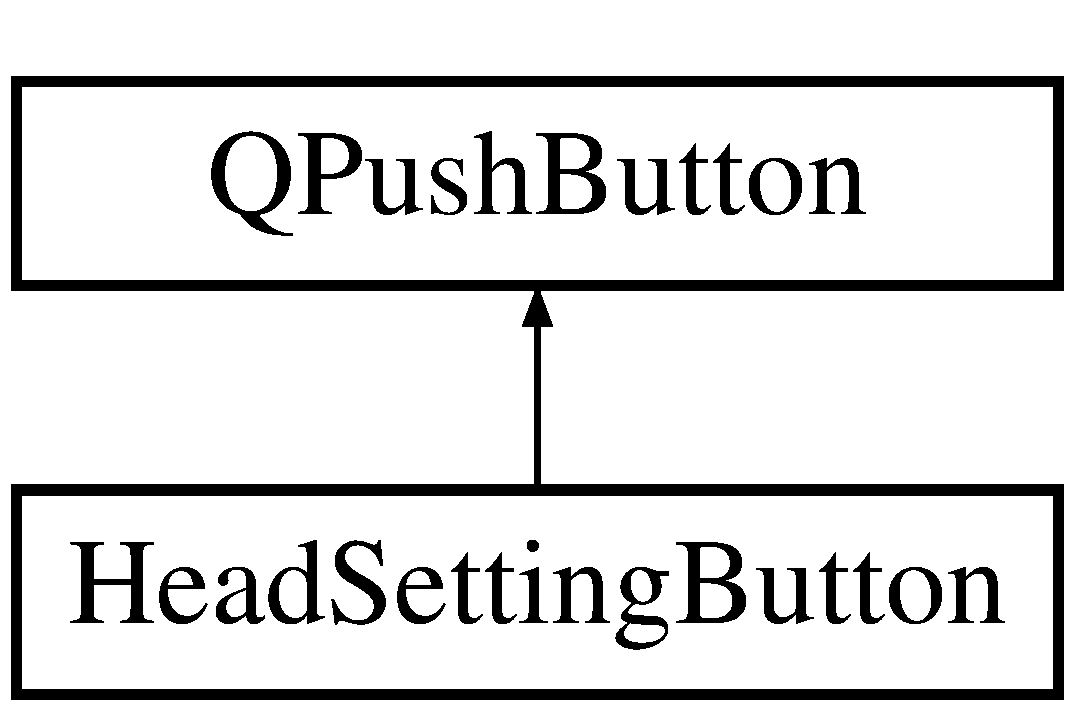
\includegraphics[height=2.000000cm]{classHeadSettingButton}
\end{center}
\end{figure}
\subsubsection*{Signals}
\begin{DoxyCompactItemize}
\item 
void \mbox{\hyperlink{classHeadSettingButton_acd459234032c48f57a7a964c214ca0bf}{setting\+Button\+Cliced}} (int \mbox{\hyperlink{classHeadSettingButton_ad583fdc744e019c787477694427cdde0}{index}})
\end{DoxyCompactItemize}
\subsubsection*{Public Member Functions}
\begin{DoxyCompactItemize}
\item 
\mbox{\hyperlink{classHeadSettingButton_a098c4f2a77e710e4034b085923b1a556}{Head\+Setting\+Button}} (unsigned int input\+Number, Q\+Widget $\ast$parent=0)
\item 
void \mbox{\hyperlink{classHeadSettingButton_a9fe218e02cfc06467659eabbd7f4a794}{set\+Icon\+Path}} (Q\+String path)
\end{DoxyCompactItemize}
\subsubsection*{Private Slots}
\begin{DoxyCompactItemize}
\item 
void \mbox{\hyperlink{classHeadSettingButton_a9b462518ae3b222488fbec936c39c294}{this\+Clicked}} ()
\end{DoxyCompactItemize}
\subsubsection*{Private Attributes}
\begin{DoxyCompactItemize}
\item 
unsigned int \mbox{\hyperlink{classHeadSettingButton_ad583fdc744e019c787477694427cdde0}{index}}
\end{DoxyCompactItemize}


\subsubsection{Constructor \& Destructor Documentation}
\mbox{\Hypertarget{classHeadSettingButton_a098c4f2a77e710e4034b085923b1a556}\label{classHeadSettingButton_a098c4f2a77e710e4034b085923b1a556}} 
\index{Head\+Setting\+Button@{Head\+Setting\+Button}!Head\+Setting\+Button@{Head\+Setting\+Button}}
\index{Head\+Setting\+Button@{Head\+Setting\+Button}!Head\+Setting\+Button@{Head\+Setting\+Button}}
{\footnotesize\ttfamily Head\+Setting\+Button\+::\+\texorpdfstring{Head\+Setting\+Button}{HeadSettingButton} (\begin{DoxyParamCaption}\item[{unsigned int}]{input\+Number,  }\item[{Q\+Widget $\ast$}]{parent = {\ttfamily 0} }\end{DoxyParamCaption}){\ttfamily [inline]}} - constructor of class. Create widget and set \hyperlink{classHeadSettingButton_ad583fdc744e019c787477694427cdde0}{index} variable

\subsubsection{Member Function Documentation}
\mbox{\Hypertarget{classHeadSettingButton_a9fe218e02cfc06467659eabbd7f4a794}\label{classHeadSettingButton_a9fe218e02cfc06467659eabbd7f4a794}} 
\index{Head\+Setting\+Button@{Head\+Setting\+Button}!set\+Icon\+Path@{set\+Icon\+Path}}
\index{set\+Icon\+Path@{set\+Icon\+Path}!Head\+Setting\+Button@{Head\+Setting\+Button}}
{\footnotesize\ttfamily void Head\+Setting\+Button\+::\texorpdfstring{set\+Icon\+Path}{setIconPath} (\begin{DoxyParamCaption}\item[{Q\+String}]{path }\end{DoxyParamCaption}){\ttfamily [inline]}} - function to update icon on button.

\mbox{\Hypertarget{classHeadSettingButton_acd459234032c48f57a7a964c214ca0bf}\label{classHeadSettingButton_acd459234032c48f57a7a964c214ca0bf}} 
\index{Head\+Setting\+Button@{Head\+Setting\+Button}!setting\+Button\+Cliced@{setting\+Button\+Cliced}}
\index{setting\+Button\+Cliced@{setting\+Button\+Cliced}!Head\+Setting\+Button@{Head\+Setting\+Button}}
{\footnotesize\ttfamily void Head\+Setting\+Button\+::\texorpdfstring{setting\+Button\+Cliced}{settingButtonCliced} (\begin{DoxyParamCaption}\item[{int}]{index }\end{DoxyParamCaption}){\ttfamily [signal]}} signal what emitted by \hyperlink{classHeadSettingButton_a9b462518ae3b222488fbec936c39c294}{this\+Clicked} function and handle in parent object by \hyperlink{classMainWindow_ae823008e53cce4636c1776d86c946cf5}{head\+Setting\+Request}(...) function. 

\mbox{\Hypertarget{classHeadSettingButton_a9b462518ae3b222488fbec936c39c294}\label{classHeadSettingButton_a9b462518ae3b222488fbec936c39c294}} 
\index{Head\+Setting\+Button@{Head\+Setting\+Button}!this\+Clicked@{this\+Clicked}}
\index{this\+Clicked@{this\+Clicked}!Head\+Setting\+Button@{Head\+Setting\+Button}}
{\footnotesize\ttfamily void Head\+Setting\+Button\+::\texorpdfstring{this\+Clicked}{thisClicked} (\begin{DoxyParamCaption}{ }\end{DoxyParamCaption}){\ttfamily [inline]}, {\ttfamily [private]}, {\ttfamily [slot]}} - function which called by standard \textit{Q\+Push\+Button} clicked() signal. 

\subsubsection{Member Data Documentation}
\mbox{\Hypertarget{classHeadSettingButton_ad583fdc744e019c787477694427cdde0}\label{classHeadSettingButton_ad583fdc744e019c787477694427cdde0}} 
\index{Head\+Setting\+Button@{Head\+Setting\+Button}!index@{index}}
\index{index@{index}!Head\+Setting\+Button@{Head\+Setting\+Button}}
{\footnotesize\ttfamily unsigned int Head\+Setting\+Button\+::\texorpdfstring{index}{index}{\ttfamily [private]}}

The documentation for this class was generated from the following file\+:\begin{DoxyCompactItemize}
\item 
\mbox{\hyperlink{headform_8h}{headform.\+h}}\end{DoxyCompactItemize}
\newpage
\hypertarget{classIndexerLiftSettings}{}\subsection{Indexer\+Lift\+Settings Class Reference}
\label{classIndexerLiftSettings}\index{Indexer\+Lift\+Settings@{Indexer\+Lift\+Settings}}


{\ttfamily \#include $<$settings.\+h$>$}

\subsubsection*{Classes}
\begin{DoxyCompactItemize}
\item 
struct \mbox{\hyperlink{structIndexerLiftSettings_1_1IndexParameters__}{Index\+Parameters\+\_\+}}
\item 
struct \mbox{\hyperlink{structIndexerLiftSettings_1_1LiftParameters__}{Lift\+Parameters\+\_\+}}
\end{DoxyCompactItemize}
\subsubsection*{Public Types}
\begin{DoxyCompactItemize}
\item 
enum \mbox{\hyperlink{classIndexerLiftSettings_a3ab6e8bfdd1aaed688b1cca43dd7c913}{Devices}} \{
\begin{DoxyCompactItemize} \item\mbox{\hyperlink{classIndexerLiftSettings_a3ab6e8bfdd1aaed688b1cca43dd7c913a39a548178de68c2a3e7658fb85a56106}{Lift\+Device}} = 0x0002, 
\item\mbox{\hyperlink{classIndexerLiftSettings_a3ab6e8bfdd1aaed688b1cca43dd7c913af9df5c0187f5e281e965ff067ec76581}{Indexer\+Device}} = 0x0001
 \end{DoxyCompactItemize}\}
\item 
enum \mbox{\hyperlink{classIndexerLiftSettings_a116f9cef65d6fcc44ea04a2458ccd5a2}{Indexer\+Lift\+Data\+Places}} \{ 
\begin{DoxyCompactItemize}
\item\mbox{\hyperlink{classIndexerLiftSettings_a116f9cef65d6fcc44ea04a2458ccd5a2a151ea8edc8114bb78ece10e9858c3537}{Index\+Home\+Offset}} = 0x01, 
\item\mbox{\hyperlink{classIndexerLiftSettings_a116f9cef65d6fcc44ea04a2458ccd5a2a256876ab80cd7e9f9067f818b2b07dd0}{Index\+Dist\+Offcet}} = 0x02, 
\item\mbox{\hyperlink{classIndexerLiftSettings_a116f9cef65d6fcc44ea04a2458ccd5a2a8eea1737b7266266d501ed2cc273bd03}{Index\+Speed}} = 0x03, 
\item\mbox{\hyperlink{classIndexerLiftSettings_a116f9cef65d6fcc44ea04a2458ccd5a2a4a19a82f0e80f8dcde0783e22e2697d2}{Index\+Direction}} = 0x04, 
\item\mbox{\hyperlink{classIndexerLiftSettings_a116f9cef65d6fcc44ea04a2458ccd5a2ac1524a3717768f68bfdee53c0b6d9ad4}{Index\+Step\+Time\+Delay}} = 0x06, 
\item\mbox{\hyperlink{classIndexerLiftSettings_a116f9cef65d6fcc44ea04a2458ccd5a2a98a1621bf4c939ac36f37c30bed6da43}{Lift\+Delay\+Down}} = 0x1C, 
\item\mbox{\hyperlink{classIndexerLiftSettings_a116f9cef65d6fcc44ea04a2458ccd5a2ac0271452c6890ade65149a2613adbd58}{Lift\+Delay\+Up}} = 0x07, 
\item\mbox{\hyperlink{classIndexerLiftSettings_a116f9cef65d6fcc44ea04a2458ccd5a2abe1bb0f5775199c03ab8dc8b5a51d0a9}{Index\+Distance}} = 0x08, 
\item\mbox{\hyperlink{classIndexerLiftSettings_a116f9cef65d6fcc44ea04a2458ccd5a2a66c5c7a90572973dee3606e62bae51da}{Index\+Last\+Revolv\+Warm}} = 0x09, 
\item\mbox{\hyperlink{classIndexerLiftSettings_a116f9cef65d6fcc44ea04a2458ccd5a2aac6ca5cd57cca87f10268db6527e8442}{Index\+Acceleration}} = 0x0A, 
\item\mbox{\hyperlink{classIndexerLiftSettings_a116f9cef65d6fcc44ea04a2458ccd5a2aa11ee9a20d44c72639f159fcc660f3f2}{Index\+Acceleration\+Ret}} = 0x0B, 
\item\mbox{\hyperlink{classIndexerLiftSettings_a116f9cef65d6fcc44ea04a2458ccd5a2aeacb918f16b01f08a3ce32715adcb530}{Index\+Speed\+Ret}} = 0x0D, 
\item\mbox{\hyperlink{classIndexerLiftSettings_a116f9cef65d6fcc44ea04a2458ccd5a2a5fb01934908f5879af2dd4b044943ce2}{Warning\+Time}} = 0x0E, 
\item\mbox{\hyperlink{classIndexerLiftSettings_a116f9cef65d6fcc44ea04a2458ccd5a2a8192201a86b56410dfd09fd2b9800fa1}{Lift\+Home\+Offcet}} = 0x15, 
\item\mbox{\hyperlink{classIndexerLiftSettings_a116f9cef65d6fcc44ea04a2458ccd5a2a2ba128cb6dfe2c80448c6578cc543872}{Lift\+Distance}} = 0x16, 
\item\mbox{\hyperlink{classIndexerLiftSettings_a116f9cef65d6fcc44ea04a2458ccd5a2ab38ed4c8a800ac897f0339f0aef56dcc}{Lift\+Speed}} = 0x17, 
\item\mbox{\hyperlink{classIndexerLiftSettings_a116f9cef65d6fcc44ea04a2458ccd5a2a864489dda212f5a39e7df91499450822}{Lift\+Acceleration}} = 0x18, 
\item\mbox{\hyperlink{classIndexerLiftSettings_a116f9cef65d6fcc44ea04a2458ccd5a2a3f25c659b07800fb5f565359ed27ba6a}{Load\+Head\+State}} = 0x1F
 \end{DoxyCompactItemize}\}
\item 
enum \mbox{\hyperlink{classIndexerLiftSettings_a1cdeb18e15c35f26a2979194c6db9452}{Indexer\+Commands\+En\+\_\+}} \{ 
\begin{DoxyCompactItemize}
\item\mbox{\hyperlink{classIndexerLiftSettings_a1cdeb18e15c35f26a2979194c6db9452a8a5db6c30f6075cf5d320deee8d15fed}{Machine\+\_\+\+Reset}} = 0x0001, 
\item\mbox{\hyperlink{classIndexerLiftSettings_a1cdeb18e15c35f26a2979194c6db9452a9ab75d3e05b86c537f251b62f539317b}{Machine\+\_\+\+Home}} = 0x0009, 
\item\mbox{\hyperlink{classIndexerLiftSettings_a1cdeb18e15c35f26a2979194c6db9452a0df4113ba596d97fb0b3c7c0beee8e50}{Index\+Lock}} = 0x000A, 
\item\mbox{\hyperlink{classIndexerLiftSettings_a1cdeb18e15c35f26a2979194c6db9452ab7e7809b193ce7b9b4cc44aa1990972c}{Index\+Un\+Lock}} = 0x000A, 
\item\mbox{\hyperlink{classIndexerLiftSettings_a1cdeb18e15c35f26a2979194c6db9452afd53a7da44594fbce348e39b173d4e79}{Move\+Up\+\_\+\+Down}} = 0x0006, 
\item\mbox{\hyperlink{classIndexerLiftSettings_a1cdeb18e15c35f26a2979194c6db9452a801b1e41af74addb06b4ff09b8d8cd53}{Move\+Left}} = 0x0005, 
\item\mbox{\hyperlink{classIndexerLiftSettings_a1cdeb18e15c35f26a2979194c6db9452a661bb94b6f94ef440de35fa75caf31b4}{Move\+Right}} = 0x0007, 
\item\mbox{\hyperlink{classIndexerLiftSettings_a1cdeb18e15c35f26a2979194c6db9452a4b674c236e8750e8251ae7c745778246}{Move\+Left\+Half}} = 0x0005, 
\item\mbox{\hyperlink{classIndexerLiftSettings_a1cdeb18e15c35f26a2979194c6db9452a3cf954c86851ef8b0651e2ce819d0133}{Move\+Right\+Half}} = 0x0007, 
\item\mbox{\hyperlink{classIndexerLiftSettings_a1cdeb18e15c35f26a2979194c6db9452a847b891eb365b54d93f042a382bb68bb}{Move\+Full\+\_\+\+Half}} = 0x0004, 
\item\mbox{\hyperlink{classIndexerLiftSettings_a1cdeb18e15c35f26a2979194c6db9452a7817bc36050d9ab3837d3980c3571823}{Auto\+\_\+\+Manual}} = 0x0008, 
\item\mbox{\hyperlink{classIndexerLiftSettings_a1cdeb18e15c35f26a2979194c6db9452a272ba966d584c46e633fbbffb34f9d6a}{Print\+Start}} = 0x000B, 
\item\mbox{\hyperlink{classIndexerLiftSettings_a1cdeb18e15c35f26a2979194c6db9452a33952d02298706bf400ae5b63a11a8ec}{Print\+Stop}} = 0x000B, 
\item\mbox{\hyperlink{classIndexerLiftSettings_a1cdeb18e15c35f26a2979194c6db9452aa0e77b4e4baa11b333114b484c1e01b2}{Air\+Release}} = 0x005A, 
\item\mbox{\hyperlink{classIndexerLiftSettings_a1cdeb18e15c35f26a2979194c6db9452a29a08ace010cd85dc1fdc0ff236b4a52}{Easy\+Setup}} = 0x08, 
\item\mbox{\hyperlink{classIndexerLiftSettings_a1cdeb18e15c35f26a2979194c6db9452a6a15b2f6b11726fedaab365c734bb35c}{Index\+Move\+Home}} = 0x005B, 
\item\mbox{\hyperlink{classIndexerLiftSettings_a1cdeb18e15c35f26a2979194c6db9452a4c1aee5c9ac7d395ea3de3101117609f}{Index\+Move\+End}} = 0x005C, 
\item\mbox{\hyperlink{classIndexerLiftSettings_a1cdeb18e15c35f26a2979194c6db9452af6bd0d1521e5060028d6d36f63c5b8e7}{Lift\+Move\+Home}} = 0x00B8, 
\item\mbox{\hyperlink{classIndexerLiftSettings_a1cdeb18e15c35f26a2979194c6db9452adfe78fdba789cb03023ba4d142e3efab}{Lift\+Move\+End}} = 0x00B9, 
\item\mbox{\hyperlink{classIndexerLiftSettings_a1cdeb18e15c35f26a2979194c6db9452a3a0d3424bd5c37e15efcbf4dbd26bbba}{Index\+Dir\+Change}} = 0x005D
 \end{DoxyCompactItemize}
 \}
\item 
typedef struct \mbox{\hyperlink{structIndexerLiftSettings_1_1LiftParameters__}{Indexer\+Lift\+Settings\+::\+Lift\+Parameters\+\_\+}} \mbox{\hyperlink{classIndexerLiftSettings_a83fd6fc58021bc526b681c1ce840f686}{Lift\+Parameters}}
\item 
typedef struct \mbox{\hyperlink{structIndexerLiftSettings_1_1IndexParameters__}{Indexer\+Lift\+Settings\+::\+Index\+Parameters\+\_\+}} \mbox{\hyperlink{classIndexerLiftSettings_a6b75f15b6abc72b9070642cb8b5408ca}{Index\+Parameters}}
\item 
typedef enum \mbox{\hyperlink{classIndexerLiftSettings_a1cdeb18e15c35f26a2979194c6db9452}{Indexer\+Lift\+Settings\+::\+Indexer\+Commands\+En\+\_\+}} \mbox{\hyperlink{classIndexerLiftSettings_ad0959473f792741cadaa262730f5a463}{Indexer\+Commands\+En}}
\end{DoxyCompactItemize}
\subsubsection*{Public Member Functions}
\begin{DoxyCompactItemize}
\item 
\mbox{\hyperlink{classIndexerLiftSettings_aa334786f67544a57de7253b930eb3528}{Indexer\+Lift\+Settings}} (\mbox{\hyperlink{classIndexerLiftSettings_a6b75f15b6abc72b9070642cb8b5408ca}{Index\+Parameters}} ind\+Param, \mbox{\hyperlink{classIndexerLiftSettings_a83fd6fc58021bc526b681c1ce840f686}{Lift\+Parameters}} lif\+Param)
\item 
\mbox{\hyperlink{classIndexerLiftSettings_ad3adde70e8138f9f775ff9177ce290fe}{Indexer\+Lift\+Settings}} ()
\item 
void \mbox{\hyperlink{classIndexerLiftSettings_ade953aea43325531e7889e71d45d6e65}{from\+Byte\+Array}} (Q\+Byte\+Array ind\+Param\+Arr, Q\+Byte\+Array lif\+Param\+Arr)
\end{DoxyCompactItemize}
\subsubsection*{Public Attributes}
\begin{DoxyCompactItemize}
\item 
\mbox{\hyperlink{classIndexerLiftSettings_a6b75f15b6abc72b9070642cb8b5408ca}{Index\+Parameters}} \mbox{\hyperlink{classIndexerLiftSettings_a09875fa890744d5de30f06b2d580bb24}{indexer\+Param}}
\item 
\mbox{\hyperlink{classIndexerLiftSettings_a83fd6fc58021bc526b681c1ce840f686}{Lift\+Parameters}} \mbox{\hyperlink{classIndexerLiftSettings_ae9649b8642d20d02892fc4abaad687f7}{lift\+Param}}
\end{DoxyCompactItemize}


\subsubsection{Member Typedef Documentation}
\mbox{\Hypertarget{classIndexerLiftSettings_ad0959473f792741cadaa262730f5a463}\label{classIndexerLiftSettings_ad0959473f792741cadaa262730f5a463}} 
\index{Indexer\+Lift\+Settings@{Indexer\+Lift\+Settings}!Indexer\+Commands\+En@{Indexer\+Commands\+En}}
\index{Indexer\+Commands\+En@{Indexer\+Commands\+En}!Indexer\+Lift\+Settings@{Indexer\+Lift\+Settings}}
{\footnotesize\ttfamily typedef enum \mbox{\hyperlink{classIndexerLiftSettings_a1cdeb18e15c35f26a2979194c6db9452}{Indexer\+Lift\+Settings\+::\+Indexer\+Commands\+En\+\_\+}} \mbox{\hyperlink{classIndexerLiftSettings_ad0959473f792741cadaa262730f5a463}{Indexer\+Lift\+Settings\+::\texorpdfstring{Indexer\+Commands\+En}{IndexerCommandsEn}}}}

\mbox{\Hypertarget{classIndexerLiftSettings_a6b75f15b6abc72b9070642cb8b5408ca}\label{classIndexerLiftSettings_a6b75f15b6abc72b9070642cb8b5408ca}} 
\index{Indexer\+Lift\+Settings@{Indexer\+Lift\+Settings}!Index\+Parameters@{Index\+Parameters}}
\index{Index\+Parameters@{Index\+Parameters}!Indexer\+Lift\+Settings@{Indexer\+Lift\+Settings}}
{\footnotesize\ttfamily typedef struct \mbox{\hyperlink{structIndexerLiftSettings_1_1IndexParameters__}{Indexer\+Lift\+Settings\+::\+Index\+Parameters\+\_\+}} \mbox{\hyperlink{classIndexerLiftSettings_a6b75f15b6abc72b9070642cb8b5408ca}{Indexer\+Lift\+Settings\+::\texorpdfstring{Index\+Parameters}{IndexParameters}}}}

\mbox{\Hypertarget{classIndexerLiftSettings_a83fd6fc58021bc526b681c1ce840f686}\label{classIndexerLiftSettings_a83fd6fc58021bc526b681c1ce840f686}} 
\index{Indexer\+Lift\+Settings@{Indexer\+Lift\+Settings}!Lift\+Parameters@{Lift\+Parameters}}
\index{Lift\+Parameters@{Lift\+Parameters}!Indexer\+Lift\+Settings@{Indexer\+Lift\+Settings}}
{\footnotesize\ttfamily typedef struct \mbox{\hyperlink{structIndexerLiftSettings_1_1LiftParameters__}{Indexer\+Lift\+Settings\+::\+Lift\+Parameters\+\_\+}} \mbox{\hyperlink{classIndexerLiftSettings_a83fd6fc58021bc526b681c1ce840f686}{Indexer\+Lift\+Settings\+::\texorpdfstring{Lift\+Parameters}{LiftParameters}}}}



\subsubsection{Member Enumeration Documentation}
\mbox{\Hypertarget{classIndexerLiftSettings_a3ab6e8bfdd1aaed688b1cca43dd7c913}\label{classIndexerLiftSettings_a3ab6e8bfdd1aaed688b1cca43dd7c913}} 
\index{Indexer\+Lift\+Settings@{Indexer\+Lift\+Settings}!Devices@{Devices}}
\index{Devices@{Devices}!Indexer\+Lift\+Settings@{Indexer\+Lift\+Settings}}
{\footnotesize\ttfamily enum \mbox{\hyperlink{classIndexerLiftSettings_a3ab6e8bfdd1aaed688b1cca43dd7c913}{Indexer\+Lift\+Settings\+::\texorpdfstring{Devices}{Devices}}}} - enumerator which contain device addresses of lift and indexer. 

\begin{DoxyEnumFields}{Enumerator}
\raisebox{\heightof{T}}[0pt][0pt]{\index{Lift\+Device@{Lift\+Device}!Indexer\+Lift\+Settings@{Indexer\+Lift\+Settings}}\index{Indexer\+Lift\+Settings@{Indexer\+Lift\+Settings}!Lift\+Device@{Lift\+Device}}}\mbox{\Hypertarget{classIndexerLiftSettings_a3ab6e8bfdd1aaed688b1cca43dd7c913a39a548178de68c2a3e7658fb85a56106}\label{classIndexerLiftSettings_a3ab6e8bfdd1aaed688b1cca43dd7c913a39a548178de68c2a3e7658fb85a56106}} 
Lift\+Device&0x0002\\
\hline

\raisebox{\heightof{T}}[0pt][0pt]{\index{Indexer\+Device@{Indexer\+Device}!Indexer\+Lift\+Settings@{Indexer\+Lift\+Settings}}\index{Indexer\+Lift\+Settings@{Indexer\+Lift\+Settings}!Indexer\+Device@{Indexer\+Device}}}\mbox{\Hypertarget{classIndexerLiftSettings_a3ab6e8bfdd1aaed688b1cca43dd7c913af9df5c0187f5e281e965ff067ec76581}\label{classIndexerLiftSettings_a3ab6e8bfdd1aaed688b1cca43dd7c913af9df5c0187f5e281e965ff067ec76581}} 
Indexer\+Device&0x0001\\
\hline

\end{DoxyEnumFields}
\mbox{\Hypertarget{classIndexerLiftSettings_a1cdeb18e15c35f26a2979194c6db9452}\label{classIndexerLiftSettings_a1cdeb18e15c35f26a2979194c6db9452}} 
\index{Indexer\+Lift\+Settings@{Indexer\+Lift\+Settings}!Indexer\+Commands\+En\+\_\+@{Indexer\+Commands\+En\+\_\+}}
\index{Indexer\+Commands\+En\+\_\+@{Indexer\+Commands\+En\+\_\+}!Indexer\+Lift\+Settings@{Indexer\+Lift\+Settings}}
{\footnotesize\ttfamily enum \mbox{\hyperlink{classIndexerLiftSettings_a1cdeb18e15c35f26a2979194c6db9452}{Indexer\+Lift\+Settings\+::\texorpdfstring{Indexer\+Commands\+En\+\_\+}{IndexerCommandsEn\_}}}} - enumerator, which written to create names of data what must be send to execute commands for indexer and lift device.

\begin{DoxyEnumFields}{Enumerator}
\raisebox{\heightof{T}}[0pt][0pt]{\index{Machine\+\_\+\+Reset@{Machine\+\_\+\+Reset}!Indexer\+Lift\+Settings@{Indexer\+Lift\+Settings}}\index{Indexer\+Lift\+Settings@{Indexer\+Lift\+Settings}!Machine\+\_\+\+Reset@{Machine\+\_\+\+Reset}}}\mbox{\Hypertarget{classIndexerLiftSettings_a1cdeb18e15c35f26a2979194c6db9452a8a5db6c30f6075cf5d320deee8d15fed}\label{classIndexerLiftSettings_a1cdeb18e15c35f26a2979194c6db9452a8a5db6c30f6075cf5d320deee8d15fed}} 
Machine\+\_\+\+Reset&0x0001\\
\hline

\raisebox{\heightof{T}}[0pt][0pt]{\index{Machine\+\_\+\+Home@{Machine\+\_\+\+Home}!Indexer\+Lift\+Settings@{Indexer\+Lift\+Settings}}\index{Indexer\+Lift\+Settings@{Indexer\+Lift\+Settings}!Machine\+\_\+\+Home@{Machine\+\_\+\+Home}}}\mbox{\Hypertarget{classIndexerLiftSettings_a1cdeb18e15c35f26a2979194c6db9452a9ab75d3e05b86c537f251b62f539317b}\label{classIndexerLiftSettings_a1cdeb18e15c35f26a2979194c6db9452a9ab75d3e05b86c537f251b62f539317b}} 
Machine\+\_\+\+Home&0x0009\\
\hline

\raisebox{\heightof{T}}[0pt][0pt]{\index{Index\+Lock@{Index\+Lock}!Indexer\+Lift\+Settings@{Indexer\+Lift\+Settings}}\index{Indexer\+Lift\+Settings@{Indexer\+Lift\+Settings}!Index\+Lock@{Index\+Lock}}}\mbox{\Hypertarget{classIndexerLiftSettings_a1cdeb18e15c35f26a2979194c6db9452a0df4113ba596d97fb0b3c7c0beee8e50}\label{classIndexerLiftSettings_a1cdeb18e15c35f26a2979194c6db9452a0df4113ba596d97fb0b3c7c0beee8e50}} 
Index\+Lock&0x000A\\
\hline

\raisebox{\heightof{T}}[0pt][0pt]{\index{Index\+Un\+Lock@{Index\+Un\+Lock}!Indexer\+Lift\+Settings@{Indexer\+Lift\+Settings}}\index{Indexer\+Lift\+Settings@{Indexer\+Lift\+Settings}!Index\+Un\+Lock@{Index\+Un\+Lock}}}\mbox{\Hypertarget{classIndexerLiftSettings_a1cdeb18e15c35f26a2979194c6db9452ab7e7809b193ce7b9b4cc44aa1990972c}\label{classIndexerLiftSettings_a1cdeb18e15c35f26a2979194c6db9452ab7e7809b193ce7b9b4cc44aa1990972c}} 
Index\+Un\+Lock&0x000A\\
\hline

\raisebox{\heightof{T}}[0pt][0pt]{\index{Move\+Up\+\_\+\+Down@{Move\+Up\+\_\+\+Down}!Indexer\+Lift\+Settings@{Indexer\+Lift\+Settings}}\index{Indexer\+Lift\+Settings@{Indexer\+Lift\+Settings}!Move\+Up\+\_\+\+Down@{Move\+Up\+\_\+\+Down}}}\mbox{\Hypertarget{classIndexerLiftSettings_a1cdeb18e15c35f26a2979194c6db9452afd53a7da44594fbce348e39b173d4e79}\label{classIndexerLiftSettings_a1cdeb18e15c35f26a2979194c6db9452afd53a7da44594fbce348e39b173d4e79}} 
Move\+Up\+\_\+\+Down&0x0006\\
\hline

\raisebox{\heightof{T}}[0pt][0pt]{\index{Move\+Left@{Move\+Left}!Indexer\+Lift\+Settings@{Indexer\+Lift\+Settings}}\index{Indexer\+Lift\+Settings@{Indexer\+Lift\+Settings}!Move\+Left@{Move\+Left}}}\mbox{\Hypertarget{classIndexerLiftSettings_a1cdeb18e15c35f26a2979194c6db9452a801b1e41af74addb06b4ff09b8d8cd53}\label{classIndexerLiftSettings_a1cdeb18e15c35f26a2979194c6db9452a801b1e41af74addb06b4ff09b8d8cd53}} 
Move\+Left&0x0005\\
\hline

\raisebox{\heightof{T}}[0pt][0pt]{\index{Move\+Right@{Move\+Right}!Indexer\+Lift\+Settings@{Indexer\+Lift\+Settings}}\index{Indexer\+Lift\+Settings@{Indexer\+Lift\+Settings}!Move\+Right@{Move\+Right}}}\mbox{\Hypertarget{classIndexerLiftSettings_a1cdeb18e15c35f26a2979194c6db9452a661bb94b6f94ef440de35fa75caf31b4}\label{classIndexerLiftSettings_a1cdeb18e15c35f26a2979194c6db9452a661bb94b6f94ef440de35fa75caf31b4}} 
Move\+Right&0x0007\\
\hline

\raisebox{\heightof{T}}[0pt][0pt]{\index{Move\+Left\+Half@{Move\+Left\+Half}!Indexer\+Lift\+Settings@{Indexer\+Lift\+Settings}}\index{Indexer\+Lift\+Settings@{Indexer\+Lift\+Settings}!Move\+Left\+Half@{Move\+Left\+Half}}}\mbox{\Hypertarget{classIndexerLiftSettings_a1cdeb18e15c35f26a2979194c6db9452a4b674c236e8750e8251ae7c745778246}\label{classIndexerLiftSettings_a1cdeb18e15c35f26a2979194c6db9452a4b674c236e8750e8251ae7c745778246}} 
Move\+Left\+Half&0x0005\\
\hline

\raisebox{\heightof{T}}[0pt][0pt]{\index{Move\+Right\+Half@{Move\+Right\+Half}!Indexer\+Lift\+Settings@{Indexer\+Lift\+Settings}}\index{Indexer\+Lift\+Settings@{Indexer\+Lift\+Settings}!Move\+Right\+Half@{Move\+Right\+Half}}}\mbox{\Hypertarget{classIndexerLiftSettings_a1cdeb18e15c35f26a2979194c6db9452a3cf954c86851ef8b0651e2ce819d0133}\label{classIndexerLiftSettings_a1cdeb18e15c35f26a2979194c6db9452a3cf954c86851ef8b0651e2ce819d0133}} 
Move\+Right\+Half&0x0007\\
\hline

\raisebox{\heightof{T}}[0pt][0pt]{\index{Move\+Full\+\_\+\+Half@{Move\+Full\+\_\+\+Half}!Indexer\+Lift\+Settings@{Indexer\+Lift\+Settings}}\index{Indexer\+Lift\+Settings@{Indexer\+Lift\+Settings}!Move\+Full\+\_\+\+Half@{Move\+Full\+\_\+\+Half}}}\mbox{\Hypertarget{classIndexerLiftSettings_a1cdeb18e15c35f26a2979194c6db9452a847b891eb365b54d93f042a382bb68bb}\label{classIndexerLiftSettings_a1cdeb18e15c35f26a2979194c6db9452a847b891eb365b54d93f042a382bb68bb}} 
Move\+Full\+\_\+\+Half&0x0004\\
\hline

\raisebox{\heightof{T}}[0pt][0pt]{\index{Auto\+\_\+\+Manual@{Auto\+\_\+\+Manual}!Indexer\+Lift\+Settings@{Indexer\+Lift\+Settings}}\index{Indexer\+Lift\+Settings@{Indexer\+Lift\+Settings}!Auto\+\_\+\+Manual@{Auto\+\_\+\+Manual}}}\mbox{\Hypertarget{classIndexerLiftSettings_a1cdeb18e15c35f26a2979194c6db9452a7817bc36050d9ab3837d3980c3571823}\label{classIndexerLiftSettings_a1cdeb18e15c35f26a2979194c6db9452a7817bc36050d9ab3837d3980c3571823}} 
Auto\+\_\+\+Manual&0x0008\\
\hline

\raisebox{\heightof{T}}[0pt][0pt]{\index{Print\+Start@{Print\+Start}!Indexer\+Lift\+Settings@{Indexer\+Lift\+Settings}}\index{Indexer\+Lift\+Settings@{Indexer\+Lift\+Settings}!Print\+Start@{Print\+Start}}}\mbox{\Hypertarget{classIndexerLiftSettings_a1cdeb18e15c35f26a2979194c6db9452a272ba966d584c46e633fbbffb34f9d6a}\label{classIndexerLiftSettings_a1cdeb18e15c35f26a2979194c6db9452a272ba966d584c46e633fbbffb34f9d6a}} 
Print\+Start&0x000B\\
\hline

\raisebox{\heightof{T}}[0pt][0pt]{\index{Print\+Stop@{Print\+Stop}!Indexer\+Lift\+Settings@{Indexer\+Lift\+Settings}}\index{Indexer\+Lift\+Settings@{Indexer\+Lift\+Settings}!Print\+Stop@{Print\+Stop}}}\mbox{\Hypertarget{classIndexerLiftSettings_a1cdeb18e15c35f26a2979194c6db9452a33952d02298706bf400ae5b63a11a8ec}\label{classIndexerLiftSettings_a1cdeb18e15c35f26a2979194c6db9452a33952d02298706bf400ae5b63a11a8ec}} 
Print\+Stop&0x000B\\
\hline

\raisebox{\heightof{T}}[0pt][0pt]{\index{Air\+Release@{Air\+Release}!Indexer\+Lift\+Settings@{Indexer\+Lift\+Settings}}\index{Indexer\+Lift\+Settings@{Indexer\+Lift\+Settings}!Air\+Release@{Air\+Release}}}\mbox{\Hypertarget{classIndexerLiftSettings_a1cdeb18e15c35f26a2979194c6db9452aa0e77b4e4baa11b333114b484c1e01b2}\label{classIndexerLiftSettings_a1cdeb18e15c35f26a2979194c6db9452aa0e77b4e4baa11b333114b484c1e01b2}} 
Air\+Release&0x005A\\
\hline

\raisebox{\heightof{T}}[0pt][0pt]{\index{Easy\+Setup@{Easy\+Setup}!Indexer\+Lift\+Settings@{Indexer\+Lift\+Settings}}\index{Indexer\+Lift\+Settings@{Indexer\+Lift\+Settings}!Easy\+Setup@{Easy\+Setup}}}\mbox{\Hypertarget{classIndexerLiftSettings_a1cdeb18e15c35f26a2979194c6db9452a29a08ace010cd85dc1fdc0ff236b4a52}\label{classIndexerLiftSettings_a1cdeb18e15c35f26a2979194c6db9452a29a08ace010cd85dc1fdc0ff236b4a52}} 
Easy\+Setup&0x0008\\
\hline

\raisebox{\heightof{T}}[0pt][0pt]{\index{Index\+Move\+Home@{Index\+Move\+Home}!Indexer\+Lift\+Settings@{Indexer\+Lift\+Settings}}\index{Indexer\+Lift\+Settings@{Indexer\+Lift\+Settings}!Index\+Move\+Home@{Index\+Move\+Home}}}\mbox{\Hypertarget{classIndexerLiftSettings_a1cdeb18e15c35f26a2979194c6db9452a6a15b2f6b11726fedaab365c734bb35c}\label{classIndexerLiftSettings_a1cdeb18e15c35f26a2979194c6db9452a6a15b2f6b11726fedaab365c734bb35c}} 
Index\+Move\+Home&0x005B\\
\hline

\raisebox{\heightof{T}}[0pt][0pt]{\index{Index\+Move\+End@{Index\+Move\+End}!Indexer\+Lift\+Settings@{Indexer\+Lift\+Settings}}\index{Indexer\+Lift\+Settings@{Indexer\+Lift\+Settings}!Index\+Move\+End@{Index\+Move\+End}}}\mbox{\Hypertarget{classIndexerLiftSettings_a1cdeb18e15c35f26a2979194c6db9452a4c1aee5c9ac7d395ea3de3101117609f}\label{classIndexerLiftSettings_a1cdeb18e15c35f26a2979194c6db9452a4c1aee5c9ac7d395ea3de3101117609f}} 
Index\+Move\+End&0x005C\\
\hline

\raisebox{\heightof{T}}[0pt][0pt]{\index{Lift\+Move\+Home@{Lift\+Move\+Home}!Indexer\+Lift\+Settings@{Indexer\+Lift\+Settings}}\index{Indexer\+Lift\+Settings@{Indexer\+Lift\+Settings}!Lift\+Move\+Home@{Lift\+Move\+Home}}}\mbox{\Hypertarget{classIndexerLiftSettings_a1cdeb18e15c35f26a2979194c6db9452af6bd0d1521e5060028d6d36f63c5b8e7}\label{classIndexerLiftSettings_a1cdeb18e15c35f26a2979194c6db9452af6bd0d1521e5060028d6d36f63c5b8e7}} 
Lift\+Move\+Home&0x00B8\\
\hline

\raisebox{\heightof{T}}[0pt][0pt]{\index{Lift\+Move\+End@{Lift\+Move\+End}!Indexer\+Lift\+Settings@{Indexer\+Lift\+Settings}}\index{Indexer\+Lift\+Settings@{Indexer\+Lift\+Settings}!Lift\+Move\+End@{Lift\+Move\+End}}}\mbox{\Hypertarget{classIndexerLiftSettings_a1cdeb18e15c35f26a2979194c6db9452adfe78fdba789cb03023ba4d142e3efab}\label{classIndexerLiftSettings_a1cdeb18e15c35f26a2979194c6db9452adfe78fdba789cb03023ba4d142e3efab}} 
Lift\+Move\+End&0x00B9\\
\hline

\raisebox{\heightof{T}}[0pt][0pt]{\index{Index\+Dir\+Change@{Index\+Dir\+Change}!Indexer\+Lift\+Settings@{Indexer\+Lift\+Settings}}\index{Indexer\+Lift\+Settings@{Indexer\+Lift\+Settings}!Index\+Dir\+Change@{Index\+Dir\+Change}}}\mbox{\Hypertarget{classIndexerLiftSettings_a1cdeb18e15c35f26a2979194c6db9452a3a0d3424bd5c37e15efcbf4dbd26bbba}\label{classIndexerLiftSettings_a1cdeb18e15c35f26a2979194c6db9452a3a0d3424bd5c37e15efcbf4dbd26bbba}} 
Index\+Dir\+Change&0x005D\\
\hline

\end{DoxyEnumFields}
\mbox{\Hypertarget{classIndexerLiftSettings_a116f9cef65d6fcc44ea04a2458ccd5a2}\label{classIndexerLiftSettings_a116f9cef65d6fcc44ea04a2458ccd5a2}} 
\index{Indexer\+Lift\+Settings@{Indexer\+Lift\+Settings}!Indexer\+Lift\+Data\+Places@{Indexer\+Lift\+Data\+Places}}
\index{Indexer\+Lift\+Data\+Places@{Indexer\+Lift\+Data\+Places}!Indexer\+Lift\+Settings@{Indexer\+Lift\+Settings}}
{\footnotesize\ttfamily enum \mbox{\hyperlink{classIndexerLiftSettings_a116f9cef65d6fcc44ea04a2458ccd5a2}{Indexer\+Lift\+Settings\+::\texorpdfstring{Indexer\+Lift\+Data\+Places}{IndexerLiftDataPlaces}}}} - Enumerator describe address of data places for indexer and lift device. Name of enumerator item describe parameter which are sends to PCB.

\begin{DoxyEnumFields}{Enumerator}
\raisebox{\heightof{T}}[0pt][0pt]{\index{Index\+Home\+Offset@{Index\+Home\+Offset}!Indexer\+Lift\+Settings@{Indexer\+Lift\+Settings}}\index{Indexer\+Lift\+Settings@{Indexer\+Lift\+Settings}!Index\+Home\+Offset@{Index\+Home\+Offset}}}\mbox{\Hypertarget{classIndexerLiftSettings_a116f9cef65d6fcc44ea04a2458ccd5a2a151ea8edc8114bb78ece10e9858c3537}\label{classIndexerLiftSettings_a116f9cef65d6fcc44ea04a2458ccd5a2a151ea8edc8114bb78ece10e9858c3537}} 
Index\+Home\+Offset&0x01\\
\hline

\raisebox{\heightof{T}}[0pt][0pt]{\index{Index\+Dist\+Offcet@{Index\+Dist\+Offcet}!Indexer\+Lift\+Settings@{Indexer\+Lift\+Settings}}\index{Indexer\+Lift\+Settings@{Indexer\+Lift\+Settings}!Index\+Dist\+Offcet@{Index\+Dist\+Offcet}}}\mbox{\Hypertarget{classIndexerLiftSettings_a116f9cef65d6fcc44ea04a2458ccd5a2a256876ab80cd7e9f9067f818b2b07dd0}\label{classIndexerLiftSettings_a116f9cef65d6fcc44ea04a2458ccd5a2a256876ab80cd7e9f9067f818b2b07dd0}} 
Index\+Dist\+Offcet&0x02\\
\hline

\raisebox{\heightof{T}}[0pt][0pt]{\index{Index\+Speed@{Index\+Speed}!Indexer\+Lift\+Settings@{Indexer\+Lift\+Settings}}\index{Indexer\+Lift\+Settings@{Indexer\+Lift\+Settings}!Index\+Speed@{Index\+Speed}}}\mbox{\Hypertarget{classIndexerLiftSettings_a116f9cef65d6fcc44ea04a2458ccd5a2a8eea1737b7266266d501ed2cc273bd03}\label{classIndexerLiftSettings_a116f9cef65d6fcc44ea04a2458ccd5a2a8eea1737b7266266d501ed2cc273bd03}} 
Index\+Speed&0x03\\
\hline

\raisebox{\heightof{T}}[0pt][0pt]{\index{Index\+Direction@{Index\+Direction}!Indexer\+Lift\+Settings@{Indexer\+Lift\+Settings}}\index{Indexer\+Lift\+Settings@{Indexer\+Lift\+Settings}!Index\+Direction@{Index\+Direction}}}\mbox{\Hypertarget{classIndexerLiftSettings_a116f9cef65d6fcc44ea04a2458ccd5a2a4a19a82f0e80f8dcde0783e22e2697d2}\label{classIndexerLiftSettings_a116f9cef65d6fcc44ea04a2458ccd5a2a4a19a82f0e80f8dcde0783e22e2697d2}} 
Index\+Direction&0x04\\
\hline

\raisebox{\heightof{T}}[0pt][0pt]{\index{Index\+Step\+Time\+Delay@{Index\+Step\+Time\+Delay}!Indexer\+Lift\+Settings@{Indexer\+Lift\+Settings}}\index{Indexer\+Lift\+Settings@{Indexer\+Lift\+Settings}!Index\+Step\+Time\+Delay@{Index\+Step\+Time\+Delay}}}\mbox{\Hypertarget{classIndexerLiftSettings_a116f9cef65d6fcc44ea04a2458ccd5a2ac1524a3717768f68bfdee53c0b6d9ad4}\label{classIndexerLiftSettings_a116f9cef65d6fcc44ea04a2458ccd5a2ac1524a3717768f68bfdee53c0b6d9ad4}} 
Index\+Step\+Time\+Delay&0x06\\
\hline

\raisebox{\heightof{T}}[0pt][0pt]{\index{Lift\+Delay\+Down@{Lift\+Delay\+Down}!Indexer\+Lift\+Settings@{Indexer\+Lift\+Settings}}\index{Indexer\+Lift\+Settings@{Indexer\+Lift\+Settings}!Lift\+Delay\+Down@{Lift\+Delay\+Down}}}\mbox{\Hypertarget{classIndexerLiftSettings_a116f9cef65d6fcc44ea04a2458ccd5a2a98a1621bf4c939ac36f37c30bed6da43}\label{classIndexerLiftSettings_a116f9cef65d6fcc44ea04a2458ccd5a2a98a1621bf4c939ac36f37c30bed6da43}} 
Lift\+Delay\+Down&0x1C\\
\hline

\raisebox{\heightof{T}}[0pt][0pt]{\index{Lift\+Delay\+Up@{Lift\+Delay\+Up}!Indexer\+Lift\+Settings@{Indexer\+Lift\+Settings}}\index{Indexer\+Lift\+Settings@{Indexer\+Lift\+Settings}!Lift\+Delay\+Up@{Lift\+Delay\+Up}}}\mbox{\Hypertarget{classIndexerLiftSettings_a116f9cef65d6fcc44ea04a2458ccd5a2ac0271452c6890ade65149a2613adbd58}\label{classIndexerLiftSettings_a116f9cef65d6fcc44ea04a2458ccd5a2ac0271452c6890ade65149a2613adbd58}} 
Lift\+Delay\+Up&0x07\\
\hline

\raisebox{\heightof{T}}[0pt][0pt]{\index{Index\+Distance@{Index\+Distance}!Indexer\+Lift\+Settings@{Indexer\+Lift\+Settings}}\index{Indexer\+Lift\+Settings@{Indexer\+Lift\+Settings}!Index\+Distance@{Index\+Distance}}}\mbox{\Hypertarget{classIndexerLiftSettings_a116f9cef65d6fcc44ea04a2458ccd5a2abe1bb0f5775199c03ab8dc8b5a51d0a9}\label{classIndexerLiftSettings_a116f9cef65d6fcc44ea04a2458ccd5a2abe1bb0f5775199c03ab8dc8b5a51d0a9}} 
Index\+Distance&0x08\\
\hline

\raisebox{\heightof{T}}[0pt][0pt]{\index{Index\+Last\+Revolv\+Warm@{Index\+Last\+Revolv\+Warm}!Indexer\+Lift\+Settings@{Indexer\+Lift\+Settings}}\index{Indexer\+Lift\+Settings@{Indexer\+Lift\+Settings}!Index\+Last\+Revolv\+Warm@{Index\+Last\+Revolv\+Warm}}}\mbox{\Hypertarget{classIndexerLiftSettings_a116f9cef65d6fcc44ea04a2458ccd5a2a66c5c7a90572973dee3606e62bae51da}\label{classIndexerLiftSettings_a116f9cef65d6fcc44ea04a2458ccd5a2a66c5c7a90572973dee3606e62bae51da}} 
Index\+Last\+Revolv\+Warm&0x09\\
\hline

\raisebox{\heightof{T}}[0pt][0pt]{\index{Index\+Acceleration@{Index\+Acceleration}!Indexer\+Lift\+Settings@{Indexer\+Lift\+Settings}}\index{Indexer\+Lift\+Settings@{Indexer\+Lift\+Settings}!Index\+Acceleration@{Index\+Acceleration}}}\mbox{\Hypertarget{classIndexerLiftSettings_a116f9cef65d6fcc44ea04a2458ccd5a2aac6ca5cd57cca87f10268db6527e8442}\label{classIndexerLiftSettings_a116f9cef65d6fcc44ea04a2458ccd5a2aac6ca5cd57cca87f10268db6527e8442}} 
Index\+Acceleration&0x0A\\
\hline

\raisebox{\heightof{T}}[0pt][0pt]{\index{Index\+Acceleration\+Ret@{Index\+Acceleration\+Ret}!Indexer\+Lift\+Settings@{Indexer\+Lift\+Settings}}\index{Indexer\+Lift\+Settings@{Indexer\+Lift\+Settings}!Index\+Acceleration\+Ret@{Index\+Acceleration\+Ret}}}\mbox{\Hypertarget{classIndexerLiftSettings_a116f9cef65d6fcc44ea04a2458ccd5a2aa11ee9a20d44c72639f159fcc660f3f2}\label{classIndexerLiftSettings_a116f9cef65d6fcc44ea04a2458ccd5a2aa11ee9a20d44c72639f159fcc660f3f2}} 
Index\+Acceleration\+Ret&0x0B\\
\hline

\raisebox{\heightof{T}}[0pt][0pt]{\index{Index\+Speed\+Ret@{Index\+Speed\+Ret}!Indexer\+Lift\+Settings@{Indexer\+Lift\+Settings}}\index{Indexer\+Lift\+Settings@{Indexer\+Lift\+Settings}!Index\+Speed\+Ret@{Index\+Speed\+Ret}}}\mbox{\Hypertarget{classIndexerLiftSettings_a116f9cef65d6fcc44ea04a2458ccd5a2aeacb918f16b01f08a3ce32715adcb530}\label{classIndexerLiftSettings_a116f9cef65d6fcc44ea04a2458ccd5a2aeacb918f16b01f08a3ce32715adcb530}} 
Index\+Speed\+Ret&0x0D\\
\hline

\raisebox{\heightof{T}}[0pt][0pt]{\index{Warning\+Time@{Warning\+Time}!Indexer\+Lift\+Settings@{Indexer\+Lift\+Settings}}\index{Indexer\+Lift\+Settings@{Indexer\+Lift\+Settings}!Warning\+Time@{Warning\+Time}}}\mbox{\Hypertarget{classIndexerLiftSettings_a116f9cef65d6fcc44ea04a2458ccd5a2a5fb01934908f5879af2dd4b044943ce2}\label{classIndexerLiftSettings_a116f9cef65d6fcc44ea04a2458ccd5a2a5fb01934908f5879af2dd4b044943ce2}} 
Warning\+Time&0x0E\\
\hline

\raisebox{\heightof{T}}[0pt][0pt]{\index{Lift\+Home\+Offcet@{Lift\+Home\+Offcet}!Indexer\+Lift\+Settings@{Indexer\+Lift\+Settings}}\index{Indexer\+Lift\+Settings@{Indexer\+Lift\+Settings}!Lift\+Home\+Offcet@{Lift\+Home\+Offcet}}}\mbox{\Hypertarget{classIndexerLiftSettings_a116f9cef65d6fcc44ea04a2458ccd5a2a8192201a86b56410dfd09fd2b9800fa1}\label{classIndexerLiftSettings_a116f9cef65d6fcc44ea04a2458ccd5a2a8192201a86b56410dfd09fd2b9800fa1}} 
Lift\+Home\+Offcet&0x15\\
\hline

\raisebox{\heightof{T}}[0pt][0pt]{\index{Lift\+Distance@{Lift\+Distance}!Indexer\+Lift\+Settings@{Indexer\+Lift\+Settings}}\index{Indexer\+Lift\+Settings@{Indexer\+Lift\+Settings}!Lift\+Distance@{Lift\+Distance}}}\mbox{\Hypertarget{classIndexerLiftSettings_a116f9cef65d6fcc44ea04a2458ccd5a2a2ba128cb6dfe2c80448c6578cc543872}\label{classIndexerLiftSettings_a116f9cef65d6fcc44ea04a2458ccd5a2a2ba128cb6dfe2c80448c6578cc543872}} 
Lift\+Distance&0x16\\
\hline

\raisebox{\heightof{T}}[0pt][0pt]{\index{Lift\+Speed@{Lift\+Speed}!Indexer\+Lift\+Settings@{Indexer\+Lift\+Settings}}\index{Indexer\+Lift\+Settings@{Indexer\+Lift\+Settings}!Lift\+Speed@{Lift\+Speed}}}\mbox{\Hypertarget{classIndexerLiftSettings_a116f9cef65d6fcc44ea04a2458ccd5a2ab38ed4c8a800ac897f0339f0aef56dcc}\label{classIndexerLiftSettings_a116f9cef65d6fcc44ea04a2458ccd5a2ab38ed4c8a800ac897f0339f0aef56dcc}} 
Lift\+Speed&0x17\\
\hline

\raisebox{\heightof{T}}[0pt][0pt]{\index{Lift\+Acceleration@{Lift\+Acceleration}!Indexer\+Lift\+Settings@{Indexer\+Lift\+Settings}}\index{Indexer\+Lift\+Settings@{Indexer\+Lift\+Settings}!Lift\+Acceleration@{Lift\+Acceleration}}}\mbox{\Hypertarget{classIndexerLiftSettings_a116f9cef65d6fcc44ea04a2458ccd5a2a864489dda212f5a39e7df91499450822}\label{classIndexerLiftSettings_a116f9cef65d6fcc44ea04a2458ccd5a2a864489dda212f5a39e7df91499450822}} 
Lift\+Acceleration&0x18\\
\hline

\raisebox{\heightof{T}}[0pt][0pt]{\index{Load\+Head\+State@{Load\+Head\+State}!Indexer\+Lift\+Settings@{Indexer\+Lift\+Settings}}\index{Indexer\+Lift\+Settings@{Indexer\+Lift\+Settings}!Load\+Head\+State@{Load\+Head\+State}}}\mbox{\Hypertarget{classIndexerLiftSettings_a116f9cef65d6fcc44ea04a2458ccd5a2a3f25c659b07800fb5f565359ed27ba6a}\label{classIndexerLiftSettings_a116f9cef65d6fcc44ea04a2458ccd5a2a3f25c659b07800fb5f565359ed27ba6a}} 
Load\+Head\+State&0x1F\\
\hline

\end{DoxyEnumFields}


\subsubsection{Constructor \& Destructor Documentation}
\mbox{\Hypertarget{classIndexerLiftSettings_aa334786f67544a57de7253b930eb3528}\label{classIndexerLiftSettings_aa334786f67544a57de7253b930eb3528}} 
\index{Indexer\+Lift\+Settings@{Indexer\+Lift\+Settings}!Indexer\+Lift\+Settings@{Indexer\+Lift\+Settings}}
\index{Indexer\+Lift\+Settings@{Indexer\+Lift\+Settings}!Indexer\+Lift\+Settings@{Indexer\+Lift\+Settings}}
{\footnotesize\ttfamily Indexer\+Lift\+Settings\+::\texorpdfstring{Indexer\+Lift\+Settings}{IndexerLiftSettings}{\footnotesize\ttfamily [1/2]} (\begin{DoxyParamCaption}\item[{\mbox{\hyperlink{classIndexerLiftSettings_a6b75f15b6abc72b9070642cb8b5408ca}{Indexer\+Lift\+Settings\+::\+Index\+Parameters}}}]{ind\+Param,  }\item[{\mbox{\hyperlink{classIndexerLiftSettings_a83fd6fc58021bc526b681c1ce840f686}{Indexer\+Lift\+Settings\+::\+Lift\+Parameters}}}]{lif\+Param }\end{DoxyParamCaption})} - class constructor with data initialization. Initialize \hyperlink{classIndexerLiftSettings_a09875fa890744d5de30f06b2d580bb24}{indexer\+Param} and \hyperlink{classIndexerLiftSettings_ae9649b8642d20d02892fc4abaad687f7}{lift\+Param} with given data.

\mbox{\Hypertarget{classIndexerLiftSettings_ad3adde70e8138f9f775ff9177ce290fe}\label{classIndexerLiftSettings_ad3adde70e8138f9f775ff9177ce290fe}} 
\index{Indexer\+Lift\+Settings@{Indexer\+Lift\+Settings}!Indexer\+Lift\+Settings@{Indexer\+Lift\+Settings}}
\index{Indexer\+Lift\+Settings@{Indexer\+Lift\+Settings}!Indexer\+Lift\+Settings@{Indexer\+Lift\+Settings}}
{\footnotesize\ttfamily Indexer\+Lift\+Settings\+::\texorpdfstring{Indexer\+Lift\+Settings}{IndexerLiftSettings}{\footnotesize\ttfamily [2/2]} (\begin{DoxyParamCaption}{ }\end{DoxyParamCaption})} - empty class constructor. Initialize \hyperlink{classIndexerLiftSettings_a09875fa890744d5de30f06b2d580bb24}{indexer\+Param} and \hyperlink{classIndexerLiftSettings_ae9649b8642d20d02892fc4abaad687f7}{lift\+Param} with default parameters.

\subsubsection{Member Function Documentation}
\mbox{\Hypertarget{classIndexerLiftSettings_ade953aea43325531e7889e71d45d6e65}\label{classIndexerLiftSettings_ade953aea43325531e7889e71d45d6e65}} \index{Indexer\+Lift\+Settings@{Indexer\+Lift\+Settings}!from\+Byte\+Array@{from\+Byte\+Array}}\index{from\+Byte\+Array@{from\+Byte\+Array}!Indexer\+Lift\+Settings@{Indexer\+Lift\+Settings}}{\footnotesize\ttfamily void Indexer\+Lift\+Settings\+::\texorpdfstring{from\+Byte\+Array}{fromByteArray} (\begin{DoxyParamCaption}\item[{Q\+Byte\+Array}]{ind\+Param\+Arr,  }\item[{Q\+Byte\+Array}]{lif\+Param\+Arr }\end{DoxyParamCaption})} - fill fields of \hyperlink{classIndexerLiftSettings_a09875fa890744d5de30f06b2d580bb24}{indexer\+Param} and \hyperlink{classIndexerLiftSettings_ae9649b8642d20d02892fc4abaad687f7}{lift\+Param} with data parsed from given \mbox{\textit{Q\+Byte\+Array}'s}.

\subsubsection{Member Data Documentation}
\mbox{\Hypertarget{classIndexerLiftSettings_a09875fa890744d5de30f06b2d580bb24}\label{classIndexerLiftSettings_a09875fa890744d5de30f06b2d580bb24}} 
\index{Indexer\+Lift\+Settings@{Indexer\+Lift\+Settings}!indexer\+Param@{indexer\+Param}}
\index{indexer\+Param@{indexer\+Param}!Indexer\+Lift\+Settings@{Indexer\+Lift\+Settings}}
{\footnotesize\ttfamily \mbox{\hyperlink{classIndexerLiftSettings_a6b75f15b6abc72b9070642cb8b5408ca}{Index\+Parameters}} Indexer\+Lift\+Settings\+::\texorpdfstring{indexer\+Param}{indexerParam}}

\mbox{\Hypertarget{classIndexerLiftSettings_ae9649b8642d20d02892fc4abaad687f7}\label{classIndexerLiftSettings_ae9649b8642d20d02892fc4abaad687f7}} 
\index{Indexer\+Lift\+Settings@{Indexer\+Lift\+Settings}!lift\+Param@{lift\+Param}}
\index{lift\+Param@{lift\+Param}!Indexer\+Lift\+Settings@{Indexer\+Lift\+Settings}}
{\footnotesize\ttfamily \mbox{\hyperlink{classIndexerLiftSettings_a83fd6fc58021bc526b681c1ce840f686}{Lift\+Parameters}} Indexer\+Lift\+Settings\+::\texorpdfstring{lift\+Param}{liftParam}}


The documentation for this class was generated from the following files\+:\begin{DoxyCompactItemize}
\item 
\mbox{\hyperlink{settings_8h}{settings.\+h}}\item 
\mbox{\hyperlink{settings_8cpp}{settings.\+cpp}}\end{DoxyCompactItemize}
\newpage
\hypertarget{unionRegister_1_1IndexerReg__}{}\subsection{Register\+:\+:Indexer\+Reg\+\_\+ Union Reference}
\label{unionRegister_1_1IndexerReg__}\index{Register\+::\+Indexer\+Reg\+\_\+@{Register\+::\+Indexer\+Reg\+\_\+}}


{\ttfamily \#include $<$settings.\+h$>$}

\subsubsection*{Classes}
\begin{DoxyCompactItemize}
\item 
struct \mbox{\hyperlink{structRegister_1_1IndexerReg___1_1reg}{reg}}
\end{DoxyCompactItemize}
\subsubsection*{Public Attributes}
\begin{DoxyCompactItemize}
\item 
struct \mbox{\hyperlink{structRegister_1_1IndexerReg___1_1reg}{Register\+::\+Indexer\+Reg\+\_\+\+::reg}} \mbox{\hyperlink{unionRegister_1_1IndexerReg___a21a03f333ef5c8e16708cf38d22d5abb}{field}}
\item 
\mbox{\hyperlink{settings_8h_a017dd44e68049ffdd31500a8cd01ba68}{uint16\+\_\+t}} \mbox{\hyperlink{unionRegister_1_1IndexerReg___ab61397dfa5cf6bbc29d9642c3875967f}{mem\+Beg}}
\end{DoxyCompactItemize}


\subsubsection{Member Data Documentation}
\mbox{\Hypertarget{unionRegister_1_1IndexerReg___a21a03f333ef5c8e16708cf38d22d5abb}\label{unionRegister_1_1IndexerReg___a21a03f333ef5c8e16708cf38d22d5abb}} 
\index{Register\+::\+Indexer\+Reg\+\_\+@{Register\+::\+Indexer\+Reg\+\_\+}!field@{field}}
\index{field@{field}!Register\+::\+Indexer\+Reg\+\_\+@{Register\+::\+Indexer\+Reg\+\_\+}}
{\footnotesize\ttfamily struct \mbox{\hyperlink{structRegister_1_1IndexerReg___1_1reg}{Register\+::\+Indexer\+Reg\+\_\+\+::reg}} Register\+::\+Indexer\+Reg\+\_\+\+::\texorpdfstring{field}{field}} - fields of \hyperlink{structRegister_1_1IndexerReg___1_1reg}{Register\+::\+Indexer\+Reg\+\_\+\+::reg} structure to give possibility to access to memory by name.

\mbox{\Hypertarget{unionRegister_1_1IndexerReg___ab61397dfa5cf6bbc29d9642c3875967f}\label{unionRegister_1_1IndexerReg___ab61397dfa5cf6bbc29d9642c3875967f}} 
\index{Register\+::\+Indexer\+Reg\+\_\+@{Register\+::\+Indexer\+Reg\+\_\+}!mem\+Beg@{mem\+Beg}}
\index{mem\+Beg@{mem\+Beg}!Register\+::\+Indexer\+Reg\+\_\+@{Register\+::\+Indexer\+Reg\+\_\+}}
{\footnotesize\ttfamily \mbox{\hyperlink{settings_8h_a017dd44e68049ffdd31500a8cd01ba68}{uint16\+\_\+t}} Register\+::\+Indexer\+Reg\+\_\+\+::\texorpdfstring{mem\+Beg}{memBeg}} - variable to notice beginning of memory region of structure.

The documentation for this union was generated from the following file\+:\begin{DoxyCompactItemize}
\item 
\mbox{\hyperlink{settings_8h}{settings.\+h}}\end{DoxyCompactItemize}
\newpage
\hypertarget{classIndexerSettingDialog}{}\subsection{Indexer\+Setting\+Dialog Class Reference}
\label{classIndexerSettingDialog}\index{Indexer\+Setting\+Dialog@{Indexer\+Setting\+Dialog}}


{\ttfamily \#include $<$indexersettingdialog.\+h$>$}

Inheritance diagram for Indexer\+Setting\+Dialog\+:\begin{figure}[H]
\begin{center}
\leavevmode
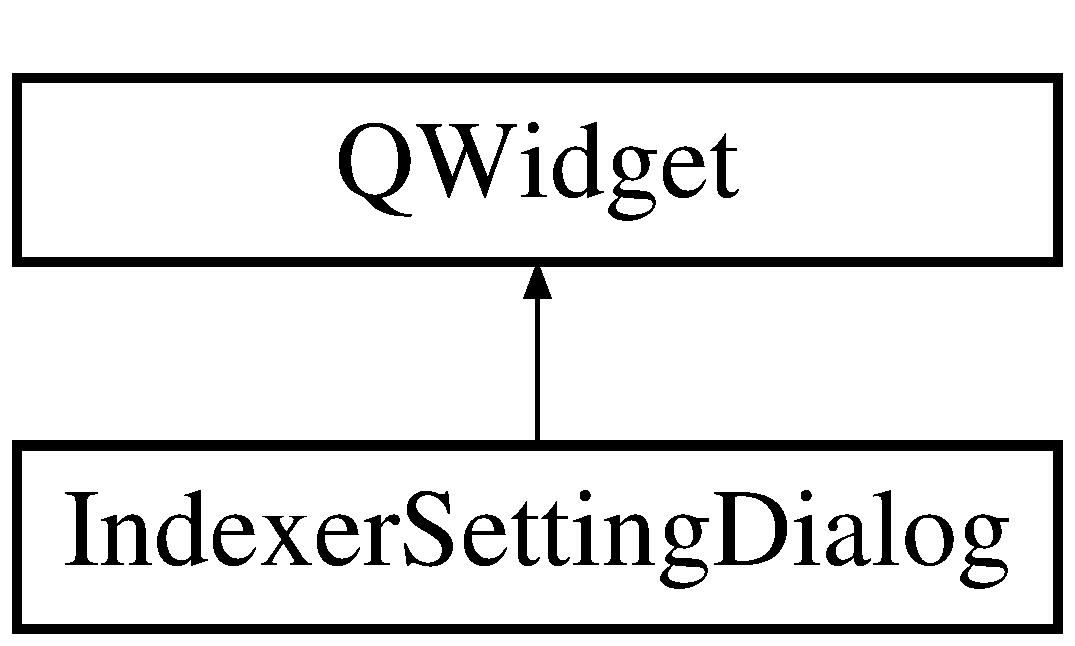
\includegraphics[height=2.000000cm]{classIndexerSettingDialog}
\end{center}
\end{figure}
\subsubsection*{Signals}
\begin{DoxyCompactItemize}
\item 
void \mbox{\hyperlink{classIndexerSettingDialog_a231edf60936e09b15972951f8a7751e7}{indexer\+Param\+Changed}} (Q\+Byte\+Array index\+Param\+Arr)
\item 
void \mbox{\hyperlink{classIndexerSettingDialog_a40d9bb1a05d0afb9bb8a0191f611d78c}{lift\+Param\+Changed}} (Q\+Byte\+Array lift\+Param\+Arr)
\item 
void \mbox{\hyperlink{classIndexerSettingDialog_adbccfa0b79b30c4a5373e183f7828524}{send\+Command}} (Q\+Byte\+Array command)
\item 
void \mbox{\hyperlink{classIndexerSettingDialog_a8d5a19a8948b46f84de79d40775f05c5}{lift\+Distance\+Changed}} (float distance)
\end{DoxyCompactItemize}
\subsubsection*{Public Member Functions}
\begin{DoxyCompactItemize}
\item 
\mbox{\hyperlink{classIndexerSettingDialog_ad2c64f92d2d17bc3d8045dd84eeb71e8}{Indexer\+Setting\+Dialog}} (Q\+Widget $\ast$parent=0)
\item 
\mbox{\hyperlink{classIndexerSettingDialog_a87b6ba4152cb2b6a02a93e502d7b64ff}{$\sim$\+Indexer\+Setting\+Dialog}} ()
\item 
void \mbox{\hyperlink{classIndexerSettingDialog_a2b0fb04ec9698b7bc82a69ae3d379a1b}{set\+Registers}} (\mbox{\hyperlink{classRegister}{Register}} $\ast$reg)
\item 
void \mbox{\hyperlink{classIndexerSettingDialog_a3b3ff00a9731a94931be5f2c9590fa37}{set\+Indexer\+Setting}} (bool disconnect=true)
\item 
void \mbox{\hyperlink{classIndexerSettingDialog_ae98cd594c5da327549e306a2ec09718e}{set\+Lift\+Setting}} (bool disconnect=true)
\item 
void \mbox{\hyperlink{classIndexerSettingDialog_aea4b170b962c7e2e319565f3fde73b14}{set\+Indexer\+Setting}} (\mbox{\hyperlink{classIndexerLiftSettings_a6b75f15b6abc72b9070642cb8b5408ca}{Indexer\+Lift\+Settings\+::\+Index\+Parameters}} index\+Param, bool disconnect=true)
\item 
void \mbox{\hyperlink{classIndexerSettingDialog_aa8ef316cb26c8c1c2149581679ca9646}{set\+Lift\+Setting}} (\mbox{\hyperlink{classIndexerLiftSettings_a83fd6fc58021bc526b681c1ce840f686}{Indexer\+Lift\+Settings\+::\+Lift\+Parameters}} lift\+Param, bool disconnect=true)
\item 
void \mbox{\hyperlink{classIndexerSettingDialog_a12036cd566ddbb3581bf7a526bf0d18f}{set\+Lift\+Distance}} (float distance, int \mbox{\hyperlink{classIndexerSettingDialog_a9dfafe2970aeba611a1736a3797cc3f3}{lift\+Gear\+Ratio}})
\item 
float \mbox{\hyperlink{classIndexerSettingDialog_a436f30e8ab3af6ea4b3a2389c6711fd4}{get\+Lift\+Distance}} ()
\item 
void \mbox{\hyperlink{classIndexerSettingDialog_a3b2f9533b1c72aecd3d36bb4d175859f}{set\+Lift\+Gear\+Ratio}} (\mbox{\hyperlink{settings_8h_a4196118492a3b1493c81f250e90af775}{uint32\+\_\+t}} \mbox{\hyperlink{classIndexerSettingDialog_a9dfafe2970aeba611a1736a3797cc3f3}{lift\+Gear\+Ratio}})
\end{DoxyCompactItemize}
\subsubsection*{Protected Member Functions}
\begin{DoxyCompactItemize}
\item 
bool \mbox{\hyperlink{classIndexerSettingDialog_a20a34151fec7c14426e8ff8b210d1cc9}{event}} (Q\+Event $\ast$e)
\item 
bool \mbox{\hyperlink{classIndexerSettingDialog_af096cfd78afd37d27487dd383ed30188}{event\+Filter}} (Q\+Object $\ast$watched, Q\+Event $\ast$\mbox{\hyperlink{classIndexerSettingDialog_a20a34151fec7c14426e8ff8b210d1cc9}{event}})
\item 
void \mbox{\hyperlink{classIndexerSettingDialog_a04091d56225031b1ca05b769f2bba105}{show\+Event}} (Q\+Show\+Event $\ast$ev)
\item 
void \mbox{\hyperlink{classIndexerSettingDialog_a2140c46d3d12396442388a3c42ba8e83}{change\+Event}} (Q\+Event $\ast$\mbox{\hyperlink{classIndexerSettingDialog_a20a34151fec7c14426e8ff8b210d1cc9}{event}})
\end{DoxyCompactItemize}
\subsubsection*{Private Slots}
\begin{DoxyCompactItemize}
\item 
void \mbox{\hyperlink{classIndexerSettingDialog_a4d7f2f508e87ac980d21557f5a18a216}{connect\+All}} ()
\item 
void \mbox{\hyperlink{classIndexerSettingDialog_a1a3a501889727528a4f432b233556760}{disconnect\+All}} ()
\item 
void \mbox{\hyperlink{classIndexerSettingDialog_a32e867b5d070ed40929837ebc4b45a78}{accept}} ()
\item 
void \mbox{\hyperlink{classIndexerSettingDialog_a36fd628fd129e8fab31e7876085d1a71}{reject}} ()
\item 
void \mbox{\hyperlink{classIndexerSettingDialog_a1843f10a012a547c32953866ecece54b}{event\+Filter\+Setup}} ()
\item 
void \mbox{\hyperlink{classIndexerSettingDialog_af2f32d79f004b22b713fa30fa0952364}{d\+Spin\+Box\+Index\+Distance\+\_\+value\+Changed}} (double arg1)
\item 
void \mbox{\hyperlink{classIndexerSettingDialog_a589985949822923031a396092d4f24c0}{spin\+Box\+Index\+Home\+Offset\+\_\+value\+Changed}} (double arg1)
\item 
void \mbox{\hyperlink{classIndexerSettingDialog_ae65f25d6b260c3534ef2e03745e54a07}{spin\+Box\+Index\+Distance\+Offcet\+\_\+value\+Changed}} (double arg1)
\item 
void \mbox{\hyperlink{classIndexerSettingDialog_a52510947409dd78b5262bfc320ce85d0}{spin\+Box\+Index\+Speed\+\_\+value\+Changed}} (double arg1)
\item 
void \mbox{\hyperlink{classIndexerSettingDialog_a89996434374b3f24dd26ebf9aae81de4}{d\+Spin\+Box\+Index\+Accel\+\_\+value\+Changed}} (double arg1)
\item 
void \mbox{\hyperlink{classIndexerSettingDialog_a077a9cde82a08f7ae66654cf26a452bd}{spin\+Boxindex\+Speed\+Ret\+\_\+value\+Changed}} (double arg1)
\item 
void \mbox{\hyperlink{classIndexerSettingDialog_a7084aa1c59b526f1e3ea07b2e9a23b56}{d\+Spin\+Box\+Index\+Accel\+Ret\+\_\+value\+Changed}} (double arg1)
\item 
void \mbox{\hyperlink{classIndexerSettingDialog_a02d9d9a3c2b76d6576334a48752be9d7}{d\+Spin\+Box\+Lift\+Down\+Delay\+\_\+value\+Changed}} (double arg1)
\item 
void \mbox{\hyperlink{classIndexerSettingDialog_a596e2bdb49c0681bd06d847497d20cad}{d\+Spin\+Box\+Lift\+Up\+Delay\+\_\+value\+Changed}} (double arg1)
\item 
void \mbox{\hyperlink{classIndexerSettingDialog_a4cc32d94f2a3d8ed8cf99665f3d95d99}{d\+Spin\+Box\+Lift\+Distance\+\_\+value\+Changed}} (double arg1)
\item 
void \mbox{\hyperlink{classIndexerSettingDialog_a84a27fcd118a8208944a216cd88022c9}{spin\+Box\+Lift\+Home\+Offset\+\_\+value\+Changed}} (double arg1)
\item 
void \mbox{\hyperlink{classIndexerSettingDialog_a3632876be4c809b96b93d402044b3716}{spin\+Box\+Lift\+Speed\+\_\+value\+Changed}} (double arg1)
\item 
void \mbox{\hyperlink{classIndexerSettingDialog_a6a2a10523b6a1611763249e16bd65100}{d\+Spin\+Box\+Lift\+Accel\+\_\+value\+Changed}} (double arg1)
\item 
void \mbox{\hyperlink{classIndexerSettingDialog_ac0ae2808aaa375d27ca2caafe47c2c35}{on\+\_\+p\+Button\+Lift\+Move\+\_\+clicked}} ()
\item 
void \mbox{\hyperlink{classIndexerSettingDialog_a1dcf2f19ff38e28177ecad8f430af3c6}{on\+\_\+p\+Button\+Lift\+Home\+\_\+clicked}} ()
\item 
void \mbox{\hyperlink{classIndexerSettingDialog_a30f8761c69279bed9085dce50ec83422}{on\+\_\+p\+Button\+Index\+Move\+\_\+clicked}} ()
\item 
void \mbox{\hyperlink{classIndexerSettingDialog_a0d983ff2b43c6ad2d501a0c4e00d88e5}{on\+\_\+p\+Button\+Index\+Home\+\_\+clicked}} ()
\end{DoxyCompactItemize}
\subsubsection*{Private Attributes}
\begin{DoxyCompactItemize}
\item 
Ui\+::\+Indexer\+Setting\+Dialog $\ast$ \mbox{\hyperlink{classIndexerSettingDialog_ad5a0497f91a33e699cdbd912a6089776}{ui}}
\item 
bool \mbox{\hyperlink{classIndexerSettingDialog_aa781b93909330f9c60b4494555b39b4b}{accept\+On\+Deactilation\+En}}
\item 
bool \mbox{\hyperlink{classIndexerSettingDialog_a14a7ea545fca4efbe05799efe767f678}{accept\+Enable}}
\item 
\mbox{\hyperlink{settings_8h_a4196118492a3b1493c81f250e90af775}{uint32\+\_\+t}} \mbox{\hyperlink{classIndexerSettingDialog_a9dfafe2970aeba611a1736a3797cc3f3}{lift\+Gear\+Ratio}}
\item 
\mbox{\hyperlink{classRegister}{Register}} $\ast$ \mbox{\hyperlink{classIndexerSettingDialog_ab2298cdfcfc00f6472544041947209c3}{registers}}
\end{DoxyCompactItemize}


\subsubsection{Constructor \& Destructor Documentation}
\mbox{\Hypertarget{classIndexerSettingDialog_ad2c64f92d2d17bc3d8045dd84eeb71e8}\label{classIndexerSettingDialog_ad2c64f92d2d17bc3d8045dd84eeb71e8}} 
\index{Indexer\+Setting\+Dialog@{Indexer\+Setting\+Dialog}!Indexer\+Setting\+Dialog@{Indexer\+Setting\+Dialog}}
\index{Indexer\+Setting\+Dialog@{Indexer\+Setting\+Dialog}!Indexer\+Setting\+Dialog@{Indexer\+Setting\+Dialog}}
{\footnotesize\ttfamily Indexer\+Setting\+Dialog\+::\+\texorpdfstring{Indexer\+Setting\+Dialog}{IndexerSettingDialog} (\begin{DoxyParamCaption}\item[{Q\+Widget $\ast$}]{parent = {\ttfamily 0} }\end{DoxyParamCaption}){\ttfamily [explicit]}} - standard Q\+Widget constructor.

\mbox{\Hypertarget{classIndexerSettingDialog_a87b6ba4152cb2b6a02a93e502d7b64ff}\label{classIndexerSettingDialog_a87b6ba4152cb2b6a02a93e502d7b64ff}} 
\index{Indexer\+Setting\+Dialog@{Indexer\+Setting\+Dialog}!````~Indexer\+Setting\+Dialog@{$\sim$\+Indexer\+Setting\+Dialog}}
\index{````~Indexer\+Setting\+Dialog@{$\sim$\+Indexer\+Setting\+Dialog}!Indexer\+Setting\+Dialog@{Indexer\+Setting\+Dialog}}
{\footnotesize\ttfamily Indexer\+Setting\+Dialog\+::\texorpdfstring{$\sim$\+Indexer\+Setting\+Dialog}{~IndexerSettingDialog} (\begin{DoxyParamCaption}{ }\end{DoxyParamCaption})} - standard Q\+Widget destructor.



\subsubsection{Member Function Documentation}
\mbox{\Hypertarget{classIndexerSettingDialog_a32e867b5d070ed40929837ebc4b45a78}\label{classIndexerSettingDialog_a32e867b5d070ed40929837ebc4b45a78}} 
\index{Indexer\+Setting\+Dialog@{Indexer\+Setting\+Dialog}!accept@{accept}}
\index{accept@{accept}!Indexer\+Setting\+Dialog@{Indexer\+Setting\+Dialog}}
{\footnotesize\ttfamily void Indexer\+Setting\+Dialog\+::\texorpdfstring{accept}{accept} (\begin{DoxyParamCaption}{ }\end{DoxyParamCaption}){\ttfamily [private]}, {\ttfamily [slot]}} - function to collect all data from Q\+Spin\+Boxes to save it at hard drive. Function emit two signals with data \hyperlink{classIndexerSettingDialog_a231edf60936e09b15972951f8a7751e7}{indexer\+Param\+Changed}(...) and \hyperlink{classIndexerSettingDialog_a40d9bb1a05d0afb9bb8a0191f611d78c}{lift\+Param\+Changed}(...) which are handle in parent object. Function invoke by \textit{OK} button and from \hyperlink{classIndexerSettingDialog_a20a34151fec7c14426e8ff8b210d1cc9}{event} (...) when window lost focus or deactivated. 

\mbox{\Hypertarget{classIndexerSettingDialog_a2140c46d3d12396442388a3c42ba8e83}\label{classIndexerSettingDialog_a2140c46d3d12396442388a3c42ba8e83}} 
\index{Indexer\+Setting\+Dialog@{Indexer\+Setting\+Dialog}!change\+Event@{change\+Event}}
\index{change\+Event@{change\+Event}!Indexer\+Setting\+Dialog@{Indexer\+Setting\+Dialog}}
{\footnotesize\ttfamily void Indexer\+Setting\+Dialog\+::\texorpdfstring{change\+Event}{changeEvent} (\begin{DoxyParamCaption}\item[{Q\+Event $\ast$}]{event }\end{DoxyParamCaption}){\ttfamily [protected]}}- Reimplementation of default event for Q\+Widget to enable user interface translation. Function called automatically.

\mbox{\Hypertarget{classIndexerSettingDialog_a4d7f2f508e87ac980d21557f5a18a216}\label{classIndexerSettingDialog_a4d7f2f508e87ac980d21557f5a18a216}} 
\index{Indexer\+Setting\+Dialog@{Indexer\+Setting\+Dialog}!connect\+All@{connect\+All}}
\index{connect\+All@{connect\+All}!Indexer\+Setting\+Dialog@{Indexer\+Setting\+Dialog}}
{\footnotesize\ttfamily void Indexer\+Setting\+Dialog\+::\texorpdfstring{connect\+All}{connectAll} (\begin{DoxyParamCaption}{ }\end{DoxyParamCaption}){\ttfamily [private]}, {\ttfamily [slot]}} - function what is used to connect all widgets signals to appropriate functions.

\mbox{\Hypertarget{classIndexerSettingDialog_a1a3a501889727528a4f432b233556760}\label{classIndexerSettingDialog_a1a3a501889727528a4f432b233556760}} 
\index{Indexer\+Setting\+Dialog@{Indexer\+Setting\+Dialog}!disconnect\+All@{disconnect\+All}}
\index{disconnect\+All@{disconnect\+All}!Indexer\+Setting\+Dialog@{Indexer\+Setting\+Dialog}}
{\footnotesize\ttfamily void Indexer\+Setting\+Dialog\+::\texorpdfstring{disconnect\+All}{disconnectAll} (\begin{DoxyParamCaption}{ }\end{DoxyParamCaption}){\ttfamily [private]}, {\ttfamily [slot]}} - function what is used to disconnect all widgets signals to appropriate functions.
\begin{center}	\line(1,0){450} \end{center}
All functions in next block used to send parameters to master PCB to configure machine. Method of data packing described in \hyperlink{classRegister}{Register} class reference. 
\begin{DoxyCompactItemize}
\item\mbox{\Hypertarget{classIndexerSettingDialog_a89996434374b3f24dd26ebf9aae81de4}\label{classIndexerSettingDialog_a89996434374b3f24dd26ebf9aae81de4}} 
\index{Indexer\+Setting\+Dialog@{Indexer\+Setting\+Dialog}!d\+Spin\+Box\+Index\+Accel\+\_\+value\+Changed@{d\+Spin\+Box\+Index\+Accel\+\_\+value\+Changed}}
\index{d\+Spin\+Box\+Index\+Accel\+\_\+value\+Changed@{d\+Spin\+Box\+Index\+Accel\+\_\+value\+Changed}!Indexer\+Setting\+Dialog@{Indexer\+Setting\+Dialog}}
{\footnotesize\ttfamily void Indexer\+Setting\+Dialog\+::\texorpdfstring{d\+Spin\+Box\+Index\+Accel\+\_\+value\+Changed}{dSpinBoxIndexAccel\_valueChanged} (\begin{DoxyParamCaption}\item[{double}]{arg1 }\end{DoxyParamCaption}){\ttfamily [private]}, {\ttfamily [slot]}}

\item\mbox{\Hypertarget{classIndexerSettingDialog_a7084aa1c59b526f1e3ea07b2e9a23b56}\label{classIndexerSettingDialog_a7084aa1c59b526f1e3ea07b2e9a23b56}} 
\index{Indexer\+Setting\+Dialog@{Indexer\+Setting\+Dialog}!d\+Spin\+Box\+Index\+Accel\+Ret\+\_\+value\+Changed@{d\+Spin\+Box\+Index\+Accel\+Ret\+\_\+value\+Changed}}
\index{d\+Spin\+Box\+Index\+Accel\+Ret\+\_\+value\+Changed@{d\+Spin\+Box\+Index\+Accel\+Ret\+\_\+value\+Changed}!Indexer\+Setting\+Dialog@{Indexer\+Setting\+Dialog}}
{\footnotesize\ttfamily void Indexer\+Setting\+Dialog\+::\texorpdfstring{d\+Spin\+Box\+Index\+Accel\+Ret\+\_\+value\+Changed}{dSpinBoxIndexAccelRet\_valueChanged} (\begin{DoxyParamCaption}\item[{double}]{arg1 }\end{DoxyParamCaption}){\ttfamily [private]}, {\ttfamily [slot]}}

\item\mbox{\Hypertarget{classIndexerSettingDialog_af2f32d79f004b22b713fa30fa0952364}\label{classIndexerSettingDialog_af2f32d79f004b22b713fa30fa0952364}} 
\index{Indexer\+Setting\+Dialog@{Indexer\+Setting\+Dialog}!d\+Spin\+Box\+Index\+Distance\+\_\+value\+Changed@{d\+Spin\+Box\+Index\+Distance\+\_\+value\+Changed}}
\index{d\+Spin\+Box\+Index\+Distance\+\_\+value\+Changed@{d\+Spin\+Box\+Index\+Distance\+\_\+value\+Changed}!Indexer\+Setting\+Dialog@{Indexer\+Setting\+Dialog}}
{\footnotesize\ttfamily void Indexer\+Setting\+Dialog\+::\texorpdfstring{d\+Spin\+Box\+Index\+Distance\+\_\+value\+Changed}{dSpinBoxIndexDistance\_valueChanged} (\begin{DoxyParamCaption}\item[{double}]{arg1 }\end{DoxyParamCaption}){\ttfamily [private]}, {\ttfamily [slot]}}

\item\mbox{\Hypertarget{classIndexerSettingDialog_a6a2a10523b6a1611763249e16bd65100}\label{classIndexerSettingDialog_a6a2a10523b6a1611763249e16bd65100}} 
\index{Indexer\+Setting\+Dialog@{Indexer\+Setting\+Dialog}!d\+Spin\+Box\+Lift\+Accel\+\_\+value\+Changed@{d\+Spin\+Box\+Lift\+Accel\+\_\+value\+Changed}}
\index{d\+Spin\+Box\+Lift\+Accel\+\_\+value\+Changed@{d\+Spin\+Box\+Lift\+Accel\+\_\+value\+Changed}!Indexer\+Setting\+Dialog@{Indexer\+Setting\+Dialog}}
{\footnotesize\ttfamily void Indexer\+Setting\+Dialog\+::\texorpdfstring{d\+Spin\+Box\+Lift\+Accel\+\_\+value\+Changed}{dSpinBoxLiftAccel\_valueChanged} (\begin{DoxyParamCaption}\item[{double}]{arg1 }\end{DoxyParamCaption}){\ttfamily [private]}, {\ttfamily [slot]}}

\item\mbox{\Hypertarget{classIndexerSettingDialog_a4cc32d94f2a3d8ed8cf99665f3d95d99}\label{classIndexerSettingDialog_a4cc32d94f2a3d8ed8cf99665f3d95d99}} 
\index{Indexer\+Setting\+Dialog@{Indexer\+Setting\+Dialog}!d\+Spin\+Box\+Lift\+Distance\+\_\+value\+Changed@{d\+Spin\+Box\+Lift\+Distance\+\_\+value\+Changed}}
\index{d\+Spin\+Box\+Lift\+Distance\+\_\+value\+Changed@{d\+Spin\+Box\+Lift\+Distance\+\_\+value\+Changed}!Indexer\+Setting\+Dialog@{Indexer\+Setting\+Dialog}}
{\footnotesize\ttfamily void Indexer\+Setting\+Dialog\+::\texorpdfstring{d\+Spin\+Box\+Lift\+Distance\+\_\+value\+Changed}{dSpinBoxLiftDistance\_valueChanged} (\begin{DoxyParamCaption}\item[{double}]{arg1 }\end{DoxyParamCaption}){\ttfamily [private]}, {\ttfamily [slot]}}

\item\mbox{\Hypertarget{classIndexerSettingDialog_a02d9d9a3c2b76d6576334a48752be9d7}\label{classIndexerSettingDialog_a02d9d9a3c2b76d6576334a48752be9d7}} 
\index{Indexer\+Setting\+Dialog@{Indexer\+Setting\+Dialog}!d\+Spin\+Box\+Lift\+Down\+Delay\+\_\+value\+Changed@{d\+Spin\+Box\+Lift\+Down\+Delay\+\_\+value\+Changed}}
\index{d\+Spin\+Box\+Lift\+Down\+Delay\+\_\+value\+Changed@{d\+Spin\+Box\+Lift\+Down\+Delay\+\_\+value\+Changed}!Indexer\+Setting\+Dialog@{Indexer\+Setting\+Dialog}}
{\footnotesize\ttfamily void Indexer\+Setting\+Dialog\+::\texorpdfstring{d\+Spin\+Box\+Lift\+Down\+Delay\+\_\+value\+Changed}{dSpinBoxLiftDownDelay\_valueChanged} (\begin{DoxyParamCaption}\item[{double}]{arg1 }\end{DoxyParamCaption}){\ttfamily [private]}, {\ttfamily [slot]}}

\item\mbox{\Hypertarget{classIndexerSettingDialog_a596e2bdb49c0681bd06d847497d20cad}\label{classIndexerSettingDialog_a596e2bdb49c0681bd06d847497d20cad}} 
\index{Indexer\+Setting\+Dialog@{Indexer\+Setting\+Dialog}!d\+Spin\+Box\+Lift\+Up\+Delay\+\_\+value\+Changed@{d\+Spin\+Box\+Lift\+Up\+Delay\+\_\+value\+Changed}}
\index{d\+Spin\+Box\+Lift\+Up\+Delay\+\_\+value\+Changed@{d\+Spin\+Box\+Lift\+Up\+Delay\+\_\+value\+Changed}!Indexer\+Setting\+Dialog@{Indexer\+Setting\+Dialog}}
{\footnotesize\ttfamily void Indexer\+Setting\+Dialog\+::\texorpdfstring{d\+Spin\+Box\+Lift\+Up\+Delay\+\_\+value\+Changed}{dSpinBoxLiftUpDelay\_valueChanged} (\begin{DoxyParamCaption}\item[{double}]{arg1 }\end{DoxyParamCaption}){\ttfamily [private]}, {\ttfamily [slot]}}

\item\mbox{\Hypertarget{classIndexerSettingDialog_ae65f25d6b260c3534ef2e03745e54a07}\label{classIndexerSettingDialog_ae65f25d6b260c3534ef2e03745e54a07}} 
\index{Indexer\+Setting\+Dialog@{Indexer\+Setting\+Dialog}!spin\+Box\+Index\+Distance\+Offcet\+\_\+value\+Changed@{spin\+Box\+Index\+Distance\+Offcet\+\_\+value\+Changed}}
\index{spin\+Box\+Index\+Distance\+Offcet\+\_\+value\+Changed@{spin\+Box\+Index\+Distance\+Offcet\+\_\+value\+Changed}!Indexer\+Setting\+Dialog@{Indexer\+Setting\+Dialog}}
{\footnotesize\ttfamily void Indexer\+Setting\+Dialog\+::\texorpdfstring{spin\+Box\+Index\+Distance\+Offcet\+\_\+value\+Changed}{spinBoxIndexDistanceOffcet\_valueChanged} (\begin{DoxyParamCaption}\item[{double}]{arg1 }\end{DoxyParamCaption}){\ttfamily [private]}, {\ttfamily [slot]}}

\item\mbox{\Hypertarget{classIndexerSettingDialog_a589985949822923031a396092d4f24c0}\label{classIndexerSettingDialog_a589985949822923031a396092d4f24c0}} 
\index{Indexer\+Setting\+Dialog@{Indexer\+Setting\+Dialog}!spin\+Box\+Index\+Home\+Offset\+\_\+value\+Changed@{spin\+Box\+Index\+Home\+Offset\+\_\+value\+Changed}}
\index{spin\+Box\+Index\+Home\+Offset\+\_\+value\+Changed@{spin\+Box\+Index\+Home\+Offset\+\_\+value\+Changed}!Indexer\+Setting\+Dialog@{Indexer\+Setting\+Dialog}}
{\footnotesize\ttfamily void Indexer\+Setting\+Dialog\+::\texorpdfstring{spin\+Box\+Index\+Home\+Offset\+\_\+value\+Changed}{spinBoxIndexHomeOffset\_valueChanged} (\begin{DoxyParamCaption}\item[{double}]{arg1 }\end{DoxyParamCaption}){\ttfamily [private]}, {\ttfamily [slot]}}

\item\mbox{\Hypertarget{classIndexerSettingDialog_a52510947409dd78b5262bfc320ce85d0}\label{classIndexerSettingDialog_a52510947409dd78b5262bfc320ce85d0}} 
\index{Indexer\+Setting\+Dialog@{Indexer\+Setting\+Dialog}!spin\+Box\+Index\+Speed\+\_\+value\+Changed@{spin\+Box\+Index\+Speed\+\_\+value\+Changed}}
\index{spin\+Box\+Index\+Speed\+\_\+value\+Changed@{spin\+Box\+Index\+Speed\+\_\+value\+Changed}!Indexer\+Setting\+Dialog@{Indexer\+Setting\+Dialog}}
{\footnotesize\ttfamily void Indexer\+Setting\+Dialog\+::\texorpdfstring{spin\+Box\+Index\+Speed\+\_\+value\+Changed}{spinBoxIndexSpeed\_valueChanged} (\begin{DoxyParamCaption}\item[{double}]{arg1 }\end{DoxyParamCaption}){\ttfamily [private]}, {\ttfamily [slot]}}

\item\mbox{\Hypertarget{classIndexerSettingDialog_a077a9cde82a08f7ae66654cf26a452bd}\label{classIndexerSettingDialog_a077a9cde82a08f7ae66654cf26a452bd}} 
\index{Indexer\+Setting\+Dialog@{Indexer\+Setting\+Dialog}!spin\+Boxindex\+Speed\+Ret\+\_\+value\+Changed@{spin\+Boxindex\+Speed\+Ret\+\_\+value\+Changed}}
\index{spin\+Boxindex\+Speed\+Ret\+\_\+value\+Changed@{spin\+Boxindex\+Speed\+Ret\+\_\+value\+Changed}!Indexer\+Setting\+Dialog@{Indexer\+Setting\+Dialog}}
{\footnotesize\ttfamily void Indexer\+Setting\+Dialog\+::\texorpdfstring{spin\+Boxindex\+Speed\+Ret\+\_\+value\+Changed}{spinBoxindexSpeedRet\_valueChanged} (\begin{DoxyParamCaption}\item[{double}]{arg1 }\end{DoxyParamCaption}){\ttfamily [private]}, {\ttfamily [slot]}}

\mbox{\Hypertarget{classIndexerSettingDialog_a84a27fcd118a8208944a216cd88022c9}\label{classIndexerSettingDialog_a84a27fcd118a8208944a216cd88022c9}} 
\index{Indexer\+Setting\+Dialog@{Indexer\+Setting\+Dialog}!spin\+Box\+Lift\+Home\+Offset\+\_\+value\+Changed@{spin\+Box\+Lift\+Home\+Offset\+\_\+value\+Changed}}
\index{spin\+Box\+Lift\+Home\+Offset\+\_\+value\+Changed@{spin\+Box\+Lift\+Home\+Offset\+\_\+value\+Changed}!Indexer\+Setting\+Dialog@{Indexer\+Setting\+Dialog}}
{\footnotesize\ttfamily void Indexer\+Setting\+Dialog\+::\texorpdfstring{spin\+Box\+Lift\+Home\+Offset\+\_\+value\+Changed}{spinBoxLiftHomeOffset\_valueChanged} (\begin{DoxyParamCaption}\item[{double}]{arg1 }\end{DoxyParamCaption}){\ttfamily [private]}, {\ttfamily [slot]}}

\mbox{\Hypertarget{classIndexerSettingDialog_a3632876be4c809b96b93d402044b3716}\label{classIndexerSettingDialog_a3632876be4c809b96b93d402044b3716}} 
\index{Indexer\+Setting\+Dialog@{Indexer\+Setting\+Dialog}!spin\+Box\+Lift\+Speed\+\_\+value\+Changed@{spin\+Box\+Lift\+Speed\+\_\+value\+Changed}}
\index{spin\+Box\+Lift\+Speed\+\_\+value\+Changed@{spin\+Box\+Lift\+Speed\+\_\+value\+Changed}!Indexer\+Setting\+Dialog@{Indexer\+Setting\+Dialog}}
{\footnotesize\ttfamily void Indexer\+Setting\+Dialog\+::\texorpdfstring{spin\+Box\+Lift\+Speed\+\_\+value\+Changed}{spinBoxLiftSpeed\_valueChanged} (\begin{DoxyParamCaption}\item[{double}]{arg1 }\end{DoxyParamCaption}){\ttfamily [private]}, {\ttfamily [slot]}}
\end{DoxyCompactItemize}
\begin{center}	\line(1,0){450} \end{center}
\mbox{\Hypertarget{classIndexerSettingDialog_a20a34151fec7c14426e8ff8b210d1cc9}\label{classIndexerSettingDialog_a20a34151fec7c14426e8ff8b210d1cc9}} 
\index{Indexer\+Setting\+Dialog@{Indexer\+Setting\+Dialog}!event@{event}}
\index{event@{event}!Indexer\+Setting\+Dialog@{Indexer\+Setting\+Dialog}}
{\footnotesize\ttfamily bool Indexer\+Setting\+Dialog\+::\texorpdfstring{event}{event} (\begin{DoxyParamCaption}\item[{Q\+Event $\ast$}]{e }\end{DoxyParamCaption}){\ttfamily [protected]}} - reimplementation of standard function to handle \textit{QEvent::WindowDeactivate} or \textit{QEvent::Leave} for automatic invoke of \hyperlink{classIndexerSettingDialog_a32e867b5d070ed40929837ebc4b45a78}{accept}(...) function on window deactivation.

\mbox{\Hypertarget{classIndexerSettingDialog_af096cfd78afd37d27487dd383ed30188}\label{classIndexerSettingDialog_af096cfd78afd37d27487dd383ed30188}} 
\index{Indexer\+Setting\+Dialog@{Indexer\+Setting\+Dialog}!event\+Filter@{event\+Filter}}
\index{event\+Filter@{event\+Filter}!Indexer\+Setting\+Dialog@{Indexer\+Setting\+Dialog}}
{\footnotesize\ttfamily bool Indexer\+Setting\+Dialog\+::\texorpdfstring{event\+Filter}{eventFilter} (\begin{DoxyParamCaption}\item[{Q\+Object $\ast$}]{watched,  }\item[{Q\+Event $\ast$}]{event }\end{DoxyParamCaption}){\ttfamily [protected]}} - reimplementation of standard function to handle \textit{QEvent:: MouseButtonDblClick} or \textit{QEvent::MouseButtonRelease} events to call \hyperlink{classNumpadDialog}{Numpad\+Dialog} or \hyperlink{classKeyboardDialog}{Keyboard\+Dialog} to enter data to appropriate widgets. Widgets which will call this function are defined in \hyperlink{classIndexerSettingDialog_a1843f10a012a547c32953866ecece54b}{event\+Filter\+Setup}(...) function. 

\mbox{\Hypertarget{classIndexerSettingDialog_a1843f10a012a547c32953866ecece54b}\label{classIndexerSettingDialog_a1843f10a012a547c32953866ecece54b}} 
\index{Indexer\+Setting\+Dialog@{Indexer\+Setting\+Dialog}!event\+Filter\+Setup@{event\+Filter\+Setup}}
\index{event\+Filter\+Setup@{event\+Filter\+Setup}!Indexer\+Setting\+Dialog@{Indexer\+Setting\+Dialog}}
{\footnotesize\ttfamily void Indexer\+Setting\+Dialog\+::\texorpdfstring{event\+Filter\+Setup}{eventFilterSetup} (\begin{DoxyParamCaption}{ }\end{DoxyParamCaption}){\ttfamily [private]}, {\ttfamily [slot]}} - function to configure widgets on dialog to use \hyperlink{classIndexerSettingDialog_af096cfd78afd37d27487dd383ed30188}{event\+Filter} (...).

\mbox{\Hypertarget{classIndexerSettingDialog_a436f30e8ab3af6ea4b3a2389c6711fd4}\label{classIndexerSettingDialog_a436f30e8ab3af6ea4b3a2389c6711fd4}} 
\index{Indexer\+Setting\+Dialog@{Indexer\+Setting\+Dialog}!get\+Lift\+Distance@{get\+Lift\+Distance}}
\index{get\+Lift\+Distance@{get\+Lift\+Distance}!Indexer\+Setting\+Dialog@{Indexer\+Setting\+Dialog}}
{\footnotesize\ttfamily float Indexer\+Setting\+Dialog\+::\texorpdfstring{get\+Lift\+Distance}{getLiftDistance} (\begin{DoxyParamCaption}{ }\end{DoxyParamCaption})} - function to get lift distance parameter. Used in parent object.

\mbox{\Hypertarget{classIndexerSettingDialog_a231edf60936e09b15972951f8a7751e7}\label{classIndexerSettingDialog_a231edf60936e09b15972951f8a7751e7}} 
\index{Indexer\+Setting\+Dialog@{Indexer\+Setting\+Dialog}!indexer\+Param\+Changed@{indexer\+Param\+Changed}}
\index{indexer\+Param\+Changed@{indexer\+Param\+Changed}!Indexer\+Setting\+Dialog@{Indexer\+Setting\+Dialog}}
{\footnotesize\ttfamily void Indexer\+Setting\+Dialog\+::\texorpdfstring{indexer\+Param\+Changed}{indexerParamChanged} (\begin{DoxyParamCaption}\item[{Q\+Byte\+Array}]{index\+Param\+Arr }\end{DoxyParamCaption}){\ttfamily [signal]}} - signal which is emitted by function \hyperlink{classIndexerSettingDialog_a32e867b5d070ed40929837ebc4b45a78}{accept}(...) and handle by \hyperlink{classMainWindow_a5c6f8757a262535d243b6f481ceb570b}{get\+Indexer\+Param}(...) in parent object.

\mbox{\Hypertarget{classIndexerSettingDialog_a8d5a19a8948b46f84de79d40775f05c5}\label{classIndexerSettingDialog_a8d5a19a8948b46f84de79d40775f05c5}} 
\index{Indexer\+Setting\+Dialog@{Indexer\+Setting\+Dialog}!lift\+Distance\+Changed@{lift\+Distance\+Changed}}
\index{lift\+Distance\+Changed@{lift\+Distance\+Changed}!Indexer\+Setting\+Dialog@{Indexer\+Setting\+Dialog}}
{\footnotesize\ttfamily void Indexer\+Setting\+Dialog\+::\texorpdfstring{lift\+Distance\+Changed}{liftDistanceChanged} (\begin{DoxyParamCaption}\item[{float}]{distance }\end{DoxyParamCaption}){\ttfamily [signal]}} - signal which is emitted by function \hyperlink{classIndexerSettingDialog_a4cc32d94f2a3d8ed8cf99665f3d95d99}{d\+Spin\+Box\+Lift\+Distance\+\_\+value\+Changed}(...) and handle by \hyperlink{classMainWindow_a11a73a8f479b8952951f29df988ff2c3}{get\+Lift\+Distance}(...) in parent object to update value at pallet distance spin\+Box.

\mbox{\Hypertarget{classIndexerSettingDialog_a40d9bb1a05d0afb9bb8a0191f611d78c}\label{classIndexerSettingDialog_a40d9bb1a05d0afb9bb8a0191f611d78c}} 
\index{Indexer\+Setting\+Dialog@{Indexer\+Setting\+Dialog}!lift\+Param\+Changed@{lift\+Param\+Changed}}
\index{lift\+Param\+Changed@{lift\+Param\+Changed}!Indexer\+Setting\+Dialog@{Indexer\+Setting\+Dialog}}
{\footnotesize\ttfamily void Indexer\+Setting\+Dialog\+::\texorpdfstring{lift\+Param\+Changed}{liftParamChanged} (\begin{DoxyParamCaption}\item[{Q\+Byte\+Array}]{lift\+Param\+Arr }\end{DoxyParamCaption}){\ttfamily [signal]}} - signal which is emitted by function \hyperlink{classIndexerSettingDialog_a32e867b5d070ed40929837ebc4b45a78}{accept}(...) and handle by \hyperlink{classMainWindow_a65683f9a3748cd4f783daf2f57b4f318}{get\+Lift\+Param}(...) in parent object.
\begin{center}	\line(1,0){450} \end{center}
Functions in next block used to send commands to master PCB to move parst of machine. Method of commands data packing described in \hyperlink{classRegister}{Register} class reference. 
\begin{DoxyCompactItemize}
\item\mbox{\Hypertarget{classIndexerSettingDialog_a0d983ff2b43c6ad2d501a0c4e00d88e5}\label{classIndexerSettingDialog_a0d983ff2b43c6ad2d501a0c4e00d88e5}} 
\index{Indexer\+Setting\+Dialog@{Indexer\+Setting\+Dialog}!on\+\_\+p\+Button\+Index\+Home\+\_\+clicked@{on\+\_\+p\+Button\+Index\+Home\+\_\+clicked}}
\index{on\+\_\+p\+Button\+Index\+Home\+\_\+clicked@{on\+\_\+p\+Button\+Index\+Home\+\_\+clicked}!Indexer\+Setting\+Dialog@{Indexer\+Setting\+Dialog}}
{\footnotesize\ttfamily void Indexer\+Setting\+Dialog\+::\texorpdfstring{on\+\_\+p\+Button\+Index\+Home\+\_\+clicked}{on\_pButtonIndexHome\_clicked} (\begin{DoxyParamCaption}{ }\end{DoxyParamCaption}){\ttfamily [private]}, {\ttfamily [slot]}}

\item\mbox{\Hypertarget{classIndexerSettingDialog_a30f8761c69279bed9085dce50ec83422}\label{classIndexerSettingDialog_a30f8761c69279bed9085dce50ec83422}} 
\index{Indexer\+Setting\+Dialog@{Indexer\+Setting\+Dialog}!on\+\_\+p\+Button\+Index\+Move\+\_\+clicked@{on\+\_\+p\+Button\+Index\+Move\+\_\+clicked}}
\index{on\+\_\+p\+Button\+Index\+Move\+\_\+clicked@{on\+\_\+p\+Button\+Index\+Move\+\_\+clicked}!Indexer\+Setting\+Dialog@{Indexer\+Setting\+Dialog}}
{\footnotesize\ttfamily void Indexer\+Setting\+Dialog\+::\texorpdfstring{on\+\_\+p\+Button\+Index\+Move\+\_\+clicked}{on\_pButtonIndexMove\_clicked} (\begin{DoxyParamCaption}{ }\end{DoxyParamCaption}){\ttfamily [private]}, {\ttfamily [slot]}}

\item\mbox{\Hypertarget{classIndexerSettingDialog_a1dcf2f19ff38e28177ecad8f430af3c6}\label{classIndexerSettingDialog_a1dcf2f19ff38e28177ecad8f430af3c6}} 
\index{Indexer\+Setting\+Dialog@{Indexer\+Setting\+Dialog}!on\+\_\+p\+Button\+Lift\+Home\+\_\+clicked@{on\+\_\+p\+Button\+Lift\+Home\+\_\+clicked}}
\index{on\+\_\+p\+Button\+Lift\+Home\+\_\+clicked@{on\+\_\+p\+Button\+Lift\+Home\+\_\+clicked}!Indexer\+Setting\+Dialog@{Indexer\+Setting\+Dialog}}
{\footnotesize\ttfamily void Indexer\+Setting\+Dialog\+::\texorpdfstring{on\+\_\+p\+Button\+Lift\+Home\+\_\+clicked}{on\_pButtonLiftHome\_clicked} (\begin{DoxyParamCaption}{ }\end{DoxyParamCaption}){\ttfamily [private]}, {\ttfamily [slot]}}

\item\mbox{\Hypertarget{classIndexerSettingDialog_ac0ae2808aaa375d27ca2caafe47c2c35}\label{classIndexerSettingDialog_ac0ae2808aaa375d27ca2caafe47c2c35}} 
\index{Indexer\+Setting\+Dialog@{Indexer\+Setting\+Dialog}!on\+\_\+p\+Button\+Lift\+Move\+\_\+clicked@{on\+\_\+p\+Button\+Lift\+Move\+\_\+clicked}}
\index{on\+\_\+p\+Button\+Lift\+Move\+\_\+clicked@{on\+\_\+p\+Button\+Lift\+Move\+\_\+clicked}!Indexer\+Setting\+Dialog@{Indexer\+Setting\+Dialog}}
{\footnotesize\ttfamily void Indexer\+Setting\+Dialog\+::\texorpdfstring{on\+\_\+p\+Button\+Lift\+Move\+\_\+clicked}{on\_pButtonLiftMove\_clicked} (\begin{DoxyParamCaption}{ }\end{DoxyParamCaption}){\ttfamily [private]}, {\ttfamily [slot]}}
\end{DoxyCompactItemize}
	\begin{center}	\line(1,0){450} \end{center}
\mbox{\Hypertarget{classIndexerSettingDialog_a36fd628fd129e8fab31e7876085d1a71}\label{classIndexerSettingDialog_a36fd628fd129e8fab31e7876085d1a71}} 
\index{Indexer\+Setting\+Dialog@{Indexer\+Setting\+Dialog}!reject@{reject}}
\index{reject@{reject}!Indexer\+Setting\+Dialog@{Indexer\+Setting\+Dialog}}
{\footnotesize\ttfamily void Indexer\+Setting\+Dialog\+::\texorpdfstring{reject}{reject} (\begin{DoxyParamCaption}{ }\end{DoxyParamCaption}){\ttfamily [private]}, {\ttfamily [slot]}} - function to hide dialog without data saving. 

\mbox{\Hypertarget{classIndexerSettingDialog_adbccfa0b79b30c4a5373e183f7828524}\label{classIndexerSettingDialog_adbccfa0b79b30c4a5373e183f7828524}} 
\index{Indexer\+Setting\+Dialog@{Indexer\+Setting\+Dialog}!send\+Command@{send\+Command}}
\index{send\+Command@{send\+Command}!Indexer\+Setting\+Dialog@{Indexer\+Setting\+Dialog}}
{\footnotesize\ttfamily void Indexer\+Setting\+Dialog\+::\texorpdfstring{send\+Command}{sendCommand} (\begin{DoxyParamCaption}\item[{Q\+Byte\+Array}]{command }\end{DoxyParamCaption}){\ttfamily [signal]}}- signal to send data in QByteArray format to handle in parent object and send it to serial port.

\mbox{\Hypertarget{classIndexerSettingDialog_a3b3ff00a9731a94931be5f2c9590fa37}\label{classIndexerSettingDialog_a3b3ff00a9731a94931be5f2c9590fa37}} 
\index{Indexer\+Setting\+Dialog@{Indexer\+Setting\+Dialog}!set\+Indexer\+Setting@{set\+Indexer\+Setting}}
\index{set\+Indexer\+Setting@{set\+Indexer\+Setting}!Indexer\+Setting\+Dialog@{Indexer\+Setting\+Dialog}}
{\footnotesize\ttfamily void Indexer\+Setting\+Dialog\+::\texorpdfstring{set\+Indexer\+Setting}{setIndexerSetting}{\footnotesize\ttfamily [1/2]} (\begin{DoxyParamCaption}\item[{bool}]{disconnect = {\ttfamily true} }\end{DoxyParamCaption})} - polymorphic function to set(or update) spin\+Box values on indexer tab of dialog . In this variant of function data will take from \hyperlink{structRegister_1_1IndexerReg___1_1reg}{Register\+::\+Indexer\+Reg\+\_\+\+::reg} and set to appropriate widgets at dialog. Boolean variable \textit{disconnect} describe does program must call \hyperlink{classIndexerSettingDialog_a1a3a501889727528a4f432b233556760}{disconnect\+All}(...) function or not.

\mbox{\Hypertarget{classIndexerSettingDialog_aea4b170b962c7e2e319565f3fde73b14}\label{classIndexerSettingDialog_aea4b170b962c7e2e319565f3fde73b14}} 
\index{Indexer\+Setting\+Dialog@{Indexer\+Setting\+Dialog}!set\+Indexer\+Setting@{set\+Indexer\+Setting}}
\index{set\+Indexer\+Setting@{set\+Indexer\+Setting}!Indexer\+Setting\+Dialog@{Indexer\+Setting\+Dialog}}
{\footnotesize\ttfamily void Indexer\+Setting\+Dialog\+::\texorpdfstring{set\+Indexer\+Setting()}{setIndexerSetting()}{\footnotesize\ttfamily [2/2]} (\begin{DoxyParamCaption}\item[{\mbox{\hyperlink{classIndexerLiftSettings_a6b75f15b6abc72b9070642cb8b5408ca}{Indexer\+Lift\+Settings\+::\+Index\+Parameters}}}]{index\+Param,  }\item[{bool}]{disconnect = {\ttfamily true} }\end{DoxyParamCaption})} - polymorphic function to set(or update)  spin\+Box values on indexer tab of dialog. In this variant of function data will take from \textit{indexParam} variable, given in parameters. Boolean variable \textit{disconnect} describe does program must call \hyperlink{classIndexerSettingDialog_a1a3a501889727528a4f432b233556760}{disconnect\+All}(...) function or not.

\mbox{\Hypertarget{classIndexerSettingDialog_a12036cd566ddbb3581bf7a526bf0d18f}\label{classIndexerSettingDialog_a12036cd566ddbb3581bf7a526bf0d18f}} 
\index{Indexer\+Setting\+Dialog@{Indexer\+Setting\+Dialog}!set\+Lift\+Distance@{set\+Lift\+Distance}}
\index{set\+Lift\+Distance@{set\+Lift\+Distance}!Indexer\+Setting\+Dialog@{Indexer\+Setting\+Dialog}}
{\footnotesize\ttfamily void Indexer\+Setting\+Dialog\+::\texorpdfstring{set\+Lift\+Distance()}{setLiftDistance()} (\begin{DoxyParamCaption}\item[{float}]{distance,  }\item[{int}]{lift\+Gear\+Ratio }\end{DoxyParamCaption})} - function to update \textit{lift distance} parameter with \textit{distance} parameter.

\mbox{\Hypertarget{classIndexerSettingDialog_a3b2f9533b1c72aecd3d36bb4d175859f}\label{classIndexerSettingDialog_a3b2f9533b1c72aecd3d36bb4d175859f}} 
\index{Indexer\+Setting\+Dialog@{Indexer\+Setting\+Dialog}!set\+Lift\+Gear\+Ratio@{set\+Lift\+Gear\+Ratio}}
\index{set\+Lift\+Gear\+Ratio@{set\+Lift\+Gear\+Ratio}!Indexer\+Setting\+Dialog@{Indexer\+Setting\+Dialog}}
{\footnotesize\ttfamily void Indexer\+Setting\+Dialog\+::\texorpdfstring{set\+Lift\+Gear\+Ratio}{setLiftGearRatio} (\begin{DoxyParamCaption}\item[{\mbox{\hyperlink{settings_8h_a4196118492a3b1493c81f250e90af775}{uint32\+\_\+t}}}]{lift\+Gear\+Ratio }\end{DoxyParamCaption})} - function to set value of \hyperlink{classIndexerSettingDialog_a9dfafe2970aeba611a1736a3797cc3f3}{lift\+Gear\+Ratio} variable. 

\mbox{\Hypertarget{classIndexerSettingDialog_ae98cd594c5da327549e306a2ec09718e}\label{classIndexerSettingDialog_ae98cd594c5da327549e306a2ec09718e}} 
\index{Indexer\+Setting\+Dialog@{Indexer\+Setting\+Dialog}!set\+Lift\+Setting@{set\+Lift\+Setting}}
\index{set\+Lift\+Setting@{set\+Lift\+Setting}!Indexer\+Setting\+Dialog@{Indexer\+Setting\+Dialog}}
{\footnotesize\ttfamily void Indexer\+Setting\+Dialog\+::\texorpdfstring{set\+Lift\+Setting}{setLiftSetting}\hspace{0.1cm}{\footnotesize\ttfamily [1/2]} (\begin{DoxyParamCaption}\item[{bool}]{disconnect = {\ttfamily true} }\end{DoxyParamCaption})} - polymorphic function to set(or update) spin\+Box values on lift tab of dialog . In this variant of function data will take from \hyperlink{structRegister_1_1LiftReg___1_1reg}{Register\+::\+Lift\+Reg\+\_\+\+::reg} and set to appropriate widgets at dialog. Boolean variable \textit{disconnect} describe does program must call \hyperlink{classIndexerSettingDialog_a1a3a501889727528a4f432b233556760}{disconnect\+All}(...) function or not.

\mbox{\Hypertarget{classIndexerSettingDialog_aa8ef316cb26c8c1c2149581679ca9646}\label{classIndexerSettingDialog_aa8ef316cb26c8c1c2149581679ca9646}} 
\index{Indexer\+Setting\+Dialog@{Indexer\+Setting\+Dialog}!set\+Lift\+Setting@{set\+Lift\+Setting}}
\index{set\+Lift\+Setting@{set\+Lift\+Setting}!Indexer\+Setting\+Dialog@{Indexer\+Setting\+Dialog}}
{\footnotesize\ttfamily void Indexer\+Setting\+Dialog\+::\texorpdfstring{set\+Lift\+Setting}{setLiftSetting}\hspace{0.1cm}{\footnotesize\ttfamily [2/2]} (\begin{DoxyParamCaption}\item[{\mbox{\hyperlink{classIndexerLiftSettings_a83fd6fc58021bc526b681c1ce840f686}{Indexer\+Lift\+Settings\+::\+Lift\+Parameters}}}]{lift\+Param,  }\item[{bool}]{disconnect = {\ttfamily true} }\end{DoxyParamCaption})} - polymorphic function to set(or update)  spin\+Box values on indexer tab of dialog. In this variant of function data will take from \textit{liftParam} variable, given in parameters. Boolean variable \textit{disconnect} describe does program must call \hyperlink{classIndexerSettingDialog_a1a3a501889727528a4f432b233556760}{disconnect\+All}(...) function or not.

\mbox{\Hypertarget{classIndexerSettingDialog_a2b0fb04ec9698b7bc82a69ae3d379a1b}\label{classIndexerSettingDialog_a2b0fb04ec9698b7bc82a69ae3d379a1b}} 
\index{Indexer\+Setting\+Dialog@{Indexer\+Setting\+Dialog}!set\+Registers@{set\+Registers}}
\index{set\+Registers@{set\+Registers}!Indexer\+Setting\+Dialog@{Indexer\+Setting\+Dialog}}
{\footnotesize\ttfamily void Indexer\+Setting\+Dialog\+::\texorpdfstring{set\+Registers}{setRegisters} (\begin{DoxyParamCaption}\item[{\mbox{\hyperlink{classRegister}{Register}} $\ast$}]{reg }\end{DoxyParamCaption})} - function to set pointer to \hyperlink{classRegister}{Register} class object. In a whole program used only one sample of class and pointer (\hyperlink{classMainWindow_aead190b1b4ca3ce95076274ab2ae6f84}{registers}) set from parent object. 

\mbox{\Hypertarget{classIndexerSettingDialog_a04091d56225031b1ca05b769f2bba105}\label{classIndexerSettingDialog_a04091d56225031b1ca05b769f2bba105}} 
\index{Indexer\+Setting\+Dialog@{Indexer\+Setting\+Dialog}!show\+Event@{show\+Event}}
\index{show\+Event@{show\+Event}!Indexer\+Setting\+Dialog@{Indexer\+Setting\+Dialog}}
{\footnotesize\ttfamily void Indexer\+Setting\+Dialog\+::\texorpdfstring{show\+Event}{showEvent} (\begin{DoxyParamCaption}\item[{Q\+Show\+Event $\ast$}]{ev }\end{DoxyParamCaption}){\ttfamily [protected]}}- reimplementation of standard function. Used to hide or show some widgets which are not available for user.

\subsubsection{Member Data Documentation}
\mbox{\Hypertarget{classIndexerSettingDialog_a14a7ea545fca4efbe05799efe767f678}\label{classIndexerSettingDialog_a14a7ea545fca4efbe05799efe767f678}} 
\index{Indexer\+Setting\+Dialog@{Indexer\+Setting\+Dialog}!accept\+Enable@{accept\+Enable}}
\index{accept\+Enable@{accept\+Enable}!Indexer\+Setting\+Dialog@{Indexer\+Setting\+Dialog}}
{\footnotesize\ttfamily bool Indexer\+Setting\+Dialog\+::\texorpdfstring{accept\+Enable}{acceptEnable}{\ttfamily [private]}}

\mbox{\Hypertarget{classIndexerSettingDialog_aa781b93909330f9c60b4494555b39b4b}\label{classIndexerSettingDialog_aa781b93909330f9c60b4494555b39b4b}} 
\index{Indexer\+Setting\+Dialog@{Indexer\+Setting\+Dialog}!accept\+On\+Deactilation\+En@{accept\+On\+Deactilation\+En}}
\index{accept\+On\+Deactilation\+En@{accept\+On\+Deactilation\+En}!Indexer\+Setting\+Dialog@{Indexer\+Setting\+Dialog}}
{\footnotesize\ttfamily bool Indexer\+Setting\+Dialog\+::\texorpdfstring{accept\+On\+Deactilation\+En}{acceptOnDeactilationEn}{\ttfamily [private]}}

\mbox{\Hypertarget{classIndexerSettingDialog_a9dfafe2970aeba611a1736a3797cc3f3}\label{classIndexerSettingDialog_a9dfafe2970aeba611a1736a3797cc3f3}} 
\index{Indexer\+Setting\+Dialog@{Indexer\+Setting\+Dialog}!lift\+Gear\+Ratio@{lift\+Gear\+Ratio}}
\index{lift\+Gear\+Ratio@{lift\+Gear\+Ratio}!Indexer\+Setting\+Dialog@{Indexer\+Setting\+Dialog}}
{\footnotesize\ttfamily \mbox{\hyperlink{settings_8h_a4196118492a3b1493c81f250e90af775}{uint32\+\_\+t}} Indexer\+Setting\+Dialog\+::\texorpdfstring{lift\+Gear\+Ratio}{liftGearRatio}{\ttfamily [private]}}

\mbox{\Hypertarget{classIndexerSettingDialog_ab2298cdfcfc00f6472544041947209c3}\label{classIndexerSettingDialog_ab2298cdfcfc00f6472544041947209c3}} 
\index{Indexer\+Setting\+Dialog@{Indexer\+Setting\+Dialog}!registers@{registers}}
\index{registers@{registers}!Indexer\+Setting\+Dialog@{Indexer\+Setting\+Dialog}}
{\footnotesize\ttfamily \mbox{\hyperlink{classRegister}{Register}}$\ast$ Indexer\+Setting\+Dialog\+::\texorpdfstring{registers}{registers}{\ttfamily [private]}}


The documentation for this class was generated from the following files\+:\begin{DoxyCompactItemize}
\item 
\mbox{\hyperlink{indexersettingdialog_8h}{indexersettingdialog.\+h}}\item 
\mbox{\hyperlink{indexersettingdialog_8cpp}{indexersettingdialog.\+cpp}}\end{DoxyCompactItemize}
\newpage
\hypertarget{classIndexerWidget}{}\subsection{Indexer\+Widget Class Reference}
\label{classIndexerWidget}\index{Indexer\+Widget@{Indexer\+Widget}}


{\ttfamily \#include $<$indexerwidget.\+h$>$}

Inheritance diagram for Indexer\+Widget\+:\begin{figure}[H]
\begin{center}
\leavevmode
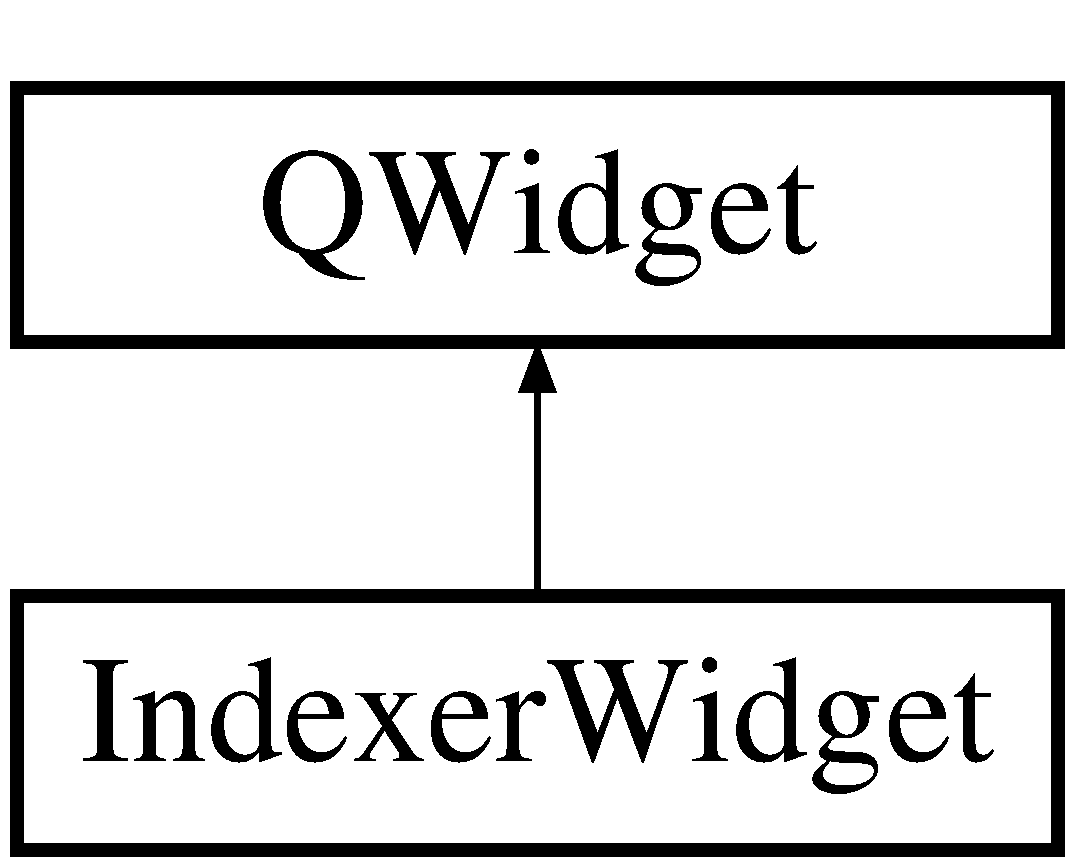
\includegraphics[height=2.000000cm]{classIndexerWidget}
\end{center}
\end{figure}
\subsubsection*{Public Slots}
\begin{DoxyCompactItemize}
\item 
void \mbox{\hyperlink{classIndexerWidget_aebacace6caa148439e640d27b6142e5e}{print\+Finish}} ()
\item 
void \mbox{\hyperlink{classIndexerWidget_ac3c769e1ba1434dcbebb4b2b4bdc79e4}{print\+Start}} ()
\item 
void \mbox{\hyperlink{classIndexerWidget_a80cbb27852773541d0fe05d44b571f20}{set\+State}} (u\+\_\+int16\+\_\+t state)
\item 
void \mbox{\hyperlink{classIndexerWidget_a198605c5b4c5f008b0baef3b19b0cdea}{reset\+Widget}} ()
\end{DoxyCompactItemize}
\subsubsection*{Signals}
\begin{DoxyCompactItemize}
\item 
void \mbox{\hyperlink{classIndexerWidget_a5b786596789da83ff37ad1c8df223d0f}{setting\+Button\+Cliced}} ()
\item 
void \mbox{\hyperlink{classIndexerWidget_ae1a3d974cf2f93385e76e635df2a4c07}{send\+Command}} (Q\+Byte\+Array command)
\item 
void \mbox{\hyperlink{classIndexerWidget_aa88ef42bb8acd6b90405d7e38784d7af}{reset\+Request}} ()
\item 
void \mbox{\hyperlink{classIndexerWidget_a31cbe782d1f10a27c6f80924c8445ae5}{start\+Print}} (bool is\+Auto)
\item 
void \mbox{\hyperlink{classIndexerWidget_a1fff5da56d91020863b52f17a4dc6f49}{stop\+Print}} ()
\end{DoxyCompactItemize}
\subsubsection*{Public Member Functions}
\begin{DoxyCompactItemize}
\item 
\mbox{\hyperlink{classIndexerWidget_a5406b617d20c983f0208d78813f46b13}{Indexer\+Widget}} (Q\+Widget $\ast$parent=0)
\item 
\mbox{\hyperlink{classIndexerWidget_a06e073bb57ddfdbfc21364f8344e10f3}{$\sim$\+Indexer\+Widget}} ()
\item 
bool \mbox{\hyperlink{classIndexerWidget_a7e4a847aba65f7a17c5b6ceaf8a59636}{get\+Is\+Auto\+Print}} ()
\item 
void \mbox{\hyperlink{classIndexerWidget_af3faa0bf1c820ff960f0f4be49ed453b}{set\+Icon\+Folder}} (Q\+String path)
\item 
void \mbox{\hyperlink{classIndexerWidget_abe1eb2eae0c93dff7d5f0d9cbf9cd371}{click\+Button}} (Q\+Byte\+Array data)
\end{DoxyCompactItemize}
\subsubsection*{Protected Member Functions}
\begin{DoxyCompactItemize}
\item 
virtual void \mbox{\hyperlink{classIndexerWidget_a60d4e0e97023327226e6390e9b867fc8}{resize\+Event}} (Q\+Resize\+Event $\ast$e)
\item 
void \mbox{\hyperlink{classIndexerWidget_a6c63cfdeb49de1b9a64a6b3fc8b4d997}{change\+Event}} (Q\+Event $\ast$event)
\end{DoxyCompactItemize}
\subsubsection*{Private Slots}
\begin{DoxyCompactItemize}
\item 
void \mbox{\hyperlink{classIndexerWidget_a5700a9df0a8d83253d5b4c1a7908a3f0}{on\+\_\+p\+Button\+Lock\+\_\+clicked}} ()
\item 
void \mbox{\hyperlink{classIndexerWidget_ace858fa20587dd1cf2822b278f8baf95}{on\+\_\+p\+Button\+Move\+\_\+clicked}} ()
\item 
void \mbox{\hyperlink{classIndexerWidget_a32ceafc2476b8822b1865a39ea5f4aa3}{on\+\_\+p\+Button\+Auto\+\_\+clicked}} ()
\item 
void \mbox{\hyperlink{classIndexerWidget_a556d0a3c344dc91460458f8958423991}{on\+\_\+p\+Button\+Print\+\_\+clicked}} ()
\item 
void \mbox{\hyperlink{classIndexerWidget_ab6e2ace22ecd642d1090c103467d51fa}{on\+\_\+p\+Button\+Move\+Left\+\_\+clicked}} ()
\item 
void \mbox{\hyperlink{classIndexerWidget_a5391681e2ddcad15da823c41f21974fc}{on\+\_\+p\+Button\+Move\+Up\+\_\+clicked}} ()
\item 
void \mbox{\hyperlink{classIndexerWidget_a9b3217e574ec1791e91a38c6ddddad35}{on\+\_\+p\+Button\+Move\+Right\+\_\+clicked}} ()
\item 
void \mbox{\hyperlink{classIndexerWidget_ac4ccc271795ea968fa3c2c173ac2898e}{on\+\_\+p\+Button\+Reset\+\_\+clicked}} ()
\item 
void \mbox{\hyperlink{classIndexerWidget_a4d375a44ccc6c5d096667940e5e6fe10}{on\+\_\+p\+Button\+Home\+\_\+clicked}} ()
\item 
void \mbox{\hyperlink{classIndexerWidget_a4621d1eb9163b44c7d5343551e8bb225}{setting\+P\+Button\+Clic\+Slot}} ()
\item 
void \mbox{\hyperlink{classIndexerWidget_a5c46c6c40102a7f753028a0b4d5ae57c}{on\+\_\+p\+Button\+Air\+\_\+clicked}} ()
\end{DoxyCompactItemize}
\subsubsection*{Private Attributes}
\begin{DoxyCompactItemize}
\item 
Ui\+::\+Indexer\+Widget $\ast$ \mbox{\hyperlink{classIndexerWidget_acfec1850dc331214abc0eb65093a5896}{ui}}
\item 
Q\+Push\+Button $\ast$ \mbox{\hyperlink{classIndexerWidget_a9f5ddd2008811969c702188992f1a3da}{p\+Button\+Sets}}
\item 
int \mbox{\hyperlink{classIndexerWidget_a113ecc934dd986f975553c6a55d05523}{half\+Counter}}
\item 
bool \mbox{\hyperlink{classIndexerWidget_a7d299b2455b965aad9652489b957b618}{is\+Auto\+Print\+Enable}}
\item 
Q\+String \mbox{\hyperlink{classIndexerWidget_ad3787e740fc417fdcb74202c9953788f}{path\+Icon}}
\item 
\mbox{\hyperlink{classMachineSettings_a3d02f0565ba9c53dbb59d5d086208cad}{Machine\+Settings\+::\+Machine\+State}} \mbox{\hyperlink{classIndexerWidget_ad0cd90b88ff25e18b46f5af290c9dcae}{machine\+State}}
\end{DoxyCompactItemize}


\subsubsection{Constructor \& Destructor Documentation}
\mbox{\Hypertarget{classIndexerWidget_a5406b617d20c983f0208d78813f46b13}\label{classIndexerWidget_a5406b617d20c983f0208d78813f46b13}} 
\index{Indexer\+Widget@{Indexer\+Widget}!Indexer\+Widget@{Indexer\+Widget}}
\index{Indexer\+Widget@{Indexer\+Widget}!Indexer\+Widget@{Indexer\+Widget}}
{\footnotesize\ttfamily Indexer\+Widget\+::\texorpdfstring{Indexer\+Widget()}{IndexerWidget()} (\begin{DoxyParamCaption}\item[{Q\+Widget $\ast$}]{parent = {\ttfamily 0} }\end{DoxyParamCaption}){\ttfamily [explicit]}} - standard Q\+Widget constructor. In constructor initialized  \hyperlink{classIndexerWidget_a9f5ddd2008811969c702188992f1a3da}{p\+Button\+Sets}, resize it and move it to it's place.

\mbox{\Hypertarget{classIndexerWidget_a06e073bb57ddfdbfc21364f8344e10f3}\label{classIndexerWidget_a06e073bb57ddfdbfc21364f8344e10f3}} 
\index{Indexer\+Widget@{Indexer\+Widget}!````~Indexer\+Widget@{$\sim$\+Indexer\+Widget}}
\index{````~Indexer\+Widget@{$\sim$\+Indexer\+Widget}!Indexer\+Widget@{Indexer\+Widget}}
{\footnotesize\ttfamily Indexer\+Widget\+::\texorpdfstring{$\sim$\+Indexer\+Widget()}{~IndexerWidget()} (\begin{DoxyParamCaption}{ }\end{DoxyParamCaption})} - standard Q\+Widget destructor.

\subsubsection{Member Function Documentation}
\mbox{\Hypertarget{classIndexerWidget_a6c63cfdeb49de1b9a64a6b3fc8b4d997}\label{classIndexerWidget_a6c63cfdeb49de1b9a64a6b3fc8b4d997}} 
\index{Indexer\+Widget@{Indexer\+Widget}!change\+Event@{change\+Event}}
\index{change\+Event@{change\+Event}!Indexer\+Widget@{Indexer\+Widget}}
{\footnotesize\ttfamily void Indexer\+Widget\+::\texorpdfstring{change\+Event}{changeEvent} (\begin{DoxyParamCaption}\item[{Q\+Event $\ast$}]{event }\end{DoxyParamCaption}){\ttfamily [protected]}} - Reimplementation of default event for Q\+Widget to enable user interface translation. Function called automatically.

\mbox{\Hypertarget{classIndexerWidget_abe1eb2eae0c93dff7d5f0d9cbf9cd371}\label{classIndexerWidget_abe1eb2eae0c93dff7d5f0d9cbf9cd371}} 
\index{Indexer\+Widget@{Indexer\+Widget}!click\+Button@{click\+Button}}
\index{click\+Button@{click\+Button}!Indexer\+Widget@{Indexer\+Widget}}
{\footnotesize\ttfamily void Indexer\+Widget\+::\texorpdfstring{click\+Button}{clickButton} (\begin{DoxyParamCaption}\item[{Q\+Byte\+Array}]{data }\end{DoxyParamCaption})} - function to imitate clicking of button. Which button will be clicked is selecting by contents of \textit{data}.

\mbox{\Hypertarget{classIndexerWidget_a7e4a847aba65f7a17c5b6ceaf8a59636}\label{classIndexerWidget_a7e4a847aba65f7a17c5b6ceaf8a59636}} 
\index{Indexer\+Widget@{Indexer\+Widget}!get\+Is\+Auto\+Print@{get\+Is\+Auto\+Print}}
\index{get\+Is\+Auto\+Print@{get\+Is\+Auto\+Print}!Indexer\+Widget@{Indexer\+Widget}}
{\footnotesize\ttfamily bool Indexer\+Widget\+::\texorpdfstring{get\+Is\+Auto\+Print}{getIsAutoPrint} (\begin{DoxyParamCaption}{ }\end{DoxyParamCaption})} - return state of p\+Button\+Auto. Used in parent object.

	\begin{center}	\line(1,0){450} \end{center}
Functions in next block used to send commands to master PCB to control machine. Data in package tacked from \hyperlink{classIndexerLiftSettings_ad0959473f792741cadaa262730f5a463}{Indexer\+Commands\+En} enumerator. Method of commands data packing described in \hyperlink{classRegister}{Register} class reference. \\
\begin{DoxyCompactItemize}
\item\mbox{\Hypertarget{classIndexerWidget_a5c46c6c40102a7f753028a0b4d5ae57c}\label{classIndexerWidget_a5c46c6c40102a7f753028a0b4d5ae57c}} 
\index{Indexer\+Widget@{Indexer\+Widget}!on\+\_\+p\+Button\+Air\+\_\+clicked@{on\+\_\+p\+Button\+Air\+\_\+clicked}}
\index{on\+\_\+p\+Button\+Air\+\_\+clicked@{on\+\_\+p\+Button\+Air\+\_\+clicked}!Indexer\+Widget@{Indexer\+Widget}}
{\footnotesize\ttfamily void Indexer\+Widget\+::\texorpdfstring{on\+\_\+p\+Button\+Air\+\_\+clicked}{on\_pButtonAir\_clicked} (\begin{DoxyParamCaption}{ }\end{DoxyParamCaption}){\ttfamily [private]}, {\ttfamily [slot]}} - 

\item\mbox{\Hypertarget{classIndexerWidget_a32ceafc2476b8822b1865a39ea5f4aa3}\label{classIndexerWidget_a32ceafc2476b8822b1865a39ea5f4aa3}} 
\index{Indexer\+Widget@{Indexer\+Widget}!on\+\_\+p\+Button\+Auto\+\_\+clicked@{on\+\_\+p\+Button\+Auto\+\_\+clicked}}
\index{on\+\_\+p\+Button\+Auto\+\_\+clicked@{on\+\_\+p\+Button\+Auto\+\_\+clicked}!Indexer\+Widget@{Indexer\+Widget}}
{\footnotesize\ttfamily void Indexer\+Widget\+::\texorpdfstring{on\+\_\+p\+Button\+Auto\+\_\+clicked}{on\_pButtonAuto\_clicked} (\begin{DoxyParamCaption}{ }\end{DoxyParamCaption}){\ttfamily [private]}, {\ttfamily [slot]}}

\item\mbox{\Hypertarget{classIndexerWidget_a4d375a44ccc6c5d096667940e5e6fe10}\label{classIndexerWidget_a4d375a44ccc6c5d096667940e5e6fe10}} 
\index{Indexer\+Widget@{Indexer\+Widget}!on\+\_\+p\+Button\+Home\+\_\+clicked@{on\+\_\+p\+Button\+Home\+\_\+clicked}}
\index{on\+\_\+p\+Button\+Home\+\_\+clicked@{on\+\_\+p\+Button\+Home\+\_\+clicked}!Indexer\+Widget@{Indexer\+Widget}}
{\footnotesize\ttfamily void Indexer\+Widget\+::\texorpdfstring{on\+\_\+p\+Button\+Home\+\_\+clicked}{on\_pButtonHome\_clicked} (\begin{DoxyParamCaption}{ }\end{DoxyParamCaption}){\ttfamily [private]}, {\ttfamily [slot]}}

\item\mbox{\Hypertarget{classIndexerWidget_a5700a9df0a8d83253d5b4c1a7908a3f0}\label{classIndexerWidget_a5700a9df0a8d83253d5b4c1a7908a3f0}} 
\index{Indexer\+Widget@{Indexer\+Widget}!on\+\_\+p\+Button\+Lock\+\_\+clicked@{on\+\_\+p\+Button\+Lock\+\_\+clicked}}
\index{on\+\_\+p\+Button\+Lock\+\_\+clicked@{on\+\_\+p\+Button\+Lock\+\_\+clicked}!Indexer\+Widget@{Indexer\+Widget}}
{\footnotesize\ttfamily void Indexer\+Widget\+::\texorpdfstring{on\+\_\+p\+Button\+Lock\+\_\+clicked}{on\_pButtonLock\_clicked} (\begin{DoxyParamCaption}{ }\end{DoxyParamCaption}){\ttfamily [private]}, {\ttfamily [slot]}}

\item\mbox{\Hypertarget{classIndexerWidget_ace858fa20587dd1cf2822b278f8baf95}\label{classIndexerWidget_ace858fa20587dd1cf2822b278f8baf95}} 
\index{Indexer\+Widget@{Indexer\+Widget}!on\+\_\+p\+Button\+Move\+\_\+clicked@{on\+\_\+p\+Button\+Move\+\_\+clicked}}
\index{on\+\_\+p\+Button\+Move\+\_\+clicked@{on\+\_\+p\+Button\+Move\+\_\+clicked}!Indexer\+Widget@{Indexer\+Widget}}
{\footnotesize\ttfamily void Indexer\+Widget\+::\texorpdfstring{on\+\_\+p\+Button\+Move\+\_\+clicked}{on\_pButtonMove\_clicked} (\begin{DoxyParamCaption}{ }\end{DoxyParamCaption}){\ttfamily [private]}, {\ttfamily [slot]}}

\item\mbox{\Hypertarget{classIndexerWidget_ab6e2ace22ecd642d1090c103467d51fa}\label{classIndexerWidget_ab6e2ace22ecd642d1090c103467d51fa}} 
\index{Indexer\+Widget@{Indexer\+Widget}!on\+\_\+p\+Button\+Move\+Left\+\_\+clicked@{on\+\_\+p\+Button\+Move\+Left\+\_\+clicked}}
\index{on\+\_\+p\+Button\+Move\+Left\+\_\+clicked@{on\+\_\+p\+Button\+Move\+Left\+\_\+clicked}!Indexer\+Widget@{Indexer\+Widget}}
{\footnotesize\ttfamily void Indexer\+Widget\+::\texorpdfstring{on\+\_\+p\+Button\+Move\+Left\+\_\+clicked}{on\_pButtonMoveLeft\_clicked} (\begin{DoxyParamCaption}{ }\end{DoxyParamCaption}){\ttfamily [private]}, {\ttfamily [slot]}}

\item\mbox{\Hypertarget{classIndexerWidget_a9b3217e574ec1791e91a38c6ddddad35}\label{classIndexerWidget_a9b3217e574ec1791e91a38c6ddddad35}} 
\index{Indexer\+Widget@{Indexer\+Widget}!on\+\_\+p\+Button\+Move\+Right\+\_\+clicked@{on\+\_\+p\+Button\+Move\+Right\+\_\+clicked}}
\index{on\+\_\+p\+Button\+Move\+Right\+\_\+clicked@{on\+\_\+p\+Button\+Move\+Right\+\_\+clicked}!Indexer\+Widget@{Indexer\+Widget}}
{\footnotesize\ttfamily void Indexer\+Widget\+::\texorpdfstring{on\+\_\+p\+Button\+Move\+Right\+\_\+clicked}{on\_pButtonMoveRight\_clicked} (\begin{DoxyParamCaption}{ }\end{DoxyParamCaption}){\ttfamily [private]}, {\ttfamily [slot]}}

\item\mbox{\Hypertarget{classIndexerWidget_a5391681e2ddcad15da823c41f21974fc}\label{classIndexerWidget_a5391681e2ddcad15da823c41f21974fc}} 
\index{Indexer\+Widget@{Indexer\+Widget}!on\+\_\+p\+Button\+Move\+Up\+\_\+clicked@{on\+\_\+p\+Button\+Move\+Up\+\_\+clicked}}
\index{on\+\_\+p\+Button\+Move\+Up\+\_\+clicked@{on\+\_\+p\+Button\+Move\+Up\+\_\+clicked}!Indexer\+Widget@{Indexer\+Widget}}
{\footnotesize\ttfamily void Indexer\+Widget\+::\texorpdfstring{on\+\_\+p\+Button\+Move\+Up\+\_\+clicked}{on\_pButtonMoveUp\_clicked} (\begin{DoxyParamCaption}{ }\end{DoxyParamCaption}){\ttfamily [private]}, {\ttfamily [slot]}}

\item\mbox{\Hypertarget{classIndexerWidget_a556d0a3c344dc91460458f8958423991}\label{classIndexerWidget_a556d0a3c344dc91460458f8958423991}} 
\index{Indexer\+Widget@{Indexer\+Widget}!on\+\_\+p\+Button\+Print\+\_\+clicked@{on\+\_\+p\+Button\+Print\+\_\+clicked}}
\index{on\+\_\+p\+Button\+Print\+\_\+clicked@{on\+\_\+p\+Button\+Print\+\_\+clicked}!Indexer\+Widget@{Indexer\+Widget}}
{\footnotesize\ttfamily void Indexer\+Widget\+::\texorpdfstring{on\+\_\+p\+Button\+Print\+\_\+clicked}{on\_pButtonPrint\_clicked} (\begin{DoxyParamCaption}{ }\end{DoxyParamCaption}){\ttfamily [private]}, {\ttfamily [slot]}}

\item\mbox{\Hypertarget{classIndexerWidget_ac4ccc271795ea968fa3c2c173ac2898e}\label{classIndexerWidget_ac4ccc271795ea968fa3c2c173ac2898e}} 
\index{Indexer\+Widget@{Indexer\+Widget}!on\+\_\+p\+Button\+Reset\+\_\+clicked@{on\+\_\+p\+Button\+Reset\+\_\+clicked}}
\index{on\+\_\+p\+Button\+Reset\+\_\+clicked@{on\+\_\+p\+Button\+Reset\+\_\+clicked}!Indexer\+Widget@{Indexer\+Widget}}
{\footnotesize\ttfamily void Indexer\+Widget\+::\texorpdfstring{on\+\_\+p\+Button\+Reset\+\_\+clicked}{on\_pButtonReset\_clicked} (\begin{DoxyParamCaption}{ }\end{DoxyParamCaption}){\ttfamily [private]}, {\ttfamily [slot]}}
\end{DoxyCompactItemize}
	\begin{center}	\line(1,0){450} \end{center}
	
\mbox{\Hypertarget{classIndexerWidget_aebacace6caa148439e640d27b6142e5e}\label{classIndexerWidget_aebacace6caa148439e640d27b6142e5e}} 
\index{Indexer\+Widget@{Indexer\+Widget}!print\+Finish@{print\+Finish}}
\index{print\+Finish@{print\+Finish}!Indexer\+Widget@{Indexer\+Widget}}
{\footnotesize\ttfamily void Indexer\+Widget\+::\texorpdfstring{print\+Finish}{printFinish} (\begin{DoxyParamCaption}{ }\end{DoxyParamCaption}){\ttfamily [slot]}} - unused function.

\mbox{\Hypertarget{classIndexerWidget_ac3c769e1ba1434dcbebb4b2b4bdc79e4}\label{classIndexerWidget_ac3c769e1ba1434dcbebb4b2b4bdc79e4}} 
\index{Indexer\+Widget@{Indexer\+Widget}!print\+Start@{print\+Start}}
\index{print\+Start@{print\+Start}!Indexer\+Widget@{Indexer\+Widget}}
{\footnotesize\ttfamily void Indexer\+Widget\+::\texorpdfstring{print\+Start}{printStart} (\begin{DoxyParamCaption}{ }\end{DoxyParamCaption}){\ttfamily [slot]}} - unused function.

\mbox{\Hypertarget{classIndexerWidget_aa88ef42bb8acd6b90405d7e38784d7af}\label{classIndexerWidget_aa88ef42bb8acd6b90405d7e38784d7af}} 
\index{Indexer\+Widget@{Indexer\+Widget}!reset\+Request@{reset\+Request}}
\index{reset\+Request@{reset\+Request}!Indexer\+Widget@{Indexer\+Widget}}
{\footnotesize\ttfamily void Indexer\+Widget\+::\texorpdfstring{reset\+Request}{resetRequest} (\begin{DoxyParamCaption}{ }\end{DoxyParamCaption}){\ttfamily [signal]}} - signal which emit by \hyperlink{classIndexerWidget_ac4ccc271795ea968fa3c2c173ac2898e}{on\+\_\+p\+Button\+Reset\+\_\+clicked}(...) function and handle in parent object by \hyperlink{classMainWindow_a2d957a5c154ebce97484e8aa7fa2abb3}{reset\+Machine}(...) function.

\mbox{\Hypertarget{classIndexerWidget_a198605c5b4c5f008b0baef3b19b0cdea}\label{classIndexerWidget_a198605c5b4c5f008b0baef3b19b0cdea}} 
\index{Indexer\+Widget@{Indexer\+Widget}!reset\+Widget@{reset\+Widget}}
\index{reset\+Widget@{reset\+Widget}!Indexer\+Widget@{Indexer\+Widget}}
{\footnotesize\ttfamily void Indexer\+Widget\+::\texorpdfstring{reset\+Widget}{resetWidget} (\begin{DoxyParamCaption}{ }\end{DoxyParamCaption}){\ttfamily [slot]}} - function to return buttons on widget to initial state.

\mbox{\Hypertarget{classIndexerWidget_a60d4e0e97023327226e6390e9b867fc8}\label{classIndexerWidget_a60d4e0e97023327226e6390e9b867fc8}} 
\index{Indexer\+Widget@{Indexer\+Widget}!resize\+Event@{resize\+Event}}
\index{resize\+Event@{resize\+Event}!Indexer\+Widget@{Indexer\+Widget}}
{\footnotesize\ttfamily void Indexer\+Widget\+::\texorpdfstring{resize\+Event()}{resizeEvent()} (\begin{DoxyParamCaption}\item[{Q\+Resize\+Event $\ast$}]{e }\end{DoxyParamCaption}){\ttfamily [protected]}, {\ttfamily [virtual]}} - reimplementation of standard function to move setting button to new place after widget resize. Function call automatically. 

\mbox{\Hypertarget{classIndexerWidget_ae1a3d974cf2f93385e76e635df2a4c07}\label{classIndexerWidget_ae1a3d974cf2f93385e76e635df2a4c07}} 
\index{Indexer\+Widget@{Indexer\+Widget}!send\+Command@{send\+Command}}
\index{send\+Command@{send\+Command}!Indexer\+Widget@{Indexer\+Widget}}
{\footnotesize\ttfamily void Indexer\+Widget\+::\texorpdfstring{send\+Command}{sendCommand} (\begin{DoxyParamCaption}\item[{Q\+Byte\+Array}]{command }\end{DoxyParamCaption}){\ttfamily [signal]}}- signal to send data in Q\+Byte\+Array format to handle in parent object and send it to serial port.

\mbox{\Hypertarget{classIndexerWidget_af3faa0bf1c820ff960f0f4be49ed453b}\label{classIndexerWidget_af3faa0bf1c820ff960f0f4be49ed453b}} 
\index{Indexer\+Widget@{Indexer\+Widget}!set\+Icon\+Folder@{set\+Icon\+Folder}}
\index{set\+Icon\+Folder@{set\+Icon\+Folder}!Indexer\+Widget@{Indexer\+Widget}}
{\footnotesize\ttfamily void Indexer\+Widget\+::\texorpdfstring{set\+Icon\+Folder}{setIconFolder} (\begin{DoxyParamCaption}\item[{Q\+String}]{path }\end{DoxyParamCaption})}- function to change folder with icons which used on view and update icons. Icon path written to \hyperlink{classIndexerWidget_ad3787e740fc417fdcb74202c9953788f}{path\+Icon} variable.

\mbox{\Hypertarget{classIndexerWidget_a80cbb27852773541d0fe05d44b571f20}\label{classIndexerWidget_a80cbb27852773541d0fe05d44b571f20}} 
\index{Indexer\+Widget@{Indexer\+Widget}!set\+State@{set\+State}}
\index{set\+State@{set\+State}!Indexer\+Widget@{Indexer\+Widget}}
{\footnotesize\ttfamily void Indexer\+Widget\+::\texorpdfstring{set\+State}{setState} (\begin{DoxyParamCaption}\item[{u\+\_\+int16\+\_\+t}]{state }\end{DoxyParamCaption}){\ttfamily [slot]}} - function to set state of widget. State describe which buttons will be enabled or disabled, visible or hidden. State of widget sets by master board of machine, when \hyperlink{structRegister_1_1MasterReg___1_1reg}{Register\+::\+Master\+Reg\+\_\+\+::reg} field \hyperlink{structRegister_1_1MasterReg___1_1reg_aa5111a7f8eddbd8f8d6c92e23f326946}{master\+Reg\+\_\+\+E\+KR} updates its value.

\mbox{\Hypertarget{classIndexerWidget_a5b786596789da83ff37ad1c8df223d0f}\label{classIndexerWidget_a5b786596789da83ff37ad1c8df223d0f}} 
\index{Indexer\+Widget@{Indexer\+Widget}!setting\+Button\+Cliced@{setting\+Button\+Cliced}}
\index{setting\+Button\+Cliced@{setting\+Button\+Cliced}!Indexer\+Widget@{Indexer\+Widget}}
{\footnotesize\ttfamily void Indexer\+Widget\+::\texorpdfstring{setting\+Button\+Cliced}{settingButtonCliced} (\begin{DoxyParamCaption}{ }\end{DoxyParamCaption}){\ttfamily [signal]}} - signal which emitted by \hyperlink{classIndexerWidget_a4621d1eb9163b44c7d5343551e8bb225}{setting\+P\+Button\+Clic\+Slot}(...) function and handle in parent object by \hyperlink{classMainWindow_a867f15b0c134336e5477e80673f1903d}{indexer\+Lift\+Setting\+Request}(...) function.

\mbox{\Hypertarget{classIndexerWidget_a4621d1eb9163b44c7d5343551e8bb225}\label{classIndexerWidget_a4621d1eb9163b44c7d5343551e8bb225}} 
\index{Indexer\+Widget@{Indexer\+Widget}!setting\+P\+Button\+Clic\+Slot@{setting\+P\+Button\+Clic\+Slot}}
\index{setting\+P\+Button\+Clic\+Slot@{setting\+P\+Button\+Clic\+Slot}!Indexer\+Widget@{Indexer\+Widget}}
{\footnotesize\ttfamily void Indexer\+Widget\+::\texorpdfstring{setting\+P\+Button\+Clic\+Slot}{settingPButtonClicSlot} (\begin{DoxyParamCaption}{ }\end{DoxyParamCaption}){\ttfamily [private]}, {\ttfamily [slot]}} - function which called by \hyperlink{classIndexerWidget_a9f5ddd2008811969c702188992f1a3da}{p\+Button\+Sets} click signal and emit {\hyperlink{classIndexerWidget_a5b786596789da83ff37ad1c8df223d0f}{setting\+Button\+Cliced}(...) signal.

\mbox{\Hypertarget{classIndexerWidget_a31cbe782d1f10a27c6f80924c8445ae5}\label{classIndexerWidget_a31cbe782d1f10a27c6f80924c8445ae5}} 
\index{Indexer\+Widget@{Indexer\+Widget}!start\+Print@{start\+Print}}
\index{start\+Print@{start\+Print}!Indexer\+Widget@{Indexer\+Widget}}
{\footnotesize\ttfamily void Indexer\+Widget\+::\texorpdfstring{start\+Print}{startPrint} (\begin{DoxyParamCaption}\item[{bool}]{is\+Auto }\end{DoxyParamCaption}){\ttfamily [signal]}} - signal which handle in parent object by \hyperlink{classMainWindow_a18d83d170a660644bb70fda6b28a2bc6}{start\+Print\+Process}(...) function.

\mbox{\Hypertarget{classIndexerWidget_a1fff5da56d91020863b52f17a4dc6f49}\label{classIndexerWidget_a1fff5da56d91020863b52f17a4dc6f49}} 
\index{Indexer\+Widget@{Indexer\+Widget}!stop\+Print@{stop\+Print}}
\index{stop\+Print@{stop\+Print}!Indexer\+Widget@{Indexer\+Widget}}
{\footnotesize\ttfamily void Indexer\+Widget\+::\texorpdfstring{stop\+Print}{stopPrint} (\begin{DoxyParamCaption}{ }\end{DoxyParamCaption}){\ttfamily [signal]}} - signal which handle in parent object by \hyperlink{classMainWindow_a80282fbc6eb85c0f6594975e02a150a3}{stop\+Print\+Process}(...) function.



\subsubsection{Member Data Documentation}
\mbox{\Hypertarget{classIndexerWidget_a113ecc934dd986f975553c6a55d05523}\label{classIndexerWidget_a113ecc934dd986f975553c6a55d05523}} 
\index{Indexer\+Widget@{Indexer\+Widget}!half\+Counter@{half\+Counter}}
\index{half\+Counter@{half\+Counter}!Indexer\+Widget@{Indexer\+Widget}}
{\footnotesize\ttfamily int Indexer\+Widget\+::\texorpdfstring{half\+Counter}{halfCounter}{\ttfamily [private]}} - variable which contain count of steps in half mode to hide/\+show p\+Button\+Move.

\mbox{\Hypertarget{classIndexerWidget_a7d299b2455b965aad9652489b957b618}\label{classIndexerWidget_a7d299b2455b965aad9652489b957b618}} 
\index{Indexer\+Widget@{Indexer\+Widget}!is\+Auto\+Print\+Enable@{is\+Auto\+Print\+Enable}}
\index{is\+Auto\+Print\+Enable@{is\+Auto\+Print\+Enable}!Indexer\+Widget@{Indexer\+Widget}}
{\footnotesize\ttfamily bool Indexer\+Widget\+::\texorpdfstring{is\+Auto\+Print\+Enable}{isAutoPrintEnable}{\ttfamily [private]}}

\mbox{\Hypertarget{classIndexerWidget_ad0cd90b88ff25e18b46f5af290c9dcae}\label{classIndexerWidget_ad0cd90b88ff25e18b46f5af290c9dcae}} 
\index{Indexer\+Widget@{Indexer\+Widget}!machine\+State@{machine\+State}}
\index{machine\+State@{machine\+State}!Indexer\+Widget@{Indexer\+Widget}}
{\footnotesize\ttfamily \mbox{\hyperlink{classMachineSettings_a3d02f0565ba9c53dbb59d5d086208cad}{Machine\+Settings\+::\+Machine\+State}} Indexer\+Widget\+::\texorpdfstring{machine\+State}{machineState}{\ttfamily [private]}} - variable to contain state of machine. 

\mbox{\Hypertarget{classIndexerWidget_ad3787e740fc417fdcb74202c9953788f}\label{classIndexerWidget_ad3787e740fc417fdcb74202c9953788f}} 
\index{Indexer\+Widget@{Indexer\+Widget}!path\+Icon@{path\+Icon}}
\index{path\+Icon@{path\+Icon}!Indexer\+Widget@{Indexer\+Widget}}
{\footnotesize\ttfamily Q\+String Indexer\+Widget\+::\texorpdfstring{path\+Icon}{pathIcon}{\ttfamily [private]}} - variable to contain path to icon folder.

\mbox{\Hypertarget{classIndexerWidget_a9f5ddd2008811969c702188992f1a3da}\label{classIndexerWidget_a9f5ddd2008811969c702188992f1a3da}} 
\index{Indexer\+Widget@{Indexer\+Widget}!p\+Button\+Sets@{p\+Button\+Sets}}
\index{p\+Button\+Sets@{p\+Button\+Sets}!Indexer\+Widget@{Indexer\+Widget}}
{\footnotesize\ttfamily Q\+Push\+Button$\ast$ Indexer\+Widget\+::\texorpdfstring{p\+Button\+Sets}{pButtonSets}{\ttfamily [private]}} - Q\+Push\+Button class object.


The documentation for this class was generated from the following files\+:\begin{DoxyCompactItemize}
\item 
\mbox{\hyperlink{indexerwidget_8h}{indexerwidget.\+h}}\item 
\mbox{\hyperlink{indexerwidget_8cpp}{indexerwidget.\+cpp}}\end{DoxyCompactItemize}
\newpage
\hypertarget{structIndexerLiftSettings_1_1IndexParameters__}{}\subsection{Indexer\+Lift\+Settings\+:\+:Index\+Parameters\+\_\+ Struct Reference}
\label{structIndexerLiftSettings_1_1IndexParameters__}\index{Indexer\+Lift\+Settings\+::\+Index\+Parameters\+\_\+@{Indexer\+Lift\+Settings\+::\+Index\+Parameters\+\_\+}}


{\ttfamily \#include $<$settings.\+h$>$}

\subsubsection*{Public Member Functions}
\begin{DoxyCompactItemize}
\item 
Q\+Byte\+Array \mbox{\hyperlink{structIndexerLiftSettings_1_1IndexParameters___a2ed5d38af73aae6fe65d2e0d928eb42a}{to\+Byte\+Array}} ()
\end{DoxyCompactItemize}
\subsubsection*{Public Attributes}
\begin{DoxyCompactItemize}
\item 
\mbox{\hyperlink{settings_8h_a017dd44e68049ffdd31500a8cd01ba68}{uint16\+\_\+t}} \mbox{\hyperlink{structIndexerLiftSettings_1_1IndexParameters___acf98dbf8129022be81355dc1e4a70203}{distance}}
\item 
int16\+\_\+t \mbox{\hyperlink{structIndexerLiftSettings_1_1IndexParameters___ad9ab7cc5780480b481d54e03102e5f79}{home\+Offset}}
\item 
int16\+\_\+t \mbox{\hyperlink{structIndexerLiftSettings_1_1IndexParameters___adfe603b56a3ef4624bb59390a08c19cf}{dist\+Offcet}}
\item 
\mbox{\hyperlink{settings_8h_a017dd44e68049ffdd31500a8cd01ba68}{uint16\+\_\+t}} \mbox{\hyperlink{structIndexerLiftSettings_1_1IndexParameters___a7cff4645b11fbdf47e73e7faadf8bc9f}{speed}}
\item 
\mbox{\hyperlink{settings_8h_a017dd44e68049ffdd31500a8cd01ba68}{uint16\+\_\+t}} \mbox{\hyperlink{structIndexerLiftSettings_1_1IndexParameters___adb7016a7d40f054ae4d534e6d7a3ad9e}{acceleration}}
\item 
\mbox{\hyperlink{settings_8h_a017dd44e68049ffdd31500a8cd01ba68}{uint16\+\_\+t}} \mbox{\hyperlink{structIndexerLiftSettings_1_1IndexParameters___af2b7b9756b272b7b60023be484749dad}{speed\+Ret}}
\item 
\mbox{\hyperlink{settings_8h_a017dd44e68049ffdd31500a8cd01ba68}{uint16\+\_\+t}} \mbox{\hyperlink{structIndexerLiftSettings_1_1IndexParameters___a8a602a3ffc41e9ab7d7979a260110427}{acceleration\+Ret}}
\end{DoxyCompactItemize}


\subsubsection{Member Function Documentation}
\mbox{\Hypertarget{structIndexerLiftSettings_1_1IndexParameters___a2ed5d38af73aae6fe65d2e0d928eb42a}\label{structIndexerLiftSettings_1_1IndexParameters___a2ed5d38af73aae6fe65d2e0d928eb42a}} 
\index{Indexer\+Lift\+Settings\+::\+Index\+Parameters\+\_\+@{Indexer\+Lift\+Settings\+::\+Index\+Parameters\+\_\+}!to\+Byte\+Array@{to\+Byte\+Array}}
\index{to\+Byte\+Array@{to\+Byte\+Array}!Indexer\+Lift\+Settings\+::\+Index\+Parameters\+\_\+@{Indexer\+Lift\+Settings\+::\+Index\+Parameters\+\_\+}}
{\footnotesize\ttfamily Q\+Byte\+Array Indexer\+Lift\+Settings\+::\+Index\+Parameters\+\_\+\+::\texorpdfstring{to\+Byte\+Array}{toByteArray} (\begin{DoxyParamCaption}{ }\end{DoxyParamCaption})}- function to gather all structure items to Q\+Byte\+Array to have possibility save data on hard drive in compact format.



\subsubsection{Member Data Documentation}
\mbox{\Hypertarget{structIndexerLiftSettings_1_1IndexParameters___adb7016a7d40f054ae4d534e6d7a3ad9e}\label{structIndexerLiftSettings_1_1IndexParameters___adb7016a7d40f054ae4d534e6d7a3ad9e}} 
\index{Indexer\+Lift\+Settings\+::\+Index\+Parameters\+\_\+@{Indexer\+Lift\+Settings\+::\+Index\+Parameters\+\_\+}!acceleration@{acceleration}}
\index{acceleration@{acceleration}!Indexer\+Lift\+Settings\+::\+Index\+Parameters\+\_\+@{Indexer\+Lift\+Settings\+::\+Index\+Parameters\+\_\+}}
{\footnotesize\ttfamily \mbox{\hyperlink{settings_8h_a017dd44e68049ffdd31500a8cd01ba68}{uint16\+\_\+t}} Indexer\+Lift\+Settings\+::\+Index\+Parameters\+\_\+\+::\texorpdfstring{acceleration}{acceleration}}

\mbox{\Hypertarget{structIndexerLiftSettings_1_1IndexParameters___a8a602a3ffc41e9ab7d7979a260110427}\label{structIndexerLiftSettings_1_1IndexParameters___a8a602a3ffc41e9ab7d7979a260110427}} 
\index{Indexer\+Lift\+Settings\+::\+Index\+Parameters\+\_\+@{Indexer\+Lift\+Settings\+::\+Index\+Parameters\+\_\+}!acceleration\+Ret@{acceleration\+Ret}}
\index{acceleration\+Ret@{acceleration\+Ret}!Indexer\+Lift\+Settings\+::\+Index\+Parameters\+\_\+@{Indexer\+Lift\+Settings\+::\+Index\+Parameters\+\_\+}}
{\footnotesize\ttfamily \mbox{\hyperlink{settings_8h_a017dd44e68049ffdd31500a8cd01ba68}{uint16\+\_\+t}} Indexer\+Lift\+Settings\+::\+Index\+Parameters\+\_\+\+::\texorpdfstring{acceleration\+Ret}{accelerationRet}}

\mbox{\Hypertarget{structIndexerLiftSettings_1_1IndexParameters___acf98dbf8129022be81355dc1e4a70203}\label{structIndexerLiftSettings_1_1IndexParameters___acf98dbf8129022be81355dc1e4a70203}} 
\index{Indexer\+Lift\+Settings\+::\+Index\+Parameters\+\_\+@{Indexer\+Lift\+Settings\+::\+Index\+Parameters\+\_\+}!distance@{distance}}
\index{distance@{distance}!Indexer\+Lift\+Settings\+::\+Index\+Parameters\+\_\+@{Indexer\+Lift\+Settings\+::\+Index\+Parameters\+\_\+}}
{\footnotesize\ttfamily \mbox{\hyperlink{settings_8h_a017dd44e68049ffdd31500a8cd01ba68}{uint16\+\_\+t}} Indexer\+Lift\+Settings\+::\+Index\+Parameters\+\_\+\+::\texorpdfstring{distance}{distance}}

\mbox{\Hypertarget{structIndexerLiftSettings_1_1IndexParameters___adfe603b56a3ef4624bb59390a08c19cf}\label{structIndexerLiftSettings_1_1IndexParameters___adfe603b56a3ef4624bb59390a08c19cf}} 
\index{Indexer\+Lift\+Settings\+::\+Index\+Parameters\+\_\+@{Indexer\+Lift\+Settings\+::\+Index\+Parameters\+\_\+}!dist\+Offcet@{dist\+Offcet}}
\index{dist\+Offcet@{dist\+Offcet}!Indexer\+Lift\+Settings\+::\+Index\+Parameters\+\_\+@{Indexer\+Lift\+Settings\+::\+Index\+Parameters\+\_\+}}
{\footnotesize\ttfamily int16\+\_\+t Indexer\+Lift\+Settings\+::\+Index\+Parameters\+\_\+\+::\texorpdfstring{dist\+Offcet}{distOffcet}}

\mbox{\Hypertarget{structIndexerLiftSettings_1_1IndexParameters___ad9ab7cc5780480b481d54e03102e5f79}\label{structIndexerLiftSettings_1_1IndexParameters___ad9ab7cc5780480b481d54e03102e5f79}} 
\index{Indexer\+Lift\+Settings\+::\+Index\+Parameters\+\_\+@{Indexer\+Lift\+Settings\+::\+Index\+Parameters\+\_\+}!home\+Offset@{home\+Offset}}
\index{home\+Offset@{home\+Offset}!Indexer\+Lift\+Settings\+::\+Index\+Parameters\+\_\+@{Indexer\+Lift\+Settings\+::\+Index\+Parameters\+\_\+}}
{\footnotesize\ttfamily int16\+\_\+t Indexer\+Lift\+Settings\+::\+Index\+Parameters\+\_\+\+::\texorpdfstring{home\+Offset}{homeOffset}}

\mbox{\Hypertarget{structIndexerLiftSettings_1_1IndexParameters___a7cff4645b11fbdf47e73e7faadf8bc9f}\label{structIndexerLiftSettings_1_1IndexParameters___a7cff4645b11fbdf47e73e7faadf8bc9f}} 
\index{Indexer\+Lift\+Settings\+::\+Index\+Parameters\+\_\+@{Indexer\+Lift\+Settings\+::\+Index\+Parameters\+\_\+}!speed@{speed}}
\index{speed@{speed}!Indexer\+Lift\+Settings\+::\+Index\+Parameters\+\_\+@{Indexer\+Lift\+Settings\+::\+Index\+Parameters\+\_\+}}
{\footnotesize\ttfamily \mbox{\hyperlink{settings_8h_a017dd44e68049ffdd31500a8cd01ba68}{uint16\+\_\+t}} Indexer\+Lift\+Settings\+::\+Index\+Parameters\+\_\+\+::\texorpdfstring{speed}{speed}}

\mbox{\Hypertarget{structIndexerLiftSettings_1_1IndexParameters___af2b7b9756b272b7b60023be484749dad}\label{structIndexerLiftSettings_1_1IndexParameters___af2b7b9756b272b7b60023be484749dad}} 
\index{Indexer\+Lift\+Settings\+::\+Index\+Parameters\+\_\+@{Indexer\+Lift\+Settings\+::\+Index\+Parameters\+\_\+}!speed\+Ret@{speed\+Ret}}
\index{speed\+Ret@{speed\+Ret}!Indexer\+Lift\+Settings\+::\+Index\+Parameters\+\_\+@{Indexer\+Lift\+Settings\+::\+Index\+Parameters\+\_\+}}
{\footnotesize\ttfamily \mbox{\hyperlink{settings_8h_a017dd44e68049ffdd31500a8cd01ba68}{uint16\+\_\+t}} Indexer\+Lift\+Settings\+::\+Index\+Parameters\+\_\+\+::\texorpdfstring{speed\+Ret}{speedRet}}



The documentation for this struct was generated from the following files\+:\begin{DoxyCompactItemize}
\item 
\mbox{\hyperlink{settings_8h}{settings.\+h}}\item 
\mbox{\hyperlink{settings_8cpp}{settings.\+cpp}}\end{DoxyCompactItemize}
\newpage
\hypertarget{classInfoWidget}{}\subsection{Info\+Widget Class Reference}
\label{classInfoWidget}\index{Info\+Widget@{Info\+Widget}}


{\ttfamily \#include $<$infowidget.\+h$>$}

Inheritance diagram for Info\+Widget\+:\begin{figure}[H]
\begin{center}
\leavevmode
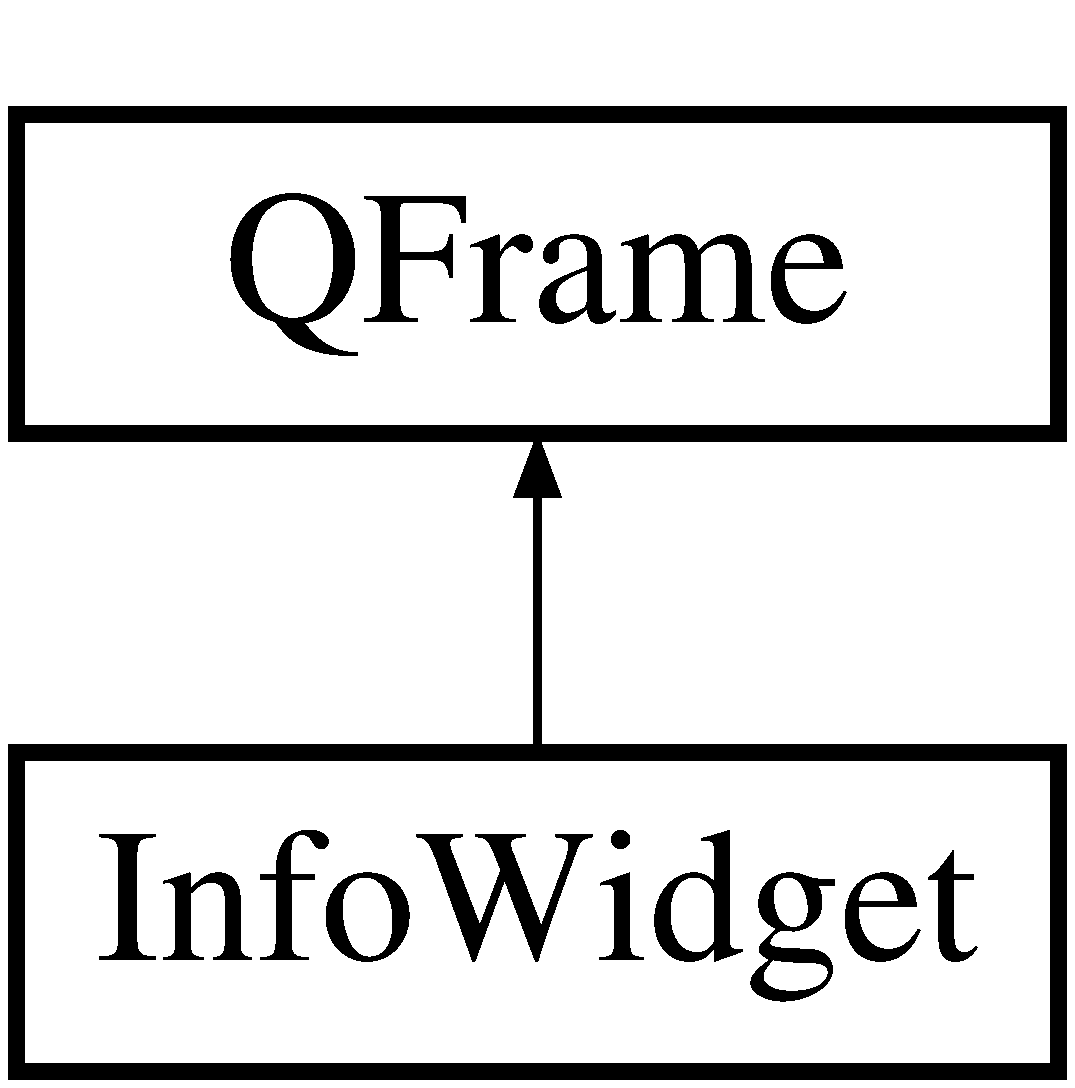
\includegraphics[height=2.000000cm]{classInfoWidget}
\end{center}
\end{figure}
\subsubsection*{Public Member Functions}
\begin{DoxyCompactItemize}
\item 
\mbox{\hyperlink{classInfoWidget_a19f07d861d22be4881361a5a32e86451}{Info\+Widget}} (Q\+Widget $\ast$parent=0)
\item 
\mbox{\hyperlink{classInfoWidget_aefa39a20c91f6dbc8cbc0b6d9bf7623e}{$\sim$\+Info\+Widget}} ()
\item 
void \mbox{\hyperlink{classInfoWidget_a36d29faf6a45282ca2b46ca53de0be19}{set\+Register\+Pointer}} (\mbox{\hyperlink{classRegister}{Register}} $\ast$reg\+Ptr)
\item 
void \mbox{\hyperlink{classInfoWidget_a8a4f1e9fea6f1a9794dffbb264fa7455}{set\+Printed}} (int val)
\item 
void \mbox{\hyperlink{classInfoWidget_a550b6f54475eb5adfba33b4b5f69c6bb}{set\+Total}} (int val)
\item 
void \mbox{\hyperlink{classInfoWidget_a3ff137f58223343fa7ae5b09218a0185}{set\+Icon\+Folder}} (Q\+String path)
\item 
void \mbox{\hyperlink{classInfoWidget_a78af7f055dbb07026ecf1c820b0381bb}{set\+Indicator\+State}} (u\+\_\+int16\+\_\+t state)
\item 
void \mbox{\hyperlink{classInfoWidget_ab17f6cd1820b6946d72c6a42ea3f914b}{set\+Error\+Text}} (\mbox{\hyperlink{classMachineSettings_a87879e13793dbc7c10d4fa18e1236751}{Machine\+Settings\+::\+Machine\+Parameters}} machine\+Parameters, \mbox{\hyperlink{settings_8h_a017dd44e68049ffdd31500a8cd01ba68}{uint16\+\_\+t}} val)
\item 
void \mbox{\hyperlink{classInfoWidget_a1131ca67076ad6951cd2636a7e4e1c7e}{set\+Text}} (Q\+String text)
\end{DoxyCompactItemize}
\subsubsection*{Protected Member Functions}
\begin{DoxyCompactItemize}
\item 
void \mbox{\hyperlink{classInfoWidget_ab9215d8a0db2c91c669dba5e67e27f54}{change\+Event}} (Q\+Event $\ast$event)
\end{DoxyCompactItemize}
\subsubsection*{Private Attributes}
\begin{DoxyCompactItemize}
\item 
Ui\+::\+Info\+Widget $\ast$ \mbox{\hyperlink{classInfoWidget_aac7bf6194c8940ae8bfe6c58ac8a0a43}{ui}}
\item 
Q\+Image \mbox{\hyperlink{classInfoWidget_a0d4c516216ba3df3003c72eec8bf929b}{image\+Home}}
\item 
Q\+Image \mbox{\hyperlink{classInfoWidget_acc842dfe6d29575f2ddbd89cb48f3853}{image\+Lock}}
\item 
Q\+Image \mbox{\hyperlink{classInfoWidget_aff1ea16a7e3fffe12b6bf53ab8ab2df6}{image\+Up}}
\item 
Q\+Image \mbox{\hyperlink{classInfoWidget_a8958069e6c72dde19d74070b0b565d4c}{image\+Arrows}}
\item 
Q\+Image \mbox{\hyperlink{classInfoWidget_a6ca240f5f640fd0ea85e47e9e5d75803}{image\+Emerg}}
\item 
Q\+Image \mbox{\hyperlink{classInfoWidget_abaf1390d58dee5c66125dc58e2aee303}{image\+Warning}}
\item 
Q\+Image \mbox{\hyperlink{classInfoWidget_a0e0b5db9d429867826f370f2a24144da}{image\+Stop\+Hand}}
\item 
Q\+String \mbox{\hyperlink{classInfoWidget_ae0bf133d0a2f93b0536a47fcdad1fbe7}{path\+Icon}}
\item 
Q\+Time \mbox{\hyperlink{classInfoWidget_a2caf54e74e7a24fc5c51ba9c233bce2a}{last\+Time}}
\item 
Q\+Graphics\+Opacity\+Effect $\ast$ \mbox{\hyperlink{classInfoWidget_a08d17f18fb1e38dcf3fe8d8c4974dd22}{effect}} \mbox{[}7\mbox{]}
\item 
\mbox{\hyperlink{classRegister}{Register}} $\ast$ \mbox{\hyperlink{classInfoWidget_a410514814006364f1abb4ce70e15ea90}{local\+Registers}}
\item 
Q\+Settings $\ast$ \mbox{\hyperlink{classInfoWidget_a823b30e65e7e903ad07ae4decc13330d}{err\+Masages}}
\end{DoxyCompactItemize}


\subsubsection{Constructor \& Destructor Documentation}
\mbox{\Hypertarget{classInfoWidget_a19f07d861d22be4881361a5a32e86451}\label{classInfoWidget_a19f07d861d22be4881361a5a32e86451}} 
\index{Info\+Widget@{Info\+Widget}!Info\+Widget@{Info\+Widget}}
\index{Info\+Widget@{Info\+Widget}!Info\+Widget@{Info\+Widget}}
{\footnotesize\ttfamily Info\+Widget\+::\texorpdfstring{Info\+Widget}{InfoWidget} (\begin{DoxyParamCaption}\item[{Q\+Widget $\ast$}]{parent = {\ttfamily 0} }\end{DoxyParamCaption}){\ttfamily [explicit]}} - standard class constructor. Function initialize Q\+Images and load pictures into them, create Q\+Graphics\+Opacity\+Effects and set it to appropriate images, load error messages file to Q\+Settings class object. 

\mbox{\Hypertarget{classInfoWidget_aefa39a20c91f6dbc8cbc0b6d9bf7623e}\label{classInfoWidget_aefa39a20c91f6dbc8cbc0b6d9bf7623e}} 
\index{Info\+Widget@{Info\+Widget}!````~Info\+Widget@{$\sim$\+Info\+Widget}}
\index{````~Info\+Widget@{$\sim$\+Info\+Widget}!Info\+Widget@{Info\+Widget}}
{\footnotesize\ttfamily Info\+Widget\+::\texorpdfstring{$\sim$\+Info\+Widget}{~InfoWidget} (\begin{DoxyParamCaption}{ }\end{DoxyParamCaption})} - standard class destructor.



\subsubsection{Member Function Documentation}
\mbox{\Hypertarget{classInfoWidget_ab9215d8a0db2c91c669dba5e67e27f54}\label{classInfoWidget_ab9215d8a0db2c91c669dba5e67e27f54}} 
\index{Info\+Widget@{Info\+Widget}!change\+Event@{change\+Event}}
\index{change\+Event@{change\+Event}!Info\+Widget@{Info\+Widget}}
{\footnotesize\ttfamily void Info\+Widget\+::\texorpdfstring{change\+Event}{changeEvent} (\begin{DoxyParamCaption}\item[{Q\+Event $\ast$}]{event }\end{DoxyParamCaption}){\ttfamily [protected]}} - reimplementation of default event for QWidget to enable user interface translation. Function called automatically.

\mbox{\Hypertarget{classInfoWidget_ab17f6cd1820b6946d72c6a42ea3f914b}\label{classInfoWidget_ab17f6cd1820b6946d72c6a42ea3f914b}} 
\index{Info\+Widget@{Info\+Widget}!set\+Error\+Text@{set\+Error\+Text}}
\index{set\+Error\+Text@{set\+Error\+Text}!Info\+Widget@{Info\+Widget}}
{\footnotesize\ttfamily void Info\+Widget\+::\texorpdfstring{set\+Error\+Text}{setErrorText} (\begin{DoxyParamCaption}\item[{\mbox{\hyperlink{classMachineSettings_a87879e13793dbc7c10d4fa18e1236751}{Machine\+Settings\+::\+Machine\+Parameters}}}]{machine\+Parameters,  }\item[{\mbox{\hyperlink{settings_8h_a017dd44e68049ffdd31500a8cd01ba68}{uint16\+\_\+t}}}]{val }\end{DoxyParamCaption})} - function to display error message at \textit{labelInfo}. Parameter \textit{machine\+Parameters} used to select text from \hyperlink{classInfoWidget_a823b30e65e7e903ad07ae4decc13330d}{err\+Masages} object. Parameter \textit{val} is unused. Error code, device and other info takes from \hyperlink{classInfoWidget_a410514814006364f1abb4ce70e15ea90}{local\+Registers} :: \hyperlink{classRegister_a109eaf7556eeb67fb1266f2c4be4477ea9bc9f7f42bfc308c9d4d852c34f88266}{master\+Reg\+\_\+\+D\+E\+V\+E\+RR}, \hyperlink{classRegister_a109eaf7556eeb67fb1266f2c4be4477ea8fe2c7e24469c241f73e0e8c4479df5f}{master\+Reg\+\_\+\+E\+RR}, \hyperlink{classRegister_a109eaf7556eeb67fb1266f2c4be4477ea24c2d649cc95e68e1469708ca96ba048}{master\+Reg\+\_\+\+E\+R\+R\+O\+R\+\_\+\+M\+E\+S\+S\+A\+GE} data at function invoke.

\mbox{\Hypertarget{classInfoWidget_a3ff137f58223343fa7ae5b09218a0185}\label{classInfoWidget_a3ff137f58223343fa7ae5b09218a0185}} 
\index{Info\+Widget@{Info\+Widget}!set\+Icon\+Folder@{set\+Icon\+Folder}}
\index{set\+Icon\+Folder@{set\+Icon\+Folder}!Info\+Widget@{Info\+Widget}}
{\footnotesize\ttfamily void Info\+Widget\+::\texorpdfstring{set\+Icon\+Folder}{setIconFolder} (\begin{DoxyParamCaption}\item[{Q\+String}]{path }\end{DoxyParamCaption})} - function to change folder with icons which used on view and update icons. Icon path written to \hyperlink{classInfoWidget_ae0bf133d0a2f93b0536a47fcdad1fbe7}{path\+Icon} variable.

\mbox{\Hypertarget{classInfoWidget_a78af7f055dbb07026ecf1c820b0381bb}\label{classInfoWidget_a78af7f055dbb07026ecf1c820b0381bb}} 
\index{Info\+Widget@{Info\+Widget}!set\+Indicator\+State@{set\+Indicator\+State}}
\index{set\+Indicator\+State@{set\+Indicator\+State}!Info\+Widget@{Info\+Widget}}
{\footnotesize\ttfamily void Info\+Widget\+::\texorpdfstring{set\+Indicator\+State}{setIndicatorState} (\begin{DoxyParamCaption}\item[{u\+\_\+int16\+\_\+t}]{state }\end{DoxyParamCaption})} - function to set state of indicators on widget. State describe which indicators will be visible or hidden. State sets by master board of machine, when \hyperlink{structRegister_1_1MasterReg___1_1reg}{Register\+::\+Master\+Reg\+\_\+\+::reg} field \hyperlink{structRegister_1_1MasterReg___1_1reg_aa5111a7f8eddbd8f8d6c92e23f326946}{master\+Reg\+\_\+\+E\+KR} updates its value.

\mbox{\Hypertarget{classInfoWidget_a8a4f1e9fea6f1a9794dffbb264fa7455}\label{classInfoWidget_a8a4f1e9fea6f1a9794dffbb264fa7455}} 
\index{Info\+Widget@{Info\+Widget}!set\+Printed@{set\+Printed}}
\index{set\+Printed@{set\+Printed}!Info\+Widget@{Info\+Widget}}
{\footnotesize\ttfamily void Info\+Widget\+::\texorpdfstring{set\+Printed()}{setPrinted()} (\begin{DoxyParamCaption}\item[{int}]{val }\end{DoxyParamCaption})} - function to update values on \textit{label\+Printed} and on \textit{label\+DZH}. Value \textit{label\+DZH} updates automatically by time delay calculation between invokes of function.

\mbox{\Hypertarget{classInfoWidget_a36d29faf6a45282ca2b46ca53de0be19}\label{classInfoWidget_a36d29faf6a45282ca2b46ca53de0be19}} 
\index{Info\+Widget@{Info\+Widget}!set\+Register\+Pointer@{set\+Register\+Pointer}}
\index{set\+Register\+Pointer@{set\+Register\+Pointer}!Info\+Widget@{Info\+Widget}}
{\footnotesize\ttfamily void Info\+Widget\+::\texorpdfstring{set\+Register\+Pointer}{setRegisterPointer} (\begin{DoxyParamCaption}\item[{\mbox{\hyperlink{classRegister}{Register}} $\ast$}]{reg\+Ptr }\end{DoxyParamCaption})}  - function to set pointer to \hyperlink{classRegister}{Register} class object. In a whole program used only one sample of class and pointer (\hyperlink{classMainWindow_aead190b1b4ca3ce95076274ab2ae6f84}{registers}) set from parent object. 

\mbox{\Hypertarget{classInfoWidget_a1131ca67076ad6951cd2636a7e4e1c7e}\label{classInfoWidget_a1131ca67076ad6951cd2636a7e4e1c7e}} 
\index{Info\+Widget@{Info\+Widget}!set\+Text@{set\+Text}}
\index{set\+Text@{set\+Text}!Info\+Widget@{Info\+Widget}}
{\footnotesize\ttfamily void Info\+Widget\+::\texorpdfstring{set\+Text}{setText} (\begin{DoxyParamCaption}\item[{Q\+String}]{text }\end{DoxyParamCaption})} - function to set custom text on \textit{label\+Info}.

\mbox{\Hypertarget{classInfoWidget_a550b6f54475eb5adfba33b4b5f69c6bb}\label{classInfoWidget_a550b6f54475eb5adfba33b4b5f69c6bb}} 
\index{Info\+Widget@{Info\+Widget}!set\+Total@{set\+Total}}
\index{set\+Total@{set\+Total}!Info\+Widget@{Info\+Widget}}
{\footnotesize\ttfamily void Info\+Widget\+::\texorpdfstring{set\+Total}{setTotal} (\begin{DoxyParamCaption}\item[{int}]{val }\end{DoxyParamCaption})}  - function to update values on \textit{label\+Total}.

\subsubsection{Member Data Documentation}
\mbox{\Hypertarget{classInfoWidget_a08d17f18fb1e38dcf3fe8d8c4974dd22}\label{classInfoWidget_a08d17f18fb1e38dcf3fe8d8c4974dd22}} 
\index{Info\+Widget@{Info\+Widget}!effect@{effect}}
\index{effect@{effect}!Info\+Widget@{Info\+Widget}}
{\footnotesize\ttfamily Q\+Graphics\+Opacity\+Effect$\ast$ Info\+Widget\+::\texorpdfstring{effect}{effect}\mbox{[}7\mbox{]}{\ttfamily [private]}}

\mbox{\Hypertarget{classInfoWidget_a823b30e65e7e903ad07ae4decc13330d}\label{classInfoWidget_a823b30e65e7e903ad07ae4decc13330d}} 
\index{Info\+Widget@{Info\+Widget}!err\+Masages@{err\+Masages}}
\index{err\+Masages@{err\+Masages}!Info\+Widget@{Info\+Widget}}
{\footnotesize\ttfamily Q\+Settings$\ast$ Info\+Widget\+::\texorpdfstring{err\+Masages}{errMasages}{\ttfamily [private]}}

\mbox{\Hypertarget{classInfoWidget_a8958069e6c72dde19d74070b0b565d4c}\label{classInfoWidget_a8958069e6c72dde19d74070b0b565d4c}} 
\index{Info\+Widget@{Info\+Widget}!image\+Arrows@{image\+Arrows}}
\index{image\+Arrows@{image\+Arrows}!Info\+Widget@{Info\+Widget}}
{\footnotesize\ttfamily Q\+Image Info\+Widget\+::\texorpdfstring{image\+Arrows}{imageArrows}{\ttfamily [private]}}

\mbox{\Hypertarget{classInfoWidget_a6ca240f5f640fd0ea85e47e9e5d75803}\label{classInfoWidget_a6ca240f5f640fd0ea85e47e9e5d75803}} 
\index{Info\+Widget@{Info\+Widget}!image\+Emerg@{image\+Emerg}}
\index{image\+Emerg@{image\+Emerg}!Info\+Widget@{Info\+Widget}}
{\footnotesize\ttfamily Q\+Image Info\+Widget\+::\texorpdfstring{image\+Emerg}{imageEmerg}{\ttfamily [private]}}

\mbox{\Hypertarget{classInfoWidget_a0d4c516216ba3df3003c72eec8bf929b}\label{classInfoWidget_a0d4c516216ba3df3003c72eec8bf929b}} 
\index{Info\+Widget@{Info\+Widget}!image\+Home@{image\+Home}}
\index{image\+Home@{image\+Home}!Info\+Widget@{Info\+Widget}}
{\footnotesize\ttfamily Q\+Image Info\+Widget\+::\texorpdfstring{image\+Home}{imageHome}{\ttfamily [private]}}

\mbox{\Hypertarget{classInfoWidget_acc842dfe6d29575f2ddbd89cb48f3853}\label{classInfoWidget_acc842dfe6d29575f2ddbd89cb48f3853}} 
\index{Info\+Widget@{Info\+Widget}!image\+Lock@{image\+Lock}}
\index{image\+Lock@{image\+Lock}!Info\+Widget@{Info\+Widget}}
{\footnotesize\ttfamily Q\+Image Info\+Widget\+::\texorpdfstring{image\+Lock}{imageLock}{\ttfamily [private]}}

\mbox{\Hypertarget{classInfoWidget_a0e0b5db9d429867826f370f2a24144da}\label{classInfoWidget_a0e0b5db9d429867826f370f2a24144da}} 
\index{Info\+Widget@{Info\+Widget}!image\+Stop\+Hand@{image\+Stop\+Hand}}
\index{image\+Stop\+Hand@{image\+Stop\+Hand}!Info\+Widget@{Info\+Widget}}
{\footnotesize\ttfamily Q\+Image Info\+Widget\+::\texorpdfstring{image\+Stop\+Hand}{imageStopHand}{\ttfamily [private]}}

\mbox{\Hypertarget{classInfoWidget_aff1ea16a7e3fffe12b6bf53ab8ab2df6}\label{classInfoWidget_aff1ea16a7e3fffe12b6bf53ab8ab2df6}} 
\index{Info\+Widget@{Info\+Widget}!image\+Up@{image\+Up}}
\index{image\+Up@{image\+Up}!Info\+Widget@{Info\+Widget}}
{\footnotesize\ttfamily Q\+Image Info\+Widget\+::\texorpdfstring{image\+Up}{imageUp}{\ttfamily [private]}}

\mbox{\Hypertarget{classInfoWidget_abaf1390d58dee5c66125dc58e2aee303}\label{classInfoWidget_abaf1390d58dee5c66125dc58e2aee303}} 
\index{Info\+Widget@{Info\+Widget}!image\+Warning@{image\+Warning}}
\index{image\+Warning@{image\+Warning}!Info\+Widget@{Info\+Widget}}
{\footnotesize\ttfamily Q\+Image Info\+Widget\+::\texorpdfstring{image\+Warning}{imageWarning}{\ttfamily [private]}}

\mbox{\Hypertarget{classInfoWidget_a2caf54e74e7a24fc5c51ba9c233bce2a}\label{classInfoWidget_a2caf54e74e7a24fc5c51ba9c233bce2a}} 
\index{Info\+Widget@{Info\+Widget}!last\+Time@{last\+Time}}
\index{last\+Time@{last\+Time}!Info\+Widget@{Info\+Widget}}
{\footnotesize\ttfamily Q\+Time Info\+Widget\+::\texorpdfstring{last\+Time}{lastTime}{\ttfamily [private]}}

\mbox{\Hypertarget{classInfoWidget_a410514814006364f1abb4ce70e15ea90}\label{classInfoWidget_a410514814006364f1abb4ce70e15ea90}} 
\index{Info\+Widget@{Info\+Widget}!local\+Registers@{local\+Registers}}
\index{local\+Registers@{local\+Registers}!Info\+Widget@{Info\+Widget}}
{\footnotesize\ttfamily \mbox{\hyperlink{classRegister}{Register}}$\ast$ Info\+Widget\+::\texorpdfstring{local\+Registers}{localRegisters}{\ttfamily [private]}}

\mbox{\Hypertarget{classInfoWidget_ae0bf133d0a2f93b0536a47fcdad1fbe7}\label{classInfoWidget_ae0bf133d0a2f93b0536a47fcdad1fbe7}} 
\index{Info\+Widget@{Info\+Widget}!path\+Icon@{path\+Icon}}
\index{path\+Icon@{path\+Icon}!Info\+Widget@{Info\+Widget}}
{\footnotesize\ttfamily Q\+String Info\+Widget\+::\texorpdfstring{path\+Icon}{pathIcon}{\ttfamily [private]}}


The documentation for this class was generated from the following files\+:\begin{DoxyCompactItemize}
\item 
\mbox{\hyperlink{infowidget_8h}{infowidget.\+h}}\item 
\mbox{\hyperlink{infowidget_8cpp}{infowidget.\+cpp}}\end{DoxyCompactItemize}
\newpage
\hypertarget{classKeyboardButton}{}\subsection{Keyboard\+Button Class Reference}
\label{classKeyboardButton}\index{Keyboard\+Button@{Keyboard\+Button}}
Reimplementation of class of QPushButton. Added \hyperlink{classKeyboardButton_a8979a4765bd83241a9a253211ec03774}{character} variable and signal \hyperlink{classKeyboardButton_a6c6694c8330565de78f47f3c5fe11d06}{clicked}(...)

{\ttfamily \#include $<$keyboarddialog.\+h$>$}

Inheritance diagram for Keyboard\+Button\+:\begin{figure}[H]
\begin{center}
\leavevmode
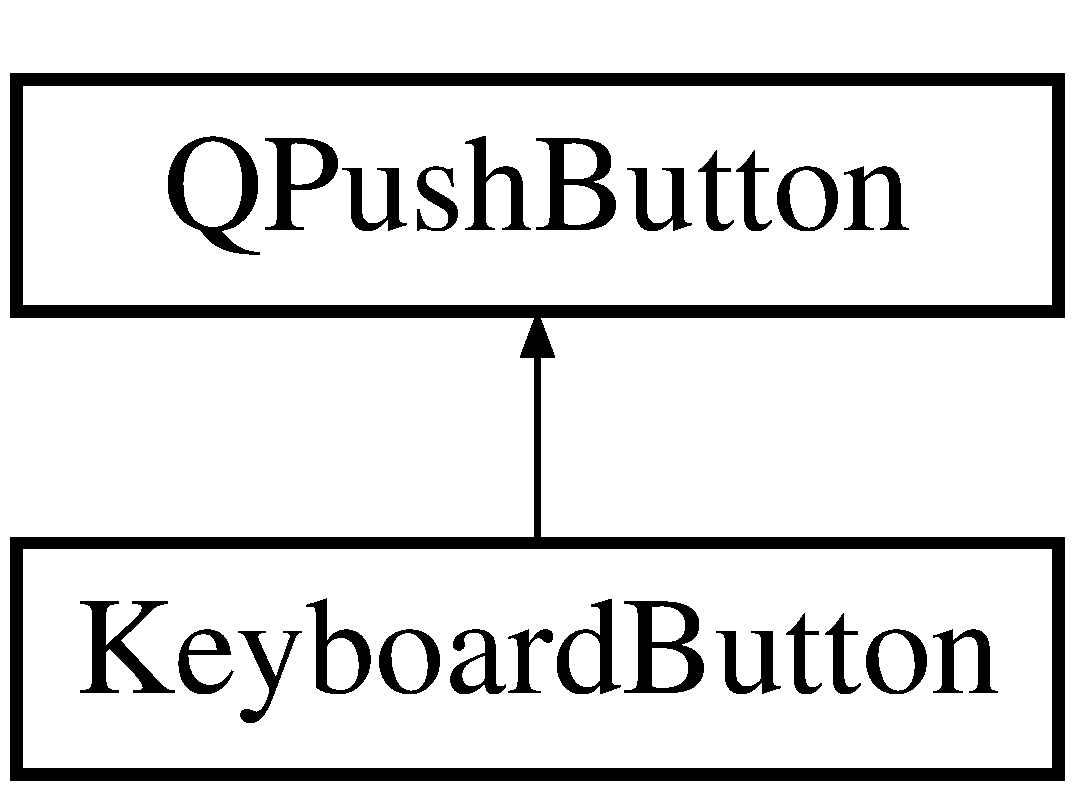
\includegraphics[height=2.000000cm]{classKeyboardButton}
\end{center}
\end{figure}
\subsubsection*{Signals}
\begin{DoxyCompactItemize}
\item 
void \mbox{\hyperlink{classKeyboardButton_a6c6694c8330565de78f47f3c5fe11d06}{clicked}} (Q\+String \mbox{\hyperlink{classKeyboardButton_a8979a4765bd83241a9a253211ec03774}{character}})
\end{DoxyCompactItemize}
\subsubsection*{Public Member Functions}
\begin{DoxyCompactItemize}
\item 
\mbox{\hyperlink{classKeyboardButton_ac2eac39f778e78dad45bac730e6a30bd}{Keyboard\+Button}} (Q\+String \mbox{\hyperlink{classKeyboardButton_a8979a4765bd83241a9a253211ec03774}{character}})
\item 
Q\+String \mbox{\hyperlink{classKeyboardButton_a44c7448a3bae4dbc1a3f4f7ecbaeafbd}{get\+Character}} ()
\item 
void \mbox{\hyperlink{classKeyboardButton_aca3123dc3392dc90f631bf8004a71061}{set\+Character}} (Q\+String str)
\end{DoxyCompactItemize}
\subsubsection*{Private Slots}
\begin{DoxyCompactItemize}
\item 
void \mbox{\hyperlink{classKeyboardButton_a518fc800cf7acf3b2a9614c7bfe74f93}{this\+Clicked}} ()
\end{DoxyCompactItemize}
\subsubsection*{Private Attributes}
\begin{DoxyCompactItemize}
\item 
Q\+String \mbox{\hyperlink{classKeyboardButton_a8979a4765bd83241a9a253211ec03774}{character}}
\end{DoxyCompactItemize}


\subsubsection{Constructor \& Destructor Documentation}
\mbox{\Hypertarget{classKeyboardButton_ac2eac39f778e78dad45bac730e6a30bd}\label{classKeyboardButton_ac2eac39f778e78dad45bac730e6a30bd}} 
\index{Keyboard\+Button@{Keyboard\+Button}!Keyboard\+Button@{Keyboard\+Button}}
\index{Keyboard\+Button@{Keyboard\+Button}!Keyboard\+Button@{Keyboard\+Button}}
{\footnotesize\ttfamily Keyboard\+Button\+::\texorpdfstring{Keyboard\+Button}{KeyboardButton} (\begin{DoxyParamCaption}\item[{Q\+String}]{character }\end{DoxyParamCaption})} - constructor of class with \hyperlink{classKeyboardButton_a8979a4765bd83241a9a253211ec03774}{character} variable initialization. Value of parameter sets like a text on button.

\subsubsection{Member Function Documentation}
\mbox{\Hypertarget{classKeyboardButton_a6c6694c8330565de78f47f3c5fe11d06}\label{classKeyboardButton_a6c6694c8330565de78f47f3c5fe11d06}} 
\index{Keyboard\+Button@{Keyboard\+Button}!clicked@{clicked}}
\index{clicked@{clicked}!Keyboard\+Button@{Keyboard\+Button}}
{\footnotesize\ttfamily void Keyboard\+Button\+::\texorpdfstring{clicked}{clicked} (\begin{DoxyParamCaption}\item[{Q\+String}]{character }\end{DoxyParamCaption}){\ttfamily [signal]}} - signal which emit when button is clicked by \hyperlink{classKeyboardButton_a518fc800cf7acf3b2a9614c7bfe74f93}{this\+Clicked}(..) function.

\mbox{\Hypertarget{classKeyboardButton_a44c7448a3bae4dbc1a3f4f7ecbaeafbd}\label{classKeyboardButton_a44c7448a3bae4dbc1a3f4f7ecbaeafbd}} 
\index{Keyboard\+Button@{Keyboard\+Button}!get\+Character@{get\+Character}}
\index{get\+Character@{get\+Character}!Keyboard\+Button@{Keyboard\+Button}}
{\footnotesize\ttfamily Q\+String Keyboard\+Button\+::\texorpdfstring{get\+Character}{getCharacter} (\begin{DoxyParamCaption}{ }\end{DoxyParamCaption})} - function to get \hyperlink{classKeyboardButton_a8979a4765bd83241a9a253211ec03774}{character} variable.

\mbox{\Hypertarget{classKeyboardButton_aca3123dc3392dc90f631bf8004a71061}\label{classKeyboardButton_aca3123dc3392dc90f631bf8004a71061}} 
\index{Keyboard\+Button@{Keyboard\+Button}!set\+Character@{set\+Character}}
\index{set\+Character@{set\+Character}!Keyboard\+Button@{Keyboard\+Button}}
{\footnotesize\ttfamily void Keyboard\+Button\+::\texorpdfstring{set\+Character}{setCharacter} (\begin{DoxyParamCaption}\item[{Q\+String}]{str }\end{DoxyParamCaption})} - function to set \hyperlink{classKeyboardButton_a8979a4765bd83241a9a253211ec03774}{character} variable.

\mbox{\Hypertarget{classKeyboardButton_a518fc800cf7acf3b2a9614c7bfe74f93}\label{classKeyboardButton_a518fc800cf7acf3b2a9614c7bfe74f93}} 
\index{Keyboard\+Button@{Keyboard\+Button}!this\+Clicked@{this\+Clicked}}
\index{this\+Clicked@{this\+Clicked}!Keyboard\+Button@{Keyboard\+Button}}
{\footnotesize\ttfamily void Keyboard\+Button\+::\texorpdfstring{this\+Clicked}{thisClicked} (\begin{DoxyParamCaption}{ }\end{DoxyParamCaption}){\ttfamily [inline]}, {\ttfamily [private]}, {\ttfamily [slot]}} - function which called by standard \textit{Q\+Push\+Button::clicked()} signal and emit \hyperlink{classKeyboardButton_a6c6694c8330565de78f47f3c5fe11d06}{clicked}(...) signal.



\subsubsection{Member Data Documentation}
\mbox{\Hypertarget{classKeyboardButton_a8979a4765bd83241a9a253211ec03774}\label{classKeyboardButton_a8979a4765bd83241a9a253211ec03774}} 
\index{Keyboard\+Button@{Keyboard\+Button}!character@{character}}
\index{character@{character}!Keyboard\+Button@{Keyboard\+Button}}
{\footnotesize\ttfamily Q\+String Keyboard\+Button\+::\texorpdfstring{character}{character}{\ttfamily [private]}}



The documentation for this class was generated from the following files\+:\begin{DoxyCompactItemize}
\item 
\mbox{\hyperlink{keyboarddialog_8h}{keyboarddialog.\+h}}\item 
\mbox{\hyperlink{keyboarddialog_8cpp}{keyboarddialog.\+cpp}}\end{DoxyCompactItemize}
\newpage
\hypertarget{classKeyboardDialog}{}\subsection{Keyboard\+Dialog Class Reference}
\label{classKeyboardDialog}\index{Keyboard\+Dialog@{Keyboard\+Dialog}}


{\ttfamily \#include $<$keyboarddialog.\+h$>$}

Inheritance diagram for Keyboard\+Dialog\+:\begin{figure}[H]
\begin{center}
\leavevmode
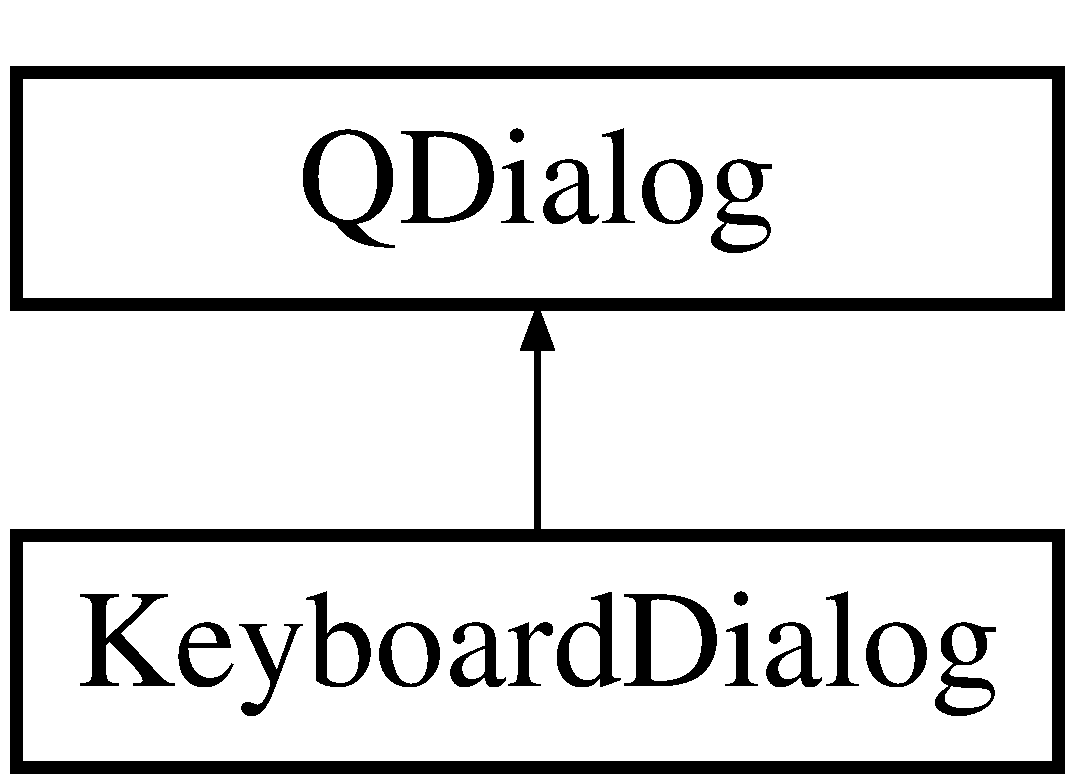
\includegraphics[height=2.000000cm]{classKeyboardDialog}
\end{center}
\end{figure}
\subsubsection*{Public Types}
\begin{DoxyCompactItemize}
\item 
enum \mbox{\hyperlink{classKeyboardDialog_a7151e64aa0ea07c96bcb582722f39b70}{Keyboard\+Position\+\_\+}} \{ \mbox{\hyperlink{classKeyboardDialog_a7151e64aa0ea07c96bcb582722f39b70a39f2161b184336fbdea336949a1c432b}{Bottom}}, 
\mbox{\hyperlink{classKeyboardDialog_a7151e64aa0ea07c96bcb582722f39b70ae3f3821683c5ddc59b87508d3f67d6eb}{Custom}}
 \}
\item 
typedef enum \mbox{\hyperlink{classKeyboardDialog_a7151e64aa0ea07c96bcb582722f39b70}{Keyboard\+Dialog\+::\+Keyboard\+Position\+\_\+}} \mbox{\hyperlink{classKeyboardDialog_a15d9e75dad34470ec9872ca45b63e510}{Keyboard\+Position}}
\end{DoxyCompactItemize}
\subsubsection*{Signals}
\begin{DoxyCompactItemize}
\item 
void \mbox{\hyperlink{classKeyboardDialog_a60a486df4f0be9c78a1ac6615aea3d9e}{key\+Clicked}} ()
\end{DoxyCompactItemize}
\subsubsection*{Public Member Functions}
\begin{DoxyCompactItemize}
\item 
\mbox{\hyperlink{classKeyboardDialog_afb05238e8046e60d2c25e022c810f665}{Keyboard\+Dialog}} (Q\+Widget $\ast$parent=0, Q\+String window\+Title=\char`\"{}Keyboard\char`\"{})
\item 
\mbox{\hyperlink{classKeyboardDialog_aa430c1c9aaa94d79e8d83aec7753c21a}{$\sim$\+Keyboard\+Dialog}} ()
\item 
void \mbox{\hyperlink{classKeyboardDialog_a7a276672e902fa810e3c06047992fd69}{buttons\+To\+Upper}} ()
\item 
void \mbox{\hyperlink{classKeyboardDialog_af8f1934505c0f78ad6b2a1e6aeb4cb2e}{buttons\+To\+Lower}} ()
\end{DoxyCompactItemize}
\subsubsection*{Static Public Member Functions}
\begin{DoxyCompactItemize}
\item 
static Q\+String \mbox{\hyperlink{classKeyboardDialog_ab76b5389fc4f4628b2fa6897da0efa28}{get\+Text}} (Q\+Widget $\ast$parent=0, Q\+String window\+Title=\char`\"{}Keyboard\char`\"{}, Keyboard\+Position position=\mbox{\hyperlink{classKeyboardDialog_a7151e64aa0ea07c96bcb582722f39b70ae3f3821683c5ddc59b87508d3f67d6eb}{Custom}})
\end{DoxyCompactItemize}
\subsubsection*{Protected Member Functions}
\begin{DoxyCompactItemize}
\item 
void \mbox{\hyperlink{classKeyboardDialog_a0c118ece8b936e3393bb3124415dde6b}{change\+Event}} (Q\+Event $\ast$event)
\end{DoxyCompactItemize}
\subsubsection*{Private Slots}
\begin{DoxyCompactItemize}
\item 
void \mbox{\hyperlink{classKeyboardDialog_ae6dc8c69ff16942b5185fa97423b9cc0}{append\+To\+Line\+Edit}} (Q\+String str)
\item 
void \mbox{\hyperlink{classKeyboardDialog_a471f014a3c1a8ba612fce0ef2bc135a4}{backspace}} ()
\item 
void \mbox{\hyperlink{classKeyboardDialog_ab5b4e6cdc245ddd1709a9bff9767c1c7}{submit\+Text}} ()
\item 
void \mbox{\hyperlink{classKeyboardDialog_a991a2385014b01ad257f07092cf98b11}{shift}} ()
\item 
void \mbox{\hyperlink{classKeyboardDialog_a666a29c8db901ad52b14c5b40e333608}{deshift}} ()
\item 
void \mbox{\hyperlink{classKeyboardDialog_a0baaa948c0434c2f1fe6056319fcc4e2}{caps\+Lock}} ()
\item 
void \mbox{\hyperlink{classKeyboardDialog_ab13992b7c1c3025bb96826d4da17b931}{some\+Key\+Clicked}} ()
\item 
void \mbox{\hyperlink{classKeyboardDialog_add2f730a4a7439b88b98140fbc7d09f9}{dash\+Underscore\+Switch}} (bool shifted=false)
\end{DoxyCompactItemize}
\subsubsection*{Private Attributes}
\begin{DoxyCompactItemize}
\item 
Q\+String\+List \mbox{\hyperlink{classKeyboardDialog_a6a084cc6108c5fc50c05f567d241af8b}{characters}}
\item 
Ui\+::\+Keyboard\+Dialog $\ast$ \mbox{\hyperlink{classKeyboardDialog_a6264cc8da370d38ab8a4b7a8a6539b0f}{ui}}
\item 
Q\+List$<$ \mbox{\hyperlink{classKeyboardButton}{Keyboard\+Button}} $\ast$ $>$ \mbox{\hyperlink{classKeyboardDialog_a334172863bd0cdc1fd2792b935c3dc3e}{buttons}}
\item 
\mbox{\hyperlink{classKeyboardButton}{Keyboard\+Button}} $\ast$ \mbox{\hyperlink{classKeyboardDialog_a9cbeeb36e8ca22c07310316f67a95832}{dash\+Underscore\+Button}}
\item 
Q\+String \mbox{\hyperlink{classKeyboardDialog_a840896bed408c1e8cdb44e27dee9d195}{text}}
\item 
bool \mbox{\hyperlink{classKeyboardDialog_ac42a101f1ede0b3565cbc7d87bff20b4}{caps\+Lock\+Flag}}
\item 
bool \mbox{\hyperlink{classKeyboardDialog_aad63f68247d9c00db715a2afb1bf9bc3}{shift\+Flag}}
\end{DoxyCompactItemize}


\subsubsection{Member Typedef Documentation}
\mbox{\Hypertarget{classKeyboardDialog_a15d9e75dad34470ec9872ca45b63e510}\label{classKeyboardDialog_a15d9e75dad34470ec9872ca45b63e510}} 
\index{Keyboard\+Dialog@{Keyboard\+Dialog}!Keyboard\+Position@{Keyboard\+Position}}
\index{Keyboard\+Position@{Keyboard\+Position}!Keyboard\+Dialog@{Keyboard\+Dialog}}
{\footnotesize\ttfamily typedef enum \mbox{\hyperlink{classKeyboardDialog_a7151e64aa0ea07c96bcb582722f39b70}{Keyboard\+Dialog\+::\+Keyboard\+Position\+\_\+}} \mbox{\hyperlink{classKeyboardDialog_a15d9e75dad34470ec9872ca45b63e510}{Keyboard\+Dialog\+::\texorpdfstring{Keyboard\+Position}{KeyboardPosition}}}}



\subsubsection{Member Enumeration Documentation}
\mbox{\Hypertarget{classKeyboardDialog_a7151e64aa0ea07c96bcb582722f39b70}\label{classKeyboardDialog_a7151e64aa0ea07c96bcb582722f39b70}} 
\index{Keyboard\+Dialog@{Keyboard\+Dialog}!Keyboard\+Position\+\_\+@{Keyboard\+Position\+\_\+}}
\index{Keyboard\+Position\+\_\+@{Keyboard\+Position\+\_\+}!Keyboard\+Dialog@{Keyboard\+Dialog}}
{\footnotesize\ttfamily enum \mbox{\hyperlink{classKeyboardDialog_a7151e64aa0ea07c96bcb582722f39b70}{Keyboard\+Dialog\+::\texorpdfstring{Keyboard\+Position\+\_\+}{KeyboardPosition\_}}}}

\begin{DoxyEnumFields}{Enumerator}
\raisebox{\heightof{T}}[0pt][0pt]{\index{Bottom@{Bottom}!Keyboard\+Dialog@{Keyboard\+Dialog}}\index{Keyboard\+Dialog@{Keyboard\+Dialog}!Bottom@{Bottom}}}\mbox{\Hypertarget{classKeyboardDialog_a7151e64aa0ea07c96bcb582722f39b70a39f2161b184336fbdea336949a1c432b}\label{classKeyboardDialog_a7151e64aa0ea07c96bcb582722f39b70a39f2161b184336fbdea336949a1c432b}} 
Bottom&\\
\hline

\raisebox{\heightof{T}}[0pt][0pt]{\index{Custom@{Custom}!Keyboard\+Dialog@{Keyboard\+Dialog}}\index{Keyboard\+Dialog@{Keyboard\+Dialog}!Custom@{Custom}}}\mbox{\Hypertarget{classKeyboardDialog_a7151e64aa0ea07c96bcb582722f39b70ae3f3821683c5ddc59b87508d3f67d6eb}\label{classKeyboardDialog_a7151e64aa0ea07c96bcb582722f39b70ae3f3821683c5ddc59b87508d3f67d6eb}} 
Custom&\\
\hline

\end{DoxyEnumFields}


\subsubsection{Constructor \& Destructor Documentation}
\mbox{\Hypertarget{classKeyboardDialog_afb05238e8046e60d2c25e022c810f665}\label{classKeyboardDialog_afb05238e8046e60d2c25e022c810f665}} 
\index{Keyboard\+Dialog@{Keyboard\+Dialog}!Keyboard\+Dialog@{Keyboard\+Dialog}}
\index{Keyboard\+Dialog@{Keyboard\+Dialog}!Keyboard\+Dialog@{Keyboard\+Dialog}}
{\footnotesize\ttfamily Keyboard\+Dialog\+::\texorpdfstring{Keyboard\+Dialog}{KeyboardDialog} (\begin{DoxyParamCaption}\item[{Q\+Widget $\ast$}]{parent = {\ttfamily 0},  }\item[{Q\+String}]{window\+Title = {\ttfamily \char`\"{}Keyboard\char`\"{}} }\end{DoxyParamCaption}){\ttfamily [explicit]}} - constructor of class. In function fill \hyperlink{classKeyboardDialog_a6a084cc6108c5fc50c05f567d241af8b}{characters} and \hyperlink{classKeyboardDialog_a334172863bd0cdc1fd2792b935c3dc3e}{buttons} lists, create connection for functional buttons, and make layout of that widget on window. Parameter \textit{windowTitle} used to put it on window top panel.

\mbox{\Hypertarget{classKeyboardDialog_aa430c1c9aaa94d79e8d83aec7753c21a}\label{classKeyboardDialog_aa430c1c9aaa94d79e8d83aec7753c21a}} 
\index{Keyboard\+Dialog@{Keyboard\+Dialog}!````~Keyboard\+Dialog@{$\sim$\+Keyboard\+Dialog}}
\index{````~Keyboard\+Dialog@{$\sim$\+Keyboard\+Dialog}!Keyboard\+Dialog@{Keyboard\+Dialog}}
{\footnotesize\ttfamily Keyboard\+Dialog\+::\texorpdfstring{$\sim$\+Keyboard\+Dialog}{~KeyboardDialog} (\begin{DoxyParamCaption}{ }\end{DoxyParamCaption})} - standard Q\+Dialog destructor.



\subsubsection{Member Function Documentation}
\mbox{\Hypertarget{classKeyboardDialog_ae6dc8c69ff16942b5185fa97423b9cc0}\label{classKeyboardDialog_ae6dc8c69ff16942b5185fa97423b9cc0}} 
\index{Keyboard\+Dialog@{Keyboard\+Dialog}!append\+To\+Line\+Edit@{append\+To\+Line\+Edit}}
\index{append\+To\+Line\+Edit@{append\+To\+Line\+Edit}!Keyboard\+Dialog@{Keyboard\+Dialog}}
{\footnotesize\ttfamily void Keyboard\+Dialog\+::\texorpdfstring{append\+To\+Line\+Edit}{appendToLineEdit} (\begin{DoxyParamCaption}\item[{Q\+String}]{str }\end{DoxyParamCaption}){\ttfamily [private]}, {\ttfamily [slot]}} - function which is connected to every object in \hyperlink{classKeyboardDialog_a334172863bd0cdc1fd2792b935c3dc3e}{buttons} list and put appropriate symbol at last position at \textit{line\+Edit}. Symbol contains in parameter \textit{str}.

\mbox{\Hypertarget{classKeyboardDialog_a471f014a3c1a8ba612fce0ef2bc135a4}\label{classKeyboardDialog_a471f014a3c1a8ba612fce0ef2bc135a4}} 
\index{Keyboard\+Dialog@{Keyboard\+Dialog}!backspace@{backspace}}
\index{backspace@{backspace}!Keyboard\+Dialog@{Keyboard\+Dialog}}
{\footnotesize\ttfamily void Keyboard\+Dialog\+::\texorpdfstring{backspace}{backspace} (\begin{DoxyParamCaption}{ }\end{DoxyParamCaption}){\ttfamily [private]}, {\ttfamily [slot]}} - function for removing last symbol at \textit{line\+Edit}. invoked by \textit{pb\+Backspace}.

\mbox{\Hypertarget{classKeyboardDialog_af8f1934505c0f78ad6b2a1e6aeb4cb2e}\label{classKeyboardDialog_af8f1934505c0f78ad6b2a1e6aeb4cb2e}} 
\index{Keyboard\+Dialog@{Keyboard\+Dialog}!buttons\+To\+Lower@{buttons\+To\+Lower}}
\index{buttons\+To\+Lower@{buttons\+To\+Lower}!Keyboard\+Dialog@{Keyboard\+Dialog}}
{\footnotesize\ttfamily void Keyboard\+Dialog\+::\texorpdfstring{buttons\+To\+Lower}{buttonsToLower} (\begin{DoxyParamCaption}{ }\end{DoxyParamCaption})} - function to change text on keyboard and symbol to lower register.

\mbox{\Hypertarget{classKeyboardDialog_a7a276672e902fa810e3c06047992fd69}\label{classKeyboardDialog_a7a276672e902fa810e3c06047992fd69}} 
\index{Keyboard\+Dialog@{Keyboard\+Dialog}!buttons\+To\+Upper@{buttons\+To\+Upper}}
\index{buttons\+To\+Upper@{buttons\+To\+Upper}!Keyboard\+Dialog@{Keyboard\+Dialog}}
{\footnotesize\ttfamily void Keyboard\+Dialog\+::\texorpdfstring{buttons\+To\+Upper}{buttonsToUpper} (\begin{DoxyParamCaption}{ }\end{DoxyParamCaption})} - function to change text on keyboard and symbol to higher register.

\mbox{\Hypertarget{classKeyboardDialog_a0baaa948c0434c2f1fe6056319fcc4e2}\label{classKeyboardDialog_a0baaa948c0434c2f1fe6056319fcc4e2}} 
\index{Keyboard\+Dialog@{Keyboard\+Dialog}!caps\+Lock@{caps\+Lock}}
\index{caps\+Lock@{caps\+Lock}!Keyboard\+Dialog@{Keyboard\+Dialog}}
{\footnotesize\ttfamily void Keyboard\+Dialog\+::\texorpdfstring{caps\+Lock}{capsLock} (\begin{DoxyParamCaption}{ }\end{DoxyParamCaption}){\ttfamily [private]}, {\ttfamily [slot]}} - function to call \hyperlink{classKeyboardDialog_a7a276672e902fa810e3c06047992fd69}{buttons\+To\+Upper}(...) or \hyperlink{classKeyboardDialog_af8f1934505c0f78ad6b2a1e6aeb4cb2e}{buttons\+To\+Lower}(...) function appropriate to state of \hyperlink{classKeyboardDialog_ac42a101f1ede0b3565cbc7d87bff20b4}{caps\+Lock\+Flag} and invert \hyperlink{classKeyboardDialog_ac42a101f1ede0b3565cbc7d87bff20b4}{caps\+Lock\+Flag} value.

\mbox{\Hypertarget{classKeyboardDialog_a0c118ece8b936e3393bb3124415dde6b}\label{classKeyboardDialog_a0c118ece8b936e3393bb3124415dde6b}} 
\index{Keyboard\+Dialog@{Keyboard\+Dialog}!change\+Event@{change\+Event}}
\index{change\+Event@{change\+Event}!Keyboard\+Dialog@{Keyboard\+Dialog}}
{\footnotesize\ttfamily void Keyboard\+Dialog\+::\texorpdfstring{change\+Event}{changeEvent} (\begin{DoxyParamCaption}\item[{Q\+Event $\ast$}]{event }\end{DoxyParamCaption}){\ttfamily [protected]}} - reimplementation of default event for QWidget to enable user interface translation. Function called automatically.

\mbox{\Hypertarget{classKeyboardDialog_add2f730a4a7439b88b98140fbc7d09f9}\label{classKeyboardDialog_add2f730a4a7439b88b98140fbc7d09f9}} 
\index{Keyboard\+Dialog@{Keyboard\+Dialog}!dash\+Underscore\+Switch@{dash\+Underscore\+Switch}}
\index{dash\+Underscore\+Switch@{dash\+Underscore\+Switch}!Keyboard\+Dialog@{Keyboard\+Dialog}}
{\footnotesize\ttfamily void Keyboard\+Dialog\+::\texorpdfstring{dash\+Underscore\+Switch}{dashUnderscoreSwitch} (\begin{DoxyParamCaption}\item[{bool}]{shifted = {\ttfamily false} }\end{DoxyParamCaption}){\ttfamily [private]}, {\ttfamily [slot]}} - function to change \hyperlink{classKeyboardDialog_a9cbeeb36e8ca22c07310316f67a95832}{dash\+Underscore\+Button} text and character.

\mbox{\Hypertarget{classKeyboardDialog_a666a29c8db901ad52b14c5b40e333608}\label{classKeyboardDialog_a666a29c8db901ad52b14c5b40e333608}} 
\index{Keyboard\+Dialog@{Keyboard\+Dialog}!deshift@{deshift}}
\index{deshift@{deshift}!Keyboard\+Dialog@{Keyboard\+Dialog}}
{\footnotesize\ttfamily void Keyboard\+Dialog\+::\texorpdfstring{deshift}{deshift} (\begin{DoxyParamCaption}{ }\end{DoxyParamCaption}){\ttfamily [private]}, {\ttfamily [slot]}} - function for set \hyperlink{classKeyboardDialog_aad63f68247d9c00db715a2afb1bf9bc3}{shift\+Flag} value to false (disable "Shift" on keyboard), and set text on buttons to appropriate state

\mbox{\Hypertarget{classKeyboardDialog_ab76b5389fc4f4628b2fa6897da0efa28}\label{classKeyboardDialog_ab76b5389fc4f4628b2fa6897da0efa28}} 
\index{Keyboard\+Dialog@{Keyboard\+Dialog}!get\+Text@{get\+Text}}
\index{get\+Text@{get\+Text}!Keyboard\+Dialog@{Keyboard\+Dialog}}
{\footnotesize\ttfamily Q\+String Keyboard\+Dialog\+::\texorpdfstring{get\+Text}{getText} (\begin{DoxyParamCaption}\item[{Q\+Widget $\ast$}]{parent = {\ttfamily 0},  }\item[{Q\+String}]{window\+Title = {\ttfamily \char`\"{}Keyboard\char`\"{}},  }\item[{\mbox{\hyperlink{classKeyboardDialog_a15d9e75dad34470ec9872ca45b63e510}{Keyboard\+Position}}}]{position = {\ttfamily \mbox{\hyperlink{classKeyboardDialog_a7151e64aa0ea07c96bcb582722f39b70ae3f3821683c5ddc59b87508d3f67d6eb}{Custom}}} }\end{DoxyParamCaption}){\ttfamily [static]}} - static function of \hyperlink{classKeyboardDialog}{Keyboard\+Dialog} class. Used to get \textit{Q\+String} text value without visible object creation. Return text which was putted with \hyperlink{classKeyboardDialog_a334172863bd0cdc1fd2792b935c3dc3e}{buttons} to \textit{Q\+Line\+Edit} after call \hyperlink{classKeyboardDialog_ab5b4e6cdc245ddd1709a9bff9767c1c7}{submit\+Text}(...) function.

\mbox{\Hypertarget{classKeyboardDialog_a60a486df4f0be9c78a1ac6615aea3d9e}\label{classKeyboardDialog_a60a486df4f0be9c78a1ac6615aea3d9e}} 
\index{Keyboard\+Dialog@{Keyboard\+Dialog}!key\+Clicked@{key\+Clicked}}
\index{key\+Clicked@{key\+Clicked}!Keyboard\+Dialog@{Keyboard\+Dialog}}
{\footnotesize\ttfamily void Keyboard\+Dialog\+::\texorpdfstring{key\+Clicked}{keyClicked} (\begin{DoxyParamCaption}{ }\end{DoxyParamCaption}){\ttfamily [signal]}} - signal which emitted at clicking of any object from \hyperlink{classKeyboardDialog_a334172863bd0cdc1fd2792b935c3dc3e}{buttons} list.

\mbox{\Hypertarget{classKeyboardDialog_a991a2385014b01ad257f07092cf98b11}\label{classKeyboardDialog_a991a2385014b01ad257f07092cf98b11}} 
\index{Keyboard\+Dialog@{Keyboard\+Dialog}!shift@{shift}}
\index{shift@{shift}!Keyboard\+Dialog@{Keyboard\+Dialog}}
{\footnotesize\ttfamily void Keyboard\+Dialog\+::\texorpdfstring{shift}{shift} (\begin{DoxyParamCaption}{ }\end{DoxyParamCaption}){\ttfamily [private]}, {\ttfamily [slot]}} - function for set \hyperlink{classKeyboardDialog_aad63f68247d9c00db715a2afb1bf9bc3}{shift\+Flag} value to true (enable "Shift" on keyboard), and set text on buttons to appropriate state.

\mbox{\Hypertarget{classKeyboardDialog_ab13992b7c1c3025bb96826d4da17b931}\label{classKeyboardDialog_ab13992b7c1c3025bb96826d4da17b931}} 
\index{Keyboard\+Dialog@{Keyboard\+Dialog}!some\+Key\+Clicked@{some\+Key\+Clicked}}
\index{some\+Key\+Clicked@{some\+Key\+Clicked}!Keyboard\+Dialog@{Keyboard\+Dialog}}
{\footnotesize\ttfamily void Keyboard\+Dialog\+::\texorpdfstring{some\+Key\+Clicked}{someKeyClicked} (\begin{DoxyParamCaption}{ }\end{DoxyParamCaption}){\ttfamily [private]}, {\ttfamily [slot]}} - function which called by any object from \hyperlink{classKeyboardDialog_a334172863bd0cdc1fd2792b935c3dc3e}{buttons} list. Emit \hyperlink{classKeyboardDialog_a60a486df4f0be9c78a1ac6615aea3d9e}{key\+Clicked} (...) signal.

\mbox{\Hypertarget{classKeyboardDialog_ab5b4e6cdc245ddd1709a9bff9767c1c7}\label{classKeyboardDialog_ab5b4e6cdc245ddd1709a9bff9767c1c7}} 
\index{Keyboard\+Dialog@{Keyboard\+Dialog}!submit\+Text@{submit\+Text}}
\index{submit\+Text@{submit\+Text}!Keyboard\+Dialog@{Keyboard\+Dialog}}
{\footnotesize\ttfamily void Keyboard\+Dialog\+::\texorpdfstring{submit\+Text}{submitText} (\begin{DoxyParamCaption}{ }\end{DoxyParamCaption}){\ttfamily [private]}, {\ttfamily [slot]}} - function which invoked by \textit{click()} signal from \textit{pb\+Enter}. Used to copy text to \hyperlink{classKeyboardDialog_a840896bed408c1e8cdb44e27dee9d195}{text} variable and call standard \textit{Q\+Dialog::accept()} function to exit from keyboard dialog.



\subsubsection{Member Data Documentation}
\mbox{\Hypertarget{classKeyboardDialog_a334172863bd0cdc1fd2792b935c3dc3e}\label{classKeyboardDialog_a334172863bd0cdc1fd2792b935c3dc3e}} 
\index{Keyboard\+Dialog@{Keyboard\+Dialog}!buttons@{buttons}}
\index{buttons@{buttons}!Keyboard\+Dialog@{Keyboard\+Dialog}}
{\footnotesize\ttfamily Q\+List$<$\mbox{\hyperlink{classKeyboardButton}{Keyboard\+Button}}$\ast$$>$ Keyboard\+Dialog\+::\texorpdfstring{buttons}{buttons}{\ttfamily [private]}} - array of \hyperlink{classKeyboardButton}{Keyboard\+Button} class objects. Used to add keyboard buttons to dialog interface.

\mbox{\Hypertarget{classKeyboardDialog_ac42a101f1ede0b3565cbc7d87bff20b4}\label{classKeyboardDialog_ac42a101f1ede0b3565cbc7d87bff20b4}} 
\index{Keyboard\+Dialog@{Keyboard\+Dialog}!caps\+Lock\+Flag@{caps\+Lock\+Flag}}
\index{caps\+Lock\+Flag@{caps\+Lock\+Flag}!Keyboard\+Dialog@{Keyboard\+Dialog}}
{\footnotesize\ttfamily bool Keyboard\+Dialog\+::\texorpdfstring{caps\+Lock\+Flag}{capsLockFlag}{\ttfamily [private]}}

\mbox{\Hypertarget{classKeyboardDialog_a6a084cc6108c5fc50c05f567d241af8b}\label{classKeyboardDialog_a6a084cc6108c5fc50c05f567d241af8b}} 
\index{Keyboard\+Dialog@{Keyboard\+Dialog}!characters@{characters}}
\index{characters@{characters}!Keyboard\+Dialog@{Keyboard\+Dialog}}
{\footnotesize\ttfamily Q\+String\+List Keyboard\+Dialog\+::\texorpdfstring{characters}{characters}{\ttfamily [private]}}

\mbox{\Hypertarget{classKeyboardDialog_a9cbeeb36e8ca22c07310316f67a95832}\label{classKeyboardDialog_a9cbeeb36e8ca22c07310316f67a95832}} 
\index{Keyboard\+Dialog@{Keyboard\+Dialog}!dash\+Underscore\+Button@{dash\+Underscore\+Button}}
\index{dash\+Underscore\+Button@{dash\+Underscore\+Button}!Keyboard\+Dialog@{Keyboard\+Dialog}}
{\footnotesize\ttfamily \mbox{\hyperlink{classKeyboardButton}{Keyboard\+Button}}$\ast$ Keyboard\+Dialog\+::\texorpdfstring{dash\+Underscore\+Button}{dashUnderscoreButton}{\ttfamily [private]}}

\mbox{\Hypertarget{classKeyboardDialog_aad63f68247d9c00db715a2afb1bf9bc3}\label{classKeyboardDialog_aad63f68247d9c00db715a2afb1bf9bc3}} 
\index{Keyboard\+Dialog@{Keyboard\+Dialog}!shift\+Flag@{shift\+Flag}}
\index{shift\+Flag@{shift\+Flag}!Keyboard\+Dialog@{Keyboard\+Dialog}}
{\footnotesize\ttfamily bool Keyboard\+Dialog\+::\texorpdfstring{shift\+Flag}{shiftFlag}{\ttfamily [private]}}

\mbox{\Hypertarget{classKeyboardDialog_a840896bed408c1e8cdb44e27dee9d195}\label{classKeyboardDialog_a840896bed408c1e8cdb44e27dee9d195}} 
\index{Keyboard\+Dialog@{Keyboard\+Dialog}!text@{text}}
\index{text@{text}!Keyboard\+Dialog@{Keyboard\+Dialog}}
{\footnotesize\ttfamily Q\+String Keyboard\+Dialog\+::\texorpdfstring{text}{text}{\ttfamily [private]}} - variable for containing text from \textit{line\+Edit}. Used in \hyperlink{classKeyboardDialog_ab76b5389fc4f4628b2fa6897da0efa28}{get\+Text}(...) functions.

The documentation for this class was generated from the following files\+:\begin{DoxyCompactItemize}
\item 
\mbox{\hyperlink{keyboarddialog_8h}{keyboarddialog.\+h}}\item 
\mbox{\hyperlink{keyboarddialog_8cpp}{keyboarddialog.\+cpp}}\end{DoxyCompactItemize}
\newpage
\hypertarget{unionMachineSettings_1_1LastRevolverWarm__}{}\subsection{Machine\+Settings\+:\+:Last\+Revolver\+Warm\+\_\+ Union Reference}
\label{unionMachineSettings_1_1LastRevolverWarm__}\index{Machine\+Settings\+::\+Last\+Revolver\+Warm\+\_\+@{Machine\+Settings\+::\+Last\+Revolver\+Warm\+\_\+}}

Data union for simplify writing data to \hyperlink{structRegister_1_1IndexerReg___1_1reg}{Register\+::\+Indexer\+Reg\+\_\+\+::reg} at \hyperlink{structRegister_1_1IndexerReg___1_1reg_a9b0063135d16e0ea6f47284c361bfb03}{indexer\+Reg\+\_\+\+TM} field.

{\ttfamily \#include $<$settings.\+h$>$}

\subsubsection*{Public Attributes}
\begin{DoxyCompactItemize}
\item 
\begin{tabbing}
xx\=xx\=xx\=xx\=xx\=xx\=xx\=xx\=xx\=\kill
struct \{\\
\>\mbox{\hyperlink{settings_8h_a48091a1e52849b0871df2f7081be2e38}{uint8\_t}} \mbox{\hyperlink{unionMachineSettings_1_1LastRevolverWarm___af00ee9727b68c6ca80f0881b1041dadb}{multiple}}:1\\
\>\mbox{\hyperlink{settings_8h_a48091a1e52849b0871df2f7081be2e38}{uint8\_t}} \mbox{\hyperlink{unionMachineSettings_1_1LastRevolverWarm___acf30bf07840c73f3abc7cf94f5de0460}{last}}:1\\
\>\mbox{\hyperlink{settings_8h_a48091a1e52849b0871df2f7081be2e38}{uint8\_t}} \mbox{\hyperlink{unionMachineSettings_1_1LastRevolverWarm___aeb91668abf5f88c7e94c6a42e8ea1d64}{revolver}}:1\\
\>\mbox{\hyperlink{settings_8h_a48091a1e52849b0871df2f7081be2e38}{uint8\_t}} \mbox{\hyperlink{unionMachineSettings_1_1LastRevolverWarm___a901129054579ae9f4d5d7d78c3bbb642}{warm}}:1\\
\>\mbox{\hyperlink{settings_8h_a48091a1e52849b0871df2f7081be2e38}{uint8\_t}} \mbox{\hyperlink{unionMachineSettings_1_1LastRevolverWarm___a4c650f2a502f1289b07ef0003fd5125a}{res}}:4\\
\} \mbox{\hyperlink{unionMachineSettings_1_1LastRevolverWarm___af87eee8850eab8526b469738642c96f9}{field}}\\

\end{tabbing}\item 
\mbox{\hyperlink{settings_8h_a48091a1e52849b0871df2f7081be2e38}{uint8\+\_\+t}} \mbox{\hyperlink{unionMachineSettings_1_1LastRevolverWarm___ad0d2e1937a99b03bb6deb9508d25590e}{all}}
\end{DoxyCompactItemize}


\subsubsection{Member Data Documentation}
\mbox{\Hypertarget{unionMachineSettings_1_1LastRevolverWarm___ad0d2e1937a99b03bb6deb9508d25590e}\label{unionMachineSettings_1_1LastRevolverWarm___ad0d2e1937a99b03bb6deb9508d25590e}} 
\index{Machine\+Settings\+::\+Last\+Revolver\+Warm\+\_\+@{Machine\+Settings\+::\+Last\+Revolver\+Warm\+\_\+}!all@{all}}
\index{all@{all}!Machine\+Settings\+::\+Last\+Revolver\+Warm\+\_\+@{Machine\+Settings\+::\+Last\+Revolver\+Warm\+\_\+}}
{\footnotesize\ttfamily \mbox{\hyperlink{settings_8h_a48091a1e52849b0871df2f7081be2e38}{uint8\+\_\+t}} Machine\+Settings\+::\+Last\+Revolver\+Warm\+\_\+\+::\texorpdfstring{all}{all}} - variable which contain all bits in one byte in right positions.


\mbox{\Hypertarget{unionMachineSettings_1_1LastRevolverWarm___af87eee8850eab8526b469738642c96f9}\label{unionMachineSettings_1_1LastRevolverWarm___af87eee8850eab8526b469738642c96f9}} 
\index{Machine\+Settings\+::\+Last\+Revolver\+Warm\+\_\+@{Machine\+Settings\+::\+Last\+Revolver\+Warm\+\_\+}!field@{field}}
\index{field@{field}!Machine\+Settings\+::\+Last\+Revolver\+Warm\+\_\+@{Machine\+Settings\+::\+Last\+Revolver\+Warm\+\_\+}}
{\footnotesize\ttfamily struct \{ ... \}  Machine\+Settings\+::\+Last\+Revolver\+Warm\+\_\+\+::\texorpdfstring{field}{field}}

Fields of structure.
\begin{DoxyCompactItemize}
\item\mbox{\Hypertarget{unionMachineSettings_1_1LastRevolverWarm___acf30bf07840c73f3abc7cf94f5de0460}\label{unionMachineSettings_1_1LastRevolverWarm___acf30bf07840c73f3abc7cf94f5de0460}} 
\index{Machine\+Settings\+::\+Last\+Revolver\+Warm\+\_\+@{Machine\+Settings\+::\+Last\+Revolver\+Warm\+\_\+}!last@{last}}
\index{last@{last}!Machine\+Settings\+::\+Last\+Revolver\+Warm\+\_\+@{Machine\+Settings\+::\+Last\+Revolver\+Warm\+\_\+}}
{\footnotesize\ttfamily \mbox{\hyperlink{settings_8h_a48091a1e52849b0871df2f7081be2e38}{uint8\+\_\+t}} Machine\+Settings\+::\+Last\+Revolver\+Warm\+\_\+\+::\texorpdfstring{last}{last}}

\item\mbox{\Hypertarget{unionMachineSettings_1_1LastRevolverWarm___af00ee9727b68c6ca80f0881b1041dadb}\label{unionMachineSettings_1_1LastRevolverWarm___af00ee9727b68c6ca80f0881b1041dadb}} 
\index{Machine\+Settings\+::\+Last\+Revolver\+Warm\+\_\+@{Machine\+Settings\+::\+Last\+Revolver\+Warm\+\_\+}!multiple@{multiple}}
\index{multiple@{multiple}!Machine\+Settings\+::\+Last\+Revolver\+Warm\+\_\+@{Machine\+Settings\+::\+Last\+Revolver\+Warm\+\_\+}}
{\footnotesize\ttfamily \mbox{\hyperlink{settings_8h_a48091a1e52849b0871df2f7081be2e38}{uint8\+\_\+t}} Machine\+Settings\+::\+Last\+Revolver\+Warm\+\_\+\+::\texorpdfstring{multiple}{multiple}}

\item\mbox{\Hypertarget{unionMachineSettings_1_1LastRevolverWarm___aeb91668abf5f88c7e94c6a42e8ea1d64}\label{unionMachineSettings_1_1LastRevolverWarm___aeb91668abf5f88c7e94c6a42e8ea1d64}} 
\index{Machine\+Settings\+::\+Last\+Revolver\+Warm\+\_\+@{Machine\+Settings\+::\+Last\+Revolver\+Warm\+\_\+}!revolver@{revolver}}
\index{revolver@{revolver}!Machine\+Settings\+::\+Last\+Revolver\+Warm\+\_\+@{Machine\+Settings\+::\+Last\+Revolver\+Warm\+\_\+}}
{\footnotesize\ttfamily \mbox{\hyperlink{settings_8h_a48091a1e52849b0871df2f7081be2e38}{uint8\+\_\+t}} Machine\+Settings\+::\+Last\+Revolver\+Warm\+\_\+\+::\texorpdfstring{revolver}{revolver}}

\item\mbox{\Hypertarget{unionMachineSettings_1_1LastRevolverWarm___a901129054579ae9f4d5d7d78c3bbb642}\label{unionMachineSettings_1_1LastRevolverWarm___a901129054579ae9f4d5d7d78c3bbb642}} 
\index{Machine\+Settings\+::\+Last\+Revolver\+Warm\+\_\+@{Machine\+Settings\+::\+Last\+Revolver\+Warm\+\_\+}!warm@{warm}}
\index{warm@{warm}!Machine\+Settings\+::\+Last\+Revolver\+Warm\+\_\+@{Machine\+Settings\+::\+Last\+Revolver\+Warm\+\_\+}}
{\footnotesize\ttfamily \mbox{\hyperlink{settings_8h_a48091a1e52849b0871df2f7081be2e38}{uint8\+\_\+t}} Machine\+Settings\+::\+Last\+Revolver\+Warm\+\_\+\+::\texorpdfstring{warm}{warm}}
\end{DoxyCompactItemize}

\mbox{\Hypertarget{unionMachineSettings_1_1LastRevolverWarm___a4c650f2a502f1289b07ef0003fd5125a}\label{unionMachineSettings_1_1LastRevolverWarm___a4c650f2a502f1289b07ef0003fd5125a}} 
\index{Machine\+Settings\+::\+Last\+Revolver\+Warm\+\_\+@{Machine\+Settings\+::\+Last\+Revolver\+Warm\+\_\+}!res@{res}}
\index{res@{res}!Machine\+Settings\+::\+Last\+Revolver\+Warm\+\_\+@{Machine\+Settings\+::\+Last\+Revolver\+Warm\+\_\+}}
{\footnotesize\ttfamily \mbox{\hyperlink{settings_8h_a48091a1e52849b0871df2f7081be2e38}{uint8\+\_\+t}} Machine\+Settings\+::\+Last\+Revolver\+Warm\+\_\+\+::\texorpdfstring{res}{res}} - reserved bits.


The documentation for this union was generated from the following file\+:\begin{DoxyCompactItemize}
\item 
\mbox{\hyperlink{settings_8h}{settings.\+h}}\end{DoxyCompactItemize}
\newpage
\hypertarget{structIndexerLiftSettings_1_1LiftParameters__}{}\subsection{Indexer\+Lift\+Settings\+:\+:Lift\+Parameters\+\_\+ Struct Reference}
\label{structIndexerLiftSettings_1_1LiftParameters__}\index{Indexer\+Lift\+Settings\+::\+Lift\+Parameters\+\_\+@{Indexer\+Lift\+Settings\+::\+Lift\+Parameters\+\_\+}}


{\ttfamily \#include $<$settings.\+h$>$}

\subsubsection*{Public Member Functions}
\begin{DoxyCompactItemize}
\item 
Q\+Byte\+Array \mbox{\hyperlink{structIndexerLiftSettings_1_1LiftParameters___a3ebd27254d4e8fd93bf9c232b91ce02b}{to\+Byte\+Array}} ()
\end{DoxyCompactItemize}
\subsubsection*{Public Attributes}
\begin{DoxyCompactItemize}
\item 
\mbox{\hyperlink{settings_8h_a017dd44e68049ffdd31500a8cd01ba68}{uint16\+\_\+t}} \mbox{\hyperlink{structIndexerLiftSettings_1_1LiftParameters___a06b8577e99fa65540f7a3fce65f1b636}{distance}}
\item 
int16\+\_\+t \mbox{\hyperlink{structIndexerLiftSettings_1_1LiftParameters___a4800b01f06aeea46b05410cd02f65782}{home\+Offcet}}
\item 
\mbox{\hyperlink{settings_8h_a017dd44e68049ffdd31500a8cd01ba68}{uint16\+\_\+t}} \mbox{\hyperlink{structIndexerLiftSettings_1_1LiftParameters___a72a2b1c4a0ca54f795b5b85b931c2110}{speed}}
\item 
\mbox{\hyperlink{settings_8h_a017dd44e68049ffdd31500a8cd01ba68}{uint16\+\_\+t}} \mbox{\hyperlink{structIndexerLiftSettings_1_1LiftParameters___aba1e89619b980dc52a4cf3878a13399a}{acceleration}}
\item 
\mbox{\hyperlink{settings_8h_a017dd44e68049ffdd31500a8cd01ba68}{uint16\+\_\+t}} \mbox{\hyperlink{structIndexerLiftSettings_1_1LiftParameters___aba00ed0d4dccb1defbcd05ee9ddf4a5a}{delay\+Down}}
\item 
\mbox{\hyperlink{settings_8h_a017dd44e68049ffdd31500a8cd01ba68}{uint16\+\_\+t}} \mbox{\hyperlink{structIndexerLiftSettings_1_1LiftParameters___ab31c06ea526a1af433c95e7d1635414c}{delay\+Up}}
\end{DoxyCompactItemize}


\subsubsection{Member Function Documentation}
\mbox{\Hypertarget{structIndexerLiftSettings_1_1LiftParameters___a3ebd27254d4e8fd93bf9c232b91ce02b}\label{structIndexerLiftSettings_1_1LiftParameters___a3ebd27254d4e8fd93bf9c232b91ce02b}} 
\index{Indexer\+Lift\+Settings\+::\+Lift\+Parameters\+\_\+@{Indexer\+Lift\+Settings\+::\+Lift\+Parameters\+\_\+}!to\+Byte\+Array@{to\+Byte\+Array}}
\index{to\+Byte\+Array@{to\+Byte\+Array}!Indexer\+Lift\+Settings\+::\+Lift\+Parameters\+\_\+@{Indexer\+Lift\+Settings\+::\+Lift\+Parameters\+\_\+}}
{\footnotesize\ttfamily Q\+Byte\+Array Indexer\+Lift\+Settings\+::\+Lift\+Parameters\+\_\+\+::\texorpdfstring{to\+Byte\+Array}{toByteArray} (\begin{DoxyParamCaption}{ }\end{DoxyParamCaption})} - function to gather all structure items to Q\+Byte\+Array to have possibility save data on hard drive in compact format.



\subsubsection{Member Data Documentation}
\mbox{\Hypertarget{structIndexerLiftSettings_1_1LiftParameters___aba1e89619b980dc52a4cf3878a13399a}\label{structIndexerLiftSettings_1_1LiftParameters___aba1e89619b980dc52a4cf3878a13399a}} 
\index{Indexer\+Lift\+Settings\+::\+Lift\+Parameters\+\_\+@{Indexer\+Lift\+Settings\+::\+Lift\+Parameters\+\_\+}!acceleration@{acceleration}}
\index{acceleration@{acceleration}!Indexer\+Lift\+Settings\+::\+Lift\+Parameters\+\_\+@{Indexer\+Lift\+Settings\+::\+Lift\+Parameters\+\_\+}}
{\footnotesize\ttfamily \mbox{\hyperlink{settings_8h_a017dd44e68049ffdd31500a8cd01ba68}{uint16\+\_\+t}} Indexer\+Lift\+Settings\+::\+Lift\+Parameters\+\_\+\+::\texorpdfstring{acceleration}{acceleration}}

\mbox{\Hypertarget{structIndexerLiftSettings_1_1LiftParameters___aba00ed0d4dccb1defbcd05ee9ddf4a5a}\label{structIndexerLiftSettings_1_1LiftParameters___aba00ed0d4dccb1defbcd05ee9ddf4a5a}} 
\index{Indexer\+Lift\+Settings\+::\+Lift\+Parameters\+\_\+@{Indexer\+Lift\+Settings\+::\+Lift\+Parameters\+\_\+}!delay\+Down@{delay\+Down}}
\index{delay\+Down@{delay\+Down}!Indexer\+Lift\+Settings\+::\+Lift\+Parameters\+\_\+@{Indexer\+Lift\+Settings\+::\+Lift\+Parameters\+\_\+}}
{\footnotesize\ttfamily \mbox{\hyperlink{settings_8h_a017dd44e68049ffdd31500a8cd01ba68}{uint16\+\_\+t}} Indexer\+Lift\+Settings\+::\+Lift\+Parameters\+\_\+\+::\texorpdfstring{delay\+Down}{delayDown}}

\mbox{\Hypertarget{structIndexerLiftSettings_1_1LiftParameters___ab31c06ea526a1af433c95e7d1635414c}\label{structIndexerLiftSettings_1_1LiftParameters___ab31c06ea526a1af433c95e7d1635414c}} 
\index{Indexer\+Lift\+Settings\+::\+Lift\+Parameters\+\_\+@{Indexer\+Lift\+Settings\+::\+Lift\+Parameters\+\_\+}!delay\+Up@{delay\+Up}}
\index{delay\+Up@{delay\+Up}!Indexer\+Lift\+Settings\+::\+Lift\+Parameters\+\_\+@{Indexer\+Lift\+Settings\+::\+Lift\+Parameters\+\_\+}}
{\footnotesize\ttfamily \mbox{\hyperlink{settings_8h_a017dd44e68049ffdd31500a8cd01ba68}{uint16\+\_\+t}} Indexer\+Lift\+Settings\+::\+Lift\+Parameters\+\_\+\+::\texorpdfstring{delay\+Up}{delayUp}}

\mbox{\Hypertarget{structIndexerLiftSettings_1_1LiftParameters___a06b8577e99fa65540f7a3fce65f1b636}\label{structIndexerLiftSettings_1_1LiftParameters___a06b8577e99fa65540f7a3fce65f1b636}} 
\index{Indexer\+Lift\+Settings\+::\+Lift\+Parameters\+\_\+@{Indexer\+Lift\+Settings\+::\+Lift\+Parameters\+\_\+}!distance@{distance}}
\index{distance@{distance}!Indexer\+Lift\+Settings\+::\+Lift\+Parameters\+\_\+@{Indexer\+Lift\+Settings\+::\+Lift\+Parameters\+\_\+}}
{\footnotesize\ttfamily \mbox{\hyperlink{settings_8h_a017dd44e68049ffdd31500a8cd01ba68}{uint16\+\_\+t}} Indexer\+Lift\+Settings\+::\+Lift\+Parameters\+\_\+\+::\texorpdfstring{distance}{distance}}

\mbox{\Hypertarget{structIndexerLiftSettings_1_1LiftParameters___a4800b01f06aeea46b05410cd02f65782}\label{structIndexerLiftSettings_1_1LiftParameters___a4800b01f06aeea46b05410cd02f65782}} 
\index{Indexer\+Lift\+Settings\+::\+Lift\+Parameters\+\_\+@{Indexer\+Lift\+Settings\+::\+Lift\+Parameters\+\_\+}!home\+Offcet@{home\+Offcet}}
\index{home\+Offcet@{home\+Offcet}!Indexer\+Lift\+Settings\+::\+Lift\+Parameters\+\_\+@{Indexer\+Lift\+Settings\+::\+Lift\+Parameters\+\_\+}}
{\footnotesize\ttfamily int16\+\_\+t Indexer\+Lift\+Settings\+::\+Lift\+Parameters\+\_\+\+::\texorpdfstring{home\+Offcet}{homeOffcet}}

\mbox{\Hypertarget{structIndexerLiftSettings_1_1LiftParameters___a72a2b1c4a0ca54f795b5b85b931c2110}\label{structIndexerLiftSettings_1_1LiftParameters___a72a2b1c4a0ca54f795b5b85b931c2110}} 
\index{Indexer\+Lift\+Settings\+::\+Lift\+Parameters\+\_\+@{Indexer\+Lift\+Settings\+::\+Lift\+Parameters\+\_\+}!speed@{speed}}
\index{speed@{speed}!Indexer\+Lift\+Settings\+::\+Lift\+Parameters\+\_\+@{Indexer\+Lift\+Settings\+::\+Lift\+Parameters\+\_\+}}
{\footnotesize\ttfamily \mbox{\hyperlink{settings_8h_a017dd44e68049ffdd31500a8cd01ba68}{uint16\+\_\+t}} Indexer\+Lift\+Settings\+::\+Lift\+Parameters\+\_\+\+::\texorpdfstring{speed}{speed}}

The documentation for this struct was generated from the following files\+:\begin{DoxyCompactItemize}
\item 
\mbox{\hyperlink{settings_8h}{settings.\+h}}\item 
\mbox{\hyperlink{settings_8cpp}{settings.\+cpp}}\end{DoxyCompactItemize}
\newpage
\hypertarget{unionRegister_1_1LiftReg__}{}\subsection{Register\+:\+:Lift\+Reg\+\_\+ Union Reference}
\label{unionRegister_1_1LiftReg__}\index{Register\+::\+Lift\+Reg\+\_\+@{Register\+::\+Lift\+Reg\+\_\+}}


{\ttfamily \#include $<$settings.\+h$>$}

\subsubsection*{Classes}
\begin{DoxyCompactItemize}
\item 
struct \mbox{\hyperlink{structRegister_1_1LiftReg___1_1reg}{reg}}
\end{DoxyCompactItemize}
\subsubsection*{Public Attributes}
\begin{DoxyCompactItemize}
\item 
struct \mbox{\hyperlink{structRegister_1_1LiftReg___1_1reg}{Register\+::\+Lift\+Reg\+\_\+\+::reg}} \mbox{\hyperlink{unionRegister_1_1LiftReg___a8f3a36072099a32a72e44be743dd09c0}{field}}
\item 
\mbox{\hyperlink{settings_8h_a017dd44e68049ffdd31500a8cd01ba68}{uint16\+\_\+t}} \mbox{\hyperlink{unionRegister_1_1LiftReg___a300648c78c7d8c50321d1c3da48ba591}{mem\+Beg}}
\end{DoxyCompactItemize}


\subsubsection{Member Data Documentation}
\mbox{\Hypertarget{unionRegister_1_1LiftReg___a8f3a36072099a32a72e44be743dd09c0}\label{unionRegister_1_1LiftReg___a8f3a36072099a32a72e44be743dd09c0}} 
\index{Register\+::\+Lift\+Reg\+\_\+@{Register\+::\+Lift\+Reg\+\_\+}!field@{field}}
\index{field@{field}!Register\+::\+Lift\+Reg\+\_\+@{Register\+::\+Lift\+Reg\+\_\+}}
{\footnotesize\ttfamily struct \mbox{\hyperlink{structRegister_1_1LiftReg___1_1reg}{Register\+::\+Lift\+Reg\+\_\+\+::reg}} Register\+::\+Lift\+Reg\+\_\+\+::\texorpdfstring{field}{field}} - fields of \hyperlink{structRegister_1_1LiftReg___1_1reg}{Register\+::\+Lift\+Reg\+\_\+\+::reg} structure to give possibility to access to memory by name.

\mbox{\Hypertarget{unionRegister_1_1LiftReg___a300648c78c7d8c50321d1c3da48ba591}\label{unionRegister_1_1LiftReg___a300648c78c7d8c50321d1c3da48ba591}} 
\index{Register\+::\+Lift\+Reg\+\_\+@{Register\+::\+Lift\+Reg\+\_\+}!mem\+Beg@{mem\+Beg}}
\index{mem\+Beg@{mem\+Beg}!Register\+::\+Lift\+Reg\+\_\+@{Register\+::\+Lift\+Reg\+\_\+}}
{\footnotesize\ttfamily \mbox{\hyperlink{settings_8h_a017dd44e68049ffdd31500a8cd01ba68}{uint16\+\_\+t}} Register\+::\+Lift\+Reg\+\_\+\+::\texorpdfstring{mem\+Beg}{memBeg}}- variable to notice beginning of memory region of structure.



The documentation for this union was generated from the following file\+:\begin{DoxyCompactItemize}
\item 
\mbox{\hyperlink{settings_8h}{settings.\+h}}\end{DoxyCompactItemize}
\newpage
\hypertarget{classLoginDialog}{}\subsection{Login\+Dialog Class Reference}
\label{classLoginDialog}\index{Login\+Dialog@{Login\+Dialog}}


{\ttfamily \#include $<$logindialog.\+h$>$}

Inheritance diagram for Login\+Dialog\+:\begin{figure}[H]
\begin{center}
\leavevmode
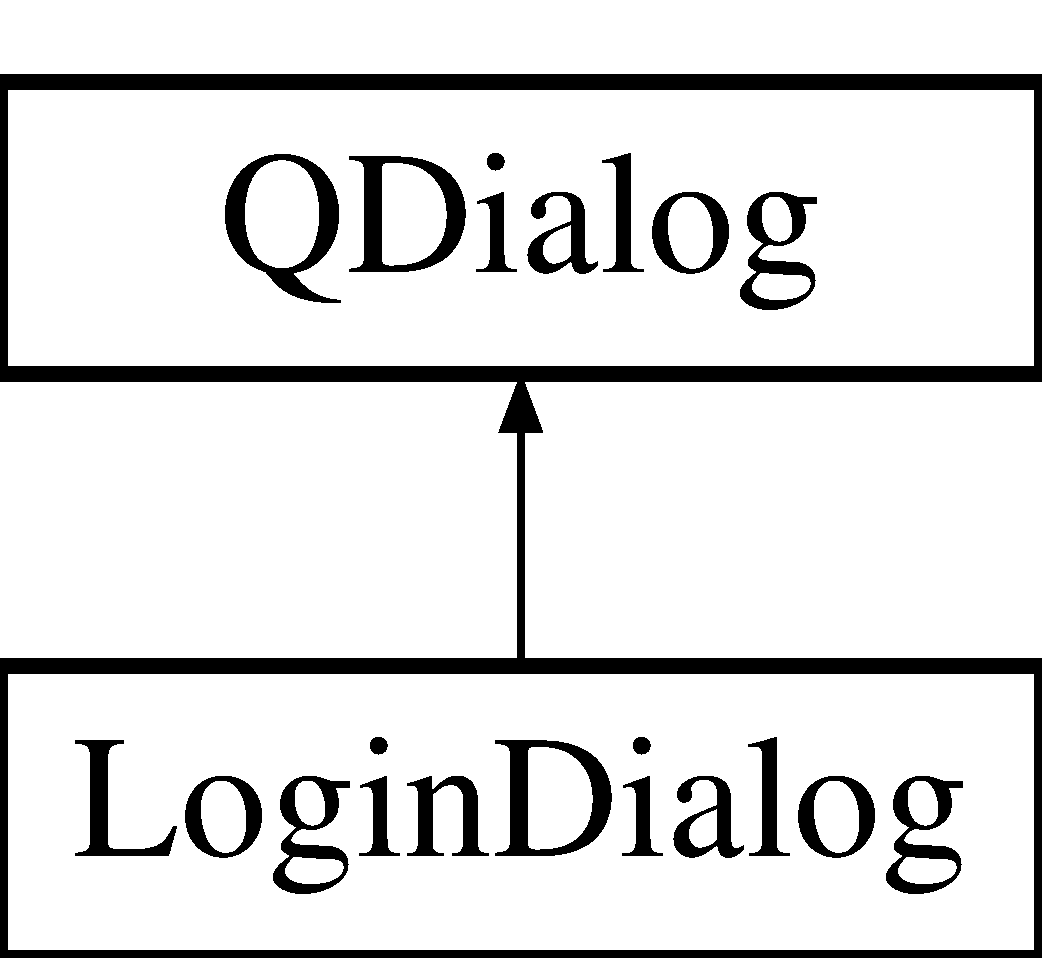
\includegraphics[height=2.000000cm]{classLoginDialog}
\end{center}
\end{figure}
\subsubsection*{Public Member Functions}
\begin{DoxyCompactItemize}
\item 
\mbox{\hyperlink{classLoginDialog_af231bf82d3c72985f62bb47067255f47}{Login\+Dialog}} (Q\+Widget $\ast$parent=0)
\item 
\mbox{\hyperlink{classLoginDialog_aa5d012ebc424713ca0cbd82be1f81133}{$\sim$\+Login\+Dialog}} ()
\item 
void \mbox{\hyperlink{classLoginDialog_a821b2e18f35f4e4d250213a04c4077de}{set\+User\+Names}} (Q\+String\+List names)
\end{DoxyCompactItemize}
\subsubsection*{Public Attributes}
\begin{DoxyCompactItemize}
\item 
Q\+String \mbox{\hyperlink{classLoginDialog_ac3aff74cd5cb23bb5e269775fd7b7672}{user\+Name}}
\item 
Q\+String \mbox{\hyperlink{classLoginDialog_aabe40abeacdb2903b5fa9a61a8562201}{user\+Password}}
\end{DoxyCompactItemize}
\subsubsection*{Protected Member Functions}
\begin{DoxyCompactItemize}
\item 
bool \mbox{\hyperlink{classLoginDialog_a3c1b6041fc659f3f409e129a5c4a7944}{event\+Filter}} (Q\+Object $\ast$watched, Q\+Event $\ast$event)
\item 
void \mbox{\hyperlink{classLoginDialog_a1256114f012018b32b37086f567ffc81}{change\+Event}} (Q\+Event $\ast$event)
\end{DoxyCompactItemize}
\subsubsection*{Private Slots}
\begin{DoxyCompactItemize}
\item 
void \mbox{\hyperlink{classLoginDialog_a7e94645a64f9dd86f7e2bcd6f3dbf7fa}{login\+Accepted}} ()
\end{DoxyCompactItemize}


\subsubsection{Constructor \& Destructor Documentation}
\mbox{\Hypertarget{classLoginDialog_af231bf82d3c72985f62bb47067255f47}\label{classLoginDialog_af231bf82d3c72985f62bb47067255f47}} 
\index{Login\+Dialog@{Login\+Dialog}!Login\+Dialog@{Login\+Dialog}}
\index{Login\+Dialog@{Login\+Dialog}!Login\+Dialog@{Login\+Dialog}}
{\footnotesize\ttfamily Login\+Dialog\+::\texorpdfstring{Login\+Dialog()}{LoginDialog()} (\begin{DoxyParamCaption}\item[{Q\+Widget $\ast$}]{parent = {\ttfamily 0} }\end{DoxyParamCaption})\hspace{0.3cm}{\ttfamily [explicit]}} - standard Q\+Dialog constructor. In constructor connected \textit{p\+Button\+Login} to \hyperlink{classLoginDialog_a7e94645a64f9dd86f7e2bcd6f3dbf7fa}{login\+Accepted}(...) function and installed \hyperlink{classLoginDialog_a3c1b6041fc659f3f409e129a5c4a7944}{event\+Filter} to \textit{line\+Edit\+Password}.

\mbox{\Hypertarget{classLoginDialog_aa5d012ebc424713ca0cbd82be1f81133}\label{classLoginDialog_aa5d012ebc424713ca0cbd82be1f81133}} 
\index{Login\+Dialog@{Login\+Dialog}!````~Login\+Dialog@{$\sim$\+Login\+Dialog}}
\index{````~Login\+Dialog@{$\sim$\+Login\+Dialog}!Login\+Dialog@{Login\+Dialog}}
{\footnotesize\ttfamily Login\+Dialog\+::\texorpdfstring{$\sim$\+Login\+Dialog()}{~LoginDialog()} (\begin{DoxyParamCaption}{ }\end{DoxyParamCaption})} - standard destructor.

\subsubsection{Member Function Documentation}
\mbox{\Hypertarget{classLoginDialog_a1256114f012018b32b37086f567ffc81}\label{classLoginDialog_a1256114f012018b32b37086f567ffc81}} 
\index{Login\+Dialog@{Login\+Dialog}!change\+Event@{change\+Event}}
\index{change\+Event@{change\+Event}!Login\+Dialog@{Login\+Dialog}}
{\footnotesize\ttfamily void Login\+Dialog\+::\texorpdfstring{change\+Event}{changeEvent} (\begin{DoxyParamCaption}\item[{Q\+Event $\ast$}]{event }\end{DoxyParamCaption})\hspace{0.3cm}{\ttfamily [protected]}} - Reimplementation of default event for QWidget to enable user interface translation. Function called automatically.

\mbox{\Hypertarget{classLoginDialog_a3c1b6041fc659f3f409e129a5c4a7944}\label{classLoginDialog_a3c1b6041fc659f3f409e129a5c4a7944}} 
\index{Login\+Dialog@{Login\+Dialog}!event\+Filter@{event\+Filter}}
\index{event\+Filter@{event\+Filter}!Login\+Dialog@{Login\+Dialog}}
{\footnotesize\ttfamily bool Login\+Dialog\+::\texorpdfstring{event\+Filter}{eventFilter} (\begin{DoxyParamCaption}\item[{Q\+Object $\ast$}]{watched,  }\item[{Q\+Event $\ast$}]{event }\end{DoxyParamCaption})\hspace{0.3cm}{\ttfamily [protected]}} - reimplementation of standard function to handle Q\+Event::Mouse\+Button\+Dbl\+Click or Q\+Event::Mouse\+Button\+Release events to call \hyperlink{classKeyboardDialog}{Keyboard\+Dialog} to enter data to
\textit{line\+Edit\+Password}. 

\mbox{\Hypertarget{classLoginDialog_a7e94645a64f9dd86f7e2bcd6f3dbf7fa}\label{classLoginDialog_a7e94645a64f9dd86f7e2bcd6f3dbf7fa}} 
\index{Login\+Dialog@{Login\+Dialog}!login\+Accepted@{login\+Accepted}}
\index{login\+Accepted@{login\+Accepted}!Login\+Dialog@{Login\+Dialog}}
{\footnotesize\ttfamily void Login\+Dialog\+::\texorpdfstring{login\+Accepted}{loginAccepted} (\begin{DoxyParamCaption}{ }\end{DoxyParamCaption})\hspace{0.3cm}{\ttfamily [private]}, {\ttfamily [slot]}} - function which called by \textit{p\+Button\+Login} button and save use name and password to \hyperlink{classLoginDialog_ac3aff74cd5cb23bb5e269775fd7b7672}{user\+Name} and \hyperlink{classLoginDialog_aabe40abeacdb2903b5fa9a61a8562201}{user\+Password} variables and call standard \textit{QDialog::accept()} function to exit from dialog. Parameters \hyperlink{classLoginDialog_ac3aff74cd5cb23bb5e269775fd7b7672}{user\+Name} and \hyperlink{classLoginDialog_aabe40abeacdb2903b5fa9a61a8562201}{user\+Password} are checked in \hyperlink{classMainWindow_a339962b149079e9cdb8928c5528113ea}{user\+Login}(...) function.

\mbox{\Hypertarget{classLoginDialog_a821b2e18f35f4e4d250213a04c4077de}\label{classLoginDialog_a821b2e18f35f4e4d250213a04c4077de}} 
\index{Login\+Dialog@{Login\+Dialog}!set\+User\+Names@{set\+User\+Names}}
\index{set\+User\+Names@{set\+User\+Names}!Login\+Dialog@{Login\+Dialog}}
{\footnotesize\ttfamily void Login\+Dialog\+::\texorpdfstring{set\+User\+Names}{setUserNames} (\begin{DoxyParamCaption}\item[{Q\+String\+List}]{names }\end{DoxyParamCaption})} - function used to fill \textit{listWidget} with \textit{names}. Used to give possibility select user name from list.



\subsubsection{Member Data Documentation}
\mbox{\Hypertarget{classLoginDialog_ac3aff74cd5cb23bb5e269775fd7b7672}\label{classLoginDialog_ac3aff74cd5cb23bb5e269775fd7b7672}} 
\index{Login\+Dialog@{Login\+Dialog}!user\+Name@{user\+Name}}
\index{user\+Name@{user\+Name}!Login\+Dialog@{Login\+Dialog}}
{\footnotesize\ttfamily Q\+String Login\+Dialog\+::\texorpdfstring{user\+Name}{userName}}

\mbox{\Hypertarget{classLoginDialog_aabe40abeacdb2903b5fa9a61a8562201}\label{classLoginDialog_aabe40abeacdb2903b5fa9a61a8562201}} 
\index{Login\+Dialog@{Login\+Dialog}!user\+Password@{user\+Password}}
\index{user\+Password@{user\+Password}!Login\+Dialog@{Login\+Dialog}}
{\footnotesize\ttfamily Q\+String Login\+Dialog\+::\texorpdfstring{user\+Password}{userPassword}}



The documentation for this class was generated from the following files\+:\begin{DoxyCompactItemize}
\item 
\mbox{\hyperlink{logindialog_8h}{logindialog.\+h}}\item 
\mbox{\hyperlink{logindialog_8cpp}{logindialog.\+cpp}}\end{DoxyCompactItemize}
\newpage
\hypertarget{classLogoDialog}{}\subsection{Logo\+Dialog Class Reference}
\label{classLogoDialog}\index{Logo\+Dialog@{Logo\+Dialog}}


{\ttfamily \#include $<$logodialog.\+h$>$}

Inheritance diagram for Logo\+Dialog\+:\begin{figure}[H]
\begin{center}
\leavevmode
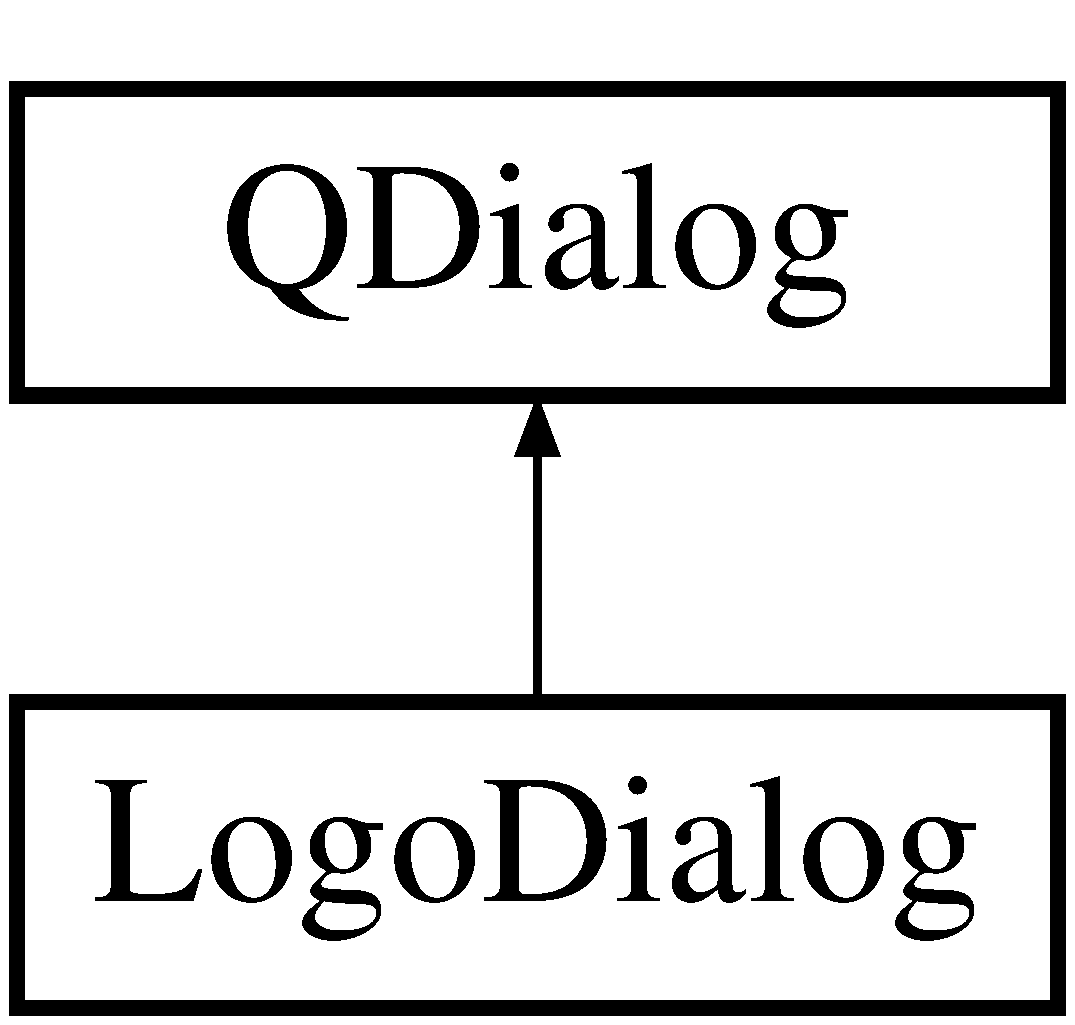
\includegraphics[height=2.000000cm]{classLogoDialog}
\end{center}
\end{figure}
\subsubsection*{Public Member Functions}
\begin{DoxyCompactItemize}
\item 
\mbox{\hyperlink{classLogoDialog_a9457ef5a8c6428bebfa1c56f2d8c9fd1}{Logo\+Dialog}} (Q\+Widget $\ast$parent=0)
\item 
\mbox{\hyperlink{classLogoDialog_a956fbb52cdf488707c5f5a1877727c27}{$\sim$\+Logo\+Dialog}} ()
\end{DoxyCompactItemize}
\subsubsection*{Protected Member Functions}
\begin{DoxyCompactItemize}
\item 
void \mbox{\hyperlink{classLogoDialog_a3c16eea6dbd9e8c50c23444377a9ed12}{show\+Event}} (Q\+Show\+Event $\ast$ev)
\item 
void \mbox{\hyperlink{classLogoDialog_a5d44bdd4d14eed3468e422187ea49a3e}{change\+Event}} (Q\+Event $\ast$event)
\end{DoxyCompactItemize}
\subsubsection*{Private Slots}
\begin{DoxyCompactItemize}
\item 
void \mbox{\hyperlink{classLogoDialog_a7e819a837c81cadaf3cf016b6638b253}{timer\+Time\+Out}} ()
\end{DoxyCompactItemize}
\subsubsection*{Private Attributes}
\begin{DoxyCompactItemize}
\item 
Ui\+::\+Logo\+Dialog $\ast$ \mbox{\hyperlink{classLogoDialog_a4454a373a68ba6473a55dfd404b52e78}{ui}}
\item 
Q\+Timer $\ast$ \mbox{\hyperlink{classLogoDialog_a0f26a533559a0c055ac7ce2ec9d85273}{timer}}
\item 
Q\+Movie $\ast$ \mbox{\hyperlink{classLogoDialog_a45504b8a8b3fc44056859fcb708c2313}{movie}}
\end{DoxyCompactItemize}


\subsubsection{Constructor \& Destructor Documentation}
\mbox{\Hypertarget{classLogoDialog_a9457ef5a8c6428bebfa1c56f2d8c9fd1}\label{classLogoDialog_a9457ef5a8c6428bebfa1c56f2d8c9fd1}} 
\index{Logo\+Dialog@{Logo\+Dialog}!Logo\+Dialog@{Logo\+Dialog}}
\index{Logo\+Dialog@{Logo\+Dialog}!Logo\+Dialog@{Logo\+Dialog}}
{\footnotesize\ttfamily Logo\+Dialog\+::\texorpdfstring{Logo\+Dialog()}{LogoDialog()} (\begin{DoxyParamCaption}\item[{Q\+Widget $\ast$}]{parent = {\ttfamily 0} }\end{DoxyParamCaption})\hspace{0.3cm}{\ttfamily [explicit]}} - standard dialog constructor. At constructor is loading \textit{gif} animation to  \hyperlink{classLogoDialog_a45504b8a8b3fc44056859fcb708c2313}{movie} and creates \hyperlink{classLogoDialog_a0f26a533559a0c055ac7ce2ec9d85273}{timer} which is connected to \hyperlink{classLogoDialog_a7e819a837c81cadaf3cf016b6638b253}{timer\+Time\+Out}(...) function.

\mbox{\Hypertarget{classLogoDialog_a956fbb52cdf488707c5f5a1877727c27}\label{classLogoDialog_a956fbb52cdf488707c5f5a1877727c27}} 
\index{Logo\+Dialog@{Logo\+Dialog}!````~Logo\+Dialog@{$\sim$\+Logo\+Dialog}}
\index{````~Logo\+Dialog@{$\sim$\+Logo\+Dialog}!Logo\+Dialog@{Logo\+Dialog}}
{\footnotesize\ttfamily Logo\+Dialog\+::\texorpdfstring{$\sim$\+Logo\+Dialog()}{~LogoDialog()} (\begin{DoxyParamCaption}{ }\end{DoxyParamCaption})} - standard Q\+Dialog destructor.



\subsubsection{Member Function Documentation}
\mbox{\Hypertarget{classLogoDialog_a5d44bdd4d14eed3468e422187ea49a3e}\label{classLogoDialog_a5d44bdd4d14eed3468e422187ea49a3e}} 
\index{Logo\+Dialog@{Logo\+Dialog}!change\+Event@{change\+Event}}
\index{change\+Event@{change\+Event}!Logo\+Dialog@{Logo\+Dialog}}
{\footnotesize\ttfamily void Logo\+Dialog\+::\texorpdfstring{change\+Event()}{changeEvent()} (\begin{DoxyParamCaption}\item[{Q\+Event $\ast$}]{event }\end{DoxyParamCaption})\hspace{0.3cm}{\ttfamily [protected]}} - reimplementation of default event for QWidget to enable user interface translation. Function called automatically.

\mbox{\Hypertarget{classLogoDialog_a3c16eea6dbd9e8c50c23444377a9ed12}\label{classLogoDialog_a3c16eea6dbd9e8c50c23444377a9ed12}} 
\index{Logo\+Dialog@{Logo\+Dialog}!show\+Event@{show\+Event}}
\index{show\+Event@{show\+Event}!Logo\+Dialog@{Logo\+Dialog}}
{\footnotesize\ttfamily void Logo\+Dialog\+::\texorpdfstring{show\+Event()}{showEvent()} (\begin{DoxyParamCaption}\item[{Q\+Show\+Event $\ast$}]{ev }\end{DoxyParamCaption})\hspace{0.3cm}{\ttfamily [protected]}} - reimplementation of standard Q\+Dialog function. Used to start playing \hyperlink{classLogoDialog_a45504b8a8b3fc44056859fcb708c2313}{movie} and start \hyperlink{classLogoDialog_a0f26a533559a0c055ac7ce2ec9d85273}{timer}.

\mbox{\Hypertarget{classLogoDialog_a7e819a837c81cadaf3cf016b6638b253}\label{classLogoDialog_a7e819a837c81cadaf3cf016b6638b253}} 
\index{Logo\+Dialog@{Logo\+Dialog}!timer\+Time\+Out@{timer\+Time\+Out}}
\index{timer\+Time\+Out@{timer\+Time\+Out}!Logo\+Dialog@{Logo\+Dialog}}
{\footnotesize\ttfamily void Logo\+Dialog\+::\texorpdfstring{timer\+Time\+Out}{timerTimeOut} (\begin{DoxyParamCaption}{ }\end{DoxyParamCaption})\hspace{0.3cm}{\ttfamily [private]}, {\ttfamily [slot]}} - function to close dialog after some count of function calling.



\subsubsection{Member Data Documentation}
\mbox{\Hypertarget{classLogoDialog_a45504b8a8b3fc44056859fcb708c2313}\label{classLogoDialog_a45504b8a8b3fc44056859fcb708c2313}} 
\index{Logo\+Dialog@{Logo\+Dialog}!movie@{movie}}
\index{movie@{movie}!Logo\+Dialog@{Logo\+Dialog}}
{\footnotesize\ttfamily Q\+Movie$\ast$ Logo\+Dialog\+::\texorpdfstring{movie}{movie}\hspace{0.3cm}{\ttfamily [private]}}

\mbox{\Hypertarget{classLogoDialog_a0f26a533559a0c055ac7ce2ec9d85273}\label{classLogoDialog_a0f26a533559a0c055ac7ce2ec9d85273}} 
\index{Logo\+Dialog@{Logo\+Dialog}!timer@{timer}}
\index{timer@{timer}!Logo\+Dialog@{Logo\+Dialog}}
{\footnotesize\ttfamily Q\+Timer$\ast$ Logo\+Dialog\+::\texorpdfstring{timer}{timer}\hspace{0.3cm}{\ttfamily [private]}}

The documentation for this class was generated from the following files\+:\begin{DoxyCompactItemize}
\item 
\mbox{\hyperlink{logodialog_8h}{logodialog.\+h}}\item 
\mbox{\hyperlink{logodialog_8cpp}{logodialog.\+cpp}}\end{DoxyCompactItemize}
\newpage
\hypertarget{unionMachineSettings_1_1MachineHeadType__}{}\subsection{Machine\+Settings\+:\+:Machine\+Head\+Type\+\_\+ Union Reference}
\label{unionMachineSettings_1_1MachineHeadType__}\index{Machine\+Settings\+::\+Machine\+Head\+Type\+\_\+@{Machine\+Settings\+::\+Machine\+Head\+Type\+\_\+}}
Data union for simplify writing data about type of machine.

{\ttfamily \#include $<$settings.\+h$>$}

\subsubsection*{Public Attributes}
\begin{DoxyCompactItemize}
\item 
\begin{tabbing}
xx\=xx\=xx\=xx\=xx\=xx\=xx\=xx\=xx\=\kill
struct \{\\
\>\mbox{\hyperlink{settings_8h_a48091a1e52849b0871df2f7081be2e38}{uint8\_t}} \mbox{\hyperlink{unionMachineSettings_1_1MachineHeadType___afc80a5ddb9d3c32acc2806e3d40b3cac}{servoDriveType}}:3\\
\>\mbox{\hyperlink{settings_8h_a48091a1e52849b0871df2f7081be2e38}{uint8\_t}} \mbox{\hyperlink{unionMachineSettings_1_1MachineHeadType___aa0f8d784533ff6745ba4834918dcd1d0}{carriageType}}:3\\
\>\mbox{\hyperlink{settings_8h_a48091a1e52849b0871df2f7081be2e38}{uint8\_t}} \mbox{\hyperlink{unionMachineSettings_1_1MachineHeadType___a8830b714224e8dcdffe934025ee8b492}{sqFlType}}:2\\
\} \mbox{\hyperlink{unionMachineSettings_1_1MachineHeadType___a3a42ea7e1b8c9424380b826d5156313c}{field}}\\

\end{tabbing}\item 
\mbox{\hyperlink{settings_8h_a48091a1e52849b0871df2f7081be2e38}{uint8\+\_\+t}} \mbox{\hyperlink{unionMachineSettings_1_1MachineHeadType___a739b2ca21cd71e4d27968b8c5168dae7}{all}}
\end{DoxyCompactItemize}


\subsubsection{Member Data Documentation}
\mbox{\Hypertarget{unionMachineSettings_1_1MachineHeadType___a739b2ca21cd71e4d27968b8c5168dae7}\label{unionMachineSettings_1_1MachineHeadType___a739b2ca21cd71e4d27968b8c5168dae7}} 
\index{Machine\+Settings\+::\+Machine\+Head\+Type\+\_\+@{Machine\+Settings\+::\+Machine\+Head\+Type\+\_\+}!all@{all}}
\index{all@{all}!Machine\+Settings\+::\+Machine\+Head\+Type\+\_\+@{Machine\+Settings\+::\+Machine\+Head\+Type\+\_\+}}
{\footnotesize\ttfamily \mbox{\hyperlink{settings_8h_a48091a1e52849b0871df2f7081be2e38}{uint8\+\_\+t}} Machine\+Settings\+::\+Machine\+Head\+Type\+\_\+\+::\texorpdfstring{all}{all}} - variable which contain all bits in one byte in right positions.


\mbox{\Hypertarget{unionMachineSettings_1_1MachineHeadType___a3a42ea7e1b8c9424380b826d5156313c}\label{unionMachineSettings_1_1MachineHeadType___a3a42ea7e1b8c9424380b826d5156313c}} 
\index{Machine\+Settings\+::\+Machine\+Head\+Type\+\_\+@{Machine\+Settings\+::\+Machine\+Head\+Type\+\_\+}!field@{field}}
\index{field@{field}!Machine\+Settings\+::\+Machine\+Head\+Type\+\_\+@{Machine\+Settings\+::\+Machine\+Head\+Type\+\_\+}}
{\footnotesize\ttfamily struct \{ ... \}  Machine\+Settings\+::\+Machine\+Head\+Type\+\_\+\+::\texorpdfstring{field}{field}}

Fields of structure
\begin{DoxyCompactItemize}
\item\mbox{\Hypertarget{unionMachineSettings_1_1MachineHeadType___aa0f8d784533ff6745ba4834918dcd1d0}\label{unionMachineSettings_1_1MachineHeadType___aa0f8d784533ff6745ba4834918dcd1d0}} 
\index{Machine\+Settings\+::\+Machine\+Head\+Type\+\_\+@{Machine\+Settings\+::\+Machine\+Head\+Type\+\_\+}!carriage\+Type@{carriage\+Type}}
\index{carriage\+Type@{carriage\+Type}!Machine\+Settings\+::\+Machine\+Head\+Type\+\_\+@{Machine\+Settings\+::\+Machine\+Head\+Type\+\_\+}}
{\footnotesize\ttfamily \mbox{\hyperlink{settings_8h_a48091a1e52849b0871df2f7081be2e38}{uint8\+\_\+t}} Machine\+Settings\+::\+Machine\+Head\+Type\+\_\+\+::\texorpdfstring{carriage\+Type}{carriageType}}

\item\mbox{\Hypertarget{unionMachineSettings_1_1MachineHeadType___afc80a5ddb9d3c32acc2806e3d40b3cac}\label{unionMachineSettings_1_1MachineHeadType___afc80a5ddb9d3c32acc2806e3d40b3cac}} 
\index{Machine\+Settings\+::\+Machine\+Head\+Type\+\_\+@{Machine\+Settings\+::\+Machine\+Head\+Type\+\_\+}!servo\+Drive\+Type@{servo\+Drive\+Type}}
\index{servo\+Drive\+Type@{servo\+Drive\+Type}!Machine\+Settings\+::\+Machine\+Head\+Type\+\_\+@{Machine\+Settings\+::\+Machine\+Head\+Type\+\_\+}}
{\footnotesize\ttfamily \mbox{\hyperlink{settings_8h_a48091a1e52849b0871df2f7081be2e38}{uint8\+\_\+t}} Machine\+Settings\+::\+Machine\+Head\+Type\+\_\+\+::\texorpdfstring{servo\+Drive\+Type}{servoDriveType}}

\item\mbox{\Hypertarget{unionMachineSettings_1_1MachineHeadType___a8830b714224e8dcdffe934025ee8b492}\label{unionMachineSettings_1_1MachineHeadType___a8830b714224e8dcdffe934025ee8b492}} 
\index{Machine\+Settings\+::\+Machine\+Head\+Type\+\_\+@{Machine\+Settings\+::\+Machine\+Head\+Type\+\_\+}!sq\+Fl\+Type@{sq\+Fl\+Type}}
\index{sq\+Fl\+Type@{sq\+Fl\+Type}!Machine\+Settings\+::\+Machine\+Head\+Type\+\_\+@{Machine\+Settings\+::\+Machine\+Head\+Type\+\_\+}}
{\footnotesize\ttfamily \mbox{\hyperlink{settings_8h_a48091a1e52849b0871df2f7081be2e38}{uint8\+\_\+t}} Machine\+Settings\+::\+Machine\+Head\+Type\+\_\+\+::\texorpdfstring{sq\+Fl\+Type}{sqFlType}}
\end{DoxyCompactItemize}
The documentation for this union was generated from the following file\+:\begin{DoxyCompactItemize}
\item 
\mbox{\hyperlink{settings_8h}{settings.\+h}}\end{DoxyCompactItemize}
\newpage
\hypertarget{unionMachineSettings_1_1MachineIndexLiftType__}{}\subsection{Machine\+Settings\+:\+:Machine\+Index\+Lift\+Type\+\_\+ Union Reference}
\label{unionMachineSettings_1_1MachineIndexLiftType__}\index{Machine\+Settings\+::\+Machine\+Index\+Lift\+Type\+\_\+@{Machine\+Settings\+::\+Machine\+Index\+Lift\+Type\+\_\+}}

Data union for simplify writing data about type of machine.

{\ttfamily \#include $<$settings.\+h$>$}

\subsubsection*{Public Attributes}
\begin{DoxyCompactItemize}
\item 
\begin{tabbing}
xx\=xx\=xx\=xx\=xx\=xx\=xx\=xx\=xx\=\kill
struct \{\\
\>\mbox{\hyperlink{settings_8h_a017dd44e68049ffdd31500a8cd01ba68}{uint16\_t}} \mbox{\hyperlink{unionMachineSettings_1_1MachineIndexLiftType___ade5becd82bf6e7e9a138dd9f338d8eb5}{mainServoDriveType}}:3\\
\>\mbox{\hyperlink{settings_8h_a017dd44e68049ffdd31500a8cd01ba68}{uint16\_t}} \mbox{\hyperlink{unionMachineSettings_1_1MachineIndexLiftType___a3c933bed3921d7e152f6c2695bcd874a}{indexerType}}:3\\
\>\mbox{\hyperlink{settings_8h_a017dd44e68049ffdd31500a8cd01ba68}{uint16\_t}} \mbox{\hyperlink{unionMachineSettings_1_1MachineIndexLiftType___a3966210fa1071db2ed5b38e6dab5df9d}{liftType}}:3\\
\>\mbox{\hyperlink{settings_8h_a017dd44e68049ffdd31500a8cd01ba68}{uint16\_t}} \mbox{\hyperlink{unionMachineSettings_1_1MachineIndexLiftType___ae87b9995b2369b49d0bf1e15ce92221c}{lockType}}:3\\
\>\mbox{\hyperlink{settings_8h_a017dd44e68049ffdd31500a8cd01ba68}{uint16\_t}} \mbox{\hyperlink{unionMachineSettings_1_1MachineIndexLiftType___af18ae62e8274e1ebaf2638ec1d18daba}{hmiIsConnected}}:1\\
\>\mbox{\hyperlink{settings_8h_a017dd44e68049ffdd31500a8cd01ba68}{uint16\_t}} \mbox{\hyperlink{unionMachineSettings_1_1MachineIndexLiftType___a2bce1af1ba728631a1a852008030e753}{keypadIsConnected}}:1\\
\>\mbox{\hyperlink{settings_8h_a017dd44e68049ffdd31500a8cd01ba68}{uint16\_t}} \mbox{\hyperlink{unionMachineSettings_1_1MachineIndexLiftType___a749a9767d0f734e93c11be50db43eb2f}{res\_}}:2\\
\} \mbox{\hyperlink{unionMachineSettings_1_1MachineIndexLiftType___a9e5a66ac224b280a9011c55ecc59fb9e}{field}}\\

\end{tabbing}\item 
\mbox{\hyperlink{settings_8h_a017dd44e68049ffdd31500a8cd01ba68}{uint16\+\_\+t}} \mbox{\hyperlink{unionMachineSettings_1_1MachineIndexLiftType___a0d52f17b3812bed483d864e9b573ef97}{all}}
\end{DoxyCompactItemize}


\subsubsection{Member Data Documentation}
\mbox{\Hypertarget{unionMachineSettings_1_1MachineIndexLiftType___a0d52f17b3812bed483d864e9b573ef97}\label{unionMachineSettings_1_1MachineIndexLiftType___a0d52f17b3812bed483d864e9b573ef97}} 
\index{Machine\+Settings\+::\+Machine\+Index\+Lift\+Type\+\_\+@{Machine\+Settings\+::\+Machine\+Index\+Lift\+Type\+\_\+}!all@{all}}
\index{all@{all}!Machine\+Settings\+::\+Machine\+Index\+Lift\+Type\+\_\+@{Machine\+Settings\+::\+Machine\+Index\+Lift\+Type\+\_\+}}
{\footnotesize\ttfamily \mbox{\hyperlink{settings_8h_a017dd44e68049ffdd31500a8cd01ba68}{uint16\+\_\+t}} Machine\+Settings\+::\+Machine\+Index\+Lift\+Type\+\_\+\+::\texorpdfstring{all}{all}}- variable which contain all bits in one byte in right positions.

\mbox{\Hypertarget{unionMachineSettings_1_1MachineIndexLiftType___a9e5a66ac224b280a9011c55ecc59fb9e}\label{unionMachineSettings_1_1MachineIndexLiftType___a9e5a66ac224b280a9011c55ecc59fb9e}} 
\index{Machine\+Settings\+::\+Machine\+Index\+Lift\+Type\+\_\+@{Machine\+Settings\+::\+Machine\+Index\+Lift\+Type\+\_\+}!field@{field}}
\index{field@{field}!Machine\+Settings\+::\+Machine\+Index\+Lift\+Type\+\_\+@{Machine\+Settings\+::\+Machine\+Index\+Lift\+Type\+\_\+}}
{\footnotesize\ttfamily struct \{ ... \}  Machine\+Settings\+::\+Machine\+Index\+Lift\+Type\+\_\+\+::\texorpdfstring{field}{field}}

Fields of structure.
\begin{DoxyCompactItemize}
\item\mbox{\Hypertarget{unionMachineSettings_1_1MachineIndexLiftType___af18ae62e8274e1ebaf2638ec1d18daba}\label{unionMachineSettings_1_1MachineIndexLiftType___af18ae62e8274e1ebaf2638ec1d18daba}} 
\index{Machine\+Settings\+::\+Machine\+Index\+Lift\+Type\+\_\+@{Machine\+Settings\+::\+Machine\+Index\+Lift\+Type\+\_\+}!hmi\+Is\+Connected@{hmi\+Is\+Connected}}
\index{hmi\+Is\+Connected@{hmi\+Is\+Connected}!Machine\+Settings\+::\+Machine\+Index\+Lift\+Type\+\_\+@{Machine\+Settings\+::\+Machine\+Index\+Lift\+Type\+\_\+}}
{\footnotesize\ttfamily \mbox{\hyperlink{settings_8h_a017dd44e68049ffdd31500a8cd01ba68}{uint16\+\_\+t}} Machine\+Settings\+::\+Machine\+Index\+Lift\+Type\+\_\+\+::\texorpdfstring{hmi\+Is\+Connected}{hmiIsConnected}}

\item\mbox{\Hypertarget{unionMachineSettings_1_1MachineIndexLiftType___a3c933bed3921d7e152f6c2695bcd874a}\label{unionMachineSettings_1_1MachineIndexLiftType___a3c933bed3921d7e152f6c2695bcd874a}} 
\index{Machine\+Settings\+::\+Machine\+Index\+Lift\+Type\+\_\+@{Machine\+Settings\+::\+Machine\+Index\+Lift\+Type\+\_\+}!indexer\+Type@{indexer\+Type}}
\index{indexer\+Type@{indexer\+Type}!Machine\+Settings\+::\+Machine\+Index\+Lift\+Type\+\_\+@{Machine\+Settings\+::\+Machine\+Index\+Lift\+Type\+\_\+}}
{\footnotesize\ttfamily \mbox{\hyperlink{settings_8h_a017dd44e68049ffdd31500a8cd01ba68}{uint16\+\_\+t}} Machine\+Settings\+::\+Machine\+Index\+Lift\+Type\+\_\+\+::\texorpdfstring{indexer\+Type}{indexerType}}

\item\mbox{\Hypertarget{unionMachineSettings_1_1MachineIndexLiftType___a2bce1af1ba728631a1a852008030e753}\label{unionMachineSettings_1_1MachineIndexLiftType___a2bce1af1ba728631a1a852008030e753}} 
\index{Machine\+Settings\+::\+Machine\+Index\+Lift\+Type\+\_\+@{Machine\+Settings\+::\+Machine\+Index\+Lift\+Type\+\_\+}!keypad\+Is\+Connected@{keypad\+Is\+Connected}}
\index{keypad\+Is\+Connected@{keypad\+Is\+Connected}!Machine\+Settings\+::\+Machine\+Index\+Lift\+Type\+\_\+@{Machine\+Settings\+::\+Machine\+Index\+Lift\+Type\+\_\+}}
{\footnotesize\ttfamily \mbox{\hyperlink{settings_8h_a017dd44e68049ffdd31500a8cd01ba68}{uint16\+\_\+t}} Machine\+Settings\+::\+Machine\+Index\+Lift\+Type\+\_\+\+::\texorpdfstring{keypad\+Is\+Connected}{keypadIsConnected}}

\item\mbox{\Hypertarget{unionMachineSettings_1_1MachineIndexLiftType___a3966210fa1071db2ed5b38e6dab5df9d}\label{unionMachineSettings_1_1MachineIndexLiftType___a3966210fa1071db2ed5b38e6dab5df9d}} 
\index{Machine\+Settings\+::\+Machine\+Index\+Lift\+Type\+\_\+@{Machine\+Settings\+::\+Machine\+Index\+Lift\+Type\+\_\+}!lift\+Type@{lift\+Type}}
\index{lift\+Type@{lift\+Type}!Machine\+Settings\+::\+Machine\+Index\+Lift\+Type\+\_\+@{Machine\+Settings\+::\+Machine\+Index\+Lift\+Type\+\_\+}}
{\footnotesize\ttfamily \mbox{\hyperlink{settings_8h_a017dd44e68049ffdd31500a8cd01ba68}{uint16\+\_\+t}} Machine\+Settings\+::\+Machine\+Index\+Lift\+Type\+\_\+\+::\texorpdfstring{lift\+Type}{liftType}}

\item\mbox{\Hypertarget{unionMachineSettings_1_1MachineIndexLiftType___ae87b9995b2369b49d0bf1e15ce92221c}\label{unionMachineSettings_1_1MachineIndexLiftType___ae87b9995b2369b49d0bf1e15ce92221c}} 
\index{Machine\+Settings\+::\+Machine\+Index\+Lift\+Type\+\_\+@{Machine\+Settings\+::\+Machine\+Index\+Lift\+Type\+\_\+}!lock\+Type@{lock\+Type}}
\index{lock\+Type@{lock\+Type}!Machine\+Settings\+::\+Machine\+Index\+Lift\+Type\+\_\+@{Machine\+Settings\+::\+Machine\+Index\+Lift\+Type\+\_\+}}
{\footnotesize\ttfamily \mbox{\hyperlink{settings_8h_a017dd44e68049ffdd31500a8cd01ba68}{uint16\+\_\+t}} Machine\+Settings\+::\+Machine\+Index\+Lift\+Type\+\_\+\+::\texorpdfstring{lock\+Type}{lockType}}

\item\mbox{\Hypertarget{unionMachineSettings_1_1MachineIndexLiftType___ade5becd82bf6e7e9a138dd9f338d8eb5}\label{unionMachineSettings_1_1MachineIndexLiftType___ade5becd82bf6e7e9a138dd9f338d8eb5}} 
\index{Machine\+Settings\+::\+Machine\+Index\+Lift\+Type\+\_\+@{Machine\+Settings\+::\+Machine\+Index\+Lift\+Type\+\_\+}!main\+Servo\+Drive\+Type@{main\+Servo\+Drive\+Type}}
\index{main\+Servo\+Drive\+Type@{main\+Servo\+Drive\+Type}!Machine\+Settings\+::\+Machine\+Index\+Lift\+Type\+\_\+@{Machine\+Settings\+::\+Machine\+Index\+Lift\+Type\+\_\+}}
{\footnotesize\ttfamily \mbox{\hyperlink{settings_8h_a017dd44e68049ffdd31500a8cd01ba68}{uint16\+\_\+t}} Machine\+Settings\+::\+Machine\+Index\+Lift\+Type\+\_\+\+::\texorpdfstring{main\+Servo\+Drive\+Type}{mainServoDriveType}}
\end{DoxyCompactItemize}

\mbox{\Hypertarget{unionMachineSettings_1_1MachineIndexLiftType___a749a9767d0f734e93c11be50db43eb2f}\label{unionMachineSettings_1_1MachineIndexLiftType___a749a9767d0f734e93c11be50db43eb2f}} 
\index{Machine\+Settings\+::\+Machine\+Index\+Lift\+Type\+\_\+@{Machine\+Settings\+::\+Machine\+Index\+Lift\+Type\+\_\+}!res\+\_\+@{res\+\_\+}}
\index{res\+\_\+@{res\+\_\+}!Machine\+Settings\+::\+Machine\+Index\+Lift\+Type\+\_\+@{Machine\+Settings\+::\+Machine\+Index\+Lift\+Type\+\_\+}}
{\footnotesize\ttfamily \mbox{\hyperlink{settings_8h_a017dd44e68049ffdd31500a8cd01ba68}{uint16\+\_\+t}} Machine\+Settings\+::\+Machine\+Index\+Lift\+Type\+\_\+\+::\texorpdfstring{res\+\_\+}{res\_}} - reserved bits.



The documentation for this union was generated from the following file\+:\begin{DoxyCompactItemize}
\item 
\mbox{\hyperlink{settings_8h}{settings.\+h}}\end{DoxyCompactItemize}
\newpage
\hypertarget{structMachineSettings_1_1MachineParameters__}{}\subsection{Machine\+Settings\+:\+:Machine\+Parameters\+\_\+ Struct Reference}
\label{structMachineSettings_1_1MachineParameters__}\index{Machine\+Settings\+::\+Machine\+Parameters\+\_\+@{Machine\+Settings\+::\+Machine\+Parameters\+\_\+}}


{\ttfamily \#include $<$settings.\+h$>$}

\subsubsection*{Public Member Functions}
\begin{DoxyCompactItemize}
\item 
Q\+Byte\+Array \mbox{\hyperlink{structMachineSettings_1_1MachineParameters___a7c9a7fa5df12c0dcfa7747025c99cf3d}{to\+Byte\+Array}} ()
\end{DoxyCompactItemize}
\subsubsection*{Public Attributes}
\begin{DoxyCompactItemize}
\item 
\mbox{\hyperlink{settings_8h_a017dd44e68049ffdd31500a8cd01ba68}{uint16\+\_\+t}} \mbox{\hyperlink{structMachineSettings_1_1MachineParameters___a1234db3781ecb40815e39f2526f7811e}{head\+Count}}
\item 
\mbox{\hyperlink{settings_8h_a017dd44e68049ffdd31500a8cd01ba68}{uint16\+\_\+t}} \mbox{\hyperlink{structMachineSettings_1_1MachineParameters___a768a1b74bc3572a9c750dc6bec224721}{warning\+Time}}
\item 
int16\+\_\+t \mbox{\hyperlink{structMachineSettings_1_1MachineParameters___ae1cf9b5025c05ca6f1b0f6e60a52ae94}{direction}}
\item 
\mbox{\hyperlink{classMachineSettings_af95330ff3a80de06fe956f5297ec0fc5}{Machine\+Type}} \mbox{\hyperlink{structMachineSettings_1_1MachineParameters___a912fbcf6b92c4e46502cbe324d01c703}{machine\+Type}}
\item 
\mbox{\hyperlink{classMachineSettings_ab7b6a5e7f8a67169e7c28067e7d4bbe9}{Machine\+Head\+Type}} \mbox{\hyperlink{structMachineSettings_1_1MachineParameters___a49482960d30282f4a2145b0dda8e5966}{head\+Type}}
\item 
\mbox{\hyperlink{classMachineSettings_a0a3b23271b2f401ab585236bd8330a82}{Machine\+Index\+Lift\+Type}} \mbox{\hyperlink{structMachineSettings_1_1MachineParameters___ac0753e42ecb5bdeee9d14878042baba3}{indexe\+Lift\+Type}}
\item 
\mbox{\hyperlink{settings_8h_a017dd44e68049ffdd31500a8cd01ba68}{uint16\+\_\+t}} \mbox{\hyperlink{structMachineSettings_1_1MachineParameters___a670e405c759be710e76ff9587aeb3b36}{head\+Max\+Range}}
\item 
\mbox{\hyperlink{settings_8h_a017dd44e68049ffdd31500a8cd01ba68}{uint16\+\_\+t}} \mbox{\hyperlink{structMachineSettings_1_1MachineParameters___a1b3146b3f2731d091ef6aae3332f6db7}{lift\+Gear\+Ratio}}
\item 
\mbox{\hyperlink{settings_8h_a017dd44e68049ffdd31500a8cd01ba68}{uint16\+\_\+t}} \mbox{\hyperlink{structMachineSettings_1_1MachineParameters___aba437f9a48c61521df2bc63e5fbe1afc}{indexer\+Screw\+Pinch}}
\item 
\mbox{\hyperlink{settings_8h_a48091a1e52849b0871df2f7081be2e38}{uint8\+\_\+t}} \mbox{\hyperlink{structMachineSettings_1_1MachineParameters___a9e49eb233cef299776a6da0bc5c1ee60}{use\+Unload\+Head}}
\item 
\mbox{\hyperlink{settings_8h_a48091a1e52849b0871df2f7081be2e38}{uint8\+\_\+t}} \mbox{\hyperlink{structMachineSettings_1_1MachineParameters___afd73ad9d9a7eb0a787d5357eaf28d751}{step\+Time\+Delay}}
\item 
\mbox{\hyperlink{classMachineSettings_ad31cf583a3d6462e47d920209239ffe6}{Last\+Revolver\+Warm}} \mbox{\hyperlink{structMachineSettings_1_1MachineParameters___aa257ad2a6e209c00bc4d6e24277ad8ed}{last\+Rev\+Warm}}
\end{DoxyCompactItemize}


\subsubsection{Member Function Documentation}
\mbox{\Hypertarget{structMachineSettings_1_1MachineParameters___a7c9a7fa5df12c0dcfa7747025c99cf3d}\label{structMachineSettings_1_1MachineParameters___a7c9a7fa5df12c0dcfa7747025c99cf3d}} 
\index{Machine\+Settings\+::\+Machine\+Parameters\+\_\+@{Machine\+Settings\+::\+Machine\+Parameters\+\_\+}!to\+Byte\+Array@{to\+Byte\+Array}}
\index{to\+Byte\+Array@{to\+Byte\+Array}!Machine\+Settings\+::\+Machine\+Parameters\+\_\+@{Machine\+Settings\+::\+Machine\+Parameters\+\_\+}}
{\footnotesize\ttfamily Q\+Byte\+Array Machine\+Settings\+::\+Machine\+Parameters\+\_\+\+::\texorpdfstring{to\+Byte\+Array}{toByteArray} (\begin{DoxyParamCaption}{ }\end{DoxyParamCaption})} - function to gather all structure items to Q\+Byte\+Array to have possibility save data on hard drive in compact format.



\subsubsection{Member Data Documentation}
\mbox{\Hypertarget{structMachineSettings_1_1MachineParameters___ae1cf9b5025c05ca6f1b0f6e60a52ae94}\label{structMachineSettings_1_1MachineParameters___ae1cf9b5025c05ca6f1b0f6e60a52ae94}} 
\index{Machine\+Settings\+::\+Machine\+Parameters\+\_\+@{Machine\+Settings\+::\+Machine\+Parameters\+\_\+}!direction@{direction}}
\index{direction@{direction}!Machine\+Settings\+::\+Machine\+Parameters\+\_\+@{Machine\+Settings\+::\+Machine\+Parameters\+\_\+}}
{\footnotesize\ttfamily int16\+\_\+t Machine\+Settings\+::\+Machine\+Parameters\+\_\+\+::\texorpdfstring{direction}{direction}}

\mbox{\Hypertarget{structMachineSettings_1_1MachineParameters___a1234db3781ecb40815e39f2526f7811e}\label{structMachineSettings_1_1MachineParameters___a1234db3781ecb40815e39f2526f7811e}} 
\index{Machine\+Settings\+::\+Machine\+Parameters\+\_\+@{Machine\+Settings\+::\+Machine\+Parameters\+\_\+}!head\+Count@{head\+Count}}
\index{head\+Count@{head\+Count}!Machine\+Settings\+::\+Machine\+Parameters\+\_\+@{Machine\+Settings\+::\+Machine\+Parameters\+\_\+}}
{\footnotesize\ttfamily \mbox{\hyperlink{settings_8h_a017dd44e68049ffdd31500a8cd01ba68}{uint16\+\_\+t}} Machine\+Settings\+::\+Machine\+Parameters\+\_\+\+::\texorpdfstring{head\+Count}{headCount}}

\mbox{\Hypertarget{structMachineSettings_1_1MachineParameters___a670e405c759be710e76ff9587aeb3b36}\label{structMachineSettings_1_1MachineParameters___a670e405c759be710e76ff9587aeb3b36}} 
\index{Machine\+Settings\+::\+Machine\+Parameters\+\_\+@{Machine\+Settings\+::\+Machine\+Parameters\+\_\+}!head\+Max\+Range@{head\+Max\+Range}}
\index{head\+Max\+Range@{head\+Max\+Range}!Machine\+Settings\+::\+Machine\+Parameters\+\_\+@{Machine\+Settings\+::\+Machine\+Parameters\+\_\+}}
{\footnotesize\ttfamily \mbox{\hyperlink{settings_8h_a017dd44e68049ffdd31500a8cd01ba68}{uint16\+\_\+t}} Machine\+Settings\+::\+Machine\+Parameters\+\_\+\+::\texorpdfstring{head\+Max\+Range}{headMaxRange}}

\mbox{\Hypertarget{structMachineSettings_1_1MachineParameters___a49482960d30282f4a2145b0dda8e5966}\label{structMachineSettings_1_1MachineParameters___a49482960d30282f4a2145b0dda8e5966}} 
\index{Machine\+Settings\+::\+Machine\+Parameters\+\_\+@{Machine\+Settings\+::\+Machine\+Parameters\+\_\+}!head\+Type@{head\+Type}}
\index{head\+Type@{head\+Type}!Machine\+Settings\+::\+Machine\+Parameters\+\_\+@{Machine\+Settings\+::\+Machine\+Parameters\+\_\+}}
{\footnotesize\ttfamily \mbox{\hyperlink{classMachineSettings_ab7b6a5e7f8a67169e7c28067e7d4bbe9}{Machine\+Head\+Type}} Machine\+Settings\+::\+Machine\+Parameters\+\_\+\+::\texorpdfstring{head\+Type}{headType}}

\mbox{\Hypertarget{structMachineSettings_1_1MachineParameters___ac0753e42ecb5bdeee9d14878042baba3}\label{structMachineSettings_1_1MachineParameters___ac0753e42ecb5bdeee9d14878042baba3}} 
\index{Machine\+Settings\+::\+Machine\+Parameters\+\_\+@{Machine\+Settings\+::\+Machine\+Parameters\+\_\+}!indexe\+Lift\+Type@{indexe\+Lift\+Type}}
\index{indexe\+Lift\+Type@{indexe\+Lift\+Type}!Machine\+Settings\+::\+Machine\+Parameters\+\_\+@{Machine\+Settings\+::\+Machine\+Parameters\+\_\+}}
{\footnotesize\ttfamily \mbox{\hyperlink{classMachineSettings_a0a3b23271b2f401ab585236bd8330a82}{Machine\+Index\+Lift\+Type}} Machine\+Settings\+::\+Machine\+Parameters\+\_\+\+::\texorpdfstring{indexe\+Lift\+Type}{indexeLiftType}}

\mbox{\Hypertarget{structMachineSettings_1_1MachineParameters___aba437f9a48c61521df2bc63e5fbe1afc}\label{structMachineSettings_1_1MachineParameters___aba437f9a48c61521df2bc63e5fbe1afc}} 
\index{Machine\+Settings\+::\+Machine\+Parameters\+\_\+@{Machine\+Settings\+::\+Machine\+Parameters\+\_\+}!indexer\+Screw\+Pinch@{indexer\+Screw\+Pinch}}
\index{indexer\+Screw\+Pinch@{indexer\+Screw\+Pinch}!Machine\+Settings\+::\+Machine\+Parameters\+\_\+@{Machine\+Settings\+::\+Machine\+Parameters\+\_\+}}
{\footnotesize\ttfamily \mbox{\hyperlink{settings_8h_a017dd44e68049ffdd31500a8cd01ba68}{uint16\+\_\+t}} Machine\+Settings\+::\+Machine\+Parameters\+\_\+\+::\texorpdfstring{indexer\+Screw\+Pinch}{indexerScrewPinch}}

\mbox{\Hypertarget{structMachineSettings_1_1MachineParameters___aa257ad2a6e209c00bc4d6e24277ad8ed}\label{structMachineSettings_1_1MachineParameters___aa257ad2a6e209c00bc4d6e24277ad8ed}} 
\index{Machine\+Settings\+::\+Machine\+Parameters\+\_\+@{Machine\+Settings\+::\+Machine\+Parameters\+\_\+}!last\+Rev\+Warm@{last\+Rev\+Warm}}
\index{last\+Rev\+Warm@{last\+Rev\+Warm}!Machine\+Settings\+::\+Machine\+Parameters\+\_\+@{Machine\+Settings\+::\+Machine\+Parameters\+\_\+}}
{\footnotesize\ttfamily \mbox{\hyperlink{classMachineSettings_ad31cf583a3d6462e47d920209239ffe6}{Last\+Revolver\+Warm}} Machine\+Settings\+::\+Machine\+Parameters\+\_\+\+::\texorpdfstring{last\+Rev\+Warm}{lastRevWarm}}

\mbox{\Hypertarget{structMachineSettings_1_1MachineParameters___a1b3146b3f2731d091ef6aae3332f6db7}\label{structMachineSettings_1_1MachineParameters___a1b3146b3f2731d091ef6aae3332f6db7}} 
\index{Machine\+Settings\+::\+Machine\+Parameters\+\_\+@{Machine\+Settings\+::\+Machine\+Parameters\+\_\+}!lift\+Gear\+Ratio@{lift\+Gear\+Ratio}}
\index{lift\+Gear\+Ratio@{lift\+Gear\+Ratio}!Machine\+Settings\+::\+Machine\+Parameters\+\_\+@{Machine\+Settings\+::\+Machine\+Parameters\+\_\+}}
{\footnotesize\ttfamily \mbox{\hyperlink{settings_8h_a017dd44e68049ffdd31500a8cd01ba68}{uint16\+\_\+t}} Machine\+Settings\+::\+Machine\+Parameters\+\_\+\+::\texorpdfstring{lift\+Gear\+Ratio}{liftGearRatio}}

\mbox{\Hypertarget{structMachineSettings_1_1MachineParameters___a912fbcf6b92c4e46502cbe324d01c703}\label{structMachineSettings_1_1MachineParameters___a912fbcf6b92c4e46502cbe324d01c703}} 
\index{Machine\+Settings\+::\+Machine\+Parameters\+\_\+@{Machine\+Settings\+::\+Machine\+Parameters\+\_\+}!machine\+Type@{machine\+Type}}
\index{machine\+Type@{machine\+Type}!Machine\+Settings\+::\+Machine\+Parameters\+\_\+@{Machine\+Settings\+::\+Machine\+Parameters\+\_\+}}
{\footnotesize\ttfamily \mbox{\hyperlink{classMachineSettings_af95330ff3a80de06fe956f5297ec0fc5}{Machine\+Type}} Machine\+Settings\+::\+Machine\+Parameters\+\_\+\+::\texorpdfstring{machine\+Type}{machineType}}

\mbox{\Hypertarget{structMachineSettings_1_1MachineParameters___afd73ad9d9a7eb0a787d5357eaf28d751}\label{structMachineSettings_1_1MachineParameters___afd73ad9d9a7eb0a787d5357eaf28d751}} 
\index{Machine\+Settings\+::\+Machine\+Parameters\+\_\+@{Machine\+Settings\+::\+Machine\+Parameters\+\_\+}!step\+Time\+Delay@{step\+Time\+Delay}}
\index{step\+Time\+Delay@{step\+Time\+Delay}!Machine\+Settings\+::\+Machine\+Parameters\+\_\+@{Machine\+Settings\+::\+Machine\+Parameters\+\_\+}}
{\footnotesize\ttfamily \mbox{\hyperlink{settings_8h_a48091a1e52849b0871df2f7081be2e38}{uint8\+\_\+t}} Machine\+Settings\+::\+Machine\+Parameters\+\_\+\+::\texorpdfstring{step\+Time\+Delay}{stepTimeDelay}}

\mbox{\Hypertarget{structMachineSettings_1_1MachineParameters___a9e49eb233cef299776a6da0bc5c1ee60}\label{structMachineSettings_1_1MachineParameters___a9e49eb233cef299776a6da0bc5c1ee60}} 
\index{Machine\+Settings\+::\+Machine\+Parameters\+\_\+@{Machine\+Settings\+::\+Machine\+Parameters\+\_\+}!use\+Unload\+Head@{use\+Unload\+Head}}
\index{use\+Unload\+Head@{use\+Unload\+Head}!Machine\+Settings\+::\+Machine\+Parameters\+\_\+@{Machine\+Settings\+::\+Machine\+Parameters\+\_\+}}
{\footnotesize\ttfamily \mbox{\hyperlink{settings_8h_a48091a1e52849b0871df2f7081be2e38}{uint8\+\_\+t}} Machine\+Settings\+::\+Machine\+Parameters\+\_\+\+::\texorpdfstring{use\+Unload\+Head}{useUnloadHead}}

\mbox{\Hypertarget{structMachineSettings_1_1MachineParameters___a768a1b74bc3572a9c750dc6bec224721}\label{structMachineSettings_1_1MachineParameters___a768a1b74bc3572a9c750dc6bec224721}} 
\index{Machine\+Settings\+::\+Machine\+Parameters\+\_\+@{Machine\+Settings\+::\+Machine\+Parameters\+\_\+}!warning\+Time@{warning\+Time}}
\index{warning\+Time@{warning\+Time}!Machine\+Settings\+::\+Machine\+Parameters\+\_\+@{Machine\+Settings\+::\+Machine\+Parameters\+\_\+}}
{\footnotesize\ttfamily \mbox{\hyperlink{settings_8h_a017dd44e68049ffdd31500a8cd01ba68}{uint16\+\_\+t}} Machine\+Settings\+::\+Machine\+Parameters\+\_\+\+::\texorpdfstring{warning\+Time}{warningTime}}



The documentation for this struct was generated from the following files\+:\begin{DoxyCompactItemize}
\item 
\mbox{\hyperlink{settings_8h}{settings.\+h}}\item 
\mbox{\hyperlink{settings_8cpp}{settings.\+cpp}}\end{DoxyCompactItemize}
\newpage
\hypertarget{classMachineSettings}{}\subsection{Machine\+Settings Class Reference}
\label{classMachineSettings}\index{Machine\+Settings@{Machine\+Settings}}


{\ttfamily \#include $<$settings.\+h$>$}

\subsubsection*{Classes}
\begin{DoxyCompactItemize}
\item 
union \mbox{\hyperlink{unionMachineSettings_1_1LastRevolverWarm__}{Last\+Revolver\+Warm\+\_\+}}
\item 
union \mbox{\hyperlink{unionMachineSettings_1_1MachineHeadType__}{Machine\+Head\+Type\+\_\+}}
\item 
union \mbox{\hyperlink{unionMachineSettings_1_1MachineIndexLiftType__}{Machine\+Index\+Lift\+Type\+\_\+}}
\item 
struct \mbox{\hyperlink{structMachineSettings_1_1MachineParameters__}{Machine\+Parameters\+\_\+}}
\item 
union \mbox{\hyperlink{unionMachineSettings_1_1MachineState__}{Machine\+State\+\_\+}}
\end{DoxyCompactItemize}
\subsubsection*{Public Types}
\begin{DoxyCompactItemize}
\item 
enum \mbox{\hyperlink{classMachineSettings_ace5f0a84d32c0423bb62f068f102bf80}{Devices}} \{ \mbox{\hyperlink{classMachineSettings_ace5f0a84d32c0423bb62f068f102bf80aa0ef1af1f748dd75f12dd479a07ff628}{Master\+Device}} = 0x0000
 \}
\item 
enum \mbox{\hyperlink{classMachineSettings_a81ac5b64df7f302bae854ee794f9fbef}{Master\+Data\+Places}} \{ 
\begin{DoxyCompactItemize}
\item\mbox{\hyperlink{classMachineSettings_a81ac5b64df7f302bae854ee794f9fbefa5b952989bf58820434feab7ec0f0e84f}{Master\+Head\+Count}} = 0x0001, 
\item\mbox{\hyperlink{classMachineSettings_a81ac5b64df7f302bae854ee794f9fbefa60c8ac4e12ef5ac9ecd807711ca296c3}{Master\+Last\+Button}} = 0x0003, 
\item\mbox{\hyperlink{classMachineSettings_a81ac5b64df7f302bae854ee794f9fbefad8ee6c0fdfad3e9effda8056da5e68a8}{Master\+Index\+Lift\+Command}} = 0x0004, 
\item\mbox{\hyperlink{classMachineSettings_a81ac5b64df7f302bae854ee794f9fbefa03ad3d79f6edfe1a2477748d6a66386e}{Master\+Head\+State\+Lo}} = 0x0005, 
\item\mbox{\hyperlink{classMachineSettings_a81ac5b64df7f302bae854ee794f9fbefa76129cc9720d12f63764b4089d638589}{Master\+Head\+State\+Hi}} = 0x0009, 
\item\mbox{\hyperlink{classMachineSettings_a81ac5b64df7f302bae854ee794f9fbefabc28c130aa7c10b12f97486f6d443b66}{Master\+Palet\+State\+Lo}} = 0x000A, 
\item\mbox{\hyperlink{classMachineSettings_a81ac5b64df7f302bae854ee794f9fbefaf61a688c14b1370c4630e7bacac34771}{Master\+Palet\+State\+Hi}} = 0x0012, 
\item\mbox{\hyperlink{classMachineSettings_a81ac5b64df7f302bae854ee794f9fbefaf1538a4ff7b63f627657f5fc722a6d25}{Master\+Machine\+Type}} = 0x0011
\end{DoxyCompactItemize}
 \}
\item 
enum \mbox{\hyperlink{classMachineSettings_a0feee7a1964811bb4a602e9cc3bf459f}{Machine\+Type\+\_\+}} \{ 
\begin{DoxyCompactItemize}
\item\mbox{\hyperlink{classMachineSettings_a0feee7a1964811bb4a602e9cc3bf459fa90d1454dea114dab1be411c61eb2506f}{Volt\+Servo}} = 0x0000, 
\item\mbox{\hyperlink{classMachineSettings_a0feee7a1964811bb4a602e9cc3bf459facb1903efc2ca403d2b8bafad23ac475a}{Volt\+AC}}, 
\item\mbox{\hyperlink{classMachineSettings_a0feee7a1964811bb4a602e9cc3bf459fabbded889bc90d83b77be39316591c3e7}{Vector}}, 
\item\mbox{\hyperlink{classMachineSettings_a0feee7a1964811bb4a602e9cc3bf459faabaa3c9e55c4ed04fbf1f544bbaf2ee3}{Titan\+A\+SE}}, 
\item\mbox{\hyperlink{classMachineSettings_a0feee7a1964811bb4a602e9cc3bf459fadc58b3fd25459977198f34e19e63c49a}{Titan\+A\+SA}}, 
\item\mbox{\hyperlink{classMachineSettings_a0feee7a1964811bb4a602e9cc3bf459faddbd23233dca7bda197b435fedff8344}{Titan\+A\+AA}}
\end{DoxyCompactItemize}
 \}
\item 
typedef union \mbox{\hyperlink{unionMachineSettings_1_1MachineState__}{Machine\+Settings\+::\+Machine\+State\+\_\+}} \mbox{\hyperlink{classMachineSettings_a3d02f0565ba9c53dbb59d5d086208cad}{Machine\+State}}
\item 
typedef enum \mbox{\hyperlink{classMachineSettings_a0feee7a1964811bb4a602e9cc3bf459f}{Machine\+Settings\+::\+Machine\+Type\+\_\+}} \mbox{\hyperlink{classMachineSettings_af95330ff3a80de06fe956f5297ec0fc5}{Machine\+Type}}
\item 
typedef union \mbox{\hyperlink{unionMachineSettings_1_1MachineHeadType__}{Machine\+Settings\+::\+Machine\+Head\+Type\+\_\+}} \mbox{\hyperlink{classMachineSettings_ab7b6a5e7f8a67169e7c28067e7d4bbe9}{Machine\+Head\+Type}}
\item 
typedef union \mbox{\hyperlink{unionMachineSettings_1_1MachineIndexLiftType__}{Machine\+Settings\+::\+Machine\+Index\+Lift\+Type\+\_\+}} \mbox{\hyperlink{classMachineSettings_a0a3b23271b2f401ab585236bd8330a82}{Machine\+Index\+Lift\+Type}}
\item 
typedef union \mbox{\hyperlink{unionMachineSettings_1_1LastRevolverWarm__}{Machine\+Settings\+::\+Last\+Revolver\+Warm\+\_\+}} \mbox{\hyperlink{classMachineSettings_ad31cf583a3d6462e47d920209239ffe6}{Last\+Revolver\+Warm}}
\item 
typedef struct \mbox{\hyperlink{structMachineSettings_1_1MachineParameters__}{Machine\+Settings\+::\+Machine\+Parameters\+\_\+}} \mbox{\hyperlink{classMachineSettings_a87879e13793dbc7c10d4fa18e1236751}{Machine\+Parameters}}
\end{DoxyCompactItemize}
\subsubsection*{Public Member Functions}
\begin{DoxyCompactItemize}
\item 
\mbox{\hyperlink{classMachineSettings_ab1b5f2057a07bb5bf20931cd9d5afb25}{Machine\+Settings}} (\mbox{\hyperlink{classMachineSettings_a87879e13793dbc7c10d4fa18e1236751}{Machine\+Parameters}} m\+Param)
\item 
\mbox{\hyperlink{classMachineSettings_a6ecb0fe6e75f5c33941cb08d467e834f}{Machine\+Settings}} ()
\item 
void \mbox{\hyperlink{classMachineSettings_ac28b9c28855fe22c85e95379eea9c252}{from\+Byte\+Array}} (Q\+Byte\+Array machine\+Param\+Array)
\end{DoxyCompactItemize}
\subsubsection*{Static Public Member Functions}
\begin{DoxyCompactItemize}
\item 
static bool \mbox{\hyperlink{classMachineSettings_aed23d5dfd20513c309956d187e0b7a3b}{get\+Service\+Widg\+En}} ()
\item 
static void \mbox{\hyperlink{classMachineSettings_a849f1eefa33684d98531d4052b9923e1}{set\+Service\+Widg\+En}} (bool serv\+En)
\item 
static \mbox{\hyperlink{classMachineSettings_af95330ff3a80de06fe956f5297ec0fc5}{Machine\+Type}} \mbox{\hyperlink{classMachineSettings_a0349f2cb52c9359909722942a831aeae}{get\+Machine\+Type}} ()
\item 
static void \mbox{\hyperlink{classMachineSettings_aba8aeb52eef51e98eedb65a52d22ab0f}{set\+Machine\+Type}} (\mbox{\hyperlink{classMachineSettings_af95330ff3a80de06fe956f5297ec0fc5}{Machine\+Type}} m\+Type)
\item 
static bool \mbox{\hyperlink{classMachineSettings_a232ca3eed7f64a1721e23f1bf3ad9243}{get\+Machine\+Idle}} ()
\item 
static void \mbox{\hyperlink{classMachineSettings_a81d10b1a8eef770d08c22df5796dbd8b}{set\+Machine\+Idle}} (bool idle)
\item 
static \mbox{\hyperlink{settings_8h_a017dd44e68049ffdd31500a8cd01ba68}{uint16\+\_\+t}} \mbox{\hyperlink{classMachineSettings_a77384a60e0ded049aa4c4a5c0b5e193b}{get\+Head\+Max\+Range}} ()
\item 
static \mbox{\hyperlink{settings_8h_a017dd44e68049ffdd31500a8cd01ba68}{uint16\+\_\+t}} \mbox{\hyperlink{classMachineSettings_a806a1562aea709bb99a614485ee5401e}{get\+Head\+Type}} ()
\item 
static \mbox{\hyperlink{settings_8h_a017dd44e68049ffdd31500a8cd01ba68}{uint16\+\_\+t}} \mbox{\hyperlink{classMachineSettings_acb8ca9e673941dd7abb8c429e9525f2a}{get\+Index\+Lift\+Type}} ()
\item 
static \mbox{\hyperlink{settings_8h_a017dd44e68049ffdd31500a8cd01ba68}{uint16\+\_\+t}} \mbox{\hyperlink{classMachineSettings_a8b0acb6f0ad4a795c8ea18338c035e14}{get\+Head\+Pal\+State\+Lo}} ()
\item 
static \mbox{\hyperlink{settings_8h_a017dd44e68049ffdd31500a8cd01ba68}{uint16\+\_\+t}} \mbox{\hyperlink{classMachineSettings_aca60698179b068072b45bea26c919da9}{get\+Head\+Pal\+State\+Hi}} ()
\item 
static void \mbox{\hyperlink{classMachineSettings_a5ec4d87fc0832c6b79d5229085237252}{set\+Head\+Max\+Range}} (\mbox{\hyperlink{settings_8h_a017dd44e68049ffdd31500a8cd01ba68}{uint16\+\_\+t}} val)
\item 
static void \mbox{\hyperlink{classMachineSettings_a33f6697feb74cab98d582f80bd4dd6a2}{set\+Head\+Type}} (\mbox{\hyperlink{settings_8h_a017dd44e68049ffdd31500a8cd01ba68}{uint16\+\_\+t}} val)
\item 
static void \mbox{\hyperlink{classMachineSettings_a546ae7011ac82ecf38125c2ba534d327}{set\+Index\+Lift\+Type}} (\mbox{\hyperlink{settings_8h_a017dd44e68049ffdd31500a8cd01ba68}{uint16\+\_\+t}} val)
\item 
static void \mbox{\hyperlink{classMachineSettings_ad1db42477cae871db33526bf828dd6a7}{set\+Head\+Pal\+State\+Lo}} (\mbox{\hyperlink{settings_8h_a017dd44e68049ffdd31500a8cd01ba68}{uint16\+\_\+t}} val)
\item 
static void \mbox{\hyperlink{classMachineSettings_a8b1fe308c75ea1bafd283e0f97b87a93}{set\+Head\+Pal\+State\+Hi}} (\mbox{\hyperlink{settings_8h_a017dd44e68049ffdd31500a8cd01ba68}{uint16\+\_\+t}} val)
\item 
static void \mbox{\hyperlink{classMachineSettings_aa568893fe06e0bc946dc7ceb33535aaa}{set\+Head\+Pal\+State\+Index}} (int index, bool state)
\end{DoxyCompactItemize}
\subsubsection*{Public Attributes}
\begin{DoxyCompactItemize}
\item 
Q\+String\+List \mbox{\hyperlink{classMachineSettings_ad0e371856a610c685f0cde9f9cb2b5c5}{machine\+Type\+List}}
\item 
Q\+List$<$ int $>$ \mbox{\hyperlink{classMachineSettings_abe0a0868f7081db78076e61fd8793384}{machine\+Type\+Data}}
\item 
\mbox{\hyperlink{classMachineSettings_a87879e13793dbc7c10d4fa18e1236751}{Machine\+Parameters}} \mbox{\hyperlink{classMachineSettings_abca1961654d6dd586ec26990e5d49ed7}{machine\+Param}}
\end{DoxyCompactItemize}
\subsubsection*{Static Public Attributes}
\begin{DoxyCompactItemize}
\item 
static bool \mbox{\hyperlink{classMachineSettings_a9a8e6bc0e09fa8ac8e32e30cbbd5ef4c}{service\+Widgets\+En}}
\item 
static \mbox{\hyperlink{classMachineSettings_af95330ff3a80de06fe956f5297ec0fc5}{Machine\+Type}} \mbox{\hyperlink{classMachineSettings_ae3167629c7a8723b123ff5616fb284af}{machine\+Type\+Stat}}
\item 
static bool \mbox{\hyperlink{classMachineSettings_a8297d5ccf01292708bc4aae65180a54c}{machine\+Idle}}
\end{DoxyCompactItemize}
\subsubsection*{Static Private Attributes}
\begin{DoxyCompactItemize}
\item 
static \mbox{\hyperlink{settings_8h_a017dd44e68049ffdd31500a8cd01ba68}{uint16\+\_\+t}} \mbox{\hyperlink{classMachineSettings_ab223e2bea0de3ab0c85452d124d2b434}{head\+Max\+Range\+Stat}}
\item 
static \mbox{\hyperlink{settings_8h_a017dd44e68049ffdd31500a8cd01ba68}{uint16\+\_\+t}} \mbox{\hyperlink{classMachineSettings_a1cfa5a234b9cbce7c1e1b881992e1d2e}{head\+Type\+Stat}}
\item 
static \mbox{\hyperlink{settings_8h_a017dd44e68049ffdd31500a8cd01ba68}{uint16\+\_\+t}} \mbox{\hyperlink{classMachineSettings_a358c9d4ed568f50c5279c7019c97ffc2}{indexer\+Lift\+Type\+Stat}}
\item 
static \mbox{\hyperlink{settings_8h_a4196118492a3b1493c81f250e90af775}{uint32\+\_\+t}} \mbox{\hyperlink{classMachineSettings_a1543a985ca7e47a2853dcfef75227a5a}{head\+Pal\+State\+Stat}}
\end{DoxyCompactItemize}


\subsubsection{Member Typedef Documentation}
\mbox{\Hypertarget{classMachineSettings_ad31cf583a3d6462e47d920209239ffe6}\label{classMachineSettings_ad31cf583a3d6462e47d920209239ffe6}} 
\index{Machine\+Settings@{Machine\+Settings}!Last\+Revolver\+Warm@{Last\+Revolver\+Warm}}
\index{Last\+Revolver\+Warm@{Last\+Revolver\+Warm}!Machine\+Settings@{Machine\+Settings}}
{\footnotesize\ttfamily typedef union \mbox{\hyperlink{unionMachineSettings_1_1LastRevolverWarm__}{Machine\+Settings\+::\+Last\+Revolver\+Warm\+\_\+}} \mbox{\hyperlink{classMachineSettings_ad31cf583a3d6462e47d920209239ffe6}{Machine\+Settings\+::\texorpdfstring{Last\+Revolver\+Warm}{LastRevolverWarm}}}} - union of data fields to write to \hyperlink{structRegister_1_1IndexerReg___1_1reg_a9b0063135d16e0ea6f47284c361bfb03}{indexer\+Reg\+\_\+\+TM} by parameters names.

\mbox{\Hypertarget{classMachineSettings_ab7b6a5e7f8a67169e7c28067e7d4bbe9}\label{classMachineSettings_ab7b6a5e7f8a67169e7c28067e7d4bbe9}} 
\index{Machine\+Settings@{Machine\+Settings}!Machine\+Head\+Type@{Machine\+Head\+Type}}
\index{Machine\+Head\+Type@{Machine\+Head\+Type}!Machine\+Settings@{Machine\+Settings}}
{\footnotesize\ttfamily typedef union \mbox{\hyperlink{unionMachineSettings_1_1MachineHeadType__}{Machine\+Settings\+::\+Machine\+Head\+Type\+\_\+}} \mbox{\hyperlink{classMachineSettings_ab7b6a5e7f8a67169e7c28067e7d4bbe9}{Machine\+Settings\+::\texorpdfstring{Machine\+Head\+Type}{MachineHeadType}}}} - union of data to declare parameters of head.

\mbox{\Hypertarget{classMachineSettings_a0a3b23271b2f401ab585236bd8330a82}\label{classMachineSettings_a0a3b23271b2f401ab585236bd8330a82}} 
\index{Machine\+Settings@{Machine\+Settings}!Machine\+Index\+Lift\+Type@{Machine\+Index\+Lift\+Type}}
\index{Machine\+Index\+Lift\+Type@{Machine\+Index\+Lift\+Type}!Machine\+Settings@{Machine\+Settings}}
{\footnotesize\ttfamily typedef union \mbox{\hyperlink{unionMachineSettings_1_1MachineIndexLiftType__}{Machine\+Settings\+::\+Machine\+Index\+Lift\+Type\+\_\+}} \mbox{\hyperlink{classMachineSettings_a0a3b23271b2f401ab585236bd8330a82}{Machine\+Settings\+::\texorpdfstring{Machine\+Index\+Lift\+Type}{MachineIndexLiftType}}}} - union of data to declare parameters of lift.

\mbox{\Hypertarget{classMachineSettings_a87879e13793dbc7c10d4fa18e1236751}\label{classMachineSettings_a87879e13793dbc7c10d4fa18e1236751}} 
\index{Machine\+Settings@{Machine\+Settings}!Machine\+Parameters@{Machine\+Parameters}}
\index{Machine\+Parameters@{Machine\+Parameters}!Machine\+Settings@{Machine\+Settings}}
{\footnotesize\ttfamily typedef struct \mbox{\hyperlink{structMachineSettings_1_1MachineParameters__}{Machine\+Settings\+::\+Machine\+Parameters\+\_\+}} \mbox{\hyperlink{classMachineSettings_a87879e13793dbc7c10d4fa18e1236751}{Machine\+Settings\+::\texorpdfstring{Machine\+Parameters}{MachineParameters}}}} - structure  of data to save machine parameters to save it on hard drive.

\mbox{\Hypertarget{classMachineSettings_a3d02f0565ba9c53dbb59d5d086208cad}\label{classMachineSettings_a3d02f0565ba9c53dbb59d5d086208cad}} 
\index{Machine\+Settings@{Machine\+Settings}!Machine\+State@{Machine\+State}}
\index{Machine\+State@{Machine\+State}!Machine\+Settings@{Machine\+Settings}}
{\footnotesize\ttfamily typedef union \mbox{\hyperlink{unionMachineSettings_1_1MachineState__}{Machine\+Settings\+::\+Machine\+State\+\_\+}} \mbox{\hyperlink{classMachineSettings_a3d02f0565ba9c53dbb59d5d086208cad}{Machine\+Settings\+::\texorpdfstring{Machine\+State}{MachineState}}}} - union to save state of machine to use in program.

\mbox{\Hypertarget{classMachineSettings_af95330ff3a80de06fe956f5297ec0fc5}\label{classMachineSettings_af95330ff3a80de06fe956f5297ec0fc5}} 
\index{Machine\+Settings@{Machine\+Settings}!Machine\+Type@{Machine\+Type}}
\index{Machine\+Type@{Machine\+Type}!Machine\+Settings@{Machine\+Settings}}
{\footnotesize\ttfamily typedef enum \mbox{\hyperlink{classMachineSettings_a0feee7a1964811bb4a602e9cc3bf459f}{Machine\+Settings\+::\+Machine\+Type\+\_\+}} \mbox{\hyperlink{classMachineSettings_af95330ff3a80de06fe956f5297ec0fc5}{Machine\+Settings\+::\texorpdfstring{Machine\+Type}{MachineType}}}} - enumerator to save type of machine to hide or show widgets on dialogs.

\subsubsection{Member Enumeration Documentation}
\mbox{\Hypertarget{classMachineSettings_ace5f0a84d32c0423bb62f068f102bf80}\label{classMachineSettings_ace5f0a84d32c0423bb62f068f102bf80}} 
\index{Machine\+Settings@{Machine\+Settings}!Devices@{Devices}}
\index{Devices@{Devices}!Machine\+Settings@{Machine\+Settings}}
{\footnotesize\ttfamily enum \mbox{\hyperlink{classMachineSettings_ace5f0a84d32c0423bb62f068f102bf80}{Machine\+Settings\+::\texorpdfstring{Devices}{Devices}}}} - enumerator to declare address of devices to send data to appropriated fields.

\begin{DoxyEnumFields}{Enumerator}
\raisebox{\heightof{T}}[0pt][0pt]{\index{Master\+Device@{Master\+Device}!Machine\+Settings@{Machine\+Settings}}\index{Machine\+Settings@{Machine\+Settings}!Master\+Device@{Master\+Device}}}\mbox{\Hypertarget{classMachineSettings_ace5f0a84d32c0423bb62f068f102bf80aa0ef1af1f748dd75f12dd479a07ff628}\label{classMachineSettings_ace5f0a84d32c0423bb62f068f102bf80aa0ef1af1f748dd75f12dd479a07ff628}} 
Master\+Device&0x0000\\
\hline

\end{DoxyEnumFields}
\mbox{\Hypertarget{classMachineSettings_a0feee7a1964811bb4a602e9cc3bf459f}\label{classMachineSettings_a0feee7a1964811bb4a602e9cc3bf459f}} 
\index{Machine\+Settings@{Machine\+Settings}!Machine\+Type\+\_\+@{Machine\+Type\+\_\+}}
\index{Machine\+Type\+\_\+@{Machine\+Type\+\_\+}!Machine\+Settings@{Machine\+Settings}}
{\footnotesize\ttfamily enum \mbox{\hyperlink{classMachineSettings_a0feee7a1964811bb4a602e9cc3bf459f}{Machine\+Settings\+::\texorpdfstring{Machine\+Type\+\_\+}{MachineType\_}}}}

\begin{DoxyEnumFields}{Enumerator}
\raisebox{\heightof{T}}[0pt][0pt]{\index{Volt\+Servo@{Volt\+Servo}!Machine\+Settings@{Machine\+Settings}}\index{Machine\+Settings@{Machine\+Settings}!Volt\+Servo@{Volt\+Servo}}}\mbox{\Hypertarget{classMachineSettings_a0feee7a1964811bb4a602e9cc3bf459fa90d1454dea114dab1be411c61eb2506f}\label{classMachineSettings_a0feee7a1964811bb4a602e9cc3bf459fa90d1454dea114dab1be411c61eb2506f}} 
Volt\+Servo&0x0000\\
\hline

\raisebox{\heightof{T}}[0pt][0pt]{\index{Volt\+AC@{Volt\+AC}!Machine\+Settings@{Machine\+Settings}}\index{Machine\+Settings@{Machine\+Settings}!Volt\+AC@{Volt\+AC}}}\mbox{\Hypertarget{classMachineSettings_a0feee7a1964811bb4a602e9cc3bf459facb1903efc2ca403d2b8bafad23ac475a}\label{classMachineSettings_a0feee7a1964811bb4a602e9cc3bf459facb1903efc2ca403d2b8bafad23ac475a}} 
Volt\+AC&0x0001\\
\hline

\raisebox{\heightof{T}}[0pt][0pt]{\index{Vector@{Vector}!Machine\+Settings@{Machine\+Settings}}\index{Machine\+Settings@{Machine\+Settings}!Vector@{Vector}}}\mbox{\Hypertarget{classMachineSettings_a0feee7a1964811bb4a602e9cc3bf459fabbded889bc90d83b77be39316591c3e7}\label{classMachineSettings_a0feee7a1964811bb4a602e9cc3bf459fabbded889bc90d83b77be39316591c3e7}} 
Vector&0x0002\\
\hline

\raisebox{\heightof{T}}[0pt][0pt]{\index{Titan\+A\+SE@{Titan\+A\+SE}!Machine\+Settings@{Machine\+Settings}}\index{Machine\+Settings@{Machine\+Settings}!Titan\+A\+SE@{Titan\+A\+SE}}}\mbox{\Hypertarget{classMachineSettings_a0feee7a1964811bb4a602e9cc3bf459faabaa3c9e55c4ed04fbf1f544bbaf2ee3}\label{classMachineSettings_a0feee7a1964811bb4a602e9cc3bf459faabaa3c9e55c4ed04fbf1f544bbaf2ee3}} 
Titan\+A\+SE&0x0003\\
\hline

\raisebox{\heightof{T}}[0pt][0pt]{\index{Titan\+A\+SA@{Titan\+A\+SA}!Machine\+Settings@{Machine\+Settings}}\index{Machine\+Settings@{Machine\+Settings}!Titan\+A\+SA@{Titan\+A\+SA}}}\mbox{\Hypertarget{classMachineSettings_a0feee7a1964811bb4a602e9cc3bf459fadc58b3fd25459977198f34e19e63c49a}\label{classMachineSettings_a0feee7a1964811bb4a602e9cc3bf459fadc58b3fd25459977198f34e19e63c49a}} 
Titan\+A\+SA&0x0004\\
\hline

\raisebox{\heightof{T}}[0pt][0pt]{\index{Titan\+A\+AA@{Titan\+A\+AA}!Machine\+Settings@{Machine\+Settings}}\index{Machine\+Settings@{Machine\+Settings}!Titan\+A\+AA@{Titan\+A\+AA}}}\mbox{\Hypertarget{classMachineSettings_a0feee7a1964811bb4a602e9cc3bf459faddbd23233dca7bda197b435fedff8344}\label{classMachineSettings_a0feee7a1964811bb4a602e9cc3bf459faddbd23233dca7bda197b435fedff8344}} 
Titan\+A\+AA&0x0005\\
\hline

\end{DoxyEnumFields}
\mbox{\Hypertarget{classMachineSettings_a81ac5b64df7f302bae854ee794f9fbef}\label{classMachineSettings_a81ac5b64df7f302bae854ee794f9fbef}} 
\index{Machine\+Settings@{Machine\+Settings}!Master\+Data\+Places@{Master\+Data\+Places}}
\index{Master\+Data\+Places@{Master\+Data\+Places}!Machine\+Settings@{Machine\+Settings}}
{\footnotesize\ttfamily enum \mbox{\hyperlink{classMachineSettings_a81ac5b64df7f302bae854ee794f9fbef}{Machine\+Settings\+::\texorpdfstring{Master\+Data\+Places}{MasterDataPlaces}}}}

\begin{DoxyEnumFields}{Enumerator}
\raisebox{\heightof{T}}[0pt][0pt]{\index{Master\+Head\+Count@{Master\+Head\+Count}!Machine\+Settings@{Machine\+Settings}}\index{Machine\+Settings@{Machine\+Settings}!Master\+Head\+Count@{Master\+Head\+Count}}}\mbox{\Hypertarget{classMachineSettings_a81ac5b64df7f302bae854ee794f9fbefa5b952989bf58820434feab7ec0f0e84f}\label{classMachineSettings_a81ac5b64df7f302bae854ee794f9fbefa5b952989bf58820434feab7ec0f0e84f}} 
Master\+Head\+Count&0x0001\\
\hline

\raisebox{\heightof{T}}[0pt][0pt]{\index{Master\+Last\+Button@{Master\+Last\+Button}!Machine\+Settings@{Machine\+Settings}}\index{Machine\+Settings@{Machine\+Settings}!Master\+Last\+Button@{Master\+Last\+Button}}}\mbox{\Hypertarget{classMachineSettings_a81ac5b64df7f302bae854ee794f9fbefa60c8ac4e12ef5ac9ecd807711ca296c3}\label{classMachineSettings_a81ac5b64df7f302bae854ee794f9fbefa60c8ac4e12ef5ac9ecd807711ca296c3}} 
Master\+Last\+Button&0x0003\\
\hline

\raisebox{\heightof{T}}[0pt][0pt]{\index{Master\+Index\+Lift\+Command@{Master\+Index\+Lift\+Command}!Machine\+Settings@{Machine\+Settings}}\index{Machine\+Settings@{Machine\+Settings}!Master\+Index\+Lift\+Command@{Master\+Index\+Lift\+Command}}}\mbox{\Hypertarget{classMachineSettings_a81ac5b64df7f302bae854ee794f9fbefad8ee6c0fdfad3e9effda8056da5e68a8}\label{classMachineSettings_a81ac5b64df7f302bae854ee794f9fbefad8ee6c0fdfad3e9effda8056da5e68a8}} 
Master\+Index\+Lift\+Command&0x0004\\
\hline

\raisebox{\heightof{T}}[0pt][0pt]{\index{Master\+Head\+State\+Lo@{Master\+Head\+State\+Lo}!Machine\+Settings@{Machine\+Settings}}\index{Machine\+Settings@{Machine\+Settings}!Master\+Head\+State\+Lo@{Master\+Head\+State\+Lo}}}\mbox{\Hypertarget{classMachineSettings_a81ac5b64df7f302bae854ee794f9fbefa03ad3d79f6edfe1a2477748d6a66386e}\label{classMachineSettings_a81ac5b64df7f302bae854ee794f9fbefa03ad3d79f6edfe1a2477748d6a66386e}} 
Master\+Head\+State\+Lo&0x0005\\
\hline

\raisebox{\heightof{T}}[0pt][0pt]{\index{Master\+Head\+State\+Hi@{Master\+Head\+State\+Hi}!Machine\+Settings@{Machine\+Settings}}\index{Machine\+Settings@{Machine\+Settings}!Master\+Head\+State\+Hi@{Master\+Head\+State\+Hi}}}\mbox{\Hypertarget{classMachineSettings_a81ac5b64df7f302bae854ee794f9fbefa76129cc9720d12f63764b4089d638589}\label{classMachineSettings_a81ac5b64df7f302bae854ee794f9fbefa76129cc9720d12f63764b4089d638589}} 
Master\+Head\+State\+Hi&0x0009\\
\hline

\raisebox{\heightof{T}}[0pt][0pt]{\index{Master\+Palet\+State\+Lo@{Master\+Palet\+State\+Lo}!Machine\+Settings@{Machine\+Settings}}\index{Machine\+Settings@{Machine\+Settings}!Master\+Palet\+State\+Lo@{Master\+Palet\+State\+Lo}}}\mbox{\Hypertarget{classMachineSettings_a81ac5b64df7f302bae854ee794f9fbefabc28c130aa7c10b12f97486f6d443b66}\label{classMachineSettings_a81ac5b64df7f302bae854ee794f9fbefabc28c130aa7c10b12f97486f6d443b66}} 
Master\+Palet\+State\+Lo&0x000A\\
\hline

\raisebox{\heightof{T}}[0pt][0pt]{\index{Master\+Palet\+State\+Hi@{Master\+Palet\+State\+Hi}!Machine\+Settings@{Machine\+Settings}}\index{Machine\+Settings@{Machine\+Settings}!Master\+Palet\+State\+Hi@{Master\+Palet\+State\+Hi}}}\mbox{\Hypertarget{classMachineSettings_a81ac5b64df7f302bae854ee794f9fbefaf61a688c14b1370c4630e7bacac34771}\label{classMachineSettings_a81ac5b64df7f302bae854ee794f9fbefaf61a688c14b1370c4630e7bacac34771}} 
Master\+Palet\+State\+Hi&0x0012\\
\hline

\raisebox{\heightof{T}}[0pt][0pt]{\index{Master\+Machine\+Type@{Master\+Machine\+Type}!Machine\+Settings@{Machine\+Settings}}\index{Machine\+Settings@{Machine\+Settings}!Master\+Machine\+Type@{Master\+Machine\+Type}}}\mbox{\Hypertarget{classMachineSettings_a81ac5b64df7f302bae854ee794f9fbefaf1538a4ff7b63f627657f5fc722a6d25}\label{classMachineSettings_a81ac5b64df7f302bae854ee794f9fbefaf1538a4ff7b63f627657f5fc722a6d25}} 
Master\+Machine\+Type&0x0011\\
\hline

\end{DoxyEnumFields}


\subsubsection{Constructor \& Destructor Documentation}
\mbox{\Hypertarget{classMachineSettings_ab1b5f2057a07bb5bf20931cd9d5afb25}\label{classMachineSettings_ab1b5f2057a07bb5bf20931cd9d5afb25}} 
\index{Machine\+Settings@{Machine\+Settings}!Machine\+Settings@{Machine\+Settings}}
\index{Machine\+Settings@{Machine\+Settings}!Machine\+Settings@{Machine\+Settings}}
{\footnotesize\ttfamily Machine\+Settings\+::\texorpdfstring{Machine\+Settings}{MachineSettings}{\footnotesize\ttfamily [1/2]} (\begin{DoxyParamCaption}\item[{\mbox{\hyperlink{classMachineSettings_a87879e13793dbc7c10d4fa18e1236751}{Machine\+Settings\+::\+Machine\+Parameters}}}]{m\+Param }\end{DoxyParamCaption})} - constructor of class to initialize fields of structure with given in \textit{mParam} variable parameters. 

\mbox{\Hypertarget{classMachineSettings_a6ecb0fe6e75f5c33941cb08d467e834f}\label{classMachineSettings_a6ecb0fe6e75f5c33941cb08d467e834f}} 
\index{Machine\+Settings@{Machine\+Settings}!Machine\+Settings@{Machine\+Settings}}
\index{Machine\+Settings@{Machine\+Settings}!Machine\+Settings@{Machine\+Settings}}
{\footnotesize\ttfamily Machine\+Settings\+::\texorpdfstring{Machine\+Settings}{MachineSettings}{\footnotesize\ttfamily [2/2]} (\begin{DoxyParamCaption}{ }\end{DoxyParamCaption})} - constructor of class to initialize fields of structure with default parameters.

\subsubsection{Member Function Documentation}
\mbox{\Hypertarget{classMachineSettings_ac28b9c28855fe22c85e95379eea9c252}\label{classMachineSettings_ac28b9c28855fe22c85e95379eea9c252}} 
\index{Machine\+Settings@{Machine\+Settings}!from\+Byte\+Array@{from\+Byte\+Array}}
\index{from\+Byte\+Array@{from\+Byte\+Array}!Machine\+Settings@{Machine\+Settings}}
{\footnotesize\ttfamily void Machine\+Settings\+::\texorpdfstring{from\+Byte\+Array}{fromByteArray} (\begin{DoxyParamCaption}\item[{Q\+Byte\+Array}]{machine\+Param\+Array }\end{DoxyParamCaption})} - function to fill appropriated fields of class with data given in \textit{machine\+Param\+Array}

\mbox{\Hypertarget{classMachineSettings_a77384a60e0ded049aa4c4a5c0b5e193b}\label{classMachineSettings_a77384a60e0ded049aa4c4a5c0b5e193b}} 
\index{Machine\+Settings@{Machine\+Settings}!get\+Head\+Max\+Range@{get\+Head\+Max\+Range}}
\index{get\+Head\+Max\+Range@{get\+Head\+Max\+Range}!Machine\+Settings@{Machine\+Settings}}
{\footnotesize\ttfamily \mbox{\hyperlink{settings_8h_a017dd44e68049ffdd31500a8cd01ba68}{uint16\+\_\+t}} Machine\+Settings\+::\texorpdfstring{get\+Head\+Max\+Range}{getHeadMaxRange} (\begin{DoxyParamCaption}{ }\end{DoxyParamCaption}){\ttfamily [static]}} - function to get value of \hyperlink{classMachineSettings_ab223e2bea0de3ab0c85452d124d2b434}{head\+Max\+Range\+Stat} variable.

\mbox{\Hypertarget{classMachineSettings_aca60698179b068072b45bea26c919da9}\label{classMachineSettings_aca60698179b068072b45bea26c919da9}} 
\index{Machine\+Settings@{Machine\+Settings}!get\+Head\+Pal\+State\+Hi@{get\+Head\+Pal\+State\+Hi}}
\index{get\+Head\+Pal\+State\+Hi@{get\+Head\+Pal\+State\+Hi}!Machine\+Settings@{Machine\+Settings}}
{\footnotesize\ttfamily \mbox{\hyperlink{settings_8h_a017dd44e68049ffdd31500a8cd01ba68}{uint16\+\_\+t}} Machine\+Settings\+::\texorpdfstring{get\+Head\+Pal\+State\+Hi}{getHeadPalStateHi} (\begin{DoxyParamCaption}{ }\end{DoxyParamCaption}){\ttfamily [static]}} - function to get highest 16 bit of \hyperlink{classMachineSettings_a1543a985ca7e47a2853dcfef75227a5a}{head\+Pal\+State\+Stat} variable.

\mbox{\Hypertarget{classMachineSettings_a8b0acb6f0ad4a795c8ea18338c035e14}\label{classMachineSettings_a8b0acb6f0ad4a795c8ea18338c035e14}} 
\index{Machine\+Settings@{Machine\+Settings}!get\+Head\+Pal\+State\+Lo@{get\+Head\+Pal\+State\+Lo}}
\index{get\+Head\+Pal\+State\+Lo@{get\+Head\+Pal\+State\+Lo}!Machine\+Settings@{Machine\+Settings}}
{\footnotesize\ttfamily \mbox{\hyperlink{settings_8h_a017dd44e68049ffdd31500a8cd01ba68}{uint16\+\_\+t}} Machine\+Settings\+::\texorpdfstring{get\+Head\+Pal\+State\+Lo}{getHeadPalStateLo} (\begin{DoxyParamCaption}{ }\end{DoxyParamCaption}){\ttfamily [static]}} - function to get lowest 16 bit of \hyperlink{classMachineSettings_a1543a985ca7e47a2853dcfef75227a5a}{head\+Pal\+State\+Stat} variable.

\mbox{\Hypertarget{classMachineSettings_a806a1562aea709bb99a614485ee5401e}\label{classMachineSettings_a806a1562aea709bb99a614485ee5401e}} 
\index{Machine\+Settings@{Machine\+Settings}!get\+Head\+Type@{get\+Head\+Type}}
\index{get\+Head\+Type@{get\+Head\+Type}!Machine\+Settings@{Machine\+Settings}}
{\footnotesize\ttfamily \mbox{\hyperlink{settings_8h_a017dd44e68049ffdd31500a8cd01ba68}{uint16\+\_\+t}} Machine\+Settings\+::\texorpdfstring{get\+Head\+Type}{getHeadType} (\begin{DoxyParamCaption}{ }\end{DoxyParamCaption}){\ttfamily [static]}} - function to get value of \hyperlink{classMachineSettings_a1cfa5a234b9cbce7c1e1b881992e1d2e}{head\+Type\+Stat} variable.

\mbox{\Hypertarget{classMachineSettings_acb8ca9e673941dd7abb8c429e9525f2a}\label{classMachineSettings_acb8ca9e673941dd7abb8c429e9525f2a}} 
\index{Machine\+Settings@{Machine\+Settings}!get\+Index\+Lift\+Type@{get\+Index\+Lift\+Type}}
\index{get\+Index\+Lift\+Type@{get\+Index\+Lift\+Type}!Machine\+Settings@{Machine\+Settings}}
{\footnotesize\ttfamily \mbox{\hyperlink{settings_8h_a017dd44e68049ffdd31500a8cd01ba68}{uint16\+\_\+t}} Machine\+Settings\+::\texorpdfstring{get\+Index\+Lift\+Type}{getIndexLiftType}(\begin{DoxyParamCaption}{ }\end{DoxyParamCaption}){\ttfamily [static]}} - function to get value of \hyperlink{classMachineSettings_a358c9d4ed568f50c5279c7019c97ffc2}{indexer\+Lift\+Type\+Stat} variable.

\mbox{\Hypertarget{classMachineSettings_a232ca3eed7f64a1721e23f1bf3ad9243}\label{classMachineSettings_a232ca3eed7f64a1721e23f1bf3ad9243}} 
\index{Machine\+Settings@{Machine\+Settings}!get\+Machine\+Idle@{get\+Machine\+Idle}}
\index{get\+Machine\+Idle@{get\+Machine\+Idle}!Machine\+Settings@{Machine\+Settings}}
{\footnotesize\ttfamily bool Machine\+Settings\+::\texorpdfstring{get\+Machine\+Idle}{getMachineIdle} (\begin{DoxyParamCaption}{ }\end{DoxyParamCaption}){\ttfamily [static]}} - function to get value of \hyperlink{classMachineSettings_a8297d5ccf01292708bc4aae65180a54c}{machine\+Idle} variable.

\mbox{\Hypertarget{classMachineSettings_a0349f2cb52c9359909722942a831aeae}\label{classMachineSettings_a0349f2cb52c9359909722942a831aeae}} 
\index{Machine\+Settings@{Machine\+Settings}!get\+Machine\+Type@{get\+Machine\+Type}}
\index{get\+Machine\+Type@{get\+Machine\+Type}!Machine\+Settings@{Machine\+Settings}}
{\footnotesize\ttfamily \mbox{\hyperlink{classMachineSettings_af95330ff3a80de06fe956f5297ec0fc5}{Machine\+Settings\+::\+Machine\+Type}} Machine\+Settings\+::\texorpdfstring{get\+Machine\+Type}{getMachineType} (\begin{DoxyParamCaption}{ }\end{DoxyParamCaption}){\ttfamily [static]}} - function to get value of \hyperlink{classMachineSettings_ae3167629c7a8723b123ff5616fb284af}{machine\+Type\+Stat} variable.

\mbox{\Hypertarget{classMachineSettings_aed23d5dfd20513c309956d187e0b7a3b}\label{classMachineSettings_aed23d5dfd20513c309956d187e0b7a3b}} 
\index{Machine\+Settings@{Machine\+Settings}!get\+Service\+Widg\+En@{get\+Service\+Widg\+En}}
\index{get\+Service\+Widg\+En@{get\+Service\+Widg\+En}!Machine\+Settings@{Machine\+Settings}}
{\footnotesize\ttfamily bool Machine\+Settings\+::\texorpdfstring{get\+Service\+Widg\+En}{getServiceWidgEn} (\begin{DoxyParamCaption}{ }\end{DoxyParamCaption}){\ttfamily [static]}} - function to get value of \hyperlink{classMachineSettings_a9a8e6bc0e09fa8ac8e32e30cbbd5ef4c}{service\+Widgets\+En} variable.

\mbox{\Hypertarget{classMachineSettings_a5ec4d87fc0832c6b79d5229085237252}\label{classMachineSettings_a5ec4d87fc0832c6b79d5229085237252}} 
\index{Machine\+Settings@{Machine\+Settings}!set\+Head\+Max\+Range@{set\+Head\+Max\+Range}}
\index{set\+Head\+Max\+Range@{set\+Head\+Max\+Range}!Machine\+Settings@{Machine\+Settings}}
{\footnotesize\ttfamily void Machine\+Settings\+::\texorpdfstring{set\+Head\+Max\+Range}{setHeadMaxRange} (\begin{DoxyParamCaption}\item[{\mbox{\hyperlink{settings_8h_a017dd44e68049ffdd31500a8cd01ba68}{uint16\+\_\+t}}}]{val }\end{DoxyParamCaption}){\ttfamily [static]}} - function to set value of \hyperlink{classMachineSettings_ab223e2bea0de3ab0c85452d124d2b434}{head\+Max\+Range\+Stat} variable.

\mbox{\Hypertarget{classMachineSettings_a8b1fe308c75ea1bafd283e0f97b87a93}\label{classMachineSettings_a8b1fe308c75ea1bafd283e0f97b87a93}} 
\index{Machine\+Settings@{Machine\+Settings}!set\+Head\+Pal\+State\+Hi@{set\+Head\+Pal\+State\+Hi}}
\index{set\+Head\+Pal\+State\+Hi@{set\+Head\+Pal\+State\+Hi}!Machine\+Settings@{Machine\+Settings}}
{\footnotesize\ttfamily void Machine\+Settings\+::\texorpdfstring{set\+Head\+Pal\+State\+Hi}{setHeadPalStateHi} (\begin{DoxyParamCaption}\item[{\mbox{\hyperlink{settings_8h_a017dd44e68049ffdd31500a8cd01ba68}{uint16\+\_\+t}}}]{val }\end{DoxyParamCaption}){\ttfamily [static]}} - function to set highest 16 bit of \hyperlink{classMachineSettings_a1543a985ca7e47a2853dcfef75227a5a}{head\+Pal\+State\+Stat} variable.

\mbox{\Hypertarget{classMachineSettings_aa568893fe06e0bc946dc7ceb33535aaa}\label{classMachineSettings_aa568893fe06e0bc946dc7ceb33535aaa}} 
\index{Machine\+Settings@{Machine\+Settings}!set\+Head\+Pal\+State\+Index@{set\+Head\+Pal\+State\+Index}}
\index{set\+Head\+Pal\+State\+Index@{set\+Head\+Pal\+State\+Index}!Machine\+Settings@{Machine\+Settings}}
{\footnotesize\ttfamily void Machine\+Settings\+::\texorpdfstring{set\+Head\+Pal\+State\+Index}{setHeadPalStateIndex} (\begin{DoxyParamCaption}\item[{int}]{index,  }\item[{bool}]{state }\end{DoxyParamCaption}){\ttfamily [static]}} - function to set one bit (value \textit{state}) of \hyperlink{classMachineSettings_a1543a985ca7e47a2853dcfef75227a5a}{head\+Pal\+State\+Stat} variable at position given by \textit{index}.

\mbox{\Hypertarget{classMachineSettings_ad1db42477cae871db33526bf828dd6a7}\label{classMachineSettings_ad1db42477cae871db33526bf828dd6a7}} 
\index{Machine\+Settings@{Machine\+Settings}!set\+Head\+Pal\+State\+Lo@{set\+Head\+Pal\+State\+Lo}}
\index{set\+Head\+Pal\+State\+Lo@{set\+Head\+Pal\+State\+Lo}!Machine\+Settings@{Machine\+Settings}}
{\footnotesize\ttfamily void Machine\+Settings\+::\texorpdfstring{set\+Head\+Pal\+State\+Lo}{setHeadPalStateLo} (\begin{DoxyParamCaption}\item[{\mbox{\hyperlink{settings_8h_a017dd44e68049ffdd31500a8cd01ba68}{uint16\+\_\+t}}}]{val }\end{DoxyParamCaption}){\ttfamily [static]}} - function to set lowest 16 bit of \hyperlink{classMachineSettings_a1543a985ca7e47a2853dcfef75227a5a}{head\+Pal\+State\+Stat} variable.

\mbox{\Hypertarget{classMachineSettings_a33f6697feb74cab98d582f80bd4dd6a2}\label{classMachineSettings_a33f6697feb74cab98d582f80bd4dd6a2}} 
\index{Machine\+Settings@{Machine\+Settings}!set\+Head\+Type@{set\+Head\+Type}}
\index{set\+Head\+Type@{set\+Head\+Type}!Machine\+Settings@{Machine\+Settings}}
{\footnotesize\ttfamily void Machine\+Settings\+::\texorpdfstring{set\+Head\+Type}{setHeadType} (\begin{DoxyParamCaption}\item[{\mbox{\hyperlink{settings_8h_a017dd44e68049ffdd31500a8cd01ba68}{uint16\+\_\+t}}}]{val }\end{DoxyParamCaption}){\ttfamily [static]}} - function to set value of \hyperlink{classMachineSettings_a1cfa5a234b9cbce7c1e1b881992e1d2e}{head\+Type\+Stat} variable.


\mbox{\Hypertarget{classMachineSettings_a546ae7011ac82ecf38125c2ba534d327}\label{classMachineSettings_a546ae7011ac82ecf38125c2ba534d327}} 
\index{Machine\+Settings@{Machine\+Settings}!set\+Index\+Lift\+Type@{set\+Index\+Lift\+Type}}
\index{set\+Index\+Lift\+Type@{set\+Index\+Lift\+Type}!Machine\+Settings@{Machine\+Settings}}
{\footnotesize\ttfamily void Machine\+Settings\+::\texorpdfstring{set\+Index\+Lift\+Type}{setIndexLiftType} (\begin{DoxyParamCaption}\item[{\mbox{\hyperlink{settings_8h_a017dd44e68049ffdd31500a8cd01ba68}{uint16\+\_\+t}}}]{val }\end{DoxyParamCaption}){\ttfamily [static]}} - function to set value of \hyperlink{classMachineSettings_a358c9d4ed568f50c5279c7019c97ffc2}{indexer\+Lift\+Type\+Stat} variable.


\mbox{\Hypertarget{classMachineSettings_a81d10b1a8eef770d08c22df5796dbd8b}\label{classMachineSettings_a81d10b1a8eef770d08c22df5796dbd8b}} 
\index{Machine\+Settings@{Machine\+Settings}!set\+Machine\+Idle@{set\+Machine\+Idle}}
\index{set\+Machine\+Idle@{set\+Machine\+Idle}!Machine\+Settings@{Machine\+Settings}}
{\footnotesize\ttfamily void Machine\+Settings\+::\texorpdfstring{set\+Machine\+Idle}{setMachineIdle} (\begin{DoxyParamCaption}\item[{bool}]{idle }\end{DoxyParamCaption}){\ttfamily [static]}} - function to set value of \hyperlink{classMachineSettings_a8297d5ccf01292708bc4aae65180a54c}{machine\+Idle} variable.

\mbox{\Hypertarget{classMachineSettings_aba8aeb52eef51e98eedb65a52d22ab0f}\label{classMachineSettings_aba8aeb52eef51e98eedb65a52d22ab0f}} 
\index{Machine\+Settings@{Machine\+Settings}!set\+Machine\+Type@{set\+Machine\+Type}}
\index{set\+Machine\+Type@{set\+Machine\+Type}!Machine\+Settings@{Machine\+Settings}}
{\footnotesize\ttfamily void Machine\+Settings\+::\texorpdfstring{set\+Machine\+Type}{setMachineType} (\begin{DoxyParamCaption}\item[{\mbox{\hyperlink{classMachineSettings_af95330ff3a80de06fe956f5297ec0fc5}{Machine\+Settings\+::\+Machine\+Type}}}]{m\+Type }\end{DoxyParamCaption}){\ttfamily [static]}} - function to set value of \hyperlink{classMachineSettings_ae3167629c7a8723b123ff5616fb284af}{machine\+Type\+Stat} variable.

\mbox{\Hypertarget{classMachineSettings_a849f1eefa33684d98531d4052b9923e1}\label{classMachineSettings_a849f1eefa33684d98531d4052b9923e1}} 
\index{Machine\+Settings@{Machine\+Settings}!set\+Service\+Widg\+En@{set\+Service\+Widg\+En}}
\index{set\+Service\+Widg\+En@{set\+Service\+Widg\+En}!Machine\+Settings@{Machine\+Settings}}
{\footnotesize\ttfamily void Machine\+Settings\+::\texorpdfstring{set\+Service\+Widg\+En}{setServiceWidgEn} (\begin{DoxyParamCaption}\item[{bool}]{serv\+En }\end{DoxyParamCaption}){\ttfamily [static]}} - function to set value of \hyperlink{classMachineSettings_a9a8e6bc0e09fa8ac8e32e30cbbd5ef4c}{service\+Widgets\+En} variable.




\subsubsection{Member Data Documentation}
\begin{DoxyCompactItemize}
\item\mbox{\Hypertarget{classMachineSettings_ab223e2bea0de3ab0c85452d124d2b434}\label{classMachineSettings_ab223e2bea0de3ab0c85452d124d2b434}} 
\index{Machine\+Settings@{Machine\+Settings}!head\+Max\+Range\+Stat@{head\+Max\+Range\+Stat}}
\index{head\+Max\+Range\+Stat@{head\+Max\+Range\+Stat}!Machine\+Settings@{Machine\+Settings}}
{\footnotesize\ttfamily \mbox{\hyperlink{settings_8h_a017dd44e68049ffdd31500a8cd01ba68}{uint16\+\_\+t}} Machine\+Settings\+::\texorpdfstring{head\+Max\+Range\+Stat}{headMaxRangeStat}{\ttfamily [static]}, {\ttfamily [private]}}

\item\mbox{\Hypertarget{classMachineSettings_a1cfa5a234b9cbce7c1e1b881992e1d2e}\label{classMachineSettings_a1cfa5a234b9cbce7c1e1b881992e1d2e}} 
\index{Machine\+Settings@{Machine\+Settings}!head\+Type\+Stat@{head\+Type\+Stat}}
\index{head\+Type\+Stat@{head\+Type\+Stat}!Machine\+Settings@{Machine\+Settings}}
{\footnotesize\ttfamily \mbox{\hyperlink{settings_8h_a017dd44e68049ffdd31500a8cd01ba68}{uint16\+\_\+t}} Machine\+Settings\+::\texorpdfstring{head\+Type\+Stat}{headTypeStat}{\ttfamily [static]}, {\ttfamily [private]}}

\item\mbox{\Hypertarget{classMachineSettings_a358c9d4ed568f50c5279c7019c97ffc2}\label{classMachineSettings_a358c9d4ed568f50c5279c7019c97ffc2}} 
\index{Machine\+Settings@{Machine\+Settings}!indexer\+Lift\+Type\+Stat@{indexer\+Lift\+Type\+Stat}}
\index{indexer\+Lift\+Type\+Stat@{indexer\+Lift\+Type\+Stat}!Machine\+Settings@{Machine\+Settings}}
{\footnotesize\ttfamily \mbox{\hyperlink{settings_8h_a017dd44e68049ffdd31500a8cd01ba68}{uint16\+\_\+t}} Machine\+Settings\+::\texorpdfstring{indexer\+Lift\+Type\+Stat}{indexerLiftTypeStat}{\ttfamily [static]}, {\ttfamily [private]}}

- variables to describe types and parameters of machine parts.
\end{DoxyCompactItemize}
\mbox{\Hypertarget{classMachineSettings_a1543a985ca7e47a2853dcfef75227a5a}\label{classMachineSettings_a1543a985ca7e47a2853dcfef75227a5a}} 
\index{Machine\+Settings@{Machine\+Settings}!head\+Pal\+State\+Stat@{head\+Pal\+State\+Stat}}
\index{head\+Pal\+State\+Stat@{head\+Pal\+State\+Stat}!Machine\+Settings@{Machine\+Settings}}
{\footnotesize\ttfamily \mbox{\hyperlink{settings_8h_a4196118492a3b1493c81f250e90af775}{uint32\+\_\+t}} Machine\+Settings\+::\texorpdfstring{head\+Pal\+State\+Stat}{headPalStateStat}{\ttfamily [static]}, {\ttfamily [private]}} - variable to describe state of pallets. Position of bit describe pallet number, state of bit at position mean information about containing rag on pallet.

\mbox{\Hypertarget{classMachineSettings_a8297d5ccf01292708bc4aae65180a54c}\label{classMachineSettings_a8297d5ccf01292708bc4aae65180a54c}} 
\index{Machine\+Settings@{Machine\+Settings}!machine\+Idle@{machine\+Idle}}
\index{machine\+Idle@{machine\+Idle}!Machine\+Settings@{Machine\+Settings}}
{\footnotesize\ttfamily bool Machine\+Settings\+::\texorpdfstring{machine\+Idle}{machineIdle}{\ttfamily [static]}} - contain information about machine state. Get \textit{true} value when machine is ready to work, and \textit{false} in any other case.

\mbox{\Hypertarget{classMachineSettings_abca1961654d6dd586ec26990e5d49ed7}\label{classMachineSettings_abca1961654d6dd586ec26990e5d49ed7}} 
\index{Machine\+Settings@{Machine\+Settings}!machine\+Param@{machine\+Param}}
\index{machine\+Param@{machine\+Param}!Machine\+Settings@{Machine\+Settings}}
{\footnotesize\ttfamily \mbox{\hyperlink{classMachineSettings_a87879e13793dbc7c10d4fa18e1236751}{Machine\+Parameters}} Machine\+Settings\+::\texorpdfstring{machine\+Param}{machineParam}} - structure to contain parameters of the whole machine.

\begin{DoxyCompactItemize}
\item\mbox{\Hypertarget{classMachineSettings_abe0a0868f7081db78076e61fd8793384}\label{classMachineSettings_abe0a0868f7081db78076e61fd8793384}} 
\index{Machine\+Settings@{Machine\+Settings}!machine\+Type\+Data@{machine\+Type\+Data}}
\index{machine\+Type\+Data@{machine\+Type\+Data}!Machine\+Settings@{Machine\+Settings}}
{\footnotesize\ttfamily Q\+List$<$int$>$ Machine\+Settings\+::\texorpdfstring{machine\+Type\+Data}{machineTypeData}} 

\item\mbox{\Hypertarget{classMachineSettings_ad0e371856a610c685f0cde9f9cb2b5c5}\label{classMachineSettings_ad0e371856a610c685f0cde9f9cb2b5c5}} 
\index{Machine\+Settings@{Machine\+Settings}!machine\+Type\+List@{machine\+Type\+List}}
\index{machine\+Type\+List@{machine\+Type\+List}!Machine\+Settings@{Machine\+Settings}}
{\footnotesize\ttfamily Q\+String\+List Machine\+Settings\+::\texorpdfstring{machine\+Type\+List}{machineTypeList}}

\item\mbox{\Hypertarget{classMachineSettings_ae3167629c7a8723b123ff5616fb284af}\label{classMachineSettings_ae3167629c7a8723b123ff5616fb284af}} 
\index{Machine\+Settings@{Machine\+Settings}!machine\+Type\+Stat@{machine\+Type\+Stat}}
\index{machine\+Type\+Stat@{machine\+Type\+Stat}!Machine\+Settings@{Machine\+Settings}}
{\footnotesize\ttfamily \mbox{\hyperlink{classMachineSettings_af95330ff3a80de06fe956f5297ec0fc5}{Machine\+Settings\+::\+Machine\+Type}} Machine\+Settings\+::\texorpdfstring{machine\+Type\+Stat}{machineTypeStat}{\ttfamily [static]}}

block of variables which are used for filling combo\+Box with machine types.
\end{DoxyCompactItemize}
\mbox{\Hypertarget{classMachineSettings_a9a8e6bc0e09fa8ac8e32e30cbbd5ef4c}\label{classMachineSettings_a9a8e6bc0e09fa8ac8e32e30cbbd5ef4c}} 
\index{Machine\+Settings@{Machine\+Settings}!service\+Widgets\+En@{service\+Widgets\+En}}
\index{service\+Widgets\+En@{service\+Widgets\+En}!Machine\+Settings@{Machine\+Settings}}
{\footnotesize\ttfamily bool Machine\+Settings\+::\texorpdfstring{service\+Widgets\+En}{serviceWidgetsEn}{\ttfamily [static]}} - variable which used to describe state of service widgets and dialogs. Changing state need higher access privileges.



The documentation for this class was generated from the following files\+:\begin{DoxyCompactItemize}
\item 
\mbox{\hyperlink{settings_8h}{settings.\+h}}\item 
\mbox{\hyperlink{settings_8cpp}{settings.\+cpp}}\end{DoxyCompactItemize}
\newpage
\hypertarget{unionMachineSettings_1_1MachineState__}{}\subsection{Machine\+Settings\+:\+:Machine\+State\+\_\+ Union Reference}
\label{unionMachineSettings_1_1MachineState__}\index{Machine\+Settings\+::\+Machine\+State\+\_\+@{Machine\+Settings\+::\+Machine\+State\+\_\+}}


{\ttfamily \#include $<$settings.\+h$>$}

Structure to save state of buttons of \hyperlink{classIndexerWidget}{Indexer\+Widget} object class. Created for future use.

\subsubsection*{Public Attributes}
\begin{DoxyCompactItemize}
\item 
\begin{tabbing}
xx\=xx\=xx\=xx\=xx\=xx\=xx\=xx\=xx\=\kill
struct \{\\
\>\mbox{\hyperlink{settings_8h_a48091a1e52849b0871df2f7081be2e38}{uint8\_t}} \mbox{\hyperlink{unionMachineSettings_1_1MachineState___afbcb4f1051c349e654bb93892e58c2a5}{printStop}}:1\\
\>\mbox{\hyperlink{settings_8h_a48091a1e52849b0871df2f7081be2e38}{uint8\_t}} \mbox{\hyperlink{unionMachineSettings_1_1MachineState___a10df96e3f7a5428de52569545d9c815a}{reserved}}:1\\
\>\mbox{\hyperlink{settings_8h_a48091a1e52849b0871df2f7081be2e38}{uint8\_t}} \mbox{\hyperlink{unionMachineSettings_1_1MachineState___ac233d209fef84efcf61ffe0b89942b4d}{lockUnLock}}:1\\
\>\mbox{\hyperlink{settings_8h_a48091a1e52849b0871df2f7081be2e38}{uint8\_t}} \mbox{\hyperlink{unionMachineSettings_1_1MachineState___aca24b7b536eebda9552eb6c2c8e08b94}{upDown}}:1\\
\>\mbox{\hyperlink{settings_8h_a48091a1e52849b0871df2f7081be2e38}{uint8\_t}} \mbox{\hyperlink{unionMachineSettings_1_1MachineState___a50ff8d935b200131be1a97594577d4a2}{halfFull}}:1\\
\>\mbox{\hyperlink{settings_8h_a48091a1e52849b0871df2f7081be2e38}{uint8\_t}} \mbox{\hyperlink{unionMachineSettings_1_1MachineState___a0e68486686a60a8689d002ecb4051f5c}{reserved2}}:1\\
\>\mbox{\hyperlink{settings_8h_a48091a1e52849b0871df2f7081be2e38}{uint8\_t}} \mbox{\hyperlink{unionMachineSettings_1_1MachineState___a09aa70abefb941c67c9dde244a4345be}{manualAuto}}:1\\
\>\mbox{\hyperlink{settings_8h_a48091a1e52849b0871df2f7081be2e38}{uint8\_t}} \mbox{\hyperlink{unionMachineSettings_1_1MachineState___a509dee746115a88de815819bf2143947}{airRelease}}:1\\
\>\mbox{\hyperlink{settings_8h_a48091a1e52849b0871df2f7081be2e38}{uint8\_t}} \mbox{\hyperlink{unionMachineSettings_1_1MachineState___a680a703a174f556822b087d44df0cad1}{easySetup}}:1\\
\>\mbox{\hyperlink{settings_8h_a48091a1e52849b0871df2f7081be2e38}{uint8\_t}} \mbox{\hyperlink{unionMachineSettings_1_1MachineState___a039fb2f16f658732e0f17079c44563d7}{reserved3}}:7\\
\} \mbox{\hyperlink{unionMachineSettings_1_1MachineState___abbc89c081eefd7cf5ee2175f7cd60141}{bit}}\\

\end{tabbing}\item 
\mbox{\hyperlink{settings_8h_a017dd44e68049ffdd31500a8cd01ba68}{uint16\+\_\+t}} \mbox{\hyperlink{unionMachineSettings_1_1MachineState___a4da2a2adc8af58e3c615f67dae57cdd2}{all}}
\end{DoxyCompactItemize}


\subsubsection{Member Data Documentation}
\mbox{\Hypertarget{unionMachineSettings_1_1MachineState___a509dee746115a88de815819bf2143947}\label{unionMachineSettings_1_1MachineState___a509dee746115a88de815819bf2143947}} 
\index{Machine\+Settings\+::\+Machine\+State\+\_\+@{Machine\+Settings\+::\+Machine\+State\+\_\+}!air\+Release@{air\+Release}}
\index{air\+Release@{air\+Release}!Machine\+Settings\+::\+Machine\+State\+\_\+@{Machine\+Settings\+::\+Machine\+State\+\_\+}}
{\footnotesize\ttfamily \mbox{\hyperlink{settings_8h_a48091a1e52849b0871df2f7081be2e38}{uint8\+\_\+t}} Machine\+Settings\+::\+Machine\+State\+\_\+\+::\texorpdfstring{air\+Release}{airRelease}}

\mbox{\Hypertarget{unionMachineSettings_1_1MachineState___a4da2a2adc8af58e3c615f67dae57cdd2}\label{unionMachineSettings_1_1MachineState___a4da2a2adc8af58e3c615f67dae57cdd2}} 
\index{Machine\+Settings\+::\+Machine\+State\+\_\+@{Machine\+Settings\+::\+Machine\+State\+\_\+}!all@{all}}
\index{all@{all}!Machine\+Settings\+::\+Machine\+State\+\_\+@{Machine\+Settings\+::\+Machine\+State\+\_\+}}
{\footnotesize\ttfamily \mbox{\hyperlink{settings_8h_a017dd44e68049ffdd31500a8cd01ba68}{uint16\+\_\+t}} Machine\+Settings\+::\+Machine\+State\+\_\+\+::\texorpdfstring{all}{all}}

\mbox{\Hypertarget{unionMachineSettings_1_1MachineState___abbc89c081eefd7cf5ee2175f7cd60141}\label{unionMachineSettings_1_1MachineState___abbc89c081eefd7cf5ee2175f7cd60141}} 
\index{Machine\+Settings\+::\+Machine\+State\+\_\+@{Machine\+Settings\+::\+Machine\+State\+\_\+}!bit@{bit}}
\index{bit@{bit}!Machine\+Settings\+::\+Machine\+State\+\_\+@{Machine\+Settings\+::\+Machine\+State\+\_\+}}
{\footnotesize\ttfamily struct \{ ... \}   Machine\+Settings\+::\+Machine\+State\+\_\+\+::\texorpdfstring{bit}{bit}}

\mbox{\Hypertarget{unionMachineSettings_1_1MachineState___a680a703a174f556822b087d44df0cad1}\label{unionMachineSettings_1_1MachineState___a680a703a174f556822b087d44df0cad1}} 
\index{Machine\+Settings\+::\+Machine\+State\+\_\+@{Machine\+Settings\+::\+Machine\+State\+\_\+}!easy\+Setup@{easy\+Setup}}
\index{easy\+Setup@{easy\+Setup}!Machine\+Settings\+::\+Machine\+State\+\_\+@{Machine\+Settings\+::\+Machine\+State\+\_\+}}
{\footnotesize\ttfamily \mbox{\hyperlink{settings_8h_a48091a1e52849b0871df2f7081be2e38}{uint8\+\_\+t}} Machine\+Settings\+::\+Machine\+State\+\_\+\+::\texorpdfstring{easy\+Setup}{easySetup}}

\mbox{\Hypertarget{unionMachineSettings_1_1MachineState___a50ff8d935b200131be1a97594577d4a2}\label{unionMachineSettings_1_1MachineState___a50ff8d935b200131be1a97594577d4a2}} 
\index{Machine\+Settings\+::\+Machine\+State\+\_\+@{Machine\+Settings\+::\+Machine\+State\+\_\+}!half\+Full@{half\+Full}}
\index{half\+Full@{half\+Full}!Machine\+Settings\+::\+Machine\+State\+\_\+@{Machine\+Settings\+::\+Machine\+State\+\_\+}}
{\footnotesize\ttfamily \mbox{\hyperlink{settings_8h_a48091a1e52849b0871df2f7081be2e38}{uint8\+\_\+t}} Machine\+Settings\+::\+Machine\+State\+\_\+\+::\texorpdfstring{half\+Full}{halfFull}}

\mbox{\Hypertarget{unionMachineSettings_1_1MachineState___ac233d209fef84efcf61ffe0b89942b4d}\label{unionMachineSettings_1_1MachineState___ac233d209fef84efcf61ffe0b89942b4d}} 
\index{Machine\+Settings\+::\+Machine\+State\+\_\+@{Machine\+Settings\+::\+Machine\+State\+\_\+}!lock\+Un\+Lock@{lock\+Un\+Lock}}
\index{lock\+Un\+Lock@{lock\+Un\+Lock}!Machine\+Settings\+::\+Machine\+State\+\_\+@{Machine\+Settings\+::\+Machine\+State\+\_\+}}
{\footnotesize\ttfamily \mbox{\hyperlink{settings_8h_a48091a1e52849b0871df2f7081be2e38}{uint8\+\_\+t}} Machine\+Settings\+::\+Machine\+State\+\_\+\+::\texorpdfstring{lock\+Un\+Lock}{lockUnLock}}

\mbox{\Hypertarget{unionMachineSettings_1_1MachineState___a09aa70abefb941c67c9dde244a4345be}\label{unionMachineSettings_1_1MachineState___a09aa70abefb941c67c9dde244a4345be}} 
\index{Machine\+Settings\+::\+Machine\+State\+\_\+@{Machine\+Settings\+::\+Machine\+State\+\_\+}!manual\+Auto@{manual\+Auto}}
\index{manual\+Auto@{manual\+Auto}!Machine\+Settings\+::\+Machine\+State\+\_\+@{Machine\+Settings\+::\+Machine\+State\+\_\+}}
{\footnotesize\ttfamily \mbox{\hyperlink{settings_8h_a48091a1e52849b0871df2f7081be2e38}{uint8\+\_\+t}} Machine\+Settings\+::\+Machine\+State\+\_\+\+::\texorpdfstring{manual\+Auto}{manualAuto}}

\mbox{\Hypertarget{unionMachineSettings_1_1MachineState___afbcb4f1051c349e654bb93892e58c2a5}\label{unionMachineSettings_1_1MachineState___afbcb4f1051c349e654bb93892e58c2a5}} 
\index{Machine\+Settings\+::\+Machine\+State\+\_\+@{Machine\+Settings\+::\+Machine\+State\+\_\+}!print\+Stop@{print\+Stop}}
\index{print\+Stop@{print\+Stop}!Machine\+Settings\+::\+Machine\+State\+\_\+@{Machine\+Settings\+::\+Machine\+State\+\_\+}}
{\footnotesize\ttfamily \mbox{\hyperlink{settings_8h_a48091a1e52849b0871df2f7081be2e38}{uint8\+\_\+t}} Machine\+Settings\+::\+Machine\+State\+\_\+\+::\texorpdfstring{print\+Stop}{printStop}}

\mbox{\Hypertarget{unionMachineSettings_1_1MachineState___a10df96e3f7a5428de52569545d9c815a}\label{unionMachineSettings_1_1MachineState___a10df96e3f7a5428de52569545d9c815a}} 
\index{Machine\+Settings\+::\+Machine\+State\+\_\+@{Machine\+Settings\+::\+Machine\+State\+\_\+}!reserved@{reserved}}
\index{reserved@{reserved}!Machine\+Settings\+::\+Machine\+State\+\_\+@{Machine\+Settings\+::\+Machine\+State\+\_\+}}
{\footnotesize\ttfamily \mbox{\hyperlink{settings_8h_a48091a1e52849b0871df2f7081be2e38}{uint8\+\_\+t}} Machine\+Settings\+::\+Machine\+State\+\_\+\+::\texorpdfstring{reserved}{reserved}}

\mbox{\Hypertarget{unionMachineSettings_1_1MachineState___a0e68486686a60a8689d002ecb4051f5c}\label{unionMachineSettings_1_1MachineState___a0e68486686a60a8689d002ecb4051f5c}} 
\index{Machine\+Settings\+::\+Machine\+State\+\_\+@{Machine\+Settings\+::\+Machine\+State\+\_\+}!reserved2@{reserved2}}
\index{reserved2@{reserved2}!Machine\+Settings\+::\+Machine\+State\+\_\+@{Machine\+Settings\+::\+Machine\+State\+\_\+}}
{\footnotesize\ttfamily \mbox{\hyperlink{settings_8h_a48091a1e52849b0871df2f7081be2e38}{uint8\+\_\+t}} Machine\+Settings\+::\+Machine\+State\+\_\+\+::\texorpdfstring{reserved2}{reserved2}}

\mbox{\Hypertarget{unionMachineSettings_1_1MachineState___a039fb2f16f658732e0f17079c44563d7}\label{unionMachineSettings_1_1MachineState___a039fb2f16f658732e0f17079c44563d7}} 
\index{Machine\+Settings\+::\+Machine\+State\+\_\+@{Machine\+Settings\+::\+Machine\+State\+\_\+}!reserved3@{reserved3}}
\index{reserved3@{reserved3}!Machine\+Settings\+::\+Machine\+State\+\_\+@{Machine\+Settings\+::\+Machine\+State\+\_\+}}
{\footnotesize\ttfamily \mbox{\hyperlink{settings_8h_a48091a1e52849b0871df2f7081be2e38}{uint8\+\_\+t}} Machine\+Settings\+::\+Machine\+State\+\_\+\+::\texorpdfstring{reserved3}{reserved3}}

\mbox{\Hypertarget{unionMachineSettings_1_1MachineState___aca24b7b536eebda9552eb6c2c8e08b94}\label{unionMachineSettings_1_1MachineState___aca24b7b536eebda9552eb6c2c8e08b94}} 
\index{Machine\+Settings\+::\+Machine\+State\+\_\+@{Machine\+Settings\+::\+Machine\+State\+\_\+}!up\+Down@{up\+Down}}
\index{up\+Down@{up\+Down}!Machine\+Settings\+::\+Machine\+State\+\_\+@{Machine\+Settings\+::\+Machine\+State\+\_\+}}
{\footnotesize\ttfamily \mbox{\hyperlink{settings_8h_a48091a1e52849b0871df2f7081be2e38}{uint8\+\_\+t}} Machine\+Settings\+::\+Machine\+State\+\_\+\+::\texorpdfstring{up\+Down}{upDown}}



The documentation for this union was generated from the following file\+:\begin{DoxyCompactItemize}
\item 
\mbox{\hyperlink{settings_8h}{settings.\+h}}\end{DoxyCompactItemize}
\newpage
\hypertarget{classMailSender}{}\subsection{Mail\+Sender Class Reference}
\label{classMailSender}\index{Mail\+Sender@{Mail\+Sender}}


{\ttfamily \#include $<$mailsender.\+h$>$}

Inheritance diagram for Mail\+Sender\+:\begin{figure}[H]
\begin{center}
\leavevmode
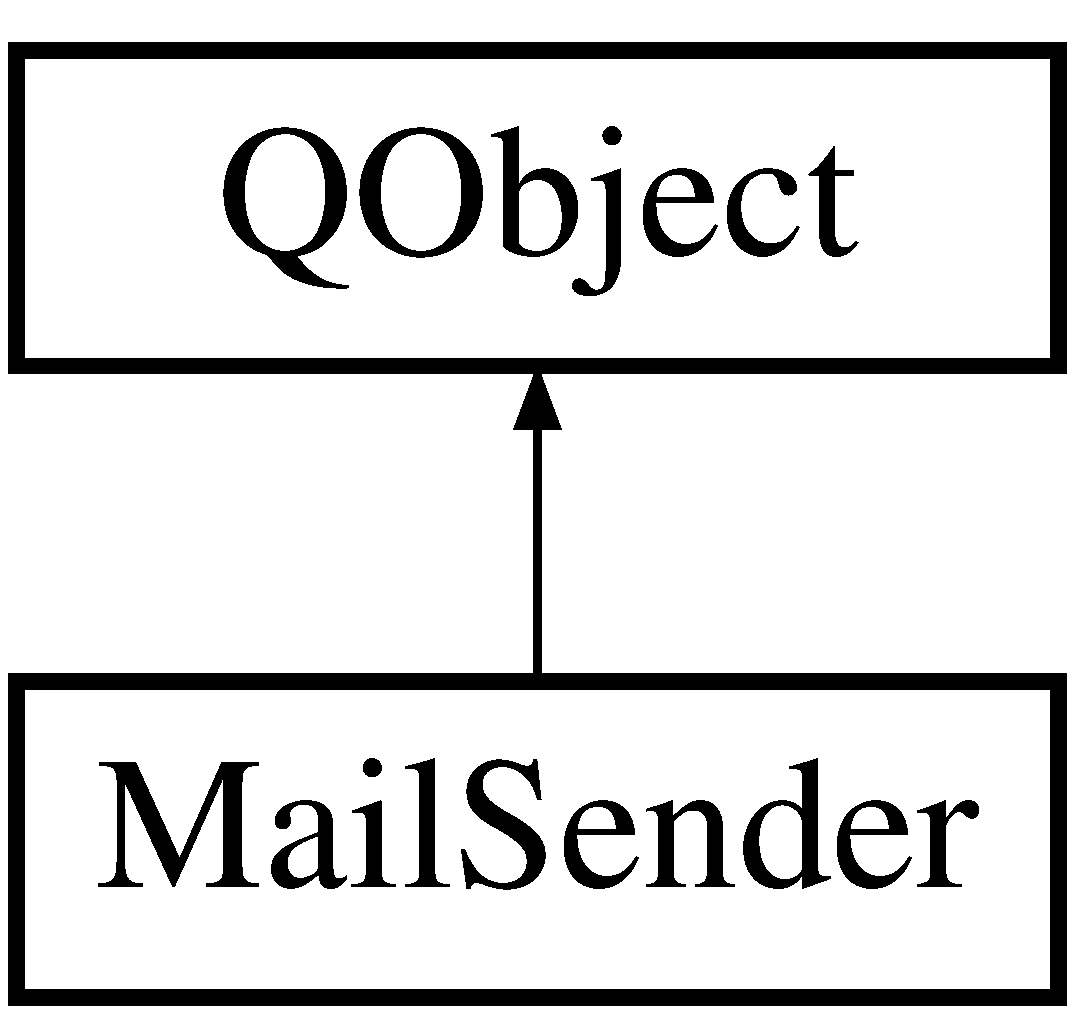
\includegraphics[height=2.000000cm]{classMailSender}
\end{center}
\end{figure}
\subsubsection*{Public Slots}
\begin{DoxyCompactItemize}
\item 
void \mbox{\hyperlink{classMailSender_ab2086805ee1168d42959ddbe7231bf5f}{set\+Recipient\+Mail\+Adress}} (Q\+String mail=\char`\"{}mishko.\+litvin@gmail.\+com\char`\"{})
\item 
void \mbox{\hyperlink{classMailSender_a9e5b40867b2bc78a71d4e91afabbefc6}{set\+Email\+Subject}} (Q\+String subject=\char`\"{}Li\+Qt Machine interface autosend message\char`\"{})
\item 
void \mbox{\hyperlink{classMailSender_aba231256948b0abb340452b8f902955d}{set\+Recipient\+Name}} (Q\+String name=\char`\"{}Customer\char`\"{})
\item 
void \mbox{\hyperlink{classMailSender_a3da1ed689ff76134c9ba5704ae724951}{set\+Sender\+Mail\+Adress}} (Q\+String mail=\char`\"{}Liqt.\+autosend@gmail.\+com\char`\"{})
\item 
void \mbox{\hyperlink{classMailSender_a3d97c584ca24948d320d31d10cc74089}{set\+Sender\+Password}} (Q\+String pswd=\char`\"{}D7\+C5cq\+Az\char`\"{})
\item 
void \mbox{\hyperlink{classMailSender_a23f9bd461f1f7583e7669430b4f01b59}{set\+Sender\+Name}} (Q\+String name=\char`\"{}Li\+Qt Interface\char`\"{})
\end{DoxyCompactItemize}
\subsubsection*{Public Member Functions}
\begin{DoxyCompactItemize}
\item 
\mbox{\hyperlink{classMailSender_afad3d5334eb2ce670dd351d6e4578170}{Mail\+Sender}} (Q\+Object $\ast$parent=0)
\item 
int \mbox{\hyperlink{classMailSender_a57749e1c2f79dfe8d3c0dbb0e984f9b9}{send\+Message}} (Q\+String message\+Str, Q\+String subject, bool clear=true)
\item 
int \mbox{\hyperlink{classMailSender_afcfdcae3a5ffb196d8357866a9d19020}{send\+Message}} (Q\+String \mbox{\hyperlink{classMailSender_aacde6999850036655c9a4a5e99a4bead}{message}}, bool clear=true)
\end{DoxyCompactItemize}
\subsubsection*{Private Attributes}
\begin{DoxyCompactItemize}
\item 
Smtp\+Client $\ast$ \mbox{\hyperlink{classMailSender_af89aab8c2f9788360352e89e3434988d}{smtp}}
\item 
Mime\+Message $\ast$ \mbox{\hyperlink{classMailSender_aacde6999850036655c9a4a5e99a4bead}{message}}
\item 
Email\+Address $\ast$ \mbox{\hyperlink{classMailSender_a07af5d8ff3491cc11187f28bfbac85d8}{sender\+Addr}}
\item 
Email\+Address $\ast$ \mbox{\hyperlink{classMailSender_a9979dc95139744a95d5814b2ea03174e}{recipient\+Addr}}
\item 
Mime\+Text $\ast$ \mbox{\hyperlink{classMailSender_a39b44ca80550570dfc8ae847038f271c}{message\+Text}}
\item 
Q\+String \mbox{\hyperlink{classMailSender_ab289a6d7038218f62211335320971427}{message\+Subject}}
\end{DoxyCompactItemize}


\subsubsection{Constructor \& Destructor Documentation}
\mbox{\Hypertarget{classMailSender_afad3d5334eb2ce670dd351d6e4578170}\label{classMailSender_afad3d5334eb2ce670dd351d6e4578170}} 
\index{Mail\+Sender@{Mail\+Sender}!Mail\+Sender@{Mail\+Sender}}
\index{Mail\+Sender@{Mail\+Sender}!Mail\+Sender@{Mail\+Sender}}
{\footnotesize\ttfamily Mail\+Sender\+::\texorpdfstring{Mail\+Sender()}{MailSender} (\begin{DoxyParamCaption}\item[{Q\+Object $\ast$}]{parent = {\ttfamily 0} }\end{DoxyParamCaption})\hspace{0.3cm}{\ttfamily [explicit]}} - standard class constructor. Initialize mail sender class with standard parameters.



\subsubsection{Member Function Documentation}
\mbox{\Hypertarget{classMailSender_a57749e1c2f79dfe8d3c0dbb0e984f9b9}\label{classMailSender_a57749e1c2f79dfe8d3c0dbb0e984f9b9}} 
\index{Mail\+Sender@{Mail\+Sender}!send\+Message@{send\+Message}}
\index{send\+Message@{send\+Message}!Mail\+Sender@{Mail\+Sender}}	
{\footnotesize\ttfamily int Mail\+Sender\+::\texorpdfstring{send\+Message}{sendMessage}\hspace{0.1cm}{\footnotesize\ttfamily [1/2]} (\begin{DoxyParamCaption}\item[{Q\+String}]{message\+Str,  }\item[{Q\+String}]{subject,  }\item[{bool}]{clear = {\ttfamily true} }\end{DoxyParamCaption})} - function to send message with \textit{message\+Str} and \textit{subject} by e-mail. 

\mbox{\Hypertarget{classMailSender_afcfdcae3a5ffb196d8357866a9d19020}\label{classMailSender_afcfdcae3a5ffb196d8357866a9d19020}} 
\index{Mail\+Sender@{Mail\+Sender}!send\+Message@{send\+Message}}
\index{send\+Message@{send\+Message}!Mail\+Sender@{Mail\+Sender}}
{\footnotesize\ttfamily int Mail\+Sender\+::\texorpdfstring{send\+Message}{sendMessage}\hspace{0.1cm}{\footnotesize\ttfamily [2/2]} (\begin{DoxyParamCaption}\item[{Q\+String}]{message,  }\item[{bool}]{clear = {\ttfamily true} }\end{DoxyParamCaption})} - function to send message with \textit{message\+Str} and  subject recorded by \mbox{\hyperlink{classMailSender_a9e5b40867b2bc78a71d4e91afabbefc6}{set\+Email\+Subject}}(...) function with e-mail. \\

\begin{center}	\line(1,0){450} \end{center}
Block of function which used for setup parameters of e-mail messages. 
\begin{DoxyCompactItemize}
\item\mbox{\Hypertarget{classMailSender_a9e5b40867b2bc78a71d4e91afabbefc6}\label{classMailSender_a9e5b40867b2bc78a71d4e91afabbefc6}} 
\index{Mail\+Sender@{Mail\+Sender}!set\+Email\+Subject@{set\+Email\+Subject}}
\index{set\+Email\+Subject@{set\+Email\+Subject}!Mail\+Sender@{Mail\+Sender}}
{\footnotesize\ttfamily void Mail\+Sender\+::\texorpdfstring{set\+Email\+Subject}{setEmailSubject} (\begin{DoxyParamCaption}\item[{Q\+String}]{subject = {\ttfamily \char`\"{}LiQt~Machine~interface~autosend~{message}\char`\"{}} }\end{DoxyParamCaption})\hspace{0.3cm}{\ttfamily [slot]}} 

\item\mbox{\Hypertarget{classMailSender_ab2086805ee1168d42959ddbe7231bf5f}\label{classMailSender_ab2086805ee1168d42959ddbe7231bf5f}} 
\index{Mail\+Sender@{Mail\+Sender}!set\+Recipient\+Mail\+Adress@{set\+Recipient\+Mail\+Adress}}
\index{set\+Recipient\+Mail\+Adress@{set\+Recipient\+Mail\+Adress}!Mail\+Sender@{Mail\+Sender}}
{\footnotesize\ttfamily void Mail\+Sender\+::\texorpdfstring{set\+Recipient\+Mail\+Adress}{setRecipientMailAdress} (\begin{DoxyParamCaption}\item[{Q\+String}]{mail = {\ttfamily \char`\"{}mishko.litvin@gmail.com\char`\"{}} }\end{DoxyParamCaption})\hspace{0.3cm}{\ttfamily [slot]}}

\item\mbox{\Hypertarget{classMailSender_aba231256948b0abb340452b8f902955d}\label{classMailSender_aba231256948b0abb340452b8f902955d}} 
\index{Mail\+Sender@{Mail\+Sender}!set\+Recipient\+Name@{set\+Recipient\+Name}}
\index{set\+Recipient\+Name@{set\+Recipient\+Name}!Mail\+Sender@{Mail\+Sender}}
{\footnotesize\ttfamily void Mail\+Sender\+::\texorpdfstring{set\+Recipient\+Name}{setRecipientName} (\begin{DoxyParamCaption}\item[{Q\+String}]{name = {\ttfamily \char`\"{}Customer\char`\"{}} }\end{DoxyParamCaption})\hspace{0.3cm}{\ttfamily [slot]}}

\item\mbox{\Hypertarget{classMailSender_a3da1ed689ff76134c9ba5704ae724951}\label{classMailSender_a3da1ed689ff76134c9ba5704ae724951}} 
\index{Mail\+Sender@{Mail\+Sender}!set\+Sender\+Mail\+Adress@{set\+Sender\+Mail\+Adress}}
\index{set\+Sender\+Mail\+Adress@{set\+Sender\+Mail\+Adress}!Mail\+Sender@{Mail\+Sender}}
{\footnotesize\ttfamily void Mail\+Sender\+::\texorpdfstring{set\+Sender\+Mail\+Adress}{setSenderMailAdress} (\begin{DoxyParamCaption}\item[{Q\+String}]{mail = {\ttfamily \char`\"{}Liqt.autosend@gmail.com\char`\"{}} }\end{DoxyParamCaption})\hspace{0.3cm}{\ttfamily [slot]}}

\item\mbox{\Hypertarget{classMailSender_a23f9bd461f1f7583e7669430b4f01b59}\label{classMailSender_a23f9bd461f1f7583e7669430b4f01b59}} 
\index{Mail\+Sender@{Mail\+Sender}!set\+Sender\+Name@{set\+Sender\+Name}}
\index{set\+Sender\+Name@{set\+Sender\+Name}!Mail\+Sender@{Mail\+Sender}}
{\footnotesize\ttfamily void Mail\+Sender\+::\texorpdfstring{set\+Sender\+Name}{setSenderName} (\begin{DoxyParamCaption}\item[{Q\+String}]{name = {\ttfamily \char`\"{}LiQt~Interface\char`\"{}} }\end{DoxyParamCaption})\hspace{0.3cm}{\ttfamily [slot]}}

\item\mbox{\Hypertarget{classMailSender_a3d97c584ca24948d320d31d10cc74089}\label{classMailSender_a3d97c584ca24948d320d31d10cc74089}} 
\index{Mail\+Sender@{Mail\+Sender}!set\+Sender\+Password@{set\+Sender\+Password}}
\index{set\+Sender\+Password@{set\+Sender\+Password}!Mail\+Sender@{Mail\+Sender}}
{\footnotesize\ttfamily void Mail\+Sender\+::\texorpdfstring{set\+Sender\+Password}{setSenderPassword} (\begin{DoxyParamCaption}\item[{Q\+String}]{pswd = {\ttfamily \char`\"{}D7C5cqAz\char`\"{}} }\end{DoxyParamCaption})\hspace{0.3cm}{\ttfamily [slot]}}
\end{DoxyCompactItemize}
\begin{center}	\line(1,0){450} \end{center}
\subsubsection{Member Data Documentation}
\mbox{\Hypertarget{classMailSender_aacde6999850036655c9a4a5e99a4bead}\label{classMailSender_aacde6999850036655c9a4a5e99a4bead}} 
\index{Mail\+Sender@{Mail\+Sender}!message@{message}}
\index{message@{message}!Mail\+Sender@{Mail\+Sender}}
{\footnotesize\ttfamily Mime\+Message$\ast$ Mail\+Sender\+::\texorpdfstring{message}{message}\hspace{0.3cm}{\ttfamily [private]}}

\mbox{\Hypertarget{classMailSender_ab289a6d7038218f62211335320971427}\label{classMailSender_ab289a6d7038218f62211335320971427}} 
\index{Mail\+Sender@{Mail\+Sender}!message\+Subject@{message\+Subject}}
\index{message\+Subject@{message\+Subject}!Mail\+Sender@{Mail\+Sender}}
{\footnotesize\ttfamily Q\+String Mail\+Sender\+::\texorpdfstring{message\+Subject}{messageSubject}\hspace{0.3cm}{\ttfamily [private]}}

\mbox{\Hypertarget{classMailSender_a39b44ca80550570dfc8ae847038f271c}\label{classMailSender_a39b44ca80550570dfc8ae847038f271c}} 
\index{Mail\+Sender@{Mail\+Sender}!message\+Text@{message\+Text}}
\index{message\+Text@{message\+Text}!Mail\+Sender@{Mail\+Sender}}
{\footnotesize\ttfamily Mime\+Text$\ast$ Mail\+Sender\+::\texorpdfstring{message\+Text}{messageText}\hspace{0.3cm}{\ttfamily [private]}}

\mbox{\Hypertarget{classMailSender_a9979dc95139744a95d5814b2ea03174e}\label{classMailSender_a9979dc95139744a95d5814b2ea03174e}} 
\index{Mail\+Sender@{Mail\+Sender}!recipient\+Addr@{recipient\+Addr}}
\index{recipient\+Addr@{recipient\+Addr}!Mail\+Sender@{Mail\+Sender}}
{\footnotesize\ttfamily Email\+Address$\ast$ Mail\+Sender\+::\texorpdfstring{recipient\+Addr}{recipientAddr}\hspace{0.3cm}{\ttfamily [private]}}

\mbox{\Hypertarget{classMailSender_a07af5d8ff3491cc11187f28bfbac85d8}\label{classMailSender_a07af5d8ff3491cc11187f28bfbac85d8}} 
\index{Mail\+Sender@{Mail\+Sender}!sender\+Addr@{sender\+Addr}}
\index{sender\+Addr@{sender\+Addr}!Mail\+Sender@{Mail\+Sender}}
{\footnotesize\ttfamily Email\+Address$\ast$ Mail\+Sender\+::\texorpdfstring{sender\+Addr}{senderAddr}\hspace{0.3cm}{\ttfamily [private]}}

\mbox{\Hypertarget{classMailSender_af89aab8c2f9788360352e89e3434988d}\label{classMailSender_af89aab8c2f9788360352e89e3434988d}} 
\index{Mail\+Sender@{Mail\+Sender}!smtp@{smtp}}
\index{smtp@{smtp}!Mail\+Sender@{Mail\+Sender}}
{\footnotesize\ttfamily Smtp\+Client$\ast$ Mail\+Sender\+::\texorpdfstring{smtp}{smtp}\hspace{0.3cm}{\ttfamily [private]}}



The documentation for this class was generated from the following files\+:\begin{DoxyCompactItemize}
\item 
\mbox{\hyperlink{mailsender_8h}{mailsender.\+h}}\item 
\mbox{\hyperlink{mailsender_8cpp}{mailsender.\+cpp}}\end{DoxyCompactItemize}
\newpage
\hypertarget{classMaintanceDialog}{}\subsection{Maintance\+Dialog Class Reference}
\label{classMaintanceDialog}\index{Maintance\+Dialog@{Maintance\+Dialog}}


{\ttfamily \#include $<$maintancedialog.\+h$>$}

Inheritance diagram for Maintance\+Dialog\+:\begin{figure}[H]
\begin{center}
\leavevmode
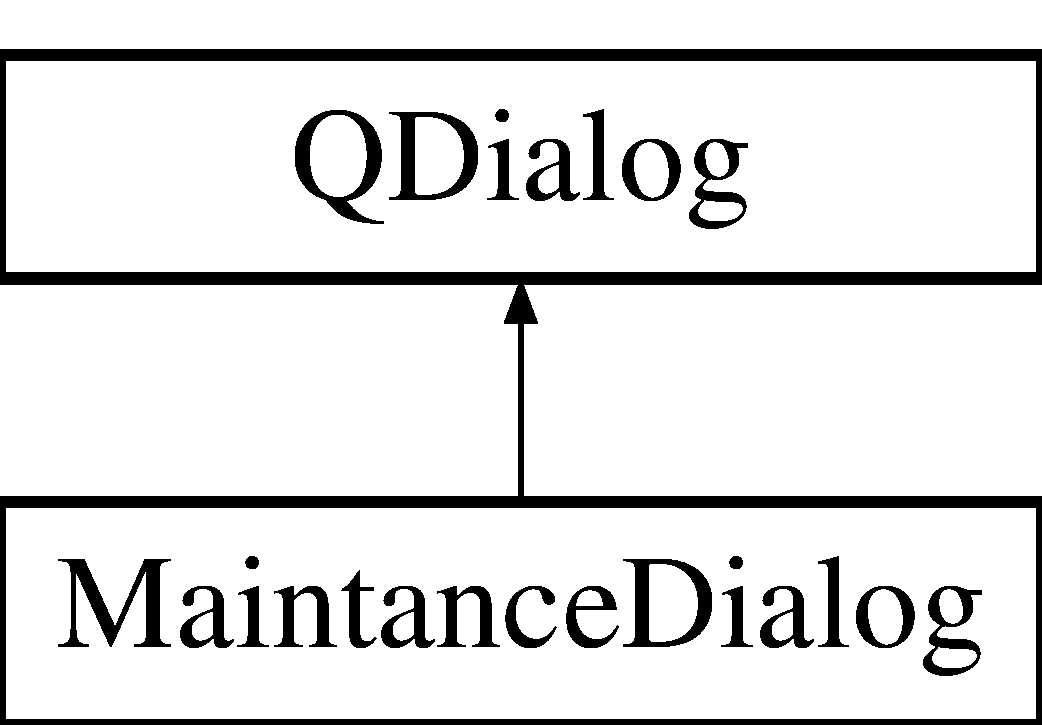
\includegraphics[height=2.000000cm]{classMaintanceDialog}
\end{center}
\end{figure}
\subsubsection*{Public Types}
\begin{DoxyCompactItemize}
\item 
enum \mbox{\hyperlink{classMaintanceDialog_a0774fde5cbe916c333d8d1dd991a3b8f}{Maintance\+Type}} \{ \mbox{\hyperlink{classMaintanceDialog_a0774fde5cbe916c333d8d1dd991a3b8fa8fe148a4b5ff71d3568fd6aff35d027e}{Warning}}, 
\mbox{\hyperlink{classMaintanceDialog_a0774fde5cbe916c333d8d1dd991a3b8fa56052452a2261539060f7f5433d35d61}{Critical}}
 \}
\end{DoxyCompactItemize}
\subsubsection*{Public Slots}
\begin{DoxyCompactItemize}
\item 
void \mbox{\hyperlink{classMaintanceDialog_ab97eb55c76459c27bc3ccf5c6a515b1e}{open\+Maintance\+List}} ()
\item 
void \mbox{\hyperlink{classMaintanceDialog_a9abf5dd5b908282f9f81f266708dd456}{open\+Dialog}} ()
\item 
void \mbox{\hyperlink{classMaintanceDialog_a3958b309d854fcd5baf39fc166a6b5f6}{solve\+Item}} (int index)
\end{DoxyCompactItemize}
\subsubsection*{Signals}
\begin{DoxyCompactItemize}
\item 
void \mbox{\hyperlink{classMaintanceDialog_ae2420d128d65322e62fc88044b20f848}{stop\+Request}} ()
\item 
void \mbox{\hyperlink{classMaintanceDialog_aea9ae7ab9094dfb556fb9ec134b12609}{continue\+Request}} ()
\item 
void \mbox{\hyperlink{classMaintanceDialog_ada9e582be087bce2dd96a2629f2a417f}{maintance\+Work\+Enable}} (bool enabled)
\end{DoxyCompactItemize}
\subsubsection*{Public Member Functions}
\begin{DoxyCompactItemize}
\item 
\mbox{\hyperlink{classMaintanceDialog_a3f541a92622740cce0a8f66e5de506fd}{Maintance\+Dialog}} (Q\+Widget $\ast$parent=0)
\item 
\mbox{\hyperlink{classMaintanceDialog_adce1e1f1bf5989b01784faf777b8a40e}{Maintance\+Dialog}} (\mbox{\hyperlink{classMaintanceDialog_a0774fde5cbe916c333d8d1dd991a3b8f}{Maintance\+Type}} m\+Type, Q\+Widget $\ast$parent=0, Q\+String name=\char`\"{}trouble\char`\"{}, Q\+String tr\+Info=\char`\"{}trouble info\char`\"{}, Q\+String mach\+Info=\char`\"{}machine info\char`\"{})
\item 
\mbox{\hyperlink{classMaintanceDialog_a96b4b3c7702a5a3fb51c7d5327cb82e1}{$\sim$\+Maintance\+Dialog}} ()
\item 
void \mbox{\hyperlink{classMaintanceDialog_a2f690d0f71452b2471282fdba269928b}{set\+Trable\+Name}} (Q\+String name=\char`\"{}trouble\char`\"{})
\item 
void \mbox{\hyperlink{classMaintanceDialog_a7f1a8997a72655a25eb57975c5535736}{set\+Trable\+Info}} (Q\+String info=\char`\"{}trouble info\char`\"{})
\item 
void \mbox{\hyperlink{classMaintanceDialog_a9c71badea52d72c56dee328a7de15005}{set\+Machine\+Info}} (Q\+String info=\char`\"{}machine info\char`\"{})
\item 
void \mbox{\hyperlink{classMaintanceDialog_a38b7cab71ff559010bef483adec52227}{set\+Maintance\+Type}} (\mbox{\hyperlink{classMaintanceDialog_a0774fde5cbe916c333d8d1dd991a3b8f}{Maintance\+Type}} m\+Type=\mbox{\hyperlink{classMaintanceDialog_a0774fde5cbe916c333d8d1dd991a3b8fa8fe148a4b5ff71d3568fd6aff35d027e}{Warning}})
\item 
Q\+List$<$ \mbox{\hyperlink{classMaintanceElement}{Maintance\+Element}} $>$ \mbox{\hyperlink{classMaintanceDialog_af304179c775853116b308ed635f8d027}{get\+Unsolved\+List}} ()
\item 
void \mbox{\hyperlink{classMaintanceDialog_a0eb162bfea71b4712de3cc63cc6bb0f5}{check}} (int cycles\+Count)
\end{DoxyCompactItemize}
\subsubsection*{Static Public Member Functions}
\begin{DoxyCompactItemize}
\item 
static bool \mbox{\hyperlink{classMaintanceDialog_adf3b798d56bad8af60553f9e04fad8a4}{execute}} (Q\+Widget $\ast$parent=0, \mbox{\hyperlink{classMaintanceDialog_a0774fde5cbe916c333d8d1dd991a3b8f}{Maintance\+Type}} m\+Type=\mbox{\hyperlink{classMaintanceDialog_a0774fde5cbe916c333d8d1dd991a3b8fa8fe148a4b5ff71d3568fd6aff35d027e}{Warning}}, Q\+String name=\char`\"{}trouble\char`\"{}, Q\+String tr\+Info=\char`\"{}trouble info\char`\"{}, Q\+String mach\+Info=\char`\"{}machine info\char`\"{})
\item 
static bool \mbox{\hyperlink{classMaintanceDialog_a1c21277543efab3d8207b64de9d8ba20}{execute}} (\mbox{\hyperlink{classMaintanceElement}{Maintance\+Element}} maintance, Q\+Widget $\ast$parent=0)
\end{DoxyCompactItemize}
\subsubsection*{Protected Member Functions}
\begin{DoxyCompactItemize}
\item 
void \mbox{\hyperlink{classMaintanceDialog_a2bd5d68e291648614735e3b62fd61bfc}{change\+Event}} (Q\+Event $\ast$event)
\end{DoxyCompactItemize}
\subsubsection*{Private Slots}
\begin{DoxyCompactItemize}
\item 
void \mbox{\hyperlink{classMaintanceDialog_a3453a9ed317177d9bf8fb4be6bfa9de6}{accept\+Slot}} ()
\item 
void \mbox{\hyperlink{classMaintanceDialog_aa92ce781e64b49dab9cb362c6521bb17}{reject\+Slot}} ()
\end{DoxyCompactItemize}
\subsubsection*{Private Attributes}
\begin{DoxyCompactItemize}
\item 
Ui\+::\+Maintance\+Dialog $\ast$ \mbox{\hyperlink{classMaintanceDialog_aee97dd9f83af9508fb0ed3ac2de6ba87}{ui}}
\item 
bool \mbox{\hyperlink{classMaintanceDialog_ae23009895f32bfffb43f5ed93188be45}{do\+It\+Now}}
\item 
bool \mbox{\hyperlink{classMaintanceDialog_aea111f8bf60829f66b3f93c842512dea}{maintance\+Have\+Work}}
\item 
bool \mbox{\hyperlink{classMaintanceDialog_afe855bd63066dc98f09758b7cd6d9b53}{maintance\+Have\+Warning}}
\item 
Q\+Settings $\ast$ \mbox{\hyperlink{classMaintanceDialog_ad41c158948e59029193b28d4e3ab309e}{settings}}
\item 
Q\+List$<$ \mbox{\hyperlink{classMaintanceElement}{Maintance\+Element}} $>$ \mbox{\hyperlink{classMaintanceDialog_ac4eade50e2d9071c65adf44a2987fab1}{maintance\+List}}
\item 
Q\+List$<$ \mbox{\hyperlink{classMaintanceElement}{Maintance\+Element}} $>$ \mbox{\hyperlink{classMaintanceDialog_a37e3caf05435d01f47ed488c39a91587}{unsolved\+List}}
\item 
Q\+List$<$ int $>$ \mbox{\hyperlink{classMaintanceDialog_aae5f5335ab6b848ea0ff6254abbcece3}{unsolved\+List\+Index}}
\item 
\mbox{\hyperlink{classMaintanceWidget}{Maintance\+Widget}} $\ast$ \mbox{\hyperlink{classMaintanceDialog_a42a95d76614ce637c9b332ff996020e2}{maintance\+Widget}}
\item 
bool \mbox{\hyperlink{classMaintanceDialog_a27e8f4e6881da67cec3568a4a4b757a1}{first\+Check}}
\item 
int \mbox{\hyperlink{classMaintanceDialog_a615b6ffbbda8324d5225d286570f7f31}{last\+Cycles\+Count}}
\end{DoxyCompactItemize}


\subsubsection{Member Enumeration Documentation}
\mbox{\Hypertarget{classMaintanceDialog_a0774fde5cbe916c333d8d1dd991a3b8f}\label{classMaintanceDialog_a0774fde5cbe916c333d8d1dd991a3b8f}} 
\index{Maintance\+Dialog@{Maintance\+Dialog}!Maintance\+Type@{Maintance\+Type}}
\index{Maintance\+Type@{Maintance\+Type}!Maintance\+Dialog@{Maintance\+Dialog}}
\paragraph{\texorpdfstring{Maintance\+Type}{MaintanceType}}
{\footnotesize\ttfamily enum \mbox{\hyperlink{classMaintanceDialog_a0774fde5cbe916c333d8d1dd991a3b8f}{Maintance\+Dialog\+::\+Maintance\+Type}}}

\begin{DoxyEnumFields}{Enumerator}
\raisebox{\heightof{T}}[0pt][0pt]{\index{Warning@{Warning}!Maintance\+Dialog@{Maintance\+Dialog}}\index{Maintance\+Dialog@{Maintance\+Dialog}!Warning@{Warning}}}\mbox{\Hypertarget{classMaintanceDialog_a0774fde5cbe916c333d8d1dd991a3b8fa8fe148a4b5ff71d3568fd6aff35d027e}\label{classMaintanceDialog_a0774fde5cbe916c333d8d1dd991a3b8fa8fe148a4b5ff71d3568fd6aff35d027e}} 
Warning&\\
\hline

\raisebox{\heightof{T}}[0pt][0pt]{\index{Critical@{Critical}!Maintance\+Dialog@{Maintance\+Dialog}}\index{Maintance\+Dialog@{Maintance\+Dialog}!Critical@{Critical}}}\mbox{\Hypertarget{classMaintanceDialog_a0774fde5cbe916c333d8d1dd991a3b8fa56052452a2261539060f7f5433d35d61}\label{classMaintanceDialog_a0774fde5cbe916c333d8d1dd991a3b8fa56052452a2261539060f7f5433d35d61}} 
Critical&\\
\hline

\end{DoxyEnumFields}


\subsubsection{Constructor \& Destructor Documentation}
\mbox{\Hypertarget{classMaintanceDialog_a3f541a92622740cce0a8f66e5de506fd}\label{classMaintanceDialog_a3f541a92622740cce0a8f66e5de506fd}} 
\index{Maintance\+Dialog@{Maintance\+Dialog}!Maintance\+Dialog@{Maintance\+Dialog}}
\index{Maintance\+Dialog@{Maintance\+Dialog}!Maintance\+Dialog@{Maintance\+Dialog}}
{\footnotesize\ttfamily \texorpdfstring{Maintance\+Dialog()}{MaintanceDialog()}\hspace{0.1cm}{\footnotesize\ttfamily [1/2]} (\begin{DoxyParamCaption}\item[{Q\+Widget $\ast$}]{parent = {\ttfamily 0} }\end{DoxyParamCaption})\hspace{0.3cm}{\ttfamily [explicit]}} - standard Q\+Dialog class constructor. Lists \hyperlink{classMaintanceDialog_ac4eade50e2d9071c65adf44a2987fab1}{maintance\+List},  \hyperlink{classMaintanceDialog_a37e3caf05435d01f47ed488c39a91587}{unsolved\+List} and \hyperlink{classMaintanceDialog_aae5f5335ab6b848ea0ff6254abbcece3}{unsolved\+List\+Index} are fill in constructor. 

\mbox{\Hypertarget{classMaintanceDialog_adce1e1f1bf5989b01784faf777b8a40e}\label{classMaintanceDialog_adce1e1f1bf5989b01784faf777b8a40e}} 
\index{Maintance\+Dialog@{Maintance\+Dialog}!Maintance\+Dialog@{Maintance\+Dialog}}
\index{Maintance\+Dialog@{Maintance\+Dialog}!Maintance\+Dialog@{Maintance\+Dialog}}
{\footnotesize\ttfamily \texorpdfstring{Maintance\+Dialog()}{MaintanceDialog()}\hspace{0.1cm}{\footnotesize\ttfamily [2/2]} (\begin{DoxyParamCaption}\item[{\mbox{\hyperlink{classMaintanceDialog_a0774fde5cbe916c333d8d1dd991a3b8f}{Maintance\+Dialog\+::\+Maintance\+Type}}}]{m\+Type,  }\item[{Q\+Widget $\ast$}]{parent = {\ttfamily 0},  }\item[{Q\+String}]{name = {\ttfamily \char`\"{}trouble\char`\"{}},  }\item[{Q\+String}]{tr\+Info = {\ttfamily \char`\"{}trouble~info\char`\"{}},  }\item[{Q\+String}]{mach\+Info = {\ttfamily \char`\"{}machine~info\char`\"{}} }\end{DoxyParamCaption})\hspace{0.3cm}{\ttfamily [explicit]}} - reimplemented constructor of class. Used to fill appropriated fields on user interface. 

\mbox{\Hypertarget{classMaintanceDialog_a96b4b3c7702a5a3fb51c7d5327cb82e1}\label{classMaintanceDialog_a96b4b3c7702a5a3fb51c7d5327cb82e1}} 
\index{Maintance\+Dialog@{Maintance\+Dialog}!````~Maintance\+Dialog@{$\sim$\+Maintance\+Dialog}}
\index{````~Maintance\+Dialog@{$\sim$\+Maintance\+Dialog}!Maintance\+Dialog@{Maintance\+Dialog}}
{\footnotesize\ttfamily \texorpdfstring{$\sim$\+Maintance\+Dialog()}{~MaintanceDialog()} 
(\begin{DoxyParamCaption}{ }\end{DoxyParamCaption})} - standard Q\+Dialog class destructor.



\subsubsection{Member Function Documentation}
\mbox{\Hypertarget{classMaintanceDialog_a3453a9ed317177d9bf8fb4be6bfa9de6}\label{classMaintanceDialog_a3453a9ed317177d9bf8fb4be6bfa9de6}} 
\index{Maintance\+Dialog@{Maintance\+Dialog}!accept\+Slot@{accept\+Slot}}
\index{accept\+Slot@{accept\+Slot}!Maintance\+Dialog@{Maintance\+Dialog}}
{\footnotesize\ttfamily void Maintance\+Dialog\+::\texorpdfstring{accept\+Slot}{acceptSlot} (\begin{DoxyParamCaption}{ }\end{DoxyParamCaption})\hspace{0.3cm}{\ttfamily [private]}, {\ttfamily [slot]}} - function used to set \textit{true} to \hyperlink{classMaintanceDialog_ae23009895f32bfffb43f5ed93188be45}{do\+It\+Now} variable and exit from dialog;

\mbox{\Hypertarget{classMaintanceDialog_a2bd5d68e291648614735e3b62fd61bfc}\label{classMaintanceDialog_a2bd5d68e291648614735e3b62fd61bfc}} 
\index{Maintance\+Dialog@{Maintance\+Dialog}!change\+Event@{change\+Event}}
\index{change\+Event@{change\+Event}!Maintance\+Dialog@{Maintance\+Dialog}}
{\footnotesize\ttfamily void Maintance\+Dialog\+::\texorpdfstring{change\+Event}{changeEvent} (\begin{DoxyParamCaption}\item[{Q\+Event $\ast$}]{event }\end{DoxyParamCaption})\hspace{0.3cm}{\ttfamily [protected]}}- reimplementation of default event for Q\+Dialog to enable user interface translation. Function called automatically.

\mbox{\Hypertarget{classMaintanceDialog_a0eb162bfea71b4712de3cc63cc6bb0f5}\label{classMaintanceDialog_a0eb162bfea71b4712de3cc63cc6bb0f5}} 
\index{Maintance\+Dialog@{Maintance\+Dialog}!check@{check}}
\index{check@{check}!Maintance\+Dialog@{Maintance\+Dialog}}
{\footnotesize\ttfamily void Maintance\+Dialog\+::\texorpdfstring{check}{check} (\begin{DoxyParamCaption}\item[{int}]{cycles\+Count }\end{DoxyParamCaption})} - function used to check does machine must stop for maintenance. Function called at every indexer step and check all maintenance items (from \hyperlink{classMaintanceDialog_ac4eade50e2d9071c65adf44a2987fab1}{maintance\+List}). Function emits \hyperlink{classMaintanceDialog_ada9e582be087bce2dd96a2629f2a417f}{maintance\+Work\+Enable}(...) signal with appropriate value.

\mbox{\Hypertarget{classMaintanceDialog_aea9ae7ab9094dfb556fb9ec134b12609}\label{classMaintanceDialog_aea9ae7ab9094dfb556fb9ec134b12609}} 
\index{Maintance\+Dialog@{Maintance\+Dialog}!continue\+Request@{continue\+Request}}
\index{continue\+Request@{continue\+Request}!Maintance\+Dialog@{Maintance\+Dialog}}
{\footnotesize\ttfamily void Maintance\+Dialog\+::\texorpdfstring{continue\+Request}{continueRequest} (\begin{DoxyParamCaption}{ }\end{DoxyParamCaption})\hspace{0.3cm}{\ttfamily [signal]}} - unused.

\mbox{\Hypertarget{classMaintanceDialog_adf3b798d56bad8af60553f9e04fad8a4}\label{classMaintanceDialog_adf3b798d56bad8af60553f9e04fad8a4}} 
\index{Maintance\+Dialog@{Maintance\+Dialog}!execute@{execute}}
\index{execute@{execute}!Maintance\+Dialog@{Maintance\+Dialog}}
{\footnotesize\ttfamily bool Maintance\+Dialog\+::\texorpdfstring{execute}{execute}\hspace{0.1cm}{\footnotesize\ttfamily [1/2]} (\begin{DoxyParamCaption}\item[{Q\+Widget $\ast$}]{parent = {\ttfamily 0},  }\item[{\mbox{\hyperlink{classMaintanceDialog_a0774fde5cbe916c333d8d1dd991a3b8f}{Maintance\+Dialog\+::\+Maintance\+Type}}}]{m\+Type = {\ttfamily \mbox{\hyperlink{classMaintanceDialog_a0774fde5cbe916c333d8d1dd991a3b8fa8fe148a4b5ff71d3568fd6aff35d027e}{Warning}}},  }\item[{Q\+String}]{name = {\ttfamily \char`\"{}trouble\char`\"{}},  }\item[{Q\+String}]{tr\+Info = {\ttfamily \char`\"{}trouble~info\char`\"{}},  }\item[{Q\+String}]{mach\+Info = {\ttfamily \char`\"{}machine~info\char`\"{}} }\end{DoxyParamCaption})\hspace{0.3cm}{\ttfamily [static]}} - function used to call \hyperlink{classMaintanceDialog_adce1e1f1bf5989b01784faf777b8a40e}{Maintance\+Dialog}(...) constructor with appropriate parameters given in function.

\mbox{\Hypertarget{classMaintanceDialog_a1c21277543efab3d8207b64de9d8ba20}\label{classMaintanceDialog_a1c21277543efab3d8207b64de9d8ba20}} 
\index{Maintance\+Dialog@{Maintance\+Dialog}!execute@{execute}}
\index{execute@{execute}!Maintance\+Dialog@{Maintance\+Dialog}}
{\footnotesize\ttfamily bool Maintance\+Dialog\+::\texorpdfstring{execute}{execute}\hspace{0.1cm}{\footnotesize\ttfamily [2/2]} (\begin{DoxyParamCaption}\item[{\mbox{\hyperlink{classMaintanceElement}{Maintance\+Element}}}]{maintance,  }\item[{Q\+Widget $\ast$}]{parent = {\ttfamily 0} }\end{DoxyParamCaption})\hspace{0.3cm}{\ttfamily [static]}} - function used to call \hyperlink{classMaintanceDialog_adce1e1f1bf5989b01784faf777b8a40e}{Maintance\+Dialog}(...) constructor with parameters taken from \textit{maintance} variable.

\mbox{\Hypertarget{classMaintanceDialog_af304179c775853116b308ed635f8d027}\label{classMaintanceDialog_af304179c775853116b308ed635f8d027}} 
\index{Maintance\+Dialog@{Maintance\+Dialog}!get\+Unsolved\+List@{get\+Unsolved\+List}}
\index{get\+Unsolved\+List@{get\+Unsolved\+List}!Maintance\+Dialog@{Maintance\+Dialog}}
{\footnotesize\ttfamily Q\+List$<$ \mbox{\hyperlink{classMaintanceElement}{Maintance\+Element}} $>$ Maintance\+Dialog\+::\texorpdfstring{get\+Unsolved\+List}{getUnsolvedList} (\begin{DoxyParamCaption}{ }\end{DoxyParamCaption})} - function used to get \hyperlink{classMaintanceDialog_a37e3caf05435d01f47ed488c39a91587}{unsolved\+List} variable value.

\mbox{\Hypertarget{classMaintanceDialog_ada9e582be087bce2dd96a2629f2a417f}\label{classMaintanceDialog_ada9e582be087bce2dd96a2629f2a417f}} 
\index{Maintance\+Dialog@{Maintance\+Dialog}!maintance\+Work\+Enable@{maintance\+Work\+Enable}}
\index{maintance\+Work\+Enable@{maintance\+Work\+Enable}!Maintance\+Dialog@{Maintance\+Dialog}}
{\footnotesize\ttfamily void Maintance\+Dialog\+::\texorpdfstring{maintance\+Work\+Enable}{maintanceWorkEnable} (\begin{DoxyParamCaption}\item[{bool}]{enabled }\end{DoxyParamCaption})\hspace{0.3cm}{\ttfamily [signal]}} - signal which emitted by \hyperlink{classMaintanceDialog_a0eb162bfea71b4712de3cc63cc6bb0f5}{check}(...) function and handle in parent object. Value which send with signal sets in function.

\mbox{\Hypertarget{classMaintanceDialog_a9abf5dd5b908282f9f81f266708dd456}\label{classMaintanceDialog_a9abf5dd5b908282f9f81f266708dd456}} 
\index{Maintance\+Dialog@{Maintance\+Dialog}!open\+Dialog@{open\+Dialog}}
\index{open\+Dialog@{open\+Dialog}!Maintance\+Dialog@{Maintance\+Dialog}}
{\footnotesize\ttfamily void Maintance\+Dialog\+::\texorpdfstring{open\+Dialog}{openDialog} (\begin{DoxyParamCaption}{ }\end{DoxyParamCaption})\hspace{0.3cm}{\ttfamily [slot]}} - function used to open dialogs fo every item in \hyperlink{classMaintanceDialog_a37e3caf05435d01f47ed488c39a91587}{unsolved\+List}.

\mbox{\Hypertarget{classMaintanceDialog_ab97eb55c76459c27bc3ccf5c6a515b1e}\label{classMaintanceDialog_ab97eb55c76459c27bc3ccf5c6a515b1e}} 
\index{Maintance\+Dialog@{Maintance\+Dialog}!open\+Maintance\+List@{open\+Maintance\+List}}
\index{open\+Maintance\+List@{open\+Maintance\+List}!Maintance\+Dialog@{Maintance\+Dialog}}
{\footnotesize\ttfamily void Maintance\+Dialog\+::\texorpdfstring{open\+Maintance\+List}{openMaintanceList} (\begin{DoxyParamCaption}{ }\end{DoxyParamCaption})\hspace{0.3cm}{\ttfamily [slot]}}

\mbox{\Hypertarget{classMaintanceDialog_aa92ce781e64b49dab9cb362c6521bb17}\label{classMaintanceDialog_aa92ce781e64b49dab9cb362c6521bb17}} 
\index{Maintance\+Dialog@{Maintance\+Dialog}!reject\+Slot@{reject\+Slot}}
\index{reject\+Slot@{reject\+Slot}!Maintance\+Dialog@{Maintance\+Dialog}}
{\footnotesize\ttfamily void Maintance\+Dialog\+::\texorpdfstring{reject\+Slot}{rejectSlot} (\begin{DoxyParamCaption}{ }\end{DoxyParamCaption})\hspace{0.3cm}{\ttfamily [private]}, {\ttfamily [slot]}} - function used to set \textit{false} to \hyperlink{classMaintanceDialog_ae23009895f32bfffb43f5ed93188be45}{do\+It\+Now} variable and exit from dialog;

\begin{center}	\line(1,0){450} \end{center}
Block of function which used for setup parameters and fill appropriate fields of user interface. 
\begin{DoxyCompactItemize}
\item\mbox{\Hypertarget{classMaintanceDialog_a9c71badea52d72c56dee328a7de15005}\label{classMaintanceDialog_a9c71badea52d72c56dee328a7de15005}} 
\index{Maintance\+Dialog@{Maintance\+Dialog}!set\+Machine\+Info@{set\+Machine\+Info}}
\index{set\+Machine\+Info@{set\+Machine\+Info}!Maintance\+Dialog@{Maintance\+Dialog}}
{\footnotesize\ttfamily void Maintance\+Dialog\+::\texorpdfstring{set\+Machine\+Info()}{setMachineInfo()} (\begin{DoxyParamCaption}\item[{Q\+String}]{info = {\ttfamily \char`\"{}machine~info\char`\"{}} }\end{DoxyParamCaption})} 

\item\mbox{\Hypertarget{classMaintanceDialog_a38b7cab71ff559010bef483adec52227}\label{classMaintanceDialog_a38b7cab71ff559010bef483adec52227}} 
\index{Maintance\+Dialog@{Maintance\+Dialog}!set\+Maintance\+Type@{set\+Maintance\+Type}}
\index{set\+Maintance\+Type@{set\+Maintance\+Type}!Maintance\+Dialog@{Maintance\+Dialog}}
{\footnotesize\ttfamily void Maintance\+Dialog\+::\texorpdfstring{set\+Maintance\+Type()}{setMaintanceType()} (\begin{DoxyParamCaption}\item[{\mbox{\hyperlink{classMaintanceDialog_a0774fde5cbe916c333d8d1dd991a3b8f}{Maintance\+Dialog\+::\+Maintance\+Type}}}]{m\+Type = {\ttfamily \mbox{\hyperlink{classMaintanceDialog_a0774fde5cbe916c333d8d1dd991a3b8fa8fe148a4b5ff71d3568fd6aff35d027e}{Warning}}} }\end{DoxyParamCaption})}

\item\mbox{\Hypertarget{classMaintanceDialog_a7f1a8997a72655a25eb57975c5535736}\label{classMaintanceDialog_a7f1a8997a72655a25eb57975c5535736}} 
\index{Maintance\+Dialog@{Maintance\+Dialog}!set\+Trable\+Info@{set\+Trable\+Info}}
\index{set\+Trable\+Info@{set\+Trable\+Info}!Maintance\+Dialog@{Maintance\+Dialog}}
{\footnotesize\ttfamily void Maintance\+Dialog\+::\texorpdfstring{set\+Trable\+Info}{setTrableInfo} (\begin{DoxyParamCaption}\item[{Q\+String}]{info = {\ttfamily \char`\"{}trouble~info\char`\"{}} }\end{DoxyParamCaption})}

\item\mbox{\Hypertarget{classMaintanceDialog_a2f690d0f71452b2471282fdba269928b}\label{classMaintanceDialog_a2f690d0f71452b2471282fdba269928b}} 
\index{Maintance\+Dialog@{Maintance\+Dialog}!set\+Trable\+Name@{set\+Trable\+Name}}
\index{set\+Trable\+Name@{set\+Trable\+Name}!Maintance\+Dialog@{Maintance\+Dialog}}
{\footnotesize\ttfamily void Maintance\+Dialog\+::\texorpdfstring{set\+Trable\+Name}{setTrableName} (\begin{DoxyParamCaption}\item[{Q\+String}]{name = {\ttfamily \char`\"{}trouble\char`\"{}} }\end{DoxyParamCaption})}
\end{DoxyCompactItemize}
\begin{center}	\line(1,0){450} \end{center}

\mbox{\Hypertarget{classMaintanceDialog_a3958b309d854fcd5baf39fc166a6b5f6}\label{classMaintanceDialog_a3958b309d854fcd5baf39fc166a6b5f6}} 
\index{Maintance\+Dialog@{Maintance\+Dialog}!solve\+Item@{solve\+Item}}
\index{solve\+Item@{solve\+Item}!Maintance\+Dialog@{Maintance\+Dialog}}
{\footnotesize\ttfamily void Maintance\+Dialog\+::\texorpdfstring{solve\+Item}{solveItem} (\begin{DoxyParamCaption}\item[{int}]{index }\end{DoxyParamCaption})\hspace{0.3cm}{\ttfamily [slot]}} - function used to remove one item (number \textit{index}) from \hyperlink{classMaintanceDialog_a37e3caf05435d01f47ed488c39a91587}{unsolved\+List} and save \hyperlink{classMaintanceDialog_a37e3caf05435d01f47ed488c39a91587}{unsolved\+List} and \hyperlink{classMaintanceDialog_aae5f5335ab6b848ea0ff6254abbcece3}{unsolved\+List\+Index} to settings. If \hyperlink{classMaintanceDialog_aae5f5335ab6b848ea0ff6254abbcece3}{unsolved\+List\+Index} length is zero emits \hyperlink{classMaintanceDialog_ada9e582be087bce2dd96a2629f2a417f}{maintance\+Work\+Enable} (...) signal with \textit{false} value.

\mbox{\Hypertarget{classMaintanceDialog_ae2420d128d65322e62fc88044b20f848}\label{classMaintanceDialog_ae2420d128d65322e62fc88044b20f848}} 
\index{Maintance\+Dialog@{Maintance\+Dialog}!stop\+Request@{stop\+Request}}
\index{stop\+Request@{stop\+Request}!Maintance\+Dialog@{Maintance\+Dialog}}
{\footnotesize\ttfamily void Maintance\+Dialog\+::\texorpdfstring{stop\+Request}{stopRequest} (\begin{DoxyParamCaption}{ }\end{DoxyParamCaption})\hspace{0.3cm}{\ttfamily [signal]}} - unused.



\subsubsection{Member Data Documentation}
\mbox{\Hypertarget{classMaintanceDialog_ae23009895f32bfffb43f5ed93188be45}\label{classMaintanceDialog_ae23009895f32bfffb43f5ed93188be45}} 
\index{Maintance\+Dialog@{Maintance\+Dialog}!do\+It\+Now@{do\+It\+Now}}
\index{do\+It\+Now@{do\+It\+Now}!Maintance\+Dialog@{Maintance\+Dialog}}
{\footnotesize\ttfamily bool Maintance\+Dialog\+::\texorpdfstring{do\+It\+Now}{doItNow}\hspace{0.3cm}{\ttfamily [private]}}

\mbox{\Hypertarget{classMaintanceDialog_a27e8f4e6881da67cec3568a4a4b757a1}\label{classMaintanceDialog_a27e8f4e6881da67cec3568a4a4b757a1}} 
\index{Maintance\+Dialog@{Maintance\+Dialog}!first\+Check@{first\+Check}}
\index{first\+Check@{first\+Check}!Maintance\+Dialog@{Maintance\+Dialog}}
{\footnotesize\ttfamily bool Maintance\+Dialog\+::\texorpdfstring{first\+Check}{firstCheck}\hspace{0.3cm}{\ttfamily [private]}}

\mbox{\Hypertarget{classMaintanceDialog_a615b6ffbbda8324d5225d286570f7f31}\label{classMaintanceDialog_a615b6ffbbda8324d5225d286570f7f31}} 
\index{Maintance\+Dialog@{Maintance\+Dialog}!last\+Cycles\+Count@{last\+Cycles\+Count}}
\index{last\+Cycles\+Count@{last\+Cycles\+Count}!Maintance\+Dialog@{Maintance\+Dialog}}
{\footnotesize\ttfamily int Maintance\+Dialog\+:\texorpdfstring{last\+Cycles\+Count}{lastCyclesCount}\hspace{0.3cm}{\ttfamily [private]}}

\mbox{\Hypertarget{classMaintanceDialog_afe855bd63066dc98f09758b7cd6d9b53}\label{classMaintanceDialog_afe855bd63066dc98f09758b7cd6d9b53}} 
\index{Maintance\+Dialog@{Maintance\+Dialog}!maintance\+Have\+Warning@{maintance\+Have\+Warning}}
\index{maintance\+Have\+Warning@{maintance\+Have\+Warning}!Maintance\+Dialog@{Maintance\+Dialog}}
{\footnotesize\ttfamily bool Maintance\+Dialog\+::\texorpdfstring{maintance\+Have\+Warning}{maintanceHaveWarning}\hspace{0.3cm}{\ttfamily [private]}}

\mbox{\Hypertarget{classMaintanceDialog_aea111f8bf60829f66b3f93c842512dea}\label{classMaintanceDialog_aea111f8bf60829f66b3f93c842512dea}} 
\index{Maintance\+Dialog@{Maintance\+Dialog}!maintance\+Have\+Work@{maintance\+Have\+Work}}
\index{maintance\+Have\+Work@{maintance\+Have\+Work}!Maintance\+Dialog@{Maintance\+Dialog}}
{\footnotesize\ttfamily bool Maintance\+Dialog\+::\texorpdfstring{maintance\+Have\+Work}{maintanceHaveWork}\hspace{0.3cm}{\ttfamily [private]}}

\mbox{\Hypertarget{classMaintanceDialog_ac4eade50e2d9071c65adf44a2987fab1}\label{classMaintanceDialog_ac4eade50e2d9071c65adf44a2987fab1}} 
\index{Maintance\+Dialog@{Maintance\+Dialog}!maintance\+List@{maintance\+List}}
\index{maintance\+List@{maintance\+List}!Maintance\+Dialog@{Maintance\+Dialog}}
{\footnotesize\ttfamily Q\+List$<$\mbox{\hyperlink{classMaintanceElement}{Maintance\+Element}}$>$ Maintance\+Dialog\+::\texorpdfstring{maintance\+List}{maintanceList}\hspace{0.3cm}{\ttfamily [private]}}

\mbox{\Hypertarget{classMaintanceDialog_a42a95d76614ce637c9b332ff996020e2}\label{classMaintanceDialog_a42a95d76614ce637c9b332ff996020e2}} 
\index{Maintance\+Dialog@{Maintance\+Dialog}!maintance\+Widget@{maintance\+Widget}}
\index{maintance\+Widget@{maintance\+Widget}!Maintance\+Dialog@{Maintance\+Dialog}}
{\footnotesize\ttfamily \mbox{\hyperlink{classMaintanceWidget}{Maintance\+Widget}}$\ast$ Maintance\+Dialog\+::\texorpdfstring{maintance\+Widget}{maintanceWidget}\hspace{0.3cm}{\ttfamily [private]}}

\mbox{\Hypertarget{classMaintanceDialog_ad41c158948e59029193b28d4e3ab309e}\label{classMaintanceDialog_ad41c158948e59029193b28d4e3ab309e}} 
\index{Maintance\+Dialog@{Maintance\+Dialog}!settings@{settings}}
\index{settings@{settings}!Maintance\+Dialog@{Maintance\+Dialog}}
{\footnotesize\ttfamily Q\+Settings$\ast$ Maintance\+Dialog\+::\texorpdfstring{settings}{settings}\hspace{0.3cm}{\ttfamily [private]}}

\mbox{\Hypertarget{classMaintanceDialog_a37e3caf05435d01f47ed488c39a91587}\label{classMaintanceDialog_a37e3caf05435d01f47ed488c39a91587}} 
\index{Maintance\+Dialog@{Maintance\+Dialog}!unsolved\+List@{unsolved\+List}}
\index{unsolved\+List@{unsolved\+List}!Maintance\+Dialog@{Maintance\+Dialog}}
{\footnotesize\ttfamily Q\+List$<$\mbox{\hyperlink{classMaintanceElement}{Maintance\+Element}}$>$ Maintance\+Dialog\+::\texorpdfstring{unsolved\+List}{unsolvedList}\hspace{0.3cm}{\ttfamily [private]}}

\mbox{\Hypertarget{classMaintanceDialog_aae5f5335ab6b848ea0ff6254abbcece3}\label{classMaintanceDialog_aae5f5335ab6b848ea0ff6254abbcece3}} 
\index{Maintance\+Dialog@{Maintance\+Dialog}!unsolved\+List\+Index@{unsolved\+List\+Index}}
\index{unsolved\+List\+Index@{unsolved\+List\+Index}!Maintance\+Dialog@{Maintance\+Dialog}}
{\footnotesize\ttfamily Q\+List$<$int$>$ Maintance\+Dialog\+::\texorpdfstring{unsolved\+List\+Index}{unsolvedListIndex}\hspace{0.3cm}{\ttfamily [private]}}

The documentation for this class was generated from the following files\+:\begin{DoxyCompactItemize}
\item 
\mbox{\hyperlink{maintancedialog_8h}{maintancedialog.\+h}}\item 
\mbox{\hyperlink{maintancedialog_8cpp}{maintancedialog.\+cpp}}\end{DoxyCompactItemize}
\newpage
\hypertarget{classMaintanceElement}{}\subsection{Maintance\+Element Class Reference}
\label{classMaintanceElement}\index{Maintance\+Element@{Maintance\+Element}}


{\ttfamily \#include $<$maintancewidget.\+h$>$}

Class which use to contain data about machine service. Variable names describe contents of the data stored in that variable. 

\subsubsection*{Public Member Functions}
\begin{DoxyCompactItemize}
\item 
\mbox{\hyperlink{classMaintanceElement_a25309cc801745cc150d9699b479a57ec}{Maintance\+Element}} (int index=0, Q\+String name=\char`\"{}trouble\char`\"{}, Q\+String tr\+Info=\char`\"{}trouble info\char`\"{}, Q\+String mach\+Info=\char`\"{}machine info\char`\"{}, int \mbox{\hyperlink{classMaintanceElement_a8f77271e8f3895e9b48094b12e3863cf}{last\+Count}}=0, int repeat\+Count=0)
\end{DoxyCompactItemize}
\subsubsection*{Public Attributes}
\begin{DoxyCompactItemize}
\item 
int \mbox{\hyperlink{classMaintanceElement_a5afec369512aad3a7b50a0e2f4d5aec2}{trouble\+Index}}
\item 
int \mbox{\hyperlink{classMaintanceElement_aec00a58cacb8c3b10e0d1fd253e189c4}{trouble\+Type}}
\item 
Q\+String \mbox{\hyperlink{classMaintanceElement_a27d8b4968e337c674e543699912c8f08}{trouble\+Name}}
\item 
Q\+String \mbox{\hyperlink{classMaintanceElement_af44ea0cae71dbad873777464b8440f78}{trouble\+Info}}
\item 
Q\+String \mbox{\hyperlink{classMaintanceElement_a31458d0dace2255d1e0a613e27cdc583}{machine\+Info}}
\item 
int \mbox{\hyperlink{classMaintanceElement_a8f77271e8f3895e9b48094b12e3863cf}{last\+Count}}
\item 
int \mbox{\hyperlink{classMaintanceElement_a6c818663317a6b1842c5cb275495304f}{repeat\+Cycles\+Count}}
\end{DoxyCompactItemize}


\subsubsection{Constructor \& Destructor Documentation}
\mbox{\Hypertarget{classMaintanceElement_a25309cc801745cc150d9699b479a57ec}\label{classMaintanceElement_a25309cc801745cc150d9699b479a57ec}} 
\index{Maintance\+Element@{Maintance\+Element}!Maintance\+Element@{Maintance\+Element}}
\index{Maintance\+Element@{Maintance\+Element}!Maintance\+Element@{Maintance\+Element}}
\paragraph{\texorpdfstring{Maintance\+Element()}{MaintanceElement()}}
{\footnotesize\ttfamily Maintance\+Element\+::\+Maintance\+Element (\begin{DoxyParamCaption}\item[{int}]{index = {\ttfamily 0},  }\item[{Q\+String}]{name = {\ttfamily \char`\"{}trouble\char`\"{}},  }\item[{Q\+String}]{tr\+Info = {\ttfamily \char`\"{}trouble~info\char`\"{}},  }\item[{Q\+String}]{mach\+Info = {\ttfamily \char`\"{}machine~info\char`\"{}},  }\item[{int}]{last\+Count = {\ttfamily 0},  }\item[{int}]{repeat\+Count = {\ttfamily 0} }\end{DoxyParamCaption})\hspace{0.3cm}{\ttfamily [inline]}}



\subsubsection{Member Data Documentation}
\mbox{\Hypertarget{classMaintanceElement_a8f77271e8f3895e9b48094b12e3863cf}\label{classMaintanceElement_a8f77271e8f3895e9b48094b12e3863cf}} 
\index{Maintance\+Element@{Maintance\+Element}!last\+Count@{last\+Count}}
\index{last\+Count@{last\+Count}!Maintance\+Element@{Maintance\+Element}}
{\footnotesize\ttfamily int Maintance\+Element\+::\texorpdfstring{last\+Count}{lastCount}}

\mbox{\Hypertarget{classMaintanceElement_a31458d0dace2255d1e0a613e27cdc583}\label{classMaintanceElement_a31458d0dace2255d1e0a613e27cdc583}} 
\index{Maintance\+Element@{Maintance\+Element}!machine\+Info@{machine\+Info}}
\index{machine\+Info@{machine\+Info}!Maintance\+Element@{Maintance\+Element}}
{\footnotesize\ttfamily Q\+String Maintance\+Element\+::\texorpdfstring{machine\+Info}{machineInfo}}

\mbox{\Hypertarget{classMaintanceElement_a6c818663317a6b1842c5cb275495304f}\label{classMaintanceElement_a6c818663317a6b1842c5cb275495304f}} 
\index{Maintance\+Element@{Maintance\+Element}!repeat\+Cycles\+Count@{repeat\+Cycles\+Count}}
\index{repeat\+Cycles\+Count@{repeat\+Cycles\+Count}!Maintance\+Element@{Maintance\+Element}}
{\footnotesize\ttfamily int Maintance\+Element\+::\texorpdfstring{repeat\+Cycles\+Count}{repeatCyclesCount}}

\mbox{\Hypertarget{classMaintanceElement_a5afec369512aad3a7b50a0e2f4d5aec2}\label{classMaintanceElement_a5afec369512aad3a7b50a0e2f4d5aec2}} 
\index{Maintance\+Element@{Maintance\+Element}!trouble\+Index@{trouble\+Index}}
\index{trouble\+Index@{trouble\+Index}!Maintance\+Element@{Maintance\+Element}}
{\footnotesize\ttfamily int Maintance\+Element\+::\texorpdfstring{trouble\+Index}{troubleIndex}}

\mbox{\Hypertarget{classMaintanceElement_af44ea0cae71dbad873777464b8440f78}\label{classMaintanceElement_af44ea0cae71dbad873777464b8440f78}} 
\index{Maintance\+Element@{Maintance\+Element}!trouble\+Info@{trouble\+Info}}
\index{trouble\+Info@{trouble\+Info}!Maintance\+Element@{Maintance\+Element}}
{\footnotesize\ttfamily Q\+String Maintance\+Element\+::\texorpdfstring{trouble\+Info}{troubleInfo}}

\mbox{\Hypertarget{classMaintanceElement_a27d8b4968e337c674e543699912c8f08}\label{classMaintanceElement_a27d8b4968e337c674e543699912c8f08}} 
\index{Maintance\+Element@{Maintance\+Element}!trouble\+Name@{trouble\+Name}}
\index{trouble\+Name@{trouble\+Name}!Maintance\+Element@{Maintance\+Element}}
{\footnotesize\ttfamily Q\+String Maintance\+Element\+::\texorpdfstring{trouble\+Name}{troubleName}}

\mbox{\Hypertarget{classMaintanceElement_aec00a58cacb8c3b10e0d1fd253e189c4}\label{classMaintanceElement_aec00a58cacb8c3b10e0d1fd253e189c4}} 
\index{Maintance\+Element@{Maintance\+Element}!trouble\+Type@{trouble\+Type}}
\index{trouble\+Type@{trouble\+Type}!Maintance\+Element@{Maintance\+Element}}
{\footnotesize\ttfamily int Maintance\+Element\+::\texorpdfstring{trouble\+Type}{troubleType}}



The documentation for this class was generated from the following file\+:\begin{DoxyCompactItemize}
\item 
\mbox{\hyperlink{maintancewidget_8h}{maintancewidget.\+h}}\end{DoxyCompactItemize}
\newpage
\hypertarget{classMaintanceWidget}{}\subsection{Maintance\+Widget Class Reference}
\label{classMaintanceWidget}\index{Maintance\+Widget@{Maintance\+Widget}}


{\ttfamily \#include $<$maintancewidget.\+h$>$}

Inheritance diagram for Maintance\+Widget\+:\begin{figure}[H]
\begin{center}
\leavevmode
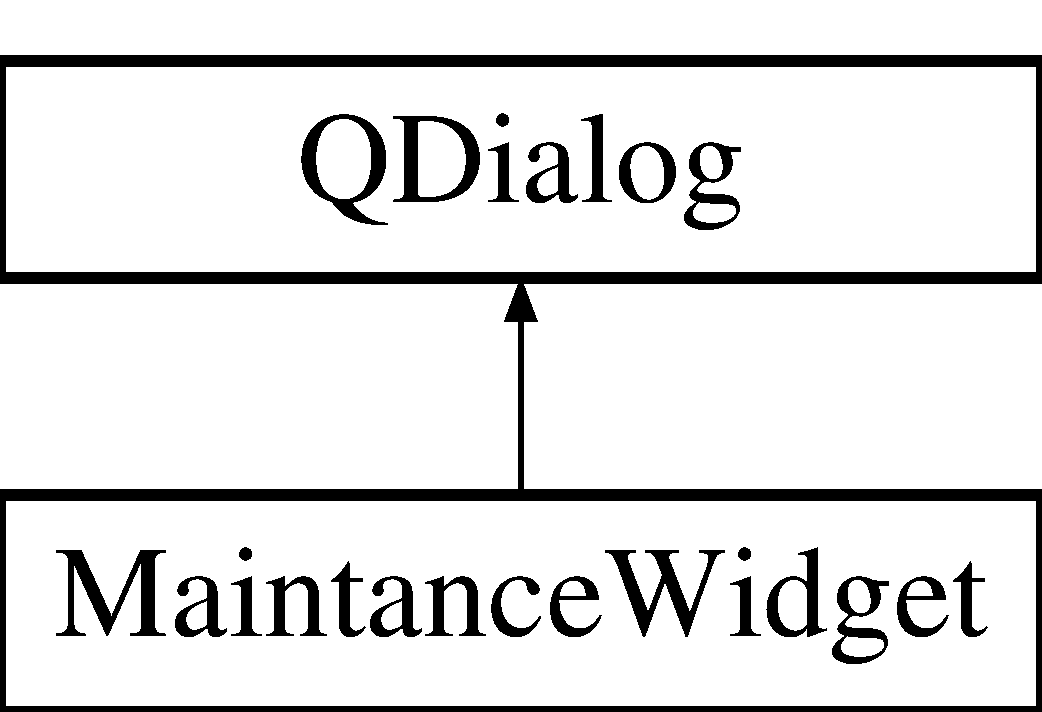
\includegraphics[height=2.000000cm]{classMaintanceWidget}
\end{center}
\end{figure}
\subsubsection*{Signals}
\begin{DoxyCompactItemize}
\item 
void \mbox{\hyperlink{classMaintanceWidget_a311671167a33d7d84a105c5b68c3c783}{trouble\+Solved}} (int trouble\+Index)
\item 
void \mbox{\hyperlink{classMaintanceWidget_a016a9e2ad10ba518b29ac0bf336d8b97}{maintance\+Closed}} (Q\+List$<$ \mbox{\hyperlink{classMaintanceElement}{Maintance\+Element}} $>$ elem\+List)
\item 
void \mbox{\hyperlink{classMaintanceWidget_a94a81d4c917de6cc0dba1135ab3be43e}{tutorial\+Request}} (int trouble\+Index)
\end{DoxyCompactItemize}
\subsubsection*{Public Member Functions}
\begin{DoxyCompactItemize}
\item 
\mbox{\hyperlink{classMaintanceWidget_a8e8a76199a50d91c200eb1d7dcc66a14}{Maintance\+Widget}} (Q\+Widget $\ast$parent=0)
\item 
\mbox{\hyperlink{classMaintanceWidget_ad824060037187de4a61a24ce2e393ca0}{$\sim$\+Maintance\+Widget}} ()
\item 
void \mbox{\hyperlink{classMaintanceWidget_a46dbe90c80f405b594f2998a10a548db}{clear\+Text}} ()
\item 
void \mbox{\hyperlink{classMaintanceWidget_a32f98e1e9388b400f9b04e2fa94e8ef8}{set\+Elemets}} (Q\+List$<$ \mbox{\hyperlink{classMaintanceElement}{Maintance\+Element}} $>$ elem\+List)
\end{DoxyCompactItemize}
\subsubsection*{Protected Member Functions}
\begin{DoxyCompactItemize}
\item 
void \mbox{\hyperlink{classMaintanceWidget_ac88ccb3da3c15f85575eb5d973004827}{change\+Event}} (Q\+Event $\ast$event)
\end{DoxyCompactItemize}
\subsubsection*{Private Slots}
\begin{DoxyCompactItemize}
\item 
void \mbox{\hyperlink{classMaintanceWidget_ae0e57574f94ec4b744247d15ff8a4891}{solved}} ()
\item 
void \mbox{\hyperlink{classMaintanceWidget_a239e4ddf537bfc43124ba4688fe285d0}{close\+Window}} ()
\item 
void \mbox{\hyperlink{classMaintanceWidget_adc20de8af45f910289c60d1f6656e783}{call\+Tutorial}} ()
\end{DoxyCompactItemize}
\subsubsection*{Private Attributes}
\begin{DoxyCompactItemize}
\item 
Ui\+::\+Maintance\+Widget $\ast$ \mbox{\hyperlink{classMaintanceWidget_a6a78c78ed723107e438c0919d1feae00}{ui}}
\item 
Q\+List$<$ \mbox{\hyperlink{classMaintanceElement}{Maintance\+Element}} $>$ \mbox{\hyperlink{classMaintanceWidget_a9c9003f07e28f258c99b996c3c02da45}{maintance\+List}}
\end{DoxyCompactItemize}


\subsubsection{Constructor \& Destructor Documentation}
\mbox{\Hypertarget{classMaintanceWidget_a8e8a76199a50d91c200eb1d7dcc66a14}\label{classMaintanceWidget_a8e8a76199a50d91c200eb1d7dcc66a14}} 
\index{Maintance\+Widget@{Maintance\+Widget}!Maintance\+Widget@{Maintance\+Widget}}
\index{Maintance\+Widget@{Maintance\+Widget}!Maintance\+Widget@{Maintance\+Widget}}
{\footnotesize\ttfamily Maintance\+Widget\+::\texorpdfstring{Maintance\+Widget}{MaintanceWidget} (\begin{DoxyParamCaption}\item[{Q\+Widget $\ast$}]{parent = {\ttfamily 0} }\end{DoxyParamCaption})\hspace{0.3cm}{\ttfamily [explicit]}} - standard Q\+Widget constructor. Used to create connections from buttons to functions.

\mbox{\Hypertarget{classMaintanceWidget_ad824060037187de4a61a24ce2e393ca0}\label{classMaintanceWidget_ad824060037187de4a61a24ce2e393ca0}} 
\index{Maintance\+Widget@{Maintance\+Widget}!````~Maintance\+Widget@{$\sim$\+Maintance\+Widget}}
\index{````~Maintance\+Widget@{$\sim$\+Maintance\+Widget}!Maintance\+Widget@{Maintance\+Widget}}
{\footnotesize\ttfamily Maintance\+Widget\+::\texorpdfstring{$\sim$\+Maintance\+Widget}{~MaintanceWidget} (\begin{DoxyParamCaption}{ }\end{DoxyParamCaption})} - standard Q\+Widget destructor.

\subsubsection{Member Function Documentation}
\mbox{\Hypertarget{classMaintanceWidget_adc20de8af45f910289c60d1f6656e783}\label{classMaintanceWidget_adc20de8af45f910289c60d1f6656e783}} 
\index{Maintance\+Widget@{Maintance\+Widget}!call\+Tutorial@{call\+Tutorial}}
\index{call\+Tutorial@{call\+Tutorial}!Maintance\+Widget@{Maintance\+Widget}}
{\footnotesize\ttfamily void Maintance\+Widget\+::\texorpdfstring{call\+Tutorial}{callTutorial} (\begin{DoxyParamCaption}{ }\end{DoxyParamCaption})\hspace{0.3cm}{\ttfamily [private]}, {\ttfamily [slot]}} - function created show (in some way) tutorial how to made maintenance for machine. It is not finished.

\mbox{\Hypertarget{classMaintanceWidget_ac88ccb3da3c15f85575eb5d973004827}\label{classMaintanceWidget_ac88ccb3da3c15f85575eb5d973004827}} 
\index{Maintance\+Widget@{Maintance\+Widget}!change\+Event@{change\+Event}}
\index{change\+Event@{change\+Event}!Maintance\+Widget@{Maintance\+Widget}}
{\footnotesize\ttfamily void Maintance\+Widget\+::\texorpdfstring{change\+Event}{\texorpdfstring{change\+Event}{changeEvent}} (\begin{DoxyParamCaption}\item[{Q\+Event $\ast$}]{event }\end{DoxyParamCaption})\hspace{0.3cm}{\ttfamily [protected]}} - reimplementation of default event for Q\+Dialog to enable user interface translation. Function called automatically.

\mbox{\Hypertarget{classMaintanceWidget_a46dbe90c80f405b594f2998a10a548db}\label{classMaintanceWidget_a46dbe90c80f405b594f2998a10a548db}} 
\index{Maintance\+Widget@{Maintance\+Widget}!clear\+Text@{clear\+Text}}
\index{clear\+Text@{clear\+Text}!Maintance\+Widget@{Maintance\+Widget}}
{\footnotesize\ttfamily void Maintance\+Widget\+::\texorpdfstring{clear\+Text}{clearText} (\begin{DoxyParamCaption}{ }\end{DoxyParamCaption})} - function used to  Q\+List\+Widget (remove all items).

\mbox{\Hypertarget{classMaintanceWidget_a239e4ddf537bfc43124ba4688fe285d0}\label{classMaintanceWidget_a239e4ddf537bfc43124ba4688fe285d0}} 
\index{Maintance\+Widget@{Maintance\+Widget}!close\+Window@{close\+Window}}
\index{close\+Window@{close\+Window}!Maintance\+Widget@{Maintance\+Widget}}
{\footnotesize\ttfamily void Maintance\+Widget\+::\texorpdfstring{close\+Window}{closeWindow} (\begin{DoxyParamCaption}{ }\end{DoxyParamCaption})\hspace{0.3cm}{\ttfamily [private]}, {\ttfamily [slot]}} - used to hide Q\+Dialog.

\mbox{\Hypertarget{classMaintanceWidget_a016a9e2ad10ba518b29ac0bf336d8b97}\label{classMaintanceWidget_a016a9e2ad10ba518b29ac0bf336d8b97}} 
\index{Maintance\+Widget@{Maintance\+Widget}!maintance\+Closed@{maintance\+Closed}}
\index{maintance\+Closed@{maintance\+Closed}!Maintance\+Widget@{Maintance\+Widget}}
{\footnotesize\ttfamily void Maintance\+Widget\+::\texorpdfstring{maintance\+Closed}{maintanceClosed} (\begin{DoxyParamCaption}\item[{Q\+List$<$ \mbox{\hyperlink{classMaintanceElement}{Maintance\+Element}} $>$}]{elem\+List }\end{DoxyParamCaption})\hspace{0.3cm}{\ttfamily [signal]}} - signal what emits on window hide. Parameter send \hyperlink{classMaintanceWidget_a9c9003f07e28f258c99b996c3c02da45}{maintance\+List} to signal handler.

\mbox{\Hypertarget{classMaintanceWidget_a32f98e1e9388b400f9b04e2fa94e8ef8}\label{classMaintanceWidget_a32f98e1e9388b400f9b04e2fa94e8ef8}} 
\index{Maintance\+Widget@{Maintance\+Widget}!set\+Elemets@{set\+Elemets}}
\index{set\+Elemets@{set\+Elemets}!Maintance\+Widget@{Maintance\+Widget}}
{\footnotesize\ttfamily void Maintance\+Widget\+::\texorpdfstring{set\+Elemets}{setElemets} (\begin{DoxyParamCaption}\item[{Q\+List$<$ \mbox{\hyperlink{classMaintanceElement}{Maintance\+Element}} $>$}]{elem\+List }\end{DoxyParamCaption})} - function which used to fill list\+Widget with maintenance elements and append \textit{elem\+List} to \hyperlink{classMaintanceWidget_a9c9003f07e28f258c99b996c3c02da45}{maintance\+List}. 

\mbox{\Hypertarget{classMaintanceWidget_ae0e57574f94ec4b744247d15ff8a4891}\label{classMaintanceWidget_ae0e57574f94ec4b744247d15ff8a4891}} 
\index{Maintance\+Widget@{Maintance\+Widget}!solved@{solved}}
\index{solved@{solved}!Maintance\+Widget@{Maintance\+Widget}}
{\footnotesize\ttfamily void Maintance\+Widget\+::\texorpdfstring{solved}{solved} (\begin{DoxyParamCaption}{ }\end{DoxyParamCaption})\hspace{0.3cm}{\ttfamily [private]}, {\ttfamily [slot]}} - function to remove selected at \textit{list\+Widget} item from \hyperlink{classMaintanceWidget_a9c9003f07e28f258c99b996c3c02da45}{maintance\+List} and from \textit{list\+Widget}. Also this function emit \hyperlink{classMaintanceWidget_a311671167a33d7d84a105c5b68c3c783}{trouble\+Solved}(...) signal with index at list to handle at parent object.

\mbox{\Hypertarget{classMaintanceWidget_a311671167a33d7d84a105c5b68c3c783}\label{classMaintanceWidget_a311671167a33d7d84a105c5b68c3c783}} 
\index{Maintance\+Widget@{Maintance\+Widget}!trouble\+Solved@{trouble\+Solved}}
\index{trouble\+Solved@{trouble\+Solved}!Maintance\+Widget@{Maintance\+Widget}}
{\footnotesize\ttfamily void Maintance\+Widget\+::\texorpdfstring{trouble\+Solved}{troubleSolved} (\begin{DoxyParamCaption}\item[{int}]{trouble\+Index }\end{DoxyParamCaption})\hspace{0.3cm}{\ttfamily [signal]}} - signal which handle at parent object (request redirected to \hyperlink{classMaintanceDialog_a3958b309d854fcd5baf39fc166a6b5f6}{solve\+Item}(...)) to change list of maintenance items at file system.

\mbox{\Hypertarget{classMaintanceWidget_a94a81d4c917de6cc0dba1135ab3be43e}\label{classMaintanceWidget_a94a81d4c917de6cc0dba1135ab3be43e}} 
\index{Maintance\+Widget@{Maintance\+Widget}!tutorial\+Request@{tutorial\+Request}}
\index{tutorial\+Request@{tutorial\+Request}!Maintance\+Widget@{Maintance\+Widget}}
{\footnotesize\ttfamily void Maintance\+Widget\+::\texorpdfstring{tutorial\+Request}{tutorialRequest} (\begin{DoxyParamCaption}\item[{int}]{trouble\+Index }\end{DoxyParamCaption})\hspace{0.3cm}{\ttfamily [signal]}} - signal which emitted by \hyperlink{classMaintanceWidget_adc20de8af45f910289c60d1f6656e783}{call\+Tutorial}(...) function. Handled in parent object (handler is not created at present moment).



\subsubsection{Member Data Documentation}
\mbox{\Hypertarget{classMaintanceWidget_a9c9003f07e28f258c99b996c3c02da45}\label{classMaintanceWidget_a9c9003f07e28f258c99b996c3c02da45}} 
\index{Maintance\+Widget@{Maintance\+Widget}!maintance\+List@{maintance\+List}}
\index{maintance\+List@{maintance\+List}!Maintance\+Widget@{Maintance\+Widget}}
{\footnotesize\ttfamily Q\+List$<$\mbox{\hyperlink{classMaintanceElement}{Maintance\+Element}}$>$ Maintance\+Widget\+::\texorpdfstring{maintance\+List}{maintanceList}\hspace{0.3cm}{\ttfamily [private]}}


The documentation for this class was generated from the following files\+:\begin{DoxyCompactItemize}
\item 
\mbox{\hyperlink{maintancewidget_8h}{maintancewidget.\+h}}\item 
\mbox{\hyperlink{maintancewidget_8cpp}{maintancewidget.\+cpp}}\end{DoxyCompactItemize}
\newpage
\hypertarget{classMainWindow}{}\subsection{Main\+Window Class Reference}
\label{classMainWindow}\index{Main\+Window@{Main\+Window}}


{\ttfamily \#include $<$mainwindow.\+h$>$}

Inheritance diagram for Main\+Window\+:\begin{figure}[H]
\begin{center}
\leavevmode
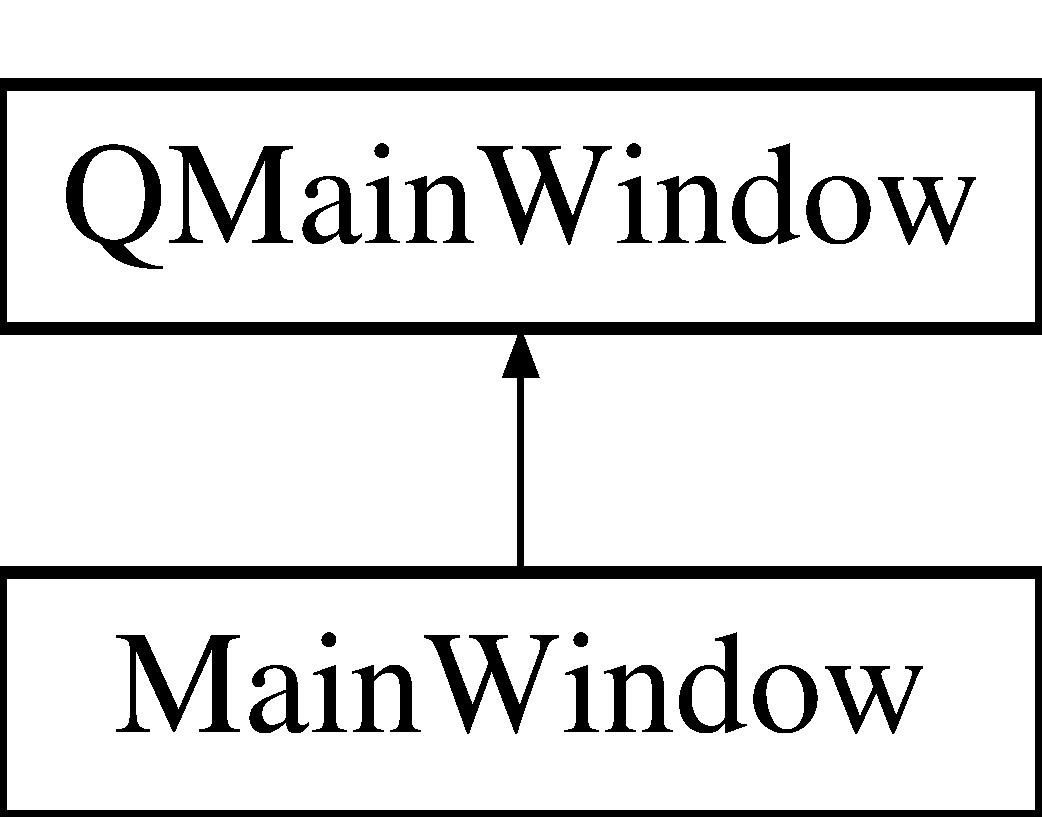
\includegraphics[height=2.000000cm]{classMainWindow}
\end{center}
\end{figure}
\subsubsection*{Public Member Functions}
\begin{DoxyCompactItemize}
\item 
\mbox{\hyperlink{classMainWindow_a8b244be8b7b7db1b08de2a2acb9409db}{Main\+Window}} (Q\+Widget $\ast$parent=0)
\item 
\mbox{\hyperlink{classMainWindow_ae98d00a93bc118200eeef9f9bba1dba7}{$\sim$\+Main\+Window}} ()
\item 
void \mbox{\hyperlink{classMainWindow_a960f1895aaeb4e7a6828a5eeb70b5cf1}{master\+Code\+Check}} ()
\item 
void \mbox{\hyperlink{classMainWindow_a339962b149079e9cdb8928c5528113ea}{user\+Login}} ()
\end{DoxyCompactItemize}
\subsubsection*{Public Attributes}
\begin{DoxyCompactItemize}
\item 
\mbox{\hyperlink{classExitDialog_a750dfbbef3dec32bec821122ee7b910c}{Exit\+Dialog\+::\+Exit\+Code}} \mbox{\hyperlink{classMainWindow_a40a55ca38922e5e3c0f3ee92584b72f1}{exit\+Code}}
\end{DoxyCompactItemize}
\subsubsection*{Protected Member Functions}
\begin{DoxyCompactItemize}
\item 
virtual void \mbox{\hyperlink{classMainWindow_af925e4c05190e6672fbc4a171b0016b8}{resize\+Event}} (Q\+Resize\+Event $\ast$e)
\item 
void \mbox{\hyperlink{classMainWindow_a332a98884795104796ad57e49943134c}{show\+Event}} (Q\+Show\+Event $\ast$ev)
\item 
bool \mbox{\hyperlink{classMainWindow_a53b218282f3d113b2aec441a3313f472}{event\+Filter}} (Q\+Object $\ast$obj, Q\+Event $\ast$ev)
\item 
void \mbox{\hyperlink{classMainWindow_ac7c881667b4ba4986b5a0030452ee3f0}{change\+Event}} (Q\+Event $\ast$event)
\end{DoxyCompactItemize}
\subsubsection*{Private Slots}
\begin{DoxyCompactItemize}
\item 
void \mbox{\hyperlink{classMainWindow_a9fc9d44f9d830e8f49d7052a88483d01}{zero\+Start}} ()
\item 
void \mbox{\hyperlink{classMainWindow_ac9861b0745a5505aaa5a6005a940e763}{heads\+Init}} ()
\item 
void \mbox{\hyperlink{classMainWindow_a5e694c3f8a020709ebd7e7e244655960}{watch\+Dog\+Timeout}} ()
\item 
void \mbox{\hyperlink{classMainWindow_ae823008e53cce4636c1776d86c946cf5}{head\+Setting\+Request}} (int index)
\item 
void \mbox{\hyperlink{classMainWindow_a867f15b0c134336e5477e80673f1903d}{indexer\+Lift\+Setting\+Request}} ()
\item 
void \mbox{\hyperlink{classMainWindow_a12f17b40fbfc42aa601dbfc583ea93dd}{general\+Setting\+Dialog\+Request}} ()
\item 
void \mbox{\hyperlink{classMainWindow_a2b45d2c72983565a0e0036054db498ce}{change\+Head\+No}} (int index)
\item 
void \mbox{\hyperlink{classMainWindow_a2d957a5c154ebce97484e8aa7fa2abb3}{reset\+Machine}} ()
\item 
void \mbox{\hyperlink{classMainWindow_a98db3a076389e7afc0f51bf980566851}{get\+Serial\+Data}} (\mbox{\hyperlink{serialport_8h_a2331c0232719069f0bce03c249d2eec6}{Mod\+Data}} mod\+Data)
\item 
void \mbox{\hyperlink{classMainWindow_ae1cb8ad1d2de77b497e219ce293cb053}{get\+Udp\+Data}} (Q\+Byte\+Array data)
\item 
void \mbox{\hyperlink{classMainWindow_a58b01de5b75f610847c9ad2b1c58165b}{get\+Head\+Color}} (int index, Q\+Color color)
\item 
void \mbox{\hyperlink{classMainWindow_ab019f061b5bdeba9339746d5092107ac}{get\+Head\+Param}} (int index, Q\+Byte\+Array h\+Param\+Arr)
\item 
void \mbox{\hyperlink{classMainWindow_a10d8d19caf33169392e8f4e8373fbb73}{get\+All\+Head\+Param}} (int index, Q\+Byte\+Array h\+Param\+Arr)
\item 
void \mbox{\hyperlink{classMainWindow_aa4e6c4af31a8f3189e2f6d6b945796b8}{get\+Head\+Command}} (int index, Q\+Byte\+Array command\+Arr)
\item 
void \mbox{\hyperlink{classMainWindow_ad5c320ccd4b6df9c8b4aec7914803b82}{get\+Head\+Activ\+Command}} (Q\+Byte\+Array command\+Arr)
\item 
void \mbox{\hyperlink{classMainWindow_a7f0e94461843c006389d792048c6b2d1}{get\+Cycles\+Command}} (Q\+Byte\+Array command\+Arr)
\item 
void \mbox{\hyperlink{classMainWindow_a7c2d999fc817728b31dccaaa1e72bd43}{get\+Load\+State}} (int index, \mbox{\hyperlink{headform_8h_a56d194976643934b3332b3f99d82490d}{Load\+State}} state)
\item 
void \mbox{\hyperlink{classMainWindow_a5c6f8757a262535d243b6f481ceb570b}{get\+Indexer\+Param}} (Q\+Byte\+Array indexer\+Param\+Arr)
\item 
void \mbox{\hyperlink{classMainWindow_a2dc63192aa7ff54dfc64e8308712c287}{get\+Machine\+Param}} (Q\+Byte\+Array machine\+Param\+Arr)
\item 
void \mbox{\hyperlink{classMainWindow_a1da3e0b195babf250e071baca42b16b3}{get\+Step\+Delay\+Time}} (double arg1)
\item 
void \mbox{\hyperlink{classMainWindow_a98097440e933cbc9a5080320e230c124}{get\+Direction}} (int direction)
\item 
void \mbox{\hyperlink{classMainWindow_aeee3b80eb69746981c80032d8992ed46}{set\+Unload\+State}} (bool state)
\item 
void \mbox{\hyperlink{classMainWindow_a65683f9a3748cd4f783daf2f57b4f318}{get\+Lift\+Param}} (Q\+Byte\+Array lift\+Param\+Arr)
\item 
void \mbox{\hyperlink{classMainWindow_a9da44a03d4e720dba6a3d63f7aa22ea5}{get\+Lift\+Offcet}} (double arg1)
\item 
void \mbox{\hyperlink{classMainWindow_a11a73a8f479b8952951f29df988ff2c3}{get\+Lift\+Distance}} (float distance)
\item 
void \mbox{\hyperlink{classMainWindow_a4f4ada31d5edeadf6450a1cf952182c0}{get\+Index\+Lift\+Sett\+Comm}} (Q\+Byte\+Array command\+Arr)
\item 
void \mbox{\hyperlink{classMainWindow_aefe64936a5d347902ba7d9438294dab8}{get\+Index\+Lift\+Command}} (Q\+Byte\+Array command\+Arr)
\item 
void \mbox{\hyperlink{classMainWindow_a3dfd3ec74dbf6a8bbef327aab4c88de4}{get\+Machine\+Command}} (Q\+Byte\+Array command\+Arr)
\item 
void \mbox{\hyperlink{classMainWindow_a477250c56749d4db7cf5d94ea30145cf}{get\+Serial\+Setting}} (\mbox{\hyperlink{structComSettings}{Com\+Settings}} com\+Sett)
\item 
void \mbox{\hyperlink{classMainWindow_a5782e86aacd3c157412821fae13c85fb}{get\+Email\+Settings}} (\mbox{\hyperlink{structEmailSettings}{Email\+Settings}} email\+Sett)
\item 
void \mbox{\hyperlink{classMainWindow_ace96362adad45fba8ba98fa834ddb7f2}{get\+Veiw\+Settings}} (int st\+Sheet\+Index)
\item 
void \mbox{\hyperlink{classMainWindow_a96b56bd09db03ada451752dbbf993f12}{get\+Lang\+File}} (int lang\+Index)
\item 
void \mbox{\hyperlink{classMainWindow_a6390c39f77f17e86c59a4c8f8bf0e607}{service\+State\+Change}} ()
\item 
void \mbox{\hyperlink{classMainWindow_adb19747ac0579b12b268675c948dadeb}{exit\+Program}} (bool restart=false)
\item 
void \mbox{\hyperlink{classMainWindow_ae527207542e0df2d2aaa73d56fff003f}{save\+Job}} ()
\item 
void \mbox{\hyperlink{classMainWindow_afa9412b024ccb24c4299cc4ce4dd5327}{load\+Job}} ()
\item 
void \mbox{\hyperlink{classMainWindow_a5adab082570604b67b5a36479cc54121}{set\+Heads\+Position}} ()
\item 
void \mbox{\hyperlink{classMainWindow_a9ef526df9f964d8e10d8115a2cd10a28}{indexer\+Step\+Finish}} ()
\item 
void \mbox{\hyperlink{classMainWindow_a18d83d170a660644bb70fda6b28a2bc6}{start\+Print\+Process}} (bool auto\+Print)
\item 
void \mbox{\hyperlink{classMainWindow_a80282fbc6eb85c0f6594975e02a150a3}{stop\+Print\+Process}} ()
\item 
void \mbox{\hyperlink{classMainWindow_a5efe485c39e957ff3d4340328e4eb20d}{maintance\+Work\+Slot}} (bool enable)
\item 
void \mbox{\hyperlink{classMainWindow_ad8e2a953cbde0cc4ba7bc71567368029}{show\+Maintanance\+Widget}} ()
\item 
void \mbox{\hyperlink{classMainWindow_a1c07847e8f3adb976aa52cea3f032d7d}{set\+Icon\+Folder}} (int index)
\item 
void \mbox{\hyperlink{classMainWindow_aa08c1cb3f9e678d6af8f79dc2cc486d5}{set\+Back\+Ground}} (bool enable, bool request=false)
\item 
void \mbox{\hyperlink{classMainWindow_af9aa632b092ec3f2e86b62ceacc82a62}{update\+Time\+Slot}} ()
\end{DoxyCompactItemize}
\subsubsection*{Private Attributes}
\begin{DoxyCompactItemize}
\item 
Ui\+::\+Main\+Window $\ast$ \mbox{\hyperlink{classMainWindow_a35466a70ed47252a0191168126a352a5}{ui}}
\item 
Q\+List$<$ \mbox{\hyperlink{classHeadForm}{Head\+Form}} $\ast$ $>$ \mbox{\hyperlink{classMainWindow_aee1f0ef16a77d46e13672b5219cadef7}{head\+Button}}
\item 
Q\+List$<$ \mbox{\hyperlink{classHeadSettingButton}{Head\+Setting\+Button}} $\ast$ $>$ \mbox{\hyperlink{classMainWindow_a5fc117f7fb33eaa3bd4a40f63eb1d32c}{head\+Sett\+Button}}
\item 
\mbox{\hyperlink{classInfoWidget}{Info\+Widget}} $\ast$ \mbox{\hyperlink{classMainWindow_a1ec5a697ad1c0526e4979dd538d11f20}{info\+Widget}}
\item 
Q\+Settings $\ast$ \mbox{\hyperlink{classMainWindow_a4d8dbbb57b71b4fde207e465526a6753}{settings}}
\item 
Q\+Settings $\ast$ \mbox{\hyperlink{classMainWindow_a92c60042483f6bcdef44a4b06bec8795}{master\+Codes}}
\item 
\mbox{\hyperlink{classHeadSetting}{Head\+Setting}} \mbox{\hyperlink{classMainWindow_abfbbbda04b8875212b6c12d3bf6f94cb}{head\+Settings}}
\item 
\mbox{\hyperlink{classIndexerLiftSettings}{Indexer\+Lift\+Settings}} \mbox{\hyperlink{classMainWindow_ab8dfb97cd685ef6fb299506ddc2e6170}{indexer\+Lift\+Settings}}
\item 
\mbox{\hyperlink{classMachineSettings}{Machine\+Settings}} \mbox{\hyperlink{classMainWindow_ae8dd8666bcd48aebe9f7a00017dff875}{machine\+Settings}}
\item 
\mbox{\hyperlink{classGeneralSettingDialog}{General\+Setting\+Dialog}} $\ast$ \mbox{\hyperlink{classMainWindow_ac52bc1afdcda6200044e85a40de61c52}{general\+Setting\+Dialog}}
\item 
\mbox{\hyperlink{classSettingDialog}{Setting\+Dialog}} $\ast$ \mbox{\hyperlink{classMainWindow_ae13512af59f04b0fb3bf6bf3f8d4cca1}{head\+Setting\+Dialog}}
\item 
\mbox{\hyperlink{classIndexerSettingDialog}{Indexer\+Setting\+Dialog}} $\ast$ \mbox{\hyperlink{classMainWindow_ab0cf5f0fbfa991a1a6fe78ef34db6ac3}{indexer\+Lift\+Set\+Dialog}}
\item 
\mbox{\hyperlink{classSerialSettingsDialog}{Serial\+Settings\+Dialog}} $\ast$ \mbox{\hyperlink{classMainWindow_a5f2e9273d4144c9f5f63b68bbaa6b7b1}{serial\+Settings\+Dialog}}
\item 
\mbox{\hyperlink{classIndexerWidget}{Indexer\+Widget}} $\ast$ \mbox{\hyperlink{classMainWindow_a2a9bf85f8e206a2db53a4a01a3531367}{indexer}}
\item 
\mbox{\hyperlink{classMailSender}{Mail\+Sender}} $\ast$ \mbox{\hyperlink{classMainWindow_a69258924e6672d7a887839b5c327a0b1}{mail\+Sender}}
\item 
\mbox{\hyperlink{classUserSettingDialog}{User\+Setting\+Dialog}} $\ast$ \mbox{\hyperlink{classMainWindow_aac26d8e6ed8e1afe7405cddec279f3ae}{users\+Setting\+Dialog}}
\item 
\mbox{\hyperlink{classMaintanceDialog}{Maintance\+Dialog}} $\ast$ \mbox{\hyperlink{classMainWindow_a0a1edb572efa46ec0d2b938ed6ebf876}{maintance\+Dialog}}
\item 
\mbox{\hyperlink{classMaintanceWidget}{Maintance\+Widget}} $\ast$ \mbox{\hyperlink{classMainWindow_a932658effa63d92d234d9fe0be097f17}{maintance\+Widget}}
\item 
\mbox{\hyperlink{classCyclesDialog}{Cycles\+Dialog}} $\ast$ \mbox{\hyperlink{classMainWindow_ae3d19fe8260d3c71218159a3fbb07247}{cycle\+Dialog}}
\item 
\mbox{\hyperlink{classHeadActivationDialog}{Head\+Activation\+Dialog}} $\ast$ \mbox{\hyperlink{classMainWindow_ade9f7ec0590bb905ef05f36b5f1ff375}{head\+Act\+Dialog}}
\item 
\mbox{\hyperlink{classReprogramDialog}{Reprogram\+Dialog}} $\ast$ \mbox{\hyperlink{classMainWindow_a70160014215b6053d8bcd08f797c2d99}{reprogram\+Dialog}}
\item 
\mbox{\hyperlink{classSerialPort}{Serial\+Port}} $\ast$ \mbox{\hyperlink{classMainWindow_a5ff9608e15352bd8134510f71adec645}{com\+Port}}
\item 
\mbox{\hyperlink{classUdpSocket}{Udp\+Socket}} $\ast$ \mbox{\hyperlink{classMainWindow_a02e8becbdef8a4a64947536d83a5a0de}{udp\+Handler}}
\item 
Q\+Timer $\ast$ \mbox{\hyperlink{classMainWindow_ace7bf6dfd47ef0be2fd33e7bdfe12f45}{watch\+Dog}}
\item 
Q\+Timer $\ast$ \mbox{\hyperlink{classMainWindow_ad1c1f98b63a93fc70964304d1b0006be}{update\+Time}}
\item 
Q\+Time \mbox{\hyperlink{classMainWindow_a5c567ee1bf6cac065f7c1217a76dbb79}{time\+Program\+Start}}
\item 
Q\+Time \mbox{\hyperlink{classMainWindow_a42fcbf877e14a05140136a65fdfd70a8}{time\+Program\+End}}
\item 
Q\+Time \mbox{\hyperlink{classMainWindow_a22176130c60005fad11cbc01de405480}{time\+Working}}
\item 
Q\+String \mbox{\hyperlink{classMainWindow_a45573d099a3f1c9292c566b787168aec}{true\+Password}}
\item 
bool \mbox{\hyperlink{classMainWindow_aa8aa688516b17c3efab6a28caf771e58}{loged\+In\+Head\+Settings}}
\item 
bool \mbox{\hyperlink{classMainWindow_ac21c269cb5cfa4fdd078cb5ff8dc9633}{loged\+In\+Indexer}}
\item 
bool \mbox{\hyperlink{classMainWindow_a77f5ccbec73adcd6e9f759728d5b7432}{loged\+In\+General}}
\item 
bool \mbox{\hyperlink{classMainWindow_a5baddcb9fe93bad0e0cd3a2272b55209}{loged\+In\+Service}}
\item 
\mbox{\hyperlink{settings_8h_a017dd44e68049ffdd31500a8cd01ba68}{uint16\+\_\+t}} \mbox{\hyperlink{classMainWindow_ac825500f4c4298bc0d7d1dd2a8eeb92b}{heads\+Count}}
\item 
bool \mbox{\hyperlink{classMainWindow_a1a1b01298c3c5e551156b42979f1424f}{need\+Complete\+Reset}}
\item 
int \mbox{\hyperlink{classMainWindow_ac9a80bbcf3f47b2e943482dcbe2a22b6}{indexer\+Cycles\+Session}}
\item 
int \mbox{\hyperlink{classMainWindow_abac49512503987bde5163902aea88ff8}{indexer\+Cycles\+All}}
\item 
int \mbox{\hyperlink{classMainWindow_ae9d373f6b3527dd622b61056db5960ca}{rag\+Session\+Count}}
\item 
int \mbox{\hyperlink{classMainWindow_a66a1308d51a2a1fb60ab4cdbc35c60f6}{rag\+All\+Count}}
\item 
\mbox{\hyperlink{settings_8h_a4196118492a3b1493c81f250e90af775}{uint32\+\_\+t}} \mbox{\hyperlink{classMainWindow_adc85b6b79621bbed931579da596287ef}{rag\+All\+Count\+Reg}}
\item 
int \mbox{\hyperlink{classMainWindow_a29f41984f291911f0bbdd68830b2d9e0}{rag\+At\+Head\+Count}}
\item 
bool \mbox{\hyperlink{classMainWindow_ad1264be93d1c2e447f834cd430337f8f}{auto\+Print\+Enabled}}
\item 
Q\+String \mbox{\hyperlink{classMainWindow_a898b67827c6cce8017f39157be449a6c}{user\+Name}}
\item 
\mbox{\hyperlink{classRegister}{Register}} $\ast$ \mbox{\hyperlink{classMainWindow_aead190b1b4ca3ce95076274ab2ae6f84}{registers}}
\item 
Q\+Translator \mbox{\hyperlink{classMainWindow_a8e829b3590ccdeeada42625415afc6f3}{translator}}
\item 
Q\+String\+List \mbox{\hyperlink{classMainWindow_aec7acc53aaf3436cc02ed0066a72b5a8}{head\+Styles\+Str}}
\end{DoxyCompactItemize}


\subsubsection{Constructor \& Destructor Documentation}
\mbox{\Hypertarget{classMainWindow_a8b244be8b7b7db1b08de2a2acb9409db}\label{classMainWindow_a8b244be8b7b7db1b08de2a2acb9409db}} 
\index{Main\+Window@{Main\+Window}!Main\+Window@{Main\+Window}}
\index{Main\+Window@{Main\+Window}!Main\+Window@{Main\+Window}}
\paragraph{\texorpdfstring{Main\+Window()}{MainWindow()}}
{\footnotesize\ttfamily Main\+Window\+::\+Main\+Window (\begin{DoxyParamCaption}\item[{Q\+Widget $\ast$}]{parent = {\ttfamily 0} }\end{DoxyParamCaption})\hspace{0.3cm}{\ttfamily [explicit]}}

\mbox{\Hypertarget{classMainWindow_ae98d00a93bc118200eeef9f9bba1dba7}\label{classMainWindow_ae98d00a93bc118200eeef9f9bba1dba7}} 
\index{Main\+Window@{Main\+Window}!````~Main\+Window@{$\sim$\+Main\+Window}}
\index{````~Main\+Window@{$\sim$\+Main\+Window}!Main\+Window@{Main\+Window}}
\paragraph{\texorpdfstring{$\sim$\+Main\+Window()}{~MainWindow()}}
{\footnotesize\ttfamily Main\+Window\+::$\sim$\+Main\+Window (\begin{DoxyParamCaption}{ }\end{DoxyParamCaption})}



\subsubsection{Member Function Documentation}
\mbox{\Hypertarget{classMainWindow_ac7c881667b4ba4986b5a0030452ee3f0}\label{classMainWindow_ac7c881667b4ba4986b5a0030452ee3f0}} 
\index{Main\+Window@{Main\+Window}!change\+Event@{change\+Event}}
\index{change\+Event@{change\+Event}!Main\+Window@{Main\+Window}}
\paragraph{\texorpdfstring{change\+Event()}{changeEvent()}}
{\footnotesize\ttfamily void Main\+Window\+::change\+Event (\begin{DoxyParamCaption}\item[{Q\+Event $\ast$}]{event }\end{DoxyParamCaption})\hspace{0.3cm}{\ttfamily [protected]}}

\mbox{\Hypertarget{classMainWindow_a2b45d2c72983565a0e0036054db498ce}\label{classMainWindow_a2b45d2c72983565a0e0036054db498ce}} 
\index{Main\+Window@{Main\+Window}!change\+Head\+No@{change\+Head\+No}}
\index{change\+Head\+No@{change\+Head\+No}!Main\+Window@{Main\+Window}}
\paragraph{\texorpdfstring{change\+Head\+No}{changeHeadNo}}
{\footnotesize\ttfamily void Main\+Window\+::change\+Head\+No (\begin{DoxyParamCaption}\item[{int}]{index }\end{DoxyParamCaption})\hspace{0.3cm}{\ttfamily [private]}, {\ttfamily [slot]}}

\mbox{\Hypertarget{classMainWindow_a53b218282f3d113b2aec441a3313f472}\label{classMainWindow_a53b218282f3d113b2aec441a3313f472}} 
\index{Main\+Window@{Main\+Window}!event\+Filter@{event\+Filter}}
\index{event\+Filter@{event\+Filter}!Main\+Window@{Main\+Window}}
\paragraph{\texorpdfstring{event\+Filter()}{eventFilter()}}
{\footnotesize\ttfamily bool Main\+Window\+::event\+Filter (\begin{DoxyParamCaption}\item[{Q\+Object $\ast$}]{obj,  }\item[{Q\+Event $\ast$}]{ev }\end{DoxyParamCaption})\hspace{0.3cm}{\ttfamily [protected]}}

\mbox{\Hypertarget{classMainWindow_adb19747ac0579b12b268675c948dadeb}\label{classMainWindow_adb19747ac0579b12b268675c948dadeb}} 
\index{Main\+Window@{Main\+Window}!exit\+Program@{exit\+Program}}
\index{exit\+Program@{exit\+Program}!Main\+Window@{Main\+Window}}
\paragraph{\texorpdfstring{exit\+Program}{exitProgram}}
{\footnotesize\ttfamily void Main\+Window\+::exit\+Program (\begin{DoxyParamCaption}\item[{bool}]{restart = {\ttfamily false} }\end{DoxyParamCaption})\hspace{0.3cm}{\ttfamily [private]}, {\ttfamily [slot]}}

\mbox{\Hypertarget{classMainWindow_a12f17b40fbfc42aa601dbfc583ea93dd}\label{classMainWindow_a12f17b40fbfc42aa601dbfc583ea93dd}} 
\index{Main\+Window@{Main\+Window}!general\+Setting\+Dialog\+Request@{general\+Setting\+Dialog\+Request}}
\index{general\+Setting\+Dialog\+Request@{general\+Setting\+Dialog\+Request}!Main\+Window@{Main\+Window}}
\paragraph{\texorpdfstring{general\+Setting\+Dialog\+Request}{generalSettingDialogRequest}}
{\footnotesize\ttfamily void Main\+Window\+::general\+Setting\+Dialog\+Request (\begin{DoxyParamCaption}{ }\end{DoxyParamCaption})\hspace{0.3cm}{\ttfamily [private]}, {\ttfamily [slot]}}

\mbox{\Hypertarget{classMainWindow_a10d8d19caf33169392e8f4e8373fbb73}\label{classMainWindow_a10d8d19caf33169392e8f4e8373fbb73}} 
\index{Main\+Window@{Main\+Window}!get\+All\+Head\+Param@{get\+All\+Head\+Param}}
\index{get\+All\+Head\+Param@{get\+All\+Head\+Param}!Main\+Window@{Main\+Window}}
\paragraph{\texorpdfstring{get\+All\+Head\+Param}{getAllHeadParam}}
{\footnotesize\ttfamily void Main\+Window\+::get\+All\+Head\+Param (\begin{DoxyParamCaption}\item[{int}]{index,  }\item[{Q\+Byte\+Array}]{h\+Param\+Arr }\end{DoxyParamCaption})\hspace{0.3cm}{\ttfamily [private]}, {\ttfamily [slot]}}

\mbox{\Hypertarget{classMainWindow_a7f0e94461843c006389d792048c6b2d1}\label{classMainWindow_a7f0e94461843c006389d792048c6b2d1}} 
\index{Main\+Window@{Main\+Window}!get\+Cycles\+Command@{get\+Cycles\+Command}}
\index{get\+Cycles\+Command@{get\+Cycles\+Command}!Main\+Window@{Main\+Window}}
\paragraph{\texorpdfstring{get\+Cycles\+Command}{getCyclesCommand}}
{\footnotesize\ttfamily void Main\+Window\+::get\+Cycles\+Command (\begin{DoxyParamCaption}\item[{Q\+Byte\+Array}]{command\+Arr }\end{DoxyParamCaption})\hspace{0.3cm}{\ttfamily [private]}, {\ttfamily [slot]}}

\mbox{\Hypertarget{classMainWindow_a98097440e933cbc9a5080320e230c124}\label{classMainWindow_a98097440e933cbc9a5080320e230c124}} 
\index{Main\+Window@{Main\+Window}!get\+Direction@{get\+Direction}}
\index{get\+Direction@{get\+Direction}!Main\+Window@{Main\+Window}}
\paragraph{\texorpdfstring{get\+Direction}{getDirection}}
{\footnotesize\ttfamily void Main\+Window\+::get\+Direction (\begin{DoxyParamCaption}\item[{int}]{direction }\end{DoxyParamCaption})\hspace{0.3cm}{\ttfamily [private]}, {\ttfamily [slot]}}

\mbox{\Hypertarget{classMainWindow_a5782e86aacd3c157412821fae13c85fb}\label{classMainWindow_a5782e86aacd3c157412821fae13c85fb}} 
\index{Main\+Window@{Main\+Window}!get\+Email\+Settings@{get\+Email\+Settings}}
\index{get\+Email\+Settings@{get\+Email\+Settings}!Main\+Window@{Main\+Window}}
\paragraph{\texorpdfstring{get\+Email\+Settings}{getEmailSettings}}
{\footnotesize\ttfamily void Main\+Window\+::get\+Email\+Settings (\begin{DoxyParamCaption}\item[{\mbox{\hyperlink{structEmailSettings}{Email\+Settings}}}]{email\+Sett }\end{DoxyParamCaption})\hspace{0.3cm}{\ttfamily [private]}, {\ttfamily [slot]}}

\mbox{\Hypertarget{classMainWindow_ad5c320ccd4b6df9c8b4aec7914803b82}\label{classMainWindow_ad5c320ccd4b6df9c8b4aec7914803b82}} 
\index{Main\+Window@{Main\+Window}!get\+Head\+Activ\+Command@{get\+Head\+Activ\+Command}}
\index{get\+Head\+Activ\+Command@{get\+Head\+Activ\+Command}!Main\+Window@{Main\+Window}}
\paragraph{\texorpdfstring{get\+Head\+Activ\+Command}{getHeadActivCommand}}
{\footnotesize\ttfamily void Main\+Window\+::get\+Head\+Activ\+Command (\begin{DoxyParamCaption}\item[{Q\+Byte\+Array}]{command\+Arr }\end{DoxyParamCaption})\hspace{0.3cm}{\ttfamily [private]}, {\ttfamily [slot]}}

\mbox{\Hypertarget{classMainWindow_a58b01de5b75f610847c9ad2b1c58165b}\label{classMainWindow_a58b01de5b75f610847c9ad2b1c58165b}} 
\index{Main\+Window@{Main\+Window}!get\+Head\+Color@{get\+Head\+Color}}
\index{get\+Head\+Color@{get\+Head\+Color}!Main\+Window@{Main\+Window}}
\paragraph{\texorpdfstring{get\+Head\+Color}{getHeadColor}}
{\footnotesize\ttfamily void Main\+Window\+::get\+Head\+Color (\begin{DoxyParamCaption}\item[{int}]{index,  }\item[{Q\+Color}]{color }\end{DoxyParamCaption})\hspace{0.3cm}{\ttfamily [private]}, {\ttfamily [slot]}}

\mbox{\Hypertarget{classMainWindow_aa4e6c4af31a8f3189e2f6d6b945796b8}\label{classMainWindow_aa4e6c4af31a8f3189e2f6d6b945796b8}} 
\index{Main\+Window@{Main\+Window}!get\+Head\+Command@{get\+Head\+Command}}
\index{get\+Head\+Command@{get\+Head\+Command}!Main\+Window@{Main\+Window}}
\paragraph{\texorpdfstring{get\+Head\+Command}{getHeadCommand}}
{\footnotesize\ttfamily void Main\+Window\+::get\+Head\+Command (\begin{DoxyParamCaption}\item[{int}]{index,  }\item[{Q\+Byte\+Array}]{command\+Arr }\end{DoxyParamCaption})\hspace{0.3cm}{\ttfamily [private]}, {\ttfamily [slot]}}

\mbox{\Hypertarget{classMainWindow_ab019f061b5bdeba9339746d5092107ac}\label{classMainWindow_ab019f061b5bdeba9339746d5092107ac}} 
\index{Main\+Window@{Main\+Window}!get\+Head\+Param@{get\+Head\+Param}}
\index{get\+Head\+Param@{get\+Head\+Param}!Main\+Window@{Main\+Window}}
\paragraph{\texorpdfstring{get\+Head\+Param}{getHeadParam}}
{\footnotesize\ttfamily void Main\+Window\+::get\+Head\+Param (\begin{DoxyParamCaption}\item[{int}]{index,  }\item[{Q\+Byte\+Array}]{h\+Param\+Arr }\end{DoxyParamCaption})\hspace{0.3cm}{\ttfamily [private]}, {\ttfamily [slot]}}

\mbox{\Hypertarget{classMainWindow_a5c6f8757a262535d243b6f481ceb570b}\label{classMainWindow_a5c6f8757a262535d243b6f481ceb570b}} 
\index{Main\+Window@{Main\+Window}!get\+Indexer\+Param@{get\+Indexer\+Param}}
\index{get\+Indexer\+Param@{get\+Indexer\+Param}!Main\+Window@{Main\+Window}}
\paragraph{\texorpdfstring{get\+Indexer\+Param}{getIndexerParam}}
{\footnotesize\ttfamily void Main\+Window\+::get\+Indexer\+Param (\begin{DoxyParamCaption}\item[{Q\+Byte\+Array}]{indexer\+Param\+Arr }\end{DoxyParamCaption})\hspace{0.3cm}{\ttfamily [private]}, {\ttfamily [slot]}}

\mbox{\Hypertarget{classMainWindow_aefe64936a5d347902ba7d9438294dab8}\label{classMainWindow_aefe64936a5d347902ba7d9438294dab8}} 
\index{Main\+Window@{Main\+Window}!get\+Index\+Lift\+Command@{get\+Index\+Lift\+Command}}
\index{get\+Index\+Lift\+Command@{get\+Index\+Lift\+Command}!Main\+Window@{Main\+Window}}
\paragraph{\texorpdfstring{get\+Index\+Lift\+Command}{getIndexLiftCommand}}
{\footnotesize\ttfamily void Main\+Window\+::get\+Index\+Lift\+Command (\begin{DoxyParamCaption}\item[{Q\+Byte\+Array}]{command\+Arr }\end{DoxyParamCaption})\hspace{0.3cm}{\ttfamily [private]}, {\ttfamily [slot]}}

\mbox{\Hypertarget{classMainWindow_a4f4ada31d5edeadf6450a1cf952182c0}\label{classMainWindow_a4f4ada31d5edeadf6450a1cf952182c0}} 
\index{Main\+Window@{Main\+Window}!get\+Index\+Lift\+Sett\+Comm@{get\+Index\+Lift\+Sett\+Comm}}
\index{get\+Index\+Lift\+Sett\+Comm@{get\+Index\+Lift\+Sett\+Comm}!Main\+Window@{Main\+Window}}
\paragraph{\texorpdfstring{get\+Index\+Lift\+Sett\+Comm}{getIndexLiftSettComm}}
{\footnotesize\ttfamily void Main\+Window\+::get\+Index\+Lift\+Sett\+Comm (\begin{DoxyParamCaption}\item[{Q\+Byte\+Array}]{command\+Arr }\end{DoxyParamCaption})\hspace{0.3cm}{\ttfamily [private]}, {\ttfamily [slot]}}

\mbox{\Hypertarget{classMainWindow_a96b56bd09db03ada451752dbbf993f12}\label{classMainWindow_a96b56bd09db03ada451752dbbf993f12}} 
\index{Main\+Window@{Main\+Window}!get\+Lang\+File@{get\+Lang\+File}}
\index{get\+Lang\+File@{get\+Lang\+File}!Main\+Window@{Main\+Window}}
\paragraph{\texorpdfstring{get\+Lang\+File}{getLangFile}}
{\footnotesize\ttfamily void Main\+Window\+::get\+Lang\+File (\begin{DoxyParamCaption}\item[{int}]{lang\+Index }\end{DoxyParamCaption})\hspace{0.3cm}{\ttfamily [private]}, {\ttfamily [slot]}}

\mbox{\Hypertarget{classMainWindow_a11a73a8f479b8952951f29df988ff2c3}\label{classMainWindow_a11a73a8f479b8952951f29df988ff2c3}} 
\index{Main\+Window@{Main\+Window}!get\+Lift\+Distance@{get\+Lift\+Distance}}
\index{get\+Lift\+Distance@{get\+Lift\+Distance}!Main\+Window@{Main\+Window}}
\paragraph{\texorpdfstring{get\+Lift\+Distance}{getLiftDistance}}
{\footnotesize\ttfamily void Main\+Window\+::get\+Lift\+Distance (\begin{DoxyParamCaption}\item[{float}]{distance }\end{DoxyParamCaption})\hspace{0.3cm}{\ttfamily [private]}, {\ttfamily [slot]}}

\mbox{\Hypertarget{classMainWindow_a9da44a03d4e720dba6a3d63f7aa22ea5}\label{classMainWindow_a9da44a03d4e720dba6a3d63f7aa22ea5}} 
\index{Main\+Window@{Main\+Window}!get\+Lift\+Offcet@{get\+Lift\+Offcet}}
\index{get\+Lift\+Offcet@{get\+Lift\+Offcet}!Main\+Window@{Main\+Window}}
\paragraph{\texorpdfstring{get\+Lift\+Offcet}{getLiftOffcet}}
{\footnotesize\ttfamily void Main\+Window\+::get\+Lift\+Offcet (\begin{DoxyParamCaption}\item[{double}]{arg1 }\end{DoxyParamCaption})\hspace{0.3cm}{\ttfamily [private]}, {\ttfamily [slot]}}

\mbox{\Hypertarget{classMainWindow_a65683f9a3748cd4f783daf2f57b4f318}\label{classMainWindow_a65683f9a3748cd4f783daf2f57b4f318}} 
\index{Main\+Window@{Main\+Window}!get\+Lift\+Param@{get\+Lift\+Param}}
\index{get\+Lift\+Param@{get\+Lift\+Param}!Main\+Window@{Main\+Window}}
\paragraph{\texorpdfstring{get\+Lift\+Param}{getLiftParam}}
{\footnotesize\ttfamily void Main\+Window\+::get\+Lift\+Param (\begin{DoxyParamCaption}\item[{Q\+Byte\+Array}]{lift\+Param\+Arr }\end{DoxyParamCaption})\hspace{0.3cm}{\ttfamily [private]}, {\ttfamily [slot]}}

\mbox{\Hypertarget{classMainWindow_a7c2d999fc817728b31dccaaa1e72bd43}\label{classMainWindow_a7c2d999fc817728b31dccaaa1e72bd43}} 
\index{Main\+Window@{Main\+Window}!get\+Load\+State@{get\+Load\+State}}
\index{get\+Load\+State@{get\+Load\+State}!Main\+Window@{Main\+Window}}
\paragraph{\texorpdfstring{get\+Load\+State}{getLoadState}}
{\footnotesize\ttfamily void Main\+Window\+::get\+Load\+State (\begin{DoxyParamCaption}\item[{int}]{index,  }\item[{\mbox{\hyperlink{headform_8h_a56d194976643934b3332b3f99d82490d}{Load\+State}}}]{state }\end{DoxyParamCaption})\hspace{0.3cm}{\ttfamily [private]}, {\ttfamily [slot]}}

\mbox{\Hypertarget{classMainWindow_a3dfd3ec74dbf6a8bbef327aab4c88de4}\label{classMainWindow_a3dfd3ec74dbf6a8bbef327aab4c88de4}} 
\index{Main\+Window@{Main\+Window}!get\+Machine\+Command@{get\+Machine\+Command}}
\index{get\+Machine\+Command@{get\+Machine\+Command}!Main\+Window@{Main\+Window}}
\paragraph{\texorpdfstring{get\+Machine\+Command}{getMachineCommand}}
{\footnotesize\ttfamily void Main\+Window\+::get\+Machine\+Command (\begin{DoxyParamCaption}\item[{Q\+Byte\+Array}]{command\+Arr }\end{DoxyParamCaption})\hspace{0.3cm}{\ttfamily [private]}, {\ttfamily [slot]}}

\mbox{\Hypertarget{classMainWindow_a2dc63192aa7ff54dfc64e8308712c287}\label{classMainWindow_a2dc63192aa7ff54dfc64e8308712c287}} 
\index{Main\+Window@{Main\+Window}!get\+Machine\+Param@{get\+Machine\+Param}}
\index{get\+Machine\+Param@{get\+Machine\+Param}!Main\+Window@{Main\+Window}}
\paragraph{\texorpdfstring{get\+Machine\+Param}{getMachineParam}}
{\footnotesize\ttfamily void Main\+Window\+::get\+Machine\+Param (\begin{DoxyParamCaption}\item[{Q\+Byte\+Array}]{machine\+Param\+Arr }\end{DoxyParamCaption})\hspace{0.3cm}{\ttfamily [private]}, {\ttfamily [slot]}}

\mbox{\Hypertarget{classMainWindow_a98db3a076389e7afc0f51bf980566851}\label{classMainWindow_a98db3a076389e7afc0f51bf980566851}} 
\index{Main\+Window@{Main\+Window}!get\+Serial\+Data@{get\+Serial\+Data}}
\index{get\+Serial\+Data@{get\+Serial\+Data}!Main\+Window@{Main\+Window}}
\paragraph{\texorpdfstring{get\+Serial\+Data}{getSerialData}}
{\footnotesize\ttfamily void Main\+Window\+::get\+Serial\+Data (\begin{DoxyParamCaption}\item[{\mbox{\hyperlink{serialport_8h_a2331c0232719069f0bce03c249d2eec6}{Mod\+Data}}}]{mod\+Data }\end{DoxyParamCaption})\hspace{0.3cm}{\ttfamily [private]}, {\ttfamily [slot]}}

\mbox{\Hypertarget{classMainWindow_a477250c56749d4db7cf5d94ea30145cf}\label{classMainWindow_a477250c56749d4db7cf5d94ea30145cf}} 
\index{Main\+Window@{Main\+Window}!get\+Serial\+Setting@{get\+Serial\+Setting}}
\index{get\+Serial\+Setting@{get\+Serial\+Setting}!Main\+Window@{Main\+Window}}
\paragraph{\texorpdfstring{get\+Serial\+Setting}{getSerialSetting}}
{\footnotesize\ttfamily void Main\+Window\+::get\+Serial\+Setting (\begin{DoxyParamCaption}\item[{\mbox{\hyperlink{structComSettings}{Com\+Settings}}}]{com\+Sett }\end{DoxyParamCaption})\hspace{0.3cm}{\ttfamily [private]}, {\ttfamily [slot]}}

\mbox{\Hypertarget{classMainWindow_a1da3e0b195babf250e071baca42b16b3}\label{classMainWindow_a1da3e0b195babf250e071baca42b16b3}} 
\index{Main\+Window@{Main\+Window}!get\+Step\+Delay\+Time@{get\+Step\+Delay\+Time}}
\index{get\+Step\+Delay\+Time@{get\+Step\+Delay\+Time}!Main\+Window@{Main\+Window}}
\paragraph{\texorpdfstring{get\+Step\+Delay\+Time}{getStepDelayTime}}
{\footnotesize\ttfamily void Main\+Window\+::get\+Step\+Delay\+Time (\begin{DoxyParamCaption}\item[{double}]{arg1 }\end{DoxyParamCaption})\hspace{0.3cm}{\ttfamily [private]}, {\ttfamily [slot]}}

\mbox{\Hypertarget{classMainWindow_ae1cb8ad1d2de77b497e219ce293cb053}\label{classMainWindow_ae1cb8ad1d2de77b497e219ce293cb053}} 
\index{Main\+Window@{Main\+Window}!get\+Udp\+Data@{get\+Udp\+Data}}
\index{get\+Udp\+Data@{get\+Udp\+Data}!Main\+Window@{Main\+Window}}
\paragraph{\texorpdfstring{get\+Udp\+Data}{getUdpData}}
{\footnotesize\ttfamily void Main\+Window\+::get\+Udp\+Data (\begin{DoxyParamCaption}\item[{Q\+Byte\+Array}]{data }\end{DoxyParamCaption})\hspace{0.3cm}{\ttfamily [private]}, {\ttfamily [slot]}}

\mbox{\Hypertarget{classMainWindow_ace96362adad45fba8ba98fa834ddb7f2}\label{classMainWindow_ace96362adad45fba8ba98fa834ddb7f2}} 
\index{Main\+Window@{Main\+Window}!get\+Veiw\+Settings@{get\+Veiw\+Settings}}
\index{get\+Veiw\+Settings@{get\+Veiw\+Settings}!Main\+Window@{Main\+Window}}
\paragraph{\texorpdfstring{get\+Veiw\+Settings}{getVeiwSettings}}
{\footnotesize\ttfamily void Main\+Window\+::get\+Veiw\+Settings (\begin{DoxyParamCaption}\item[{int}]{st\+Sheet\+Index }\end{DoxyParamCaption})\hspace{0.3cm}{\ttfamily [private]}, {\ttfamily [slot]}}

\mbox{\Hypertarget{classMainWindow_ae823008e53cce4636c1776d86c946cf5}\label{classMainWindow_ae823008e53cce4636c1776d86c946cf5}} 
\index{Main\+Window@{Main\+Window}!head\+Setting\+Request@{head\+Setting\+Request}}
\index{head\+Setting\+Request@{head\+Setting\+Request}!Main\+Window@{Main\+Window}}
\paragraph{\texorpdfstring{head\+Setting\+Request}{headSettingRequest}}
{\footnotesize\ttfamily void Main\+Window\+::head\+Setting\+Request (\begin{DoxyParamCaption}\item[{int}]{index }\end{DoxyParamCaption})\hspace{0.3cm}{\ttfamily [private]}, {\ttfamily [slot]}}

\mbox{\Hypertarget{classMainWindow_ac9861b0745a5505aaa5a6005a940e763}\label{classMainWindow_ac9861b0745a5505aaa5a6005a940e763}} 
\index{Main\+Window@{Main\+Window}!heads\+Init@{heads\+Init}}
\index{heads\+Init@{heads\+Init}!Main\+Window@{Main\+Window}}
\paragraph{\texorpdfstring{heads\+Init}{headsInit}}
{\footnotesize\ttfamily void Main\+Window\+::heads\+Init (\begin{DoxyParamCaption}{ }\end{DoxyParamCaption})\hspace{0.3cm}{\ttfamily [private]}, {\ttfamily [slot]}}

\mbox{\Hypertarget{classMainWindow_a867f15b0c134336e5477e80673f1903d}\label{classMainWindow_a867f15b0c134336e5477e80673f1903d}} 
\index{Main\+Window@{Main\+Window}!indexer\+Lift\+Setting\+Request@{indexer\+Lift\+Setting\+Request}}
\index{indexer\+Lift\+Setting\+Request@{indexer\+Lift\+Setting\+Request}!Main\+Window@{Main\+Window}}
\paragraph{\texorpdfstring{indexer\+Lift\+Setting\+Request}{indexerLiftSettingRequest}}
{\footnotesize\ttfamily void Main\+Window\+::indexer\+Lift\+Setting\+Request (\begin{DoxyParamCaption}{ }\end{DoxyParamCaption})\hspace{0.3cm}{\ttfamily [private]}, {\ttfamily [slot]}}

\mbox{\Hypertarget{classMainWindow_a9ef526df9f964d8e10d8115a2cd10a28}\label{classMainWindow_a9ef526df9f964d8e10d8115a2cd10a28}} 
\index{Main\+Window@{Main\+Window}!indexer\+Step\+Finish@{indexer\+Step\+Finish}}
\index{indexer\+Step\+Finish@{indexer\+Step\+Finish}!Main\+Window@{Main\+Window}}
\paragraph{\texorpdfstring{indexer\+Step\+Finish}{indexerStepFinish}}
{\footnotesize\ttfamily void Main\+Window\+::indexer\+Step\+Finish (\begin{DoxyParamCaption}{ }\end{DoxyParamCaption})\hspace{0.3cm}{\ttfamily [private]}, {\ttfamily [slot]}}

\mbox{\Hypertarget{classMainWindow_afa9412b024ccb24c4299cc4ce4dd5327}\label{classMainWindow_afa9412b024ccb24c4299cc4ce4dd5327}} 
\index{Main\+Window@{Main\+Window}!load\+Job@{load\+Job}}
\index{load\+Job@{load\+Job}!Main\+Window@{Main\+Window}}
\paragraph{\texorpdfstring{load\+Job}{loadJob}}
{\footnotesize\ttfamily void Main\+Window\+::load\+Job (\begin{DoxyParamCaption}{ }\end{DoxyParamCaption})\hspace{0.3cm}{\ttfamily [private]}, {\ttfamily [slot]}}

\mbox{\Hypertarget{classMainWindow_a5efe485c39e957ff3d4340328e4eb20d}\label{classMainWindow_a5efe485c39e957ff3d4340328e4eb20d}} 
\index{Main\+Window@{Main\+Window}!maintance\+Work\+Slot@{maintance\+Work\+Slot}}
\index{maintance\+Work\+Slot@{maintance\+Work\+Slot}!Main\+Window@{Main\+Window}}
\paragraph{\texorpdfstring{maintance\+Work\+Slot}{maintanceWorkSlot}}
{\footnotesize\ttfamily void Main\+Window\+::maintance\+Work\+Slot (\begin{DoxyParamCaption}\item[{bool}]{enable }\end{DoxyParamCaption})\hspace{0.3cm}{\ttfamily [private]}, {\ttfamily [slot]}}

\mbox{\Hypertarget{classMainWindow_a960f1895aaeb4e7a6828a5eeb70b5cf1}\label{classMainWindow_a960f1895aaeb4e7a6828a5eeb70b5cf1}} 
\index{Main\+Window@{Main\+Window}!master\+Code\+Check@{master\+Code\+Check}}
\index{master\+Code\+Check@{master\+Code\+Check}!Main\+Window@{Main\+Window}}
\paragraph{\texorpdfstring{master\+Code\+Check()}{masterCodeCheck()}}
{\footnotesize\ttfamily void Main\+Window\+::master\+Code\+Check (\begin{DoxyParamCaption}{ }\end{DoxyParamCaption})}

\mbox{\Hypertarget{classMainWindow_a2d957a5c154ebce97484e8aa7fa2abb3}\label{classMainWindow_a2d957a5c154ebce97484e8aa7fa2abb3}} 
\index{Main\+Window@{Main\+Window}!reset\+Machine@{reset\+Machine}}
\index{reset\+Machine@{reset\+Machine}!Main\+Window@{Main\+Window}}
\paragraph{\texorpdfstring{reset\+Machine}{resetMachine}}
{\footnotesize\ttfamily void Main\+Window\+::reset\+Machine (\begin{DoxyParamCaption}{ }\end{DoxyParamCaption})\hspace{0.3cm}{\ttfamily [private]}, {\ttfamily [slot]}}

\mbox{\Hypertarget{classMainWindow_af925e4c05190e6672fbc4a171b0016b8}\label{classMainWindow_af925e4c05190e6672fbc4a171b0016b8}} 
\index{Main\+Window@{Main\+Window}!resize\+Event@{resize\+Event}}
\index{resize\+Event@{resize\+Event}!Main\+Window@{Main\+Window}}
\paragraph{\texorpdfstring{resize\+Event()}{resizeEvent()}}
{\footnotesize\ttfamily void Main\+Window\+::resize\+Event (\begin{DoxyParamCaption}\item[{Q\+Resize\+Event $\ast$}]{e }\end{DoxyParamCaption})\hspace{0.3cm}{\ttfamily [protected]}, {\ttfamily [virtual]}}

\mbox{\Hypertarget{classMainWindow_ae527207542e0df2d2aaa73d56fff003f}\label{classMainWindow_ae527207542e0df2d2aaa73d56fff003f}} 
\index{Main\+Window@{Main\+Window}!save\+Job@{save\+Job}}
\index{save\+Job@{save\+Job}!Main\+Window@{Main\+Window}}
\paragraph{\texorpdfstring{save\+Job}{saveJob}}
{\footnotesize\ttfamily void Main\+Window\+::save\+Job (\begin{DoxyParamCaption}{ }\end{DoxyParamCaption})\hspace{0.3cm}{\ttfamily [private]}, {\ttfamily [slot]}}

\mbox{\Hypertarget{classMainWindow_a6390c39f77f17e86c59a4c8f8bf0e607}\label{classMainWindow_a6390c39f77f17e86c59a4c8f8bf0e607}} 
\index{Main\+Window@{Main\+Window}!service\+State\+Change@{service\+State\+Change}}
\index{service\+State\+Change@{service\+State\+Change}!Main\+Window@{Main\+Window}}
\paragraph{\texorpdfstring{service\+State\+Change}{serviceStateChange}}
{\footnotesize\ttfamily void Main\+Window\+::service\+State\+Change (\begin{DoxyParamCaption}{ }\end{DoxyParamCaption})\hspace{0.3cm}{\ttfamily [private]}, {\ttfamily [slot]}}

\mbox{\Hypertarget{classMainWindow_aa08c1cb3f9e678d6af8f79dc2cc486d5}\label{classMainWindow_aa08c1cb3f9e678d6af8f79dc2cc486d5}} 
\index{Main\+Window@{Main\+Window}!set\+Back\+Ground@{set\+Back\+Ground}}
\index{set\+Back\+Ground@{set\+Back\+Ground}!Main\+Window@{Main\+Window}}
\paragraph{\texorpdfstring{set\+Back\+Ground}{setBackGround}}
{\footnotesize\ttfamily void Main\+Window\+::set\+Back\+Ground (\begin{DoxyParamCaption}\item[{bool}]{enable,  }\item[{bool}]{request = {\ttfamily false} }\end{DoxyParamCaption})\hspace{0.3cm}{\ttfamily [private]}, {\ttfamily [slot]}}

\mbox{\Hypertarget{classMainWindow_a5adab082570604b67b5a36479cc54121}\label{classMainWindow_a5adab082570604b67b5a36479cc54121}} 
\index{Main\+Window@{Main\+Window}!set\+Heads\+Position@{set\+Heads\+Position}}
\index{set\+Heads\+Position@{set\+Heads\+Position}!Main\+Window@{Main\+Window}}
\paragraph{\texorpdfstring{set\+Heads\+Position}{setHeadsPosition}}
{\footnotesize\ttfamily void Main\+Window\+::set\+Heads\+Position (\begin{DoxyParamCaption}{ }\end{DoxyParamCaption})\hspace{0.3cm}{\ttfamily [private]}, {\ttfamily [slot]}}

\mbox{\Hypertarget{classMainWindow_a1c07847e8f3adb976aa52cea3f032d7d}\label{classMainWindow_a1c07847e8f3adb976aa52cea3f032d7d}} 
\index{Main\+Window@{Main\+Window}!set\+Icon\+Folder@{set\+Icon\+Folder}}
\index{set\+Icon\+Folder@{set\+Icon\+Folder}!Main\+Window@{Main\+Window}}
\paragraph{\texorpdfstring{set\+Icon\+Folder}{setIconFolder}}
{\footnotesize\ttfamily void Main\+Window\+::set\+Icon\+Folder (\begin{DoxyParamCaption}\item[{int}]{index }\end{DoxyParamCaption})\hspace{0.3cm}{\ttfamily [private]}, {\ttfamily [slot]}}

\mbox{\Hypertarget{classMainWindow_aeee3b80eb69746981c80032d8992ed46}\label{classMainWindow_aeee3b80eb69746981c80032d8992ed46}} 
\index{Main\+Window@{Main\+Window}!set\+Unload\+State@{set\+Unload\+State}}
\index{set\+Unload\+State@{set\+Unload\+State}!Main\+Window@{Main\+Window}}
\paragraph{\texorpdfstring{set\+Unload\+State}{setUnloadState}}
{\footnotesize\ttfamily void Main\+Window\+::set\+Unload\+State (\begin{DoxyParamCaption}\item[{bool}]{state }\end{DoxyParamCaption})\hspace{0.3cm}{\ttfamily [private]}, {\ttfamily [slot]}}

\mbox{\Hypertarget{classMainWindow_a332a98884795104796ad57e49943134c}\label{classMainWindow_a332a98884795104796ad57e49943134c}} 
\index{Main\+Window@{Main\+Window}!show\+Event@{show\+Event}}
\index{show\+Event@{show\+Event}!Main\+Window@{Main\+Window}}
\paragraph{\texorpdfstring{show\+Event()}{showEvent()}}
{\footnotesize\ttfamily void Main\+Window\+::show\+Event (\begin{DoxyParamCaption}\item[{Q\+Show\+Event $\ast$}]{ev }\end{DoxyParamCaption})\hspace{0.3cm}{\ttfamily [protected]}}

\mbox{\Hypertarget{classMainWindow_ad8e2a953cbde0cc4ba7bc71567368029}\label{classMainWindow_ad8e2a953cbde0cc4ba7bc71567368029}} 
\index{Main\+Window@{Main\+Window}!show\+Maintanance\+Widget@{show\+Maintanance\+Widget}}
\index{show\+Maintanance\+Widget@{show\+Maintanance\+Widget}!Main\+Window@{Main\+Window}}
\paragraph{\texorpdfstring{show\+Maintanance\+Widget}{showMaintananceWidget}}
{\footnotesize\ttfamily void Main\+Window\+::show\+Maintanance\+Widget (\begin{DoxyParamCaption}{ }\end{DoxyParamCaption})\hspace{0.3cm}{\ttfamily [private]}, {\ttfamily [slot]}}

\mbox{\Hypertarget{classMainWindow_a18d83d170a660644bb70fda6b28a2bc6}\label{classMainWindow_a18d83d170a660644bb70fda6b28a2bc6}} 
\index{Main\+Window@{Main\+Window}!start\+Print\+Process@{start\+Print\+Process}}
\index{start\+Print\+Process@{start\+Print\+Process}!Main\+Window@{Main\+Window}}
\paragraph{\texorpdfstring{start\+Print\+Process}{startPrintProcess}}
{\footnotesize\ttfamily void Main\+Window\+::start\+Print\+Process (\begin{DoxyParamCaption}\item[{bool}]{auto\+Print }\end{DoxyParamCaption})\hspace{0.3cm}{\ttfamily [private]}, {\ttfamily [slot]}}

\mbox{\Hypertarget{classMainWindow_a80282fbc6eb85c0f6594975e02a150a3}\label{classMainWindow_a80282fbc6eb85c0f6594975e02a150a3}} 
\index{Main\+Window@{Main\+Window}!stop\+Print\+Process@{stop\+Print\+Process}}
\index{stop\+Print\+Process@{stop\+Print\+Process}!Main\+Window@{Main\+Window}}
\paragraph{\texorpdfstring{stop\+Print\+Process}{stopPrintProcess}}
{\footnotesize\ttfamily void Main\+Window\+::stop\+Print\+Process (\begin{DoxyParamCaption}{ }\end{DoxyParamCaption})\hspace{0.3cm}{\ttfamily [private]}, {\ttfamily [slot]}}

\mbox{\Hypertarget{classMainWindow_af9aa632b092ec3f2e86b62ceacc82a62}\label{classMainWindow_af9aa632b092ec3f2e86b62ceacc82a62}} 
\index{Main\+Window@{Main\+Window}!update\+Time\+Slot@{update\+Time\+Slot}}
\index{update\+Time\+Slot@{update\+Time\+Slot}!Main\+Window@{Main\+Window}}
\paragraph{\texorpdfstring{update\+Time\+Slot}{updateTimeSlot}}
{\footnotesize\ttfamily void Main\+Window\+::update\+Time\+Slot (\begin{DoxyParamCaption}{ }\end{DoxyParamCaption})\hspace{0.3cm}{\ttfamily [private]}, {\ttfamily [slot]}}

\mbox{\Hypertarget{classMainWindow_a339962b149079e9cdb8928c5528113ea}\label{classMainWindow_a339962b149079e9cdb8928c5528113ea}} 
\index{Main\+Window@{Main\+Window}!user\+Login@{user\+Login}}
\index{user\+Login@{user\+Login}!Main\+Window@{Main\+Window}}
\paragraph{\texorpdfstring{user\+Login()}{userLogin()}}
{\footnotesize\ttfamily void Main\+Window\+::user\+Login (\begin{DoxyParamCaption}{ }\end{DoxyParamCaption})}

\mbox{\Hypertarget{classMainWindow_a5e694c3f8a020709ebd7e7e244655960}\label{classMainWindow_a5e694c3f8a020709ebd7e7e244655960}} 
\index{Main\+Window@{Main\+Window}!watch\+Dog\+Timeout@{watch\+Dog\+Timeout}}
\index{watch\+Dog\+Timeout@{watch\+Dog\+Timeout}!Main\+Window@{Main\+Window}}
\paragraph{\texorpdfstring{watch\+Dog\+Timeout}{watchDogTimeout}}
{\footnotesize\ttfamily void Main\+Window\+::watch\+Dog\+Timeout (\begin{DoxyParamCaption}{ }\end{DoxyParamCaption})\hspace{0.3cm}{\ttfamily [private]}, {\ttfamily [slot]}}

\mbox{\Hypertarget{classMainWindow_a9fc9d44f9d830e8f49d7052a88483d01}\label{classMainWindow_a9fc9d44f9d830e8f49d7052a88483d01}} 
\index{Main\+Window@{Main\+Window}!zero\+Start@{zero\+Start}}
\index{zero\+Start@{zero\+Start}!Main\+Window@{Main\+Window}}
\paragraph{\texorpdfstring{zero\+Start}{zeroStart}}
{\footnotesize\ttfamily void Main\+Window\+::zero\+Start (\begin{DoxyParamCaption}{ }\end{DoxyParamCaption})\hspace{0.3cm}{\ttfamily [private]}, {\ttfamily [slot]}}



\subsubsection{Member Data Documentation}
\mbox{\Hypertarget{classMainWindow_ad1264be93d1c2e447f834cd430337f8f}\label{classMainWindow_ad1264be93d1c2e447f834cd430337f8f}} 
\index{Main\+Window@{Main\+Window}!auto\+Print\+Enabled@{auto\+Print\+Enabled}}
\index{auto\+Print\+Enabled@{auto\+Print\+Enabled}!Main\+Window@{Main\+Window}}
\paragraph{\texorpdfstring{auto\+Print\+Enabled}{autoPrintEnabled}}
{\footnotesize\ttfamily bool Main\+Window\+::auto\+Print\+Enabled\hspace{0.3cm}{\ttfamily [private]}}

\mbox{\Hypertarget{classMainWindow_a5ff9608e15352bd8134510f71adec645}\label{classMainWindow_a5ff9608e15352bd8134510f71adec645}} 
\index{Main\+Window@{Main\+Window}!com\+Port@{com\+Port}}
\index{com\+Port@{com\+Port}!Main\+Window@{Main\+Window}}
\paragraph{\texorpdfstring{com\+Port}{comPort}}
{\footnotesize\ttfamily \mbox{\hyperlink{classSerialPort}{Serial\+Port}}$\ast$ Main\+Window\+::com\+Port\hspace{0.3cm}{\ttfamily [private]}}

\mbox{\Hypertarget{classMainWindow_ae3d19fe8260d3c71218159a3fbb07247}\label{classMainWindow_ae3d19fe8260d3c71218159a3fbb07247}} 
\index{Main\+Window@{Main\+Window}!cycle\+Dialog@{cycle\+Dialog}}
\index{cycle\+Dialog@{cycle\+Dialog}!Main\+Window@{Main\+Window}}
\paragraph{\texorpdfstring{cycle\+Dialog}{cycleDialog}}
{\footnotesize\ttfamily \mbox{\hyperlink{classCyclesDialog}{Cycles\+Dialog}}$\ast$ Main\+Window\+::cycle\+Dialog\hspace{0.3cm}{\ttfamily [private]}}

\mbox{\Hypertarget{classMainWindow_a40a55ca38922e5e3c0f3ee92584b72f1}\label{classMainWindow_a40a55ca38922e5e3c0f3ee92584b72f1}} 
\index{Main\+Window@{Main\+Window}!exit\+Code@{exit\+Code}}
\index{exit\+Code@{exit\+Code}!Main\+Window@{Main\+Window}}
\paragraph{\texorpdfstring{exit\+Code}{exitCode}}
{\footnotesize\ttfamily \mbox{\hyperlink{classExitDialog_a750dfbbef3dec32bec821122ee7b910c}{Exit\+Dialog\+::\+Exit\+Code}} Main\+Window\+::exit\+Code}

\mbox{\Hypertarget{classMainWindow_ac52bc1afdcda6200044e85a40de61c52}\label{classMainWindow_ac52bc1afdcda6200044e85a40de61c52}} 
\index{Main\+Window@{Main\+Window}!general\+Setting\+Dialog@{general\+Setting\+Dialog}}
\index{general\+Setting\+Dialog@{general\+Setting\+Dialog}!Main\+Window@{Main\+Window}}
\paragraph{\texorpdfstring{general\+Setting\+Dialog}{generalSettingDialog}}
{\footnotesize\ttfamily \mbox{\hyperlink{classGeneralSettingDialog}{General\+Setting\+Dialog}}$\ast$ Main\+Window\+::general\+Setting\+Dialog\hspace{0.3cm}{\ttfamily [private]}}

\mbox{\Hypertarget{classMainWindow_ade9f7ec0590bb905ef05f36b5f1ff375}\label{classMainWindow_ade9f7ec0590bb905ef05f36b5f1ff375}} 
\index{Main\+Window@{Main\+Window}!head\+Act\+Dialog@{head\+Act\+Dialog}}
\index{head\+Act\+Dialog@{head\+Act\+Dialog}!Main\+Window@{Main\+Window}}
\paragraph{\texorpdfstring{head\+Act\+Dialog}{headActDialog}}
{\footnotesize\ttfamily \mbox{\hyperlink{classHeadActivationDialog}{Head\+Activation\+Dialog}}$\ast$ Main\+Window\+::head\+Act\+Dialog\hspace{0.3cm}{\ttfamily [private]}}

\mbox{\Hypertarget{classMainWindow_aee1f0ef16a77d46e13672b5219cadef7}\label{classMainWindow_aee1f0ef16a77d46e13672b5219cadef7}} 
\index{Main\+Window@{Main\+Window}!head\+Button@{head\+Button}}
\index{head\+Button@{head\+Button}!Main\+Window@{Main\+Window}}
\paragraph{\texorpdfstring{head\+Button}{headButton}}
{\footnotesize\ttfamily Q\+List$<$\mbox{\hyperlink{classHeadForm}{Head\+Form}}$\ast$$>$ Main\+Window\+::head\+Button\hspace{0.3cm}{\ttfamily [private]}}

\mbox{\Hypertarget{classMainWindow_ac825500f4c4298bc0d7d1dd2a8eeb92b}\label{classMainWindow_ac825500f4c4298bc0d7d1dd2a8eeb92b}} 
\index{Main\+Window@{Main\+Window}!heads\+Count@{heads\+Count}}
\index{heads\+Count@{heads\+Count}!Main\+Window@{Main\+Window}}
\paragraph{\texorpdfstring{heads\+Count}{headsCount}}
{\footnotesize\ttfamily \mbox{\hyperlink{settings_8h_a017dd44e68049ffdd31500a8cd01ba68}{uint16\+\_\+t}} Main\+Window\+::heads\+Count\hspace{0.3cm}{\ttfamily [private]}}

\mbox{\Hypertarget{classMainWindow_a5fc117f7fb33eaa3bd4a40f63eb1d32c}\label{classMainWindow_a5fc117f7fb33eaa3bd4a40f63eb1d32c}} 
\index{Main\+Window@{Main\+Window}!head\+Sett\+Button@{head\+Sett\+Button}}
\index{head\+Sett\+Button@{head\+Sett\+Button}!Main\+Window@{Main\+Window}}
\paragraph{\texorpdfstring{head\+Sett\+Button}{headSettButton}}
{\footnotesize\ttfamily Q\+List$<$\mbox{\hyperlink{classHeadSettingButton}{Head\+Setting\+Button}}$\ast$$>$ Main\+Window\+::head\+Sett\+Button\hspace{0.3cm}{\ttfamily [private]}}

\mbox{\Hypertarget{classMainWindow_ae13512af59f04b0fb3bf6bf3f8d4cca1}\label{classMainWindow_ae13512af59f04b0fb3bf6bf3f8d4cca1}} 
\index{Main\+Window@{Main\+Window}!head\+Setting\+Dialog@{head\+Setting\+Dialog}}
\index{head\+Setting\+Dialog@{head\+Setting\+Dialog}!Main\+Window@{Main\+Window}}
\paragraph{\texorpdfstring{head\+Setting\+Dialog}{headSettingDialog}}
{\footnotesize\ttfamily \mbox{\hyperlink{classSettingDialog}{Setting\+Dialog}}$\ast$ Main\+Window\+::head\+Setting\+Dialog\hspace{0.3cm}{\ttfamily [private]}}

\mbox{\Hypertarget{classMainWindow_abfbbbda04b8875212b6c12d3bf6f94cb}\label{classMainWindow_abfbbbda04b8875212b6c12d3bf6f94cb}} 
\index{Main\+Window@{Main\+Window}!head\+Settings@{head\+Settings}}
\index{head\+Settings@{head\+Settings}!Main\+Window@{Main\+Window}}
\paragraph{\texorpdfstring{head\+Settings}{headSettings}}
{\footnotesize\ttfamily \mbox{\hyperlink{classHeadSetting}{Head\+Setting}} Main\+Window\+::head\+Settings\hspace{0.3cm}{\ttfamily [private]}}

\mbox{\Hypertarget{classMainWindow_aec7acc53aaf3436cc02ed0066a72b5a8}\label{classMainWindow_aec7acc53aaf3436cc02ed0066a72b5a8}} 
\index{Main\+Window@{Main\+Window}!head\+Styles\+Str@{head\+Styles\+Str}}
\index{head\+Styles\+Str@{head\+Styles\+Str}!Main\+Window@{Main\+Window}}
\paragraph{\texorpdfstring{head\+Styles\+Str}{headStylesStr}}
{\footnotesize\ttfamily Q\+String\+List Main\+Window\+::head\+Styles\+Str\hspace{0.3cm}{\ttfamily [private]}}

\mbox{\Hypertarget{classMainWindow_a2a9bf85f8e206a2db53a4a01a3531367}\label{classMainWindow_a2a9bf85f8e206a2db53a4a01a3531367}} 
\index{Main\+Window@{Main\+Window}!indexer@{indexer}}
\index{indexer@{indexer}!Main\+Window@{Main\+Window}}
\paragraph{\texorpdfstring{indexer}{indexer}}
{\footnotesize\ttfamily \mbox{\hyperlink{classIndexerWidget}{Indexer\+Widget}}$\ast$ Main\+Window\+::indexer\hspace{0.3cm}{\ttfamily [private]}}

\mbox{\Hypertarget{classMainWindow_abac49512503987bde5163902aea88ff8}\label{classMainWindow_abac49512503987bde5163902aea88ff8}} 
\index{Main\+Window@{Main\+Window}!indexer\+Cycles\+All@{indexer\+Cycles\+All}}
\index{indexer\+Cycles\+All@{indexer\+Cycles\+All}!Main\+Window@{Main\+Window}}
\paragraph{\texorpdfstring{indexer\+Cycles\+All}{indexerCyclesAll}}
{\footnotesize\ttfamily int Main\+Window\+::indexer\+Cycles\+All\hspace{0.3cm}{\ttfamily [private]}}

\mbox{\Hypertarget{classMainWindow_ac9a80bbcf3f47b2e943482dcbe2a22b6}\label{classMainWindow_ac9a80bbcf3f47b2e943482dcbe2a22b6}} 
\index{Main\+Window@{Main\+Window}!indexer\+Cycles\+Session@{indexer\+Cycles\+Session}}
\index{indexer\+Cycles\+Session@{indexer\+Cycles\+Session}!Main\+Window@{Main\+Window}}
\paragraph{\texorpdfstring{indexer\+Cycles\+Session}{indexerCyclesSession}}
{\footnotesize\ttfamily int Main\+Window\+::indexer\+Cycles\+Session\hspace{0.3cm}{\ttfamily [private]}}

\mbox{\Hypertarget{classMainWindow_ab0cf5f0fbfa991a1a6fe78ef34db6ac3}\label{classMainWindow_ab0cf5f0fbfa991a1a6fe78ef34db6ac3}} 
\index{Main\+Window@{Main\+Window}!indexer\+Lift\+Set\+Dialog@{indexer\+Lift\+Set\+Dialog}}
\index{indexer\+Lift\+Set\+Dialog@{indexer\+Lift\+Set\+Dialog}!Main\+Window@{Main\+Window}}
\paragraph{\texorpdfstring{indexer\+Lift\+Set\+Dialog}{indexerLiftSetDialog}}
{\footnotesize\ttfamily \mbox{\hyperlink{classIndexerSettingDialog}{Indexer\+Setting\+Dialog}}$\ast$ Main\+Window\+::indexer\+Lift\+Set\+Dialog\hspace{0.3cm}{\ttfamily [private]}}

\mbox{\Hypertarget{classMainWindow_ab8dfb97cd685ef6fb299506ddc2e6170}\label{classMainWindow_ab8dfb97cd685ef6fb299506ddc2e6170}} 
\index{Main\+Window@{Main\+Window}!indexer\+Lift\+Settings@{indexer\+Lift\+Settings}}
\index{indexer\+Lift\+Settings@{indexer\+Lift\+Settings}!Main\+Window@{Main\+Window}}
\paragraph{\texorpdfstring{indexer\+Lift\+Settings}{indexerLiftSettings}}
{\footnotesize\ttfamily \mbox{\hyperlink{classIndexerLiftSettings}{Indexer\+Lift\+Settings}} Main\+Window\+::indexer\+Lift\+Settings\hspace{0.3cm}{\ttfamily [private]}}

\mbox{\Hypertarget{classMainWindow_a1ec5a697ad1c0526e4979dd538d11f20}\label{classMainWindow_a1ec5a697ad1c0526e4979dd538d11f20}} 
\index{Main\+Window@{Main\+Window}!info\+Widget@{info\+Widget}}
\index{info\+Widget@{info\+Widget}!Main\+Window@{Main\+Window}}
\paragraph{\texorpdfstring{info\+Widget}{infoWidget}}
{\footnotesize\ttfamily \mbox{\hyperlink{classInfoWidget}{Info\+Widget}}$\ast$ Main\+Window\+::info\+Widget\hspace{0.3cm}{\ttfamily [private]}}

\mbox{\Hypertarget{classMainWindow_a77f5ccbec73adcd6e9f759728d5b7432}\label{classMainWindow_a77f5ccbec73adcd6e9f759728d5b7432}} 
\index{Main\+Window@{Main\+Window}!loged\+In\+General@{loged\+In\+General}}
\index{loged\+In\+General@{loged\+In\+General}!Main\+Window@{Main\+Window}}
\paragraph{\texorpdfstring{loged\+In\+General}{logedInGeneral}}
{\footnotesize\ttfamily bool Main\+Window\+::loged\+In\+General\hspace{0.3cm}{\ttfamily [private]}}

\mbox{\Hypertarget{classMainWindow_aa8aa688516b17c3efab6a28caf771e58}\label{classMainWindow_aa8aa688516b17c3efab6a28caf771e58}} 
\index{Main\+Window@{Main\+Window}!loged\+In\+Head\+Settings@{loged\+In\+Head\+Settings}}
\index{loged\+In\+Head\+Settings@{loged\+In\+Head\+Settings}!Main\+Window@{Main\+Window}}
\paragraph{\texorpdfstring{loged\+In\+Head\+Settings}{logedInHeadSettings}}
{\footnotesize\ttfamily bool Main\+Window\+::loged\+In\+Head\+Settings\hspace{0.3cm}{\ttfamily [private]}}

\mbox{\Hypertarget{classMainWindow_ac21c269cb5cfa4fdd078cb5ff8dc9633}\label{classMainWindow_ac21c269cb5cfa4fdd078cb5ff8dc9633}} 
\index{Main\+Window@{Main\+Window}!loged\+In\+Indexer@{loged\+In\+Indexer}}
\index{loged\+In\+Indexer@{loged\+In\+Indexer}!Main\+Window@{Main\+Window}}
\paragraph{\texorpdfstring{loged\+In\+Indexer}{logedInIndexer}}
{\footnotesize\ttfamily bool Main\+Window\+::loged\+In\+Indexer\hspace{0.3cm}{\ttfamily [private]}}

\mbox{\Hypertarget{classMainWindow_a5baddcb9fe93bad0e0cd3a2272b55209}\label{classMainWindow_a5baddcb9fe93bad0e0cd3a2272b55209}} 
\index{Main\+Window@{Main\+Window}!loged\+In\+Service@{loged\+In\+Service}}
\index{loged\+In\+Service@{loged\+In\+Service}!Main\+Window@{Main\+Window}}
\paragraph{\texorpdfstring{loged\+In\+Service}{logedInService}}
{\footnotesize\ttfamily bool Main\+Window\+::loged\+In\+Service\hspace{0.3cm}{\ttfamily [private]}}

\mbox{\Hypertarget{classMainWindow_ae8dd8666bcd48aebe9f7a00017dff875}\label{classMainWindow_ae8dd8666bcd48aebe9f7a00017dff875}} 
\index{Main\+Window@{Main\+Window}!machine\+Settings@{machine\+Settings}}
\index{machine\+Settings@{machine\+Settings}!Main\+Window@{Main\+Window}}
\paragraph{\texorpdfstring{machine\+Settings}{machineSettings}}
{\footnotesize\ttfamily \mbox{\hyperlink{classMachineSettings}{Machine\+Settings}} Main\+Window\+::machine\+Settings\hspace{0.3cm}{\ttfamily [private]}}

\mbox{\Hypertarget{classMainWindow_a69258924e6672d7a887839b5c327a0b1}\label{classMainWindow_a69258924e6672d7a887839b5c327a0b1}} 
\index{Main\+Window@{Main\+Window}!mail\+Sender@{mail\+Sender}}
\index{mail\+Sender@{mail\+Sender}!Main\+Window@{Main\+Window}}
\paragraph{\texorpdfstring{mail\+Sender}{mailSender}}
{\footnotesize\ttfamily \mbox{\hyperlink{classMailSender}{Mail\+Sender}}$\ast$ Main\+Window\+::mail\+Sender\hspace{0.3cm}{\ttfamily [private]}}

\mbox{\Hypertarget{classMainWindow_a0a1edb572efa46ec0d2b938ed6ebf876}\label{classMainWindow_a0a1edb572efa46ec0d2b938ed6ebf876}} 
\index{Main\+Window@{Main\+Window}!maintance\+Dialog@{maintance\+Dialog}}
\index{maintance\+Dialog@{maintance\+Dialog}!Main\+Window@{Main\+Window}}
\paragraph{\texorpdfstring{maintance\+Dialog}{maintanceDialog}}
{\footnotesize\ttfamily \mbox{\hyperlink{classMaintanceDialog}{Maintance\+Dialog}}$\ast$ Main\+Window\+::maintance\+Dialog\hspace{0.3cm}{\ttfamily [private]}}

\mbox{\Hypertarget{classMainWindow_a932658effa63d92d234d9fe0be097f17}\label{classMainWindow_a932658effa63d92d234d9fe0be097f17}} 
\index{Main\+Window@{Main\+Window}!maintance\+Widget@{maintance\+Widget}}
\index{maintance\+Widget@{maintance\+Widget}!Main\+Window@{Main\+Window}}
\paragraph{\texorpdfstring{maintance\+Widget}{maintanceWidget}}
{\footnotesize\ttfamily \mbox{\hyperlink{classMaintanceWidget}{Maintance\+Widget}}$\ast$ Main\+Window\+::maintance\+Widget\hspace{0.3cm}{\ttfamily [private]}}

\mbox{\Hypertarget{classMainWindow_a92c60042483f6bcdef44a4b06bec8795}\label{classMainWindow_a92c60042483f6bcdef44a4b06bec8795}} 
\index{Main\+Window@{Main\+Window}!master\+Codes@{master\+Codes}}
\index{master\+Codes@{master\+Codes}!Main\+Window@{Main\+Window}}
\paragraph{\texorpdfstring{master\+Codes}{masterCodes}}
{\footnotesize\ttfamily Q\+Settings$\ast$ Main\+Window\+::master\+Codes\hspace{0.3cm}{\ttfamily [private]}}

\mbox{\Hypertarget{classMainWindow_a1a1b01298c3c5e551156b42979f1424f}\label{classMainWindow_a1a1b01298c3c5e551156b42979f1424f}} 
\index{Main\+Window@{Main\+Window}!need\+Complete\+Reset@{need\+Complete\+Reset}}
\index{need\+Complete\+Reset@{need\+Complete\+Reset}!Main\+Window@{Main\+Window}}
\paragraph{\texorpdfstring{need\+Complete\+Reset}{needCompleteReset}}
{\footnotesize\ttfamily bool Main\+Window\+::need\+Complete\+Reset\hspace{0.3cm}{\ttfamily [private]}}

\mbox{\Hypertarget{classMainWindow_a66a1308d51a2a1fb60ab4cdbc35c60f6}\label{classMainWindow_a66a1308d51a2a1fb60ab4cdbc35c60f6}} 
\index{Main\+Window@{Main\+Window}!rag\+All\+Count@{rag\+All\+Count}}
\index{rag\+All\+Count@{rag\+All\+Count}!Main\+Window@{Main\+Window}}
\paragraph{\texorpdfstring{rag\+All\+Count}{ragAllCount}}
{\footnotesize\ttfamily int Main\+Window\+::rag\+All\+Count\hspace{0.3cm}{\ttfamily [private]}}

\mbox{\Hypertarget{classMainWindow_adc85b6b79621bbed931579da596287ef}\label{classMainWindow_adc85b6b79621bbed931579da596287ef}} 
\index{Main\+Window@{Main\+Window}!rag\+All\+Count\+Reg@{rag\+All\+Count\+Reg}}
\index{rag\+All\+Count\+Reg@{rag\+All\+Count\+Reg}!Main\+Window@{Main\+Window}}
\paragraph{\texorpdfstring{rag\+All\+Count\+Reg}{ragAllCountReg}}
{\footnotesize\ttfamily \mbox{\hyperlink{settings_8h_a4196118492a3b1493c81f250e90af775}{uint32\+\_\+t}} Main\+Window\+::rag\+All\+Count\+Reg\hspace{0.3cm}{\ttfamily [private]}}

\mbox{\Hypertarget{classMainWindow_a29f41984f291911f0bbdd68830b2d9e0}\label{classMainWindow_a29f41984f291911f0bbdd68830b2d9e0}} 
\index{Main\+Window@{Main\+Window}!rag\+At\+Head\+Count@{rag\+At\+Head\+Count}}
\index{rag\+At\+Head\+Count@{rag\+At\+Head\+Count}!Main\+Window@{Main\+Window}}
\paragraph{\texorpdfstring{rag\+At\+Head\+Count}{ragAtHeadCount}}
{\footnotesize\ttfamily int Main\+Window\+::rag\+At\+Head\+Count\hspace{0.3cm}{\ttfamily [private]}}

\mbox{\Hypertarget{classMainWindow_ae9d373f6b3527dd622b61056db5960ca}\label{classMainWindow_ae9d373f6b3527dd622b61056db5960ca}} 
\index{Main\+Window@{Main\+Window}!rag\+Session\+Count@{rag\+Session\+Count}}
\index{rag\+Session\+Count@{rag\+Session\+Count}!Main\+Window@{Main\+Window}}
\paragraph{\texorpdfstring{rag\+Session\+Count}{ragSessionCount}}
{\footnotesize\ttfamily int Main\+Window\+::rag\+Session\+Count\hspace{0.3cm}{\ttfamily [private]}}

\mbox{\Hypertarget{classMainWindow_aead190b1b4ca3ce95076274ab2ae6f84}\label{classMainWindow_aead190b1b4ca3ce95076274ab2ae6f84}} 
\index{Main\+Window@{Main\+Window}!registers@{registers}}
\index{registers@{registers}!Main\+Window@{Main\+Window}}
\paragraph{\texorpdfstring{registers}{registers}}
{\footnotesize\ttfamily \mbox{\hyperlink{classRegister}{Register}}$\ast$ Main\+Window\+::registers\hspace{0.3cm}{\ttfamily [private]}}

\mbox{\Hypertarget{classMainWindow_a70160014215b6053d8bcd08f797c2d99}\label{classMainWindow_a70160014215b6053d8bcd08f797c2d99}} 
\index{Main\+Window@{Main\+Window}!reprogram\+Dialog@{reprogram\+Dialog}}
\index{reprogram\+Dialog@{reprogram\+Dialog}!Main\+Window@{Main\+Window}}
\paragraph{\texorpdfstring{reprogram\+Dialog}{reprogramDialog}}
{\footnotesize\ttfamily \mbox{\hyperlink{classReprogramDialog}{Reprogram\+Dialog}}$\ast$ Main\+Window\+::reprogram\+Dialog\hspace{0.3cm}{\ttfamily [private]}}

\mbox{\Hypertarget{classMainWindow_a5f2e9273d4144c9f5f63b68bbaa6b7b1}\label{classMainWindow_a5f2e9273d4144c9f5f63b68bbaa6b7b1}} 
\index{Main\+Window@{Main\+Window}!serial\+Settings\+Dialog@{serial\+Settings\+Dialog}}
\index{serial\+Settings\+Dialog@{serial\+Settings\+Dialog}!Main\+Window@{Main\+Window}}
\paragraph{\texorpdfstring{serial\+Settings\+Dialog}{serialSettingsDialog}}
{\footnotesize\ttfamily \mbox{\hyperlink{classSerialSettingsDialog}{Serial\+Settings\+Dialog}}$\ast$ Main\+Window\+::serial\+Settings\+Dialog\hspace{0.3cm}{\ttfamily [private]}}

\mbox{\Hypertarget{classMainWindow_a4d8dbbb57b71b4fde207e465526a6753}\label{classMainWindow_a4d8dbbb57b71b4fde207e465526a6753}} 
\index{Main\+Window@{Main\+Window}!settings@{settings}}
\index{settings@{settings}!Main\+Window@{Main\+Window}}
\paragraph{\texorpdfstring{settings}{settings}}
{\footnotesize\ttfamily Q\+Settings$\ast$ Main\+Window\+::settings\hspace{0.3cm}{\ttfamily [private]}}

\mbox{\Hypertarget{classMainWindow_a42fcbf877e14a05140136a65fdfd70a8}\label{classMainWindow_a42fcbf877e14a05140136a65fdfd70a8}} 
\index{Main\+Window@{Main\+Window}!time\+Program\+End@{time\+Program\+End}}
\index{time\+Program\+End@{time\+Program\+End}!Main\+Window@{Main\+Window}}
\paragraph{\texorpdfstring{time\+Program\+End}{timeProgramEnd}}
{\footnotesize\ttfamily Q\+Time Main\+Window\+::time\+Program\+End\hspace{0.3cm}{\ttfamily [private]}}

\mbox{\Hypertarget{classMainWindow_a5c567ee1bf6cac065f7c1217a76dbb79}\label{classMainWindow_a5c567ee1bf6cac065f7c1217a76dbb79}} 
\index{Main\+Window@{Main\+Window}!time\+Program\+Start@{time\+Program\+Start}}
\index{time\+Program\+Start@{time\+Program\+Start}!Main\+Window@{Main\+Window}}
\paragraph{\texorpdfstring{time\+Program\+Start}{timeProgramStart}}
{\footnotesize\ttfamily Q\+Time Main\+Window\+::time\+Program\+Start\hspace{0.3cm}{\ttfamily [private]}}

\mbox{\Hypertarget{classMainWindow_a22176130c60005fad11cbc01de405480}\label{classMainWindow_a22176130c60005fad11cbc01de405480}} 
\index{Main\+Window@{Main\+Window}!time\+Working@{time\+Working}}
\index{time\+Working@{time\+Working}!Main\+Window@{Main\+Window}}
\paragraph{\texorpdfstring{time\+Working}{timeWorking}}
{\footnotesize\ttfamily Q\+Time Main\+Window\+::time\+Working\hspace{0.3cm}{\ttfamily [private]}}

\mbox{\Hypertarget{classMainWindow_a8e829b3590ccdeeada42625415afc6f3}\label{classMainWindow_a8e829b3590ccdeeada42625415afc6f3}} 
\index{Main\+Window@{Main\+Window}!translator@{translator}}
\index{translator@{translator}!Main\+Window@{Main\+Window}}
\paragraph{\texorpdfstring{translator}{translator}}
{\footnotesize\ttfamily Q\+Translator Main\+Window\+::translator\hspace{0.3cm}{\ttfamily [private]}}

\mbox{\Hypertarget{classMainWindow_a45573d099a3f1c9292c566b787168aec}\label{classMainWindow_a45573d099a3f1c9292c566b787168aec}} 
\index{Main\+Window@{Main\+Window}!true\+Password@{true\+Password}}
\index{true\+Password@{true\+Password}!Main\+Window@{Main\+Window}}
\paragraph{\texorpdfstring{true\+Password}{truePassword}}
{\footnotesize\ttfamily Q\+String Main\+Window\+::true\+Password\hspace{0.3cm}{\ttfamily [private]}}

\mbox{\Hypertarget{classMainWindow_a02e8becbdef8a4a64947536d83a5a0de}\label{classMainWindow_a02e8becbdef8a4a64947536d83a5a0de}} 
\index{Main\+Window@{Main\+Window}!udp\+Handler@{udp\+Handler}}
\index{udp\+Handler@{udp\+Handler}!Main\+Window@{Main\+Window}}
\paragraph{\texorpdfstring{udp\+Handler}{udpHandler}}
{\footnotesize\ttfamily \mbox{\hyperlink{classUdpSocket}{Udp\+Socket}}$\ast$ Main\+Window\+::udp\+Handler\hspace{0.3cm}{\ttfamily [private]}}

\mbox{\Hypertarget{classMainWindow_a35466a70ed47252a0191168126a352a5}\label{classMainWindow_a35466a70ed47252a0191168126a352a5}} 
\index{Main\+Window@{Main\+Window}!ui@{ui}}
\index{ui@{ui}!Main\+Window@{Main\+Window}}
\paragraph{\texorpdfstring{ui}{ui}}
{\footnotesize\ttfamily Ui\+::\+Main\+Window$\ast$ Main\+Window\+::ui\hspace{0.3cm}{\ttfamily [private]}}

\mbox{\Hypertarget{classMainWindow_ad1c1f98b63a93fc70964304d1b0006be}\label{classMainWindow_ad1c1f98b63a93fc70964304d1b0006be}} 
\index{Main\+Window@{Main\+Window}!update\+Time@{update\+Time}}
\index{update\+Time@{update\+Time}!Main\+Window@{Main\+Window}}
\paragraph{\texorpdfstring{update\+Time}{updateTime}}
{\footnotesize\ttfamily Q\+Timer$\ast$ Main\+Window\+::update\+Time\hspace{0.3cm}{\ttfamily [private]}}

\mbox{\Hypertarget{classMainWindow_a898b67827c6cce8017f39157be449a6c}\label{classMainWindow_a898b67827c6cce8017f39157be449a6c}} 
\index{Main\+Window@{Main\+Window}!user\+Name@{user\+Name}}
\index{user\+Name@{user\+Name}!Main\+Window@{Main\+Window}}
\paragraph{\texorpdfstring{user\+Name}{userName}}
{\footnotesize\ttfamily Q\+String Main\+Window\+::user\+Name\hspace{0.3cm}{\ttfamily [private]}}

\mbox{\Hypertarget{classMainWindow_aac26d8e6ed8e1afe7405cddec279f3ae}\label{classMainWindow_aac26d8e6ed8e1afe7405cddec279f3ae}} 
\index{Main\+Window@{Main\+Window}!users\+Setting\+Dialog@{users\+Setting\+Dialog}}
\index{users\+Setting\+Dialog@{users\+Setting\+Dialog}!Main\+Window@{Main\+Window}}
\paragraph{\texorpdfstring{users\+Setting\+Dialog}{usersSettingDialog}}
{\footnotesize\ttfamily \mbox{\hyperlink{classUserSettingDialog}{User\+Setting\+Dialog}}$\ast$ Main\+Window\+::users\+Setting\+Dialog\hspace{0.3cm}{\ttfamily [private]}}

\mbox{\Hypertarget{classMainWindow_ace7bf6dfd47ef0be2fd33e7bdfe12f45}\label{classMainWindow_ace7bf6dfd47ef0be2fd33e7bdfe12f45}} 
\index{Main\+Window@{Main\+Window}!watch\+Dog@{watch\+Dog}}
\index{watch\+Dog@{watch\+Dog}!Main\+Window@{Main\+Window}}
\paragraph{\texorpdfstring{watch\+Dog}{watchDog}}
{\footnotesize\ttfamily Q\+Timer$\ast$ Main\+Window\+::watch\+Dog\hspace{0.3cm}{\ttfamily [private]}}



The documentation for this class was generated from the following files\+:\begin{DoxyCompactItemize}
\item 
\mbox{\hyperlink{mainwindow_8h}{mainwindow.\+h}}\item 
\mbox{\hyperlink{mainwindow_8cpp}{mainwindow.\+cpp}}\end{DoxyCompactItemize}

\hypertarget{unionRegister_1_1MasterReg__}{}\subsection{Register\+:\+:Master\+Reg\+\_\+ Union Reference}
\label{unionRegister_1_1MasterReg__}\index{Register\+::\+Master\+Reg\+\_\+@{Register\+::\+Master\+Reg\+\_\+}}


{\ttfamily \#include $<$settings.\+h$>$}

\subsubsection*{Classes}
\begin{DoxyCompactItemize}
\item 
struct \mbox{\hyperlink{structRegister_1_1MasterReg___1_1reg}{reg}}
\end{DoxyCompactItemize}
\subsubsection*{Public Attributes}
\begin{DoxyCompactItemize}
\item 
struct \mbox{\hyperlink{structRegister_1_1MasterReg___1_1reg}{Register\+::\+Master\+Reg\+\_\+\+::reg}} \mbox{\hyperlink{unionRegister_1_1MasterReg___a2ce41177efcf552017932e960368689a}{field}}
\item 
\mbox{\hyperlink{settings_8h_a017dd44e68049ffdd31500a8cd01ba68}{uint16\+\_\+t}} \mbox{\hyperlink{unionRegister_1_1MasterReg___a1753a4e5fb7c7ea404794200f06844d0}{mem\+Beg}}
\end{DoxyCompactItemize}


\subsubsection{Member Data Documentation}
\mbox{\Hypertarget{unionRegister_1_1MasterReg___a2ce41177efcf552017932e960368689a}\label{unionRegister_1_1MasterReg___a2ce41177efcf552017932e960368689a}} 
\index{Register\+::\+Master\+Reg\+\_\+@{Register\+::\+Master\+Reg\+\_\+}!field@{field}}
\index{field@{field}!Register\+::\+Master\+Reg\+\_\+@{Register\+::\+Master\+Reg\+\_\+}}
{\footnotesize\ttfamily struct \mbox{\hyperlink{structRegister_1_1MasterReg___1_1reg}{Register\+::\+Master\+Reg\+\_\+\+::reg}} Register\+::\+Master\+Reg\+\_\+\+::\texorpdfstring{field}{field}} - - fields of \mbox{\hyperlink{structRegister_1_1MasterReg___1_1reg}{Register\+::\+Master\+Reg\+\_\+\+::reg}} structure to give possibility to access to memory by name.

\mbox{\Hypertarget{unionRegister_1_1MasterReg___a1753a4e5fb7c7ea404794200f06844d0}\label{unionRegister_1_1MasterReg___a1753a4e5fb7c7ea404794200f06844d0}} 
\index{Register\+::\+Master\+Reg\+\_\+@{Register\+::\+Master\+Reg\+\_\+}!mem\+Beg@{mem\+Beg}}
\index{mem\+Beg@{mem\+Beg}!Register\+::\+Master\+Reg\+\_\+@{Register\+::\+Master\+Reg\+\_\+}}
{\footnotesize\ttfamily \mbox{\hyperlink{settings_8h_a017dd44e68049ffdd31500a8cd01ba68}{uint16\+\_\+t}} Register\+::\+Master\+Reg\+\_\+\+::\texorpdfstring{mem\+Beg}{memBeg}} - variable to notice beginning of memory region of structure.



The documentation for this union was generated from the following file\+:\begin{DoxyCompactItemize}
\item 
\mbox{\hyperlink{settings_8h}{settings.\+h}}\end{DoxyCompactItemize}
\newpage
\hypertarget{unionModData__}{}\subsection{Mod\+Data\+\_\+ Union Reference}
\label{unionModData__}\index{Mod\+Data\+\_\+@{Mod\+Data\+\_\+}}


{\ttfamily \#include $<$serialport.\+h$>$}

\subsubsection*{Public Attributes}
\begin{DoxyCompactItemize}
\item 
\begin{tabbing}
xx\=xx\=xx\=xx\=xx\=xx\=xx\=xx\=xx\=\kill
struct \{\\
\>\mbox{\hyperlink{settings_8h_a017dd44e68049ffdd31500a8cd01ba68}{uint16\_t}} \mbox{\hyperlink{unionModData___a806e3925e1b4722056cb8f0b46ab9407}{crc16Val}}:16\\
\>\mbox{\hyperlink{settings_8h_a017dd44e68049ffdd31500a8cd01ba68}{uint16\_t}} \mbox{\hyperlink{unionModData___a9da744053275e3ee8e1e8a64e8bed7c3}{data}}:16\\
\>\mbox{\hyperlink{settings_8h_a48091a1e52849b0871df2f7081be2e38}{uint8\_t}} \mbox{\hyperlink{unionModData___acf7fca8058f75c693373e96038158eb8}{registerNo}}:8\\
\>\mbox{\hyperlink{settings_8h_a48091a1e52849b0871df2f7081be2e38}{uint8\_t}} \mbox{\hyperlink{unionModData___afaeee3115b1424db2b572f644ca9d179}{adress}}:8\\
\} \mbox{\hyperlink{unionModData___aa4dd5ccccd7727341bbc1c0027521a66}{bits}}\\

\end{tabbing}\item 
\begin{tabbing}
xx\=xx\=xx\=xx\=xx\=xx\=xx\=xx\=xx\=\kill
struct \{\\
\>\mbox{\hyperlink{settings_8h_a017dd44e68049ffdd31500a8cd01ba68}{uint16\_t}} \mbox{\hyperlink{unionModData___a806e3925e1b4722056cb8f0b46ab9407}{crc16Val}}:16\\
\>\mbox{\hyperlink{settings_8h_a017dd44e68049ffdd31500a8cd01ba68}{uint16\_t}} \mbox{\hyperlink{unionModData___a9da744053275e3ee8e1e8a64e8bed7c3}{data}}:16\\
\>\mbox{\hyperlink{settings_8h_a48091a1e52849b0871df2f7081be2e38}{uint8\_t}} \mbox{\hyperlink{unionModData___acf7fca8058f75c693373e96038158eb8}{registerNo}}:7\\
\>\mbox{\hyperlink{settings_8h_a48091a1e52849b0871df2f7081be2e38}{uint8\_t}} \mbox{\hyperlink{unionModData___ace1455957fe106915d531b3f37c991dd}{rwBit}}:1\\
\>\mbox{\hyperlink{settings_8h_a48091a1e52849b0871df2f7081be2e38}{uint8\_t}} \mbox{\hyperlink{unionModData___afaeee3115b1424db2b572f644ca9d179}{adress}}:7\\
\>\mbox{\hyperlink{settings_8h_a48091a1e52849b0871df2f7081be2e38}{uint8\_t}} \mbox{\hyperlink{unionModData___aaff791ab397b823d20298f3ef7ae37a8}{rwBit\_}}:1\\
\} \mbox{\hyperlink{unionModData___a64b11d6c2878de78325bf04f1e77dcf7}{fileds}}\\

\end{tabbing}\item 
u\+\_\+int64\+\_\+t \mbox{\hyperlink{unionModData___a5d5568437f4a29d0ff4e32bfcd7c5923}{all}}\+:48
\end{DoxyCompactItemize}


\subsubsection{Member Data Documentation}
\mbox{\Hypertarget{unionModData___afaeee3115b1424db2b572f644ca9d179}\label{unionModData___afaeee3115b1424db2b572f644ca9d179}} 
\index{Mod\+Data\+\_\+@{Mod\+Data\+\_\+}!adress@{adress}}
\index{adress@{adress}!Mod\+Data\+\_\+@{Mod\+Data\+\_\+}}
{\footnotesize\ttfamily \mbox{\hyperlink{settings_8h_a48091a1e52849b0871df2f7081be2e38}{uint8\+\_\+t}} Mod\+Data\+\_\+\+::\texorpdfstring{adress}{adress}} - field of union which give access to data at position where address of sender/receiver device stored. Part of \hyperlink{unionModData___aa4dd5ccccd7727341bbc1c0027521a66}{bits} structure.

\mbox{\Hypertarget{unionModData___a5d5568437f4a29d0ff4e32bfcd7c5923}\label{unionModData___a5d5568437f4a29d0ff4e32bfcd7c5923}} 
\index{Mod\+Data\+\_\+@{Mod\+Data\+\_\+}!all@{all}}
\index{all@{all}!Mod\+Data\+\_\+@{Mod\+Data\+\_\+}}
{\footnotesize\ttfamily u\+\_\+int64\+\_\+t Mod\+Data\+\_\+\+::\texorpdfstring{all}{all}} - field of union which give access to all data stored in union. Used to written data to union and have access to parts of data.

\mbox{\Hypertarget{unionModData___aa4dd5ccccd7727341bbc1c0027521a66}\label{unionModData___aa4dd5ccccd7727341bbc1c0027521a66}} 
\index{Mod\+Data\+\_\+@{Mod\+Data\+\_\+}!bits@{bits}}
\index{bits@{bits}!Mod\+Data\+\_\+@{Mod\+Data\+\_\+}}
{\footnotesize\ttfamily struct \{ ... \}  Mod\+Data\+\_\+\+::\texorpdfstring{bits}{bits}} - structure (one of union fields) which used to have access to data in different places in data union.

\mbox{\Hypertarget{unionModData___a806e3925e1b4722056cb8f0b46ab9407}\label{unionModData___a806e3925e1b4722056cb8f0b46ab9407}} 
\index{Mod\+Data\+\_\+@{Mod\+Data\+\_\+}!crc16\+Val@{crc16\+Val}}
\index{crc16\+Val@{crc16\+Val}!Mod\+Data\+\_\+@{Mod\+Data\+\_\+}}
{\footnotesize\ttfamily \mbox{\hyperlink{settings_8h_a017dd44e68049ffdd31500a8cd01ba68}{uint16\+\_\+t}} Mod\+Data\+\_\+\+::\texorpdfstring{crc16\+Val}{crc16Val}} - field of union which give access to data at position where 2 bytes of data of package stored.

\mbox{\Hypertarget{unionModData___a9da744053275e3ee8e1e8a64e8bed7c3}\label{unionModData___a9da744053275e3ee8e1e8a64e8bed7c3}} 
\index{Mod\+Data\+\_\+@{Mod\+Data\+\_\+}!data@{data}}
\index{data@{data}!Mod\+Data\+\_\+@{Mod\+Data\+\_\+}}
{\footnotesize\ttfamily \mbox{\hyperlink{settings_8h_a017dd44e68049ffdd31500a8cd01ba68}{uint16\+\_\+t}} Mod\+Data\+\_\+\+::\texorpdfstring{data}{data}} - field of union which give access to data at position where control sum of package stored.

\mbox{\Hypertarget{unionModData___a64b11d6c2878de78325bf04f1e77dcf7}\label{unionModData___a64b11d6c2878de78325bf04f1e77dcf7}} 
\index{Mod\+Data\+\_\+@{Mod\+Data\+\_\+}!fileds@{fileds}}
\index{fileds@{fileds}!Mod\+Data\+\_\+@{Mod\+Data\+\_\+}}
{\footnotesize\ttfamily struct \{ ... \}  Mod\+Data\+\_\+\+::\texorpdfstring{fileds}{fileds}} - structure (one of union fields) which used to access to data in different places in data union. Created to have possibility to access to \hyperlink{unionModData___ace1455957fe106915d531b3f37c991dd}{rwBit} (Used to check is got data must be written to appropriate place or it is data request).  

\mbox{\Hypertarget{unionModData___acf7fca8058f75c693373e96038158eb8}\label{unionModData___acf7fca8058f75c693373e96038158eb8}} 
\index{Mod\+Data\+\_\+@{Mod\+Data\+\_\+}!register\+No@{register\+No}}
\index{register\+No@{register\+No}!Mod\+Data\+\_\+@{Mod\+Data\+\_\+}}
{\footnotesize\ttfamily \mbox{\hyperlink{settings_8h_a48091a1e52849b0871df2f7081be2e38}{uint8\+\_\+t}} Mod\+Data\+\_\+\+::\texorpdfstring{register\+No}{registerNo}} - field of union which give access to data at position where register address stored.

\mbox{\Hypertarget{unionModData___ace1455957fe106915d531b3f37c991dd}\label{unionModData___ace1455957fe106915d531b3f37c991dd}} 
\index{Mod\+Data\+\_\+@{Mod\+Data\+\_\+}!rw\+Bit@{rw\+Bit}}
\index{rw\+Bit@{rw\+Bit}!Mod\+Data\+\_\+@{Mod\+Data\+\_\+}}
{\footnotesize\ttfamily \mbox{\hyperlink{settings_8h_a48091a1e52849b0871df2f7081be2e38}{uint8\+\_\+t}} Mod\+Data\+\_\+\+::\texorpdfstring{rw\+Bit}{rwBit}} - field of union (one bit) used to check is got data must be written to appropriate place or it is data request.

\mbox{\Hypertarget{unionModData___aaff791ab397b823d20298f3ef7ae37a8}\label{unionModData___aaff791ab397b823d20298f3ef7ae37a8}} 
\index{Mod\+Data\+\_\+@{Mod\+Data\+\_\+}!rw\+Bit\+\_\+@{rw\+Bit\+\_\+}}
\index{rw\+Bit\+\_\+@{rw\+Bit\+\_\+}!Mod\+Data\+\_\+@{Mod\+Data\+\_\+}}
{\footnotesize\ttfamily \mbox{\hyperlink{settings_8h_a48091a1e52849b0871df2f7081be2e38}{uint8\+\_\+t}} Mod\+Data\+\_\+\+::\texorpdfstring{rw\+Bit\+\_\+}{rwBit\_}} - unused (reserved bit).



The documentation for this union was generated from the following file\+:\begin{DoxyCompactItemize}
\item 
\mbox{\hyperlink{serialport_8h}{serialport.\+h}}\end{DoxyCompactItemize}
\newpage
\hypertarget{classNumpadButton}{}\subsection{Numpad\+Button Class Reference}
\label{classNumpadButton}\index{Numpad\+Button@{Numpad\+Button}}


{\ttfamily \#include $<$numpaddialog.\+h$>$}

Inheritance diagram for Numpad\+Button\+:\begin{figure}[H]
\begin{center}
\leavevmode
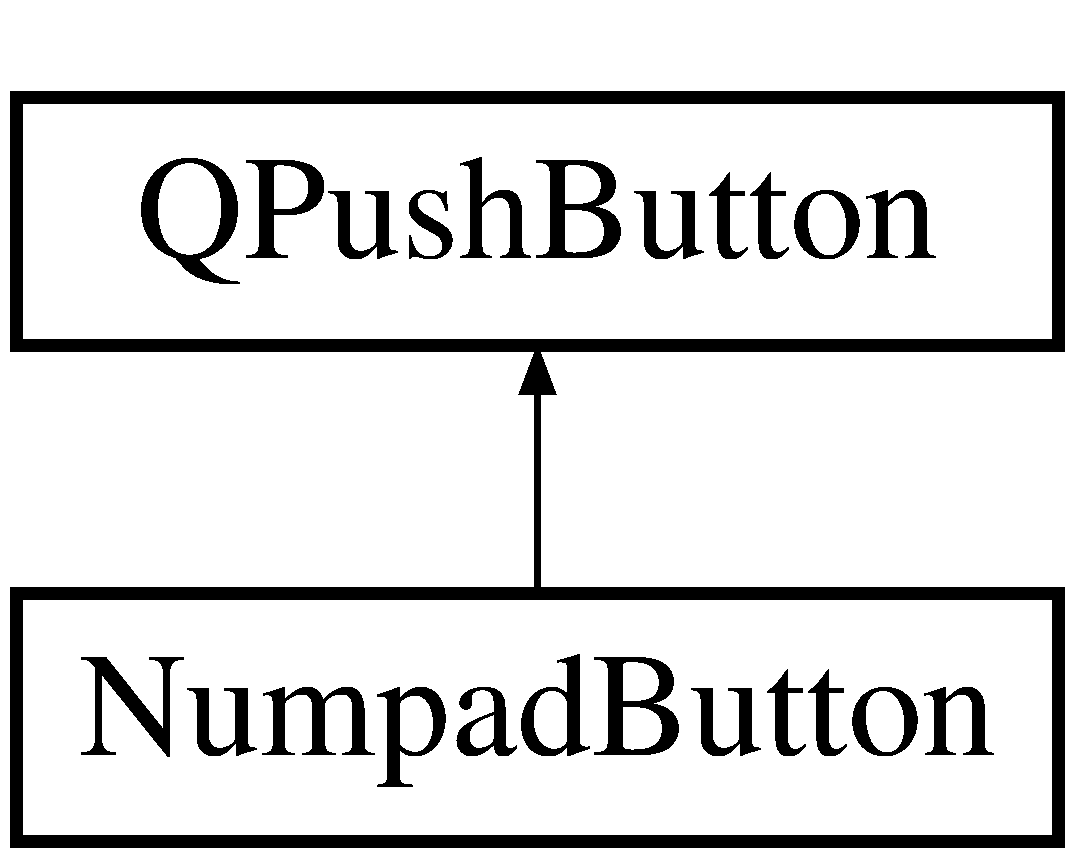
\includegraphics[height=2.000000cm]{classNumpadButton}
\end{center}
\end{figure}
\subsubsection*{Signals}
\begin{DoxyCompactItemize}
\item 
void \mbox{\hyperlink{classNumpadButton_abb1a48f3c07d93edef33528e70e77ed7}{clicked}} (int \mbox{\hyperlink{classNumpadButton_a30f48faa378ce82a0cf63f6cdd781f0b}{index}})
\end{DoxyCompactItemize}
\subsubsection*{Public Member Functions}
\begin{DoxyCompactItemize}
\item 
\mbox{\hyperlink{classNumpadButton_af9f2a23d3636ab52dc1a9fd3b08d7275}{Numpad\+Button}} (unsigned int input\+Number, Q\+String name)
\end{DoxyCompactItemize}
\subsubsection*{Private Slots}
\begin{DoxyCompactItemize}
\item 
void \mbox{\hyperlink{classNumpadButton_ae8d4b24f9b83f0cb9cc9a97c0e1055e4}{this\+Clicked}} ()
\end{DoxyCompactItemize}
\subsubsection*{Private Attributes}
\begin{DoxyCompactItemize}
\item 
unsigned int \mbox{\hyperlink{classNumpadButton_a30f48faa378ce82a0cf63f6cdd781f0b}{index}}
\end{DoxyCompactItemize}


\subsubsection{Constructor \& Destructor Documentation}
\mbox{\Hypertarget{classNumpadButton_af9f2a23d3636ab52dc1a9fd3b08d7275}\label{classNumpadButton_af9f2a23d3636ab52dc1a9fd3b08d7275}} 
\index{Numpad\+Button@{Numpad\+Button}!Numpad\+Button@{Numpad\+Button}}
\index{Numpad\+Button@{Numpad\+Button}!Numpad\+Button@{Numpad\+Button}}
{\footnotesize\ttfamily Numpad\+Button\+::\texorpdfstring{Numpad\+Button}{NumpadButton} (\begin{DoxyParamCaption}\item[{unsigned int}]{input\+Number,  }\item[{Q\+String}]{name }\end{DoxyParamCaption})} - reimplemented constructor of Q\+Push\+Button class. Initialize button and set value of \hyperlink{classNumpadButton_a30f48faa378ce82a0cf63f6cdd781f0b}{index} with given parameter. Connect standard Q\+Push\+Button::clicked() signal to \hyperlink{classNumpadButton_ae8d4b24f9b83f0cb9cc9a97c0e1055e4}{this\+Clicked}(...) function.


\subsubsection{Member Function Documentation}
\mbox{\Hypertarget{classNumpadButton_abb1a48f3c07d93edef33528e70e77ed7}\label{classNumpadButton_abb1a48f3c07d93edef33528e70e77ed7}} 
\index{Numpad\+Button@{Numpad\+Button}!clicked@{clicked}}
\index{clicked@{clicked}!Numpad\+Button@{Numpad\+Button}}
{\footnotesize\ttfamily void Numpad\+Button\+::\texorpdfstring{clicked}{clicked} (\begin{DoxyParamCaption}\item[{int}]{index }\end{DoxyParamCaption})\hspace{0.3cm}{\ttfamily [signal]}} - signal which emitted when button is  clicked with \hyperlink{classNumpadButton_ae8d4b24f9b83f0cb9cc9a97c0e1055e4}{this\+Clicked}(...) function. Signal transmit value of \hyperlink{classNumpadButton_a30f48faa378ce82a0cf63f6cdd781f0b}{index} variable in parameters. Signal handle in parent object.

\mbox{\Hypertarget{classNumpadButton_ae8d4b24f9b83f0cb9cc9a97c0e1055e4}\label{classNumpadButton_ae8d4b24f9b83f0cb9cc9a97c0e1055e4}} 
\index{Numpad\+Button@{Numpad\+Button}!this\+Clicked@{this\+Clicked}}
\index{this\+Clicked@{this\+Clicked}!Numpad\+Button@{Numpad\+Button}}
{\footnotesize\ttfamily void Numpad\+Button\+::\texorpdfstring{this\+Clicked}{thisClicked} (\begin{DoxyParamCaption}{ }\end{DoxyParamCaption})\hspace{0.3cm}{\ttfamily [inline]}, {\ttfamily [private]}, {\ttfamily [slot]}} - function called by Q\+Push\+Button::clicked() signal and emit \hyperlink{classNumpadButton_abb1a48f3c07d93edef33528e70e77ed7}{clicked}(...) signal.

\subsubsection{Member Data Documentation}
\mbox{\Hypertarget{classNumpadButton_a30f48faa378ce82a0cf63f6cdd781f0b}\label{classNumpadButton_a30f48faa378ce82a0cf63f6cdd781f0b}} 
\index{Numpad\+Button@{Numpad\+Button}!index@{index}}
\index{index@{index}!Numpad\+Button@{Numpad\+Button}}
{\footnotesize\ttfamily unsigned int Numpad\+Button\+::\texorpdfstring{index}{index}\hspace{0.3cm}{\ttfamily [private]}}

The documentation for this class was generated from the following files\+:\begin{DoxyCompactItemize}
\item 
\mbox{\hyperlink{numpaddialog_8h}{numpaddialog.\+h}}\item 
\mbox{\hyperlink{numpaddialog_8cpp}{numpaddialog.\+cpp}}\end{DoxyCompactItemize}
\newpage
\hypertarget{classNumpadDialog}{}\subsection{Numpad\+Dialog Class Reference}
\label{classNumpadDialog}\index{Numpad\+Dialog@{Numpad\+Dialog}}


{\ttfamily \#include $<$numpaddialog.\+h$>$}

Inheritance diagram for Numpad\+Dialog\+:\begin{figure}[H]
\begin{center}
\leavevmode
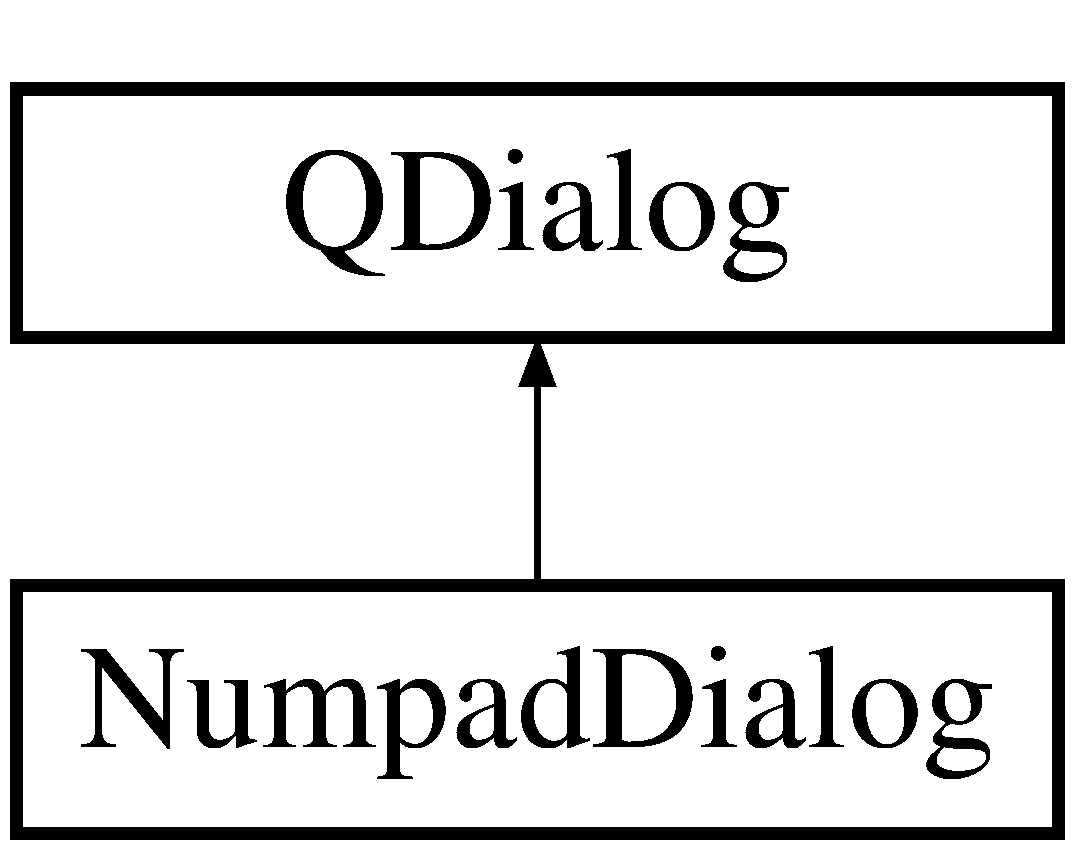
\includegraphics[height=2.000000cm]{classNumpadDialog}
\end{center}
\end{figure}
\subsubsection*{Signals}
\begin{DoxyCompactItemize}
\item 
void \mbox{\hyperlink{classNumpadDialog_ada306195f37d11153dba09bbfa35ac84}{value\+Submited}} (Q\+String \mbox{\hyperlink{classNumpadDialog_ad5046b269957f80f82d36b7ab800fc5d}{value}})
\end{DoxyCompactItemize}
\subsubsection*{Public Member Functions}
\begin{DoxyCompactItemize}
\item 
\mbox{\hyperlink{classNumpadDialog_aa6757d0d987f0be6acffbc4b64551252}{Numpad\+Dialog}} (Q\+Widget $\ast$parent=0, Q\+String window\+Title=\char`\"{}Numpad\char`\"{})
\item 
\mbox{\hyperlink{classNumpadDialog_a1aaf28df454bd5bbf2ab3829df0fcd8f}{$\sim$\+Numpad\+Dialog}} ()
\end{DoxyCompactItemize}
\subsubsection*{Static Public Member Functions}
\begin{DoxyCompactItemize}
\item 
static double \mbox{\hyperlink{classNumpadDialog_a0da4d8e9b7a4c80663421109e6bb68d0}{get\+Value}} (Q\+Widget $\ast$parent=0, Q\+String window\+Title=\char`\"{}Numpad\char`\"{})
\end{DoxyCompactItemize}
\subsubsection*{Protected Member Functions}
\begin{DoxyCompactItemize}
\item 
void \mbox{\hyperlink{classNumpadDialog_a73f71a3f983e17628468bf843643542e}{change\+Event}} (Q\+Event $\ast$event)
\end{DoxyCompactItemize}
\subsubsection*{Private Slots}
\begin{DoxyCompactItemize}
\item 
void \mbox{\hyperlink{classNumpadDialog_a717c92c0ce30150bcb0d8bb963ba4b9a}{append\+To\+Line\+Edit}} (int number)
\item 
void \mbox{\hyperlink{classNumpadDialog_a09ad5d99606896df04a2e769595d7c7c}{submit\+Value}} ()
\item 
void \mbox{\hyperlink{classNumpadDialog_a588795ce96e78c629ac1825b9f3ab21d}{change\+Sign}} ()
\item 
void \mbox{\hyperlink{classNumpadDialog_a195579dcc41869beef3b584451614013}{append\+Zero}} ()
\item 
void \mbox{\hyperlink{classNumpadDialog_aeceb302071f824e0e725867eb8be11b5}{add\+Dot}} ()
\item 
void \mbox{\hyperlink{classNumpadDialog_ac0f1db7275e66501c52a5c1b9348ebd6}{backspace}} ()
\end{DoxyCompactItemize}
\subsubsection*{Private Attributes}
\begin{DoxyCompactItemize}
\item 
Ui\+::\+Numpad\+Dialog $\ast$ \mbox{\hyperlink{classNumpadDialog_a56da5fc9be6f1c34951959598cbdd187}{ui}}
\item 
\mbox{\hyperlink{classNumpadButton}{Numpad\+Button}} $\ast$ \mbox{\hyperlink{classNumpadDialog_a3b2f37aea17608ca6040eb8efa6c4cf9}{buttons}} \mbox{[}10\mbox{]}
\item 
const Q\+String \mbox{\hyperlink{classNumpadDialog_a28b20ba1a580943985c1791dde15bcb3}{st\+Sheet}}
\item 
Q\+Action $\ast$ \mbox{\hyperlink{classNumpadDialog_ae45e9a3690fa153aa637027397db1671}{action\+Submit}}
\item 
double \mbox{\hyperlink{classNumpadDialog_ad5046b269957f80f82d36b7ab800fc5d}{value}}
\end{DoxyCompactItemize}


\subsubsection{Constructor \& Destructor Documentation}
\mbox{\Hypertarget{classNumpadDialog_aa6757d0d987f0be6acffbc4b64551252}\label{classNumpadDialog_aa6757d0d987f0be6acffbc4b64551252}} 
\index{Numpad\+Dialog@{Numpad\+Dialog}!Numpad\+Dialog@{Numpad\+Dialog}}
\index{Numpad\+Dialog@{Numpad\+Dialog}!Numpad\+Dialog@{Numpad\+Dialog}}
{\footnotesize\ttfamily Numpad\+Dialog\+::\texorpdfstring{Numpad\+Dialog}{NumpadDialog} (\begin{DoxyParamCaption}\item[{Q\+Widget $\ast$}]{parent = {\ttfamily 0},  }\item[{Q\+String}]{window\+Title = {\ttfamily \char`\"{}Numpad\char`\"{}} }\end{DoxyParamCaption})\hspace{0.3cm}{\ttfamily [explicit]}} - standard Q\+Dialog constructor.

\mbox{\Hypertarget{classNumpadDialog_a1aaf28df454bd5bbf2ab3829df0fcd8f}\label{classNumpadDialog_a1aaf28df454bd5bbf2ab3829df0fcd8f}} 
\index{Numpad\+Dialog@{Numpad\+Dialog}!````~Numpad\+Dialog@{$\sim$\+Numpad\+Dialog}}
\index{````~Numpad\+Dialog@{$\sim$\+Numpad\+Dialog}!Numpad\+Dialog@{Numpad\+Dialog}}
{\footnotesize\ttfamily Numpad\+Dialog\+::\texorpdfstring{$\sim$\+Numpad\+Dialog}{~NumpadDialog}(\begin{DoxyParamCaption}{ }\end{DoxyParamCaption})} - standard Q\+Dialog destructor. 



\subsubsection{Member Function Documentation}
\mbox{\Hypertarget{classNumpadDialog_aeceb302071f824e0e725867eb8be11b5}\label{classNumpadDialog_aeceb302071f824e0e725867eb8be11b5}} 
\index{Numpad\+Dialog@{Numpad\+Dialog}!add\+Dot@{add\+Dot}}
\index{add\+Dot@{add\+Dot}!Numpad\+Dialog@{Numpad\+Dialog}}
{\footnotesize\ttfamily void Numpad\+Dialog\+::\texorpdfstring{add\+Dot}{addDot} (\begin{DoxyParamCaption}{ }\end{DoxyParamCaption})\hspace{0.3cm}{\ttfamily [private]}, {\ttfamily [slot]}} - function to add dot to text field.

\mbox{\Hypertarget{classNumpadDialog_a717c92c0ce30150bcb0d8bb963ba4b9a}\label{classNumpadDialog_a717c92c0ce30150bcb0d8bb963ba4b9a}} 
\index{Numpad\+Dialog@{Numpad\+Dialog}!append\+To\+Line\+Edit@{append\+To\+Line\+Edit}}
\index{append\+To\+Line\+Edit@{append\+To\+Line\+Edit}!Numpad\+Dialog@{Numpad\+Dialog}}
{\footnotesize\ttfamily void Numpad\+Dialog\+::\texorpdfstring{append\+To\+Line\+Edit}{appendToLineEdit} (\begin{DoxyParamCaption}\item[{int}]{number }\end{DoxyParamCaption})\hspace{0.3cm}{\ttfamily [private]}, {\ttfamily [slot]}} - function which used to add number to text field. Function called by 1..9 button from \hyperlink{classNumpadDialog_a3b2f37aea17608ca6040eb8efa6c4cf9}{buttons} array.

\mbox{\Hypertarget{classNumpadDialog_a195579dcc41869beef3b584451614013}\label{classNumpadDialog_a195579dcc41869beef3b584451614013}} 
\index{Numpad\+Dialog@{Numpad\+Dialog}!append\+Zero@{append\+Zero}}
\index{append\+Zero@{append\+Zero}!Numpad\+Dialog@{Numpad\+Dialog}}
{\footnotesize\ttfamily void Numpad\+Dialog\+::\texorpdfstring{append\+Zero}{appendZero} (\begin{DoxyParamCaption}{ }\end{DoxyParamCaption})\hspace{0.3cm}{\ttfamily [private]}, {\ttfamily [slot]}} - function which used to add zero to text field. Function called by 0 button from \hyperlink{classNumpadDialog_a3b2f37aea17608ca6040eb8efa6c4cf9}{buttons} array.

\mbox{\Hypertarget{classNumpadDialog_ac0f1db7275e66501c52a5c1b9348ebd6}\label{classNumpadDialog_ac0f1db7275e66501c52a5c1b9348ebd6}} 
\index{Numpad\+Dialog@{Numpad\+Dialog}!backspace@{backspace}}
\index{backspace@{backspace}!Numpad\+Dialog@{Numpad\+Dialog}}
{\footnotesize\ttfamily void Numpad\+Dialog\+::\texorpdfstring{backspace}{backspace} (\begin{DoxyParamCaption}{ }\end{DoxyParamCaption})\hspace{0.3cm}{\ttfamily [private]}, {\ttfamily [slot]}} - function to remove last symbol from text field.

\mbox{\Hypertarget{classNumpadDialog_a73f71a3f983e17628468bf843643542e}\label{classNumpadDialog_a73f71a3f983e17628468bf843643542e}} 
\index{Numpad\+Dialog@{Numpad\+Dialog}!change\+Event@{change\+Event}}
\index{change\+Event@{change\+Event}!Numpad\+Dialog@{Numpad\+Dialog}}
{\footnotesize\ttfamily void Numpad\+Dialog\+::\texorpdfstring{change\+Event}{changeEvent} (\begin{DoxyParamCaption}\item[{Q\+Event $\ast$}]{event }\end{DoxyParamCaption})\hspace{0.3cm}{\ttfamily [protected]}} - reimplementation of default event of Q\+Widget to enable user interface translation. Function called automatically.

\mbox{\Hypertarget{classNumpadDialog_a588795ce96e78c629ac1825b9f3ab21d}\label{classNumpadDialog_a588795ce96e78c629ac1825b9f3ab21d}} 
\index{Numpad\+Dialog@{Numpad\+Dialog}!change\+Sign@{change\+Sign}}
\index{change\+Sign@{change\+Sign}!Numpad\+Dialog@{Numpad\+Dialog}}
{\footnotesize\ttfamily void Numpad\+Dialog\+::\texorpdfstring{change\+Sign}{changeSign} (\begin{DoxyParamCaption}{ }\end{DoxyParamCaption})\hspace{0.3cm}{\ttfamily [private]}, {\ttfamily [slot]}} - function to change sign of number which is st text field. 

\mbox{\Hypertarget{classNumpadDialog_a0da4d8e9b7a4c80663421109e6bb68d0}\label{classNumpadDialog_a0da4d8e9b7a4c80663421109e6bb68d0}} 
\index{Numpad\+Dialog@{Numpad\+Dialog}!get\+Value@{get\+Value}}
\index{get\+Value@{get\+Value}!Numpad\+Dialog@{Numpad\+Dialog}}
{\footnotesize\ttfamily double Numpad\+Dialog\+::\texorpdfstring{get\+Value}{getValue} (\begin{DoxyParamCaption}\item[{Q\+Widget $\ast$}]{parent = {\ttfamily 0},  }\item[{Q\+String}]{window\+Title = {\ttfamily \char`\"{}Numpad\char`\"{}} }\end{DoxyParamCaption})\hspace{0.3cm}{\ttfamily [static]}} - static function of class used to show dialog and get \textit{double} value.

\mbox{\Hypertarget{classNumpadDialog_a09ad5d99606896df04a2e769595d7c7c}\label{classNumpadDialog_a09ad5d99606896df04a2e769595d7c7c}} 
\index{Numpad\+Dialog@{Numpad\+Dialog}!submit\+Value@{submit\+Value}}
\index{submit\+Value@{submit\+Value}!Numpad\+Dialog@{Numpad\+Dialog}}
{\footnotesize\ttfamily void Numpad\+Dialog\+::\texorpdfstring{submit\+Value}{submitValue} (\begin{DoxyParamCaption}{ }\end{DoxyParamCaption})\hspace{0.3cm}{\ttfamily [private]}, {\ttfamily [slot]}} - function to transform text at text field to \textit{double} number and put it to \hyperlink{classNumpadDialog_ad5046b269957f80f82d36b7ab800fc5d}{value} variable.

\mbox{\Hypertarget{classNumpadDialog_ada306195f37d11153dba09bbfa35ac84}\label{classNumpadDialog_ada306195f37d11153dba09bbfa35ac84}} 
\index{Numpad\+Dialog@{Numpad\+Dialog}!value\+Submited@{value\+Submited}}
\index{value\+Submited@{value\+Submited}!Numpad\+Dialog@{Numpad\+Dialog}}
{\footnotesize\ttfamily void Numpad\+Dialog\+::\texorpdfstring{value\+Submited}{valueSubmited} (\begin{DoxyParamCaption}\item[{Q\+String}]{value }\end{DoxyParamCaption})\hspace{0.3cm}{\ttfamily [signal]}} - unused.



\subsubsection{Member Data Documentation}
\mbox{\Hypertarget{classNumpadDialog_ae45e9a3690fa153aa637027397db1671}\label{classNumpadDialog_ae45e9a3690fa153aa637027397db1671}} 
\index{Numpad\+Dialog@{Numpad\+Dialog}!action\+Submit@{action\+Submit}}
\index{action\+Submit@{action\+Submit}!Numpad\+Dialog@{Numpad\+Dialog}}
{\footnotesize\ttfamily Q\+Action$\ast$ Numpad\+Dialog\+::\texorpdfstring{action\+Submit}{actionSubmit}\hspace{0.3cm}{\ttfamily [private]}}

\mbox{\Hypertarget{classNumpadDialog_a3b2f37aea17608ca6040eb8efa6c4cf9}\label{classNumpadDialog_a3b2f37aea17608ca6040eb8efa6c4cf9}} 
\index{Numpad\+Dialog@{Numpad\+Dialog}!buttons@{buttons}}
\index{buttons@{buttons}!Numpad\+Dialog@{Numpad\+Dialog}}
{\footnotesize\ttfamily \mbox{\hyperlink{classNumpadButton}{Numpad\+Button}}$\ast$ Numpad\+Dialog\+::\texorpdfstring{buttons}{buttons}\mbox{[}10\mbox{]}\hspace{0.3cm}{\ttfamily [private]}}

\mbox{\Hypertarget{classNumpadDialog_a28b20ba1a580943985c1791dde15bcb3}\label{classNumpadDialog_a28b20ba1a580943985c1791dde15bcb3}} 
\index{Numpad\+Dialog@{Numpad\+Dialog}!st\+Sheet@{st\+Sheet}}
\index{st\+Sheet@{st\+Sheet}!Numpad\+Dialog@{Numpad\+Dialog}}
{\footnotesize\ttfamily const Q\+String Numpad\+Dialog\+::\texorpdfstring{st\+Sheet}{stSheet}\hspace{0.3cm}{\ttfamily [private]}}

\mbox{\Hypertarget{classNumpadDialog_ad5046b269957f80f82d36b7ab800fc5d}\label{classNumpadDialog_ad5046b269957f80f82d36b7ab800fc5d}} 
\index{Numpad\+Dialog@{Numpad\+Dialog}!value@{value}}
\index{value@{value}!Numpad\+Dialog@{Numpad\+Dialog}}
{\footnotesize\ttfamily double Numpad\+Dialog\+::\texorpdfstring{value}{value}\hspace{0.3cm}{\ttfamily [private]}}



The documentation for this class was generated from the following files\+:\begin{DoxyCompactItemize}
\item 
\mbox{\hyperlink{numpaddialog_8h}{numpaddialog.\+h}}\item 
\mbox{\hyperlink{numpaddialog_8cpp}{numpaddialog.\+cpp}}\end{DoxyCompactItemize}
\newpage
\hypertarget{structRegister_1_1MasterReg___1_1reg}{}\subsection{Register\+:\+:Master\+Reg\+\_\+\+:\+:reg Struct Reference}
\label{structRegister_1_1MasterReg___1_1reg}\index{Register\+::\+Master\+Reg\+\_\+\+::reg@{Register\+::\+Master\+Reg\+\_\+\+::reg}}


{\ttfamily \#include $<$settings.\+h$>$}

Fields of structure describe data places at master board to setup machine states and parameters.

\subsubsection*{Public Attributes}
\begin{DoxyCompactItemize}
\item 
\mbox{\hyperlink{settings_8h_a017dd44e68049ffdd31500a8cd01ba68}{uint16\+\_\+t}} \mbox{\hyperlink{structRegister_1_1MasterReg___1_1reg_a4fef9fe3c083d9d8ea2edc13ca46dd2d}{master\+Reg\+\_\+\+D\+E\+V\+\_\+\+I\+N\+F\+\_\+H}}
\item 
\mbox{\hyperlink{settings_8h_a017dd44e68049ffdd31500a8cd01ba68}{uint16\+\_\+t}} \mbox{\hyperlink{structRegister_1_1MasterReg___1_1reg_aceefceadc269f1d7b7d1bca7d5071025}{master\+Reg\+\_\+\+S\+I\+ZE}}
\item 
\mbox{\hyperlink{settings_8h_a017dd44e68049ffdd31500a8cd01ba68}{uint16\+\_\+t}} \mbox{\hyperlink{structRegister_1_1MasterReg___1_1reg_a06032ddd4d9b8205192c2828937cb51d}{\+\_\+res}}
\item 
\mbox{\hyperlink{settings_8h_a017dd44e68049ffdd31500a8cd01ba68}{uint16\+\_\+t}} \mbox{\hyperlink{structRegister_1_1MasterReg___1_1reg_a540444f341997eeb2dfa619a4a193d61}{master\+Reg\+\_\+\+P\+RZ}}
\item 
\mbox{\hyperlink{settings_8h_a017dd44e68049ffdd31500a8cd01ba68}{uint16\+\_\+t}} \mbox{\hyperlink{structRegister_1_1MasterReg___1_1reg_a4e2d6361583dd5aebbfbf108e851db7c}{master\+Reg\+\_\+\+S\+TA}}
\item 
\mbox{\hyperlink{settings_8h_a017dd44e68049ffdd31500a8cd01ba68}{uint16\+\_\+t}} \mbox{\hyperlink{structRegister_1_1MasterReg___1_1reg_a42c97dcb18a310e8d484dd2d9edc577d}{masterhead\+Reg}}
\item 
\mbox{\hyperlink{settings_8h_a017dd44e68049ffdd31500a8cd01ba68}{uint16\+\_\+t}} \mbox{\hyperlink{structRegister_1_1MasterReg___1_1reg_acec853c8a9191208a9629aa9702c1931}{master\+Reg\+\_\+\+L\+AM}}
\item 
\mbox{\hyperlink{settings_8h_a017dd44e68049ffdd31500a8cd01ba68}{uint16\+\_\+t}} \mbox{\hyperlink{structRegister_1_1MasterReg___1_1reg_a4078de112432b3218faa19e8c7b764ae}{master\+Reg\+\_\+\+T\+O\+T\+A\+LH}}
\item 
\mbox{\hyperlink{settings_8h_a017dd44e68049ffdd31500a8cd01ba68}{uint16\+\_\+t}} \mbox{\hyperlink{structRegister_1_1MasterReg___1_1reg_ac232feff140996bd7b79900063ffd4e5}{master\+Reg\+\_\+\+T\+O\+T\+A\+LL}}
\item 
\mbox{\hyperlink{settings_8h_a017dd44e68049ffdd31500a8cd01ba68}{uint16\+\_\+t}} \mbox{\hyperlink{structRegister_1_1MasterReg___1_1reg_a4d87d02520b9b786d6474a563b03bfda}{masterhead\+Reg1}}
\item 
\mbox{\hyperlink{settings_8h_a017dd44e68049ffdd31500a8cd01ba68}{uint16\+\_\+t}} \mbox{\hyperlink{structRegister_1_1MasterReg___1_1reg_a9e97c3a0d77f6e3e2cac930ec361249c}{master\+Reg\+\_\+\+P\+AL}}
\item 
\mbox{\hyperlink{settings_8h_a017dd44e68049ffdd31500a8cd01ba68}{uint16\+\_\+t}} \mbox{\hyperlink{structRegister_1_1MasterReg___1_1reg_a9e5f8080f842031b2711e280139e2275}{master\+Reg\+\_\+\+I\+N\+P\+UT}}
\item 
\mbox{\hyperlink{settings_8h_a017dd44e68049ffdd31500a8cd01ba68}{uint16\+\_\+t}} \mbox{\hyperlink{structRegister_1_1MasterReg___1_1reg_a56a643e4e412e720f3aeba691f136cd1}{master\+Reg\+\_\+\+R\+E\+M\+A\+I\+NH}}
\item 
\mbox{\hyperlink{settings_8h_a017dd44e68049ffdd31500a8cd01ba68}{uint16\+\_\+t}} \mbox{\hyperlink{structRegister_1_1MasterReg___1_1reg_ac9feb63734161b0f3f2b662b44be2a60}{master\+Reg\+\_\+\+R\+E\+M\+A\+I\+NL}}
\item 
\mbox{\hyperlink{settings_8h_a017dd44e68049ffdd31500a8cd01ba68}{uint16\+\_\+t}} \mbox{\hyperlink{structRegister_1_1MasterReg___1_1reg_ae2bc8af479ef3de52ea21d93678381b9}{master\+Reg\+\_\+\+S\+P\+E\+ED}}
\item 
\mbox{\hyperlink{settings_8h_a017dd44e68049ffdd31500a8cd01ba68}{uint16\+\_\+t}} \mbox{\hyperlink{structRegister_1_1MasterReg___1_1reg_aa884aabc402a552b82d06b7b32b5546b}{master\+Reg\+\_\+\+P\+R\+I\+N\+T\+E\+DH}}
\item 
\mbox{\hyperlink{settings_8h_a017dd44e68049ffdd31500a8cd01ba68}{uint16\+\_\+t}} \mbox{\hyperlink{structRegister_1_1MasterReg___1_1reg_a59c35ffa9740d665882807b5f6e94ddc}{master\+Reg\+\_\+\+P\+R\+I\+N\+T\+E\+DL}}
\item 
\mbox{\hyperlink{settings_8h_a017dd44e68049ffdd31500a8cd01ba68}{uint16\+\_\+t}} \mbox{\hyperlink{structRegister_1_1MasterReg___1_1reg_a44633bb0942fe0614b9bea8d5645596f}{master\+Reg\+\_\+\+M\+A\+C\+H\+I\+N\+E\+\_\+\+T\+Y\+PE}}
\item 
\mbox{\hyperlink{settings_8h_a017dd44e68049ffdd31500a8cd01ba68}{uint16\+\_\+t}} \mbox{\hyperlink{structRegister_1_1MasterReg___1_1reg_a14b51bf5fde2859d4750d525c7e21d55}{master\+Reg\+\_\+\+P\+A\+L1}}
\item 
\mbox{\hyperlink{settings_8h_a017dd44e68049ffdd31500a8cd01ba68}{uint16\+\_\+t}} \mbox{\hyperlink{structRegister_1_1MasterReg___1_1reg_aa5111a7f8eddbd8f8d6c92e23f326946}{master\+Reg\+\_\+\+E\+KR}}
\item 
\mbox{\hyperlink{settings_8h_a017dd44e68049ffdd31500a8cd01ba68}{uint16\+\_\+t}} \mbox{\hyperlink{structRegister_1_1MasterReg___1_1reg_a50488597048779e728398256d6d0abb6}{master\+Reg\+\_\+\+A\+C\+T\+I\+V\+H\+E\+A\+D\+\_\+L}}
\item 
\mbox{\hyperlink{settings_8h_a017dd44e68049ffdd31500a8cd01ba68}{uint16\+\_\+t}} \mbox{\hyperlink{structRegister_1_1MasterReg___1_1reg_aba9351ca12403b7e4d4614f028b546b6}{master\+Reg\+\_\+\+A\+C\+T\+I\+V\+H\+E\+A\+D\+\_\+H}}
\item 
\mbox{\hyperlink{settings_8h_a017dd44e68049ffdd31500a8cd01ba68}{uint16\+\_\+t}} \mbox{\hyperlink{structRegister_1_1MasterReg___1_1reg_ac9881986892437a22eb3fe27ce8136c8}{master\+Reg\+\_\+\+D\+E\+V\+E\+RR}}
\item 
\mbox{\hyperlink{settings_8h_a017dd44e68049ffdd31500a8cd01ba68}{uint16\+\_\+t}} \mbox{\hyperlink{structRegister_1_1MasterReg___1_1reg_a7be5288f63c9e6abe8970516b7ad8544}{master\+Reg\+\_\+\+E\+RR}}
\item 
\mbox{\hyperlink{settings_8h_a017dd44e68049ffdd31500a8cd01ba68}{uint16\+\_\+t}} \mbox{\hyperlink{structRegister_1_1MasterReg___1_1reg_a8b8b9ba47acd91fb4ddfa4eeeafced19}{master\+Reg\+\_\+\+K\+O\+DH}}
\item 
\mbox{\hyperlink{settings_8h_a017dd44e68049ffdd31500a8cd01ba68}{uint16\+\_\+t}} \mbox{\hyperlink{structRegister_1_1MasterReg___1_1reg_a20e6b823b310dbea2e911de314b38f49}{master\+Reg\+\_\+\+K\+O\+DL}}
\item 
\mbox{\hyperlink{settings_8h_a017dd44e68049ffdd31500a8cd01ba68}{uint16\+\_\+t}} \mbox{\hyperlink{structRegister_1_1MasterReg___1_1reg_af5029f6053b7b8dab2d3aebe1c0649dd}{master\+Reg\+\_\+\+D\+A\+TH}}
\item 
\mbox{\hyperlink{settings_8h_a017dd44e68049ffdd31500a8cd01ba68}{uint16\+\_\+t}} \mbox{\hyperlink{structRegister_1_1MasterReg___1_1reg_a630bf9078970e9ac972b240c8117056c}{master\+Reg\+\_\+\+D\+A\+TL}}
\item 
\mbox{\hyperlink{settings_8h_a017dd44e68049ffdd31500a8cd01ba68}{uint16\+\_\+t}} \mbox{\hyperlink{structRegister_1_1MasterReg___1_1reg_a66220c08a03513ed70faac3e9d352a0e}{master\+Reg\+\_\+\+K\+O\+D\+\_\+\+ON}}
\item 
\mbox{\hyperlink{settings_8h_a017dd44e68049ffdd31500a8cd01ba68}{uint16\+\_\+t}} \mbox{\hyperlink{structRegister_1_1MasterReg___1_1reg_a7e102b082ae10861d4430c46acd12307}{master\+Reg\+\_\+\+D\+AT}}
\item 
\mbox{\hyperlink{settings_8h_a017dd44e68049ffdd31500a8cd01ba68}{uint16\+\_\+t}} \mbox{\hyperlink{structRegister_1_1MasterReg___1_1reg_a3a4832587b7dda4714322b2a4ed464c2}{R\+E\+G\+\_\+\+K\+O\+D\+\_\+\+W\+P\+I\+SZ}}
\item 
\mbox{\hyperlink{settings_8h_a017dd44e68049ffdd31500a8cd01ba68}{uint16\+\_\+t}} \mbox{\hyperlink{structRegister_1_1MasterReg___1_1reg_a357c11013ba334079a88bc9c49b6cb3d}{master\+Reg\+\_\+\+H\+RW}}
\item 
\mbox{\hyperlink{settings_8h_a017dd44e68049ffdd31500a8cd01ba68}{uint16\+\_\+t}} \mbox{\hyperlink{structRegister_1_1MasterReg___1_1reg_a476ef908b88923095d4854dcffa3e449}{master\+Reg\+\_\+\+H\+R\+W1}}
\item 
\mbox{\hyperlink{settings_8h_a017dd44e68049ffdd31500a8cd01ba68}{uint16\+\_\+t}} \mbox{\hyperlink{structRegister_1_1MasterReg___1_1reg_a81eeb4dd03eaf29676703e60f6dd5647}{master\+Reg\+\_\+\+K\+O\+D\+\_\+\+O\+N2}}
\item 
\mbox{\hyperlink{settings_8h_a017dd44e68049ffdd31500a8cd01ba68}{uint16\+\_\+t}} \mbox{\hyperlink{structRegister_1_1MasterReg___1_1reg_a9ba85903b95886b7a305553b8757f1f6}{master\+Reg\+\_\+\+K\+O\+D\+\_\+\+O\+N3}}
\item 
\mbox{\hyperlink{settings_8h_a017dd44e68049ffdd31500a8cd01ba68}{uint16\+\_\+t}} \mbox{\hyperlink{structRegister_1_1MasterReg___1_1reg_adda765befe3afc716d8ef69909ec92be}{master\+Reg\+\_\+\+E\+R\+R\+O\+R\+\_\+\+M\+E\+S\+S\+A\+GE}}
\item 
\mbox{\hyperlink{settings_8h_a017dd44e68049ffdd31500a8cd01ba68}{uint16\+\_\+t}} \mbox{\hyperlink{structRegister_1_1MasterReg___1_1reg_a253168290103d94eac25407b082deaae}{master\+Reg\+\_\+\+D\+E\+V\+\_\+\+I\+N\+F\+\_\+L}}
\end{DoxyCompactItemize}


\subsubsection{Member Data Documentation}
\mbox{\Hypertarget{structRegister_1_1MasterReg___1_1reg_a06032ddd4d9b8205192c2828937cb51d}\label{structRegister_1_1MasterReg___1_1reg_a06032ddd4d9b8205192c2828937cb51d}} 
\index{Register\+::\+Master\+Reg\+\_\+\+::reg@{Register\+::\+Master\+Reg\+\_\+\+::reg}!\+\_\+res@{\+\_\+res}}
\index{\+\_\+res@{\+\_\+res}!Register\+::\+Master\+Reg\+\_\+\+::reg@{Register\+::\+Master\+Reg\+\_\+\+::reg}}
{\footnotesize\ttfamily \mbox{\hyperlink{settings_8h_a017dd44e68049ffdd31500a8cd01ba68}{uint16\+\_\+t}} Register\+::\+Master\+Reg\+\_\+\+::\texorpdfstring{\+\_\+res}{\_res}} - reserved field.

\mbox{\Hypertarget{structRegister_1_1MasterReg___1_1reg_a42c97dcb18a310e8d484dd2d9edc577d}\label{structRegister_1_1MasterReg___1_1reg_a42c97dcb18a310e8d484dd2d9edc577d}} 
\index{Register\+::\+Master\+Reg\+\_\+\+::reg@{Register\+::\+Master\+Reg\+\_\+\+::reg}!masterhead\+Reg@{masterhead\+Reg}}
\index{masterhead\+Reg@{masterhead\+Reg}!Register\+::\+Master\+Reg\+\_\+\+::reg@{Register\+::\+Master\+Reg\+\_\+\+::reg}}
{\footnotesize\ttfamily \mbox{\hyperlink{settings_8h_a017dd44e68049ffdd31500a8cd01ba68}{uint16\+\_\+t}} Register\+::\+Master\+Reg\+\_\+\+::reg\+::\texorpdfstring{masterhead\+Reg}{masterheadReg}} - States of the Heads On/Off buttons. Low Word of Double Word Register

\mbox{\Hypertarget{structRegister_1_1MasterReg___1_1reg_a4d87d02520b9b786d6474a563b03bfda}\label{structRegister_1_1MasterReg___1_1reg_a4d87d02520b9b786d6474a563b03bfda}} 
\index{Register\+::\+Master\+Reg\+\_\+\+::reg@{Register\+::\+Master\+Reg\+\_\+\+::reg}!masterhead\+Reg1@{masterhead\+Reg1}}
\index{masterhead\+Reg1@{masterhead\+Reg1}!Register\+::\+Master\+Reg\+\_\+\+::reg@{Register\+::\+Master\+Reg\+\_\+\+::reg}}
{\footnotesize\ttfamily \mbox{\hyperlink{settings_8h_a017dd44e68049ffdd31500a8cd01ba68}{uint16\+\_\+t}} Register\+::\+Master\+Reg\+\_\+\+::reg\+::\texorpdfstring{masterhead\+Reg1}{masterheadReg1}} - States of the Head On/Off buttons. High Word of Double Word Register

\mbox{\Hypertarget{structRegister_1_1MasterReg___1_1reg_aba9351ca12403b7e4d4614f028b546b6}\label{structRegister_1_1MasterReg___1_1reg_aba9351ca12403b7e4d4614f028b546b6}} 
\index{Register\+::\+Master\+Reg\+\_\+\+::reg@{Register\+::\+Master\+Reg\+\_\+\+::reg}!master\+Reg\+\_\+\+A\+C\+T\+I\+V\+H\+E\+A\+D\+\_\+H@{master\+Reg\+\_\+\+A\+C\+T\+I\+V\+H\+E\+A\+D\+\_\+H}}
\index{master\+Reg\+\_\+\+A\+C\+T\+I\+V\+H\+E\+A\+D\+\_\+H@{master\+Reg\+\_\+\+A\+C\+T\+I\+V\+H\+E\+A\+D\+\_\+H}!Register\+::\+Master\+Reg\+\_\+\+::reg@{Register\+::\+Master\+Reg\+\_\+\+::reg}}
{\footnotesize\ttfamily \mbox{\hyperlink{settings_8h_a017dd44e68049ffdd31500a8cd01ba68}{uint16\+\_\+t}} Register\+::\+Master\+Reg\+\_\+\+::reg\+::\texorpdfstring{master\+Reg\+\_\+\+A\+C\+T\+I\+V\+H\+E\+A\+D\+\_\+H}{masterReg\_ACTIVHEAD\_H}} - States of the Head Activation buttons. 0 means Head is Active, 1 means Head is Not Active. High Word of Double Word Register

\mbox{\Hypertarget{structRegister_1_1MasterReg___1_1reg_a50488597048779e728398256d6d0abb6}\label{structRegister_1_1MasterReg___1_1reg_a50488597048779e728398256d6d0abb6}} 
\index{Register\+::\+Master\+Reg\+\_\+\+::reg@{Register\+::\+Master\+Reg\+\_\+\+::reg}!master\+Reg\+\_\+\+A\+C\+T\+I\+V\+H\+E\+A\+D\+\_\+L@{master\+Reg\+\_\+\+A\+C\+T\+I\+V\+H\+E\+A\+D\+\_\+L}}
\index{master\+Reg\+\_\+\+A\+C\+T\+I\+V\+H\+E\+A\+D\+\_\+L@{master\+Reg\+\_\+\+A\+C\+T\+I\+V\+H\+E\+A\+D\+\_\+L}!Register\+::\+Master\+Reg\+\_\+\+::reg@{Register\+::\+Master\+Reg\+\_\+\+::reg}}
{\footnotesize\ttfamily \mbox{\hyperlink{settings_8h_a017dd44e68049ffdd31500a8cd01ba68}{uint16\+\_\+t}} Register\+::\+Master\+Reg\+\_\+\+::reg\+::\texorpdfstring{master\+Reg\+\_\+\+A\+C\+T\+I\+V\+H\+E\+A\+D\+\_\+L}{masterReg\_ACTIVHEAD\_L}} - States of the Head Activation buttons. 0 means Head is Active, 1 means Head is Not Active. Low Word of Double Word Register

\mbox{\Hypertarget{structRegister_1_1MasterReg___1_1reg_a7e102b082ae10861d4430c46acd12307}\label{structRegister_1_1MasterReg___1_1reg_a7e102b082ae10861d4430c46acd12307}} 
\index{Register\+::\+Master\+Reg\+\_\+\+::reg@{Register\+::\+Master\+Reg\+\_\+\+::reg}!master\+Reg\+\_\+\+D\+AT@{master\+Reg\+\_\+\+D\+AT}}
\index{master\+Reg\+\_\+\+D\+AT@{master\+Reg\+\_\+\+D\+AT}!Register\+::\+Master\+Reg\+\_\+\+::reg@{Register\+::\+Master\+Reg\+\_\+\+::reg}}
{\footnotesize\ttfamily \mbox{\hyperlink{settings_8h_a017dd44e68049ffdd31500a8cd01ba68}{uint16\+\_\+t}} Register\+::\+Master\+Reg\+\_\+\+::reg\+::\texorpdfstring{master\+Reg\+\_\+\+D\+AT}{masterReg\_DAT}} - Actual Date readed from system

\mbox{\Hypertarget{structRegister_1_1MasterReg___1_1reg_af5029f6053b7b8dab2d3aebe1c0649dd}\label{structRegister_1_1MasterReg___1_1reg_af5029f6053b7b8dab2d3aebe1c0649dd}} 
\index{Register\+::\+Master\+Reg\+\_\+\+::reg@{Register\+::\+Master\+Reg\+\_\+\+::reg}!master\+Reg\+\_\+\+D\+A\+TH@{master\+Reg\+\_\+\+D\+A\+TH}}
\index{master\+Reg\+\_\+\+D\+A\+TH@{master\+Reg\+\_\+\+D\+A\+TH}!Register\+::\+Master\+Reg\+\_\+\+::reg@{Register\+::\+Master\+Reg\+\_\+\+::reg}}
{\footnotesize\ttfamily \mbox{\hyperlink{settings_8h_a017dd44e68049ffdd31500a8cd01ba68}{uint16\+\_\+t}} Register\+::\+Master\+Reg\+\_\+\+::reg\+::\texorpdfstring{master\+Reg\+\_\+\+D\+A\+TH}{masterReg\_DATH}} - Date of the installment code activation. High Word of Double Word Register

\mbox{\Hypertarget{structRegister_1_1MasterReg___1_1reg_a630bf9078970e9ac972b240c8117056c}\label{structRegister_1_1MasterReg___1_1reg_a630bf9078970e9ac972b240c8117056c}} 
\index{Register\+::\+Master\+Reg\+\_\+\+::reg@{Register\+::\+Master\+Reg\+\_\+\+::reg}!master\+Reg\+\_\+\+D\+A\+TL@{master\+Reg\+\_\+\+D\+A\+TL}}
\index{master\+Reg\+\_\+\+D\+A\+TL@{master\+Reg\+\_\+\+D\+A\+TL}!Register\+::\+Master\+Reg\+\_\+\+::reg@{Register\+::\+Master\+Reg\+\_\+\+::reg}}
{\footnotesize\ttfamily \mbox{\hyperlink{settings_8h_a017dd44e68049ffdd31500a8cd01ba68}{uint16\+\_\+t}} Register\+::\+Master\+Reg\+\_\+\+::reg\+::\texorpdfstring{master\+Reg\+\_\+\+D\+A\+TL}{masterReg\_DATL}} - Date of the installment code activation. Low Word of Double Word Register

\mbox{\Hypertarget{structRegister_1_1MasterReg___1_1reg_a4fef9fe3c083d9d8ea2edc13ca46dd2d}\label{structRegister_1_1MasterReg___1_1reg_a4fef9fe3c083d9d8ea2edc13ca46dd2d}} 
\index{Register\+::\+Master\+Reg\+\_\+\+::reg@{Register\+::\+Master\+Reg\+\_\+\+::reg}!master\+Reg\+\_\+\+D\+E\+V\+\_\+\+I\+N\+F\+\_\+H@{master\+Reg\+\_\+\+D\+E\+V\+\_\+\+I\+N\+F\+\_\+H}}
\index{master\+Reg\+\_\+\+D\+E\+V\+\_\+\+I\+N\+F\+\_\+H@{master\+Reg\+\_\+\+D\+E\+V\+\_\+\+I\+N\+F\+\_\+H}!Register\+::\+Master\+Reg\+\_\+\+::reg@{Register\+::\+Master\+Reg\+\_\+\+::reg}}
{\footnotesize\ttfamily \mbox{\hyperlink{settings_8h_a017dd44e68049ffdd31500a8cd01ba68}{uint16\+\_\+t}} Register\+::\+Master\+Reg\+\_\+\+::reg\+::\texorpdfstring{master\+Reg\+\_\+\+D\+E\+V\+\_\+\+I\+N\+F\+\_\+H}{masterReg\_DEV\_INF\_H}} - Number of PCB and version of software of MASTER. High Word of Double Word Register

\mbox{\Hypertarget{structRegister_1_1MasterReg___1_1reg_a253168290103d94eac25407b082deaae}\label{structRegister_1_1MasterReg___1_1reg_a253168290103d94eac25407b082deaae}} 
\index{Register\+::\+Master\+Reg\+\_\+\+::reg@{Register\+::\+Master\+Reg\+\_\+\+::reg}!master\+Reg\+\_\+\+D\+E\+V\+\_\+\+I\+N\+F\+\_\+L@{master\+Reg\+\_\+\+D\+E\+V\+\_\+\+I\+N\+F\+\_\+L}}
\index{master\+Reg\+\_\+\+D\+E\+V\+\_\+\+I\+N\+F\+\_\+L@{master\+Reg\+\_\+\+D\+E\+V\+\_\+\+I\+N\+F\+\_\+L}!Register\+::\+Master\+Reg\+\_\+\+::reg@{Register\+::\+Master\+Reg\+\_\+\+::reg}}
{\footnotesize\ttfamily \mbox{\hyperlink{settings_8h_a017dd44e68049ffdd31500a8cd01ba68}{uint16\+\_\+t}} Register\+::\+Master\+Reg\+\_\+\+::reg\+::\texorpdfstring{master\+Reg\+\_\+\+D\+E\+V\+\_\+\+I\+N\+F\+\_\+L}{masterReg\_DEV\_INF\_L}} - Number of the PCB and version of software of MASTER. Low Word of Double Word Register

\mbox{\Hypertarget{structRegister_1_1MasterReg___1_1reg_ac9881986892437a22eb3fe27ce8136c8}\label{structRegister_1_1MasterReg___1_1reg_ac9881986892437a22eb3fe27ce8136c8}} 
\index{Register\+::\+Master\+Reg\+\_\+\+::reg@{Register\+::\+Master\+Reg\+\_\+\+::reg}!master\+Reg\+\_\+\+D\+E\+V\+E\+RR@{master\+Reg\+\_\+\+D\+E\+V\+E\+RR}}
\index{master\+Reg\+\_\+\+D\+E\+V\+E\+RR@{master\+Reg\+\_\+\+D\+E\+V\+E\+RR}!Register\+::\+Master\+Reg\+\_\+\+::reg@{Register\+::\+Master\+Reg\+\_\+\+::reg}}
{\footnotesize\ttfamily \mbox{\hyperlink{settings_8h_a017dd44e68049ffdd31500a8cd01ba68}{uint16\+\_\+t}} Register\+::\+Master\+Reg\+\_\+\+::reg\+::\texorpdfstring{master\+Reg\+\_\+\+D\+E\+V\+E\+RR}{masterReg\_DEVERR}} - Address of the device with error

\mbox{\Hypertarget{structRegister_1_1MasterReg___1_1reg_aa5111a7f8eddbd8f8d6c92e23f326946}\label{structRegister_1_1MasterReg___1_1reg_aa5111a7f8eddbd8f8d6c92e23f326946}} 
\index{Register\+::\+Master\+Reg\+\_\+\+::reg@{Register\+::\+Master\+Reg\+\_\+\+::reg}!master\+Reg\+\_\+\+E\+KR@{master\+Reg\+\_\+\+E\+KR}}
\index{master\+Reg\+\_\+\+E\+KR@{master\+Reg\+\_\+\+E\+KR}!Register\+::\+Master\+Reg\+\_\+\+::reg@{Register\+::\+Master\+Reg\+\_\+\+::reg}}
{\footnotesize\ttfamily \mbox{\hyperlink{settings_8h_a017dd44e68049ffdd31500a8cd01ba68}{uint16\+\_\+t}} Register\+::\+Master\+Reg\+\_\+\+::reg\+::\texorpdfstring{master\+Reg\+\_\+\+E\+KR}{masterReg\_EKR}} - States of the information screen
\begin{DoxyCompactItemize}
\item low-order byte:
\begin{DoxyCompactItemize}
\item bit 0 – e-stop icon
\item bit 1 – safety bar icon
\item bit 2 – error lamp
\end{DoxyCompactItemize}
\item high-order byte: (value)
\begin{DoxyCompactItemize}
\item 0 – you need to reset
\item 1 - resetting
\item 2 – you need to home
\item 3 - homing
\item 4 – you need to lock
\item 5 - locking
\item 6 - unlocking
\item 7 – ready to print
\item 8 - printing
\item 9 – you need to lower the pallets
\item 10 - half index – middle position
\item 11 - half index – extreme position
\end{DoxyCompactItemize}
\end{DoxyCompactItemize}
\mbox{\Hypertarget{structRegister_1_1MasterReg___1_1reg_a7be5288f63c9e6abe8970516b7ad8544}\label{structRegister_1_1MasterReg___1_1reg_a7be5288f63c9e6abe8970516b7ad8544}} 
\index{Register\+::\+Master\+Reg\+\_\+\+::reg@{Register\+::\+Master\+Reg\+\_\+\+::reg}!master\+Reg\+\_\+\+E\+RR@{master\+Reg\+\_\+\+E\+RR}}
\index{master\+Reg\+\_\+\+E\+RR@{master\+Reg\+\_\+\+E\+RR}!Register\+::\+Master\+Reg\+\_\+\+::reg@{Register\+::\+Master\+Reg\+\_\+\+::reg}}
{\footnotesize\ttfamily \mbox{\hyperlink{settings_8h_a017dd44e68049ffdd31500a8cd01ba68}{uint16\+\_\+t}} Register\+::\+Master\+Reg\+\_\+\+::reg\+::\texorpdfstring{master\+Reg\+\_\+\+E\+RR}{masterReg\_ERR}} - Error signature

\mbox{\Hypertarget{structRegister_1_1MasterReg___1_1reg_adda765befe3afc716d8ef69909ec92be}\label{structRegister_1_1MasterReg___1_1reg_adda765befe3afc716d8ef69909ec92be}} 
\index{Register\+::\+Master\+Reg\+\_\+\+::reg@{Register\+::\+Master\+Reg\+\_\+\+::reg}!master\+Reg\+\_\+\+E\+R\+R\+O\+R\+\_\+\+M\+E\+S\+S\+A\+GE@{master\+Reg\+\_\+\+E\+R\+R\+O\+R\+\_\+\+M\+E\+S\+S\+A\+GE}}
\index{master\+Reg\+\_\+\+E\+R\+R\+O\+R\+\_\+\+M\+E\+S\+S\+A\+GE@{master\+Reg\+\_\+\+E\+R\+R\+O\+R\+\_\+\+M\+E\+S\+S\+A\+GE}!Register\+::\+Master\+Reg\+\_\+\+::reg@{Register\+::\+Master\+Reg\+\_\+\+::reg}}
{\footnotesize\ttfamily \mbox{\hyperlink{settings_8h_a017dd44e68049ffdd31500a8cd01ba68}{uint16\+\_\+t}} Register\+::\+Master\+Reg\+\_\+\+::reg\+::\texorpdfstring{master\+Reg\+\_\+\+E\+R\+R\+O\+R\+\_\+\+M\+E\+S\+S\+A\+GE}{masterReg\_ERROR\_MESSAGE}} - Number of the error message

\mbox{\Hypertarget{structRegister_1_1MasterReg___1_1reg_a357c11013ba334079a88bc9c49b6cb3d}\label{structRegister_1_1MasterReg___1_1reg_a357c11013ba334079a88bc9c49b6cb3d}} 
\index{Register\+::\+Master\+Reg\+\_\+\+::reg@{Register\+::\+Master\+Reg\+\_\+\+::reg}!master\+Reg\+\_\+\+H\+RW@{master\+Reg\+\_\+\+H\+RW}}
\index{master\+Reg\+\_\+\+H\+RW@{master\+Reg\+\_\+\+H\+RW}!Register\+::\+Master\+Reg\+\_\+\+::reg@{Register\+::\+Master\+Reg\+\_\+\+::reg}}
{\footnotesize\ttfamily \mbox{\hyperlink{settings_8h_a017dd44e68049ffdd31500a8cd01ba68}{uint16\+\_\+t}} Register\+::\+Master\+Reg\+\_\+\+::reg\+::\texorpdfstring{master\+Reg\+\_\+\+H\+RW}{masterReg\_HRW}} - State of the HRW (flash station between two heads). Low Word of Double Word Register

\mbox{\Hypertarget{structRegister_1_1MasterReg___1_1reg_a476ef908b88923095d4854dcffa3e449}\label{structRegister_1_1MasterReg___1_1reg_a476ef908b88923095d4854dcffa3e449}} 
\index{Register\+::\+Master\+Reg\+\_\+\+::reg@{Register\+::\+Master\+Reg\+\_\+\+::reg}!master\+Reg\+\_\+\+H\+R\+W1@{master\+Reg\+\_\+\+H\+R\+W1}}
\index{master\+Reg\+\_\+\+H\+R\+W1@{master\+Reg\+\_\+\+H\+R\+W1}!Register\+::\+Master\+Reg\+\_\+\+::reg@{Register\+::\+Master\+Reg\+\_\+\+::reg}}
{\footnotesize\ttfamily \mbox{\hyperlink{settings_8h_a017dd44e68049ffdd31500a8cd01ba68}{uint16\+\_\+t}} Register\+::\+Master\+Reg\+\_\+\+::reg\+::\texorpdfstring{master\+Reg\+\_\+\+H\+R\+W1}{masterReg\_HRW1}} - State of the HRW (flash station between two heads). High Word of Double Word Register

\mbox{\Hypertarget{structRegister_1_1MasterReg___1_1reg_a9e5f8080f842031b2711e280139e2275}\label{structRegister_1_1MasterReg___1_1reg_a9e5f8080f842031b2711e280139e2275}} 
\index{Register\+::\+Master\+Reg\+\_\+\+::reg@{Register\+::\+Master\+Reg\+\_\+\+::reg}!master\+Reg\+\_\+\+I\+N\+P\+UT@{master\+Reg\+\_\+\+I\+N\+P\+UT}}
\index{master\+Reg\+\_\+\+I\+N\+P\+UT@{master\+Reg\+\_\+\+I\+N\+P\+UT}!Register\+::\+Master\+Reg\+\_\+\+::reg@{Register\+::\+Master\+Reg\+\_\+\+::reg}}
{\footnotesize\ttfamily \mbox{\hyperlink{settings_8h_a017dd44e68049ffdd31500a8cd01ba68}{uint16\+\_\+t}} Register\+::\+Master\+Reg\+\_\+\+::reg\+::\texorpdfstring{master\+Reg\+\_\+\+I\+N\+P\+UT}{masterReg\_INPUT}} - States of the PCB211 inputs.

\mbox{\Hypertarget{structRegister_1_1MasterReg___1_1reg_a66220c08a03513ed70faac3e9d352a0e}\label{structRegister_1_1MasterReg___1_1reg_a66220c08a03513ed70faac3e9d352a0e}} 
\index{Register\+::\+Master\+Reg\+\_\+\+::reg@{Register\+::\+Master\+Reg\+\_\+\+::reg}!master\+Reg\+\_\+\+K\+O\+D\+\_\+\+ON@{master\+Reg\+\_\+\+K\+O\+D\+\_\+\+ON}}
\index{master\+Reg\+\_\+\+K\+O\+D\+\_\+\+ON@{master\+Reg\+\_\+\+K\+O\+D\+\_\+\+ON}!Register\+::\+Master\+Reg\+\_\+\+::reg@{Register\+::\+Master\+Reg\+\_\+\+::reg}}
{\footnotesize\ttfamily \mbox{\hyperlink{settings_8h_a017dd44e68049ffdd31500a8cd01ba68}{uint16\+\_\+t}} Register\+::\+Master\+Reg\+\_\+\+::reg\+::\texorpdfstring{master\+Reg\+\_\+\+K\+O\+D\+\_\+\+ON}{masterReg\_KOD\_ON}} - States of the installment code off/on buttons 1-st Word of Register

\mbox{\Hypertarget{structRegister_1_1MasterReg___1_1reg_a81eeb4dd03eaf29676703e60f6dd5647}\label{structRegister_1_1MasterReg___1_1reg_a81eeb4dd03eaf29676703e60f6dd5647}} 
\index{Register\+::\+Master\+Reg\+\_\+\+::reg@{Register\+::\+Master\+Reg\+\_\+\+::reg}!master\+Reg\+\_\+\+K\+O\+D\+\_\+\+O\+N2@{master\+Reg\+\_\+\+K\+O\+D\+\_\+\+O\+N2}}
\index{master\+Reg\+\_\+\+K\+O\+D\+\_\+\+O\+N2@{master\+Reg\+\_\+\+K\+O\+D\+\_\+\+O\+N2}!Register\+::\+Master\+Reg\+\_\+\+::reg@{Register\+::\+Master\+Reg\+\_\+\+::reg}}
{\footnotesize\ttfamily \mbox{\hyperlink{settings_8h_a017dd44e68049ffdd31500a8cd01ba68}{uint16\+\_\+t}} Register\+::\+Master\+Reg\+\_\+\+::reg\+::\texorpdfstring{master\+Reg\+\_\+\+K\+O\+D\+\_\+\+O\+N2}{masterReg\_KOD\_ON2}} - States of the installment code off/on buttons. 2-nd Word of Register

\mbox{\Hypertarget{structRegister_1_1MasterReg___1_1reg_a9ba85903b95886b7a305553b8757f1f6}\label{structRegister_1_1MasterReg___1_1reg_a9ba85903b95886b7a305553b8757f1f6}} 
\index{Register\+::\+Master\+Reg\+\_\+\+::reg@{Register\+::\+Master\+Reg\+\_\+\+::reg}!master\+Reg\+\_\+\+K\+O\+D\+\_\+\+O\+N3@{master\+Reg\+\_\+\+K\+O\+D\+\_\+\+O\+N3}}
\index{master\+Reg\+\_\+\+K\+O\+D\+\_\+\+O\+N3@{master\+Reg\+\_\+\+K\+O\+D\+\_\+\+O\+N3}!Register\+::\+Master\+Reg\+\_\+\+::reg@{Register\+::\+Master\+Reg\+\_\+\+::reg}}
{\footnotesize\ttfamily \mbox{\hyperlink{settings_8h_a017dd44e68049ffdd31500a8cd01ba68}{uint16\+\_\+t}} Register\+::\+Master\+Reg\+\_\+\+::reg\+::\texorpdfstring{master\+Reg\+\_\+\+K\+O\+D\+\_\+\+O\+N3}{masterReg\_KOD\_ON3}} - States of the installment code off/on buttons. 3-rd Word of Register

\mbox{\Hypertarget{structRegister_1_1MasterReg___1_1reg_a8b8b9ba47acd91fb4ddfa4eeeafced19}\label{structRegister_1_1MasterReg___1_1reg_a8b8b9ba47acd91fb4ddfa4eeeafced19}} 
\index{Register\+::\+Master\+Reg\+\_\+\+::reg@{Register\+::\+Master\+Reg\+\_\+\+::reg}!master\+Reg\+\_\+\+K\+O\+DH@{master\+Reg\+\_\+\+K\+O\+DH}}
\index{master\+Reg\+\_\+\+K\+O\+DH@{master\+Reg\+\_\+\+K\+O\+DH}!Register\+::\+Master\+Reg\+\_\+\+::reg@{Register\+::\+Master\+Reg\+\_\+\+::reg}}
{\footnotesize\ttfamily \mbox{\hyperlink{settings_8h_a017dd44e68049ffdd31500a8cd01ba68}{uint16\+\_\+t}} Register\+::\+Master\+Reg\+\_\+\+::reg\+::\texorpdfstring{master\+Reg\+\_\+\+K\+O\+DH}{masterReg\_KODH}} - Value of the installment code. High Word of Double Word Register

\mbox{\Hypertarget{structRegister_1_1MasterReg___1_1reg_a20e6b823b310dbea2e911de314b38f49}\label{structRegister_1_1MasterReg___1_1reg_a20e6b823b310dbea2e911de314b38f49}} 
\index{Register\+::\+Master\+Reg\+\_\+\+::reg@{Register\+::\+Master\+Reg\+\_\+\+::reg}!master\+Reg\+\_\+\+K\+O\+DL@{master\+Reg\+\_\+\+K\+O\+DL}}
\index{master\+Reg\+\_\+\+K\+O\+DL@{master\+Reg\+\_\+\+K\+O\+DL}!Register\+::\+Master\+Reg\+\_\+\+::reg@{Register\+::\+Master\+Reg\+\_\+\+::reg}}
{\footnotesize\ttfamily \mbox{\hyperlink{settings_8h_a017dd44e68049ffdd31500a8cd01ba68}{uint16\+\_\+t}} Register\+::\+Master\+Reg\+\_\+\+::reg\+::\texorpdfstring{master\+Reg\+\_\+\+K\+O\+DL}{masterReg\_KODL}} - Value of the installment code. Low Word of Double Word Register

\mbox{\Hypertarget{structRegister_1_1MasterReg___1_1reg_acec853c8a9191208a9629aa9702c1931}\label{structRegister_1_1MasterReg___1_1reg_acec853c8a9191208a9629aa9702c1931}} 
\index{Register\+::\+Master\+Reg\+\_\+\+::reg@{Register\+::\+Master\+Reg\+\_\+\+::reg}!master\+Reg\+\_\+\+L\+AM@{master\+Reg\+\_\+\+L\+AM}}
\index{master\+Reg\+\_\+\+L\+AM@{master\+Reg\+\_\+\+L\+AM}!Register\+::\+Master\+Reg\+\_\+\+::reg@{Register\+::\+Master\+Reg\+\_\+\+::reg}}
{\footnotesize\ttfamily \mbox{\hyperlink{settings_8h_a017dd44e68049ffdd31500a8cd01ba68}{uint16\+\_\+t}} Register\+::\+Master\+Reg\+\_\+\+::reg\+::\texorpdfstring{master\+Reg\+\_\+\+L\+AM}{masterReg\_LAM}} - States of the warning lamps (icons)
\begin{DoxyCompactItemize}
\item bit 0 – HOME lamp
\item bit 1 – flashing HOME lamp
\item bit 2 – LOCK lamp
\item bit 3 – flashing LOCK lamp
\item bit 4 – UP lamp
\item bit 5 – flashing UP lamp
\end{DoxyCompactItemize}
\mbox{\Hypertarget{structRegister_1_1MasterReg___1_1reg_a44633bb0942fe0614b9bea8d5645596f}\label{structRegister_1_1MasterReg___1_1reg_a44633bb0942fe0614b9bea8d5645596f}} 
\index{Register\+::\+Master\+Reg\+\_\+\+::reg@{Register\+::\+Master\+Reg\+\_\+\+::reg}!master\+Reg\+\_\+\+M\+A\+C\+H\+I\+N\+E\+\_\+\+T\+Y\+PE@{master\+Reg\+\_\+\+M\+A\+C\+H\+I\+N\+E\+\_\+\+T\+Y\+PE}}
\index{master\+Reg\+\_\+\+M\+A\+C\+H\+I\+N\+E\+\_\+\+T\+Y\+PE@{master\+Reg\+\_\+\+M\+A\+C\+H\+I\+N\+E\+\_\+\+T\+Y\+PE}!Register\+::\+Master\+Reg\+\_\+\+::reg@{Register\+::\+Master\+Reg\+\_\+\+::reg}}
{\footnotesize\ttfamily \mbox{\hyperlink{settings_8h_a017dd44e68049ffdd31500a8cd01ba68}{uint16\+\_\+t}} Register\+::\+Master\+Reg\+\_\+\+::reg\+::\texorpdfstring{master\+Reg\+\_\+\+M\+A\+C\+H\+I\+N\+E\+\_\+\+T\+Y\+PE}{masterReg\_MACHINE\_TYPE}} - Machine type (because of one bad man have very interesting way to use.)

\mbox{\Hypertarget{structRegister_1_1MasterReg___1_1reg_a9e97c3a0d77f6e3e2cac930ec361249c}\label{structRegister_1_1MasterReg___1_1reg_a9e97c3a0d77f6e3e2cac930ec361249c}} 
\index{Register\+::\+Master\+Reg\+\_\+\+::reg@{Register\+::\+Master\+Reg\+\_\+\+::reg}!master\+Reg\+\_\+\+P\+AL@{master\+Reg\+\_\+\+P\+AL}}
\index{master\+Reg\+\_\+\+P\+AL@{master\+Reg\+\_\+\+P\+AL}!Register\+::\+Master\+Reg\+\_\+\+::reg@{Register\+::\+Master\+Reg\+\_\+\+::reg}}
{\footnotesize\ttfamily \mbox{\hyperlink{settings_8h_a017dd44e68049ffdd31500a8cd01ba68}{uint16\+\_\+t}} Register\+::\+Master\+Reg\+\_\+\+::reg\+::\texorpdfstring{master\+Reg\+\_\+\+P\+AL}{masterReg\_PAL}} - States of the Palet buttons. Low Word of Double Word Register

\mbox{\Hypertarget{structRegister_1_1MasterReg___1_1reg_a14b51bf5fde2859d4750d525c7e21d55}\label{structRegister_1_1MasterReg___1_1reg_a14b51bf5fde2859d4750d525c7e21d55}} 
\index{Register\+::\+Master\+Reg\+\_\+\+::reg@{Register\+::\+Master\+Reg\+\_\+\+::reg}!master\+Reg\+\_\+\+P\+A\+L1@{master\+Reg\+\_\+\+P\+A\+L1}}
\index{master\+Reg\+\_\+\+P\+A\+L1@{master\+Reg\+\_\+\+P\+A\+L1}!Register\+::\+Master\+Reg\+\_\+\+::reg@{Register\+::\+Master\+Reg\+\_\+\+::reg}}
{\footnotesize\ttfamily \mbox{\hyperlink{settings_8h_a017dd44e68049ffdd31500a8cd01ba68}{uint16\+\_\+t}} Register\+::\+Master\+Reg\+\_\+\+::reg\+::\texorpdfstring{master\+Reg\+\_\+\+P\+A\+L1}{masterReg\_PAL1}} - States of the Pallets buttons. High Word of Double Word Register

\mbox{\Hypertarget{structRegister_1_1MasterReg___1_1reg_aa884aabc402a552b82d06b7b32b5546b}\label{structRegister_1_1MasterReg___1_1reg_aa884aabc402a552b82d06b7b32b5546b}} 
\index{Register\+::\+Master\+Reg\+\_\+\+::reg@{Register\+::\+Master\+Reg\+\_\+\+::reg}!master\+Reg\+\_\+\+P\+R\+I\+N\+T\+E\+DH@{master\+Reg\+\_\+\+P\+R\+I\+N\+T\+E\+DH}}
\index{master\+Reg\+\_\+\+P\+R\+I\+N\+T\+E\+DH@{master\+Reg\+\_\+\+P\+R\+I\+N\+T\+E\+DH}!Register\+::\+Master\+Reg\+\_\+\+::reg@{Register\+::\+Master\+Reg\+\_\+\+::reg}}
{\footnotesize\ttfamily \mbox{\hyperlink{settings_8h_a017dd44e68049ffdd31500a8cd01ba68}{uint16\+\_\+t}} Register\+::\+Master\+Reg\+\_\+\+::reg\+::\texorpdfstring{master\+Reg\+\_\+\+P\+R\+I\+N\+T\+E\+DH}{masterReg\_PRINTEDH}} - Value of the PRINTED counter. High Word of Double Word Register

\mbox{\Hypertarget{structRegister_1_1MasterReg___1_1reg_a59c35ffa9740d665882807b5f6e94ddc}\label{structRegister_1_1MasterReg___1_1reg_a59c35ffa9740d665882807b5f6e94ddc}} 
\index{Register\+::\+Master\+Reg\+\_\+\+::reg@{Register\+::\+Master\+Reg\+\_\+\+::reg}!master\+Reg\+\_\+\+P\+R\+I\+N\+T\+E\+DL@{master\+Reg\+\_\+\+P\+R\+I\+N\+T\+E\+DL}}
\index{master\+Reg\+\_\+\+P\+R\+I\+N\+T\+E\+DL@{master\+Reg\+\_\+\+P\+R\+I\+N\+T\+E\+DL}!Register\+::\+Master\+Reg\+\_\+\+::reg@{Register\+::\+Master\+Reg\+\_\+\+::reg}}
{\footnotesize\ttfamily \mbox{\hyperlink{settings_8h_a017dd44e68049ffdd31500a8cd01ba68}{uint16\+\_\+t}} Register\+::\+Master\+Reg\+\_\+\+::reg\+::\texorpdfstring{master\+Reg\+\_\+\+P\+R\+I\+N\+T\+E\+DL}{masterReg\_PRINTEDL}} - Value of the PRINTED counter. Low Word of Double Word Register

\mbox{\Hypertarget{structRegister_1_1MasterReg___1_1reg_a540444f341997eeb2dfa619a4a193d61}\label{structRegister_1_1MasterReg___1_1reg_a540444f341997eeb2dfa619a4a193d61}} 
\index{Register\+::\+Master\+Reg\+\_\+\+::reg@{Register\+::\+Master\+Reg\+\_\+\+::reg}!master\+Reg\+\_\+\+P\+RZ@{master\+Reg\+\_\+\+P\+RZ}}
\index{master\+Reg\+\_\+\+P\+RZ@{master\+Reg\+\_\+\+P\+RZ}!Register\+::\+Master\+Reg\+\_\+\+::reg@{Register\+::\+Master\+Reg\+\_\+\+::reg}}
{\footnotesize\ttfamily \mbox{\hyperlink{settings_8h_a017dd44e68049ffdd31500a8cd01ba68}{uint16\+\_\+t}} Register\+::\+Master\+Reg\+\_\+\+::reg\+::\texorpdfstring{master\+Reg\+\_\+\+P\+RZ}{masterReg\_PRZ}} - Number of the last pressed button from application

\mbox{\Hypertarget{structRegister_1_1MasterReg___1_1reg_a56a643e4e412e720f3aeba691f136cd1}\label{structRegister_1_1MasterReg___1_1reg_a56a643e4e412e720f3aeba691f136cd1}} 
\index{Register\+::\+Master\+Reg\+\_\+\+::reg@{Register\+::\+Master\+Reg\+\_\+\+::reg}!master\+Reg\+\_\+\+R\+E\+M\+A\+I\+NH@{master\+Reg\+\_\+\+R\+E\+M\+A\+I\+NH}}
\index{master\+Reg\+\_\+\+R\+E\+M\+A\+I\+NH@{master\+Reg\+\_\+\+R\+E\+M\+A\+I\+NH}!Register\+::\+Master\+Reg\+\_\+\+::reg@{Register\+::\+Master\+Reg\+\_\+\+::reg}}
{\footnotesize\ttfamily \mbox{\hyperlink{settings_8h_a017dd44e68049ffdd31500a8cd01ba68}{uint16\+\_\+t}} Register\+::\+Master\+Reg\+\_\+\+::reg\+::\texorpdfstring{master\+Reg\+\_\+\+R\+E\+M\+A\+I\+NH}{masterReg\_REMAINH}} - Value of the REMAIN counter. High Word of Double Word Register

\mbox{\Hypertarget{structRegister_1_1MasterReg___1_1reg_ac9feb63734161b0f3f2b662b44be2a60}\label{structRegister_1_1MasterReg___1_1reg_ac9feb63734161b0f3f2b662b44be2a60}} 
\index{Register\+::\+Master\+Reg\+\_\+\+::reg@{Register\+::\+Master\+Reg\+\_\+\+::reg}!master\+Reg\+\_\+\+R\+E\+M\+A\+I\+NL@{master\+Reg\+\_\+\+R\+E\+M\+A\+I\+NL}}
\index{master\+Reg\+\_\+\+R\+E\+M\+A\+I\+NL@{master\+Reg\+\_\+\+R\+E\+M\+A\+I\+NL}!Register\+::\+Master\+Reg\+\_\+\+::reg@{Register\+::\+Master\+Reg\+\_\+\+::reg}}
{\footnotesize\ttfamily \mbox{\hyperlink{settings_8h_a017dd44e68049ffdd31500a8cd01ba68}{uint16\+\_\+t}} Register\+::\+Master\+Reg\+\_\+\+::reg\+::\texorpdfstring{master\+Reg\+\_\+\+R\+E\+M\+A\+I\+NL}{masterReg\_REMAINL}} - Value of the REMAIN counter. Low Word of Double Word Register

\mbox{\Hypertarget{structRegister_1_1MasterReg___1_1reg_aceefceadc269f1d7b7d1bca7d5071025}\label{structRegister_1_1MasterReg___1_1reg_aceefceadc269f1d7b7d1bca7d5071025}} 
\index{Register\+::\+Master\+Reg\+\_\+\+::reg@{Register\+::\+Master\+Reg\+\_\+\+::reg}!master\+Reg\+\_\+\+S\+I\+ZE@{master\+Reg\+\_\+\+S\+I\+ZE}}
\index{master\+Reg\+\_\+\+S\+I\+ZE@{master\+Reg\+\_\+\+S\+I\+ZE}!Register\+::\+Master\+Reg\+\_\+\+::reg@{Register\+::\+Master\+Reg\+\_\+\+::reg}}
{\footnotesize\ttfamily \mbox{\hyperlink{settings_8h_a017dd44e68049ffdd31500a8cd01ba68}{uint16\+\_\+t}} Register\+::\+Master\+Reg\+\_\+\+::reg\+::\texorpdfstring{master\+Reg\+\_\+\+S\+I\+ZE}{masterReg\_SIZE}} - Size of the machine – number of heads (not pallets)

\mbox{\Hypertarget{structRegister_1_1MasterReg___1_1reg_ae2bc8af479ef3de52ea21d93678381b9}\label{structRegister_1_1MasterReg___1_1reg_ae2bc8af479ef3de52ea21d93678381b9}} 
\index{Register\+::\+Master\+Reg\+\_\+\+::reg@{Register\+::\+Master\+Reg\+\_\+\+::reg}!master\+Reg\+\_\+\+S\+P\+E\+ED@{master\+Reg\+\_\+\+S\+P\+E\+ED}}
\index{master\+Reg\+\_\+\+S\+P\+E\+ED@{master\+Reg\+\_\+\+S\+P\+E\+ED}!Register\+::\+Master\+Reg\+\_\+\+::reg@{Register\+::\+Master\+Reg\+\_\+\+::reg}}
{\footnotesize\ttfamily \mbox{\hyperlink{settings_8h_a017dd44e68049ffdd31500a8cd01ba68}{uint16\+\_\+t}} Register\+::\+Master\+Reg\+\_\+\+::reg\+::\texorpdfstring{master\+Reg\+\_\+\+S\+P\+E\+ED}{masterReg\_SPEED}} - Value of the production speed of the machine

\mbox{\Hypertarget{structRegister_1_1MasterReg___1_1reg_a4e2d6361583dd5aebbfbf108e851db7c}\label{structRegister_1_1MasterReg___1_1reg_a4e2d6361583dd5aebbfbf108e851db7c}} 
\index{Register\+::\+Master\+Reg\+\_\+\+::reg@{Register\+::\+Master\+Reg\+\_\+\+::reg}!master\+Reg\+\_\+\+S\+TA@{master\+Reg\+\_\+\+S\+TA}}
\index{master\+Reg\+\_\+\+S\+TA@{master\+Reg\+\_\+\+S\+TA}!Register\+::\+Master\+Reg\+\_\+\+::reg@{Register\+::\+Master\+Reg\+\_\+\+::reg}}
{\footnotesize\ttfamily \mbox{\hyperlink{settings_8h_a017dd44e68049ffdd31500a8cd01ba68}{uint16\+\_\+t}} Register\+::\+Master\+Reg\+\_\+\+::reg\+::\texorpdfstring{master\+Reg\+\_\+\+S\+TA}{masterReg\_STA}} - States of 2-state buttons from bottom menu:
\begin{DoxyCompactItemize}
\item bit 0 – print / stop
\item bit 2 – lock / unlock
\item bit 3 – up / down
\item bit 4 – half / full
\item bit 6 – manual / auto
\item bit 7 – air release
\item bit 8 – easy setup off / on
\end{DoxyCompactItemize}
\mbox{\Hypertarget{structRegister_1_1MasterReg___1_1reg_a4078de112432b3218faa19e8c7b764ae}\label{structRegister_1_1MasterReg___1_1reg_a4078de112432b3218faa19e8c7b764ae}} 
\index{Register\+::\+Master\+Reg\+\_\+\+::reg@{Register\+::\+Master\+Reg\+\_\+\+::reg}!master\+Reg\+\_\+\+T\+O\+T\+A\+LH@{master\+Reg\+\_\+\+T\+O\+T\+A\+LH}}
\index{master\+Reg\+\_\+\+T\+O\+T\+A\+LH@{master\+Reg\+\_\+\+T\+O\+T\+A\+LH}!Register\+::\+Master\+Reg\+\_\+\+::reg@{Register\+::\+Master\+Reg\+\_\+\+::reg}}
{\footnotesize\ttfamily \mbox{\hyperlink{settings_8h_a017dd44e68049ffdd31500a8cd01ba68}{uint16\+\_\+t}} Register\+::\+Master\+Reg\+\_\+\+::reg\+::\texorpdfstring{master\+Reg\+\_\+\+T\+O\+T\+A\+LH}{masterReg\_TOTALH}} - Value of the TOTAL counter. High Word of Double Word Register

\mbox{\Hypertarget{structRegister_1_1MasterReg___1_1reg_ac232feff140996bd7b79900063ffd4e5}\label{structRegister_1_1MasterReg___1_1reg_ac232feff140996bd7b79900063ffd4e5}} 
\index{Register\+::\+Master\+Reg\+\_\+\+::reg@{Register\+::\+Master\+Reg\+\_\+\+::reg}!master\+Reg\+\_\+\+T\+O\+T\+A\+LL@{master\+Reg\+\_\+\+T\+O\+T\+A\+LL}}
\index{master\+Reg\+\_\+\+T\+O\+T\+A\+LL@{master\+Reg\+\_\+\+T\+O\+T\+A\+LL}!Register\+::\+Master\+Reg\+\_\+\+::reg@{Register\+::\+Master\+Reg\+\_\+\+::reg}}
{\footnotesize\ttfamily \mbox{\hyperlink{settings_8h_a017dd44e68049ffdd31500a8cd01ba68}{uint16\+\_\+t}} Register\+::\+Master\+Reg\+\_\+\+::reg\+::\texorpdfstring{master\+Reg\+\_\+\+T\+O\+T\+A\+LL}{masterReg\_TOTALL}} - Value of the TOTAL counter. Low Word of Double Word Register

\mbox{\Hypertarget{structRegister_1_1MasterReg___1_1reg_a3a4832587b7dda4714322b2a4ed464c2}\label{structRegister_1_1MasterReg___1_1reg_a3a4832587b7dda4714322b2a4ed464c2}} 
\index{Register\+::\+Master\+Reg\+\_\+\+::reg@{Register\+::\+Master\+Reg\+\_\+\+::reg}!R\+E\+G\+\_\+\+K\+O\+D\+\_\+\+W\+P\+I\+SZ@{R\+E\+G\+\_\+\+K\+O\+D\+\_\+\+W\+P\+I\+SZ}}
\index{R\+E\+G\+\_\+\+K\+O\+D\+\_\+\+W\+P\+I\+SZ@{R\+E\+G\+\_\+\+K\+O\+D\+\_\+\+W\+P\+I\+SZ}!Register\+::\+Master\+Reg\+\_\+\+::reg@{Register\+::\+Master\+Reg\+\_\+\+::reg}}
{\footnotesize\ttfamily \mbox{\hyperlink{settings_8h_a017dd44e68049ffdd31500a8cd01ba68}{uint16\+\_\+t}} Register\+::\+Master\+Reg\+\_\+\+::reg\+::\texorpdfstring{R\+E\+G\+\_\+\+K\+O\+D\+\_\+\+W\+P\+I\+SZ}{REG\_KOD\_WPISZ}} - Number of installment code to enter



The documentation for this struct was generated from the following file\+:\begin{DoxyCompactItemize}
\item 
\mbox{\hyperlink{settings_8h}{settings.\+h}}\end{DoxyCompactItemize}
\newpage
\hypertarget{structRegister_1_1IndexerReg___1_1reg}{}\subsection{Register\+:\+:Indexer\+Reg\+\_\+\+:\+:reg Struct Reference}
\label{structRegister_1_1IndexerReg___1_1reg}\index{Register\+::\+Indexer\+Reg\+\_\+\+::reg@{Register\+::\+Indexer\+Reg\+\_\+\+::reg}}

{\ttfamily \#include $<$settings.\+h$>$}

Fields of structure describe data places at master board to setup indexer states and parameters.

\subsubsection*{Public Attributes}
\begin{DoxyCompactItemize}
\item 
\mbox{\hyperlink{settings_8h_a017dd44e68049ffdd31500a8cd01ba68}{uint16\+\_\+t}} \mbox{\hyperlink{structRegister_1_1IndexerReg___1_1reg_a3dc4b6928f2439e0dc25097a31f5c494}{master\+Reg\+\_\+\+D\+E\+V\+\_\+\+I\+N\+F\+\_\+H}}
\item 
\mbox{\hyperlink{settings_8h_a017dd44e68049ffdd31500a8cd01ba68}{uint16\+\_\+t}} \mbox{\hyperlink{structRegister_1_1IndexerReg___1_1reg_ab2652f8aa20b26214945193817a1c126}{indexer\+Reg\+\_\+\+H\+O\+M\+E\+\_\+\+O\+FF}}
\item 
\mbox{\hyperlink{settings_8h_a017dd44e68049ffdd31500a8cd01ba68}{uint16\+\_\+t}} \mbox{\hyperlink{structRegister_1_1IndexerReg___1_1reg_a263c70522d72ad1b55eacff3dda9a707}{indexer\+Reg\+\_\+\+D\+I\+S\+T\+\_\+\+O\+FF}}
\item 
\mbox{\hyperlink{settings_8h_a017dd44e68049ffdd31500a8cd01ba68}{uint16\+\_\+t}} \mbox{\hyperlink{structRegister_1_1IndexerReg___1_1reg_a793b23cfd9799f5896be4f5d2541c029}{indexer\+Reg\+\_\+\+M\+A\+X\+\_\+\+S\+P\+E\+ED}}
\item 
\mbox{\hyperlink{settings_8h_a017dd44e68049ffdd31500a8cd01ba68}{uint16\+\_\+t}} \mbox{\hyperlink{structRegister_1_1IndexerReg___1_1reg_abc78de29d5cd47982ee2992ad5bed0f2}{indexer\+Reg\+\_\+\+D\+IR}}
\item 
\mbox{\hyperlink{settings_8h_a017dd44e68049ffdd31500a8cd01ba68}{uint16\+\_\+t}} \mbox{\hyperlink{structRegister_1_1IndexerReg___1_1reg_a55a919395cccd61047086e7ca1a37871}{\+\_\+res0}}
\item 
\mbox{\hyperlink{settings_8h_a017dd44e68049ffdd31500a8cd01ba68}{uint16\+\_\+t}} \mbox{\hyperlink{structRegister_1_1IndexerReg___1_1reg_a9b1e56c6a60337bb75036a77edff33b7}{indexer\+Reg\+\_\+\+C\+Y\+C\+L\+E\+\_\+\+D\+W\+E\+LL}}
\item 
\mbox{\hyperlink{settings_8h_a017dd44e68049ffdd31500a8cd01ba68}{uint16\+\_\+t}} \mbox{\hyperlink{structRegister_1_1IndexerReg___1_1reg_aed9a6fc44a21c70a0721afe393c3edc7}{indexerlift\+Reg\+\_\+\+U\+P\+\_\+\+D\+E\+L\+AY}}
\item 
\mbox{\hyperlink{settings_8h_a017dd44e68049ffdd31500a8cd01ba68}{uint16\+\_\+t}} \mbox{\hyperlink{structRegister_1_1IndexerReg___1_1reg_a9b0858f5181400eccc94c7a8d74699c8}{indexer\+Reg\+\_\+\+D\+I\+ST}}
\item 
\mbox{\hyperlink{settings_8h_a017dd44e68049ffdd31500a8cd01ba68}{uint16\+\_\+t}} \mbox{\hyperlink{structRegister_1_1IndexerReg___1_1reg_a9b0063135d16e0ea6f47284c361bfb03}{indexer\+Reg\+\_\+\+TM}}
\item 
\mbox{\hyperlink{settings_8h_a017dd44e68049ffdd31500a8cd01ba68}{uint16\+\_\+t}} \mbox{\hyperlink{structRegister_1_1IndexerReg___1_1reg_aa126de00a096fdad755beed692491dfb}{indexer\+Reg\+\_\+\+A\+CC}}
\item 
\mbox{\hyperlink{settings_8h_a017dd44e68049ffdd31500a8cd01ba68}{uint16\+\_\+t}} \mbox{\hyperlink{structRegister_1_1IndexerReg___1_1reg_a8944a78e6dbbd884f7cd2c4fa7fb0d84}{indexer\+Reg\+\_\+\+R\+A\+CC}}
\item 
\mbox{\hyperlink{settings_8h_a017dd44e68049ffdd31500a8cd01ba68}{uint16\+\_\+t}} \mbox{\hyperlink{structRegister_1_1IndexerReg___1_1reg_a0a638380e8702037c488d0b1c69ab217}{\+\_\+res1}}
\item 
\mbox{\hyperlink{settings_8h_a017dd44e68049ffdd31500a8cd01ba68}{uint16\+\_\+t}} \mbox{\hyperlink{structRegister_1_1IndexerReg___1_1reg_ad128865a8c8ebb93aedf133ad35efd24}{indexer\+Reg\+\_\+\+R\+S\+P\+E\+ED}}
\item 
\mbox{\hyperlink{settings_8h_a017dd44e68049ffdd31500a8cd01ba68}{uint16\+\_\+t}} \mbox{\hyperlink{structRegister_1_1IndexerReg___1_1reg_addb9182f66593eac779e3c6fd02453c1}{indexer\+Reg\+\_\+\+W\+A\+RN}}
\item 
\mbox{\hyperlink{settings_8h_a017dd44e68049ffdd31500a8cd01ba68}{uint16\+\_\+t}} \mbox{\hyperlink{structRegister_1_1IndexerReg___1_1reg_a47b97d86d759010e5f672d8e41010a15}{\+\_\+res2}}
\item 
\mbox{\hyperlink{settings_8h_a017dd44e68049ffdd31500a8cd01ba68}{uint16\+\_\+t}} \mbox{\hyperlink{structRegister_1_1IndexerReg___1_1reg_a5c453a84586ff471ebbde6279b762429}{\+\_\+res3}}
\item 
\mbox{\hyperlink{settings_8h_a017dd44e68049ffdd31500a8cd01ba68}{uint16\+\_\+t}} \mbox{\hyperlink{structRegister_1_1IndexerReg___1_1reg_a634fe8b6b0f9bb644d457b231254a494}{\+\_\+res4}}
\item 
\mbox{\hyperlink{settings_8h_a017dd44e68049ffdd31500a8cd01ba68}{uint16\+\_\+t}} \mbox{\hyperlink{structRegister_1_1IndexerReg___1_1reg_ab47292c701591a6e6c4cafc0476a8eaa}{\+\_\+res5}}
\item 
\mbox{\hyperlink{settings_8h_a017dd44e68049ffdd31500a8cd01ba68}{uint16\+\_\+t}} \mbox{\hyperlink{structRegister_1_1IndexerReg___1_1reg_aca3b5ac545523447e9af045ff860abce}{\+\_\+res6}}
\item 
\mbox{\hyperlink{settings_8h_a017dd44e68049ffdd31500a8cd01ba68}{uint16\+\_\+t}} \mbox{\hyperlink{structRegister_1_1IndexerReg___1_1reg_a2351bd4c946962238e249ce242571b64}{\+\_\+res7}}
\item 
\mbox{\hyperlink{settings_8h_a017dd44e68049ffdd31500a8cd01ba68}{uint16\+\_\+t}} \mbox{\hyperlink{structRegister_1_1IndexerReg___1_1reg_a03647df869dc8660675b417dab5e1b7d}{lift\+Reg\+\_\+\+H\+O\+M\+E\+\_\+\+O\+FF}}
\item 
\mbox{\hyperlink{settings_8h_a017dd44e68049ffdd31500a8cd01ba68}{uint16\+\_\+t}} \mbox{\hyperlink{structRegister_1_1IndexerReg___1_1reg_abfac2df52071776928a2251d90b6fb03}{lift\+Reg\+\_\+\+D\+I\+ST}}
\item 
\mbox{\hyperlink{settings_8h_a017dd44e68049ffdd31500a8cd01ba68}{uint16\+\_\+t}} \mbox{\hyperlink{structRegister_1_1IndexerReg___1_1reg_aec250c38594f528a3b412c338f935095}{lift\+Reg\+\_\+\+S\+P\+E\+ED}}
\item 
\mbox{\hyperlink{settings_8h_a017dd44e68049ffdd31500a8cd01ba68}{uint16\+\_\+t}} \mbox{\hyperlink{structRegister_1_1IndexerReg___1_1reg_a46898729f5bda5f8e42cd6260020abfb}{lift\+Reg\+\_\+\+A\+CC}}
\item 
\mbox{\hyperlink{settings_8h_a017dd44e68049ffdd31500a8cd01ba68}{uint16\+\_\+t}} \mbox{\hyperlink{structRegister_1_1IndexerReg___1_1reg_a4e7372653b81ff3527df4837f5f42b8f}{indexer\+Reg\+\_\+\+H\+R\+W\+\_\+\+T\+I\+M\+E\+\_\+1}}
\item 
\mbox{\hyperlink{settings_8h_a017dd44e68049ffdd31500a8cd01ba68}{uint16\+\_\+t}} \mbox{\hyperlink{structRegister_1_1IndexerReg___1_1reg_a096ea5d6d8403d9b083d265a1496ef7f}{indexer\+Reg\+\_\+\+H\+R\+W\+\_\+\+T\+I\+M\+E\+\_\+2}}
\item 
\mbox{\hyperlink{settings_8h_a017dd44e68049ffdd31500a8cd01ba68}{uint16\+\_\+t}} \mbox{\hyperlink{structRegister_1_1IndexerReg___1_1reg_a44941efe5a6b40be4da661f76c9257f0}{indexer\+Reg\+\_\+\+H\+R\+W\+\_\+\+T\+I\+M\+E\+\_\+3}}
\item 
\mbox{\hyperlink{settings_8h_a017dd44e68049ffdd31500a8cd01ba68}{uint16\+\_\+t}} \mbox{\hyperlink{structRegister_1_1IndexerReg___1_1reg_a0d86244566adf54a43dcb3a75b544b8c}{indexer\+Reg\+\_\+\+H\+R\+W\+\_\+\+T\+I\+M\+E\+\_\+4}}
\item 
\mbox{\hyperlink{settings_8h_a017dd44e68049ffdd31500a8cd01ba68}{uint16\+\_\+t}} \mbox{\hyperlink{structRegister_1_1IndexerReg___1_1reg_a08cacded46f4dd6cd512529b75a02968}{indexer\+Reg\+\_\+\+M\+O\+DE}}
\item 
\mbox{\hyperlink{settings_8h_a017dd44e68049ffdd31500a8cd01ba68}{uint16\+\_\+t}} \mbox{\hyperlink{structRegister_1_1IndexerReg___1_1reg_a2b35f010fdc1ae2b87b543f86d835438}{\+\_\+res8}}
\item 
\mbox{\hyperlink{settings_8h_a017dd44e68049ffdd31500a8cd01ba68}{uint16\+\_\+t}} \mbox{\hyperlink{structRegister_1_1IndexerReg___1_1reg_a70513a3197c4d1d69bb6131ca02d956f}{indexer\+Reg\+\_\+\+L\+O\+AD}}
\item 
\mbox{\hyperlink{settings_8h_a017dd44e68049ffdd31500a8cd01ba68}{uint16\+\_\+t}} \mbox{\hyperlink{structRegister_1_1IndexerReg___1_1reg_a8b86633ce15c3c44e12a52369c7d0715}{indexer\+Reg\+\_\+\+W\+A\+R\+M\+\_\+\+C\+Y\+C\+L\+ES}}
\item 
\mbox{\hyperlink{settings_8h_a017dd44e68049ffdd31500a8cd01ba68}{uint16\+\_\+t}} \mbox{\hyperlink{structRegister_1_1IndexerReg___1_1reg_a51184b80a4447744ae508bba129861fd}{indexer\+Reg\+\_\+\+W\+A\+R\+M\+\_\+\+T\+E\+MP}}
\item 
\mbox{\hyperlink{settings_8h_a017dd44e68049ffdd31500a8cd01ba68}{uint16\+\_\+t}} \mbox{\hyperlink{structRegister_1_1IndexerReg___1_1reg_a474b2ad0106c9e050334338f1be60f3f}{indexer\+Reg\+\_\+\+W\+A\+R\+M\+\_\+\+T\+I\+ME}}
\item 
\mbox{\hyperlink{settings_8h_a017dd44e68049ffdd31500a8cd01ba68}{uint16\+\_\+t}} \mbox{\hyperlink{structRegister_1_1IndexerReg___1_1reg_a1cbdcae38fdd344de3b2bc99a61d58cd}{indexer\+Reg\+\_\+\+S\+K\+O\+K\+\_\+\+SR}}
\item 
\mbox{\hyperlink{settings_8h_a017dd44e68049ffdd31500a8cd01ba68}{uint16\+\_\+t}} \mbox{\hyperlink{structRegister_1_1IndexerReg___1_1reg_a11e6877d217a55a76a10a107f67f0e3d}{indexer\+Reg\+\_\+\+D\+E\+V\+\_\+\+I\+N\+F\+\_\+L}}
\end{DoxyCompactItemize}


\subsubsection{Member Data Documentation}
\begin{DoxyCompactItemize}
\item\mbox{\Hypertarget{structRegister_1_1IndexerReg___1_1reg_a55a919395cccd61047086e7ca1a37871}\label{structRegister_1_1IndexerReg___1_1reg_a55a919395cccd61047086e7ca1a37871}} 
\index{Register\+::\+Indexer\+Reg\+\_\+\+::reg@{Register\+::\+Indexer\+Reg\+\_\+\+::reg}!\+\_\+res0@{\+\_\+res0}}
\index{\+\_\+res0@{\+\_\+res0}!Register\+::\+Indexer\+Reg\+\_\+\+::reg@{Register\+::\+Indexer\+Reg\+\_\+\+::reg}}
{\footnotesize\ttfamily \mbox{\hyperlink{settings_8h_a017dd44e68049ffdd31500a8cd01ba68}{uint16\+\_\+t}} Register\+::\+Indexer\+Reg\+\_\+\+::reg\+::\texorpdfstring{\+\_\+res0}{\_res0}}

\item\mbox{\Hypertarget{structRegister_1_1IndexerReg___1_1reg_a0a638380e8702037c488d0b1c69ab217}\label{structRegister_1_1IndexerReg___1_1reg_a0a638380e8702037c488d0b1c69ab217}} 
\index{Register\+::\+Indexer\+Reg\+\_\+\+::reg@{Register\+::\+Indexer\+Reg\+\_\+\+::reg}!\+\_\+res1@{\+\_\+res1}}
\index{\+\_\+res1@{\+\_\+res1}!Register\+::\+Indexer\+Reg\+\_\+\+::reg@{Register\+::\+Indexer\+Reg\+\_\+\+::reg}}
{\footnotesize\ttfamily \mbox{\hyperlink{settings_8h_a017dd44e68049ffdd31500a8cd01ba68}{uint16\+\_\+t}} Register\+::\+Indexer\+Reg\+\_\+\+::reg\+::\texorpdfstring{\+\_\+res1}{\_res1}}

\item\mbox{\Hypertarget{structRegister_1_1IndexerReg___1_1reg_a47b97d86d759010e5f672d8e41010a15}\label{structRegister_1_1IndexerReg___1_1reg_a47b97d86d759010e5f672d8e41010a15}} 
\index{Register\+::\+Indexer\+Reg\+\_\+\+::reg@{Register\+::\+Indexer\+Reg\+\_\+\+::reg}!\+\_\+res2@{\+\_\+res2}}
\index{\+\_\+res2@{\+\_\+res2}!Register\+::\+Indexer\+Reg\+\_\+\+::reg@{Register\+::\+Indexer\+Reg\+\_\+\+::reg}}
{\footnotesize\ttfamily \mbox{\hyperlink{settings_8h_a017dd44e68049ffdd31500a8cd01ba68}{uint16\+\_\+t}} Register\+::\+Indexer\+Reg\+\_\+\+::reg\+::\texorpdfstring{\+\_\+res2}{\_res2}}

\item\mbox{\Hypertarget{structRegister_1_1IndexerReg___1_1reg_a5c453a84586ff471ebbde6279b762429}\label{structRegister_1_1IndexerReg___1_1reg_a5c453a84586ff471ebbde6279b762429}} 
\index{Register\+::\+Indexer\+Reg\+\_\+\+::reg@{Register\+::\+Indexer\+Reg\+\_\+\+::reg}!\+\_\+res3@{\+\_\+res3}}
\index{\+\_\+res3@{\+\_\+res3}!Register\+::\+Indexer\+Reg\+\_\+\+::reg@{Register\+::\+Indexer\+Reg\+\_\+\+::reg}}
{\footnotesize\ttfamily \mbox{\hyperlink{settings_8h_a017dd44e68049ffdd31500a8cd01ba68}{uint16\+\_\+t}} Register\+::\+Indexer\+Reg\+\_\+\+::reg\+::\texorpdfstring{\+\_\+res3}{\_res3}}

\item\mbox{\Hypertarget{structRegister_1_1IndexerReg___1_1reg_a634fe8b6b0f9bb644d457b231254a494}\label{structRegister_1_1IndexerReg___1_1reg_a634fe8b6b0f9bb644d457b231254a494}} 
\index{Register\+::\+Indexer\+Reg\+\_\+\+::reg@{Register\+::\+Indexer\+Reg\+\_\+\+::reg}!\+\_\+res4@{\+\_\+res4}}
\index{\+\_\+res4@{\+\_\+res4}!Register\+::\+Indexer\+Reg\+\_\+\+::reg@{Register\+::\+Indexer\+Reg\+\_\+\+::reg}}
{\footnotesize\ttfamily \mbox{\hyperlink{settings_8h_a017dd44e68049ffdd31500a8cd01ba68}{uint16\+\_\+t}} Register\+::\+Indexer\+Reg\+\_\+\+::reg\+::\texorpdfstring{\+\_\+res4}{\_res4}}

\item\mbox{\Hypertarget{structRegister_1_1IndexerReg___1_1reg_ab47292c701591a6e6c4cafc0476a8eaa}\label{structRegister_1_1IndexerReg___1_1reg_ab47292c701591a6e6c4cafc0476a8eaa}} 
\index{Register\+::\+Indexer\+Reg\+\_\+\+::reg@{Register\+::\+Indexer\+Reg\+\_\+\+::reg}!\+\_\+res5@{\+\_\+res5}}
\index{\+\_\+res5@{\+\_\+res5}!Register\+::\+Indexer\+Reg\+\_\+\+::reg@{Register\+::\+Indexer\+Reg\+\_\+\+::reg}}
{\footnotesize\ttfamily \mbox{\hyperlink{settings_8h_a017dd44e68049ffdd31500a8cd01ba68}{uint16\+\_\+t}} Register\+::\+Indexer\+Reg\+\_\+\+::reg\+::\texorpdfstring{\+\_\+res5}{\_res5}}

\item\mbox{\Hypertarget{structRegister_1_1IndexerReg___1_1reg_aca3b5ac545523447e9af045ff860abce}\label{structRegister_1_1IndexerReg___1_1reg_aca3b5ac545523447e9af045ff860abce}} 
\index{Register\+::\+Indexer\+Reg\+\_\+\+::reg@{Register\+::\+Indexer\+Reg\+\_\+\+::reg}!\+\_\+res6@{\+\_\+res6}}
\index{\+\_\+res6@{\+\_\+res6}!Register\+::\+Indexer\+Reg\+\_\+\+::reg@{Register\+::\+Indexer\+Reg\+\_\+\+::reg}}
{\footnotesize\ttfamily \mbox{\hyperlink{settings_8h_a017dd44e68049ffdd31500a8cd01ba68}{uint16\+\_\+t}} Register\+::\+Indexer\+Reg\+\_\+\+::reg\+::\texorpdfstring{\+\_\+res6}{\_res6}}

\item\mbox{\Hypertarget{structRegister_1_1IndexerReg___1_1reg_a2351bd4c946962238e249ce242571b64}\label{structRegister_1_1IndexerReg___1_1reg_a2351bd4c946962238e249ce242571b64}} 
\index{Register\+::\+Indexer\+Reg\+\_\+\+::reg@{Register\+::\+Indexer\+Reg\+\_\+\+::reg}!\+\_\+res7@{\+\_\+res7}}
\index{\+\_\+res7@{\+\_\+res7}!Register\+::\+Indexer\+Reg\+\_\+\+::reg@{Register\+::\+Indexer\+Reg\+\_\+\+::reg}}
{\footnotesize\ttfamily \mbox{\hyperlink{settings_8h_a017dd44e68049ffdd31500a8cd01ba68}{uint16\+\_\+t}} Register\+::\+Indexer\+Reg\+\_\+\+::reg\+::\texorpdfstring{\+\_\+res7}{\_res7}}

\item\mbox{\Hypertarget{structRegister_1_1IndexerReg___1_1reg_a2b35f010fdc1ae2b87b543f86d835438}\label{structRegister_1_1IndexerReg___1_1reg_a2b35f010fdc1ae2b87b543f86d835438}} 
\index{Register\+::\+Indexer\+Reg\+\_\+\+::reg@{Register\+::\+Indexer\+Reg\+\_\+\+::reg}!\+\_\+res8@{\+\_\+res8}}
\index{\+\_\+res8@{\+\_\+res8}!Register\+::\+Indexer\+Reg\+\_\+\+::reg@{Register\+::\+Indexer\+Reg\+\_\+\+::reg}}
{\footnotesize\ttfamily \mbox{\hyperlink{settings_8h_a017dd44e68049ffdd31500a8cd01ba68}{uint16\+\_\+t}} Register\+::\+Indexer\+Reg\+\_\+\+::reg\+::\texorpdfstring{\+\_\+res8}{\_res8}}

 - reserved fields.
\end{DoxyCompactItemize}
\mbox{\Hypertarget{structRegister_1_1IndexerReg___1_1reg_aed9a6fc44a21c70a0721afe393c3edc7}\label{structRegister_1_1IndexerReg___1_1reg_aed9a6fc44a21c70a0721afe393c3edc7}} 
\index{Register\+::\+Indexer\+Reg\+\_\+\+::reg@{Register\+::\+Indexer\+Reg\+\_\+\+::reg}!indexerlift\+Reg\+\_\+\+U\+P\+\_\+\+D\+E\+L\+AY@{indexerlift\+Reg\+\_\+\+U\+P\+\_\+\+D\+E\+L\+AY}}
\index{indexerlift\+Reg\+\_\+\+U\+P\+\_\+\+D\+E\+L\+AY@{indexerlift\+Reg\+\_\+\+U\+P\+\_\+\+D\+E\+L\+AY}!Register\+::\+Indexer\+Reg\+\_\+\+::reg@{Register\+::\+Indexer\+Reg\+\_\+\+::reg}}
{\footnotesize\ttfamily \mbox{\hyperlink{settings_8h_a017dd44e68049ffdd31500a8cd01ba68}{uint16\+\_\+t}} Register\+::\+Indexer\+Reg\+\_\+\+::reg\+::\texorpdfstring{indexerlift\+Reg\+\_\+\+U\+P\+\_\+\+D\+E\+L\+AY}{indexerliftReg\_UP\_DELAY}} - Value of the Lift Up delay

\mbox{\Hypertarget{structRegister_1_1IndexerReg___1_1reg_aa126de00a096fdad755beed692491dfb}\label{structRegister_1_1IndexerReg___1_1reg_aa126de00a096fdad755beed692491dfb}} 
\index{Register\+::\+Indexer\+Reg\+\_\+\+::reg@{Register\+::\+Indexer\+Reg\+\_\+\+::reg}!indexer\+Reg\+\_\+\+A\+CC@{indexer\+Reg\+\_\+\+A\+CC}}
\index{indexer\+Reg\+\_\+\+A\+CC@{indexer\+Reg\+\_\+\+A\+CC}!Register\+::\+Indexer\+Reg\+\_\+\+::reg@{Register\+::\+Indexer\+Reg\+\_\+\+::reg}}
{\footnotesize\ttfamily \mbox{\hyperlink{settings_8h_a017dd44e68049ffdd31500a8cd01ba68}{uint16\+\_\+t}} Register\+::\+Indexer\+Reg\+\_\+\+::reg\+::\texorpdfstring{indexer\+Reg\+\_\+\+A\+CC}{indexerReg\_ACC}} - Value of the acceleration of indexer

\mbox{\Hypertarget{structRegister_1_1IndexerReg___1_1reg_a9b1e56c6a60337bb75036a77edff33b7}\label{structRegister_1_1IndexerReg___1_1reg_a9b1e56c6a60337bb75036a77edff33b7}} 
\index{Register\+::\+Indexer\+Reg\+\_\+\+::reg@{Register\+::\+Indexer\+Reg\+\_\+\+::reg}!indexer\+Reg\+\_\+\+C\+Y\+C\+L\+E\+\_\+\+D\+W\+E\+LL@{indexer\+Reg\+\_\+\+C\+Y\+C\+L\+E\+\_\+\+D\+W\+E\+LL}}
\index{indexer\+Reg\+\_\+\+C\+Y\+C\+L\+E\+\_\+\+D\+W\+E\+LL@{indexer\+Reg\+\_\+\+C\+Y\+C\+L\+E\+\_\+\+D\+W\+E\+LL}!Register\+::\+Indexer\+Reg\+\_\+\+::reg@{Register\+::\+Indexer\+Reg\+\_\+\+::reg}}
{\footnotesize\ttfamily \mbox{\hyperlink{settings_8h_a017dd44e68049ffdd31500a8cd01ba68}{uint16\+\_\+t}} Register\+::\+Indexer\+Reg\+\_\+\+::reg\+::\texorpdfstring{indexer\+Reg\+\_\+\+C\+Y\+C\+L\+E\+\_\+\+D\+W\+E\+LL}{indexerReg\_CYCLE\_DWELL}} - Value of the Cycle dwell time

\mbox{\Hypertarget{structRegister_1_1IndexerReg___1_1reg_a11e6877d217a55a76a10a107f67f0e3d}\label{structRegister_1_1IndexerReg___1_1reg_a11e6877d217a55a76a10a107f67f0e3d}} 
\index{Register\+::\+Indexer\+Reg\+\_\+\+::reg@{Register\+::\+Indexer\+Reg\+\_\+\+::reg}!indexer\+Reg\+\_\+\+D\+E\+V\+\_\+\+I\+N\+F\+\_\+L@{indexer\+Reg\+\_\+\+D\+E\+V\+\_\+\+I\+N\+F\+\_\+L}}
\index{indexer\+Reg\+\_\+\+D\+E\+V\+\_\+\+I\+N\+F\+\_\+L@{indexer\+Reg\+\_\+\+D\+E\+V\+\_\+\+I\+N\+F\+\_\+L}!Register\+::\+Indexer\+Reg\+\_\+\+::reg@{Register\+::\+Indexer\+Reg\+\_\+\+::reg}}
{\footnotesize\ttfamily \mbox{\hyperlink{settings_8h_a017dd44e68049ffdd31500a8cd01ba68}{uint16\+\_\+t}} Register\+::\+Indexer\+Reg\+\_\+\+::reg\+::\texorpdfstring{indexer\+Reg\+\_\+\+D\+E\+V\+\_\+\+I\+N\+F\+\_\+L}{indexerReg\_DEV\_INF\_L}} - Number of the PCB and version of the INDEXER software. Low Word of Double Word Register

\mbox{\Hypertarget{structRegister_1_1IndexerReg___1_1reg_abc78de29d5cd47982ee2992ad5bed0f2}\label{structRegister_1_1IndexerReg___1_1reg_abc78de29d5cd47982ee2992ad5bed0f2}} 
\index{Register\+::\+Indexer\+Reg\+\_\+\+::reg@{Register\+::\+Indexer\+Reg\+\_\+\+::reg}!indexer\+Reg\+\_\+\+D\+IR@{indexer\+Reg\+\_\+\+D\+IR}}
\index{indexer\+Reg\+\_\+\+D\+IR@{indexer\+Reg\+\_\+\+D\+IR}!Register\+::\+Indexer\+Reg\+\_\+\+::reg@{Register\+::\+Indexer\+Reg\+\_\+\+::reg}}
{\footnotesize\ttfamily \mbox{\hyperlink{settings_8h_a017dd44e68049ffdd31500a8cd01ba68}{uint16\+\_\+t}} Register\+::\+Indexer\+Reg\+\_\+\+::reg\+::\texorpdfstring{indexer\+Reg\+\_\+\+D\+IR}{indexerReg\_DIR}} - Work Direction

\mbox{\Hypertarget{structRegister_1_1IndexerReg___1_1reg_a9b0858f5181400eccc94c7a8d74699c8}\label{structRegister_1_1IndexerReg___1_1reg_a9b0858f5181400eccc94c7a8d74699c8}} 
\index{Register\+::\+Indexer\+Reg\+\_\+\+::reg@{Register\+::\+Indexer\+Reg\+\_\+\+::reg}!indexer\+Reg\+\_\+\+D\+I\+ST@{indexer\+Reg\+\_\+\+D\+I\+ST}}
\index{indexer\+Reg\+\_\+\+D\+I\+ST@{indexer\+Reg\+\_\+\+D\+I\+ST}!Register\+::\+Indexer\+Reg\+\_\+\+::reg@{Register\+::\+Indexer\+Reg\+\_\+\+::reg}}
{\footnotesize\ttfamily \mbox{\hyperlink{settings_8h_a017dd44e68049ffdd31500a8cd01ba68}{uint16\+\_\+t}} Register\+::\+Indexer\+Reg\+\_\+\+::reg\+::\texorpdfstring{indexer\+Reg\+\_\+\+D\+I\+ST}{indexerReg\_DIST}} - Value of the indexer distance

\mbox{\Hypertarget{structRegister_1_1IndexerReg___1_1reg_a263c70522d72ad1b55eacff3dda9a707}\label{structRegister_1_1IndexerReg___1_1reg_a263c70522d72ad1b55eacff3dda9a707}} 
\index{Register\+::\+Indexer\+Reg\+\_\+\+::reg@{Register\+::\+Indexer\+Reg\+\_\+\+::reg}!indexer\+Reg\+\_\+\+D\+I\+S\+T\+\_\+\+O\+FF@{indexer\+Reg\+\_\+\+D\+I\+S\+T\+\_\+\+O\+FF}}
\index{indexer\+Reg\+\_\+\+D\+I\+S\+T\+\_\+\+O\+FF@{indexer\+Reg\+\_\+\+D\+I\+S\+T\+\_\+\+O\+FF}!Register\+::\+Indexer\+Reg\+\_\+\+::reg@{Register\+::\+Indexer\+Reg\+\_\+\+::reg}}
{\footnotesize\ttfamily \mbox{\hyperlink{settings_8h_a017dd44e68049ffdd31500a8cd01ba68}{uint16\+\_\+t}} Register\+::\+Indexer\+Reg\+\_\+\+::reg\+::\texorpdfstring{indexer\+Reg\+\_\+\+D\+I\+S\+T\+\_\+\+O\+FF}{indexerReg\_DIST\_OFF}} - Value of the indexer distance offset

\mbox{\Hypertarget{structRegister_1_1IndexerReg___1_1reg_ab2652f8aa20b26214945193817a1c126}\label{structRegister_1_1IndexerReg___1_1reg_ab2652f8aa20b26214945193817a1c126}} 
\index{Register\+::\+Indexer\+Reg\+\_\+\+::reg@{Register\+::\+Indexer\+Reg\+\_\+\+::reg}!indexer\+Reg\+\_\+\+H\+O\+M\+E\+\_\+\+O\+FF@{indexer\+Reg\+\_\+\+H\+O\+M\+E\+\_\+\+O\+FF}}
\index{indexer\+Reg\+\_\+\+H\+O\+M\+E\+\_\+\+O\+FF@{indexer\+Reg\+\_\+\+H\+O\+M\+E\+\_\+\+O\+FF}!Register\+::\+Indexer\+Reg\+\_\+\+::reg@{Register\+::\+Indexer\+Reg\+\_\+\+::reg}}
{\footnotesize\ttfamily \mbox{\hyperlink{settings_8h_a017dd44e68049ffdd31500a8cd01ba68}{uint16\+\_\+t}} Register\+::\+Indexer\+Reg\+\_\+\+::reg\+::\texorpdfstring{indexer\+Reg\+\_\+\+H\+O\+M\+E\+\_\+\+O\+FF}{indexerReg\_HOME\_OFF}} - Value of the indexer home offset

\mbox{\Hypertarget{structRegister_1_1IndexerReg___1_1reg_a4e7372653b81ff3527df4837f5f42b8f}\label{structRegister_1_1IndexerReg___1_1reg_a4e7372653b81ff3527df4837f5f42b8f}} 
\index{Register\+::\+Indexer\+Reg\+\_\+\+::reg@{Register\+::\+Indexer\+Reg\+\_\+\+::reg}!indexer\+Reg\+\_\+\+H\+R\+W\+\_\+\+T\+I\+M\+E\+\_\+1@{indexer\+Reg\+\_\+\+H\+R\+W\+\_\+\+T\+I\+M\+E\+\_\+1}}
\index{indexer\+Reg\+\_\+\+H\+R\+W\+\_\+\+T\+I\+M\+E\+\_\+1@{indexer\+Reg\+\_\+\+H\+R\+W\+\_\+\+T\+I\+M\+E\+\_\+1}!Register\+::\+Indexer\+Reg\+\_\+\+::reg@{Register\+::\+Indexer\+Reg\+\_\+\+::reg}}
{\footnotesize\ttfamily \mbox{\hyperlink{settings_8h_a017dd44e68049ffdd31500a8cd01ba68}{uint16\+\_\+t}} Register\+::\+Indexer\+Reg\+\_\+\+::reg\+::\texorpdfstring{indexer\+Reg\+\_\+\+H\+R\+W\+\_\+\+T\+I\+M\+E\+\_\+1}{indexerReg\_HRW\_TIME\_1}} - Half Rapid Wave heating time \#1

\mbox{\Hypertarget{structRegister_1_1IndexerReg___1_1reg_a096ea5d6d8403d9b083d265a1496ef7f}\label{structRegister_1_1IndexerReg___1_1reg_a096ea5d6d8403d9b083d265a1496ef7f}} 
\index{Register\+::\+Indexer\+Reg\+\_\+\+::reg@{Register\+::\+Indexer\+Reg\+\_\+\+::reg}!indexer\+Reg\+\_\+\+H\+R\+W\+\_\+\+T\+I\+M\+E\+\_\+2@{indexer\+Reg\+\_\+\+H\+R\+W\+\_\+\+T\+I\+M\+E\+\_\+2}}
\index{indexer\+Reg\+\_\+\+H\+R\+W\+\_\+\+T\+I\+M\+E\+\_\+2@{indexer\+Reg\+\_\+\+H\+R\+W\+\_\+\+T\+I\+M\+E\+\_\+2}!Register\+::\+Indexer\+Reg\+\_\+\+::reg@{Register\+::\+Indexer\+Reg\+\_\+\+::reg}}
{\footnotesize\ttfamily \mbox{\hyperlink{settings_8h_a017dd44e68049ffdd31500a8cd01ba68}{uint16\+\_\+t}} Register\+::\+Indexer\+Reg\+\_\+\+::reg\+::\texorpdfstring{indexer\+Reg\+\_\+\+H\+R\+W\+\_\+\+T\+I\+M\+E\+\_\+2}{indexerReg\_HRW\_TIME\_2}} - Half Rapid Wave heating time \#2

\mbox{\Hypertarget{structRegister_1_1IndexerReg___1_1reg_a44941efe5a6b40be4da661f76c9257f0}\label{structRegister_1_1IndexerReg___1_1reg_a44941efe5a6b40be4da661f76c9257f0}} 
\index{Register\+::\+Indexer\+Reg\+\_\+\+::reg@{Register\+::\+Indexer\+Reg\+\_\+\+::reg}!indexer\+Reg\+\_\+\+H\+R\+W\+\_\+\+T\+I\+M\+E\+\_\+3@{indexer\+Reg\+\_\+\+H\+R\+W\+\_\+\+T\+I\+M\+E\+\_\+3}}
\index{indexer\+Reg\+\_\+\+H\+R\+W\+\_\+\+T\+I\+M\+E\+\_\+3@{indexer\+Reg\+\_\+\+H\+R\+W\+\_\+\+T\+I\+M\+E\+\_\+3}!Register\+::\+Indexer\+Reg\+\_\+\+::reg@{Register\+::\+Indexer\+Reg\+\_\+\+::reg}}
{\footnotesize\ttfamily \mbox{\hyperlink{settings_8h_a017dd44e68049ffdd31500a8cd01ba68}{uint16\+\_\+t}} Register\+::\+Indexer\+Reg\+\_\+\+::reg\+::\texorpdfstring{indexer\+Reg\+\_\+\+H\+R\+W\+\_\+\+T\+I\+M\+E\+\_\+3}{indexerReg\_HRW\_TIME\_3}} - Half Rapid Wave heating time \#3

\mbox{\Hypertarget{structRegister_1_1IndexerReg___1_1reg_a0d86244566adf54a43dcb3a75b544b8c}\label{structRegister_1_1IndexerReg___1_1reg_a0d86244566adf54a43dcb3a75b544b8c}} 
\index{Register\+::\+Indexer\+Reg\+\_\+\+::reg@{Register\+::\+Indexer\+Reg\+\_\+\+::reg}!indexer\+Reg\+\_\+\+H\+R\+W\+\_\+\+T\+I\+M\+E\+\_\+4@{indexer\+Reg\+\_\+\+H\+R\+W\+\_\+\+T\+I\+M\+E\+\_\+4}}
\index{indexer\+Reg\+\_\+\+H\+R\+W\+\_\+\+T\+I\+M\+E\+\_\+4@{indexer\+Reg\+\_\+\+H\+R\+W\+\_\+\+T\+I\+M\+E\+\_\+4}!Register\+::\+Indexer\+Reg\+\_\+\+::reg@{Register\+::\+Indexer\+Reg\+\_\+\+::reg}}
{\footnotesize\ttfamily \mbox{\hyperlink{settings_8h_a017dd44e68049ffdd31500a8cd01ba68}{uint16\+\_\+t}} Register\+::\+Indexer\+Reg\+\_\+\+::reg\+::\texorpdfstring{indexer\+Reg\+\_\+\+H\+R\+W\+\_\+\+T\+I\+M\+E\+\_\+4}{indexerReg\_HRW\_TIME\_4}} - Half Rapid Wave heating time \#4

\mbox{\Hypertarget{structRegister_1_1IndexerReg___1_1reg_a70513a3197c4d1d69bb6131ca02d956f}\label{structRegister_1_1IndexerReg___1_1reg_a70513a3197c4d1d69bb6131ca02d956f}} 
\index{Register\+::\+Indexer\+Reg\+\_\+\+::reg@{Register\+::\+Indexer\+Reg\+\_\+\+::reg}!indexer\+Reg\+\_\+\+L\+O\+AD@{indexer\+Reg\+\_\+\+L\+O\+AD}}
\index{indexer\+Reg\+\_\+\+L\+O\+AD@{indexer\+Reg\+\_\+\+L\+O\+AD}!Register\+::\+Indexer\+Reg\+\_\+\+::reg@{Register\+::\+Indexer\+Reg\+\_\+\+::reg}}
{\footnotesize\ttfamily \mbox{\hyperlink{settings_8h_a017dd44e68049ffdd31500a8cd01ba68}{uint16\+\_\+t}} Register\+::\+Indexer\+Reg\+\_\+\+::reg\+::\texorpdfstring{indexer\+Reg\+\_\+\+L\+O\+AD}{indexerReg\_LOAD}} - State of the load button

\mbox{\Hypertarget{structRegister_1_1IndexerReg___1_1reg_a793b23cfd9799f5896be4f5d2541c029}\label{structRegister_1_1IndexerReg___1_1reg_a793b23cfd9799f5896be4f5d2541c029}} 
\index{Register\+::\+Indexer\+Reg\+\_\+\+::reg@{Register\+::\+Indexer\+Reg\+\_\+\+::reg}!indexer\+Reg\+\_\+\+M\+A\+X\+\_\+\+S\+P\+E\+ED@{indexer\+Reg\+\_\+\+M\+A\+X\+\_\+\+S\+P\+E\+ED}}
\index{indexer\+Reg\+\_\+\+M\+A\+X\+\_\+\+S\+P\+E\+ED@{indexer\+Reg\+\_\+\+M\+A\+X\+\_\+\+S\+P\+E\+ED}!Register\+::\+Indexer\+Reg\+\_\+\+::reg@{Register\+::\+Indexer\+Reg\+\_\+\+::reg}}
{\footnotesize\ttfamily \mbox{\hyperlink{settings_8h_a017dd44e68049ffdd31500a8cd01ba68}{uint16\+\_\+t}} Register\+::\+Indexer\+Reg\+\_\+\+::reg\+::\texorpdfstring{indexer\+Reg\+\_\+\+M\+A\+X\+\_\+\+S\+P\+E\+ED}{indexerReg\_MAX\_SPEED}} - Value of the maximal speed of indexer

\mbox{\Hypertarget{structRegister_1_1IndexerReg___1_1reg_a08cacded46f4dd6cd512529b75a02968}\label{structRegister_1_1IndexerReg___1_1reg_a08cacded46f4dd6cd512529b75a02968}} 
\index{Register\+::\+Indexer\+Reg\+\_\+\+::reg@{Register\+::\+Indexer\+Reg\+\_\+\+::reg}!indexer\+Reg\+\_\+\+M\+O\+DE@{indexer\+Reg\+\_\+\+M\+O\+DE}}
\index{indexer\+Reg\+\_\+\+M\+O\+DE@{indexer\+Reg\+\_\+\+M\+O\+DE}!Register\+::\+Indexer\+Reg\+\_\+\+::reg@{Register\+::\+Indexer\+Reg\+\_\+\+::reg}}
{\footnotesize\ttfamily \mbox{\hyperlink{settings_8h_a017dd44e68049ffdd31500a8cd01ba68}{uint16\+\_\+t}} Register\+::\+Indexer\+Reg\+\_\+\+::reg\+::\texorpdfstring{indexer\+Reg\+\_\+\+M\+O\+DE}{indexerReg\_MODE}} - States of the buttons from Mode Window

\mbox{\Hypertarget{structRegister_1_1IndexerReg___1_1reg_a8944a78e6dbbd884f7cd2c4fa7fb0d84}\label{structRegister_1_1IndexerReg___1_1reg_a8944a78e6dbbd884f7cd2c4fa7fb0d84}} 
\index{Register\+::\+Indexer\+Reg\+\_\+\+::reg@{Register\+::\+Indexer\+Reg\+\_\+\+::reg}!indexer\+Reg\+\_\+\+R\+A\+CC@{indexer\+Reg\+\_\+\+R\+A\+CC}}
\index{indexer\+Reg\+\_\+\+R\+A\+CC@{indexer\+Reg\+\_\+\+R\+A\+CC}!Register\+::\+Indexer\+Reg\+\_\+\+::reg@{Register\+::\+Indexer\+Reg\+\_\+\+::reg}}
{\footnotesize\ttfamily \mbox{\hyperlink{settings_8h_a017dd44e68049ffdd31500a8cd01ba68}{uint16\+\_\+t}} Register\+::\+Indexer\+Reg\+\_\+\+::reg\+::\texorpdfstring{indexer\+Reg\+\_\+\+R\+A\+CC}{indexerReg\_RACC}} - Value of the return acceleration of indexer

\mbox{\Hypertarget{structRegister_1_1IndexerReg___1_1reg_ad128865a8c8ebb93aedf133ad35efd24}\label{structRegister_1_1IndexerReg___1_1reg_ad128865a8c8ebb93aedf133ad35efd24}} 
\index{Register\+::\+Indexer\+Reg\+\_\+\+::reg@{Register\+::\+Indexer\+Reg\+\_\+\+::reg}!indexer\+Reg\+\_\+\+R\+S\+P\+E\+ED@{indexer\+Reg\+\_\+\+R\+S\+P\+E\+ED}}
\index{indexer\+Reg\+\_\+\+R\+S\+P\+E\+ED@{indexer\+Reg\+\_\+\+R\+S\+P\+E\+ED}!Register\+::\+Indexer\+Reg\+\_\+\+::reg@{Register\+::\+Indexer\+Reg\+\_\+\+::reg}}
{\footnotesize\ttfamily \mbox{\hyperlink{settings_8h_a017dd44e68049ffdd31500a8cd01ba68}{uint16\+\_\+t}} Register\+::\+Indexer\+Reg\+\_\+\+::reg\+::\texorpdfstring{indexer\+Reg\+\_\+\+R\+S\+P\+E\+ED}{indexerReg\_RSPEED}} - Value of the return speed of the indexer

\mbox{\Hypertarget{structRegister_1_1IndexerReg___1_1reg_a1cbdcae38fdd344de3b2bc99a61d58cd}\label{structRegister_1_1IndexerReg___1_1reg_a1cbdcae38fdd344de3b2bc99a61d58cd}} 
\index{Register\+::\+Indexer\+Reg\+\_\+\+::reg@{Register\+::\+Indexer\+Reg\+\_\+\+::reg}!indexer\+Reg\+\_\+\+S\+K\+O\+K\+\_\+\+SR@{indexer\+Reg\+\_\+\+S\+K\+O\+K\+\_\+\+SR}}
\index{indexer\+Reg\+\_\+\+S\+K\+O\+K\+\_\+\+SR@{indexer\+Reg\+\_\+\+S\+K\+O\+K\+\_\+\+SR}!Register\+::\+Indexer\+Reg\+\_\+\+::reg@{Register\+::\+Indexer\+Reg\+\_\+\+::reg}}
{\footnotesize\ttfamily \mbox{\hyperlink{settings_8h_a017dd44e68049ffdd31500a8cd01ba68}{uint16\+\_\+t}} Register\+::\+Indexer\+Reg\+\_\+\+::reg\+::\texorpdfstring{indexer\+Reg\+\_\+\+S\+K\+O\+K\+\_\+\+SR}{indexerReg\_SKOK\_SR}} - Indexer screw pitch

\mbox{\Hypertarget{structRegister_1_1IndexerReg___1_1reg_a9b0063135d16e0ea6f47284c361bfb03}\label{structRegister_1_1IndexerReg___1_1reg_a9b0063135d16e0ea6f47284c361bfb03}} 
\index{Register\+::\+Indexer\+Reg\+\_\+\+::reg@{Register\+::\+Indexer\+Reg\+\_\+\+::reg}!indexer\+Reg\+\_\+\+TM@{indexer\+Reg\+\_\+\+TM}}
\index{indexer\+Reg\+\_\+\+TM@{indexer\+Reg\+\_\+\+TM}!Register\+::\+Indexer\+Reg\+\_\+\+::reg@{Register\+::\+Indexer\+Reg\+\_\+\+::reg}}
{\footnotesize\ttfamily \mbox{\hyperlink{settings_8h_a017dd44e68049ffdd31500a8cd01ba68}{uint16\+\_\+t}} Register\+::\+Indexer\+Reg\+\_\+\+::reg\+::\texorpdfstring{indexer\+Reg\+\_\+\+TM}{indexerReg\_TM}} - States of 2-states buttons
\begin{DoxyCompactItemize}
\item bit 0 - multiprint table move (0 = off, 1 = on)
\item bit 1 - last on/off
\item bit 2 - revolver/step back
\item bit 3 - warm flash
\end{DoxyCompactItemize}
\mbox{\Hypertarget{structRegister_1_1IndexerReg___1_1reg_a8b86633ce15c3c44e12a52369c7d0715}\label{structRegister_1_1IndexerReg___1_1reg_a8b86633ce15c3c44e12a52369c7d0715}} 
\index{Register\+::\+Indexer\+Reg\+\_\+\+::reg@{Register\+::\+Indexer\+Reg\+\_\+\+::reg}!indexer\+Reg\+\_\+\+W\+A\+R\+M\+\_\+\+C\+Y\+C\+L\+ES@{indexer\+Reg\+\_\+\+W\+A\+R\+M\+\_\+\+C\+Y\+C\+L\+ES}}
\index{indexer\+Reg\+\_\+\+W\+A\+R\+M\+\_\+\+C\+Y\+C\+L\+ES@{indexer\+Reg\+\_\+\+W\+A\+R\+M\+\_\+\+C\+Y\+C\+L\+ES}!Register\+::\+Indexer\+Reg\+\_\+\+::reg@{Register\+::\+Indexer\+Reg\+\_\+\+::reg}}
{\footnotesize\ttfamily \mbox{\hyperlink{settings_8h_a017dd44e68049ffdd31500a8cd01ba68}{uint16\+\_\+t}} Register\+::\+Indexer\+Reg\+\_\+\+::reg\+::\texorpdfstring{indexer\+Reg\+\_\+\+W\+A\+R\+M\+\_\+\+C\+Y\+C\+L\+ES}{indexerReg\_WARM\_CYCLES}} - Number of the warming cycles

\mbox{\Hypertarget{structRegister_1_1IndexerReg___1_1reg_a51184b80a4447744ae508bba129861fd}\label{structRegister_1_1IndexerReg___1_1reg_a51184b80a4447744ae508bba129861fd}} 
\index{Register\+::\+Indexer\+Reg\+\_\+\+::reg@{Register\+::\+Indexer\+Reg\+\_\+\+::reg}!indexer\+Reg\+\_\+\+W\+A\+R\+M\+\_\+\+T\+E\+MP@{indexer\+Reg\+\_\+\+W\+A\+R\+M\+\_\+\+T\+E\+MP}}
\index{indexer\+Reg\+\_\+\+W\+A\+R\+M\+\_\+\+T\+E\+MP@{indexer\+Reg\+\_\+\+W\+A\+R\+M\+\_\+\+T\+E\+MP}!Register\+::\+Indexer\+Reg\+\_\+\+::reg@{Register\+::\+Indexer\+Reg\+\_\+\+::reg}}
{\footnotesize\ttfamily \mbox{\hyperlink{settings_8h_a017dd44e68049ffdd31500a8cd01ba68}{uint16\+\_\+t}} Register\+::\+Indexer\+Reg\+\_\+\+::reg\+::\texorpdfstring{indexer\+Reg\+\_\+\+W\+A\+R\+M\+\_\+\+T\+E\+MP}{indexerReg\_WARM\_TEMP}} - Temperature of the warming pallets

\mbox{\Hypertarget{structRegister_1_1IndexerReg___1_1reg_a474b2ad0106c9e050334338f1be60f3f}\label{structRegister_1_1IndexerReg___1_1reg_a474b2ad0106c9e050334338f1be60f3f}} 
\index{Register\+::\+Indexer\+Reg\+\_\+\+::reg@{Register\+::\+Indexer\+Reg\+\_\+\+::reg}!indexer\+Reg\+\_\+\+W\+A\+R\+M\+\_\+\+T\+I\+ME@{indexer\+Reg\+\_\+\+W\+A\+R\+M\+\_\+\+T\+I\+ME}}
\index{indexer\+Reg\+\_\+\+W\+A\+R\+M\+\_\+\+T\+I\+ME@{indexer\+Reg\+\_\+\+W\+A\+R\+M\+\_\+\+T\+I\+ME}!Register\+::\+Indexer\+Reg\+\_\+\+::reg@{Register\+::\+Indexer\+Reg\+\_\+\+::reg}}
{\footnotesize\ttfamily \mbox{\hyperlink{settings_8h_a017dd44e68049ffdd31500a8cd01ba68}{uint16\+\_\+t}} Register\+::\+Indexer\+Reg\+\_\+\+::reg\+::\texorpdfstring{indexer\+Reg\+\_\+\+W\+A\+R\+M\+\_\+\+T\+I\+ME}{indexerReg\_WARM\_TIME}} - Time of the warming pallets

\mbox{\Hypertarget{structRegister_1_1IndexerReg___1_1reg_addb9182f66593eac779e3c6fd02453c1}\label{structRegister_1_1IndexerReg___1_1reg_addb9182f66593eac779e3c6fd02453c1}} 
\index{Register\+::\+Indexer\+Reg\+\_\+\+::reg@{Register\+::\+Indexer\+Reg\+\_\+\+::reg}!indexer\+Reg\+\_\+\+W\+A\+RN@{indexer\+Reg\+\_\+\+W\+A\+RN}}
\index{indexer\+Reg\+\_\+\+W\+A\+RN@{indexer\+Reg\+\_\+\+W\+A\+RN}!Register\+::\+Indexer\+Reg\+\_\+\+::reg@{Register\+::\+Indexer\+Reg\+\_\+\+::reg}}
{\footnotesize\ttfamily \mbox{\hyperlink{settings_8h_a017dd44e68049ffdd31500a8cd01ba68}{uint16\+\_\+t}} Register\+::\+Indexer\+Reg\+\_\+\+::reg\+::\texorpdfstring{indexer\+Reg\+\_\+\+W\+A\+RN}{indexerReg\_WARN}} - Value of the warning time

\mbox{\Hypertarget{structRegister_1_1IndexerReg___1_1reg_a46898729f5bda5f8e42cd6260020abfb}\label{structRegister_1_1IndexerReg___1_1reg_a46898729f5bda5f8e42cd6260020abfb}} 
\index{Register\+::\+Indexer\+Reg\+\_\+\+::reg@{Register\+::\+Indexer\+Reg\+\_\+\+::reg}!lift\+Reg\+\_\+\+A\+CC@{lift\+Reg\+\_\+\+A\+CC}}
\index{lift\+Reg\+\_\+\+A\+CC@{lift\+Reg\+\_\+\+A\+CC}!Register\+::\+Indexer\+Reg\+\_\+\+::reg@{Register\+::\+Indexer\+Reg\+\_\+\+::reg}}
{\footnotesize\ttfamily \mbox{\hyperlink{settings_8h_a017dd44e68049ffdd31500a8cd01ba68}{uint16\+\_\+t}} Register\+::\+Indexer\+Reg\+\_\+\+::reg\+::\texorpdfstring{lift\+Reg\+\_\+\+A\+CC}{liftReg\_ACC}} - Value of the lift acceleration

\mbox{\Hypertarget{structRegister_1_1IndexerReg___1_1reg_abfac2df52071776928a2251d90b6fb03}\label{structRegister_1_1IndexerReg___1_1reg_abfac2df52071776928a2251d90b6fb03}} 
\index{Register\+::\+Indexer\+Reg\+\_\+\+::reg@{Register\+::\+Indexer\+Reg\+\_\+\+::reg}!lift\+Reg\+\_\+\+D\+I\+ST@{lift\+Reg\+\_\+\+D\+I\+ST}}
\index{lift\+Reg\+\_\+\+D\+I\+ST@{lift\+Reg\+\_\+\+D\+I\+ST}!Register\+::\+Indexer\+Reg\+\_\+\+::reg@{Register\+::\+Indexer\+Reg\+\_\+\+::reg}}
{\footnotesize\ttfamily \mbox{\hyperlink{settings_8h_a017dd44e68049ffdd31500a8cd01ba68}{uint16\+\_\+t}} Register\+::\+Indexer\+Reg\+\_\+\+::reg\+::\texorpdfstring{lift\+Reg\+\_\+\+D\+I\+ST}{liftReg\_DIST}} - Value of the lift distance

\mbox{\Hypertarget{structRegister_1_1IndexerReg___1_1reg_a03647df869dc8660675b417dab5e1b7d}\label{structRegister_1_1IndexerReg___1_1reg_a03647df869dc8660675b417dab5e1b7d}} 
\index{Register\+::\+Indexer\+Reg\+\_\+\+::reg@{Register\+::\+Indexer\+Reg\+\_\+\+::reg}!lift\+Reg\+\_\+\+H\+O\+M\+E\+\_\+\+O\+FF@{lift\+Reg\+\_\+\+H\+O\+M\+E\+\_\+\+O\+FF}}
\index{lift\+Reg\+\_\+\+H\+O\+M\+E\+\_\+\+O\+FF@{lift\+Reg\+\_\+\+H\+O\+M\+E\+\_\+\+O\+FF}!Register\+::\+Indexer\+Reg\+\_\+\+::reg@{Register\+::\+Indexer\+Reg\+\_\+\+::reg}}
{\footnotesize\ttfamily \mbox{\hyperlink{settings_8h_a017dd44e68049ffdd31500a8cd01ba68}{uint16\+\_\+t}} Register\+::\+Indexer\+Reg\+\_\+\+::reg\+::\texorpdfstring{lift\+Reg\+\_\+\+H\+O\+M\+E\+\_\+\+O\+FF}{liftReg\_HOME\_OFF}} - Value of the lift home offset

\mbox{\Hypertarget{structRegister_1_1IndexerReg___1_1reg_aec250c38594f528a3b412c338f935095}\label{structRegister_1_1IndexerReg___1_1reg_aec250c38594f528a3b412c338f935095}} 
\index{Register\+::\+Indexer\+Reg\+\_\+\+::reg@{Register\+::\+Indexer\+Reg\+\_\+\+::reg}!lift\+Reg\+\_\+\+S\+P\+E\+ED@{lift\+Reg\+\_\+\+S\+P\+E\+ED}}
\index{lift\+Reg\+\_\+\+S\+P\+E\+ED@{lift\+Reg\+\_\+\+S\+P\+E\+ED}!Register\+::\+Indexer\+Reg\+\_\+\+::reg@{Register\+::\+Indexer\+Reg\+\_\+\+::reg}}
{\footnotesize\ttfamily \mbox{\hyperlink{settings_8h_a017dd44e68049ffdd31500a8cd01ba68}{uint16\+\_\+t}} Register\+::\+Indexer\+Reg\+\_\+\+::reg\+::\texorpdfstring{lift\+Reg\+\_\+\+S\+P\+E\+ED}{liftReg\_SPEED}} - Value of the lift speed

\mbox{\Hypertarget{structRegister_1_1IndexerReg___1_1reg_a3dc4b6928f2439e0dc25097a31f5c494}\label{structRegister_1_1IndexerReg___1_1reg_a3dc4b6928f2439e0dc25097a31f5c494}} 
\index{Register\+::\+Indexer\+Reg\+\_\+\+::reg@{Register\+::\+Indexer\+Reg\+\_\+\+::reg}!master\+Reg\+\_\+\+D\+E\+V\+\_\+\+I\+N\+F\+\_\+H@{master\+Reg\+\_\+\+D\+E\+V\+\_\+\+I\+N\+F\+\_\+H}}
\index{master\+Reg\+\_\+\+D\+E\+V\+\_\+\+I\+N\+F\+\_\+H@{master\+Reg\+\_\+\+D\+E\+V\+\_\+\+I\+N\+F\+\_\+H}!Register\+::\+Indexer\+Reg\+\_\+\+::reg@{Register\+::\+Indexer\+Reg\+\_\+\+::reg}}
{\footnotesize\ttfamily \mbox{\hyperlink{settings_8h_a017dd44e68049ffdd31500a8cd01ba68}{uint16\+\_\+t}} Register\+::\+Indexer\+Reg\+\_\+\+::reg\+::\texorpdfstring{master\+Reg\+\_\+\+D\+E\+V\+\_\+\+I\+N\+F\+\_\+H}{masterReg\_DEV\_INF\_H}} - Number of the PCB and version of software of INDEXER. High Word of Double Word Register



The documentation for this struct was generated from the following file\+:\begin{DoxyCompactItemize}
\item 
\mbox{\hyperlink{settings_8h}{settings.\+h}}\end{DoxyCompactItemize}
\newpage

\hypertarget{structRegister_1_1HeadReg___1_1reg}{}\subsection{Register\+:\+:Head\+Reg\+\_\+\+:\+:reg Struct Reference}
\label{structRegister_1_1HeadReg___1_1reg}\index{Register\+::\+Head\+Reg\+\_\+\+::reg@{Register\+::\+Head\+Reg\+\_\+\+::reg}}


{\ttfamily \#include $<$settings.\+h$>$}

\subsubsection*{Public Attributes}
\begin{DoxyCompactItemize}
\item 
\mbox{\hyperlink{settings_8h_a017dd44e68049ffdd31500a8cd01ba68}{uint16\+\_\+t}} \mbox{\hyperlink{structRegister_1_1HeadReg___1_1reg_a3fded6f84a9ddf4d0153641cf7a20cd4}{R\+E\+G\+\_\+\+D\+E\+V\+\_\+\+I\+N\+F\+\_\+H}}
\item 
\mbox{\hyperlink{settings_8h_a017dd44e68049ffdd31500a8cd01ba68}{uint16\+\_\+t}} \mbox{\hyperlink{structRegister_1_1HeadReg___1_1reg_a6edf5f919d680bb61b5a84e41e67743b}{head\+Reg\+\_\+\+ON}}
\item 
\mbox{\hyperlink{settings_8h_a017dd44e68049ffdd31500a8cd01ba68}{uint16\+\_\+t}} \mbox{\hyperlink{structRegister_1_1HeadReg___1_1reg_a9b5d6e639070d8f85635e73fcfecfe20}{head\+Reg\+\_\+\+R\+S\+PD}}
\item 
\mbox{\hyperlink{settings_8h_a017dd44e68049ffdd31500a8cd01ba68}{uint16\+\_\+t}} \mbox{\hyperlink{structRegister_1_1HeadReg___1_1reg_acb8e0eeb71d035bffe3ecf2d26f7728f}{head\+Reg\+\_\+\+F\+S\+PD}}
\item 
\mbox{\hyperlink{settings_8h_a017dd44e68049ffdd31500a8cd01ba68}{uint16\+\_\+t}} \mbox{\hyperlink{structRegister_1_1HeadReg___1_1reg_af67f46f981fafafc6003f5f5b930b646}{head\+Reg\+\_\+\+F\+L\+D\+WE}}
\item 
\mbox{\hyperlink{settings_8h_a017dd44e68049ffdd31500a8cd01ba68}{uint16\+\_\+t}} \mbox{\hyperlink{structRegister_1_1HeadReg___1_1reg_a78a1d66988ec9d917d7ef823f0079f19}{head\+Reg\+\_\+\+S\+Q\+D\+WE}}
\item 
\mbox{\hyperlink{settings_8h_a017dd44e68049ffdd31500a8cd01ba68}{uint16\+\_\+t}} \mbox{\hyperlink{structRegister_1_1HeadReg___1_1reg_aa5432298a95b6196228615d5dc069dd7}{head\+Reg\+\_\+\+N\+O\+S\+TR}}
\item 
\mbox{\hyperlink{settings_8h_a017dd44e68049ffdd31500a8cd01ba68}{uint16\+\_\+t}} \mbox{\hyperlink{structRegister_1_1HeadReg___1_1reg_ac033fdf4a5c7e2b5b9863d8a1b0cb0a2}{head\+Reg\+\_\+\+R\+W1\+\_\+\+T\+I\+ME}}
\item 
\mbox{\hyperlink{settings_8h_a017dd44e68049ffdd31500a8cd01ba68}{uint16\+\_\+t}} \mbox{\hyperlink{structRegister_1_1HeadReg___1_1reg_a1d53a4310bb3e5f44bd5a8232349cb33}{head\+Reg\+\_\+\+R\+W2\+\_\+\+T\+I\+ME}}
\item 
\mbox{\hyperlink{settings_8h_a017dd44e68049ffdd31500a8cd01ba68}{uint16\+\_\+t}} \mbox{\hyperlink{structRegister_1_1HeadReg___1_1reg_a0906736db0d9d0813eecd64e0ef1d4c5}{head\+Reg\+\_\+\+R\+W3\+\_\+\+T\+I\+ME}}
\item 
\mbox{\hyperlink{settings_8h_a017dd44e68049ffdd31500a8cd01ba68}{uint16\+\_\+t}} \mbox{\hyperlink{structRegister_1_1HeadReg___1_1reg_a3628226a286e0c91aa86d8789ff19435}{head\+Reg\+\_\+\+R\+E\+G\+\_\+\+I\+NP}}
\item 
\mbox{\hyperlink{settings_8h_a017dd44e68049ffdd31500a8cd01ba68}{uint16\+\_\+t}} \mbox{\hyperlink{structRegister_1_1HeadReg___1_1reg_a73667d9cc4e2b14f03eaa8dbeb04f0c2}{head\+Reg\+\_\+\+R\+OZ}}
\item 
\mbox{\hyperlink{settings_8h_a017dd44e68049ffdd31500a8cd01ba68}{uint16\+\_\+t}} \mbox{\hyperlink{structRegister_1_1HeadReg___1_1reg_a6fdd5e2573e2b0b10d808ee26e204330}{head\+Reg\+\_\+\+S\+T\+AN}}
\item 
\mbox{\hyperlink{settings_8h_a017dd44e68049ffdd31500a8cd01ba68}{uint16\+\_\+t}} \mbox{\hyperlink{structRegister_1_1HeadReg___1_1reg_a2de28b31e3acc59631854d539a8cd182}{R\+E\+G\+\_\+\+K\+EY}}
\item 
\mbox{\hyperlink{settings_8h_a017dd44e68049ffdd31500a8cd01ba68}{uint16\+\_\+t}} \mbox{\hyperlink{structRegister_1_1HeadReg___1_1reg_ab14e4c4864debce5f2c3b61ac29199a7}{head\+Reg\+\_\+\+S\+B\+S\+TR}}
\item 
\mbox{\hyperlink{settings_8h_a017dd44e68049ffdd31500a8cd01ba68}{uint16\+\_\+t}} \mbox{\hyperlink{structRegister_1_1HeadReg___1_1reg_a65a6957b09f3ff1fea1352bd4b693d9f}{R\+E\+G\+\_\+\+L\+ED}}
\item 
\mbox{\hyperlink{settings_8h_a017dd44e68049ffdd31500a8cd01ba68}{uint16\+\_\+t}} \mbox{\hyperlink{structRegister_1_1HeadReg___1_1reg_a2db7c0d928134954239d865e499139a4}{head\+Reg\+Is\+Heat}}
\item 
\mbox{\hyperlink{settings_8h_a017dd44e68049ffdd31500a8cd01ba68}{uint16\+\_\+t}} \mbox{\hyperlink{structRegister_1_1HeadReg___1_1reg_ae5b36f4f0da68a707f727c0a6e380662}{head\+Reg\+\_\+R}}
\item 
\mbox{\hyperlink{settings_8h_a017dd44e68049ffdd31500a8cd01ba68}{uint16\+\_\+t}} \mbox{\hyperlink{structRegister_1_1HeadReg___1_1reg_a72266cac7ce160babcece2a536e60cdc}{head\+Reg\+\_\+G}}
\item 
\mbox{\hyperlink{settings_8h_a017dd44e68049ffdd31500a8cd01ba68}{uint16\+\_\+t}} \mbox{\hyperlink{structRegister_1_1HeadReg___1_1reg_a9092a0ae8d0d1b213e2db78a92399b00}{head\+Reg\+\_\+B}}
\item 
\mbox{\hyperlink{settings_8h_a017dd44e68049ffdd31500a8cd01ba68}{uint16\+\_\+t}} \mbox{\hyperlink{structRegister_1_1HeadReg___1_1reg_a8ad8430df7543f4747e09cea1e529765}{R\+E\+G\+\_\+\+S\+E\+R\+V\+O\+\_\+\+H\+O\+LD}}
\item 
\mbox{\hyperlink{settings_8h_a017dd44e68049ffdd31500a8cd01ba68}{uint16\+\_\+t}} \mbox{\hyperlink{structRegister_1_1HeadReg___1_1reg_acc342a146da0e092caac58c7466684a1}{R\+E\+G\+\_\+\+S\+H\+U\+T\+T\+L\+E\+\_\+\+R\+E\+A\+R\+\_\+\+P\+OS}}
\item 
\mbox{\hyperlink{settings_8h_a017dd44e68049ffdd31500a8cd01ba68}{uint16\+\_\+t}} \mbox{\hyperlink{structRegister_1_1HeadReg___1_1reg_a43f6cd17c8c5f8b81509a3ff48775e9e}{head\+Reg\+\_\+\+R\+A\+N\+G\+E\+\_\+1}}
\item 
\mbox{\hyperlink{settings_8h_a017dd44e68049ffdd31500a8cd01ba68}{uint16\+\_\+t}} \mbox{\hyperlink{structRegister_1_1HeadReg___1_1reg_ad27c51f29a73f8c931778ca65fe07a6e}{head\+Reg\+\_\+\+R\+A\+N\+G\+E\+\_\+2}}
\item 
\mbox{\hyperlink{settings_8h_a017dd44e68049ffdd31500a8cd01ba68}{uint16\+\_\+t}} \mbox{\hyperlink{structRegister_1_1HeadReg___1_1reg_a6648790c385db1d041c3e510bd7864f8}{R\+E\+G\+\_\+\+T\+E\+M\+P\+\_\+\+S\+ET}}
\item 
\mbox{\hyperlink{settings_8h_a017dd44e68049ffdd31500a8cd01ba68}{uint16\+\_\+t}} \mbox{\hyperlink{structRegister_1_1HeadReg___1_1reg_a0417d2ad5310bfe4911d5779fd9e68fb}{R\+E\+G\+\_\+\+S\+E\+N\+S\+O\+R\+\_\+\+T\+I\+ME}}
\item 
\mbox{\hyperlink{settings_8h_a017dd44e68049ffdd31500a8cd01ba68}{uint16\+\_\+t}} \mbox{\hyperlink{structRegister_1_1HeadReg___1_1reg_a03bd2d9901dfdd06e64424230d7e85bd}{R\+E\+G\+\_\+\+S\+T\+A\+N\+D\+B\+Y\+\_\+\+P\+O\+W\+ER}}
\item 
\mbox{\hyperlink{settings_8h_a017dd44e68049ffdd31500a8cd01ba68}{uint16\+\_\+t}} \mbox{\hyperlink{structRegister_1_1HeadReg___1_1reg_ae0e594f1b9659555663e0ace4cb6f342}{R\+E\+G\+\_\+\+S\+T\+A\+N\+D\+B\+Y\+\_\+\+T\+I\+ME}}
\item 
\mbox{\hyperlink{settings_8h_a017dd44e68049ffdd31500a8cd01ba68}{uint16\+\_\+t}} \mbox{\hyperlink{structRegister_1_1HeadReg___1_1reg_a2a97b90300c35da852aaf246ab59b677}{head\+Reg\+\_\+\+C\+O\+N\+F\+IG}}
\item 
\mbox{\hyperlink{settings_8h_a017dd44e68049ffdd31500a8cd01ba68}{uint16\+\_\+t}} \mbox{\hyperlink{structRegister_1_1HeadReg___1_1reg_ab3e57f27e6d6fcc6411230756ad2e71f}{R\+E\+G\+\_\+\+R\+W\+\_\+\+P\+O\+W\+ER}}
\item 
\mbox{\hyperlink{settings_8h_a017dd44e68049ffdd31500a8cd01ba68}{uint16\+\_\+t}} \mbox{\hyperlink{structRegister_1_1HeadReg___1_1reg_a24353e4c0d2a977496945111c430b0c3}{R\+E\+G\+\_\+\+T\+E\+M\+P\+\_\+\+M\+E\+AS}}
\item 
\mbox{\hyperlink{settings_8h_a017dd44e68049ffdd31500a8cd01ba68}{uint16\+\_\+t}} \mbox{\hyperlink{structRegister_1_1HeadReg___1_1reg_ab7ca7b365fb33ec6ed3d48b00713159d}{head\+Reg\+\_\+\+W\+A\+R\+M\+\_\+\+P\+A\+L\+\_\+\+T\+I\+ME}}
\item 
\mbox{\hyperlink{settings_8h_a017dd44e68049ffdd31500a8cd01ba68}{uint16\+\_\+t}} \mbox{\hyperlink{structRegister_1_1HeadReg___1_1reg_a845b5f5f504251f45da41e451cba40c8}{head\+Reg\+\_\+\+W\+A\+R\+M\+\_\+\+F\+L\+A\+S\+H\+\_\+\+T\+I\+ME}}
\item 
\mbox{\hyperlink{settings_8h_a017dd44e68049ffdd31500a8cd01ba68}{uint16\+\_\+t}} \mbox{\hyperlink{structRegister_1_1HeadReg___1_1reg_a34131ad5276491880845ea6fda623aaf}{head\+Reg\+\_\+\+M\+A\+C\+H\+I\+N\+E\+\_\+\+T\+Y\+PE}}
\item 
\mbox{\hyperlink{settings_8h_a017dd44e68049ffdd31500a8cd01ba68}{uint16\+\_\+t}} \mbox{\hyperlink{structRegister_1_1HeadReg___1_1reg_a6ece244e182e6369c94fc5ba12237b4d}{head\+Reg\+\_\+\+P\+R\+E\+S\+S\+U\+R\+E\+\_\+1}}
\item 
\mbox{\hyperlink{settings_8h_a017dd44e68049ffdd31500a8cd01ba68}{uint16\+\_\+t}} \mbox{\hyperlink{structRegister_1_1HeadReg___1_1reg_af7bdbc17175ed5a29ed42c4fca8f2834}{head\+Reg\+\_\+\+P\+R\+E\+S\+S\+U\+R\+E\+\_\+2}}
\item 
\mbox{\hyperlink{settings_8h_a017dd44e68049ffdd31500a8cd01ba68}{uint16\+\_\+t}} \mbox{\hyperlink{structRegister_1_1HeadReg___1_1reg_ad83e8f918fd496e5c116819bde6536f8}{head\+Reg\+\_\+\+P\+R\+E\+S\+S\+U\+R\+E\+\_\+3}}
\item 
\mbox{\hyperlink{settings_8h_a017dd44e68049ffdd31500a8cd01ba68}{uint16\+\_\+t}} \mbox{\hyperlink{structRegister_1_1HeadReg___1_1reg_a6961c537cdd7bc91ebf7fd526ecfea71}{head\+Reg\+\_\+\+P\+R\+E\+S\+S\+U\+R\+E\+\_\+4}}
\item 
\mbox{\hyperlink{settings_8h_a017dd44e68049ffdd31500a8cd01ba68}{uint16\+\_\+t}} \mbox{\hyperlink{structRegister_1_1HeadReg___1_1reg_aa81beeaf6e423f73b253b1d36395d804}{head\+Reg\+\_\+\+P\+R\+E\+S\+S\+U\+R\+E\+\_\+5}}
\item 
\mbox{\hyperlink{settings_8h_a017dd44e68049ffdd31500a8cd01ba68}{uint16\+\_\+t}} \mbox{\hyperlink{structRegister_1_1HeadReg___1_1reg_a56da51067fbca78a2ff5dda07977822d}{head\+Reg\+\_\+\+E\+R\+R\+O\+R\+\_\+\+M\+E\+S\+S\+A\+GE}}
\item 
\mbox{\hyperlink{settings_8h_a017dd44e68049ffdd31500a8cd01ba68}{uint16\+\_\+t}} \mbox{\hyperlink{structRegister_1_1HeadReg___1_1reg_a7ebffe0c353a84658711dd32bfa5d098}{R\+E\+G\+\_\+\+H\+M\+I\+\_\+\+D\+A\+TA}}
\item 
\mbox{\hyperlink{settings_8h_a017dd44e68049ffdd31500a8cd01ba68}{uint16\+\_\+t}} \mbox{\hyperlink{structRegister_1_1HeadReg___1_1reg_aba8016656488d0408a6230a7849f3720}{head\+Reg\+\_\+\+R\+E\+V\+O\+L\+V\+E\+R\+\_\+\+S\+T\+R\+\_\+L}}
\item 
\mbox{\hyperlink{settings_8h_a017dd44e68049ffdd31500a8cd01ba68}{uint16\+\_\+t}} \mbox{\hyperlink{structRegister_1_1HeadReg___1_1reg_ac641be5b0b57efa13ba8a575497693c9}{head\+Reg\+\_\+\+R\+E\+V\+O\+L\+V\+E\+R\+\_\+\+S\+T\+R\+\_\+H}}
\item 
\mbox{\hyperlink{settings_8h_a017dd44e68049ffdd31500a8cd01ba68}{uint16\+\_\+t}} \mbox{\hyperlink{structRegister_1_1HeadReg___1_1reg_a50f41ffd2a916d11912417e92c46eeee}{R\+E\+G\+\_\+\+D\+E\+V\+\_\+\+I\+N\+F\+\_\+L}}
\end{DoxyCompactItemize}


\subsubsection{Member Data Documentation}
\mbox{\Hypertarget{structRegister_1_1HeadReg___1_1reg_a9092a0ae8d0d1b213e2db78a92399b00}\label{structRegister_1_1HeadReg___1_1reg_a9092a0ae8d0d1b213e2db78a92399b00}} 
\index{Register\+::\+Head\+Reg\+\_\+\+::reg@{Register\+::\+Head\+Reg\+\_\+\+::reg}!head\+Reg\+\_\+B@{head\+Reg\+\_\+B}}
\index{head\+Reg\+\_\+B@{head\+Reg\+\_\+B}!Register\+::\+Head\+Reg\+\_\+\+::reg@{Register\+::\+Head\+Reg\+\_\+\+::reg}}
{\footnotesize\ttfamily \mbox{\hyperlink{settings_8h_a017dd44e68049ffdd31500a8cd01ba68}{uint16\+\_\+t}} Register\+::\+Head\+Reg\+\_\+\+::reg\+::\texorpdfstring{head\+Reg\+\_\+B}{headReg\_B}} - Ink color – Blue value

\mbox{\Hypertarget{structRegister_1_1HeadReg___1_1reg_a2a97b90300c35da852aaf246ab59b677}\label{structRegister_1_1HeadReg___1_1reg_a2a97b90300c35da852aaf246ab59b677}} 
\index{Register\+::\+Head\+Reg\+\_\+\+::reg@{Register\+::\+Head\+Reg\+\_\+\+::reg}!head\+Reg\+\_\+\+C\+O\+N\+F\+IG@{head\+Reg\+\_\+\+C\+O\+N\+F\+IG}}
\index{head\+Reg\+\_\+\+C\+O\+N\+F\+IG@{head\+Reg\+\_\+\+C\+O\+N\+F\+IG}!Register\+::\+Head\+Reg\+\_\+\+::reg@{Register\+::\+Head\+Reg\+\_\+\+::reg}}
{\footnotesize\ttfamily \mbox{\hyperlink{settings_8h_a017dd44e68049ffdd31500a8cd01ba68}{uint16\+\_\+t}} Register\+::\+Head\+Reg\+\_\+\+::reg\+::\texorpdfstring{head\+Reg\+\_\+\+C\+O\+N\+F\+IG}{headReg\_CONFIG}} - Additional head configuration 
\begin{DoxyCompactItemize}
\item bit 0 – IR sensor on / off
\item bit 1 – warm flash on / off
\end{DoxyCompactItemize}

\mbox{\Hypertarget{structRegister_1_1HeadReg___1_1reg_a56da51067fbca78a2ff5dda07977822d}\label{structRegister_1_1HeadReg___1_1reg_a56da51067fbca78a2ff5dda07977822d}} 
\index{Register\+::\+Head\+Reg\+\_\+\+::reg@{Register\+::\+Head\+Reg\+\_\+\+::reg}!head\+Reg\+\_\+\+E\+R\+R\+O\+R\+\_\+\+M\+E\+S\+S\+A\+GE@{head\+Reg\+\_\+\+E\+R\+R\+O\+R\+\_\+\+M\+E\+S\+S\+A\+GE}}
\index{head\+Reg\+\_\+\+E\+R\+R\+O\+R\+\_\+\+M\+E\+S\+S\+A\+GE@{head\+Reg\+\_\+\+E\+R\+R\+O\+R\+\_\+\+M\+E\+S\+S\+A\+GE}!Register\+::\+Head\+Reg\+\_\+\+::reg@{Register\+::\+Head\+Reg\+\_\+\+::reg}}
{\footnotesize\ttfamily \mbox{\hyperlink{settings_8h_a017dd44e68049ffdd31500a8cd01ba68}{uint16\+\_\+t}} Register\+::\+Head\+Reg\+\_\+\+::reg\+::\texorpdfstring{head\+Reg\+\_\+\+E\+R\+R\+O\+R\+\_\+\+M\+E\+S\+S\+A\+GE}{headReg\_ERROR\_MESSAGE}} - Number of the error message

\mbox{\Hypertarget{structRegister_1_1HeadReg___1_1reg_af67f46f981fafafc6003f5f5b930b646}\label{structRegister_1_1HeadReg___1_1reg_af67f46f981fafafc6003f5f5b930b646}} 
\index{Register\+::\+Head\+Reg\+\_\+\+::reg@{Register\+::\+Head\+Reg\+\_\+\+::reg}!head\+Reg\+\_\+\+F\+L\+D\+WE@{head\+Reg\+\_\+\+F\+L\+D\+WE}}
\index{head\+Reg\+\_\+\+F\+L\+D\+WE@{head\+Reg\+\_\+\+F\+L\+D\+WE}!Register\+::\+Head\+Reg\+\_\+\+::reg@{Register\+::\+Head\+Reg\+\_\+\+::reg}}
{\footnotesize\ttfamily \mbox{\hyperlink{settings_8h_a017dd44e68049ffdd31500a8cd01ba68}{uint16\+\_\+t}} Register\+::\+Head\+Reg\+\_\+\+::reg\+::\texorpdfstring{head\+Reg\+\_\+\+F\+L\+D\+WE}{headReg\_FLDWE}} - Delay before FL

\mbox{\Hypertarget{structRegister_1_1HeadReg___1_1reg_acb8e0eeb71d035bffe3ecf2d26f7728f}\label{structRegister_1_1HeadReg___1_1reg_acb8e0eeb71d035bffe3ecf2d26f7728f}} 
\index{Register\+::\+Head\+Reg\+\_\+\+::reg@{Register\+::\+Head\+Reg\+\_\+\+::reg}!head\+Reg\+\_\+\+F\+S\+PD@{head\+Reg\+\_\+\+F\+S\+PD}}
\index{head\+Reg\+\_\+\+F\+S\+PD@{head\+Reg\+\_\+\+F\+S\+PD}!Register\+::\+Head\+Reg\+\_\+\+::reg@{Register\+::\+Head\+Reg\+\_\+\+::reg}}
{\footnotesize\ttfamily \mbox{\hyperlink{settings_8h_a017dd44e68049ffdd31500a8cd01ba68}{uint16\+\_\+t}} Register\+::\+Head\+Reg\+\_\+\+::reg\+::\texorpdfstring{head\+Reg\+\_\+\+F\+S\+PD}{headReg\_FSPD}} - Speed in the front direction

\mbox{\Hypertarget{structRegister_1_1HeadReg___1_1reg_a72266cac7ce160babcece2a536e60cdc}\label{structRegister_1_1HeadReg___1_1reg_a72266cac7ce160babcece2a536e60cdc}} 
\index{Register\+::\+Head\+Reg\+\_\+\+::reg@{Register\+::\+Head\+Reg\+\_\+\+::reg}!head\+Reg\+\_\+G@{head\+Reg\+\_\+G}}
\index{head\+Reg\+\_\+G@{head\+Reg\+\_\+G}!Register\+::\+Head\+Reg\+\_\+\+::reg@{Register\+::\+Head\+Reg\+\_\+\+::reg}}
{\footnotesize\ttfamily \mbox{\hyperlink{settings_8h_a017dd44e68049ffdd31500a8cd01ba68}{uint16\+\_\+t}} Register\+::\+Head\+Reg\+\_\+\+::reg\+::\texorpdfstring{head\+Reg\+\_\+G}{headReg\_G}} - Ink color – Green value

\mbox{\Hypertarget{structRegister_1_1HeadReg___1_1reg_a34131ad5276491880845ea6fda623aaf}\label{structRegister_1_1HeadReg___1_1reg_a34131ad5276491880845ea6fda623aaf}} 
\index{Register\+::\+Head\+Reg\+\_\+\+::reg@{Register\+::\+Head\+Reg\+\_\+\+::reg}!head\+Reg\+\_\+\+M\+A\+C\+H\+I\+N\+E\+\_\+\+T\+Y\+PE@{head\+Reg\+\_\+\+M\+A\+C\+H\+I\+N\+E\+\_\+\+T\+Y\+PE}}
\index{head\+Reg\+\_\+\+M\+A\+C\+H\+I\+N\+E\+\_\+\+T\+Y\+PE@{head\+Reg\+\_\+\+M\+A\+C\+H\+I\+N\+E\+\_\+\+T\+Y\+PE}!Register\+::\+Head\+Reg\+\_\+\+::reg@{Register\+::\+Head\+Reg\+\_\+\+::reg}}
{\footnotesize\ttfamily \mbox{\hyperlink{settings_8h_a017dd44e68049ffdd31500a8cd01ba68}{uint16\+\_\+t}} Register\+::\+Head\+Reg\+\_\+\+::reg\+::\texorpdfstring{head\+Reg\+\_\+\+M\+A\+C\+H\+I\+N\+E\+\_\+\+T\+Y\+PE}{headReg\_MACHINE\_TYPE}} - Type of the head

\mbox{\Hypertarget{structRegister_1_1HeadReg___1_1reg_aa5432298a95b6196228615d5dc069dd7}\label{structRegister_1_1HeadReg___1_1reg_aa5432298a95b6196228615d5dc069dd7}} 
\index{Register\+::\+Head\+Reg\+\_\+\+::reg@{Register\+::\+Head\+Reg\+\_\+\+::reg}!head\+Reg\+\_\+\+N\+O\+S\+TR@{head\+Reg\+\_\+\+N\+O\+S\+TR}}
\index{head\+Reg\+\_\+\+N\+O\+S\+TR@{head\+Reg\+\_\+\+N\+O\+S\+TR}!Register\+::\+Head\+Reg\+\_\+\+::reg@{Register\+::\+Head\+Reg\+\_\+\+::reg}}
{\footnotesize\ttfamily \mbox{\hyperlink{settings_8h_a017dd44e68049ffdd31500a8cd01ba68}{uint16\+\_\+t}} Register\+::\+Head\+Reg\+\_\+\+::reg\+::\texorpdfstring{head\+Reg\+\_\+\+N\+O\+S\+TR}{headReg\_NOSTR}} - Number of the strokes

\mbox{\Hypertarget{structRegister_1_1HeadReg___1_1reg_a6edf5f919d680bb61b5a84e41e67743b}\label{structRegister_1_1HeadReg___1_1reg_a6edf5f919d680bb61b5a84e41e67743b}} 
\index{Register\+::\+Head\+Reg\+\_\+\+::reg@{Register\+::\+Head\+Reg\+\_\+\+::reg}!head\+Reg\+\_\+\+ON@{head\+Reg\+\_\+\+ON}}
\index{head\+Reg\+\_\+\+ON@{head\+Reg\+\_\+\+ON}!Register\+::\+Head\+Reg\+\_\+\+::reg@{Register\+::\+Head\+Reg\+\_\+\+::reg}}
{\footnotesize\ttfamily \mbox{\hyperlink{settings_8h_a017dd44e68049ffdd31500a8cd01ba68}{uint16\+\_\+t}} Register\+::\+Head\+Reg\+\_\+\+::reg\+::\texorpdfstring{head\+Reg\+\_\+\+ON}{headReg\_ON}} - States of the information screen
\begin{DoxyCompactItemize}
\item low-order byte: (value)
\begin{DoxyCompactItemize}
\item 0 – empty head
\item 1 – print head off
\item 2 – print head on
\item 3 – rapid head off
\item 4 – rapid head on
\item 5 – shuttle head off
\item 6 – shuttle head on
\item 7 – pilot off
\item 8 – pilot on
\item 9 – flock head off
\item 10 – flock head on
\item 11 – vacuum head off
\item 12 – vacuum head on
\end{DoxyCompactItemize}
\item high-order byte:
\begin{DoxyCompactItemize}
\item bit 0 – type of the ink: 0 = plastisol, 1 = water based
\item bit 1 \& bit 2 – heating time selector: 00 = 1-st time,
01 = 2-nd time, 10 = 3-rd time
\item bit 3 – step back function off / on
\item bit 4 – preheat function off / on
\item bit 5 \& bit 6 – number of rapid
\item bit 7 – cake flash unit
\end{DoxyCompactItemize}
\end{DoxyCompactItemize}
\mbox{\Hypertarget{structRegister_1_1HeadReg___1_1reg_a6ece244e182e6369c94fc5ba12237b4d}\label{structRegister_1_1HeadReg___1_1reg_a6ece244e182e6369c94fc5ba12237b4d}} 
\index{Register\+::\+Head\+Reg\+\_\+\+::reg@{Register\+::\+Head\+Reg\+\_\+\+::reg}!head\+Reg\+\_\+\+P\+R\+E\+S\+S\+U\+R\+E\+\_\+1@{head\+Reg\+\_\+\+P\+R\+E\+S\+S\+U\+R\+E\+\_\+1}}
\index{head\+Reg\+\_\+\+P\+R\+E\+S\+S\+U\+R\+E\+\_\+1@{head\+Reg\+\_\+\+P\+R\+E\+S\+S\+U\+R\+E\+\_\+1}!Register\+::\+Head\+Reg\+\_\+\+::reg@{Register\+::\+Head\+Reg\+\_\+\+::reg}}
{\footnotesize\ttfamily \mbox{\hyperlink{settings_8h_a017dd44e68049ffdd31500a8cd01ba68}{uint16\+\_\+t}} Register\+::\+Head\+Reg\+\_\+\+::reg\+::\texorpdfstring{head\+Reg\+\_\+\+P\+R\+E\+S\+S\+U\+R\+E\+\_\+1}{headReg\_PRESSURE\_1}} - Pressure of the 1-st stroke

\mbox{\Hypertarget{structRegister_1_1HeadReg___1_1reg_af7bdbc17175ed5a29ed42c4fca8f2834}\label{structRegister_1_1HeadReg___1_1reg_af7bdbc17175ed5a29ed42c4fca8f2834}} 
\index{Register\+::\+Head\+Reg\+\_\+\+::reg@{Register\+::\+Head\+Reg\+\_\+\+::reg}!head\+Reg\+\_\+\+P\+R\+E\+S\+S\+U\+R\+E\+\_\+2@{head\+Reg\+\_\+\+P\+R\+E\+S\+S\+U\+R\+E\+\_\+2}}
\index{head\+Reg\+\_\+\+P\+R\+E\+S\+S\+U\+R\+E\+\_\+2@{head\+Reg\+\_\+\+P\+R\+E\+S\+S\+U\+R\+E\+\_\+2}!Register\+::\+Head\+Reg\+\_\+\+::reg@{Register\+::\+Head\+Reg\+\_\+\+::reg}}
{\footnotesize\ttfamily \mbox{\hyperlink{settings_8h_a017dd44e68049ffdd31500a8cd01ba68}{uint16\+\_\+t}} Register\+::\+Head\+Reg\+\_\+\+::reg\+::\texorpdfstring{head\+Reg\+\_\+\+P\+R\+E\+S\+S\+U\+R\+E\+\_\+2}{headReg\_PRESSURE\_2}} - Pressure of the 2-nd stroke

\mbox{\Hypertarget{structRegister_1_1HeadReg___1_1reg_ad83e8f918fd496e5c116819bde6536f8}\label{structRegister_1_1HeadReg___1_1reg_ad83e8f918fd496e5c116819bde6536f8}} 
\index{Register\+::\+Head\+Reg\+\_\+\+::reg@{Register\+::\+Head\+Reg\+\_\+\+::reg}!head\+Reg\+\_\+\+P\+R\+E\+S\+S\+U\+R\+E\+\_\+3@{head\+Reg\+\_\+\+P\+R\+E\+S\+S\+U\+R\+E\+\_\+3}}
\index{head\+Reg\+\_\+\+P\+R\+E\+S\+S\+U\+R\+E\+\_\+3@{head\+Reg\+\_\+\+P\+R\+E\+S\+S\+U\+R\+E\+\_\+3}!Register\+::\+Head\+Reg\+\_\+\+::reg@{Register\+::\+Head\+Reg\+\_\+\+::reg}}
{\footnotesize\ttfamily \mbox{\hyperlink{settings_8h_a017dd44e68049ffdd31500a8cd01ba68}{uint16\+\_\+t}} Register\+::\+Head\+Reg\+\_\+\+::reg\+::\texorpdfstring{head\+Reg\+\_\+\+P\+R\+E\+S\+S\+U\+R\+E\+\_\+3}{headReg\_PRESSURE\_3}} - Pressure of the 3-rd stroke

\mbox{\Hypertarget{structRegister_1_1HeadReg___1_1reg_a6961c537cdd7bc91ebf7fd526ecfea71}\label{structRegister_1_1HeadReg___1_1reg_a6961c537cdd7bc91ebf7fd526ecfea71}} 
\index{Register\+::\+Head\+Reg\+\_\+\+::reg@{Register\+::\+Head\+Reg\+\_\+\+::reg}!head\+Reg\+\_\+\+P\+R\+E\+S\+S\+U\+R\+E\+\_\+4@{head\+Reg\+\_\+\+P\+R\+E\+S\+S\+U\+R\+E\+\_\+4}}
\index{head\+Reg\+\_\+\+P\+R\+E\+S\+S\+U\+R\+E\+\_\+4@{head\+Reg\+\_\+\+P\+R\+E\+S\+S\+U\+R\+E\+\_\+4}!Register\+::\+Head\+Reg\+\_\+\+::reg@{Register\+::\+Head\+Reg\+\_\+\+::reg}}
{\footnotesize\ttfamily \mbox{\hyperlink{settings_8h_a017dd44e68049ffdd31500a8cd01ba68}{uint16\+\_\+t}} Register\+::\+Head\+Reg\+\_\+\+::reg\+::\texorpdfstring{head\+Reg\+\_\+\+P\+R\+E\+S\+S\+U\+R\+E\+\_\+4}{headReg\_PRESSURE\_4}} - Pressure of the 4-th stroke

\mbox{\Hypertarget{structRegister_1_1HeadReg___1_1reg_aa81beeaf6e423f73b253b1d36395d804}\label{structRegister_1_1HeadReg___1_1reg_aa81beeaf6e423f73b253b1d36395d804}} 
\index{Register\+::\+Head\+Reg\+\_\+\+::reg@{Register\+::\+Head\+Reg\+\_\+\+::reg}!head\+Reg\+\_\+\+P\+R\+E\+S\+S\+U\+R\+E\+\_\+5@{head\+Reg\+\_\+\+P\+R\+E\+S\+S\+U\+R\+E\+\_\+5}}
\index{head\+Reg\+\_\+\+P\+R\+E\+S\+S\+U\+R\+E\+\_\+5@{head\+Reg\+\_\+\+P\+R\+E\+S\+S\+U\+R\+E\+\_\+5}!Register\+::\+Head\+Reg\+\_\+\+::reg@{Register\+::\+Head\+Reg\+\_\+\+::reg}}
{\footnotesize\ttfamily \mbox{\hyperlink{settings_8h_a017dd44e68049ffdd31500a8cd01ba68}{uint16\+\_\+t}} Register\+::\+Head\+Reg\+\_\+\+::reg\+::\texorpdfstring{head\+Reg\+\_\+\+P\+R\+E\+S\+S\+U\+R\+E\+\_\+5}{headReg\_PRESSURE\_5}} - Pressure of the 5-th stroke

\mbox{\Hypertarget{structRegister_1_1HeadReg___1_1reg_ae5b36f4f0da68a707f727c0a6e380662}\label{structRegister_1_1HeadReg___1_1reg_ae5b36f4f0da68a707f727c0a6e380662}} 
\index{Register\+::\+Head\+Reg\+\_\+\+::reg@{Register\+::\+Head\+Reg\+\_\+\+::reg}!head\+Reg\+\_\+R@{head\+Reg\+\_\+R}}
\index{head\+Reg\+\_\+R@{head\+Reg\+\_\+R}!Register\+::\+Head\+Reg\+\_\+\+::reg@{Register\+::\+Head\+Reg\+\_\+\+::reg}}
{\footnotesize\ttfamily \mbox{\hyperlink{settings_8h_a017dd44e68049ffdd31500a8cd01ba68}{uint16\+\_\+t}} Register\+::\+Head\+Reg\+\_\+\+::reg\+::\texorpdfstring{head\+Reg\+\_\+R}{headReg\_R}} - Ink color – Red value

\mbox{\Hypertarget{structRegister_1_1HeadReg___1_1reg_a43f6cd17c8c5f8b81509a3ff48775e9e}\label{structRegister_1_1HeadReg___1_1reg_a43f6cd17c8c5f8b81509a3ff48775e9e}} 
\index{Register\+::\+Head\+Reg\+\_\+\+::reg@{Register\+::\+Head\+Reg\+\_\+\+::reg}!head\+Reg\+\_\+\+R\+A\+N\+G\+E\+\_\+1@{head\+Reg\+\_\+\+R\+A\+N\+G\+E\+\_\+1}}
\index{head\+Reg\+\_\+\+R\+A\+N\+G\+E\+\_\+1@{head\+Reg\+\_\+\+R\+A\+N\+G\+E\+\_\+1}!Register\+::\+Head\+Reg\+\_\+\+::reg@{Register\+::\+Head\+Reg\+\_\+\+::reg}}
{\footnotesize\ttfamily \mbox{\hyperlink{settings_8h_a017dd44e68049ffdd31500a8cd01ba68}{uint16\+\_\+t}} Register\+::\+Head\+Reg\+\_\+\+::reg\+::\texorpdfstring{head\+Reg\+\_\+\+R\+A\+N\+G\+E\+\_\+1}{headReg\_RANGE\_1}} - 1-st position of the print range

\mbox{\Hypertarget{structRegister_1_1HeadReg___1_1reg_ad27c51f29a73f8c931778ca65fe07a6e}\label{structRegister_1_1HeadReg___1_1reg_ad27c51f29a73f8c931778ca65fe07a6e}} 
\index{Register\+::\+Head\+Reg\+\_\+\+::reg@{Register\+::\+Head\+Reg\+\_\+\+::reg}!head\+Reg\+\_\+\+R\+A\+N\+G\+E\+\_\+2@{head\+Reg\+\_\+\+R\+A\+N\+G\+E\+\_\+2}}
\index{head\+Reg\+\_\+\+R\+A\+N\+G\+E\+\_\+2@{head\+Reg\+\_\+\+R\+A\+N\+G\+E\+\_\+2}!Register\+::\+Head\+Reg\+\_\+\+::reg@{Register\+::\+Head\+Reg\+\_\+\+::reg}}
{\footnotesize\ttfamily \mbox{\hyperlink{settings_8h_a017dd44e68049ffdd31500a8cd01ba68}{uint16\+\_\+t}} Register\+::\+Head\+Reg\+\_\+\+::reg\+::\texorpdfstring{head\+Reg\+\_\+\+R\+A\+N\+G\+E\+\_\+2}{headReg\_RANGE\_2}} - 2-nd position of the print range

\mbox{\Hypertarget{structRegister_1_1HeadReg___1_1reg_a3628226a286e0c91aa86d8789ff19435}\label{structRegister_1_1HeadReg___1_1reg_a3628226a286e0c91aa86d8789ff19435}} 
\index{Register\+::\+Head\+Reg\+\_\+\+::reg@{Register\+::\+Head\+Reg\+\_\+\+::reg}!head\+Reg\+\_\+\+R\+E\+G\+\_\+\+I\+NP@{head\+Reg\+\_\+\+R\+E\+G\+\_\+\+I\+NP}}
\index{head\+Reg\+\_\+\+R\+E\+G\+\_\+\+I\+NP@{head\+Reg\+\_\+\+R\+E\+G\+\_\+\+I\+NP}!Register\+::\+Head\+Reg\+\_\+\+::reg@{Register\+::\+Head\+Reg\+\_\+\+::reg}}
{\footnotesize\ttfamily \mbox{\hyperlink{settings_8h_a017dd44e68049ffdd31500a8cd01ba68}{uint16\+\_\+t}} Register\+::\+Head\+Reg\+\_\+\+::reg\+::\texorpdfstring{head\+Reg\+\_\+\+R\+E\+G\+\_\+\+I\+NP}{headReg\_REG\_INP}} - Sates of the Inpute

\mbox{\Hypertarget{structRegister_1_1HeadReg___1_1reg_ac641be5b0b57efa13ba8a575497693c9}\label{structRegister_1_1HeadReg___1_1reg_ac641be5b0b57efa13ba8a575497693c9}} 
\index{Register\+::\+Head\+Reg\+\_\+\+::reg@{Register\+::\+Head\+Reg\+\_\+\+::reg}!head\+Reg\+\_\+\+R\+E\+V\+O\+L\+V\+E\+R\+\_\+\+S\+T\+R\+\_\+H@{head\+Reg\+\_\+\+R\+E\+V\+O\+L\+V\+E\+R\+\_\+\+S\+T\+R\+\_\+H}}
\index{head\+Reg\+\_\+\+R\+E\+V\+O\+L\+V\+E\+R\+\_\+\+S\+T\+R\+\_\+H@{head\+Reg\+\_\+\+R\+E\+V\+O\+L\+V\+E\+R\+\_\+\+S\+T\+R\+\_\+H}!Register\+::\+Head\+Reg\+\_\+\+::reg@{Register\+::\+Head\+Reg\+\_\+\+::reg}}
{\footnotesize\ttfamily \mbox{\hyperlink{settings_8h_a017dd44e68049ffdd31500a8cd01ba68}{uint16\+\_\+t}} Register\+::\+Head\+Reg\+\_\+\+::reg\+::\texorpdfstring{head\+Reg\+\_\+\+R\+E\+V\+O\+L\+V\+E\+R\+\_\+\+S\+T\+R\+\_\+H}{headReg\_REVOLVER\_STR\_H}} - Number of the strokes in revolver mode. High Word of Double Word Register

\mbox{\Hypertarget{structRegister_1_1HeadReg___1_1reg_aba8016656488d0408a6230a7849f3720}\label{structRegister_1_1HeadReg___1_1reg_aba8016656488d0408a6230a7849f3720}} 
\index{Register\+::\+Head\+Reg\+\_\+\+::reg@{Register\+::\+Head\+Reg\+\_\+\+::reg}!head\+Reg\+\_\+\+R\+E\+V\+O\+L\+V\+E\+R\+\_\+\+S\+T\+R\+\_\+L@{head\+Reg\+\_\+\+R\+E\+V\+O\+L\+V\+E\+R\+\_\+\+S\+T\+R\+\_\+L}}
\index{head\+Reg\+\_\+\+R\+E\+V\+O\+L\+V\+E\+R\+\_\+\+S\+T\+R\+\_\+L@{head\+Reg\+\_\+\+R\+E\+V\+O\+L\+V\+E\+R\+\_\+\+S\+T\+R\+\_\+L}!Register\+::\+Head\+Reg\+\_\+\+::reg@{Register\+::\+Head\+Reg\+\_\+\+::reg}}
{\footnotesize\ttfamily \mbox{\hyperlink{settings_8h_a017dd44e68049ffdd31500a8cd01ba68}{uint16\+\_\+t}} Register\+::\+Head\+Reg\+\_\+\+::reg\+::\texorpdfstring{head\+Reg\+\_\+\+R\+E\+V\+O\+L\+V\+E\+R\+\_\+\+S\+T\+R\+\_\+L}{headReg\_REVOLVER\_STR\_L}} - Number of the strokes in revolver mode. Low Word of Double Word Register

\mbox{\Hypertarget{structRegister_1_1HeadReg___1_1reg_a73667d9cc4e2b14f03eaa8dbeb04f0c2}\label{structRegister_1_1HeadReg___1_1reg_a73667d9cc4e2b14f03eaa8dbeb04f0c2}} 
\index{Register\+::\+Head\+Reg\+\_\+\+::reg@{Register\+::\+Head\+Reg\+\_\+\+::reg}!head\+Reg\+\_\+\+R\+OZ@{head\+Reg\+\_\+\+R\+OZ}}
\index{head\+Reg\+\_\+\+R\+OZ@{head\+Reg\+\_\+\+R\+OZ}!Register\+::\+Head\+Reg\+\_\+\+::reg@{Register\+::\+Head\+Reg\+\_\+\+::reg}}
{\footnotesize\ttfamily \mbox{\hyperlink{settings_8h_a017dd44e68049ffdd31500a8cd01ba68}{uint16\+\_\+t}} Register\+::\+Head\+Reg\+\_\+\+::reg\+::\texorpdfstring{head\+Reg\+\_\+\+R\+OZ}{headReg\_ROZ}} - Command from MASTER PCB

\mbox{\Hypertarget{structRegister_1_1HeadReg___1_1reg_a9b5d6e639070d8f85635e73fcfecfe20}\label{structRegister_1_1HeadReg___1_1reg_a9b5d6e639070d8f85635e73fcfecfe20}} 
\index{Register\+::\+Head\+Reg\+\_\+\+::reg@{Register\+::\+Head\+Reg\+\_\+\+::reg}!head\+Reg\+\_\+\+R\+S\+PD@{head\+Reg\+\_\+\+R\+S\+PD}}
\index{head\+Reg\+\_\+\+R\+S\+PD@{head\+Reg\+\_\+\+R\+S\+PD}!Register\+::\+Head\+Reg\+\_\+\+::reg@{Register\+::\+Head\+Reg\+\_\+\+::reg}}
{\footnotesize\ttfamily \mbox{\hyperlink{settings_8h_a017dd44e68049ffdd31500a8cd01ba68}{uint16\+\_\+t}} Register\+::\+Head\+Reg\+\_\+\+::reg\+::\texorpdfstring{head\+Reg\+\_\+\+R\+S\+PD}{headReg\_RSPD}} - Speed in the rear direction

\mbox{\Hypertarget{structRegister_1_1HeadReg___1_1reg_ac033fdf4a5c7e2b5b9863d8a1b0cb0a2}\label{structRegister_1_1HeadReg___1_1reg_ac033fdf4a5c7e2b5b9863d8a1b0cb0a2}} 
\index{Register\+::\+Head\+Reg\+\_\+\+::reg@{Register\+::\+Head\+Reg\+\_\+\+::reg}!head\+Reg\+\_\+\+R\+W1\+\_\+\+T\+I\+ME@{head\+Reg\+\_\+\+R\+W1\+\_\+\+T\+I\+ME}}
\index{head\+Reg\+\_\+\+R\+W1\+\_\+\+T\+I\+ME@{head\+Reg\+\_\+\+R\+W1\+\_\+\+T\+I\+ME}!Register\+::\+Head\+Reg\+\_\+\+::reg@{Register\+::\+Head\+Reg\+\_\+\+::reg}}
{\footnotesize\ttfamily \mbox{\hyperlink{settings_8h_a017dd44e68049ffdd31500a8cd01ba68}{uint16\+\_\+t}} Register\+::\+Head\+Reg\+\_\+\+::reg\+::\texorpdfstring{head\+Reg\+\_\+\+R\+W1\+\_\+\+T\+I\+ME}{headReg\_RW1\_TIME}} - 1-st time of the flash

\mbox{\Hypertarget{structRegister_1_1HeadReg___1_1reg_a1d53a4310bb3e5f44bd5a8232349cb33}\label{structRegister_1_1HeadReg___1_1reg_a1d53a4310bb3e5f44bd5a8232349cb33}} 
\index{Register\+::\+Head\+Reg\+\_\+\+::reg@{Register\+::\+Head\+Reg\+\_\+\+::reg}!head\+Reg\+\_\+\+R\+W2\+\_\+\+T\+I\+ME@{head\+Reg\+\_\+\+R\+W2\+\_\+\+T\+I\+ME}}
\index{head\+Reg\+\_\+\+R\+W2\+\_\+\+T\+I\+ME@{head\+Reg\+\_\+\+R\+W2\+\_\+\+T\+I\+ME}!Register\+::\+Head\+Reg\+\_\+\+::reg@{Register\+::\+Head\+Reg\+\_\+\+::reg}}
{\footnotesize\ttfamily \mbox{\hyperlink{settings_8h_a017dd44e68049ffdd31500a8cd01ba68}{uint16\+\_\+t}} Register\+::\+Head\+Reg\+\_\+\+::reg\+::\texorpdfstring{head\+Reg\+\_\+\+R\+W2\+\_\+\+T\+I\+ME}{headReg\_RW2\_TIME}} - 2-st time of the flash

\mbox{\Hypertarget{structRegister_1_1HeadReg___1_1reg_a0906736db0d9d0813eecd64e0ef1d4c5}\label{structRegister_1_1HeadReg___1_1reg_a0906736db0d9d0813eecd64e0ef1d4c5}} 
\index{Register\+::\+Head\+Reg\+\_\+\+::reg@{Register\+::\+Head\+Reg\+\_\+\+::reg}!head\+Reg\+\_\+\+R\+W3\+\_\+\+T\+I\+ME@{head\+Reg\+\_\+\+R\+W3\+\_\+\+T\+I\+ME}}
\index{head\+Reg\+\_\+\+R\+W3\+\_\+\+T\+I\+ME@{head\+Reg\+\_\+\+R\+W3\+\_\+\+T\+I\+ME}!Register\+::\+Head\+Reg\+\_\+\+::reg@{Register\+::\+Head\+Reg\+\_\+\+::reg}}
{\footnotesize\ttfamily \mbox{\hyperlink{settings_8h_a017dd44e68049ffdd31500a8cd01ba68}{uint16\+\_\+t}} Register\+::\+Head\+Reg\+\_\+\+::reg\+::\texorpdfstring{head\+Reg\+\_\+\+R\+W3\+\_\+\+T\+I\+ME}{headReg\_RW3\_TIME}} - 3-st time of the flash

\mbox{\Hypertarget{structRegister_1_1HeadReg___1_1reg_ab14e4c4864debce5f2c3b61ac29199a7}\label{structRegister_1_1HeadReg___1_1reg_ab14e4c4864debce5f2c3b61ac29199a7}} 
\index{Register\+::\+Head\+Reg\+\_\+\+::reg@{Register\+::\+Head\+Reg\+\_\+\+::reg}!head\+Reg\+\_\+\+S\+B\+S\+TR@{head\+Reg\+\_\+\+S\+B\+S\+TR}}
\index{head\+Reg\+\_\+\+S\+B\+S\+TR@{head\+Reg\+\_\+\+S\+B\+S\+TR}!Register\+::\+Head\+Reg\+\_\+\+::reg@{Register\+::\+Head\+Reg\+\_\+\+::reg}}
{\footnotesize\ttfamily \mbox{\hyperlink{settings_8h_a017dd44e68049ffdd31500a8cd01ba68}{uint16\+\_\+t}} Register\+::\+Head\+Reg\+\_\+\+::reg\+::\texorpdfstring{head\+Reg\+\_\+\+S\+B\+S\+TR}{headReg\_SBSTR}} - Number of the strokes in step back

\mbox{\Hypertarget{structRegister_1_1HeadReg___1_1reg_a78a1d66988ec9d917d7ef823f0079f19}\label{structRegister_1_1HeadReg___1_1reg_a78a1d66988ec9d917d7ef823f0079f19}} 
\index{Register\+::\+Head\+Reg\+\_\+\+::reg@{Register\+::\+Head\+Reg\+\_\+\+::reg}!head\+Reg\+\_\+\+S\+Q\+D\+WE@{head\+Reg\+\_\+\+S\+Q\+D\+WE}}
\index{head\+Reg\+\_\+\+S\+Q\+D\+WE@{head\+Reg\+\_\+\+S\+Q\+D\+WE}!Register\+::\+Head\+Reg\+\_\+\+::reg@{Register\+::\+Head\+Reg\+\_\+\+::reg}}
{\footnotesize\ttfamily \mbox{\hyperlink{settings_8h_a017dd44e68049ffdd31500a8cd01ba68}{uint16\+\_\+t}} Register\+::\+Head\+Reg\+\_\+\+::reg\+::\texorpdfstring{head\+Reg\+\_\+\+S\+Q\+D\+WE}{headReg\_SQDWE}} - Delay before SQ

\mbox{\Hypertarget{structRegister_1_1HeadReg___1_1reg_a6fdd5e2573e2b0b10d808ee26e204330}\label{structRegister_1_1HeadReg___1_1reg_a6fdd5e2573e2b0b10d808ee26e204330}} 
\index{Register\+::\+Head\+Reg\+\_\+\+::reg@{Register\+::\+Head\+Reg\+\_\+\+::reg}!head\+Reg\+\_\+\+S\+T\+AN@{head\+Reg\+\_\+\+S\+T\+AN}}
\index{head\+Reg\+\_\+\+S\+T\+AN@{head\+Reg\+\_\+\+S\+T\+AN}!Register\+::\+Head\+Reg\+\_\+\+::reg@{Register\+::\+Head\+Reg\+\_\+\+::reg}}
{\footnotesize\ttfamily \mbox{\hyperlink{settings_8h_a017dd44e68049ffdd31500a8cd01ba68}{uint16\+\_\+t}} Register\+::\+Head\+Reg\+\_\+\+::reg\+::\texorpdfstring{head\+Reg\+\_\+\+S\+T\+AN}{headReg\_STAN}} - Execution status of the command

\mbox{\Hypertarget{structRegister_1_1HeadReg___1_1reg_a845b5f5f504251f45da41e451cba40c8}\label{structRegister_1_1HeadReg___1_1reg_a845b5f5f504251f45da41e451cba40c8}} 
\index{Register\+::\+Head\+Reg\+\_\+\+::reg@{Register\+::\+Head\+Reg\+\_\+\+::reg}!head\+Reg\+\_\+\+W\+A\+R\+M\+\_\+\+F\+L\+A\+S\+H\+\_\+\+T\+I\+ME@{head\+Reg\+\_\+\+W\+A\+R\+M\+\_\+\+F\+L\+A\+S\+H\+\_\+\+T\+I\+ME}}
\index{head\+Reg\+\_\+\+W\+A\+R\+M\+\_\+\+F\+L\+A\+S\+H\+\_\+\+T\+I\+ME@{head\+Reg\+\_\+\+W\+A\+R\+M\+\_\+\+F\+L\+A\+S\+H\+\_\+\+T\+I\+ME}!Register\+::\+Head\+Reg\+\_\+\+::reg@{Register\+::\+Head\+Reg\+\_\+\+::reg}}
{\footnotesize\ttfamily \mbox{\hyperlink{settings_8h_a017dd44e68049ffdd31500a8cd01ba68}{uint16\+\_\+t}} Register\+::\+Head\+Reg\+\_\+\+::reg\+::\texorpdfstring{head\+Reg\+\_\+\+W\+A\+R\+M\+\_\+\+F\+L\+A\+S\+H\+\_\+\+T\+I\+ME}{headReg\_WARM\_FLASH\_TIME}} - Time of the flashes warming

\mbox{\Hypertarget{structRegister_1_1HeadReg___1_1reg_ab7ca7b365fb33ec6ed3d48b00713159d}\label{structRegister_1_1HeadReg___1_1reg_ab7ca7b365fb33ec6ed3d48b00713159d}} 
\index{Register\+::\+Head\+Reg\+\_\+\+::reg@{Register\+::\+Head\+Reg\+\_\+\+::reg}!head\+Reg\+\_\+\+W\+A\+R\+M\+\_\+\+P\+A\+L\+\_\+\+T\+I\+ME@{head\+Reg\+\_\+\+W\+A\+R\+M\+\_\+\+P\+A\+L\+\_\+\+T\+I\+ME}}
\index{head\+Reg\+\_\+\+W\+A\+R\+M\+\_\+\+P\+A\+L\+\_\+\+T\+I\+ME@{head\+Reg\+\_\+\+W\+A\+R\+M\+\_\+\+P\+A\+L\+\_\+\+T\+I\+ME}!Register\+::\+Head\+Reg\+\_\+\+::reg@{Register\+::\+Head\+Reg\+\_\+\+::reg}}
{\footnotesize\ttfamily \mbox{\hyperlink{settings_8h_a017dd44e68049ffdd31500a8cd01ba68}{uint16\+\_\+t}} Register\+::\+Head\+Reg\+\_\+\+::reg\+::\texorpdfstring{head\+Reg\+\_\+\+W\+A\+R\+M\+\_\+\+P\+A\+L\+\_\+\+T\+I\+ME}{headReg\_WARM\_PAL\_TIME}} - Time of the pallets warming

\mbox{\Hypertarget{structRegister_1_1HeadReg___1_1reg_a2db7c0d928134954239d865e499139a4}\label{structRegister_1_1HeadReg___1_1reg_a2db7c0d928134954239d865e499139a4}} 
\index{Register\+::\+Head\+Reg\+\_\+\+::reg@{Register\+::\+Head\+Reg\+\_\+\+::reg}!head\+Reg\+Is\+Heat@{head\+Reg\+Is\+Heat}}
\index{head\+Reg\+Is\+Heat@{head\+Reg\+Is\+Heat}!Register\+::\+Head\+Reg\+\_\+\+::reg@{Register\+::\+Head\+Reg\+\_\+\+::reg}}
{\footnotesize\ttfamily \mbox{\hyperlink{settings_8h_a017dd44e68049ffdd31500a8cd01ba68}{uint16\+\_\+t}} Register\+::\+Head\+Reg\+\_\+\+::reg\+::\texorpdfstring{head\+Reg\+Is\+Heat}{headRegIsHeat}} - Information about heating of the flash (0 – not heating, 1 – heating)

\mbox{\Hypertarget{structRegister_1_1HeadReg___1_1reg_a3fded6f84a9ddf4d0153641cf7a20cd4}\label{structRegister_1_1HeadReg___1_1reg_a3fded6f84a9ddf4d0153641cf7a20cd4}} 
\index{Register\+::\+Head\+Reg\+\_\+\+::reg@{Register\+::\+Head\+Reg\+\_\+\+::reg}!R\+E\+G\+\_\+\+D\+E\+V\+\_\+\+I\+N\+F\+\_\+H@{R\+E\+G\+\_\+\+D\+E\+V\+\_\+\+I\+N\+F\+\_\+H}}
\index{R\+E\+G\+\_\+\+D\+E\+V\+\_\+\+I\+N\+F\+\_\+H@{R\+E\+G\+\_\+\+D\+E\+V\+\_\+\+I\+N\+F\+\_\+H}!Register\+::\+Head\+Reg\+\_\+\+::reg@{Register\+::\+Head\+Reg\+\_\+\+::reg}}
{\footnotesize\ttfamily \mbox{\hyperlink{settings_8h_a017dd44e68049ffdd31500a8cd01ba68}{uint16\+\_\+t}} Register\+::\+Head\+Reg\+\_\+\+::reg\+::\texorpdfstring{R\+E\+G\+\_\+\+D\+E\+V\+\_\+\+I\+N\+F\+\_\+H}{REG\_DEV\_INF\_H}} - Number of the PCB and version of the software. High Word of Double Word Register

\mbox{\Hypertarget{structRegister_1_1HeadReg___1_1reg_a50f41ffd2a916d11912417e92c46eeee}\label{structRegister_1_1HeadReg___1_1reg_a50f41ffd2a916d11912417e92c46eeee}} 
\index{Register\+::\+Head\+Reg\+\_\+\+::reg@{Register\+::\+Head\+Reg\+\_\+\+::reg}!R\+E\+G\+\_\+\+D\+E\+V\+\_\+\+I\+N\+F\+\_\+L@{R\+E\+G\+\_\+\+D\+E\+V\+\_\+\+I\+N\+F\+\_\+L}}
\index{R\+E\+G\+\_\+\+D\+E\+V\+\_\+\+I\+N\+F\+\_\+L@{R\+E\+G\+\_\+\+D\+E\+V\+\_\+\+I\+N\+F\+\_\+L}!Register\+::\+Head\+Reg\+\_\+\+::reg@{Register\+::\+Head\+Reg\+\_\+\+::reg}}
{\footnotesize\ttfamily \mbox{\hyperlink{settings_8h_a017dd44e68049ffdd31500a8cd01ba68}{uint16\+\_\+t}} Register\+::\+Head\+Reg\+\_\+\+::reg\+::\texorpdfstring{R\+E\+G\+\_\+\+D\+E\+V\+\_\+\+I\+N\+F\+\_\+L}{REG\_DEV\_INF\_L}} - Number of the PCB and version of the software. High Word of Double Word Register

\mbox{\Hypertarget{structRegister_1_1HeadReg___1_1reg_a7ebffe0c353a84658711dd32bfa5d098}\label{structRegister_1_1HeadReg___1_1reg_a7ebffe0c353a84658711dd32bfa5d098}} 
\index{Register\+::\+Head\+Reg\+\_\+\+::reg@{Register\+::\+Head\+Reg\+\_\+\+::reg}!R\+E\+G\+\_\+\+H\+M\+I\+\_\+\+D\+A\+TA@{R\+E\+G\+\_\+\+H\+M\+I\+\_\+\+D\+A\+TA}}
\index{R\+E\+G\+\_\+\+H\+M\+I\+\_\+\+D\+A\+TA@{R\+E\+G\+\_\+\+H\+M\+I\+\_\+\+D\+A\+TA}!Register\+::\+Head\+Reg\+\_\+\+::reg@{Register\+::\+Head\+Reg\+\_\+\+::reg}}
{\footnotesize\ttfamily \mbox{\hyperlink{settings_8h_a017dd44e68049ffdd31500a8cd01ba68}{uint16\+\_\+t}} Register\+::\+Head\+Reg\+\_\+\+::reg\+::\texorpdfstring{R\+E\+G\+\_\+\+H\+M\+I\+\_\+\+D\+A\+TA}{REG\_HMI\_DATA}} - Last pressed button of the HMI

\mbox{\Hypertarget{structRegister_1_1HeadReg___1_1reg_a2de28b31e3acc59631854d539a8cd182}\label{structRegister_1_1HeadReg___1_1reg_a2de28b31e3acc59631854d539a8cd182}} 
\index{Register\+::\+Head\+Reg\+\_\+\+::reg@{Register\+::\+Head\+Reg\+\_\+\+::reg}!R\+E\+G\+\_\+\+K\+EY@{R\+E\+G\+\_\+\+K\+EY}}
\index{R\+E\+G\+\_\+\+K\+EY@{R\+E\+G\+\_\+\+K\+EY}!Register\+::\+Head\+Reg\+\_\+\+::reg@{Register\+::\+Head\+Reg\+\_\+\+::reg}}
{\footnotesize\ttfamily \mbox{\hyperlink{settings_8h_a017dd44e68049ffdd31500a8cd01ba68}{uint16\+\_\+t}} Register\+::\+Head\+Reg\+\_\+\+::reg\+::\texorpdfstring{R\+E\+G\+\_\+\+K\+EY}{REG\_KEY}} - Last pressed keypad button

\mbox{\Hypertarget{structRegister_1_1HeadReg___1_1reg_a65a6957b09f3ff1fea1352bd4b693d9f}\label{structRegister_1_1HeadReg___1_1reg_a65a6957b09f3ff1fea1352bd4b693d9f}} 
\index{Register\+::\+Head\+Reg\+\_\+\+::reg@{Register\+::\+Head\+Reg\+\_\+\+::reg}!R\+E\+G\+\_\+\+L\+ED@{R\+E\+G\+\_\+\+L\+ED}}
\index{R\+E\+G\+\_\+\+L\+ED@{R\+E\+G\+\_\+\+L\+ED}!Register\+::\+Head\+Reg\+\_\+\+::reg@{Register\+::\+Head\+Reg\+\_\+\+::reg}}
{\footnotesize\ttfamily \mbox{\hyperlink{settings_8h_a017dd44e68049ffdd31500a8cd01ba68}{uint16\+\_\+t}} Register\+::\+Head\+Reg\+\_\+\+::reg\+::\texorpdfstring{R\+E\+G\+\_\+\+L\+ED}{REG\_LED}} - States of the keypad diodes

\mbox{\Hypertarget{structRegister_1_1HeadReg___1_1reg_ab3e57f27e6d6fcc6411230756ad2e71f}\label{structRegister_1_1HeadReg___1_1reg_ab3e57f27e6d6fcc6411230756ad2e71f}} 
\index{Register\+::\+Head\+Reg\+\_\+\+::reg@{Register\+::\+Head\+Reg\+\_\+\+::reg}!R\+E\+G\+\_\+\+R\+W\+\_\+\+P\+O\+W\+ER@{R\+E\+G\+\_\+\+R\+W\+\_\+\+P\+O\+W\+ER}}
\index{R\+E\+G\+\_\+\+R\+W\+\_\+\+P\+O\+W\+ER@{R\+E\+G\+\_\+\+R\+W\+\_\+\+P\+O\+W\+ER}!Register\+::\+Head\+Reg\+\_\+\+::reg@{Register\+::\+Head\+Reg\+\_\+\+::reg}}
{\footnotesize\ttfamily \mbox{\hyperlink{settings_8h_a017dd44e68049ffdd31500a8cd01ba68}{uint16\+\_\+t}} Register\+::\+Head\+Reg\+\_\+\+::reg\+::\texorpdfstring{R\+E\+G\+\_\+\+R\+W\+\_\+\+P\+O\+W\+ER}{REG\_RW\_POWER}} - Power of the flash heating when IR sensor is disabled

\mbox{\Hypertarget{structRegister_1_1HeadReg___1_1reg_a0417d2ad5310bfe4911d5779fd9e68fb}\label{structRegister_1_1HeadReg___1_1reg_a0417d2ad5310bfe4911d5779fd9e68fb}} 
\index{Register\+::\+Head\+Reg\+\_\+\+::reg@{Register\+::\+Head\+Reg\+\_\+\+::reg}!R\+E\+G\+\_\+\+S\+E\+N\+S\+O\+R\+\_\+\+T\+I\+ME@{R\+E\+G\+\_\+\+S\+E\+N\+S\+O\+R\+\_\+\+T\+I\+ME}}
\index{R\+E\+G\+\_\+\+S\+E\+N\+S\+O\+R\+\_\+\+T\+I\+ME@{R\+E\+G\+\_\+\+S\+E\+N\+S\+O\+R\+\_\+\+T\+I\+ME}!Register\+::\+Head\+Reg\+\_\+\+::reg@{Register\+::\+Head\+Reg\+\_\+\+::reg}}
{\footnotesize\ttfamily \mbox{\hyperlink{settings_8h_a017dd44e68049ffdd31500a8cd01ba68}{uint16\+\_\+t}} Register\+::\+Head\+Reg\+\_\+\+::reg\+::\texorpdfstring{R\+E\+G\+\_\+\+S\+E\+N\+S\+O\+R\+\_\+\+T\+I\+ME}{REG\_SENSOR\_TIME}} - Heating time of the flash with IR sensor

\mbox{\Hypertarget{structRegister_1_1HeadReg___1_1reg_a8ad8430df7543f4747e09cea1e529765}\label{structRegister_1_1HeadReg___1_1reg_a8ad8430df7543f4747e09cea1e529765}} 
\index{Register\+::\+Head\+Reg\+\_\+\+::reg@{Register\+::\+Head\+Reg\+\_\+\+::reg}!R\+E\+G\+\_\+\+S\+E\+R\+V\+O\+\_\+\+H\+O\+LD@{R\+E\+G\+\_\+\+S\+E\+R\+V\+O\+\_\+\+H\+O\+LD}}
\index{R\+E\+G\+\_\+\+S\+E\+R\+V\+O\+\_\+\+H\+O\+LD@{R\+E\+G\+\_\+\+S\+E\+R\+V\+O\+\_\+\+H\+O\+LD}!Register\+::\+Head\+Reg\+\_\+\+::reg@{Register\+::\+Head\+Reg\+\_\+\+::reg}}
{\footnotesize\ttfamily \mbox{\hyperlink{settings_8h_a017dd44e68049ffdd31500a8cd01ba68}{uint16\+\_\+t}} Register\+::\+Head\+Reg\+\_\+\+::reg\+::\texorpdfstring{R\+E\+G\+\_\+\+S\+E\+R\+V\+O\+\_\+\+H\+O\+LD}{REG\_SERVO\_HOLD}} - Hold on / Hold off on servo head (State of the enable of the
servo drive)

\mbox{\Hypertarget{structRegister_1_1HeadReg___1_1reg_acc342a146da0e092caac58c7466684a1}\label{structRegister_1_1HeadReg___1_1reg_acc342a146da0e092caac58c7466684a1}} 
\index{Register\+::\+Head\+Reg\+\_\+\+::reg@{Register\+::\+Head\+Reg\+\_\+\+::reg}!R\+E\+G\+\_\+\+S\+H\+U\+T\+T\+L\+E\+\_\+\+R\+E\+A\+R\+\_\+\+P\+OS@{R\+E\+G\+\_\+\+S\+H\+U\+T\+T\+L\+E\+\_\+\+R\+E\+A\+R\+\_\+\+P\+OS}}
\index{R\+E\+G\+\_\+\+S\+H\+U\+T\+T\+L\+E\+\_\+\+R\+E\+A\+R\+\_\+\+P\+OS@{R\+E\+G\+\_\+\+S\+H\+U\+T\+T\+L\+E\+\_\+\+R\+E\+A\+R\+\_\+\+P\+OS}!Register\+::\+Head\+Reg\+\_\+\+::reg@{Register\+::\+Head\+Reg\+\_\+\+::reg}}
{\footnotesize\ttfamily \mbox{\hyperlink{settings_8h_a017dd44e68049ffdd31500a8cd01ba68}{uint16\+\_\+t}} Register\+::\+Head\+Reg\+\_\+\+::reg\+::\texorpdfstring{R\+E\+G\+\_\+\+S\+H\+U\+T\+T\+L\+E\+\_\+\+R\+E\+A\+R\+\_\+\+P\+OS}{REG\_SHUTTLE\_REAR\_POS}} - Shuttle rear position

\mbox{\Hypertarget{structRegister_1_1HeadReg___1_1reg_a03bd2d9901dfdd06e64424230d7e85bd}\label{structRegister_1_1HeadReg___1_1reg_a03bd2d9901dfdd06e64424230d7e85bd}} 
\index{Register\+::\+Head\+Reg\+\_\+\+::reg@{Register\+::\+Head\+Reg\+\_\+\+::reg}!R\+E\+G\+\_\+\+S\+T\+A\+N\+D\+B\+Y\+\_\+\+P\+O\+W\+ER@{R\+E\+G\+\_\+\+S\+T\+A\+N\+D\+B\+Y\+\_\+\+P\+O\+W\+ER}}
\index{R\+E\+G\+\_\+\+S\+T\+A\+N\+D\+B\+Y\+\_\+\+P\+O\+W\+ER@{R\+E\+G\+\_\+\+S\+T\+A\+N\+D\+B\+Y\+\_\+\+P\+O\+W\+ER}!Register\+::\+Head\+Reg\+\_\+\+::reg@{Register\+::\+Head\+Reg\+\_\+\+::reg}}
{\footnotesize\ttfamily \mbox{\hyperlink{settings_8h_a017dd44e68049ffdd31500a8cd01ba68}{uint16\+\_\+t}} Register\+::\+Head\+Reg\+\_\+\+::reg\+::\texorpdfstring{R\+E\+G\+\_\+\+S\+T\+A\+N\+D\+B\+Y\+\_\+\+P\+O\+W\+ER}{REG\_STANDBY\_POWER}} - Power of the flash standby

\mbox{\Hypertarget{structRegister_1_1HeadReg___1_1reg_ae0e594f1b9659555663e0ace4cb6f342}\label{structRegister_1_1HeadReg___1_1reg_ae0e594f1b9659555663e0ace4cb6f342}} 
\index{Register\+::\+Head\+Reg\+\_\+\+::reg@{Register\+::\+Head\+Reg\+\_\+\+::reg}!R\+E\+G\+\_\+\+S\+T\+A\+N\+D\+B\+Y\+\_\+\+T\+I\+ME@{R\+E\+G\+\_\+\+S\+T\+A\+N\+D\+B\+Y\+\_\+\+T\+I\+ME}}
\index{R\+E\+G\+\_\+\+S\+T\+A\+N\+D\+B\+Y\+\_\+\+T\+I\+ME@{R\+E\+G\+\_\+\+S\+T\+A\+N\+D\+B\+Y\+\_\+\+T\+I\+ME}!Register\+::\+Head\+Reg\+\_\+\+::reg@{Register\+::\+Head\+Reg\+\_\+\+::reg}}
{\footnotesize\ttfamily \mbox{\hyperlink{settings_8h_a017dd44e68049ffdd31500a8cd01ba68}{uint16\+\_\+t}} Register\+::\+Head\+Reg\+\_\+\+::reg\+::\texorpdfstring{R\+E\+G\+\_\+\+S\+T\+A\+N\+D\+B\+Y\+\_\+\+T\+I\+ME}{REG\_STANDBY\_TIME}} - Time of the flash standby

\mbox{\Hypertarget{structRegister_1_1HeadReg___1_1reg_a24353e4c0d2a977496945111c430b0c3}\label{structRegister_1_1HeadReg___1_1reg_a24353e4c0d2a977496945111c430b0c3}} 
\index{Register\+::\+Head\+Reg\+\_\+\+::reg@{Register\+::\+Head\+Reg\+\_\+\+::reg}!R\+E\+G\+\_\+\+T\+E\+M\+P\+\_\+\+M\+E\+AS@{R\+E\+G\+\_\+\+T\+E\+M\+P\+\_\+\+M\+E\+AS}}
\index{R\+E\+G\+\_\+\+T\+E\+M\+P\+\_\+\+M\+E\+AS@{R\+E\+G\+\_\+\+T\+E\+M\+P\+\_\+\+M\+E\+AS}!Register\+::\+Head\+Reg\+\_\+\+::reg@{Register\+::\+Head\+Reg\+\_\+\+::reg}}
{\footnotesize\ttfamily \mbox{\hyperlink{settings_8h_a017dd44e68049ffdd31500a8cd01ba68}{uint16\+\_\+t}} Register\+::\+Head\+Reg\+\_\+\+::reg\+::\texorpdfstring{R\+E\+G\+\_\+\+T\+E\+M\+P\+\_\+\+M\+E\+AS}{REG\_TEMP\_MEAS}} - Measured temperature

\mbox{\Hypertarget{structRegister_1_1HeadReg___1_1reg_a6648790c385db1d041c3e510bd7864f8}\label{structRegister_1_1HeadReg___1_1reg_a6648790c385db1d041c3e510bd7864f8}} 
\index{Register\+::\+Head\+Reg\+\_\+\+::reg@{Register\+::\+Head\+Reg\+\_\+\+::reg}!R\+E\+G\+\_\+\+T\+E\+M\+P\+\_\+\+S\+ET@{R\+E\+G\+\_\+\+T\+E\+M\+P\+\_\+\+S\+ET}}
\index{R\+E\+G\+\_\+\+T\+E\+M\+P\+\_\+\+S\+ET@{R\+E\+G\+\_\+\+T\+E\+M\+P\+\_\+\+S\+ET}!Register\+::\+Head\+Reg\+\_\+\+::reg@{Register\+::\+Head\+Reg\+\_\+\+::reg}}
{\footnotesize\ttfamily \mbox{\hyperlink{settings_8h_a017dd44e68049ffdd31500a8cd01ba68}{uint16\+\_\+t}} Register\+::\+Head\+Reg\+\_\+\+::reg\+::\texorpdfstring{R\+E\+G\+\_\+\+T\+E\+M\+P\+\_\+\+S\+ET}{REG\_TEMP\_SET}} - Heating set temperature



The documentation for this struct was generated from the following file\+:\begin{DoxyCompactItemize}
\item 
\mbox{\hyperlink{settings_8h}{settings.\+h}}\end{DoxyCompactItemize}
\newpage
\hypertarget{structRegister_1_1LiftReg___1_1reg}{}\subsection{Register\+:\+:Lift\+Reg\+\_\+\+:\+:reg Struct Reference}
\label{structRegister_1_1LiftReg___1_1reg}\index{Register\+::\+Lift\+Reg\+\_\+\+::reg@{Register\+::\+Lift\+Reg\+\_\+\+::reg}}


{\ttfamily \#include $<$settings.\+h$>$}

\subsubsection*{Public Attributes}
\begin{DoxyCompactItemize}
\item 
\mbox{\hyperlink{settings_8h_a017dd44e68049ffdd31500a8cd01ba68}{uint16\+\_\+t}} \mbox{\hyperlink{structRegister_1_1LiftReg___1_1reg_ab25ba9f2c2c2a594e76fc265f001f4c3}{\+\_\+res0}}
\item 
\mbox{\hyperlink{settings_8h_a017dd44e68049ffdd31500a8cd01ba68}{uint16\+\_\+t}} \mbox{\hyperlink{structRegister_1_1LiftReg___1_1reg_a9a6e86d214f5f12d0c4ccbfadb05d266}{\+\_\+res1}}
\item 
\mbox{\hyperlink{settings_8h_a017dd44e68049ffdd31500a8cd01ba68}{uint16\+\_\+t}} \mbox{\hyperlink{structRegister_1_1LiftReg___1_1reg_a31d9aba368ee70b89c1f1a22f5f74622}{\+\_\+res2}}
\item 
\mbox{\hyperlink{settings_8h_a017dd44e68049ffdd31500a8cd01ba68}{uint16\+\_\+t}} \mbox{\hyperlink{structRegister_1_1LiftReg___1_1reg_ab9dfd5f798a01cf60799ccc5b166118f}{\+\_\+res3}}
\item 
\mbox{\hyperlink{settings_8h_a017dd44e68049ffdd31500a8cd01ba68}{uint16\+\_\+t}} \mbox{\hyperlink{structRegister_1_1LiftReg___1_1reg_a6b13b563a1392b1789e5755926b4719f}{\+\_\+res4}}
\item 
\mbox{\hyperlink{settings_8h_a017dd44e68049ffdd31500a8cd01ba68}{uint16\+\_\+t}} \mbox{\hyperlink{structRegister_1_1LiftReg___1_1reg_ab4e03952d2c903ad6af751f0f5642deb}{\+\_\+res5}}
\item 
\mbox{\hyperlink{settings_8h_a017dd44e68049ffdd31500a8cd01ba68}{uint16\+\_\+t}} \mbox{\hyperlink{structRegister_1_1LiftReg___1_1reg_a648684417d8dc08e4dc3b47c76a5079e}{lift\+Reg\+\_\+\+S\+E\+Q\+U1\+\_\+L}}
\item 
\mbox{\hyperlink{settings_8h_a017dd44e68049ffdd31500a8cd01ba68}{uint16\+\_\+t}} \mbox{\hyperlink{structRegister_1_1LiftReg___1_1reg_a131cf647f5827bb944dbe95ae2d9546e}{lift\+Reg\+\_\+\+S\+E\+Q\+U1\+\_\+H}}
\item 
\mbox{\hyperlink{settings_8h_a017dd44e68049ffdd31500a8cd01ba68}{uint16\+\_\+t}} \mbox{\hyperlink{structRegister_1_1LiftReg___1_1reg_ab718b0b178956bd47e50c7e38eec466b}{lift\+Reg\+\_\+\+S\+E\+Q\+U2\+\_\+L}}
\item 
\mbox{\hyperlink{settings_8h_a017dd44e68049ffdd31500a8cd01ba68}{uint16\+\_\+t}} \mbox{\hyperlink{structRegister_1_1LiftReg___1_1reg_a6a0420959b0ab65d51ba54253cc3c7ce}{lift\+Reg\+\_\+\+S\+E\+Q\+U2\+\_\+H}}
\item 
\mbox{\hyperlink{settings_8h_a017dd44e68049ffdd31500a8cd01ba68}{uint16\+\_\+t}} \mbox{\hyperlink{structRegister_1_1LiftReg___1_1reg_ad5fc2803eb090af3a91eaafb3f5cf01b}{lift\+Reg\+\_\+\+S\+E\+Q\+U3\+\_\+L}}
\item 
\mbox{\hyperlink{settings_8h_a017dd44e68049ffdd31500a8cd01ba68}{uint16\+\_\+t}} \mbox{\hyperlink{structRegister_1_1LiftReg___1_1reg_a445ed2335c30b65009b48acce3253934}{lift\+Reg\+\_\+\+S\+E\+Q\+U3\+\_\+H}}
\item 
\mbox{\hyperlink{settings_8h_a017dd44e68049ffdd31500a8cd01ba68}{uint16\+\_\+t}} \mbox{\hyperlink{structRegister_1_1LiftReg___1_1reg_a3aea05abea81af91332732277aa328db}{lift\+Reg\+\_\+\+S\+E\+Q\+U4\+\_\+L}}
\item 
\mbox{\hyperlink{settings_8h_a017dd44e68049ffdd31500a8cd01ba68}{uint16\+\_\+t}} \mbox{\hyperlink{structRegister_1_1LiftReg___1_1reg_a343d6a2d06c9c6996be0431223ba91ed}{lift\+Reg\+\_\+\+S\+E\+Q\+U4\+\_\+H}}
\item 
\mbox{\hyperlink{settings_8h_a017dd44e68049ffdd31500a8cd01ba68}{uint16\+\_\+t}} \mbox{\hyperlink{structRegister_1_1LiftReg___1_1reg_a22a0000018dd0b07e4632a7c4df3cd3e}{lift\+Reg\+\_\+\+S\+E\+Q\+U5\+\_\+L}}
\item 
\mbox{\hyperlink{settings_8h_a017dd44e68049ffdd31500a8cd01ba68}{uint16\+\_\+t}} \mbox{\hyperlink{structRegister_1_1LiftReg___1_1reg_a28be3f9f381ca4ce55717a9ad31a9329}{lift\+Reg\+\_\+\+S\+E\+Q\+U5\+\_\+H}}
\item 
\mbox{\hyperlink{settings_8h_a017dd44e68049ffdd31500a8cd01ba68}{uint16\+\_\+t}} \mbox{\hyperlink{structRegister_1_1LiftReg___1_1reg_a220f7d37f1f9b6190c029060854fd487}{lift\+Reg\+\_\+\+S\+E\+Q\+U6\+\_\+L}}
\item 
\mbox{\hyperlink{settings_8h_a017dd44e68049ffdd31500a8cd01ba68}{uint16\+\_\+t}} \mbox{\hyperlink{structRegister_1_1LiftReg___1_1reg_a14f520d2a33dfb1e0f849ea31f7a5ffb}{lift\+Reg\+\_\+\+S\+E\+Q\+U6\+\_\+H}}
\item 
\mbox{\hyperlink{settings_8h_a017dd44e68049ffdd31500a8cd01ba68}{uint16\+\_\+t}} \mbox{\hyperlink{structRegister_1_1LiftReg___1_1reg_a1c1fae8771276de8b5851b16c835c30d}{lift\+Reg\+\_\+\+S\+E\+Q\+U7\+\_\+L}}
\item 
\mbox{\hyperlink{settings_8h_a017dd44e68049ffdd31500a8cd01ba68}{uint16\+\_\+t}} \mbox{\hyperlink{structRegister_1_1LiftReg___1_1reg_aaa84a03a6e1de457db514345509602fd}{lift\+Reg\+\_\+\+S\+E\+Q\+U7\+\_\+H}}
\item 
\mbox{\hyperlink{settings_8h_a017dd44e68049ffdd31500a8cd01ba68}{uint16\+\_\+t}} \mbox{\hyperlink{structRegister_1_1LiftReg___1_1reg_a1f5dd2f081e3bbf722e5b1f45c89168d}{lift\+Reg\+\_\+\+S\+E\+Q\+U8\+\_\+L}}
\item 
\mbox{\hyperlink{settings_8h_a017dd44e68049ffdd31500a8cd01ba68}{uint16\+\_\+t}} \mbox{\hyperlink{structRegister_1_1LiftReg___1_1reg_ab449e1df8be6232b89c3c938830e2b10}{lift\+Reg\+\_\+\+S\+E\+Q\+U8\+\_\+H}}
\item 
\mbox{\hyperlink{settings_8h_a017dd44e68049ffdd31500a8cd01ba68}{uint16\+\_\+t}} \mbox{\hyperlink{structRegister_1_1LiftReg___1_1reg_a71ba6f1ca9caf2e1a68d6292f7ee5cdb}{lift\+Reg\+\_\+\+D\+I\+S\+T\+\_\+\+P\+U\+L\+S\+E\+\_\+L}}
\item 
\mbox{\hyperlink{settings_8h_a017dd44e68049ffdd31500a8cd01ba68}{uint16\+\_\+t}} \mbox{\hyperlink{structRegister_1_1LiftReg___1_1reg_a781e1567c108509c7e01dcf468b14625}{lift\+Reg\+\_\+\+D\+I\+S\+T\+\_\+\+P\+U\+L\+S\+E\+\_\+H}}
\item 
\mbox{\hyperlink{settings_8h_a017dd44e68049ffdd31500a8cd01ba68}{uint16\+\_\+t}} \mbox{\hyperlink{structRegister_1_1LiftReg___1_1reg_a7612e434618662a2144d457490084313}{R\+E\+G\+\_\+\+T\+E\+M\+P\+\_\+\+U\+N\+IT}}
\item 
\mbox{\hyperlink{settings_8h_a017dd44e68049ffdd31500a8cd01ba68}{uint16\+\_\+t}} \mbox{\hyperlink{structRegister_1_1LiftReg___1_1reg_a66ec56e41807ed2eab648e887af437c4}{R\+E\+G\+\_\+\+G\+E\+T\+\_\+\+Z\+E\+R\+O\+\_\+\+O\+F\+F\+\_\+\+C\+O\+N\+T\+A\+CT}}
\item 
\mbox{\hyperlink{settings_8h_a017dd44e68049ffdd31500a8cd01ba68}{uint16\+\_\+t}} \mbox{\hyperlink{structRegister_1_1LiftReg___1_1reg_a3bcf95441ceb72ea2d4762fceeff2bce}{R\+E\+G\+\_\+\+S\+K\+I\+P\+C\+\_\+H}}
\item 
\mbox{\hyperlink{settings_8h_a017dd44e68049ffdd31500a8cd01ba68}{uint16\+\_\+t}} \mbox{\hyperlink{structRegister_1_1LiftReg___1_1reg_a76e6e98b09d3b24af0a711612ec2588e}{R\+E\+G\+\_\+\+S\+K\+I\+P\+C\+\_\+L}}
\item 
\mbox{\hyperlink{settings_8h_a017dd44e68049ffdd31500a8cd01ba68}{uint16\+\_\+t}} \mbox{\hyperlink{structRegister_1_1LiftReg___1_1reg_a90d1d396792f4a36b5aefe08a5528e64}{lift\+Reg\+\_\+\+D\+O\+W\+N\+\_\+\+D\+E\+L\+AY}}
\item 
\mbox{\hyperlink{settings_8h_a017dd44e68049ffdd31500a8cd01ba68}{uint16\+\_\+t}} \mbox{\hyperlink{structRegister_1_1LiftReg___1_1reg_ab3e3bf32ea3157d7d33d9fb1bd7f28c4}{R\+E\+G\+\_\+\+P\+C\+B35\+\_\+\+S\+T\+AN}}
\item 
\mbox{\hyperlink{settings_8h_a017dd44e68049ffdd31500a8cd01ba68}{uint16\+\_\+t}} \mbox{\hyperlink{structRegister_1_1LiftReg___1_1reg_a474dfa35d407079e150bfb2e7e5f6d24}{R\+E\+G\+\_\+\+P\+C\+B35\+\_\+\+R\+OZ}}
\item 
\mbox{\hyperlink{settings_8h_a017dd44e68049ffdd31500a8cd01ba68}{uint16\+\_\+t}} \mbox{\hyperlink{structRegister_1_1LiftReg___1_1reg_a9353b07c903d1253efb490cf063b8266}{R\+E\+G\+\_\+\+P\+C\+B35\+\_\+\+S\+E\+L\+E\+CT}}
\item 
\mbox{\hyperlink{settings_8h_a017dd44e68049ffdd31500a8cd01ba68}{uint16\+\_\+t}} \mbox{\hyperlink{structRegister_1_1LiftReg___1_1reg_a687fd50a7ab7a4b7eedd8d80a7a38e47}{R\+E\+G\+\_\+\+P\+C\+B35\+\_\+\+H\+E\+AT}}
\item 
\mbox{\hyperlink{settings_8h_a017dd44e68049ffdd31500a8cd01ba68}{uint16\+\_\+t}} \mbox{\hyperlink{structRegister_1_1LiftReg___1_1reg_ace69856b707563bf5aac0935f64b4dcd}{R\+E\+G\+\_\+\+P\+C\+B35\+\_\+\+E\+R\+R\+\_\+\+D\+EV}}
\item 
\mbox{\hyperlink{settings_8h_a017dd44e68049ffdd31500a8cd01ba68}{uint16\+\_\+t}} \mbox{\hyperlink{structRegister_1_1LiftReg___1_1reg_a78e59463ba0f838f5cadb2945b79ce90}{R\+E\+G\+\_\+\+P\+C\+B35\+\_\+\+M\+A\+C\+H\+I\+N\+E\+\_\+\+T\+Y\+PE}}
\item 
\mbox{\hyperlink{settings_8h_a017dd44e68049ffdd31500a8cd01ba68}{uint16\+\_\+t}} \mbox{\hyperlink{structRegister_1_1LiftReg___1_1reg_adb016ce23f568fe387170a825a19a947}{R\+E\+G\+\_\+\+P\+C\+B35\+\_\+\+E\+R\+R\+\_\+\+M\+E\+S\+S\+A\+GE}}
\end{DoxyCompactItemize}


\subsubsection{Member Data Documentation}
\begin{DoxyCompactItemize}
\item \mbox{\Hypertarget{structRegister_1_1LiftReg___1_1reg_ab25ba9f2c2c2a594e76fc265f001f4c3}\label{structRegister_1_1LiftReg___1_1reg_ab25ba9f2c2c2a594e76fc265f001f4c3}} 
\index{Register\+::\+Lift\+Reg\+\_\+\+::reg@{Register\+::\+Lift\+Reg\+\_\+\+::reg}!\+\_\+res0@{\+\_\+res0}}
\index{\+\_\+res0@{\+\_\+res0}!Register\+::\+Lift\+Reg\+\_\+\+::reg@{Register\+::\+Lift\+Reg\+\_\+\+::reg}}
{\footnotesize\ttfamily \mbox{\hyperlink{settings_8h_a017dd44e68049ffdd31500a8cd01ba68}{uint16\+\_\+t}} Register\+::\+Lift\+Reg\+\_\+\+::reg\+::\texorpdfstring{\+\_\+res0}{\_res0}}

\item \mbox{\Hypertarget{structRegister_1_1LiftReg___1_1reg_a9a6e86d214f5f12d0c4ccbfadb05d266}\label{structRegister_1_1LiftReg___1_1reg_a9a6e86d214f5f12d0c4ccbfadb05d266}} 
\index{Register\+::\+Lift\+Reg\+\_\+\+::reg@{Register\+::\+Lift\+Reg\+\_\+\+::reg}!\+\_\+res1@{\+\_\+res1}}
\index{\+\_\+res1@{\+\_\+res1}!Register\+::\+Lift\+Reg\+\_\+\+::reg@{Register\+::\+Lift\+Reg\+\_\+\+::reg}}
{\footnotesize\ttfamily \mbox{\hyperlink{settings_8h_a017dd44e68049ffdd31500a8cd01ba68}{uint16\+\_\+t}} Register\+::\+Lift\+Reg\+\_\+\+::reg\+::\texorpdfstring{\+\_\+res1}{\_res1}}

\item \mbox{\Hypertarget{structRegister_1_1LiftReg___1_1reg_a31d9aba368ee70b89c1f1a22f5f74622}\label{structRegister_1_1LiftReg___1_1reg_a31d9aba368ee70b89c1f1a22f5f74622}} 
\index{Register\+::\+Lift\+Reg\+\_\+\+::reg@{Register\+::\+Lift\+Reg\+\_\+\+::reg}!\+\_\+res2@{\+\_\+res2}}
\index{\+\_\+res2@{\+\_\+res2}!Register\+::\+Lift\+Reg\+\_\+\+::reg@{Register\+::\+Lift\+Reg\+\_\+\+::reg}}
{\footnotesize\ttfamily \mbox{\hyperlink{settings_8h_a017dd44e68049ffdd31500a8cd01ba68}{uint16\+\_\+t}} Register\+::\+Lift\+Reg\+\_\+\+::reg\+::\texorpdfstring{\+\_\+res2}{\_res2}}

\item \mbox{\Hypertarget{structRegister_1_1LiftReg___1_1reg_ab9dfd5f798a01cf60799ccc5b166118f}\label{structRegister_1_1LiftReg___1_1reg_ab9dfd5f798a01cf60799ccc5b166118f}} 
\index{Register\+::\+Lift\+Reg\+\_\+\+::reg@{Register\+::\+Lift\+Reg\+\_\+\+::reg}!\+\_\+res3@{\+\_\+res3}}
\index{\+\_\+res3@{\+\_\+res3}!Register\+::\+Lift\+Reg\+\_\+\+::reg@{Register\+::\+Lift\+Reg\+\_\+\+::reg}}
{\footnotesize\ttfamily \mbox{\hyperlink{settings_8h_a017dd44e68049ffdd31500a8cd01ba68}{uint16\+\_\+t}} Register\+::\+Lift\+Reg\+\_\+\+::reg\+::\texorpdfstring{\+\_\+res3}{\_res3}}

\item \mbox{\Hypertarget{structRegister_1_1LiftReg___1_1reg_a6b13b563a1392b1789e5755926b4719f}\label{structRegister_1_1LiftReg___1_1reg_a6b13b563a1392b1789e5755926b4719f}} 
\index{Register\+::\+Lift\+Reg\+\_\+\+::reg@{Register\+::\+Lift\+Reg\+\_\+\+::reg}!\+\_\+res4@{\+\_\+res4}}
\index{\+\_\+res4@{\+\_\+res4}!Register\+::\+Lift\+Reg\+\_\+\+::reg@{Register\+::\+Lift\+Reg\+\_\+\+::reg}}
{\footnotesize\ttfamily \mbox{\hyperlink{settings_8h_a017dd44e68049ffdd31500a8cd01ba68}{uint16\+\_\+t}} Register\+::\+Lift\+Reg\+\_\+\+::reg\+::\texorpdfstring{\+\_\+res4}{\_res4}}

\item \mbox{\Hypertarget{structRegister_1_1LiftReg___1_1reg_ab4e03952d2c903ad6af751f0f5642deb}\label{structRegister_1_1LiftReg___1_1reg_ab4e03952d2c903ad6af751f0f5642deb}} 
\index{Register\+::\+Lift\+Reg\+\_\+\+::reg@{Register\+::\+Lift\+Reg\+\_\+\+::reg}!\+\_\+res5@{\+\_\+res5}}
\index{\+\_\+res5@{\+\_\+res5}!Register\+::\+Lift\+Reg\+\_\+\+::reg@{Register\+::\+Lift\+Reg\+\_\+\+::reg}}
{\footnotesize\ttfamily \mbox{\hyperlink{settings_8h_a017dd44e68049ffdd31500a8cd01ba68}{uint16\+\_\+t}} Register\+::\+Lift\+Reg\+\_\+\+::reg\+::\texorpdfstring{\+\_\+res5}{\_res5}}

 - reserved fields.
\end{DoxyCompactItemize}
\mbox{\Hypertarget{structRegister_1_1LiftReg___1_1reg_a781e1567c108509c7e01dcf468b14625}\label{structRegister_1_1LiftReg___1_1reg_a781e1567c108509c7e01dcf468b14625}} 
\index{Register\+::\+Lift\+Reg\+\_\+\+::reg@{Register\+::\+Lift\+Reg\+\_\+\+::reg}!lift\+Reg\+\_\+\+D\+I\+S\+T\+\_\+\+P\+U\+L\+S\+E\+\_\+H@{lift\+Reg\+\_\+\+D\+I\+S\+T\+\_\+\+P\+U\+L\+S\+E\+\_\+H}}
\index{lift\+Reg\+\_\+\+D\+I\+S\+T\+\_\+\+P\+U\+L\+S\+E\+\_\+H@{lift\+Reg\+\_\+\+D\+I\+S\+T\+\_\+\+P\+U\+L\+S\+E\+\_\+H}!Register\+::\+Lift\+Reg\+\_\+\+::reg@{Register\+::\+Lift\+Reg\+\_\+\+::reg}}
{\footnotesize\ttfamily \mbox{\hyperlink{settings_8h_a017dd44e68049ffdd31500a8cd01ba68}{uint16\+\_\+t}} Register\+::\+Lift\+Reg\+\_\+\+::reg\+::\texorpdfstring{lift\+Reg\+\_\+\+D\+I\+S\+T\+\_\+\+P\+U\+L\+S\+E\+\_\+H}{liftReg\_DIST\_PULSE\_H}} - Eccentricy distance of lift. High Word of Double Word Register

\mbox{\Hypertarget{structRegister_1_1LiftReg___1_1reg_a71ba6f1ca9caf2e1a68d6292f7ee5cdb}\label{structRegister_1_1LiftReg___1_1reg_a71ba6f1ca9caf2e1a68d6292f7ee5cdb}} 
\index{Register\+::\+Lift\+Reg\+\_\+\+::reg@{Register\+::\+Lift\+Reg\+\_\+\+::reg}!lift\+Reg\+\_\+\+D\+I\+S\+T\+\_\+\+P\+U\+L\+S\+E\+\_\+L@{lift\+Reg\+\_\+\+D\+I\+S\+T\+\_\+\+P\+U\+L\+S\+E\+\_\+L}}
\index{lift\+Reg\+\_\+\+D\+I\+S\+T\+\_\+\+P\+U\+L\+S\+E\+\_\+L@{lift\+Reg\+\_\+\+D\+I\+S\+T\+\_\+\+P\+U\+L\+S\+E\+\_\+L}!Register\+::\+Lift\+Reg\+\_\+\+::reg@{Register\+::\+Lift\+Reg\+\_\+\+::reg}}
{\footnotesize\ttfamily \mbox{\hyperlink{settings_8h_a017dd44e68049ffdd31500a8cd01ba68}{uint16\+\_\+t}} Register\+::\+Lift\+Reg\+\_\+\+::reg\+::\texorpdfstring{lift\+Reg\+\_\+\+D\+I\+S\+T\+\_\+\+P\+U\+L\+S\+E\+\_\+L}{liftReg\_DIST\_PULSE\_L}} - Eccentricy distance of lift. Low Word of Double Word Register

\mbox{\Hypertarget{structRegister_1_1LiftReg___1_1reg_a90d1d396792f4a36b5aefe08a5528e64}\label{structRegister_1_1LiftReg___1_1reg_a90d1d396792f4a36b5aefe08a5528e64}} 
\index{Register\+::\+Lift\+Reg\+\_\+\+::reg@{Register\+::\+Lift\+Reg\+\_\+\+::reg}!lift\+Reg\+\_\+\+D\+O\+W\+N\+\_\+\+D\+E\+L\+AY@{lift\+Reg\+\_\+\+D\+O\+W\+N\+\_\+\+D\+E\+L\+AY}}
\index{lift\+Reg\+\_\+\+D\+O\+W\+N\+\_\+\+D\+E\+L\+AY@{lift\+Reg\+\_\+\+D\+O\+W\+N\+\_\+\+D\+E\+L\+AY}!Register\+::\+Lift\+Reg\+\_\+\+::reg@{Register\+::\+Lift\+Reg\+\_\+\+::reg}}
{\footnotesize\ttfamily \mbox{\hyperlink{settings_8h_a017dd44e68049ffdd31500a8cd01ba68}{uint16\+\_\+t}} Register\+::\+Lift\+Reg\+\_\+\+::reg\+::\texorpdfstring{lift\+Reg\+\_\+\+D\+O\+W\+N\+\_\+\+D\+E\+L\+AY}{liftReg\_DOWN\_DELAY}} - Lift down delay time

\begin{center}	\line(1,0){450} \end{center}
States of heads On/Off buttons of revolver mode – sequence 1. Low and high words of double word register. Fields for 8 sequences
\begin{DoxyCompactItemize}
\item \mbox{\Hypertarget{structRegister_1_1LiftReg___1_1reg_a131cf647f5827bb944dbe95ae2d9546e}\label{structRegister_1_1LiftReg___1_1reg_a131cf647f5827bb944dbe95ae2d9546e}} 
\index{Register\+::\+Lift\+Reg\+\_\+\+::reg@{Register\+::\+Lift\+Reg\+\_\+\+::reg}!lift\+Reg\+\_\+\+S\+E\+Q\+U1\+\_\+H@{lift\+Reg\+\_\+\+S\+E\+Q\+U1\+\_\+H}}
\index{lift\+Reg\+\_\+\+S\+E\+Q\+U1\+\_\+H@{lift\+Reg\+\_\+\+S\+E\+Q\+U1\+\_\+H}!Register\+::\+Lift\+Reg\+\_\+\+::reg@{Register\+::\+Lift\+Reg\+\_\+\+::reg}}
{\footnotesize\ttfamily \mbox{\hyperlink{settings_8h_a017dd44e68049ffdd31500a8cd01ba68}{uint16\+\_\+t}} Register\+::\+Lift\+Reg\+\_\+\+::reg\+::\texorpdfstring{lift\+Reg\+\_\+\+S\+E\+Q\+U1\+\_\+H}{liftReg\_SEQU1\_H}}

\item \mbox{\Hypertarget{structRegister_1_1LiftReg___1_1reg_a648684417d8dc08e4dc3b47c76a5079e}\label{structRegister_1_1LiftReg___1_1reg_a648684417d8dc08e4dc3b47c76a5079e}} 
\index{Register\+::\+Lift\+Reg\+\_\+\+::reg@{Register\+::\+Lift\+Reg\+\_\+\+::reg}!lift\+Reg\+\_\+\+S\+E\+Q\+U1\+\_\+L@{lift\+Reg\+\_\+\+S\+E\+Q\+U1\+\_\+L}}
\index{lift\+Reg\+\_\+\+S\+E\+Q\+U1\+\_\+L@{lift\+Reg\+\_\+\+S\+E\+Q\+U1\+\_\+L}!Register\+::\+Lift\+Reg\+\_\+\+::reg@{Register\+::\+Lift\+Reg\+\_\+\+::reg}}
{\footnotesize\ttfamily \mbox{\hyperlink{settings_8h_a017dd44e68049ffdd31500a8cd01ba68}{uint16\+\_\+t}} Register\+::\+Lift\+Reg\+\_\+\+::reg\+::\texorpdfstring{lift\+Reg\+\_\+\+S\+E\+Q\+U1\+\_\+L}{liftReg\_SEQU1\_L}}

\item \mbox{\Hypertarget{structRegister_1_1LiftReg___1_1reg_a6a0420959b0ab65d51ba54253cc3c7ce}\label{structRegister_1_1LiftReg___1_1reg_a6a0420959b0ab65d51ba54253cc3c7ce}} 
\index{Register\+::\+Lift\+Reg\+\_\+\+::reg@{Register\+::\+Lift\+Reg\+\_\+\+::reg}!lift\+Reg\+\_\+\+S\+E\+Q\+U2\+\_\+H@{lift\+Reg\+\_\+\+S\+E\+Q\+U2\+\_\+H}}
\index{lift\+Reg\+\_\+\+S\+E\+Q\+U2\+\_\+H@{lift\+Reg\+\_\+\+S\+E\+Q\+U2\+\_\+H}!Register\+::\+Lift\+Reg\+\_\+\+::reg@{Register\+::\+Lift\+Reg\+\_\+\+::reg}}
{\footnotesize\ttfamily \mbox{\hyperlink{settings_8h_a017dd44e68049ffdd31500a8cd01ba68}{uint16\+\_\+t}} Register\+::\+Lift\+Reg\+\_\+\+::reg\+::\texorpdfstring{lift\+Reg\+\_\+\+S\+E\+Q\+U2\+\_\+H}{liftReg\_SEQU2\_H}}

\item \mbox{\Hypertarget{structRegister_1_1LiftReg___1_1reg_ab718b0b178956bd47e50c7e38eec466b}\label{structRegister_1_1LiftReg___1_1reg_ab718b0b178956bd47e50c7e38eec466b}} 
\index{Register\+::\+Lift\+Reg\+\_\+\+::reg@{Register\+::\+Lift\+Reg\+\_\+\+::reg}!lift\+Reg\+\_\+\+S\+E\+Q\+U2\+\_\+L@{lift\+Reg\+\_\+\+S\+E\+Q\+U2\+\_\+L}}
\index{lift\+Reg\+\_\+\+S\+E\+Q\+U2\+\_\+L@{lift\+Reg\+\_\+\+S\+E\+Q\+U2\+\_\+L}!Register\+::\+Lift\+Reg\+\_\+\+::reg@{Register\+::\+Lift\+Reg\+\_\+\+::reg}}
{\footnotesize\ttfamily \mbox{\hyperlink{settings_8h_a017dd44e68049ffdd31500a8cd01ba68}{uint16\+\_\+t}} Register\+::\+Lift\+Reg\+\_\+\+::reg\+::\texorpdfstring{lift\+Reg\+\_\+\+S\+E\+Q\+U2\+\_\+L}{liftReg\_SEQU2\_L}}


\item \mbox{\Hypertarget{structRegister_1_1LiftReg___1_1reg_a445ed2335c30b65009b48acce3253934}\label{structRegister_1_1LiftReg___1_1reg_a445ed2335c30b65009b48acce3253934}} 
\index{Register\+::\+Lift\+Reg\+\_\+\+::reg@{Register\+::\+Lift\+Reg\+\_\+\+::reg}!lift\+Reg\+\_\+\+S\+E\+Q\+U3\+\_\+H@{lift\+Reg\+\_\+\+S\+E\+Q\+U3\+\_\+H}}
\index{lift\+Reg\+\_\+\+S\+E\+Q\+U3\+\_\+H@{lift\+Reg\+\_\+\+S\+E\+Q\+U3\+\_\+H}!Register\+::\+Lift\+Reg\+\_\+\+::reg@{Register\+::\+Lift\+Reg\+\_\+\+::reg}}
{\footnotesize\ttfamily \mbox{\hyperlink{settings_8h_a017dd44e68049ffdd31500a8cd01ba68}{uint16\+\_\+t}} Register\+::\+Lift\+Reg\+\_\+\+::reg\+::\texorpdfstring{lift\+Reg\+\_\+\+S\+E\+Q\+U3\+\_\+H}{liftReg\_SEQU3\_H}}

\item \mbox{\Hypertarget{structRegister_1_1LiftReg___1_1reg_ad5fc2803eb090af3a91eaafb3f5cf01b}\label{structRegister_1_1LiftReg___1_1reg_ad5fc2803eb090af3a91eaafb3f5cf01b}} 
\index{Register\+::\+Lift\+Reg\+\_\+\+::reg@{Register\+::\+Lift\+Reg\+\_\+\+::reg}!lift\+Reg\+\_\+\+S\+E\+Q\+U3\+\_\+L@{lift\+Reg\+\_\+\+S\+E\+Q\+U3\+\_\+L}}
\index{lift\+Reg\+\_\+\+S\+E\+Q\+U3\+\_\+L@{lift\+Reg\+\_\+\+S\+E\+Q\+U3\+\_\+L}!Register\+::\+Lift\+Reg\+\_\+\+::reg@{Register\+::\+Lift\+Reg\+\_\+\+::reg}}
{\footnotesize\ttfamily \mbox{\hyperlink{settings_8h_a017dd44e68049ffdd31500a8cd01ba68}{uint16\+\_\+t}} Register\+::\+Lift\+Reg\+\_\+\+::reg\+::\texorpdfstring{lift\+Reg\+\_\+\+S\+E\+Q\+U3\+\_\+L}{liftReg\_SEQU3\_L}}

\item \mbox{\Hypertarget{structRegister_1_1LiftReg___1_1reg_a343d6a2d06c9c6996be0431223ba91ed}\label{structRegister_1_1LiftReg___1_1reg_a343d6a2d06c9c6996be0431223ba91ed}} 
\index{Register\+::\+Lift\+Reg\+\_\+\+::reg@{Register\+::\+Lift\+Reg\+\_\+\+::reg}!lift\+Reg\+\_\+\+S\+E\+Q\+U4\+\_\+H@{lift\+Reg\+\_\+\+S\+E\+Q\+U4\+\_\+H}}
\index{lift\+Reg\+\_\+\+S\+E\+Q\+U4\+\_\+H@{lift\+Reg\+\_\+\+S\+E\+Q\+U4\+\_\+H}!Register\+::\+Lift\+Reg\+\_\+\+::reg@{Register\+::\+Lift\+Reg\+\_\+\+::reg}}
{\footnotesize\ttfamily \mbox{\hyperlink{settings_8h_a017dd44e68049ffdd31500a8cd01ba68}{uint16\+\_\+t}} Register\+::\+Lift\+Reg\+\_\+\+::reg\+::\texorpdfstring{lift\+Reg\+\_\+\+S\+E\+Q\+U4\+\_\+H}{liftReg\_SEQU4\_H}}

\item \mbox{\Hypertarget{structRegister_1_1LiftReg___1_1reg_a3aea05abea81af91332732277aa328db}\label{structRegister_1_1LiftReg___1_1reg_a3aea05abea81af91332732277aa328db}} 
\index{Register\+::\+Lift\+Reg\+\_\+\+::reg@{Register\+::\+Lift\+Reg\+\_\+\+::reg}!lift\+Reg\+\_\+\+S\+E\+Q\+U4\+\_\+L@{lift\+Reg\+\_\+\+S\+E\+Q\+U4\+\_\+L}}
\index{lift\+Reg\+\_\+\+S\+E\+Q\+U4\+\_\+L@{lift\+Reg\+\_\+\+S\+E\+Q\+U4\+\_\+L}!Register\+::\+Lift\+Reg\+\_\+\+::reg@{Register\+::\+Lift\+Reg\+\_\+\+::reg}}
{\footnotesize\ttfamily \mbox{\hyperlink{settings_8h_a017dd44e68049ffdd31500a8cd01ba68}{uint16\+\_\+t}} Register\+::\+Lift\+Reg\+\_\+\+::reg\+::\texorpdfstring{lift\+Reg\+\_\+\+S\+E\+Q\+U4\+\_\+L}{liftReg\_SEQU4\_L}}

\item \mbox{\Hypertarget{structRegister_1_1LiftReg___1_1reg_a28be3f9f381ca4ce55717a9ad31a9329}\label{structRegister_1_1LiftReg___1_1reg_a28be3f9f381ca4ce55717a9ad31a9329}} 
\index{Register\+::\+Lift\+Reg\+\_\+\+::reg@{Register\+::\+Lift\+Reg\+\_\+\+::reg}!lift\+Reg\+\_\+\+S\+E\+Q\+U5\+\_\+H@{lift\+Reg\+\_\+\+S\+E\+Q\+U5\+\_\+H}}
\index{lift\+Reg\+\_\+\+S\+E\+Q\+U5\+\_\+H@{lift\+Reg\+\_\+\+S\+E\+Q\+U5\+\_\+H}!Register\+::\+Lift\+Reg\+\_\+\+::reg@{Register\+::\+Lift\+Reg\+\_\+\+::reg}}
{\footnotesize\ttfamily \mbox{\hyperlink{settings_8h_a017dd44e68049ffdd31500a8cd01ba68}{uint16\+\_\+t}} Register\+::\+Lift\+Reg\+\_\+\+::reg\+::\texorpdfstring{lift\+Reg\+\_\+\+S\+E\+Q\+U5\+\_\+H}{liftReg\_SEQU5\_H}}

\item \mbox{\Hypertarget{structRegister_1_1LiftReg___1_1reg_a22a0000018dd0b07e4632a7c4df3cd3e}\label{structRegister_1_1LiftReg___1_1reg_a22a0000018dd0b07e4632a7c4df3cd3e}} 
\index{Register\+::\+Lift\+Reg\+\_\+\+::reg@{Register\+::\+Lift\+Reg\+\_\+\+::reg}!lift\+Reg\+\_\+\+S\+E\+Q\+U5\+\_\+L@{lift\+Reg\+\_\+\+S\+E\+Q\+U5\+\_\+L}}
\index{lift\+Reg\+\_\+\+S\+E\+Q\+U5\+\_\+L@{lift\+Reg\+\_\+\+S\+E\+Q\+U5\+\_\+L}!Register\+::\+Lift\+Reg\+\_\+\+::reg@{Register\+::\+Lift\+Reg\+\_\+\+::reg}}
{\footnotesize\ttfamily \mbox{\hyperlink{settings_8h_a017dd44e68049ffdd31500a8cd01ba68}{uint16\+\_\+t}} Register\+::\+Lift\+Reg\+\_\+\+::reg\+::\texorpdfstring{lift\+Reg\+\_\+\+S\+E\+Q\+U5\+\_\+L}{liftReg\_SEQU5\_L}}

\item \mbox{\Hypertarget{structRegister_1_1LiftReg___1_1reg_a14f520d2a33dfb1e0f849ea31f7a5ffb}\label{structRegister_1_1LiftReg___1_1reg_a14f520d2a33dfb1e0f849ea31f7a5ffb}} 
\index{Register\+::\+Lift\+Reg\+\_\+\+::reg@{Register\+::\+Lift\+Reg\+\_\+\+::reg}!lift\+Reg\+\_\+\+S\+E\+Q\+U6\+\_\+H@{lift\+Reg\+\_\+\+S\+E\+Q\+U6\+\_\+H}}
\index{lift\+Reg\+\_\+\+S\+E\+Q\+U6\+\_\+H@{lift\+Reg\+\_\+\+S\+E\+Q\+U6\+\_\+H}!Register\+::\+Lift\+Reg\+\_\+\+::reg@{Register\+::\+Lift\+Reg\+\_\+\+::reg}}
{\footnotesize\ttfamily \mbox{\hyperlink{settings_8h_a017dd44e68049ffdd31500a8cd01ba68}{uint16\+\_\+t}} Register\+::\+Lift\+Reg\+\_\+\+::reg\+::\texorpdfstring{lift\+Reg\+\_\+\+S\+E\+Q\+U6\+\_\+H}{liftReg\_SEQU6\_H}}

\item \mbox{\Hypertarget{structRegister_1_1LiftReg___1_1reg_a220f7d37f1f9b6190c029060854fd487}\label{structRegister_1_1LiftReg___1_1reg_a220f7d37f1f9b6190c029060854fd487}} 
\index{Register\+::\+Lift\+Reg\+\_\+\+::reg@{Register\+::\+Lift\+Reg\+\_\+\+::reg}!lift\+Reg\+\_\+\+S\+E\+Q\+U6\+\_\+L@{lift\+Reg\+\_\+\+S\+E\+Q\+U6\+\_\+L}}
\index{lift\+Reg\+\_\+\+S\+E\+Q\+U6\+\_\+L@{lift\+Reg\+\_\+\+S\+E\+Q\+U6\+\_\+L}!Register\+::\+Lift\+Reg\+\_\+\+::reg@{Register\+::\+Lift\+Reg\+\_\+\+::reg}}
{\footnotesize\ttfamily \mbox{\hyperlink{settings_8h_a017dd44e68049ffdd31500a8cd01ba68}{uint16\+\_\+t}} Register\+::\+Lift\+Reg\+\_\+\+::reg\+::\texorpdfstring{lift\+Reg\+\_\+\+S\+E\+Q\+U6\+\_\+L}{liftReg\_SEQU6\_L}}

\item \mbox{\Hypertarget{structRegister_1_1LiftReg___1_1reg_aaa84a03a6e1de457db514345509602fd}\label{structRegister_1_1LiftReg___1_1reg_aaa84a03a6e1de457db514345509602fd}} 
\index{Register\+::\+Lift\+Reg\+\_\+\+::reg@{Register\+::\+Lift\+Reg\+\_\+\+::reg}!lift\+Reg\+\_\+\+S\+E\+Q\+U7\+\_\+H@{lift\+Reg\+\_\+\+S\+E\+Q\+U7\+\_\+H}}
\index{lift\+Reg\+\_\+\+S\+E\+Q\+U7\+\_\+H@{lift\+Reg\+\_\+\+S\+E\+Q\+U7\+\_\+H}!Register\+::\+Lift\+Reg\+\_\+\+::reg@{Register\+::\+Lift\+Reg\+\_\+\+::reg}}
{\footnotesize\ttfamily \mbox{\hyperlink{settings_8h_a017dd44e68049ffdd31500a8cd01ba68}{uint16\+\_\+t}} Register\+::\+Lift\+Reg\+\_\+\+::reg\+::\texorpdfstring{lift\+Reg\+\_\+\+S\+E\+Q\+U7\+\_\+H}{liftReg\_SEQU7\_H}}

\item \mbox{\Hypertarget{structRegister_1_1LiftReg___1_1reg_a1c1fae8771276de8b5851b16c835c30d}\label{structRegister_1_1LiftReg___1_1reg_a1c1fae8771276de8b5851b16c835c30d}} 
\index{Register\+::\+Lift\+Reg\+\_\+\+::reg@{Register\+::\+Lift\+Reg\+\_\+\+::reg}!lift\+Reg\+\_\+\+S\+E\+Q\+U7\+\_\+L@{lift\+Reg\+\_\+\+S\+E\+Q\+U7\+\_\+L}}
\index{lift\+Reg\+\_\+\+S\+E\+Q\+U7\+\_\+L@{lift\+Reg\+\_\+\+S\+E\+Q\+U7\+\_\+L}!Register\+::\+Lift\+Reg\+\_\+\+::reg@{Register\+::\+Lift\+Reg\+\_\+\+::reg}}
{\footnotesize\ttfamily \mbox{\hyperlink{settings_8h_a017dd44e68049ffdd31500a8cd01ba68}{uint16\+\_\+t}} Register\+::\+Lift\+Reg\+\_\+\+::reg\+::\texorpdfstring{lift\+Reg\+\_\+\+S\+E\+Q\+U7\+\_\+L}{liftReg\_SEQU7\_L}}

\item \mbox{\Hypertarget{structRegister_1_1LiftReg___1_1reg_ab449e1df8be6232b89c3c938830e2b10}\label{structRegister_1_1LiftReg___1_1reg_ab449e1df8be6232b89c3c938830e2b10}} 
\index{Register\+::\+Lift\+Reg\+\_\+\+::reg@{Register\+::\+Lift\+Reg\+\_\+\+::reg}!lift\+Reg\+\_\+\+S\+E\+Q\+U8\+\_\+H@{lift\+Reg\+\_\+\+S\+E\+Q\+U8\+\_\+H}}
\index{lift\+Reg\+\_\+\+S\+E\+Q\+U8\+\_\+H@{lift\+Reg\+\_\+\+S\+E\+Q\+U8\+\_\+H}!Register\+::\+Lift\+Reg\+\_\+\+::reg@{Register\+::\+Lift\+Reg\+\_\+\+::reg}}
{\footnotesize\ttfamily \mbox{\hyperlink{settings_8h_a017dd44e68049ffdd31500a8cd01ba68}{uint16\+\_\+t}} Register\+::\+Lift\+Reg\+\_\+\+::reg\+::\texorpdfstring{lift\+Reg\+\_\+\+S\+E\+Q\+U8\+\_\+H}{liftReg\_SEQU8\_H}}

\item \mbox{\Hypertarget{structRegister_1_1LiftReg___1_1reg_a1f5dd2f081e3bbf722e5b1f45c89168d}\label{structRegister_1_1LiftReg___1_1reg_a1f5dd2f081e3bbf722e5b1f45c89168d}} 
\index{Register\+::\+Lift\+Reg\+\_\+\+::reg@{Register\+::\+Lift\+Reg\+\_\+\+::reg}!lift\+Reg\+\_\+\+S\+E\+Q\+U8\+\_\+L@{lift\+Reg\+\_\+\+S\+E\+Q\+U8\+\_\+L}}
\index{lift\+Reg\+\_\+\+S\+E\+Q\+U8\+\_\+L@{lift\+Reg\+\_\+\+S\+E\+Q\+U8\+\_\+L}!Register\+::\+Lift\+Reg\+\_\+\+::reg@{Register\+::\+Lift\+Reg\+\_\+\+::reg}}
{\footnotesize\ttfamily \mbox{\hyperlink{settings_8h_a017dd44e68049ffdd31500a8cd01ba68}{uint16\+\_\+t}} Register\+::\+Lift\+Reg\+\_\+\+::reg\+::\texorpdfstring{lift\+Reg\+\_\+\+S\+E\+Q\+U8\+\_\+L}{liftReg\_SEQU8\_L}}
\end{DoxyCompactItemize}
\begin{center}	\line(1,0){450} \end{center}
\mbox{\Hypertarget{structRegister_1_1LiftReg___1_1reg_a66ec56e41807ed2eab648e887af437c4}\label{structRegister_1_1LiftReg___1_1reg_a66ec56e41807ed2eab648e887af437c4}} 
\index{Register\+::\+Lift\+Reg\+\_\+\+::reg@{Register\+::\+Lift\+Reg\+\_\+\+::reg}!R\+E\+G\+\_\+\+G\+E\+T\+\_\+\+Z\+E\+R\+O\+\_\+\+O\+F\+F\+\_\+\+C\+O\+N\+T\+A\+CT@{R\+E\+G\+\_\+\+G\+E\+T\+\_\+\+Z\+E\+R\+O\+\_\+\+O\+F\+F\+\_\+\+C\+O\+N\+T\+A\+CT}}
\index{R\+E\+G\+\_\+\+G\+E\+T\+\_\+\+Z\+E\+R\+O\+\_\+\+O\+F\+F\+\_\+\+C\+O\+N\+T\+A\+CT@{R\+E\+G\+\_\+\+G\+E\+T\+\_\+\+Z\+E\+R\+O\+\_\+\+O\+F\+F\+\_\+\+C\+O\+N\+T\+A\+CT}!Register\+::\+Lift\+Reg\+\_\+\+::reg@{Register\+::\+Lift\+Reg\+\_\+\+::reg}}
{\footnotesize\ttfamily \mbox{\hyperlink{settings_8h_a017dd44e68049ffdd31500a8cd01ba68}{uint16\+\_\+t}} Register\+::\+Lift\+Reg\+\_\+\+::reg\+::\texorpdfstring{R\+E\+G\+\_\+\+G\+E\+T\+\_\+\+Z\+E\+R\+O\+\_\+\+O\+F\+F\+\_\+\+C\+O\+N\+T\+A\+CT}{REG\_GET\_ZERO\_OFF\_CONTACT}} - Lift gear ratio

\mbox{\Hypertarget{structRegister_1_1LiftReg___1_1reg_ace69856b707563bf5aac0935f64b4dcd}\label{structRegister_1_1LiftReg___1_1reg_ace69856b707563bf5aac0935f64b4dcd}} 
\index{Register\+::\+Lift\+Reg\+\_\+\+::reg@{Register\+::\+Lift\+Reg\+\_\+\+::reg}!R\+E\+G\+\_\+\+P\+C\+B35\+\_\+\+E\+R\+R\+\_\+\+D\+EV@{R\+E\+G\+\_\+\+P\+C\+B35\+\_\+\+E\+R\+R\+\_\+\+D\+EV}}
\index{R\+E\+G\+\_\+\+P\+C\+B35\+\_\+\+E\+R\+R\+\_\+\+D\+EV@{R\+E\+G\+\_\+\+P\+C\+B35\+\_\+\+E\+R\+R\+\_\+\+D\+EV}!Register\+::\+Lift\+Reg\+\_\+\+::reg@{Register\+::\+Lift\+Reg\+\_\+\+::reg}}
{\footnotesize\ttfamily \mbox{\hyperlink{settings_8h_a017dd44e68049ffdd31500a8cd01ba68}{uint16\+\_\+t}} Register\+::\+Lift\+Reg\+\_\+\+::reg\+::\texorpdfstring{R\+E\+G\+\_\+\+P\+C\+B35\+\_\+\+E\+R\+R\+\_\+\+D\+EV}{REG\_PCB35\_ERR\_DEV}} - Number of head with error

\mbox{\Hypertarget{structRegister_1_1LiftReg___1_1reg_adb016ce23f568fe387170a825a19a947}\label{structRegister_1_1LiftReg___1_1reg_adb016ce23f568fe387170a825a19a947}} 
\index{Register\+::\+Lift\+Reg\+\_\+\+::reg@{Register\+::\+Lift\+Reg\+\_\+\+::reg}!R\+E\+G\+\_\+\+P\+C\+B35\+\_\+\+E\+R\+R\+\_\+\+M\+E\+S\+S\+A\+GE@{R\+E\+G\+\_\+\+P\+C\+B35\+\_\+\+E\+R\+R\+\_\+\+M\+E\+S\+S\+A\+GE}}
\index{R\+E\+G\+\_\+\+P\+C\+B35\+\_\+\+E\+R\+R\+\_\+\+M\+E\+S\+S\+A\+GE@{R\+E\+G\+\_\+\+P\+C\+B35\+\_\+\+E\+R\+R\+\_\+\+M\+E\+S\+S\+A\+GE}!Register\+::\+Lift\+Reg\+\_\+\+::reg@{Register\+::\+Lift\+Reg\+\_\+\+::reg}}
{\footnotesize\ttfamily \mbox{\hyperlink{settings_8h_a017dd44e68049ffdd31500a8cd01ba68}{uint16\+\_\+t}} Register\+::\+Lift\+Reg\+\_\+\+::reg\+::\texorpdfstring{R\+E\+G\+\_\+\+P\+C\+B35\+\_\+\+E\+R\+R\+\_\+\+M\+E\+S\+S\+A\+GE}{REG\_PCB35\_ERR\_MESSAGE}} - Number of the error message

\mbox{\Hypertarget{structRegister_1_1LiftReg___1_1reg_a687fd50a7ab7a4b7eedd8d80a7a38e47}\label{structRegister_1_1LiftReg___1_1reg_a687fd50a7ab7a4b7eedd8d80a7a38e47}} 
\index{Register\+::\+Lift\+Reg\+\_\+\+::reg@{Register\+::\+Lift\+Reg\+\_\+\+::reg}!R\+E\+G\+\_\+\+P\+C\+B35\+\_\+\+H\+E\+AT@{R\+E\+G\+\_\+\+P\+C\+B35\+\_\+\+H\+E\+AT}}
\index{R\+E\+G\+\_\+\+P\+C\+B35\+\_\+\+H\+E\+AT@{R\+E\+G\+\_\+\+P\+C\+B35\+\_\+\+H\+E\+AT}!Register\+::\+Lift\+Reg\+\_\+\+::reg@{Register\+::\+Lift\+Reg\+\_\+\+::reg}}
{\footnotesize\ttfamily \mbox{\hyperlink{settings_8h_a017dd44e68049ffdd31500a8cd01ba68}{uint16\+\_\+t}} Register\+::\+Lift\+Reg\+\_\+\+::reg\+::\texorpdfstring{R\+E\+G\+\_\+\+P\+C\+B35\+\_\+\+H\+E\+AT}{REG\_PCB35\_HEAT}} - States of flashes

\mbox{\Hypertarget{structRegister_1_1LiftReg___1_1reg_a78e59463ba0f838f5cadb2945b79ce90}\label{structRegister_1_1LiftReg___1_1reg_a78e59463ba0f838f5cadb2945b79ce90}} 
\index{Register\+::\+Lift\+Reg\+\_\+\+::reg@{Register\+::\+Lift\+Reg\+\_\+\+::reg}!R\+E\+G\+\_\+\+P\+C\+B35\+\_\+\+M\+A\+C\+H\+I\+N\+E\+\_\+\+T\+Y\+PE@{R\+E\+G\+\_\+\+P\+C\+B35\+\_\+\+M\+A\+C\+H\+I\+N\+E\+\_\+\+T\+Y\+PE}}
\index{R\+E\+G\+\_\+\+P\+C\+B35\+\_\+\+M\+A\+C\+H\+I\+N\+E\+\_\+\+T\+Y\+PE@{R\+E\+G\+\_\+\+P\+C\+B35\+\_\+\+M\+A\+C\+H\+I\+N\+E\+\_\+\+T\+Y\+PE}!Register\+::\+Lift\+Reg\+\_\+\+::reg@{Register\+::\+Lift\+Reg\+\_\+\+::reg}}
{\footnotesize\ttfamily \mbox{\hyperlink{settings_8h_a017dd44e68049ffdd31500a8cd01ba68}{uint16\+\_\+t}} Register\+::\+Lift\+Reg\+\_\+\+::reg\+::\texorpdfstring{R\+E\+G\+\_\+\+P\+C\+B35\+\_\+\+M\+A\+C\+H\+I\+N\+E\+\_\+\+T\+Y\+PE}{REG\_PCB35\_MACHINE\_TYPE}} - Type of machine

\mbox{\Hypertarget{structRegister_1_1LiftReg___1_1reg_a474dfa35d407079e150bfb2e7e5f6d24}\label{structRegister_1_1LiftReg___1_1reg_a474dfa35d407079e150bfb2e7e5f6d24}} 
\index{Register\+::\+Lift\+Reg\+\_\+\+::reg@{Register\+::\+Lift\+Reg\+\_\+\+::reg}!R\+E\+G\+\_\+\+P\+C\+B35\+\_\+\+R\+OZ@{R\+E\+G\+\_\+\+P\+C\+B35\+\_\+\+R\+OZ}}
\index{R\+E\+G\+\_\+\+P\+C\+B35\+\_\+\+R\+OZ@{R\+E\+G\+\_\+\+P\+C\+B35\+\_\+\+R\+OZ}!Register\+::\+Lift\+Reg\+\_\+\+::reg@{Register\+::\+Lift\+Reg\+\_\+\+::reg}}
{\footnotesize\ttfamily \mbox{\hyperlink{settings_8h_a017dd44e68049ffdd31500a8cd01ba68}{uint16\+\_\+t}} Register\+::\+Lift\+Reg\+\_\+\+::reg\+::\texorpdfstring{R\+E\+G\+\_\+\+P\+C\+B35\+\_\+\+R\+OZ}{REG\_PCB35\_ROZ}} - Commands for heads

\mbox{\Hypertarget{structRegister_1_1LiftReg___1_1reg_a9353b07c903d1253efb490cf063b8266}\label{structRegister_1_1LiftReg___1_1reg_a9353b07c903d1253efb490cf063b8266}} 
\index{Register\+::\+Lift\+Reg\+\_\+\+::reg@{Register\+::\+Lift\+Reg\+\_\+\+::reg}!R\+E\+G\+\_\+\+P\+C\+B35\+\_\+\+S\+E\+L\+E\+CT@{R\+E\+G\+\_\+\+P\+C\+B35\+\_\+\+S\+E\+L\+E\+CT}}
\index{R\+E\+G\+\_\+\+P\+C\+B35\+\_\+\+S\+E\+L\+E\+CT@{R\+E\+G\+\_\+\+P\+C\+B35\+\_\+\+S\+E\+L\+E\+CT}!Register\+::\+Lift\+Reg\+\_\+\+::reg@{Register\+::\+Lift\+Reg\+\_\+\+::reg}}
{\footnotesize\ttfamily \mbox{\hyperlink{settings_8h_a017dd44e68049ffdd31500a8cd01ba68}{uint16\+\_\+t}} Register\+::\+Lift\+Reg\+\_\+\+::reg\+::\texorpdfstring{R\+E\+G\+\_\+\+P\+C\+B35\+\_\+\+S\+E\+L\+E\+CT}{REG\_PCB35\_SELECT}} - Select which head must execute the command

\mbox{\Hypertarget{structRegister_1_1LiftReg___1_1reg_ab3e3bf32ea3157d7d33d9fb1bd7f28c4}\label{structRegister_1_1LiftReg___1_1reg_ab3e3bf32ea3157d7d33d9fb1bd7f28c4}} 
\index{Register\+::\+Lift\+Reg\+\_\+\+::reg@{Register\+::\+Lift\+Reg\+\_\+\+::reg}!R\+E\+G\+\_\+\+P\+C\+B35\+\_\+\+S\+T\+AN@{R\+E\+G\+\_\+\+P\+C\+B35\+\_\+\+S\+T\+AN}}
\index{R\+E\+G\+\_\+\+P\+C\+B35\+\_\+\+S\+T\+AN@{R\+E\+G\+\_\+\+P\+C\+B35\+\_\+\+S\+T\+AN}!Register\+::\+Lift\+Reg\+\_\+\+::reg@{Register\+::\+Lift\+Reg\+\_\+\+::reg}}
{\footnotesize\ttfamily \mbox{\hyperlink{settings_8h_a017dd44e68049ffdd31500a8cd01ba68}{uint16\+\_\+t}} Register\+::\+Lift\+Reg\+\_\+\+::reg\+::\texorpdfstring{R\+E\+G\+\_\+\+P\+C\+B35\+\_\+\+S\+T\+AN}{REG\_PCB35\_STAN}} - States of heads On/Off

\mbox{\Hypertarget{structRegister_1_1LiftReg___1_1reg_a3bcf95441ceb72ea2d4762fceeff2bce}\label{structRegister_1_1LiftReg___1_1reg_a3bcf95441ceb72ea2d4762fceeff2bce}} 
\index{Register\+::\+Lift\+Reg\+\_\+\+::reg@{Register\+::\+Lift\+Reg\+\_\+\+::reg}!R\+E\+G\+\_\+\+S\+K\+I\+P\+C\+\_\+H@{R\+E\+G\+\_\+\+S\+K\+I\+P\+C\+\_\+H}}
\index{R\+E\+G\+\_\+\+S\+K\+I\+P\+C\+\_\+H@{R\+E\+G\+\_\+\+S\+K\+I\+P\+C\+\_\+H}!Register\+::\+Lift\+Reg\+\_\+\+::reg@{Register\+::\+Lift\+Reg\+\_\+\+::reg}}
{\footnotesize\ttfamily \mbox{\hyperlink{settings_8h_a017dd44e68049ffdd31500a8cd01ba68}{uint16\+\_\+t}} Register\+::\+Lift\+Reg\+\_\+\+::reg\+::\texorpdfstring{R\+E\+G\+\_\+\+S\+K\+I\+P\+C\+\_\+H}{REG\_SKIPC\_H}} - Value of skipped shirts counter. High Word of Double Word Register

\mbox{\Hypertarget{structRegister_1_1LiftReg___1_1reg_a76e6e98b09d3b24af0a711612ec2588e}\label{structRegister_1_1LiftReg___1_1reg_a76e6e98b09d3b24af0a711612ec2588e}} 
\index{Register\+::\+Lift\+Reg\+\_\+\+::reg@{Register\+::\+Lift\+Reg\+\_\+\+::reg}!R\+E\+G\+\_\+\+S\+K\+I\+P\+C\+\_\+L@{R\+E\+G\+\_\+\+S\+K\+I\+P\+C\+\_\+L}}
\index{R\+E\+G\+\_\+\+S\+K\+I\+P\+C\+\_\+L@{R\+E\+G\+\_\+\+S\+K\+I\+P\+C\+\_\+L}!Register\+::\+Lift\+Reg\+\_\+\+::reg@{Register\+::\+Lift\+Reg\+\_\+\+::reg}}
{\footnotesize\ttfamily \mbox{\hyperlink{settings_8h_a017dd44e68049ffdd31500a8cd01ba68}{uint16\+\_\+t}} Register\+::\+Lift\+Reg\+\_\+\+::reg\+::\texorpdfstring{R\+E\+G\+\_\+\+S\+K\+I\+P\+C\+\_\+L}{REG\_SKIPC\_L}} - Value of skipped shirts counter. Low Word of Double Word Register

\mbox{\Hypertarget{structRegister_1_1LiftReg___1_1reg_a7612e434618662a2144d457490084313}\label{structRegister_1_1LiftReg___1_1reg_a7612e434618662a2144d457490084313}} 
\index{Register\+::\+Lift\+Reg\+\_\+\+::reg@{Register\+::\+Lift\+Reg\+\_\+\+::reg}!R\+E\+G\+\_\+\+T\+E\+M\+P\+\_\+\+U\+N\+IT@{R\+E\+G\+\_\+\+T\+E\+M\+P\+\_\+\+U\+N\+IT}}
\index{R\+E\+G\+\_\+\+T\+E\+M\+P\+\_\+\+U\+N\+IT@{R\+E\+G\+\_\+\+T\+E\+M\+P\+\_\+\+U\+N\+IT}!Register\+::\+Lift\+Reg\+\_\+\+::reg@{Register\+::\+Lift\+Reg\+\_\+\+::reg}}
{\footnotesize\ttfamily \mbox{\hyperlink{settings_8h_a017dd44e68049ffdd31500a8cd01ba68}{uint16\+\_\+t}} Register\+::\+Lift\+Reg\+\_\+\+::reg\+::\texorpdfstring{R\+E\+G\+\_\+\+T\+E\+M\+P\+\_\+\+U\+N\+IT}{REG\_TEMP\_UNIT}} - Temperature units of flash with IR sensor
\begin{DoxyCompactItemize}
\item bit 0: 0 = Celsius, 1 = Fahrenheit
\item bit 1: 0 = sensor not active, 1 = sensor active
\end{DoxyCompactItemize}


The documentation for this struct was generated from the following file\+:\begin{DoxyCompactItemize}
\item 
\mbox{\hyperlink{settings_8h}{settings.\+h}}\end{DoxyCompactItemize}
\newpage
\hypertarget{classRegister}{}\subsection{Register Class Reference}
\label{classRegister}\index{Register@{Register}}


{\ttfamily \#include $<$settings.\+h$>$}

\subsubsection*{Classes}
\begin{DoxyCompactItemize}
\item 
union \mbox{\hyperlink{unionRegister_1_1HeadReg__}{Head\+Reg\+\_\+}}
\item 
union \mbox{\hyperlink{unionRegister_1_1IndexerReg__}{Indexer\+Reg\+\_\+}}
\item 
union \mbox{\hyperlink{unionRegister_1_1LiftReg__}{Lift\+Reg\+\_\+}}
\item 
union \mbox{\hyperlink{unionRegister_1_1MasterReg__}{Master\+Reg\+\_\+}}
\end{DoxyCompactItemize}
\subsubsection*{Public Types}
\begin{DoxyCompactItemize}
\item 
enum \mbox{\hyperlink{classRegister_a109eaf7556eeb67fb1266f2c4be4477e}{Master\+Reg\+Nom}} \{ \begin{DoxyCompactItemize}
\item\mbox{\hyperlink{classRegister_a109eaf7556eeb67fb1266f2c4be4477eae749c5c3c80117844e822252f442fc8f}{master\+Reg\+\_\+\+D\+E\+V\+\_\+\+I\+N\+F\+\_\+H}}, 
\item\mbox{\hyperlink{classRegister_a109eaf7556eeb67fb1266f2c4be4477ea41f07623fe15a988b9a529342ea28ddc}{master\+Reg\+\_\+\+S\+I\+ZE}}, 
\item\mbox{\hyperlink{classRegister_a109eaf7556eeb67fb1266f2c4be4477ea2056308b7c3ff75b5d912bd9d8bf8bd9}{\+\_\+res}}, 
\item\mbox{\hyperlink{classRegister_a109eaf7556eeb67fb1266f2c4be4477ea1e04fa045aeff40cf588c544a1f0ce7b}{master\+Reg\+\_\+\+P\+RZ}}, 
\item\mbox{\hyperlink{classRegister_a109eaf7556eeb67fb1266f2c4be4477ea9797a026e9b70e6753ef7bdb0782669c}{master\+Reg\+\_\+\+S\+TA}}, 
\item\mbox{\hyperlink{classRegister_a109eaf7556eeb67fb1266f2c4be4477ea918ed909c7ab148d36f571108f445d3d}{masterhead\+Reg}}, 
\item\mbox{\hyperlink{classRegister_a109eaf7556eeb67fb1266f2c4be4477eaa414cb87a84d619bf322cb8c54fda4a0}{master\+Reg\+\_\+\+L\+AM}}, 
\item\mbox{\hyperlink{classRegister_a109eaf7556eeb67fb1266f2c4be4477ea344884990d608901704947d572d2434d}{master\+Reg\+\_\+\+T\+O\+T\+A\+LH}}, 
\item\mbox{\hyperlink{classRegister_a109eaf7556eeb67fb1266f2c4be4477eaec94cdf3837147deefa6d119f8cdd9ed}{master\+Reg\+\_\+\+T\+O\+T\+A\+LL}}, 
\item\mbox{\hyperlink{classRegister_a109eaf7556eeb67fb1266f2c4be4477ea1ed76e903f2bf824c115177778d7777f}{masterhead\+Reg1}}, 
\item\mbox{\hyperlink{classRegister_a109eaf7556eeb67fb1266f2c4be4477ea11f97ce574996dd4a19b10f7dea13cc9}{master\+Reg\+\_\+palet\+St\+Low}}, 
\item\mbox{\hyperlink{classRegister_a109eaf7556eeb67fb1266f2c4be4477ea61283227172f946a0b940229962dbb08}{master\+Reg\+\_\+\+I\+N\+P\+UT}}, 
\item\mbox{\hyperlink{classRegister_a109eaf7556eeb67fb1266f2c4be4477eaaf372dec698827db17617001c94bc62f}{master\+Reg\+\_\+\+R\+E\+M\+A\+I\+NH}}, 
\item\mbox{\hyperlink{classRegister_a109eaf7556eeb67fb1266f2c4be4477ea928a5a64f57495c53063575e169833b1}{master\+Reg\+\_\+\+R\+E\+M\+A\+I\+NL}}, 
\item\mbox{\hyperlink{classRegister_a109eaf7556eeb67fb1266f2c4be4477eaae97f31d1a0242f1e1435f24b74824b6}{master\+Reg\+\_\+\+S\+P\+E\+ED}}, 
\item\mbox{\hyperlink{classRegister_a109eaf7556eeb67fb1266f2c4be4477ea086e6db7c776e185362f3be5b7b57efa}{master\+Reg\+\_\+\+P\+R\+I\+N\+T\+E\+DH}}, 
\item\mbox{\hyperlink{classRegister_a109eaf7556eeb67fb1266f2c4be4477ea14926db664e2083b0f74e4c8a6428e6f}{master\+Reg\+\_\+\+P\+R\+I\+N\+T\+E\+DL}}, 
\item\mbox{\hyperlink{classRegister_a109eaf7556eeb67fb1266f2c4be4477ea16e100ef0e41c5778fed0113999652b0}{master\+Reg\+\_\+\+M\+A\+C\+H\+I\+N\+E\+\_\+\+T\+Y\+PE}}, 
\item\mbox{\hyperlink{classRegister_a109eaf7556eeb67fb1266f2c4be4477ea0118a21d399cfe69aacf488a05b96d2a}{master\+Reg\+\_\+palet\+St\+High}}, 
\item\mbox{\hyperlink{classRegister_a109eaf7556eeb67fb1266f2c4be4477eaa3a3e601722e1950864acbc89bf09743}{master\+Reg\+\_\+\+E\+KR}}, 
\item\mbox{\hyperlink{classRegister_a109eaf7556eeb67fb1266f2c4be4477ea09d93c92a8d386930c18412503b449e4}{master\+Reg\+\_\+\+A\+C\+T\+I\+V\+H\+E\+A\+D\+\_\+L}}, 
\item\mbox{\hyperlink{classRegister_a109eaf7556eeb67fb1266f2c4be4477ea1d651ce3b4d179f470e478c38decc9db}{master\+Reg\+\_\+\+A\+C\+T\+I\+V\+H\+E\+A\+D\+\_\+H}}, 
\item\mbox{\hyperlink{classRegister_a109eaf7556eeb67fb1266f2c4be4477ea9bc9f7f42bfc308c9d4d852c34f88266}{master\+Reg\+\_\+\+D\+E\+V\+E\+RR}}, 
\item\mbox{\hyperlink{classRegister_a109eaf7556eeb67fb1266f2c4be4477ea8fe2c7e24469c241f73e0e8c4479df5f}{master\+Reg\+\_\+\+E\+RR}}, 
\item\mbox{\hyperlink{classRegister_a109eaf7556eeb67fb1266f2c4be4477ea82732921cd9b6272e9cac9e9cdbbfdf7}{master\+Reg\+\_\+\+K\+O\+DH}}, 
\item\mbox{\hyperlink{classRegister_a109eaf7556eeb67fb1266f2c4be4477eac2e2aa5c4df0164d224410c253c9b33a}{master\+Reg\+\_\+\+K\+O\+DL}}, 
\item\mbox{\hyperlink{classRegister_a109eaf7556eeb67fb1266f2c4be4477eaa5e3fc17dfa99288bc73619afebcc15b}{master\+Reg\+\_\+\+D\+A\+TH}}, 
\item\mbox{\hyperlink{classRegister_a109eaf7556eeb67fb1266f2c4be4477eac03ee22f8bd92790f07007356f8901e2}{master\+Reg\+\_\+\+D\+A\+TL}}, 
\item\mbox{\hyperlink{classRegister_a109eaf7556eeb67fb1266f2c4be4477ea43587a7440df23f1fabdc236f5762777}{master\+Reg\+\_\+\+K\+O\+D\+\_\+\+ON}}, 
\item\mbox{\hyperlink{classRegister_a109eaf7556eeb67fb1266f2c4be4477ea2de56feb471732806d21bba649a6e20a}{master\+Reg\+\_\+\+D\+AT}}, 
\item\mbox{\hyperlink{classRegister_a109eaf7556eeb67fb1266f2c4be4477eae9905b2ccbbe707c8a214b157aeb7825}{R\+E\+G\+\_\+\+K\+O\+D\+\_\+\+W\+P\+I\+SZ}}, 
\item\mbox{\hyperlink{classRegister_a109eaf7556eeb67fb1266f2c4be4477ea6304355400e5df10f67ea42e12f644f5}{master\+Reg\+\_\+\+H\+RW}}, 
\item\mbox{\hyperlink{classRegister_a109eaf7556eeb67fb1266f2c4be4477ea5b8a58c6705d4d9b404bab46668c4aa9}{master\+Reg\+\_\+\+H\+R\+W1}}, 
\item\mbox{\hyperlink{classRegister_a109eaf7556eeb67fb1266f2c4be4477ea10b68d28647157a2da9acb08c22b5962}{master\+Reg\+\_\+\+K\+O\+D\+\_\+\+O\+N2}}, 
\item\mbox{\hyperlink{classRegister_a109eaf7556eeb67fb1266f2c4be4477eada2e103e37a016d2bbd3a01644c01c0c}{master\+Reg\+\_\+\+K\+O\+D\+\_\+\+O\+N3}}, 
\item\mbox{\hyperlink{classRegister_a109eaf7556eeb67fb1266f2c4be4477ea24c2d649cc95e68e1469708ca96ba048}{master\+Reg\+\_\+\+E\+R\+R\+O\+R\+\_\+\+M\+E\+S\+S\+A\+GE}}, 
\item\mbox{\hyperlink{classRegister_a109eaf7556eeb67fb1266f2c4be4477ea4ea709ceb65190fac238722937a325a4}{master\+Reg\+\_\+\+D\+E\+V\+\_\+\+I\+N\+F\+\_\+L}}
\end{DoxyCompactItemize}
 \}
\item 
enum \mbox{\hyperlink{classRegister_ad406f9442f13b42de4753bae5c705733}{Indexer\+Reg\+Nom}} \{ 
\begin{DoxyCompactItemize}
\item\mbox{\hyperlink{classRegister_ad406f9442f13b42de4753bae5c705733adb93d949f84178b150b6ba11b0dae8ed}{indexer\+Reg\+\_\+\+H\+O\+M\+E\+\_\+\+O\+F\+F\+S\+ET}} = 0x01, 
\item\mbox{\hyperlink{classRegister_ad406f9442f13b42de4753bae5c705733a0d96b0b8d4a8968234874a1392dd0ca9}{indexer\+Reg\+\_\+\+D\+I\+S\+T\+\_\+\+O\+F\+F\+S\+ET}}, 
\item\mbox{\hyperlink{classRegister_ad406f9442f13b42de4753bae5c705733a7bca99d627353c53480c00ac79f6bc79}{indexer\+Reg\+\_\+\+S\+P\+E\+ED}}, 
\item\mbox{\hyperlink{classRegister_ad406f9442f13b42de4753bae5c705733a034d44939bc2890ec2e4aa7354f8aa03}{indexer\+Reg\+\_\+\+D\+IR}}, 
\item\mbox{\hyperlink{classRegister_ad406f9442f13b42de4753bae5c705733a985279770ef2cfa65b09d8494c035519}{\+\_\+res0}}, 
\item\mbox{\hyperlink{classRegister_ad406f9442f13b42de4753bae5c705733a2afdeb201f85f50ec7d5cb5b91d77f76}{indexer\+Reg\+\_\+\+C\+Y\+C\+L\+E\+\_\+\+D\+W\+E\+LL}}, 
\item\mbox{\hyperlink{classRegister_ad406f9442f13b42de4753bae5c705733a91acb51c5932b70fa10d1a067c082ba7}{indexerlift\+Reg\+\_\+\+U\+P\+\_\+\+D\+E\+L\+AY}}, 
\item\mbox{\hyperlink{classRegister_ad406f9442f13b42de4753bae5c705733a5b502e6a988e2cb8df21f10c472c6ba8}{indexer\+Reg\+\_\+\+D\+I\+ST}}, 
\item\mbox{\hyperlink{classRegister_ad406f9442f13b42de4753bae5c705733a669b7ffa4981bb80492e131a38152f6f}{indexer\+Reg\+\_\+\+TM}}, 
\item\mbox{\hyperlink{classRegister_ad406f9442f13b42de4753bae5c705733a1cc97d3565727e2be7c4782675a94c52}{indexer\+Reg\+\_\+\+A\+CC}}, 
\item\mbox{\hyperlink{classRegister_ad406f9442f13b42de4753bae5c705733ae4d9ec8df7f7043f6629e40cede35866}{indexer\+Reg\+\_\+\+R\+A\+CC}}, 
\item\mbox{\hyperlink{classRegister_ad406f9442f13b42de4753bae5c705733ab2ae9511e6a4a49726e1bd7617a0f909}{\+\_\+res1}}, 
\item\mbox{\hyperlink{classRegister_ad406f9442f13b42de4753bae5c705733a593fab6b868adfb75c729a4b5b8643e7}{indexer\+Reg\+\_\+\+R\+S\+P\+E\+ED}}, 
\item\mbox{\hyperlink{classRegister_ad406f9442f13b42de4753bae5c705733a8d1e13758d14948fb00a093d21fa99fe}{indexer\+Reg\+\_\+\+W\+A\+RN}}, 
\item\mbox{\hyperlink{classRegister_ad406f9442f13b42de4753bae5c705733a0f473c22415c6c9daf92839e7fbb86ed}{\+\_\+res2}}, 
\item\mbox{\hyperlink{classRegister_ad406f9442f13b42de4753bae5c705733a245f15c4e10450fe3db51504a663c5a2}{\+\_\+res3}}, 
\item\mbox{\hyperlink{classRegister_ad406f9442f13b42de4753bae5c705733a02b986c6b59112993247fad84a1589c0}{\+\_\+res4}}, 
\item\mbox{\hyperlink{classRegister_ad406f9442f13b42de4753bae5c705733a02c3c3a6af0f1635be02092b5c41c1b0}{\+\_\+res5}}, 
\item\mbox{\hyperlink{classRegister_ad406f9442f13b42de4753bae5c705733a0cf0ef6ae7cd0c6c8585023da46b240f}{\+\_\+res6}}, 
\item\mbox{\hyperlink{classRegister_ad406f9442f13b42de4753bae5c705733adc8edf1fc1ffcd90807a28a8238a52db}{\+\_\+res7}}, 
\item\mbox{\hyperlink{classRegister_ad406f9442f13b42de4753bae5c705733a28c5ac1dc0a975188c36ea945bed0332}{lift\+Reg\+\_\+\+H\+O\+M\+E\+\_\+\+O\+F\+F\+S\+ET}}, 
\item\mbox{\hyperlink{classRegister_ad406f9442f13b42de4753bae5c705733afe2dcf7a9f11901553b9e698398ba43a}{lift\+Reg\+\_\+\+D\+I\+ST}}, 
\item\mbox{\hyperlink{classRegister_ad406f9442f13b42de4753bae5c705733a925692680b9bd817d03c5460de7c4912}{lift\+Reg\+\_\+\+S\+P\+E\+ED}}, 
\item\mbox{\hyperlink{classRegister_ad406f9442f13b42de4753bae5c705733aa21c4fb91d00cbc46ba910fdbc5ac05a}{lift\+Reg\+\_\+\+A\+CC}}, 
\item\mbox{\hyperlink{classRegister_ad406f9442f13b42de4753bae5c705733aaae7f99eafc73b77777c3333196d67ea}{indexer\+Reg\+\_\+\+H\+R\+W\+\_\+\+T\+I\+M\+E\+\_\+1}}, 
\item\mbox{\hyperlink{classRegister_ad406f9442f13b42de4753bae5c705733a6716000d66b9da327236977e4fd40b3a}{indexer\+Reg\+\_\+\+H\+R\+W\+\_\+\+T\+I\+M\+E\+\_\+2}}, 
\item\mbox{\hyperlink{classRegister_ad406f9442f13b42de4753bae5c705733ac624cbdd8ec8a7338e678c0ea2826097}{indexer\+Reg\+\_\+\+H\+R\+W\+\_\+\+T\+I\+M\+E\+\_\+3}}, 
\item\mbox{\hyperlink{classRegister_ad406f9442f13b42de4753bae5c705733a6c6a992be2f4f6a6728f52b5285a5f43}{indexer\+Reg\+\_\+\+H\+R\+W\+\_\+\+T\+I\+M\+E\+\_\+4}}, 
\item\mbox{\hyperlink{classRegister_ad406f9442f13b42de4753bae5c705733ab8de2b609c080d5f4da8e619f6a375db}{indexer\+Reg\+\_\+\+M\+O\+DE}}, 
\item\mbox{\hyperlink{classRegister_ad406f9442f13b42de4753bae5c705733aa7fa704e09f0cee704fef951376a081e}{\+\_\+res8}}, 
\item\mbox{\hyperlink{classRegister_ad406f9442f13b42de4753bae5c705733af053cc23d4efd4136def92e66ad2dbfb}{indexer\+Reg\+\_\+\+L\+O\+AD}}, 
\item\mbox{\hyperlink{classRegister_ad406f9442f13b42de4753bae5c705733a95cd5c36b06849e9b0392035e60107a9}{indexer\+Reg\+\_\+\+W\+A\+R\+M\+\_\+\+C\+Y\+C\+L\+ES}}, 
\item\mbox{\hyperlink{classRegister_ad406f9442f13b42de4753bae5c705733a8e644361c55d403556064612a32e3f41}{indexer\+Reg\+\_\+\+W\+A\+R\+M\+\_\+\+T\+E\+MP}}, 
\item\mbox{\hyperlink{classRegister_ad406f9442f13b42de4753bae5c705733abacf08a1aa42f2a32d82115397c8f6e4}{indexer\+Reg\+\_\+\+W\+A\+R\+M\+\_\+\+T\+I\+ME}}, 
\item\mbox{\hyperlink{classRegister_ad406f9442f13b42de4753bae5c705733a7293808fee195cec97836af49e96589e}{indexer\+Reg\+\_\+\+S\+K\+O\+K\+\_\+\+SR}}, 
\item\mbox{\hyperlink{classRegister_ad406f9442f13b42de4753bae5c705733a00e68d0eaf2ac4d00e852b449bf63f6d}{indexer\+Reg\+\_\+\+D\+E\+V\+\_\+\+I\+N\+F\+\_\+L}}
\end{DoxyCompactItemize} \}
\item 
enum \mbox{\hyperlink{classRegister_a6b7cab4f601efc139a6589f92bdd97ea}{Lift\+Reg\+Nom}} \{ 
\begin{DoxyCompactItemize}
\item\mbox{\hyperlink{classRegister_a6b7cab4f601efc139a6589f92bdd97eaa69252f135d4133ae1d457c8083457a86}{lift\+Reg\+\_\+\+S\+E\+Q\+U1\+\_\+L}} = 0x06, 
\item\mbox{\hyperlink{classRegister_a6b7cab4f601efc139a6589f92bdd97eaa64904363029271da16c7ac619dc1edda}{lift\+Reg\+\_\+\+S\+E\+Q\+U1\+\_\+H}}, 
\item\mbox{\hyperlink{classRegister_a6b7cab4f601efc139a6589f92bdd97eaa10d473d7990e432f09bd9f0ab11869b9}{lift\+Reg\+\_\+\+S\+E\+Q\+U2\+\_\+L}}, 
\item\mbox{\hyperlink{classRegister_a6b7cab4f601efc139a6589f92bdd97eaac917253c1d6aa2b2bd0ec2a07976c4ef}{lift\+Reg\+\_\+\+S\+E\+Q\+U2\+\_\+H}}, 
\item\mbox{\hyperlink{classRegister_a6b7cab4f601efc139a6589f92bdd97eaa217aeaa989061b7d98c0fc4574d8f8f8}{lift\+Reg\+\_\+\+S\+E\+Q\+U3\+\_\+L}}, 
\item\mbox{\hyperlink{classRegister_a6b7cab4f601efc139a6589f92bdd97eaa6257d29b555aa822bc6d2be4597fe730}{lift\+Reg\+\_\+\+S\+E\+Q\+U3\+\_\+H}}, 
\item\mbox{\hyperlink{classRegister_a6b7cab4f601efc139a6589f92bdd97eaad36baf836cacc9c728fcbf74fcd111a9}{lift\+Reg\+\_\+\+S\+E\+Q\+U4\+\_\+L}}, 
\item\mbox{\hyperlink{classRegister_a6b7cab4f601efc139a6589f92bdd97eaa8fc8df7108fec2af9efb1e8ae16d9e2d}{lift\+Reg\+\_\+\+S\+E\+Q\+U4\+\_\+H}}, 
\item\mbox{\hyperlink{classRegister_a6b7cab4f601efc139a6589f92bdd97eaa8630371a625e8f3b4d90e4ee4fbcac63}{lift\+Reg\+\_\+\+S\+E\+Q\+U5\+\_\+L}}, 
\item\mbox{\hyperlink{classRegister_a6b7cab4f601efc139a6589f92bdd97eaa1cdf6cd352a7a30169aae03dde7ef2e3}{lift\+Reg\+\_\+\+S\+E\+Q\+U5\+\_\+H}}, 
\item\mbox{\hyperlink{classRegister_a6b7cab4f601efc139a6589f92bdd97eaa0556e0a408c5300730d186dcac157216}{lift\+Reg\+\_\+\+S\+E\+Q\+U6\+\_\+L}}, 
\item\mbox{\hyperlink{classRegister_a6b7cab4f601efc139a6589f92bdd97eaaca109340f2e5dcc46367e65ad04062b3}{lift\+Reg\+\_\+\+S\+E\+Q\+U6\+\_\+H}}, 
\item\mbox{\hyperlink{classRegister_a6b7cab4f601efc139a6589f92bdd97eaa1b70194ec5bf92537d024c1e0ead8665}{lift\+Reg\+\_\+\+S\+E\+Q\+U7\+\_\+L}}, 
\item\mbox{\hyperlink{classRegister_a6b7cab4f601efc139a6589f92bdd97eaa6d793d6c092fa7870dd969fba24ed6d2}{lift\+Reg\+\_\+\+S\+E\+Q\+U7\+\_\+H}}, 
\item\mbox{\hyperlink{classRegister_a6b7cab4f601efc139a6589f92bdd97eaaf71482227d67771897d0b888d804b832}{lift\+Reg\+\_\+\+S\+E\+Q\+U8\+\_\+L}}, 
\item\mbox{\hyperlink{classRegister_a6b7cab4f601efc139a6589f92bdd97eaa1d6c04a2b00fb3504ffdb21c734760da}{lift\+Reg\+\_\+\+S\+E\+Q\+U8\+\_\+H}}, 
\item\mbox{\hyperlink{classRegister_a6b7cab4f601efc139a6589f92bdd97eaa3127f76d6d68960f34822218e5231d44}{lift\+Reg\+\_\+\+D\+I\+S\+T\+\_\+\+P\+U\+L\+S\+E\+\_\+L}}, 
\item\mbox{\hyperlink{classRegister_a6b7cab4f601efc139a6589f92bdd97eaa1f101c522eda2ec92173d127b93ae311}{lift\+Reg\+\_\+\+D\+I\+S\+T\+\_\+\+P\+U\+L\+S\+E\+\_\+H}}, 
\item\mbox{\hyperlink{classRegister_a6b7cab4f601efc139a6589f92bdd97eaa8653d5c27fe231236af81a7562b7ebf2}{R\+E\+G\+\_\+\+T\+E\+M\+P\+\_\+\+U\+N\+IT}}, 
\item\mbox{\hyperlink{classRegister_a6b7cab4f601efc139a6589f92bdd97eaa8428b0dbde8baa35ca18894dc819c6b1}{R\+E\+G\+\_\+\+G\+E\+T\+\_\+\+Z\+E\+R\+O\+\_\+\+O\+F\+F\+\_\+\+C\+O\+N\+T\+A\+CT}}, 
\item\mbox{\hyperlink{classRegister_a6b7cab4f601efc139a6589f92bdd97eaa347d0d1601d8db40c161501ffbdc11a1}{R\+E\+G\+\_\+\+S\+K\+I\+P\+C\+\_\+H}}, 
\item\mbox{\hyperlink{classRegister_a6b7cab4f601efc139a6589f92bdd97eaaf6d7a0d0d81e0461ae1e2d23d4000ff0}{R\+E\+G\+\_\+\+S\+K\+I\+P\+C\+\_\+L}}, 
\item\mbox{\hyperlink{classRegister_a6b7cab4f601efc139a6589f92bdd97eaabb50bdaf3a410e1817bf5f20e3ed6995}{lift\+Reg\+\_\+\+D\+O\+W\+N\+\_\+\+D\+E\+L\+AY}}, 
\item\mbox{\hyperlink{classRegister_a6b7cab4f601efc139a6589f92bdd97eaa9cc528c88fed8cb5bf95982ffe818975}{R\+E\+G\+\_\+\+P\+C\+B35\+\_\+\+S\+T\+AN}}, 
\item\mbox{\hyperlink{classRegister_a6b7cab4f601efc139a6589f92bdd97eaa5ad16a84e0e331329b94bfec88ca2d83}{R\+E\+G\+\_\+\+P\+C\+B35\+\_\+\+R\+OZ}}, 
\item\mbox{\hyperlink{classRegister_a6b7cab4f601efc139a6589f92bdd97eaa4689352e5c72e73bd82ad805bba68cc9}{R\+E\+G\+\_\+\+P\+C\+B35\+\_\+\+S\+E\+L\+E\+CT}}, 
\item\mbox{\hyperlink{classRegister_a6b7cab4f601efc139a6589f92bdd97eaaaf921ac7552ce7225d836fb3eef0fc52}{R\+E\+G\+\_\+\+P\+C\+B35\+\_\+\+H\+E\+AT}}, 
\item\mbox{\hyperlink{classRegister_a6b7cab4f601efc139a6589f92bdd97eaa20d5bc44a41734b1a75c0821c9f52ce3}{R\+E\+G\+\_\+\+P\+C\+B35\+\_\+\+E\+R\+R\+\_\+\+D\+EV}}, 
\item\mbox{\hyperlink{classRegister_a6b7cab4f601efc139a6589f92bdd97eaa9150e0fd27bb82046962db80bb841ecd}{R\+E\+G\+\_\+\+P\+C\+B35\+\_\+\+M\+A\+C\+H\+I\+N\+E\+\_\+\+T\+Y\+PE}}, 
\item\mbox{\hyperlink{classRegister_a6b7cab4f601efc139a6589f92bdd97eaa5bdf778fe409d7ffbd3683fd075ed5bf}{R\+E\+G\+\_\+\+P\+C\+B35\+\_\+\+E\+R\+R\+\_\+\+M\+E\+S\+S\+A\+GE}}
\end{DoxyCompactItemize} \}
\item 
enum \mbox{\hyperlink{classRegister_ac62b4973b5619eb86226477da8f02599}{Head\+Reg\+Nom}} \{ 
\begin{DoxyCompactItemize}
\item\mbox{\hyperlink{classRegister_ac62b4973b5619eb86226477da8f02599adb7d9244a5e7cc41099e248fdbffaf7a}{head\+Reg\+\_\+\+R\+E\+G\+\_\+\+D\+E\+V\+\_\+\+I\+N\+F\+\_\+H}}, 
\item\mbox{\hyperlink{classRegister_ac62b4973b5619eb86226477da8f02599a0117123ac77acd794a16cfe30f114fdf}{head\+Reg\+\_\+\+ON}}, 
\item\mbox{\hyperlink{classRegister_ac62b4973b5619eb86226477da8f02599a97bb43edf6823c81c3d1744b7da2a053}{head\+Reg\+\_\+\+S\+P\+D\+\_\+\+R\+E\+AR}}, 
\item\mbox{\hyperlink{classRegister_ac62b4973b5619eb86226477da8f02599a465aae98264c43d407c5e00452acc977}{head\+Reg\+\_\+\+S\+P\+D\+\_\+\+F\+R\+O\+NT}}, 
\item\mbox{\hyperlink{classRegister_ac62b4973b5619eb86226477da8f02599a157558bdc7f0d8e775dac4657f377360}{head\+Reg\+\_\+\+F\+L\+D\+WE}}, 
\item\mbox{\hyperlink{classRegister_ac62b4973b5619eb86226477da8f02599ae62186a73a9bc5b23f1b9dbdf5e168ec}{head\+Reg\+\_\+\+S\+Q\+D\+WE}}, 
\item\mbox{\hyperlink{classRegister_ac62b4973b5619eb86226477da8f02599aa32f9573697fce5881e1f5674818f370}{head\+Reg\+\_\+\+S\+T\+R\+\_\+\+C\+O\+U\+NT}}, 
\item\mbox{\hyperlink{classRegister_ac62b4973b5619eb86226477da8f02599a280ef5cfa32956b36f50e87c5e032e7e}{head\+Reg\+\_\+\+R\+W1\+\_\+\+T\+I\+ME}}, 
\item\mbox{\hyperlink{classRegister_ac62b4973b5619eb86226477da8f02599a9cfc600450a1d6056bef3096c1647fd8}{head\+Reg\+\_\+\+R\+W2\+\_\+\+T\+I\+ME}}, 
\item\mbox{\hyperlink{classRegister_ac62b4973b5619eb86226477da8f02599a9fa2f996e5ea3ea8d86f40cfc0d57ae9}{head\+Reg\+\_\+\+R\+W3\+\_\+\+T\+I\+ME}}, 
\item\mbox{\hyperlink{classRegister_ac62b4973b5619eb86226477da8f02599aaa9522cabe34a2b90f0b13e19248016c}{R\+E\+G\+\_\+\+I\+NP}}, 
\item\mbox{\hyperlink{classRegister_ac62b4973b5619eb86226477da8f02599af8a4f6b03a71bfdb3ad55d17217b2f46}{head\+Reg\+\_\+\+R\+OZ}}, 
\item\mbox{\hyperlink{classRegister_ac62b4973b5619eb86226477da8f02599a3c9eeee06e924bd8781bd0bdcbc9dbdc}{head\+Reg\+\_\+\+S\+T\+AN}}, 
\item\mbox{\hyperlink{classRegister_ac62b4973b5619eb86226477da8f02599ab9e8247f60dd80c29b908c7d0d4ef7a2}{R\+E\+G\+\_\+\+K\+EY}}, 
\item\mbox{\hyperlink{classRegister_ac62b4973b5619eb86226477da8f02599a8dccdba020ff610e5dd69fb39f96f13b}{head\+Reg\+\_\+\+St\+Bk\+\_\+\+S\+T\+R\+\_\+\+C\+O\+U\+NT}}, 
\item\mbox{\hyperlink{classRegister_ac62b4973b5619eb86226477da8f02599a558068a43332ed22849f58f0b3c03e6b}{R\+E\+G\+\_\+\+L\+ED}}, 
\item\mbox{\hyperlink{classRegister_ac62b4973b5619eb86226477da8f02599acd0bdf109c424ea037a92ba3b4426e92}{head\+RegT}}, 
\item\mbox{\hyperlink{classRegister_ac62b4973b5619eb86226477da8f02599ae1337db84f83adefdb8b910903b5928e}{head\+Reg\+\_\+R}}, 
\item\mbox{\hyperlink{classRegister_ac62b4973b5619eb86226477da8f02599afafa488a9eb0017468ac35cd4cec3b01}{head\+Reg\+\_\+G}}, 
\item\mbox{\hyperlink{classRegister_ac62b4973b5619eb86226477da8f02599a023c1b1e5c1a076cc4840fc449de103e}{head\+Reg\+\_\+B}}, 
\item\mbox{\hyperlink{classRegister_ac62b4973b5619eb86226477da8f02599a196f235e83c540e0c5517a6fb8537b48}{head\+Reg\+\_\+\+S\+E\+R\+V\+O\+\_\+\+H\+O\+LD}}, 
\item\mbox{\hyperlink{classRegister_ac62b4973b5619eb86226477da8f02599a35d01a042e64fd4b3d1382fe85641b92}{R\+E\+G\+\_\+\+S\+H\+U\+T\+T\+L\+E\+\_\+\+R\+E\+A\+R\+\_\+\+P\+OS}}, 
\item\mbox{\hyperlink{classRegister_ac62b4973b5619eb86226477da8f02599adac02cde5d7dc1e4b51b6e34f48251de}{head\+Reg\+\_\+\+R\+A\+N\+G\+E\+\_\+1}}, 
\item\mbox{\hyperlink{classRegister_ac62b4973b5619eb86226477da8f02599a8ee0904e5afb63ea7ad010c605297b97}{head\+Reg\+\_\+\+R\+A\+N\+G\+E\+\_\+2}}, 
\item\mbox{\hyperlink{classRegister_ac62b4973b5619eb86226477da8f02599a1bbada251e023e26ef608fd2b03af086}{R\+E\+G\+\_\+\+T\+E\+M\+P\+\_\+\+S\+ET}}, 
\item\mbox{\hyperlink{classRegister_ac62b4973b5619eb86226477da8f02599a4d21a077554e7a0c260f370706431c71}{R\+E\+G\+\_\+\+S\+E\+N\+S\+O\+R\+\_\+\+T\+I\+ME}}, 
\item\mbox{\hyperlink{classRegister_ac62b4973b5619eb86226477da8f02599a6703b6d542405527f30192510fd3015a}{R\+E\+G\+\_\+\+S\+T\+A\+N\+D\+B\+Y\+\_\+\+P\+O\+W\+ER}},\item\mbox{\hyperlink{classRegister_ac62b4973b5619eb86226477da8f02599a2957e96153672e60415c8f27eb7726c8}{R\+E\+G\+\_\+\+S\+T\+A\+N\+D\+B\+Y\+\_\+\+T\+I\+ME}}, 
\item\mbox{\hyperlink{classRegister_ac62b4973b5619eb86226477da8f02599a9d638da3475cc167d4e088c50de33ade}{head\+Reg\+\_\+\+C\+O\+N\+F\+IG}}, 
\item\mbox{\hyperlink{classRegister_ac62b4973b5619eb86226477da8f02599a62a1eacc3664afdf5766435335e181d0}{R\+E\+G\+\_\+\+R\+W\+\_\+\+P\+O\+W\+ER}}, 
\item\mbox{\hyperlink{classRegister_ac62b4973b5619eb86226477da8f02599a5be18e1f47c9d2aa91e42e6118e1a79a}{R\+E\+G\+\_\+\+T\+E\+M\+P\+\_\+\+M\+E\+AS}}, 
\item\mbox{\hyperlink{classRegister_ac62b4973b5619eb86226477da8f02599a5297595a7e725e6b86d269f9c1d201bc}{head\+Reg\+\_\+\+W\+A\+R\+M\+\_\+\+P\+A\+L\+\_\+\+T\+I\+ME}}, 
\item\mbox{\hyperlink{classRegister_ac62b4973b5619eb86226477da8f02599ae3bb26aac468c5e30d07709458ba01c4}{head\+Reg\+\_\+\+W\+A\+R\+M\+\_\+\+F\+L\+A\+S\+H\+\_\+\+T\+I\+ME}}, 
\item\mbox{\hyperlink{classRegister_ac62b4973b5619eb86226477da8f02599aec21dabd487a32d83be890a0f49a4712}{head\+Reg\+\_\+\+M\+A\+C\+H\+I\+N\+E\+\_\+\+T\+Y\+PE}}, 
\item\mbox{\hyperlink{classRegister_ac62b4973b5619eb86226477da8f02599a609a64a4335e8b7d513ca6023c62aa3f}{head\+Reg\+\_\+\+P\+R\+E\+S\+S\+U\+R\+E\+\_\+1}}, 
\item\mbox{\hyperlink{classRegister_ac62b4973b5619eb86226477da8f02599a2165be88e532837f5c1d3e7e340f3f01}{head\+Reg\+\_\+\+P\+R\+E\+S\+S\+U\+R\+E\+\_\+2}}, 
\item\mbox{\hyperlink{classRegister_ac62b4973b5619eb86226477da8f02599ae4a8a645c53a66c069dfce4f6f0dba86}{head\+Reg\+\_\+\+P\+R\+E\+S\+S\+U\+R\+E\+\_\+3}}, 
\item\mbox{\hyperlink{classRegister_ac62b4973b5619eb86226477da8f02599a4326f55487f62bc2964dcb14051f727f}{head\+Reg\+\_\+\+P\+R\+E\+S\+S\+U\+R\+E\+\_\+4}}, 
\item\mbox{\hyperlink{classRegister_ac62b4973b5619eb86226477da8f02599a0614606ddad412e42910af65be60e95e}{head\+Reg\+\_\+\+P\+R\+E\+S\+S\+U\+R\+E\+\_\+5}}, 
\item\mbox{\hyperlink{classRegister_ac62b4973b5619eb86226477da8f02599a87031dac6412c38fd6bec4c6ca0b2217}{head\+Reg\+\_\+\+E\+R\+R\+O\+R\+\_\+\+M\+E\+S\+S\+A\+GE}}, 
\item\mbox{\hyperlink{classRegister_ac62b4973b5619eb86226477da8f02599a57a69916986f8912e92f5c9d3875dc95}{R\+E\+G\+\_\+\+H\+M\+I\+\_\+\+D\+A\+TA}}, 
\item\mbox{\hyperlink{classRegister_ac62b4973b5619eb86226477da8f02599a53cfdc3c4ac4cdb2226dd1b2c4feaf68}{head\+Reg\+\_\+\+R\+E\+V\+O\+L\+V\+E\+R\+\_\+\+S\+T\+R\+\_\+L}}, 
\item\mbox{\hyperlink{classRegister_ac62b4973b5619eb86226477da8f02599aa75320131e30db8da97727146dc43bea}{head\+Reg\+\_\+\+R\+E\+V\+O\+L\+V\+E\+R\+\_\+\+S\+T\+R\+\_\+H}}, 
\item\mbox{\hyperlink{classRegister_ac62b4973b5619eb86226477da8f02599afa1d6f57952d709b84c2b9bd44c65b79}{head\+Reg\+\_\+\+R\+E\+G\+\_\+\+D\+E\+V\+\_\+\+I\+N\+F\+\_\+L}}
\end{DoxyCompactItemize}
 \}
\item 
typedef union \mbox{\hyperlink{unionRegister_1_1MasterReg__}{Register\+::\+Master\+Reg\+\_\+}} \mbox{\hyperlink{classRegister_a630b191556a3f41212c05692cde34bb6}{Master\+Reg}}
\item 
typedef union \mbox{\hyperlink{unionRegister_1_1IndexerReg__}{Register\+::\+Indexer\+Reg\+\_\+}} \mbox{\hyperlink{classRegister_ae3e4e798be262566081377b4a056b86f}{Indexer\+Reg}}
\item 
typedef union \mbox{\hyperlink{unionRegister_1_1LiftReg__}{Register\+::\+Lift\+Reg\+\_\+}} \mbox{\hyperlink{classRegister_a565ad47577d69936817417bdb0a3369f}{Lift\+Reg}}
\item 
typedef union \mbox{\hyperlink{unionRegister_1_1HeadReg__}{Register\+::\+Head\+Reg\+\_\+}} \mbox{\hyperlink{classRegister_aedd78617c89acc840bea50ffba355f24}{Head\+Reg}}
\end{DoxyCompactItemize}
\subsubsection*{Public Member Functions}
\begin{DoxyCompactItemize}
\item 
\mbox{\hyperlink{classRegister_a2373bcab5c0881b7bc97f7e2863a816f}{Register}} (\mbox{\hyperlink{settings_8h_a017dd44e68049ffdd31500a8cd01ba68}{uint16\+\_\+t}} head\+Count)
\item 
void \mbox{\hyperlink{classRegister_a6c51e7d73be200ba0c9b72b1407b6fe2}{write\+Reg}} (\mbox{\hyperlink{settings_8h_a48091a1e52849b0871df2f7081be2e38}{uint8\+\_\+t}} dev, \mbox{\hyperlink{settings_8h_a48091a1e52849b0871df2f7081be2e38}{uint8\+\_\+t}} place, \mbox{\hyperlink{settings_8h_a017dd44e68049ffdd31500a8cd01ba68}{uint16\+\_\+t}} data)
\item 
\mbox{\hyperlink{settings_8h_a017dd44e68049ffdd31500a8cd01ba68}{uint16\+\_\+t}} \mbox{\hyperlink{classRegister_a5d9ef3f36154606c34d829e77daa1e32}{read\+Reg}} (\mbox{\hyperlink{settings_8h_a48091a1e52849b0871df2f7081be2e38}{uint8\+\_\+t}} dev, \mbox{\hyperlink{settings_8h_a48091a1e52849b0871df2f7081be2e38}{uint8\+\_\+t}} place)
\item 
void \mbox{\hyperlink{classRegister_a992283907794ce91287b3c4357385aa4}{set\+Master\+Reg}} (\mbox{\hyperlink{classMachineSettings}{Machine\+Settings}} m\+Sett)
\item 
void \mbox{\hyperlink{classRegister_a844f6c43ab446e60d80fab2fff03442d}{set\+Head\+Reg}} (int index, \mbox{\hyperlink{classHeadSetting}{Head\+Setting}} h\+Sett)
\item 
void \mbox{\hyperlink{classRegister_a7c0d35bc6f9c7d944c178a0b6855072e}{set\+Index\+Lift\+Reg}} (\mbox{\hyperlink{classIndexerLiftSettings}{Indexer\+Lift\+Settings}} i\+L\+Sett)
\end{DoxyCompactItemize}
\subsubsection*{Static Public Member Functions}
\begin{DoxyCompactItemize}
\item 
static \mbox{\hyperlink{settings_8h_a4196118492a3b1493c81f250e90af775}{uint32\+\_\+t}} \mbox{\hyperlink{classRegister_a72e4a0b4645d2afa608d263ece004dec}{calc\+Lift\+Pulse}} (\mbox{\hyperlink{settings_8h_a017dd44e68049ffdd31500a8cd01ba68}{uint16\+\_\+t}} gear\+Ratio, \mbox{\hyperlink{settings_8h_a017dd44e68049ffdd31500a8cd01ba68}{uint16\+\_\+t}} lift\+Dist=118)
\end{DoxyCompactItemize}
\subsubsection*{Private Attributes}
\begin{DoxyCompactItemize}
\item 
\mbox{\hyperlink{classRegister_a630b191556a3f41212c05692cde34bb6}{Master\+Reg}} \mbox{\hyperlink{classRegister_ae778c3bcd7170fe6648df3979082e9f8}{master\+Reg}}
\item 
\mbox{\hyperlink{classRegister_ae3e4e798be262566081377b4a056b86f}{Indexer\+Reg}} \mbox{\hyperlink{classRegister_ae56b5e4f7096735ffadf834c1ba32dff}{indexer\+Reg}}
\item 
\mbox{\hyperlink{classRegister_a565ad47577d69936817417bdb0a3369f}{Lift\+Reg}} \mbox{\hyperlink{classRegister_a5287cbe2ef32fdb9cdbcd6e4bdd82647}{lift\+Reg}}
\item 
Q\+List$<$ \mbox{\hyperlink{classRegister_aedd78617c89acc840bea50ffba355f24}{Head\+Reg}} $>$ \mbox{\hyperlink{classRegister_ab9927aff93ca16b97cae90d810047625}{head\+Reg\+List}}
\item 
\mbox{\hyperlink{settings_8h_a017dd44e68049ffdd31500a8cd01ba68}{uint16\+\_\+t}} $\ast$ \mbox{\hyperlink{classRegister_a57e680b6239c2b14a00b80bfab9fae77}{master\+Reg\+Ptr}}
\item 
\mbox{\hyperlink{settings_8h_a017dd44e68049ffdd31500a8cd01ba68}{uint16\+\_\+t}} $\ast$ \mbox{\hyperlink{classRegister_a6eec5512adfc9fb838b852de83eec936}{indexer\+Reg\+Ptr}}
\item 
\mbox{\hyperlink{settings_8h_a017dd44e68049ffdd31500a8cd01ba68}{uint16\+\_\+t}} $\ast$ \mbox{\hyperlink{classRegister_a3ffd2d5dcaad7556d2294695f3aa1b13}{lift\+Reg\+Ptr}}
\item 
Q\+List$<$ \mbox{\hyperlink{settings_8h_a017dd44e68049ffdd31500a8cd01ba68}{uint16\+\_\+t}} $\ast$ $>$ \mbox{\hyperlink{classRegister_a380d6cf2ae7d1daf2233d1f3a4071426}{head\+Reg\+Ptr\+List}}
\item 
\mbox{\hyperlink{classHeadSetting}{Head\+Setting}} \mbox{\hyperlink{classRegister_abe6be3eb1c03846b4bc9d8b592e95aa2}{head\+Settings}}
\item 
\mbox{\hyperlink{classIndexerLiftSettings}{Indexer\+Lift\+Settings}} \mbox{\hyperlink{classRegister_a626e3a840f876d2c9dcd06a090206120}{indexer\+Lift\+Settings}}
\item 
\mbox{\hyperlink{classMachineSettings}{Machine\+Settings}} \mbox{\hyperlink{classRegister_a699160d390150434cc4c0201fd9d2f12}{machine\+Settings}}
\end{DoxyCompactItemize}


\subsubsection{Member Typedef Documentation}
\mbox{\Hypertarget{classRegister_aedd78617c89acc840bea50ffba355f24}\label{classRegister_aedd78617c89acc840bea50ffba355f24}} 
\index{Register@{Register}!Head\+Reg@{Head\+Reg}}
\index{Head\+Reg@{Head\+Reg}!Register@{Register}}
{\footnotesize\ttfamily typedef union \mbox{\hyperlink{unionRegister_1_1HeadReg__}{Register\+::\+Head\+Reg\+\_\+}} \mbox{\hyperlink{classRegister_aedd78617c89acc840bea50ffba355f24}{Register\+::\texorpdfstring{Head\+Reg}{HeadReg}}}}

\mbox{\Hypertarget{classRegister_ae3e4e798be262566081377b4a056b86f}\label{classRegister_ae3e4e798be262566081377b4a056b86f}} 
\index{Register@{Register}!Indexer\+Reg@{Indexer\+Reg}}
\index{Indexer\+Reg@{Indexer\+Reg}!Register@{Register}}
{\footnotesize\ttfamily typedef union \mbox{\hyperlink{unionRegister_1_1IndexerReg__}{Register\+::\+Indexer\+Reg\+\_\+}} \mbox{\hyperlink{classRegister_ae3e4e798be262566081377b4a056b86f}{Register\+::\texorpdfstring{Indexer\+Reg}{IndexerReg}}}}

\mbox{\Hypertarget{classRegister_a565ad47577d69936817417bdb0a3369f}\label{classRegister_a565ad47577d69936817417bdb0a3369f}} 
\index{Register@{Register}!Lift\+Reg@{Lift\+Reg}}
\index{Lift\+Reg@{Lift\+Reg}!Register@{Register}}
{\footnotesize\ttfamily typedef union \mbox{\hyperlink{unionRegister_1_1LiftReg__}{Register\+::\+Lift\+Reg\+\_\+}} \mbox{\hyperlink{classRegister_a565ad47577d69936817417bdb0a3369f}{Register\+::\texorpdfstring{Lift\+Reg}{LiftReg}}}}

\mbox{\Hypertarget{classRegister_a630b191556a3f41212c05692cde34bb6}\label{classRegister_a630b191556a3f41212c05692cde34bb6}} 
\index{Register@{Register}!Master\+Reg@{Master\+Reg}}
\index{Master\+Reg@{Master\+Reg}!Register@{Register}}
{\footnotesize\ttfamily typedef union \mbox{\hyperlink{unionRegister_1_1MasterReg__}{Register\+::\+Master\+Reg\+\_\+}  \mbox{\hyperlink{classRegister_a630b191556a3f41212c05692cde34bb6}{Register\+::\texorpdfstring{Master\+Reg}{MasterReg}}}}



\subsubsection{Member Enumeration Documentation}
\mbox{\Hypertarget{classRegister_ac62b4973b5619eb86226477da8f02599}\label{classRegister_ac62b4973b5619eb86226477da8f02599}} 
\index{Register@{Register}!Head\+Reg\+Nom@{Head\+Reg\+Nom}}
\index{Head\+Reg\+Nom@{Head\+Reg\+Nom}!Register@{Register}}
{\footnotesize\ttfamily enum \mbox{\hyperlink{classRegister_ac62b4973b5619eb86226477da8f02599}{Register\+::\texorpdfstring{Head\+Reg\+Nom}{HeadRegNom}}}}

\begin{DoxyEnumFields}{Enumerator}
\raisebox{\heightof{T}}[0pt][0pt]{\index{head\+Reg\+\_\+\+R\+E\+G\+\_\+\+D\+E\+V\+\_\+\+I\+N\+F\+\_\+H@{head\+Reg\+\_\+\+R\+E\+G\+\_\+\+D\+E\+V\+\_\+\+I\+N\+F\+\_\+H}!Register@{Register}}\index{Register@{Register}!head\+Reg\+\_\+\+R\+E\+G\+\_\+\+D\+E\+V\+\_\+\+I\+N\+F\+\_\+H@{head\+Reg\+\_\+\+R\+E\+G\+\_\+\+D\+E\+V\+\_\+\+I\+N\+F\+\_\+H}}}\mbox{\Hypertarget{classRegister_ac62b4973b5619eb86226477da8f02599adb7d9244a5e7cc41099e248fdbffaf7a}\label{classRegister_ac62b4973b5619eb86226477da8f02599adb7d9244a5e7cc41099e248fdbffaf7a}} 
head\+Reg\+\_\+\+R\+E\+G\+\_\+\+D\+E\+V\+\_\+\+I\+N\+F\+\_\+H&0x00\\
\hline

\raisebox{\heightof{T}}[0pt][0pt]{\index{head\+Reg\+\_\+\+ON@{head\+Reg\+\_\+\+ON}!Register@{Register}}\index{Register@{Register}!head\+Reg\+\_\+\+ON@{head\+Reg\+\_\+\+ON}}}\mbox{\Hypertarget{classRegister_ac62b4973b5619eb86226477da8f02599a0117123ac77acd794a16cfe30f114fdf}\label{classRegister_ac62b4973b5619eb86226477da8f02599a0117123ac77acd794a16cfe30f114fdf}} 
head\+Reg\+\_\+\+ON&0x01\\
\hline

\raisebox{\heightof{T}}[0pt][0pt]{\index{head\+Reg\+\_\+\+S\+P\+D\+\_\+\+R\+E\+AR@{head\+Reg\+\_\+\+S\+P\+D\+\_\+\+R\+E\+AR}!Register@{Register}}\index{Register@{Register}!head\+Reg\+\_\+\+S\+P\+D\+\_\+\+R\+E\+AR@{head\+Reg\+\_\+\+S\+P\+D\+\_\+\+R\+E\+AR}}}\mbox{\Hypertarget{classRegister_ac62b4973b5619eb86226477da8f02599a97bb43edf6823c81c3d1744b7da2a053}\label{classRegister_ac62b4973b5619eb86226477da8f02599a97bb43edf6823c81c3d1744b7da2a053}} 
head\+Reg\+\_\+\+S\+P\+D\+\_\+\+R\+E\+AR&0x02\\
\hline

\raisebox{\heightof{T}}[0pt][0pt]{\index{head\+Reg\+\_\+\+S\+P\+D\+\_\+\+F\+R\+O\+NT@{head\+Reg\+\_\+\+S\+P\+D\+\_\+\+F\+R\+O\+NT}!Register@{Register}}\index{Register@{Register}!head\+Reg\+\_\+\+S\+P\+D\+\_\+\+F\+R\+O\+NT@{head\+Reg\+\_\+\+S\+P\+D\+\_\+\+F\+R\+O\+NT}}}\mbox{\Hypertarget{classRegister_ac62b4973b5619eb86226477da8f02599a465aae98264c43d407c5e00452acc977}\label{classRegister_ac62b4973b5619eb86226477da8f02599a465aae98264c43d407c5e00452acc977}} 
head\+Reg\+\_\+\+S\+P\+D\+\_\+\+F\+R\+O\+NT&0x03\\
\hline

\raisebox{\heightof{T}}[0pt][0pt]{\index{head\+Reg\+\_\+\+F\+L\+D\+WE@{head\+Reg\+\_\+\+F\+L\+D\+WE}!Register@{Register}}\index{Register@{Register}!head\+Reg\+\_\+\+F\+L\+D\+WE@{head\+Reg\+\_\+\+F\+L\+D\+WE}}}\mbox{\Hypertarget{classRegister_ac62b4973b5619eb86226477da8f02599a157558bdc7f0d8e775dac4657f377360}\label{classRegister_ac62b4973b5619eb86226477da8f02599a157558bdc7f0d8e775dac4657f377360}} 
head\+Reg\+\_\+\+F\+L\+D\+WE&0x04\\
\hline

\raisebox{\heightof{T}}[0pt][0pt]{\index{head\+Reg\+\_\+\+S\+Q\+D\+WE@{head\+Reg\+\_\+\+S\+Q\+D\+WE}!Register@{Register}}\index{Register@{Register}!head\+Reg\+\_\+\+S\+Q\+D\+WE@{head\+Reg\+\_\+\+S\+Q\+D\+WE}}}\mbox{\Hypertarget{classRegister_ac62b4973b5619eb86226477da8f02599ae62186a73a9bc5b23f1b9dbdf5e168ec}\label{classRegister_ac62b4973b5619eb86226477da8f02599ae62186a73a9bc5b23f1b9dbdf5e168ec}} 
head\+Reg\+\_\+\+S\+Q\+D\+WE&0x05\\
\hline

\raisebox{\heightof{T}}[0pt][0pt]{\index{head\+Reg\+\_\+\+S\+T\+R\+\_\+\+C\+O\+U\+NT@{head\+Reg\+\_\+\+S\+T\+R\+\_\+\+C\+O\+U\+NT}!Register@{Register}}\index{Register@{Register}!head\+Reg\+\_\+\+S\+T\+R\+\_\+\+C\+O\+U\+NT@{head\+Reg\+\_\+\+S\+T\+R\+\_\+\+C\+O\+U\+NT}}}\mbox{\Hypertarget{classRegister_ac62b4973b5619eb86226477da8f02599aa32f9573697fce5881e1f5674818f370}\label{classRegister_ac62b4973b5619eb86226477da8f02599aa32f9573697fce5881e1f5674818f370}} 
head\+Reg\+\_\+\+S\+T\+R\+\_\+\+C\+O\+U\+NT&0x06\\
\hline

\raisebox{\heightof{T}}[0pt][0pt]{\index{head\+Reg\+\_\+\+R\+W1\+\_\+\+T\+I\+ME@{head\+Reg\+\_\+\+R\+W1\+\_\+\+T\+I\+ME}!Register@{Register}}\index{Register@{Register}!head\+Reg\+\_\+\+R\+W1\+\_\+\+T\+I\+ME@{head\+Reg\+\_\+\+R\+W1\+\_\+\+T\+I\+ME}}}\mbox{\Hypertarget{classRegister_ac62b4973b5619eb86226477da8f02599a280ef5cfa32956b36f50e87c5e032e7e}\label{classRegister_ac62b4973b5619eb86226477da8f02599a280ef5cfa32956b36f50e87c5e032e7e}} 
head\+Reg\+\_\+\+R\+W1\+\_\+\+T\+I\+ME&0x07\\
\hline

\raisebox{\heightof{T}}[0pt][0pt]{\index{head\+Reg\+\_\+\+R\+W2\+\_\+\+T\+I\+ME@{head\+Reg\+\_\+\+R\+W2\+\_\+\+T\+I\+ME}!Register@{Register}}\index{Register@{Register}!head\+Reg\+\_\+\+R\+W2\+\_\+\+T\+I\+ME@{head\+Reg\+\_\+\+R\+W2\+\_\+\+T\+I\+ME}}}\mbox{\Hypertarget{classRegister_ac62b4973b5619eb86226477da8f02599a9cfc600450a1d6056bef3096c1647fd8}\label{classRegister_ac62b4973b5619eb86226477da8f02599a9cfc600450a1d6056bef3096c1647fd8}} 
head\+Reg\+\_\+\+R\+W2\+\_\+\+T\+I\+ME&0x08\\
\hline

\raisebox{\heightof{T}}[0pt][0pt]{\index{head\+Reg\+\_\+\+R\+W3\+\_\+\+T\+I\+ME@{head\+Reg\+\_\+\+R\+W3\+\_\+\+T\+I\+ME}!Register@{Register}}\index{Register@{Register}!head\+Reg\+\_\+\+R\+W3\+\_\+\+T\+I\+ME@{head\+Reg\+\_\+\+R\+W3\+\_\+\+T\+I\+ME}}}\mbox{\Hypertarget{classRegister_ac62b4973b5619eb86226477da8f02599a9fa2f996e5ea3ea8d86f40cfc0d57ae9}\label{classRegister_ac62b4973b5619eb86226477da8f02599a9fa2f996e5ea3ea8d86f40cfc0d57ae9}} 
head\+Reg\+\_\+\+R\+W3\+\_\+\+T\+I\+ME&0x09\\
\hline

\raisebox{\heightof{T}}[0pt][0pt]{\index{R\+E\+G\+\_\+\+I\+NP@{R\+E\+G\+\_\+\+I\+NP}!Register@{Register}}\index{Register@{Register}!R\+E\+G\+\_\+\+I\+NP@{R\+E\+G\+\_\+\+I\+NP}}}\mbox{\Hypertarget{classRegister_ac62b4973b5619eb86226477da8f02599aaa9522cabe34a2b90f0b13e19248016c}\label{classRegister_ac62b4973b5619eb86226477da8f02599aaa9522cabe34a2b90f0b13e19248016c}} 
R\+E\+G\+\_\+\+I\+NP&0x0A\\
\hline

\raisebox{\heightof{T}}[0pt][0pt]{\index{head\+Reg\+\_\+\+R\+OZ@{head\+Reg\+\_\+\+R\+OZ}!Register@{Register}}\index{Register@{Register}!head\+Reg\+\_\+\+R\+OZ@{head\+Reg\+\_\+\+R\+OZ}}}\mbox{\Hypertarget{classRegister_ac62b4973b5619eb86226477da8f02599af8a4f6b03a71bfdb3ad55d17217b2f46}\label{classRegister_ac62b4973b5619eb86226477da8f02599af8a4f6b03a71bfdb3ad55d17217b2f46}} 
head\+Reg\+\_\+\+R\+OZ&0x0B\\
\hline

\raisebox{\heightof{T}}[0pt][0pt]{\index{head\+Reg\+\_\+\+S\+T\+AN@{head\+Reg\+\_\+\+S\+T\+AN}!Register@{Register}}\index{Register@{Register}!head\+Reg\+\_\+\+S\+T\+AN@{head\+Reg\+\_\+\+S\+T\+AN}}}\mbox{\Hypertarget{classRegister_ac62b4973b5619eb86226477da8f02599a3c9eeee06e924bd8781bd0bdcbc9dbdc}\label{classRegister_ac62b4973b5619eb86226477da8f02599a3c9eeee06e924bd8781bd0bdcbc9dbdc}} 
head\+Reg\+\_\+\+S\+T\+AN&0x0C\\
\hline

\raisebox{\heightof{T}}[0pt][0pt]{\index{R\+E\+G\+\_\+\+K\+EY@{R\+E\+G\+\_\+\+K\+EY}!Register@{Register}}\index{Register@{Register}!R\+E\+G\+\_\+\+K\+EY@{R\+E\+G\+\_\+\+K\+EY}}}\mbox{\Hypertarget{classRegister_ac62b4973b5619eb86226477da8f02599ab9e8247f60dd80c29b908c7d0d4ef7a2}\label{classRegister_ac62b4973b5619eb86226477da8f02599ab9e8247f60dd80c29b908c7d0d4ef7a2}} 
R\+E\+G\+\_\+\+K\+EY&0x0D\\
\hline

\raisebox{\heightof{T}}[0pt][0pt]{\index{head\+Reg\+\_\+\+St\+Bk\+\_\+\+S\+T\+R\+\_\+\+C\+O\+U\+NT@{head\+Reg\+\_\+\+St\+Bk\+\_\+\+S\+T\+R\+\_\+\+C\+O\+U\+NT}!Register@{Register}}\index{Register@{Register}!head\+Reg\+\_\+\+St\+Bk\+\_\+\+S\+T\+R\+\_\+\+C\+O\+U\+NT@{head\+Reg\+\_\+\+St\+Bk\+\_\+\+S\+T\+R\+\_\+\+C\+O\+U\+NT}}}\mbox{\Hypertarget{classRegister_ac62b4973b5619eb86226477da8f02599a8dccdba020ff610e5dd69fb39f96f13b}\label{classRegister_ac62b4973b5619eb86226477da8f02599a8dccdba020ff610e5dd69fb39f96f13b}} 
head\+Reg\+\_\+\+St\+Bk\+\_\+\+S\+T\+R\+\_\+\+C\+O\+U\+NT&0x0E\\
\hline

\raisebox{\heightof{T}}[0pt][0pt]{\index{R\+E\+G\+\_\+\+L\+ED@{R\+E\+G\+\_\+\+L\+ED}!Register@{Register}}\index{Register@{Register}!R\+E\+G\+\_\+\+L\+ED@{R\+E\+G\+\_\+\+L\+ED}}}\mbox{\Hypertarget{classRegister_ac62b4973b5619eb86226477da8f02599a558068a43332ed22849f58f0b3c03e6b}\label{classRegister_ac62b4973b5619eb86226477da8f02599a558068a43332ed22849f58f0b3c03e6b}} 
R\+E\+G\+\_\+\+L\+ED&0x0F\\
\hline

\raisebox{\heightof{T}}[0pt][0pt]{\index{head\+RegT@{head\+RegT}!Register@{Register}}\index{Register@{Register}!head\+RegT@{head\+RegT}}}\mbox{\Hypertarget{classRegister_ac62b4973b5619eb86226477da8f02599acd0bdf109c424ea037a92ba3b4426e92}\label{classRegister_ac62b4973b5619eb86226477da8f02599acd0bdf109c424ea037a92ba3b4426e92}} 
head\+RegT&0x10\\
\hline

\raisebox{\heightof{T}}[0pt][0pt]{\index{head\+Reg\+\_\+R@{head\+Reg\+\_\+R}!Register@{Register}}\index{Register@{Register}!head\+Reg\+\_\+R@{head\+Reg\+\_\+R}}}\mbox{\Hypertarget{classRegister_ac62b4973b5619eb86226477da8f02599ae1337db84f83adefdb8b910903b5928e}\label{classRegister_ac62b4973b5619eb86226477da8f02599ae1337db84f83adefdb8b910903b5928e}} 
head\+Reg\+\_\+R&0x11\\
\hline

\raisebox{\heightof{T}}[0pt][0pt]{\index{head\+Reg\+\_\+G@{head\+Reg\+\_\+G}!Register@{Register}}\index{Register@{Register}!head\+Reg\+\_\+G@{head\+Reg\+\_\+G}}}\mbox{\Hypertarget{classRegister_ac62b4973b5619eb86226477da8f02599afafa488a9eb0017468ac35cd4cec3b01}\label{classRegister_ac62b4973b5619eb86226477da8f02599afafa488a9eb0017468ac35cd4cec3b01}} 
head\+Reg\+\_\+G&0x12\\
\hline

\raisebox{\heightof{T}}[0pt][0pt]{\index{head\+Reg\+\_\+B@{head\+Reg\+\_\+B}!Register@{Register}}\index{Register@{Register}!head\+Reg\+\_\+B@{head\+Reg\+\_\+B}}}\mbox{\Hypertarget{classRegister_ac62b4973b5619eb86226477da8f02599a023c1b1e5c1a076cc4840fc449de103e}\label{classRegister_ac62b4973b5619eb86226477da8f02599a023c1b1e5c1a076cc4840fc449de103e}} 
head\+Reg\+\_\+B&0x13\\
\hline

\raisebox{\heightof{T}}[0pt][0pt]{\index{head\+Reg\+\_\+\+S\+E\+R\+V\+O\+\_\+\+H\+O\+LD@{head\+Reg\+\_\+\+S\+E\+R\+V\+O\+\_\+\+H\+O\+LD}!Register@{Register}}\index{Register@{Register}!head\+Reg\+\_\+\+S\+E\+R\+V\+O\+\_\+\+H\+O\+LD@{head\+Reg\+\_\+\+S\+E\+R\+V\+O\+\_\+\+H\+O\+LD}}}\mbox{\Hypertarget{classRegister_ac62b4973b5619eb86226477da8f02599a196f235e83c540e0c5517a6fb8537b48}\label{classRegister_ac62b4973b5619eb86226477da8f02599a196f235e83c540e0c5517a6fb8537b48}} 
head\+Reg\+\_\+\+S\+E\+R\+V\+O\+\_\+\+H\+O\+LD&0x14\\
\hline

\raisebox{\heightof{T}}[0pt][0pt]{\index{R\+E\+G\+\_\+\+S\+H\+U\+T\+T\+L\+E\+\_\+\+R\+E\+A\+R\+\_\+\+P\+OS@{R\+E\+G\+\_\+\+S\+H\+U\+T\+T\+L\+E\+\_\+\+R\+E\+A\+R\+\_\+\+P\+OS}!Register@{Register}}\index{Register@{Register}!R\+E\+G\+\_\+\+S\+H\+U\+T\+T\+L\+E\+\_\+\+R\+E\+A\+R\+\_\+\+P\+OS@{R\+E\+G\+\_\+\+S\+H\+U\+T\+T\+L\+E\+\_\+\+R\+E\+A\+R\+\_\+\+P\+OS}}}\mbox{\Hypertarget{classRegister_ac62b4973b5619eb86226477da8f02599a35d01a042e64fd4b3d1382fe85641b92}\label{classRegister_ac62b4973b5619eb86226477da8f02599a35d01a042e64fd4b3d1382fe85641b92}} 
R\+E\+G\+\_\+\+S\+H\+U\+T\+T\+L\+E\+\_\+\+R\+E\+A\+R\+\_\+\+P\+OS&0x15\\
\hline

\raisebox{\heightof{T}}[0pt][0pt]{\index{head\+Reg\+\_\+\+R\+A\+N\+G\+E\+\_\+1@{head\+Reg\+\_\+\+R\+A\+N\+G\+E\+\_\+1}!Register@{Register}}\index{Register@{Register}!head\+Reg\+\_\+\+R\+A\+N\+G\+E\+\_\+1@{head\+Reg\+\_\+\+R\+A\+N\+G\+E\+\_\+1}}}\mbox{\Hypertarget{classRegister_ac62b4973b5619eb86226477da8f02599adac02cde5d7dc1e4b51b6e34f48251de}\label{classRegister_ac62b4973b5619eb86226477da8f02599adac02cde5d7dc1e4b51b6e34f48251de}} 
head\+Reg\+\_\+\+R\+A\+N\+G\+E\+\_\+1&0x16\\
\hline

\raisebox{\heightof{T}}[0pt][0pt]{\index{head\+Reg\+\_\+\+R\+A\+N\+G\+E\+\_\+2@{head\+Reg\+\_\+\+R\+A\+N\+G\+E\+\_\+2}!Register@{Register}}\index{Register@{Register}!head\+Reg\+\_\+\+R\+A\+N\+G\+E\+\_\+2@{head\+Reg\+\_\+\+R\+A\+N\+G\+E\+\_\+2}}}\mbox{\Hypertarget{classRegister_ac62b4973b5619eb86226477da8f02599a8ee0904e5afb63ea7ad010c605297b97}\label{classRegister_ac62b4973b5619eb86226477da8f02599a8ee0904e5afb63ea7ad010c605297b97}} 
head\+Reg\+\_\+\+R\+A\+N\+G\+E\+\_\+2&0x17\\
\hline

\raisebox{\heightof{T}}[0pt][0pt]{\index{R\+E\+G\+\_\+\+T\+E\+M\+P\+\_\+\+S\+ET@{R\+E\+G\+\_\+\+T\+E\+M\+P\+\_\+\+S\+ET}!Register@{Register}}\index{Register@{Register}!R\+E\+G\+\_\+\+T\+E\+M\+P\+\_\+\+S\+ET@{R\+E\+G\+\_\+\+T\+E\+M\+P\+\_\+\+S\+ET}}}\mbox{\Hypertarget{classRegister_ac62b4973b5619eb86226477da8f02599a1bbada251e023e26ef608fd2b03af086}\label{classRegister_ac62b4973b5619eb86226477da8f02599a1bbada251e023e26ef608fd2b03af086}} 
R\+E\+G\+\_\+\+T\+E\+M\+P\+\_\+\+S\+ET&0x18\\
\hline

\raisebox{\heightof{T}}[0pt][0pt]{\index{R\+E\+G\+\_\+\+S\+E\+N\+S\+O\+R\+\_\+\+T\+I\+ME@{R\+E\+G\+\_\+\+S\+E\+N\+S\+O\+R\+\_\+\+T\+I\+ME}!Register@{Register}}\index{Register@{Register}!R\+E\+G\+\_\+\+S\+E\+N\+S\+O\+R\+\_\+\+T\+I\+ME@{R\+E\+G\+\_\+\+S\+E\+N\+S\+O\+R\+\_\+\+T\+I\+ME}}}\mbox{\Hypertarget{classRegister_ac62b4973b5619eb86226477da8f02599a4d21a077554e7a0c260f370706431c71}\label{classRegister_ac62b4973b5619eb86226477da8f02599a4d21a077554e7a0c260f370706431c71}} 
R\+E\+G\+\_\+\+S\+E\+N\+S\+O\+R\+\_\+\+T\+I\+ME&0x19\\
\hline

\raisebox{\heightof{T}}[0pt][0pt]{\index{R\+E\+G\+\_\+\+S\+T\+A\+N\+D\+B\+Y\+\_\+\+P\+O\+W\+ER@{R\+E\+G\+\_\+\+S\+T\+A\+N\+D\+B\+Y\+\_\+\+P\+O\+W\+ER}!Register@{Register}}\index{Register@{Register}!R\+E\+G\+\_\+\+S\+T\+A\+N\+D\+B\+Y\+\_\+\+P\+O\+W\+ER@{R\+E\+G\+\_\+\+S\+T\+A\+N\+D\+B\+Y\+\_\+\+P\+O\+W\+ER}}}\mbox{\Hypertarget{classRegister_ac62b4973b5619eb86226477da8f02599a6703b6d542405527f30192510fd3015a}\label{classRegister_ac62b4973b5619eb86226477da8f02599a6703b6d542405527f30192510fd3015a}} 
R\+E\+G\+\_\+\+S\+T\+A\+N\+D\+B\+Y\+\_\+\+P\+O\+W\+ER&0x1A\\
\hline

\raisebox{\heightof{T}}[0pt][0pt]{\index{R\+E\+G\+\_\+\+S\+T\+A\+N\+D\+B\+Y\+\_\+\+T\+I\+ME@{R\+E\+G\+\_\+\+S\+T\+A\+N\+D\+B\+Y\+\_\+\+T\+I\+ME}!Register@{Register}}\index{Register@{Register}!R\+E\+G\+\_\+\+S\+T\+A\+N\+D\+B\+Y\+\_\+\+T\+I\+ME@{R\+E\+G\+\_\+\+S\+T\+A\+N\+D\+B\+Y\+\_\+\+T\+I\+ME}}}\mbox{\Hypertarget{classRegister_ac62b4973b5619eb86226477da8f02599a2957e96153672e60415c8f27eb7726c8}\label{classRegister_ac62b4973b5619eb86226477da8f02599a2957e96153672e60415c8f27eb7726c8}} 
R\+E\+G\+\_\+\+S\+T\+A\+N\+D\+B\+Y\+\_\+\+T\+I\+ME&0x1B\\
\hline

\raisebox{\heightof{T}}[0pt][0pt]{\index{head\+Reg\+\_\+\+C\+O\+N\+F\+IG@{head\+Reg\+\_\+\+C\+O\+N\+F\+IG}!Register@{Register}}\index{Register@{Register}!head\+Reg\+\_\+\+C\+O\+N\+F\+IG@{head\+Reg\+\_\+\+C\+O\+N\+F\+IG}}}\mbox{\Hypertarget{classRegister_ac62b4973b5619eb86226477da8f02599a9d638da3475cc167d4e088c50de33ade}\label{classRegister_ac62b4973b5619eb86226477da8f02599a9d638da3475cc167d4e088c50de33ade}} 
head\+Reg\+\_\+\+C\+O\+N\+F\+IG&0x1C\\
\hline

\raisebox{\heightof{T}}[0pt][0pt]{\index{R\+E\+G\+\_\+\+R\+W\+\_\+\+P\+O\+W\+ER@{R\+E\+G\+\_\+\+R\+W\+\_\+\+P\+O\+W\+ER}!Register@{Register}}\index{Register@{Register}!R\+E\+G\+\_\+\+R\+W\+\_\+\+P\+O\+W\+ER@{R\+E\+G\+\_\+\+R\+W\+\_\+\+P\+O\+W\+ER}}}\mbox{\Hypertarget{classRegister_ac62b4973b5619eb86226477da8f02599a62a1eacc3664afdf5766435335e181d0}\label{classRegister_ac62b4973b5619eb86226477da8f02599a62a1eacc3664afdf5766435335e181d0}} 
R\+E\+G\+\_\+\+R\+W\+\_\+\+P\+O\+W\+ER&0x1D\\
\hline

\raisebox{\heightof{T}}[0pt][0pt]{\index{R\+E\+G\+\_\+\+T\+E\+M\+P\+\_\+\+M\+E\+AS@{R\+E\+G\+\_\+\+T\+E\+M\+P\+\_\+\+M\+E\+AS}!Register@{Register}}\index{Register@{Register}!R\+E\+G\+\_\+\+T\+E\+M\+P\+\_\+\+M\+E\+AS@{R\+E\+G\+\_\+\+T\+E\+M\+P\+\_\+\+M\+E\+AS}}}\mbox{\Hypertarget{classRegister_ac62b4973b5619eb86226477da8f02599a5be18e1f47c9d2aa91e42e6118e1a79a}\label{classRegister_ac62b4973b5619eb86226477da8f02599a5be18e1f47c9d2aa91e42e6118e1a79a}} 
R\+E\+G\+\_\+\+T\+E\+M\+P\+\_\+\+M\+E\+AS&0x1E\\
\hline

\raisebox{\heightof{T}}[0pt][0pt]{\index{head\+Reg\+\_\+\+W\+A\+R\+M\+\_\+\+P\+A\+L\+\_\+\+T\+I\+ME@{head\+Reg\+\_\+\+W\+A\+R\+M\+\_\+\+P\+A\+L\+\_\+\+T\+I\+ME}!Register@{Register}}\index{Register@{Register}!head\+Reg\+\_\+\+W\+A\+R\+M\+\_\+\+P\+A\+L\+\_\+\+T\+I\+ME@{head\+Reg\+\_\+\+W\+A\+R\+M\+\_\+\+P\+A\+L\+\_\+\+T\+I\+ME}}}\mbox{\Hypertarget{classRegister_ac62b4973b5619eb86226477da8f02599a5297595a7e725e6b86d269f9c1d201bc}\label{classRegister_ac62b4973b5619eb86226477da8f02599a5297595a7e725e6b86d269f9c1d201bc}} 
head\+Reg\+\_\+\+W\+A\+R\+M\+\_\+\+P\+A\+L\+\_\+\+T\+I\+ME&0x1F\\
\hline

\raisebox{\heightof{T}}[0pt][0pt]{\index{head\+Reg\+\_\+\+W\+A\+R\+M\+\_\+\+F\+L\+A\+S\+H\+\_\+\+T\+I\+ME@{head\+Reg\+\_\+\+W\+A\+R\+M\+\_\+\+F\+L\+A\+S\+H\+\_\+\+T\+I\+ME}!Register@{Register}}\index{Register@{Register}!head\+Reg\+\_\+\+W\+A\+R\+M\+\_\+\+F\+L\+A\+S\+H\+\_\+\+T\+I\+ME@{head\+Reg\+\_\+\+W\+A\+R\+M\+\_\+\+F\+L\+A\+S\+H\+\_\+\+T\+I\+ME}}}\mbox{\Hypertarget{classRegister_ac62b4973b5619eb86226477da8f02599ae3bb26aac468c5e30d07709458ba01c4}\label{classRegister_ac62b4973b5619eb86226477da8f02599ae3bb26aac468c5e30d07709458ba01c4}} 
head\+Reg\+\_\+\+W\+A\+R\+M\+\_\+\+F\+L\+A\+S\+H\+\_\+\+T\+I\+ME&0x20\\
\hline

\raisebox{\heightof{T}}[0pt][0pt]{\index{head\+Reg\+\_\+\+M\+A\+C\+H\+I\+N\+E\+\_\+\+T\+Y\+PE@{head\+Reg\+\_\+\+M\+A\+C\+H\+I\+N\+E\+\_\+\+T\+Y\+PE}!Register@{Register}}\index{Register@{Register}!head\+Reg\+\_\+\+M\+A\+C\+H\+I\+N\+E\+\_\+\+T\+Y\+PE@{head\+Reg\+\_\+\+M\+A\+C\+H\+I\+N\+E\+\_\+\+T\+Y\+PE}}}\mbox{\Hypertarget{classRegister_ac62b4973b5619eb86226477da8f02599aec21dabd487a32d83be890a0f49a4712}\label{classRegister_ac62b4973b5619eb86226477da8f02599aec21dabd487a32d83be890a0f49a4712}} 
head\+Reg\+\_\+\+M\+A\+C\+H\+I\+N\+E\+\_\+\+T\+Y\+PE&0x21\\
\hline

\raisebox{\heightof{T}}[0pt][0pt]{\index{head\+Reg\+\_\+\+P\+R\+E\+S\+S\+U\+R\+E\+\_\+1@{head\+Reg\+\_\+\+P\+R\+E\+S\+S\+U\+R\+E\+\_\+1}!Register@{Register}}\index{Register@{Register}!head\+Reg\+\_\+\+P\+R\+E\+S\+S\+U\+R\+E\+\_\+1@{head\+Reg\+\_\+\+P\+R\+E\+S\+S\+U\+R\+E\+\_\+1}}}\mbox{\Hypertarget{classRegister_ac62b4973b5619eb86226477da8f02599a609a64a4335e8b7d513ca6023c62aa3f}\label{classRegister_ac62b4973b5619eb86226477da8f02599a609a64a4335e8b7d513ca6023c62aa3f}} 
head\+Reg\+\_\+\+P\+R\+E\+S\+S\+U\+R\+E\+\_\+1&0x22\\
\hline

\raisebox{\heightof{T}}[0pt][0pt]{\index{head\+Reg\+\_\+\+P\+R\+E\+S\+S\+U\+R\+E\+\_\+2@{head\+Reg\+\_\+\+P\+R\+E\+S\+S\+U\+R\+E\+\_\+2}!Register@{Register}}\index{Register@{Register}!head\+Reg\+\_\+\+P\+R\+E\+S\+S\+U\+R\+E\+\_\+2@{head\+Reg\+\_\+\+P\+R\+E\+S\+S\+U\+R\+E\+\_\+2}}}\mbox{\Hypertarget{classRegister_ac62b4973b5619eb86226477da8f02599a2165be88e532837f5c1d3e7e340f3f01}\label{classRegister_ac62b4973b5619eb86226477da8f02599a2165be88e532837f5c1d3e7e340f3f01}} 
head\+Reg\+\_\+\+P\+R\+E\+S\+S\+U\+R\+E\+\_\+2&0x23\\
\hline

\raisebox{\heightof{T}}[0pt][0pt]{\index{head\+Reg\+\_\+\+P\+R\+E\+S\+S\+U\+R\+E\+\_\+3@{head\+Reg\+\_\+\+P\+R\+E\+S\+S\+U\+R\+E\+\_\+3}!Register@{Register}}\index{Register@{Register}!head\+Reg\+\_\+\+P\+R\+E\+S\+S\+U\+R\+E\+\_\+3@{head\+Reg\+\_\+\+P\+R\+E\+S\+S\+U\+R\+E\+\_\+3}}}\mbox{\Hypertarget{classRegister_ac62b4973b5619eb86226477da8f02599ae4a8a645c53a66c069dfce4f6f0dba86}\label{classRegister_ac62b4973b5619eb86226477da8f02599ae4a8a645c53a66c069dfce4f6f0dba86}} 
head\+Reg\+\_\+\+P\+R\+E\+S\+S\+U\+R\+E\+\_\+3&0x24\\
\hline

\raisebox{\heightof{T}}[0pt][0pt]{\index{head\+Reg\+\_\+\+P\+R\+E\+S\+S\+U\+R\+E\+\_\+4@{head\+Reg\+\_\+\+P\+R\+E\+S\+S\+U\+R\+E\+\_\+4}!Register@{Register}}\index{Register@{Register}!head\+Reg\+\_\+\+P\+R\+E\+S\+S\+U\+R\+E\+\_\+4@{head\+Reg\+\_\+\+P\+R\+E\+S\+S\+U\+R\+E\+\_\+4}}}\mbox{\Hypertarget{classRegister_ac62b4973b5619eb86226477da8f02599a4326f55487f62bc2964dcb14051f727f}\label{classRegister_ac62b4973b5619eb86226477da8f02599a4326f55487f62bc2964dcb14051f727f}} 
head\+Reg\+\_\+\+P\+R\+E\+S\+S\+U\+R\+E\+\_\+4&0x25\\
\hline

\raisebox{\heightof{T}}[0pt][0pt]{\index{head\+Reg\+\_\+\+P\+R\+E\+S\+S\+U\+R\+E\+\_\+5@{head\+Reg\+\_\+\+P\+R\+E\+S\+S\+U\+R\+E\+\_\+5}!Register@{Register}}\index{Register@{Register}!head\+Reg\+\_\+\+P\+R\+E\+S\+S\+U\+R\+E\+\_\+5@{head\+Reg\+\_\+\+P\+R\+E\+S\+S\+U\+R\+E\+\_\+5}}}\mbox{\Hypertarget{classRegister_ac62b4973b5619eb86226477da8f02599a0614606ddad412e42910af65be60e95e}\label{classRegister_ac62b4973b5619eb86226477da8f02599a0614606ddad412e42910af65be60e95e}} 
head\+Reg\+\_\+\+P\+R\+E\+S\+S\+U\+R\+E\+\_\+5&0x26\\
\hline

\raisebox{\heightof{T}}[0pt][0pt]{\index{head\+Reg\+\_\+\+E\+R\+R\+O\+R\+\_\+\+M\+E\+S\+S\+A\+GE@{head\+Reg\+\_\+\+E\+R\+R\+O\+R\+\_\+\+M\+E\+S\+S\+A\+GE}!Register@{Register}}\index{Register@{Register}!head\+Reg\+\_\+\+E\+R\+R\+O\+R\+\_\+\+M\+E\+S\+S\+A\+GE@{head\+Reg\+\_\+\+E\+R\+R\+O\+R\+\_\+\+M\+E\+S\+S\+A\+GE}}}\mbox{\Hypertarget{classRegister_ac62b4973b5619eb86226477da8f02599a87031dac6412c38fd6bec4c6ca0b2217}\label{classRegister_ac62b4973b5619eb86226477da8f02599a87031dac6412c38fd6bec4c6ca0b2217}} 
head\+Reg\+\_\+\+E\+R\+R\+O\+R\+\_\+\+M\+E\+S\+S\+A\+GE&0x27\\
\hline

\raisebox{\heightof{T}}[0pt][0pt]{\index{R\+E\+G\+\_\+\+H\+M\+I\+\_\+\+D\+A\+TA@{R\+E\+G\+\_\+\+H\+M\+I\+\_\+\+D\+A\+TA}!Register@{Register}}\index{Register@{Register}!R\+E\+G\+\_\+\+H\+M\+I\+\_\+\+D\+A\+TA@{R\+E\+G\+\_\+\+H\+M\+I\+\_\+\+D\+A\+TA}}}\mbox{\Hypertarget{classRegister_ac62b4973b5619eb86226477da8f02599a57a69916986f8912e92f5c9d3875dc95}\label{classRegister_ac62b4973b5619eb86226477da8f02599a57a69916986f8912e92f5c9d3875dc95}} 
R\+E\+G\+\_\+\+H\+M\+I\+\_\+\+D\+A\+TA&0x28\\
\hline

\raisebox{\heightof{T}}[0pt][0pt]{\index{head\+Reg\+\_\+\+R\+E\+V\+O\+L\+V\+E\+R\+\_\+\+S\+T\+R\+\_\+L@{head\+Reg\+\_\+\+R\+E\+V\+O\+L\+V\+E\+R\+\_\+\+S\+T\+R\+\_\+L}!Register@{Register}}\index{Register@{Register}!head\+Reg\+\_\+\+R\+E\+V\+O\+L\+V\+E\+R\+\_\+\+S\+T\+R\+\_\+L@{head\+Reg\+\_\+\+R\+E\+V\+O\+L\+V\+E\+R\+\_\+\+S\+T\+R\+\_\+L}}}\mbox{\Hypertarget{classRegister_ac62b4973b5619eb86226477da8f02599a53cfdc3c4ac4cdb2226dd1b2c4feaf68}\label{classRegister_ac62b4973b5619eb86226477da8f02599a53cfdc3c4ac4cdb2226dd1b2c4feaf68}} 
head\+Reg\+\_\+\+R\+E\+V\+O\+L\+V\+E\+R\+\_\+\+S\+T\+R\+\_\+L&0x29\\
\hline

\raisebox{\heightof{T}}[0pt][0pt]{\index{head\+Reg\+\_\+\+R\+E\+V\+O\+L\+V\+E\+R\+\_\+\+S\+T\+R\+\_\+H@{head\+Reg\+\_\+\+R\+E\+V\+O\+L\+V\+E\+R\+\_\+\+S\+T\+R\+\_\+H}!Register@{Register}}\index{Register@{Register}!head\+Reg\+\_\+\+R\+E\+V\+O\+L\+V\+E\+R\+\_\+\+S\+T\+R\+\_\+H@{head\+Reg\+\_\+\+R\+E\+V\+O\+L\+V\+E\+R\+\_\+\+S\+T\+R\+\_\+H}}}\mbox{\Hypertarget{classRegister_ac62b4973b5619eb86226477da8f02599aa75320131e30db8da97727146dc43bea}\label{classRegister_ac62b4973b5619eb86226477da8f02599aa75320131e30db8da97727146dc43bea}} 
head\+Reg\+\_\+\+R\+E\+V\+O\+L\+V\+E\+R\+\_\+\+S\+T\+R\+\_\+H&0x2A\\
\hline

\raisebox{\heightof{T}}[0pt][0pt]{\index{head\+Reg\+\_\+\+R\+E\+G\+\_\+\+D\+E\+V\+\_\+\+I\+N\+F\+\_\+L@{head\+Reg\+\_\+\+R\+E\+G\+\_\+\+D\+E\+V\+\_\+\+I\+N\+F\+\_\+L}!Register@{Register}}\index{Register@{Register}!head\+Reg\+\_\+\+R\+E\+G\+\_\+\+D\+E\+V\+\_\+\+I\+N\+F\+\_\+L@{head\+Reg\+\_\+\+R\+E\+G\+\_\+\+D\+E\+V\+\_\+\+I\+N\+F\+\_\+L}}}\mbox{\Hypertarget{classRegister_ac62b4973b5619eb86226477da8f02599afa1d6f57952d709b84c2b9bd44c65b79}\label{classRegister_ac62b4973b5619eb86226477da8f02599afa1d6f57952d709b84c2b9bd44c65b79}} 
head\+Reg\+\_\+\+R\+E\+G\+\_\+\+D\+E\+V\+\_\+\+I\+N\+F\+\_\+L&0x2B\\
\hline

\end{DoxyEnumFields}
\mbox{\Hypertarget{classRegister_ad406f9442f13b42de4753bae5c705733}\label{classRegister_ad406f9442f13b42de4753bae5c705733}} 
\index{Register@{Register}!Indexer\+Reg\+Nom@{Indexer\+Reg\+Nom}}
\index{Indexer\+Reg\+Nom@{Indexer\+Reg\+Nom}!Register@{Register}}
{\footnotesize\ttfamily enum \mbox{\hyperlink{classRegister_ad406f9442f13b42de4753bae5c705733}{Register\+::\texorpdfstring{Indexer\+Reg\+Nom}{IndexerRegNom}}}}

\begin{DoxyEnumFields}{Enumerator}
\raisebox{\heightof{T}}[0pt][0pt]{\index{indexer\+Reg\+\_\+\+H\+O\+M\+E\+\_\+\+O\+F\+F\+S\+ET@{indexer\+Reg\+\_\+\+H\+O\+M\+E\+\_\+\+O\+F\+F\+S\+ET}!Register@{Register}}\index{Register@{Register}!indexer\+Reg\+\_\+\+H\+O\+M\+E\+\_\+\+O\+F\+F\+S\+ET@{indexer\+Reg\+\_\+\+H\+O\+M\+E\+\_\+\+O\+F\+F\+S\+ET}}}\mbox{\Hypertarget{classRegister_ad406f9442f13b42de4753bae5c705733adb93d949f84178b150b6ba11b0dae8ed}\label{classRegister_ad406f9442f13b42de4753bae5c705733adb93d949f84178b150b6ba11b0dae8ed}} 
indexer\+Reg\+\_\+\+H\+O\+M\+E\+\_\+\+O\+F\+F\+S\+ET&0x01\\
\hline

\raisebox{\heightof{T}}[0pt][0pt]{\index{indexer\+Reg\+\_\+\+D\+I\+S\+T\+\_\+\+O\+F\+F\+S\+ET@{indexer\+Reg\+\_\+\+D\+I\+S\+T\+\_\+\+O\+F\+F\+S\+ET}!Register@{Register}}\index{Register@{Register}!indexer\+Reg\+\_\+\+D\+I\+S\+T\+\_\+\+O\+F\+F\+S\+ET@{indexer\+Reg\+\_\+\+D\+I\+S\+T\+\_\+\+O\+F\+F\+S\+ET}}}\mbox{\Hypertarget{classRegister_ad406f9442f13b42de4753bae5c705733a0d96b0b8d4a8968234874a1392dd0ca9}\label{classRegister_ad406f9442f13b42de4753bae5c705733a0d96b0b8d4a8968234874a1392dd0ca9}} 
indexer\+Reg\+\_\+\+D\+I\+S\+T\+\_\+\+O\+F\+F\+S\+ET&0x02\\
\hline

\raisebox{\heightof{T}}[0pt][0pt]{\index{indexer\+Reg\+\_\+\+S\+P\+E\+ED@{indexer\+Reg\+\_\+\+S\+P\+E\+ED}!Register@{Register}}\index{Register@{Register}!indexer\+Reg\+\_\+\+S\+P\+E\+ED@{indexer\+Reg\+\_\+\+S\+P\+E\+ED}}}\mbox{\Hypertarget{classRegister_ad406f9442f13b42de4753bae5c705733a7bca99d627353c53480c00ac79f6bc79}\label{classRegister_ad406f9442f13b42de4753bae5c705733a7bca99d627353c53480c00ac79f6bc79}} 
indexer\+Reg\+\_\+\+S\+P\+E\+ED&0x03\\
\hline

\raisebox{\heightof{T}}[0pt][0pt]{\index{indexer\+Reg\+\_\+\+D\+IR@{indexer\+Reg\+\_\+\+D\+IR}!Register@{Register}}\index{Register@{Register}!indexer\+Reg\+\_\+\+D\+IR@{indexer\+Reg\+\_\+\+D\+IR}}}\mbox{\Hypertarget{classRegister_ad406f9442f13b42de4753bae5c705733a034d44939bc2890ec2e4aa7354f8aa03}\label{classRegister_ad406f9442f13b42de4753bae5c705733a034d44939bc2890ec2e4aa7354f8aa03}} 
indexer\+Reg\+\_\+\+D\+IR&0x04\\
\hline

\raisebox{\heightof{T}}[0pt][0pt]{\index{\+\_\+res0@{\+\_\+res0}!Register@{Register}}\index{Register@{Register}!\+\_\+res0@{\+\_\+res0}}}\mbox{\Hypertarget{classRegister_ad406f9442f13b42de4753bae5c705733a985279770ef2cfa65b09d8494c035519}\label{classRegister_ad406f9442f13b42de4753bae5c705733a985279770ef2cfa65b09d8494c035519}} 
\+\_\+res0&0x05\\
\hline

\raisebox{\heightof{T}}[0pt][0pt]{\index{indexer\+Reg\+\_\+\+C\+Y\+C\+L\+E\+\_\+\+D\+W\+E\+LL@{indexer\+Reg\+\_\+\+C\+Y\+C\+L\+E\+\_\+\+D\+W\+E\+LL}!Register@{Register}}\index{Register@{Register}!indexer\+Reg\+\_\+\+C\+Y\+C\+L\+E\+\_\+\+D\+W\+E\+LL@{indexer\+Reg\+\_\+\+C\+Y\+C\+L\+E\+\_\+\+D\+W\+E\+LL}}}\mbox{\Hypertarget{classRegister_ad406f9442f13b42de4753bae5c705733a2afdeb201f85f50ec7d5cb5b91d77f76}\label{classRegister_ad406f9442f13b42de4753bae5c705733a2afdeb201f85f50ec7d5cb5b91d77f76}} 
indexer\+Reg\+\_\+\+C\+Y\+C\+L\+E\+\_\+\+D\+W\+E\+LL&0x06\\
\hline

\raisebox{\heightof{T}}[0pt][0pt]{\index{indexerlift\+Reg\+\_\+\+U\+P\+\_\+\+D\+E\+L\+AY@{indexerlift\+Reg\+\_\+\+U\+P\+\_\+\+D\+E\+L\+AY}!Register@{Register}}\index{Register@{Register}!indexerlift\+Reg\+\_\+\+U\+P\+\_\+\+D\+E\+L\+AY@{indexerlift\+Reg\+\_\+\+U\+P\+\_\+\+D\+E\+L\+AY}}}\mbox{\Hypertarget{classRegister_ad406f9442f13b42de4753bae5c705733a91acb51c5932b70fa10d1a067c082ba7}\label{classRegister_ad406f9442f13b42de4753bae5c705733a91acb51c5932b70fa10d1a067c082ba7}} 
indexerlift\+Reg\+\_\+\+U\+P\+\_\+\+D\+E\+L\+AY&0x07\\
\hline

\raisebox{\heightof{T}}[0pt][0pt]{\index{indexer\+Reg\+\_\+\+D\+I\+ST@{indexer\+Reg\+\_\+\+D\+I\+ST}!Register@{Register}}\index{Register@{Register}!indexer\+Reg\+\_\+\+D\+I\+ST@{indexer\+Reg\+\_\+\+D\+I\+ST}}}\mbox{\Hypertarget{classRegister_ad406f9442f13b42de4753bae5c705733a5b502e6a988e2cb8df21f10c472c6ba8}\label{classRegister_ad406f9442f13b42de4753bae5c705733a5b502e6a988e2cb8df21f10c472c6ba8}} 
indexer\+Reg\+\_\+\+D\+I\+ST&0x08\\
\hline

\raisebox{\heightof{T}}[0pt][0pt]{\index{indexer\+Reg\+\_\+\+TM@{indexer\+Reg\+\_\+\+TM}!Register@{Register}}\index{Register@{Register}!indexer\+Reg\+\_\+\+TM@{indexer\+Reg\+\_\+\+TM}}}\mbox{\Hypertarget{classRegister_ad406f9442f13b42de4753bae5c705733a669b7ffa4981bb80492e131a38152f6f}\label{classRegister_ad406f9442f13b42de4753bae5c705733a669b7ffa4981bb80492e131a38152f6f}} 
indexer\+Reg\+\_\+\+TM&0x09\\
\hline

\raisebox{\heightof{T}}[0pt][0pt]{\index{indexer\+Reg\+\_\+\+A\+CC@{indexer\+Reg\+\_\+\+A\+CC}!Register@{Register}}\index{Register@{Register}!indexer\+Reg\+\_\+\+A\+CC@{indexer\+Reg\+\_\+\+A\+CC}}}\mbox{\Hypertarget{classRegister_ad406f9442f13b42de4753bae5c705733a1cc97d3565727e2be7c4782675a94c52}\label{classRegister_ad406f9442f13b42de4753bae5c705733a1cc97d3565727e2be7c4782675a94c52}} 
indexer\+Reg\+\_\+\+A\+CC&0x0A\\
\hline

\raisebox{\heightof{T}}[0pt][0pt]{\index{indexer\+Reg\+\_\+\+R\+A\+CC@{indexer\+Reg\+\_\+\+R\+A\+CC}!Register@{Register}}\index{Register@{Register}!indexer\+Reg\+\_\+\+R\+A\+CC@{indexer\+Reg\+\_\+\+R\+A\+CC}}}\mbox{\Hypertarget{classRegister_ad406f9442f13b42de4753bae5c705733ae4d9ec8df7f7043f6629e40cede35866}\label{classRegister_ad406f9442f13b42de4753bae5c705733ae4d9ec8df7f7043f6629e40cede35866}} 
indexer\+Reg\+\_\+\+R\+A\+CC&0x0B\\
\hline

\raisebox{\heightof{T}}[0pt][0pt]{\index{\+\_\+res1@{\+\_\+res1}!Register@{Register}}\index{Register@{Register}!\+\_\+res1@{\+\_\+res1}}}\mbox{\Hypertarget{classRegister_ad406f9442f13b42de4753bae5c705733ab2ae9511e6a4a49726e1bd7617a0f909}\label{classRegister_ad406f9442f13b42de4753bae5c705733ab2ae9511e6a4a49726e1bd7617a0f909}} 
\+\_\+res1&0x0C\\
\hline

\raisebox{\heightof{T}}[0pt][0pt]{\index{indexer\+Reg\+\_\+\+R\+S\+P\+E\+ED@{indexer\+Reg\+\_\+\+R\+S\+P\+E\+ED}!Register@{Register}}\index{Register@{Register}!indexer\+Reg\+\_\+\+R\+S\+P\+E\+ED@{indexer\+Reg\+\_\+\+R\+S\+P\+E\+ED}}}\mbox{\Hypertarget{classRegister_ad406f9442f13b42de4753bae5c705733a593fab6b868adfb75c729a4b5b8643e7}\label{classRegister_ad406f9442f13b42de4753bae5c705733a593fab6b868adfb75c729a4b5b8643e7}} 
indexer\+Reg\+\_\+\+R\+S\+P\+E\+ED&0x0D\\
\hline

\raisebox{\heightof{T}}[0pt][0pt]{\index{indexer\+Reg\+\_\+\+W\+A\+RN@{indexer\+Reg\+\_\+\+W\+A\+RN}!Register@{Register}}\index{Register@{Register}!indexer\+Reg\+\_\+\+W\+A\+RN@{indexer\+Reg\+\_\+\+W\+A\+RN}}}\mbox{\Hypertarget{classRegister_ad406f9442f13b42de4753bae5c705733a8d1e13758d14948fb00a093d21fa99fe}\label{classRegister_ad406f9442f13b42de4753bae5c705733a8d1e13758d14948fb00a093d21fa99fe}} 
indexer\+Reg\+\_\+\+W\+A\+RN&0x0E\\
\hline

\raisebox{\heightof{T}}[0pt][0pt]{\index{\+\_\+res2@{\+\_\+res2}!Register@{Register}}\index{Register@{Register}!\+\_\+res2@{\+\_\+res2}}}\mbox{\Hypertarget{classRegister_ad406f9442f13b42de4753bae5c705733a0f473c22415c6c9daf92839e7fbb86ed}\label{classRegister_ad406f9442f13b42de4753bae5c705733a0f473c22415c6c9daf92839e7fbb86ed}} 
\+\_\+res2&0x0F\\
\hline

\raisebox{\heightof{T}}[0pt][0pt]{\index{\+\_\+res3@{\+\_\+res3}!Register@{Register}}\index{Register@{Register}!\+\_\+res3@{\+\_\+res3}}}\mbox{\Hypertarget{classRegister_ad406f9442f13b42de4753bae5c705733a245f15c4e10450fe3db51504a663c5a2}\label{classRegister_ad406f9442f13b42de4753bae5c705733a245f15c4e10450fe3db51504a663c5a2}} 
\+\_\+res3&0x10\\
\hline

\raisebox{\heightof{T}}[0pt][0pt]{\index{\+\_\+res4@{\+\_\+res4}!Register@{Register}}\index{Register@{Register}!\+\_\+res4@{\+\_\+res4}}}\mbox{\Hypertarget{classRegister_ad406f9442f13b42de4753bae5c705733a02b986c6b59112993247fad84a1589c0}\label{classRegister_ad406f9442f13b42de4753bae5c705733a02b986c6b59112993247fad84a1589c0}} 
\+\_\+res4&0x11\\
\hline

\raisebox{\heightof{T}}[0pt][0pt]{\index{\+\_\+res5@{\+\_\+res5}!Register@{Register}}\index{Register@{Register}!\+\_\+res5@{\+\_\+res5}}}\mbox{\Hypertarget{classRegister_ad406f9442f13b42de4753bae5c705733a02c3c3a6af0f1635be02092b5c41c1b0}\label{classRegister_ad406f9442f13b42de4753bae5c705733a02c3c3a6af0f1635be02092b5c41c1b0}} 
\+\_\+res5&0x12\\
\hline

\raisebox{\heightof{T}}[0pt][0pt]{\index{\+\_\+res6@{\+\_\+res6}!Register@{Register}}\index{Register@{Register}!\+\_\+res6@{\+\_\+res6}}}\mbox{\Hypertarget{classRegister_ad406f9442f13b42de4753bae5c705733a0cf0ef6ae7cd0c6c8585023da46b240f}\label{classRegister_ad406f9442f13b42de4753bae5c705733a0cf0ef6ae7cd0c6c8585023da46b240f}} 
\+\_\+res6&0x13\\
\hline

\raisebox{\heightof{T}}[0pt][0pt]{\index{\+\_\+res7@{\+\_\+res7}!Register@{Register}}\index{Register@{Register}!\+\_\+res7@{\+\_\+res7}}}\mbox{\Hypertarget{classRegister_ad406f9442f13b42de4753bae5c705733adc8edf1fc1ffcd90807a28a8238a52db}\label{classRegister_ad406f9442f13b42de4753bae5c705733adc8edf1fc1ffcd90807a28a8238a52db}} 
\+\_\+res7&0x14\\
\hline

\raisebox{\heightof{T}}[0pt][0pt]{\index{lift\+Reg\+\_\+\+H\+O\+M\+E\+\_\+\+O\+F\+F\+S\+ET@{lift\+Reg\+\_\+\+H\+O\+M\+E\+\_\+\+O\+F\+F\+S\+ET}!Register@{Register}}\index{Register@{Register}!lift\+Reg\+\_\+\+H\+O\+M\+E\+\_\+\+O\+F\+F\+S\+ET@{lift\+Reg\+\_\+\+H\+O\+M\+E\+\_\+\+O\+F\+F\+S\+ET}}}\mbox{\Hypertarget{classRegister_ad406f9442f13b42de4753bae5c705733a28c5ac1dc0a975188c36ea945bed0332}\label{classRegister_ad406f9442f13b42de4753bae5c705733a28c5ac1dc0a975188c36ea945bed0332}} 
lift\+Reg\+\_\+\+H\+O\+M\+E\+\_\+\+O\+F\+F\+S\+ET&0x15\\
\hline

\raisebox{\heightof{T}}[0pt][0pt]{\index{lift\+Reg\+\_\+\+D\+I\+ST@{lift\+Reg\+\_\+\+D\+I\+ST}!Register@{Register}}\index{Register@{Register}!lift\+Reg\+\_\+\+D\+I\+ST@{lift\+Reg\+\_\+\+D\+I\+ST}}}\mbox{\Hypertarget{classRegister_ad406f9442f13b42de4753bae5c705733afe2dcf7a9f11901553b9e698398ba43a}\label{classRegister_ad406f9442f13b42de4753bae5c705733afe2dcf7a9f11901553b9e698398ba43a}} 
lift\+Reg\+\_\+\+D\+I\+ST&0x16\\
\hline

\raisebox{\heightof{T}}[0pt][0pt]{\index{lift\+Reg\+\_\+\+S\+P\+E\+ED@{lift\+Reg\+\_\+\+S\+P\+E\+ED}!Register@{Register}}\index{Register@{Register}!lift\+Reg\+\_\+\+S\+P\+E\+ED@{lift\+Reg\+\_\+\+S\+P\+E\+ED}}}\mbox{\Hypertarget{classRegister_ad406f9442f13b42de4753bae5c705733a925692680b9bd817d03c5460de7c4912}\label{classRegister_ad406f9442f13b42de4753bae5c705733a925692680b9bd817d03c5460de7c4912}} 
lift\+Reg\+\_\+\+S\+P\+E\+ED&0x17\\
\hline

\raisebox{\heightof{T}}[0pt][0pt]{\index{lift\+Reg\+\_\+\+A\+CC@{lift\+Reg\+\_\+\+A\+CC}!Register@{Register}}\index{Register@{Register}!lift\+Reg\+\_\+\+A\+CC@{lift\+Reg\+\_\+\+A\+CC}}}\mbox{\Hypertarget{classRegister_ad406f9442f13b42de4753bae5c705733aa21c4fb91d00cbc46ba910fdbc5ac05a}\label{classRegister_ad406f9442f13b42de4753bae5c705733aa21c4fb91d00cbc46ba910fdbc5ac05a}} 
lift\+Reg\+\_\+\+A\+CC&0x18\\
\hline

\raisebox{\heightof{T}}[0pt][0pt]{\index{indexer\+Reg\+\_\+\+H\+R\+W\+\_\+\+T\+I\+M\+E\+\_\+1@{indexer\+Reg\+\_\+\+H\+R\+W\+\_\+\+T\+I\+M\+E\+\_\+1}!Register@{Register}}\index{Register@{Register}!indexer\+Reg\+\_\+\+H\+R\+W\+\_\+\+T\+I\+M\+E\+\_\+1@{indexer\+Reg\+\_\+\+H\+R\+W\+\_\+\+T\+I\+M\+E\+\_\+1}}}\mbox{\Hypertarget{classRegister_ad406f9442f13b42de4753bae5c705733aaae7f99eafc73b77777c3333196d67ea}\label{classRegister_ad406f9442f13b42de4753bae5c705733aaae7f99eafc73b77777c3333196d67ea}} 
indexer\+Reg\+\_\+\+H\+R\+W\+\_\+\+T\+I\+M\+E\+\_\+1&0x19\\
\hline

\raisebox{\heightof{T}}[0pt][0pt]{\index{indexer\+Reg\+\_\+\+H\+R\+W\+\_\+\+T\+I\+M\+E\+\_\+2@{indexer\+Reg\+\_\+\+H\+R\+W\+\_\+\+T\+I\+M\+E\+\_\+2}!Register@{Register}}\index{Register@{Register}!indexer\+Reg\+\_\+\+H\+R\+W\+\_\+\+T\+I\+M\+E\+\_\+2@{indexer\+Reg\+\_\+\+H\+R\+W\+\_\+\+T\+I\+M\+E\+\_\+2}}}\mbox{\Hypertarget{classRegister_ad406f9442f13b42de4753bae5c705733a6716000d66b9da327236977e4fd40b3a}\label{classRegister_ad406f9442f13b42de4753bae5c705733a6716000d66b9da327236977e4fd40b3a}} 
indexer\+Reg\+\_\+\+H\+R\+W\+\_\+\+T\+I\+M\+E\+\_\+2&0x1A\\
\hline

\raisebox{\heightof{T}}[0pt][0pt]{\index{indexer\+Reg\+\_\+\+H\+R\+W\+\_\+\+T\+I\+M\+E\+\_\+3@{indexer\+Reg\+\_\+\+H\+R\+W\+\_\+\+T\+I\+M\+E\+\_\+3}!Register@{Register}}\index{Register@{Register}!indexer\+Reg\+\_\+\+H\+R\+W\+\_\+\+T\+I\+M\+E\+\_\+3@{indexer\+Reg\+\_\+\+H\+R\+W\+\_\+\+T\+I\+M\+E\+\_\+3}}}\mbox{\Hypertarget{classRegister_ad406f9442f13b42de4753bae5c705733ac624cbdd8ec8a7338e678c0ea2826097}\label{classRegister_ad406f9442f13b42de4753bae5c705733ac624cbdd8ec8a7338e678c0ea2826097}} 
indexer\+Reg\+\_\+\+H\+R\+W\+\_\+\+T\+I\+M\+E\+\_\+3&0x1B\\
\hline

\raisebox{\heightof{T}}[0pt][0pt]{\index{indexer\+Reg\+\_\+\+H\+R\+W\+\_\+\+T\+I\+M\+E\+\_\+4@{indexer\+Reg\+\_\+\+H\+R\+W\+\_\+\+T\+I\+M\+E\+\_\+4}!Register@{Register}}\index{Register@{Register}!indexer\+Reg\+\_\+\+H\+R\+W\+\_\+\+T\+I\+M\+E\+\_\+4@{indexer\+Reg\+\_\+\+H\+R\+W\+\_\+\+T\+I\+M\+E\+\_\+4}}}\mbox{\Hypertarget{classRegister_ad406f9442f13b42de4753bae5c705733a6c6a992be2f4f6a6728f52b5285a5f43}\label{classRegister_ad406f9442f13b42de4753bae5c705733a6c6a992be2f4f6a6728f52b5285a5f43}} 
indexer\+Reg\+\_\+\+H\+R\+W\+\_\+\+T\+I\+M\+E\+\_\+4&0x1C\\
\hline

\raisebox{\heightof{T}}[0pt][0pt]{\index{indexer\+Reg\+\_\+\+M\+O\+DE@{indexer\+Reg\+\_\+\+M\+O\+DE}!Register@{Register}}\index{Register@{Register}!indexer\+Reg\+\_\+\+M\+O\+DE@{indexer\+Reg\+\_\+\+M\+O\+DE}}}\mbox{\Hypertarget{classRegister_ad406f9442f13b42de4753bae5c705733ab8de2b609c080d5f4da8e619f6a375db}\label{classRegister_ad406f9442f13b42de4753bae5c705733ab8de2b609c080d5f4da8e619f6a375db}} 
indexer\+Reg\+\_\+\+M\+O\+DE&0x1D\\
\hline

\raisebox{\heightof{T}}[0pt][0pt]{\index{\+\_\+res8@{\+\_\+res8}!Register@{Register}}\index{Register@{Register}!\+\_\+res8@{\+\_\+res8}}}\mbox{\Hypertarget{classRegister_ad406f9442f13b42de4753bae5c705733aa7fa704e09f0cee704fef951376a081e}\label{classRegister_ad406f9442f13b42de4753bae5c705733aa7fa704e09f0cee704fef951376a081e}} 
\+\_\+res8&0x1E\\
\hline

\raisebox{\heightof{T}}[0pt][0pt]{\index{indexer\+Reg\+\_\+\+L\+O\+AD@{indexer\+Reg\+\_\+\+L\+O\+AD}!Register@{Register}}\index{Register@{Register}!indexer\+Reg\+\_\+\+L\+O\+AD@{indexer\+Reg\+\_\+\+L\+O\+AD}}}\mbox{\Hypertarget{classRegister_ad406f9442f13b42de4753bae5c705733af053cc23d4efd4136def92e66ad2dbfb}\label{classRegister_ad406f9442f13b42de4753bae5c705733af053cc23d4efd4136def92e66ad2dbfb}} 
indexer\+Reg\+\_\+\+L\+O\+AD&0x1F\\
\hline

\raisebox{\heightof{T}}[0pt][0pt]{\index{indexer\+Reg\+\_\+\+W\+A\+R\+M\+\_\+\+C\+Y\+C\+L\+ES@{indexer\+Reg\+\_\+\+W\+A\+R\+M\+\_\+\+C\+Y\+C\+L\+ES}!Register@{Register}}\index{Register@{Register}!indexer\+Reg\+\_\+\+W\+A\+R\+M\+\_\+\+C\+Y\+C\+L\+ES@{indexer\+Reg\+\_\+\+W\+A\+R\+M\+\_\+\+C\+Y\+C\+L\+ES}}}\mbox{\Hypertarget{classRegister_ad406f9442f13b42de4753bae5c705733a95cd5c36b06849e9b0392035e60107a9}\label{classRegister_ad406f9442f13b42de4753bae5c705733a95cd5c36b06849e9b0392035e60107a9}} 
indexer\+Reg\+\_\+\+W\+A\+R\+M\+\_\+\+C\+Y\+C\+L\+ES&0x20\\
\hline

\raisebox{\heightof{T}}[0pt][0pt]{\index{indexer\+Reg\+\_\+\+W\+A\+R\+M\+\_\+\+T\+E\+MP@{indexer\+Reg\+\_\+\+W\+A\+R\+M\+\_\+\+T\+E\+MP}!Register@{Register}}\index{Register@{Register}!indexer\+Reg\+\_\+\+W\+A\+R\+M\+\_\+\+T\+E\+MP@{indexer\+Reg\+\_\+\+W\+A\+R\+M\+\_\+\+T\+E\+MP}}}\mbox{\Hypertarget{classRegister_ad406f9442f13b42de4753bae5c705733a8e644361c55d403556064612a32e3f41}\label{classRegister_ad406f9442f13b42de4753bae5c705733a8e644361c55d403556064612a32e3f41}} 
indexer\+Reg\+\_\+\+W\+A\+R\+M\+\_\+\+T\+E\+MP&0x21\\
\hline

\raisebox{\heightof{T}}[0pt][0pt]{\index{indexer\+Reg\+\_\+\+W\+A\+R\+M\+\_\+\+T\+I\+ME@{indexer\+Reg\+\_\+\+W\+A\+R\+M\+\_\+\+T\+I\+ME}!Register@{Register}}\index{Register@{Register}!indexer\+Reg\+\_\+\+W\+A\+R\+M\+\_\+\+T\+I\+ME@{indexer\+Reg\+\_\+\+W\+A\+R\+M\+\_\+\+T\+I\+ME}}}\mbox{\Hypertarget{classRegister_ad406f9442f13b42de4753bae5c705733abacf08a1aa42f2a32d82115397c8f6e4}\label{classRegister_ad406f9442f13b42de4753bae5c705733abacf08a1aa42f2a32d82115397c8f6e4}} 
indexer\+Reg\+\_\+\+W\+A\+R\+M\+\_\+\+T\+I\+ME&0x22\\
\hline

\raisebox{\heightof{T}}[0pt][0pt]{\index{indexer\+Reg\+\_\+\+S\+K\+O\+K\+\_\+\+SR@{indexer\+Reg\+\_\+\+S\+K\+O\+K\+\_\+\+SR}!Register@{Register}}\index{Register@{Register}!indexer\+Reg\+\_\+\+S\+K\+O\+K\+\_\+\+SR@{indexer\+Reg\+\_\+\+S\+K\+O\+K\+\_\+\+SR}}}\mbox{\Hypertarget{classRegister_ad406f9442f13b42de4753bae5c705733a7293808fee195cec97836af49e96589e}\label{classRegister_ad406f9442f13b42de4753bae5c705733a7293808fee195cec97836af49e96589e}} 
indexer\+Reg\+\_\+\+S\+K\+O\+K\+\_\+\+SR&0x23\\
\hline

\raisebox{\heightof{T}}[0pt][0pt]{\index{indexer\+Reg\+\_\+\+D\+E\+V\+\_\+\+I\+N\+F\+\_\+L@{indexer\+Reg\+\_\+\+D\+E\+V\+\_\+\+I\+N\+F\+\_\+L}!Register@{Register}}\index{Register@{Register}!indexer\+Reg\+\_\+\+D\+E\+V\+\_\+\+I\+N\+F\+\_\+L@{indexer\+Reg\+\_\+\+D\+E\+V\+\_\+\+I\+N\+F\+\_\+L}}}\mbox{\Hypertarget{classRegister_ad406f9442f13b42de4753bae5c705733a00e68d0eaf2ac4d00e852b449bf63f6d}\label{classRegister_ad406f9442f13b42de4753bae5c705733a00e68d0eaf2ac4d00e852b449bf63f6d}} 
indexer\+Reg\+\_\+\+D\+E\+V\+\_\+\+I\+N\+F\+\_\+L&0x24\\
\hline

\end{DoxyEnumFields}
\mbox{\Hypertarget{classRegister_a6b7cab4f601efc139a6589f92bdd97ea}\label{classRegister_a6b7cab4f601efc139a6589f92bdd97ea}} 
\index{Register@{Register}!Lift\+Reg\+Nom@{Lift\+Reg\+Nom}}
\index{Lift\+Reg\+Nom@{Lift\+Reg\+Nom}!Register@{Register}}
{\footnotesize\ttfamily enum \mbox{\hyperlink{classRegister_a6b7cab4f601efc139a6589f92bdd97ea}{Register\+::\texorpdfstring{Lift\+Reg\+Nom}{LiftRegNom}}}}

\begin{DoxyEnumFields}{Enumerator}
\raisebox{\heightof{T}}[0pt][0pt]{\index{lift\+Reg\+\_\+\+S\+E\+Q\+U1\+\_\+L@{lift\+Reg\+\_\+\+S\+E\+Q\+U1\+\_\+L}!Register@{Register}}\index{Register@{Register}!lift\+Reg\+\_\+\+S\+E\+Q\+U1\+\_\+L@{lift\+Reg\+\_\+\+S\+E\+Q\+U1\+\_\+L}}}\mbox{\Hypertarget{classRegister_a6b7cab4f601efc139a6589f92bdd97eaa69252f135d4133ae1d457c8083457a86}\label{classRegister_a6b7cab4f601efc139a6589f92bdd97eaa69252f135d4133ae1d457c8083457a86}} 
lift\+Reg\+\_\+\+S\+E\+Q\+U1\+\_\+L&0x06\\
\hline

\raisebox{\heightof{T}}[0pt][0pt]{\index{lift\+Reg\+\_\+\+S\+E\+Q\+U1\+\_\+H@{lift\+Reg\+\_\+\+S\+E\+Q\+U1\+\_\+H}!Register@{Register}}\index{Register@{Register}!lift\+Reg\+\_\+\+S\+E\+Q\+U1\+\_\+H@{lift\+Reg\+\_\+\+S\+E\+Q\+U1\+\_\+H}}}\mbox{\Hypertarget{classRegister_a6b7cab4f601efc139a6589f92bdd97eaa64904363029271da16c7ac619dc1edda}\label{classRegister_a6b7cab4f601efc139a6589f92bdd97eaa64904363029271da16c7ac619dc1edda}} 
lift\+Reg\+\_\+\+S\+E\+Q\+U1\+\_\+H&0x07\\
\hline

\raisebox{\heightof{T}}[0pt][0pt]{\index{lift\+Reg\+\_\+\+S\+E\+Q\+U2\+\_\+L@{lift\+Reg\+\_\+\+S\+E\+Q\+U2\+\_\+L}!Register@{Register}}\index{Register@{Register}!lift\+Reg\+\_\+\+S\+E\+Q\+U2\+\_\+L@{lift\+Reg\+\_\+\+S\+E\+Q\+U2\+\_\+L}}}\mbox{\Hypertarget{classRegister_a6b7cab4f601efc139a6589f92bdd97eaa10d473d7990e432f09bd9f0ab11869b9}\label{classRegister_a6b7cab4f601efc139a6589f92bdd97eaa10d473d7990e432f09bd9f0ab11869b9}} 
lift\+Reg\+\_\+\+S\+E\+Q\+U2\+\_\+L&0x08\\
\hline

\raisebox{\heightof{T}}[0pt][0pt]{\index{lift\+Reg\+\_\+\+S\+E\+Q\+U2\+\_\+H@{lift\+Reg\+\_\+\+S\+E\+Q\+U2\+\_\+H}!Register@{Register}}\index{Register@{Register}!lift\+Reg\+\_\+\+S\+E\+Q\+U2\+\_\+H@{lift\+Reg\+\_\+\+S\+E\+Q\+U2\+\_\+H}}}\mbox{\Hypertarget{classRegister_a6b7cab4f601efc139a6589f92bdd97eaac917253c1d6aa2b2bd0ec2a07976c4ef}\label{classRegister_a6b7cab4f601efc139a6589f92bdd97eaac917253c1d6aa2b2bd0ec2a07976c4ef}} 
lift\+Reg\+\_\+\+S\+E\+Q\+U2\+\_\+H&0x09\\
\hline

\raisebox{\heightof{T}}[0pt][0pt]{\index{lift\+Reg\+\_\+\+S\+E\+Q\+U3\+\_\+L@{lift\+Reg\+\_\+\+S\+E\+Q\+U3\+\_\+L}!Register@{Register}}\index{Register@{Register}!lift\+Reg\+\_\+\+S\+E\+Q\+U3\+\_\+L@{lift\+Reg\+\_\+\+S\+E\+Q\+U3\+\_\+L}}}\mbox{\Hypertarget{classRegister_a6b7cab4f601efc139a6589f92bdd97eaa217aeaa989061b7d98c0fc4574d8f8f8}\label{classRegister_a6b7cab4f601efc139a6589f92bdd97eaa217aeaa989061b7d98c0fc4574d8f8f8}} 
lift\+Reg\+\_\+\+S\+E\+Q\+U3\+\_\+L&0x0A\\
\hline

\raisebox{\heightof{T}}[0pt][0pt]{\index{lift\+Reg\+\_\+\+S\+E\+Q\+U3\+\_\+H@{lift\+Reg\+\_\+\+S\+E\+Q\+U3\+\_\+H}!Register@{Register}}\index{Register@{Register}!lift\+Reg\+\_\+\+S\+E\+Q\+U3\+\_\+H@{lift\+Reg\+\_\+\+S\+E\+Q\+U3\+\_\+H}}}\mbox{\Hypertarget{classRegister_a6b7cab4f601efc139a6589f92bdd97eaa6257d29b555aa822bc6d2be4597fe730}\label{classRegister_a6b7cab4f601efc139a6589f92bdd97eaa6257d29b555aa822bc6d2be4597fe730}} 
lift\+Reg\+\_\+\+S\+E\+Q\+U3\+\_\+H&0x0B\\
\hline

\raisebox{\heightof{T}}[0pt][0pt]{\index{lift\+Reg\+\_\+\+S\+E\+Q\+U4\+\_\+L@{lift\+Reg\+\_\+\+S\+E\+Q\+U4\+\_\+L}!Register@{Register}}\index{Register@{Register}!lift\+Reg\+\_\+\+S\+E\+Q\+U4\+\_\+L@{lift\+Reg\+\_\+\+S\+E\+Q\+U4\+\_\+L}}}\mbox{\Hypertarget{classRegister_a6b7cab4f601efc139a6589f92bdd97eaad36baf836cacc9c728fcbf74fcd111a9}\label{classRegister_a6b7cab4f601efc139a6589f92bdd97eaad36baf836cacc9c728fcbf74fcd111a9}} 
lift\+Reg\+\_\+\+S\+E\+Q\+U4\+\_\+L&0x0C\\
\hline

\raisebox{\heightof{T}}[0pt][0pt]{\index{lift\+Reg\+\_\+\+S\+E\+Q\+U4\+\_\+H@{lift\+Reg\+\_\+\+S\+E\+Q\+U4\+\_\+H}!Register@{Register}}\index{Register@{Register}!lift\+Reg\+\_\+\+S\+E\+Q\+U4\+\_\+H@{lift\+Reg\+\_\+\+S\+E\+Q\+U4\+\_\+H}}}\mbox{\Hypertarget{classRegister_a6b7cab4f601efc139a6589f92bdd97eaa8fc8df7108fec2af9efb1e8ae16d9e2d}\label{classRegister_a6b7cab4f601efc139a6589f92bdd97eaa8fc8df7108fec2af9efb1e8ae16d9e2d}} 
lift\+Reg\+\_\+\+S\+E\+Q\+U4\+\_\+H&0x0D\\
\hline

\raisebox{\heightof{T}}[0pt][0pt]{\index{lift\+Reg\+\_\+\+S\+E\+Q\+U5\+\_\+L@{lift\+Reg\+\_\+\+S\+E\+Q\+U5\+\_\+L}!Register@{Register}}\index{Register@{Register}!lift\+Reg\+\_\+\+S\+E\+Q\+U5\+\_\+L@{lift\+Reg\+\_\+\+S\+E\+Q\+U5\+\_\+L}}}\mbox{\Hypertarget{classRegister_a6b7cab4f601efc139a6589f92bdd97eaa8630371a625e8f3b4d90e4ee4fbcac63}\label{classRegister_a6b7cab4f601efc139a6589f92bdd97eaa8630371a625e8f3b4d90e4ee4fbcac63}} 
lift\+Reg\+\_\+\+S\+E\+Q\+U5\+\_\+L&0x0E\\
\hline

\raisebox{\heightof{T}}[0pt][0pt]{\index{lift\+Reg\+\_\+\+S\+E\+Q\+U5\+\_\+H@{lift\+Reg\+\_\+\+S\+E\+Q\+U5\+\_\+H}!Register@{Register}}\index{Register@{Register}!lift\+Reg\+\_\+\+S\+E\+Q\+U5\+\_\+H@{lift\+Reg\+\_\+\+S\+E\+Q\+U5\+\_\+H}}}\mbox{\Hypertarget{classRegister_a6b7cab4f601efc139a6589f92bdd97eaa1cdf6cd352a7a30169aae03dde7ef2e3}\label{classRegister_a6b7cab4f601efc139a6589f92bdd97eaa1cdf6cd352a7a30169aae03dde7ef2e3}} 
lift\+Reg\+\_\+\+S\+E\+Q\+U5\+\_\+H&0x0F\\
\hline

\raisebox{\heightof{T}}[0pt][0pt]{\index{lift\+Reg\+\_\+\+S\+E\+Q\+U6\+\_\+L@{lift\+Reg\+\_\+\+S\+E\+Q\+U6\+\_\+L}!Register@{Register}}\index{Register@{Register}!lift\+Reg\+\_\+\+S\+E\+Q\+U6\+\_\+L@{lift\+Reg\+\_\+\+S\+E\+Q\+U6\+\_\+L}}}\mbox{\Hypertarget{classRegister_a6b7cab4f601efc139a6589f92bdd97eaa0556e0a408c5300730d186dcac157216}\label{classRegister_a6b7cab4f601efc139a6589f92bdd97eaa0556e0a408c5300730d186dcac157216}} 
lift\+Reg\+\_\+\+S\+E\+Q\+U6\+\_\+L&0x10\\
\hline

\raisebox{\heightof{T}}[0pt][0pt]{\index{lift\+Reg\+\_\+\+S\+E\+Q\+U6\+\_\+H@{lift\+Reg\+\_\+\+S\+E\+Q\+U6\+\_\+H}!Register@{Register}}\index{Register@{Register}!lift\+Reg\+\_\+\+S\+E\+Q\+U6\+\_\+H@{lift\+Reg\+\_\+\+S\+E\+Q\+U6\+\_\+H}}}\mbox{\Hypertarget{classRegister_a6b7cab4f601efc139a6589f92bdd97eaaca109340f2e5dcc46367e65ad04062b3}\label{classRegister_a6b7cab4f601efc139a6589f92bdd97eaaca109340f2e5dcc46367e65ad04062b3}} 
lift\+Reg\+\_\+\+S\+E\+Q\+U6\+\_\+H&0x11\\
\hline

\raisebox{\heightof{T}}[0pt][0pt]{\index{lift\+Reg\+\_\+\+S\+E\+Q\+U7\+\_\+L@{lift\+Reg\+\_\+\+S\+E\+Q\+U7\+\_\+L}!Register@{Register}}\index{Register@{Register}!lift\+Reg\+\_\+\+S\+E\+Q\+U7\+\_\+L@{lift\+Reg\+\_\+\+S\+E\+Q\+U7\+\_\+L}}}\mbox{\Hypertarget{classRegister_a6b7cab4f601efc139a6589f92bdd97eaa1b70194ec5bf92537d024c1e0ead8665}\label{classRegister_a6b7cab4f601efc139a6589f92bdd97eaa1b70194ec5bf92537d024c1e0ead8665}} 
lift\+Reg\+\_\+\+S\+E\+Q\+U7\+\_\+L&0x12\\
\hline

\raisebox{\heightof{T}}[0pt][0pt]{\index{lift\+Reg\+\_\+\+S\+E\+Q\+U7\+\_\+H@{lift\+Reg\+\_\+\+S\+E\+Q\+U7\+\_\+H}!Register@{Register}}\index{Register@{Register}!lift\+Reg\+\_\+\+S\+E\+Q\+U7\+\_\+H@{lift\+Reg\+\_\+\+S\+E\+Q\+U7\+\_\+H}}}\mbox{\Hypertarget{classRegister_a6b7cab4f601efc139a6589f92bdd97eaa6d793d6c092fa7870dd969fba24ed6d2}\label{classRegister_a6b7cab4f601efc139a6589f92bdd97eaa6d793d6c092fa7870dd969fba24ed6d2}} 
lift\+Reg\+\_\+\+S\+E\+Q\+U7\+\_\+H&0x13\\
\hline

\raisebox{\heightof{T}}[0pt][0pt]{\index{lift\+Reg\+\_\+\+S\+E\+Q\+U8\+\_\+L@{lift\+Reg\+\_\+\+S\+E\+Q\+U8\+\_\+L}!Register@{Register}}\index{Register@{Register}!lift\+Reg\+\_\+\+S\+E\+Q\+U8\+\_\+L@{lift\+Reg\+\_\+\+S\+E\+Q\+U8\+\_\+L}}}\mbox{\Hypertarget{classRegister_a6b7cab4f601efc139a6589f92bdd97eaaf71482227d67771897d0b888d804b832}\label{classRegister_a6b7cab4f601efc139a6589f92bdd97eaaf71482227d67771897d0b888d804b832}} 
lift\+Reg\+\_\+\+S\+E\+Q\+U8\+\_\+L&0x14\\
\hline

\raisebox{\heightof{T}}[0pt][0pt]{\index{lift\+Reg\+\_\+\+S\+E\+Q\+U8\+\_\+H@{lift\+Reg\+\_\+\+S\+E\+Q\+U8\+\_\+H}!Register@{Register}}\index{Register@{Register}!lift\+Reg\+\_\+\+S\+E\+Q\+U8\+\_\+H@{lift\+Reg\+\_\+\+S\+E\+Q\+U8\+\_\+H}}}\mbox{\Hypertarget{classRegister_a6b7cab4f601efc139a6589f92bdd97eaa1d6c04a2b00fb3504ffdb21c734760da}\label{classRegister_a6b7cab4f601efc139a6589f92bdd97eaa1d6c04a2b00fb3504ffdb21c734760da}} 
lift\+Reg\+\_\+\+S\+E\+Q\+U8\+\_\+H&0x15\\
\hline

\raisebox{\heightof{T}}[0pt][0pt]{\index{lift\+Reg\+\_\+\+D\+I\+S\+T\+\_\+\+P\+U\+L\+S\+E\+\_\+L@{lift\+Reg\+\_\+\+D\+I\+S\+T\+\_\+\+P\+U\+L\+S\+E\+\_\+L}!Register@{Register}}\index{Register@{Register}!lift\+Reg\+\_\+\+D\+I\+S\+T\+\_\+\+P\+U\+L\+S\+E\+\_\+L@{lift\+Reg\+\_\+\+D\+I\+S\+T\+\_\+\+P\+U\+L\+S\+E\+\_\+L}}}\mbox{\Hypertarget{classRegister_a6b7cab4f601efc139a6589f92bdd97eaa3127f76d6d68960f34822218e5231d44}\label{classRegister_a6b7cab4f601efc139a6589f92bdd97eaa3127f76d6d68960f34822218e5231d44}} 
lift\+Reg\+\_\+\+D\+I\+S\+T\+\_\+\+P\+U\+L\+S\+E\+\_\+L&0x16\\
\hline

\raisebox{\heightof{T}}[0pt][0pt]{\index{lift\+Reg\+\_\+\+D\+I\+S\+T\+\_\+\+P\+U\+L\+S\+E\+\_\+H@{lift\+Reg\+\_\+\+D\+I\+S\+T\+\_\+\+P\+U\+L\+S\+E\+\_\+H}!Register@{Register}}\index{Register@{Register}!lift\+Reg\+\_\+\+D\+I\+S\+T\+\_\+\+P\+U\+L\+S\+E\+\_\+H@{lift\+Reg\+\_\+\+D\+I\+S\+T\+\_\+\+P\+U\+L\+S\+E\+\_\+H}}}\mbox{\Hypertarget{classRegister_a6b7cab4f601efc139a6589f92bdd97eaa1f101c522eda2ec92173d127b93ae311}\label{classRegister_a6b7cab4f601efc139a6589f92bdd97eaa1f101c522eda2ec92173d127b93ae311}} 
lift\+Reg\+\_\+\+D\+I\+S\+T\+\_\+\+P\+U\+L\+S\+E\+\_\+H&0x17\\
\hline

\raisebox{\heightof{T}}[0pt][0pt]{\index{R\+E\+G\+\_\+\+T\+E\+M\+P\+\_\+\+U\+N\+IT@{R\+E\+G\+\_\+\+T\+E\+M\+P\+\_\+\+U\+N\+IT}!Register@{Register}}\index{Register@{Register}!R\+E\+G\+\_\+\+T\+E\+M\+P\+\_\+\+U\+N\+IT@{R\+E\+G\+\_\+\+T\+E\+M\+P\+\_\+\+U\+N\+IT}}}\mbox{\Hypertarget{classRegister_a6b7cab4f601efc139a6589f92bdd97eaa8653d5c27fe231236af81a7562b7ebf2}\label{classRegister_a6b7cab4f601efc139a6589f92bdd97eaa8653d5c27fe231236af81a7562b7ebf2}} 
R\+E\+G\+\_\+\+T\+E\+M\+P\+\_\+\+U\+N\+IT&0x18\\
\hline

\raisebox{\heightof{T}}[0pt][0pt]{\index{R\+E\+G\+\_\+\+G\+E\+T\+\_\+\+Z\+E\+R\+O\+\_\+\+O\+F\+F\+\_\+\+C\+O\+N\+T\+A\+CT@{R\+E\+G\+\_\+\+G\+E\+T\+\_\+\+Z\+E\+R\+O\+\_\+\+O\+F\+F\+\_\+\+C\+O\+N\+T\+A\+CT}!Register@{Register}}\index{Register@{Register}!R\+E\+G\+\_\+\+G\+E\+T\+\_\+\+Z\+E\+R\+O\+\_\+\+O\+F\+F\+\_\+\+C\+O\+N\+T\+A\+CT@{R\+E\+G\+\_\+\+G\+E\+T\+\_\+\+Z\+E\+R\+O\+\_\+\+O\+F\+F\+\_\+\+C\+O\+N\+T\+A\+CT}}}\mbox{\Hypertarget{classRegister_a6b7cab4f601efc139a6589f92bdd97eaa8428b0dbde8baa35ca18894dc819c6b1}\label{classRegister_a6b7cab4f601efc139a6589f92bdd97eaa8428b0dbde8baa35ca18894dc819c6b1}} 
R\+E\+G\+\_\+\+G\+E\+T\+\_\+\+Z\+E\+R\+O\+\_\+\+O\+F\+F\+\_\+\+C\+O\+N\+T\+A\+CT&0x19\\
\hline

\raisebox{\heightof{T}}[0pt][0pt]{\index{R\+E\+G\+\_\+\+S\+K\+I\+P\+C\+\_\+H@{R\+E\+G\+\_\+\+S\+K\+I\+P\+C\+\_\+H}!Register@{Register}}\index{Register@{Register}!R\+E\+G\+\_\+\+S\+K\+I\+P\+C\+\_\+H@{R\+E\+G\+\_\+\+S\+K\+I\+P\+C\+\_\+H}}}\mbox{\Hypertarget{classRegister_a6b7cab4f601efc139a6589f92bdd97eaa347d0d1601d8db40c161501ffbdc11a1}\label{classRegister_a6b7cab4f601efc139a6589f92bdd97eaa347d0d1601d8db40c161501ffbdc11a1}} 
R\+E\+G\+\_\+\+S\+K\+I\+P\+C\+\_\+H&0x1A\\
\hline

\raisebox{\heightof{T}}[0pt][0pt]{\index{R\+E\+G\+\_\+\+S\+K\+I\+P\+C\+\_\+L@{R\+E\+G\+\_\+\+S\+K\+I\+P\+C\+\_\+L}!Register@{Register}}\index{Register@{Register}!R\+E\+G\+\_\+\+S\+K\+I\+P\+C\+\_\+L@{R\+E\+G\+\_\+\+S\+K\+I\+P\+C\+\_\+L}}}\mbox{\Hypertarget{classRegister_a6b7cab4f601efc139a6589f92bdd97eaaf6d7a0d0d81e0461ae1e2d23d4000ff0}\label{classRegister_a6b7cab4f601efc139a6589f92bdd97eaaf6d7a0d0d81e0461ae1e2d23d4000ff0}} 
R\+E\+G\+\_\+\+S\+K\+I\+P\+C\+\_\+L&0x1B\\
\hline

\raisebox{\heightof{T}}[0pt][0pt]{\index{lift\+Reg\+\_\+\+D\+O\+W\+N\+\_\+\+D\+E\+L\+AY@{lift\+Reg\+\_\+\+D\+O\+W\+N\+\_\+\+D\+E\+L\+AY}!Register@{Register}}\index{Register@{Register}!lift\+Reg\+\_\+\+D\+O\+W\+N\+\_\+\+D\+E\+L\+AY@{lift\+Reg\+\_\+\+D\+O\+W\+N\+\_\+\+D\+E\+L\+AY}}}\mbox{\Hypertarget{classRegister_a6b7cab4f601efc139a6589f92bdd97eaabb50bdaf3a410e1817bf5f20e3ed6995}\label{classRegister_a6b7cab4f601efc139a6589f92bdd97eaabb50bdaf3a410e1817bf5f20e3ed6995}} 
lift\+Reg\+\_\+\+D\+O\+W\+N\+\_\+\+D\+E\+L\+AY&0x1C\\
\hline

\raisebox{\heightof{T}}[0pt][0pt]{\index{R\+E\+G\+\_\+\+P\+C\+B35\+\_\+\+S\+T\+AN@{R\+E\+G\+\_\+\+P\+C\+B35\+\_\+\+S\+T\+AN}!Register@{Register}}\index{Register@{Register}!R\+E\+G\+\_\+\+P\+C\+B35\+\_\+\+S\+T\+AN@{R\+E\+G\+\_\+\+P\+C\+B35\+\_\+\+S\+T\+AN}}}\mbox{\Hypertarget{classRegister_a6b7cab4f601efc139a6589f92bdd97eaa9cc528c88fed8cb5bf95982ffe818975}\label{classRegister_a6b7cab4f601efc139a6589f92bdd97eaa9cc528c88fed8cb5bf95982ffe818975}} 
R\+E\+G\+\_\+\+P\+C\+B35\+\_\+\+S\+T\+AN&0x1D\\
\hline

\raisebox{\heightof{T}}[0pt][0pt]{\index{R\+E\+G\+\_\+\+P\+C\+B35\+\_\+\+R\+OZ@{R\+E\+G\+\_\+\+P\+C\+B35\+\_\+\+R\+OZ}!Register@{Register}}\index{Register@{Register}!R\+E\+G\+\_\+\+P\+C\+B35\+\_\+\+R\+OZ@{R\+E\+G\+\_\+\+P\+C\+B35\+\_\+\+R\+OZ}}}\mbox{\Hypertarget{classRegister_a6b7cab4f601efc139a6589f92bdd97eaa5ad16a84e0e331329b94bfec88ca2d83}\label{classRegister_a6b7cab4f601efc139a6589f92bdd97eaa5ad16a84e0e331329b94bfec88ca2d83}} 
R\+E\+G\+\_\+\+P\+C\+B35\+\_\+\+R\+OZ&0x1E\\
\hline

\raisebox{\heightof{T}}[0pt][0pt]{\index{R\+E\+G\+\_\+\+P\+C\+B35\+\_\+\+S\+E\+L\+E\+CT@{R\+E\+G\+\_\+\+P\+C\+B35\+\_\+\+S\+E\+L\+E\+CT}!Register@{Register}}\index{Register@{Register}!R\+E\+G\+\_\+\+P\+C\+B35\+\_\+\+S\+E\+L\+E\+CT@{R\+E\+G\+\_\+\+P\+C\+B35\+\_\+\+S\+E\+L\+E\+CT}}}\mbox{\Hypertarget{classRegister_a6b7cab4f601efc139a6589f92bdd97eaa4689352e5c72e73bd82ad805bba68cc9}\label{classRegister_a6b7cab4f601efc139a6589f92bdd97eaa4689352e5c72e73bd82ad805bba68cc9}} 
R\+E\+G\+\_\+\+P\+C\+B35\+\_\+\+S\+E\+L\+E\+CT&0x1F\\
\hline

\raisebox{\heightof{T}}[0pt][0pt]{\index{R\+E\+G\+\_\+\+P\+C\+B35\+\_\+\+H\+E\+AT@{R\+E\+G\+\_\+\+P\+C\+B35\+\_\+\+H\+E\+AT}!Register@{Register}}\index{Register@{Register}!R\+E\+G\+\_\+\+P\+C\+B35\+\_\+\+H\+E\+AT@{R\+E\+G\+\_\+\+P\+C\+B35\+\_\+\+H\+E\+AT}}}\mbox{\Hypertarget{classRegister_a6b7cab4f601efc139a6589f92bdd97eaaaf921ac7552ce7225d836fb3eef0fc52}\label{classRegister_a6b7cab4f601efc139a6589f92bdd97eaaaf921ac7552ce7225d836fb3eef0fc52}} 
R\+E\+G\+\_\+\+P\+C\+B35\+\_\+\+H\+E\+AT&0x20\\
\hline

\raisebox{\heightof{T}}[0pt][0pt]{\index{R\+E\+G\+\_\+\+P\+C\+B35\+\_\+\+E\+R\+R\+\_\+\+D\+EV@{R\+E\+G\+\_\+\+P\+C\+B35\+\_\+\+E\+R\+R\+\_\+\+D\+EV}!Register@{Register}}\index{Register@{Register}!R\+E\+G\+\_\+\+P\+C\+B35\+\_\+\+E\+R\+R\+\_\+\+D\+EV@{R\+E\+G\+\_\+\+P\+C\+B35\+\_\+\+E\+R\+R\+\_\+\+D\+EV}}}\mbox{\Hypertarget{classRegister_a6b7cab4f601efc139a6589f92bdd97eaa20d5bc44a41734b1a75c0821c9f52ce3}\label{classRegister_a6b7cab4f601efc139a6589f92bdd97eaa20d5bc44a41734b1a75c0821c9f52ce3}} 
R\+E\+G\+\_\+\+P\+C\+B35\+\_\+\+E\+R\+R\+\_\+\+D\+EV&0x21\\
\hline

\raisebox{\heightof{T}}[0pt][0pt]{\index{R\+E\+G\+\_\+\+P\+C\+B35\+\_\+\+M\+A\+C\+H\+I\+N\+E\+\_\+\+T\+Y\+PE@{R\+E\+G\+\_\+\+P\+C\+B35\+\_\+\+M\+A\+C\+H\+I\+N\+E\+\_\+\+T\+Y\+PE}!Register@{Register}}\index{Register@{Register}!R\+E\+G\+\_\+\+P\+C\+B35\+\_\+\+M\+A\+C\+H\+I\+N\+E\+\_\+\+T\+Y\+PE@{R\+E\+G\+\_\+\+P\+C\+B35\+\_\+\+M\+A\+C\+H\+I\+N\+E\+\_\+\+T\+Y\+PE}}}\mbox{\Hypertarget{classRegister_a6b7cab4f601efc139a6589f92bdd97eaa9150e0fd27bb82046962db80bb841ecd}\label{classRegister_a6b7cab4f601efc139a6589f92bdd97eaa9150e0fd27bb82046962db80bb841ecd}} 
R\+E\+G\+\_\+\+P\+C\+B35\+\_\+\+M\+A\+C\+H\+I\+N\+E\+\_\+\+T\+Y\+PE&0x22\\
\hline

\raisebox{\heightof{T}}[0pt][0pt]{\index{R\+E\+G\+\_\+\+P\+C\+B35\+\_\+\+E\+R\+R\+\_\+\+M\+E\+S\+S\+A\+GE@{R\+E\+G\+\_\+\+P\+C\+B35\+\_\+\+E\+R\+R\+\_\+\+M\+E\+S\+S\+A\+GE}!Register@{Register}}\index{Register@{Register}!R\+E\+G\+\_\+\+P\+C\+B35\+\_\+\+E\+R\+R\+\_\+\+M\+E\+S\+S\+A\+GE@{R\+E\+G\+\_\+\+P\+C\+B35\+\_\+\+E\+R\+R\+\_\+\+M\+E\+S\+S\+A\+GE}}}\mbox{\Hypertarget{classRegister_a6b7cab4f601efc139a6589f92bdd97eaa5bdf778fe409d7ffbd3683fd075ed5bf}\label{classRegister_a6b7cab4f601efc139a6589f92bdd97eaa5bdf778fe409d7ffbd3683fd075ed5bf}} 
R\+E\+G\+\_\+\+P\+C\+B35\+\_\+\+E\+R\+R\+\_\+\+M\+E\+S\+S\+A\+GE&0x23\\
\hline

\end{DoxyEnumFields}
\mbox{\Hypertarget{classRegister_a109eaf7556eeb67fb1266f2c4be4477e}\label{classRegister_a109eaf7556eeb67fb1266f2c4be4477e}} 
\index{Register@{Register}!Master\+Reg\+Nom@{Master\+Reg\+Nom}}
\index{Master\+Reg\+Nom@{Master\+Reg\+Nom}!Register@{Register}}
{\footnotesize\ttfamily enum \mbox{\hyperlink{classRegister_a109eaf7556eeb67fb1266f2c4be4477e}{Register\+::\texorpdfstring{Master\+Reg\+Nom}{MasterRegNom}}}}

\begin{DoxyEnumFields}{Enumerator}
\raisebox{\heightof{T}}[0pt][0pt]{\index{master\+Reg\+\_\+\+D\+E\+V\+\_\+\+I\+N\+F\+\_\+H@{master\+Reg\+\_\+\+D\+E\+V\+\_\+\+I\+N\+F\+\_\+H}!Register@{Register}}\index{Register@{Register}!master\+Reg\+\_\+\+D\+E\+V\+\_\+\+I\+N\+F\+\_\+H@{master\+Reg\+\_\+\+D\+E\+V\+\_\+\+I\+N\+F\+\_\+H}}}\mbox{\Hypertarget{classRegister_a109eaf7556eeb67fb1266f2c4be4477eae749c5c3c80117844e822252f442fc8f}\label{classRegister_a109eaf7556eeb67fb1266f2c4be4477eae749c5c3c80117844e822252f442fc8f}} 
master\+Reg\+\_\+\+D\+E\+V\+\_\+\+I\+N\+F\+\_\+H&0x00\\
\hline

\raisebox{\heightof{T}}[0pt][0pt]{\index{master\+Reg\+\_\+\+S\+I\+ZE@{master\+Reg\+\_\+\+S\+I\+ZE}!Register@{Register}}\index{Register@{Register}!master\+Reg\+\_\+\+S\+I\+ZE@{master\+Reg\+\_\+\+S\+I\+ZE}}}\mbox{\Hypertarget{classRegister_a109eaf7556eeb67fb1266f2c4be4477ea41f07623fe15a988b9a529342ea28ddc}\label{classRegister_a109eaf7556eeb67fb1266f2c4be4477ea41f07623fe15a988b9a529342ea28ddc}} 
master\+Reg\+\_\+\+S\+I\+ZE&0x01\\
\hline

\raisebox{\heightof{T}}[0pt][0pt]{\index{\+\_\+res@{\+\_\+res}!Register@{Register}}\index{Register@{Register}!\+\_\+res@{\+\_\+res}}}\mbox{\Hypertarget{classRegister_a109eaf7556eeb67fb1266f2c4be4477ea2056308b7c3ff75b5d912bd9d8bf8bd9}\label{classRegister_a109eaf7556eeb67fb1266f2c4be4477ea2056308b7c3ff75b5d912bd9d8bf8bd9}} 
\+\_\+res&0x02\\
\hline

\raisebox{\heightof{T}}[0pt][0pt]{\index{master\+Reg\+\_\+\+P\+RZ@{master\+Reg\+\_\+\+P\+RZ}!Register@{Register}}\index{Register@{Register}!master\+Reg\+\_\+\+P\+RZ@{master\+Reg\+\_\+\+P\+RZ}}}\mbox{\Hypertarget{classRegister_a109eaf7556eeb67fb1266f2c4be4477ea1e04fa045aeff40cf588c544a1f0ce7b}\label{classRegister_a109eaf7556eeb67fb1266f2c4be4477ea1e04fa045aeff40cf588c544a1f0ce7b}} 
master\+Reg\+\_\+\+P\+RZ&0x03\\
\hline

\raisebox{\heightof{T}}[0pt][0pt]{\index{master\+Reg\+\_\+\+S\+TA@{master\+Reg\+\_\+\+S\+TA}!Register@{Register}}\index{Register@{Register}!master\+Reg\+\_\+\+S\+TA@{master\+Reg\+\_\+\+S\+TA}}}\mbox{\Hypertarget{classRegister_a109eaf7556eeb67fb1266f2c4be4477ea9797a026e9b70e6753ef7bdb0782669c}\label{classRegister_a109eaf7556eeb67fb1266f2c4be4477ea9797a026e9b70e6753ef7bdb0782669c}} 
master\+Reg\+\_\+\+S\+TA&0x04\\
\hline

\raisebox{\heightof{T}}[0pt][0pt]{\index{masterhead\+Reg@{masterhead\+Reg}!Register@{Register}}\index{Register@{Register}!masterhead\+Reg@{masterhead\+Reg}}}\mbox{\Hypertarget{classRegister_a109eaf7556eeb67fb1266f2c4be4477ea918ed909c7ab148d36f571108f445d3d}\label{classRegister_a109eaf7556eeb67fb1266f2c4be4477ea918ed909c7ab148d36f571108f445d3d}} 
masterhead\+Reg&0x05\\
\hline

\raisebox{\heightof{T}}[0pt][0pt]{\index{master\+Reg\+\_\+\+L\+AM@{master\+Reg\+\_\+\+L\+AM}!Register@{Register}}\index{Register@{Register}!master\+Reg\+\_\+\+L\+AM@{master\+Reg\+\_\+\+L\+AM}}}\mbox{\Hypertarget{classRegister_a109eaf7556eeb67fb1266f2c4be4477eaa414cb87a84d619bf322cb8c54fda4a0}\label{classRegister_a109eaf7556eeb67fb1266f2c4be4477eaa414cb87a84d619bf322cb8c54fda4a0}} 
master\+Reg\+\_\+\+L\+AM&0x06\\
\hline

\raisebox{\heightof{T}}[0pt][0pt]{\index{master\+Reg\+\_\+\+T\+O\+T\+A\+LH@{master\+Reg\+\_\+\+T\+O\+T\+A\+LH}!Register@{Register}}\index{Register@{Register}!master\+Reg\+\_\+\+T\+O\+T\+A\+LH@{master\+Reg\+\_\+\+T\+O\+T\+A\+LH}}}\mbox{\Hypertarget{classRegister_a109eaf7556eeb67fb1266f2c4be4477ea344884990d608901704947d572d2434d}\label{classRegister_a109eaf7556eeb67fb1266f2c4be4477ea344884990d608901704947d572d2434d}} 
master\+Reg\+\_\+\+T\+O\+T\+A\+LH&0x07\\
\hline

\raisebox{\heightof{T}}[0pt][0pt]{\index{master\+Reg\+\_\+\+T\+O\+T\+A\+LL@{master\+Reg\+\_\+\+T\+O\+T\+A\+LL}!Register@{Register}}\index{Register@{Register}!master\+Reg\+\_\+\+T\+O\+T\+A\+LL@{master\+Reg\+\_\+\+T\+O\+T\+A\+LL}}}\mbox{\Hypertarget{classRegister_a109eaf7556eeb67fb1266f2c4be4477eaec94cdf3837147deefa6d119f8cdd9ed}\label{classRegister_a109eaf7556eeb67fb1266f2c4be4477eaec94cdf3837147deefa6d119f8cdd9ed}} 
master\+Reg\+\_\+\+T\+O\+T\+A\+LL&0x08\\
\hline

\raisebox{\heightof{T}}[0pt][0pt]{\index{masterhead\+Reg1@{masterhead\+Reg1}!Register@{Register}}\index{Register@{Register}!masterhead\+Reg1@{masterhead\+Reg1}}}\mbox{\Hypertarget{classRegister_a109eaf7556eeb67fb1266f2c4be4477ea1ed76e903f2bf824c115177778d7777f}\label{classRegister_a109eaf7556eeb67fb1266f2c4be4477ea1ed76e903f2bf824c115177778d7777f}} 
masterhead\+Reg1&0x09\\
\hline

\raisebox{\heightof{T}}[0pt][0pt]{\index{master\+Reg\+\_\+palet\+St\+Low@{master\+Reg\+\_\+palet\+St\+Low}!Register@{Register}}\index{Register@{Register}!master\+Reg\+\_\+palet\+St\+Low@{master\+Reg\+\_\+palet\+St\+Low}}}\mbox{\Hypertarget{classRegister_a109eaf7556eeb67fb1266f2c4be4477ea11f97ce574996dd4a19b10f7dea13cc9}\label{classRegister_a109eaf7556eeb67fb1266f2c4be4477ea11f97ce574996dd4a19b10f7dea13cc9}} 
master\+Reg\+\_\+palet\+St\+Low&0x0A\\
\hline

\raisebox{\heightof{T}}[0pt][0pt]{\index{master\+Reg\+\_\+\+I\+N\+P\+UT@{master\+Reg\+\_\+\+I\+N\+P\+UT}!Register@{Register}}\index{Register@{Register}!master\+Reg\+\_\+\+I\+N\+P\+UT@{master\+Reg\+\_\+\+I\+N\+P\+UT}}}\mbox{\Hypertarget{classRegister_a109eaf7556eeb67fb1266f2c4be4477ea61283227172f946a0b940229962dbb08}\label{classRegister_a109eaf7556eeb67fb1266f2c4be4477ea61283227172f946a0b940229962dbb08}} 
master\+Reg\+\_\+\+I\+N\+P\+UT&0x0B\\
\hline

\raisebox{\heightof{T}}[0pt][0pt]{\index{master\+Reg\+\_\+\+R\+E\+M\+A\+I\+NH@{master\+Reg\+\_\+\+R\+E\+M\+A\+I\+NH}!Register@{Register}}\index{Register@{Register}!master\+Reg\+\_\+\+R\+E\+M\+A\+I\+NH@{master\+Reg\+\_\+\+R\+E\+M\+A\+I\+NH}}}\mbox{\Hypertarget{classRegister_a109eaf7556eeb67fb1266f2c4be4477eaaf372dec698827db17617001c94bc62f}\label{classRegister_a109eaf7556eeb67fb1266f2c4be4477eaaf372dec698827db17617001c94bc62f}} 
master\+Reg\+\_\+\+R\+E\+M\+A\+I\+NH&0x0C\\
\hline

\raisebox{\heightof{T}}[0pt][0pt]{\index{master\+Reg\+\_\+\+R\+E\+M\+A\+I\+NL@{master\+Reg\+\_\+\+R\+E\+M\+A\+I\+NL}!Register@{Register}}\index{Register@{Register}!master\+Reg\+\_\+\+R\+E\+M\+A\+I\+NL@{master\+Reg\+\_\+\+R\+E\+M\+A\+I\+NL}}}\mbox{\Hypertarget{classRegister_a109eaf7556eeb67fb1266f2c4be4477ea928a5a64f57495c53063575e169833b1}\label{classRegister_a109eaf7556eeb67fb1266f2c4be4477ea928a5a64f57495c53063575e169833b1}} 
master\+Reg\+\_\+\+R\+E\+M\+A\+I\+NL&0x0D\\
\hline

\raisebox{\heightof{T}}[0pt][0pt]{\index{master\+Reg\+\_\+\+S\+P\+E\+ED@{master\+Reg\+\_\+\+S\+P\+E\+ED}!Register@{Register}}\index{Register@{Register}!master\+Reg\+\_\+\+S\+P\+E\+ED@{master\+Reg\+\_\+\+S\+P\+E\+ED}}}\mbox{\Hypertarget{classRegister_a109eaf7556eeb67fb1266f2c4be4477eaae97f31d1a0242f1e1435f24b74824b6}\label{classRegister_a109eaf7556eeb67fb1266f2c4be4477eaae97f31d1a0242f1e1435f24b74824b6}} 
master\+Reg\+\_\+\+S\+P\+E\+ED&0x0E\\
\hline

\raisebox{\heightof{T}}[0pt][0pt]{\index{master\+Reg\+\_\+\+P\+R\+I\+N\+T\+E\+DH@{master\+Reg\+\_\+\+P\+R\+I\+N\+T\+E\+DH}!Register@{Register}}\index{Register@{Register}!master\+Reg\+\_\+\+P\+R\+I\+N\+T\+E\+DH@{master\+Reg\+\_\+\+P\+R\+I\+N\+T\+E\+DH}}}\mbox{\Hypertarget{classRegister_a109eaf7556eeb67fb1266f2c4be4477ea086e6db7c776e185362f3be5b7b57efa}\label{classRegister_a109eaf7556eeb67fb1266f2c4be4477ea086e6db7c776e185362f3be5b7b57efa}} 
master\+Reg\+\_\+\+P\+R\+I\+N\+T\+E\+DH&0x0F\\
\hline

\raisebox{\heightof{T}}[0pt][0pt]{\index{master\+Reg\+\_\+\+P\+R\+I\+N\+T\+E\+DL@{master\+Reg\+\_\+\+P\+R\+I\+N\+T\+E\+DL}!Register@{Register}}\index{Register@{Register}!master\+Reg\+\_\+\+P\+R\+I\+N\+T\+E\+DL@{master\+Reg\+\_\+\+P\+R\+I\+N\+T\+E\+DL}}}\mbox{\Hypertarget{classRegister_a109eaf7556eeb67fb1266f2c4be4477ea14926db664e2083b0f74e4c8a6428e6f}\label{classRegister_a109eaf7556eeb67fb1266f2c4be4477ea14926db664e2083b0f74e4c8a6428e6f}} 
master\+Reg\+\_\+\+P\+R\+I\+N\+T\+E\+DL&0x10\\
\hline

\raisebox{\heightof{T}}[0pt][0pt]{\index{master\+Reg\+\_\+\+M\+A\+C\+H\+I\+N\+E\+\_\+\+T\+Y\+PE@{master\+Reg\+\_\+\+M\+A\+C\+H\+I\+N\+E\+\_\+\+T\+Y\+PE}!Register@{Register}}\index{Register@{Register}!master\+Reg\+\_\+\+M\+A\+C\+H\+I\+N\+E\+\_\+\+T\+Y\+PE@{master\+Reg\+\_\+\+M\+A\+C\+H\+I\+N\+E\+\_\+\+T\+Y\+PE}}}\mbox{\Hypertarget{classRegister_a109eaf7556eeb67fb1266f2c4be4477ea16e100ef0e41c5778fed0113999652b0}\label{classRegister_a109eaf7556eeb67fb1266f2c4be4477ea16e100ef0e41c5778fed0113999652b0}} 
master\+Reg\+\_\+\+M\+A\+C\+H\+I\+N\+E\+\_\+\+T\+Y\+PE&0x11\\
\hline

\raisebox{\heightof{T}}[0pt][0pt]{\index{master\+Reg\+\_\+palet\+St\+High@{master\+Reg\+\_\+palet\+St\+High}!Register@{Register}}\index{Register@{Register}!master\+Reg\+\_\+palet\+St\+High@{master\+Reg\+\_\+palet\+St\+High}}}\mbox{\Hypertarget{classRegister_a109eaf7556eeb67fb1266f2c4be4477ea0118a21d399cfe69aacf488a05b96d2a}\label{classRegister_a109eaf7556eeb67fb1266f2c4be4477ea0118a21d399cfe69aacf488a05b96d2a}} 
master\+Reg\+\_\+palet\+St\+High&0x12\\
\hline

\raisebox{\heightof{T}}[0pt][0pt]{\index{master\+Reg\+\_\+\+E\+KR@{master\+Reg\+\_\+\+E\+KR}!Register@{Register}}\index{Register@{Register}!master\+Reg\+\_\+\+E\+KR@{master\+Reg\+\_\+\+E\+KR}}}\mbox{\Hypertarget{classRegister_a109eaf7556eeb67fb1266f2c4be4477eaa3a3e601722e1950864acbc89bf09743}\label{classRegister_a109eaf7556eeb67fb1266f2c4be4477eaa3a3e601722e1950864acbc89bf09743}} 
master\+Reg\+\_\+\+E\+KR&0x13\\
\hline

\raisebox{\heightof{T}}[0pt][0pt]{\index{master\+Reg\+\_\+\+A\+C\+T\+I\+V\+H\+E\+A\+D\+\_\+L@{master\+Reg\+\_\+\+A\+C\+T\+I\+V\+H\+E\+A\+D\+\_\+L}!Register@{Register}}\index{Register@{Register}!master\+Reg\+\_\+\+A\+C\+T\+I\+V\+H\+E\+A\+D\+\_\+L@{master\+Reg\+\_\+\+A\+C\+T\+I\+V\+H\+E\+A\+D\+\_\+L}}}\mbox{\Hypertarget{classRegister_a109eaf7556eeb67fb1266f2c4be4477ea09d93c92a8d386930c18412503b449e4}\label{classRegister_a109eaf7556eeb67fb1266f2c4be4477ea09d93c92a8d386930c18412503b449e4}} 
master\+Reg\+\_\+\+A\+C\+T\+I\+V\+H\+E\+A\+D\+\_\+L&0x14\\
\hline

\raisebox{\heightof{T}}[0pt][0pt]{\index{master\+Reg\+\_\+\+A\+C\+T\+I\+V\+H\+E\+A\+D\+\_\+H@{master\+Reg\+\_\+\+A\+C\+T\+I\+V\+H\+E\+A\+D\+\_\+H}!Register@{Register}}\index{Register@{Register}!master\+Reg\+\_\+\+A\+C\+T\+I\+V\+H\+E\+A\+D\+\_\+H@{master\+Reg\+\_\+\+A\+C\+T\+I\+V\+H\+E\+A\+D\+\_\+H}}}\mbox{\Hypertarget{classRegister_a109eaf7556eeb67fb1266f2c4be4477ea1d651ce3b4d179f470e478c38decc9db}\label{classRegister_a109eaf7556eeb67fb1266f2c4be4477ea1d651ce3b4d179f470e478c38decc9db}} 
master\+Reg\+\_\+\+A\+C\+T\+I\+V\+H\+E\+A\+D\+\_\+H&0x15\\
\hline

\raisebox{\heightof{T}}[0pt][0pt]{\index{master\+Reg\+\_\+\+D\+E\+V\+E\+RR@{master\+Reg\+\_\+\+D\+E\+V\+E\+RR}!Register@{Register}}\index{Register@{Register}!master\+Reg\+\_\+\+D\+E\+V\+E\+RR@{master\+Reg\+\_\+\+D\+E\+V\+E\+RR}}}\mbox{\Hypertarget{classRegister_a109eaf7556eeb67fb1266f2c4be4477ea9bc9f7f42bfc308c9d4d852c34f88266}\label{classRegister_a109eaf7556eeb67fb1266f2c4be4477ea9bc9f7f42bfc308c9d4d852c34f88266}} 
master\+Reg\+\_\+\+D\+E\+V\+E\+RR&0x16\\
\hline

\raisebox{\heightof{T}}[0pt][0pt]{\index{master\+Reg\+\_\+\+E\+RR@{master\+Reg\+\_\+\+E\+RR}!Register@{Register}}\index{Register@{Register}!master\+Reg\+\_\+\+E\+RR@{master\+Reg\+\_\+\+E\+RR}}}\mbox{\Hypertarget{classRegister_a109eaf7556eeb67fb1266f2c4be4477ea8fe2c7e24469c241f73e0e8c4479df5f}\label{classRegister_a109eaf7556eeb67fb1266f2c4be4477ea8fe2c7e24469c241f73e0e8c4479df5f}} 
master\+Reg\+\_\+\+E\+RR&0x17\\
\hline

\raisebox{\heightof{T}}[0pt][0pt]{\index{master\+Reg\+\_\+\+K\+O\+DH@{master\+Reg\+\_\+\+K\+O\+DH}!Register@{Register}}\index{Register@{Register}!master\+Reg\+\_\+\+K\+O\+DH@{master\+Reg\+\_\+\+K\+O\+DH}}}\mbox{\Hypertarget{classRegister_a109eaf7556eeb67fb1266f2c4be4477ea82732921cd9b6272e9cac9e9cdbbfdf7}\label{classRegister_a109eaf7556eeb67fb1266f2c4be4477ea82732921cd9b6272e9cac9e9cdbbfdf7}} 
master\+Reg\+\_\+\+K\+O\+DH&0x18\\
\hline

\raisebox{\heightof{T}}[0pt][0pt]{\index{master\+Reg\+\_\+\+K\+O\+DL@{master\+Reg\+\_\+\+K\+O\+DL}!Register@{Register}}\index{Register@{Register}!master\+Reg\+\_\+\+K\+O\+DL@{master\+Reg\+\_\+\+K\+O\+DL}}}\mbox{\Hypertarget{classRegister_a109eaf7556eeb67fb1266f2c4be4477eac2e2aa5c4df0164d224410c253c9b33a}\label{classRegister_a109eaf7556eeb67fb1266f2c4be4477eac2e2aa5c4df0164d224410c253c9b33a}} 
master\+Reg\+\_\+\+K\+O\+DL&0x19\\
\hline

\raisebox{\heightof{T}}[0pt][0pt]{\index{master\+Reg\+\_\+\+D\+A\+TH@{master\+Reg\+\_\+\+D\+A\+TH}!Register@{Register}}\index{Register@{Register}!master\+Reg\+\_\+\+D\+A\+TH@{master\+Reg\+\_\+\+D\+A\+TH}}}\mbox{\Hypertarget{classRegister_a109eaf7556eeb67fb1266f2c4be4477eaa5e3fc17dfa99288bc73619afebcc15b}\label{classRegister_a109eaf7556eeb67fb1266f2c4be4477eaa5e3fc17dfa99288bc73619afebcc15b}} 
master\+Reg\+\_\+\+D\+A\+TH&0x1A\\
\hline

\raisebox{\heightof{T}}[0pt][0pt]{\index{master\+Reg\+\_\+\+D\+A\+TL@{master\+Reg\+\_\+\+D\+A\+TL}!Register@{Register}}\index{Register@{Register}!master\+Reg\+\_\+\+D\+A\+TL@{master\+Reg\+\_\+\+D\+A\+TL}}}\mbox{\Hypertarget{classRegister_a109eaf7556eeb67fb1266f2c4be4477eac03ee22f8bd92790f07007356f8901e2}\label{classRegister_a109eaf7556eeb67fb1266f2c4be4477eac03ee22f8bd92790f07007356f8901e2}} 
master\+Reg\+\_\+\+D\+A\+TL&0x1B\\
\hline

\raisebox{\heightof{T}}[0pt][0pt]{\index{master\+Reg\+\_\+\+K\+O\+D\+\_\+\+ON@{master\+Reg\+\_\+\+K\+O\+D\+\_\+\+ON}!Register@{Register}}\index{Register@{Register}!master\+Reg\+\_\+\+K\+O\+D\+\_\+\+ON@{master\+Reg\+\_\+\+K\+O\+D\+\_\+\+ON}}}\mbox{\Hypertarget{classRegister_a109eaf7556eeb67fb1266f2c4be4477ea43587a7440df23f1fabdc236f5762777}\label{classRegister_a109eaf7556eeb67fb1266f2c4be4477ea43587a7440df23f1fabdc236f5762777}} 
master\+Reg\+\_\+\+K\+O\+D\+\_\+\+ON&0x1C\\
\hline

\raisebox{\heightof{T}}[0pt][0pt]{\index{master\+Reg\+\_\+\+D\+AT@{master\+Reg\+\_\+\+D\+AT}!Register@{Register}}\index{Register@{Register}!master\+Reg\+\_\+\+D\+AT@{master\+Reg\+\_\+\+D\+AT}}}\mbox{\Hypertarget{classRegister_a109eaf7556eeb67fb1266f2c4be4477ea2de56feb471732806d21bba649a6e20a}\label{classRegister_a109eaf7556eeb67fb1266f2c4be4477ea2de56feb471732806d21bba649a6e20a}} 
master\+Reg\+\_\+\+D\+AT&0x1D\\
\hline

\raisebox{\heightof{T}}[0pt][0pt]{\index{R\+E\+G\+\_\+\+K\+O\+D\+\_\+\+W\+P\+I\+SZ@{R\+E\+G\+\_\+\+K\+O\+D\+\_\+\+W\+P\+I\+SZ}!Register@{Register}}\index{Register@{Register}!R\+E\+G\+\_\+\+K\+O\+D\+\_\+\+W\+P\+I\+SZ@{R\+E\+G\+\_\+\+K\+O\+D\+\_\+\+W\+P\+I\+SZ}}}\mbox{\Hypertarget{classRegister_a109eaf7556eeb67fb1266f2c4be4477eae9905b2ccbbe707c8a214b157aeb7825}\label{classRegister_a109eaf7556eeb67fb1266f2c4be4477eae9905b2ccbbe707c8a214b157aeb7825}} 
R\+E\+G\+\_\+\+K\+O\+D\+\_\+\+W\+P\+I\+SZ&0x1E\\
\hline

\raisebox{\heightof{T}}[0pt][0pt]{\index{master\+Reg\+\_\+\+H\+RW@{master\+Reg\+\_\+\+H\+RW}!Register@{Register}}\index{Register@{Register}!master\+Reg\+\_\+\+H\+RW@{master\+Reg\+\_\+\+H\+RW}}}\mbox{\Hypertarget{classRegister_a109eaf7556eeb67fb1266f2c4be4477ea6304355400e5df10f67ea42e12f644f5}\label{classRegister_a109eaf7556eeb67fb1266f2c4be4477ea6304355400e5df10f67ea42e12f644f5}} 
master\+Reg\+\_\+\+H\+RW&0x1F\\
\hline

\raisebox{\heightof{T}}[0pt][0pt]{\index{master\+Reg\+\_\+\+H\+R\+W1@{master\+Reg\+\_\+\+H\+R\+W1}!Register@{Register}}\index{Register@{Register}!master\+Reg\+\_\+\+H\+R\+W1@{master\+Reg\+\_\+\+H\+R\+W1}}}\mbox{\Hypertarget{classRegister_a109eaf7556eeb67fb1266f2c4be4477ea5b8a58c6705d4d9b404bab46668c4aa9}\label{classRegister_a109eaf7556eeb67fb1266f2c4be4477ea5b8a58c6705d4d9b404bab46668c4aa9}} 
master\+Reg\+\_\+\+H\+R\+W1&0x20\\
\hline

\raisebox{\heightof{T}}[0pt][0pt]{\index{master\+Reg\+\_\+\+K\+O\+D\+\_\+\+O\+N2@{master\+Reg\+\_\+\+K\+O\+D\+\_\+\+O\+N2}!Register@{Register}}\index{Register@{Register}!master\+Reg\+\_\+\+K\+O\+D\+\_\+\+O\+N2@{master\+Reg\+\_\+\+K\+O\+D\+\_\+\+O\+N2}}}\mbox{\Hypertarget{classRegister_a109eaf7556eeb67fb1266f2c4be4477ea10b68d28647157a2da9acb08c22b5962}\label{classRegister_a109eaf7556eeb67fb1266f2c4be4477ea10b68d28647157a2da9acb08c22b5962}} 
master\+Reg\+\_\+\+K\+O\+D\+\_\+\+O\+N2&0x21\\
\hline

\raisebox{\heightof{T}}[0pt][0pt]{\index{master\+Reg\+\_\+\+K\+O\+D\+\_\+\+O\+N3@{master\+Reg\+\_\+\+K\+O\+D\+\_\+\+O\+N3}!Register@{Register}}\index{Register@{Register}!master\+Reg\+\_\+\+K\+O\+D\+\_\+\+O\+N3@{master\+Reg\+\_\+\+K\+O\+D\+\_\+\+O\+N3}}}\mbox{\Hypertarget{classRegister_a109eaf7556eeb67fb1266f2c4be4477eada2e103e37a016d2bbd3a01644c01c0c}\label{classRegister_a109eaf7556eeb67fb1266f2c4be4477eada2e103e37a016d2bbd3a01644c01c0c}} 
master\+Reg\+\_\+\+K\+O\+D\+\_\+\+O\+N3&0x22\\
\hline

\raisebox{\heightof{T}}[0pt][0pt]{\index{master\+Reg\+\_\+\+E\+R\+R\+O\+R\+\_\+\+M\+E\+S\+S\+A\+GE@{master\+Reg\+\_\+\+E\+R\+R\+O\+R\+\_\+\+M\+E\+S\+S\+A\+GE}!Register@{Register}}\index{Register@{Register}!master\+Reg\+\_\+\+E\+R\+R\+O\+R\+\_\+\+M\+E\+S\+S\+A\+GE@{master\+Reg\+\_\+\+E\+R\+R\+O\+R\+\_\+\+M\+E\+S\+S\+A\+GE}}}\mbox{\Hypertarget{classRegister_a109eaf7556eeb67fb1266f2c4be4477ea24c2d649cc95e68e1469708ca96ba048}\label{classRegister_a109eaf7556eeb67fb1266f2c4be4477ea24c2d649cc95e68e1469708ca96ba048}} 
master\+Reg\+\_\+\+E\+R\+R\+O\+R\+\_\+\+M\+E\+S\+S\+A\+GE&0x23\\
\hline

\raisebox{\heightof{T}}[0pt][0pt]{\index{master\+Reg\+\_\+\+D\+E\+V\+\_\+\+I\+N\+F\+\_\+L@{master\+Reg\+\_\+\+D\+E\+V\+\_\+\+I\+N\+F\+\_\+L}!Register@{Register}}\index{Register@{Register}!master\+Reg\+\_\+\+D\+E\+V\+\_\+\+I\+N\+F\+\_\+L@{master\+Reg\+\_\+\+D\+E\+V\+\_\+\+I\+N\+F\+\_\+L}}}\mbox{\Hypertarget{classRegister_a109eaf7556eeb67fb1266f2c4be4477ea4ea709ceb65190fac238722937a325a4}\label{classRegister_a109eaf7556eeb67fb1266f2c4be4477ea4ea709ceb65190fac238722937a325a4}} 
master\+Reg\+\_\+\+D\+E\+V\+\_\+\+I\+N\+F\+\_\+L&0x24\\
\hline

\end{DoxyEnumFields}


\subsubsection{Constructor \& Destructor Documentation}
\mbox{\Hypertarget{classRegister_a2373bcab5c0881b7bc97f7e2863a816f}\label{classRegister_a2373bcab5c0881b7bc97f7e2863a816f}} 
\index{Register@{Register}!Register@{Register}}
\index{Register@{Register}!Register@{Register}}
{\footnotesize\ttfamily Register\+::\texorpdfstring{Register}{Register} (\begin{DoxyParamCaption}\item[{\mbox{\hyperlink{settings_8h_a017dd44e68049ffdd31500a8cd01ba68}{uint16\+\_\+t}}}]{head\+Count }\end{DoxyParamCaption})} - class constructor. Function used to append
\begin{DoxyCompactItemize}
\item \hyperlink{unionRegister_1_1MasterReg__}{Register\+::\+Master\+Reg\+\_\+}::\hyperlink{unionRegister_1_1MasterReg___a1753a4e5fb7c7ea404794200f06844d0}{mem\+Beg} to \hyperlink{classRegister_a57e680b6239c2b14a00b80bfab9fae77}{master\+Reg\+Ptr}, 
\item \hyperlink{unionRegister_1_1IndexerReg__}{Register\+::\+Indexer\+Reg\+\_\+}::\hyperlink{unionRegister_1_1IndexerReg___ab61397dfa5cf6bbc29d9642c3875967f}{mem\+Beg} to \hyperlink{classRegister_a6eec5512adfc9fb838b852de83eec936}{indexer\+Reg\+Ptr}, 
\item \hyperlink{unionRegister_1_1LiftReg__}{Register\+::\+Lift\+Reg\+\_\+}::\hyperlink{unionRegister_1_1LiftReg___a300648c78c7d8c50321d1c3da48ba591}{mem\+Beg} to \hyperlink{classRegister_a3ffd2d5dcaad7556d2294695f3aa1b13}{lift\+Reg\+Ptr}
\item \textit{headCount} of \hyperlink{unionRegister_1_1HeadReg__}{Register\+::\+Head\+Reg\+\_\+}::\hyperlink{unionRegister_1_1HeadReg___a0ec342c05f7dc7716557d9b2cef7dfd6}{mem\+Beg} to \hyperlink{classRegister_a380d6cf2ae7d1daf2233d1f3a4071426}{head\+Reg\+Ptr\+List}
\end{DoxyCompactItemize}
and allocate memory for all structures and pointers. 



\subsubsection{Member Function Documentation}
\mbox{\Hypertarget{classRegister_a72e4a0b4645d2afa608d263ece004dec}\label{classRegister_a72e4a0b4645d2afa608d263ece004dec}} 
\index{Register@{Register}!calc\+Lift\+Pulse@{calc\+Lift\+Pulse}}
\index{calc\+Lift\+Pulse@{calc\+Lift\+Pulse}!Register@{Register}}
{\footnotesize\ttfamily \mbox{\hyperlink{settings_8h_a4196118492a3b1493c81f250e90af775}{uint32\+\_\+t}} Register\+::\texorpdfstring{calc\+Lift\+Pulse}{calcLiftPulse} (\begin{DoxyParamCaption}\item[{\mbox{\hyperlink{settings_8h_a017dd44e68049ffdd31500a8cd01ba68}{uint16\+\_\+t}}}]{gear\+Ratio,  }\item[{\mbox{\hyperlink{settings_8h_a017dd44e68049ffdd31500a8cd01ba68}{uint16\+\_\+t}}}]{lift\+Dist = {\ttfamily 118} }\end{DoxyParamCaption})\hspace{0.3cm}{\ttfamily [static]}} - static function to calculate (from given parameters) 32 bit value to put it into \hyperlink{classRegister_a6b7cab4f601efc139a6589f92bdd97eaa3127f76d6d68960f34822218e5231d44}{lift\+Reg\+\_\+\+D\+I\+S\+T\+\_\+\+P\+U\+L\+S\+E\+\_\+L} and \hyperlink{classRegister_a6b7cab4f601efc139a6589f92bdd97eaa1f101c522eda2ec92173d127b93ae311}{lift\+Reg\+\_\+\+D\+I\+S\+T\+\_\+\+P\+U\+L\+S\+E\+\_\+H} registers.

\mbox{\Hypertarget{classRegister_a5d9ef3f36154606c34d829e77daa1e32}\label{classRegister_a5d9ef3f36154606c34d829e77daa1e32}} 
\index{Register@{Register}!read\+Reg@{read\+Reg}}
\index{read\+Reg@{read\+Reg}!Register@{Register}}
{\footnotesize\ttfamily \mbox{\hyperlink{settings_8h_a017dd44e68049ffdd31500a8cd01ba68}{uint16\+\_\+t}} Register\+::\texorpdfstring{read\+Reg}{readReg} (\begin{DoxyParamCaption}\item[{\mbox{\hyperlink{settings_8h_a48091a1e52849b0871df2f7081be2e38}{uint8\+\_\+t}}}]{dev,  }\item[{\mbox{\hyperlink{settings_8h_a48091a1e52849b0871df2f7081be2e38}{uint8\+\_\+t}}}]{place }\end{DoxyParamCaption})} - function to read register at \textit{dev} and \textit{place}.

\mbox{\Hypertarget{classRegister_a844f6c43ab446e60d80fab2fff03442d}\label{classRegister_a844f6c43ab446e60d80fab2fff03442d}} 
\index{Register@{Register}!set\+Head\+Reg@{set\+Head\+Reg}}
\index{set\+Head\+Reg@{set\+Head\+Reg}!Register@{Register}}
{\footnotesize\ttfamily void Register\+::\texorpdfstring{set\+Head\+Reg}{setHeadReg} (\begin{DoxyParamCaption}\item[{int}]{index,  }\item[{\mbox{\hyperlink{classHeadSetting}{Head\+Setting}}}]{h\+Sett }\end{DoxyParamCaption})} - function to fill \hyperlink{classRegister_a380d6cf2ae7d1daf2233d1f3a4071426}{head\+Reg\+Ptr\+List}\textit{[index]} with parameters given in \textit{h\+Sett}

\mbox{\Hypertarget{classRegister_a7c0d35bc6f9c7d944c178a0b6855072e}\label{classRegister_a7c0d35bc6f9c7d944c178a0b6855072e}} 
\index{Register@{Register}!set\+Index\+Lift\+Reg@{set\+Index\+Lift\+Reg}}
\index{set\+Index\+Lift\+Reg@{set\+Index\+Lift\+Reg}!Register@{Register}}
{\footnotesize\ttfamily void Register\+::\texorpdfstring{set\+Index\+Lift\+Reg}{setIndexLiftReg} (\begin{DoxyParamCaption}\item[{\mbox{\hyperlink{classIndexerLiftSettings}{Indexer\+Lift\+Settings}}}]{i\+L\+Sett }\end{DoxyParamCaption})} - function to fill \hyperlink{classRegister_ae56b5e4f7096735ffadf834c1ba32dff}{indexer\+Reg} and \hyperlink{classRegister_a5287cbe2ef32fdb9cdbcd6e4bdd82647}{lift\+Reg} with parameters given in \textit{i\+L\+Sett}

\mbox{\Hypertarget{classRegister_a992283907794ce91287b3c4357385aa4}\label{classRegister_a992283907794ce91287b3c4357385aa4}} 
\index{Register@{Register}!set\+Master\+Reg@{set\+Master\+Reg}}
\index{set\+Master\+Reg@{set\+Master\+Reg}!Register@{Register}}
{\footnotesize\ttfamily void Register\+::\texorpdfstring{set\+Master\+Reg}{setMasterReg} (\begin{DoxyParamCaption}\item[{\mbox{\hyperlink{classMachineSettings}{Machine\+Settings}}}]{m\+Sett }\end{DoxyParamCaption})} - function to fill \hyperlink{classRegister_ae778c3bcd7170fe6648df3979082e9f8}{master\+Reg} with parameters given in \mbox{\textit{m\+Sett}}

\mbox{\Hypertarget{classRegister_a6c51e7d73be200ba0c9b72b1407b6fe2}\label{classRegister_a6c51e7d73be200ba0c9b72b1407b6fe2}} 
\index{Register@{Register}!write\+Reg@{write\+Reg}}
\index{write\+Reg@{write\+Reg}!Register@{Register}}
{\footnotesize\ttfamily void Register\+::\texorpdfstring{write\+Reg}{writeReg} (\begin{DoxyParamCaption}\item[{\mbox{\hyperlink{settings_8h_a48091a1e52849b0871df2f7081be2e38}{uint8\+\_\+t}}}]{dev,  }\item[{\mbox{\hyperlink{settings_8h_a48091a1e52849b0871df2f7081be2e38}{uint8\+\_\+t}}}]{place,  }\item[{\mbox{\hyperlink{settings_8h_a017dd44e68049ffdd31500a8cd01ba68}{uint16\+\_\+t}}}]{data }\end{DoxyParamCaption})} - function to write \textit{data} to  register at \textit{dev} and \textit{place}.



\subsubsection{Member Data Documentation}
\mbox{\Hypertarget{classRegister_ab9927aff93ca16b97cae90d810047625}\label{classRegister_ab9927aff93ca16b97cae90d810047625}} 
\index{Register@{Register}!head\+Reg\+List@{head\+Reg\+List}}
\index{head\+Reg\+List@{head\+Reg\+List}!Register@{Register}}
{\footnotesize\ttfamily Q\+List$<$\mbox{\hyperlink{classRegister_aedd78617c89acc840bea50ffba355f24}{Head\+Reg}}$>$ Register\+::\texorpdfstring{head\+Reg\+List}{headRegList}\hspace{0.3cm}{\ttfamily [private]}}

\mbox{\Hypertarget{classRegister_a380d6cf2ae7d1daf2233d1f3a4071426}\label{classRegister_a380d6cf2ae7d1daf2233d1f3a4071426}} 
\index{Register@{Register}!head\+Reg\+Ptr\+List@{head\+Reg\+Ptr\+List}}
\index{head\+Reg\+Ptr\+List@{head\+Reg\+Ptr\+List}!Register@{Register}}
{\footnotesize\ttfamily Q\+List$<$\mbox{\hyperlink{settings_8h_a017dd44e68049ffdd31500a8cd01ba68}{uint16\+\_\+t}}$\ast$$>$ Register\+::\texorpdfstring{head\+Reg\+Ptr\+List}{headRegPtrList}\hspace{0.3cm}{\ttfamily [private]}}

\mbox{\Hypertarget{classRegister_abe6be3eb1c03846b4bc9d8b592e95aa2}\label{classRegister_abe6be3eb1c03846b4bc9d8b592e95aa2}} 
\index{Register@{Register}!head\+Settings@{head\+Settings}}
\index{head\+Settings@{head\+Settings}!Register@{Register}}
{\footnotesize\ttfamily \mbox{\hyperlink{classHeadSetting}{Head\+Setting}} Register\+::\texorpdfstring{head\+Settings}{headSettings}\hspace{0.3cm}{\ttfamily [private]}}

\mbox{\Hypertarget{classRegister_a626e3a840f876d2c9dcd06a090206120}\label{classRegister_a626e3a840f876d2c9dcd06a090206120}} 
\index{Register@{Register}!indexer\+Lift\+Settings@{indexer\+Lift\+Settings}}
\index{indexer\+Lift\+Settings@{indexer\+Lift\+Settings}!Register@{Register}}
{\footnotesize\ttfamily \mbox{\hyperlink{classIndexerLiftSettings}{Indexer\+Lift\+Settings}} Register\+::\texorpdfstring{indexer\+Lift\+Settings}{indexerLiftSettings}\hspace{0.3cm}{\ttfamily [private]}}

\mbox{\Hypertarget{classRegister_ae56b5e4f7096735ffadf834c1ba32dff}\label{classRegister_ae56b5e4f7096735ffadf834c1ba32dff}} 
\index{Register@{Register}!indexer\+Reg@{indexer\+Reg}}
\index{indexer\+Reg@{indexer\+Reg}!Register@{Register}}
{\footnotesize\ttfamily \mbox{\hyperlink{classRegister_ae3e4e798be262566081377b4a056b86f}{Indexer\+Reg}} Register\+::\texorpdfstring{indexer\+Reg}{indexerReg}\hspace{0.3cm}{\ttfamily [private]}}

\mbox{\Hypertarget{classRegister_a6eec5512adfc9fb838b852de83eec936}\label{classRegister_a6eec5512adfc9fb838b852de83eec936}} 
\index{Register@{Register}!indexer\+Reg\+Ptr@{indexer\+Reg\+Ptr}}
\index{indexer\+Reg\+Ptr@{indexer\+Reg\+Ptr}!Register@{Register}}
{\footnotesize\ttfamily \mbox{\hyperlink{settings_8h_a017dd44e68049ffdd31500a8cd01ba68}{uint16\+\_\+t}}$\ast$ Register\+::\texorpdfstring{indexer\+Reg\+Ptr}{indexerRegPtr}\hspace{0.3cm}{\ttfamily [private]}}

\mbox{\Hypertarget{classRegister_a5287cbe2ef32fdb9cdbcd6e4bdd82647}\label{classRegister_a5287cbe2ef32fdb9cdbcd6e4bdd82647}} 
\index{Register@{Register}!lift\+Reg@{lift\+Reg}}
\index{lift\+Reg@{lift\+Reg}!Register@{Register}}
{\footnotesize\ttfamily \mbox{\hyperlink{classRegister_a565ad47577d69936817417bdb0a3369f}{Lift\+Reg}} Register\+::\texorpdfstring{lift\+Reg}{liftReg}\hspace{0.3cm}{\ttfamily [private]}}

\mbox{\Hypertarget{classRegister_a3ffd2d5dcaad7556d2294695f3aa1b13}\label{classRegister_a3ffd2d5dcaad7556d2294695f3aa1b13}} 
\index{Register@{Register}!lift\+Reg\+Ptr@{lift\+Reg\+Ptr}}
\index{lift\+Reg\+Ptr@{lift\+Reg\+Ptr}!Register@{Register}}
{\footnotesize\ttfamily \mbox{\hyperlink{settings_8h_a017dd44e68049ffdd31500a8cd01ba68}{uint16\+\_\+t}}$\ast$ Register\+::\texorpdfstring{lift\+Reg\+Ptr}{liftRegPtr}\hspace{0.3cm}{\ttfamily [private]}}

\mbox{\Hypertarget{classRegister_a699160d390150434cc4c0201fd9d2f12}\label{classRegister_a699160d390150434cc4c0201fd9d2f12}} 
\index{Register@{Register}!machine\+Settings@{machine\+Settings}}
\index{machine\+Settings@{machine\+Settings}!Register@{Register}}
{\footnotesize\ttfamily \mbox{\hyperlink{classMachineSettings}{Machine\+Settings}} Register\+::\texorpdfstring{machine\+Settings}{machineSettings}\hspace{0.3cm}{\ttfamily [private]}}

\mbox{\Hypertarget{classRegister_ae778c3bcd7170fe6648df3979082e9f8}\label{classRegister_ae778c3bcd7170fe6648df3979082e9f8}} 
\index{Register@{Register}!master\+Reg@{master\+Reg}}
\index{master\+Reg@{master\+Reg}!Register@{Register}}
{\footnotesize\ttfamily \mbox{\hyperlink{classRegister_a630b191556a3f41212c05692cde34bb6}{Master\+Reg}} Register\+::\texorpdfstring{master\+Reg}{masterReg}\hspace{0.3cm}{\ttfamily [private]}}

\mbox{\Hypertarget{classRegister_a57e680b6239c2b14a00b80bfab9fae77}\label{classRegister_a57e680b6239c2b14a00b80bfab9fae77}} 
\index{Register@{Register}!master\+Reg\+Ptr@{master\+Reg\+Ptr}}
\index{master\+Reg\+Ptr@{master\+Reg\+Ptr}!Register@{Register}}
{\footnotesize\ttfamily \mbox{\hyperlink{settings_8h_a017dd44e68049ffdd31500a8cd01ba68}{uint16\+\_\+t}}$\ast$ Register\+::\texorpdfstring{master\+Reg\+Ptr}{masterRegPtr}\hspace{0.3cm}{\ttfamily [private]}}



The documentation for this class was generated from the following files\+:\begin{DoxyCompactItemize}
\item 
\mbox{\hyperlink{settings_8h}{settings.\+h}}\item 
\mbox{\hyperlink{settings_8cpp}{settings.\+cpp}}\end{DoxyCompactItemize}
\newpage
\hypertarget{classReprogramDialog}{}\subsection{Reprogram\+Dialog Class Reference}
\label{classReprogramDialog}\index{Reprogram\+Dialog@{Reprogram\+Dialog}}


{\ttfamily \#include $<$reprogramdialog.\+h$>$}

Inheritance diagram for Reprogram\+Dialog\+:\begin{figure}[H]
\begin{center}
\leavevmode
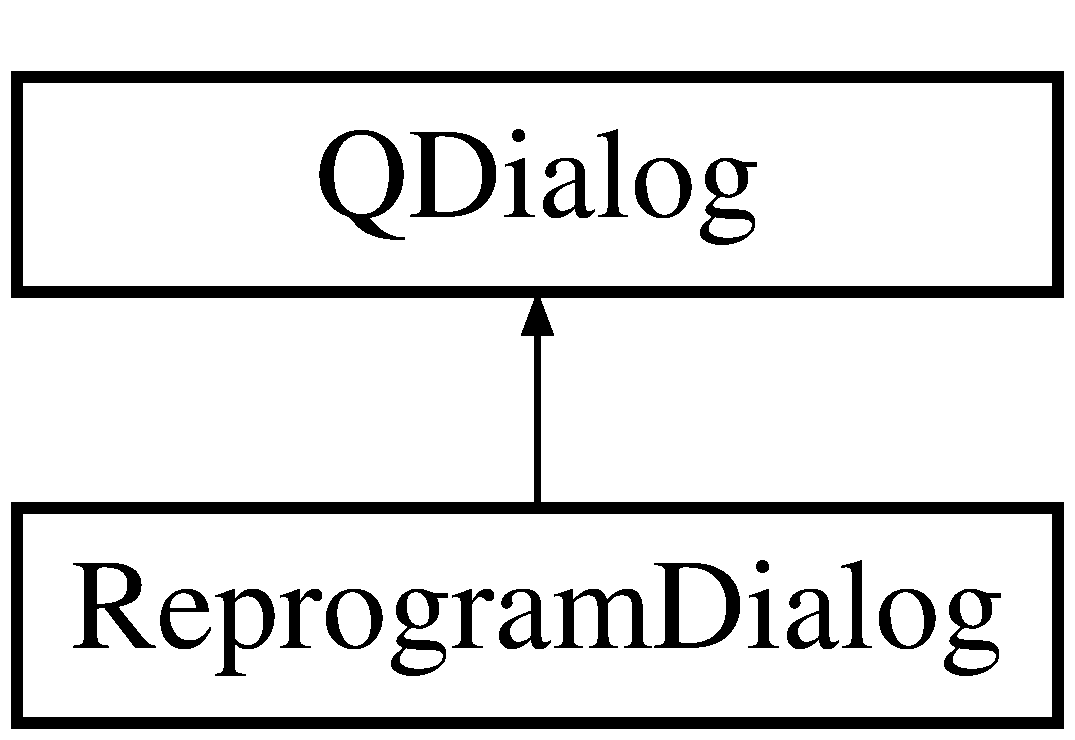
\includegraphics[height=2.000000cm]{classReprogramDialog}
\end{center}
\end{figure}
\subsubsection*{Public Types}
\begin{DoxyCompactItemize}
\item 
enum \mbox{\hyperlink{classReprogramDialog_a068bfc2d12863d24912b9ead24679b4a}{Board\+Type\+\_\+}} \{
\begin{DoxyCompactItemize} \item\mbox{\hyperlink{classReprogramDialog_a068bfc2d12863d24912b9ead24679b4aa384bf879731c24c01d00697b7f9daae9}{Master\+\_\+\+A\+T\+Xmega}}, 
\item\mbox{\hyperlink{classReprogramDialog_a068bfc2d12863d24912b9ead24679b4aaa55ff2104b7e7442625068c67e776d7e}{Heads\+\_\+\+A\+T\+Xmega}}, 
\item\mbox{\hyperlink{classReprogramDialog_a068bfc2d12863d24912b9ead24679b4aa2387446a69abe0ec84b008897037cb75}{Master\+\_\+\+A\+Tmega}}, 
\item\mbox{\hyperlink{classReprogramDialog_a068bfc2d12863d24912b9ead24679b4aaf3e17588a0c29e9b10dda1f9e3df9f6c}{Heads\+\_\+\+A\+Tmega}}
\end{DoxyCompactItemize}
 \}
\item 
typedef enum \mbox{\hyperlink{classReprogramDialog_a068bfc2d12863d24912b9ead24679b4a}{Reprogram\+Dialog\+::\+Board\+Type\+\_\+}} \mbox{\hyperlink{classReprogramDialog_a95e0c039a5de1ea8d3ad44a6ccf17b6a}{Board\+Type}}
\end{DoxyCompactItemize}
\subsubsection*{Public Slots}
\begin{DoxyCompactItemize}
\item 
void \mbox{\hyperlink{classReprogramDialog_a8aae6616889329598369a881496598ff}{set\+Progress}} (int progress)
\end{DoxyCompactItemize}
\subsubsection*{Signals}
\begin{DoxyCompactItemize}
\item 
void \mbox{\hyperlink{classReprogramDialog_a8a1f5e9816d7832931dc1da19c57b3ba}{program\+Arr\+Ready}} (\mbox{\hyperlink{classReprogramDialog_a95e0c039a5de1ea8d3ad44a6ccf17b6a}{Reprogram\+Dialog\+::\+Board\+Type}} type, Q\+Byte\+Array prog\+Arr)
\end{DoxyCompactItemize}
\subsubsection*{Public Member Functions}
\begin{DoxyCompactItemize}
\item 
\mbox{\hyperlink{classReprogramDialog_ac3f5b1fbef23169fc841a4108aecb834}{Reprogram\+Dialog}} (Q\+Widget $\ast$parent=0)
\item 
\mbox{\hyperlink{classReprogramDialog_a5b8aa028f9c61b2c12c17242402c2199}{$\sim$\+Reprogram\+Dialog}} ()
\end{DoxyCompactItemize}
\subsubsection*{Private Slots}
\begin{DoxyCompactItemize}
\item 
void \mbox{\hyperlink{classReprogramDialog_a2b95a979bdf73a8c885446e483f272ac}{on\+\_\+push\+Button\+Open\+File\+\_\+clicked}} ()
\item 
void \mbox{\hyperlink{classReprogramDialog_a0180445b000071fee4185f70a264a418}{on\+\_\+push\+Button\+Erase\+\_\+clicked}} ()
\item 
void \mbox{\hyperlink{classReprogramDialog_a5db4a9ac21377a1a5f39c3eaa2a27a4e}{on\+\_\+push\+Button\+Write\+\_\+clicked}} ()
\end{DoxyCompactItemize}
\subsubsection*{Private Attributes}
\begin{DoxyCompactItemize}
\item 
Ui\+::\+Reprogram\+Dialog $\ast$ \mbox{\hyperlink{classReprogramDialog_a0adb9c63d59d13d77203e334ec321b49}{ui}}
\item 
Q\+File \mbox{\hyperlink{classReprogramDialog_aeb56932944b2f861acffa0ab72a5a54f}{in\+File}}
\item 
Q\+String \mbox{\hyperlink{classReprogramDialog_ae56bcc760f9b1b305dc80756e7592ad7}{in\+File\+Name}}
\item 
Q\+Byte\+Array \mbox{\hyperlink{classReprogramDialog_ae9a10d87b7aa4dea0b6068ad6c336913}{program\+Arr}}
\end{DoxyCompactItemize}


\subsubsection{Member Typedef Documentation}
\mbox{\Hypertarget{classReprogramDialog_a95e0c039a5de1ea8d3ad44a6ccf17b6a}\label{classReprogramDialog_a95e0c039a5de1ea8d3ad44a6ccf17b6a}} 
\index{Reprogram\+Dialog@{Reprogram\+Dialog}!Board\+Type@{Board\+Type}}
\index{Board\+Type@{Board\+Type}!Reprogram\+Dialog@{Reprogram\+Dialog}}
{\footnotesize\ttfamily typedef enum \mbox{\hyperlink{classReprogramDialog_a068bfc2d12863d24912b9ead24679b4a}{Reprogram\+Dialog\+::\+Board\+Type\+\_\+}} \mbox{\hyperlink{classReprogramDialog_a95e0c039a5de1ea8d3ad44a6ccf17b6a}{Reprogram\+Dialog\+::\texorpdfstring{Board\+Type}{BoardType}}}} - describe type of processor and type of device which will be reprogrammed by this module.


\subsubsection{Member Enumeration Documentation}
\mbox{\Hypertarget{classReprogramDialog_a068bfc2d12863d24912b9ead24679b4a}\label{classReprogramDialog_a068bfc2d12863d24912b9ead24679b4a}} 
\index{Reprogram\+Dialog@{Reprogram\+Dialog}!Board\+Type\+\_\+@{Board\+Type\+\_\+}}
\index{Board\+Type\+\_\+@{Board\+Type\+\_\+}!Reprogram\+Dialog@{Reprogram\+Dialog}}
{\footnotesize\ttfamily enum \mbox{\hyperlink{classReprogramDialog_a068bfc2d12863d24912b9ead24679b4a}{Reprogram\+Dialog\+::\texorpdfstring{Board\+Type\+\_\+}{BoardType\_}}}}

\begin{DoxyEnumFields}{Enumerator}
\raisebox{\heightof{T}}[0pt][0pt]{\index{Master\+\_\+\+A\+T\+Xmega@{Master\+\_\+\+A\+T\+Xmega}!Reprogram\+Dialog@{Reprogram\+Dialog}}\index{Reprogram\+Dialog@{Reprogram\+Dialog}!Master\+\_\+\+A\+T\+Xmega@{Master\+\_\+\+A\+T\+Xmega}}}\mbox{\Hypertarget{classReprogramDialog_a068bfc2d12863d24912b9ead24679b4aa384bf879731c24c01d00697b7f9daae9}\label{classReprogramDialog_a068bfc2d12863d24912b9ead24679b4aa384bf879731c24c01d00697b7f9daae9}} 
Master\+\_\+\+A\+T\+Xmega&0x00\\
\hline

\raisebox{\heightof{T}}[0pt][0pt]{\index{Heads\+\_\+\+A\+T\+Xmega@{Heads\+\_\+\+A\+T\+Xmega}!Reprogram\+Dialog@{Reprogram\+Dialog}}\index{Reprogram\+Dialog@{Reprogram\+Dialog}!Heads\+\_\+\+A\+T\+Xmega@{Heads\+\_\+\+A\+T\+Xmega}}}\mbox{\Hypertarget{classReprogramDialog_a068bfc2d12863d24912b9ead24679b4aaa55ff2104b7e7442625068c67e776d7e}\label{classReprogramDialog_a068bfc2d12863d24912b9ead24679b4aaa55ff2104b7e7442625068c67e776d7e}} 
Heads\+\_\+\+A\+T\+Xmega& 0x01\\
\hline

\raisebox{\heightof{T}}[0pt][0pt]{\index{Master\+\_\+\+A\+Tmega@{Master\+\_\+\+A\+Tmega}!Reprogram\+Dialog@{Reprogram\+Dialog}}\index{Reprogram\+Dialog@{Reprogram\+Dialog}!Master\+\_\+\+A\+Tmega@{Master\+\_\+\+A\+Tmega}}}\mbox{\Hypertarget{classReprogramDialog_a068bfc2d12863d24912b9ead24679b4aa2387446a69abe0ec84b008897037cb75}\label{classReprogramDialog_a068bfc2d12863d24912b9ead24679b4aa2387446a69abe0ec84b008897037cb75}} 
Master\+\_\+\+A\+Tmega&0x02\\
\hline

\raisebox{\heightof{T}}[0pt][0pt]{\index{Heads\+\_\+\+A\+Tmega@{Heads\+\_\+\+A\+Tmega}!Reprogram\+Dialog@{Reprogram\+Dialog}}\index{Reprogram\+Dialog@{Reprogram\+Dialog}!Heads\+\_\+\+A\+Tmega@{Heads\+\_\+\+A\+Tmega}}}\mbox{\Hypertarget{classReprogramDialog_a068bfc2d12863d24912b9ead24679b4aaf3e17588a0c29e9b10dda1f9e3df9f6c}\label{classReprogramDialog_a068bfc2d12863d24912b9ead24679b4aaf3e17588a0c29e9b10dda1f9e3df9f6c}} 
Heads\+\_\+\+A\+Tmega&0x03\\
\hline

\end{DoxyEnumFields}


\subsubsection{Constructor \& Destructor Documentation}
\mbox{\Hypertarget{classReprogramDialog_ac3f5b1fbef23169fc841a4108aecb834}\label{classReprogramDialog_ac3f5b1fbef23169fc841a4108aecb834}} 
\index{Reprogram\+Dialog@{Reprogram\+Dialog}!Reprogram\+Dialog@{Reprogram\+Dialog}}
\index{Reprogram\+Dialog@{Reprogram\+Dialog}!Reprogram\+Dialog@{Reprogram\+Dialog}}
{\footnotesize\ttfamily Reprogram\+Dialog\+::\texorpdfstring{Reprogram\+Dialog}{ReprogramDialog} (\begin{DoxyParamCaption}\item[{Q\+Widget $\ast$}]{parent = {\ttfamily 0} }\end{DoxyParamCaption})\hspace{0.3cm}{\ttfamily [explicit]}} - standard Q\+Widget constructor.

\mbox{\Hypertarget{classReprogramDialog_a5b8aa028f9c61b2c12c17242402c2199}\label{classReprogramDialog_a5b8aa028f9c61b2c12c17242402c2199}} 
\index{Reprogram\+Dialog@{Reprogram\+Dialog}!````~Reprogram\+Dialog@{$\sim$\+Reprogram\+Dialog}}
\index{````~Reprogram\+Dialog@{$\sim$\+Reprogram\+Dialog}!Reprogram\+Dialog@{Reprogram\+Dialog}}
{\footnotesize\ttfamily Reprogram\+Dialog\+::\texorpdfstring{$\sim$\+Reprogram\+Dialog}{~ReprogramDialog} (\begin{DoxyParamCaption}{ }\end{DoxyParamCaption})} - standard Q\+Widget destructor.



\subsubsection{Member Function Documentation}
\mbox{\Hypertarget{classReprogramDialog_a0180445b000071fee4185f70a264a418}\label{classReprogramDialog_a0180445b000071fee4185f70a264a418}} 
\index{Reprogram\+Dialog@{Reprogram\+Dialog}!on\+\_\+push\+Button\+Erase\+\_\+clicked@{on\+\_\+push\+Button\+Erase\+\_\+clicked}}
\index{on\+\_\+push\+Button\+Erase\+\_\+clicked@{on\+\_\+push\+Button\+Erase\+\_\+clicked}!Reprogram\+Dialog@{Reprogram\+Dialog}}
{\footnotesize\ttfamily void Reprogram\+Dialog\+::\texorpdfstring{on\+\_\+push\+Button\+Erase\+\_\+clicked}{on\_pushButtonErase\_clicked} (\begin{DoxyParamCaption}{ }\end{DoxyParamCaption})\hspace{0.3cm}{\ttfamily [private]}, {\ttfamily [slot]}} - function to emit \hyperlink{classReprogramDialog_a8a1f5e9816d7832931dc1da19c57b3ba}{program\+Arr\+Ready}(...) with \textit{prog\+Arr} filled with zeros. 

\mbox{\Hypertarget{classReprogramDialog_a2b95a979bdf73a8c885446e483f272ac}\label{classReprogramDialog_a2b95a979bdf73a8c885446e483f272ac}} 
\index{Reprogram\+Dialog@{Reprogram\+Dialog}!on\+\_\+push\+Button\+Open\+File\+\_\+clicked@{on\+\_\+push\+Button\+Open\+File\+\_\+clicked}}
\index{on\+\_\+push\+Button\+Open\+File\+\_\+clicked@{on\+\_\+push\+Button\+Open\+File\+\_\+clicked}!Reprogram\+Dialog@{Reprogram\+Dialog}}
{\footnotesize\ttfamily void Reprogram\+Dialog\+::\texorpdfstring{on\+\_\+push\+Button\+Open\+File\+\_\+clicked}{on\_pushButtonOpenFile\_clicked} (\begin{DoxyParamCaption}{ }\end{DoxyParamCaption})\hspace{0.3cm}{\ttfamily [private]}, {\ttfamily [slot]}} - function to open text-HEX file with program in Intel-hex format, set value of \hyperlink{classReprogramDialog_ae56bcc760f9b1b305dc80756e7592ad7}{in\+File\+Name} and set file name of \hyperlink{classReprogramDialog_aeb56932944b2f861acffa0ab72a5a54f}{in\+File}.

\mbox{\Hypertarget{classReprogramDialog_a5db4a9ac21377a1a5f39c3eaa2a27a4e}\label{classReprogramDialog_a5db4a9ac21377a1a5f39c3eaa2a27a4e}} 
\index{Reprogram\+Dialog@{Reprogram\+Dialog}!on\+\_\+push\+Button\+Write\+\_\+clicked@{on\+\_\+push\+Button\+Write\+\_\+clicked}}
\index{on\+\_\+push\+Button\+Write\+\_\+clicked@{on\+\_\+push\+Button\+Write\+\_\+clicked}!Reprogram\+Dialog@{Reprogram\+Dialog}}
{\footnotesize\ttfamily void Reprogram\+Dialog\+::\texorpdfstring{on\+\_\+push\+Button\+Write\+\_\+clicked}{on\_pushButtonWrite\_clicked} (\begin{DoxyParamCaption}{ }\end{DoxyParamCaption})\hspace{0.3cm}{\ttfamily [private]}, {\ttfamily [slot]}} - function which used for open \hyperlink{classReprogramDialog_aeb56932944b2f861acffa0ab72a5a54f}{in\+File}, read text from it and fill \hyperlink{classReprogramDialog_ae9a10d87b7aa4dea0b6068ad6c336913}{program\+Arr} with hex data to write it into devices. After that function emit \hyperlink{classReprogramDialog_a8a1f5e9816d7832931dc1da19c57b3ba}{program\+Arr\+Ready}(...) signal with appropriate parameters. 

\mbox{\Hypertarget{classReprogramDialog_a8a1f5e9816d7832931dc1da19c57b3ba}\label{classReprogramDialog_a8a1f5e9816d7832931dc1da19c57b3ba}} 
\index{Reprogram\+Dialog@{Reprogram\+Dialog}!program\+Arr\+Ready@{program\+Arr\+Ready}}
\index{program\+Arr\+Ready@{program\+Arr\+Ready}!Reprogram\+Dialog@{Reprogram\+Dialog}}
{\footnotesize\ttfamily void Reprogram\+Dialog\+::\texorpdfstring{program\+Arr\+Ready}{programArrReady} (\begin{DoxyParamCaption}\item[{\mbox{\hyperlink{classReprogramDialog_a95e0c039a5de1ea8d3ad44a6ccf17b6a}{Reprogram\+Dialog\+::\+Board\+Type}}}]{type,  }\item[{Q\+Byte\+Array}]{prog\+Arr }\end{DoxyParamCaption})\hspace{0.3cm}{\ttfamily [signal]}} - signal which emitted by \hyperlink{classReprogramDialog_a0180445b000071fee4185f70a264a418}{on\+\_\+push\+Button\+Erase\+\_\+clicked}(...) and \hyperlink{classReprogramDialog_a5db4a9ac21377a1a5f39c3eaa2a27a4e}{on\+\_\+push\+Button\+Write\+\_\+clicked}(...) functions and handle in parent object.

\mbox{\Hypertarget{classReprogramDialog_a8aae6616889329598369a881496598ff}\label{classReprogramDialog_a8aae6616889329598369a881496598ff}} 
\index{Reprogram\+Dialog@{Reprogram\+Dialog}!set\+Progress@{set\+Progress}}
\index{set\+Progress@{set\+Progress}!Reprogram\+Dialog@{Reprogram\+Dialog}}
{\footnotesize\ttfamily void Reprogram\+Dialog\+::\texorpdfstring{set\+Progress}{setProgress} (\begin{DoxyParamCaption}\item[{int}]{progress }\end{DoxyParamCaption})\hspace{0.3cm}{\ttfamily [slot]}} - function to set value of programming process at dialog.



\subsubsection{Member Data Documentation}
\mbox{\Hypertarget{classReprogramDialog_aeb56932944b2f861acffa0ab72a5a54f}\label{classReprogramDialog_aeb56932944b2f861acffa0ab72a5a54f}} 
\index{Reprogram\+Dialog@{Reprogram\+Dialog}!in\+File@{in\+File}}
\index{in\+File@{in\+File}!Reprogram\+Dialog@{Reprogram\+Dialog}}
{\footnotesize\ttfamily Q\+File Reprogram\+Dialog\+::\texorpdfstring{in\+File}{inFile}\hspace{0.3cm}{\ttfamily [private]}}

\mbox{\Hypertarget{classReprogramDialog_ae56bcc760f9b1b305dc80756e7592ad7}\label{classReprogramDialog_ae56bcc760f9b1b305dc80756e7592ad7}} 
\index{Reprogram\+Dialog@{Reprogram\+Dialog}!in\+File\+Name@{in\+File\+Name}}
\index{in\+File\+Name@{in\+File\+Name}!Reprogram\+Dialog@{Reprogram\+Dialog}}
{\footnotesize\ttfamily Q\+String Reprogram\+Dialog\+::\texorpdfstring{in\+File\+Name}{inFileName}\hspace{0.3cm}{\ttfamily [private]}}

\mbox{\Hypertarget{classReprogramDialog_ae9a10d87b7aa4dea0b6068ad6c336913}\label{classReprogramDialog_ae9a10d87b7aa4dea0b6068ad6c336913}} 
\index{Reprogram\+Dialog@{Reprogram\+Dialog}!program\+Arr@{program\+Arr}}
\index{program\+Arr@{program\+Arr}!Reprogram\+Dialog@{Reprogram\+Dialog}}
{\footnotesize\ttfamily Q\+Byte\+Array Reprogram\+Dialog\+::\texorpdfstring{program\+Arr}{programArr}\hspace{0.3cm}{\ttfamily [private]}}


The documentation for this class was generated from the following files\+:\begin{DoxyCompactItemize}
\item 
\mbox{\hyperlink{reprogramdialog_8h}{reprogramdialog.\+h}}\item 
\mbox{\hyperlink{reprogramdialog_8cpp}{reprogramdialog.\+cpp}}\end{DoxyCompactItemize}
\newpage
\hypertarget{classSerialPort}{}\subsection{Serial\+Port Class Reference}
\label{classSerialPort}\index{Serial\+Port@{Serial\+Port}}


{\ttfamily \#include $<$serialport.\+h$>$}

Inheritance diagram for Serial\+Port\+:\begin{figure}[H]
\begin{center}
\leavevmode
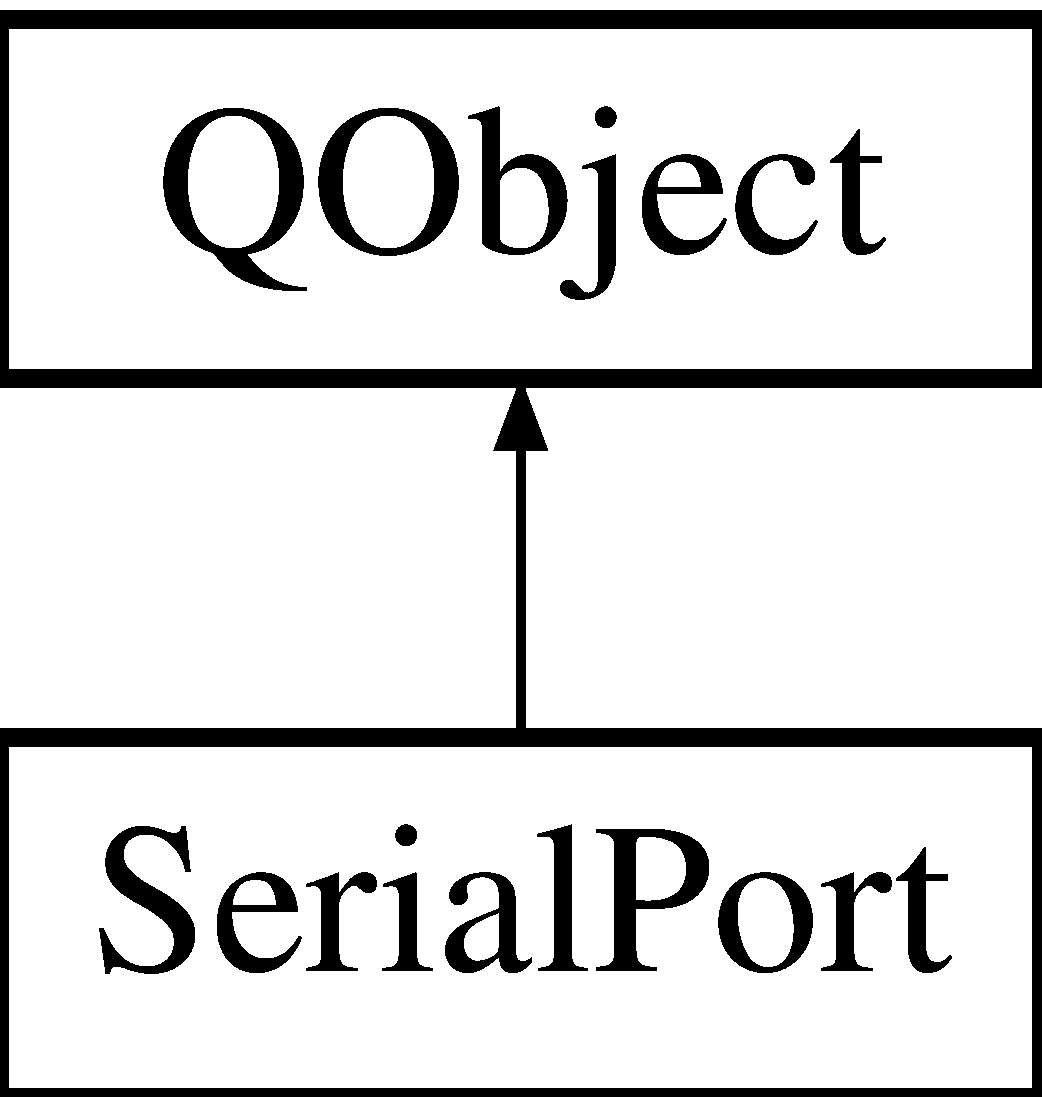
\includegraphics[height=2.000000cm]{classSerialPort}
\end{center}
\end{figure}
\subsubsection*{Public Slots}
\begin{DoxyCompactItemize}
\item 
void \mbox{\hyperlink{classSerialPort_ab831db6582a7b576adf5059555e0297f}{open\+Serial\+Port}} ()
\item 
void \mbox{\hyperlink{classSerialPort_ac4f59ca6f1401ed8bbc6de3f99cfa411}{open\+Serial\+Port}} (\mbox{\hyperlink{structComSettings}{Com\+Settings}} c\+Sett)
\item 
void \mbox{\hyperlink{classSerialPort_a075482970cd99f66457eac471127a710}{close\+Serial\+Port}} ()
\item 
void \mbox{\hyperlink{classSerialPort_adc2e6d59b77389c9047aab5bb1ebd5dc}{send\+Program}} (\mbox{\hyperlink{classReprogramDialog_a95e0c039a5de1ea8d3ad44a6ccf17b6a}{Reprogram\+Dialog\+::\+Board\+Type}} type, Q\+Byte\+Array program\+Arr)
\item 
void \mbox{\hyperlink{classSerialPort_a2616700b4daafeb521f222e7d846dc99}{send\+Data}} (Q\+Byte\+Array data, bool send=false, bool half\+Byte=false)
\item 
void \mbox{\hyperlink{classSerialPort_a412616b006e1b16efaf6ffd480cb9cc0}{send\+Mod\+Data}} (\mbox{\hyperlink{settings_8h_a48091a1e52849b0871df2f7081be2e38}{uint8\+\_\+t}} dev, \mbox{\hyperlink{settings_8h_a48091a1e52849b0871df2f7081be2e38}{uint8\+\_\+t}} place, \mbox{\hyperlink{settings_8h_a017dd44e68049ffdd31500a8cd01ba68}{uint16\+\_\+t}} data)
\item 
void \mbox{\hyperlink{classSerialPort_afe266bc6e1641be604b5d97c88910bc4}{send\+Reg}} (\mbox{\hyperlink{settings_8h_a48091a1e52849b0871df2f7081be2e38}{uint8\+\_\+t}} dev, \mbox{\hyperlink{settings_8h_a48091a1e52849b0871df2f7081be2e38}{uint8\+\_\+t}} place)
\item 
void \mbox{\hyperlink{classSerialPort_adf0c6d9bd0a312ae0e921085497fa8b4}{setup\+Port}} ()
\item 
void \mbox{\hyperlink{classSerialPort_ab723ad9ecd8571d2156ad9b141cfd24e}{set\+Com\+Params}} (\mbox{\hyperlink{structComSettings}{Com\+Settings}} sett)
\item 
void \mbox{\hyperlink{classSerialPort_a7dbba05770c1fd93db1026c0e5cc12a7}{set\+Style\+Sheet}} (Q\+String st\+Sheet)
\end{DoxyCompactItemize}
\subsubsection*{Signals}
\begin{DoxyCompactItemize}
\item 
void \mbox{\hyperlink{classSerialPort_a4653f9aa7114546faa5627ee5810a47d}{data\+Ready}} (Q\+Byte\+Array data)
\item 
void \mbox{\hyperlink{classSerialPort_aa958ae188335f80fd08ebad93e977134}{data\+Ready}} (\mbox{\hyperlink{serialport_8h_a2331c0232719069f0bce03c249d2eec6}{Mod\+Data}} mod\+Data)
\item 
void \mbox{\hyperlink{classSerialPort_a30f185f507d89b40a0204b6472da3217}{serial\+Setting\+Accepted}} (\mbox{\hyperlink{structComSettings}{Com\+Settings}} seittngs)
\item 
void \mbox{\hyperlink{classSerialPort_ae92426fd329e2a5ec42b0255c5dcbdc5}{working}} ()
\item 
void \mbox{\hyperlink{classSerialPort_a38b94a606dab2af9cbeac4f48ddd831c}{proram\+Progres}} (int progres)
\end{DoxyCompactItemize}
\subsubsection*{Public Member Functions}
\begin{DoxyCompactItemize}
\item 
\mbox{\hyperlink{classSerialPort_ae68e4a28e607b4acbab2c2a894cb3e2b}{Serial\+Port}} (Q\+Object $\ast$parent=0)
\item 
\mbox{\hyperlink{classSerialPort_aa9fb64a8aced84ab80eee65680298976}{Serial\+Port}} (\mbox{\hyperlink{structComSettings}{Com\+Settings}} settings, Q\+Object $\ast$parent=0)
\item 
void \mbox{\hyperlink{classSerialPort_a273c33e0eac534d7bdeafed79157e2e4}{set\+Register\+Pointer}} (\mbox{\hyperlink{classRegister}{Register}} $\ast$reg\+Ptr)
\end{DoxyCompactItemize}
\subsubsection*{Private Slots}
\begin{DoxyCompactItemize}
\item 
void \mbox{\hyperlink{classSerialPort_a0b8fe1371e829199856e8cae942de94e}{read\+Data}} ()
\item 
void \mbox{\hyperlink{classSerialPort_a307128aa2e5ad6b89e47898bff7a48e0}{handle\+Error}} (Q\+Serial\+Port\+::\+Serial\+Port\+Error error)
\item 
void \mbox{\hyperlink{classSerialPort_a9153ab33cbb73d5138b871e52c343e58}{show\+Status\+Message}} (const Q\+String \&message)
\item 
void \mbox{\hyperlink{classSerialPort_a39602f4cf8fe4570fa3b69d633534be5}{get\+Serial\+Setting}} (\mbox{\hyperlink{structComSettings}{Com\+Settings}} setting)
\end{DoxyCompactItemize}
\subsubsection*{Private Member Functions}
\begin{DoxyCompactItemize}
\item 
Q\+Byte\+Array \mbox{\hyperlink{classSerialPort_a8be1b40710483fea19e272b04568f14e}{data\+Transform}} (Q\+Byte\+Array data)
\end{DoxyCompactItemize}
\subsubsection*{Private Attributes}
\begin{DoxyCompactItemize}
\item 
\mbox{\hyperlink{classSerialSettingsDialog}{Serial\+Settings\+Dialog}} $\ast$ \mbox{\hyperlink{classSerialPort_a9ab445f818748122d3368fd2e9dbbbea}{settings\+Com\+Dialog}}
\item 
Q\+Serial\+Port $\ast$ \mbox{\hyperlink{classSerialPort_a54120d9040537e637eae7e8c048dec31}{serial}}
\item 
\mbox{\hyperlink{classRegister}{Register}} $\ast$ \mbox{\hyperlink{classSerialPort_ab98c7d39235d59c2086d9f6e94c3ed4b}{registers}}
\item 
\mbox{\hyperlink{serialport_8h_a2331c0232719069f0bce03c249d2eec6}{Mod\+Data}} \mbox{\hyperlink{classSerialPort_a1fbdedb09ef8f5d7ecb4e43e848d025f}{mod\+Data8}}
\item 
Q\+Byte\+Array \mbox{\hyperlink{classSerialPort_abc55095109004eb5e21e923c25036549}{data\+To\+Send\+Buff}}
\item 
int \mbox{\hyperlink{classSerialPort_a97937bbe34853205cbd02fb5ff97653d}{reply\+Cnt}}
\item 
bool \mbox{\hyperlink{classSerialPort_adf375ee179fa4844cadf65645ee7ab2f}{init\+App}}
\end{DoxyCompactItemize}


\subsubsection{Constructor \& Destructor Documentation}
\mbox{\Hypertarget{classSerialPort_ae68e4a28e607b4acbab2c2a894cb3e2b}\label{classSerialPort_ae68e4a28e607b4acbab2c2a894cb3e2b}} 
\index{Serial\+Port@{Serial\+Port}!Serial\+Port@{Serial\+Port}}
\index{Serial\+Port@{Serial\+Port}!Serial\+Port@{Serial\+Port}}
{\footnotesize\ttfamily Serial\+Port\+::\texorpdfstring{Serial\+Port}{SerialPort}{\footnotesize\ttfamily [1/2]} (\begin{DoxyParamCaption}\item[{Q\+Object $\ast$}]{parent = {\ttfamily 0} }\end{DoxyParamCaption})\hspace{0.3cm}{\ttfamily [explicit]}} - first variant of polymorphic constructor of class. Create Q\+Serial\+Port class object and \hyperlink{classSerialSettingsDialog}{Serial\+Settings\+Dialog} class object with default parameters.

\mbox{\Hypertarget{classSerialPort_aa9fb64a8aced84ab80eee65680298976}\label{classSerialPort_aa9fb64a8aced84ab80eee65680298976}} 
\index{Serial\+Port@{Serial\+Port}!Serial\+Port@{Serial\+Port}}
\index{Serial\+Port@{Serial\+Port}!Serial\+Port@{Serial\+Port}}
{\footnotesize\ttfamily Serial\+Port\+::\texorpdfstring{Serial\+Port()}{SerialPort()}{\footnotesize\ttfamily [2/2]} (\begin{DoxyParamCaption}\item[{\mbox{\hyperlink{structComSettings}{Com\+Settings}}}]{settings,  }\item[{Q\+Object $\ast$}]{parent = {\ttfamily 0} }\end{DoxyParamCaption})\hspace{0.3cm}{\ttfamily [explicit]}} - second variant of polymorphic constructor of class. Create Q\+Serial\+Port class object and \hyperlink{classSerialSettingsDialog}{Serial\+Settings\+Dialog} class object with given at \textit{settings} parameters.



\subsubsection{Member Function Documentation}
\mbox{\Hypertarget{classSerialPort_a075482970cd99f66457eac471127a710}\label{classSerialPort_a075482970cd99f66457eac471127a710}} 
\index{Serial\+Port@{Serial\+Port}!close\+Serial\+Port@{close\+Serial\+Port}}
\index{close\+Serial\+Port@{close\+Serial\+Port}!Serial\+Port@{Serial\+Port}}
{\footnotesize\ttfamily void Serial\+Port\+::\texorpdfstring{close\+Serial\+Port}{closeSerialPort} (\begin{DoxyParamCaption}{ }\end{DoxyParamCaption})\hspace{0.3cm}{\ttfamily [slot]}} - function to close \hyperlink{classSerialPort_a54120d9040537e637eae7e8c048dec31}{serial} port if it's open.

\mbox{\Hypertarget{classSerialPort_a4653f9aa7114546faa5627ee5810a47d}\label{classSerialPort_a4653f9aa7114546faa5627ee5810a47d}} 
\index{Serial\+Port@{Serial\+Port}!data\+Ready@{data\+Ready}}
\index{data\+Ready@{data\+Ready}!Serial\+Port@{Serial\+Port}}
{\footnotesize\ttfamily void Serial\+Port\+::\texorpdfstring{data\+Ready}{dataReady}{\footnotesize\ttfamily [1/2]} (\begin{DoxyParamCaption}\item[{Q\+Byte\+Array}]{data }\end{DoxyParamCaption})\hspace{0.3cm}{\ttfamily [signal]}} - signal which emits by \hyperlink{classSerialPort_a0b8fe1371e829199856e8cae942de94e}{read\+Data}(...) function. Signal contain byte array with data after C\+R\+C check.

\mbox{\Hypertarget{classSerialPort_aa958ae188335f80fd08ebad93e977134}\label{classSerialPort_aa958ae188335f80fd08ebad93e977134}} 
\index{Serial\+Port@{Serial\+Port}!data\+Ready@{data\+Ready}}
\index{data\+Ready@{data\+Ready}!Serial\+Port@{Serial\+Port}}
{\footnotesize\ttfamily void Serial\+Port\+::\texorpdfstring{data\+Ready}{dataReady}{\footnotesize\ttfamily [2/2]} (\begin{DoxyParamCaption}\item[{\mbox{\hyperlink{serialport_8h_a2331c0232719069f0bce03c249d2eec6}{Mod\+Data}}}]{mod\+Data }\end{DoxyParamCaption})\hspace{0.3cm}{\ttfamily [signal]}} - signal which emits by \hyperlink{classSerialPort_a0b8fe1371e829199856e8cae942de94e}{read\+Data}(...) function. Signal contain \textit{mod\+Data} after C\+R\+C check.

\mbox{\Hypertarget{classSerialPort_a8be1b40710483fea19e272b04568f14e}\label{classSerialPort_a8be1b40710483fea19e272b04568f14e}} 
\index{Serial\+Port@{Serial\+Port}!data\+Transform@{data\+Transform}}
\index{data\+Transform@{data\+Transform}!Serial\+Port@{Serial\+Port}}
{\footnotesize\ttfamily Q\+Byte\+Array Serial\+Port\+::\texorpdfstring{data\+Transform}{dataTransform} (\begin{DoxyParamCaption}\item[{Q\+Byte\+Array}]{data }\end{DoxyParamCaption})\hspace{0.3cm}{\ttfamily [private]}} - function to transform data from half-byte to full-byte array.

\mbox{\Hypertarget{classSerialPort_a39602f4cf8fe4570fa3b69d633534be5}\label{classSerialPort_a39602f4cf8fe4570fa3b69d633534be5}} 
\index{Serial\+Port@{Serial\+Port}!get\+Serial\+Setting@{get\+Serial\+Setting}}
\index{get\+Serial\+Setting@{get\+Serial\+Setting}!Serial\+Port@{Serial\+Port}}
{\footnotesize\ttfamily void Serial\+Port\+::\texorpdfstring{get\+Serial\+Setting}{getSerialSetting} (\begin{DoxyParamCaption}\item[{\mbox{\hyperlink{structComSettings}{Com\+Settings}}}]{setting }\end{DoxyParamCaption})\hspace{0.3cm}{\ttfamily [private]}, {\ttfamily [slot]}} - function to emit \hyperlink{classSerialPort_a30f185f507d89b40a0204b6472da3217}{serial\+Setting\+Accepted}(...) signal to save serial settings to hard drive. 

\mbox{\Hypertarget{classSerialPort_a307128aa2e5ad6b89e47898bff7a48e0}\label{classSerialPort_a307128aa2e5ad6b89e47898bff7a48e0}} 
\index{Serial\+Port@{Serial\+Port}!handle\+Error@{handle\+Error}}
\index{handle\+Error@{handle\+Error}!Serial\+Port@{Serial\+Port}}
{\footnotesize\ttfamily void Serial\+Port\+::\texorpdfstring{handle\+Error}{handleError} (\begin{DoxyParamCaption}\item[{Q\+Serial\+Port\+::\+Serial\+Port\+Error}]{error }\end{DoxyParamCaption})\hspace{0.3cm}{\ttfamily [private]}, {\ttfamily [slot]}} - serial port errors handler. Used to show Q\+Message\+Box with error text.

\mbox{\Hypertarget{classSerialPort_ab831db6582a7b576adf5059555e0297f}\label{classSerialPort_ab831db6582a7b576adf5059555e0297f}} 
\index{Serial\+Port@{Serial\+Port}!open\+Serial\+Port@{open\+Serial\+Port}}
\index{open\+Serial\+Port@{open\+Serial\+Port}!Serial\+Port@{Serial\+Port}}
{\footnotesize\ttfamily void Serial\+Port\+::\texorpdfstring{open\+Serial\+Port}{openSerialPort}{\footnotesize\ttfamily [1/2]} (\begin{DoxyParamCaption}{ }\end{DoxyParamCaption})\hspace{0.3cm}{\ttfamily [slot]}} - function to open serial port with \hyperlink{classSerialPort_a9ab445f818748122d3368fd2e9dbbbea}{settings\+Com\+Dialog}->\hyperlink{classSerialSettingsDialog_ab24259a0385b292ff104425d97957482}{current\+Settings} 

\mbox{\Hypertarget{classSerialPort_ac4f59ca6f1401ed8bbc6de3f99cfa411}\label{classSerialPort_ac4f59ca6f1401ed8bbc6de3f99cfa411}} 
\index{Serial\+Port@{Serial\+Port}!open\+Serial\+Port@{open\+Serial\+Port}}
\index{open\+Serial\+Port@{open\+Serial\+Port}!Serial\+Port@{Serial\+Port}}
{\footnotesize\ttfamily void Serial\+Port\+::\texorpdfstring{open\+Serial\+Port}{openSerialPort}{\footnotesize\ttfamily [2/2]} (\begin{DoxyParamCaption}\item[{\mbox{\hyperlink{structComSettings}{Com\+Settings}}}]{c\+Sett }\end{DoxyParamCaption})\hspace{0.3cm}{\ttfamily [slot]}} - function to open serial port with settings given in \textit{c\+Sett} variable.

\mbox{\Hypertarget{classSerialPort_a38b94a606dab2af9cbeac4f48ddd831c}\label{classSerialPort_a38b94a606dab2af9cbeac4f48ddd831c}} 
\index{Serial\+Port@{Serial\+Port}!proram\+Progres@{proram\+Progres}}
\index{proram\+Progres@{proram\+Progres}!Serial\+Port@{Serial\+Port}}
{\footnotesize\ttfamily void Serial\+Port\+::\texorpdfstring{proram\+Progres}{proramProgres} (\begin{DoxyParamCaption}\item[{int}]{progres }\end{DoxyParamCaption})\hspace{0.3cm}{\ttfamily [signal]}} - signal to send process of reprogramming PCB's. 

\mbox{\Hypertarget{classSerialPort_a0b8fe1371e829199856e8cae942de94e}\label{classSerialPort_a0b8fe1371e829199856e8cae942de94e}} 
\index{Serial\+Port@{Serial\+Port}!read\+Data@{read\+Data}}
\index{read\+Data@{read\+Data}!Serial\+Port@{Serial\+Port}}
{\footnotesize\ttfamily void Serial\+Port\+::\texorpdfstring{read\+Data}{readData} (\begin{DoxyParamCaption}{ }\end{DoxyParamCaption})\hspace{0.3cm}{\ttfamily [private]}, {\ttfamily [slot]}} - function to get data from serial port, analyze that data and create reply to send that to master PCB. 

\mbox{\Hypertarget{classSerialPort_a2616700b4daafeb521f222e7d846dc99}\label{classSerialPort_a2616700b4daafeb521f222e7d846dc99}} 
\index{Serial\+Port@{Serial\+Port}!send\+Data@{send\+Data}}
\index{send\+Data@{send\+Data}!Serial\+Port@{Serial\+Port}}
{\footnotesize\ttfamily void Serial\+Port\+::\texorpdfstring{send\+Data}{sendData} (\begin{DoxyParamCaption}\item[{Q\+Byte\+Array}]{data,  }\item[{bool}]{send = {\ttfamily false},  }\item[{bool}]{half\+Byte = {\ttfamily false} }\end{DoxyParamCaption})\hspace{0.3cm}{\ttfamily [slot]}} - function to send data to serial port. Function take \textit{data} to send it to \hyperlink{classSerialPort_a54120d9040537e637eae7e8c048dec31}{serial} port. Parameter \textit{send} describe way of data send: if \textit{true} than data sends immediately, if \textit{false} than data adding to \hyperlink{classSerialPort_abc55095109004eb5e21e923c25036549}{data\+To\+Send\+Buff} and send in it's turn. Parameter \textit{half\+Byte} specifies 	 requirement of data transformation - if \textit{true} data transform to half byte variant and sends after that, if \textit{false} data sends as it is.

\mbox{\Hypertarget{classSerialPort_a412616b006e1b16efaf6ffd480cb9cc0}\label{classSerialPort_a412616b006e1b16efaf6ffd480cb9cc0}} 
\index{Serial\+Port@{Serial\+Port}!send\+Mod\+Data@{send\+Mod\+Data}}
\index{send\+Mod\+Data@{send\+Mod\+Data}!Serial\+Port@{Serial\+Port}}
{\footnotesize\ttfamily void Serial\+Port\+::\texorpdfstring{send\+Mod\+Data}{sendModData} (\begin{DoxyParamCaption}\item[{\mbox{\hyperlink{settings_8h_a48091a1e52849b0871df2f7081be2e38}{uint8\+\_\+t}}}]{dev,  }\item[{\mbox{\hyperlink{settings_8h_a48091a1e52849b0871df2f7081be2e38}{uint8\+\_\+t}}}]{place,  }\item[{\mbox{\hyperlink{settings_8h_a017dd44e68049ffdd31500a8cd01ba68}{uint16\+\_\+t}}}]{data }\end{DoxyParamCaption})\hspace{0.3cm}{\ttfamily [slot]}} - function to send mod data to serial port. At function data gather to Q\+Byte\+Array and sends to serial port.

\mbox{\Hypertarget{classSerialPort_adc2e6d59b77389c9047aab5bb1ebd5dc}\label{classSerialPort_adc2e6d59b77389c9047aab5bb1ebd5dc}} 
\index{Serial\+Port@{Serial\+Port}!send\+Program@{send\+Program}}
\index{send\+Program@{send\+Program}!Serial\+Port@{Serial\+Port}}
{\footnotesize\ttfamily void Serial\+Port\+::\texorpdfstring{send\+Program}{sendProgram} (\begin{DoxyParamCaption}\item[{\mbox{\hyperlink{classReprogramDialog_a95e0c039a5de1ea8d3ad44a6ccf17b6a}{Reprogram\+Dialog\+::\+Board\+Type}}}]{type,  }\item[{Q\+Byte\+Array}]{program\+Arr }\end{DoxyParamCaption})\hspace{0.3cm}{\ttfamily [slot]}} - function to send \textit{program\+Arr} to PCB. Parameter \textit{type} describe which commands will be sends to start reprogramming and size of memory page.

\mbox{\Hypertarget{classSerialPort_afe266bc6e1641be604b5d97c88910bc4}\label{classSerialPort_afe266bc6e1641be604b5d97c88910bc4}} 
\index{Serial\+Port@{Serial\+Port}!send\+Reg@{send\+Reg}}
\index{send\+Reg@{send\+Reg}!Serial\+Port@{Serial\+Port}}
{\footnotesize\ttfamily void Serial\+Port\+::\texorpdfstring{send\+Reg}{sendReg} (\begin{DoxyParamCaption}\item[{\mbox{\hyperlink{settings_8h_a48091a1e52849b0871df2f7081be2e38}{uint8\+\_\+t}}}]{dev,  }\item[{\mbox{\hyperlink{settings_8h_a48091a1e52849b0871df2f7081be2e38}{uint8\+\_\+t}}}]{place }\end{DoxyParamCaption})\hspace{0.3cm}{\ttfamily [slot]}} - function to send data from \hyperlink{classSerialPort_ab98c7d39235d59c2086d9f6e94c3ed4b}{registers} at \textit{dev} and \textit{place}. At function data gather to Q\+Byte\+Array and sends to serial port.

\mbox{\Hypertarget{classSerialPort_a30f185f507d89b40a0204b6472da3217}\label{classSerialPort_a30f185f507d89b40a0204b6472da3217}} 
\index{Serial\+Port@{Serial\+Port}!serial\+Setting\+Accepted@{serial\+Setting\+Accepted}}
\index{serial\+Setting\+Accepted@{serial\+Setting\+Accepted}!Serial\+Port@{Serial\+Port}}
{\footnotesize\ttfamily void Serial\+Port\+::\texorpdfstring{serial\+Setting\+Accepted}{serialSettingAccepted} (\begin{DoxyParamCaption}\item[{\mbox{\hyperlink{structComSettings}{Com\+Settings}}}]{seittngs }\end{DoxyParamCaption})\hspace{0.3cm}{\ttfamily [signal]}} - signal which handle in parent and used to save serial settings to hard drive.

\mbox{\Hypertarget{classSerialPort_ab723ad9ecd8571d2156ad9b141cfd24e}\label{classSerialPort_ab723ad9ecd8571d2156ad9b141cfd24e}} 
\index{Serial\+Port@{Serial\+Port}!set\+Com\+Params@{set\+Com\+Params}}
\index{set\+Com\+Params@{set\+Com\+Params}!Serial\+Port@{Serial\+Port}}
{\footnotesize\ttfamily void Serial\+Port\+::\texorpdfstring{set\+Com\+Params}{setComParams} (\begin{DoxyParamCaption}\item[{\mbox{\hyperlink{structComSettings}{Com\+Settings}}}]{sett }\end{DoxyParamCaption})\hspace{0.3cm}{\ttfamily [slot]}} - function to set parameters of \hyperlink{classSerialPort_a54120d9040537e637eae7e8c048dec31}{serial}. If serial port is open it will be closed before setting up parameters.

\mbox{\Hypertarget{classSerialPort_a273c33e0eac534d7bdeafed79157e2e4}\label{classSerialPort_a273c33e0eac534d7bdeafed79157e2e4}} 
\index{Serial\+Port@{Serial\+Port}!set\+Register\+Pointer@{set\+Register\+Pointer}}
\index{set\+Register\+Pointer@{set\+Register\+Pointer}!Serial\+Port@{Serial\+Port}}
{\footnotesize\ttfamily void Serial\+Port\+::\texorpdfstring{set\+Register\+Pointer}{setRegisterPointer} (\begin{DoxyParamCaption}\item[{\mbox{\hyperlink{classRegister}{Register}} $\ast$}]{reg\+Ptr }\end{DoxyParamCaption})} - function to set pointer to \hyperlink{classRegister}{Register} class object. In a whole program used only one sample of class and pointer (\hyperlink{classSerialPort_ab98c7d39235d59c2086d9f6e94c3ed4b}{registers}) sets from parent object. 

\mbox{\Hypertarget{classSerialPort_a7dbba05770c1fd93db1026c0e5cc12a7}\label{classSerialPort_a7dbba05770c1fd93db1026c0e5cc12a7}} 
\index{Serial\+Port@{Serial\+Port}!set\+Style\+Sheet@{set\+Style\+Sheet}}
\index{set\+Style\+Sheet@{set\+Style\+Sheet}!Serial\+Port@{Serial\+Port}}
{\footnotesize\ttfamily void Serial\+Port\+::\texorpdfstring{set\+Style\+Sheet}{setStyleSheet} (\begin{DoxyParamCaption}\item[{Q\+String}]{st\+Sheet }\end{DoxyParamCaption})\hspace{0.3cm}{\ttfamily [slot]}} - function to set style sheet to \hyperlink{classSerialPort_a9ab445f818748122d3368fd2e9dbbbea}{settings\+Com\+Dialog}.

\mbox{\Hypertarget{classSerialPort_adf0c6d9bd0a312ae0e921085497fa8b4}\label{classSerialPort_adf0c6d9bd0a312ae0e921085497fa8b4}} 
\index{Serial\+Port@{Serial\+Port}!setup\+Port@{setup\+Port}}
\index{setup\+Port@{setup\+Port}!Serial\+Port@{Serial\+Port}}
{\footnotesize\ttfamily void Serial\+Port\+::\texorpdfstring{setup\+Port}{setupPort} (\begin{DoxyParamCaption}{ }\end{DoxyParamCaption})\hspace{0.3cm}{\ttfamily [slot]}} - function to configure \hyperlink{classSerialPort_a54120d9040537e637eae7e8c048dec31}{serial} with  \hyperlink{classSerialPort_a9ab445f818748122d3368fd2e9dbbbea}{settings\+Com\+Dialog}.  If serial port is open it will be closed before setting up parameters. After setting serial port it will be open again.


\mbox{\Hypertarget{classSerialPort_a9153ab33cbb73d5138b871e52c343e58}\label{classSerialPort_a9153ab33cbb73d5138b871e52c343e58}} 
\index{Serial\+Port@{Serial\+Port}!show\+Status\+Message@{show\+Status\+Message}}
\index{show\+Status\+Message@{show\+Status\+Message}!Serial\+Port@{Serial\+Port}}
{\footnotesize\ttfamily void Serial\+Port\+::\texorpdfstring{show\+Status\+Message}{showStatusMessage} (\begin{DoxyParamCaption}\item[{const Q\+String \&}]{message }\end{DoxyParamCaption})\hspace{0.3cm}{\ttfamily [private]}, {\ttfamily [slot]}} - function to send status messages from serial port to debug text thread.

\mbox{\Hypertarget{classSerialPort_ae92426fd329e2a5ec42b0255c5dcbdc5}\label{classSerialPort_ae92426fd329e2a5ec42b0255c5dcbdc5}} 
\index{Serial\+Port@{Serial\+Port}!working@{working}}
\index{working@{working}!Serial\+Port@{Serial\+Port}}
{\footnotesize\ttfamily void Serial\+Port\+::\texorpdfstring{working}{working} (\begin{DoxyParamCaption}{ }\end{DoxyParamCaption})\hspace{0.3cm}{\ttfamily [signal]}} - signal to update watch\+Dog timer at parent object.



\subsubsection{Member Data Documentation}
\mbox{\Hypertarget{classSerialPort_abc55095109004eb5e21e923c25036549}\label{classSerialPort_abc55095109004eb5e21e923c25036549}} 
\index{Serial\+Port@{Serial\+Port}!data\+To\+Send\+Buff@{data\+To\+Send\+Buff}}
\index{data\+To\+Send\+Buff@{data\+To\+Send\+Buff}!Serial\+Port@{Serial\+Port}}
{\footnotesize\ttfamily Q\+Byte\+Array Serial\+Port\+::\texorpdfstring{data\+To\+Send\+Buff}{dataToSendBuff}\hspace{0.3cm}{\ttfamily [private]}} - FIFO buffer variable, which contain data to send that to serial port.

\mbox{\Hypertarget{classSerialPort_adf375ee179fa4844cadf65645ee7ab2f}\label{classSerialPort_adf375ee179fa4844cadf65645ee7ab2f}} 
\index{Serial\+Port@{Serial\+Port}!init\+App@{init\+App}}
\index{init\+App@{init\+App}!Serial\+Port@{Serial\+Port}}
{\footnotesize\ttfamily bool Serial\+Port\+::\texorpdfstring{init\+App}{initApp}\hspace{0.3cm}{\ttfamily [private]}} - variable which contain info about state of program. If variable is \textit{true} at \hyperlink{classSerialPort_a0b8fe1371e829199856e8cae942de94e}{read\+Data}(...) function execute specific code, and after that variable sets to \textit{false}. 

\mbox{\Hypertarget{classSerialPort_a1fbdedb09ef8f5d7ecb4e43e848d025f}\label{classSerialPort_a1fbdedb09ef8f5d7ecb4e43e848d025f}} 
\index{Serial\+Port@{Serial\+Port}!mod\+Data8@{mod\+Data8}}
\index{mod\+Data8@{mod\+Data8}!Serial\+Port@{Serial\+Port}}
{\footnotesize\ttfamily \mbox{\hyperlink{serialport_8h_a2331c0232719069f0bce03c249d2eec6}{Mod\+Data}} Serial\+Port\+::\texorpdfstring{mod\+Data8}{modData8}\hspace{0.3cm}{\ttfamily [private]}}

\mbox{\Hypertarget{classSerialPort_ab98c7d39235d59c2086d9f6e94c3ed4b}\label{classSerialPort_ab98c7d39235d59c2086d9f6e94c3ed4b}} 
\index{Serial\+Port@{Serial\+Port}!registers@{registers}}
\index{registers@{registers}!Serial\+Port@{Serial\+Port}}
{\footnotesize\ttfamily \mbox{\hyperlink{classRegister}{Register}}$\ast$ Serial\+Port\+::\texorpdfstring{registers}{registers}\hspace{0.3cm}{\ttfamily [private]}}

\mbox{\Hypertarget{classSerialPort_a97937bbe34853205cbd02fb5ff97653d}\label{classSerialPort_a97937bbe34853205cbd02fb5ff97653d}} 
\index{Serial\+Port@{Serial\+Port}!reply\+Cnt@{reply\+Cnt}}
\index{reply\+Cnt@{reply\+Cnt}!Serial\+Port@{Serial\+Port}}
{\footnotesize\ttfamily int Serial\+Port\+::\texorpdfstring{reply\+Cnt}{replyCnt}\hspace{0.3cm}{\ttfamily [private]}} - counter for specific code.

\mbox{\Hypertarget{classSerialPort_a54120d9040537e637eae7e8c048dec31}\label{classSerialPort_a54120d9040537e637eae7e8c048dec31}} 
\index{Serial\+Port@{Serial\+Port}!serial@{serial}}
\index{serial@{serial}!Serial\+Port@{Serial\+Port}}
{\footnotesize\ttfamily Q\+Serial\+Port$\ast$ Serial\+Port\+::\texorpdfstring{serial}{serial}\hspace{0.3cm}{\ttfamily [private]}}

\mbox{\Hypertarget{classSerialPort_a9ab445f818748122d3368fd2e9dbbbea}\label{classSerialPort_a9ab445f818748122d3368fd2e9dbbbea}} 
\index{Serial\+Port@{Serial\+Port}!settings\+Com\+Dialog@{settings\+Com\+Dialog}}
\index{settings\+Com\+Dialog@{settings\+Com\+Dialog}!Serial\+Port@{Serial\+Port}}
{\footnotesize\ttfamily \mbox{\hyperlink{classSerialSettingsDialog}{Serial\+Settings\+Dialog}}$\ast$ Serial\+Port\+::\texorpdfstring{settings\+Com\+Dialog}{settingsComDialog}\hspace{0.3cm}{\ttfamily [private]}}



The documentation for this class was generated from the following files\+:\begin{DoxyCompactItemize}
\item 
\mbox{\hyperlink{serialport_8h}{serialport.\+h}}\item 
\mbox{\hyperlink{serialport_8cpp}{serialport.\+cpp}}\end{DoxyCompactItemize}
\newpage
\hypertarget{classSerialSettingsDialog}{}\subsection{Serial\+Settings\+Dialog Class Reference}
\label{classSerialSettingsDialog}\index{Serial\+Settings\+Dialog@{Serial\+Settings\+Dialog}}

The class is taken from standard Qt examples. 

{\ttfamily \#include $<$serialsettingsdialog.\+h$>$}

Inheritance diagram for Serial\+Settings\+Dialog\+:\begin{figure}[H]
\begin{center}
\leavevmode
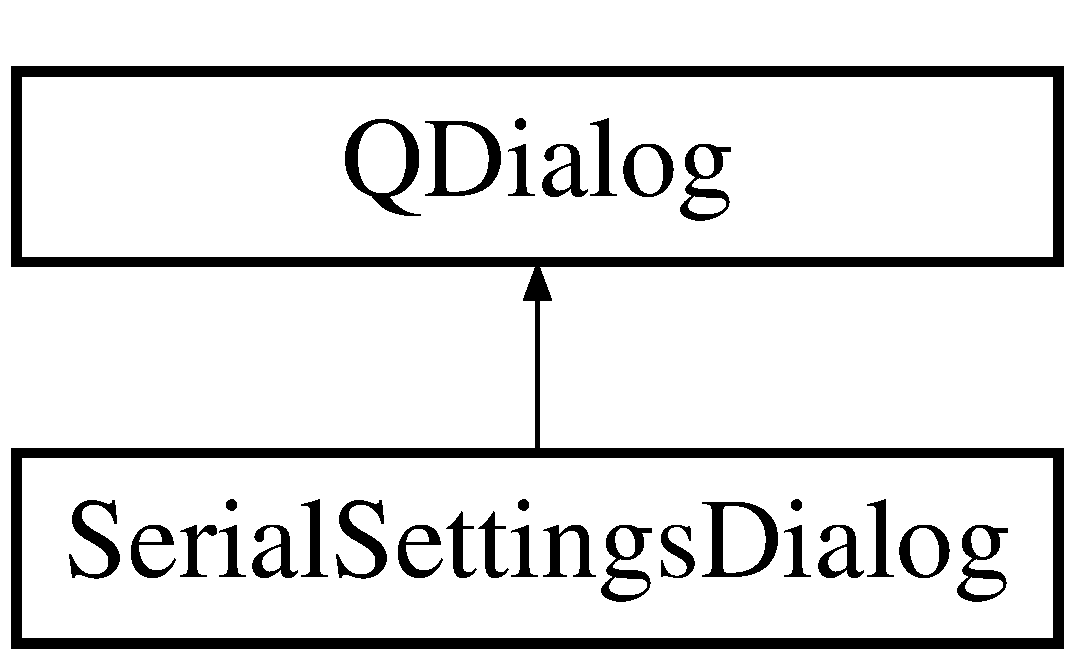
\includegraphics[height=2.000000cm]{classSerialSettingsDialog}
\end{center}
\end{figure}
\subsubsection*{Signals}
\begin{DoxyCompactItemize}
\item 
void \mbox{\hyperlink{classSerialSettingsDialog_a814c12a68be8eb01d2a5fe6fd9f6aaa7}{serial\+Setting\+Accepted}} (\mbox{\hyperlink{structComSettings}{Com\+Settings}} com\+Sett)
\end{DoxyCompactItemize}
\subsubsection*{Public Member Functions}
\begin{DoxyCompactItemize}
\item 
\mbox{\hyperlink{classSerialSettingsDialog_a5834dd80b40df594a5f93d664e1bba0a}{Serial\+Settings\+Dialog}} (Q\+Widget $\ast$parent=0)
\item 
\mbox{\hyperlink{classSerialSettingsDialog_ab8729269713f620c51862acc0f41f1fb}{Serial\+Settings\+Dialog}} (\mbox{\hyperlink{structComSettings}{Com\+Settings}} n\+Sett, Q\+Widget $\ast$parent=0)
\item 
\mbox{\hyperlink{classSerialSettingsDialog_a46a36a5ef33433be4a79c5d8b2b455ab}{$\sim$\+Serial\+Settings\+Dialog}} ()
\item 
\mbox{\hyperlink{structComSettings}{Com\+Settings}} \mbox{\hyperlink{classSerialSettingsDialog_a79327698eb7a95ab3b714cb4ccbc3599}{settings}} () const
\item 
void \mbox{\hyperlink{classSerialSettingsDialog_a0b31ad48fd2fe7fd9cce0c63eda3efb4}{set\+Settings}} (\mbox{\hyperlink{structComSettings}{Com\+Settings}} n\+Sett)
\end{DoxyCompactItemize}
\subsubsection*{Protected Member Functions}
\begin{DoxyCompactItemize}
\item 
void \mbox{\hyperlink{classSerialSettingsDialog_a1222ce503cf2d974869a674f186e4a11}{change\+Event}} (Q\+Event $\ast$event)
\end{DoxyCompactItemize}
\subsubsection*{Private Slots}
\begin{DoxyCompactItemize}
\item 
void \mbox{\hyperlink{classSerialSettingsDialog_a51bd57a094957fabb106e82b2a2fdcda}{show\+Port\+Info}} (int idx)
\item 
void \mbox{\hyperlink{classSerialSettingsDialog_a9172ba98481da3828d9825aa89fd2dd1}{apply}} ()
\item 
void \mbox{\hyperlink{classSerialSettingsDialog_ab0238e08301e18f365ab2239f129d868}{reject}} ()
\item 
void \mbox{\hyperlink{classSerialSettingsDialog_a3a731f098e834b3d17bc5ec0c2da64a5}{check\+Custom\+Baud\+Rate\+Policy}} (int idx)
\item 
void \mbox{\hyperlink{classSerialSettingsDialog_a784ef564d042f439ad94a2694a1ecbaf}{check\+Custom\+Device\+Path\+Policy}} (int idx)
\item 
void \mbox{\hyperlink{classSerialSettingsDialog_a4b813dfa2e8318f4d086e718b441d12e}{fill\+Ports\+Parameters}} ()
\item 
void \mbox{\hyperlink{classSerialSettingsDialog_a1b23a2eccc90ff6e9d50887e135584c8}{fill\+Ports\+Info}} ()
\item 
void \mbox{\hyperlink{classSerialSettingsDialog_ad41af1d1aba6bebce04969e141b914d4}{update\+Settings}} ()
\end{DoxyCompactItemize}
\subsubsection*{Private Attributes}
\begin{DoxyCompactItemize}
\item 
Ui\+::\+Serial\+Settings\+Dialog $\ast$ \mbox{\hyperlink{classSerialSettingsDialog_afc0d38e2824ab62ed7de597c97d012f7}{ui}}
\item 
bool \mbox{\hyperlink{classSerialSettingsDialog_ab87bf1b0042d98315035b07f4e340e0e}{accept\+On\+Deactilation\+En}}
\item 
\mbox{\hyperlink{structComSettings}{Com\+Settings}} \mbox{\hyperlink{classSerialSettingsDialog_ab24259a0385b292ff104425d97957482}{current\+Settings}}
\item 
Q\+Int\+Validator $\ast$ \mbox{\hyperlink{classSerialSettingsDialog_a0bd028bb39cf3db3b297a1899d3d835a}{int\+Validator}}
\end{DoxyCompactItemize}


\subsubsection{Constructor \& Destructor Documentation}
\mbox{\Hypertarget{classSerialSettingsDialog_a5834dd80b40df594a5f93d664e1bba0a}\label{classSerialSettingsDialog_a5834dd80b40df594a5f93d664e1bba0a}} 
\index{Serial\+Settings\+Dialog@{Serial\+Settings\+Dialog}!Serial\+Settings\+Dialog@{Serial\+Settings\+Dialog}}
\index{Serial\+Settings\+Dialog@{Serial\+Settings\+Dialog}!Serial\+Settings\+Dialog@{Serial\+Settings\+Dialog}}
{\footnotesize\ttfamily Serial\+Settings\+Dialog\+::\texorpdfstring{Serial\+Settings\+Dialog()}{SerialSettingsDialog()}\hspace{0.1cm}{\footnotesize\ttfamily [1/2]} (\begin{DoxyParamCaption}\item[{Q\+Widget $\ast$}]{parent = {\ttfamily 0} }\end{DoxyParamCaption})\hspace{0.3cm}{\ttfamily [explicit]}}

\mbox{\Hypertarget{classSerialSettingsDialog_ab8729269713f620c51862acc0f41f1fb}\label{classSerialSettingsDialog_ab8729269713f620c51862acc0f41f1fb}} 
\index{Serial\+Settings\+Dialog@{Serial\+Settings\+Dialog}!Serial\+Settings\+Dialog@{Serial\+Settings\+Dialog}}
\index{Serial\+Settings\+Dialog@{Serial\+Settings\+Dialog}!Serial\+Settings\+Dialog@{Serial\+Settings\+Dialog}}
{\footnotesize\ttfamily Serial\+Settings\+Dialog\+::\texorpdfstring{Serial\+Settings\+Dialog}{SerialSettingsDialog}\hspace{0.1cm}{\footnotesize\ttfamily [2/2]} (\begin{DoxyParamCaption}\item[{\mbox{\hyperlink{structComSettings}{Com\+Settings}}}]{n\+Sett,  }\item[{Q\+Widget $\ast$}]{parent = {\ttfamily 0} }\end{DoxyParamCaption})\hspace{0.3cm}{\ttfamily [explicit]}}

\mbox{\Hypertarget{classSerialSettingsDialog_a46a36a5ef33433be4a79c5d8b2b455ab}\label{classSerialSettingsDialog_a46a36a5ef33433be4a79c5d8b2b455ab}} 
\index{Serial\+Settings\+Dialog@{Serial\+Settings\+Dialog}!````~Serial\+Settings\+Dialog@{$\sim$\+Serial\+Settings\+Dialog}}
\index{````~Serial\+Settings\+Dialog@{$\sim$\+Serial\+Settings\+Dialog}!Serial\+Settings\+Dialog@{Serial\+Settings\+Dialog}}
{\footnotesize\ttfamily Serial\+Settings\+Dialog\+::\texorpdfstring{$\sim$\+Serial\+Settings\+Dialog}{~SerialSettingsDialog} (\begin{DoxyParamCaption}{ }\end{DoxyParamCaption})}



\subsubsection{Member Function Documentation}
\mbox{\Hypertarget{classSerialSettingsDialog_a9172ba98481da3828d9825aa89fd2dd1}\label{classSerialSettingsDialog_a9172ba98481da3828d9825aa89fd2dd1}} 
\index{Serial\+Settings\+Dialog@{Serial\+Settings\+Dialog}!apply@{apply}}
\index{apply@{apply}!Serial\+Settings\+Dialog@{Serial\+Settings\+Dialog}}
{\footnotesize\ttfamily void Serial\+Settings\+Dialog\+::\texorpdfstring{apply}{apply} (\begin{DoxyParamCaption}{ }\end{DoxyParamCaption})\hspace{0.3cm}{\ttfamily [private]}, {\ttfamily [slot]}}

\mbox{\Hypertarget{classSerialSettingsDialog_a1222ce503cf2d974869a674f186e4a11}\label{classSerialSettingsDialog_a1222ce503cf2d974869a674f186e4a11}} 
\index{Serial\+Settings\+Dialog@{Serial\+Settings\+Dialog}!change\+Event@{change\+Event}}
\index{change\+Event@{change\+Event}!Serial\+Settings\+Dialog@{Serial\+Settings\+Dialog}}
{\footnotesize\ttfamily void Serial\+Settings\+Dialog\+::\texorpdfstring{change\+Event}{changeEvent} (\begin{DoxyParamCaption}\item[{Q\+Event $\ast$}]{event }\end{DoxyParamCaption})\hspace{0.3cm}{\ttfamily [protected]}}

\mbox{\Hypertarget{classSerialSettingsDialog_a3a731f098e834b3d17bc5ec0c2da64a5}\label{classSerialSettingsDialog_a3a731f098e834b3d17bc5ec0c2da64a5}} 
\index{Serial\+Settings\+Dialog@{Serial\+Settings\+Dialog}!check\+Custom\+Baud\+Rate\+Policy@{check\+Custom\+Baud\+Rate\+Policy}}
\index{check\+Custom\+Baud\+Rate\+Policy@{check\+Custom\+Baud\+Rate\+Policy}!Serial\+Settings\+Dialog@{Serial\+Settings\+Dialog}}
{\footnotesize\ttfamily void Serial\+Settings\+Dialog\+::\texorpdfstring{check\+Custom\+Baud\+Rate\+Policy}{checkCustomBaudRatePolicy} (\begin{DoxyParamCaption}\item[{int}]{idx }\end{DoxyParamCaption})\hspace{0.3cm}{\ttfamily [private]}, {\ttfamily [slot]}}

\mbox{\Hypertarget{classSerialSettingsDialog_a784ef564d042f439ad94a2694a1ecbaf}\label{classSerialSettingsDialog_a784ef564d042f439ad94a2694a1ecbaf}} 
\index{Serial\+Settings\+Dialog@{Serial\+Settings\+Dialog}!check\+Custom\+Device\+Path\+Policy@{check\+Custom\+Device\+Path\+Policy}}
\index{check\+Custom\+Device\+Path\+Policy@{check\+Custom\+Device\+Path\+Policy}!Serial\+Settings\+Dialog@{Serial\+Settings\+Dialog}}
{\footnotesize\ttfamily void Serial\+Settings\+Dialog\+::\texorpdfstring{check\+Custom\+Device\+Path\+Policy}{checkCustomDevicePathPolicy} (\begin{DoxyParamCaption}\item[{int}]{idx }\end{DoxyParamCaption})\hspace{0.3cm}{\ttfamily [private]}, {\ttfamily [slot]}}

\mbox{\Hypertarget{classSerialSettingsDialog_a1b23a2eccc90ff6e9d50887e135584c8}\label{classSerialSettingsDialog_a1b23a2eccc90ff6e9d50887e135584c8}} 
\index{Serial\+Settings\+Dialog@{Serial\+Settings\+Dialog}!fill\+Ports\+Info@{fill\+Ports\+Info}}
\index{fill\+Ports\+Info@{fill\+Ports\+Info}!Serial\+Settings\+Dialog@{Serial\+Settings\+Dialog}}
{\footnotesize\ttfamily void Serial\+Settings\+Dialog\+::\texorpdfstring{fill\+Ports\+Info}{fillPortsInfo} (\begin{DoxyParamCaption}{ }\end{DoxyParamCaption})\hspace{0.3cm}{\ttfamily [private]}, {\ttfamily [slot]}}

\mbox{\Hypertarget{classSerialSettingsDialog_a4b813dfa2e8318f4d086e718b441d12e}\label{classSerialSettingsDialog_a4b813dfa2e8318f4d086e718b441d12e}} 
\index{Serial\+Settings\+Dialog@{Serial\+Settings\+Dialog}!fill\+Ports\+Parameters@{fill\+Ports\+Parameters}}
\index{fill\+Ports\+Parameters@{fill\+Ports\+Parameters}!Serial\+Settings\+Dialog@{Serial\+Settings\+Dialog}}
{\footnotesize\ttfamily void Serial\+Settings\+Dialog\+::\texorpdfstring{fill\+Ports\+Parameters}{fillPortsParameters} (\begin{DoxyParamCaption}{ }\end{DoxyParamCaption})\hspace{0.3cm}{\ttfamily [private]}, {\ttfamily [slot]}}

\mbox{\Hypertarget{classSerialSettingsDialog_ab0238e08301e18f365ab2239f129d868}\label{classSerialSettingsDialog_ab0238e08301e18f365ab2239f129d868}} 
\index{Serial\+Settings\+Dialog@{Serial\+Settings\+Dialog}!reject@{reject}}
\index{reject@{reject}!Serial\+Settings\+Dialog@{Serial\+Settings\+Dialog}}
{\footnotesize\ttfamily void Serial\+Settings\+Dialog\+::\texorpdfstring{reject}{reject} (\begin{DoxyParamCaption}{ }\end{DoxyParamCaption})\hspace{0.3cm}{\ttfamily [private]}, {\ttfamily [slot]}}

\mbox{\Hypertarget{classSerialSettingsDialog_a814c12a68be8eb01d2a5fe6fd9f6aaa7}\label{classSerialSettingsDialog_a814c12a68be8eb01d2a5fe6fd9f6aaa7}} 
\index{Serial\+Settings\+Dialog@{Serial\+Settings\+Dialog}!serial\+Setting\+Accepted@{serial\+Setting\+Accepted}}
\index{serial\+Setting\+Accepted@{serial\+Setting\+Accepted}!Serial\+Settings\+Dialog@{Serial\+Settings\+Dialog}}
{\footnotesize\ttfamily void Serial\+Settings\+Dialog\+::\texorpdfstring{serial\+Setting\+Accepted}{serialSettingAccepted} (\begin{DoxyParamCaption}\item[{\mbox{\hyperlink{structComSettings}{Com\+Settings}}}]{com\+Sett }\end{DoxyParamCaption})\hspace{0.3cm}{\ttfamily [signal]}}

\mbox{\Hypertarget{classSerialSettingsDialog_a0b31ad48fd2fe7fd9cce0c63eda3efb4}\label{classSerialSettingsDialog_a0b31ad48fd2fe7fd9cce0c63eda3efb4}} 
\index{Serial\+Settings\+Dialog@{Serial\+Settings\+Dialog}!set\+Settings@{set\+Settings}}
\index{set\+Settings@{set\+Settings}!Serial\+Settings\+Dialog@{Serial\+Settings\+Dialog}}
{\footnotesize\ttfamily void Serial\+Settings\+Dialog\+::\texorpdfstring{set\+Settings}{setSettings} (\begin{DoxyParamCaption}\item[{\mbox{\hyperlink{structComSettings}{Com\+Settings}}}]{n\+Sett }\end{DoxyParamCaption})}

\mbox{\Hypertarget{classSerialSettingsDialog_a79327698eb7a95ab3b714cb4ccbc3599}\label{classSerialSettingsDialog_a79327698eb7a95ab3b714cb4ccbc3599}} 
\index{Serial\+Settings\+Dialog@{Serial\+Settings\+Dialog}!settings@{settings}}
\index{settings@{settings}!Serial\+Settings\+Dialog@{Serial\+Settings\+Dialog}}
{\footnotesize\ttfamily \mbox{\hyperlink{structComSettings}{Com\+Settings}} Serial\+Settings\+Dialog\+::\texorpdfstring{settings}{settings} (\begin{DoxyParamCaption}{ }\end{DoxyParamCaption}) const}

\mbox{\Hypertarget{classSerialSettingsDialog_a51bd57a094957fabb106e82b2a2fdcda}\label{classSerialSettingsDialog_a51bd57a094957fabb106e82b2a2fdcda}} 
\index{Serial\+Settings\+Dialog@{Serial\+Settings\+Dialog}!show\+Port\+Info@{show\+Port\+Info}}
\index{show\+Port\+Info@{show\+Port\+Info}!Serial\+Settings\+Dialog@{Serial\+Settings\+Dialog}}
{\footnotesize\ttfamily void Serial\+Settings\+Dialog\+::\texorpdfstring{show\+Port\+Info}{showPortInfo} (\begin{DoxyParamCaption}\item[{int}]{idx }\end{DoxyParamCaption})\hspace{0.3cm}{\ttfamily [private]}, {\ttfamily [slot]}}

\mbox{\Hypertarget{classSerialSettingsDialog_ad41af1d1aba6bebce04969e141b914d4}\label{classSerialSettingsDialog_ad41af1d1aba6bebce04969e141b914d4}} 
\index{Serial\+Settings\+Dialog@{Serial\+Settings\+Dialog}!update\+Settings@{update\+Settings}}
\index{update\+Settings@{update\+Settings}!Serial\+Settings\+Dialog@{Serial\+Settings\+Dialog}}
{\footnotesize\ttfamily void Serial\+Settings\+Dialog\+::\texorpdfstring{update\+Settings}{updateSettings} (\begin{DoxyParamCaption}{ }\end{DoxyParamCaption})\hspace{0.3cm}{\ttfamily [private]}, {\ttfamily [slot]}}



\subsubsection{Member Data Documentation}
\mbox{\Hypertarget{classSerialSettingsDialog_ab87bf1b0042d98315035b07f4e340e0e}\label{classSerialSettingsDialog_ab87bf1b0042d98315035b07f4e340e0e}} 
\index{Serial\+Settings\+Dialog@{Serial\+Settings\+Dialog}!accept\+On\+Deactilation\+En@{accept\+On\+Deactilation\+En}}
\index{accept\+On\+Deactilation\+En@{accept\+On\+Deactilation\+En}!Serial\+Settings\+Dialog@{Serial\+Settings\+Dialog}}
{\footnotesize\ttfamily bool Serial\+Settings\+Dialog\+::\texorpdfstring{accept\+On\+Deactilation\+En}{acceptOnDeactilationEn}\hspace{0.3cm}{\ttfamily [private]}}

\mbox{\Hypertarget{classSerialSettingsDialog_ab24259a0385b292ff104425d97957482}\label{classSerialSettingsDialog_ab24259a0385b292ff104425d97957482}} 
\index{Serial\+Settings\+Dialog@{Serial\+Settings\+Dialog}!current\+Settings@{current\+Settings}}
\index{current\+Settings@{current\+Settings}!Serial\+Settings\+Dialog@{Serial\+Settings\+Dialog}}
{\footnotesize\ttfamily \mbox{\hyperlink{structComSettings}{Com\+Settings}} Serial\+Settings\+Dialog\+::\texorpdfstring{current\+Settings}{currentSettings}\hspace{0.3cm}{\ttfamily [private]}}

\mbox{\Hypertarget{classSerialSettingsDialog_a0bd028bb39cf3db3b297a1899d3d835a}\label{classSerialSettingsDialog_a0bd028bb39cf3db3b297a1899d3d835a}} 
\index{Serial\+Settings\+Dialog@{Serial\+Settings\+Dialog}!int\+Validator@{int\+Validator}}
\index{int\+Validator@{int\+Validator}!Serial\+Settings\+Dialog@{Serial\+Settings\+Dialog}}
{\footnotesize\ttfamily Q\+Int\+Validator$\ast$ Serial\+Settings\+Dialog\+::\texorpdfstring{int\+Validator}{intValidator}\hspace{0.3cm}{\ttfamily [private]}}


The documentation for this class was generated from the following files\+:\begin{DoxyCompactItemize}
\item 
\mbox{\hyperlink{serialsettingsdialog_8h}{serialsettingsdialog.\+h}}\item 
\mbox{\hyperlink{serialsettingsdialog_8cpp}{serialsettingsdialog.\+cpp}}\end{DoxyCompactItemize}
\newpage
\hypertarget{classSettingDialog}{}\subsection{Setting\+Dialog Class Reference}
\label{classSettingDialog}\index{Setting\+Dialog@{Setting\+Dialog}}


{\ttfamily \#include $<$headsettingdialog.\+h$>$}

Inheritance diagram for Setting\+Dialog\+:\begin{figure}[H]
\begin{center}
\leavevmode
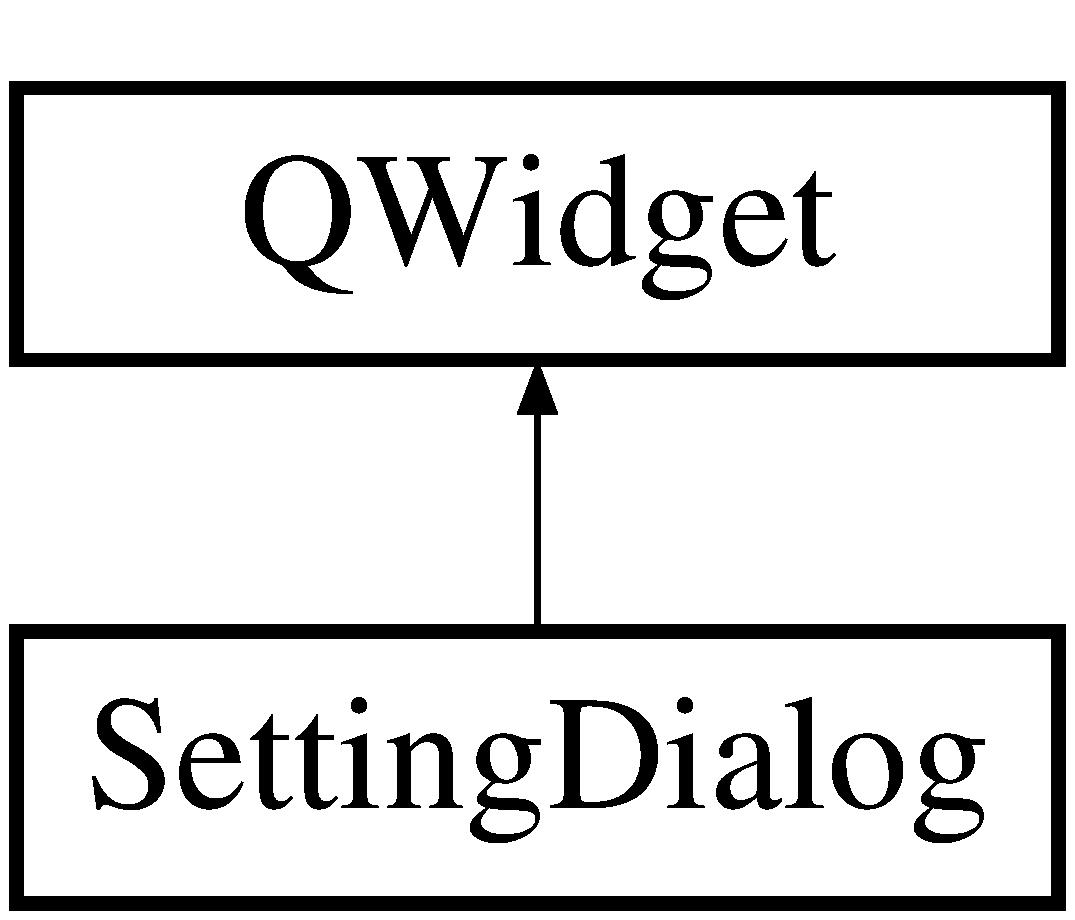
\includegraphics[height=2.000000cm]{classSettingDialog}
\end{center}
\end{figure}
\subsubsection*{Signals}
\begin{DoxyCompactItemize}
\item 
void \mbox{\hyperlink{classSettingDialog_abaf35d57bd061500e4d06c86bd9b7373}{accept}} (int \mbox{\hyperlink{classSettingDialog_a293670a08207442bb9ab04a734b70d33}{index}}, Q\+Byte\+Array h\+Param\+Arr)
\item 
void \mbox{\hyperlink{classSettingDialog_aaec8f3ce53ff211c0d2a3ebace6a4120}{change\+Number}} (int new\+Index)
\item 
void \mbox{\hyperlink{classSettingDialog_a88624538f0c2940ca17787bc797d695f}{send\+Command}} (int \mbox{\hyperlink{classSettingDialog_a293670a08207442bb9ab04a734b70d33}{index}}, Q\+Byte\+Array command)
\item 
void \mbox{\hyperlink{classSettingDialog_a3d2a5649a7c33127df571fef48c68744}{set\+Params\+To\+All}} (int \mbox{\hyperlink{classSettingDialog_a293670a08207442bb9ab04a734b70d33}{index}}, Q\+Byte\+Array h\+Param\+Arr)
\item 
void \mbox{\hyperlink{classSettingDialog_aa1a997bd3c53719f9d94a8c637d0a3e9}{color\+Changed}} (int \mbox{\hyperlink{classSettingDialog_a293670a08207442bb9ab04a734b70d33}{index}}, Q\+Color col)
\end{DoxyCompactItemize}
\subsubsection*{Public Member Functions}
\begin{DoxyCompactItemize}
\item 
\mbox{\hyperlink{classSettingDialog_ab7c9f7de85d73ca64b847ca3a0cd422a}{Setting\+Dialog}} (\mbox{\hyperlink{classHeadSetting}{Head\+Setting}} h\+Sttg, int \mbox{\hyperlink{classSettingDialog_a293670a08207442bb9ab04a734b70d33}{index}}=0, Q\+Widget $\ast$parent=0)
\item 
\mbox{\hyperlink{classSettingDialog_a9bfa278550d23df3f5e944989b0b0f54}{$\sim$\+Setting\+Dialog}} ()
\item 
void \mbox{\hyperlink{classSettingDialog_a43114394546e14f2a5c140591708b53d}{set\+Registers}} (\mbox{\hyperlink{classRegister}{Register}} $\ast$reg)
\item 
void \mbox{\hyperlink{classSettingDialog_a3ab742273bba41f566e2ec5e23e15adf}{set\+Head\+Params}} (int \mbox{\hyperlink{classSettingDialog_a293670a08207442bb9ab04a734b70d33}{index}}=0, bool disconnect=true)
\item 
void \mbox{\hyperlink{classSettingDialog_a25e9a36fc58d6cc9ae3fa63ff323d139}{set\+Head\+Params}} (\mbox{\hyperlink{classHeadSetting}{Head\+Setting}} h\+Sttg, int \mbox{\hyperlink{classSettingDialog_a293670a08207442bb9ab04a734b70d33}{index}}=0, bool disconnect=true)
\item 
void \mbox{\hyperlink{classSettingDialog_a47c392fce9b4379ee287f94ee13add91}{set\+Icon\+Folder}} (Q\+String path)
\end{DoxyCompactItemize}
\subsubsection*{Protected Member Functions}
\begin{DoxyCompactItemize}
\item 
bool \mbox{\hyperlink{classSettingDialog_a8946ea3396791c3bfdb0af9294432456}{event}} (Q\+Event $\ast$e)
\item 
bool \mbox{\hyperlink{classSettingDialog_aced29131c09a6a91867bd3d6b05f01dc}{event\+Filter}} (Q\+Object $\ast$watched, Q\+Event $\ast$\mbox{\hyperlink{classSettingDialog_a8946ea3396791c3bfdb0af9294432456}{event}})
\item 
void \mbox{\hyperlink{classSettingDialog_aaed08f2ad87702c7d6ff0a4a5df7e1e7}{show\+Event}} (Q\+Show\+Event $\ast$ev)
\item 
void \mbox{\hyperlink{classSettingDialog_a7aa0c7f2703bd6d208570eb7ed98e47b}{change\+Event}} (Q\+Event $\ast$\mbox{\hyperlink{classSettingDialog_a8946ea3396791c3bfdb0af9294432456}{event}})
\end{DoxyCompactItemize}
\subsubsection*{Private Slots}
\begin{DoxyCompactItemize}
\item 
void \mbox{\hyperlink{classSettingDialog_ac5caf772c1ad7d7607a164ad7f6fe647}{accept}} ()
\item 
void \mbox{\hyperlink{classSettingDialog_aa2d0391c28612987805722038013f5a9}{reject}} ()
\item 
void \mbox{\hyperlink{classSettingDialog_a586eff422c5c347ee5ff3ffe71b5ba97}{p\+Button\+Inc\+Clkd}} ()
\item 
void \mbox{\hyperlink{classSettingDialog_a87b4aca2d528b1b8e943983efc9d9506}{p\+Button\+Dec\+Clkd}} ()
\item 
void \mbox{\hyperlink{classSettingDialog_acd1bbe0b354633f39e4f0a15468098ad}{connect\+All}} ()
\item 
void \mbox{\hyperlink{classSettingDialog_a5d520fb11c481f648ed061cd700916fa}{disconnect\+All}} ()
\item 
void \mbox{\hyperlink{classSettingDialog_a01d7341608bd80021abd1a5892fdb131}{event\+Filter\+Setup}} ()
\item 
void \mbox{\hyperlink{classSettingDialog_a14896cba93080b0784380651579d809c}{temperature\+Sensore\+Changed}} (bool temp\+Sens)
\item 
void \mbox{\hyperlink{classSettingDialog_a57173bd31c0554d31571332ceb175b3d}{on\+\_\+tool\+Button\+Plast\+\_\+clicked}} ()
\item 
void \mbox{\hyperlink{classSettingDialog_a28734c990957727acebddabbe01fa442}{on\+\_\+tool\+Button\+F\+L\+\_\+clicked}} ()
\item 
void \mbox{\hyperlink{classSettingDialog_a2622da82b9284689d035a96c2c3642f5}{on\+\_\+tool\+Button\+Move\+Rear\+\_\+clicked}} ()
\item 
void \mbox{\hyperlink{classSettingDialog_adf5bed0777bbaa36f25b9280528cf342}{on\+\_\+tool\+Button\+F\+L\+\_\+\+S\+Qup\+\_\+clicked}} ()
\item 
void \mbox{\hyperlink{classSettingDialog_a40bed1f6bde134fabcd9b39e4498cffb}{on\+\_\+tool\+Button\+Move\+Front\+\_\+clicked}} ()
\item 
void \mbox{\hyperlink{classSettingDialog_a44def5923853f2e47dc2ad8247a62227}{on\+\_\+tool\+Button\+M\+T\+P\+Move\+\_\+clicked}} ()
\item 
void \mbox{\hyperlink{classSettingDialog_a4c777f59dac2be7467f61d171b937a9f}{on\+\_\+tool\+Button\+S\+Q\+\_\+clicked}} ()
\item 
void \mbox{\hyperlink{classSettingDialog_a9fd57e56c1364cb5107b314bec9d414d}{on\+\_\+tool\+Button\+Move\+Test\+\_\+clicked}} ()
\item 
void \mbox{\hyperlink{classSettingDialog_a0745d27f5e4a4d24b0722123bc06d25e}{on\+\_\+tool\+Button\+Pressure\+\_\+clicked}} ()
\item 
void \mbox{\hyperlink{classSettingDialog_ac1ac55a6bfd2730cad20f4bcc2805049}{on\+\_\+tool\+Button\+Hold\+On\+\_\+clicked}} ()
\item 
void \mbox{\hyperlink{classSettingDialog_a40f0ebcd38f004373ce6037a47f55da7}{on\+\_\+tool\+Button\+F\+L\+\_\+\+S\+Q\+\_\+clicked}} ()
\item 
void \mbox{\hyperlink{classSettingDialog_a24027ff6daaf9b3537de48ec915ad428}{on\+\_\+tool\+Button\+Step\+Back\+\_\+clicked}} ()
\item 
void \mbox{\hyperlink{classSettingDialog_ae6edcd6a2151ec8402904fd33cbd1a95}{on\+\_\+tool\+Button\+Index\+Here\+\_\+clicked}} ()
\item 
void \mbox{\hyperlink{classSettingDialog_aa4c4eae09fcec8ad3a2bb8615e314e39}{on\+\_\+tool\+Button\+Ink\+Color\+\_\+clicked}} ()
\item 
void \mbox{\hyperlink{classSettingDialog_a08f91f306b9e5fbe3f24dea1bc8b7152}{on\+\_\+tool\+Button\+Pressure\+Air\+\_\+clicked}} ()
\item 
void \mbox{\hyperlink{classSettingDialog_a0fd7b8d8b9d06ff10dd9136e699cb5f0}{on\+\_\+p\+Button\+Head\+On\+Off\+\_\+clicked}} ()
\item 
void \mbox{\hyperlink{classSettingDialog_a2eb481548395d6d2459456076678bcf1}{on\+\_\+tool\+Button\+Quartz\+Preheat\+\_\+clicked}} ()
\item 
void \mbox{\hyperlink{classSettingDialog_a4030986a71c3245c64458117b358f5cc}{on\+\_\+tool\+Button\+Quartz\+Test\+\_\+clicked}} ()
\item 
void \mbox{\hyperlink{classSettingDialog_a7c13d35ab90a6bc7e77a7eb02e90df82}{on\+\_\+tool\+Button\+Quartz\+Step\+Back\+\_\+clicked}} ()
\item 
void \mbox{\hyperlink{classSettingDialog_af6128bbe3289b7033e27d0e2d439e24b}{on\+\_\+tool\+Button\+Quartz\+Warming\+\_\+clicked}} ()
\item 
void \mbox{\hyperlink{classSettingDialog_a991a3f7add65873f5e790dbc5b2d98f7}{on\+\_\+push\+Button\+Copy\+To\+All\+\_\+clicked}} ()
\item 
void \mbox{\hyperlink{classSettingDialog_a1e0138fa136b0723568b8ebed97fc6f6}{tab\+Widget\+\_\+current\+Changed}} (int \mbox{\hyperlink{classSettingDialog_a293670a08207442bb9ab04a734b70d33}{index}})
\item 
void \mbox{\hyperlink{classSettingDialog_aa6602067bd18c4e6e845d0c217380120}{spin\+Box\+Rear\+Speed\+\_\+value\+Changed}} (double arg1)
\item 
void \mbox{\hyperlink{classSettingDialog_a8a2f78f4b1107c94a07880c93ecaebc4}{d\+Spin\+Box\+Rear\+Range\+\_\+value\+Changed}} (double arg1)
\item 
void \mbox{\hyperlink{classSettingDialog_a02039d7e4a584da46e7bf658b8ed78a7}{spin\+Box\+Front\+Speed\+\_\+value\+Changed}} (double arg1)
\item 
void \mbox{\hyperlink{classSettingDialog_a2943dbf41bfa2b9cee5ad661447ca9be}{d\+Spin\+Box\+Front\+Range\+\_\+value\+Changed}} (double arg1)
\item 
void \mbox{\hyperlink{classSettingDialog_a6cd6886cf912cfb5275754183334e70f}{spin\+Box\+Strok\+Count\+\_\+value\+Changed}} (double arg1)
\item 
void \mbox{\hyperlink{classSettingDialog_abe2d0f0bf0ea4c12cdd18b4c63e18ef2}{spin\+Box\+S\+B\+Strok\+Count\+\_\+value\+Changed}} (double arg1)
\item 
void \mbox{\hyperlink{classSettingDialog_a14fb25d61fdf8e847806ae6ae0143979}{d\+Spin\+Box\+Heat\+Time1\+I\+R\+\_\+value\+Changed}} (double arg1)
\item 
void \mbox{\hyperlink{classSettingDialog_ac43003a00b40d40c1d8518429234d52a}{d\+Spin\+Box\+Heat\+Time2\+I\+R\+\_\+value\+Changed}} (double arg1)
\item 
void \mbox{\hyperlink{classSettingDialog_a9ca34f0f0587dc274c346a0198e69332}{d\+Spin\+Box\+Drying\+Range\+I\+R\+\_\+value\+Changed}} (double arg1)
\item 
void \mbox{\hyperlink{classSettingDialog_a2ba1d0392bf7d998803541765f2114d7}{d\+Spin\+Box\+Fl\+Dwell\+Time\+\_\+value\+Changed}} (double arg1)
\item 
void \mbox{\hyperlink{classSettingDialog_a37e06665f728195a910d80f586cb8932}{d\+Spin\+Box\+Sq\+Dwell\+Time\+\_\+value\+Changed}} (double arg1)
\item 
void \mbox{\hyperlink{classSettingDialog_a2b0e2cfbda5f92f47197fd154e4a7641}{d\+Spin\+Box\+Heat\+Time1\+Q\+\_\+value\+Changed}} (double arg1)
\item 
void \mbox{\hyperlink{classSettingDialog_ac3915bcd030a25082dab75845291c1e7}{d\+Spin\+Box\+Heat\+Time2\+Q\+\_\+value\+Changed}} (double arg1)
\item 
void \mbox{\hyperlink{classSettingDialog_a79c8072c55146ad38a739567b2233c1f}{spin\+Box\+Dry\+Power\+Q\+\_\+value\+Changed}} (double arg1)
\item 
void \mbox{\hyperlink{classSettingDialog_a94dab1fe735e3991220956b64c21219b}{d\+Spin\+Box\+Stepback\+Dry\+Time\+Q\+\_\+value\+Changed}} (double arg1)
\item 
void \mbox{\hyperlink{classSettingDialog_a373951de775a1b220c6d7d9abd59f76c}{d\+Spin\+Box\+Temperature\+Set\+Q\+\_\+value\+Changed}} (double arg1)
\item 
void \mbox{\hyperlink{classSettingDialog_aa6079278861db915fe4a4d18b5008a6e}{d\+Spin\+Box\+Dry\+Time\+Q\+\_\+value\+Changed}} (double arg1)
\item 
void \mbox{\hyperlink{classSettingDialog_a453eecb0650ad29e6d14fb641ef79697}{spin\+Box\+Standby\+Power\+Q\+\_\+value\+Changed}} (double arg1)
\item 
void \mbox{\hyperlink{classSettingDialog_af40ee40d8aff8550e5ffe2ccdac384ae}{d\+Spin\+Box\+Standby\+Time\+Q\+\_\+value\+Changed}} (double arg1)
\item 
void \mbox{\hyperlink{classSettingDialog_af6f257e19ab8d0bc8f724c217c5039af}{d\+Spin\+Box\+Warm\+Flash\+Time\+Q\+\_\+value\+Changed}} (double arg1)
\item 
void \mbox{\hyperlink{classSettingDialog_a0670d5bdf419372d7c5e314b45064a85}{r\+Button\+Time1\+\_\+clicked}} ()
\end{DoxyCompactItemize}
\subsubsection*{Private Attributes}
\begin{DoxyCompactItemize}
\item 
Ui\+::\+Setting\+Dialog $\ast$ \mbox{\hyperlink{classSettingDialog_a445c68adc5c9f920537e4637f9c7e55b}{ui}}
\item 
bool \mbox{\hyperlink{classSettingDialog_a92ac83de20616f1f67f369dec0afe5f0}{with\+Temperature\+Sensor}}
\item 
int \mbox{\hyperlink{classSettingDialog_a293670a08207442bb9ab04a734b70d33}{index}}
\item 
bool \mbox{\hyperlink{classSettingDialog_a76fcfae71a48ee3d0ab4d7a28f850d1a}{accept\+On\+Deactilation\+En}}
\item 
bool \mbox{\hyperlink{classSettingDialog_a5091b6757e8f987f4bdf5de856b694f6}{accept\+Enable}}
\item 
\mbox{\hyperlink{classHeadSetting}{Head\+Setting}} \mbox{\hyperlink{classSettingDialog_ae53d3ff786571f3291668e3d90ad16cb}{head\+Settings}}
\item 
\mbox{\hyperlink{classRegister}{Register}} $\ast$ \mbox{\hyperlink{classSettingDialog_a66c450ef93bc3346d5b2fa08eb58d48f}{registers}}
\end{DoxyCompactItemize}


\subsubsection{Constructor \& Destructor Documentation}
\mbox{\Hypertarget{classSettingDialog_ab7c9f7de85d73ca64b847ca3a0cd422a}\label{classSettingDialog_ab7c9f7de85d73ca64b847ca3a0cd422a}} 
\index{Setting\+Dialog@{Setting\+Dialog}!Setting\+Dialog@{Setting\+Dialog}}
\index{Setting\+Dialog@{Setting\+Dialog}!Setting\+Dialog@{Setting\+Dialog}}
{\footnotesize\ttfamily Setting\+Dialog\+::\texorpdfstring{Setting\+Dialog}{SettingDialog} (\begin{DoxyParamCaption}\item[{\mbox{\hyperlink{classHeadSetting}{Head\+Setting}}}]{h\+Sttg,  }\item[{int}]{index = {\ttfamily 0},  }\item[{Q\+Widget $\ast$}]{parent = {\ttfamily 0} }\end{DoxyParamCaption})\hspace{0.3cm}{\ttfamily [explicit]}} - class constructor. At constructor fields of dialog fill with parameters given at \textit{hSttg} and call \hyperlink{classSettingDialog_a01d7341608bd80021abd1a5892fdb131}{event\+Filter\+Setup}(...) function.

\mbox{\Hypertarget{classSettingDialog_a9bfa278550d23df3f5e944989b0b0f54}\label{classSettingDialog_a9bfa278550d23df3f5e944989b0b0f54}} 
\index{Setting\+Dialog@{Setting\+Dialog}!````~Setting\+Dialog@{$\sim$\+Setting\+Dialog}}
\index{````~Setting\+Dialog@{$\sim$\+Setting\+Dialog}!Setting\+Dialog@{Setting\+Dialog}}
{\footnotesize\ttfamily Setting\+Dialog\+::\texorpdfstring{$\sim$\+Setting\+Dialog}{~SettingDialog} (\begin{DoxyParamCaption}{ }\end{DoxyParamCaption})} - standard destructor.



\subsubsection{Member Function Documentation}
\mbox{\Hypertarget{classSettingDialog_abaf35d57bd061500e4d06c86bd9b7373}\label{classSettingDialog_abaf35d57bd061500e4d06c86bd9b7373}} 
\index{Setting\+Dialog@{Setting\+Dialog}!accept@{accept}}
\index{accept@{accept}!Setting\+Dialog@{Setting\+Dialog}}
{\footnotesize\ttfamily void Setting\+Dialog\+::\texorpdfstring{accept}{accept}\hspace{0.1cm} (\begin{DoxyParamCaption}\item[{int}]{index,  }\item[{Q\+Byte\+Array}]{h\+Param\+Arr }\end{DoxyParamCaption})\hspace{0.3cm}{\ttfamily [signal]}} - signal which emitted by \hyperlink{classSettingDialog_ac5caf772c1ad7d7607a164ad7f6fe647}{accept}(...) function and handled in parent object. Parameter \textit{index} contain information about head number, and \textit{h\+Param\+Arr} contain all head parameters. Parameters are save to hard drive at parent object.

\mbox{\Hypertarget{classSettingDialog_ac5caf772c1ad7d7607a164ad7f6fe647}\label{classSettingDialog_ac5caf772c1ad7d7607a164ad7f6fe647}} 
\index{Setting\+Dialog@{Setting\+Dialog}!accept@{accept}}
\index{accept@{accept}!Setting\+Dialog@{Setting\+Dialog}}
{\footnotesize\ttfamily void Setting\+Dialog\+::\texorpdfstring{accept}{accept}\hspace{0.1cm} (\begin{DoxyParamCaption}{ }\end{DoxyParamCaption})\hspace{0.3cm}{\ttfamily [private]}, {\ttfamily [slot]}} - function to collect head parameters, put them to appropriate places at array and emit \hyperlink{classSettingDialog_abaf35d57bd061500e4d06c86bd9b7373}{accept}(...) signal.

\mbox{\Hypertarget{classSettingDialog_a7aa0c7f2703bd6d208570eb7ed98e47b}\label{classSettingDialog_a7aa0c7f2703bd6d208570eb7ed98e47b}} 
\index{Setting\+Dialog@{Setting\+Dialog}!change\+Event@{change\+Event}}
\index{change\+Event@{change\+Event}!Setting\+Dialog@{Setting\+Dialog}}
{\footnotesize\ttfamily void Setting\+Dialog\+::\texorpdfstring{change\+Event}{changeEvent} (\begin{DoxyParamCaption}\item[{Q\+Event $\ast$}]{event }\end{DoxyParamCaption})\hspace{0.3cm}{\ttfamily [protected]}}- reimplementation of default event of Q\+Dialog to enable user interface translation. Function called automatically.

\mbox{\Hypertarget{classSettingDialog_aaec8f3ce53ff211c0d2a3ebace6a4120}\label{classSettingDialog_aaec8f3ce53ff211c0d2a3ebace6a4120}} 
\index{Setting\+Dialog@{Setting\+Dialog}!change\+Number@{change\+Number}}
\index{change\+Number@{change\+Number}!Setting\+Dialog@{Setting\+Dialog}}
{\footnotesize\ttfamily void Setting\+Dialog\+::\texorpdfstring{change\+Number}{changeNumber} (\begin{DoxyParamCaption}\item[{int}]{new\+Index }\end{DoxyParamCaption})\hspace{0.3cm}{\ttfamily [signal]}} - signal which handle at parent object and used for fast change of head number. Signal emits by \hyperlink{classSettingDialog_a586eff422c5c347ee5ff3ffe71b5ba97}{p\+Button\+Inc\+Clkd}(...) and \hyperlink{classSettingDialog_a87b4aca2d528b1b8e943983efc9d9506}{p\+Button\+Dec\+Clkd}(...) functions with appropriate value of parameter.

\mbox{\Hypertarget{classSettingDialog_aa1a997bd3c53719f9d94a8c637d0a3e9}\label{classSettingDialog_aa1a997bd3c53719f9d94a8c637d0a3e9}} 
\index{Setting\+Dialog@{Setting\+Dialog}!color\+Changed@{color\+Changed}}
\index{color\+Changed@{color\+Changed}!Setting\+Dialog@{Setting\+Dialog}}
{\footnotesize\ttfamily void Setting\+Dialog\+::\texorpdfstring{color\+Changed}{colorChanged} (\begin{DoxyParamCaption}\item[{int}]{index,  }\item[{Q\+Color}]{col }\end{DoxyParamCaption})\hspace{0.3cm}{\ttfamily [signal]}} - signal which emits by \hyperlink{classSettingDialog_aa4c4eae09fcec8ad3a2bb8615e314e39}{on\+\_\+tool\+Button\+Ink\+Color\+\_\+clicked}(...) function. Signal contain information about rag color on head.

\mbox{\Hypertarget{classSettingDialog_acd1bbe0b354633f39e4f0a15468098ad}\label{classSettingDialog_acd1bbe0b354633f39e4f0a15468098ad}} 
\index{Setting\+Dialog@{Setting\+Dialog}!connect\+All@{connect\+All}}
\index{connect\+All@{connect\+All}!Setting\+Dialog@{Setting\+Dialog}}
{\footnotesize\ttfamily void Setting\+Dialog\+::\texorpdfstring{connect\+All}{connectAll} (\begin{DoxyParamCaption}{ }\end{DoxyParamCaption})\hspace{0.3cm}{\ttfamily [private]}, {\ttfamily [slot]}} - function to connect all fields of dialog to appropriate functions.

\mbox{\Hypertarget{classSettingDialog_a5d520fb11c481f648ed061cd700916fa}\label{classSettingDialog_a5d520fb11c481f648ed061cd700916fa}} 
\index{Setting\+Dialog@{Setting\+Dialog}!disconnect\+All@{disconnect\+All}}
\index{disconnect\+All@{disconnect\+All}!Setting\+Dialog@{Setting\+Dialog}}
{\footnotesize\ttfamily void Setting\+Dialog\+::\texorpdfstring{disconnect\+All}{disconnectAll} (\begin{DoxyParamCaption}{ }\end{DoxyParamCaption})\hspace{0.3cm}{\ttfamily [private]}, {\ttfamily [slot]}} - function to disconnect all fields of dialog to appropriate functions.

\begin{center}	\line(1,0){450} \end{center}
All functions in next block used to send parameters to master PCB to configure machine. \\
Functions used to get values from fields with head parameters, gather them into byte array and emit \hyperlink{classSettingDialog_a88624538f0c2940ca17787bc797d695f}{send\+Command}(...) signal with appropriate data.

\begin{DoxyCompactItemize}
\item\mbox{\Hypertarget{classSettingDialog_a9ca34f0f0587dc274c346a0198e69332}\label{classSettingDialog_a9ca34f0f0587dc274c346a0198e69332}} 
\index{Setting\+Dialog@{Setting\+Dialog}!d\+Spin\+Box\+Drying\+Range\+I\+R\+\_\+value\+Changed@{d\+Spin\+Box\+Drying\+Range\+I\+R\+\_\+value\+Changed}}
\index{d\+Spin\+Box\+Drying\+Range\+I\+R\+\_\+value\+Changed@{d\+Spin\+Box\+Drying\+Range\+I\+R\+\_\+value\+Changed}!Setting\+Dialog@{Setting\+Dialog}}
{\footnotesize\ttfamily void Setting\+Dialog\+::\texorpdfstring{d\+Spin\+Box\+Drying\+Range\+I\+R\+\_\+value\+Changed}{dSpinBoxDryingRangeIR\_valueChanged} (\begin{DoxyParamCaption}\item[{double}]{arg1 }\end{DoxyParamCaption})\hspace{0.3cm}{\ttfamily [private]}, {\ttfamily [slot]}}

\item\mbox{\Hypertarget{classSettingDialog_aa6079278861db915fe4a4d18b5008a6e}\label{classSettingDialog_aa6079278861db915fe4a4d18b5008a6e}} 
\index{Setting\+Dialog@{Setting\+Dialog}!d\+Spin\+Box\+Dry\+Time\+Q\+\_\+value\+Changed@{d\+Spin\+Box\+Dry\+Time\+Q\+\_\+value\+Changed}}
\index{d\+Spin\+Box\+Dry\+Time\+Q\+\_\+value\+Changed@{d\+Spin\+Box\+Dry\+Time\+Q\+\_\+value\+Changed}!Setting\+Dialog@{Setting\+Dialog}}
{\footnotesize\ttfamily void Setting\+Dialog\+::\texorpdfstring{d\+Spin\+Box\+Dry\+Time\+Q\+\_\+value\+Changed}{dSpinBoxDryTimeQ\_valueChanged} (\begin{DoxyParamCaption}\item[{double}]{arg1 }\end{DoxyParamCaption})\hspace{0.3cm}{\ttfamily [private]}, {\ttfamily [slot]}}

\item\mbox{\Hypertarget{classSettingDialog_a2ba1d0392bf7d998803541765f2114d7}\label{classSettingDialog_a2ba1d0392bf7d998803541765f2114d7}} 
\index{Setting\+Dialog@{Setting\+Dialog}!d\+Spin\+Box\+Fl\+Dwell\+Time\+\_\+value\+Changed@{d\+Spin\+Box\+Fl\+Dwell\+Time\+\_\+value\+Changed}}
\index{d\+Spin\+Box\+Fl\+Dwell\+Time\+\_\+value\+Changed@{d\+Spin\+Box\+Fl\+Dwell\+Time\+\_\+value\+Changed}!Setting\+Dialog@{Setting\+Dialog}}
{\footnotesize\ttfamily void Setting\+Dialog\+::\texorpdfstring{d\+Spin\+Box\+Fl\+Dwell\+Time\+\_\+value\+Changed}{dSpinBoxFlDwellTime\_valueChanged} (\begin{DoxyParamCaption}\item[{double}]{arg1 }\end{DoxyParamCaption})\hspace{0.3cm}{\ttfamily [private]}, {\ttfamily [slot]}}

\item\mbox{\Hypertarget{classSettingDialog_a2943dbf41bfa2b9cee5ad661447ca9be}\label{classSettingDialog_a2943dbf41bfa2b9cee5ad661447ca9be}} 
\index{Setting\+Dialog@{Setting\+Dialog}!d\+Spin\+Box\+Front\+Range\+\_\+value\+Changed@{d\+Spin\+Box\+Front\+Range\+\_\+value\+Changed}}
\index{d\+Spin\+Box\+Front\+Range\+\_\+value\+Changed@{d\+Spin\+Box\+Front\+Range\+\_\+value\+Changed}!Setting\+Dialog@{Setting\+Dialog}}
{\footnotesize\ttfamily void Setting\+Dialog\+::\texorpdfstring{d\+Spin\+Box\+Front\+Range\+\_\+value\+Changed}{dSpinBoxFrontRange\_valueChanged} (\begin{DoxyParamCaption}\item[{double}]{arg1 }\end{DoxyParamCaption})\hspace{0.3cm}{\ttfamily [private]}, {\ttfamily [slot]}}

\item\mbox{\Hypertarget{classSettingDialog_a14fb25d61fdf8e847806ae6ae0143979}\label{classSettingDialog_a14fb25d61fdf8e847806ae6ae0143979}} 
\index{Setting\+Dialog@{Setting\+Dialog}!d\+Spin\+Box\+Heat\+Time1\+I\+R\+\_\+value\+Changed@{d\+Spin\+Box\+Heat\+Time1\+I\+R\+\_\+value\+Changed}}
\index{d\+Spin\+Box\+Heat\+Time1\+I\+R\+\_\+value\+Changed@{d\+Spin\+Box\+Heat\+Time1\+I\+R\+\_\+value\+Changed}!Setting\+Dialog@{Setting\+Dialog}}
{\footnotesize\ttfamily void Setting\+Dialog\+::\texorpdfstring{d\+Spin\+Box\+Heat\+Time1\+I\+R\+\_\+value\+Changed}{dSpinBoxHeatTime1IR\_valueChanged} (\begin{DoxyParamCaption}\item[{double}]{arg1 }\end{DoxyParamCaption})\hspace{0.3cm}{\ttfamily [private]}, {\ttfamily [slot]}}

\item\mbox{\Hypertarget{classSettingDialog_a2b0e2cfbda5f92f47197fd154e4a7641}\label{classSettingDialog_a2b0e2cfbda5f92f47197fd154e4a7641}} 
\index{Setting\+Dialog@{Setting\+Dialog}!d\+Spin\+Box\+Heat\+Time1\+Q\+\_\+value\+Changed@{d\+Spin\+Box\+Heat\+Time1\+Q\+\_\+value\+Changed}}
\index{d\+Spin\+Box\+Heat\+Time1\+Q\+\_\+value\+Changed@{d\+Spin\+Box\+Heat\+Time1\+Q\+\_\+value\+Changed}!Setting\+Dialog@{Setting\+Dialog}}
{\footnotesize\ttfamily void Setting\+Dialog\+::\texorpdfstring{d\+Spin\+Box\+Heat\+Time1\+Q\+\_\+value\+Changed}{dSpinBoxHeatTime1Q\_valueChanged} (\begin{DoxyParamCaption}\item[{double}]{arg1 }\end{DoxyParamCaption})\hspace{0.3cm}{\ttfamily [private]}, {\ttfamily [slot]}}

\item\mbox{\Hypertarget{classSettingDialog_ac43003a00b40d40c1d8518429234d52a}\label{classSettingDialog_ac43003a00b40d40c1d8518429234d52a}} 
\index{Setting\+Dialog@{Setting\+Dialog}!d\+Spin\+Box\+Heat\+Time2\+I\+R\+\_\+value\+Changed@{d\+Spin\+Box\+Heat\+Time2\+I\+R\+\_\+value\+Changed}}
\index{d\+Spin\+Box\+Heat\+Time2\+I\+R\+\_\+value\+Changed@{d\+Spin\+Box\+Heat\+Time2\+I\+R\+\_\+value\+Changed}!Setting\+Dialog@{Setting\+Dialog}}
{\footnotesize\ttfamily void Setting\+Dialog\+::\texorpdfstring{d\+Spin\+Box\+Heat\+Time2\+I\+R\+\_\+value\+Changed}{dSpinBoxHeatTime2IR\_valueChanged} (\begin{DoxyParamCaption}\item[{double}]{arg1 }\end{DoxyParamCaption})\hspace{0.3cm}{\ttfamily [private]}, {\ttfamily [slot]}}

\item\mbox{\Hypertarget{classSettingDialog_ac3915bcd030a25082dab75845291c1e7}\label{classSettingDialog_ac3915bcd030a25082dab75845291c1e7}} 
\index{Setting\+Dialog@{Setting\+Dialog}!d\+Spin\+Box\+Heat\+Time2\+Q\+\_\+value\+Changed@{d\+Spin\+Box\+Heat\+Time2\+Q\+\_\+value\+Changed}}
\index{d\+Spin\+Box\+Heat\+Time2\+Q\+\_\+value\+Changed@{d\+Spin\+Box\+Heat\+Time2\+Q\+\_\+value\+Changed}!Setting\+Dialog@{Setting\+Dialog}}
{\footnotesize\ttfamily void Setting\+Dialog\+::\texorpdfstring{d\+Spin\+Box\+Heat\+Time2\+Q\+\_\+value\+Changed}{dSpinBoxHeatTime2Q\_valueChanged} (\begin{DoxyParamCaption}\item[{double}]{arg1 }\end{DoxyParamCaption})\hspace{0.3cm}{\ttfamily [private]}, {\ttfamily [slot]}}

\item\mbox{\Hypertarget{classSettingDialog_a8a2f78f4b1107c94a07880c93ecaebc4}\label{classSettingDialog_a8a2f78f4b1107c94a07880c93ecaebc4}} 
\index{Setting\+Dialog@{Setting\+Dialog}!d\+Spin\+Box\+Rear\+Range\+\_\+value\+Changed@{d\+Spin\+Box\+Rear\+Range\+\_\+value\+Changed}}
\index{d\+Spin\+Box\+Rear\+Range\+\_\+value\+Changed@{d\+Spin\+Box\+Rear\+Range\+\_\+value\+Changed}!Setting\+Dialog@{Setting\+Dialog}}
{\footnotesize\ttfamily void Setting\+Dialog\+::\texorpdfstring{d\+Spin\+Box\+Rear\+Range\+\_\+value\+Changed}{dSpinBoxRearRange\_valueChanged} (\begin{DoxyParamCaption}\item[{double}]{arg1 }\end{DoxyParamCaption})\hspace{0.3cm}{\ttfamily [private]}, {\ttfamily [slot]}}

\item\mbox{\Hypertarget{classSettingDialog_a37e06665f728195a910d80f586cb8932}\label{classSettingDialog_a37e06665f728195a910d80f586cb8932}} 
\index{Setting\+Dialog@{Setting\+Dialog}!d\+Spin\+Box\+Sq\+Dwell\+Time\+\_\+value\+Changed@{d\+Spin\+Box\+Sq\+Dwell\+Time\+\_\+value\+Changed}}
\index{d\+Spin\+Box\+Sq\+Dwell\+Time\+\_\+value\+Changed@{d\+Spin\+Box\+Sq\+Dwell\+Time\+\_\+value\+Changed}!Setting\+Dialog@{Setting\+Dialog}}
{\footnotesize\ttfamily void Setting\+Dialog\+::\texorpdfstring{d\+Spin\+Box\+Sq\+Dwell\+Time\+\_\+value\+Changed}{dSpinBoxSqDwellTime\_valueChanged} (\begin{DoxyParamCaption}\item[{double}]{arg1 }\end{DoxyParamCaption})\hspace{0.3cm}{\ttfamily [private]}, {\ttfamily [slot]}}

\item\mbox{\Hypertarget{classSettingDialog_af40ee40d8aff8550e5ffe2ccdac384ae}\label{classSettingDialog_af40ee40d8aff8550e5ffe2ccdac384ae}} 
\index{Setting\+Dialog@{Setting\+Dialog}!d\+Spin\+Box\+Standby\+Time\+Q\+\_\+value\+Changed@{d\+Spin\+Box\+Standby\+Time\+Q\+\_\+value\+Changed}}
\index{d\+Spin\+Box\+Standby\+Time\+Q\+\_\+value\+Changed@{d\+Spin\+Box\+Standby\+Time\+Q\+\_\+value\+Changed}!Setting\+Dialog@{Setting\+Dialog}}
{\footnotesize\ttfamily void Setting\+Dialog\+::\texorpdfstring{d\+Spin\+Box\+Standby\+Time\+Q\+\_\+value\+Changed}{dSpinBoxStandbyTimeQ\_valueChanged} (\begin{DoxyParamCaption}\item[{double}]{arg1 }\end{DoxyParamCaption})\hspace{0.3cm}{\ttfamily [private]}, {\ttfamily [slot]}}

\item\mbox{\Hypertarget{classSettingDialog_a94dab1fe735e3991220956b64c21219b}\label{classSettingDialog_a94dab1fe735e3991220956b64c21219b}} 
\index{Setting\+Dialog@{Setting\+Dialog}!d\+Spin\+Box\+Stepback\+Dry\+Time\+Q\+\_\+value\+Changed@{d\+Spin\+Box\+Stepback\+Dry\+Time\+Q\+\_\+value\+Changed}}
\index{d\+Spin\+Box\+Stepback\+Dry\+Time\+Q\+\_\+value\+Changed@{d\+Spin\+Box\+Stepback\+Dry\+Time\+Q\+\_\+value\+Changed}!Setting\+Dialog@{Setting\+Dialog}}
{\footnotesize\ttfamily void Setting\+Dialog\+::\texorpdfstring{d\+Spin\+Box\+Stepback\+Dry\+Time\+Q\+\_\+value\+Changed}{dSpinBoxStepbackDryTimeQ\_valueChanged} (\begin{DoxyParamCaption}\item[{double}]{arg1 }\end{DoxyParamCaption})\hspace{0.3cm}{\ttfamily [private]}, {\ttfamily [slot]}}

\item\mbox{\Hypertarget{classSettingDialog_a373951de775a1b220c6d7d9abd59f76c}\label{classSettingDialog_a373951de775a1b220c6d7d9abd59f76c}} 
\index{Setting\+Dialog@{Setting\+Dialog}!d\+Spin\+Box\+Temperature\+Set\+Q\+\_\+value\+Changed@{d\+Spin\+Box\+Temperature\+Set\+Q\+\_\+value\+Changed}}
\index{d\+Spin\+Box\+Temperature\+Set\+Q\+\_\+value\+Changed@{d\+Spin\+Box\+Temperature\+Set\+Q\+\_\+value\+Changed}!Setting\+Dialog@{Setting\+Dialog}}
{\footnotesize\ttfamily void Setting\+Dialog\+::\texorpdfstring{d\+Spin\+Box\+Temperature\+Set\+Q\+\_\+value\+Changed}{dSpinBoxTemperatureSetQ\_valueChanged} (\begin{DoxyParamCaption}\item[{double}]{arg1 }\end{DoxyParamCaption})\hspace{0.3cm}{\ttfamily [private]}, {\ttfamily [slot]}}

\item\mbox{\Hypertarget{classSettingDialog_af6f257e19ab8d0bc8f724c217c5039af}\label{classSettingDialog_af6f257e19ab8d0bc8f724c217c5039af}} 
\index{Setting\+Dialog@{Setting\+Dialog}!d\+Spin\+Box\+Warm\+Flash\+Time\+Q\+\_\+value\+Changed@{d\+Spin\+Box\+Warm\+Flash\+Time\+Q\+\_\+value\+Changed}}
\index{d\+Spin\+Box\+Warm\+Flash\+Time\+Q\+\_\+value\+Changed@{d\+Spin\+Box\+Warm\+Flash\+Time\+Q\+\_\+value\+Changed}!Setting\+Dialog@{Setting\+Dialog}}
{\footnotesize\ttfamily void Setting\+Dialog\+::\texorpdfstring{d\+Spin\+Box\+Warm\+Flash\+Time\+Q\+\_\+value\+Changed}{dSpinBoxWarmFlashTimeQ\_valueChanged} (\begin{DoxyParamCaption}\item[{double}]{arg1 }\end{DoxyParamCaption})\hspace{0.3cm}{\ttfamily [private]}, {\ttfamily [slot]}}

\item\mbox{\Hypertarget{classSettingDialog_a79c8072c55146ad38a739567b2233c1f}\label{classSettingDialog_a79c8072c55146ad38a739567b2233c1f}} 
\index{Setting\+Dialog@{Setting\+Dialog}!spin\+Box\+Dry\+Power\+Q\+\_\+value\+Changed@{spin\+Box\+Dry\+Power\+Q\+\_\+value\+Changed}}
\index{spin\+Box\+Dry\+Power\+Q\+\_\+value\+Changed@{spin\+Box\+Dry\+Power\+Q\+\_\+value\+Changed}!Setting\+Dialog@{Setting\+Dialog}}
{\footnotesize\ttfamily void Setting\+Dialog\+::\texorpdfstring{spin\+Box\+Dry\+Power\+Q\+\_\+value\+Changed}{spinBoxDryPowerQ\_valueChanged} (\begin{DoxyParamCaption}\item[{double}]{arg1 }\end{DoxyParamCaption})\hspace{0.3cm}{\ttfamily [private]}, {\ttfamily [slot]}}

\item\mbox{\Hypertarget{classSettingDialog_a02039d7e4a584da46e7bf658b8ed78a7}\label{classSettingDialog_a02039d7e4a584da46e7bf658b8ed78a7}} 
\index{Setting\+Dialog@{Setting\+Dialog}!spin\+Box\+Front\+Speed\+\_\+value\+Changed@{spin\+Box\+Front\+Speed\+\_\+value\+Changed}}
\index{spin\+Box\+Front\+Speed\+\_\+value\+Changed@{spin\+Box\+Front\+Speed\+\_\+value\+Changed}!Setting\+Dialog@{Setting\+Dialog}}
{\footnotesize\ttfamily void Setting\+Dialog\+::\texorpdfstring{spin\+Box\+Front\+Speed\+\_\+value\+Changed}{spinBoxFrontSpeed\_valueChanged} (\begin{DoxyParamCaption}\item[{double}]{arg1 }\end{DoxyParamCaption})\hspace{0.3cm}{\ttfamily [private]}, {\ttfamily [slot]}}

\item\mbox{\Hypertarget{classSettingDialog_aa6602067bd18c4e6e845d0c217380120}\label{classSettingDialog_aa6602067bd18c4e6e845d0c217380120}} 
\index{Setting\+Dialog@{Setting\+Dialog}!spin\+Box\+Rear\+Speed\+\_\+value\+Changed@{spin\+Box\+Rear\+Speed\+\_\+value\+Changed}}
\index{spin\+Box\+Rear\+Speed\+\_\+value\+Changed@{spin\+Box\+Rear\+Speed\+\_\+value\+Changed}!Setting\+Dialog@{Setting\+Dialog}}
{\footnotesize\ttfamily void Setting\+Dialog\+::\texorpdfstring{spin\+Box\+Rear\+Speed\+\_\+value\+Changed}{spinBoxRearSpeed\_valueChanged} (\begin{DoxyParamCaption}\item[{double}]{arg1 }\end{DoxyParamCaption})\hspace{0.3cm}{\ttfamily [private]}, {\ttfamily [slot]}}

\item\mbox{\Hypertarget{classSettingDialog_abe2d0f0bf0ea4c12cdd18b4c63e18ef2}\label{classSettingDialog_abe2d0f0bf0ea4c12cdd18b4c63e18ef2}} 
\index{Setting\+Dialog@{Setting\+Dialog}!spin\+Box\+S\+B\+Strok\+Count\+\_\+value\+Changed@{spin\+Box\+S\+B\+Strok\+Count\+\_\+value\+Changed}}
\index{spin\+Box\+S\+B\+Strok\+Count\+\_\+value\+Changed@{spin\+Box\+S\+B\+Strok\+Count\+\_\+value\+Changed}!Setting\+Dialog@{Setting\+Dialog}}
{\footnotesize\ttfamily void Setting\+Dialog\+::\texorpdfstring{spin\+Box\+S\+B\+Strok\+Count\+\_\+value\+Changed}{spinBoxSBStrokCount\_valueChanged} (\begin{DoxyParamCaption}\item[{double}]{arg1 }\end{DoxyParamCaption})\hspace{0.3cm}{\ttfamily [private]}, {\ttfamily [slot]}}

\item\mbox{\Hypertarget{classSettingDialog_a453eecb0650ad29e6d14fb641ef79697}\label{classSettingDialog_a453eecb0650ad29e6d14fb641ef79697}} 
\index{Setting\+Dialog@{Setting\+Dialog}!spin\+Box\+Standby\+Power\+Q\+\_\+value\+Changed@{spin\+Box\+Standby\+Power\+Q\+\_\+value\+Changed}}
\index{spin\+Box\+Standby\+Power\+Q\+\_\+value\+Changed@{spin\+Box\+Standby\+Power\+Q\+\_\+value\+Changed}!Setting\+Dialog@{Setting\+Dialog}}
{\footnotesize\ttfamily void Setting\+Dialog\+::\texorpdfstring{spin\+Box\+Standby\+Power\+Q\+\_\+value\+Changed}{spinBoxStandbyPowerQ\_valueChanged} (\begin{DoxyParamCaption}\item[{double}]{arg1 }\end{DoxyParamCaption})\hspace{0.3cm}{\ttfamily [private]}, {\ttfamily [slot]}}

\item\mbox{\Hypertarget{classSettingDialog_a6cd6886cf912cfb5275754183334e70f}\label{classSettingDialog_a6cd6886cf912cfb5275754183334e70f}} 
\index{Setting\+Dialog@{Setting\+Dialog}!spin\+Box\+Strok\+Count\+\_\+value\+Changed@{spin\+Box\+Strok\+Count\+\_\+value\+Changed}}
\index{spin\+Box\+Strok\+Count\+\_\+value\+Changed@{spin\+Box\+Strok\+Count\+\_\+value\+Changed}!Setting\+Dialog@{Setting\+Dialog}}
{\footnotesize\ttfamily void Setting\+Dialog\+::\texorpdfstring{spin\+Box\+Strok\+Count\+\_\+value\+Changed}{spinBoxStrokCount\_valueChanged} (\begin{DoxyParamCaption}\item[{double}]{arg1 }\end{DoxyParamCaption})\hspace{0.3cm}{\ttfamily [private]}, {\ttfamily [slot]}}

\end{DoxyCompactItemize}
\begin{center}	\line(1,0){450} \end{center}

\mbox{\Hypertarget{classSettingDialog_a8946ea3396791c3bfdb0af9294432456}\label{classSettingDialog_a8946ea3396791c3bfdb0af9294432456}} 
\index{Setting\+Dialog@{Setting\+Dialog}!event@{event}}
\index{event@{event}!Setting\+Dialog@{Setting\+Dialog}}
{\footnotesize\ttfamily bool Setting\+Dialog\+::\texorpdfstring{event}{event} (\begin{DoxyParamCaption}\item[{Q\+Event $\ast$}]{e }\end{DoxyParamCaption})\hspace{0.3cm}{\ttfamily [protected]}} -  reimplementation of standard function to handle \textit{QEvent::WindowDeactivate}
or \textit{QEvent::Leave} for automatic invoke of \hyperlink{classSettingDialog_ac5caf772c1ad7d7607a164ad7f6fe647}{accept}(...) function on window deactivation.

\mbox{\Hypertarget{classSettingDialog_aced29131c09a6a91867bd3d6b05f01dc}\label{classSettingDialog_aced29131c09a6a91867bd3d6b05f01dc}} 
\index{Setting\+Dialog@{Setting\+Dialog}!event\+Filter@{event\+Filter}}
\index{event\+Filter@{event\+Filter}!Setting\+Dialog@{Setting\+Dialog}}
{\footnotesize\ttfamily bool Setting\+Dialog\+::\texorpdfstring{event\+Filter}{eventFilter} (\begin{DoxyParamCaption}\item[{Q\+Object $\ast$}]{watched,  }\item[{Q\+Event $\ast$}]{event }\end{DoxyParamCaption})\hspace{0.3cm}{\ttfamily [protected]}} - reimplementation of standard function to handle \textit{QEvent:: MouseButtonDblClick} or \textit{QEvent::MouseButtonRelease} events to call \hyperlink{classNumpadDialog}{Numpad\+Dialog} or \hyperlink{classKeyboardDialog}{Keyboard\+Dialog} to enter data to appropriate widgets. Widgets which will call this function are defined in \hyperlink{classSettingDialog_a01d7341608bd80021abd1a5892fdb131}{event\+Filter\+Setup}(...) function. 

\mbox{\Hypertarget{classSettingDialog_a01d7341608bd80021abd1a5892fdb131}\label{classSettingDialog_a01d7341608bd80021abd1a5892fdb131}} 
\index{Setting\+Dialog@{Setting\+Dialog}!event\+Filter\+Setup@{event\+Filter\+Setup}}
\index{event\+Filter\+Setup@{event\+Filter\+Setup}!Setting\+Dialog@{Setting\+Dialog}}
{\footnotesize\ttfamily void Setting\+Dialog\+::\texorpdfstring{event\+Filter\+Setup}{eventFilterSetup} (\begin{DoxyParamCaption}{ }\end{DoxyParamCaption})\hspace{0.3cm}{\ttfamily [private]}, {\ttfamily [slot]}} - function to configure widgets on
dialog to use \hyperlink{classSettingDialog_aced29131c09a6a91867bd3d6b05f01dc}{event\+Filter}(...)

\mbox{\Hypertarget{classSettingDialog_a0fd7b8d8b9d06ff10dd9136e699cb5f0}\label{classSettingDialog_a0fd7b8d8b9d06ff10dd9136e699cb5f0}} 
\index{Setting\+Dialog@{Setting\+Dialog}!on\+\_\+p\+Button\+Head\+On\+Off\+\_\+clicked@{on\+\_\+p\+Button\+Head\+On\+Off\+\_\+clicked}}
\index{on\+\_\+p\+Button\+Head\+On\+Off\+\_\+clicked@{on\+\_\+p\+Button\+Head\+On\+Off\+\_\+clicked}!Setting\+Dialog@{Setting\+Dialog}}
{\footnotesize\ttfamily void Setting\+Dialog\+::\texorpdfstring{on\+\_\+p\+Button\+Head\+On\+Off\+\_\+clicked}{on\_pButtonHeadOnOff\_clicked} (\begin{DoxyParamCaption}{ }\end{DoxyParamCaption})\hspace{0.3cm}{\ttfamily [private]}, {\ttfamily [slot]}} - function to handle \textit{clicked()} signal from \textit{p\+Button\+Head\+On\+Off} button. Used to send command to turn on/off print head.

\mbox{\Hypertarget{classSettingDialog_a991a3f7add65873f5e790dbc5b2d98f7}\label{classSettingDialog_a991a3f7add65873f5e790dbc5b2d98f7}} 
\index{Setting\+Dialog@{Setting\+Dialog}!on\+\_\+push\+Button\+Copy\+To\+All\+\_\+clicked@{on\+\_\+push\+Button\+Copy\+To\+All\+\_\+clicked}}
\index{on\+\_\+push\+Button\+Copy\+To\+All\+\_\+clicked@{on\+\_\+push\+Button\+Copy\+To\+All\+\_\+clicked}!Setting\+Dialog@{Setting\+Dialog}}
{\footnotesize\ttfamily void Setting\+Dialog\+::\texorpdfstring{on\+\_\+push\+Button\+Copy\+To\+All\+\_\+clicked}{on\_pushButtonCopyToAll\_clicked} (\begin{DoxyParamCaption}{ }\end{DoxyParamCaption})\hspace{0.3cm}{\ttfamily [private]}, {\ttfamily [slot]}} - function to emit \hyperlink{classSettingDialog_a3d2a5649a7c33127df571fef48c68744}{set\+Params\+To\+All} signal. Before emitting signal function collect parameters and send data in signal parameters.

\begin{center}	\line(1,0){450} \end{center}
All functions in next block used to send button codes to master PCB. \\
Function emit \hyperlink{classSettingDialog_a88624538f0c2940ca17787bc797d695f}{send\+Command}(...) signal with appropriate data. 

\begin{DoxyCompactItemize}
\item\mbox{\Hypertarget{classSettingDialog_a28734c990957727acebddabbe01fa442}\label{classSettingDialog_a28734c990957727acebddabbe01fa442}} 
\index{Setting\+Dialog@{Setting\+Dialog}!on\+\_\+tool\+Button\+F\+L\+\_\+clicked@{on\+\_\+tool\+Button\+F\+L\+\_\+clicked}}
\index{on\+\_\+tool\+Button\+F\+L\+\_\+clicked@{on\+\_\+tool\+Button\+F\+L\+\_\+clicked}!Setting\+Dialog@{Setting\+Dialog}}
{\footnotesize\ttfamily void Setting\+Dialog\+::\texorpdfstring{on\+\_\+tool\+Button\+F\+L\+\_\+clicked}{on\_toolButtonFL\_clicked} (\begin{DoxyParamCaption}{ }\end{DoxyParamCaption})\hspace{0.3cm}{\ttfamily [private]}, {\ttfamily [slot]}}

\item\mbox{\Hypertarget{classSettingDialog_a40f0ebcd38f004373ce6037a47f55da7}\label{classSettingDialog_a40f0ebcd38f004373ce6037a47f55da7}} 
\index{Setting\+Dialog@{Setting\+Dialog}!on\+\_\+tool\+Button\+F\+L\+\_\+\+S\+Q\+\_\+clicked@{on\+\_\+tool\+Button\+F\+L\+\_\+\+S\+Q\+\_\+clicked}}
\index{on\+\_\+tool\+Button\+F\+L\+\_\+\+S\+Q\+\_\+clicked@{on\+\_\+tool\+Button\+F\+L\+\_\+\+S\+Q\+\_\+clicked}!Setting\+Dialog@{Setting\+Dialog}}
{\footnotesize\ttfamily void Setting\+Dialog\+::\texorpdfstring{on\+\_\+tool\+Button\+F\+L\+\_\+\+S\+Q\+\_\+clicked}{on\_toolButtonFL\_SQ\_clicked} (\begin{DoxyParamCaption}{ }\end{DoxyParamCaption})\hspace{0.3cm}{\ttfamily [private]}, {\ttfamily [slot]}}

\item\mbox{\Hypertarget{classSettingDialog_adf5bed0777bbaa36f25b9280528cf342}\label{classSettingDialog_adf5bed0777bbaa36f25b9280528cf342}} 
\index{Setting\+Dialog@{Setting\+Dialog}!on\+\_\+tool\+Button\+F\+L\+\_\+\+S\+Qup\+\_\+clicked@{on\+\_\+tool\+Button\+F\+L\+\_\+\+S\+Qup\+\_\+clicked}}
\index{on\+\_\+tool\+Button\+F\+L\+\_\+\+S\+Qup\+\_\+clicked@{on\+\_\+tool\+Button\+F\+L\+\_\+\+S\+Qup\+\_\+clicked}!Setting\+Dialog@{Setting\+Dialog}}
{\footnotesize\ttfamily void Setting\+Dialog\+::\texorpdfstring{on\+\_\+tool\+Button\+F\+L\+\_\+\+S\+Qup\+\_\+clicked}{on\_toolButtonFL\_SQup\_clicked} (\begin{DoxyParamCaption}{ }\end{DoxyParamCaption})\hspace{0.3cm}{\ttfamily [private]}, {\ttfamily [slot]}}

\item\mbox{\Hypertarget{classSettingDialog_ac1ac55a6bfd2730cad20f4bcc2805049}\label{classSettingDialog_ac1ac55a6bfd2730cad20f4bcc2805049}} 
\index{Setting\+Dialog@{Setting\+Dialog}!on\+\_\+tool\+Button\+Hold\+On\+\_\+clicked@{on\+\_\+tool\+Button\+Hold\+On\+\_\+clicked}}
\index{on\+\_\+tool\+Button\+Hold\+On\+\_\+clicked@{on\+\_\+tool\+Button\+Hold\+On\+\_\+clicked}!Setting\+Dialog@{Setting\+Dialog}}
{\footnotesize\ttfamily void Setting\+Dialog\+::\texorpdfstring{on\+\_\+tool\+Button\+Hold\+On\+\_\+clicked}{on\_toolButtonHoldOn\_clicked} (\begin{DoxyParamCaption}{ }\end{DoxyParamCaption})\hspace{0.3cm}{\ttfamily [private]}, {\ttfamily [slot]}}

\item\mbox{\Hypertarget{classSettingDialog_ae6edcd6a2151ec8402904fd33cbd1a95}\label{classSettingDialog_ae6edcd6a2151ec8402904fd33cbd1a95}} 
\index{Setting\+Dialog@{Setting\+Dialog}!on\+\_\+tool\+Button\+Index\+Here\+\_\+clicked@{on\+\_\+tool\+Button\+Index\+Here\+\_\+clicked}}
\index{on\+\_\+tool\+Button\+Index\+Here\+\_\+clicked@{on\+\_\+tool\+Button\+Index\+Here\+\_\+clicked}!Setting\+Dialog@{Setting\+Dialog}}
{\footnotesize\ttfamily void Setting\+Dialog\+::\texorpdfstring{on\+\_\+tool\+Button\+Index\+Here\+\_\+clicked}{on\_toolButtonIndexHere\_clicked} (\begin{DoxyParamCaption}{ }\end{DoxyParamCaption})\hspace{0.3cm}{\ttfamily [private]}, {\ttfamily [slot]}}

\item\mbox{\Hypertarget{classSettingDialog_aa4c4eae09fcec8ad3a2bb8615e314e39}\label{classSettingDialog_aa4c4eae09fcec8ad3a2bb8615e314e39}} 
\index{Setting\+Dialog@{Setting\+Dialog}!on\+\_\+tool\+Button\+Ink\+Color\+\_\+clicked@{on\+\_\+tool\+Button\+Ink\+Color\+\_\+clicked}}
\index{on\+\_\+tool\+Button\+Ink\+Color\+\_\+clicked@{on\+\_\+tool\+Button\+Ink\+Color\+\_\+clicked}!Setting\+Dialog@{Setting\+Dialog}}
{\footnotesize\ttfamily void Setting\+Dialog\+::\texorpdfstring{on\+\_\+tool\+Button\+Ink\+Color\+\_\+clicked}{on\_toolButtonInkColor\_clicked} (\begin{DoxyParamCaption}{ }\end{DoxyParamCaption})\hspace{0.3cm}{\ttfamily [private]}, {\ttfamily [slot]}}

\item\mbox{\Hypertarget{classSettingDialog_a40bed1f6bde134fabcd9b39e4498cffb}\label{classSettingDialog_a40bed1f6bde134fabcd9b39e4498cffb}} 
\index{Setting\+Dialog@{Setting\+Dialog}!on\+\_\+tool\+Button\+Move\+Front\+\_\+clicked@{on\+\_\+tool\+Button\+Move\+Front\+\_\+clicked}}
\index{on\+\_\+tool\+Button\+Move\+Front\+\_\+clicked@{on\+\_\+tool\+Button\+Move\+Front\+\_\+clicked}!Setting\+Dialog@{Setting\+Dialog}}
{\footnotesize\ttfamily void Setting\+Dialog\+::\texorpdfstring{on\+\_\+tool\+Button\+Move\+Front\+\_\+clicked}{on\_toolButtonMoveFront\_clicked} (\begin{DoxyParamCaption}{ }\end{DoxyParamCaption})\hspace{0.3cm}{\ttfamily [private]}, {\ttfamily [slot]}}

\item\mbox{\Hypertarget{classSettingDialog_a2622da82b9284689d035a96c2c3642f5}\label{classSettingDialog_a2622da82b9284689d035a96c2c3642f5}} 
\index{Setting\+Dialog@{Setting\+Dialog}!on\+\_\+tool\+Button\+Move\+Rear\+\_\+clicked@{on\+\_\+tool\+Button\+Move\+Rear\+\_\+clicked}}
\index{on\+\_\+tool\+Button\+Move\+Rear\+\_\+clicked@{on\+\_\+tool\+Button\+Move\+Rear\+\_\+clicked}!Setting\+Dialog@{Setting\+Dialog}}
{\footnotesize\ttfamily void Setting\+Dialog\+::\texorpdfstring{on\+\_\+tool\+Button\+Move\+Rear\+\_\+clicked}{on\_toolButtonMoveRear\_clicked} (\begin{DoxyParamCaption}{ }\end{DoxyParamCaption})\hspace{0.3cm}{\ttfamily [private]}, {\ttfamily [slot]}}

\item\mbox{\Hypertarget{classSettingDialog_a9fd57e56c1364cb5107b314bec9d414d}\label{classSettingDialog_a9fd57e56c1364cb5107b314bec9d414d}} 
\index{Setting\+Dialog@{Setting\+Dialog}!on\+\_\+tool\+Button\+Move\+Test\+\_\+clicked@{on\+\_\+tool\+Button\+Move\+Test\+\_\+clicked}}
\index{on\+\_\+tool\+Button\+Move\+Test\+\_\+clicked@{on\+\_\+tool\+Button\+Move\+Test\+\_\+clicked}!Setting\+Dialog@{Setting\+Dialog}}
{\footnotesize\ttfamily void Setting\+Dialog\+::\texorpdfstring{on\+\_\+tool\+Button\+Move\+Test\+\_\+clicked}{on\_toolButtonMoveTest\_clicked} (\begin{DoxyParamCaption}{ }\end{DoxyParamCaption})\hspace{0.3cm}{\ttfamily [private]}, {\ttfamily [slot]}}

\item\mbox{\Hypertarget{classSettingDialog_a44def5923853f2e47dc2ad8247a62227}\label{classSettingDialog_a44def5923853f2e47dc2ad8247a62227}} 
\index{Setting\+Dialog@{Setting\+Dialog}!on\+\_\+tool\+Button\+M\+T\+P\+Move\+\_\+clicked@{on\+\_\+tool\+Button\+M\+T\+P\+Move\+\_\+clicked}}
\index{on\+\_\+tool\+Button\+M\+T\+P\+Move\+\_\+clicked@{on\+\_\+tool\+Button\+M\+T\+P\+Move\+\_\+clicked}!Setting\+Dialog@{Setting\+Dialog}}
{\footnotesize\ttfamily void Setting\+Dialog\+::\texorpdfstring{on\+\_\+tool\+Button\+M\+T\+P\+Move\+\_\+clicked}{on\_toolButtonMTPMove\_clicked} (\begin{DoxyParamCaption}{ }\end{DoxyParamCaption})\hspace{0.3cm}{\ttfamily [private]}, {\ttfamily [slot]}}

\item\mbox{\Hypertarget{classSettingDialog_a57173bd31c0554d31571332ceb175b3d}\label{classSettingDialog_a57173bd31c0554d31571332ceb175b3d}} 
\index{Setting\+Dialog@{Setting\+Dialog}!on\+\_\+tool\+Button\+Plast\+\_\+clicked@{on\+\_\+tool\+Button\+Plast\+\_\+clicked}}
\index{on\+\_\+tool\+Button\+Plast\+\_\+clicked@{on\+\_\+tool\+Button\+Plast\+\_\+clicked}!Setting\+Dialog@{Setting\+Dialog}}
{\footnotesize\ttfamily void Setting\+Dialog\+::\texorpdfstring{on\+\_\+tool\+Button\+Plast\+\_\+clicked}{on\_toolButtonPlast\_clicked} (\begin{DoxyParamCaption}{ }\end{DoxyParamCaption})\hspace{0.3cm}{\ttfamily [private]}, {\ttfamily [slot]}}

\item\mbox{\Hypertarget{classSettingDialog_a0745d27f5e4a4d24b0722123bc06d25e}\label{classSettingDialog_a0745d27f5e4a4d24b0722123bc06d25e}} 
\index{Setting\+Dialog@{Setting\+Dialog}!on\+\_\+tool\+Button\+Pressure\+\_\+clicked@{on\+\_\+tool\+Button\+Pressure\+\_\+clicked}}
\index{on\+\_\+tool\+Button\+Pressure\+\_\+clicked@{on\+\_\+tool\+Button\+Pressure\+\_\+clicked}!Setting\+Dialog@{Setting\+Dialog}}
{\footnotesize\ttfamily void Setting\+Dialog\+::\texorpdfstring{on\+\_\+tool\+Button\+Pressure\+\_\+clicked}{on\_toolButtonPressure\_clicked} (\begin{DoxyParamCaption}{ }\end{DoxyParamCaption})\hspace{0.3cm}{\ttfamily [private]}, {\ttfamily [slot]}}

\item\mbox{\Hypertarget{classSettingDialog_a08f91f306b9e5fbe3f24dea1bc8b7152}\label{classSettingDialog_a08f91f306b9e5fbe3f24dea1bc8b7152}} 
\index{Setting\+Dialog@{Setting\+Dialog}!on\+\_\+tool\+Button\+Pressure\+Air\+\_\+clicked@{on\+\_\+tool\+Button\+Pressure\+Air\+\_\+clicked}}
\index{on\+\_\+tool\+Button\+Pressure\+Air\+\_\+clicked@{on\+\_\+tool\+Button\+Pressure\+Air\+\_\+clicked}!Setting\+Dialog@{Setting\+Dialog}}
{\footnotesize\ttfamily void Setting\+Dialog\+::\texorpdfstring{on\+\_\+tool\+Button\+Pressure\+Air\+\_\+clicked}{on\_toolButtonPressureAir\_clicked} (\begin{DoxyParamCaption}{ }\end{DoxyParamCaption})\hspace{0.3cm}{\ttfamily [private]}, {\ttfamily [slot]}}

\item\mbox{\Hypertarget{classSettingDialog_a2eb481548395d6d2459456076678bcf1}\label{classSettingDialog_a2eb481548395d6d2459456076678bcf1}} 
\index{Setting\+Dialog@{Setting\+Dialog}!on\+\_\+tool\+Button\+Quartz\+Preheat\+\_\+clicked@{on\+\_\+tool\+Button\+Quartz\+Preheat\+\_\+clicked}}
\index{on\+\_\+tool\+Button\+Quartz\+Preheat\+\_\+clicked@{on\+\_\+tool\+Button\+Quartz\+Preheat\+\_\+clicked}!Setting\+Dialog@{Setting\+Dialog}}
{\footnotesize\ttfamily void Setting\+Dialog\+::\texorpdfstring{on\+\_\+tool\+Button\+Quartz\+Preheat\+\_\+clicked}{on\_toolButtonQuartzPreheat\_clicked} (\begin{DoxyParamCaption}{ }\end{DoxyParamCaption})\hspace{0.3cm}{\ttfamily [private]}, {\ttfamily [slot]}}

\item\mbox{\Hypertarget{classSettingDialog_a7c13d35ab90a6bc7e77a7eb02e90df82}\label{classSettingDialog_a7c13d35ab90a6bc7e77a7eb02e90df82}} 
\index{Setting\+Dialog@{Setting\+Dialog}!on\+\_\+tool\+Button\+Quartz\+Step\+Back\+\_\+clicked@{on\+\_\+tool\+Button\+Quartz\+Step\+Back\+\_\+clicked}}
\index{on\+\_\+tool\+Button\+Quartz\+Step\+Back\+\_\+clicked@{on\+\_\+tool\+Button\+Quartz\+Step\+Back\+\_\+clicked}!Setting\+Dialog@{Setting\+Dialog}}
{\footnotesize\ttfamily void Setting\+Dialog\+::\texorpdfstring{on\+\_\+tool\+Button\+Quartz\+Step\+Back\+\_\+clicked}{on\_toolButtonQuartzStepBack\_clicked} (\begin{DoxyParamCaption}{ }\end{DoxyParamCaption})\hspace{0.3cm}{\ttfamily [private]}, {\ttfamily [slot]}}

\item\mbox{\Hypertarget{classSettingDialog_a4030986a71c3245c64458117b358f5cc}\label{classSettingDialog_a4030986a71c3245c64458117b358f5cc}} 
\index{Setting\+Dialog@{Setting\+Dialog}!on\+\_\+tool\+Button\+Quartz\+Test\+\_\+clicked@{on\+\_\+tool\+Button\+Quartz\+Test\+\_\+clicked}}
\index{on\+\_\+tool\+Button\+Quartz\+Test\+\_\+clicked@{on\+\_\+tool\+Button\+Quartz\+Test\+\_\+clicked}!Setting\+Dialog@{Setting\+Dialog}}
{\footnotesize\ttfamily void Setting\+Dialog\+::\texorpdfstring{on\+\_\+tool\+Button\+Quartz\+Test\+\_\+clicked}{on\_toolButtonQuartzTest\_clicked} (\begin{DoxyParamCaption}{ }\end{DoxyParamCaption})\hspace{0.3cm}{\ttfamily [private]}, {\ttfamily [slot]}}

\item\mbox{\Hypertarget{classSettingDialog_af6128bbe3289b7033e27d0e2d439e24b}\label{classSettingDialog_af6128bbe3289b7033e27d0e2d439e24b}} 
\index{Setting\+Dialog@{Setting\+Dialog}!on\+\_\+tool\+Button\+Quartz\+Warming\+\_\+clicked@{on\+\_\+tool\+Button\+Quartz\+Warming\+\_\+clicked}}
\index{on\+\_\+tool\+Button\+Quartz\+Warming\+\_\+clicked@{on\+\_\+tool\+Button\+Quartz\+Warming\+\_\+clicked}!Setting\+Dialog@{Setting\+Dialog}}
{\footnotesize\ttfamily void Setting\+Dialog\+::\texorpdfstring{on\+\_\+tool\+Button\+Quartz\+Warming\+\_\+clicked}{on\_toolButtonQuartzWarming\_clicked} (\begin{DoxyParamCaption}{ }\end{DoxyParamCaption})\hspace{0.3cm}{\ttfamily [private]}, {\ttfamily [slot]}}

\item\mbox{\Hypertarget{classSettingDialog_a4c777f59dac2be7467f61d171b937a9f}\label{classSettingDialog_a4c777f59dac2be7467f61d171b937a9f}} 
\index{Setting\+Dialog@{Setting\+Dialog}!on\+\_\+tool\+Button\+S\+Q\+\_\+clicked@{on\+\_\+tool\+Button\+S\+Q\+\_\+clicked}}
\index{on\+\_\+tool\+Button\+S\+Q\+\_\+clicked@{on\+\_\+tool\+Button\+S\+Q\+\_\+clicked}!Setting\+Dialog@{Setting\+Dialog}}
{\footnotesize\ttfamily void Setting\+Dialog\+::\texorpdfstring{on\+\_\+tool\+Button\+S\+Q\+\_\+clicked}{on\_toolButtonSQ\_clicked} (\begin{DoxyParamCaption}{ }\end{DoxyParamCaption})\hspace{0.3cm}{\ttfamily [private]}, {\ttfamily [slot]}}

\item\mbox{\Hypertarget{classSettingDialog_a24027ff6daaf9b3537de48ec915ad428}\label{classSettingDialog_a24027ff6daaf9b3537de48ec915ad428}} 
\index{Setting\+Dialog@{Setting\+Dialog}!on\+\_\+tool\+Button\+Step\+Back\+\_\+clicked@{on\+\_\+tool\+Button\+Step\+Back\+\_\+clicked}}
\index{on\+\_\+tool\+Button\+Step\+Back\+\_\+clicked@{on\+\_\+tool\+Button\+Step\+Back\+\_\+clicked}!Setting\+Dialog@{Setting\+Dialog}}
{\footnotesize\ttfamily void Setting\+Dialog\+::\texorpdfstring{on\+\_\+tool\+Button\+Step\+Back\+\_\+clicked}{on\_toolButtonStepBack\_clicked} (\begin{DoxyParamCaption}{ }\end{DoxyParamCaption})\hspace{0.3cm}{\ttfamily [private]}, {\ttfamily [slot]}}
\end{DoxyCompactItemize}
\begin{center}	\line(1,0){450} \end{center}

\mbox{\Hypertarget{classSettingDialog_a87b4aca2d528b1b8e943983efc9d9506}\label{classSettingDialog_a87b4aca2d528b1b8e943983efc9d9506}} 
\index{Setting\+Dialog@{Setting\+Dialog}!p\+Button\+Dec\+Clkd@{p\+Button\+Dec\+Clkd}}
\index{p\+Button\+Dec\+Clkd@{p\+Button\+Dec\+Clkd}!Setting\+Dialog@{Setting\+Dialog}}
{\footnotesize\ttfamily void Setting\+Dialog\+::\texorpdfstring{p\+Button\+Dec\+Clkd}{pButtonDecClkd} (\begin{DoxyParamCaption}{ }\end{DoxyParamCaption})\hspace{0.3cm}{\ttfamily [private]}, {\ttfamily [slot]}} - function to emit \hyperlink{classSettingDialog_aaec8f3ce53ff211c0d2a3ebace6a4120}{change\+Number}(...) signal with  \hyperlink{classSettingDialog_a293670a08207442bb9ab04a734b70d33}{index} decreased by 1. 

\mbox{\Hypertarget{classSettingDialog_a586eff422c5c347ee5ff3ffe71b5ba97}\label{classSettingDialog_a586eff422c5c347ee5ff3ffe71b5ba97}} 
\index{Setting\+Dialog@{Setting\+Dialog}!p\+Button\+Inc\+Clkd@{p\+Button\+Inc\+Clkd}}
\index{p\+Button\+Inc\+Clkd@{p\+Button\+Inc\+Clkd}!Setting\+Dialog@{Setting\+Dialog}}
{\footnotesize\ttfamily void Setting\+Dialog\+::\texorpdfstring{p\+Button\+Inc\+Clkd}{pButtonIncClkd} (\begin{DoxyParamCaption}{ }\end{DoxyParamCaption})\hspace{0.3cm}{\ttfamily [private]}, {\ttfamily [slot]}} - function to emit \hyperlink{classSettingDialog_aaec8f3ce53ff211c0d2a3ebace6a4120}{change\+Number}(...) signal with  \hyperlink{classSettingDialog_a293670a08207442bb9ab04a734b70d33}{index} increased by 1.

\mbox{\Hypertarget{classSettingDialog_a0670d5bdf419372d7c5e314b45064a85}\label{classSettingDialog_a0670d5bdf419372d7c5e314b45064a85}} 
\index{Setting\+Dialog@{Setting\+Dialog}!r\+Button\+Time1\+\_\+clicked@{r\+Button\+Time1\+\_\+clicked}}
\index{r\+Button\+Time1\+\_\+clicked@{r\+Button\+Time1\+\_\+clicked}!Setting\+Dialog@{Setting\+Dialog}}
{\footnotesize\ttfamily void Setting\+Dialog\+::\texorpdfstring{r\+Button\+Time1\+\_\+clicked}{rButtonTime1\_clicked} (\begin{DoxyParamCaption}{ }\end{DoxyParamCaption})\hspace{0.3cm}{\ttfamily [private]}, {\ttfamily [slot]}} - function to change selected time of warming of heater.

\mbox{\Hypertarget{classSettingDialog_aa2d0391c28612987805722038013f5a9}\label{classSettingDialog_aa2d0391c28612987805722038013f5a9}} 
\index{Setting\+Dialog@{Setting\+Dialog}!reject@{reject}}
\index{reject@{reject}!Setting\+Dialog@{Setting\+Dialog}}
{\footnotesize\ttfamily void Setting\+Dialog\+::\texorpdfstring{reject}{reject} (\begin{DoxyParamCaption}{ }\end{DoxyParamCaption})\hspace{0.3cm}{\ttfamily [private]}, {\ttfamily [slot]}} - unused.

\mbox{\Hypertarget{classSettingDialog_a88624538f0c2940ca17787bc797d695f}\label{classSettingDialog_a88624538f0c2940ca17787bc797d695f}} 
\index{Setting\+Dialog@{Setting\+Dialog}!send\+Command@{send\+Command}}
\index{send\+Command@{send\+Command}!Setting\+Dialog@{Setting\+Dialog}}
{\footnotesize\ttfamily void Setting\+Dialog\+::\texorpdfstring{send\+Command}{sendCommand} (\begin{DoxyParamCaption}\item[{int}]{index,  }\item[{Q\+Byte\+Array}]{command }\end{DoxyParamCaption})\hspace{0.3cm}{\ttfamily [signal]}} - signal emitted by every parameter setup function. Used to send appropriate parameter to appropriate head. 

\mbox{\Hypertarget{classSettingDialog_a3ab742273bba41f566e2ec5e23e15adf}\label{classSettingDialog_a3ab742273bba41f566e2ec5e23e15adf}} 
\index{Setting\+Dialog@{Setting\+Dialog}!set\+Head\+Params@{set\+Head\+Params}}
\index{set\+Head\+Params@{set\+Head\+Params}!Setting\+Dialog@{Setting\+Dialog}}
{\footnotesize\ttfamily void Setting\+Dialog\+::\texorpdfstring{set\+Head\+Params}{setHeadParams}\hspace{0.1cm}{\footnotesize\ttfamily [1/2]} (\begin{DoxyParamCaption}\item[{int}]{index = {\ttfamily 0},  }\item[{bool}]{disconnect = {\ttfamily true} }\end{DoxyParamCaption})} - function which used to fill appropriate fields of head setting dialog with parameters taken from head registers.  

\mbox{\Hypertarget{classSettingDialog_a25e9a36fc58d6cc9ae3fa63ff323d139}\label{classSettingDialog_a25e9a36fc58d6cc9ae3fa63ff323d139}} 
\index{Setting\+Dialog@{Setting\+Dialog}!set\+Head\+Params@{set\+Head\+Params}}
\index{set\+Head\+Params@{set\+Head\+Params}!Setting\+Dialog@{Setting\+Dialog}}
{\footnotesize\ttfamily void Setting\+Dialog\+::\texorpdfstring{set\+Head\+Params}{setHeadParams}\hspace{0.1cm}{\footnotesize\ttfamily [2/2]} (\begin{DoxyParamCaption}\item[{\mbox{\hyperlink{classHeadSetting}{Head\+Setting}}}]{h\+Sttg,  }\item[{int}]{index = {\ttfamily 0},  }\item[{bool}]{disconnect = {\ttfamily true} }\end{DoxyParamCaption})} - function which used to fill appropriate fields of head setting dialog with parameters taken from hSttg data union.  

\mbox{\Hypertarget{classSettingDialog_a47c392fce9b4379ee287f94ee13add91}\label{classSettingDialog_a47c392fce9b4379ee287f94ee13add91}} 
\index{Setting\+Dialog@{Setting\+Dialog}!set\+Icon\+Folder@{set\+Icon\+Folder}}
\index{set\+Icon\+Folder@{set\+Icon\+Folder}!Setting\+Dialog@{Setting\+Dialog}}
{\footnotesize\ttfamily void Setting\+Dialog\+::\texorpdfstring{set\+Icon\+Folder}{setIconFolder} (\begin{DoxyParamCaption}\item[{Q\+String}]{path }\end{DoxyParamCaption})} - function to set icon folder and update icons on tool\+Buttons at dialog.

\mbox{\Hypertarget{classSettingDialog_a3d2a5649a7c33127df571fef48c68744}\label{classSettingDialog_a3d2a5649a7c33127df571fef48c68744}} 
\index{Setting\+Dialog@{Setting\+Dialog}!set\+Params\+To\+All@{set\+Params\+To\+All}}
\index{set\+Params\+To\+All@{set\+Params\+To\+All}!Setting\+Dialog@{Setting\+Dialog}}
{\footnotesize\ttfamily void Setting\+Dialog\+::\texorpdfstring{set\+Params\+To\+All}{setParamsToAll} (\begin{DoxyParamCaption}\item[{int}]{index,  }\item[{Q\+Byte\+Array}]{h\+Param\+Arr }\end{DoxyParamCaption})\hspace{0.3cm}{\ttfamily [signal]}} - signal which emitted by \hyperlink{classSettingDialog_a991a3f7add65873f5e790dbc5b2d98f7}{on\+\_\+push\+Button\+Copy\+To\+All\+\_\+clicked}(...) function and handle at parent object. Used to copy parameters to all heads.

\mbox{\Hypertarget{classSettingDialog_a43114394546e14f2a5c140591708b53d}\label{classSettingDialog_a43114394546e14f2a5c140591708b53d}} 
\index{Setting\+Dialog@{Setting\+Dialog}!set\+Registers@{set\+Registers}}
\index{set\+Registers@{set\+Registers}!Setting\+Dialog@{Setting\+Dialog}}
{\footnotesize\ttfamily void Setting\+Dialog\+::\texorpdfstring{set\+Registers}{setRegisters} (\begin{DoxyParamCaption}\item[{\mbox{\hyperlink{classRegister}{Register}} $\ast$}]{reg }\end{DoxyParamCaption})} - function to set \hyperlink{classSettingDialog_a66c450ef93bc3346d5b2fa08eb58d48f}{registers} pointer. 

\mbox{\Hypertarget{classSettingDialog_aaed08f2ad87702c7d6ff0a4a5df7e1e7}\label{classSettingDialog_aaed08f2ad87702c7d6ff0a4a5df7e1e7}} 
\index{Setting\+Dialog@{Setting\+Dialog}!show\+Event@{show\+Event}}
\index{show\+Event@{show\+Event}!Setting\+Dialog@{Setting\+Dialog}}
{\footnotesize\ttfamily void Setting\+Dialog\+::\texorpdfstring{show\+Event}{showEvent} (\begin{DoxyParamCaption}\item[{Q\+Show\+Event $\ast$}]{ev }\end{DoxyParamCaption})\hspace{0.3cm}{\ttfamily [protected]}}- reimplementation of standard function. Used to hide or show some widgets which are not available for user.


\mbox{\Hypertarget{classSettingDialog_a1e0138fa136b0723568b8ebed97fc6f6}\label{classSettingDialog_a1e0138fa136b0723568b8ebed97fc6f6}} 
\index{Setting\+Dialog@{Setting\+Dialog}!tab\+Widget\+\_\+current\+Changed@{tab\+Widget\+\_\+current\+Changed}}
\index{tab\+Widget\+\_\+current\+Changed@{tab\+Widget\+\_\+current\+Changed}!Setting\+Dialog@{Setting\+Dialog}}
{\footnotesize\ttfamily void Setting\+Dialog\+::\texorpdfstring{tab\+Widget\+\_\+current\+Changed}{tabWidget\_currentChanged} (\begin{DoxyParamCaption}\item[{int}]{index }\end{DoxyParamCaption})\hspace{0.3cm}{\ttfamily [private]}, {\ttfamily [slot]}} - function to send type of head. Using of this function is locked.

\mbox{\Hypertarget{classSettingDialog_a14896cba93080b0784380651579d809c}\label{classSettingDialog_a14896cba93080b0784380651579d809c}} 
\index{Setting\+Dialog@{Setting\+Dialog}!temperature\+Sensore\+Changed@{temperature\+Sensore\+Changed}}
\index{temperature\+Sensore\+Changed@{temperature\+Sensore\+Changed}!Setting\+Dialog@{Setting\+Dialog}}
{\footnotesize\ttfamily void Setting\+Dialog\+::\texorpdfstring{temperature\+Sensore\+Changed}{temperatureSensoreChanged} (\begin{DoxyParamCaption}\item[{bool}]{temp\+Sens }\end{DoxyParamCaption})\hspace{0.3cm}{\ttfamily [private]}, {\ttfamily [slot]}} - function to set state of temperature sensor.



\subsubsection{Member Data Documentation}
\mbox{\Hypertarget{classSettingDialog_a5091b6757e8f987f4bdf5de856b694f6}\label{classSettingDialog_a5091b6757e8f987f4bdf5de856b694f6}} 
\index{Setting\+Dialog@{Setting\+Dialog}!accept\+Enable@{accept\+Enable}}
\index{accept\+Enable@{accept\+Enable}!Setting\+Dialog@{Setting\+Dialog}}
{\footnotesize\ttfamily bool Setting\+Dialog\+::\texorpdfstring{accept\+Enable}{acceptEnable}\hspace{0.3cm}{\ttfamily [private]}}

\mbox{\Hypertarget{classSettingDialog_a76fcfae71a48ee3d0ab4d7a28f850d1a}\label{classSettingDialog_a76fcfae71a48ee3d0ab4d7a28f850d1a}} 
\index{Setting\+Dialog@{Setting\+Dialog}!accept\+On\+Deactilation\+En@{accept\+On\+Deactilation\+En}}
\index{accept\+On\+Deactilation\+En@{accept\+On\+Deactilation\+En}!Setting\+Dialog@{Setting\+Dialog}}
{\footnotesize\ttfamily bool Setting\+Dialog\+::\texorpdfstring{accept\+On\+Deactilation\+En}{acceptOnDeactilationEn}\hspace{0.3cm}{\ttfamily [private]}}

\mbox{\Hypertarget{classSettingDialog_ae53d3ff786571f3291668e3d90ad16cb}\label{classSettingDialog_ae53d3ff786571f3291668e3d90ad16cb}} 
\index{Setting\+Dialog@{Setting\+Dialog}!head\+Settings@{head\+Settings}}
\index{head\+Settings@{head\+Settings}!Setting\+Dialog@{Setting\+Dialog}}
{\footnotesize\ttfamily \mbox{\hyperlink{classHeadSetting}{Head\+Setting}} Setting\+Dialog\+::\texorpdfstring{head\+Settings}{headSettings}\hspace{0.3cm}{\ttfamily [private]}}

\mbox{\Hypertarget{classSettingDialog_a293670a08207442bb9ab04a734b70d33}\label{classSettingDialog_a293670a08207442bb9ab04a734b70d33}} 
\index{Setting\+Dialog@{Setting\+Dialog}!index@{index}}
\index{index@{index}!Setting\+Dialog@{Setting\+Dialog}}
{\footnotesize\ttfamily int Setting\+Dialog\+::\texorpdfstring{index}{index}\hspace{0.3cm}{\ttfamily [private]}}

\mbox{\Hypertarget{classSettingDialog_a66c450ef93bc3346d5b2fa08eb58d48f}\label{classSettingDialog_a66c450ef93bc3346d5b2fa08eb58d48f}} 
\index{Setting\+Dialog@{Setting\+Dialog}!registers@{registers}}
\index{registers@{registers}!Setting\+Dialog@{Setting\+Dialog}}
{\footnotesize\ttfamily \mbox{\hyperlink{classRegister}{Register}}$\ast$ Setting\+Dialog\+::\texorpdfstring{registers}{registers}\hspace{0.3cm}{\ttfamily [private]}}


\mbox{\Hypertarget{classSettingDialog_a92ac83de20616f1f67f369dec0afe5f0}\label{classSettingDialog_a92ac83de20616f1f67f369dec0afe5f0}} 
\index{Setting\+Dialog@{Setting\+Dialog}!with\+Temperature\+Sensor@{with\+Temperature\+Sensor}}
\index{with\+Temperature\+Sensor@{with\+Temperature\+Sensor}!Setting\+Dialog@{Setting\+Dialog}}
{\footnotesize\ttfamily bool Setting\+Dialog\+::\texorpdfstring{with\+Temperature\+Sensor}{withTemperatureSensor}\hspace{0.3cm}{\ttfamily [private]}}



The documentation for this class was generated from the following files\+:\begin{DoxyCompactItemize}
\item 
\mbox{\hyperlink{headsettingdialog_8h}{headsettingdialog.\+h}}\item 
\mbox{\hyperlink{headsettingdialog_8cpp}{headsettingdialog.\+cpp}}\end{DoxyCompactItemize}
\newpage
\hypertarget{classUdpSocket}{}\subsection{Udp\+Socket Class Reference}
\label{classUdpSocket}\index{Udp\+Socket@{Udp\+Socket}}

Unfinished class. Will be used at future to connect machine to other systems/machines.

{\ttfamily \#include $<$udpsocket.\+h$>$}

Inheritance diagram for Udp\+Socket\+:\begin{figure}[H]
\begin{center}
\leavevmode
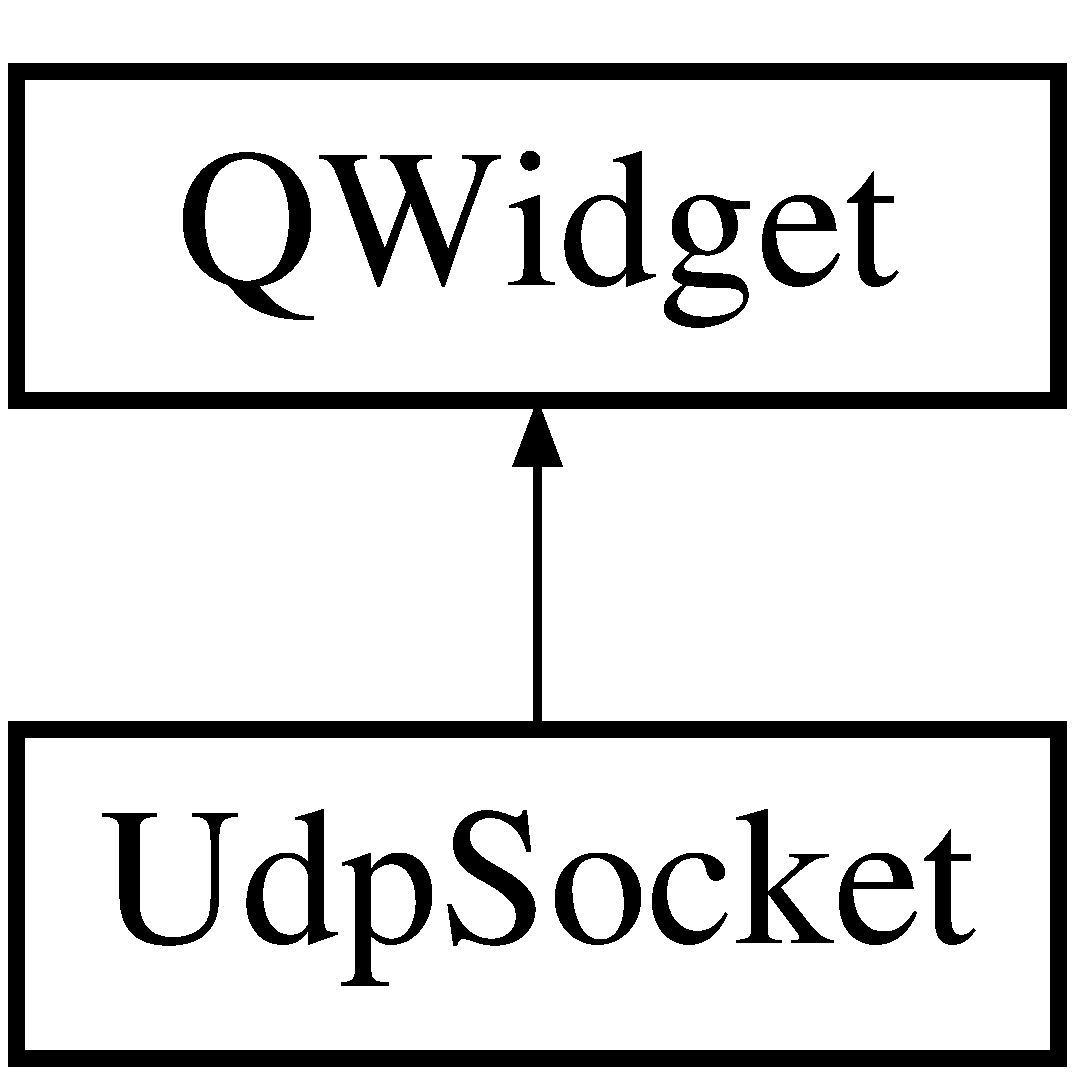
\includegraphics[height=2.000000cm]{classUdpSocket}
\end{center}
\end{figure}
\subsubsection*{Signals}
\begin{DoxyCompactItemize}
\item 
void \mbox{\hyperlink{classUdpSocket_a43ebbd10ee3b27bfe0b62b507bf8e2c4}{exit\+Req}} ()
\item 
void \mbox{\hyperlink{classUdpSocket_af24c4f2c6b77c9999e8638aead581477}{data\+Ready}} (Q\+Byte\+Array data)
\end{DoxyCompactItemize}
\subsubsection*{Public Member Functions}
\begin{DoxyCompactItemize}
\item 
\mbox{\hyperlink{classUdpSocket_a25a2f670352d9f600143c370beafd8f6}{Udp\+Socket}} (Q\+Widget $\ast$parent=0)
\item 
void \mbox{\hyperlink{classUdpSocket_aca3bb48ba03494ee09ed46a9e6d27ffb}{start\+Udp}} (bool \mbox{\hyperlink{classUdpSocket_aa5132ded0322787b898fa346a42f7dce}{is\+Master}}=true)
\item 
void \mbox{\hyperlink{classUdpSocket_a508506f2a8a7bbfa04a010ac491f9fa9}{stop\+Udp}} ()
\item 
void \mbox{\hyperlink{classUdpSocket_a1d66f093f85db5ae4df98a57adfeb322}{send\+Data}} (Q\+Byte\+Array b\+Arr)
\end{DoxyCompactItemize}
\subsubsection*{Private Slots}
\begin{DoxyCompactItemize}
\item 
void \mbox{\hyperlink{classUdpSocket_a4c16ef2e336d0504adb9118455fa7154}{connect\+To\+Socket}} ()
\item 
void \mbox{\hyperlink{classUdpSocket_a35cee44b0c57e6e5ec24c692d2ef9fb8}{disconnect\+From\+Socket}} ()
\item 
void \mbox{\hyperlink{classUdpSocket_a5c7396705869aab2fd14770582aff025}{start\+Transmit}} (Q\+Byte\+Array data)
\item 
void \mbox{\hyperlink{classUdpSocket_aa6b5948ab613404d74717eb7d9526dfb}{recive\+Data}} ()
\end{DoxyCompactItemize}
\subsubsection*{Private Attributes}
\begin{DoxyCompactItemize}
\item 
Q\+Udp\+Socket $\ast$ \mbox{\hyperlink{classUdpSocket_ac8d766e026e7685c741f631acc64e906}{udp}}
\item 
Q\+Host\+Address \mbox{\hyperlink{classUdpSocket_abb938c7331685fd351d93be1cb0d8524}{udp\+Adr}}
\item 
quint16 \mbox{\hyperlink{classUdpSocket_a13ad80532191677ae811e88181bed986}{udp\+Port}}
\item 
bool \mbox{\hyperlink{classUdpSocket_aeffff5f69078361d1f7c088827cf651d}{search}}
\item 
bool \mbox{\hyperlink{classUdpSocket_aa5132ded0322787b898fa346a42f7dce}{is\+Master}}
\item 
Q\+Host\+Address \mbox{\hyperlink{classUdpSocket_a784b0938e5af88875f8de414d58e536a}{my\+IP}}
\end{DoxyCompactItemize}


\subsubsection{Constructor \& Destructor Documentation}
\mbox{\Hypertarget{classUdpSocket_a25a2f670352d9f600143c370beafd8f6}\label{classUdpSocket_a25a2f670352d9f600143c370beafd8f6}} 
\index{Udp\+Socket@{Udp\+Socket}!Udp\+Socket@{Udp\+Socket}}
\index{Udp\+Socket@{Udp\+Socket}!Udp\+Socket@{Udp\+Socket}}
{\footnotesize\ttfamily Udp\+Socket\+::\texorpdfstring{Udp\+Socket}{UdpSocket} (\begin{DoxyParamCaption}\item[{Q\+Widget $\ast$}]{parent = {\ttfamily 0} }\end{DoxyParamCaption})\hspace{0.3cm}{\ttfamily [explicit]}}



\subsubsection{Member Function Documentation}
\mbox{\Hypertarget{classUdpSocket_a4c16ef2e336d0504adb9118455fa7154}\label{classUdpSocket_a4c16ef2e336d0504adb9118455fa7154}} 
\index{Udp\+Socket@{Udp\+Socket}!connect\+To\+Socket@{connect\+To\+Socket}}
\index{connect\+To\+Socket@{connect\+To\+Socket}!Udp\+Socket@{Udp\+Socket}}
{\footnotesize\ttfamily void Udp\+Socket\+::\texorpdfstring{connect\+To\+Socket}{connectToSocket} (\begin{DoxyParamCaption}{ }\end{DoxyParamCaption})\hspace{0.3cm}{\ttfamily [private]}, {\ttfamily [slot]}}

\mbox{\Hypertarget{classUdpSocket_af24c4f2c6b77c9999e8638aead581477}\label{classUdpSocket_af24c4f2c6b77c9999e8638aead581477}} 
\index{Udp\+Socket@{Udp\+Socket}!data\+Ready@{data\+Ready}}
\index{data\+Ready@{data\+Ready}!Udp\+Socket@{Udp\+Socket}}
{\footnotesize\ttfamily void Udp\+Socket\+::\texorpdfstring{data\+Ready}{dataReady} (\begin{DoxyParamCaption}\item[{Q\+Byte\+Array}]{data }\end{DoxyParamCaption})\hspace{0.3cm}{\ttfamily [signal]}}

\mbox{\Hypertarget{classUdpSocket_a35cee44b0c57e6e5ec24c692d2ef9fb8}\label{classUdpSocket_a35cee44b0c57e6e5ec24c692d2ef9fb8}} 
\index{Udp\+Socket@{Udp\+Socket}!disconnect\+From\+Socket@{disconnect\+From\+Socket}}
\index{disconnect\+From\+Socket@{disconnect\+From\+Socket}!Udp\+Socket@{Udp\+Socket}}
{\footnotesize\ttfamily void Udp\+Socket\+::\texorpdfstring{disconnect\+From\+Socket}{disconnectFromSocket} (\begin{DoxyParamCaption}{ }\end{DoxyParamCaption})\hspace{0.3cm}{\ttfamily [private]}, {\ttfamily [slot]}}

\mbox{\Hypertarget{classUdpSocket_a43ebbd10ee3b27bfe0b62b507bf8e2c4}\label{classUdpSocket_a43ebbd10ee3b27bfe0b62b507bf8e2c4}} 
\index{Udp\+Socket@{Udp\+Socket}!exit\+Req@{exit\+Req}}
\index{exit\+Req@{exit\+Req}!Udp\+Socket@{Udp\+Socket}}
{\footnotesize\ttfamily void Udp\+Socket\+::\texorpdfstring{exit\+Req}{exitReq} (\begin{DoxyParamCaption}{ }\end{DoxyParamCaption})\hspace{0.3cm}{\ttfamily [signal]}}

\mbox{\Hypertarget{classUdpSocket_aa6b5948ab613404d74717eb7d9526dfb}\label{classUdpSocket_aa6b5948ab613404d74717eb7d9526dfb}} 
\index{Udp\+Socket@{Udp\+Socket}!recive\+Data@{recive\+Data}}
\index{recive\+Data@{recive\+Data}!Udp\+Socket@{Udp\+Socket}}
{\footnotesize\ttfamily void Udp\+Socket\+::\texorpdfstring{recive\+Data}{reciveData} (\begin{DoxyParamCaption}{ }\end{DoxyParamCaption})\hspace{0.3cm}{\ttfamily [private]}, {\ttfamily [slot]}}

\mbox{\Hypertarget{classUdpSocket_a1d66f093f85db5ae4df98a57adfeb322}\label{classUdpSocket_a1d66f093f85db5ae4df98a57adfeb322}} 
\index{Udp\+Socket@{Udp\+Socket}!send\+Data@{send\+Data}}
\index{send\+Data@{send\+Data}!Udp\+Socket@{Udp\+Socket}}
{\footnotesize\ttfamily void Udp\+Socket\+::\texorpdfstring{send\+Data}{sendData} (\begin{DoxyParamCaption}\item[{Q\+Byte\+Array}]{b\+Arr }\end{DoxyParamCaption})}

\mbox{\Hypertarget{classUdpSocket_a5c7396705869aab2fd14770582aff025}\label{classUdpSocket_a5c7396705869aab2fd14770582aff025}} 
\index{Udp\+Socket@{Udp\+Socket}!start\+Transmit@{start\+Transmit}}
\index{start\+Transmit@{start\+Transmit}!Udp\+Socket@{Udp\+Socket}}
{\footnotesize\ttfamily void Udp\+Socket\+::\texorpdfstring{start\+Transmit}{startTransmit} (\begin{DoxyParamCaption}\item[{Q\+Byte\+Array}]{data }\end{DoxyParamCaption})\hspace{0.3cm}{\ttfamily [private]}, {\ttfamily [slot]}}

\mbox{\Hypertarget{classUdpSocket_aca3bb48ba03494ee09ed46a9e6d27ffb}\label{classUdpSocket_aca3bb48ba03494ee09ed46a9e6d27ffb}} 
\index{Udp\+Socket@{Udp\+Socket}!start\+Udp@{start\+Udp}}
\index{start\+Udp@{start\+Udp}!Udp\+Socket@{Udp\+Socket}}
{\footnotesize\ttfamily void Udp\+Socket\+::\texorpdfstring{start\+Udp}{startUdp} (\begin{DoxyParamCaption}\item[{bool}]{is\+Master = {\ttfamily true} }\end{DoxyParamCaption})}

\mbox{\Hypertarget{classUdpSocket_a508506f2a8a7bbfa04a010ac491f9fa9}\label{classUdpSocket_a508506f2a8a7bbfa04a010ac491f9fa9}} 
\index{Udp\+Socket@{Udp\+Socket}!stop\+Udp@{stop\+Udp}}
\index{stop\+Udp@{stop\+Udp}!Udp\+Socket@{Udp\+Socket}}
{\footnotesize\ttfamily void Udp\+Socket\+::\texorpdfstring{stop\+Udp}{stopUdp} (\begin{DoxyParamCaption}{ }\end{DoxyParamCaption})}



\subsubsection{Member Data Documentation}
\mbox{\Hypertarget{classUdpSocket_aa5132ded0322787b898fa346a42f7dce}\label{classUdpSocket_aa5132ded0322787b898fa346a42f7dce}} 
\index{Udp\+Socket@{Udp\+Socket}!is\+Master@{is\+Master}}
\index{is\+Master@{is\+Master}!Udp\+Socket@{Udp\+Socket}}
{\footnotesize\ttfamily bool Udp\+Socket\+::\texorpdfstring{is\+Master}{isMaster}\hspace{0.3cm}{\ttfamily [private]}}

\mbox{\Hypertarget{classUdpSocket_a784b0938e5af88875f8de414d58e536a}\label{classUdpSocket_a784b0938e5af88875f8de414d58e536a}} 
\index{Udp\+Socket@{Udp\+Socket}!my\+IP@{my\+IP}}
\index{my\+IP@{my\+IP}!Udp\+Socket@{Udp\+Socket}}
{\footnotesize\ttfamily Q\+Host\+Address Udp\+Socket\+::\texorpdfstring{my\+IP}{myIP}\hspace{0.3cm}{\ttfamily [private]}}

\mbox{\Hypertarget{classUdpSocket_aeffff5f69078361d1f7c088827cf651d}\label{classUdpSocket_aeffff5f69078361d1f7c088827cf651d}} 
\index{Udp\+Socket@{Udp\+Socket}!search@{search}}
\index{search@{search}!Udp\+Socket@{Udp\+Socket}}
{\footnotesize\ttfamily bool Udp\+Socket\+::\texorpdfstring{search}{search}\hspace{0.3cm}{\ttfamily [private]}}

\mbox{\Hypertarget{classUdpSocket_ac8d766e026e7685c741f631acc64e906}\label{classUdpSocket_ac8d766e026e7685c741f631acc64e906}} 
\index{Udp\+Socket@{Udp\+Socket}!udp@{udp}}
\index{udp@{udp}!Udp\+Socket@{Udp\+Socket}}
{\footnotesize\ttfamily Q\+Udp\+Socket$\ast$ Udp\+Socket\+::\texorpdfstring{udp}{udp}\hspace{0.3cm}{\ttfamily [private]}}

\mbox{\Hypertarget{classUdpSocket_abb938c7331685fd351d93be1cb0d8524}\label{classUdpSocket_abb938c7331685fd351d93be1cb0d8524}} 
\index{Udp\+Socket@{Udp\+Socket}!udp\+Adr@{udp\+Adr}}
\index{udp\+Adr@{udp\+Adr}!Udp\+Socket@{Udp\+Socket}}
{\footnotesize\ttfamily Q\+Host\+Address Udp\+Socket\+::\texorpdfstring{udp\+Adr}{udpAdr}\hspace{0.3cm}{\ttfamily [private]}}

\mbox{\Hypertarget{classUdpSocket_a13ad80532191677ae811e88181bed986}\label{classUdpSocket_a13ad80532191677ae811e88181bed986}} 
\index{Udp\+Socket@{Udp\+Socket}!udp\+Port@{udp\+Port}}
\index{udp\+Port@{udp\+Port}!Udp\+Socket@{Udp\+Socket}}
{\footnotesize\ttfamily quint16 Udp\+Socket\+::\texorpdfstring{udp\+Port}{udpPort}\hspace{0.3cm}{\ttfamily [private]}}



The documentation for this class was generated from the following files\+:\begin{DoxyCompactItemize}
\item 
\mbox{\hyperlink{udpsocket_8h}{udpsocket.\+h}}\item 
\mbox{\hyperlink{udpsocket_8cpp}{udpsocket.\+cpp}}\end{DoxyCompactItemize}
\newpage
\hypertarget{classUserSettingDialog}{}\subsection{User\+Setting\+Dialog Class Reference}
\label{classUserSettingDialog}\index{User\+Setting\+Dialog@{User\+Setting\+Dialog}}


{\ttfamily \#include $<$usersetting.\+h$>$}

Inheritance diagram for User\+Setting\+Dialog\+:\begin{figure}[H]
\begin{center}
\leavevmode
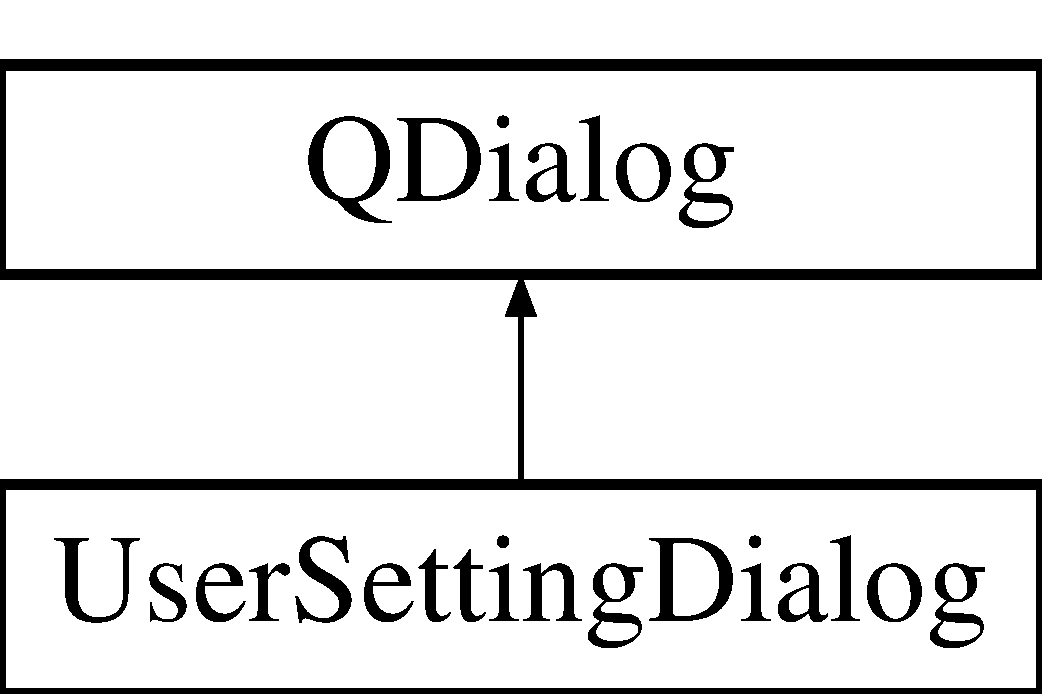
\includegraphics[height=2.000000cm]{classUserSettingDialog}
\end{center}
\end{figure}
\subsubsection*{Public Member Functions}
\begin{DoxyCompactItemize}
\item 
\mbox{\hyperlink{classUserSettingDialog_a8d3526dd76e3bf77fb8e02e1febeb8e4}{User\+Setting\+Dialog}} (Q\+Widget $\ast$parent=0)
\item 
\mbox{\hyperlink{classUserSettingDialog_a49def01d834dfdd9df00ce9fd6c6f4dc}{$\sim$\+User\+Setting\+Dialog}} ()
\item 
bool \mbox{\hyperlink{classUserSettingDialog_a10640f3e9a3935beba233c3bf7f1bb63}{is\+User}} (Q\+String user\+Name, Q\+String user\+Passw)
\item 
Q\+String\+List \mbox{\hyperlink{classUserSettingDialog_a96352f86848e37e60ef1b47c410ea676}{get\+User\+Names}} ()
\item 
bool \mbox{\hyperlink{classUserSettingDialog_a168420a490436fdb3a3b101b7e4e9fe3}{get\+Login\+Window\+Enable}} ()
\end{DoxyCompactItemize}
\subsubsection*{Protected Member Functions}
\begin{DoxyCompactItemize}
\item 
void \mbox{\hyperlink{classUserSettingDialog_ad1fd64225d23d8d49e9599aeffb9a235}{show\+Event}} (Q\+Show\+Event $\ast$ev)
\item 
void \mbox{\hyperlink{classUserSettingDialog_ad3b91400bb71ef025235bd9bee2551ac}{change\+Event}} (Q\+Event $\ast$event)
\end{DoxyCompactItemize}
\subsubsection*{Private Slots}
\begin{DoxyCompactItemize}
\item 
void \mbox{\hyperlink{classUserSettingDialog_adadac0b6a157e4fc15b5490f4e15b672}{table\+Cell\+Activated}} (int row, int col)
\item 
void \mbox{\hyperlink{classUserSettingDialog_a699172ed3d826f47823a5c7b2ee01cba}{add\+User}} ()
\item 
void \mbox{\hyperlink{classUserSettingDialog_a0c45242e9e0dc1ad4cf1960cca3575a4}{remove\+Users}} ()
\item 
void \mbox{\hyperlink{classUserSettingDialog_a5f4c353f8768d0225ac84f85607c4b54}{remove\+All\+Users}} ()
\item 
void \mbox{\hyperlink{classUserSettingDialog_a2efff8a9633f90bd27c990180b87b104}{accept\+Slot}} ()
\item 
void \mbox{\hyperlink{classUserSettingDialog_a46828cbc27d2dd2c587388090207dd8e}{reject\+Slot}} ()
\item 
void \mbox{\hyperlink{classUserSettingDialog_a9d077edc4d7cc247f8e57d1d6e8d7f89}{login\+Dialog\+Enable}} ()
\end{DoxyCompactItemize}
\subsubsection*{Private Attributes}
\begin{DoxyCompactItemize}
\item 
Ui\+::\+User\+Setting\+Dialog $\ast$ \mbox{\hyperlink{classUserSettingDialog_a915e2e661a7fe6fd265ec878f749cc82}{ui}}
\item 
int \mbox{\hyperlink{classUserSettingDialog_a965aa0e041af26cff9011bd8a04ad84c}{table\+Row\+Selected}}
\item 
int \mbox{\hyperlink{classUserSettingDialog_af4035cc2f93695c059c82ecd28ea70c8}{table\+Colnum\+Selected}}
\item 
Q\+Settings $\ast$ \mbox{\hyperlink{classUserSettingDialog_a2ea2a798911a3e2840542d7190613027}{users\+Data}}
\end{DoxyCompactItemize}


\subsubsection{Constructor \& Destructor Documentation}
\mbox{\Hypertarget{classUserSettingDialog_a8d3526dd76e3bf77fb8e02e1febeb8e4}\label{classUserSettingDialog_a8d3526dd76e3bf77fb8e02e1febeb8e4}} 
\index{User\+Setting\+Dialog@{User\+Setting\+Dialog}!User\+Setting\+Dialog@{User\+Setting\+Dialog}}
\index{User\+Setting\+Dialog@{User\+Setting\+Dialog}!User\+Setting\+Dialog@{User\+Setting\+Dialog}}
{\footnotesize\ttfamily User\+Setting\+Dialog\+::\texorpdfstring{User\+Setting\+Dialog}{UserSettingDialog} (\begin{DoxyParamCaption}\item[{Q\+Widget $\ast$}]{parent = {\ttfamily 0} }\end{DoxyParamCaption})\hspace{0.3cm}{\ttfamily [explicit]}} - standard dialog constructor. At function fields of dialog fills with appropriate data.

\mbox{\Hypertarget{classUserSettingDialog_a49def01d834dfdd9df00ce9fd6c6f4dc}\label{classUserSettingDialog_a49def01d834dfdd9df00ce9fd6c6f4dc}} 
\index{User\+Setting\+Dialog@{User\+Setting\+Dialog}!````~User\+Setting\+Dialog@{$\sim$\+User\+Setting\+Dialog}}
\index{````~User\+Setting\+Dialog@{$\sim$\+User\+Setting\+Dialog}!User\+Setting\+Dialog@{User\+Setting\+Dialog}}
{\footnotesize\ttfamily User\+Setting\+Dialog\+::\texorpdfstring{$\sim$\+User\+Setting\+Dialog}{~UserSettingDialog} (\begin{DoxyParamCaption}{ }\end{DoxyParamCaption})} - standatrd QDialog destructor.



\subsubsection{Member Function Documentation}
\mbox{\Hypertarget{classUserSettingDialog_a2efff8a9633f90bd27c990180b87b104}\label{classUserSettingDialog_a2efff8a9633f90bd27c990180b87b104}} 
\index{User\+Setting\+Dialog@{User\+Setting\+Dialog}!accept\+Slot@{accept\+Slot}}
\index{accept\+Slot@{accept\+Slot}!User\+Setting\+Dialog@{User\+Setting\+Dialog}}
{\footnotesize\ttfamily void User\+Setting\+Dialog\+::\texorpdfstring{accept\+Slot}{acceptSlot} (\begin{DoxyParamCaption}{ }\end{DoxyParamCaption})\hspace{0.3cm}{\ttfamily [private]}, {\ttfamily [slot]}} - function called by \textit{pButtonOK} uad used to collect and save data from fields of dialog.

\mbox{\Hypertarget{classUserSettingDialog_a699172ed3d826f47823a5c7b2ee01cba}\label{classUserSettingDialog_a699172ed3d826f47823a5c7b2ee01cba}} 
\index{User\+Setting\+Dialog@{User\+Setting\+Dialog}!add\+User@{add\+User}}
\index{add\+User@{add\+User}!User\+Setting\+Dialog@{User\+Setting\+Dialog}}
{\footnotesize\ttfamily void User\+Setting\+Dialog\+::\texorpdfstring{add\+User}{addUser} (\begin{DoxyParamCaption}{ }\end{DoxyParamCaption})\hspace{0.3cm}{\ttfamily [private]}, {\ttfamily [slot]}} - function which used to add field to \textit{tableWidget} to add new user.

\mbox{\Hypertarget{classUserSettingDialog_ad3b91400bb71ef025235bd9bee2551ac}\label{classUserSettingDialog_ad3b91400bb71ef025235bd9bee2551ac}} 
\index{User\+Setting\+Dialog@{User\+Setting\+Dialog}!change\+Event@{change\+Event}}
\index{change\+Event@{change\+Event}!User\+Setting\+Dialog@{User\+Setting\+Dialog}}
{\footnotesize\ttfamily void User\+Setting\+Dialog\+::\texorpdfstring{change\+Event}{changeEvent} (\begin{DoxyParamCaption}\item[{Q\+Event $\ast$}]{event }\end{DoxyParamCaption})\hspace{0.3cm}{\ttfamily [protected]}} - Reimplementation of default event for QWidget to enable user interface translation. Function called automatically.

\mbox{\Hypertarget{classUserSettingDialog_a168420a490436fdb3a3b101b7e4e9fe3}\label{classUserSettingDialog_a168420a490436fdb3a3b101b7e4e9fe3}} 
\index{User\+Setting\+Dialog@{User\+Setting\+Dialog}!get\+Login\+Window\+Enable@{get\+Login\+Window\+Enable}}
\index{get\+Login\+Window\+Enable@{get\+Login\+Window\+Enable}!User\+Setting\+Dialog@{User\+Setting\+Dialog}}
\paragraph{}
{\footnotesize\ttfamily bool User\+Setting\+Dialog\+::\texorpdfstring{get\+Login\+Window\+Enable}{getLoginWindowEnable} (\begin{DoxyParamCaption}{ }\end{DoxyParamCaption})} - function to get state of \textit{checkBoxLoginDialogEn}. Used to decide on the need to call user login dialog.

\mbox{\Hypertarget{classUserSettingDialog_a96352f86848e37e60ef1b47c410ea676}\label{classUserSettingDialog_a96352f86848e37e60ef1b47c410ea676}} 
\index{User\+Setting\+Dialog@{User\+Setting\+Dialog}!get\+User\+Names@{get\+User\+Names}}
\index{get\+User\+Names@{get\+User\+Names}!User\+Setting\+Dialog@{User\+Setting\+Dialog}}
{\footnotesize\ttfamily Q\+String\+List User\+Setting\+Dialog\+::\texorpdfstring{get\+User\+Names}{getUserNames} (\begin{DoxyParamCaption}{ }\end{DoxyParamCaption})} - function used to take \textit{QStringList} with names of users.

\mbox{\Hypertarget{classUserSettingDialog_a10640f3e9a3935beba233c3bf7f1bb63}\label{classUserSettingDialog_a10640f3e9a3935beba233c3bf7f1bb63}} 
\index{User\+Setting\+Dialog@{User\+Setting\+Dialog}!is\+User@{is\+User}}
\index{is\+User@{is\+User}!User\+Setting\+Dialog@{User\+Setting\+Dialog}}
{\footnotesize\ttfamily bool User\+Setting\+Dialog\+::\texorpdfstring{is\+User}{isUser} (\begin{DoxyParamCaption}\item[{Q\+String}]{user\+Name,  }\item[{Q\+String}]{user\+Passw }\end{DoxyParamCaption})} - function to check user name and password.

\mbox{\Hypertarget{classUserSettingDialog_a9d077edc4d7cc247f8e57d1d6e8d7f89}\label{classUserSettingDialog_a9d077edc4d7cc247f8e57d1d6e8d7f89}} 
\index{User\+Setting\+Dialog@{User\+Setting\+Dialog}!login\+Dialog\+Enable@{login\+Dialog\+Enable}}
\index{login\+Dialog\+Enable@{login\+Dialog\+Enable}!User\+Setting\+Dialog@{User\+Setting\+Dialog}}
{\footnotesize\ttfamily void User\+Setting\+Dialog\+::\texorpdfstring{login\+Dialog\+Enable}{loginDialogEnable} (\begin{DoxyParamCaption}{ }\end{DoxyParamCaption})\hspace{0.3cm}{\ttfamily [private]}, {\ttfamily [slot]}} - function to get field \textit{LOGIN\_DIALOG\_EN} from \hyperlink{classUserSettingDialog_a2ea2a798911a3e2840542d7190613027}{users\+Data} settings.

\mbox{\Hypertarget{classUserSettingDialog_a46828cbc27d2dd2c587388090207dd8e}\label{classUserSettingDialog_a46828cbc27d2dd2c587388090207dd8e}} 
\index{User\+Setting\+Dialog@{User\+Setting\+Dialog}!reject\+Slot@{reject\+Slot}}
\index{reject\+Slot@{reject\+Slot}!User\+Setting\+Dialog@{User\+Setting\+Dialog}}
{\footnotesize\ttfamily void User\+Setting\+Dialog\+::\texorpdfstring{reject\+Slot}{rejectSlot} (\begin{DoxyParamCaption}{ }\end{DoxyParamCaption})\hspace{0.3cm}{\ttfamily [private]}, {\ttfamily [slot]}} - function which used to close dialog without data saving.

\mbox{\Hypertarget{classUserSettingDialog_a5f4c353f8768d0225ac84f85607c4b54}\label{classUserSettingDialog_a5f4c353f8768d0225ac84f85607c4b54}} 
\index{User\+Setting\+Dialog@{User\+Setting\+Dialog}!remove\+All\+Users@{remove\+All\+Users}}
\index{remove\+All\+Users@{remove\+All\+Users}!User\+Setting\+Dialog@{User\+Setting\+Dialog}}
{\footnotesize\ttfamily void User\+Setting\+Dialog\+::\texorpdfstring{remove\+All\+Users}{removeAllUsers} (\begin{DoxyParamCaption}{ }\end{DoxyParamCaption})\hspace{0.3cm}{\ttfamily [private]}, {\ttfamily [slot]}} - function to clean \textit{tableWidget}.

\mbox{\Hypertarget{classUserSettingDialog_a0c45242e9e0dc1ad4cf1960cca3575a4}\label{classUserSettingDialog_a0c45242e9e0dc1ad4cf1960cca3575a4}} 
\index{User\+Setting\+Dialog@{User\+Setting\+Dialog}!remove\+Users@{remove\+Users}}
\index{remove\+Users@{remove\+Users}!User\+Setting\+Dialog@{User\+Setting\+Dialog}}
{\footnotesize\ttfamily void User\+Setting\+Dialog\+::\texorpdfstring{remove\+Users}{removeUsers} (\begin{DoxyParamCaption}{ }\end{DoxyParamCaption})\hspace{0.3cm}{\ttfamily [private]}, {\ttfamily [slot]}} - function to remove selected row from \textit{tableWidget}.

\mbox{\Hypertarget{classUserSettingDialog_ad1fd64225d23d8d49e9599aeffb9a235}\label{classUserSettingDialog_ad1fd64225d23d8d49e9599aeffb9a235}} 
\index{User\+Setting\+Dialog@{User\+Setting\+Dialog}!show\+Event@{show\+Event}}
\index{show\+Event@{show\+Event}!User\+Setting\+Dialog@{User\+Setting\+Dialog}}
{\footnotesize\ttfamily void User\+Setting\+Dialog\+::\texorpdfstring{show\+Event}{showEvent} (\begin{DoxyParamCaption}\item[{Q\+Show\+Event $\ast$}]{ev }\end{DoxyParamCaption})\hspace{0.3cm}{\ttfamily [protected]}} - reimplementation of standard function. Used to setup parameters of \textit{tableWidget}.

\mbox{\Hypertarget{classUserSettingDialog_adadac0b6a157e4fc15b5490f4e15b672}\label{classUserSettingDialog_adadac0b6a157e4fc15b5490f4e15b672}} 
\index{User\+Setting\+Dialog@{User\+Setting\+Dialog}!table\+Cell\+Activated@{table\+Cell\+Activated}}
\index{table\+Cell\+Activated@{table\+Cell\+Activated}!User\+Setting\+Dialog@{User\+Setting\+Dialog}}
{\footnotesize\ttfamily void User\+Setting\+Dialog\+::\texorpdfstring{table\+Cell\+Activated}{tableCellActivated} (\begin{DoxyParamCaption}\item[{int}]{row,  }\item[{int}]{col }\end{DoxyParamCaption})\hspace{0.3cm}{\ttfamily [private]}, {\ttfamily [slot]}} - function called by \textit{cellClicked}(...) signal. Used ro set value of \hyperlink{classUserSettingDialog_a965aa0e041af26cff9011bd8a04ad84c}{table\+Row\+Selected} and \hyperlink{classUserSettingDialog_af4035cc2f93695c059c82ecd28ea70c8}{table\+Colnum\+Selected} to use that values at other functions.


\subsubsection{Member Data Documentation}
\mbox{\Hypertarget{classUserSettingDialog_af4035cc2f93695c059c82ecd28ea70c8}\label{classUserSettingDialog_af4035cc2f93695c059c82ecd28ea70c8}} 
\index{User\+Setting\+Dialog@{User\+Setting\+Dialog}!table\+Colnum\+Selected@{table\+Colnum\+Selected}}
\index{table\+Colnum\+Selected@{table\+Colnum\+Selected}!User\+Setting\+Dialog@{User\+Setting\+Dialog}}
{\footnotesize\ttfamily int User\+Setting\+Dialog\+::\texorpdfstring{table\+Colnum\+Selected}{tableColnumSelected}\hspace{0.3cm}{\ttfamily [private]}}

\mbox{\Hypertarget{classUserSettingDialog_a965aa0e041af26cff9011bd8a04ad84c}\label{classUserSettingDialog_a965aa0e041af26cff9011bd8a04ad84c}} 
\index{User\+Setting\+Dialog@{User\+Setting\+Dialog}!table\+Row\+Selected@{table\+Row\+Selected}}
\index{table\+Row\+Selected@{table\+Row\+Selected}!User\+Setting\+Dialog@{User\+Setting\+Dialog}}
{\footnotesize\ttfamily int User\+Setting\+Dialog\+::\texorpdfstring{table\+Row\+Selected}{tableRowSelected}\hspace{0.3cm}{\ttfamily [private]}}

\mbox{\Hypertarget{classUserSettingDialog_a2ea2a798911a3e2840542d7190613027}\label{classUserSettingDialog_a2ea2a798911a3e2840542d7190613027}} 
\index{User\+Setting\+Dialog@{User\+Setting\+Dialog}!users\+Data@{users\+Data}}
\index{users\+Data@{users\+Data}!User\+Setting\+Dialog@{User\+Setting\+Dialog}}
{\footnotesize\ttfamily Q\+Settings$\ast$ User\+Setting\+Dialog\+::\texorpdfstring{users\+Data}{usersData}\hspace{0.3cm}{\ttfamily [private]}}



The documentation for this class was generated from the following files\+:\begin{DoxyCompactItemize}
\item 
\mbox{\hyperlink{usersetting_8h}{usersetting.\+h}}\item 
\mbox{\hyperlink{usersetting_8cpp}{usersetting.\+cpp}}\end{DoxyCompactItemize}
\newpage
\hypertarget{classWarmingWidget}{}\subsection{Warming\+Widget Class Reference}
\label{classWarmingWidget}\index{Warming\+Widget@{Warming\+Widget}}


{\ttfamily \#include $<$warmingwidget.\+h$>$}

Inheritance diagram for Warming\+Widget\+:\begin{figure}[H]
\begin{center}
\leavevmode
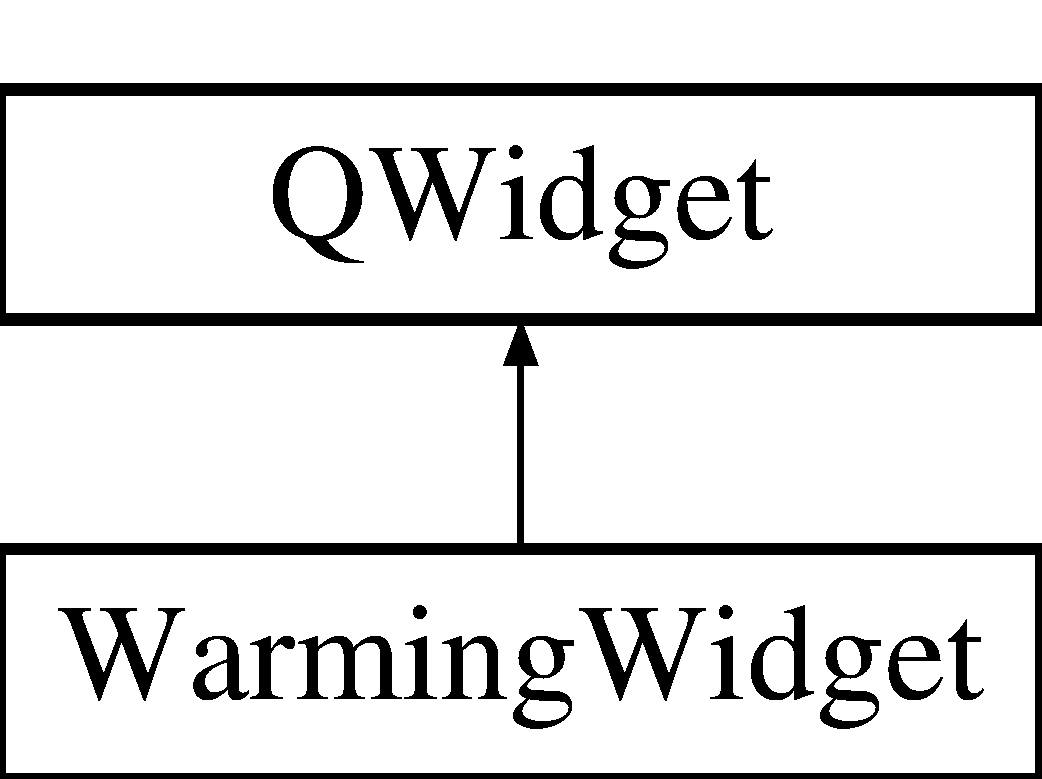
\includegraphics[height=2.000000cm]{classWarmingWidget}
\end{center}
\end{figure}
\subsubsection*{Signals}
\begin{DoxyCompactItemize}
\item 
void \hyperlink{classWarmingWidget_ab18f4c153590131b6f391b084a4351f4}{send\+Command} (Q\+Byte\+Array)
\end{DoxyCompactItemize}
\subsubsection*{Public Member Functions}
\begin{DoxyCompactItemize}
\item 
\hyperlink{classWarmingWidget_a99e5c7ec6836696b8b0d35415a0604e7}{Warming\+Widget} (Q\+Widget $\ast$parent=0)
\item 
\hyperlink{classWarmingWidget_a17ad9285138404c3dae609b9c8c64912}{$\sim$\+Warming\+Widget} ()
\item 
void \hyperlink{classWarmingWidget_a217bbee950a217a90e0a426d35f02f1d}{set\+Icon\+Folder} (Q\+String path)
\item 
void \hyperlink{classWarmingWidget_a15ba48978ff7a7f38ea2a09009af3162}{set\+Registers} (\hyperlink{classRegister}{Register} $\ast$reg)
\item 
void \hyperlink{classWarmingWidget_a4aa925700a3d51f16d1c61dcd447d503}{reset\+Widget} ()
\end{DoxyCompactItemize}
\subsubsection*{Protected Member Functions}
\begin{DoxyCompactItemize}
\item 
void \hyperlink{classWarmingWidget_aca4d5901fb6fa056dbcd01a0f90a2164}{show\+Event} (Q\+Show\+Event $\ast$ev)
\end{DoxyCompactItemize}
\subsubsection*{Private Slots}
\begin{DoxyCompactItemize}
\item 
void \hyperlink{classWarmingWidget_af6d7762dac4bb124e1ba6ba9ea86bbeb}{on\+\_\+tool\+Button\+\_\+clicked} ()
\item 
void \hyperlink{classWarmingWidget_a26b06ccfb9f84215772231e40d2bbb4b}{on\+\_\+d\+Spin\+Box\+Time\+\_\+value\+Changed} (double arg1)
\item 
void \hyperlink{classWarmingWidget_a319141e919d6115a68dd1324464a3d8f}{on\+\_\+d\+Spin\+Box\+Cycles\+\_\+value\+Changed} (double arg1)
\item 
void \hyperlink{classWarmingWidget_a37d44b7276671774f60932d87a2dcdb5}{on\+\_\+d\+Spin\+Box\+Temperature\+\_\+value\+Changed} (double arg1)
\end{DoxyCompactItemize}
\subsubsection*{Private Attributes}
\begin{DoxyCompactItemize}
\item 
Ui\+::\+Warming\+Widget $\ast$ \hyperlink{classWarmingWidget_ae2dad8434667ce8a34454989548084b2}{ui}
\item 
Q\+String \hyperlink{classWarmingWidget_a31c1abfa505e08fb4c5f9f34e82c7d15}{path\+Icon}
\item 
\hyperlink{classRegister}{Register} $\ast$ \hyperlink{classWarmingWidget_a83bc5e6ef3f7679874a3074a750266a9}{registers}
\end{DoxyCompactItemize}


\subsubsection{Constructor \& Destructor Documentation}
\index{Warming\+Widget@{Warming\+Widget}!Warming\+Widget@{Warming\+Widget}}
\index{Warming\+Widget@{Warming\+Widget}!Warming\+Widget@{Warming\+Widget}}
\paragraph[{\texorpdfstring{Warming\+Widget(\+Q\+Widget $\ast$parent=0)}{WarmingWidget(QWidget *parent=0)}}]{\setlength{\rightskip}{0pt plus 5cm}Warming\+Widget\+::\+Warming\+Widget (
\begin{DoxyParamCaption}
\item[{Q\+Widget $\ast$}]{parent = {\ttfamily 0}}
\end{DoxyParamCaption}
)\hspace{0.3cm}{\ttfamily [explicit]}}\hypertarget{classWarmingWidget_a99e5c7ec6836696b8b0d35415a0604e7}{}\label{classWarmingWidget_a99e5c7ec6836696b8b0d35415a0604e7}
\index{Warming\+Widget@{Warming\+Widget}!````~Warming\+Widget@{$\sim$\+Warming\+Widget}}
\index{````~Warming\+Widget@{$\sim$\+Warming\+Widget}!Warming\+Widget@{Warming\+Widget}}
\paragraph[{\texorpdfstring{$\sim$\+Warming\+Widget()}{~WarmingWidget()}}]{\setlength{\rightskip}{0pt plus 5cm}Warming\+Widget\+::$\sim$\+Warming\+Widget (
\begin{DoxyParamCaption}
{}
\end{DoxyParamCaption}
)}\hypertarget{classWarmingWidget_a17ad9285138404c3dae609b9c8c64912}{}\label{classWarmingWidget_a17ad9285138404c3dae609b9c8c64912}


\subsubsection{Member Function Documentation}
\index{Warming\+Widget@{Warming\+Widget}!on\+\_\+d\+Spin\+Box\+Cycles\+\_\+value\+Changed@{on\+\_\+d\+Spin\+Box\+Cycles\+\_\+value\+Changed}}
\index{on\+\_\+d\+Spin\+Box\+Cycles\+\_\+value\+Changed@{on\+\_\+d\+Spin\+Box\+Cycles\+\_\+value\+Changed}!Warming\+Widget@{Warming\+Widget}}
\paragraph[{\texorpdfstring{on\+\_\+d\+Spin\+Box\+Cycles\+\_\+value\+Changed}{on_dSpinBoxCycles_valueChanged}}]{\setlength{\rightskip}{0pt plus 5cm}void Warming\+Widget\+::on\+\_\+d\+Spin\+Box\+Cycles\+\_\+value\+Changed (
\begin{DoxyParamCaption}
\item[{double}]{arg1}
\end{DoxyParamCaption}
)\hspace{0.3cm}{\ttfamily [private]}, {\ttfamily [slot]}}\hypertarget{classWarmingWidget_a319141e919d6115a68dd1324464a3d8f}{}\label{classWarmingWidget_a319141e919d6115a68dd1324464a3d8f}
10 \index{Warming\+Widget@{Warming\+Widget}!on\+\_\+d\+Spin\+Box\+Temperature\+\_\+value\+Changed@{on\+\_\+d\+Spin\+Box\+Temperature\+\_\+value\+Changed}}
\index{on\+\_\+d\+Spin\+Box\+Temperature\+\_\+value\+Changed@{on\+\_\+d\+Spin\+Box\+Temperature\+\_\+value\+Changed}!Warming\+Widget@{Warming\+Widget}}
\paragraph[{\texorpdfstring{on\+\_\+d\+Spin\+Box\+Temperature\+\_\+value\+Changed}{on_dSpinBoxTemperature_valueChanged}}]{\setlength{\rightskip}{0pt plus 5cm}void Warming\+Widget\+::on\+\_\+d\+Spin\+Box\+Temperature\+\_\+value\+Changed (
\begin{DoxyParamCaption}
\item[{double}]{arg1}
\end{DoxyParamCaption}
)\hspace{0.3cm}{\ttfamily [private]}, {\ttfamily [slot]}}\hypertarget{classWarmingWidget_a37d44b7276671774f60932d87a2dcdb5}{}\label{classWarmingWidget_a37d44b7276671774f60932d87a2dcdb5}
10 \index{Warming\+Widget@{Warming\+Widget}!on\+\_\+d\+Spin\+Box\+Time\+\_\+value\+Changed@{on\+\_\+d\+Spin\+Box\+Time\+\_\+value\+Changed}}
\index{on\+\_\+d\+Spin\+Box\+Time\+\_\+value\+Changed@{on\+\_\+d\+Spin\+Box\+Time\+\_\+value\+Changed}!Warming\+Widget@{Warming\+Widget}}
\paragraph[{\texorpdfstring{on\+\_\+d\+Spin\+Box\+Time\+\_\+value\+Changed}{on_dSpinBoxTime_valueChanged}}]{\setlength{\rightskip}{0pt plus 5cm}void Warming\+Widget\+::on\+\_\+d\+Spin\+Box\+Time\+\_\+value\+Changed (
\begin{DoxyParamCaption}
\item[{double}]{arg1}
\end{DoxyParamCaption}
)\hspace{0.3cm}{\ttfamily [private]}, {\ttfamily [slot]}}\hypertarget{classWarmingWidget_a26b06ccfb9f84215772231e40d2bbb4b}{}\label{classWarmingWidget_a26b06ccfb9f84215772231e40d2bbb4b}
\index{Warming\+Widget@{Warming\+Widget}!on\+\_\+tool\+Button\+\_\+clicked@{on\+\_\+tool\+Button\+\_\+clicked}}
\index{on\+\_\+tool\+Button\+\_\+clicked@{on\+\_\+tool\+Button\+\_\+clicked}!Warming\+Widget@{Warming\+Widget}}
\paragraph[{\texorpdfstring{on\+\_\+tool\+Button\+\_\+clicked}{on_toolButton_clicked}}]{\setlength{\rightskip}{0pt plus 5cm}void Warming\+Widget\+::on\+\_\+tool\+Button\+\_\+clicked (
\begin{DoxyParamCaption}
{}
\end{DoxyParamCaption}
)\hspace{0.3cm}{\ttfamily [private]}, {\ttfamily [slot]}}\hypertarget{classWarmingWidget_af6d7762dac4bb124e1ba6ba9ea86bbeb}{}\label{classWarmingWidget_af6d7762dac4bb124e1ba6ba9ea86bbeb}
\index{Warming\+Widget@{Warming\+Widget}!reset\+Widget@{reset\+Widget}}
\index{reset\+Widget@{reset\+Widget}!Warming\+Widget@{Warming\+Widget}}
\paragraph[{\texorpdfstring{reset\+Widget()}{resetWidget()}}]{\setlength{\rightskip}{0pt plus 5cm}void Warming\+Widget\+::reset\+Widget (
\begin{DoxyParamCaption}
{}
\end{DoxyParamCaption}
)}\hypertarget{classWarmingWidget_a4aa925700a3d51f16d1c61dcd447d503}{}\label{classWarmingWidget_a4aa925700a3d51f16d1c61dcd447d503}
\index{Warming\+Widget@{Warming\+Widget}!send\+Command@{send\+Command}}
\index{send\+Command@{send\+Command}!Warming\+Widget@{Warming\+Widget}}
\paragraph[{\texorpdfstring{send\+Command}{sendCommand}}]{\setlength{\rightskip}{0pt plus 5cm}void Warming\+Widget\+::send\+Command (
\begin{DoxyParamCaption}
\item[{Q\+Byte\+Array}]{}
\end{DoxyParamCaption}
)\hspace{0.3cm}{\ttfamily [signal]}}\hypertarget{classWarmingWidget_ab18f4c153590131b6f391b084a4351f4}{}\label{classWarmingWidget_ab18f4c153590131b6f391b084a4351f4}
\index{Warming\+Widget@{Warming\+Widget}!set\+Icon\+Folder@{set\+Icon\+Folder}}
\index{set\+Icon\+Folder@{set\+Icon\+Folder}!Warming\+Widget@{Warming\+Widget}}
\paragraph[{\texorpdfstring{set\+Icon\+Folder(\+Q\+String path)}{setIconFolder(QString path)}}]{\setlength{\rightskip}{0pt plus 5cm}void Warming\+Widget\+::set\+Icon\+Folder (
\begin{DoxyParamCaption}
\item[{Q\+String}]{path}
\end{DoxyParamCaption}
)}\hypertarget{classWarmingWidget_a217bbee950a217a90e0a426d35f02f1d}{}\label{classWarmingWidget_a217bbee950a217a90e0a426d35f02f1d}
\index{Warming\+Widget@{Warming\+Widget}!set\+Registers@{set\+Registers}}
\index{set\+Registers@{set\+Registers}!Warming\+Widget@{Warming\+Widget}}
\paragraph[{\texorpdfstring{set\+Registers(\+Register $\ast$reg)}{setRegisters(Register *reg)}}]{\setlength{\rightskip}{0pt plus 5cm}void Warming\+Widget\+::set\+Registers (
\begin{DoxyParamCaption}
\item[{{\bf Register} $\ast$}]{reg}
\end{DoxyParamCaption}
)}\hypertarget{classWarmingWidget_a15ba48978ff7a7f38ea2a09009af3162}{}\label{classWarmingWidget_a15ba48978ff7a7f38ea2a09009af3162}
\index{Warming\+Widget@{Warming\+Widget}!show\+Event@{show\+Event}}
\index{show\+Event@{show\+Event}!Warming\+Widget@{Warming\+Widget}}
\paragraph[{\texorpdfstring{show\+Event(\+Q\+Show\+Event $\ast$ev)}{showEvent(QShowEvent *ev)}}]{\setlength{\rightskip}{0pt plus 5cm}void Warming\+Widget\+::show\+Event (
\begin{DoxyParamCaption}
\item[{Q\+Show\+Event $\ast$}]{ev}
\end{DoxyParamCaption}
)\hspace{0.3cm}{\ttfamily [protected]}}\hypertarget{classWarmingWidget_aca4d5901fb6fa056dbcd01a0f90a2164}{}\label{classWarmingWidget_aca4d5901fb6fa056dbcd01a0f90a2164}


\subsubsection{Member Data Documentation}
\index{Warming\+Widget@{Warming\+Widget}!path\+Icon@{path\+Icon}}
\index{path\+Icon@{path\+Icon}!Warming\+Widget@{Warming\+Widget}}
\paragraph[{\texorpdfstring{path\+Icon}{pathIcon}}]{\setlength{\rightskip}{0pt plus 5cm}Q\+String Warming\+Widget\+::path\+Icon\hspace{0.3cm}{\ttfamily [private]}}\hypertarget{classWarmingWidget_a31c1abfa505e08fb4c5f9f34e82c7d15}{}\label{classWarmingWidget_a31c1abfa505e08fb4c5f9f34e82c7d15}
\index{Warming\+Widget@{Warming\+Widget}!registers@{registers}}
\index{registers@{registers}!Warming\+Widget@{Warming\+Widget}}
\paragraph[{\texorpdfstring{registers}{registers}}]{\setlength{\rightskip}{0pt plus 5cm}{\bf Register}$\ast$ Warming\+Widget\+::registers\hspace{0.3cm}{\ttfamily [private]}}\hypertarget{classWarmingWidget_a83bc5e6ef3f7679874a3074a750266a9}{}\label{classWarmingWidget_a83bc5e6ef3f7679874a3074a750266a9}
\index{Warming\+Widget@{Warming\+Widget}!ui@{ui}}
\index{ui@{ui}!Warming\+Widget@{Warming\+Widget}}
\paragraph[{\texorpdfstring{ui}{ui}}]{\setlength{\rightskip}{0pt plus 5cm}Ui\+::\+Warming\+Widget$\ast$ Warming\+Widget\+::ui\hspace{0.3cm}{\ttfamily [private]}}\hypertarget{classWarmingWidget_ae2dad8434667ce8a34454989548084b2}{}\label{classWarmingWidget_ae2dad8434667ce8a34454989548084b2}


The documentation for this class was generated from the following files\+:\begin{DoxyCompactItemize}
\item 
\hyperlink{warmingwidget_8h}{warmingwidget.\+h}\item 
\hyperlink{warmingwidget_8cpp}{warmingwidget.\+cpp}\end{DoxyCompactItemize}

\section{File Documentation}
\hypertarget{countersdialog_8cpp}{}\subsection{countersdialog.\+cpp File Reference}
\label{countersdialog_8cpp}\index{countersdialog.\+cpp@{countersdialog.\+cpp}}
{\ttfamily \#include \char`\"{}countersdialog.\+h\char`\"{}}\\*
{\ttfamily \#include \char`\"{}ui\+\_\+countersdialog.\+h\char`\"{}}\\*

\hypertarget{countersdialog_8h}{}\subsection{countersdialog.\+h File Reference}
\label{countersdialog_8h}\index{countersdialog.\+h@{countersdialog.\+h}}
{\ttfamily \#include $<$Q\+Dialog$>$}\\*
{\ttfamily \#include $<$Q\+Show\+Event$>$}\\*
{\ttfamily \#include \char`\"{}numpaddialog.\+h\char`\"{}}\\*
\subsubsection*{Classes}
\begin{DoxyCompactItemize}
\item 
class \hyperlink{classCountersDialog}{Counters\+Dialog}
\end{DoxyCompactItemize}
\subsubsection*{Namespaces}
\begin{DoxyCompactItemize}
\item 
 \hyperlink{namespaceUi}{Ui}
\end{DoxyCompactItemize}

\hypertarget{crc16_8h}{}\subsection{crc16.\+h File Reference}
\label{crc16_8h}\index{crc16.\+h@{crc16.\+h}}
{\ttfamily \#include $<$stdio.\+h$>$}\newline
{\ttfamily \#include $<$stdint.\+h$>$}\newline
{\ttfamily \#include $<$Q\+Byte\+Array$>$}\newline
{\ttfamily \#include $<$Q\+Debug$>$}\newline
\subsubsection*{Classes}
\begin{DoxyCompactItemize}
\item 
class \mbox{\hyperlink{classCrcCalc}{Crc\+Calc}}
\end{DoxyCompactItemize}
\subsubsection*{Variables}
\begin{DoxyCompactItemize}
\item 
const \mbox{\hyperlink{settings_8h_a017dd44e68049ffdd31500a8cd01ba68}{uint16\+\_\+t}} \mbox{\hyperlink{crc16_8h_a6b39d3e505a20fcfc620f6902fb96b0d}{crctable}} \mbox{[}256\mbox{]}
\end{DoxyCompactItemize}


\subsubsection{Variable Documentation}
\mbox{\Hypertarget{crc16_8h_a6b39d3e505a20fcfc620f6902fb96b0d}\label{crc16_8h_a6b39d3e505a20fcfc620f6902fb96b0d}} 
\index{crc16.\+h@{crc16.\+h}!crctable@{crctable}}
\index{crctable@{crctable}!crc16.\+h@{crc16.\+h}}
\paragraph{\texorpdfstring{crctable}{crctable}}
{\footnotesize\ttfamily const \mbox{\hyperlink{settings_8h_a017dd44e68049ffdd31500a8cd01ba68}{uint16\+\_\+t}} crctable\mbox{[}256\mbox{]}}


\hypertarget{cyclesdialog_8cpp}{}\subsection{cyclesdialog.\+cpp File Reference}
\label{cyclesdialog_8cpp}\index{cyclesdialog.\+cpp@{cyclesdialog.\+cpp}}
{\ttfamily \#include \char`\"{}cyclesdialog.\+h\char`\"{}}\newline
{\ttfamily \#include \char`\"{}ui\+\_\+cyclesdialog.\+h\char`\"{}}\newline

\hypertarget{cyclesdialog_8h}{}\subsection{cyclesdialog.\+h File Reference}
\label{cyclesdialog_8h}\index{cyclesdialog.\+h@{cyclesdialog.\+h}}
{\ttfamily \#include $<$Q\+Dialog$>$}\newline
{\ttfamily \#include $<$Q\+Double\+Spin\+Box$>$}\newline
{\ttfamily \#include $<$Q\+Label$>$}\newline
{\ttfamily \#include $<$Q\+Line\+Edit$>$}\newline
{\ttfamily \#include $<$Q\+List$>$}\newline
{\ttfamily \#include $<$Q\+Show\+Event$>$}\newline
{\ttfamily \#include $<$Q\+Focus\+Event$>$}\newline
{\ttfamily \#include $<$Q\+Event$>$}\newline
{\ttfamily \#include $<$Q\+Settings$>$}\newline
{\ttfamily \#include $<$Q\+Byte\+Array$>$}\newline
{\ttfamily \#include \char`\"{}settings.\+h\char`\"{}}\newline
{\ttfamily \#include \char`\"{}numpaddialog.\+h\char`\"{}}\newline
{\ttfamily \#include \char`\"{}crc16.\+h\char`\"{}}\newline
{\ttfamily \#include $<$Q\+Debug$>$}\newline
\subsubsection*{Classes}
\begin{DoxyCompactItemize}
\item 
class \mbox{\hyperlink{classCyclesDialog}{Cycles\+Dialog}}
\end{DoxyCompactItemize}
\subsubsection*{Namespaces}
\begin{DoxyCompactItemize}
\item 
 \mbox{\hyperlink{namespaceUi}{Ui}}
\end{DoxyCompactItemize}

\hypertarget{exitdialog_8cpp}{}\subsection{exitdialog.\+cpp File Reference}
\label{exitdialog_8cpp}\index{exitdialog.\+cpp@{exitdialog.\+cpp}}
{\ttfamily \#include \char`\"{}exitdialog.\+h\char`\"{}}\newline
{\ttfamily \#include \char`\"{}ui\+\_\+exitdialog.\+h\char`\"{}}\newline

\hypertarget{exitdialog_8h}{}\subsection{exitdialog.\+h File Reference}
\label{exitdialog_8h}\index{exitdialog.\+h@{exitdialog.\+h}}
{\ttfamily \#include $<$Q\+Dialog$>$}\newline
{\ttfamily \#include $<$Q\+Show\+Event$>$}\newline
{\ttfamily \#include \char`\"{}settings.\+h\char`\"{}}\newline
\subsubsection*{Classes}
\begin{DoxyCompactItemize}
\item 
class \mbox{\hyperlink{classExitDialog}{Exit\+Dialog}}
\end{DoxyCompactItemize}
\subsubsection*{Namespaces}
\begin{DoxyCompactItemize}
\item 
 \mbox{\hyperlink{namespaceUi}{Ui}}
\end{DoxyCompactItemize}

\hypertarget{generalsettingdialog_8cpp}{}\subsection{generalsettingdialog.\+cpp File Reference}
\label{generalsettingdialog_8cpp}\index{generalsettingdialog.\+cpp@{generalsettingdialog.\+cpp}}
{\ttfamily \#include \char`\"{}generalsettingdialog.\+h\char`\"{}}\newline
{\ttfamily \#include \char`\"{}ui\+\_\+generalsettingdialog.\+h\char`\"{}}\newline
{\ttfamily \#include \char`\"{}crc16.\+h\char`\"{}}\newline

\hypertarget{generalsettingdialog_8h}{}\subsection{generalsettingdialog.\+h File Reference}
\label{generalsettingdialog_8h}\index{generalsettingdialog.\+h@{generalsettingdialog.\+h}}
{\ttfamily \#include $<$Q\+Dialog$>$}\newline
{\ttfamily \#include $<$Q\+String$>$}\newline
{\ttfamily \#include $<$Q\+Debug$>$}\newline
{\ttfamily \#include $<$Q\+Byte\+Array$>$}\newline
{\ttfamily \#include $<$Q\+Message\+Box$>$}\newline
{\ttfamily \#include $<$Q\+Input\+Dialog$>$}\newline
{\ttfamily \#include $<$Q\+Show\+Event$>$}\newline
{\ttfamily \#include \char`\"{}settings.\+h\char`\"{}}\newline
{\ttfamily \#include \char`\"{}numpaddialog.\+h\char`\"{}}\newline
{\ttfamily \#include \char`\"{}keyboarddialog.\+h\char`\"{}}\newline
{\ttfamily \#include \char`\"{}serialsettingsdialog.\+h\char`\"{}}\newline
\subsubsection*{Classes}
\begin{DoxyCompactItemize}
\item 
struct \mbox{\hyperlink{structEmailSettings}{Email\+Settings}}
\item 
class \mbox{\hyperlink{classGeneralSettingDialog}{General\+Setting\+Dialog}}
\end{DoxyCompactItemize}
\subsubsection*{Namespaces}
\begin{DoxyCompactItemize}
\item 
 \mbox{\hyperlink{namespaceUi}{Ui}}
\end{DoxyCompactItemize}
\subsubsection*{Functions}
\begin{DoxyCompactItemize}
\item 
Q\+Data\+Stream \& \mbox{\hyperlink{generalsettingdialog_8h_a1afeb5eeab9e861aff78a6fd00c243cb}{operator$<$$<$}} (Q\+Data\+Stream \&out, const \mbox{\hyperlink{structEmailSettings}{Email\+Settings}} \&st)
\item 
Q\+Data\+Stream \& \mbox{\hyperlink{generalsettingdialog_8h_a27de9a59b136eb044435af81c7f4fadb}{operator$>$$>$}} (Q\+Data\+Stream \&in, \mbox{\hyperlink{structEmailSettings}{Email\+Settings}} \&st)
\end{DoxyCompactItemize}


\subsubsection{Function Documentation}
\mbox{\Hypertarget{generalsettingdialog_8h_a1afeb5eeab9e861aff78a6fd00c243cb}\label{generalsettingdialog_8h_a1afeb5eeab9e861aff78a6fd00c243cb}} 
\index{generalsettingdialog.\+h@{generalsettingdialog.\+h}!operator$<$$<$@{operator$<$$<$}}
\index{operator$<$$<$@{operator$<$$<$}!generalsettingdialog.\+h@{generalsettingdialog.\+h}}
\paragraph{\texorpdfstring{operator$<$$<$()}{operator<<()}}
{\footnotesize\ttfamily Q\+Data\+Stream\& operator$<$$<$ (\begin{DoxyParamCaption}\item[{Q\+Data\+Stream \&}]{out,  }\item[{const \mbox{\hyperlink{structEmailSettings}{Email\+Settings}} \&}]{st }\end{DoxyParamCaption})\hspace{0.3cm}{\ttfamily [inline]}}

\mbox{\Hypertarget{generalsettingdialog_8h_a27de9a59b136eb044435af81c7f4fadb}\label{generalsettingdialog_8h_a27de9a59b136eb044435af81c7f4fadb}} 
\index{generalsettingdialog.\+h@{generalsettingdialog.\+h}!operator$>$$>$@{operator$>$$>$}}
\index{operator$>$$>$@{operator$>$$>$}!generalsettingdialog.\+h@{generalsettingdialog.\+h}}
\paragraph{\texorpdfstring{operator$>$$>$()}{operator>>()}}
{\footnotesize\ttfamily Q\+Data\+Stream\& operator$>$$>$ (\begin{DoxyParamCaption}\item[{Q\+Data\+Stream \&}]{in,  }\item[{\mbox{\hyperlink{structEmailSettings}{Email\+Settings}} \&}]{st }\end{DoxyParamCaption})\hspace{0.3cm}{\ttfamily [inline]}}


\hypertarget{headactivationdialog_8cpp}{}\subsection{headactivationdialog.\+cpp File Reference}
\label{headactivationdialog_8cpp}\index{headactivationdialog.\+cpp@{headactivationdialog.\+cpp}}
{\ttfamily \#include \char`\"{}headactivationdialog.\+h\char`\"{}}\newline
{\ttfamily \#include \char`\"{}ui\+\_\+headactivationdialog.\+h\char`\"{}}\newline

\hypertarget{headactivationdialog_8h}{}\subsection{headactivationdialog.\+h File Reference}
\label{headactivationdialog_8h}\index{headactivationdialog.\+h@{headactivationdialog.\+h}}
{\ttfamily \#include $<$Q\+Dialog$>$}\newline
{\ttfamily \#include $<$Q\+Check\+Box$>$}\newline
{\ttfamily \#include $<$Q\+List$>$}\newline
{\ttfamily \#include $<$Q\+Show\+Event$>$}\newline
{\ttfamily \#include $<$Q\+Debug$>$}\newline
{\ttfamily \#include \char`\"{}settings.\+h\char`\"{}}\newline
{\ttfamily \#include \char`\"{}crc16.\+h\char`\"{}}\newline
\subsubsection*{Classes}
\begin{DoxyCompactItemize}
\item 
class \mbox{\hyperlink{classCheckBoxIndexed}{Check\+Box\+Indexed}}
\item 
class \mbox{\hyperlink{classHeadActivationDialog}{Head\+Activation\+Dialog}}
\end{DoxyCompactItemize}
\subsubsection*{Namespaces}
\begin{DoxyCompactItemize}
\item 
 \mbox{\hyperlink{namespaceUi}{Ui}}
\end{DoxyCompactItemize}

\hypertarget{headform_8cpp}{}\subsection{headform.\+cpp File Reference}
\label{headform_8cpp}\index{headform.\+cpp@{headform.\+cpp}}
{\ttfamily \#include \char`\"{}headform.\+h\char`\"{}}\newline
{\ttfamily \#include \char`\"{}ui\+\_\+headform.\+h\char`\"{}}\newline
{\ttfamily \#include $<$Q\+Bitmap$>$}\newline
{\ttfamily \#include $<$Q\+Palette$>$}\newline

\hypertarget{headform_8h}{}\subsection{headform.\+h File Reference}
\label{headform_8h}\index{headform.\+h@{headform.\+h}}
{\ttfamily \#include $<$Q\+Widget$>$}\newline
{\ttfamily \#include $<$Q\+Pixmap$>$}\newline
{\ttfamily \#include $<$Q\+Push\+Button$>$}\newline
{\ttfamily \#include $<$Q\+Label$>$}\newline
{\ttfamily \#include $<$Q\+Mouse\+Event$>$}\newline
{\ttfamily \#include $<$Q\+Debug$>$}\newline
{\ttfamily \#include $<$Q\+Graphics\+Effect$>$}\newline
{\ttfamily \#include $<$Q\+Graphics\+Scene$>$}\newline
{\ttfamily \#include $<$Q\+Graphics\+Rect\+Item$>$}\newline
{\ttfamily \#include $<$Q\+Graphics\+Pixmap\+Item$>$}\newline
\subsubsection*{Classes}
\begin{DoxyCompactItemize}
\item 
class \mbox{\hyperlink{classHeadSettingButton}{Head\+Setting\+Button}}
\item 
class \mbox{\hyperlink{classHeadForm}{Head\+Form}}
\end{DoxyCompactItemize}
\subsubsection*{Namespaces}
\begin{DoxyCompactItemize}
\item 
 \mbox{\hyperlink{namespaceUi}{Ui}}
\end{DoxyCompactItemize}
\subsubsection*{Typedefs}
\begin{DoxyCompactItemize}
\item 
typedef enum \mbox{\hyperlink{headform_8h_abaaf9bfe55761e68a78c3a06f048ed2c}{Load\+State\+\_\+}} \mbox{\hyperlink{headform_8h_a56d194976643934b3332b3f99d82490d}{Load\+State}}
\end{DoxyCompactItemize}
\subsubsection*{Enumerations}
\begin{DoxyCompactItemize}
\item 
enum \mbox{\hyperlink{headform_8h_abaaf9bfe55761e68a78c3a06f048ed2c}{Load\+State\+\_\+}} \{ \mbox{\hyperlink{headform_8h_abaaf9bfe55761e68a78c3a06f048ed2ca51403bf06dafa66166c1626b6ed748f5}{Load\+Clean}} = 0x00, 
\mbox{\hyperlink{headform_8h_abaaf9bfe55761e68a78c3a06f048ed2cac09fbcc8ade1ac6399b7ec337925555b}{Load\+One}} = 0x01, 
\mbox{\hyperlink{headform_8h_abaaf9bfe55761e68a78c3a06f048ed2ca1ccc4c5a91905225d9c3d4ab64da27a2}{Load\+Auto}} = 0x02
 \}
\end{DoxyCompactItemize}


\subsubsection{Typedef Documentation}
\mbox{\Hypertarget{headform_8h_a56d194976643934b3332b3f99d82490d}\label{headform_8h_a56d194976643934b3332b3f99d82490d}} 
\index{headform.\+h@{headform.\+h}!Load\+State@{Load\+State}}
\index{Load\+State@{Load\+State}!headform.\+h@{headform.\+h}}
\paragraph{\texorpdfstring{Load\+State}{LoadState}}
{\footnotesize\ttfamily typedef enum \mbox{\hyperlink{headform_8h_abaaf9bfe55761e68a78c3a06f048ed2c}{Load\+State\+\_\+}} \mbox{\hyperlink{headform_8h_a56d194976643934b3332b3f99d82490d}{Load\+State}}}



\subsubsection{Enumeration Type Documentation}
\mbox{\Hypertarget{headform_8h_abaaf9bfe55761e68a78c3a06f048ed2c}\label{headform_8h_abaaf9bfe55761e68a78c3a06f048ed2c}} 
\index{headform.\+h@{headform.\+h}!Load\+State\+\_\+@{Load\+State\+\_\+}}
\index{Load\+State\+\_\+@{Load\+State\+\_\+}!headform.\+h@{headform.\+h}}
\paragraph{\texorpdfstring{Load\+State\+\_\+}{LoadState\_}}
{\footnotesize\ttfamily enum \mbox{\hyperlink{headform_8h_abaaf9bfe55761e68a78c3a06f048ed2c}{Load\+State\+\_\+}}}

\begin{DoxyEnumFields}{Enumerator}
\raisebox{\heightof{T}}[0pt][0pt]{\index{Load\+Clean@{Load\+Clean}!headform.\+h@{headform.\+h}}\index{headform.\+h@{headform.\+h}!Load\+Clean@{Load\+Clean}}}\mbox{\Hypertarget{headform_8h_abaaf9bfe55761e68a78c3a06f048ed2ca51403bf06dafa66166c1626b6ed748f5}\label{headform_8h_abaaf9bfe55761e68a78c3a06f048ed2ca51403bf06dafa66166c1626b6ed748f5}} 
Load\+Clean&\\
\hline

\raisebox{\heightof{T}}[0pt][0pt]{\index{Load\+One@{Load\+One}!headform.\+h@{headform.\+h}}\index{headform.\+h@{headform.\+h}!Load\+One@{Load\+One}}}\mbox{\Hypertarget{headform_8h_abaaf9bfe55761e68a78c3a06f048ed2cac09fbcc8ade1ac6399b7ec337925555b}\label{headform_8h_abaaf9bfe55761e68a78c3a06f048ed2cac09fbcc8ade1ac6399b7ec337925555b}} 
Load\+One&\\
\hline

\raisebox{\heightof{T}}[0pt][0pt]{\index{Load\+Auto@{Load\+Auto}!headform.\+h@{headform.\+h}}\index{headform.\+h@{headform.\+h}!Load\+Auto@{Load\+Auto}}}\mbox{\Hypertarget{headform_8h_abaaf9bfe55761e68a78c3a06f048ed2ca1ccc4c5a91905225d9c3d4ab64da27a2}\label{headform_8h_abaaf9bfe55761e68a78c3a06f048ed2ca1ccc4c5a91905225d9c3d4ab64da27a2}} 
Load\+Auto&\\
\hline

\end{DoxyEnumFields}

\hypertarget{headsettingdialog_8cpp}{}\subsection{headsettingdialog.\+cpp File Reference}
\label{headsettingdialog_8cpp}\index{headsettingdialog.\+cpp@{headsettingdialog.\+cpp}}
{\ttfamily \#include \char`\"{}headsettingdialog.\+h\char`\"{}}\newline
{\ttfamily \#include \char`\"{}ui\+\_\+headsettingdialog.\+h\char`\"{}}\newline

\hypertarget{headsettingdialog_8h}{}\subsection{headsettingdialog.\+h File Reference}
\label{headsettingdialog_8h}\index{headsettingdialog.\+h@{headsettingdialog.\+h}}
{\ttfamily \#include $<$Q\+Dialog$>$}\newline
{\ttfamily \#include $<$Q\+Widget$>$}\newline
{\ttfamily \#include $<$Q\+Focus\+Event$>$}\newline
{\ttfamily \#include $<$Q\+Event$>$}\newline
{\ttfamily \#include $<$Q\+Application\+State\+Change\+Event$>$}\newline
{\ttfamily \#include $<$Q\+Debug$>$}\newline
{\ttfamily \#include $<$Q\+Message\+Box$>$}\newline
{\ttfamily \#include $<$Q\+Byte\+Array$>$}\newline
{\ttfamily \#include $<$Q\+Line\+Edit$>$}\newline
{\ttfamily \#include $<$Q\+Color\+Dialog$>$}\newline
{\ttfamily \#include \char`\"{}settings.\+h\char`\"{}}\newline
{\ttfamily \#include \char`\"{}numpaddialog.\+h\char`\"{}}\newline
{\ttfamily \#include \char`\"{}crc16.\+h\char`\"{}}\newline
\subsubsection*{Classes}
\begin{DoxyCompactItemize}
\item 
class \mbox{\hyperlink{classSettingDialog}{Setting\+Dialog}}
\end{DoxyCompactItemize}
\subsubsection*{Namespaces}
\begin{DoxyCompactItemize}
\item 
 \mbox{\hyperlink{namespaceUi}{Ui}}
\end{DoxyCompactItemize}

\hypertarget{indexersettingdialog_8cpp}{}\subsection{indexersettingdialog.\+cpp File Reference}
\label{indexersettingdialog_8cpp}\index{indexersettingdialog.\+cpp@{indexersettingdialog.\+cpp}}
{\ttfamily \#include \char`\"{}indexersettingdialog.\+h\char`\"{}}\newline
{\ttfamily \#include \char`\"{}ui\+\_\+indexersettingdialog.\+h\char`\"{}}\newline

\hypertarget{indexersettingdialog_8h}{}\subsection{indexersettingdialog.\+h File Reference}
\label{indexersettingdialog_8h}\index{indexersettingdialog.\+h@{indexersettingdialog.\+h}}
{\ttfamily \#include $<$Q\+Widget$>$}\newline
{\ttfamily \#include $<$Q\+Byte\+Array$>$}\newline
{\ttfamily \#include $<$Q\+Event$>$}\newline
{\ttfamily \#include $<$Q\+Show\+Event$>$}\newline
{\ttfamily \#include $<$Q\+Line\+Edit$>$}\newline
{\ttfamily \#include \char`\"{}settings.\+h\char`\"{}}\newline
{\ttfamily \#include \char`\"{}numpaddialog.\+h\char`\"{}}\newline
{\ttfamily \#include \char`\"{}crc16.\+h\char`\"{}}\newline
\subsubsection*{Classes}
\begin{DoxyCompactItemize}
\item 
class \mbox{\hyperlink{classIndexerSettingDialog}{Indexer\+Setting\+Dialog}}
\end{DoxyCompactItemize}
\subsubsection*{Namespaces}
\begin{DoxyCompactItemize}
\item 
 \mbox{\hyperlink{namespaceUi}{Ui}}
\end{DoxyCompactItemize}

\hypertarget{indexerwidget_8cpp}{}\subsection{indexerwidget.\+cpp File Reference}
\label{indexerwidget_8cpp}\index{indexerwidget.\+cpp@{indexerwidget.\+cpp}}
{\ttfamily \#include \char`\"{}indexerwidget.\+h\char`\"{}}\newline
{\ttfamily \#include \char`\"{}ui\+\_\+indexerwidget.\+h\char`\"{}}\newline

\hypertarget{indexerwidget_8h}{}\subsection{indexerwidget.\+h File Reference}
\label{indexerwidget_8h}\index{indexerwidget.\+h@{indexerwidget.\+h}}
{\ttfamily \#include $<$Q\+Widget$>$}\newline
{\ttfamily \#include $<$Q\+Resize\+Event$>$}\newline
{\ttfamily \#include $<$Q\+Push\+Button$>$}\newline
{\ttfamily \#include $<$Q\+Debug$>$}\newline
{\ttfamily \#include $<$Q\+Thread$>$}\newline
{\ttfamily \#include \char`\"{}settings.\+h\char`\"{}}\newline
{\ttfamily \#include \char`\"{}crc16.\+h\char`\"{}}\newline
\subsubsection*{Classes}
\begin{DoxyCompactItemize}
\item 
class \mbox{\hyperlink{classIndexerWidget}{Indexer\+Widget}}
\end{DoxyCompactItemize}
\subsubsection*{Namespaces}
\begin{DoxyCompactItemize}
\item 
 \mbox{\hyperlink{namespaceUi}{Ui}}
\end{DoxyCompactItemize}

\hypertarget{infowidget_8cpp}{}\subsection{infowidget.\+cpp File Reference}
\label{infowidget_8cpp}\index{infowidget.\+cpp@{infowidget.\+cpp}}
{\ttfamily \#include \char`\"{}infowidget.\+h\char`\"{}}\newline
{\ttfamily \#include \char`\"{}ui\+\_\+infowidget.\+h\char`\"{}}\newline

\hypertarget{infowidget_8h}{}\subsection{infowidget.\+h File Reference}
\label{infowidget_8h}\index{infowidget.\+h@{infowidget.\+h}}
{\ttfamily \#include $<$Q\+Frame$>$}\newline
{\ttfamily \#include $<$Q\+Image$>$}\newline
{\ttfamily \#include $<$Q\+Bitmap$>$}\newline
{\ttfamily \#include $<$Q\+Graphics\+Effect$>$}\newline
{\ttfamily \#include $<$Q\+Debug$>$}\newline
{\ttfamily \#include $<$Q\+Time$>$}\newline
{\ttfamily \#include $<$Q\+Settings$>$}\newline
{\ttfamily \#include \char`\"{}settings.\+h\char`\"{}}\newline
\subsubsection*{Classes}
\begin{DoxyCompactItemize}
\item 
class \mbox{\hyperlink{classInfoWidget}{Info\+Widget}}
\end{DoxyCompactItemize}
\subsubsection*{Namespaces}
\begin{DoxyCompactItemize}
\item 
 \mbox{\hyperlink{namespaceUi}{Ui}}
\end{DoxyCompactItemize}

\hypertarget{keyboarddialog_8cpp}{}\subsection{keyboarddialog.\+cpp File Reference}
\label{keyboarddialog_8cpp}\index{keyboarddialog.\+cpp@{keyboarddialog.\+cpp}}
{\ttfamily \#include \char`\"{}keyboarddialog.\+h\char`\"{}}\newline
{\ttfamily \#include \char`\"{}ui\+\_\+keyboarddialog.\+h\char`\"{}}\newline

\hypertarget{keyboarddialog_8h}{}\subsection{keyboarddialog.\+h File Reference}
\label{keyboarddialog_8h}\index{keyboarddialog.\+h@{keyboarddialog.\+h}}
{\ttfamily \#include $<$Q\+Dialog$>$}\newline
{\ttfamily \#include $<$Q\+Push\+Button$>$}\newline
{\ttfamily \#include $<$Q\+Debug$>$}\newline
{\ttfamily \#include $<$Q\+Application$>$}\newline
\subsubsection*{Classes}
\begin{DoxyCompactItemize}
\item 
class \mbox{\hyperlink{classKeyboardButton}{Keyboard\+Button}}
\item 
class \mbox{\hyperlink{classKeyboardDialog}{Keyboard\+Dialog}}
\end{DoxyCompactItemize}
\subsubsection*{Namespaces}
\begin{DoxyCompactItemize}
\item 
 \mbox{\hyperlink{namespaceUi}{Ui}}
\end{DoxyCompactItemize}

\hypertarget{logindialog_8cpp}{}\subsection{logindialog.\+cpp File Reference}
\label{logindialog_8cpp}\index{logindialog.\+cpp@{logindialog.\+cpp}}
{\ttfamily \#include \char`\"{}logindialog.\+h\char`\"{}}\newline
{\ttfamily \#include \char`\"{}ui\+\_\+logindialog.\+h\char`\"{}}\newline

\hypertarget{logindialog_8h}{}\subsection{logindialog.\+h File Reference}
\label{logindialog_8h}\index{logindialog.\+h@{logindialog.\+h}}
{\ttfamily \#include $<$Q\+Dialog$>$}\newline
{\ttfamily \#include $<$Q\+Event$>$}\newline
{\ttfamily \#include \char`\"{}numpaddialog.\+h\char`\"{}}\newline
{\ttfamily \#include \char`\"{}keyboarddialog.\+h\char`\"{}}\newline
\subsubsection*{Classes}
\begin{DoxyCompactItemize}
\item 
class \mbox{\hyperlink{classLoginDialog}{Login\+Dialog}}
\end{DoxyCompactItemize}
\subsubsection*{Namespaces}
\begin{DoxyCompactItemize}
\item 
 \mbox{\hyperlink{namespaceUi}{Ui}}
\end{DoxyCompactItemize}

\hypertarget{logodialog_8cpp}{}\subsection{logodialog.\+cpp File Reference}
\label{logodialog_8cpp}\index{logodialog.\+cpp@{logodialog.\+cpp}}
{\ttfamily \#include \char`\"{}logodialog.\+h\char`\"{}}\newline
{\ttfamily \#include \char`\"{}ui\+\_\+logodialog.\+h\char`\"{}}\newline

\hypertarget{logodialog_8h}{}\subsection{logodialog.\+h File Reference}
\label{logodialog_8h}\index{logodialog.\+h@{logodialog.\+h}}
{\ttfamily \#include $<$Q\+Dialog$>$}\newline
{\ttfamily \#include $<$Q\+Show\+Event$>$}\newline
{\ttfamily \#include $<$Q\+Timer$>$}\newline
{\ttfamily \#include $<$Q\+Movie$>$}\newline
\subsubsection*{Classes}
\begin{DoxyCompactItemize}
\item 
class \mbox{\hyperlink{classLogoDialog}{Logo\+Dialog}}
\end{DoxyCompactItemize}
\subsubsection*{Namespaces}
\begin{DoxyCompactItemize}
\item 
 \mbox{\hyperlink{namespaceUi}{Ui}}
\end{DoxyCompactItemize}

\hypertarget{mailsender_8cpp}{}\subsection{mailsender.\+cpp File Reference}
\label{mailsender_8cpp}\index{mailsender.\+cpp@{mailsender.\+cpp}}
{\ttfamily \#include \char`\"{}mailsender.\+h\char`\"{}}\newline
{\ttfamily \#include $<$Q\+Debug$>$}\newline

\hypertarget{mailsender_8h}{}\subsection{mailsender.\+h File Reference}
\label{mailsender_8h}\index{mailsender.\+h@{mailsender.\+h}}
{\ttfamily \#include $<$Q\+Object$>$}\newline
{\ttfamily \#include $<$Q\+Debug$>$}\newline
{\ttfamily \#include $<$Q\+Message\+Box$>$}\newline
{\ttfamily \#include \char`\"{}mail\+Src/\+Smtp\+Mime\char`\"{}}\newline
\subsubsection*{Classes}
\begin{DoxyCompactItemize}
\item 
class \mbox{\hyperlink{classMailSender}{Mail\+Sender}}
\end{DoxyCompactItemize}

\hypertarget{main_8cpp}{}\subsection{main.\+cpp File Reference}
\label{main_8cpp}\index{main.\+cpp@{main.\+cpp}}
{\ttfamily \#include \char`\"{}mainwindow.\+h\char`\"{}}\newline
{\ttfamily \#include $<$Q\+Application$>$}\newline
{\ttfamily \#include $<$Q\+Debug$>$}\newline
{\ttfamily \#include \char`\"{}logodialog.\+h\char`\"{}}\newline
{\ttfamily \#include $<$Q\+Process$>$}\newline
\subsubsection*{Functions}
\begin{DoxyCompactItemize}
\item 
int \mbox{\hyperlink{main_8cpp_a0ddf1224851353fc92bfbff6f499fa97}{main}} (int argc, char $\ast$argv\mbox{[}$\,$\mbox{]})
\end{DoxyCompactItemize}


\subsubsection{Function Documentation}
\mbox{\Hypertarget{main_8cpp_a0ddf1224851353fc92bfbff6f499fa97}\label{main_8cpp_a0ddf1224851353fc92bfbff6f499fa97}} 
\index{main.\+cpp@{main.\+cpp}!main@{main}}
\index{main@{main}!main.\+cpp@{main.\+cpp}}
\paragraph{\texorpdfstring{main()}{main()}}
{\footnotesize\ttfamily int main (\begin{DoxyParamCaption}\item[{int}]{argc,  }\item[{char $\ast$}]{argv\mbox{[}$\,$\mbox{]} }\end{DoxyParamCaption})}


\hypertarget{maintancedialog_8cpp}{}\subsection{maintancedialog.\+cpp File Reference}
\label{maintancedialog_8cpp}\index{maintancedialog.\+cpp@{maintancedialog.\+cpp}}
{\ttfamily \#include \char`\"{}maintancedialog.\+h\char`\"{}}\newline
{\ttfamily \#include \char`\"{}ui\+\_\+maintancedialog.\+h\char`\"{}}\newline

\hypertarget{maintancedialog_8h}{}\subsection{maintancedialog.\+h File Reference}
\label{maintancedialog_8h}\index{maintancedialog.\+h@{maintancedialog.\+h}}
{\ttfamily \#include $<$Q\+Dialog$>$}\newline
{\ttfamily \#include $<$Q\+Icon$>$}\newline
{\ttfamily \#include $<$Q\+Debug$>$}\newline
{\ttfamily \#include $<$Q\+Settings$>$}\newline
{\ttfamily \#include \char`\"{}maintancewidget.\+h\char`\"{}}\newline
\subsubsection*{Classes}
\begin{DoxyCompactItemize}
\item 
class \mbox{\hyperlink{classMaintanceDialog}{Maintance\+Dialog}}
\end{DoxyCompactItemize}
\subsubsection*{Namespaces}
\begin{DoxyCompactItemize}
\item 
 \mbox{\hyperlink{namespaceUi}{Ui}}
\end{DoxyCompactItemize}

\hypertarget{maintancewidget_8cpp}{}\subsection{maintancewidget.\+cpp File Reference}
\label{maintancewidget_8cpp}\index{maintancewidget.\+cpp@{maintancewidget.\+cpp}}
{\ttfamily \#include \char`\"{}maintancewidget.\+h\char`\"{}}\newline
{\ttfamily \#include \char`\"{}ui\+\_\+maintancewidget.\+h\char`\"{}}\newline

\hypertarget{maintancewidget_8h}{}\subsection{maintancewidget.\+h File Reference}
\label{maintancewidget_8h}\index{maintancewidget.\+h@{maintancewidget.\+h}}
{\ttfamily \#include $<$Q\+Dialog$>$}\newline
\subsubsection*{Classes}
\begin{DoxyCompactItemize}
\item 
class \mbox{\hyperlink{classMaintanceElement}{Maintance\+Element}}
\item 
class \mbox{\hyperlink{classMaintanceWidget}{Maintance\+Widget}}
\end{DoxyCompactItemize}
\subsubsection*{Namespaces}
\begin{DoxyCompactItemize}
\item 
 \mbox{\hyperlink{namespaceUi}{Ui}}
\end{DoxyCompactItemize}
\subsubsection*{Functions}
\begin{DoxyCompactItemize}
\item 
Q\+Data\+Stream \& \mbox{\hyperlink{maintancewidget_8h_aa73d50c7408bcf69207372bd9fc6707d}{operator$<$$<$}} (Q\+Data\+Stream \&out, const \mbox{\hyperlink{classMaintanceElement}{Maintance\+Element}} \&st)
\item 
Q\+Data\+Stream \& \mbox{\hyperlink{maintancewidget_8h_a10cd0e4ce05a23c18bcdf614ad57b2ae}{operator$>$$>$}} (Q\+Data\+Stream \&in, \mbox{\hyperlink{classMaintanceElement}{Maintance\+Element}} \&st)
\end{DoxyCompactItemize}


\subsubsection{Function Documentation}
\mbox{\Hypertarget{maintancewidget_8h_aa73d50c7408bcf69207372bd9fc6707d}\label{maintancewidget_8h_aa73d50c7408bcf69207372bd9fc6707d}} 
\index{maintancewidget.\+h@{maintancewidget.\+h}!operator$<$$<$@{operator$<$$<$}}
\index{operator$<$$<$@{operator$<$$<$}!maintancewidget.\+h@{maintancewidget.\+h}}
\paragraph{\texorpdfstring{operator$<$$<$()}{operator<<()}}
{\footnotesize\ttfamily Q\+Data\+Stream\& operator$<$$<$ (\begin{DoxyParamCaption}\item[{Q\+Data\+Stream \&}]{out,  }\item[{const \mbox{\hyperlink{classMaintanceElement}{Maintance\+Element}} \&}]{st }\end{DoxyParamCaption})\hspace{0.3cm}{\ttfamily [inline]}}

\mbox{\Hypertarget{maintancewidget_8h_a10cd0e4ce05a23c18bcdf614ad57b2ae}\label{maintancewidget_8h_a10cd0e4ce05a23c18bcdf614ad57b2ae}} 
\index{maintancewidget.\+h@{maintancewidget.\+h}!operator$>$$>$@{operator$>$$>$}}
\index{operator$>$$>$@{operator$>$$>$}!maintancewidget.\+h@{maintancewidget.\+h}}
\paragraph{\texorpdfstring{operator$>$$>$()}{operator>>()}}
{\footnotesize\ttfamily Q\+Data\+Stream\& operator$>$$>$ (\begin{DoxyParamCaption}\item[{Q\+Data\+Stream \&}]{in,  }\item[{\mbox{\hyperlink{classMaintanceElement}{Maintance\+Element}} \&}]{st }\end{DoxyParamCaption})\hspace{0.3cm}{\ttfamily [inline]}}


\hypertarget{mainwindow_8cpp}{}\subsection{mainwindow.\+cpp File Reference}
\label{mainwindow_8cpp}\index{mainwindow.\+cpp@{mainwindow.\+cpp}}
{\ttfamily \#include \char`\"{}mainwindow.\+h\char`\"{}}\newline
{\ttfamily \#include \char`\"{}ui\+\_\+mainwindow.\+h\char`\"{}}\newline
{\ttfamily \#include \char`\"{}math.\+h\char`\"{}}\newline
{\ttfamily \#include \char`\"{}crc16.\+h\char`\"{}}\newline

\hypertarget{mainwindow_8h}{}\subsection{mainwindow.\+h File Reference}
\label{mainwindow_8h}\index{mainwindow.\+h@{mainwindow.\+h}}
{\ttfamily \#include $<$Q\+Main\+Window$>$}\newline
{\ttfamily \#include $<$Q\+Push\+Button$>$}\newline
{\ttfamily \#include $<$Q\+Resize\+Event$>$}\newline
{\ttfamily \#include $<$Q\+Show\+Event$>$}\newline
{\ttfamily \#include $<$Q\+Debug$>$}\newline
{\ttfamily \#include $<$Q\+Pixmap$>$}\newline
{\ttfamily \#include $<$Q\+Image$>$}\newline
{\ttfamily \#include $<$Q\+Settings$>$}\newline
{\ttfamily \#include $<$Q\+Palette$>$}\newline
{\ttfamily \#include $<$Q\+Gradient$>$}\newline
{\ttfamily \#include $<$Q\+Style$>$}\newline
{\ttfamily \#include $<$Q\+Input\+Dialog$>$}\newline
{\ttfamily \#include $<$Q\+Byte\+Array$>$}\newline
{\ttfamily \#include $<$Q\+File\+Dialog$>$}\newline
{\ttfamily \#include $<$Q\+Event$>$}\newline
{\ttfamily \#include $<$Q\+Message\+Box$>$}\newline
{\ttfamily \#include $<$Q\+Progress\+Dialog$>$}\newline
{\ttfamily \#include $<$Q\+Time$>$}\newline
{\ttfamily \#include $<$Q\+Timer$>$}\newline
{\ttfamily \#include $<$Q\+Date$>$}\newline
{\ttfamily \#include $<$Q\+String\+List$>$}\newline
{\ttfamily \#include $<$Q\+Translator$>$}\newline
{\ttfamily \#include \char`\"{}headform.\+h\char`\"{}}\newline
{\ttfamily \#include \char`\"{}headsettingdialog.\+h\char`\"{}}\newline
{\ttfamily \#include \char`\"{}indexerwidget.\+h\char`\"{}}\newline
{\ttfamily \#include \char`\"{}indexersettingdialog.\+h\char`\"{}}\newline
{\ttfamily \#include \char`\"{}generalsettingdialog.\+h\char`\"{}}\newline
{\ttfamily \#include \char`\"{}numpaddialog.\+h\char`\"{}}\newline
{\ttfamily \#include \char`\"{}keyboarddialog.\+h\char`\"{}}\newline
{\ttfamily \#include \char`\"{}serialport.\+h\char`\"{}}\newline
{\ttfamily \#include \char`\"{}mailsender.\+h\char`\"{}}\newline
{\ttfamily \#include \char`\"{}serialsettingsdialog.\+h\char`\"{}}\newline
{\ttfamily \#include \char`\"{}infowidget.\+h\char`\"{}}\newline
{\ttfamily \#include \char`\"{}usersetting.\+h\char`\"{}}\newline
{\ttfamily \#include \char`\"{}logindialog.\+h\char`\"{}}\newline
{\ttfamily \#include \char`\"{}maintancedialog.\+h\char`\"{}}\newline
{\ttfamily \#include \char`\"{}exitdialog.\+h\char`\"{}}\newline
{\ttfamily \#include \char`\"{}cyclesdialog.\+h\char`\"{}}\newline
{\ttfamily \#include \char`\"{}udpsocket.\+h\char`\"{}}\newline
{\ttfamily \#include \char`\"{}headactivationdialog.\+h\char`\"{}}\newline
{\ttfamily \#include \char`\"{}reprogramdialog.\+h\char`\"{}}\newline
{\ttfamily \#include \char`\"{}settings.\+h\char`\"{}}\newline
\subsubsection*{Classes}
\begin{DoxyCompactItemize}
\item 
class \mbox{\hyperlink{classMainWindow}{Main\+Window}}
\end{DoxyCompactItemize}
\subsubsection*{Namespaces}
\begin{DoxyCompactItemize}
\item 
 \mbox{\hyperlink{namespaceUi}{Ui}}
\end{DoxyCompactItemize}

\hypertarget{numpaddialog_8cpp}{}\subsection{numpaddialog.\+cpp File Reference}
\label{numpaddialog_8cpp}\index{numpaddialog.\+cpp@{numpaddialog.\+cpp}}
{\ttfamily \#include \char`\"{}numpaddialog.\+h\char`\"{}}\newline
{\ttfamily \#include \char`\"{}ui\+\_\+numpaddialog.\+h\char`\"{}}\newline

\hypertarget{numpaddialog_8h}{}\subsection{numpaddialog.\+h File Reference}
\label{numpaddialog_8h}\index{numpaddialog.\+h@{numpaddialog.\+h}}
{\ttfamily \#include $<$Q\+Dialog$>$}\newline
{\ttfamily \#include $<$Q\+Push\+Button$>$}\newline
{\ttfamily \#include $<$Q\+Debug$>$}\newline
{\ttfamily \#include $<$Q\+Action$>$}\newline
{\ttfamily \#include $<$Q\+Key\+Sequence$>$}\newline
\subsubsection*{Classes}
\begin{DoxyCompactItemize}
\item 
class \mbox{\hyperlink{classNumpadButton}{Numpad\+Button}}
\item 
class \mbox{\hyperlink{classNumpadDialog}{Numpad\+Dialog}}
\end{DoxyCompactItemize}
\subsubsection*{Namespaces}
\begin{DoxyCompactItemize}
\item 
 \mbox{\hyperlink{namespaceUi}{Ui}}
\end{DoxyCompactItemize}

\hypertarget{README_8md}{}\subsection{R\+E\+A\+D\+M\+E.\+md File Reference}
\label{README_8md}\index{R\+E\+A\+D\+M\+E.\+md@{R\+E\+A\+D\+M\+E.\+md}}

\hypertarget{reprogramdialog_8cpp}{}\subsection{reprogramdialog.\+cpp File Reference}
\label{reprogramdialog_8cpp}\index{reprogramdialog.\+cpp@{reprogramdialog.\+cpp}}
{\ttfamily \#include \char`\"{}reprogramdialog.\+h\char`\"{}}\newline
{\ttfamily \#include \char`\"{}ui\+\_\+reprogramdialog.\+h\char`\"{}}\newline

\hypertarget{reprogramdialog_8h}{}\subsection{reprogramdialog.\+h File Reference}
\label{reprogramdialog_8h}\index{reprogramdialog.\+h@{reprogramdialog.\+h}}
{\ttfamily \#include $<$Q\+Dialog$>$}\newline
{\ttfamily \#include $<$Q\+File$>$}\newline
{\ttfamily \#include $<$Q\+File\+Dialog$>$}\newline
{\ttfamily \#include $<$Q\+Byte\+Array$>$}\newline
{\ttfamily \#include $<$Q\+Message\+Box$>$}\newline
{\ttfamily \#include $<$Q\+Debug$>$}\newline
\subsubsection*{Classes}
\begin{DoxyCompactItemize}
\item 
class \mbox{\hyperlink{classReprogramDialog}{Reprogram\+Dialog}}
\end{DoxyCompactItemize}
\subsubsection*{Namespaces}
\begin{DoxyCompactItemize}
\item 
 \mbox{\hyperlink{namespaceUi}{Ui}}
\end{DoxyCompactItemize}

\hypertarget{serialport_8cpp}{}\subsection{serialport.\+cpp File Reference}
\label{serialport_8cpp}\index{serialport.\+cpp@{serialport.\+cpp}}
{\ttfamily \#include \char`\"{}serialport.\+h\char`\"{}}\newline

\hypertarget{serialport_8h}{}\subsection{serialport.\+h File Reference}
\label{serialport_8h}\index{serialport.\+h@{serialport.\+h}}
{\ttfamily \#include $<$Q\+Object$>$}\newline
{\ttfamily \#include $<$Q\+Byte\+Array$>$}\newline
{\ttfamily \#include $<$Q\+Debug$>$}\newline
{\ttfamily \#include $<$Qt\+Serial\+Port/\+Q\+Serial\+Port$>$}\newline
{\ttfamily \#include $<$Q\+Message\+Box$>$}\newline
{\ttfamily \#include $<$Q\+Thread$>$}\newline
{\ttfamily \#include $<$Q\+Progress\+Dialog$>$}\newline
{\ttfamily \#include \char`\"{}serialsettingsdialog.\+h\char`\"{}}\newline
{\ttfamily \#include \char`\"{}settings.\+h\char`\"{}}\newline
{\ttfamily \#include \char`\"{}crc16.\+h\char`\"{}}\newline
{\ttfamily \#include \char`\"{}reprogramdialog.\+h\char`\"{}}\newline
\subsubsection*{Classes}
\begin{DoxyCompactItemize}
\item 
union \mbox{\hyperlink{unionModData__}{Mod\+Data\+\_\+}}
\item 
class \mbox{\hyperlink{classSerialPort}{Serial\+Port}}
\end{DoxyCompactItemize}
\subsubsection*{Typedefs}
\begin{DoxyCompactItemize}
\item 
typedef union \mbox{\hyperlink{unionModData__}{Mod\+Data\+\_\+}} \mbox{\hyperlink{serialport_8h_a2331c0232719069f0bce03c249d2eec6}{Mod\+Data}}
\end{DoxyCompactItemize}


\subsubsection{Typedef Documentation}
\mbox{\Hypertarget{serialport_8h_a2331c0232719069f0bce03c249d2eec6}\label{serialport_8h_a2331c0232719069f0bce03c249d2eec6}} 
\index{serialport.\+h@{serialport.\+h}!Mod\+Data@{Mod\+Data}}
\index{Mod\+Data@{Mod\+Data}!serialport.\+h@{serialport.\+h}}
\paragraph{\texorpdfstring{Mod\+Data}{ModData}}
{\footnotesize\ttfamily typedef union \mbox{\hyperlink{unionModData__}{Mod\+Data\+\_\+}} \mbox{\hyperlink{serialport_8h_a2331c0232719069f0bce03c249d2eec6}{Mod\+Data}}}


\hypertarget{serialsettingsdialog_8cpp}{}\subsection{serialsettingsdialog.\+cpp File Reference}
\label{serialsettingsdialog_8cpp}\index{serialsettingsdialog.\+cpp@{serialsettingsdialog.\+cpp}}
{\ttfamily \#include \char`\"{}serialsettingsdialog.\+h\char`\"{}}\newline
{\ttfamily \#include \char`\"{}ui\+\_\+serialsettingsdialog.\+h\char`\"{}}\newline
{\ttfamily \#include \char`\"{}generalsettingdialog.\+h\char`\"{}}\newline
{\ttfamily \#include $<$Qt\+Serial\+Port/\+Q\+Serial\+Port\+Info$>$}\newline
{\ttfamily \#include $<$Q\+Int\+Validator$>$}\newline
{\ttfamily \#include $<$Q\+Line\+Edit$>$}\newline
\subsubsection*{Variables}
\begin{DoxyCompactItemize}
\item 
static Q\+T\+\_\+\+U\+S\+E\+\_\+\+N\+A\+M\+E\+S\+P\+A\+CE const char \mbox{\hyperlink{serialsettingsdialog_8cpp_ae59be7d0789ee3ff898fac2a76b877cf}{blank\+String}} \mbox{[}$\,$\mbox{]} = Q\+T\+\_\+\+T\+R\+A\+N\+S\+L\+A\+T\+E\+\_\+\+N\+O\+OP(\char`\"{}Settings\+Dialog\char`\"{}, \char`\"{}N/A\char`\"{})
\end{DoxyCompactItemize}


\subsubsection{Variable Documentation}
\mbox{\Hypertarget{serialsettingsdialog_8cpp_ae59be7d0789ee3ff898fac2a76b877cf}\label{serialsettingsdialog_8cpp_ae59be7d0789ee3ff898fac2a76b877cf}} 
\index{serialsettingsdialog.\+cpp@{serialsettingsdialog.\+cpp}!blank\+String@{blank\+String}}
\index{blank\+String@{blank\+String}!serialsettingsdialog.\+cpp@{serialsettingsdialog.\+cpp}}
\paragraph{\texorpdfstring{blank\+String}{blankString}}
{\footnotesize\ttfamily Q\+T\+\_\+\+U\+S\+E\+\_\+\+N\+A\+M\+E\+S\+P\+A\+CE const char blank\+String\mbox{[}$\,$\mbox{]} = Q\+T\+\_\+\+T\+R\+A\+N\+S\+L\+A\+T\+E\+\_\+\+N\+O\+OP(\char`\"{}Settings\+Dialog\char`\"{}, \char`\"{}N/A\char`\"{})\hspace{0.3cm}{\ttfamily [static]}}


\hypertarget{serialsettingsdialog_8h}{}\subsection{serialsettingsdialog.\+h File Reference}
\label{serialsettingsdialog_8h}\index{serialsettingsdialog.\+h@{serialsettingsdialog.\+h}}
{\ttfamily \#include $<$Q\+Dialog$>$}\newline
{\ttfamily \#include $<$Qt\+Serial\+Port/\+Q\+Serial\+Port$>$}\newline
{\ttfamily \#include $<$Q\+Data\+Stream$>$}\newline
{\ttfamily \#include $<$Q\+Event$>$}\newline
{\ttfamily \#include $<$Q\+Meta\+Type$>$}\newline
{\ttfamily \#include $<$Q\+String\+List$>$}\newline
\subsubsection*{Classes}
\begin{DoxyCompactItemize}
\item 
struct \mbox{\hyperlink{structComSettings}{Com\+Settings}}
\item 
class \mbox{\hyperlink{classSerialSettingsDialog}{Serial\+Settings\+Dialog}}
\end{DoxyCompactItemize}
\subsubsection*{Namespaces}
\begin{DoxyCompactItemize}
\item 
 \mbox{\hyperlink{namespaceUi}{Ui}}
\end{DoxyCompactItemize}
\subsubsection*{Functions}
\begin{DoxyCompactItemize}
\item 
\mbox{\hyperlink{serialsettingsdialog_8h_a8d0c765d4ffc08d4c3d37dea9ab24375}{Q\+\_\+\+D\+E\+C\+L\+A\+R\+E\+\_\+\+M\+E\+T\+A\+T\+Y\+PE}} (\mbox{\hyperlink{structComSettings}{Com\+Settings}})
\item 
Q\+Data\+Stream \& \mbox{\hyperlink{serialsettingsdialog_8h_a7762a71ad970ebf8a6a6d3cf355f1c14}{operator$<$$<$}} (Q\+Data\+Stream \&out, const \mbox{\hyperlink{structComSettings}{Com\+Settings}} \&st)
\item 
Q\+Data\+Stream \& \mbox{\hyperlink{serialsettingsdialog_8h_ac3dfe29edfe9839ebad2975a33ab4808}{operator$>$$>$}} (Q\+Data\+Stream \&in, \mbox{\hyperlink{structComSettings}{Com\+Settings}} \&st)
\end{DoxyCompactItemize}


\subsubsection{Function Documentation}
\mbox{\Hypertarget{serialsettingsdialog_8h_a7762a71ad970ebf8a6a6d3cf355f1c14}\label{serialsettingsdialog_8h_a7762a71ad970ebf8a6a6d3cf355f1c14}} 
\index{serialsettingsdialog.\+h@{serialsettingsdialog.\+h}!operator$<$$<$@{operator$<$$<$}}
\index{operator$<$$<$@{operator$<$$<$}!serialsettingsdialog.\+h@{serialsettingsdialog.\+h}}
\paragraph{\texorpdfstring{operator$<$$<$()}{operator<<()}}
{\footnotesize\ttfamily Q\+Data\+Stream\& operator$<$$<$ (\begin{DoxyParamCaption}\item[{Q\+Data\+Stream \&}]{out,  }\item[{const \mbox{\hyperlink{structComSettings}{Com\+Settings}} \&}]{st }\end{DoxyParamCaption})\hspace{0.3cm}{\ttfamily [inline]}}

\mbox{\Hypertarget{serialsettingsdialog_8h_ac3dfe29edfe9839ebad2975a33ab4808}\label{serialsettingsdialog_8h_ac3dfe29edfe9839ebad2975a33ab4808}} 
\index{serialsettingsdialog.\+h@{serialsettingsdialog.\+h}!operator$>$$>$@{operator$>$$>$}}
\index{operator$>$$>$@{operator$>$$>$}!serialsettingsdialog.\+h@{serialsettingsdialog.\+h}}
\paragraph{\texorpdfstring{operator$>$$>$()}{operator>>()}}
{\footnotesize\ttfamily Q\+Data\+Stream\& operator$>$$>$ (\begin{DoxyParamCaption}\item[{Q\+Data\+Stream \&}]{in,  }\item[{\mbox{\hyperlink{structComSettings}{Com\+Settings}} \&}]{st }\end{DoxyParamCaption})\hspace{0.3cm}{\ttfamily [inline]}}

\mbox{\Hypertarget{serialsettingsdialog_8h_a8d0c765d4ffc08d4c3d37dea9ab24375}\label{serialsettingsdialog_8h_a8d0c765d4ffc08d4c3d37dea9ab24375}} 
\index{serialsettingsdialog.\+h@{serialsettingsdialog.\+h}!Q\+\_\+\+D\+E\+C\+L\+A\+R\+E\+\_\+\+M\+E\+T\+A\+T\+Y\+PE@{Q\+\_\+\+D\+E\+C\+L\+A\+R\+E\+\_\+\+M\+E\+T\+A\+T\+Y\+PE}}
\index{Q\+\_\+\+D\+E\+C\+L\+A\+R\+E\+\_\+\+M\+E\+T\+A\+T\+Y\+PE@{Q\+\_\+\+D\+E\+C\+L\+A\+R\+E\+\_\+\+M\+E\+T\+A\+T\+Y\+PE}!serialsettingsdialog.\+h@{serialsettingsdialog.\+h}}
\paragraph{\texorpdfstring{Q\+\_\+\+D\+E\+C\+L\+A\+R\+E\+\_\+\+M\+E\+T\+A\+T\+Y\+P\+E()}{Q\_DECLARE\_METATYPE()}}
{\footnotesize\ttfamily Q\+\_\+\+D\+E\+C\+L\+A\+R\+E\+\_\+\+M\+E\+T\+A\+T\+Y\+PE (\begin{DoxyParamCaption}\item[{\mbox{\hyperlink{structComSettings}{Com\+Settings}}}]{ }\end{DoxyParamCaption})}


\hypertarget{settings_8cpp}{}\subsection{settings.\+cpp File Reference}
\label{settings_8cpp}\index{settings.\+cpp@{settings.\+cpp}}
{\ttfamily \#include \char`\"{}settings.\+h\char`\"{}}\newline
{\ttfamily \#include $<$Q\+Debug$>$}\newline

\hypertarget{settings_8h}{}\subsection{settings.\+h File Reference}
\label{settings_8h}\index{settings.\+h@{settings.\+h}}
{\ttfamily \#include $<$Q\+Byte\+Array$>$}\newline
{\ttfamily \#include $<$Q\+String\+List$>$}\newline
{\ttfamily \#include $<$Q\+List$>$}\newline
{\ttfamily \#include $<$Q\+Date$>$}\newline
{\ttfamily \#include \char`\"{}math.\+h\char`\"{}}\newline
\subsubsection*{Classes}
\begin{DoxyCompactItemize}
\item 
class \mbox{\hyperlink{classHeadSetting}{Head\+Setting}}
\item 
struct \mbox{\hyperlink{structHeadSetting_1_1HeadParameters__}{Head\+Setting\+::\+Head\+Parameters\+\_\+}}
\item 
struct \mbox{\hyperlink{structHeadSetting_1_1HeadComands__}{Head\+Setting\+::\+Head\+Comands\+\_\+}}
\item 
class \mbox{\hyperlink{classMachineSettings}{Machine\+Settings}}
\item 
union \mbox{\hyperlink{unionMachineSettings_1_1MachineState__}{Machine\+Settings\+::\+Machine\+State\+\_\+}}
\item 
union \mbox{\hyperlink{unionMachineSettings_1_1MachineHeadType__}{Machine\+Settings\+::\+Machine\+Head\+Type\+\_\+}}
\item 
union \mbox{\hyperlink{unionMachineSettings_1_1MachineIndexLiftType__}{Machine\+Settings\+::\+Machine\+Index\+Lift\+Type\+\_\+}}
\item 
union \mbox{\hyperlink{unionMachineSettings_1_1LastRevolverWarm__}{Machine\+Settings\+::\+Last\+Revolver\+Warm\+\_\+}}
\item 
struct \mbox{\hyperlink{structMachineSettings_1_1MachineParameters__}{Machine\+Settings\+::\+Machine\+Parameters\+\_\+}}
\item 
class \mbox{\hyperlink{classIndexerLiftSettings}{Indexer\+Lift\+Settings}}
\item 
struct \mbox{\hyperlink{structIndexerLiftSettings_1_1LiftParameters__}{Indexer\+Lift\+Settings\+::\+Lift\+Parameters\+\_\+}}
\item 
struct \mbox{\hyperlink{structIndexerLiftSettings_1_1IndexParameters__}{Indexer\+Lift\+Settings\+::\+Index\+Parameters\+\_\+}}
\item 
class \mbox{\hyperlink{classRegister}{Register}}
\item 
union \mbox{\hyperlink{unionRegister_1_1MasterReg__}{Register\+::\+Master\+Reg\+\_\+}}
\item 
struct \mbox{\hyperlink{structRegister_1_1MasterReg___1_1reg}{Register\+::\+Master\+Reg\+\_\+\+::reg}}
\item 
union \mbox{\hyperlink{unionRegister_1_1IndexerReg__}{Register\+::\+Indexer\+Reg\+\_\+}}
\item 
struct \mbox{\hyperlink{structRegister_1_1IndexerReg___1_1reg}{Register\+::\+Indexer\+Reg\+\_\+\+::reg}}
\item 
union \mbox{\hyperlink{unionRegister_1_1LiftReg__}{Register\+::\+Lift\+Reg\+\_\+}}
\item 
struct \mbox{\hyperlink{structRegister_1_1LiftReg___1_1reg}{Register\+::\+Lift\+Reg\+\_\+\+::reg}}
\item 
union \mbox{\hyperlink{unionRegister_1_1HeadReg__}{Register\+::\+Head\+Reg\+\_\+}}
\item 
struct \mbox{\hyperlink{structRegister_1_1HeadReg___1_1reg}{Register\+::\+Head\+Reg\+\_\+\+::reg}}
\end{DoxyCompactItemize}
\subsubsection*{Typedefs}
\begin{DoxyCompactItemize}
\item 
typedef u\+\_\+int32\+\_\+t \mbox{\hyperlink{settings_8h_a4196118492a3b1493c81f250e90af775}{uint32\+\_\+t}}
\item 
typedef u\+\_\+int16\+\_\+t \mbox{\hyperlink{settings_8h_a017dd44e68049ffdd31500a8cd01ba68}{uint16\+\_\+t}}
\item 
typedef u\+\_\+int8\+\_\+t \mbox{\hyperlink{settings_8h_a48091a1e52849b0871df2f7081be2e38}{uint8\+\_\+t}}
\end{DoxyCompactItemize}


\subsubsection{Typedef Documentation}
\mbox{\Hypertarget{settings_8h_a017dd44e68049ffdd31500a8cd01ba68}\label{settings_8h_a017dd44e68049ffdd31500a8cd01ba68}} 
\index{settings.\+h@{settings.\+h}!uint16\+\_\+t@{uint16\+\_\+t}}
\index{uint16\+\_\+t@{uint16\+\_\+t}!settings.\+h@{settings.\+h}}
\paragraph{\texorpdfstring{uint16\+\_\+t}{uint16\_t}}
{\footnotesize\ttfamily typedef u\+\_\+int16\+\_\+t \mbox{\hyperlink{settings_8h_a017dd44e68049ffdd31500a8cd01ba68}{uint16\+\_\+t}}}

\mbox{\Hypertarget{settings_8h_a4196118492a3b1493c81f250e90af775}\label{settings_8h_a4196118492a3b1493c81f250e90af775}} 
\index{settings.\+h@{settings.\+h}!uint32\+\_\+t@{uint32\+\_\+t}}
\index{uint32\+\_\+t@{uint32\+\_\+t}!settings.\+h@{settings.\+h}}
\paragraph{\texorpdfstring{uint32\+\_\+t}{uint32\_t}}
{\footnotesize\ttfamily typedef u\+\_\+int32\+\_\+t \mbox{\hyperlink{settings_8h_a4196118492a3b1493c81f250e90af775}{uint32\+\_\+t}}}

\mbox{\Hypertarget{settings_8h_a48091a1e52849b0871df2f7081be2e38}\label{settings_8h_a48091a1e52849b0871df2f7081be2e38}} 
\index{settings.\+h@{settings.\+h}!uint8\+\_\+t@{uint8\+\_\+t}}
\index{uint8\+\_\+t@{uint8\+\_\+t}!settings.\+h@{settings.\+h}}
\paragraph{\texorpdfstring{uint8\+\_\+t}{uint8\_t}}
{\footnotesize\ttfamily typedef u\+\_\+int8\+\_\+t \mbox{\hyperlink{settings_8h_a48091a1e52849b0871df2f7081be2e38}{uint8\+\_\+t}}}


\hypertarget{udpsocket_8cpp}{}\subsection{udpsocket.\+cpp File Reference}
\label{udpsocket_8cpp}\index{udpsocket.\+cpp@{udpsocket.\+cpp}}
{\ttfamily \#include \char`\"{}udpsocket.\+h\char`\"{}}\newline

\hypertarget{udpsocket_8h}{}\subsection{udpsocket.\+h File Reference}
\label{udpsocket_8h}\index{udpsocket.\+h@{udpsocket.\+h}}
{\ttfamily \#include $<$Q\+Udp\+Socket$>$}\newline
{\ttfamily \#include $<$Q\+Byte\+Array$>$}\newline
{\ttfamily \#include $<$Q\+Debug$>$}\newline
{\ttfamily \#include $<$Q\+Widget$>$}\newline
{\ttfamily \#include $<$Q\+Network\+Interface$>$}\newline
{\ttfamily \#include $<$Q\+Thread$>$}\newline
{\ttfamily \#include $<$Q\+Message\+Box$>$}\newline
\subsubsection*{Classes}
\begin{DoxyCompactItemize}
\item 
class \mbox{\hyperlink{classUdpSocket}{Udp\+Socket}}
\end{DoxyCompactItemize}

\hypertarget{usersetting_8cpp}{}\subsection{usersetting.\+cpp File Reference}
\label{usersetting_8cpp}\index{usersetting.\+cpp@{usersetting.\+cpp}}
{\ttfamily \#include \char`\"{}usersetting.\+h\char`\"{}}\newline
{\ttfamily \#include \char`\"{}ui\+\_\+usersetting.\+h\char`\"{}}\newline

\hypertarget{usersetting_8h}{}\subsection{usersetting.\+h File Reference}
\label{usersetting_8h}\index{usersetting.\+h@{usersetting.\+h}}
{\ttfamily \#include $<$Q\+Dialog$>$}\newline
{\ttfamily \#include $<$Q\+Debug$>$}\newline
{\ttfamily \#include $<$Q\+Show\+Event$>$}\newline
{\ttfamily \#include $<$Q\+Check\+Box$>$}\newline
{\ttfamily \#include $<$Q\+Settings$>$}\newline
{\ttfamily \#include \char`\"{}keyboarddialog.\+h\char`\"{}}\newline
\subsubsection*{Classes}
\begin{DoxyCompactItemize}
\item 
class \mbox{\hyperlink{classUserSettingDialog}{User\+Setting\+Dialog}}
\end{DoxyCompactItemize}
\subsubsection*{Namespaces}
\begin{DoxyCompactItemize}
\item 
 \mbox{\hyperlink{namespaceUi}{Ui}}
\end{DoxyCompactItemize}

\hypertarget{warmingwidget_8cpp}{}\subsection{warmingwidget.\+cpp File Reference}
\label{warmingwidget_8cpp}\index{warmingwidget.\+cpp@{warmingwidget.\+cpp}}
{\ttfamily \#include \char`\"{}warmingwidget.\+h\char`\"{}}\\*
{\ttfamily \#include \char`\"{}ui\+\_\+warmingwidget.\+h\char`\"{}}\\*

\hypertarget{warmingwidget_8h}{}\subsection{warmingwidget.\+h File Reference}
\label{warmingwidget_8h}\index{warmingwidget.\+h@{warmingwidget.\+h}}
{\ttfamily \#include $<$Q\+Widget$>$}\\*
{\ttfamily \#include $<$Q\+Byte\+Array$>$}\\*
{\ttfamily \#include $<$Q\+Show\+Event$>$}\\*
{\ttfamily \#include \char`\"{}settings.\+h\char`\"{}}\\*
{\ttfamily \#include \char`\"{}crc16.\+h\char`\"{}}\\*
\subsubsection*{Classes}
\begin{DoxyCompactItemize}
\item 
class \hyperlink{classWarmingWidget}{Warming\+Widget}
\end{DoxyCompactItemize}
\subsubsection*{Namespaces}
\begin{DoxyCompactItemize}
\item 
 \hyperlink{namespaceUi}{Ui}
\end{DoxyCompactItemize}

%--- End generated contents ---

% Index
\newpage
\phantomsection
\clearemptydoublepage
\addcontentsline{toc}{section}{Index}
\printindex

\end{document}
